\documentclass[leqno,b5paper]{book}
\usepackage[siunitx,arrowmos,RPvoltages]{circuitikz}
\usepackage{./tex/khalidUrduBooksElectronics}                     %my sty file
\sisetup{
math-micro=\textup{µ},text-micro=µ,math-ohm  =\upOmega,text-degree=°,
  math-degree=\textup{°},
  text-celsius=℃,
  math-celsius=\textup{℃},}   %with mathpazo this is needed else must not be here. now size of micro is smaller

\pgfmathsetmacro{\x}{2}     %smallest resistor sizes
\pgfmathsetmacro{\y}{2}
\pgfmathsetmacro{\xx}{2.5}   %somewhat larger resistor leads. gives more space
\pgfmathsetmacro{\yy}{2.5}
\pgfmathsetmacro{\xxx}{3}   %still larger resistor leads. gives even more space
\pgfmathsetmacro{\yyy}{3}
\pgfmathsetmacro{\dx}{0.2}     %moving labels beyond resistor outline
\pgfmathsetmacro{\dy}{0.2}
\pgfmathsetmacro{\pin}{0.3}


%this file describes urdu commands for the commonly used english latex commands

%chapter, section etc
\newcommand*{\باب}[1]{\chapter{#1}}                                      %defining commonly used commands
\newcommand*{\حصہ}[1]{\section{#1}}
\newcommand*{\جزوحصہ}[1]{\subsection{#1}}
\newcommand*{\جزوجزوحصہ}[1]{\subsubsection{#1}}

\newcommand*{\بابء}[1]{\chapter*{#1}}                                      %defining commonly used commands
\newcommand*{\حصہء}[1]{\section*{#1}}
\newcommand*{\جزوحصہء}[1]{\subsection*{#1}}
\newcommand*{\جزوجزوحصہء}[1]{\subsubsection*{#1}}


%english text in urdu mode
\newcommand*{\تحریر}[1]{\textenglish{#1}}	% english text in urduMode
\newcommand*{\موٹا}[1]{\textbf{#1}}
\newcommand*{\ترچھا}[1]{{\textit{#1}}}
\newcommand*{\اصطلاح}[1]{{\color{red}{#1}}}

%end commands cannot be redefined and as such these two are not usable
\providecommand*{\ابتدا}[1]{\begin{#1}}
\providecommand*{\انتہا}[1]{\end{#1}}

%include and input directives for adding external files into the main document 
\newcommand*{\بشمول}[1]{\includeonly{#1}}
\newcommand*{\شامل}[1]{\include{#1}}
\newcommand*{\داخل}[1]{\input{#1}}

%to use extra latex packages
\newcommand*{\استعمال}[1]{\usepackage{#1}}

%footnotes and indexes
\newcommand*{\حاشیہب}[1]{{\raggedright{\footnote{\textenglish{#1}}}} }               %footnote to the left hand side
\newcommand*{\حاشیہد}[1]{{\raggedleft{\footnote{#1}}}}
\newcommand*{\حاشیہط}[1]{\marginpar{#1}}

\newcommand*{\فرہنگ}[1]{\index{#1}}

%references and labels
\newcommand*{\شناخت}[1]{\label{#1}}
\newcommand*{\حوالہ}[1]{\ref{#1}}
\newcommand*{\حوالہصفحہ}[1]{\pageref{#1}}

%counters
\newcommand*{\فاصلہ}{\vspace*{10mm}}

%itemize, bullets and numbered items   
\newcommand*{\اشیاء}{itemize}                               %used in   \begin{itemize}
\newcommand*{\شے}[1]{\item {#1}}			%used in    \item
%description
\newcommand*{\جزو}[1]{\item[#1]}
%maths commands
\newcommand*{\عددی}[1]{\: \ensuremath{#1} \:} % in-line math & inside math mode
\newcommand*{\عددیء}[1]{\ensuremath{#1}}
\newcommand*{\سمتیہ}[1]{\ensuremath{{\bf{#1}}}}
\newcommand*{\سمتیازیرنوشت}[2]{\ensuremath{{\boldsymbol{#1}}_{\textup{#2}}}}

\newcommand*{\ضرب}{\time}					%multiplication symbol
\newcommand*{\نکطہد}{\cdot}
\newcommand*{\نقطے}{\ensuremath{\cdots}}

\newcommand*{\زیرنوشت}[3]{\: \ensuremath{{#1_{#2 \textrm {#3}}}} \:}   %english+urdu subscript \زیرنوشت{V}{CE}{غیرافزائندہ}
\newcommand*{\سیدھازیرنوشت}[2]{\: \ensuremath{{#1_{\textup{#2}}}} \:} %RC

\newcommand*{\قریب}[1]{\mbox{#1}}

\renewcommand{\indexname}{فرہنگ}        %apparently did nothing
%===============================


%numbering scheme
\renewcommand*{\thefigure}{\arabic{figure}.\thechapter}
\renewcommand*{\thetable}{\arabic{table}.\thechapter}
\renewcommand*{\theequation}{\arabic{equation}.\thechapter}
\renewcommand*{\thesection}{\arabic{section}.\thechapter}
\renewcommand*{\thesubsection}{\arabic{subsection}.\arabic{section}.\thechapter}
\renewcommand*{\thesubsubsection}{\arabic{subsubsection}.\arabic{subsection}.\arabic{section}.\thechapter}

%================
%my environments
%================

%environment for examples مثال
\newcounter{examplecounter}[chapter]
\renewcommand{\theexamplecounter}{\arabic{examplecounter}.\thechapter}

\newenvironment*{مثال}
{\noindent\ignorespaces \vspace{\baselineskip} \hrule \vspace{\baselineskip}  مثال \refstepcounter{examplecounter} \theexamplecounter :}%
{\par\noindent \hrule  \vspace{\baselineskip}}

%------
%practice problems environment مشق

\newcounter{practicecounter}[chapter]                              %practice here means مشق
\renewcommand{\thepracticecounter}{\arabic{practicecounter}.\thechapter}

\newenvironment*{مشق}
{\noindent\ignorespaces \vspace{\baselineskip} \hrule \vspace{\baselineskip} مشق \refstepcounter{practicecounter} \thepracticecounter :}%
{\par\noindent \hrule  \vspace{\baselineskip}}
%---------

%end of chapter questions environment سوال

\newcounter{questioncounter}[chapter]
\renewcommand{\thequestioncounter}{\arabic{questioncounter}.\thechapter}

\newenvironment*{سوال}				
{\noindent\ignorespaces  سوال \refstepcounter{questioncounter} \thequestioncounter :}%
{\par\noindent }
%--------------------

%defining a LAW   قانون

\newcounter{lawcounter}[chapter]
\renewcommand{\thelawcounter}{\arabic{lawcounter}.\thechapter}

\newenvironment*{قانون}				
{\par\medskip \refstepcounter{lawcounter} }%
{\par\medskip }
%--------------------

                  %turning latex into urdu
% Greek Letters for Urdu Latex usage

\newcommand*{\ایلفا}{\alpha}
\newcommand*{\بیٹا}{\beta}
\newcommand*{\گیما}{\gamma}
\newcommand*{\ڈیلٹا}{\delta}
\newcommand*{\ایپسلان}{\epsilon}
\newcommand*{\متغیرایپسلان}{\varepsilon}
\newcommand*{\زیٹا}{\zeta}
\newcommand*{\ایٹا}{\eta}
\newcommand*{\تھیٹا}{\theta}
\newcommand*{\متغیرتھیٹا}{\vartheta}
\newcommand*{\ایوٹا}{\iota}
\newcommand*{\کاپا}{\kappa}
\newcommand*{\لیمڈا}{\lambda}
\newcommand*{\میو}{\mu}
\newcommand*{\نیو}{\nu}
\newcommand*{\ژاے}{\xi}
\newcommand*{\پاے}{\pi}
\newcommand*{\متغیرپاے}{\varpi}
\newcommand*{\رھو}{\rho}
\newcommand*{\متغیررھو}{\varrho}
\newcommand*{\سگما}{\sigma}
\newcommand*{\متغیرسگما}{\varsigma}
\newcommand*{\ٹو}{\tau}
\newcommand*{\اپسیلان}{\upsilon}
\newcommand*{\فاے}{\phi}
\newcommand*{\متغیفاے}{\varphi}
\newcommand*{\چاے}{\chi}
\newcommand*{\ساے}{\psi}
\newcommand*{\اومیگا}{\omega}

\newcommand*{\بڑاگیما}{\Gamma}
\newcommand*{\بڑاڈیلٹا}{\Delta}
\newcommand*{\بڑاتھیٹا}{\Theta}
\newcommand*{\بڑالیمڈا}{\Lambda}
\newcommand*{\بڑاژاے}{\Xi}
\newcommand*{\بڑاپاے}{\Pi}
\newcommand*{\بڑاسگما}{\Sigma}
\newcommand*{\بڑاساے}{\Psi}
\newcommand*{\بڑااومیگا}{\Omega}



%%still decided to format everything at the very end
%try to make a jump table so that a single command can be built

\newcommand*{\ksubRB}{\ensuremath{R_{\textup{B}}}}   %transistor
\newcommand*{\ksubRC}{\ensuremath{R_{\textup{C}}}}
\newcommand*{\ksubRE}{\ensuremath{R_{\textup{E}}}}

\newcommand*{\ksubRG}{\ensuremath{R_{\textup{G}}}}	%mosfet
\newcommand*{\ksubRD}{\ensuremath{R_{\textup{D}}}}
\newcommand*{\ksubRS}{\ensuremath{R_{\textup{S}}}}

\newcommand*{\ksubCB}{\ensuremath{C_{\textup{B}}}}	%transistor
\newcommand*{\ksubCC}{\ensuremath{C_{\textup{C}}}}
\newcommand*{\ksubCE}{\ensuremath{C_{\textup{E}}}}

\newcommand*{\ksubCG}{\ensuremath{C_{\textup{G}}}}	%mosfet
\newcommand*{\ksubCD}{\ensuremath{C_{\textup{D}}}}
\newcommand*{\ksubCS}{\ensuremath{C_{\textup{S}}}}

\newcommand*{\ksubRCB}{\ensuremath{R_{\textup{CB}}}}    %resistor used with base capacitor    (GET RID OF SUCH USAGE)
\newcommand*{\ksubRCC}{\ensuremath{R_{\textup{CC}}}}   %resistor used with collector capacitor
\newcommand*{\ksubRCE}{\ensuremath{R_{\textup{CE}}}}   %resistor used with emitter capacitor

\newcommand*{\ksubVBE}{\ensuremath{V_{\textup{BE}}}}  %npnTransistor
\newcommand*{\ksubVBC}{\ensuremath{V_{\textup{BC}}}}
\newcommand*{\ksubVCE}{\ensuremath{V_{\textup{CE}}}}

\newcommand*{\ksubVEB}{\ensuremath{V_{\textup{EB}}}}  %pnpTransistor
\newcommand*{\ksubVCB}{\ensuremath{V_{\textup{CB}}}}
\newcommand*{\ksubVEC}{\ensuremath{V_{\textup{EC}}}}

\newcommand*{\ksubVGS}{\ensuremath{V_{\textup{GS}}}}  %nMosfet
\newcommand*{\ksubVGD}{\ensuremath{V_{\textup{GD}}}}
\newcommand*{\ksubVDS}{\ensuremath{V_{\textup{DS}}}}

\newcommand*{\ksubVSG}{\ensuremath{V_{\textup{SG}}}} 	%pMosfet
\newcommand*{\ksubVDG}{\ensuremath{V_{\textup{DG}}}}
\newcommand*{\ksubVSD}{\ensuremath{V_{\textup{SD}}}}

\newcommand*{\ksubsubVRE}{\ensuremath{V_{R_{\textup{E}}}}}
\newcommand*{\ksubsubVRC}{\ensuremath{V_{R_{\textup{C}}}}}
\newcommand*{\ksubsubVRB}{\ensuremath{V_{R_{\textup{B}}}}}

\newcommand*{\ksub}[2]{\ensuremath{#1_{\textup{#2}}}}     %R_1    or V_1   or C_1     where numbers are used

%voltage sources
\newcommand*{\ksubVCC}{\ensuremath{V_{\textup{CC}}}} %transistor
\newcommand*{\ksubVBB}{\ensuremath{V_{\textup{BB}}}}
\newcommand*{\ksubVEE}{\ensuremath{V_{\textup{EE}}}}

\newcommand*{\ksubVDD}{\ensuremath{V_{\textup{DD}}}}	%mosfet
\newcommand*{\ksubVGG}{\ensuremath{V_{\textup{GG}}}}
\newcommand*{\ksubVSS}{\ensuremath{V_{\textup{SS}}}}

\newcommand*{\ksubVS}{\ensuremath{V_{\textup{S}}}}
\newcommand*{\ksubVs}{\ensuremath{V_{\textup{s}}}}

%gain
\newcommand*{\ksubAv}{\ensuremath{A_{\textup{v}}}}		%gains
\newcommand*{\ksubAi}{\ensuremath{A_{\textup{i}}}}
\newcommand*{\ksubGm}{\ensuremath{G_{\textup{m}}}}
\newcommand*{\ksubRm}{\ensuremath{R_{\textup{m}}}}
         %these are all tested. to use at the very end when book is finished


\graphicspath{{./fig/figFrontPage/}{./fig/figOPAMP/}{./fig/figDiode/}{./fig/figBJT/}{./fig/figFrequencyResponse/}{./fig/figDifferencePair/}{./fig/figMOSFET/}{./fig/figFeedback/}{./fig/figOscillators/}{./fig/figQuestions/}}		%paths to figures

\includeonly{./tex/electronicsSymbols,./tex/electronicsPreface,./tex/prefaceFirstBook,./tex/electronicsOPAMP,./tex/electronicsDiode,./tex/electronicsBJT,./tex/electronicsMOSFET,./tex/electronicsDifferencePair,./tex/electronicsFrequencyResponse,./tex/electronicsFeedback,./tex/electronicsOscillators}     %this decides what is included

%\includeonly{./tex/electronicsSymbols,./tex/electronicsPreface,./tex/prefaceFirstBook,./tex/electronicsDifferencePair}


\author{
خالد خان یوسفزئی\\
\\
{\small {جامعہ کامسیٹ، اسلام آباد}}\\
\texttt{khalidyousafzai@comsats.edu.pk}
}

\title{مماثل برقیات}
%\date{}                           %if absent gives date in arabic which is a rubbish

%included the following to correct the RTL issues with equation numbering after upgradation to ubuntu 18.04
%might break bidi package as said on the internet
\makeatletter
\def\maketag@@@#1{\hbox{\m@th\normalfont\RTL{{\beginR #1\endR}}}}
\def\tagform@#1{\maketag@@@{(\ignorespaces{\beginR#1\endR}\unskip)}}
\makeatother
%%%%%%%%%%%%%%%%%%%%%%%%%%%%%%%%%%%
%%%%%%%%%%%%%%%%%%%%%%%%%%%%%%%%%%%

%\makeindex

%====================


\begin{document}
\sloppy

%\renewcommand*{\contentsname}{عنوان}    %this command has to be placed right here

\frontmatter                          %just added instead of \pagenumbering{roman}
%%\pagenumbering{roman}    

\maketitle

\tableofcontents
\pagestyle{empty}
\thispagestyle{empty}
\باب{دیباچہ}
برقی آلات اور عددی ادوار کے بعد مماثل برقیات میری تیسری کتاب ہے۔یہ کتاب بھی اس امید کے ساتھ لکھی گئی ہے کہ یہ ایک دن برقی انجنیئرنگ کی نسابی کتاب کے طور پر پڑھائی جائے گی۔امید کی جاتی ہے کہ اب بھی طلبہ و طالبات اس سے استفادہ حاصل کر سکیں گے۔

یہ کتاب \تحریر{Ubuntu} استعمال  کرتے ہوئے \تحریر{XeLatex} میں تشکیل دی گئی۔پرزہ جات کے خط \تحریر{Octave} جبکہ ادوار کو \تحریر{gEDA} کی مدد سے بنایا گیا ہے۔ کئی ادوار پر \تحریر{GnuCap} کی مدد سے غور کیا گیا۔میں ان سافٹ ویر لکھنے والوں کا دل سے شکر گزار ہوں۔میں طلبہ و طالبات سے گزارش  کرتا ہوں کہ وہ آگے بڑھیں اور اس قسم کے سافٹ ویر لکھیں یا ان کا ترجمہ علاقائی زبانوں میں کریں۔

میں یہاں ان تمام خواتین و حضرات کا شکریہ ادا کرنا چاہتا ہوں جنہوں نے اس کتاب کے مکمل ہونے میں میری مدد کی۔ 

آپ سے التماس ہے کہ اس کتاب کو زیادہ سے زیادہ طلبہ و طالبات تک پہنچائیں اور اس میں غلطیوں کی نشاندہی میرے ای میل پتہ پر کریں۔
\vspace{5mm}

{\raggedleft{
خالد خان یوسفزئی

9  نومبر 2014}}

\باب{میری پہلی کتاب کا دیباچہ}
گزشتہ چند برسوں سے حکومتِ پاکستان اعلیٰ تعلیم کی طرف توجہ دے رہی ہے جس سے ملک کی تاریخ میں پہلی مرتبہ اعلیٰ تعلیمی اداروں میں تحقیق کا رجحان پیدا ہوا ہے۔امید کی جاتی ہے کہ یہ سلسلہ جاری رہے گا۔

پاکستان میں اعلیٰ تعلیم کا نظام انگریزی زبان میں رائج ہے۔دنیا میں تحقیقی کام کا بیشتر حصہ انگریزی زبان میں ہی چھپتا ہے۔انگریزی زبان میں ہر موضوع پر لاتعداد کتابیں پائی جاتی ہیں جن سے طلبہ و طالبات استفادہ حاصل کر سکتے ہیں۔

ہمارے ملک میں طلبہ و طالبات کی ایک بہت بڑی تعداد بنیادی تعلیم اردو زبان میں حاصل کرتی ہے۔ان کے لئے انگریزی زبان میں موجود مواد سے استفادہ حاصل کرنا تو ایک طرف، انگریزی زبان ازخود ایک رکاوٹ کے طور پر ان کے سامنے آتی ہے۔یہ طلبہ و طالبات ذہین ہونے کے باوجود آگے بڑھنے اور قوم و ملک کی بھر پور خدمت کرنے کے قابل نہیں رہتے۔ایسے طلبہ و طالبات کو اردو زبان میں نصاب کی اچھی کتابیں درکار ہیں۔ہم نے قومی سطح پر ایسا کرنے کی کوئی خاطر خواہ کوشش نہیں کی۔ 

میں برسوں تک اس صورت حال کی وجہ سے پریشانی کا شکار رہا۔کچھ کرنے کی نیت رکھنے کے باوجود کچھ نہ کر سکتا تھا۔میرے لئے اردو میں ایک صفحہ بھی لکھنا ناممکن تھا۔آخر کار ایک دن میں نے اپنی اس کمزوری کو کتاب نہ لکھنے کا جواز بنانے سے انکار کر دیا اور یوں یہ کتاب وجود میں آئی۔

یہ کتاب اردو زبان میں تعلیم حاصل کرنے والے طلبہ و طالبات کے لئے نہایت آسان اردو میں لکھی گئی ہے۔کوشش کی گئی ہے کہ اسکول کی سطح پر نصاب میں استعمال تکنیکی الفاظ ہی استعمال کئے جائیں۔جہاں ایسے الفاظ موجود نہ تھے وہاں روز مرہ میں استعمال ہونے والے الفاظ چنے گئے۔تکنیکی الفاظ کی چنائی کے وقت اس بات کا دہان رکھا گیا کہ ان کا استعمال دیگر مضامین میں بھی ممکن ہو۔

کتاب میں بین الاقوامی نظامِ اکائی استعمال کی گئ ہے۔اہم متغیرات کی علامتیں وہی رکھی گئی ہیں جو موجودہ نظامِ تعلیم کی نصابی کتابوں میں رائج ہیں۔یوں اردو میں لکھی اس کتاب اور انگریزی میں اسی مضمون پر لکھی کتاب پڑھنے والے طلبہ و طالبات کو ساتھ کام کرنے میں دشواری نہیں ہو گی۔ 

امید کی جاتی ہے کہ یہ کتاب ایک دن خالصتاً اردو زبان میں انجنیئرنگ کی نصابی کتاب کے طور پر استعمال کی جائے گی۔اردو زبان میں الیکٹریکل انجنیئرنگ کی مکمل نصاب کی طرف یہ پہلا قدم ہے۔ 

اس کتاب کے پڑھنے والوں سے گزارش کی جاتی ہے کہ اسے زیادہ سے زیادہ طلبہ و طالبات تک پہنچانے میں مدد دیں اور انہیں جہاں اس کتاب میں غلطی نظر آئے وہ اس کی نشاندہی میری ای-میل پر کریں۔میں ان کا نہایت شکر گزار ہوں گا۔

اس کتاب میں تمام غلطیاں مجھ سے ہی ڈلی ہیں البتہ اسے درست بنانے میں بہت لوگوں کا ہاتھ ہے۔میں ان سب کا شکریہ ادا کرتا ہوں۔ یہ سلسلہ ابھی جاری ہے اور مکمل ہونے پر ان حضرات کے تاثرات یہاں شامل کئے جائیں گے۔  

میں یہاں کامسیٹ یونیورسٹی اور ہائر ایجوکیشن کمیشن کا شکریہ ادا کرنا چاہتا ہوں جن کی وجہ سے ایسی سرگرمیاں ممکن ہوئیں۔	
\vspace{5mm}

{\raggedleft{
خالد خان یوسفزئی

28 اکتوبر 2011}}

\بابء{علامات}

اس کتاب میں بین الاقوامی نظامِ اکائی \تحریر{SI} استعمال کیا گیا ہے۔یوں میٹر، کلو گرام اور سیکنڈ کے علاوہ وولٹ، ایمپیئر، اوہم اور واٹ کو جوں کا توں استعمال کیا جائے گا۔

برقی دباو، برقی رو اور ان کی مخصوص خصلتیں اجاگر کرانے کی خاطر مختلف علامتیں استعمال کی جاتی ہیں۔ان علامتوں کو، جن سے بخوبی واقف ہونا ضروری ہے، یہاں پیش کرتے ہیں۔

\begin{description}
\item
[\عددی{V_{DD},V_{CC},V_{EE},V_{BB}}]  منبع یک سمتی برقی دباو
\item
[\عددی{V_{BE}, V_{CE},I_D, I_C}] یک سمتی برقی دباو اور برقی رو  (اشارہ موجود یا عدم موجود)
\item
[\عددی{V_{CEQ},I_{CQ}}]  نقطہ کارکردگی پر یک سمتی برقی دباو اور برقی رو (اشارہ عدم موجود)
\item
[\عددی{v_d , v_{be},i_d,i_c,i_e}] بدلتا اشارہ (اوسط قیمت صفر)
\item
[\عددی{I_d, I_c,I_e,I_b} ]  سائن نما برقی رو کی موثر قیمت (rms)
\item
[\عددی{V_{dm},V_{cem},I_{dm},I_{cm}} ]  اشارے کی چوٹی
\item
[\عددی{v_{D},v_{BE},v_{CE},v_{BC}} ] لمحاتی برقی دباو
\item
[\عددی{i_D,i_C,i_E,i_B} ] لمحاتی برقی رو
\end{description}

\FloatBarrier

ان کی مزید وضاحت شکل \حوالہ{شکل_سائن_نما_اشارے_کے_جزو}  اور شکل \حوالہ{شکل_غیر_سائن_نما_اشارے_کے_جزو} میں کی گئی ہے۔

\begin{figure}
\centering
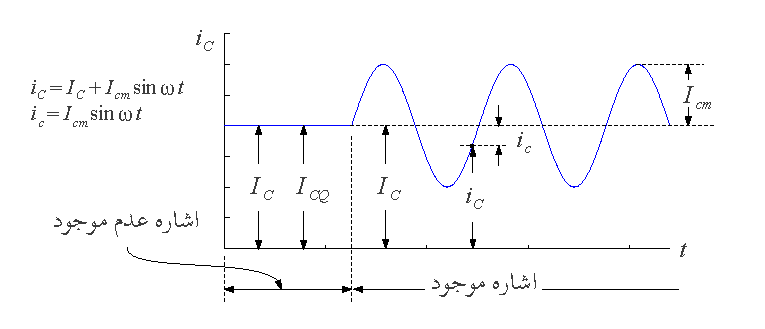
\includegraphics[scale=0.90]{definingSinusoidalWaveParameters}
\caption{سائن نما اشارہ}
\label{شکل_سائن_نما_اشارے_کے_جزو}
\end{figure}

\begin{figure}
\centering
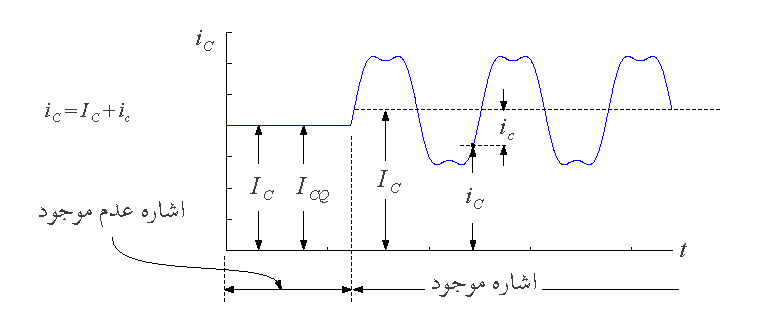
\includegraphics[scale=0.90]{definingNonSinusoidalWaveParameters}
\caption{غیر سائن نما اشارہ}
\label{شکل_غیر_سائن_نما_اشارے_کے_جزو}
\end{figure}

\FloatBarrier



\begin{tabular}{r l}
\hline
\multicolumn{2}{c}{اصطلاحات} \\
\hline
برقی دباو & \تحریر{voltage}\\
برقی رو & \تحریر{current} \\
برقی مزاحمت & \تحریر{resistance} \\
برق گیر (کپیسٹر) & \تحریر{capacitor} \\
امالہ گیر & \تحریر{inductor} \\
برقی رکاوٹ & \تحریر{impedance} \\
منبع برقی دباو & \تحریر{voltage source}\\
منبع برقی رو & \تحریر{current source} \\
تابع منبع برقی دباو & \تحریر{dependent voltage source} \\
غیر تابع منبع برقی دباو & \تحریر{independent voltage source} \\
حسابی ایمپلیفائر & \تحریر{OPAMP}\\
تفرقی جوڑا & \تحریر{difference pair} \\
اشارہ & \تحریر{signal} \\
منبع اشارہ & \تحریر{signal generator}\\
تعدد & \تحریر{frequency} \\
دو جوڑ ٹرانزسٹر & \تحریر{BJT transistor}\\
ڈایوڈ  & \تحریر{diode}\\
ماسفیٹ & \تحریر{mosfet}\\
حیطہ سوار اشارہ & \تحریر{AM signal}
\end{tabular}


\mainmatter                      %added this
%%\pagenumbering{arabic}   %instead of this

\pagestyle{headings}


\باب{حسابی ایمپلیفائر}

\اصطلاح{ٹرانزسٹر}\حاشیہب{transistor}  کی ایجاد سے اب تک الیکٹرانکس کے میدان میں ناقابل یقین اور حیرت انگیز ترقی ہوئی ہے۔شروع میں الگ الگ ٹرانزسٹر استعمال کر کے الیکٹرانک ادوار بنائے جاتے تھے۔بعد میں سلیکان کی پتری\حاشیہب{silicon chip}  پر ایک سے زیادہ ٹرانزسٹر بنانے کا رجحان پیدا ہوا۔اس طرح \اصطلاح{مخلوط ادوار}\فرہنگ{مخلوط ادوار}\حاشیہب{integrated chip (IC)}  وجود میں آئے۔ایک مربع سنٹی میٹر رقبہ کی سلیکان پتری\حاشیہد{ہائیڈروجن اور آکسیجن کے ملاپ سے پانی \عددی{\ce{H2O}} بنتا ہے۔اسی طرح سلیکان اور آکسیجن کے ملاپ سے \عددی{\ce{SiO2}} یعنی ریت یا مٹی بنتی ہے} پر اربوں ٹرانزسٹر بنانا ممکن ہوا اور دیکھتے ہی دیکھتے الیکٹرانک اشیاء  زندگی کے ہر شعبے پر چھا گئیں۔

اس کتاب میں الیکٹرانک پرزہ جات کی کارکردگی اور ان کے استعمال سے الیکٹرانک ادوار بنانے پر غور کیا جائے گا۔پہلے باب میں \اصطلاح{حسابی ایمپلیفائر}\فرہنگ{حسابی ایمپلیفائر}\حاشیہب{operational amplifier (OPAMP)}  پر غور کیا جائے گا۔حسابی ایمپلیفائر در حقیقت کئی ٹرانزسٹر پر مبنی ایک نہایت مقبول مخلوط دور ہے جس کا استعمال، برقی پرزہ جات مثلاً مزاحمت، کپیسٹر وغیرہ  کی طرح، نہایت آسان ہے۔حسابی ایمپلیفائر کی اندرونی ساخت پر اس کتاب میں آگے جا کر ایک مکمل باب ہے۔

\حصہ{حسابی ایمپلیفائر کے سرے یا پنیے}
	
حسابی ایمپلیفائر کی علامت شکل \حوالہ{شکل_حسابی_ایمپلیفائر_کی_علامت} الف  میں دکھائی گئی ہے۔حسابی ایمپلیفائر کے عموماً تین سرے ہوتے ہیں جن میں سے دو اس کے داخلی اور ایک خارجی سرا ہوتا ہے۔یوں شکل-الف میں ایک نمبر پنیا\حاشیہد{پنیوں کو نمبر کرنے کا طریقہ جلد بتلایا جائے گا} اس کا خارجی سرا ہے جبکہ دو اور تین نمبر پنیے اس کے داخلی سرے ہیں۔شکل  ب     میں حسابی ایمپلیفائر کی علامت میں دو مزید طاقت کے سرے بھی دکھائے گئے ہیں جو حسابی ایمپلیفائر کو برقی طاقت مہیا کرنے کی خاطر استعمال ہوتے ہیں۔حسابی ایمپلیفائر اُسی وقت کام کر سکتا ہے جب ان طاقت کے پنیوں پر درکار برقی طاقت مہیا کی جائے۔شکل \حوالہ{شکل_حسابی_ایمپلیفائر_کی_علامت} ب میں چار نمبر سرا مثبت برقی طاقت کا سرا ہے لہٰذا اس  پر مثبت برقی دباو مہیا کی گئی ہے  جبکہ گیارہ نمبر سرا منفی طاقت کا سرا ہے لہٰذا اس  پر منفی برقی دباو مہیا کی گئی ہے۔حسابی ایمپلیفائر ان مہیا کردہ برقی دباو سے برقی طاقت حاصل کرتا ہے۔روایتی طور پر مثبت برقی دباو کو \عددی{V_{CC}} اور منفی برقی دباو  کو \عددی{V_{EE}} پکارا جاتا ہے۔یوں شکل میں \عددی{V_{CC}=\SI{+12}{\volt}}اور \عددی{V_{EE}=\SI{-12}{\volt}}ہیں۔
\begin{figure}
\centering
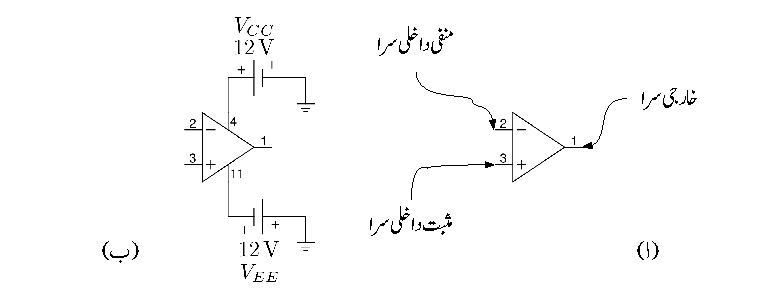
\includegraphics[scale=0.90]{opampSymbol}
\caption{حسابی ایمپلیفائر کی علامت}
\label{شکل_حسابی_ایمپلیفائر_کی_علامت}
\end{figure}
حسابی ایمپلیفائر کو عموماً شکل \حوالہ{شکل_حسابی_ایمپلیفائر_کی_علامت} الف کی علامت سے ظاہر کرتے ہوئے طاقت پنیوں کو نہیں دکھایا جاتا۔

مثبت برقی دباو اور منفی برقی دباو عموماً \اصطلاح{منبع برقی دباو} سے مہیا کیا جاتا ہے۔اس کتاب میں اس آلہ کو \اصطلاح{منبع برقی دباو}،  \اصطلاح{برقی دباو کی منبع}\حاشیہب{voltage source} یا \اصطلاح{طاقت کی منبع}\فرہنگ{طاقت کی منبع}\حاشیہب{power supply}  پکارا جائے گا۔

صنعت کار ایک یا ایک سے زیادہ تعداد میں حسابی ایمپلیفائر پلاسٹک کی ڈبیا میں بند کرتے ہیں۔شکل \حوالہ{شکل_حسابی_ایمپلیفائر_کی_ڈبیا} میں ایک ہی ڈبیا میں چار حسابی ایمپلیفائر دکھائے گئے ہیں۔ڈبیا میں بند تمام حسابی ایمپلیفائر کے \عددیء{V_{CC}} آپس میں جوڑ کر چار نمبر پنیا پر جبکہ  تمام \عددیء{V_{EE}}  کو آپس میں جوڑ کر گیارہ نمبر پنیا پر پہنچایا گیا ہے۔ڈبیا پر باریک کٹ لگایا جاتا ہے۔اس کٹ سے گھڑی کی الٹ سمت گھومتے ہوئے پنیوں کو نمبر کیا جاتا ہے۔شکل \حوالہ{شکل_حسابی_ایمپلیفائر_کی_علامت} میں حسابی ایمپلیفائر کے پنیوں پر  لکھے گئے نمبر ڈبیا کے پنیوں کو ظاہر کرتے ہیں۔ 
\begin{figure}
\centering
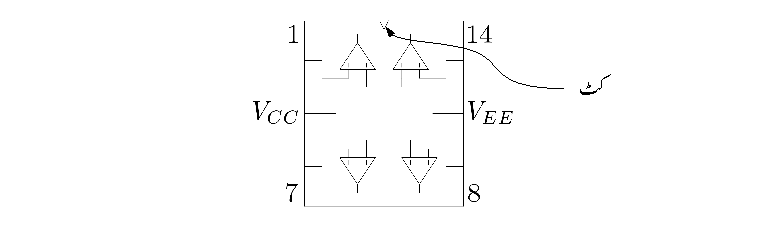
\includegraphics[scale=0.90]{opampLayout}
\caption{حسابی ایمپلیفائر کی ڈبیا}
\label{شکل_حسابی_ایمپلیفائر_کی_ڈبیا}
\end{figure}
\حصہ{حسابی ایمپلیفائر کی بنیادی کارکردگی}

حسابی ایمپلیفائر کی بنیادی کارکردگی کچھ یوں ہے۔اگر حسابی ایمپلیفائر کے دو داخلی سروں کے مابین \اصطلاح{تفرقی برقی اشارہ}\فرہنگ{تفرقی!برقی اشارہ} \عددی{v_d}\حاشیہب{differential voltage signal} مہیا کیا جائے تو یہ خارجی سرے پر\عددی{v_d} کو \عددی{A_d} گنا بڑھا کر خارج کرے گا، یعنی خارجی اشارہ \عددی{v_o}اور داخلی اشارہ \عددی{v_d}کا تعلق مندرجہ ذیل ہے
\begin{align} 
\label{مساوات_حسابی_بنیادی_کارکردگی}
v_o=A_d \times v_d
\end{align}
جہاں
\begin{align}
v_d=v_2-v_1
\end{align}
کے برابر ہے۔شکل \حوالہ{شکل_حسابی_ایمپلیفائر_کی_کارکردگی}  میں اس حقیقت کو دکھایا گیا ہے۔\عددی{A_d} کو ایمپلیفائر کا \اصطلاح{تفرقی برقی دباو کی افزائش}\فرہنگ{تفرقی!افزائش برقی دباو}\فرہنگ{differential voltage gain}\حاشیہب{differential voltage gain} یا \اصطلاح{برقی دباو کی تفرقی افزائش} کہتے ہیں۔یوں حسابی ایمپلیفائر کو \اصطلاح{تفرقی ایمپلیفائر}\فرہنگ{تفرقی!ایمپلیفائر}\حاشیہب{difference amplifier}\فرہنگ{amplifier!difference} بھی کہتے ہیں۔مساوات \حوالہ{مساوات_حسابی_بنیادی_کارکردگی}  میں اگر داخلی اشارہ کو دگنا کر دیا جائے تو خارجی اشارہ بھی دگنا ہو جائے گا۔یوں حسابی ایمپلیفائر کی کارکردگی \اصطلاح{خطی}\فرہنگ{خطی}\حاشیہب{linear relation} نوعیت کی ہے۔
	
یہاں اس بات کا ذکر کرنا ضروری ہے کہ حسابی ایمپلیفائر کے خارجی اشارہ \عددی{v_o}کی قیمت کسی صورت مثبت برقی دباو \عددی {V_{CC}} سے زیادہ یا منفی برقی دباو \عددی{V_{EE}} سے کم نہیں ہو سکتی۔ حقیقت میں \عددی{v_o} کی زیادہ سے زیادہ ممکنہ حد \عددی{V_{CC}}سے،\عددی{1} تا\عددی{3} وولٹ کم ہوتا ہے۔اسی طرح \عددی{v_o}کی کم سے کم ممکنہ حد  \عددی {V_{EE}}  سے، \عددی{1}  تا \عددی{3} وولٹ زیادہ ہوتا ہے۔یعنی
\begin{align}
\label{مساوات_حسابی_کے_خارجی_حدود}
(V_{EE} +\Delta_{-} )  <  v_o  < (V_{CC} -\Delta_{+})
\end{align}
اس مساوات میں \عددی{\Delta_{+}} اور \عددی{\Delta_{-}} ایک سے تین وولٹ کو ظاہر کرتے ہیں۔اس کتاب میں جب تک کہا نہ جائے ہم  \عددی{\Delta_{+}} اور  \عددی{\Delta_{-}} کی قیمت صفر تصور کریں گے۔یوں \عددی{v_o} مثبت برقی دباو \عددی{V_{CC}} سے لے کر منفی برقی دباو \عددی{V_{EE}}تک کی قیمت اختیار کر سکتا ہے۔حصہ \حوالہ{جزو_حسابی_ایمپلیفائر_کا_لبریز_ہونا} میں اس عمل پر تذکرہ کیا جائے گا۔



اگر حسابی ایمپلیفائر کو مہیا \اصطلاح{تفرقی اشارہ} \عددی{v_d}کی قیمت اتنی ہو کہ مساوات \حوالہ{مساوات_حسابی_بنیادی_کارکردگی}   سے حاصل \عددی{v_o} کی قیمت مساوات \حوالہ{مساوات_حسابی_کے_خارجی_حدود}  میں دیے حدود سے تجاوز کرے تو اس صورت میں حسابی ایمپلیفائر مساوات \حوالہ{مساوات_حسابی_بنیادی_کارکردگی}  پر پورا نہیں اترے گا جبکہ اس کی  \عددی{v_o}   مساوات \حوالہ{مساوات_حسابی_کے_خارجی_حدود}  میں دیے حدود کے اندر ہی رہے گی۔اس صورت میں مثبت جانب بڑھتے ہوئے\عددی{v_o}  کی قیمت \عددی{(V_{CC}-\Delta_{+})} تک پہنچ کر رک جائے گی یا پھر منفی جانب گھٹتے ہوئے \عددی{v_o} کی قیمت  \عددی{(V_{CC}-\Delta_{-})} تک پہنچ کر رک جائے گی۔اس صورت میں  \عددی{\abs{v_d}} کو مزید بڑھانے سے \عددی{v_o} کی قیمت پر کوئی اثر نہیں ہوتا۔اس صورت میں حسابی ایمپلیفائر کی کارکردگی غیر خطی ہو گی اور اس کو حسابی ایمپلیفائر کا \اصطلاح{لبریز}\فرہنگ{لبریز}
\فرہنگ{saturation!OPAMP}\حاشیہب{saturation}  ہونا کہتے ہیں۔
\begin{figure}
\centering
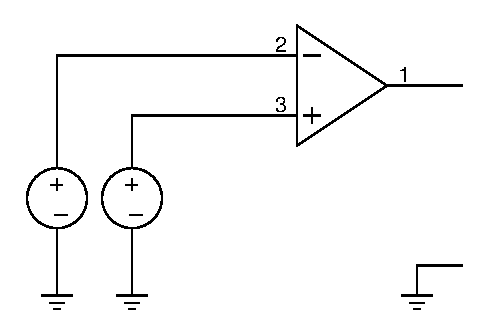
\includegraphics[scale=0.90]{opampWorking}
\caption{حسابی ایمپلیفائر کی کارکردگی}
\label{شکل_حسابی_ایمپلیفائر_کی_کارکردگی}
\end{figure}
%==============================
\ابتدا{مثال}
ایک حسابی ایمپلیفائر جس کی \اصطلاح{تفرقی افزائش برقی دباو} \عددی{A_d}  کی قیمت \عددی{\SI{100000}{\volt \per \volt}} ہے کو اس کے داخلی سروں پر مندرجہ ذیل برقی دباو مہیا کئے جاتے ہیں۔
\begin{enumerate}
\item
\عددی{v_1=\SI{0}{\volt}} اور \عددی{v_2 = \SI{10}{\micro \volt}}
\item
\عددی{v_1=\SI{10}{\micro \volt}} اور \عددی{v_2 = \SI{0}{\volt}}
\item
\عددی{v_1=\SI{2.00003}{\volt}} اور \عددی{v_2 = \SI{2.00005}{\volt}}
\item
\عددی{v_1=\SI{2.0003}{\volt}} اور \عددی{v_2 = \SI{2.0005}{\volt}}
\item
\عددی{v_1=\SI{2.05}{\volt}} اور \عددی{v_2 = \SI{2.03}{\volt}}

\item
\عددی{v_1=\SI{2.03}{\volt}} اور \عددی{v_2 =\SI{2.03}{\volt}}
\end{enumerate}
\عددی{V_{CC}=\SI{+12}{\volt}}اور \عددی{V_{EE}=\SI{-12}{\volt}} جبکہ \عددی{\Delta_+ = \Delta_- = 0} ہونے کی صورت میں حسابی ایمپلیفائر کی \عددی{v_o} دریافت کریں۔


حل:	جب تک \عددی{v_o} مساوات \حوالہ{مساوات_حسابی_کے_خارجی_حدود}  میں دیے حدود کے اندر رہے، حسابی ایمپلیفائر داخلی برقی دباو کو ایک لاکھ مرتبہ بڑھا کر خارج کرے گا۔یوں
\begin{enumerate}
\item $\begin{aligned}[t]
v_0 &=A_d \times v_d \\
&=A_d \times \left (v_2 - v_1 \right )\\
&=100000 \times \left(10\times 10^{-6}-0 \right )\\
&=\SI{1}{\volt}
\end{aligned}$
%
\item $\begin{aligned}[t]
v_0 &=A_d \times v_d \\
&=A_d \times \left (v_2 - v_1 \right )\\
&=100000 \times \left(0-10\times 10^{-6} \right )\\
&=\SI{-1}{\volt}
\end{aligned}$
%
\item $\begin{aligned}[t]
v_0 &=A_d \times v_d \\
&=A_d \times \left (v_2 - v_1 \right )\\
&=100000 \times \left(2.00005-2.00003 \right )\\
&=\SI{2}{\volt}
\end{aligned}$

\item $\begin{aligned}[t]
v_0 &=A_d \times v_d \\
&=A_d \times \left (v_2 - v_1 \right )\\
&=100000 \times \left(2.0005-2.0003 \right )\\
&=\SI{20}{\volt}
\end{aligned}$

چوتھے صورت میں \عددی{v_o} کی قیمت مساوات \حوالہ{مساوات_حسابی_کے_خارجی_حدود} میں دیے حدود سے تجاوز کر گئی جو کہ ناممکن صورتِ حال ہے۔لہٰذا اس جواب کو رد کیا جاتا ہے۔اس صورت میں حسابی ایمپلیفائر کی کوشش ہو گی کہ \عددی{v_o} کی قیمت بیس وولٹ ہو لیکن حسابی ایمپلیفائر ایسا کرنے سے عاجز ہے  کیونکہ اس کے خارجی اشارے  کی قیمت \عددی{V_{CC}} کی قیمت سے زیادہ نہیں ہو سکتی۔لہٰذا  \عددی{ \Delta_+ = \Delta_- = 0} لیتے ہوئے اس صورت میں  \عددی{v_o}زیادہ سے زیادہ ممکنہ برقی دباو کے برابر ہو گا یعنی \عددی{v_o = +12 V}ہو گا۔حقیقت میں  \عددی{v_o}کی زیادہ سے زیادہ ممکنہ قیمت\عددی{V_{CC}}  سے ایک یا دو وولٹ کم ہوتی ہے۔حسابی ایمپلیفائر بنانے والے یہ معلومات فراہم کرتے ہیں۔
\item $\begin{aligned}[t]
v_0 &=A_d \times v_d \\
&=A_d \times \left (v_2 - v_1 \right )\\
&=100000 \times \left(2.03-2.05 \right )\\
&=\SI{-2000}{\volt}
\end{aligned}$

یہاں \عددی{v_o} کی قیمت مساوات \حوالہ{مساوات_حسابی_کے_خارجی_حدود}  میں دیے حدود سے تجاوز کر گئی جو کہ ناممکن صورتِ حال ہے۔اس صورت میں  \عددی{v_o}کی قیمت  \عددی{V_{EE}} سے قدر زیادہ قیمت اختیار کرے گی۔ \عددی{\Delta_+ = \Delta_- = 0}لیتے ہوئے اس صورت\عددی{v_o=\SI{-12}{\volt}} ہو گی۔
\item $\begin{aligned}[t]
v_0 &=A_d \times v_d \\
&=A_d \times \left (v_2 - v_1 \right )\\
&=100000 \times \left(2.03-2.03 \right )\\
&=\SI{0}{\volt}
\end{aligned}$
\end{enumerate}
یہاں آپ نے دیکھا کہ دونوں داخلی سروں پر برابر برقی دباو مہیا کرنے سے حسابی ایمپلیفائر صفر وولٹ خارج کرتا ہے۔ دونوں داخلی سروں پر برابر مہیا کردہ برقی دباو کو \اصطلاح{مشترکہ برقی دباو}\فرہنگ{مشترکہ برقی دباو}\فرہنگ{common mode voltage}\حاشیہب{common mode voltage}  کہتے ہیں۔ حسابی ایمپلیفائر مشترکہ برقی دباو کو رد کرتا ہے۔


یہاں یہ بتلاتا چلوں کہ کسی بھی داخلی برقی دباو کو \اصطلاح{مشترکہ برقی دباو} \عددی{v_{CM}} اور \اصطلاح{تفرقی برقی دباو}\فرہنگ{تفرقی!برقی دباو}\فرہنگ{differential mode voltage}\حاشیہب{differential mode voltage} \عددی{v_d} میں تقسیم کیا جا سکتا ہے۔پانچویں جزو میں \عددی{v_1 = \SI{2.05}{\volt}} اور \عددی{v_2 = \SI{2.03}{\volt}} کو یوں بیان کیا جا سکتا ہے کہ حسابی ایمپلیفائر کو 
\( \tfrac{2.05+2.03}{2}=\SI{2.04}{\volt} \)
بطور مشترکہ برقی دباو فراہم کئے گئے جبکہ اسے
\( 2.03-2.05=\SI{-0.02}{\volt}\)
بطور تفرقی برقی دباو مہیا کئے گئے۔

\انتہا{مثال}
%=====================

	اس مثال میں آپ نے دیکھا کہ چند مائیکرو وولٹ\حاشیہب{\si{\micro \volt}} برقی دباو کو حسابی ایمپلیفائر بڑھا کر وولٹ کی حد میں لے آتا ہے۔یہاں آپ کی دلچسپی کی خاطر بتلاتا چلوں کہ انسانی اعصابی نظام  ستر ملی وولٹ \عددی{\SI{70}{\milli \volt}} کے لگ بھگ برقی دباو پر کام کرتا ہے۔یوں حسابی ایمپلیفائر استعمال کرتے ہوئے  آپ اعصابی نظام کے کارکردگی پر تحقیق کر سکتے ہیں۔ 

	اس مثال کے پہلے دو حصوں میں آپ نے دیکھا کہ اگر داخلی برقی دباو کو حسابی ایمپلیفائر کے \اصطلاح{مثبت داخلی سرے}\فرہنگ{مثبت داخلی سرا}\حاشیہب{non-inverting input}  پر مہیا کیا جائے تو اس سے حاصل خارجی برقی دباو کی علامت تبدیل نہیں ہوتی۔یعنی اگر مثبت برقی دباو مہیا کی جائے تو مثبت برقی دباو ہی خارج کی جاتی ہے۔اس کے برعکس اگر برقی دباو کو حسابی ایمپلیفائر کے \اصطلاح{منفی داخلی سرے}\فرہنگ{منفی داخلی سرا}\حاشیہب{inverting input}  پر مہیا کیا جائے تو اس سے حاصل خارجی برقی دباو کی علامت تبدیل ہو جاتی ہے۔یعنی اگر مثبت برقی دباو مہیا کی جائے تو منفی برقی دباو خارج کی جاتی ہے۔

\حصہ{ حسابی ایمپلیفائر کا مساوی دور یا ریاضی نمونہ}
حسابی ایمپلیفائر کا مساوی دور شکل \حوالہ{شکل_حسابی_ایمپلیفائر_کا_مساوی_دور} میں دکھایا\حاشیہد{اس شکل میں تفرقی برقی دباو کا مثبت سرا نچلی جانب ہے۔} گیا ہے۔
\begin{figure}
\centering

\includegraphics[scale=0.90]{opampEquivalentCircuit}
\caption{حسابی ایمپلیفائر کا مساوی دور (ریاضی نمونہ)}
\label{شکل_حسابی_ایمپلیفائر_کا_مساوی_دور}
\end{figure}
جیسا کہ شکل سے واضح ہے داخلی جانب سے حسابی ایمپلیفائر بالکل ایک مزاحمت \عددی{R_i} کی طرح معلوم ہوتا ہے جبکہ خارجی جانب  یہ  \اصطلاح{تابع منبع دباو}\فرہنگ{تابع منبع دباو}\حاشیہب{depended voltage source}\فرہنگ{depended voltage source}جس کے ساتھ سلسلہ وار مزاحمت \عددی{R_o} جڑی ہو معلوم ہوتا ہے۔تابع منبع دباو،  داخلی جانب مہیا اشارہ \عددی{v_d} کے تابع ہے۔

	حسابی ایمپلیفائر کے صنعت کاروں کی کوشش ہوتی ہے کہ حسابی ایمپلیفائر کے \اصطلاح{داخلی مزاحمت}\فرہنگ{داخلی مزاحمت} \عددی{R_i} کی قیمت زیادہ سے زیادہ جبکہ  \اصطلاح{خارجی مزاحمت}\فرہنگ{خارجی مزاحمت} \عددی{R_o} کی قیمت کم سے کم ہو۔اسی طرح کوشش کی جاتی ہے کہ \اصطلاح{تفرقی افزائش برقی دباو}\فرہنگ{تفرقی!افزائش برقی دباو}  \عددی{A_d} کی قیمت زیادہ سے زیادہ ہو۔جدول \حوالہ{جدول_حسابی_ایمپلیفائر_عمومی_مقداریں} میں آپ کے اندازے کی خاطر ایک عام دستیاب حسابی ایمپلیفائر\حاشیہد{عام دستیاب ایمپلیفائر کی قیمت بازار میں فروخت ہونے والی  تندور کی دو روٹیوں کے لگ بھگ ہے} کے  \اصطلاح{ریاضی نمونے}\فرہنگ{ریاضی نمونہ}\فرہنگ{نمونہ!ریاضی}\حاشیہب{model}\فرہنگ{model} کے اجزاء دئے گئے ہیں۔
\begin{table}[ht]
\caption{عام دستیاب حسابی ایمپلیفائر کے ریاضی نمونے کی مقررہ مقداریں}
\label{جدول_حسابی_ایمپلیفائر_عمومی_مقداریں}
\centering
\begin{tabular}{l l}
\toprule
$R_i$ &  $\SI{e{12}}{\ohm}$ \\
$R_o$ & $\SI{100}{\ohm}$\\
$A_d$  & $\SI[per=frac,fraction=nice]{100000}{\volt \per \volt}$ \\
\bottomrule
\end{tabular}
\end{table}
ان مقداروں کو مثال بناتے ہوئے شکل \حوالہ{شکل_حسابی_ایمپلیفائر_کا_مساوی_دور} پر غور کرتے ہیں۔

\جزوحصہ{داخلی سروں پر برابر برقی دباو رہتا ہے}

حسابی ایمپلیفائر کو عام طور  پر خطی کارکردگی کے احاطے میں استعمال کیا جاتا ہے یعنی اسے  استعمال کرتے ہوئے  \عددی{v_d} کی قیمت اتنی رکھی جاتی ہے کہ \عددی{v_o} مساوات \حوالہ{مساوات_حسابی_کے_خارجی_حدود} میں دیے حدود کے اندر رہے۔\عددی{V_{CC}=\SI{+12}{\volt}} اور \عددی{V_{EE}=\SI{-12}{\volt}} لیتے ہوئے \عددی{v_o} کی زیادہ سے زیادہ ممکنہ قیمت تقریباً \عددی{\SI{+12}{\volt}}اور کم سے کم ممکنہ قیمت تقریباً \عددی{\SI{-12}{\volt}} ہے۔جب \عددی{v_o = \SI{+12}{\volt}}ہو،  اس وقت مساوات \حوالہ{مساوات_حسابی_بنیادی_کارکردگی}  کے تحت \عددی{v_d =\SI{120}{\micro \volt}} ہو گا اور جب  \عددی{v_o = \SI{-12}{\volt}} ہو اس وقت\عددی{v_d =\SI{-120}{\micro \volt}} ہو گا۔یوں حسابی ایمپلیفائر کو خطی خطے میں استعمال کرتے ہوئے \عددی{\abs{v_d} < \SI{120}{\micro \volt}} رہے گا۔شکل \حوالہ{شکل_حسابی_ایمپلیفائر_کی_کارکردگی}  کو دیکھتے ہوئے اس بات کو یوں بیان کر سکتے ہیں کہ
\begin{align}
\abs{v_d} =\abs{v_2-v_1} < \SI{120}{\micro \volt}
\end{align}
رکھتے ہوئے حسابی ایمپلیفائر خطی خطے میں رہتا ہے۔\عددی{\SI{120}{\micro \volt}} اتنی کم برقی دباو ہے کہ اسے نظر انداز کیا جا سکتا ہے۔ایسا کرنے سے حسابی ایمپلیفائر پر مبنی ادوار کو حل کرنا نہایت آسان ہو جاتا ہے۔یوں  اس مساوات کو اس طرح لکھا جا سکتا ہے
\begin{gather}
\begin{aligned} \label{مساوات_حسابی_داخلی_سروں_پر_برابر_دباو}
\abs{v_2  -  v_1} &\approx 0   \\
v_2 & \approx v_1
\end{aligned}
\end{gather}
	یہ نہایت اہم مساوات ہے  جسے  بار بار استعمال کیا جائے گا۔اس مساوات کے تحت جب تک حسابی ایمپلیفائر کو خطی احاطے میں استعمال کیا جائے اس وقت تک اس کے دونوں داخلی سروں پر تقریباً برابر برقی دباو ہو گا۔

	اوپر مثال کو دوبارہ دیکھتے ہوئے پہلی دو صورتوں میں \عددی{v_2 \approx v_1 \approx 0}ہے جبکہ تیسری صورت میں \عددی{v_2 \approx v_1 \approx \SI{2}{\volt}} ہے۔ان میں حسابی ایمپلیفائر خطی احاطے میں کام کر رہا ہے۔چوتھی اور پانچویں صورتوں میں یہ غیر خطی احاطے میں کام کر رہا ہے۔پانچویں صورت میں یہ بات زیادہ واضح سامنے آتی ہے کہ \عددی{v_2} اور\عددی{v_1} برابر نہیں۔یہاں ان میں  \عددی{\SI{20}{\milli \volt}} کا فرق ہے جسے نظر انداز نہیں کیا جا سکتا۔

\جزوحصہ{داخلی سروں پر برقی رو صفر ہوتی ہے}
	آپ نے دیکھا کہ حسابی ایمپلیفائر کو خطی احاطے میں استعمال کرتے ہوئے  \عددی{\abs{v_d}< \SI{120}{\micro \volt}} رہتا ہے۔اگر \عددی{R_i=\SI{e12}{\ohm}}ہو تو شکل \حوالہ{شکل_حسابی_ایمپلیفائر_کا_مساوی_دور}  کو دیکھتے ہوئے مزاحمت \عددی{R_i}میں برقی رو \عددی{i} کی قیمت
\begin{align}
i=\frac{v_d}{R_i} =\frac{\abs{120 \times 10^{-6}}}{10^{12}}=\SI{1.2e-16}{\ampere}
\end{align}
ہو گی جو کہ قابل نظر انداز قیمت ہے۔یوں ہم کہہ سکتے ہیں کہ حسابی ایمپلیفائر کے داخلی سروں پر برقی رو کی قیمت صفر ایمپیئر ہو گی یا یہ کہ ان سروں کو مکمل طور منقطع تصور کیا جا سکتا ہے۔یوں
\begin{align} \label{مساوات_حسابی_صفر_داخلی_رو}
{i \approx \SI{0}{\ampere}}
\end{align}
تصور کیا جاتا ہے۔

\جزوحصہ{داخلی مزاحمت کو لامحدود تصور کیا جاتا ہے}

	جیسا کہ جدول  میں ذکر ہوا حسابی ایمپلیفائر کے داخلی مزاحمت \عددی{R_i}کی قیمت نہایت بڑی ہوتی ہے۔اتنی مزاحمت کو یقیناً لامحدود تصور کیا جا سکتا ہے یعنی
\begin{align} \label{مساوات_حسابی_لامحدود_داخلی_مزاحمت}
R_i \to \infty
\end{align}
اس کا مطلب ہے کہ داخلی سروں کو آپس میں مکمل طور منقطع سمجھا جا سکتا ہے۔


\جزوحصہ{تفرقی افزائش کو لامحدود تصور کیا جاتا ہے}

جدول \حوالہ{جدول_حسابی_ایمپلیفائر_عمومی_مقداریں} میں تفرقی افزائش برقی دباو کی مثال \عددی{A_d =\SI[per=frac,fraction=nice]{100000}{\volt \per \volt}} دی گئی ہے جسے لامحدود تصور کیا جا سکتا ہے یعنی
\begin{align}
A_D \to \infty
\end{align}
اس مساوات کو دیکھتے یہ خیال آتا ہے کہ لامحدود افزائش کی صورت میں اسے استعمال کیسے کیا جائے گا۔درحقیقت حسابی ایمپلیفائر کو عموماً واپسی اشارہ\حاشیہب{feedback signal}  مہیا کرتے ہوئے استعمال کیا جاتا۔اس بات کی وضاحت حصہ \حوالہ{حصہ_حسابی_ایمپلیفائر_کے_ادوار} میں ہو جائے گی۔


\جزوحصہ{خارجی مزاحمت کو صفر اُوہم تصور کیا جا سکتا ہے}
	
آپ دیکھیں گے کہ عام استعمال میں حسابی ایمپلیفائر کے خارجی جانب جڑے بیرونی مزاحمتوں کی قیمتیں کلو اُوہم  \عددیء{\SI{}{\kilo \ohm}} کے حدود میں ہو گی جو کہ  \عددی{R_o} کی قیمت سے کئی گنا زیادہ ہے۔یوں حسابی ایمپلیفائر پر مبنی ادوار حل کرتے وقت اگر\عددی{R_o} کو بالکل نظر انداز کر دیا جائے تو حاصل جواب پر خاص فرق نہیں پڑے گا۔عام استعمال میں ایسا ہی تصور کیا جاتا ہے یعنی
\begin{align} \label{مساوات_حسابی_صفر_خارجی_مزاحمت}
R_o \approx \SI{0}{\ohm}
\end{align}


\حصہ{کامل حسابی ایمپلیفائر}

خطی خطے  میں استعمال ہوتے ہوئے حسابی ایمپلیفائر  کی کارکردگی پر غور کرتے ہوئے کچھ حقائق سامنے آئے جنہیں مساوات \حوالہ{مساوات_حسابی_داخلی_سروں_پر_برابر_دباو}، \حوالہ{مساوات_حسابی_صفر_داخلی_رو} ،  \حوالہ{مساوات_حسابی_لامحدود_داخلی_مزاحمت} اور \حوالہ{مساوات_حسابی_صفر_خارجی_مزاحمت} میں بیان کیا گیا۔ان مساوات کو یہاں یکجا کر کے پیش کرتے ہیں۔
\begin{gather} 
\begin{aligned}\label{مساوات_حسابی_بنیادی_پہلو}
v_2 &=v_1 \hspace{5mm} \text{\RL{خطی خطہ}}\\
i&=0\\
R_i &=\infty\\
R_o &=0
\end{aligned}
\end{gather}
ایسا کرتے وقت \عددی{\approx} اور\عددی{\to} کے علامات کی جگہ \عددی{=}کی علامت استعمال کی گئی ہے۔ان مساوات کے پہلے جزو میں خطی خطہ لکھ کر اس بات کی یاد دہانی کرائی جاتی ہے کہ داخلی سرے صرف اس صورت برابر برقی دباو پر رہتے ہیں جب تک ایمپلیفائر خطی خطے میں رہے۔اس بات کی وضاحت مثال \حوالہ{مثال_حسابی_خطی_غیر_خطی_خطے} میں ہو گی۔ان مساوات کو مد نظر رکھتے ہوئے ہم شکل \حوالہ{شکل_حسابی_ایمپلیفائر_کا_مساوی_دور}  کو دوبارہ بناتے ہیں۔ایسا کرنے سے شکل \حوالہ{شکل_کامل_حسابی_ایمپلیفائر_کا_مساوی_دور} حاصل ہوتا ہے جو کہ \اصطلاح{کامل} حسابی ایمپلیفائر\فرہنگ{کامل حسابی ایمپلیفائر}\حاشیہب{ideal} کا مساوی دور یا \اصطلاح{ریاضی نمونہ}\فرہنگ{ریاضی نمونہ}\فرہنگ{نمونہ!ریاضی}\حاشیہب{model}\فرہنگ{model}  ہے۔
\begin{figure}
\centering
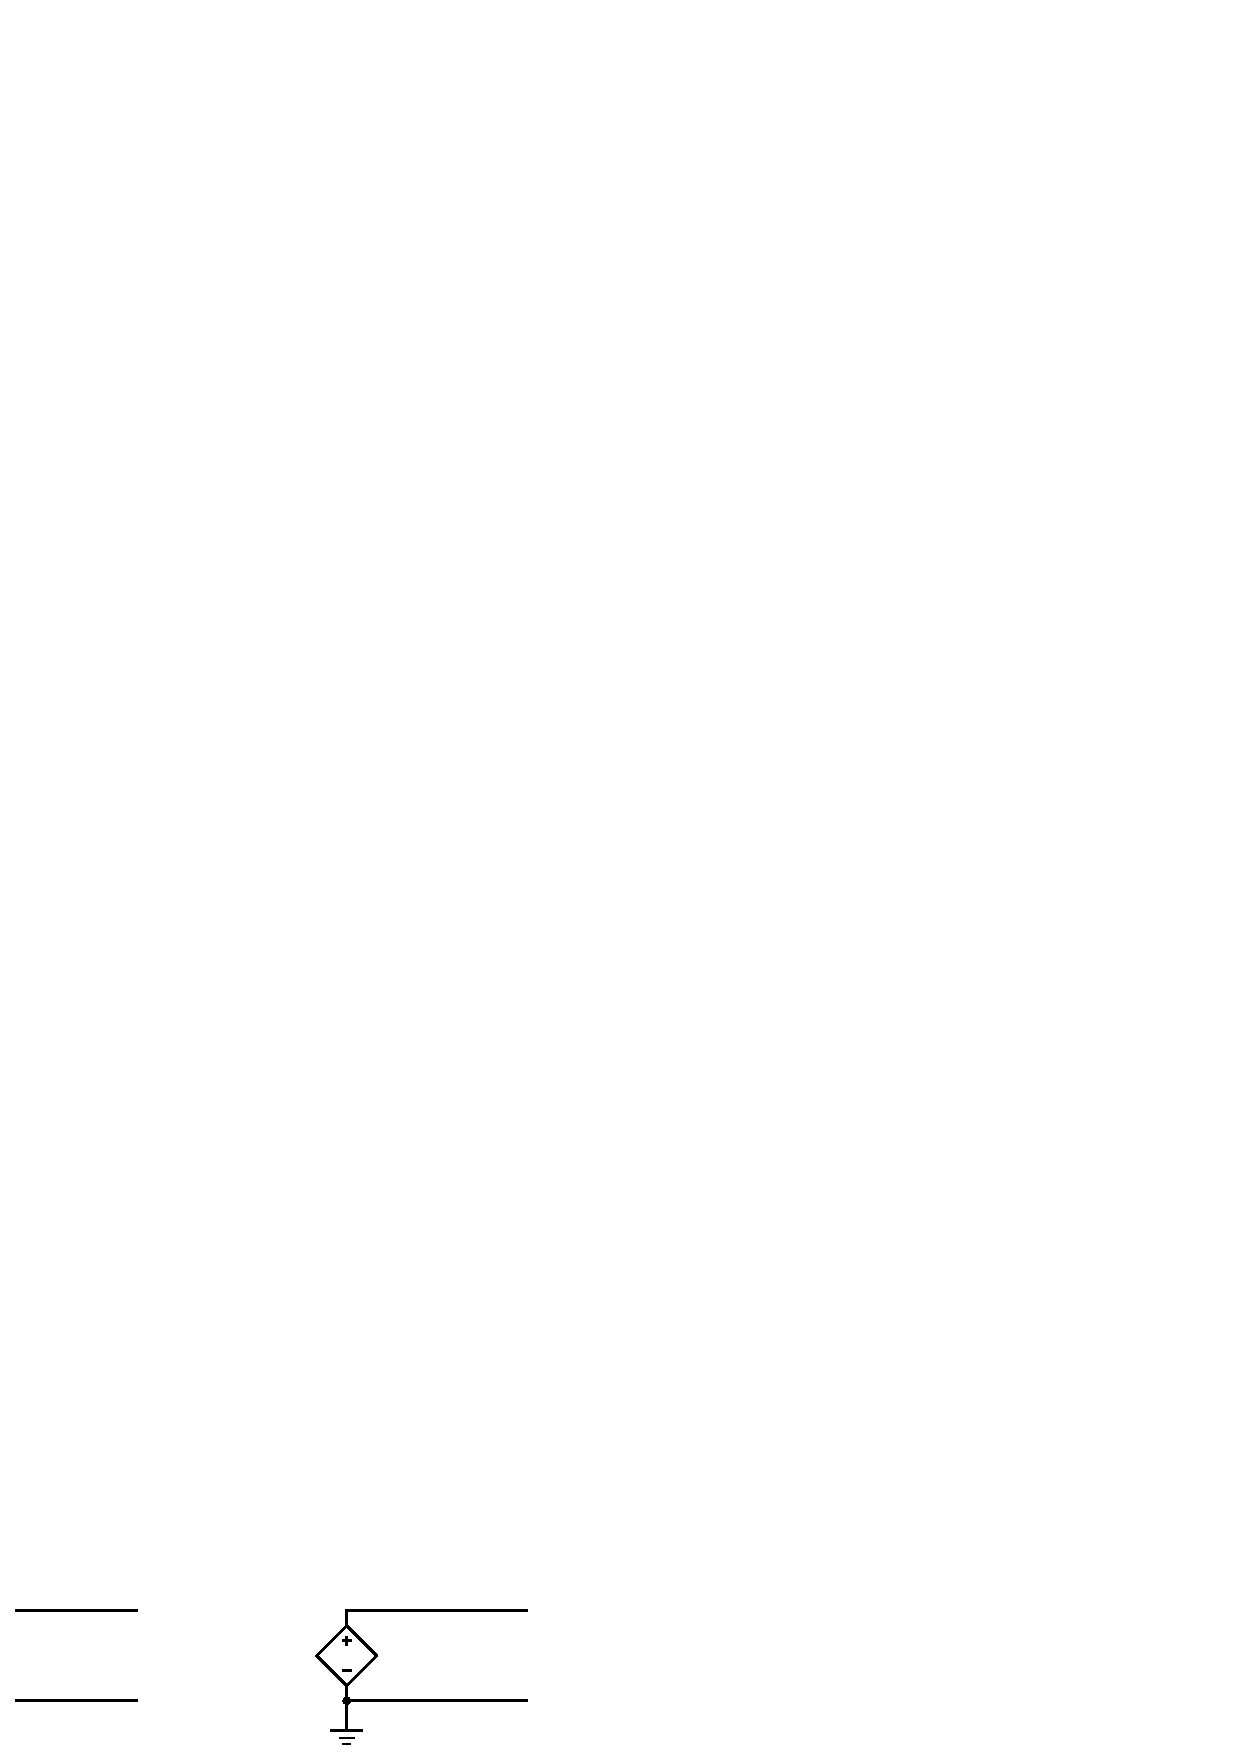
\includegraphics[scale=0.90]{idealOpampEquivalentCircuit}
\caption{کامل حسابی ایمپلیفائر کا مساوی دور یا ریاضی نمونہ}
\label{شکل_کامل_حسابی_ایمپلیفائر_کا_مساوی_دور}
\end{figure}
	اس شکل سے واضح ہے کہ داخلی سروں پر برقی رو صفر ایمپیئر ہے، داخلی مزاحمت لامحدود جبکہ خارجی مزاحمت صفر اُوہم ہے۔

\ابتدا{مثال}
\begin{itemize}
\item
جدول \حوالہ{جدول_حسابی_ایمپلیفائر_عمومی_مقداریں} میں دیے مقدار اور حسابی ایمپلیفائر کا غیر کامل مساوی دور (ریاضی نمونہ) استعمال کرتے ہوئے \عددی{v_s=\SI{1}{\volt}} پر  شکل \حوالہ{شکل_منفی_ایمپلیفائر} میں \عددی{v_o} کی قیمت حاصل کریں۔\عددی{R_1=\SI{1}{\kilo \ohm}} اور \عددی{R_2=\SI{10}{\kilo \ohm}} ہیں۔
\item
حسابی ایمپلیفائر کا کامل مساوی دور اور جدول \حوالہ{جدول_حسابی_ایمپلیفائر_عمومی_مقداریں} میں دیے گئے \عددی{A_d} کی قیمت استعمال کرتے ہوئے  دوبارہ  \عددی{v_o} کی قیمت حاصل کریں۔
\item
دونوں جوابات کا موازنہ کریں۔
\end{itemize}
%
\begin{figure}
\centering
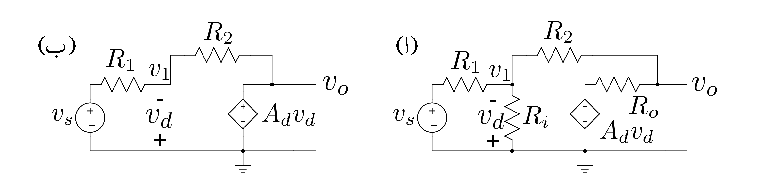
\includegraphics[scale=0.90]{opampModelUsageExample}
\caption{حسابی ایمپلیفائر کے مساوی دور (ریاضی نمونے) کا استعمال}
\label{شکل_حسابی_ماڈل_استعمال}
\end{figure}
%
حل:
شکل \حوالہ{شکل_حسابی_ماڈل_استعمال}-الف میں حسابی ایمپلیفائر کا غیر کامل مساوی دور جبکہ شکل  \حوالہ{شکل_حسابی_ماڈل_استعمال}-ب     میں اس کا کامل مساوی دور استعمال کرتے ہوئے شکل \حوالہ{شکل_منفی_ایمپلیفائر} کو بنایا گیا ہے۔
\begin{itemize}
\item
شکل-الف میں کرخوف کے قانون برائے برقی رو استعمال کرتے ہوئے
\begin{align*}
\frac{v_1-v_s}{R_1}+\frac{v_1}{R_i}+\frac{v_1-v_o}{R_2}=0\\
\frac{v_o-v_1}{R_2}+\frac{v_o-A_d v_d}{R_o}=0
\end{align*}
حاصل ہوتا ہے۔دیے گئے قیمتیں استعمال کرتے ہوئے اور \عددی{v_1=-v_d} لکھ کر حل کرتے ہیں۔
\begin{align*}
\frac{-v_d-1}{\num{1000}}+\frac{-v_d}{\num{10e12}}+\frac{-v_d-v_o}{\num{10000}}=0\\
\frac{v_o+v_d}{\num{10000}}+\frac{v_o-\num{100000} v_d}{\num{100}}=0
\end{align*}
\عددی{\tfrac{v_d}{10^{12}}} کو نظر انداز کرتے ہوئے  حاصل ہوتا ہے۔
\begin{align*}
v_d=\frac{1+0.1 v_o}{1.1}\\
v_o=\frac{\num{10000001}}{101} v_d
\end{align*}
 اور یوں
\begin{align*}
v_o=\SI{-10.00111}{\volt}
\end{align*}
حاصل ہوتا ہے۔
\item
شکل \حوالہ{شکل_حسابی_ماڈل_استعمال} ب پر کرخوف کے قانون برائے برقی رو کے استعمال کرتے ہوئے حل کرتے ہیں۔
\begin{align*}
\frac{v_1-v_s}{R_1}+\frac{v_1-A_d v_d}{R_2}=0\\
\frac{-v_d-v_s}{R_1}+\frac{-v_d-A_d v_d}{R_2}=0\\
v_d=\frac{-v_s}{1+\frac{R_1}{R_2}\left(1+A_d \right)}
\end{align*}
اور یوں \عددی{v_o=A_d v_d} لکھتے ہوئے
\begin{align} \label{مساوات_حسابی_کامل_مثال_حل}
v_o=\frac{-A_d v_s}{1+\frac{R_1}{R_2}\left(1+A_d \right)}
\end{align}
یعنی
\begin{align*}
v_o=\frac{-\num{100000} v_s}{1+\frac{\num{1000}}{\num{10000}}\left(1+\num{100000} \right)}=\SI{-9.9989}{\volt}
\end{align*}
حاصل ہوتا ہے جہاں \عددی{v_s=\SI{1}{\volt}} پُر کیا گیا ہے۔
\item
پہلے جواب کی نسبت سے دیکھتے ہوئے دونوں جوابات میں صرف
\begin{align*}
\abs{\frac{-10.00111+9.9989}{10.00111}} \times 100=\SI{0.0221}{\percent}
\end{align*}
کا فرق ہے جو کہ قابل نظر انداز ہے۔یوں اس مثال میں غیر کامل اور کامل مساوی ادوار استعمال کرتے ہوئے یکساں جوابات حاصل ہوتے ہیں۔
\end{itemize}
\انتہا{مثال}

مساوات \حوالہ{مساوات_حسابی_کامل_مثال_حل} میں \عددی{A_d \gg 1} اور  \عددی{\tfrac{R_1}{R_2} \left(1+A_d \right) \gg 1} ہے۔
یوں اس مساوات کو با آسانی اس طرح بھی حل کیا جا سکتا ہے
\begin{align*}
v_o=\frac{-A_d v_s}{1+\frac{R_1}{R_2}\left(1+A_d \right)} \approx \frac{-A_d v_s}{\frac{R_1}{R_2}\left(1+A_d \right)}  \approx \frac{-A_d v_s}{\frac{R_1}{R_2}\left(A_d \right)} =-\frac{R_2}{R_1}v_s
\end{align*}

یہی جواب \عددی{A_d \gg 1} اور  \عددی{\tfrac{R_1}{R_2} \left(1+A_d \right) \gg 1} کے  حقائق (یا شرائط) کی بجائے  \عددی{A_d \to \infty} تصور کرتے ہوئے بھی حاصل  کیا جا سکتا تھا۔

اس مثال میں حسابی ایمپلیفائر کے ساتھ بیرونی جوڑے گئے مزاحمت \عددی{R_1} اور \عددی{R_2} کی قیمتیں حسابی ایمپلیفائر کے اندرونی مزاحمت \عددی{R_i} سے بہت کم اور اندرونی مزاحمت \عددی{R_o} سے بہت زیادہ تھیں۔مزید یہ کہ \عددی{A_d} کی قیمت کو لامحدود تصور کرتے ہوئے زیادہ آسانی سے جواب حاصل ہوتا ہے۔

جب بھی حسابی ایمپلیفائر کے ساتھ بیرونی جڑے مزاحمت کی قیمت \عددی{R_i} سے بہت کم اور \عددی{R_o} سے بہت زیادہ ہو، ایسی صورت میں غیر کامل اور کامل مساوی ادوار دونوں کے استعمال سے یکساں جوابات حاصل ہوتے ہیں۔چونکہ کامل دور استعمال کرتے ہوئے جواب زیادہ آسانی سے حاصل ہوتا ہے لہٰذا ایسی صورت میں کامل مساوی دور (ریاضی نمونہ) ہی استعمال کیا جاتا ہے۔مزید یہ کہ \عددی{A_d \to \infty} تصور کرنے سے مسئلہ حل کرنا نہایت آسان ہو جاتا ہے۔ان تین حقائق کو یہاں بیان کرتے ہیں۔
\begin{gather}
\begin{aligned} \label{مساوات_حسابی_کامل_دور_یقینی}
R_{\textup{بیرونی}}&\ll R_i\\
R_{\textup{بیرونی}}&\gg R_o\\
A_d & \to \infty
\end{aligned}
\end{gather}
حسابی ایمپلیفائر کے استعمال میں بیرونی مزاحمتوں کی قیمتیں تعین کرتے وقت اس بات کو یقینی بنایا جاتا ہے کہ یہ مساوات \حوالہ{مساوات_حسابی_کامل_دور_یقینی} پر پورا اتریں۔آئیں اب ایسے ادوار دیکھیں جو مساوات \حوالہ{مساوات_حسابی_کامل_دور_یقینی} پر پورا اترتے ہوں۔

\ابتدا{مثال}
شکل \حوالہ{شکل_منفی_ایمپلیفائر} میں حسابی ایمپلیفائر کا کامل مساوی دور (ریاضی نمونہ) استعمال کرتے ہوئے داخلی مزاحمت کی مساوات حاصل کریں۔

حل:
 شکل \حوالہ{شکل_حسابی_ماڈل_استعمال} ب  میں کامل دور استعمال کرتے ہوئے اسی کو دوبارہ دکھایا گیا ہے۔منفی داخلی سرے  پر کرخوف کے قانون برائے برقی رو استعمال کرتے ہوئے اس میں \عددی{v_o=A_d v_d} یعنی \عددی{v_o=-A_d v_1} ڈالتے ہیں۔
\begin{align*}
\frac{v_1-v_s}{R_1}+\frac{v_1-v_o}{R_2}=0\\
\frac{v_1-v_s}{R_1}+\frac{v_1+A_d v_1}{R_2}=0\\
v_1 =\left(\frac{1}{R_1}+\frac{1+A_d}{R_2} \right)=\frac{v_s}{R_1}\\
v_1=\frac{v_s}{R_1} \left(\frac{1}{\frac{1}{R_1}+\frac{1+A_d}{R_2} } \right)
\end{align*}
اس نتیجے کو استعمال کرتے ہوئے  \عددی{v_s} سے \عددی{v_1} کی جانب برقی رو \عددی{i_s} یوں حاصل ہو گی۔
\begin{align*}
i_s=\frac{v_s-v_1}{R_1} =\frac{v_s}{R_1} -\frac{v_s}{R_1^2} \left(\frac{1}{\frac{1}{R_1}+\frac{1+A_d}{R_2} } \right)
\end{align*} 
جس سے داخلی مزاحمت کی مساوات یوں حاصل ہوتی ہے۔
\begin{align}
R_{\textup{داخلی}}=\frac{v_s}{i_s}=R_1+\frac{R_2}{1+A_d}
\end{align}

\انتہا{مثال}

\حصہ{حسابی ایمپلیفائر کے ادوار} \label{حصہ_حسابی_ایمپلیفائر_کے_ادوار}

حسابی ایمپلیفائر کو استعمال کرتے خارجی اشارہ کا کچھ حصہ لے کر اسے دوبارہ داخلی اشارہ کے طور استعمال کیا جاتا ہے۔ایسے ادوار کو \اصطلاح{واپسی ادوار}  کہتے ہیں اور ایسے واپس کردہ اشارے کو \اصطلاح{واپسی اشارہ}\حاشیہب{feedback signal}  کہتے ہیں۔اس بات کی وضاحت جلد ہو گی۔

\جزوحصہ{منفی ایمپلیفائر}
شکل \حوالہ{شکل_منفی_ایمپلیفائر} میں دکھائے دور کو مثال بناتے ہوئے ہم حسابی ایمپلیفائر پر مبنی ادوار حل کرنا سیکھتے ہیں۔ 
\begin{figure}
\centering
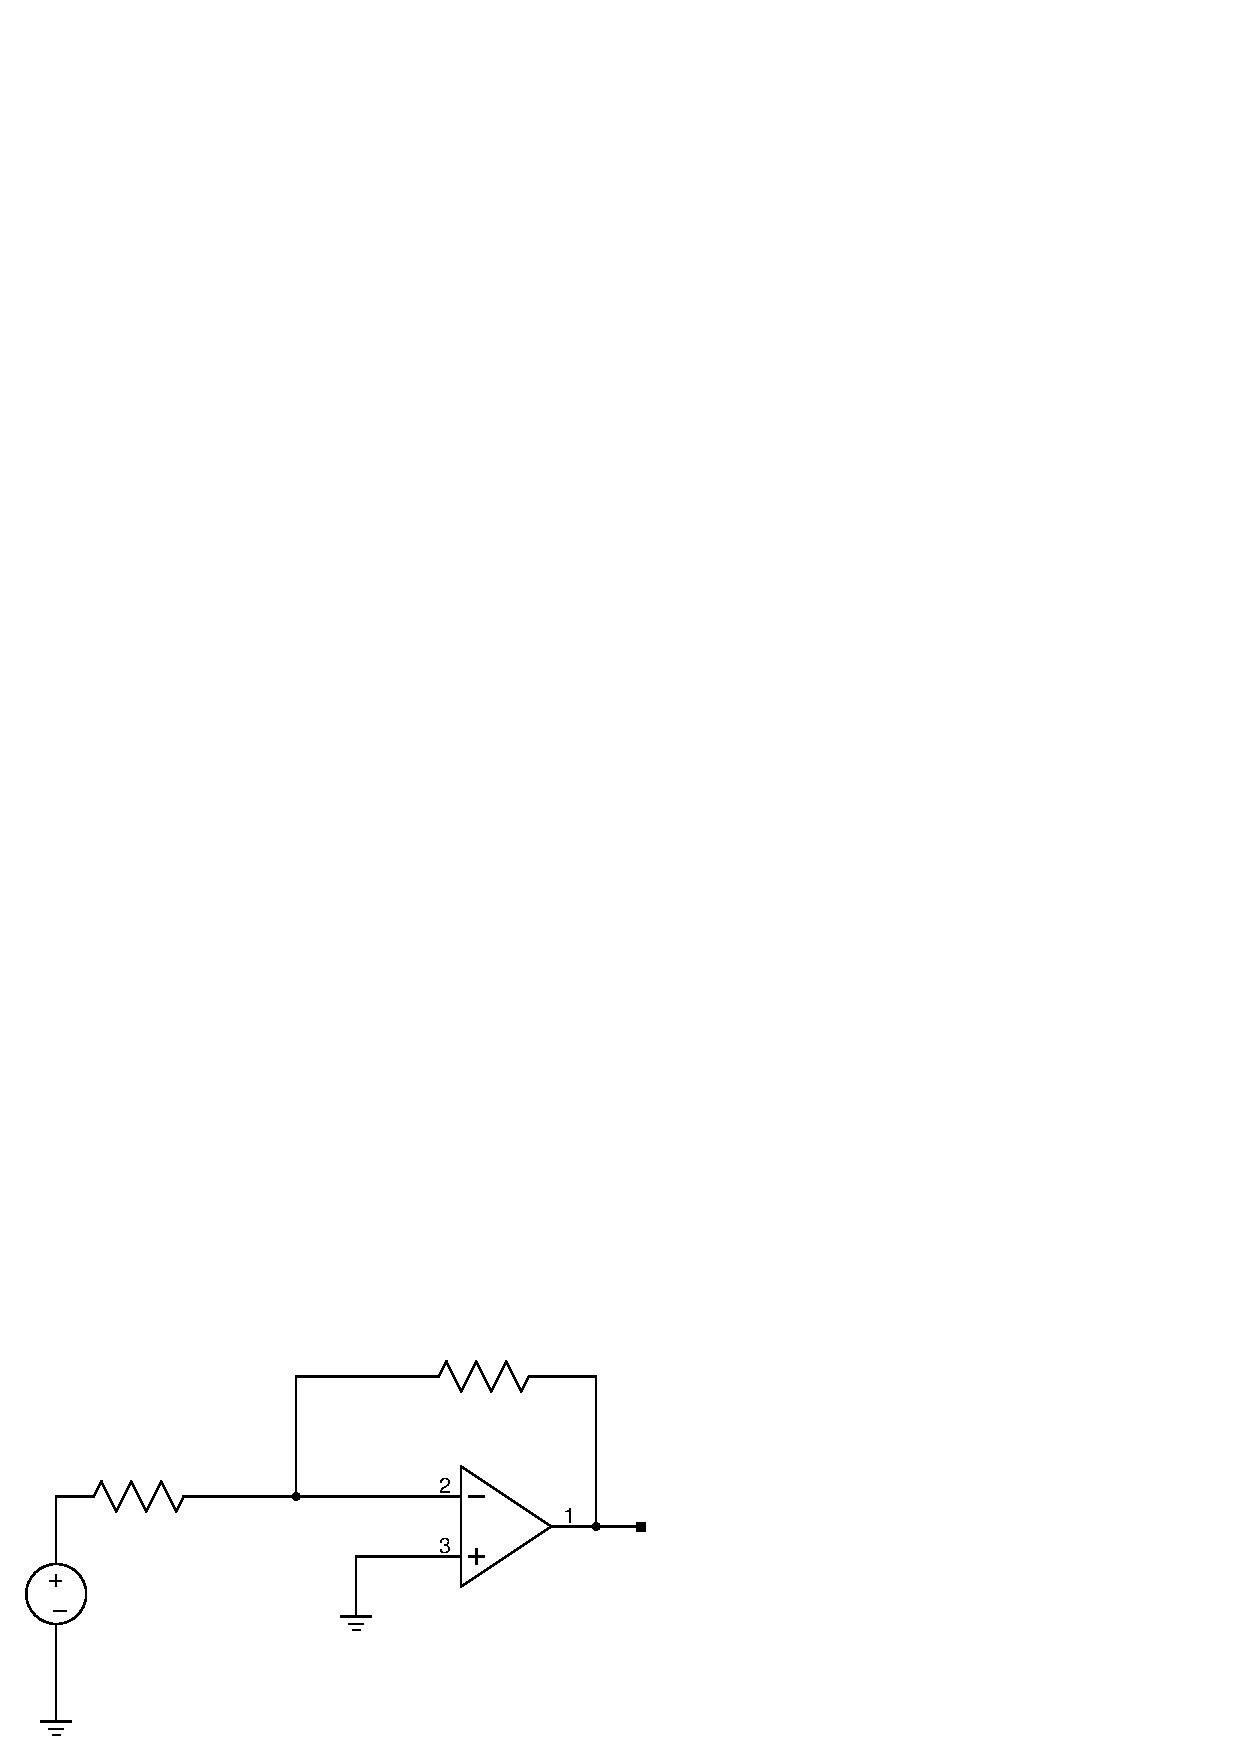
\includegraphics[scale=0.90]{invertingAmplifier}
\caption{منفی ایمپلیفائر}
\label{شکل_منفی_ایمپلیفائر}
\end{figure}
شکل میں حسابی ایمپلیفائر کے داخلی سروں پر برقی دباو کو \عددی{v_k}  اور \عددی{v_n} جبکہ خارجی سرے پر برقی دباو کو \عددی{v_o} کہا گیا ہے۔اس کتاب میں یہی علامتیں استعمال کی جائیں گی۔اس دور کو \اصطلاح{منفی ایمپلیفائر}\فرہنگ{منفی ایمپلیفائر}\فرہنگ{amplifier!inverting}\حاشیہب{inverting amplifier}  کہتے ہیں۔

ایسے  ادوار حل کرنے کی خاطر ہم حسابی ایمپلیفائر کے داخلی سروں پر \اصطلاح{کرخوف کے قوانین}\فرہنگ{کرخوف کے قوانین}\حاشیہب{Kirchoff's laws}  کا سہارا لیتے ہیں۔\اصطلاح{جوڑ}\فرہنگ{جوڑ}\حاشیہب{node}  \عددی{v_n} سے تین شاخیں نکلتی ہیں۔شکل میں ان شاخوں میں برقی رو کو \عددی{i_1} ، \عددی{i_2} اور \عددی{i_3} کہا گیا ہے۔کرخوف کا قانون برائے برقی رو\حاشیہب{Kirchoff's current law}  کہتا ہے کہ کسی بھی جوڑ پر اندر کی جانب کل برقی رو اس جوڑ پر باہر کی جانب کل برقی رو کے برابر ہو گی۔چونکہ ہم نے جوڑ پر تمام برقی رو کو باہر کی جانب نکلتے تصور کیا ہے لہٰذا اس صورت میں ان کا مجموعہ صفر ہو گا یعنی
\begin{align} \label{مساوات_منفی_منفی_مداخل_کے_جوڑ_پر_رو}
i_1+i_2+i_3 = 0
\end{align}
مساوات \حوالہ{مساوات_حسابی_بنیادی_پہلو}  کے تحت حسابی ایمپلیفائر کے داخلی سرے پر برقی رو کی قیمت صفر ہوتی ہے۔اس مثال میں اس برقی رو کو \عددی{i_3} کہا گیا ہے لہٰذا
\begin{align} \label{مساوات_حسابی_منفی_سرے_پر_صفر_رو}
i_3=0
\end{align}
ہے۔اُوہم کا قانون استعمال کرتے ہم \عددی{i_1} اور \عددی{i_2} حاصل کرتے ہیں۔
\begin{gather} 
\begin{aligned}\label{مساوات_منفی_بقایا_داخلی_رو}
i_1& =\frac{v_n-v_s}{R_1}\\
i_2 &=\frac{v_n-v_o}{R_2}
\end{aligned}
\end{gather}
مساوات \حوالہ{مساوات_حسابی_منفی_سرے_پر_صفر_رو}  اور \حوالہ{مساوات_منفی_بقایا_داخلی_رو}  کو مساوات \حوالہ{مساوات_منفی_منفی_مداخل_کے_جوڑ_پر_رو}  میں استعمال کرتے حاصل ہوتا ہے
\begin{align} \label{مساوات_منفی_کا_حصول}
\frac{v_n - v_s}{R_1}+\frac{v_n-v_o}{R_2}+0=0
\end{align}
	جوڑ \عددی{v_n} پر کرخوف کا قانون برائے برقی رو استعمال کرتے ہم نے مساوات \حوالہ{مساوات_منفی_کا_حصول}  حاصل کی۔اگر جوڑ \عددی{v_k} پر بھی برقی ارکان مثلاً مزاحمتیں یا برقی اشارات جڑے ہوتے، تب اس جوڑ کو بھی بالکل جوڑ \عددی{v_n} کی طرح حل کرتے۔موجودہ مثال میں ایسا نہیں۔جوڑ \عددی{v_k} \اصطلاح{برقی زمین}\فرہنگ{برقی!زمین}\حاشیہب{ground} کے ساتھ جڑا ہے اور یوں ہم اس جوڑ کے لئے لکھ سکتے ہیں
\begin{align} \label{مساوات_منفی_مثبت__زمین_پر}
v_k=0
\end{align}
	حسابی ایمپلیفائر کے دونوں داخلی برقی سروں والے جوڑوں کے لئے یوں مساواتیں حاصل کرنے کے بعد ہم مساوات \حوالہ{مساوات_حسابی_بنیادی_پہلو}  کی پہلی شِق استعمال کرتے ہیں۔مساوات \حوالہ{مساوات_منفی_مثبت__زمین_پر}  سے \عددی{v_k} کی قیمت کو مساوات \حوالہ{مساوات_منفی_کا_حصول}  میں \عددی{v_n} میں استعمال کرتے حل کرتے ہیں۔
\begin{align}
& \frac{0-v_s}{R_1}+\frac{0-v_o}{R_2}=0 \nonumber \\
& -\frac{v_s}{R_1}-\frac{v_o}{R_2}=0 \nonumber \\
& v_o =-\frac{R_2}{R_1} v_s
\end{align}
اس مساوات کو عموماً یوں لکھا جاتا ہے۔
\begin{align} \label{مساوات_منفی_افزائش}
A_v=\frac{v_o}{ v_s}=- \frac{R_2}{R_1}
\end{align}
	یہ مساوات شکل \حوالہ{شکل_منفی_ایمپلیفائر}  میں دیے \اصطلاح{منفی ایمپلیفائر} کے خارجی اشارہ \عددی{v_o}  اور مہیا کردہ داخلی اشارہ \عددی{v_s} کا تعلق بیان کرتا ہے۔اس مساوات میں \عددی{v_o} اور \عددی{v_s} کے کسر کو منفی ایمپلیفائر کے \اصطلاح{برقی دباو کی افزائش}\فرہنگ{افزائش!برقی دباو}\فرہنگ{voltage gain}\حاشیہب{voltage gain} \عددی{A_v} کہا گیا ہے۔اس اصطلاح کو عموماً چھوٹا کر کے \اصطلاح{منفی افزائش} یا صرف \اصطلاح{افزائش}\فرہنگ{افزائش}\فرہنگ{gain}\حاشیہب{gain} کہا جاتا ہے۔اس مساوات میں منفی کی علامت اس حقیقت کو بیان کرتا ہے کہ خارجی اور داخلی اشارے آپس میں \عددی{\SI{180}{\degree}} کے زاویہ پر ہیں۔

%=======================
\ابتدا{مثال}\شناخت{مثال_حسابی_غیر_خطی_کردار}
شکل \حوالہ{شکل_منفی_ایمپلیفائر} میں دکھلائے منفی ایمپلیفائر میں \عددی{R_1 = \SI{1}{\kilo \ohm}} اور \عددی{R_2 =\SI{10}{\kilo \ohm}} تصور کریں۔اس منفی ایمپلیفائر کو باری باری مندرجہ ذیل برقی اشارات بطور \عددی{v_s} مہیا کیا جاتا ہے۔ان تمام کے لئے حسابی دور کا خارجی اشارہ \عددی{v_o} حاصل کریں۔حل کرتے وقت \عددی{V_{CC}=\SI{+15}{\volt}} اور \عددی{V_{EE}=\SI{-15}{\volt}} تصور کریں۔
\begin{enumerate}
\item $\begin{aligned}[t]
v_s = \SI{0.2}{\volt}
\end{aligned}$
\item $\begin{aligned}[t]
v_s = \SI{0.31}{\volt}
\end{aligned}$

\item $\begin{aligned}[t]
v_s = \SI{-0.52}{\volt}
\end{aligned}$

\item $\begin{aligned}[t]
v_s = 0.1 \sin \left (t \right )
\end{aligned}$

\item $\begin{aligned}[t]
v_s = 2 \sin \left ( t \right )
\end{aligned}$
\end{enumerate}
حل:	جب تک خارجی اشارہ \عددی{v_o} مساوات \حوالہ{مساوات_حسابی_کے_خارجی_حدود}  میں دیے حدود کے اندر رہتا ہے، اس وقت تک مساوات \حوالہ{مساوات_منفی_افزائش}  منفی ایمپلیفائر کی خارجی اشارہ \عددی{v_o} حاصل کرنے کے لئے استعمال ہو گا یعنی
\begin{align*}
v_o = - \left ( \frac{R_2}{R_1} \right ) v_s = -\left ( \frac{10000}{1000} \right ) v_s=-10 v_s
\end{align*}
%
\begin{enumerate}
\item
$\begin{aligned}
v_o = -10 \times 0.2 = \SI{-2}{\volt}
\end{aligned}$

\item
$\begin{aligned}
v_o = -10 \times 0.31 = \SI{-3.1}{\volt}
\end{aligned}$

\item
$\begin{aligned}
v_o = -10 \times \left(-0.52 \right ) = \SI{5.2}{\volt}
\end{aligned}$

\item
$\begin{aligned}
v_o = -10 \times 0.1 \sin (t) = - \sin(t) 
\end{aligned}$

\item
$\begin{aligned}
v_o = -10 \times 2 \sin(t)=\underbrace{-20 \sin(t)}_{\text{\RL{غیر خطی خطہ}}}
\end{aligned}$
\end{enumerate}

		اس مثال کی پہلی چار صورتوں میں مساوات \حوالہ{مساوات_منفی_افزائش}  سے صحیح جواب حاصل ہوتا ہے۔آخری صورت میں چونکہ حاصل \عددی{v_o} کی قیمت حسابی ایمپلیفائر کے خطی حدود سے تجاوز کرتی ہے لہٰذا اس جواب کو رد کیا جاتا ہے۔اس جواب کے نیچے غیر خطی خطہ لکھ کر اسی بات کی وضاحت کی گئی ہے۔اس صورت میں \عددی{t} کی قیمت تبدیل کرتے \عددی{v_o} کی قیمت \عددی{v_o = -20 \sin(t)} سے ہی حاصل کی جاتی ہے۔جب تک حاصل جواب مساوات \حوالہ{مساوات_حسابی_کے_خارجی_حدود}  میں دیے حدود کے اندر رہے اسے صحیح تصور کیا جاتا ہے۔جہاں \عددی{v_o}  کی قیمت \عددی{V_{CC}}سے بلند ہونے کی کوشش کرے وہاں \عددی{v_o=V_{CC}} لیا جاتا ہے۔اسی طرح جہاں \عددی{v_o} کی قیمت \عددی{V_{EE}} سے تجاوز کرے وہاں \عددی{v_o = V_{EE}} لیا جاتا ہے۔اس بات کی وضاحت شکل \حوالہ{شکل_حسابی_لبریز} میں کی گئی ہے۔اس شکل کی مدد سے آپ دیکھ سکتے ہیں کہ حسابی ایمپلیفائر \عددی{V_{EE}} تا \عددی{V_{CC}} کے حدود میں خطی رد عمل رکھتا ہے جبکہ ان حدود کے باہر یہ غیر خطی رد عمل رکھتا ہے جس سے خارجی اشارہ  تراشا جاتا ہے۔
\begin{figure}
\centering

\includegraphics[scale=0.90]{clippedSineWave}
\caption{حسابی ایمپلیفائر کے لبریز ہونے سے خارجی اشارہ  تراشا جاتا ہے}
\label{شکل_حسابی_لبریز}
\end{figure}
\انتہا{مثال}

%============

	اس مثال میں آپ نے دیکھا کہ \عددی{v_s} کے مثبت ہونے کی صورت میں\عددی{v_o} کی قیمت منفی ہوتی ہے جبکہ \عددی{v_s} کے منفی ہونے کی صورت میں \عددی{v_o}کی قیمت مثبت ہوتی ہے یعنی منفی ایمپلیفائر مہیا کردہ داخلی اشارے \عددی{v_s} کی قیمت کو اُلٹ کرتا ہے۔اسی لئے اسے \اصطلاح{منفی ایمپلیفائر}\حاشیہب{inverting amplifier}\فرہنگ{منفی ایمپلیفائر}\فرہنگ{amplifier!inverting}  کہا جاتا ہے۔

	اسی مثال میں آپ نے دیکھا کہ \عددی{v_o} کی قیمت \عددی{v_s} کے منفی دس \عددی{-10} گنا ہے یعنی یہ دور مہیا کردہ اشارہ کے حیطہ کو بڑھا کر خارج کرتا ہے۔اس مثال میں منفی ایمپلیفائر کی  برقی دباو کی افزائش کی قیمت \عددی{-10} ہے۔منفی ایمپلیفائر کی افزائش مساوات \حوالہ{مساوات_منفی_افزائش}  سے حاصل ہوتی ہے۔

\begin{figure}
\centering
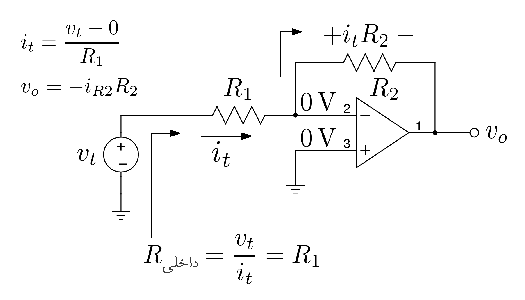
\includegraphics[scale=0.90]{invertingAmplifierInputResistance}
\caption{منفی حسابی ایمپلیفائر کی داخلی مزاحمت}
\label{شکل_حسابی_منفی_داخلی_مزاحمت}
\end{figure}
\ابتدا{مثال} \شناخت{مثال_حسابی_خطی_غیر_خطی_خطے}
مثال \حوالہ{مثال_حسابی_غیر_خطی_کردار} کے پہلے اجزاء میں ایمپلیفائر خطی خطے میں رہتا ہے جبکہ آخری جزو میں یہ غیر خطی خطے میں داخل ہوتا ہے۔انہیں پر مزید غور کرتے ہیں۔\عددی{v_s=\SI{0.52}{\volt}} اور  \عددی{v_s=\SI{2}{\volt}} کی صورت میں \عددی{v_n} حاصل کریں۔

حل:
پہلی صورت میں \عددی{v_o=\SI{-5.2}{\volt}} اور دوسری صورت میں \عددی{v_o=\SI{-15}{\volt}} ہوں گے۔جوڑ \عددی{v_n} پر کرخوف کے قانون برائے برقی رو سے
\begin{align*}
\frac{v_n -v_s}{R_1}+\frac{v_n-v_o}{R_2}=0\\
v_n=\frac{v_s R_2+v_o R_1}{R_1+R_2}
\end{align*}
حاصل ہوتا ہے لہٰذا پہلی صورت میں \عددی{v_n=\SI{0}{\volt}} جبکہ دوسری صورت میں \قریب{\عددی{v_n=\SI{0.45}{\volt}}} ہوں گے۔دونوں صورتوں میں مثبت داخلی سرا برقی زمین کے ساتھ جڑا ہے لہٰذا \عددی{v_k=\SI{0}{\volt}} رہتا ہے۔

آپ دیکھ سکتے ہیں کہ جب تک ایمپلیفائر خطی خطے میں رہے \عددی{v_n=v_k} رہتا ہے جبکہ غیر خطی خطے میں داخل ہوتے ہی \عددی{v_n \ne v_k} ہو جاتا ہے۔
\begin{align}
v_d &=0   \hspace{5mm} \text{\RL{خطی خطہ}}\\
v_d & \ne 0 \hspace{5mm} \text{\RL{غیر خطی خطہ}}
\end{align}
\انتہا{مثال}

منفی حسابی ایمپلیفائر کا داخلی مزاحمت \سیدھازیرنوشت{R}{داخلی} حاصل کرنے کی خاطر شکل \حوالہ{شکل_حسابی_منفی_داخلی_مزاحمت} سے رجوع کریں۔داخلی مزاحمت حاصل کرنے کی خاطر دور پر \عددی{v_t} لاگو کرتے ہوئے \عددی{i_t} ناپا جاتا ہے۔ان دو مقداروں کی شرح  کو داخلی مزاحمت کہا جاتا ہے یعنی
\begin{align*}
R_{\textup{داخلی}}=\frac{v_t}{i_t}
\end{align*}
چونکہ جوڑ \عددی{v_k} برقی زمین کے ساتھ جڑا ہے لہٰذا \عددی{v_k=0} ہو گا اور یوں \عددی{v_n} بھی صفر وولٹ پر ہو گا۔اس طرح \عددی{R_1} کا دایاں سرا صفر وولٹ پر ہے جبکہ اس کے بائیں سرے پر \عددی{v_t} لاگو کیا گیا ہے لہٰذا \عددی{i_t=\tfrac{v_t}{R_1}} ہو گا۔اس قیمت کو مندرجہ بالا مساوات میں استعمال کرتے  ہوئے
\begin{align}
R_{\textup{داخلی}}=R_1
\end{align}
حاصل ہوتا ہے۔جیسا شکل میں دکھایا گیا ہے، مزاحمت \عددی{R_1} سے گزرتی برقی رو \عددی{i_t} جوڑ \عددی{v_n} پر صرف \عددی{R_2} کے جانب جا سکتی ہے۔یوں \عددی{R_2} میں بھی \عددی{i_t} برقی رو پائی جائے گی جس سے اس مزاحمت کے دو سروں کے درمیان \عددی{i_t R_2} برقی دباو پیدا ہو گا۔چونکہ \عددی{R_2} کا بایاں سرا صفر وولٹ پر ہے لہٰذا اس کا دایاں سرا یعنی جوڑ \عددی{v_o} پر \عددی{-i_t R_2} برقی دباو پایا جائے گا۔اس طرح
\begin{align*}
v_o=-i_t R_2 =-\frac{v_t}{R_1} R_2
\end{align*}
ہو گا جس سے منفی حسابی ایمپلیفائر کی جانی پہچانی مساوات
\begin{align}
A_v=\frac{v_o}{v_t}=-\frac{R_2}{R_1}
\end{align}
حاصل ہوتی ہے۔

منفی حسابی ایمپلیفائر کی افزائش برقرار رکھتے ہوئے اس کے داخلی مزاحمت کو بڑھانے کی خاطر \عددی{R_1} کی قیمت بڑھانی ہو گی۔چونکہ \عددی{A_v=-\tfrac{R_2}{R_1}} ہے لہٰذا \عددی{R_1} بڑھاتے وقت \عددی{R_2} کی قیمت بھی بڑھانی ہو گی۔کبھی کبھار \عددی{R_2} کی قیمت اتنی بڑھ جاتی ہے کہ اس سے دیگر مسائل پیدا ہوتے ہیں۔آئیں دیکھیں کہ ایسی صورت حال سے کیسے نپٹا جا سکتا ہے۔

\ابتدا{مثال} \شناخت{مثال_حسابی_منفی_زیادہ_داخلی_مزاحمت}
شکل \حوالہ{شکل_حسابی_منفی_داخلی_زیادہ_مزاحمت} میں دکھائے دور کی افزائش حاصل کریں۔

حل:
\عددی{v_k=0} کی وجہ سے \عددی{v_n=0} ہے لہٰذا \عددی{i_1=\tfrac{v_s}{R_1}} ہو گا۔\عددی{i_1} جوڑ \عددی{v_n} پر \عددی{R_2} کے جانب مڑ جائے گی۔یوں \عددی{i_2=i_1} ہو گا جس سے \عددی{v_1=-i_1 R_2} یعنی
\begin{align*}
v_1=-\frac{R_2}{R_1} v_s
\end{align*}
اور
\begin{align*}
i_3=\frac{0-v_1}{R_3}=\frac{R_2}{R_1 R_3} v_s
\end{align*}
ہوں گے۔\عددی{i_4=i_2+i_3} یعنی
\begin{align*}
i_4=\frac{v_s}{R_1}+\frac{R_2}{R_1 R_3} v_s=\left(1+\frac{R_2}{R_3} \right) \frac{v_s}{R_1}
\end{align*}
ہو گا جو مزاحمت \عددی{R_4} میں سے گزرتے ہوئے اس پر \عددی{i_4 R_4} برقی دباو پیدا کرے گا۔یوں
\begin{align*}
v_1-v_o=i_4 R_4=\left(1+\frac{R_2}{R_3} \right) \frac{R_4 v_s}{R_1}
\end{align*}
\عددی{v_1} کی قیمت کے استعمال سے
\begin{align*}
-\frac{R_2}{R_1} v_s-v_o=\left(1+\frac{R_2}{R_3} \right) \frac{R_4 v_s}{R_1}
\end{align*}
یعنی
\begin{align} \label{مساوات_حسابی_داخلی_مزاحمت_بڑھایا_گیا}
A_v=\frac{v_o}{v_s}=-\frac{R_2}{R_1}\left[1+\left(\frac{1}{R_2}+\frac{1}{R_3} \right)R_4 \right]
\end{align}
حاصل ہوتا ہے۔

\begin{figure}
\centering
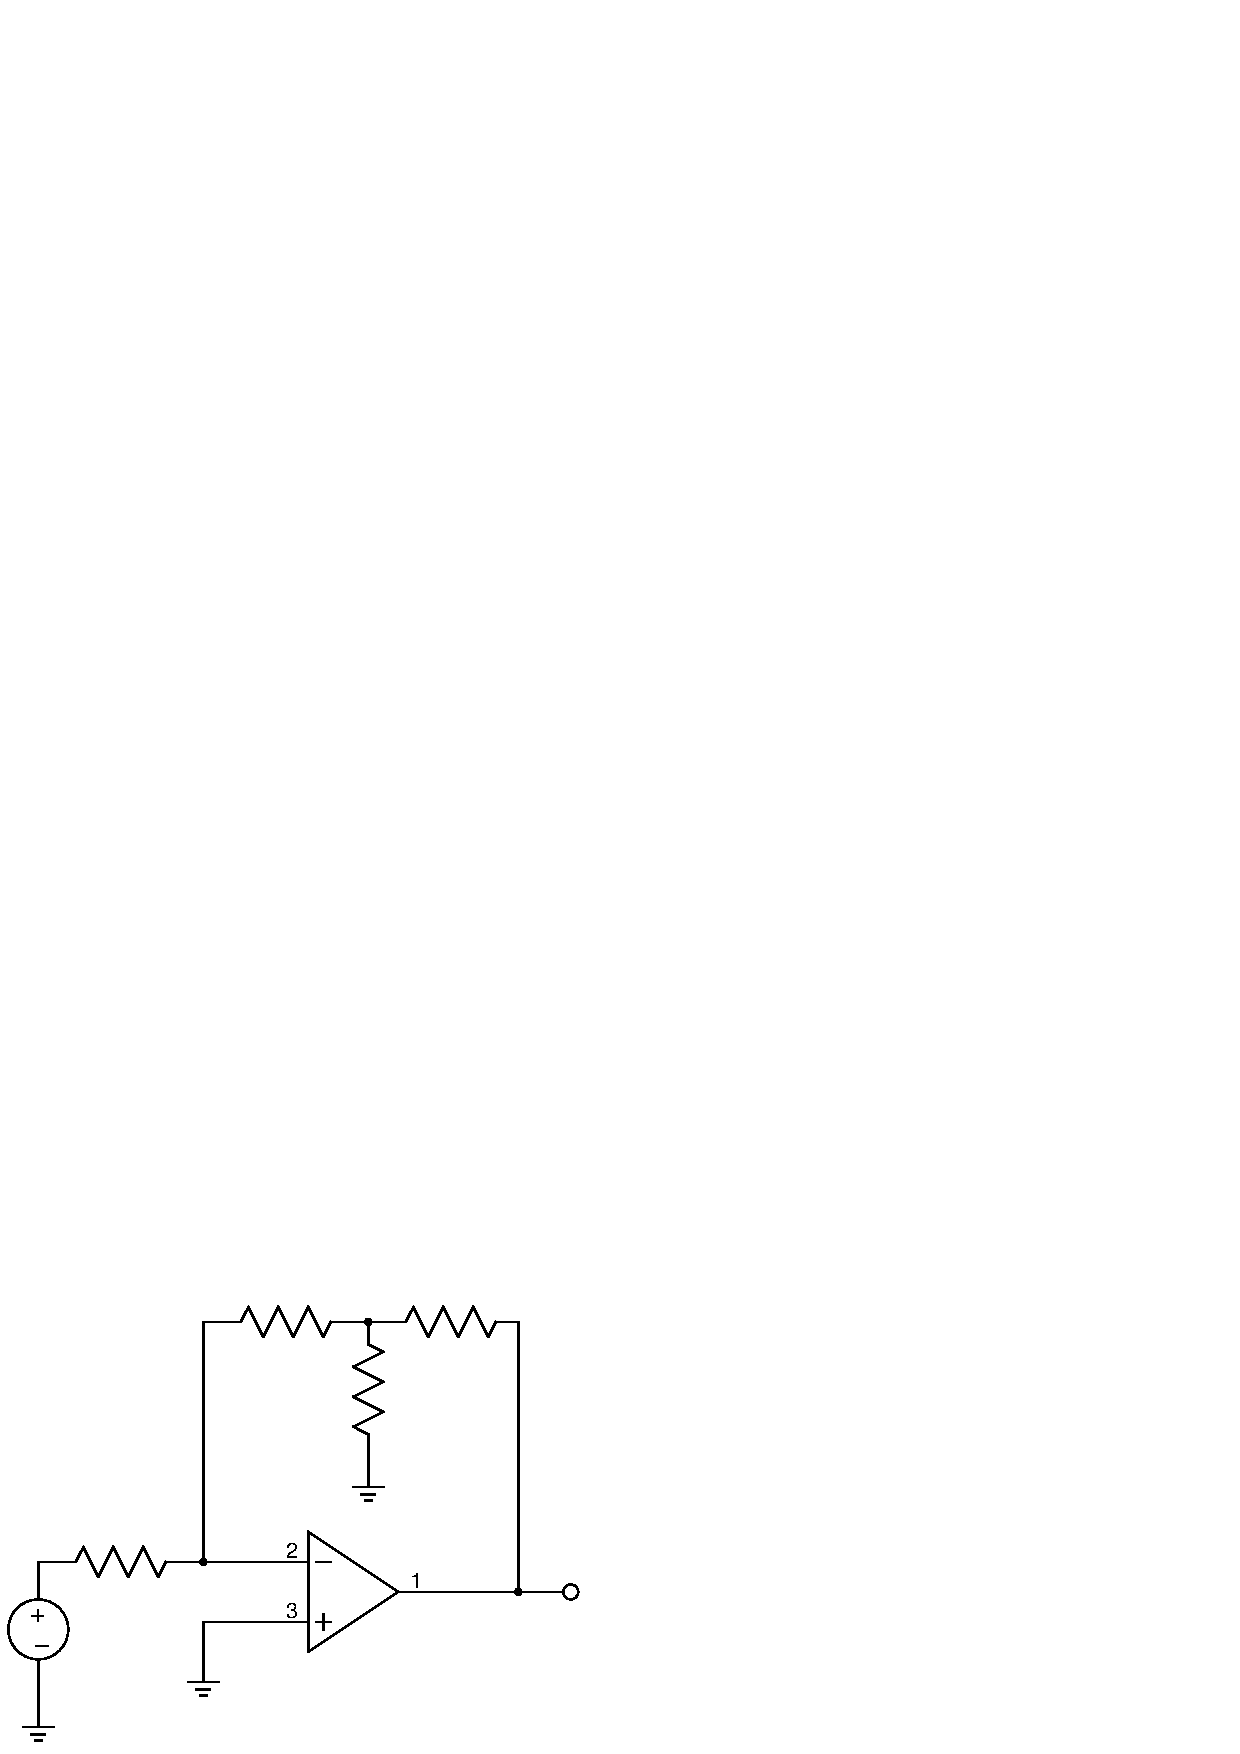
\includegraphics[scale=0.90]{invertingAmplifierIncreasedInputResistance}
\caption{منفی حسابی ایمپلیفائر کا داخلی مزاحمت بڑھایا گیا ہے}
\label{شکل_حسابی_منفی_داخلی_زیادہ_مزاحمت}
\end{figure}

اس ایمپلیفائر کے داخلی مزاحمت کی قیمت \عددی{R_1} ہے۔
\انتہا{مثال}

اس مثال کے نتائج مد نظر رکھتے ہوئے ہم دیکھتے ہیں کہ داخلی مزاحمت بڑھانے کی خاطر اگر \عددی{R_1} کی قیمت بڑھائی جائے تو افزائش برقرار رکھنے کی خاطر یہ ضروری نہیں کہ \عددی{R_2}  کی قیمت بھی بڑھائی جائے۔ہم  \عددی{R_3} اور \عددی{R_4} کے قیمتیں ایسی رکھ سکتے ہیں کہ درکار افزائش حاصل کی جائے۔یہ بات خصوصی  طور پر غور طلب ہے کہ \عددی{R_3} کے قیمت کو کم کرتے ہوئے افزائش بڑھائی جا سکتی ہے لہٰذا \عددی{R_1} کی قیمت زیادہ سے زیادہ رکھتے ہوئے داخلی مزاحمت بڑھائی جا سکتی ہے۔ 

\ابتدا{مثال}
شکل \حوالہ{شکل_حسابی_منفی_داخلی_زیادہ_مزاحمت} میں داخلی مزاحمت \عددی{\SI{300}{\kilo \ohm}} جبکہ \عددی{A_v=\SI{-100}{\volt\per \volt}} درکار ہے۔ تمام مزاحمت حاصل کریں۔

حل:
داخلی مزاحمت  کی شرط کی وجہ سے \عددی{R_1=\SI{300}{\kilo \ohm}} رکھی جاتی ہے۔ ایسی صورت میں \عددی{R_2} اور \عددی{R_4} کو بھی \عددی{\SI{300}{\kilo \ohm}} ہی رکھتے ہوئے \عددی{R_3} کی قیمت مساوات  \حوالہ{مساوات_حسابی_داخلی_مزاحمت_بڑھایا_گیا} سے \عددی{\SI{3061}{\ohm}}حاصل ہوتی ہے۔  
\انتہا{مثال}
%=============

مزاحمت کو اس کے قیمت سے پکارا جاتا ہے۔یوں \عددی{\SI{1}{\kilo \ohm}} قیمت کے مزاحمت کو \عددی{\SI{1}{\kilo \ohm}} کا مزاحمت پکارا جائے گا۔\عددی{\SI{\mp 5}{\percent}} مزاحمت سے مراد ایسا مزاحمت ہے جس کی قیمت پکارے قیمت سے  پانچ فی صد زیادہ یا کم ممکن ہے۔یوں 
\عددی{\SI{1}{\kilo \ohm} \mp \SI{5}{\percent}} مزاحمت کی قیمت \عددی{\SI{0.95}{\kilo \ohm}} تا \عددی{\SI{1.05}{\kilo \ohm}} ممکن ہے۔\عددی{\SI{1}{\kilo \ohm}} کو مزاحمت کی \اصطلاح{پکاری گئی قیمت}\فرہنگ{پکاری گئی قیمت}\حاشیہب{nominal value} جبکہ  \عددی{\SI{\mp 5}{\percent}} کو قیمت میں \اصطلاح{غلطی}\فرہنگ{مزاحمت میں غلطی}\حاشیہب{tolerance} کہا جاتا ہے۔

مزاحمت \عددی{R} کی قیمت \عددی{\SI{5}{\percent}} بڑھنے سے \عددی{\tfrac{5}{100}R} بڑھ کر \عددی{\left(1+0.05 \right) R} ہو جائے گی۔اسی طرح \عددی{R} کی قیمت \عددی{\SI{5}{\percent}} کم ہونے سے  \عددی{\left(1-0.05 \right) R} ہو جائے گی۔ان دو قیمتوں کو ہم \عددی{\left(1+\epsilon \right)R} اور \عددی{\left(1-\epsilon \right)R} لکھ سکتے ہیں جہاں \عددی{\epsilon=0.05} کے برابر ہے۔

\ابتدا{مثال}
\اصطلاح{منفی حسابی ایمپلیفائر} میں \عددی{R_2=\SI{47}{\kilo \ohm}} جبکہ \عددی{R_1=\SI{1}{\kilo \ohm}} رکھا گیا۔دونوں مزاحمتوں کے قیمت میں \عددی{\SI{\mp 5}{\percent}} غلطی کی گنجائش ہے۔اس ایمپلیفائر کے ممکنہ افزائش کے حدود حاصل کریں۔

حل:منفی حسابی ایمپلیفائر کی افزائش \عددی{A= -\tfrac{R_2}{R_1}} کے برابر ہے۔اس کا حتمی قیمت اس وقت کم سے کم  ہو گا جب \عددی{R_2} کی حقیقی قیمت \عددی{\SI{5}{\percent}} کم یعنی \عددی{\left(1-\epsilon \right) R_2} جبکہ \عددی{R_1} کی حقیقی قیمت \عددی{\SI{5}{\percent}} زیادہ  یعنی \عددی{\left(1+\epsilon \right) R_2} ہو جہاں \عددی{\epsilon=0.05} کے برابر ہے۔اسی طرح افزائش کی زیادہ سے زیادہ قیمت اس وقت حاصل ہو گی جب \عددی{R_2} کی حقیقی قیمت \عددی{\SI{5}{\percent}} زیادہ جبکہ \عددی{R_1} کی حقیقی قیمت \عددی{\SI{5}{\percent}} کم ہو۔یوں
\begin{align*}
A_{\text{کمتر}}=-\frac{1-\epsilon}{1+\epsilon} \left(\frac{R_2}{R_1} \right)=-\frac{0.95}{1.05} \left(\frac{47000}{1000}\right)=-42.524\\
A_{\text{بلندتر}}=-\frac{1+\epsilon}{1-\epsilon} \left(\frac{R_2}{R_1} \right)=-\frac{1.05}{0.95} \left(\frac{47000}{1000}\right)=-51.947
\end{align*}
\انتہا{مثال}

اس مثال میں آپ نے دیکھا کہ مزاحمتوں کے قیمت میں \اصطلاح{غلطی کے گنجائش} کی وجہ سے افزائش کی قیمت درکار قیمت سے انحراف کر سکتی ہے۔موجودہ مثال میں ایمپلیفائر کے افزائش کی پکاری گئی قیمت \عددی{\SI{-47}{\volt \per \volt}} ہے جبکہ حقیقت میں یہ \عددی{\SI{-42.524}{\volt \per \volt}} تا \عددی{\SI{-51.947}{\volt \per \volt}} کے درمیان کہیں پر بھی ہو سکتی ہے۔یوں حقیقی افزائش، پکاری گئی قیمت سے
\begin{align*}
\abs{\frac{51.947-47}{47} \times 100} \approx \SI{10}{\percent}
\end{align*}
زیادہ یا کم ممکن ہے۔

%==================
\ابتدا{مثال}
شکل \حوالہ{شکل_حسابی_مزاحمت_نما_ایمپلیفائر} میں دکھائے دور کا داخلی مزاحمت، خارجی مزاحمت اور \اصطلاح{مزاحمت نما افزائش}\فرہنگ{مزاحمت نما افزائش}\حاشیہب{transconductance gain}\فرہنگ{transconductance gain} \عددی{R_m=\tfrac{v_o}{i_s}} حاصل کریں۔اس دور کو استعمال کرتے ہوئے برقی رو اشارے \عددی{i_s} سے برقی دباو کا اشارہ \عددی{v_o} حاصل کیا جاتا ہے۔ 
\begin{figure}
\centering
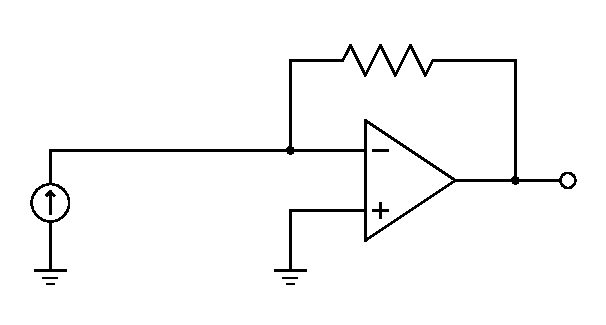
\includegraphics[scale=0.90]{opampTransconductanceAmplifier}
\caption{حسابی مزاحمت نما ایمپلیفائر}
\label{شکل_حسابی_مزاحمت_نما_ایمپلیفائر}
\end{figure}

حل:جوڑ \عددی{v_k} برقی زمین کے ساتھ جڑا ہے لہٰذا \عددی{v_k=0} اور یوں \عددی{v_n=0} ہو گا۔داخلی جانب برقی رو \عددی{i_s} جبکہ برقی دباو \عددی{v_n} ہے لہٰذا
\begin{align*}
R_{\textup{داخلی}}=\frac{v_n}{i_s}=\frac{0}{i_s}=\SI{0}{\ohm}
\end{align*}
حاصل ہوتا ہے۔

خارجی مزاحمت حاصل کرنے کی خاطر کامل حسابی ایمپلیفائر کا دور جسے شکل \حوالہ{شکل_کامل_حسابی_ایمپلیفائر_کا_مساوی_دور} میں دکھایا گیا ہے کو زیر استعمال لاتے ہیں۔\عددی{v_d=0} ہونے کی صورت میں اس کے خارجی جانب صفر اُوہم حاصل ہوتا ہے لہٰذا
\begin{align*}
R_{\textup{خارجی}}=\SI{0}{\ohm}
\end{align*}
حاصل ہوتا ہے۔

آئیں اب مزاحمت نما افزائش \عددی{R_m} حاصل کریں۔جیسے شکل میں دکھایا گیا ہے، جوڑ \عددی{v_n} پر آمد برقی رو \عددی{i_s} صرف مزاحمت \عددی{R} کی جانب جا سکتی ہے۔یوں اس مزاحمت پر \عددی{i_s R} برقی دباو پیدا ہو گا۔مزاحمت کا بایاں سرا برقی زمین پر ہے لہٰذا
\begin{align*}
v_o=-i_s R\\
R_m=\frac{v_o}{i_s}=-R
\end{align*}
ہو گا۔
\انتہا{مثال}

حسابی منفی ایمپلیفائر کو شکل \حوالہ{شکل_حسابی_واپسی_منفی_ایمپلیفائر} الف میں دوبارہ دکھایا گیا ہے جبکہ شکل  الف     میں اسی کو قدر مختلف طرز پر بنایا گیا ہے۔شکل  الف     میں یہ بات کھل کر سامنے آتی ہے کہ خارجی اشارہ \عددی{v_o} کو بھی بطور داخلی اشارہ استعمال کیا جا رہا ہے۔
\begin{figure}
\centering
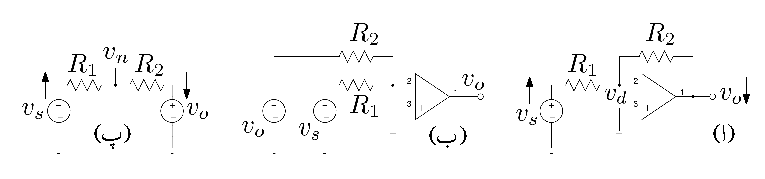
\includegraphics[scale=0.90]{feedbackInvertingAmplifier}
\caption{واپسی حسابی منفی ایمپلیفائر}
\label{شکل_حسابی_واپسی_منفی_ایمپلیفائر}
\end{figure}

ایسے ادوار جن میں خارجی اشارہ کو بطور داخلی اشارہ استعمال کیا گیا ہو کو \اصطلاح{واپسی ادوار}\فرہنگ{واپسی ادوار}\حاشیہب{feedback circuits} کہتے ہیں اور جن خارجی  اشارات کو یوں بطور داخلی اشارات استعمال کیا گیا ہو انہیں \اصطلاح{واپسی اشارات}\فرہنگ{واپسی اشارات}\حاشیہب{feedback signals}\فرہنگ{feedback signal}  کہتے ہیں۔یوں منفی ایمپلیفائر \اصطلاح{واپسی ادوار} کی ایک مثال ہے۔

حسابی ایمپلیفائر کے تفرقی افزائش برقی دباو \عددی{A_d}  کی قیمت لامحدود ہونے کے وجہ سے نہایت کم داخلی اشارے پر بھی اس کو غیر خطی خطے میں داخل ہونا چاہیے۔حقیقت میں ایمپلیفائر استعمال ہی خطی خطے میں ہوتا ہے اور واپسی اشارے کی شمولیت اس کو ممکن بناتی ہے۔

حسابی منفی ایمپلیفائر پر دوبارہ غور کریں۔داخلی اشارہ \عددی{v_s} کو منفی داخلی سرے پر مہیا کیا گیا ہے۔جیسا شکل میں تیر کے نشانوں سے دکھایا گیا ہے کہ اگر داخلی اشارہ \عددی{v_s} کو مثبت جانب \عددی{(\uparrow)} لے جایا جائے تو خارجی اشارہ \عددی{v_o} منفی جانب \عددی{(\downarrow)} حرکت کرتا ہے۔ اسی طرح اگر داخلی اشارہ \عددی{v_s} کو منفی جانب \عددی{(\downarrow)} لے جایا جائے تو خارجی اشارہ \عددی{v_o} مثبت جانب  حرکت کرتا ہے۔منفی داخلی سرے  پر کرخوف کے قانون برائے برقی رو سے 
\begin{align}\label{مساوات_حسابی_واپسی_منفی}
\frac{v_n-v_s}{R_1}+\frac{v_n-v_o}{R_2}=0\\
v_0=\frac{R_2}{R_1} v_s
\end{align}
حاصل ہوتا ہے جہاں  دوسرے قدم پر \عددی{v_k=0} کی وجہ سے \عددی{v_n=0} کا استعمال کیا گیا۔اسی حقیقت کو یوں بھی دیکھا جا سکتا ہے کہ حسابی ایمپلیفائر \عددی{v_o} کو یوں رکھتا ہے کہ \عددی{v_d=0} یعنی \عددی{v_k=v_n}  حاصل ہو۔چونکہ منفی حسابی ایمپلیفائر میں \عددی{v_k=0} ہے لہٰذا حسابی ایمپلیفائر \عددی{v_o} کو یوں رکھے گا کہ \عددی{v_n=0} حاصل ہو۔شکل \حوالہ{شکل_حسابی_واپسی_منفی_ایمپلیفائر} پ میں \عددی{v_n} کی مساوات حاصل کرتے ہوئے  اس مساوات پر \عددی{v_n=0} کی شرط لاگو کریں۔ایسا کرنے سے مساوات \حوالہ{مساوات_حسابی_واپسی_منفی} ہی حاصل ہوتے ہیں۔
%---------------------
\ابتدا{مثال}
حسابی منفی ایمپلیفائر میں \عددیء{R_1=\SI{1}{\kilo \ohm}}، \عددیء{R_2=\SI{5}{\kilo \ohm}} لیتے ہوئے \عددیء{v_s=\SI{1}{\volt}}، \عددیء{v_s=\SI{1.5}{\volt}}  اور \عددیء{v_s=\SI{2}{\volt}}  پر \عددی{v_o} حاصل کریں۔تینوں جوابات کو استعمال کرتے ہوئے شکل \حوالہ{شکل_حسابی_واپسی_منفی_ایمپلیفائر} پ میں \عددی{v_n} کی قیمت حاصل کریں۔

حل:
ان داخلی اشارات پر
\begin{align*}
v_o&=-\left(\frac{5000}{1000}\right) \times 1=\SI{-5}{\volt}\\
 v_o&=-\left(\frac{5000}{1000}\right) \times 1.5=\SI{-7.5}{\volt}\\
v_o&=-\left(\frac{5000}{1000}\right) \times 2=\SI{-10}{\volt}
\end{align*}
حاصل ہوتے ہیں۔آئیں ہر داخلی-خارجی برقی دباو کے جوڑے کو استعمال کرتے ہوئے شکل \حوالہ{شکل_حسابی_واپسی_منفی_ایمپلیفائر} پ میں \عددی{v_n} حاصل کریں۔کرخوف کے قانون برائے برقی رو سے
\begin{align*}
\frac{v_n-v_s}{R_1}+\frac{v_n-v_o}{R_2}=0\\
v_n=\frac{R_2 v_s +R_1 v_o}{R_1+R_2}
\end{align*}
حاصل ہوتا ہے اور یوں
\begin{align*}
v_n&=\frac{5000 \times 1 +1000 \times (-5)}{1000+5000}=\SI{0}{\volt}\\
v_n&=\frac{5000 \times 1.5 +1000 \times (-7.5)}{1000+5000}=\SI{0}{\volt}\\
v_n&=\frac{5000 \times 2 +1000 \times (-10)}{1000+5000}=\SI{0}{\volt}
\end{align*}
حاصل ہوتے ہیں۔
\انتہا{مثال}

مندرجہ بالا مثال میں ہم نے دیکھا کہ \عددی{v_o} اس جانب حرکت کرتا ہے جس جانب \عددی{v_k-v_n} یعنی \عددی{v_d} کی قیمت صفر حاصل ہو۔وہ واپسی دور جس کا خارجی اشارہ، دور کے داخلی اشارے کے الٹ کام کرے کو \اصطلاح{منفی واپسی دور}\فرہنگ{منفی واپسی دور}\فرہنگ{feedback circuit!negative}\حاشیہب{negative feedback circuit} کہتے ہیں اور اس عمل کو \اصطلاح{منفی واپسی عمل} یا صرف \اصطلاح{منفی واپسی} کہتے ہیں۔اس باب میں \اصطلاح{منفی واپسی ادوار} حل کرنے پر غور کیا جائے گا۔\اصطلاح{مثبت واپسی} کا استعمال باب \حوالہ{باب_مرتعش} میں دیکھا جائے گا۔  
 
شکل \حوالہ{شکل_حسابی_مثبت_واپسی_دور} میں  \اصطلاح{مثبت واپسی دور} کی مثال دکھائی گئی ہے۔یہاں \عددی{v_s} حسابی ایمپلیفائر کے مثبت داخلی سرے  پر مہیا کیا گیا ہے۔یوں \عددی{v_s} بڑھانے سے \عددی{v_d} بڑھے گا اور یوں \عددی{v_o} بھی مثبت جانب بڑھے گا۔جیسے شکل  الف     میں دکھایا گیا ہے کہ \عددی{v_s} اور \عددی{v_o} دونوں بڑھنے سے \عددی{v_k} صرف بڑھ ہی سکتا ہے۔اگر \عددی{v_o} کو بطور واپسی اشارہ داخلی سرے  پر مہیا نہ کیا جاتا تب بھی \عددی{v_s} بڑھانے سے  \عددی{v_k} اور \عددی{v_d}بڑھتے لیکن \عددی{v_o} کا بطور واپسی اشارہ استعمال کرنے کی وجہ سے \عددی{v_k}   اور  \عددی{v_d} مزید زیادہ بڑھتے ہیں۔ایسے ادوار جن میں واپسی اشارہ اور داخلی اشارہ ایک ہی جانب کو حرکت کریں کو \اصطلاح{مثبت واپسی ادوار}\فرہنگ{مثبت واپسی ادوار}\فرہنگ{feedback circuit!positive}\حاشیہب{positive feedback circuit} کہتے ہیں۔ \اصطلاح{مثبت واپسی ادوار} کا خارجی اشارہ  عموماً مکمل مثبت یا مکمل منفی جانب غیر خطی خطے میں رہتا ہے ما سوائے ان لمحات کے جب یہ منفی سے مثبت یا مثبت سے منفی جانب حرکت کر رہا ہو۔
\begin{figure}
\centering
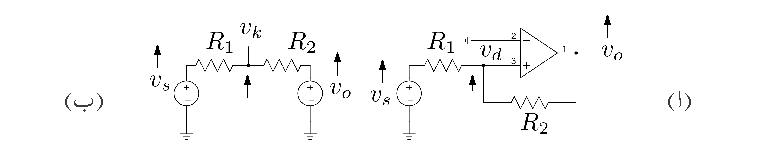
\includegraphics[scale=0.90]{feedbackPositiveOpampExplanation}
\caption{مثبت واپسی دور کی مثال}
\label{شکل_حسابی_مثبت_واپسی_دور}
\end{figure}
آئیں شکل \حوالہ{شکل_حسابی_مثبت_واپسی_دور} کو مثال بناتے ہوئے \اصطلاح{مثبت واپسی ادوار} حل کرنا دیکھتے ہیں۔تصور کریں کہ \عددی{v_s=0} اور \عددی{v_o=0} صفر ہیں۔یوں شکل  الف     میں 
\begin{align*}
v_k=\frac{R_2 v_s+R_1 v_o}{R_1+R_2}=0
\end{align*}
حاصل ہوتا ہے۔یوں \عددی{v_d=v_k-v_n} بھی صفر رہے گا۔جیسا کہ ہم اب دیکھیں گے کہ اس حال میں مثبت واپسی دور نہایت غیر مستحکم حال میں ہے۔تصور کریں کہ کسی وجہ سے \عددی{v_s} کی قیمت بڑھ کر \عددی{v_s=\Delta v} ہو جاتی ہے۔حسابی ایمپلیفائر کے رد عمل سے پہلے \عددی{v_o=0} ہی رہے گا اور یوں
\begin{align*}
v_k=\frac{R_2 \times \Delta v+R_1 \times  0}{R_1+R_2}=\left(\frac{R_2}{R_1+R_2}\right) \Delta v \\
v_d=v_k-v_n=\left(\frac{R_2}{R_1+R_2}\right) \Delta v 
\end{align*}
ہوں گے۔حسابی ایمپلیفائر \عددی{v_d} کو \عددی{A_d} گنا بڑھانا چاہے گا۔آئیں \عددی{v_o} کے بڑھنے کے عمل کو دیکھیں۔تصور کریں کہ خارجی اشارہ  بڑھتے بڑھتے \عددی{v_o=\Delta v_{o1}} ہو جاتا ہے۔اس طرح 
\begin{align*}
v_k=\frac{R_2 \times \Delta v+R_1 \times  \Delta v_{o1}}{R_1+R_2}=v_d
\end{align*}
ہو جائے گا۔جیسا کہ آپ دیکھ سکتے ہیں \عددی{v_d} کی قیمت پہلے سے بڑھ گئی ہے۔یوں \عددی{v_o} مزید بڑھے گا جس سے \عددی{v_d} مزید بڑھے گا۔آخر کار \عددی{v_o} مثبت منبع پر رکھ جائے گا یعنی \عددی{v_o=V_{CC}} ہو جائے گا۔اس وقت
\begin{align*}
v_k=\frac{R_2 \times \Delta v+R_1 \times  V_{CC}}{R_1+R_2} \approx \left(\frac{R_1}{R_1+R_2} \right) V_{CC}=v_d
\end{align*}
ہو گا۔آپ دیکھ سکتے ہیں کہ مثبت واپسی دور میں 
\begin{align}
v_k \ne v_n
\end{align}
ہوتے ہیں۔اسی وجہ سے \اصطلاح{مثبت ادوار} کو اس باب میں استعمال ہونے والے طریقے سے حل نہیں کیا جا سکتا جہاں ہم \عددی{v_k} اور \عددی{v_n} کے مساوات حاصل کرتے ہوئے  \عددی{v_k=v_n} تصور کر کے \عددی{v_o} کے لئے حل کرتے ہیں۔

\اصطلاح{مثبت واپسی دور} کی پہچان یہ ہے کہ اس کا خارجی اشارہ جب بھی حرکت کرے تو یہ اسی جانب حرکت کرتا ہے جس جانب دور کا داخلی اشارہ (بغیر واپس آئے) حرکت کرے۔

\ابتدا{مثال}
شکل \حوالہ{شکل_حسابی_مثبت_واپسی_دور} میں 
\begin{align*}
R_1=\SI{1}{\kilo \ohm} \hspace{5mm} R_2=\SI{9}{\kilo \ohm} \hspace{5mm} V_{CC}=\SI{12}{\volt} \hspace{5mm} V_{EE}=\SI{-12}{\volt}
\end{align*}
لیتے ہوئے \عددی{v_s} کی وہ قیمت حاصل کریں جس پر خارجی اشارہ مکمل منفی  سے مکمل مثبت جانب حرکت کرے گا۔ اسی طرح \عددی{v_s} کی وہ قیمت حاصل کریں جس پر خارجی اشارہ مکمل مثبت  سے مکمل منفی جانب حرکت کرے گا۔

حل:
تصور کریں کہ خارجی اشارہ مکمل منفی جانب ہے یعنی \عددی{v_o=\SI{-12}{\volt}} جبکہ \عددی{v_s=0} ہے۔اس وقت
\begin{align*}
v_k=v_d=\frac{9000 \times 0+1000 \times  12}{1000+9000}=\SI{1.2}{\volt}
\end{align*}
ہو گا۔\عددی{v_o} اس لمحہ منفی جانب حرکت کرے گا جب \عددی{v_d} کی قیمت منفی ہو جائے۔آئیں \عددی{v_d=0} پر درکار \عددی{v_s} کی قیمت حاصل کریں۔
\begin{align*}
0=\frac{9000 \times v_s+1000 \times  12}{1000+9000}\\
v_s=\SI{-1.333}{\volt}
\end{align*}
حاصل ہوتا ہے۔جوں ہی \عددی{v_s} کی قیمت \SI{-1.333}{\volt} سے کم ہو جائے، اسی لمحہ \عددی{v_o=\SI{-12}{\volt}} ہو جائے گا۔

اسی طرح اگر \عددی{v_o=\SI{-12}{\volt}} ہے  تو خارجی اشارہ اس وقت مثبت جانب حرکت کرے گا جب
\begin{align*}
0=\frac{9000 \times v_s+1000 \times  \left(-12\right)}{1000+9000}\\
v_s=\SI{1.333}{\volt}
\end{align*}
\عددی{v_s>\SI{1.333}{\volt}} ہو۔
\انتہا{مثال}
%================

شکل \حوالہ{شکل_حسابی_زنجیری} میں دو منفی حسابی ایمپلیفائر سلسلہ وار جوڑتے ہوئے زنجیری ایمپلیفائر حاصل کیا گیا ہے۔زنجیر کے پہلی کڑی کا داخلی اشارہ \عددی{v_{s1}} جبکہ اس کا خارجی اشارہ  \عددی{v_{o1}} اور اس کی افزائش \عددی{A_{v1}=-\tfrac{R_2}{R_1}} ہے۔زنجیر کے دوسری کڑی کا داخلی اشارہ  \عددی{v_{s2}} جبکہ اس کا خارجی اشارہ  \عددی{v_{o2}} اور اس کی افزائش \عددی{A_{v2}=-\tfrac{R_4}{R_3}} ہے۔پہلے کڑی کے خارجی اشارے کو دوسرے کڑی کو بطور داخلی اشارہ مہیا کیا گیا ہے لہٰذا \عددی{v_{s2}=v_{o1}} ہے۔یوں ہم لکھ سکتے ہیں۔
\begin{align*}
v_{o1}&=A_{v1} v_{s1}
\end{align*}
اور
\begin{align*}
v_{o2}&=A_{v2} v_{s2}\\
&=A_{v2} v_{o1}
\end{align*}
اس مساوات میں گزشتہ مساوات سے حاصل \عددی{v_{o1}} استعمال کرتے ہوئے
\begin{align*}
v_{o2}=A_{v2} A_{v1} v_{s1}
\end{align*}
لکھا جا سکتا ہے۔زنجیری ایمپلیفائر کا داخلی اشارہ \عددی{v_{s1}} جبکہ اس کا خارجی اشارہ \عددی{v_{o2}} ہے۔یوں زنجیری ایمپلیفائر کی افزائش \عددی{A_{v}=\tfrac{v_{o2}}{v_{s1}}} کو مندرجہ بالا مساوات سے یوں حاصل کر سکتے ہیں۔
\begin{align}
A_v=\frac{v_{o2}}{v_{s1}}=A_{v1} A_{v2}
\end{align}
یہ ایک اہم نتیجہ ہے جس کے مطابق ایمپلیفائر سلسلہ وار جوڑنے سے ان کی افزائش آپس میں ضرب ہوتی ہے۔زنجری ایمپلیفائر میں مزید کڑیاں اسی طرح سلسلہ وار جوڑی جا سکتی ہیں۔
\begin{figure}
\centering
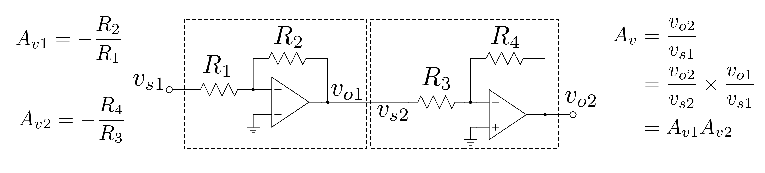
\includegraphics[scale=0.90]{cascadedOpampAmplifiers}
\caption{زنجیری حسابی ایمپلیفائر}
\label{شکل_حسابی_زنجیری}
\end{figure}

\جزوحصہ{مثبت ایمپلیفائر}

	شکل \حوالہ{شکل_مثبت_ایمپلیفائر}  میں ایک اور واپسی دور دکھایا گیا ہے جسے \اصطلاح{مثبت ایمپلیفائر}\فرہنگ{مثبت ایمپلیفائر}
\فرہنگ{amplifier!non-inverting}\حاشیہب{non-inverting amplifier}  کہتے ہیں۔آئیں اس دور کو کرخوف کے قوانین کی مدد سے حل کرتے ہیں۔
\begin{figure}
\centering
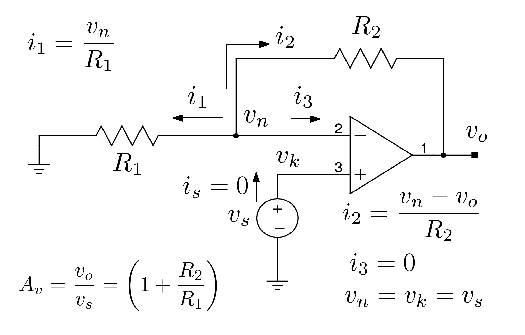
\includegraphics[scale=0.90]{nonInvertingAmplifier}
\caption{مثبت ایمپلیفائر}
\label{شکل_مثبت_ایمپلیفائر}
\end{figure}
	اس شکل میں جوڑ \عددی{v_n} سے باہر کی جانب تین برقی رو \عددیء{i_1}،\عددی{i_2} اور\عددی{i_3} نکلتے دکھائے گئے ہیں۔\عددی{i_3}چونکہ حسابی ایمپلیفائر کے داخلی سرے پر اندر کی جانب جاتی برقی رو ہے لہٰذا یہ مساوات \حوالہ{مساوات_حسابی_بنیادی_پہلو} کے شِق نمبر دو کی وجہ سے صفر کے برابر ہے۔باقی دو برقی رو کو اُوہم کے قانون کی مدد سے حاصل کیا جاتا ہے۔یوں
\begin{gather} 
\begin{aligned}\label{مساوات_مثبت_داخلی_سرے_پر_رو}
i_1 &=\frac{v_n}{R_1}\\
i_2&=\frac{v_n-v_o}{R_2}\\
i_3&=0
\end{aligned}
\end{gather}
جوڑ \عددی{v_k} چونکہ سیدھا فراہم کردہ برقی اشارہ \عددی{v_s} کے ساتھ جڑا ہے لہٰذا اس کے لئے ہم لکھ سکتے ہیں
\begin{align} \label{مساوات_مثبت_داخلی_دباو_اشارے_کے_برابر}
v_k = v_s
\end{align}
	کرخوف کے قانون برائے برقی رو کو مساوات \حوالہ{مساوات_مثبت_داخلی_سرے_پر_رو}  کے ساتھ مل کر استعمال کرتے حاصل ہوتا ہے
\begin{align} \label{مساوات_مثبت_افزائش_کا_حصول}
&i_1+i_2+i_3=0 \nonumber\\
&\frac{v_n}{R_1}+\frac{v_n-v_o}{R_2}+0=0
\end{align}
مساوات \حوالہ{مساوات_حسابی_بنیادی_پہلو} کی پہلی شق کے مطابق \عددی{v_k}  اور \عددی{v_n} کی قیمتیں برابر رہتی ہیں۔یوں مساوات \حوالہ{مساوات_مثبت_داخلی_دباو_اشارے_کے_برابر}  میں دیے \عددی{v_k} کی قیمت کو مساوات \حوالہ{مساوات_مثبت_افزائش_کا_حصول}  میں \عددی{v_n} کی جگہ استعمال کرتے ہم مساوات \حوالہ{مساوات_مثبت_افزائش_کا_حصول}  کو حل کرتے ہیں۔
\begin{align}
\frac{v_s}{R_1}+\frac{v_s-v_o}{R_2} &=0 \nonumber \\
\frac{v_s}{R_1}+\frac{v_s}{R_2}-\frac{v_o}{R_2}&=0 \nonumber \\
\left (  \frac{v_s}{R_1} +\frac{v_s}{R_2}\right ) R_2 &=v_o \nonumber \\
\left(1+\frac{R_2}{R_1} \right )v_s &=v_o
\end{align}
اس مساوات کو عموماً یوں لکھا جاتا ہے۔
\begin{align} \label{مساوات_مثبت_افزائش}
A_v=\frac{v_o}{v_s}=\left(1+\frac{R_2}{R_1} \right )
\end{align}
\عددی{v_o} اور \عددی{v_s} کے کسر کو \اصطلاح{مثبت ایمپلیفائر} کی \اصطلاح{برقی دباو کی افزائش}\فرہنگ{افزائش!برقی دباو}\حاشیہب{voltage gain}\فرہنگ{voltage gain} \عددی{A_v} کہتے ہیں۔اس اصطلاح کو عموماً چھوٹا کر کے اسے صرف \اصطلاح{مثبت افزائش} کہتے ہیں۔

اس ایمپلیفائر کا داخلی مزاحمت حاصل کرنے کی خاطر \عددی{v_s} لاگو کرتے ہوئے \عددی{i_s} ناپتے ہیں۔چونکہ حسابی ایمپلیفائر کا داخلی برقی رو صفر ہوتا ہے لہٰذا \عددی{i_s=0} ہو گا۔یوں 
\begin{align}
R_{\textup{داخلی}}=\frac{v_s}{i_s}=\frac{v_s}{0} \to \infty
\end{align}
حاصل ہوتا ہے۔
%==============
\ابتدا{مثال}
شکل \حوالہ{شکل_مثبت_ایمپلیفائر} میں دکھلائے مثبت ایمپلیفائر میں \عددی{R_1 = \SI{2}{\kilo \ohm}} اور \mbox{\عددی{R_2=\SI{15}{\kilo \ohm}}} تصور کریں۔اس مثبت ایمپلیفائر کو باری باری مندرجہ ذیل برقی اشارات بطور \عددی{v_s} مہیا کیا جاتا ہے۔ان تمام کے لئے حسابی دور کا خارجی اشارہ \عددی{v_o} حاصل کریں۔حل کرتے وقت \عددی{V_{CC}=\SI{+15}{\volt}}  اور  \عددی{V_{EE}=\SI{-15}{\volt}} تصور کریں۔
\begin{enumerate}
\item 
$ \begin{aligned}
v_s = \SI{1.2}{\volt}
\end{aligned} $

\item 
$ \begin{aligned}
v_s = \SI{-0.25}{\volt}
\end{aligned} $

\item 
$ \begin{aligned}
v_s = 0.33 \cos (\omega t)
\end{aligned} $
\end{enumerate}
حل:	مساوات  \حوالہ{مساوات_مثبت_افزائش} سے اس مثبت ایمپلیفائر کی افزائش حاصل کرتے ہیں۔
\begin{align*}
A_v = \left (1+\frac{15000}{2000} \right )=\SI{8.5}{\volt \per \volt}
\end{align*}
یوں
\begin{enumerate}
\item
$\begin{aligned}
v_o=A_v \times v_s = 8.5 \times 1.2=\SI{10.2}{\volt}
\end{aligned}$

\item
$\begin{aligned}
v_o=A_v \times v_s = 8.5 \times (-0.25)=\SI{2.125}{\volt}
\end{aligned}$

\item
$\begin{aligned}
v_o=A_v \times v_s = 8.5 \times 0.33 \cos (\omega t)=2.805 \cos (\omega t)
\end{aligned}$
\end{enumerate}
\انتہا{مثال}

%============

	اس مثال میں داخلی اشارہ مثبت ہونے کی صورت میں خارجی اشارہ  مثبت ہے جبکہ داخلی اشارہ منفی ہونے کی صورت میں خارجی اشارہ بھی منفی ہے۔یوں مثبت ایمپلیفائر داخلی اشارہ کو بغیر الٹائے بڑھا کر خارج کرتا ہے۔اسی لئے اسے \اصطلاح{مثبت ایمپلیفائر}\فرہنگ{مثبت ایمپلیفائر}\فرہنگ{amplifier!non-inverting}\حاشیہب{non-inverting amplifier}  کہتے ہیں۔

\جزوحصہ{مستحکم کار}

	مثبت ایمپلیفائر کی افزائش یہاں دوبارہ پیش کرتے ہیں۔
\begin{align}
A_v=1+\frac{R_2}{R_1}
\end{align}
اگر مثبت ایمپلیفائر میں \عددی{R_1} کی قیمت لامحدود لی جائے اور \عددی{R_2} کی قیمت صفر اُوہم  لی جائے تو اس مساوات کے مطابق اس کی افزائش
\begin{align}
A_v=1+\frac{0}{\infty} =1
\end{align}
ہو گی۔ایسا دور جسے \اصطلاح{مستحکم کار}\فرہنگ{مستحکم کار}\فرہنگ{buffer}\حاشیہب{buffer}  کہتے ہیں کو شکل \حوالہ{شکل_وسطی_دور} میں دکھایا گیا ہے۔اس دور کی افزائش ایک کے برابر جبکہ داخلی مزاحمت لامحدود ہے۔
\begin{figure}
\centering
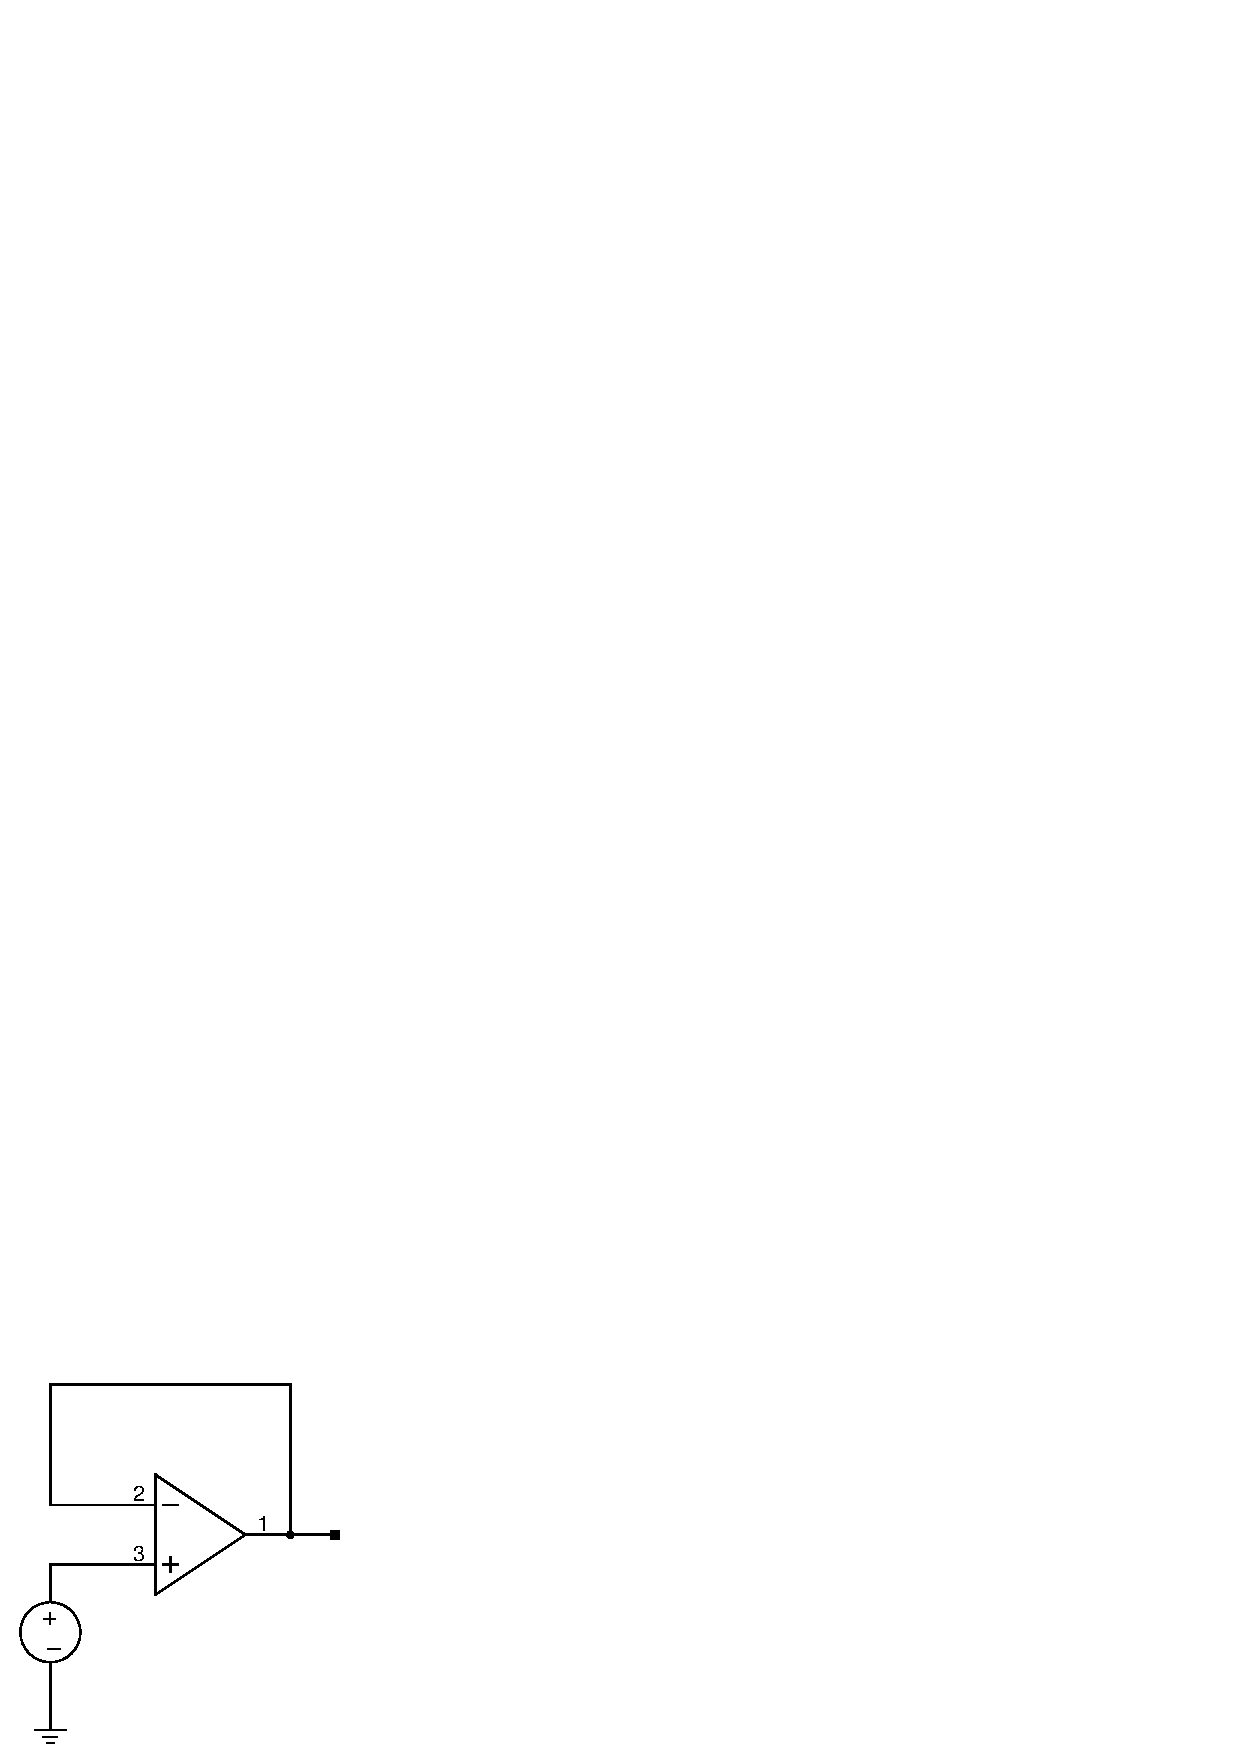
\includegraphics[scale=0.90]{opampBuffer}
\caption{مستحکم کار}
\label{شکل_وسطی_دور}
\end{figure}
اس دور کو یوں بھی سمجھا جا سکتا ہے کہ مثبت داخلی سرے پر برقی دباو \عددی{v_s} ہے۔یوں منفی داخلی سرے پر  بھی اتنا ہی برقی دباو ہو گا مگر یہ سرا اور خارجی سرا آپس میں جڑے ہیں۔یوں خارجی سرے پر بھی یہی برقی دباو ہو گا یعنی \عددی{v_o = v_s} ہو گا جس سے افزائش \عددی{\tfrac{v_o}{v_s}=1} حاصل ہوتی ہے۔آئیں \اصطلاح{مستحکم کار} کا استعمال جانیں۔ 

طبعی متغیرات\حاشیہب{variables} مثلاً  کمیت، حرارت وغیرہ  کی برقیاتی پیمائش سے پہلے انہیں عموماً  \اصطلاح{مبدل توانائی}\فرہنگ{مبدل توانائی}\فرہنگ{transducer}\حاشیہب{transducer}  کے مدد سے برقی اشارات میں تبدیل کیا جاتا ہے اور ان برقی اشارات کو پیمایشی آلہ\فرہنگ{پیمایشی آلہ}\حاشیہب{measuring instrument}  سے ناپا جاتا ہے۔

	جیسا کہ آپ جانتے ہیں کہ کسی بھی دور کا \اصطلاح{تھونن  مساوی} دور\فرہنگ{تھونن دور}\حاشیہب{Thevenin circuit} بنایا جا سکتا ہے جسے ایک عدد منبع برقی دباو اور ایک عدد مزاحمت کی شکل دی جاتی ہے۔مبدل توانائی کا تھونن دور شکل \حوالہ{شکل_وسطی_دور_حساس_اشارہ} الف میں بائیں جانب نقطہ دار لکیر میں گھیرا دکھایا گیا ہے جہاں \عددی{v_s} اس کی تھونن برقی دباو اور \عددی{R_S}  اس کی تھونن مزاحمت ہے۔پیمایشی آلہ داخلی سروں پر کسی قسم کا برقی اشارہ خارج نہیں کرتا بلکہ ان سروں پر یہ صرف اشارہ حاصل کرنے کی صلاحیت رکھتا ہے لہٰذا اس کے داخلی جانب کا تھونن دور صرف ایک عدد مزاحمت \عددی{R_M}  پر مبنی ہوتا ہے جیسے شکل-الف میں دائیں جانب دکھایا گیا ہے۔شکل-الف میں مبدل توانائی کے خارجی سروں کو پیمایشی آلہ کے داخلی سروں کے ساتھ جوڑا گیا ہے تا کہ مبدل توانائی کا اشارہ \عددی{v_s} ناپا جا سکے۔پیمایشی آلہ داخلی سروں  پر لاگو برقی دباو \عددی{v_m} ناپتا ہے۔
\begin{figure}
\centering
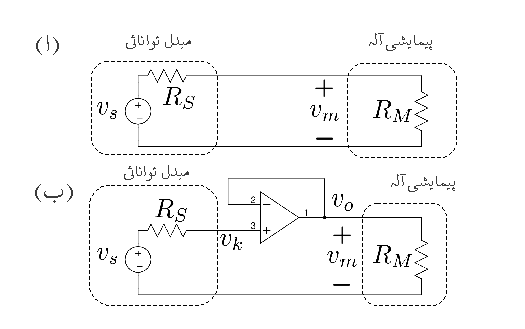
\includegraphics[scale=0.90]{bufferingWeakSignal}
\caption{مستحکم کار کی مدد سے حساس اشارہ کی  پیمائش}
\label{شکل_وسطی_دور_حساس_اشارہ}
\end{figure}
شکل-الف میں پیمایشی آلہ کے داخلی سروں پر
\begin{align*}
v_m=\left(\frac{R_M }{R_M+R_S} \right) v_s
\end{align*}
پایا جاتا ہے جسے پیمائشی آلہ پڑھے گا  اگرچہ حقیقت میں اشارہ کی اصل قیمت \عددی{v_s}  ہے۔

	مثال کے طور پر اگر \عددیء{R_S=\SI{5}{\mega \ohm}}،\عددی{R_M=\SI{10}{\mega \ohm}} اور اشارہ کی قیمت \عددی{v_s = \SI{100}{\milli \volt}}ہو تب پیمائشی آلہ
\begin{align*}
v_m = \frac{10 \times 10^{6} \times 100 \times 10^{-3}}{10 \times 10^{6}+5 \times 10^{6}}=\SI{66.66}{\milli \volt}
\end{align*}
پڑھے گا۔آپ دیکھ سکتے ہیں کہ یہ نا قابل قبول صورت حال ہے۔

مبدل توانائی تخلیق دیتے وقت کوشش کی جاتی ہے کہ اس کے تھونن مساوی مزاحمت \عددی{R_S} کی قیمت کم سے کم ہو۔اسی طرح پیمایشی آلہ تخلیق دیتے وقت کوشش کی جاتی ہے کہ اس کے داخل مزاحمت \عددی{R_M} کی قیمت زیادہ سے زیادہ ہو۔یوں آپ دیکھ سکتے ہیں کہ اگر \عددی{R_M \gg R_S} ہو تب \عددی{v_m \approx v_s} ہو گا۔

آپ دیکھ سکتے ہیں کہ پیمایشی آلے کی داخلی مزاحمت مبدل توانائی پر بوجھ ڈالتی ہے جس سے مبدل کے بیرونی سروں پر میسر اشارے کی قیمت میں کمی رونما ہوتی ہے۔یوں بوجھ کو ہلکا کرنے کی خاطر \عددی{R_M} کی قیمت بڑھانی ہو گی۔اس مثال میں مبدل توانائی کو پیمایشی آلہ بطور \اصطلاح{برقی بوجھ} \حاشیہب{load}  نظر آتا ہے۔یہ بوجھ جتنا کم ہو اتنا بہتر ہو گا۔

اس مسئلے کو \اصطلاح{مستحکم کار} کی مدد سے با آسانی حل کیا جا سکتا ہے۔شکل \حوالہ{شکل_وسطی_دور_حساس_اشارہ} ب میں مبدل توانائی اور پیمایشی آلہ کے وسط میں \اصطلاح{مستحکم کار} نسب کیا گیا ہے۔چونکہ حسابی ایمپلیفائر کا داخلی مزاحمت لامحدود ہوتا ہے اور اس کی داخلی برقی رو صفر ہوتی ہے لہٰذا اس دور میں مزاحمت \عددی{R_S} میں اُوہم کے قانون کے تحت صفر برقی دباو گھٹے گا اور یوں \عددی{v_k = v_s}  اور \عددی{v_o = v_s}  ہو گا۔چونکہ مزاحمت \عددی{ R_M} کو یہی برقی دباو فراہم کیا جاتا ہے لہٰذا \عددی{v_m = v_o = v_s} ہو گا۔


\اصطلاح{مستحکم کار} کا کمال یہ ہے کہ یہ برقی بوجھ \عددی{R_M} کو ازخود اٹھا لیتا ہے اور اس کا بوجھ مبدل توانائی پر نہیں ڈالتا۔یوں یہ حساس اشارات کو مستحکم کرتا ہے۔

آپ نے دیکھا کہ \اصطلاح{مستحکم کار} کی مدد سے اشارہ کی صحیح قیمت حاصل ہوتی ہے۔ حساس اور باریک اشارات کی پیمائش عموماً مستحکم کار کے مدد سے ہی کی جاتی ہے۔

\جزوجزوحصہ{بدلتا رو مستحکم کار}
عموماً اشارے کے یک سمت حصے کو روکتے ہوئے اس کے بدلتے حصے کو مستحکم بنانے کی ضرورت ہوتی ہے۔ایسی صورت میں \اصطلاح{بدلتا رو مستحکم کار} جسے شکل \حوالہ{شکل_بدلتا_رو_وسطی_دور} میں دکھایا گیا ہے استعمال کیا جائے گا۔\عددی{C_1} اور \عددی{C_2} کی قیمت اتنی رکھی جاتی ہے کہ درکار تعدد پر انہیں قصر دور تصور کیا جا سکے۔مزاحمت \عددی{R_1} اور \عددی{R_2} حسابی ایمپلیفائر کے مثبت داخلی سرے  کے \اصطلاح{داخلی میلان برقی رو}\حاشیہد{داخلی میلان برقی پر حصہ \حوالہ{حصہ_حسابی_داخلی_برقی_رو} میں غور کیا جائے گا۔} کے لئے راستہ فراہم کرتے ہیں۔\عددی{C_1} داخلی اشارے کے بدلتے جزو کو حسابی ایمپلیفائر کے مثبت داخلی سرے  تک پہنچنے کا راستہ فراہم کرتے ہوئے یک سمت جزو کو روکتا ہے۔\عددی{C_2} کے عدم موجودگی میں داخلی اشارے کو بدلتا داخلی مزاحمت \عددی{R_1+R_2} نظر آتا جبکہ مستحکم کار سے توقع کی جاتی ہے کہ اس کا داخلی مزاحمت بہت زیادہ ہو۔آئیں دیکھیں کہ \عددی{C_2} کی شمولیت سے داخلی مزاحمت کیسے بڑھتی ہے۔
\begin{figure}
\centering

\includegraphics[scale=0.90]{bootstrapOpampBased}
\caption{بدلتا رو مستحکم کار}
\label{شکل_بدلتا_رو_وسطی_دور}
\end{figure}
\عددی{v_S} کا بدلتا جزو \عددی{v_s} مثبت داخلی سرے پر پہنچتا ہے۔یوں \عددی{v_n=v_s} ہو گا جس سے \عددی{v_n=v_k=v_s} اور \عددی{v_o=v_s} ہو گا۔\عددی{C_2} درکار  تعدد پر قصر دور ہو گا اور یوں \عددی{R_1} اور \عددی{R_2} کے جوڑ پر بھی \عددی{v_s} اشارہ پایا جائے گا۔اب دوبارہ داخلی جانب سے سوچیں۔حسابی ایمپلیفائر کا مثبت داخلی سرا  از خود کوئی برقی رو گزرنے نہیں دیتا۔چونکہ مزاحمت \عددی{R_1} کے دونوں سروں پر \عددی{v_s} برقی دباو پایا جاتا ہے لہٰذا اس میں گزرتی برقی رو بھی صفر ہے۔یوں \عددی{v_s} سے کسی قسم کا برقی رو حاصل نہیں کیا جاتا جو کہ منقطع صورت کی نشانی ہے۔یوں بدلتا مستحکم کار درکار تعدد پر لامحدود داخلی مزاحمت پیش کرتے ہوئے حساس اشارے پر بالکل بوجھ نہیں ڈالتا۔

کسی بھی ایمپلیفائر جس کی  \عددی{A_v \approx 1} ہو،  کے  خارجی سرے  سے داخلی جانب یوں کپیسٹر  نسب کر کے اس کا داخلی مزاحمت بڑھایا جا سکتا ہے۔شرط صرف یہ ہے کہ درکار تعدد پر کپیسٹر قصر دور کام کرتے ہوئے مکمل خارجی اشارے کو داخلی جانب مزاحمت \عددی{R_1} تک  پہنچا سکے۔مزاحمت \عددی{R_1} کے ایک سرے کو جس جانب  داخلی اشارہ کھینچتا ہے، خارجی اشارہ بھی اسی جانب مزاحمت کا دوسرا سرا کھینچتا ہے۔

\جزوحصہ{تفرق کار}
ایک اور اہم دور جسے \اصطلاح{تفرق کار}\فرہنگ{تفرق کار}\فرہنگ{differentiator}\حاشیہب{differentiator}  کہتے ہیں کو شکل \حوالہ{شکل_تفرق_کار} میں دکھایا گیا ہے۔
\begin{figure}
\centering
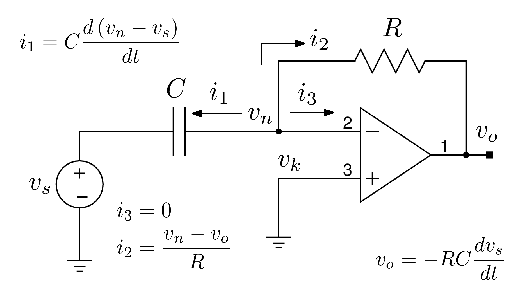
\includegraphics[scale=0.90]{differentiator}
\caption{تفرق کار}
\label{شکل_تفرق_کار}
\end{figure}
	اس دور کو بالکل پہلی دو ادوار کی طرح حل کرتے ہیں۔جوڑ پر تین برقی رو کے لئے لکھ سکتے ہیں۔
\begin{align} \label{مساوات_تفرق_کار_کے_مساوات_کا_حصول}
i_1 &= C \od{\left (v_n-v_s \right )}{t} \nonumber \\
i_2 &=\frac{v_n-v_o}{R} \nonumber \\
i_3 &=0
\end{align}
جبکہ جوڑ \عددی{v_k} کے لئے لکھ سکتے ہیں۔
\begin{align}
v_k=0
\end{align}
کرخوف کے قانون برائے برقی رو کو جوڑ \عددی{v_n} پر یوں لکھا جا سکتا ہے۔
\begin{align} \label{مساوات_تفرق_کار_داخلی_جوڑ_پر_رو}
i_1+i_2+i_3=0
\end{align}
مساوات \حوالہ{مساوات_تفرق_کار_کے_مساوات_کا_حصول} میں دیے گئے قیمتوں کو مساوات \حوالہ{مساوات_تفرق_کار_داخلی_جوڑ_پر_رو}  میں پر کرتے ہیں
\begin{align*}
C \od{\left(v_n-v_s\right)}{t}+\frac{v_n-v_o}{R}+0&=0
\end{align*}
\عددی{v_n=v_k} لیتے ہوئے  \عددی{v_n=0} کرتے ہوئے
\begin{align*}
 -C \od{v_s}{t}-\frac{v_o}{R}&=0
\end{align*}
حاصل ہوتا ہے جسے یوں لکھ سکتے ہیں۔
\begin{align}
v_o = -RC \od{v_s}{t}
\end{align}
اس مساوات کے تحت یہ دور مہیا کردہ اشارہ \عددی{v_s} کے تفرق کے نسبت سے خارجی اشارہ \عددی{v_o} پیدا کرتا ہے۔اسی سے اس دور کو \اصطلاح{تفرق کار}\حاشیہب{differentiator}  کہتے ہیں۔


\جزوحصہ{تکمل کار}

تفرقی دور کو دیکھنے کے بعد خیال آتا ہے کہ کیا حسابی ایمپلیفائر کو استعمال کرتے کسی تفاعل کا \اصطلاح{تکمل}\حاشیہب{integral} حاصل کیا جا سکتا ہے۔جواب ہے جی ہاں۔\اصطلاح{تکمل کار}\فرہنگ{تکمل کار}\فرہنگ{integrator}\حاشیہب{integrator}  کو شکل \حوالہ{شکل_تکمل_کار}  میں دکھایا گیا ہے۔
\begin{figure}
\centering
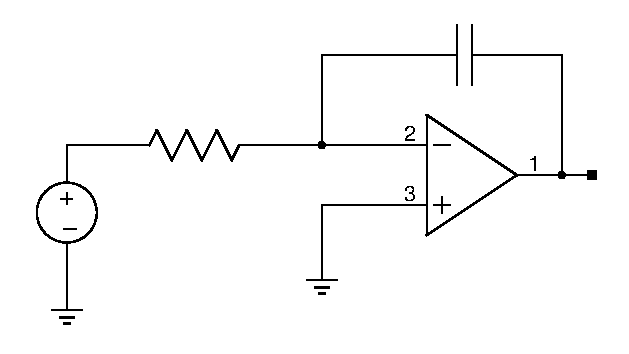
\includegraphics[scale=0.90]{integrator}
\caption{تکمل کار}
\label{شکل_تکمل_کار}
\end{figure}
اس دور کے لئے ہم لکھ سکتے ہیں
\begin{gather}
\begin{aligned}
i_1 & = \frac{v_n-v_s}{R} \\
i_2 &= C \od{ (v_n-v_o )}{t} \\
i_3&=0
\end{aligned}
\end{gather}
اور
\begin{align}
v_k =0
\end{align}
کرخوف کا قانون برائے برقی رو استعمال کرتے ہوئے اور \عددی{v_n}  میں \عددی{v_k} کی قیمت (یعنی صفر وولٹ) استعمال کرتے ہوئے حل کرتے ہیں۔
\begin{align*}
i_1+i_2+i_3&=0  \\
\frac{v_n-v_s}{R}+C \od{(v_n-v_o)}{t}+0&=0\\
-\frac{v_s}{R}-C\od{v_o}{t}&=0
\end{align*}
اس کا تکملہ لیتے ہیں
\begin{align*}
\od{v_o}{t}&=-\frac{v_s}{RC}\\
\mathrm{d}v_o&=-\frac{v_s}{RC} \, \mathrm{d}t\\
\int {\mathrm{d}v_o} & =-\int \frac{v_s}{RC} \, \mathrm{d}t
\end{align*}
یعنی
\begin{align} \label{مساوات_حسابی_تکمل_کار}
v_o&=-\frac{1}{RC} \int v_s \, \mathrm{d}t 
\end{align}
اس مساوات میں \عددی{v_o} حاصل کرنے کی خاطر مساوات کے نشان کے دونوں جانب کا تکملہ لیا گیا ہے۔اس طرح تکمل کار کا خارجی اشارہ  \عددی{v_o} اسے مہیا کئے گئے اشارہ\عددی{v_s}کے تکملہ کے براہِ راست متناسب ہوتا ہے۔اسی خاصیت کی وجہ سے اس دور کو \قریب{\اصطلاح{تکمل کار}}\فرہنگ{تکمل کار}\فرہنگ{integrator}\حاشیہب{integrator}  کہتے ہیں۔

%=================
\ابتدا{مثال}
\عددی{R=\SI{1}{\kilo \ohm}} اور \عددی{C=\SI{6.8}{\micro \farad}} اور \عددی{v_s=V_p \sin \omega t} کی صورت میں
\begin{itemize}
\item
 \اصطلاح{تکمل کار}  کا خارجی اشارہ حاصل کریں۔
\item
کتنی تعدد پر خارجی اشارے کا حیطہ داخلی اشارے کے حیطے  کے برابر ہو گا۔
\item
خارجی اور داخلی اشارے کا زاویاتی تعلق کیا ہے۔
\end{itemize}
حل:
\begin{itemize}
\item
مساوات \حوالہ{مساوات_حسابی_تکمل_کار} کی مدد سے
\begin{align*}
v_o=-\frac{1}{1000 \times 6.8 \times 10^{-6}} \int V_p \sin \omega t \, \mathrm{d} t=\frac{147 V_p}{\omega} \cos \omega t
\end{align*}
حاصل ہوتا ہے۔
\item
دونوں حیطے برابر اس وقت ہوں گے جب
\begin{align*}
\frac{147 V_p}{\omega}=V_p\\
\omega = 147\\
f=\frac{147}{2 \pi} =\SI{23.396}{\hertz}
\end{align*}
ہو گا۔
\item
داخلی اشارے کو یوں لکھتے ہوئے
\begin{align*}
v_s=V_p \sin \omega t= V_p \cos \left(\omega t-\SI{90}{\degree}\right)
\end{align*}
ہم دیکھتے ہیں کہ داخلی اشارے سے خارجی اشارہ \عددی{\SI{90}{\degree}} \اصطلاح{آگے}\حاشیہب{leading} ہے۔
\end{itemize}
\انتہا{مثال}
%==============
\ابتدا{مثال}
\عددی{R=\SI{1}{\kilo \ohm}} اور \عددی{C=\SI{10}{\micro \farad}} اور \عددی{v_s=\SI{-0.1}{\volt}} کی صورت میں \عددی{v_o} حاصل کریں۔

حل:
\begin{align*}
v_o=-\frac{1}{1000 \times 10 \times 10^{-6}} \int -0.1 \, \mathrm{d}t =10 t
\end{align*}
حاصل ہوتا ہے۔آپ دیکھ سکتے ہیں کہ خارجی اشارہ وقت کے راست تناسب بڑھتا ہے۔یہ ایک سیکنڈ میں دس وولٹ بڑھ رہا ہے۔اگر داخلی اشارہ مثبت کر دیا جائے تو خارجی اشارہ منفی جانب رواں ہو جائے گا۔
\انتہا{مثال}

شکل \حوالہ{شکل_تکمل_کار_مثال} میں دو مختلف داخلی اشارات پر تکمل کار کا رد عمل دکھایا گیا ہے۔آپ یہاں رک کر تسلی کر لیں کہ خارجی اشارات آپ کے توقع کے عین مطابق ہیں۔
\begin{figure}
\centering
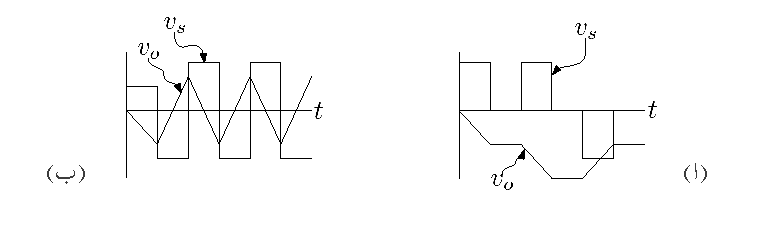
\includegraphics[scale=0.90]{integratorSquareWave}
\caption{تکمل کار کی کارکردگی کے مثال}
\label{شکل_تکمل_کار_مثال}
\end{figure}

%=========================
\جزوحصہ{جمع کار}

حسابی ایمپلیفائر کو دو یا دو سے زیادہ اشارات کا مجموعہ حاصل کرنے کے لئے بھی استعمال کیا جا سکتا ہے۔ایسے ہی \اصطلاح{جمع کار}\فرہنگ{جمع کار}\فرہنگ{adder}\حاشیہب{adder}  کو شکل \حوالہ{شکل_جمع_کار} میں دکھایا گیا ہے۔
\begin{figure}
\centering
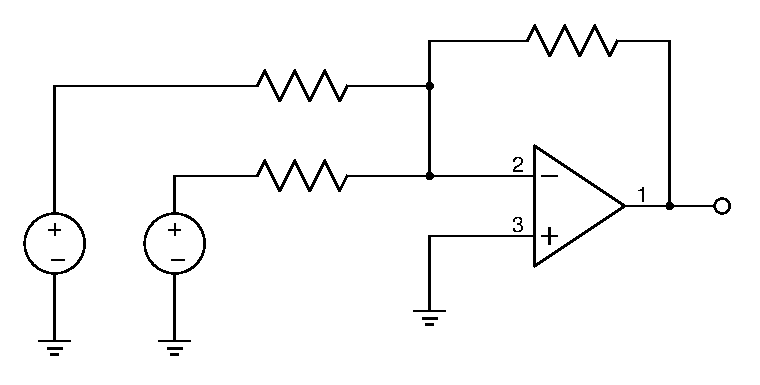
\includegraphics[scale=0.90]{adder}
\caption{جمع کار}
\label{شکل_جمع_کار}
\end{figure}
	اس شکل میں دو اشارات \عددی{v_{s1}} اور \عددی{v_{s2}} مہیا کئے گئے ہیں۔اشارہ \عددی{v_{s1}} مزاحمت \عددی{R_1} کے ذریعہ حسابی ایمپلیفائر کے \عددی{v_n} سرے کے ساتھ جڑا ہے۔اسی طرح اشارہ \عددی{v_{s2}} مزاحمت \عددی{R_2} کے ذریعہ حسابی ایمپلیفائر کے \عددی{v_n} سرے کے ساتھ جڑا ہے۔مزید اشارات کو بھی اسی ترکیب سے جوڑا جا سکتا ہے۔شکل میں دکھائی گئی برقی رو کے لئے یوں لکھ سکتے ہیں۔
\begin{gather}
\begin{aligned}
i_1 &=\frac{v_n-v_{s1}}{R_1} \\
i_2 &=\frac{v_n-v_{s2}}{R_2} \\
i_3&=0 \\
i_o &=\frac{v_n-v_o}{R_0}
\end{aligned}
\end{gather}
اسی طرح جوڑ \عددی{v_k} کے لئے لکھ سکتے ہیں
\begin{align}
v_k =0
\end{align}
جوڑ \عددی{v_n} پر کرخوف کے قانون برائے برقی رو استعمال کرتے ہوئے حل کرتے ہیں۔
\begin{align*}
i_1+i_2+i_3+i_4&=0 \\
\frac{v_n-v_{s1}}{R_1}+\frac{v_n-v_{s2}}{R_2}+0+\frac{v_n-v_o}{R_0}&=0
\end{align*}
\عددی{v_n=v_k} لیتے ہوئے \عددی{v_n=0} پر کرتے ہوئے
\begin{align*}
-\frac{v_{s1}}{R_1}-\frac{v_{s2}}{R_2}-\frac{v_o}{R_0}=0
\end{align*}
حاصل ہوتا ہے جسے
\begin{align}
v_o= -R_0 \left (\frac{v_{s1}}{R_1}+\frac{v_{s2}}{R_2}  \right)
\end{align}
لکھ سکتے ہیں۔\عددیء{R_0}، \عددی{R_1}اور \عددی{R_2} کی قیمتیں برابر ہونے کی صورت میں اس مساوات کو یوں لکھ سکتے ہیں
\begin{align}
v_o = -R \left (\frac{v_{s1}}{R} +\frac{v_{s2}}{R}\right)=- \left (v_{s1}+v_{s2} \right )
\end{align}
اس صورت میں آپ دیکھ سکتے ہیں کہ منفی علامت کے علاوہ، \عددی{v_o}  دونوں اشارات کا مجموعہ ہے۔اسی لئے اس دور کو \اصطلاح{جمع کار}\فرہنگ{جمع کار}\فرہنگ{adder}\حاشیہب{adder}  کہتے ہیں۔


\جزوحصہ{منفی کار}

حسابی ایمپلیفائر سے دو اشارات منفی کرنے والے دور پر اس حصہ میں غور کرتے ہیں۔ اس دور کو شکل \حوالہ{شکل_منفی_کار} میں دکھایا گیا ہے۔
\begin{figure}
\centering
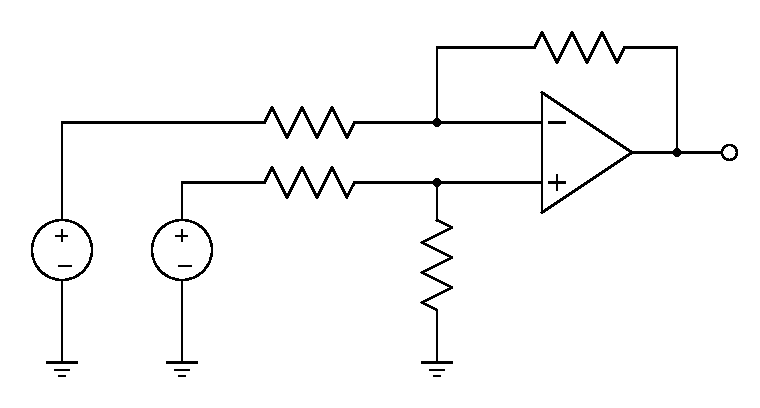
\includegraphics[scale=0.90]{subtractor}
\caption{منفی کار}
\label{شکل_منفی_کار}
\end{figure}
شکل کو دیکھتے ہم لکھ سکتے ہیں۔
\begin{gather}
\begin{aligned}
i_1 &= \frac{v_n-v_{s1}}{R_1}\\
i_2&=\frac{v_n-v_o}{R_2}\\
i_3&=\frac{v_k-v_{s2}}{R_3}\\
i_4&=\frac{v_k}{R_4}\\
i_5&=0\\
i_6&=0
\end{aligned}
\end{gather}
انہیں کرخوف کے قانون برائے برقی رو میں  استعمال کرتے ہوئے، جوڑ \عددی{v_n}  کے لئے یوں لکھ سکتے ہیں۔
\begin{gather} \label{مساوات_منفی_کار_منفی_سرے_پر_دباو}
\begin{aligned}
 i_1+i_2+i_5=0\\
\frac{v_n-v_{s1}}{R_1}+\frac{v_n-v_o}{R_2}+0=0\\
v_n \left(\frac{1}{R_1}+\frac{1}{R_2} \right)=\frac{v_{s1}}{R_1}+\frac{v_o}{R_2}\\
v_n=\frac{\frac{v_{s1}}{R_1}+\frac{v_o}{R_2}}{\frac{1}{R_1}+\frac{1}{R_2}}
\end{aligned}
\end{gather}
اسی طرح جوڑ \عددی{v_k}  پر کرخوف کا قانون برائے برقی رو لاگو کرتے ہوئے اسے یوں حل کر سکتے ہیں۔
\begin{gather} \label{مساوات_منفی_کار_مثبت_سرے_پر_دباو}
\begin{aligned}
i_3+i_4+i_6=0\\
\frac{v_k-v_{s2}}{R_3}+\frac{v_k}{R_4}+0=0\\
v_k \left(\frac{1}{R_3}+\frac{1}{R_4} \right)=\frac{v_{s2}}{R_3}\\
v_k=\frac{\frac{v_{s2}}{R_3}}{\frac{1}{R_3}+\frac{1}{R_4} }
\end{aligned}
\end{gather}
مساوات \حوالہ{مساوات_حسابی_بنیادی_پہلو} کی پہلی شق کے تحت \عددی{v_k}  اور \عددی{v_n} برابر ہوتے ہیں۔یوں مساوات \حوالہ{مساوات_منفی_کار_منفی_سرے_پر_دباو}  اور \حوالہ{مساوات_منفی_کار_مثبت_سرے_پر_دباو}  کو برابر ڈالتے ہوئے
\begin{align*}
v_n=v_k\\
\frac{\frac{v_{s1}}{R_1}+\frac{v_o}{R_2}}{\frac{1}{R_1}+\frac{1}{R_2}}=\frac{\frac{v_{s2}}{R_3}}{\frac{1}{R_3}+\frac{1}{R_4} }
\end{align*}
یعنی
\begin{gather}
\begin{aligned} \label{مساوات_حسابی_منفی_کار}
v_o&=\frac{R_4}{R_1} \left(\frac{R_1+R_2}{R_3+R_4} \right) v_{s2}-\frac{R_2}{R_1}v_{s1}\\
&=\left(\frac{1+\frac{R_2}{R_1}}{1+\frac{R_3}{R_4}} \right) v_{s2}-\frac{R_2}{R_1}v_{s1}
\end{aligned}
\end{gather}
حاصل ہوتا ہے۔یہ دور کی عمومی مساوات ہے۔اگر دور میں \عددی{R_1=R_3=R_a} جبکہ \عددی{R_2=R_4=R_b} ہوں تب اس مساوات سے
\begin{align}
v_o=\frac{R_b}{R_a}\left(v_{s2}-v_{s1}\right)
\end{align}
حاصل ہوتا ہے۔اگر \عددی{R_a}  اور\عددی{R_b} کی قیمتیں برابر ہوں تو اس صورت میں دور دونوں اشارات کو منفی کرے گا۔اسی لئے اس دور کو \اصطلاح{منفی کار}\فرہنگ{منفی کار}\فرہنگ{subtractor}\حاشیہب{subtractor} کہتے ہیں۔اگر\عددی{R_a} اور \عددی{R_b}برابر نہ ہوں تو دور دونوں اشارات میں فرق کو بڑھانے یا گھٹانے کی صلاحیت بھی رکھتا ہے

\ابتدا{مثال}
منفی کار کا مشترکہ داخلی مزاحمت تمام مزاحمت برابر ہونے کی صورت میں حاصل کریں۔تمام مزاحمت مختلف ہونے کی صورت میں جواب کیا ہو گا۔

\begin{figure}
\centering
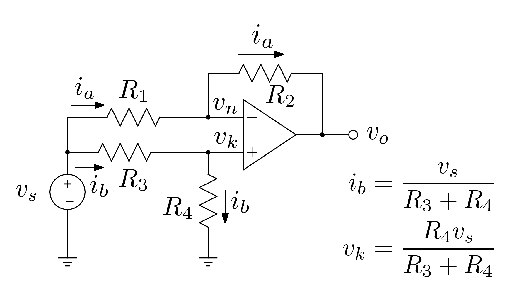
\includegraphics[scale=0.90]{subtractorExample}
\caption{منفی کار کا مشترکہ داخلی مزاحمت}
\label{شکل_منفی_کار_مشترکہ_داخلی_مزاحمت}
\end{figure}
حل:
مشترکہ داخلی مزاحمت حاصل کرنے کی خاطر دونوں داخلی سروں  کو آپس میں جوڑتے ہوئے ان پر مشترکہ اشارہ \عددی{v_s} لاگو کیا جاتا ہے۔اشارے سے \عددی{i_a} اور \عددی{i_b} برقی رو منفی کار میں داخل ہوں گے۔مشترکہ مزاحمت داخلی برقی دباو اور داخلی برقی رو کے مجموعہ کی شرح کو کہتے ہیں یعنی
\begin{align*}
R_{\textup{مشترک}}=\frac{v_s}{i_a+i_b}
\end{align*} 
آئیں داخلی مزاحمت کو پہلے حساب و کتاب سے حاصل کریں۔تمام مزاحمت \عددی{R} کے برابر ہونے کی صورت میں
\begin{align*}
v_0=0\\
v_k=\frac{v_s}{2}\\
v_n=\frac{v_s}{2}
\end{align*}
حاصل ہوتے ہیں۔لہٰذا
\begin{align*}
i_a=\frac{v_s-v_n}{R}=\frac{v_s}{2R}\\
i_b=\frac{v_s-v_k}{R}=\frac{v_s}{2R}\\
i_a+i_b=\frac{v_s}{R}
\end{align*}
اور یوں
\begin{align*}
R_{\textup{داخلی}}=R
\end{align*}
حاصل ہوتا ہے۔

اس جواب کو یوں بھی حاصل کیا جا سکتا ہے۔حسابی ایمپلیفائر کے دونوں داخلی سروں  پر داخلی برقی رو صفر ہوتی ہے۔\عددی{v_k} پر داخلی برقی رو صفر  ہونے کی وجہ سے اسے کھلے سرے تصور کیا جا سکتا ہے۔اس طرح  \عددی{R_3} اور \عددی{R_4} کو \عددی{v_s} اور برقی زمین کے مابین سلسلہ وار جڑا تصور کیا جا سکتا ہے۔تمام مزاحمت برابر ہونے کی وجہ سے \عددی{v_o=\SI{0}{\volt}} ہے لہٰذا اسے برقی زمین تصور کیا جا سکتا ہے۔\عددی{v_n} پر برقی رو صفر ہونے کی وجہ سے اس داخلی سرے  کو بھی کھلے سرے تصور کیا جا سکتا ہے۔یوں \عددی{R_1} اور \عددی{R_2} کو بھی \عددی{v_s} اور برقی زمین کے مابین سلسلہ وار جڑا تصور کیا جا سکتا ہے۔اس طرح سلسلہ وار جڑے \عددی{R_1} اور \عددی{R_2} کو سلسلہ وار جڑے \عددی{R_3} اور \عددی{R_4} کے متوازی تصور کیا جا سکتا ہے لہٰذا
\begin{align*}
\frac{1}{R_{\text{داخلی}}}&=\frac{1}{R_1+R_2}+\frac{1}{R_3+R_4}=\frac{1}{2R}+\frac{1}{2R}=\frac{1}{R}\\
R_{\text{داخلی}}&=R
\end{align*}
حاصل ہوتا ہے۔

تمام مزاحمت مختلف ہونے کی صورت میں مساوات \حوالہ{مساوات_حسابی_منفی_کار} سے خارجی اشارہ  یوں حاصل ہوتا ہے۔
\begin{align*}
v_o=\left[\left(\frac{R_1+R_2}{R_3+R_4} \right)\frac{R_4}{R_1}-\frac{R_2}{R_1} \right]v_s
\end{align*}
حسابی ایمپلیفائر کے دونوں داخلی سروں  پر داخلی برقی رو صفر ہونے کی وجہ سے \عددی{R_1} اور \عددی{R_2} میں یکساں برقی رو \عددی{i_a} پایا جائے گا۔اسی طرح \عددی{R_3} اور \عددی{R_4} میں \عددی{i_b} پایا جائے گا جہاں
\begin{align*}
i_a&=\frac{v_s-v_0}{R_1+R_2}\\
&=v_s\left[\frac{1}{R_1+R_2}-\frac{R_4}{R_1 \left(R_3+R_4 \right)}+\frac{R_2}{R_1 \left(R_1+R_2 \right)} \right]\\
&=\frac{R_3 v_s}{R_1\left(R_3+R_4 \right)}\\
i_b&=\frac{v_s}{R_3+R_4}
\end{align*}
کے برابر ہیں۔یوں
\begin{align*}
R_{\text{داخلی}}=\frac{v_s}{i_a+i_b}=\frac{R_1 \left(R_3+R_4 \right)}{R_1+R_3}
\end{align*}
حاصل ہوتا ہے۔

اسی جواب کو قدر آسان طریقے سے یوں حاصل کیا جا سکتا ہے۔حسابی ایمپلیفائر کے مثبت داخلی سرے  کو کھلے سرے تصور کیا جا سکتا ہے۔اس طرح \عددی{R_3} اور \عددی{R_4} کو \عددی{v_s} اور برقی زمین کے مابین دو سلسلہ وار جڑے مزاحمت تصور کیا جا سکتا ہے۔ان دو مزاحمتوں میں برقی دباو کے تقسیم سے
\begin{align*}
v_k=\frac{R_4 v_s}{R_3+R_4}
\end{align*}
حاصل ہوتا ہے۔اسی طرح ان میں برقی رو
\begin{align*}
i_b=\frac{v_s}{R_3+R_4}
\end{align*}
حاصل ہوتا ہے۔\عددی{v_k=v_n} ہونے کی بدولت \عددی{v_n} بھی یہی ہو گا۔لہٰذا \عددی{R_1} میں برقی رو
\begin{align*}
i_a&=\frac{v_s-v_n}{R_1}=\frac{v_s-\frac{R_4 v_s}{R_3+R_4}}{R_1}
\end{align*}
ہو گا۔ان دو برقی رو سے داخلی مزاحمت حاصل ہوتا ہے۔\عددی{v_n} کی قیمت \عددی{v_k} تعین کرتا ہے۔چونکہ \عددی{v_k} کا دارومدار مزاحمت \عددی{R_3} اور \عددی{R_4} پر ہے  جبکہ \عددی{i_a} کا دارومدار \عددی{v_n} اور \عددی{R_1} پر ہے لہٰذا \عددی{i_a} اور \عددی{i_b} دونوں پر \عددی{R_2} کا کوئی اثر نہیں۔اسی لئے داخلی مزاحمت میں \عددی{R_2} کا کوئی کردار نہیں۔
\انتہا{مثال}
%==============
\ابتدا{مثال} \شناخت{مثال_حسابی_منفی_مزاحمت_غلطی}
\اصطلاح{منفی کار} کے تمام مزاحمت برابر ہونے کی صورت میں دونوں داخلی سروں  پر مشترکہ داخلی اشارہ \عددی{v_s} مہیا کرنے سے \عددی{v_0=\SI{0}{\volt}} حاصل ہوتا ہے۔اس صورت میں منفی کار کی مشترکہ افزائش صفر حاصل ہوتی ہے۔\عددی{\SI{6.8}{\kilo \ohm} \pm \SI{5}{\percent}} کے مزاحمت استعمال کرتے ہوئے ایمپلیفائر کی خراب سے خراب تر مشترکہ افزائش کیا ممکن ہے۔مشترکہ افزائش جتنی زیادہ ہو اتنا ہی اسے خراب سمجھا جاتا ہے۔ 

حل:
مساوات \حوالہ{مساوات_حسابی_منفی_کار} کے مطابق مشترکہ داخلی اشارے کی صورت (\عددی{v_{s2}=v_{s1}=v_s}) میں  مشترکہ افزائش
\begin{align*}
\frac{v_o}{v_s}&=\left(\frac{R_1+R_2}{R_3+R_4} \right) \frac{R_4}{R_1}-\frac{R_2}{R_1}\\
&=\frac{R_1 R_4-R_2R_3}{R_1 \left(R_3+R_4 \right)}\\
&=\frac{1-\frac{R_2R_3}{R_1 R_4}}{1+\frac{R_3}{R_4}}
\end{align*}
حاصل ہوتی ہے۔اس مساوات میں \عددی{v_o} کی زیادہ سے زیادہ قیمت اس صورت حاصل ہو گی جب \عددی{\tfrac{R_3}{R_4}} اور  \عددی{\tfrac{R_2 R_3}{R_1R_4}}  کے قیمت کم سے کم ہوں۔\عددی{\tfrac{R_3}{R_4}} کی قیمت کم سے کم تب ہو گی جب \عددی{R_3} پانچ فی صد کم اور \عددی{R_4} پانچ فی صد زیادہ ہو یعنی جب \عددی{R_3=\SI{6.46}{\kilo \ohm}} اور \عددی{R_4=\SI{7.14}{\kilo \ohm}} ہوں۔اسی طرح \عددی{\tfrac{R_2 R_3}{R_1R_4}} کی قیمت کم سے کم تب ہو گی جب \عددی{R_2=\SI{6.46}{\kilo \ohm}} اور \عددی{R_1=\SI{7.14}{\kilo \ohm}} ہوں گے۔ان قیمتوں کے استعمال سے خراب سے خراب تر مشترکہ افزائش
\begin{align*}
\frac{v_o}{v_s}=\frac{1-\frac{6.46 \times 6.46}{7.14 \times 7.14}}{1+\frac{6.46}{7.14}}=\SI{0.095238}{\volt \per \volt}
\end{align*}
حاصل ہوتی ہے۔

\انتہا{مثال}
%============
\ابتدا{مثال}
مثال \حوالہ{مثال_حسابی_منفی_مزاحمت_غلطی} میں تمام مزاحمت مختلف ہونے کی صورت میں مزاحمت کے قیمت میں غلطی کی وجہ سے خراب تر مشترکہ افزائش کی عمومی جواب حاصل کریں۔

حل:
گزشتہ مثال میں 
\begin{align*}
\frac{v_o}{v_s}=\frac{1-\frac{R_2R_3}{R_1 R_4}}{1+\frac{R_3}{R_4}}
\end{align*}
حاصل کی گئی۔جیسا وہاں بتلایا گیا \عددی{R_2} اور \عددی{R_3} کے قیمت کم سے کم یعنی \عددی{\left(1-\epsilon \right) R_2} اور \عددی{\left(1-\epsilon \right) R_3} جبکہ \عددی{R_1} اور \عددی{R_4} کے قیمت زیادہ سے زیادہ یعنی \عددی{\left(1+\epsilon \right) R_1} اور
 \عددی{\left(1+\epsilon \right) R_4} ہونے ہوں گے۔اس طرح
\begin{align*}
\frac{v_o}{v_s}=\frac{1-\left(\frac{1-\epsilon}{1+\epsilon}\right)^2\frac{R_2R_3}{R_1 R_4}}{1+\left(\frac{1-\epsilon}{1+\epsilon}\right)\frac{R_3}{R_4}}
\end{align*}
حاصل ہوتا ہے۔تمام مزاحمت ایک ہی قیمت کے ہونے کی صورت میں
\begin{align*}
\frac{v_o}{v_s}=\frac{2 \epsilon}{1+\epsilon}
\end{align*}
حاصل ہوتا ہے۔

\انتہا{مثال}

آپ نے حسابی ایمپلیفائر پر مبنی کئی ادوار دیکھے۔یہ ادوار جمع، منفی، تفرق اور تکملہ جیسے حسابی اعمال سرانجام دیتے ہیں یا پھر اشارات کی افزائش کرتے ہیں۔انہیں خوبیوں کی بدولت ہم اسے \اصطلاح{حسابی ایمپلیفائر}  پکارتے ہیں۔\فرہنگ{حسابی ایمپلیفائر}\فرہنگ{OPAMP}\حاشیہب{OPAMP}

\جزوحصہ{جمع و منفی کار}
شکل \حوالہ{شکل_جمع_و_منفی_کار} میں متعدد داخلی سروں  والا \اصطلاح{جمع و منفی کار} دکھایا گیا ہے۔مثبت داخلی سروں  پر \عددی{v_{j1}} تا \عددی{v_{js}} جبکہ منفی داخلی سروں  پر \عددی{v_{m1}} تا \عددی{v_{mn}} اشارات مہیا کئے گئے ہیں۔آئیں اس دور کو حل کریں۔
جوڑ \عددی{v_n} پر کرخوف کے قانون برائے برقی رو سے ہم لکھ سکتے ہیں
\begin{align*}
\frac{v_n-v_{m1}}{R_{m1}}+\frac{v_n-v_{m2}}{R_{m2}} \cdots +\frac{v_n-v_{mn}}{R_{mn}}+\frac{v_n-v_o}{R_0}=0\\
v_n \left(\frac{1}{R_{m1}}+\frac{1}{R_{m2}}\cdots +\frac{1}{R_{mn}}+\frac{1}{R_0} \right)=\frac{v_{m1}}{R_{m1}}+\frac{v_{m2}}{R_{m2}}\cdots +\frac{v_{mn}}{R_{mn}}+\frac{v_o}{R_0}
\end{align*}
جس میں
\begin{align*}
\frac{1}{R_{m1}}+\frac{1}{R_{m2}}\cdots +\frac{1}{R_{mn}}=\frac{1}{R_m}
\end{align*}
لکھتے ہوئے
\begin{align*}
v_n \left(\frac{1}{R_m}+\frac{1}{R_0} \right)=\frac{v_{m1}}{R_{m1}}+\frac{v_{m2}}{R_{m2}}\cdots +\frac{v_{mn}}{R_{mn}}+\frac{v_o}{R_0}\\
v_n=\left(\frac{R_mR_0}{R_m+R_0} \right)\left(\frac{v_{m1}}{R_{m1}}+\frac{v_{m2}}{R_{m2}}\cdots +\frac{v_{mn}}{R_{mn}}+\frac{v_o}{R_0} \right)
\end{align*}
حاصل ہوتا ہے۔اسی طرح جوڑ \عددی{v_k} کے لئے حل کرتے ہیں۔
\begin{align*}
\frac{v_k-v_{j1}}{R_{j1}}+\frac{v_k-v_{j2}}{R_{j2}}\cdots +\frac{v_k-v_{js}}{R_{js}}=0\\
v_k \left(\frac{1}{R_{j1}}+ \frac{1}{R_{j2}}\cdots + \frac{1}{R_{js}}\right)=\frac{v_{j1}}{R_{j1}}+\frac{v_{j2}}{R_{j2}}\cdots+\frac{v_{js}}{R_{js}}
\end{align*}
جس میں
\begin{align*}
\frac{1}{R_{j1}}+ \frac{1}{R_{j2}}\cdots + \frac{1}{R_{js}}=\frac{1}{R_{j}}
\end{align*}
استعمال کرتے ہوئے 
\begin{align*}
v_k=\frac{R_j }{R_{j1}}v_{j1}+\frac{R_j }{R_{j2}}v_{j2}\cdots+\frac{R_j }{R_{js}}v_{js}
\end{align*}
حاصل ہوتا ہے۔\عددی{v_n=v_k} لکھتے ہوئے \عددی{v_o} کے لئے حل کرتے ہوئے حاصل ہوتا ہے۔
\begin{align} \label{مساوات_حسابی_جمع_و_منفی_کار}
v_0&=\left( 1+\frac{R_0}{R_m}\right)\left(\frac{R_j }{R_{j1}}v_{j1}+\frac{R_j }{R_{j2}}v_{j2}\cdots \right. \\
& \qquad  \qquad \left. \cdots +\frac{R_j }{R_{js}}v_{js} \right)-\left(\frac{R_0}{R_{m1}}v_{m1}+\frac{R_0}{R_{m2}}v_{m2}\cdots +\frac{R_0}{R_{mn}}v_{mn}\right)
\end{align}

%
\begin{figure}
\centering
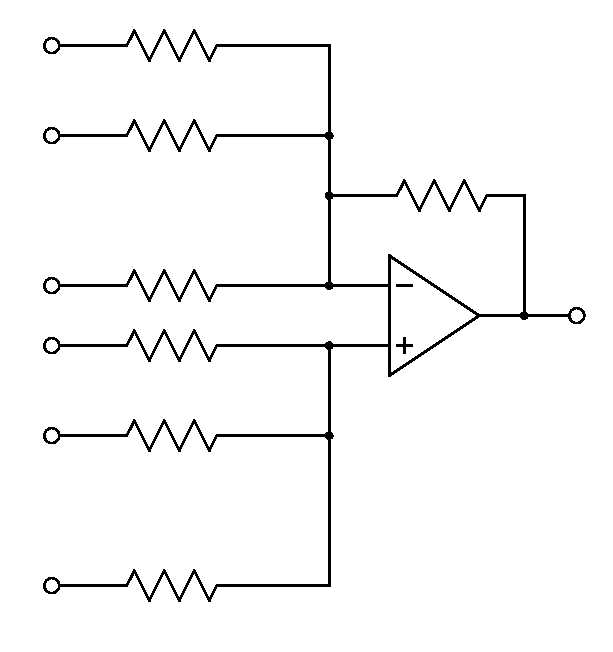
\includegraphics[scale=0.90]{adderSubtractorExample}
\caption{جمع و منفی کار}
\label{شکل_جمع_و_منفی_کار}
\end{figure}

\جزوحصہ{آلاتی ایمپلیفائر}

حسابی ایمپلیفائر پر تبصرہ کرتے ہوئے \اصطلاح{آلاتی ایمپلیفائر}\فرہنگ{آلاتی ایمپلیفائر}\فرہنگ{amplifier!instrumentation}\حاشیہب{instrumentation amplifier} کا ذکر کرنا لازم ہے۔\اصطلاح{آلاتی ایمپلیفائر} باریک اور حساس اشارات کے حصول کے لئے استعمال کیا جاتا ہے۔موجودہ دور میں ہر قسم کے طبعی متغیرات کو برقی اشارات میں تبدیل کر کے ان پر کمپیوٹر کی مدد سے غور کیا جاتا ہے۔آپ \اصطلاح{برقی قلب نگار}\فرہنگ{برقی!قلب نگار}\فرہنگ{ecg}\حاشیہب{ecg} سے بخوبی واقف ہوں گے جو دل کے کارکردگی کے اشارات کھینچتا ہے۔\اصطلاح{برقی قلب نگار} کو \اصطلاح{آلاتی ایمپلیفائر} کے مدد سے ہی بنایا جاتا ہے۔\حاشیہد{آج مورخہ 21 مارچ 2014 کو میری بیٹی عفت بریخنہ  نے انجنیئرنگ کے آخری سال کے پڑھائی کے دوران آلاتی ایمپلیفائر سے برقی قلب نگار بناتے ہوئے دل کی دھڑکن کے اشارات حاصل کئے۔}

ان حساس اشارات کے حصول کے لئے زیادہ سے زیادہ \اصطلاح{داخلی برقی رکاوٹ}\فرہنگ{داخلی برقی رکاوٹ}\حاشیہب{input impedance}  والے ادوار استعمال کئے جاتے ہیں۔ایسے جگہوں پر عموماً \اصطلاح{آلاتی ایمپلیفائر} استعمال کیا جاتا ہے جس کا داخلی برقی رکاوٹ لامحدود تصور کیا جا سکتا ہے۔آلاتی ایمپلیفائر  کو شکل \حوالہ{شکل_آلاتی_ایمپلیفائر} میں دکھایا گیا ہے۔

\begin{figure}
\centering
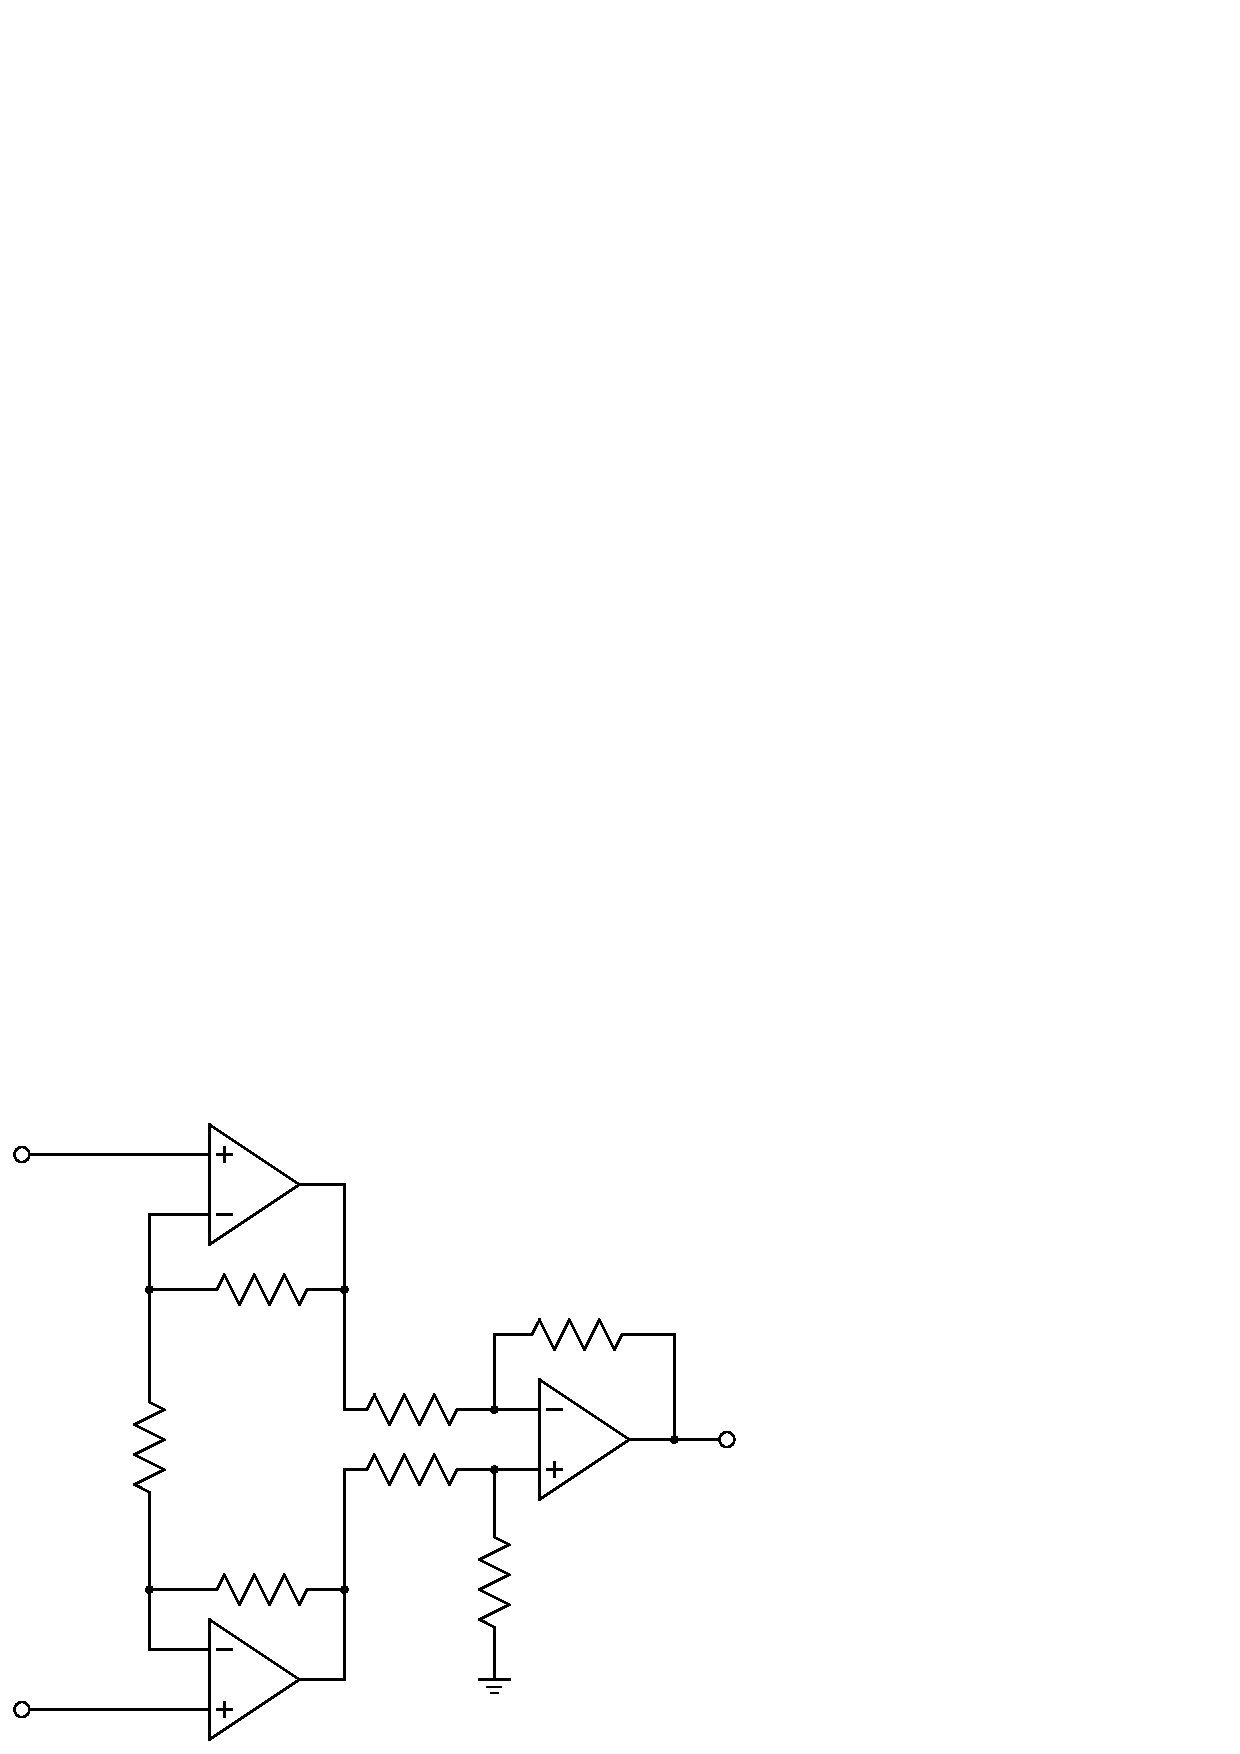
\includegraphics[scale=0.90]{instrumentationAmplifier}
\caption{آلاتی ایمپلیفائر}
\label{شکل_آلاتی_ایمپلیفائر}
\end{figure}
اس دور میں  \عددی{v_1} اور \عددی{v_2} داخلی اشارات ہیں۔کسی بھی حسابی ایمپلیفائر کے داخلی سروں پر برقی دباو برابر رہتا ہے۔یوں \عددی{v_{n1}=v_{k1}=v_1} اور  \عددی{v_{n2}=v_{k2}=v_2} ہو گا۔اس طرح مزاحمت \عددی{R_1} کے نیچے جانب سرے پر برقی دباو کی قیمت \عددی{v_2} اور اس کے اوپر جانب سرے پر برقی دباو کی قیمت \عددی{v_1} ہو گی۔یوں \عددی{R_1} کے سروں کے مابین برقی دباو کی قیمت \عددی{(v_2-v_1)} ہو گی اور اس میں برقی رو
\begin{align}
i_{R_1}=\frac{v_2-v_1}{R_1}
\end{align}
ہو گی۔

جوڑ \عددی{v_{n1}}  پر کرخوف کے قانون برائے برقی رو لاگو کرنے سے ثابت ہوتا ہے کہ اس جوڑ پر نسب \عددی{R_2} میں \عددی{i_{R_1}} کے برابر برقی رو گزرے گی جسے شکل میں تیر کے نشان سے دکھایا گیا ہے۔اسی طرح جوڑ \عددی{v_{n2}} پر کرخوف کے قانون سے ثابت ہوتا ہے کہ اس جوڑ پر نسب \عددی{R_2} میں بھی \عددی{i_{R_1}} گزرے گی جسے تیر کے نشان سے دکھایا گیا ہے۔اس طرح \عددی{i_{R_1}} تین سلسلہ وار جڑی مزاحمت \عددی{R_2} ، \عددی{R_1} اور  \عددی{R_2} سے گزرتی ہے۔ان سلسلہ وار جڑے مزاحمتوں کے آخری سروں کے مابین برقی دباو کو یوں لکھ سکتے ہیں۔
\begin{gather}
\begin{aligned}
v_{o2}-v_{o1}&= i_{R_1} \times \left (R_2+R_1+R_2 \right )\\
&=\frac{\left (v_2-v_1 \right )}{R_1} \left (R_1+2 R_2 \right )\\
&=\left (1+\frac{2 R_2}{R_1}\right ) \left (v_2-v_1 \right )
\end{aligned}
\end{gather}
اس برقی دباو کو خارجی جانب منفی کار کو مہیا کیا جاتا ہے اور یوں 
\begin{align}
v_o = \frac{R_4}{R_3}\left (v_{o2}-v_{o1} \right ) =\frac{R_4}{R_3} \left (1+\frac{2 R_2}{R_1} \right ) \left (v_2-v_1 \right )
\end{align}
جو کہ آلاتی ایمپلیفائر کی درکار مساوات ہے۔

\ابتدا{مثال}
ایک آلاتی ایمپلیفائر میں
\begin{align*}
R_1=\SI{500}{\ohm} \hspace{5mm} R_2=\SI{50}{\kilo \ohm}\\
R_3=\SI{10}{\kilo \ohm} \hspace{5mm} R_4=\SI{10}{\kilo \ohm}\\
v_2=4+0.003 \sin \omega t\\
v_1=4-0.003 \sin \omega  t
\end{align*}
ہیں۔آلاتی ایمپلیفائر کے ہر جوڑ پر برقی دباو حاصل کریں۔\اصطلاح{مشترک اشارہ رد کرنے کی صلاحیت} \عددی{CMRR} حاصل کریں۔

حل:

دونوں داخلی سروں  پر یکساں برقی دباو کو مشترکہ برقی دباو کہتے ہیں جبکہ دونوں داخلی سروں  کے مابین برقی دباو کو تفرق برقی دباو کہتے ہیں۔یوں
\begin{align*}
v_{\text{مشترک}}&=\SI{4}{\volt}\\
v_{\textup{تفرق}}&=0.06 \sin \omega t
\end{align*}
ہیں۔یوں انہیں
\begin{align*}
v_2=v_{\text{مشترک}}+ \frac{v_{\text{تفرق}}}{2}\\
v_1=v_{\text{مشترک}}-\frac{v_{\text{تفرق}}}{2}
\end{align*}
لکھا جا سکتا ہے۔

جوڑ \عددی{v_{n1}} پر \عددی{v_1} جبکہ جوڑ \عددی{v_{n2}} پر \عددی{v_2} پایا جائے گا۔یوں \عددی{R_1} میں برقی رو کی قیمت
\begin{align*}
I_{R1}=\frac{\left(4+0.003 \sin \omega t \right)-\left(4-0.003 \sin \omega t \right)}{500}=12 \times 10^{-6} \sin \omega t
\end{align*}
 ہو گی۔یوں مزاحمت \عددی{R_2} کے دو سروں کے مابین برقی دباو  کی قیمت
\begin{align*}
12 \times 10^{-6} \sin \omega t \times 50 \times 10^3=0.6 \sin \omega t
\end{align*}
ہو گی۔نچلے \عددی{R_2} میں برقی رو کی سمت مزاحمت کے دائیں سرے سے بائیں سرے کی جانب ہے۔یوں اس کا دایاں سرا مثبت جبکہ بایاں سرا منفی ہو گا۔چونکہ ان سروں پر برقی دباو کو \عددی{v_{o2}} اور \عددی{v_{n2}} کہا گیا ہے لہٰذا
\begin{align*}
v_{o2}-v_{n2}&=0.6 \sin \omega t\\
v_{o2}&=4+0.003 \sin \omega t +0.6 \sin \omega t\\
&=4+0.603 \sin \omega t
\end{align*}
ہو گا۔اسی طرح اوپر والے \عددی{R_2} میں برقی رو کی سمت \عددی{v_{n1}} سے \عددی{v_{o1}} کے جانب ہے لہٰذا
\begin{align*}
v_{n1}-v_{o1}&=0.6 \sin \omega t\\
v_{o1}&=4-0.003 \sin \omega t -0.6 \sin \omega t\\
&=4-0.603 \sin \omega t
\end{align*}
حاصل ہو گا۔یہاں رک کر نتائج پر غور کریں۔مشترکہ اشارہ جوں کا توں ہے جبکہ تفرق اشارہ دونوں خارجی سروں  پر  بڑھ گیا ہے۔\عددی{v_{o2}} اور \عددی{v_{o1}} کو منفی کار کے حوالے کیا جاتا ہے۔منفی کار  کے مثبت داخلی سرا \عددی{v_k} پر کرخوف کے قانون برائے برقی رو لکھتے ہوئے
\begin{align*}
&\frac{v_k-v_{o2}}{R_3}+\frac{v_k}{R_4}=0\\
v_k&=\left(\frac{R_4}{R_3+R_4} \right) v_{o2}\\
&=2+0.3015 \sin \omega t
\end{align*}
حاصل ہوتا ہے۔\عددی{v_n} اور \عددی{v_k} برابر ہونے کی وجہ سے \عددی{v_n} بھی یہی ہو گا۔مندرجہ بالا جواب \عددی{R_3} اور \عددی{R_4} کو سلسلہ وار \عددی{v_{o2}} اور برقی زمین کے مابین جڑا تصور کرتے ہوئے برقی دباو کے تقسیم کی مساوات سے بھی حاصل ہوتا ہے۔منفی کار کا خارجی اشارہ
\begin{align*}
v_o&=\frac{R_4}{R_3}{\left(v_{o2}-v_{o1} \right)}\\
&=\frac{10000}{10000} \left[\left(4+0.603 \sin \omega t\right)-\left(4-0.603 \sin \omega t \right) \right]\\
&=1.206 \sin \omega t
\end{align*}
حاصل ہوتا ہے۔

چونکہ خارجی اشارے میں مشترکہ اشارے کا نام و نشان تک نہیں لہٰذا مشترکہ افزائش صفر کے برابر ہے یعنی \عددی{A_m=0} جبکہ تفرقی افزائش کو مندرجہ بالا مساوات سے یوں حاصل کیا جا سکتا ہے۔
\begin{align*}
A_d=\frac{v_o}{v_d}=\frac{1.206 \sin \omega t}{0.06 \sin \omega t}=20.1 \, \si{\volt\per\volt}
\end{align*}
اس طرح مشترکہ اشارہ رد کرنے کی صلاحیت
\begin{align*}
CMRR=\frac{A_d}{A_m}=\infty
\end{align*}
حاصل ہوتا ہے۔
\انتہا{مثال}
%======================
اس مثال میں آلاتی ایمپلیفائر نے مشترکہ اشارے کو مکمل رد کرتے ہوئے تفرق اشارے کو \عددی{201} گنا بڑھایا۔ یہاں اس بات پر توجہ دیتے ہوئے ذھن نشین کریں کہ مزاحمتوں کے قیمتیں جس طرح بھی رکھی جائیں \عددی{v_{o2}} اور \عددی{v_{o1}} میں کسی صورت بھی مشترکہ اشارہ بڑھتا نہیں۔ یہ جوں کا توں ان دو خارجی سروں  پر پایا جاتا ہے۔ آلاتی ایمپلیفائر کا دوسرا حصہ یعنی \اصطلاح{منفی کار} \عددی{v_{o2}} سے \عددی{v_{o1}} منفی کرتے ہوئے مشترکہ اشارے کو مکمل طور رد کر دیتا ہے۔ تفرق اشارے کو آلاتی ایمپلیفائر کے دونوں حصے بڑھانے کی صلاحیت رکھتے ہیں۔اگلے مثال میں ان حقائق پر مزید غور کیا جائے گا۔

آلاتی ایمپلیفائر میں دونوں مزاحمت جنہیں \عددی{R_2} لکھا گیا ہے کے قیمتیں برابر رکھی جاتی ہیں۔البتہ مزاحمت کے قیمتوں میں غلطی کی بنا پر ان کی قیمت
 \عددی{\left(1 - \epsilon \right) R_2} تا  \عددی{\left(1 + \epsilon \right) R_2} ممکن ہوتی ہیں۔مزاحمت کے قیمت میں \عددی{\SI{\mp 1}{\percent}} غلطی کی صورت میں \عددی{\epsilon =0.01} کے برابر ہو گا۔شکل \حوالہ{شکل_آلاتی_ایمپلیفائر_مثال} میں آلاتی ایمپلیفائر کو دوبارہ دکھاتے ہوئے ان حقائق کو واضح کیا گیا ہے جہاں ایک مزاحمت کو \عددی{R_2} جبکہ دوسرے کو \عددی{R_2'} لکھا گیا ہے۔اسی طرح\عددی{R_3} اور \عددی{R_4} کو بھی دکھایا گیا ہے۔
\begin{figure}
\centering
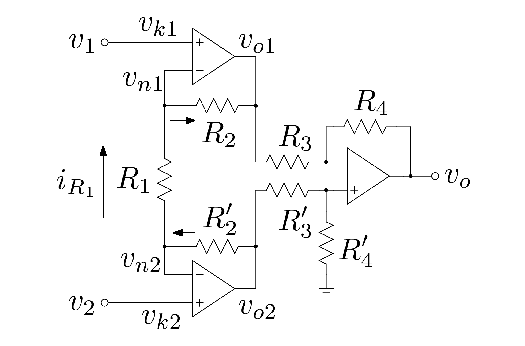
\includegraphics[scale=0.90]{instrumentationAmplifierExample}
\caption{آلاتی ایمپلیفائر کی مثال}
\label{شکل_آلاتی_ایمپلیفائر_مثال}
\end{figure}

\ابتدا{مثال}
\begin{itemize}
\item
شکل \حوالہ{شکل_آلاتی_ایمپلیفائر_مثال} کو استعمال کرتے ہوئے آلاتی ایمپلیفائر کے مشترکہ افزائش \عددیء{A_m} اور تفرق افزائش \عددی{A_d} کے مساوات حاصل کریں۔
\item
مزاحمتوں کے قیمت مکمل طور درست ہونے کی صورت میں \عددی{A_m=0} اور یوں \عددی{CMRR=\infty} حاصل ہوتا ہے۔مندرجہ ذیل \عددی{\SI{\mp 1}{\percent}} مزاحمت استعمال کرتے ہوئے \اصطلاح{مشترکہ اشارہ رد کرنے کی صلاحیت} \عددی{CMRR} کی کمتر قیمت کیا ممکن ہے۔
\begin{align*}
R_1=\SI{10}{\kilo \ohm} \hspace{5mm} R_2=R_2'=\SI{100}{\kilo \ohm}\\
R_3=R_3'=\SI{10}{\kilo \ohm} \hspace{5mm} R_4=R_4'=\SI{10}{\kilo \ohm}
\end{align*}
%
\item
\عددی{R_1=\SI{1}{\kilo \ohm}} کر دینے سے جواب کیا حاصل ہوتا ہے۔
\item
مزاحمت کے ان قیمتوں سے \اصطلاح{مشترکہ اشارہ رد کرنے کی صلاحیت} \عددی{CMRR} کی کمتر قیمت کیا ممکن ہے۔
\begin{align*}
R_1=\SI{10}{\kilo \ohm} \hspace{5mm} R_2=R_2'=\SI{10}{\kilo \ohm}\\
R_3=R_3'=\SI{10}{\kilo \ohm} \hspace{5mm} R_4=R_4'=\SI{100}{\kilo \ohm}
\end{align*}

\end{itemize}

حل:
\begin{itemize}
\item
مشترکہ اشارے کو \عددی{v_c} جبکہ تفرق اشارے کو \عددی{v_d} لکھتے ہوئے
\begin{align*}
v_2=v_c+\frac{v_d}{2}\\
v_1=v_c-\frac{v_2}{2}
\end{align*}
لیتے ہوئے حل کرتے ہیں۔ 
\item
آلاتی ایمپلیفائر کے پہلے حصے کے لئے ہم لکھ سکتے ہیں۔
\begin{gather}
\begin{aligned}\label{مساوات_آلاتی_پہلا_حصہ}
i_{R1}&=\frac{v_{n2}-v_{n1}}{R_1}=\frac{v_2-v_1}{R_1}\\
v_{o2}&=v_{n2}+i_{R1} R_2'=\left(1+\frac{R_2'}{R_1} \right) v_2-\frac{R_2'}{R_1} v_1\\
&=\left(1+\frac{R_2'}{R_1} \right) \left(v_c+\frac{v_d}{2} \right)-\frac{R_2'}{R_1} \left(v_c-\frac{v_2}{2} \right)\\
&=v_c+\left(\frac{1}{2}+\frac{R_2'}{R_1}\right) v_d\\
v_{o1}&=v_n1-i_{R1} R_2=-\frac{R_2}{R_1} v_2+\left(1+\frac{R_2}{R_1} \right) v_1\\
&=-\frac{R_2}{R_1} \left(v_c+\frac{v_d}{2} \right)+\left(1+\frac{R_2}{R_1} \right) \left(v_c-\frac{v_2}{2}\right)\\
&=v_c-\left(\frac{1}{2}+\frac{R_2}{R_1} \right) v_d
\end{aligned}
\end{gather}
آلاتی ایمپلیفائر کے دوسرے حصے کو مساوات \حوالہ{مساوات_حسابی_منفی_کار} بیان کرتا ہے جس  میں مزاحمتوں کے موجودہ نام استعمال کرتے ہوئے یہاں دوبارہ پیش کرتے ہیں۔
\begin{align*}
v_o=\left(\frac{1+\frac{R_4}{R_3}}{1+\frac{R_3'}{R_4'}} \right) v_{o2}-\frac{R_4}{R_3}v_{o1}
\end{align*}
اس میں مساوات \حوالہ{مساوات_آلاتی_پہلا_حصہ} کا استعمال کرتے ہوئے
\begin{align*}
v_o&=\left(\frac{1+\frac{R_4}{R_3}}{1+\frac{R_3'}{R_4'}} \right) \left[v_c+\left(\frac{1}{2}+\frac{R_2'}{R_1}\right) v_d \right]-\frac{R_4}{R_3}\left[ v_c-\left(\frac{1}{2}+\frac{R_2}{R_1} \right) v_d\right]\\
&=\left[\frac{1+\frac{R_4}{R_3}}{1+\frac{R_3'}{R_4'}} -\frac{R_4}{R_3} \right] v_c +\left[\left(\frac{1+\frac{R_4}{R_3}}{1+\frac{R_3'}{R_4'}} \right)\left(\frac{1}{2}+\frac{R_2'}{R_1} \right) +\frac{R_4 }{R_3 }\left(\frac{1}{2}+\frac{R_2}{R_1} \right)\right]v_d\\
&=A_c v_c +A_d v_d
\end{align*}
جہاں
\begin{align*}
A_c&=\frac{1+\frac{R_4}{R_3}}{1+\frac{R_3'}{R_4'}} -\frac{R_4}{R_3}=\frac{1+\frac{R_4}{R_3}-\frac{R_4}{R_3}-\frac{R_3'R_4}{R_4'R_3}}{1+\frac{R_3'}{R_4'}}=\frac{1-\frac{R_3'R_4}{R_4'R_3}}{1+\frac{R_3'}{R_4'}}\\
A_d&=\left(\frac{1+\frac{R_4}{R_3}}{1+\frac{R_3'}{R_4'}} \right)\left(\frac{1}{2}+\frac{R_2'}{R_1} \right) +\frac{R_4}{R_3 }\left(\frac{1}{2}+\frac{R_2}{R_1} \right)
\end{align*}
ہیں۔
\item
کمتر \عددی{CMRR} اس وقت حاصل ہو گی جب مشترکہ افزائش بلند تر جبکہ تفرق افزائش کمتر ہو یعنی
\begin{align*}
CMRR_{\text{کمتر}}=\abs{\frac{A_d{\text{کمتر}}}{A_c{\text{بلندتر}}}}
\end{align*} 
\عددی{A_c} کی بلند تر قیمت اس وقت حاصل ہو گی جب \عددی{\tfrac{R_3'R_4}{R_4'R_3}} کی قیمت کم سے کم ہو یعنی
\begin{align*}
R_4'=\left(1+0.01 \right) 10000=10100\\
R_3'=\left(1-0.01 \right) 10000=9900\\
R_4=\left(1-0.01 \right) 10000=9900\\
R_3=\left(1+0.01 \right) 10000=10100
\end{align*}
اسی طرح \عددی{A_d} کی کمتر قیمت اس وقت حاصل ہو گی جب
\begin{align*}
R1=(1+0.01)10000=10100\\
R_2'=(1-0.01)100000=99000\\
R_2=(1-0.01)100000=99000
\end{align*}
ہوں۔ان  سے
\begin{align*}
CMRR_{\text{کمتر}}=1030
\end{align*}
حاصل ہوتا ہے۔
\item
\عددی{R_1=\SI{1}{\kilo \ohm}} کرنے سے
\begin{align*}
CMRR_{\text{کمتر}}=9852
\end{align*}
ہو جاتا ہے۔
\item
ان نئے قیمتوں سے
\begin{align*}
R_4'=\left(1+0.01 \right) 100000=101000\\
R_3'=\left(1-0.01 \right) 10000=9900\\
R_4=\left(1-0.01 \right) 100000=99000\\
R_3=\left(1+0.01 \right) 10000=10100\\
R1=(1+0.01)10000=10100\\
R_2=R_2'=(1-0.01)10000=9900
\end{align*}
اور 
\begin{align*}
CMRR_{\text{کمتر}}=814
\end{align*}
حاصل ہوتا ہے۔
\end{itemize}
\انتہا{مثال}
%==============

اس مثال میں دو حقائق سامنے آئے۔پہلا یہ کہ \عددی{A_d} بڑھانے سے \عددی{CMRR} کی کمتر قیمت بڑھتی ہے۔دوسری یہ ہے کہ آلاتی ایمپلیفائر کے \عددی{A_d} کو پہلے حصے سے حاصل کرنا زیادہ بہتر ہے۔
%===================


\حصہ{حسابی ایمپلیفائر کا ناقص پن}

	اب تک حسابی ایمپلیفائر پر مبنی جتنے بھی ادوار پر غور ہوا، ان تمام میں حسابی ایمپلیفائر کو کامل تصور کیا گیا۔اس حصہ میں غیر کامل حسابی ایمپلیفائر پر غور کیا جائے گا۔

\جزوحصہ{حسابی ایمپلیفائر کا لبریز ہونا} \label{جزو_حسابی_ایمپلیفائر_کا_لبریز_ہونا}

حسابی ایمپلیفائر کا \عددی{v_o} ہر صورت مساوات \حوالہ{مساوات_حسابی_کے_خارجی_حدود}  میں دیے گئے حدود کے اندر رہتا ہے۔\عددی{v_o} ان حدود سے تجاوز کرنے کی کوشش کرتے ہی غیر خطی صورت اختیار کر لیتا ہے۔حسابی ایمپلیفائر کے اس غیر خطی عمل کو حسابی ایمپلیفائر کا \اصطلاح{لبریز}\فرہنگ{لبریز}
\فرہنگ{saturation!OPAMP}\حاشیہب{saturation} ہونا کہتے ہیں۔شکل \حوالہ{شکل_حسابی_ایمپلیفائر_کا_لبریز_ہونا} میں یہ عمل دکھایا گیا ہے۔
\begin{figure}
\centering
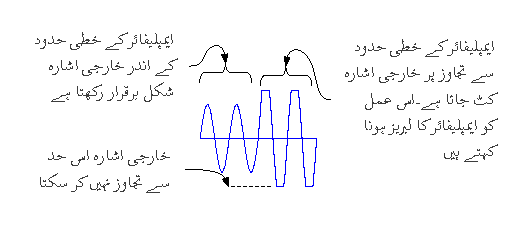
\includegraphics[scale=0.90]{opampSaturation}
\caption{حسابی ایمپلیفائر کا لبریز ہونا}
\label{شکل_حسابی_ایمپلیفائر_کا_لبریز_ہونا}
\end{figure}
\جزوحصہ{حسابی ایمپلیفائر کی رفتار چال}

کوئی بھی اشارہ لامحدود رفتار سے تبدیل نہیں ہو سکتا۔یہی حسابی ایمپلیفائر کے خارجی  اشارے کے لئے بھی درست ہے۔اگر حسابی ایمپلیفائر کو مستطیلی اشارہ بطور داخلی اشارہ فراہم کیا جائے تو اس کا خارجی اشارہ ترچھی شکل کا ہو گا۔آئیں اس عمل کو مستحکم کار کی مدد سے سمجھیں۔اگر \اصطلاح{مستحکم کار} کا شکل \حوالہ{شکل_حسابی_ایمپلیفائر_رفتار_چال}  میں دکھایا مستطیلی داخلی اشارہ فراہم کیا جائے تو اس کا خارجی اشارہ ترچھا ہو گا۔خارجی اشارے کو کسی ایک برقی دباو سے کسی دوسرے برقی دباو کو حاصل کرنے کے لئے وقت درکار ہوتا ہے۔خارجی اشارہ جس رفتار سے حرکت کرتا ہے اسے حسابی ایمپلیفائر کا \اصطلاح{رفتار چال}\فرہنگ{رفتار چال}\فرہنگ{slew rate}\حاشیہب{slew rate} پکارا جائے گا۔\اصطلاح{رفتار چال} کی وضاحت شکل میں کی گئی ہے۔رفتار چال کو عموماً وولٹ فی مائیکرو سیکنڈ \عددی{\si{\volt\per \micro \second}} لکھا جاتا ہے۔
\begin{align}
\textup{رفتار چال}=\abs{\frac{\Delta v}{\Delta t}}
\end{align}
% 
\begin{figure}
\centering
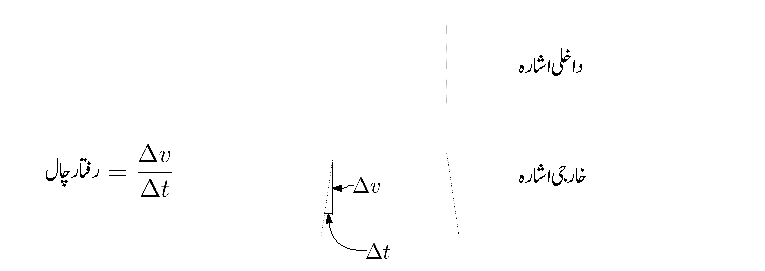
\includegraphics[scale=0.90]{opampSlewRate}
\caption{حسابی ایمپلیفائر کا رفتار چال}
\label{شکل_حسابی_ایمپلیفائر_رفتار_چال}
\end{figure}

سائن نما  اشارہ \عددی{V_p \sin \omega t} کے تفرق کی زیادہ سے زیادہ قیمت \عددی{t=0} پر پائی جاتی ہے یعنی
\begin{align*}
\eval{\od{v_s}{t}}_{t=0}=\eval{\omega V_p \cos \omega t}_{t=0}=\omega V_p
\end{align*}
جب تک یہ مقدار حسابی ایمپلیفائر کے \اصطلاح{رفتار چال} سے کم ہو اس وقت تک حسابی ایمپلیفائر خوش اسلوبی سے اس اشارے کو خارج کرے گا۔جیسے ہی یہ مقدار \اصطلاح{رفتار چال} سے بڑھ جائے، حسابی ایمپلیفائر کے خارجی اشارے میں خلل پیدا ہو جائے گا۔حسابی ایمپلیفائر کے \اصطلاح{رفتار چال} کو اس کی \اصطلاح{پوری طاقت پر تعددی دائرہ کارکردگی}\فرہنگ{پورے طاقت پر دائرہ کارکردگی}\حاشیہب{full power band width} کی شکل میں یوں بیان کیا جاتا ہے
\begin{align}
\omega_{\text{\RL{دائرہ کارکردگی}}}=\frac{\text{\RL{رفتار چال}}}{V_p}\\
f_{\text{\RL{دائرہ کارکردگی}}}=\frac{\text{\RL{رفتار چال}}}{2 \pi V_p}
\end{align}   
جہاں \عددی{V_p} حسابی ایمپلیفائر کی زیادہ سے زیادہ ممکنہ  خارجی برقی دباو ہے۔کم برقی دباو خارج کرتے ہوئے اس تعدد کی قیمت بڑھ جاتی ہے۔یوں \عددی{V_0} برقی دباو خارج کرتے ہوئے
 \begin{align}
\omega_{\text{\RL{بلند تر}}}=\frac{\text{\RL{رفتار چال}}}{V_0}
\end{align}   
ہو گا۔شکل \حوالہ{شکل_حسابی_رفتار_چال_محدود_اشارہ} میں خارجی اشارے پر رفتار چال کا اثر دکھایا گیا ہے۔یہ اشارہ  اپنی اصل صورت کھو کر تکونی شکل اختیار کر گیا ہے جہاں تکون کے اطراف \عددی{رفتار چال} سے بلند اور پست ہو رہے ہیں۔
\begin{figure}
\centering
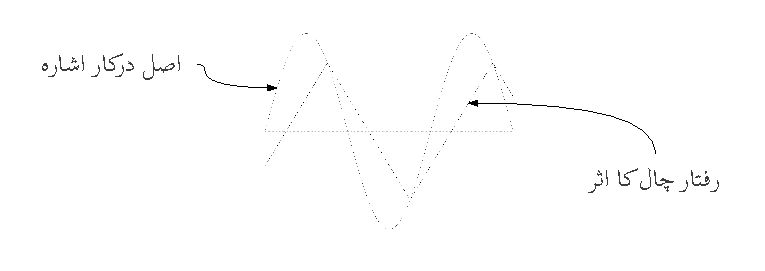
\includegraphics[scale=0.90]{slewRateLimitedSineWave}
\caption{رفتار چال کا اثر}
\label{شکل_حسابی_رفتار_چال_محدود_اشارہ}
\end{figure}
\ابتدا{مثال}
ایک حسابی ایمپلیفائر جس کی \اصطلاح{رفتار چال}  \عددی{\SI{100}{\volt \per \micro \second}} ہے  کا مستحکم کار بنایا جاتا ہے جسے نہایت کم دورانیے والے \عددی{\SI{5}{\volt}} چوٹی کے موٹا {مستطیلی پتلے اشارات}\فرہنگ{مستطیلی پتلا اشارہ}\حاشیہب{pulses}  مہیا کئے جاتے ہیں۔
\begin{itemize}
\item
اشارے کے چوٹی کی کم سے کم وہ دورانیہ \عددی{t_p} دریافت کریں جس پر خارجی اشارہ بھی \عددی{\SI{5}{\volt}} تک پہنچ پاتا ہے۔
\item
اگر داخلی اشارہ متواتر تبدیل ہوتے ہوئے حاصل کردہ دورانیہ \عددی{t_p} کے لئے \عددی{\SI{5}{\volt}} اور اتنے ہی  دورانیے کے لئے \عددی{\SI{0}{\volt}} پر رہتا ہو تو خارجی اشارے کی شکل کیا ہو گی۔
\end{itemize}

حل:
\begin{itemize}
\item
رفتار چال کے مطابق خارجی اشارہ ایک مائیکرو سیکنڈ میں سو وولٹ حاصل کرنے کی صلاحیت رکھتا ہے۔پانچ وولٹ حاصل کرنے کے لئے یوں \عددی{\SI{50}{\nano \second}} درکار ہیں۔داخلی اشارے کی چوٹی کم سے کم \عددی{\SI{50}{\nano \second}} کے لئے برقرار رہے گی تو مستحکم کار کا خارجی اشارہ بھی پانچ وولٹ تک پہنچ جائے گا۔
\item
اس صورت میں جیسے ہی خارجی اشارہ پانچ وولٹ پر پہنچتا ہے اسی لمحہ داخلی اشارہ صفر وولٹ ہو جاتا ہے اور یوں حسابی ایمپلیفائر کا خارجی اشارہ \عددی{\SI{100}{\volt \per \micro \second}} کے رفتار سے اب \عددی{\SI{5}{\volt}} سے \عددی{\SI{0}{\volt}} کی جانب روانہ ہوتا ہے۔یوں خارجی اشارہ تکونی  شکل کا ہو گا جو متواتر \عددی{\SI{50}{\nano \second}} لیتے ہوئے  \عددی{\SI{5}{\volt}} تک اور اسی طرح \عددی{\SI{50}{\nano \second}} لیتے ہوئے  \عددی{\SI{0}{\volt}} کے درمیان ارتعاش کرتا رہے گا۔ 
\end{itemize}
\انتہا{مثال}
%===========
\ابتدا{مثال}
ایک منفی حسابی ایمپلیفائر  \عددی{0.1 \sin \omega t} کا اشارہ تیس گنا بڑھاتا ہے۔اگر حسابی ایمپلیفائر کا رفتار چال \عددی{\SI{1000}{\volt \per \micro \second}} ہو تب داخلی اشارے کی وہ بلند ترین تعدد حاصل کریں جس پر خارجی اشارہ نہ بگڑے۔

حل:
خارجی اشارہ \عددی{-3 \sin \omega t} ہے جس کا تیز ترین رفتار \عددی{t=0} 
\begin{align*}
\abs{-3 \omega \cos \omega t}_{t=0}=3 \omega
\end{align*}
ہے۔یوں 
\begin{align*}
f=\frac{1000 \times 10^6}{2 \times \pi \times 3}=\SI{53}{\mega \hertz}
\end{align*}
وہ بلند ترین تعدد ہے جس کے اشارے کو ایمپلیفائر بالکل درست خارج کر سکتا ہے۔
\انتہا{مثال}

\حصہ{عددی اشارے سے مماثلی اشارے کا حصول} \شناخت{حصہ_حسابی_عددی_سے_مماثل_کار}
شکل \حوالہ{شکل_حسابی_عددی_سے_مماثل_کار} میں عددی اشارے سے مماثل اشارہ حاصل کرنے والا دور دکھایا گیا ہے جسے ہم \اصطلاح{عددی سے مماثل کار}\فرہنگ{عددی سے مماثل کار}\فرہنگ{DAC}\حاشیہب{Digital to Analog Converter (DAC)} کہیں گے۔اس دور کے چار داخلی اشارات  \عددی{d_o} تا \عددی{d_3} ہیں جنہیں انفرادی طور پر برقی زمین یعنی \عددی{\SI{0}{\volt}} یا مثبت برقی دباو یعنی \عددی{\SI{5}{\volt}} کے ساتھ جوڑا جا سکتا ہے۔شکل میں \عددی{d_2=\SI{0}{\volt}} پر جبکہ \عددیء{d_0}، \عددی{d_1} اور \عددی{d_3} کو \عددی{\SI{5}{\volt}} پر دکھایا گیا ہے۔
\begin{figure}
\centering
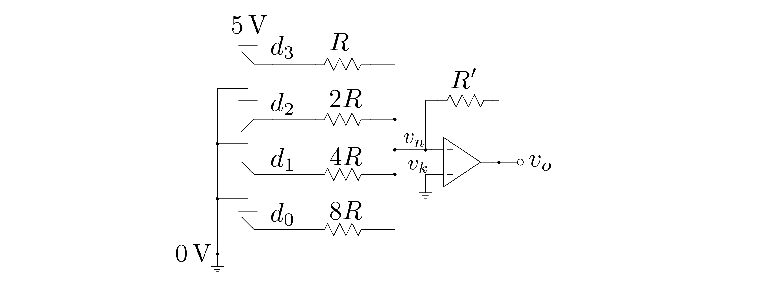
\includegraphics[scale=0.90]{DAC}
\caption{چار بِٹ کا عددی سے مماثل کار}
\label{شکل_حسابی_عددی_سے_مماثل_کار}
\end{figure}
آئیں اس دور کو حل کرتے ہیں۔
\begin{align*}
v_k=0\\
\frac{v_n-d_3}{R}+\frac{v_n-d_2}{2R}+\frac{v_n-d_1}{4R}+\frac{v_n-d_0}{8R}+\frac{v_n-v_o}{R'}=0\\
v_0=-\frac{R'}{8 R} \left(8 d_3+4d_2+2d_1+d_0 \right)
\end{align*}
جسے یوں بہتر طریقے سے لکھا جا سکتا ہے۔
\begin{align} \label{مساوات_حسابی_عددی_سے_مماثل_کار}
v_0=-\frac{R'}{8 R} \left(2^3 d_3+2^2 d_2+2^1 d_1+2^0 d_0 \right)
\end{align}

\اصطلاح{عددی سے مماثل کار} عددی\حاشیہب{digital} متغیرہ لیتے ہوئے اس کا مماثل\حاشیہب{analog} متغیرہ خارج کرتا ہے۔عددی متغیرات کو  \اصطلاح{دہری نظام اعداد}\فرہنگ{دہری نظام اعداد}\حاشیہب{binary number system} میں لکھا جاتا ہے۔\اصطلاح{دہری  نظام اعداد} کے دو ہی ہندسے ہیں یعنی \عددی{0} (صفر) اور \عددی{1} (ایک)۔ \عددی{0}کو \عددی{\SI{0}{\volt}} اور \عددی{1} کو \عددی{\SI{5}{\volt}} سے ظاہر کیا جاتا ہے۔\عددی{d_0} تا \عددی{d_3} کو \عددی{d_3 d_2 d_1 d_0} لکھتے ہوئے چار \اصطلاح{بِٹ}\فرہنگ{بِٹ}\فرہنگ{bit}\حاشیہب{bit} کا دہرا عدد حاصل ہوتا ہے۔یوں شکل میں دکھائی صورت
\begin{align*}
d_3 d_2 d_1 d_0 =1011_2
\end{align*}
کو ظاہر کرتی ہے جو کہ \اصطلاح{اعشاری نظام گنتی}\حاشیہب{decimal number system} میں  گیارہ \عددی{11_{10}} کے برابر ہے۔

اگر تمام داخلی \اصطلاح{دہرے ہندسے} صفر کر دیے جائیں تو  مساوات \حوالہ{مساوات_حسابی_عددی_سے_مماثل_کار} کے مطابق \اصطلاح{عددی سے مماثل کار} \عددی{v_o=\SI{0}{\volt}} خارج کرے گا جبکہ اگر تمام داخلی دہرے ہندسے ایک کر دیے جائیں یعنی انہیں \عددی{\SI{5}{\volt}} سے ظاہر کیا جائے تب دور
\begin{align*}
v_0&=-\frac{R'}{8 R} \left(2^3 \times 5+2^2 \times 5+2^1 \times 5+2^0 \times 5 \right)\\
&=-\frac{R'}{8 R} \left(2^3+2^2 +2^1 +2^0  \right) \times 5\\
&=-\frac{R'}{8 R} \left(8+4 +2 +1 \right) \times 5\\
&=-\frac{R'}{8 R}\times 75
\end{align*}  
خارج کرے گا۔

\عددی{R'} اور \عددی{R} کی قیمت سے درکار قیمت تعین کی جا سکتی ہے۔مثلاً \عددی{R'=\tfrac{8 R}{15}} رکھتے ہوئے مندرجہ بالا مساوات کے مطابق \اصطلاح{عددی سے مماثل کار} \عددی{v_o=\SI{-5}{\volt}} خارج کرے گا۔چونکہ \عددی{d_o} تا \عددی{d_3} کے چار ہندسوں پر مبنی دہرا عدد سولہ \عددی{16_{10}} مختلف قیمتیں ظاہر کر سکتا ہے لہٰذا \اصطلاح{عددی سے مماثل کار} صفر وولٹ تا منفی پانچ وولٹ سولہ مختلف قیمتیں خارج کر سکتا ہے۔

\اصطلاح{عددی سے مماثل کار} میں اسی طرز پر مزید داخلی اشارات  جوڑتے ہوئے زیادہ ہندسوں کا \اصطلاح{عددی سے مماثل کار} بنایا جاتا ہے۔ 

\ابتدا{مثال}
\عددی{R'=\tfrac{8 R}{15}} رکھتے ہوئے \عددی{d_3 d_2 d_1 d_0} کی قیمت \عددی{1010_2} ہونے کی صورت میں \اصطلاح{عددی سے مماثل کار} کتنی برقی دباو خارج کرے گا۔

حل:
\begin{align*}
v_0&=-\frac{R'}{8 R} \left(2^3 \times 5+2^2 \times 0+2^1 \times 5+2^0 \times 0 \right)\\
&=-\frac{R'}{8 R} \left(2^3+2^1  \right) \times 5\\
&=\SI{-3.333}{\volt}
\end{align*}  
\انتہا{مثال}

\جزوحصہ{یک سمت  اندرونی داخلی انحرافی برقی دباو کا مسئلہ}

اگر کامل حسابی ایمپلیفائر کے دونوں داخلی سرے آپس میں جوڑ کر انہیں برقی زمین کے ساتھ جوڑا جائے، یعنی \عددی{v_k=v_n=0} کر دیا جائے، تو ہم توقع کرتے ہیں کہ اس کا خارجی   اشارہ صفر وولٹ کا ہو گا، یعنی \عددی{v_o = A_d v_d =0} ہو گا۔حقیقت میں ایسا نہیں ہوتا\حاشیہد{اس مسئلہ کے پیدا ہونے کی وجوہات پر  حصہ \حوالہ{حصہ_تفرقی_ایمپلیفائر_داخلی_انحرافی_برقی_دباو} میں تفصیلاً تبصرہ کیا جائے گا} اور عموماً اس طرح جڑا حسابی ایمپلیفائر مثبت یا منفی جانب \اصطلاح{لبریز}\فرہنگ{لبریز} پایا جاتا ہے۔ حسابی ایمپلیفائر کے \عددی{v_o} کو صفر وولٹ پر لانے کی خاطر حسابی ایمپلیفائر کے دونوں داخلی سروں کے مابین برقی دباو \عددی{V_{OS}} مہیا کرنا پڑتا ہے۔

	اس حقیقت کو یوں بھی بیان کیا جا سکتا ہے کہ حسابی ایمپلیفائر بناتے وقت پوری کوشش کے باوجود اسے کامل بنانا ناممکن ہوتا ہے اور اس میں کچھ کمی رہ جاتی ہے جس کی وجہ سے اس کا عمل یوں پایا جاتا ہے جیسے اس کے داخلی سروں کے مابین برقی دباو \عددی{V_{OS}}جڑی ہو۔اس خیالی برقی دباو \عددی{V_{OS}} کو ختم کرنے کی خاطر ہمیں اتنی ہی، مگر اُلٹ علامت والی، برقی دباو \عددی{V_{OS}} اس کے دونوں داخلی سروں کے مابین فراہم کرنی پڑتی ہے۔اس خیالی برقی دباو کو \اصطلاح{اندرونی داخلی انحرافی برقی دباو}\فرہنگ{اندرونی داخلی انحرافی برقی دباو}\فرہنگ{input offset voltage}\حاشیہب{input offset voltage}  کہتے ہیں۔شکل \حوالہ{شکل_انحرافی_برقی_دباو_اور_اس_کا_خاتمہ} میں اس کی وضاحت کی گئی ہے۔

	اندرونی داخلی انحرافی برقی دباو کی موجودگی غیر پسندیدہ حقیقت ہے جسے ختم کرنے کی تمام تر کوشش کی جاتی ہے۔حسابی ایمپلیفائر بنانے والے صنعت کار اپنے بنائے گئے حسابی ایمپلیفائر میں پائے جانے والے اندرونی داخلی انحرافی برقی دباو کے حدود کی معلومات فراہم کرتے ہیں۔یہ حدود عموماً \عددی{\SI{\mp 1}{\milli \volt}}  تا \عددی{\SI{\mp 5}{\milli \volt}} تک ہوتے ہیں۔ اندرونی داخلی انحرافی برقی دباو کی علامت نہیں بتلائی جاتی چونکہ قبل از استعمال اس کا جاننا ممکن نہیں ہوتا۔
\begin{figure}
\centering
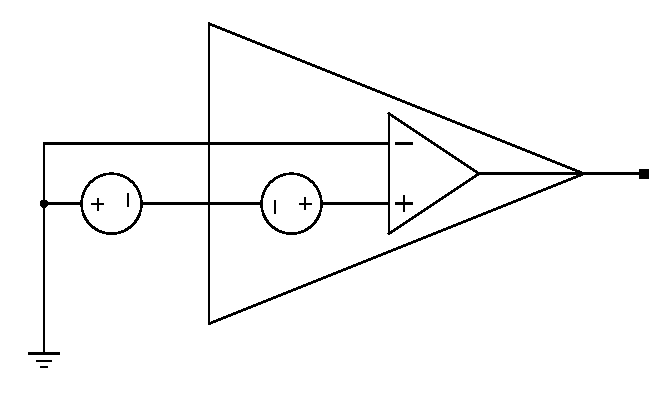
\includegraphics[scale=0.90]{opampInputOffsetVoltage}
\caption{داخلی انحرافی برقی دباو اور اس کا خاتمہ}
\label{شکل_انحرافی_برقی_دباو_اور_اس_کا_خاتمہ}
\end{figure}
اندرونی داخلی انحرافی برقی دباو کا تخمینہ لگانے کی خاطر مثبت ایمپلیفائر استعمال کیا جا سکتا ہے۔شکل \حوالہ{شکل_داخلی_انحرافی_برقی_دباو_کی_پیمائش} میں اسے دکھایا گیا ہے۔اس شکل میں مثبت سرے کو برقی زمین کے ساتھ جوڑا گیا ہے۔مزاحمت \عددی{R_2} کی قیمت کو \عددی{R_1} کی قیمت سے اتنا بڑا رکھا جاتا ہے کہ خارجی  سرے پر چند وولٹ کی یک سمت برقی دباو \عددی{V_{OS}} پایا جائے۔اس دور میں اندرونی داخلی انحرافی برقی دباو کو بطور داخلی اشارہ استعمال کیا گیا ہے۔اگر اس اندرونی داخلی انحرافی برقی دباو کی قیمت \عددی{V_{OS}} ہو تب مثبت ایمپلیفائر کے لئے یوں لکھا جا سکتا ہے۔
\begin{align}
V_{o}=\left (1+\frac{R_2}{R_1} \right ) V_{OS} =\frac{\left (R_1+R_2 \right )}{R_1} V_{OS}
\end{align}
%
\begin{figure}
\centering
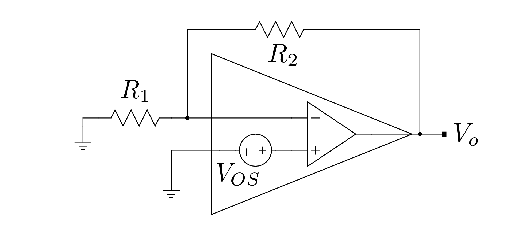
\includegraphics[scale=0.90]{inputOffsetVoltageMeasurement}
\caption{داخلی انحرافی برقی دباو کی پیمائش}
\label{شکل_داخلی_انحرافی_برقی_دباو_کی_پیمائش}
\end{figure}
اس مساوات میں \عددی{V_{OS}} کے علاوہ تمام متغیرات ہمیں معلوم ہیں۔یوں ان سے\عددی{V_{OS}} حاصل کی جا سکتی ہے یعنی
\begin{align}
V_{OS}=\frac{R_1}{R_1+R_2} V_{o}
\end{align}
شکل \حوالہ{شکل_داخلی_انحرافی_برقی_دباو_سے_پاک_منفی_ایمپلیفائر} الف میں اندرونی داخلی انحرافی برقی دباو کے اثر کو ختم کر کے منفی ایمپلیفائر کا استعمال دکھایا گیا ہے۔ایسے ادوار میں \عددی{R_3} اور\عددی{R_5} کی قیمتیں کئی کلو اُوہم  \عددیء{\si{\kilo \ohm}} ہوتی ہیں جبکہ متغیر مزاحمت \عددی{R_4} کی قیمت اتنی رکھی جاتی ہے کہ اس کے درمیانی پنیا سے قابل حصول برقی دباو استعمال کردہ حسابی ایمپلیفائر کے اندرونی داخلی انحرافی برقی دباو \عددی{V_{OS}} کے حدود سے قدر زیادہ ہو۔ایسے متغیر مزاحمت پر پیچ نسب ہوتا ہے جسے گھماتے ہوئے حسابی ایمپلیفائر کے خارجی اشارے \عددی{V_o} کو صفر وولٹ کرتے ہوئے اندرونی داخلی انحرافی برقی دباو کے اثر کو ختم کیا جاتا ہے۔
\begin{figure}
\centering
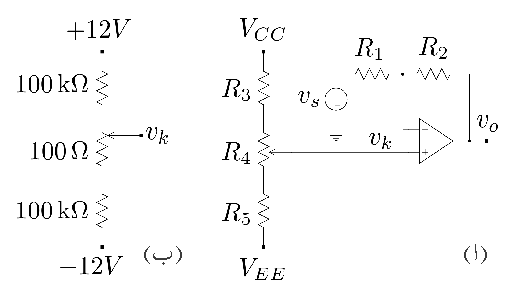
\includegraphics[scale=0.90]{invertingAmplifierWithInputOffsetVoltageEliminated}
\caption{داخلی انحرافی برقی دباو سے پاک، منفی ایمپلیفائر}
\label{شکل_داخلی_انحرافی_برقی_دباو_سے_پاک_منفی_ایمپلیفائر}
\end{figure}

%============================
\ابتدا{مثال}
اگر شکل \حوالہ{شکل_داخلی_انحرافی_برقی_دباو_سے_پاک_منفی_ایمپلیفائر} الف میں
\begin{align*}
V_{CC} =\SI{12}{\volt} \hspace{1cm} V_{EE}=\SI{-12}{\volt} \hspace{1cm} V_{OS}=\SI{2}{\milli \volt}
\end{align*}
ہیں۔داخلی انحرافی برقی دباو کے خاتمے کے لئے درکار مزاحمت \عددیء{R_3}، \عددی{R_4} اور \عددی{R_5} منتخب کریں۔

حل:	چونکہ داخلی انحرافی برقی دباو کی قیمت معلوم ہونے کے باوجود اس کا رخ معلوم نہیں ہوتا لہٰذا ہمیں ان مزاحمت کو یوں منتخب کرنا ہو گا کہ \عددی{R_4} تبدیل کرتے ہوئے ہم \عددی{\SI{-2}{\milli \volt}} تا\عددی{\SI{+2}{\milli \volt}}  یعنی کُل \عددی{\SI{4}{\milli \volt}} کی تبدیلی حاصل کر سکیں۔ہم \عددی{R_3=R_5=\SI{100}{\kilo \ohm}}لیتے ہوئے \عددی{R_4} کی قیمت حاصل کرتے ہیں۔
\begin{align*}
 \left(+12-(-12) \right ) \times \left (\frac{R_4}{R_3+R_4+R_5} \right )&=0.004\\
 24 \times \left ( \frac{R_4}{200000+R_4} \right )&=0.004\\
 R_4 &= \SI{33.34}{\ohm}
\end{align*}
ہم اس سے قدر زیادہ مزاحمت منتخب کرتے ہیں مثلاً \عددی{R_4 =\SI{100}{\ohm}}۔

آئیں دیکھیں کہ ان قیمتوں سے \عددی{v_k} میں کن حدود کے مابین تبدیلی ممکن ہے۔\عددی{R_4} کے متغیر سرے کو ایک جانب پورا گھما کر شکل  الف     میں دکھایا گیا ہے۔اس صورت میں کرخوف کے قانون برائے برقی رو کی مدد سے ہم لکھ سکتے ہیں
\begin{align*}
\frac{v_k-V_{CC}}{R_3}+\frac{v_k-V_{EE}}{R_4+R_5}=0\\
\frac{v_k-12}{100000}+\frac{v_k+12}{100+100000}=0\\
v_k=\SI{5.99}{\milli \volt}
\end{align*}
اسی طرح اگر \عددی{R_4} کو دوسری جانب پورا گھمایا جائے تب
\begin{align*}
\frac{v_k-V_{CC}}{R_3+R_4}+\frac{v_k-V_{EE}}{R_5}=0\\
\frac{v_k-12}{100000+100}+\frac{v_k+12}{100000}=0\\
v_k=-\SI{5.99}{\milli \volt}
\end{align*}
حاصل ہوتا ہے۔موجودہ مثال میں حسابی ایمپلیفائر کا داخلی انحرافی برقی دباو \عددی{\SI{-2}{\milli \volt}} تا\عددی{\SI{+2}{\milli \volt}} کے مابین کہیں پر بھی ہو سکتا ہے۔حسابی ایمپلیفائر کا داخلی اشارہ \عددی{v_s=0} رکھتے ہوئے اس  کے خارجی اشارے \عددی{v_o}  پر نظر رکھ کر \عددی{R_4} کو اس مقام پر لایا جاتا ہے جہاں \عددی{v_o=0} حاصل ہو۔\عددی{R_4} کو اسی قیمت پر پکا چھوڑ دیا جاتا ہے۔
\انتہا{مثال}

شکل \حوالہ{شکل_داخلی_انحرافی_برقی_دباو_سے_پاک_ایمپلیفائر} میں داخلی انحرافی برقی دباو سے پاک منفی اور مثبت ایمپلیفائر دکھائے گئے ہیں۔ان ادوار میں \عددیء{R_3=\SI{100}{\ohm}}، \عددیء{R_4=\SI{150}{\kilo \ohm}}، \عددیء{R_5=\SI{50}{\kilo \ohm}}، \عددی{V_{+}=\SI{12}{\volt}} اور  \عددی{V_{-}=\SI{-12}{\volt}} کی صورت میں \عددی{\SI{\pm 8}{\milli \volt}} کے \اصطلاح{داخلی انحرافی برقی دباو} کا خاتمہ ممکن ہو گا۔ 
\begin{figure}
\centering
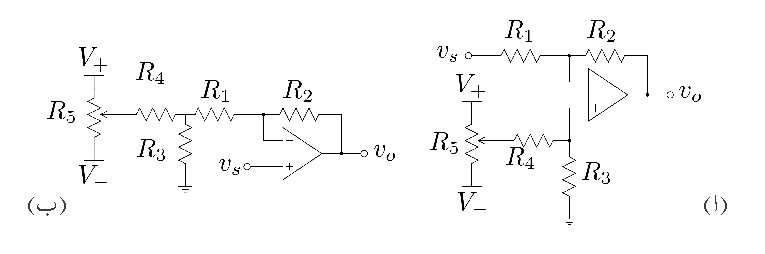
\includegraphics[scale=0.90]{opampInputOffsetVoltageElimination}
\caption{داخلی انحرافی برقی دباو سے پاک ایمپلیفائر}
\label{شکل_داخلی_انحرافی_برقی_دباو_سے_پاک_ایمپلیفائر}
\end{figure}
%=================
\جزوحصہ{داخلی برقی رو کا مسئلہ} \شناخت{حصہ_حسابی_داخلی_برقی_رو}

اگرچہ حسابی ایمپلیفائر کی داخلی برقی رو  \عددی{I_B} کی قیمت عموماً قابل نظر انداز ہوتی ہے البتہ کبھی کبھار نہایت حساس یا باریک اشارات کی قیمت بھی\عددی{I_B} کے لگ بھگ ہوتی ہے۔ایسی صورت میں \عددی{I_B}کو نظر انداز کرنا ممکن نہیں ہوتا۔اس طرح کے مجبوری کے علاوہ بھی ادوار بناتے وقت اگر \عددی{I_B} کو مد نظر رکھا جائے تو کچھ حرج نہیں۔داخلی برقی رو یک سمت نوعیت کا ہوتا ہے۔حسابی ایمپلیفائر کے درست کارکردگی کے لئے یہ ضروری ہے کہ اس کے دونوں داخلی سروں  پر یک سمت برقی رو کے لئے راستہ موجود ہو۔آئیں دیکھتے ہیں کہ اس \عددی{I_B} کے بارے میں عموماً کیا کیا جاتا ہے۔

حسابی ایمپلیفائر کی اندرونی ساخت کی وجہ سے اس کے داخلی سروں پر یک سمت برقی رو درکار ہوتی ہے۔مزید یہ کہ دونوں داخلی سروں پر برقی رو کا رخ ایک ہی سمت میں ہوتا ہے۔اگر کسی ایک قسم کے ایمپلیفائر میں برقی رو کا رخ داخلی سروں پر اندر کی جانب ہو تو کسی دوسرے قسم کے ایمپلیفائر میں دونوں یک سمت داخلی برقی رو کا رخ باہر  کی جانب ہو سکتا ہے۔اس داخلی برقی رو جسے \اصطلاح{داخلی میلان برقی رو}\فرہنگ{داخلی میلان برقی رو}\فرہنگ{input bias current}\حاشیہب{input bias current} کہتے ہیں کے مقدار کا دارومدار ایمپلیفائر کی ساخت پر ہوتا ہے۔
\begin{figure}
\centering
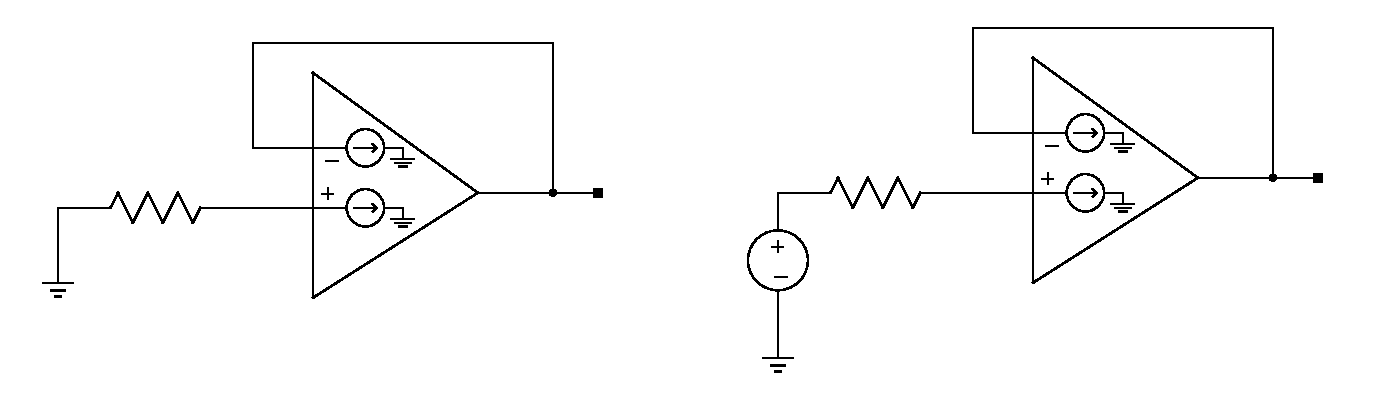
\includegraphics[scale=0.90]{opampInputBiasCurrent}
\caption{داخلی برقی رو کا مسئلہ}
\label{شکل_داخلی_برقی_رو_کا_مسئلہ}
\end{figure}
شکل \حوالہ{شکل_داخلی_برقی_رو_کا_مسئلہ} الف میں مستحکم کار دکھایا گیا ہے جہاں حسابی ایمپلیفائر کے داخلی برقی رو \عددی{I_{B1}} اور\عددی{I_{B2}} کو منبع مستقل برقی رو\حاشیہب{constant current source}  تصور کیا گیا ہے۔یک سمت داخلی اشارہ \عددی{V_S} کی قیمت صفر ہونے کی صورت میں  شکل  الف     حاصل ہوتا  ہے۔مستحکم کار کی خاصیت یہ ہے کہ یہ داخلی اشارہ کو بغیر تبدیلی خارج کرتا ہے۔یوں ہم توقع رکھتے ہیں کہ \عددی{V_S=0} کی صورت میں \عددی{V_O=0} ہو گا مگر ایسا نہیں ہوتا۔شکل  الف     پر غور کرنے سے معلوم ہوتا ہے کہ داخلی برقی رو کی وجہ سے
\begin{align*}
V_K=-I_{B2} R
\end{align*}
حاصل ہوتا ہے۔ \عددی{V_N=V_K} ہونے سے
\begin{align} \label{مساوات_انحرافی_رو_سے_پیدا_دباو}
V_O=-I_{B2}R
\end{align}
حاصل ہو گا۔جیسا کہ پہلے ذکر ہوا، چونکہ عام حالات میں \اصطلاح{داخلی میلان برقی رو} کی قیمت نہایت کم ہوتی ہے لہٰذا اس برقی رو کو عموماً نظر انداز کرنا ممکن ہوتا ہے۔اس وقت ہم کوئی ایسی ترکیب جاننا چاہیں گے کہ نا قابل نظر انداز \اصطلاح{داخلی میلان برقی رو} کی صورت میں یہ دور \عددی{V_O=0}خارج کرے۔

	شکل \حوالہ{شکل_داخلی_برقی_رو_کے_مسئلے_کا_حل} میں مستحکم کار کو ذرا تبدیل کرتے ہوئے اس میں مزاحمت \عددی{R_1} شامل کیا گیا ہے۔مستحکم کار کی کارکردگی ایسا کرنے سے ہرگز متاثر نہیں ہوتی۔اس دور میں بھی
\begin{align*}
V_K=-I_{B2}R
\end{align*}
اور
\begin{align*}
V_N=V_K=-I_{B2}R
\end{align*}
حاصل ہوتا ہے۔البتہ \عددی{R_1} پر اُوہم کے قانون سے
\begin{align*}
V_O-V_N=I_{B1}R_1
\end{align*}
لکھا جا سکتا ہے جس سے
\begin{align*}
V_O=V_N+I_{B1}R_1
\end{align*}
حاصل ہوتا ہے۔اگر دونوں \اصطلاح{داخلی میلان برقی رو} کے قیمتیں برابر ہوں ( \عددی{I_{B1}=I_{B2}=I_B}) تب ہم اس مساوات کو یوں لکھ سکتے ہیں۔
\begin{align*}
V_O=-I_B R +I_B R_1
\end{align*}
دور میں
\begin{align}
R_1=R
\end{align}
لینے سے\عددی{V_O=0} حاصل ہوتا ہے یعنی
\begin{align*}
V_O=-I_B R +I_B R=0
\end{align*}

پس ہم نے دیکھا کہ دور میں دونوں دخول پر یک سمت برقی رو کے لئے برابر مزاحمت نسب کرنے سے \اصطلاح{داخلی میلان برقی رو} کا مسئلہ حل ہو جاتا ہے۔
\begin{figure}
\centering
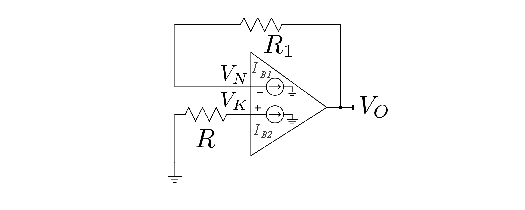
\includegraphics[scale=0.90]{biasCurrentEffectElimination}
\caption{داخلی برقی رو کے مسئلے کا حل}
\label{شکل_داخلی_برقی_رو_کے_مسئلے_کا_حل}
\end{figure}

اگر \عددی{R_1=R}لیتے ہوئے اس حقیقت کو مد نظر رکھا جائے کہ دونوں داخلی برقی رو کے قیمتیں برابر نہیں ہوتیں تو اس صورت میں گزشتہ مساوات سے
\begin{align} \label{مساوات_انحرافی_رو_سے_پیدا_درست_دباو}
V_O=-I_{B2}R+I_{B1}R=\left (I_{B1}-I_{B2} \right )R
\end{align}
حاصل ہوتا ہے۔اگرچہ اس صورت میں \عددی{V_O=0} حاصل نہیں ہو گا مگر چونکہ
\begin{align*}
\abs{I_{B1}-I_{B2}} \ll I_B
\end{align*} 
ہوتا ہے لہٰذا مساوات \حوالہ{مساوات_انحرافی_رو_سے_پیدا_درست_دباو} سے حاصل \عددی{V_O} کی قیمت مساوات \حوالہ{مساوات_انحرافی_رو_سے_پیدا_دباو}  سے حاصل \عددی{V_O} کی قیمت سے زیادہ بہتر (یعنی کم) ہے۔
%=========
\ابتدا{مثال}
منفی ایمپلیفائر میں مسئلہ داخلی برقی دباو کی نشاندہی کریں اور اس سے نپٹنے کا حل دریافت کریں۔

حل:	شکل \حوالہ{شکل_منفی_ایمپلیفائر} میں منفی ایمپلیفائر دکھایا گیا ہے جس میں داخلی اشارہ کی قیمت صفر کرنے سے شکل  \حوالہ{شکل_منفی_ایمپلیفائر_اور_داخلی_برقی_رو_کا_مسئلہ} الف حاصل ہوتا ہے۔
\begin{figure}
\centering
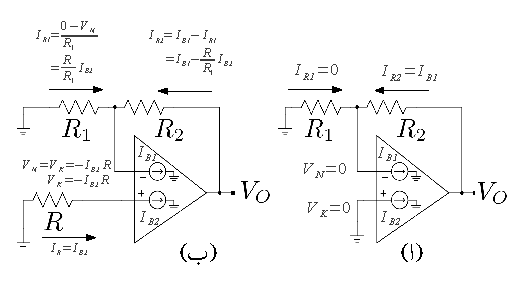
\includegraphics[scale=0.90]{invertingAmplifierWithBiasCurrentEffectEliminated}
\caption{منفی ایمپلیفائر میں مسئلہ داخلی برقی رو اور اس کا حل}
\label{شکل_منفی_ایمپلیفائر_اور_داخلی_برقی_رو_کا_مسئلہ}
\end{figure}
شکل-الف میں مثبت داخلی سرا  برقی زمین کے ساتھ جڑا ہے لہٰذا \عددی{V_K=0} ہے اور یوں \عددی{V_N=V_K=0} ہو گا۔\عددی{V_N=0} ہونے کی وجہ سے\عددی{I_{R1}=0} ہو گا اور یوں منفی داخلی سرے  کی داخلی برقی رو تمام کی تمام مزاحمت \عددی{R_2} سے گزرے گی یعنی \عددی{I_{R2}=I_{B1}}ہو گا۔مزاحمت \عددی{R_2} پر اُوہم کے قانون سے \عددی{V_O} یوں حاصل ہوتا ہے۔
\begin{gather} \label{مساوات_انحرافی_دباو_کا_خاتمہ_ب}
\begin{aligned}
& V_O-V_N=I_{R2}R_2\\
& V_O =V_N +I_{R2}R_2\\
& V_O = 0 +I_{B1}R2\\
& V_O=I_{B1} R_2
\end{aligned}
\end{gather}
شکل \حوالہ{شکل_منفی_ایمپلیفائر_اور_داخلی_برقی_رو_کا_مسئلہ} ب میں مثبت داخلی سرے  سے برقی زمین تک مزاحمت \عددی{R} جوڑ کر داخلی برقی رو کے مسئلے کو حل کرنے کی کوشش کی گئی ہے۔جیسا شکل میں دکھایا گیا ہے \عددی{I_R=I_{B2}} ہونے کی وجہ سے \عددی{V_K=-I_{B2}R} ہو گا۔یوں منفی داخلی سرے  پر بھی اتنا ہی برقی دباو ہو گا (یعنی \عددی{V_N=V_K=-I_{B2}R})۔مزاحمت \عددی{R_1} کا بایاں سرا برقی زمین پر ہے جب کہ اس کا دایاں سرے پر منفی برقی دباو ہے لہٰذا اس میں بائیں سرے سے دائیں سرے کی جانب برقی رو گزرے گا
\begin{align*}
I_{R1}=\frac{R}{R_1}I_{B2}
\end{align*}
 منفی داخلی سرے  پر کرخوف کے قانون برائے برقی رو کی مدد سے \عددی{I_{R2}} یوں حاصل کیا جا سکتا ہے۔
\begin{align*}
&I_{R1}+I_{R2}=I_{B1}\\
&\frac{R}{R_1}I_{B2}+I_{R2}=I_{B1}\\
&I_{R2}=I_{B1}-\frac{R}{R_1}I_{B2}
\end{align*}
مزاحمت \عددی{R_2} پر اُوہم کا قانون استعمال کرتے ہوئے \عددی{V_O} حاصل کرتے ہیں۔
\begin{gather} \label{مساوات_انحرافی_دباو_کا_خاتمہ_الف}
\begin{aligned}
& V_O-V_N=I_{R2}R_2\\
& V_O=V_N+I_{R2}R_2\\
& V_O=-I_{B2}R+\left (I_{B1}-\frac{R}{R_1}I_{B2} \right ) R_2
\end{aligned}
\end{gather}
اگر دونوں داخلی میلان برقی رو کی قیمتیں برابر ہوں یعنی \عددی{I_{B1}=I_{B2}} تب اس مساوات سے حاصل ہوتا ہے۔
\begin{gather}
\begin{aligned}
 V_O&=-I_B R + \left (I_B-\frac{R}{R_1}I_B \right ) R_2\\
&=I_B \left (-R+R_2-\frac{R R_2}{R_1} \right ) 
\end{aligned}
\end{gather}
ہم چاہتے ہیں کہ داخلی میلان برقی رو کی وجہ سے کسی قسم کا خارجی برقی دباو پیدا نہ ہو۔اس مساوات میں\عددی{V_O=0}  استعمال کرتے ہوئے ہم \عددی{R} کی وہ قیمت دریافت کر سکتے ہیں جس سے ایسا ممکن ہو یعنی
\begin{align}
R=\frac{R_1 R_2}{R_1+R_2}
\end{align}
پس منفی ایمپلیفائر کے مثبت داخلی سرے  اور برقی زمین کے درمیان متوازی جڑے \عددی{R_1} اور \عددی{R_2} کے برابر مزاحمت نسب کرنے سے داخلی  میلان برقی رو کا مسئلہ حل ہو جاتا ہے۔

اگر دونوں داخلی میلان برقی رو برابر نہ ہوں تب مساوات \حوالہ{مساوات_انحرافی_دباو_کا_خاتمہ_الف}  میں 
\begin{align*}
R=\frac{R_1 R_2}{R_1+R_2}
\end{align*}
لیتے ہوئے
\begin{align}
V_O=\left (I_{B1}-I_{B2} \right )R_2
\end{align}
حاصل ہوتا ہے۔یوں اس صورت میں اگرچہ داخلی میلان برقی رو کا مسئلہ پوری طرح حل نہیں ہوتا لیکن مساوات \حوالہ{مساوات_انحرافی_دباو_کا_خاتمہ_ب}  کے ساتھ موازنہ کرنے سے (چونکہ \عددی{I_{B1}\gg\abs{I_{B1}-I_{B2}}} ہے ) ہم دیکھتے ہیں کہ \عددی{V_O}  میں خاطر خواہ کمی آتی ہے۔

\انتہا{مثال}

%=================================

ہم دیکھتے ہیں کہ حسابی ایمپلیفائر کے دونوں داخلی سروں پر یک سمت میلان برقی رو کو برقی زمین تک پہنچنے کی خاطر برابر مزاحمت فراہم کرنے سے داخلی برقی رو کا مسئلہ حل ہوتا ہے۔یہاں یک سمت میلان برقی رو کے راستے کی بات کی گئی نہ کہ بدلتے برقی رو کے راستے کی۔اس بات کی وضاحت شکل \حوالہ{شکل_مسئلہ_داخلی_برقی_رو_کے_چند_مثال}    کی مدد سے کرتے ہیں۔یاد رہے کہ کپیسٹر میں یک سمت برقی رو نہیں گزر سکتا اور یہ بالکل لامحدود مزاحمت کی طرح کردار ادا کرتا ہے۔شکل  \حوالہ{شکل_منفی_ایمپلیفائر_اور_داخلی_برقی_رو_کا_مسئلہ} الف میں منفی ایمپلیفائر دکھایا گیا ہے جس کا عمومی طور پر مثبت داخلی سرا برقی زمین کے ساتھ جڑا ہوتا ہے۔منفی داخلی سرے  کے یک سمت میلان  برقی رو کا برقی زمین تک راستہ \عددی{R_2} ہے اور یوں مثبت داخلی سرے  اور برقی زمین کے درمیان \عددی{R=R_2} جوڑ کر داخلی میلان برقی رو کا مسئلہ حل کیا گیا ہے۔شکل \حوالہ{شکل_منفی_ایمپلیفائر_اور_داخلی_برقی_رو_کا_مسئلہ} ب میں مثبت ایمپلیفائر دکھایا گیا ہے۔یہاں اشارہ کو کپیسٹر کے ذریعہ ایمپلیفائر کے ساتھ جوڑا گیا ہے جس سے اس داخلی سرے  کے میلان برقی رو کو برقی زمین تک راستہ میسر نہیں ہو گا اور یوں یہ ایمپلیفائر کام کرنے سے قاصر ہے۔اس کی صحیح کارکردگی کے لئے ضروری ہے کہ اس داخلی سرے  سے برقی زمین تک یک سمت میلان برقی رو کے لئے راستہ موجود ہو۔چونکہ منفی  داخلی سرے  کے یک سمت میلان برقی رو کا برقی زمین تک راستہ \عددی{R_1} اور \عددی{R_2} کے ذریعہ ہے اور یک سمت میلان برقی رو کے نقطہ نظر سے یہ دونوں مزاحمت متوازی جڑے ہیں لہٰذا مثبت  داخلی سرے  اور زمین کے درمیان مزاحمت
\begin{figure}
\centering
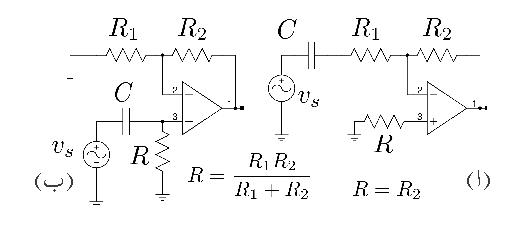
\includegraphics[scale=0.90]{inputBiasCurrentExamplesA}
\caption{مسئلہ داخلی برقی رو کے چند مثالیں اور یک سمت برقی رو کا برقی زمین تک رسائی کا راستہ}
\label{شکل_مسئلہ_داخلی_برقی_رو_کے_چند_مثال}
\end{figure}
%
\begin{align*}
R=\frac{R_1 R_2}{R_1+R_2}
\end{align*}
نسب کر کے اس داخلی سرے  کے یک سمت میلان برقی رو کو زمین تک راستہ فراہم کیا جاتا ہے اور ساتھ ہی ساتھ مسئلہ داخلی میلان برقی رو کو بھی حل کیا جاتا ہے۔یہاں یہ بتلانا ضروری ہے کہ مثبت داخلی سرے  اور زمین کے درمیان مزاحمت \عددی{R} نسب کرنے سے اس داخلی سرے  کا داخلی مزاحمت کم ہوتا ہے جو کہ عموماً قابل برداشت نہیں ہوتا۔



\حصہ{موازنہ کار}
شکل \حوالہ{شکل_حسابی_موازنہ_کار} الف کے حسابی ایمپلیفائر میں \عددی{v_2  > v_1} کی صورت میں \عددی{v_o} مکمل مثبت یعنی \عددی{V_{CC}} پر ہو گا جبکہ \عددی{v_2 < v_1} کی صورت میں \عددی{v_o} مکمل منفی یعنی \عددی{V_{EE}} پر ہو گا۔حسابی ایمپلیفائر داخلی اشارات کا موازنہ کرتے ہوئے \عددی{V_{CC}} یا  \عددی{V_{EE}} خارج کرتا ہے۔یہ عمل نہایت اہم ہے اور اس عمل کی رفتار تیز تر درکار ہوتی ہے۔\اصطلاح{موازنہ کار}\فرہنگ{موازنہ کار}\فرہنگ{comparator}\حاشیہب{comparator} ایسا مخلوط دور ہے جسے خاص اسی مقصد کے لئے تخلیق دیا گیا ہے۔


\begin{figure}
\centering
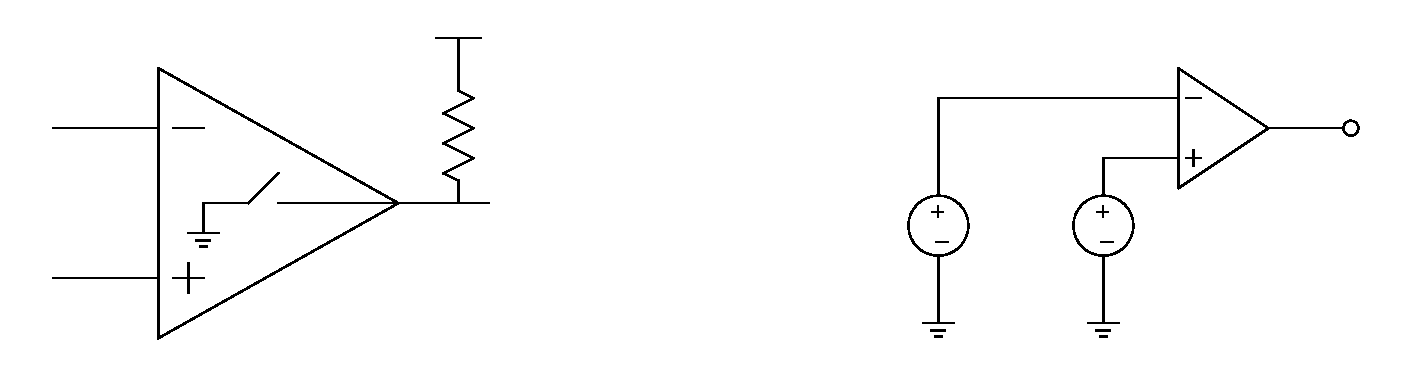
\includegraphics[scale=0.90]{comparator}
\caption{موازنہ کار}
\label{شکل_حسابی_موازنہ_کار}
\end{figure}

\اصطلاح{موازنہ کار} کی علامت وہی ہے جو حسابی ایمپلیفائر کی ہے۔حسابی ایمپلیفائر مثبت یا منفی اشارہ خارج کر سکتا ہے جبکہ  \اصطلاح{موازنہ کار} داخلی اشارات کا موازنہ کرتے ہوئے  دو مختلف صورت اختیار کر سکتا ہے۔ایک صورت میں یہ منقطع ہو جاتا ہے جبکہ دوسری صورت میں یہ مقرر برقی دباو خارج کرتا ہے جو عموماً  \عددی{\SI{0}{\volt}} یا \عددی{V_{EE}} ہوتا ہے۔

\اصطلاح{موازنہ کار}  کی کارکردگی کو شکل  الف     میں دکھایا گیا ہے جہاں اس کے ممکنہ خارجی صورت \اصطلاح{منقطع} اور \عددی{\SI{0}{\volt}} ہیں۔\عددی{v_2 > v_1} کی صورت میں سوئچ منقطع رہتا ہے جبکہ \عددی{v_2 < v_1} کی صورت میں سوئچ چالو ہو کر خارجی سرے  کو برقی زمین کے ساتھ جوڑتا ہے۔خارجی سرے اور \عددی{V_{CC}} کے درمیان مزاحمت \عددی{R_{\textup{اوپر کھینچ}}} جوڑنے سے منقطع صورت میں \عددی{v_o=V_{CC}} حاصل کیا جا سکتا ہے۔

آئیں \اصطلاح{موازنہ کار} کے استعمال کی ایک مثال دیکھیں۔

\ابتدا{مثال}
 اس مثال میں چالو مشین کے درجہ حرارت اور اس میں میکانی دباو پر نظر رکھا جاتا ہے۔اگر ان میں کوئی ایک یا دونوں مقررہ حدف سے تجاوز کریں تو مشین کو منقطع کر دیا جاتا ہے۔مشین اس وقت تک چالو رہتا ہے جب تک اسے چالو رکھنے والا \عددی{\SI{5}{\volt}} کا اشارہ ملتا رہے۔مشین اسی دم منقطع ہو جاتا ہے جب اسے منقطع کرنے والا \عددی{v_o=\SI{0}{\volt}} کا اشارہ ملے۔منقطع کر دینے والے اشارے کو تیر کے نشان سے دکھایا گیا ہے۔

شکل \حوالہ{شکل_حسابی_موازنہ_کار_مقررہ_حدف} میں  دو \اصطلاح{موازنہ کار} متوازی جوڑے گئے ہیں۔نچلے \اصطلاح{موازنہ کار} کے منفی داخلی سرے  پر \تحریر{TMP37}\حاشیہب{Analog Devices اس مخلوط دور کو بناتے ہیں۔} کا خارجی اشارہ جوڑا گیا ہے جسے شکل میں \اصطلاح{درجہ حرارت} کہا گیا ہے۔\تحریر{TMP37} ایسا مخلوط دور ہے جو درجہ حرارت کے راست متناسب برقی دباو خارج کرتا ہے۔\عددی{\SI{0}{\celsius}} پر \عددی{\SI{0}{\volt}} اور \عددی{\SI{100}{\celsius}} پر  یہ \عددی{\SI{1}{\volt}} خارج کرتا ہے۔اس کو \عددی{\SI{5}{\volt}} کی درکار طاقت مہیا کی گئی ہے۔اسی \اصطلاح{موازنہ کار} کے مثبت داخلی سرے  پر قابل تبدیل مزاحمت نسب کی گئی ہے۔قابل تبدیل مزاحمت پر نسب پیچ کو گھماتے ہوئے \اصطلاح{موازنہ کار} کے مثبت داخلی سرے  پر \عددی{\SI{0}{\volt}} تا \عددی{\SI{5}{\volt}} برقی دباو دیا  جا سکتا ہے جسے  شکل میں \اصطلاح{مقررہ درجہ حرارت} کہا گیا ہے۔\اصطلاح{مقررہ درجہ حرارت} کو \عددی{\SI{0.5}{\volt}} پر رکھا گیا ہے۔\عددی{\SI{50}{\celsius}} پر \تحریر{TMP37} اشاریہ پانچ \عددی{\SI{0.5}{\volt}} خارج کرے گا۔

موازنہ کار اس وقت تک منقطع رہے گا جب تک درجہ حرارت \عددی{\SI{50}{\celsius}} سے کم رہے۔جیسے ہی درجہ حرارت اس حدف سے تجاوز کرے، موازنہ کار  \عددی{v_o=\SI{0}{\volt}} خارج کرتے ہوئے مشین کو منقطع کر دیگا۔
\begin{figure}
\centering
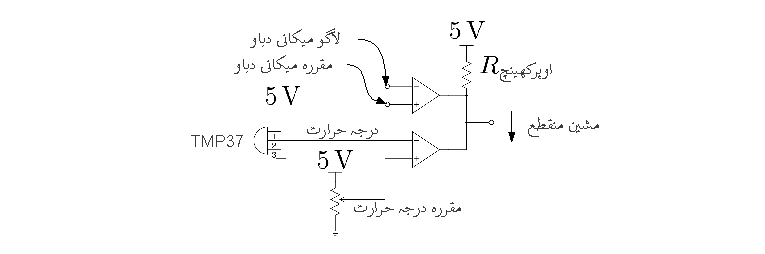
\includegraphics[scale=0.90]{comparatorExample}
\caption{موازنہ کار کی مثال}
\label{شکل_حسابی_موازنہ_کار_مقررہ_حدف}
\end{figure}

شکل میں دکھائے دوسرے موازنہ کار کو بھی اسی طرح استعمال کیا گیا ہے۔اس کا مثبت داخلی سرے کو مقررہ میکانی دباو کے حدف پر رکھا جاتا ہے جبکہ اس کے منفی داخلی سرے  کو مشین میں پائے جانے والے میکانی دباو کا اشارہ مہیا کیا جاتا ہے۔جیسے ہی میکانی دباو مقررہ حدف سے تجاوز  کرے، موازنہ کار خارجی اشارے \عددی{v_o} کو نیچے کھینچ کر برقی زمین \عددی{\SI{0}{\volt}} پر لاتے ہوئے مشین کو منقطع کر دیگا۔

آپ دیکھ سکتے ہیں کہ دونوں موازنہ کار خارجی اشارے کو صرف برقی زمین پر لانے کی صلاحیت رکھتے ہیں۔

اسی طرح مزید موازنہ کار متوازی جوڑتے ہوئے دیگر متغیرات پر نظر رکھی جا سکتی ہے۔
\انتہا{مثال}
%===============================
%=================================
\newpage
\حصہء{سوالات}

\ابتدا{سوال}
شکل \حوالہ{شکل_حسابی_منفی_اقسام} میں
\begin{align*}
V_{CC}=\SI{12}{\volt} \hspace{5mm} V_{EE}=\SI{-12}{\volt} \hspace{5mm} v_s=\SI{0.5}{\volt}\\
R_1=\SI{10}{\kilo \ohm} \hspace {5mm} R_2=\SI{200}{\kilo \ohm} \hspace{5mm} R_3=\SI{10}{\kilo \ohm}
\end{align*}
ہیں۔
\begin{itemize}
\item
کامل حسابی ایمپلیفائر تصور کرتے ہوئے ان تمام ادوار کے داخلی مزاحمت اور خارجی اشارے  حاصل کریں۔
\item
غیر کامل حسابی ایمپلیفائر تصور کرتے ہوئے دوبارہ حل کریں۔غیر کامل حسابی ایمپلیفائر کے جزو
\begin{align*}
A=\num{60000} \hspace{5mm} R_i=\SI{100}{\mega \ohm} \hspace{5mm} R_o=\SI{200}{\ohm}
\end{align*}
ہیں۔
\end{itemize}
%
\begin{figure}
\centering
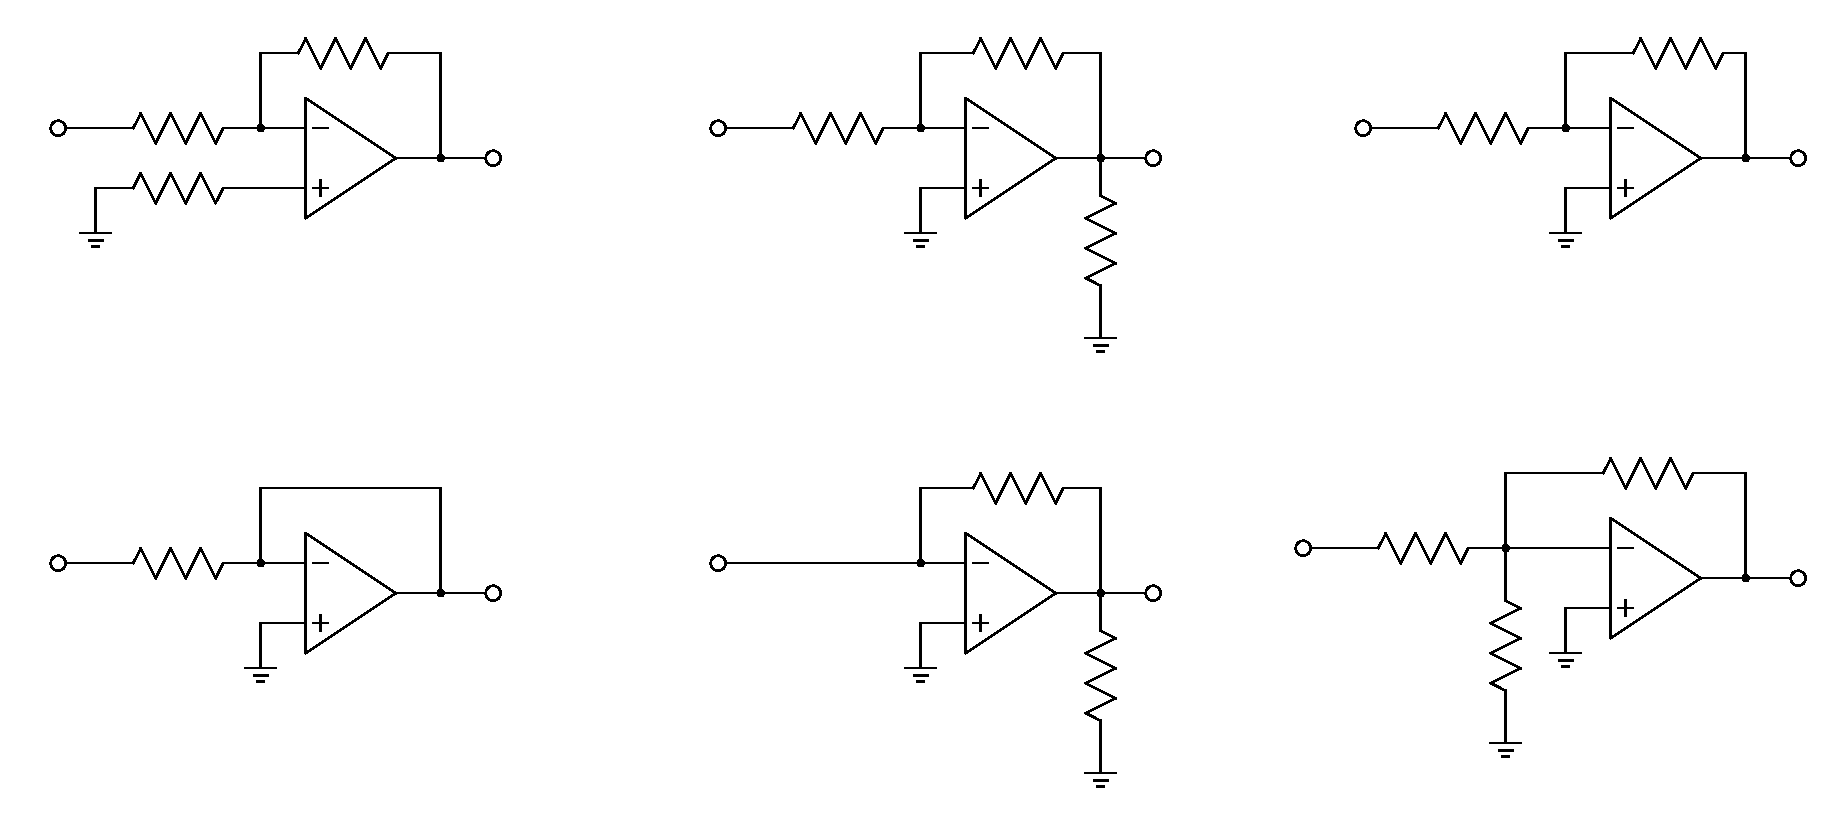
\includegraphics[scale=0.90]{questionsOpampInvertingVariations}
\caption{حسابی منفی ایمپلیفائر کے سوالات}
\label{شکل_حسابی_منفی_اقسام}
\end{figure}

جوابات:
داخلی مزاحمت: \عددیء{\SI{10}{\kilo \ohm}}، \عددیء{\SI{10}{\kilo \ohm}}، \عددیء{\SI{10}{\kilo \ohm}}، \عددیء{\SI{10}{\kilo \ohm}}، \عددیء{\SI{0}{ \ohm}} اور \عددی{\SI{10}{\kilo \ohm}}؛\\
خارجی اشارہ: \عددیء{\SI{-10}{\volt}}، \عددیء{\SI{-10}{\volt}}، \عددیء{\SI{-10}{\volt}}، \عددیء{\SI{-10}{\volt}}، \عددیء{\SI{-12}{\volt}} اور \عددیء{\SI{0}{\volt}}
\انتہا{سوال}
%==================================
\ابتدا{سوال} \شناخت{سوال_سادہ_منفی_ایمپلیفائر}
کامل حسابی ایمپلیفائر تصور کرتے ہوئے \عددی{\SI{10}{\mega \ohm}} سے کم مزاحمتوں کے استعمال سے  صفحہ \حوالہصفحہ{شکل_منفی_ایمپلیفائر} پر دیے شکل \حوالہ{شکل_منفی_ایمپلیفائر} کے طرز پر منفی حسابی ایمپلیفائر تخلیق دیں۔ 
\begin{itemize}
\item
 \عددی{A_v=\SI{-25}{\volt\per \volt}} کی صورت میں \عددی{R_1}، \عددی{R_2} اور زیادہ سے زیادہ ممکنہ داخلی مزاحمت کیا ہو گی۔ 
\item
\عددی{A_v=\SI{-1000}{\volt\per \volt}} کی صورت میں زیادہ سے زیادہ ممکنہ داخلی مزاحمت کیا ہو گی۔ 
\end{itemize}

جوابات: \عددیء{R_1=\SI{400}{\kilo \ohm}}، \عددیء{R_2=\SI{10}{\mega \ohm}}، \عددیء{R_{\textup{داخلی}}=\SI{400}{\kilo \ohm}} اور  \عددیء{R_{\textup{داخلی}}=\SI{10}{\kilo \ohm}}
\انتہا{سوال}
%=====================
\ابتدا{سوال}
\عددی{\SI{200}{\kilo \ohm}} سے کم مزاحمت استعمال کرتے ہوئے  \عددی{A_v=\SI{-1000}{\volt\per \volt}} کا منفی ایمپلیفائر بنانے سے زیادہ سے زیادہ ممکنہ داخلی مزاحمت صرف \عددی{\SI{200}{\ohm}} حاصل ہوتی ہے۔ صفحہ \حوالہصفحہ{شکل_حسابی_منفی_داخلی_زیادہ_مزاحمت} پر دیے شکل \حوالہ{شکل_حسابی_منفی_داخلی_زیادہ_مزاحمت} کے طرز پر ایمپلیفائر بنائیں جس کی داخلی مزاحمت زیادہ سے زیادہ ہو۔

جوابات: \عددیء{R_{\textup{داخلی}}=\SI{200}{\kilo \ohm}}، \عددی{R_1=R_2=\SI{200}{\kilo \ohm}}،  \عددی{\tfrac{R_4}{R_2}+\tfrac{R_4}{R_3}=1000}
\انتہا{سوال}
%=========================
\ابتدا{سوال}
حسابی ایمپلیفائر کی میلان برقی رو حاصل کرنے کی خاطر شکل \حوالہ{شکل__سوال_حسابی_میلان_برقی_رو} استعمال کیا جاتا ہے۔کپیسٹر کے استعمال سے برقی شور کا خاتمہ ہوتا ہے۔
\begin{figure}
\centering
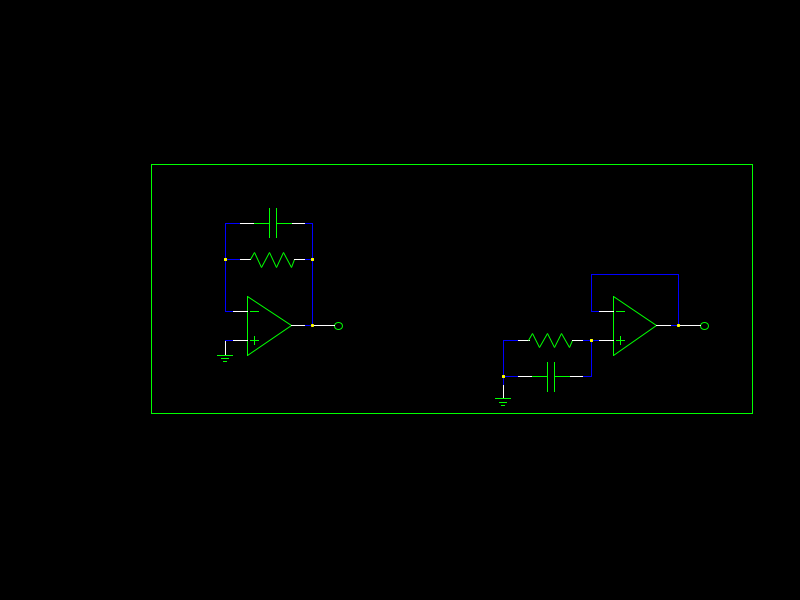
\includegraphics[scale=0.90]{opampInputBiasCurrentMeasurement}
\caption{حسابی ایمپلیفائر کے میلان برقی رو کا حصول}
\label{شکل__سوال_حسابی_میلان_برقی_رو}
\end{figure}
\begin{itemize}
\item
شکل-الف میں \عددی{V_o=\SI{-1.2}{\volt}} جبکہ شکل  الف     میں  \عددی{V_o=\SI{-1.21}{\volt}} پایا جاتا ہے۔مثبت داخلی سرے  کی میلان برقی رو \عددی{I_{B1}} اور منفی داخلی سرے  کی میلان برقی رو \عددی{I_{B2}}  اور ان کی سمتیں حاصل کریں۔
\item
\عددی{I_{B1}} اور \عددی{I_{B1}} سے \اصطلاح{انحرافی  برقی رو} حاصل کریں
\item
ایک حسابی ایمپلیفائر جس کی میلان برقی رو \عددی{\SI{100}{\nano \ampere}} کے لگ بھگ ہے کی مکمل درست میلان برقی رو حاصل کرنے کی خاطر شکل کو استعمال کیا جاتا ہے۔قابل ناپ خارجی اشارہ حاصل کرنے کی خاطر مزاحمت کی وہ قیمت تجویز کریں جس پر \عددی{v_o=\SI{1.5}{\volt}} کے لگ بھگ حاصل ہو۔
\end{itemize}

جوابات: \عددیء{\SI{200}{\nano \ampere}}،\عددی{\SI{201.66}{\nano \ampere}}، داخلی سروں سے باہر جانب، \عددی{\SI{15}{\mega \ohm}}
\انتہا{سوال}
%===============================
\ابتدا{سوال}
عفت بریخنہ نے انجنیئرنگ کے آخری سال میں آلاتی ایمپلیفائر کو استعمال کرتے ہوئے \اصطلاح{برقی قلب نگار}\حاشیہب{ecg} بنانے کا منصوبہ بنایا۔پہلے مرحلے میں انہوں نے شکل \حوالہ{شکل_آلاتی_ایمپلیفائر} میں \عددیء{R_1=\SI{250}{\ohm}}، \عددیء{R_2=\SI{2.5}{\kilo \ohm}} اور \عددی{R_3=R_4=\SI{39}{\kilo\ohm}} رکھ کر دائیں ہاتھ کی کلائی کو \عددی{v_1} جبکہ بائیں ہاتھ کی کلائی کو \عددی{v_2} کے ساتھ جوڑا۔ایسا کرنے کی خاطر \اصطلاح{ہم محوری تار}\فرہنگ{ہم محوری تار}\فرہنگ{تار!ہم محوری}\حاشیہب{co-axial cable} استعمال کئے گئے جن کی بیرونی تامبے کی چادر کو دور کے برقی زمین کے ساتھ جوڑا گیا تا کہ تار میں حساس اشارات پر بیرونی ناپسندیدہ برقی شور کے اثرات کم سے کم کئے جا سکیں۔دایاں ٹخنہ بھی برقی زمین کے ساتھ جوڑا گیا جس سے \عددی{\SI{50}{\hertz}} کا برقی شور نہایت کم ہو جاتا ہے۔حساس اشارات میں واپڈا کے \عددی{\SI{50}{\hertz}} کا شور عموماً پایا جاتا ہے جس سے نپٹنا ضروری ہوتا ہے۔

انہوں نے دیکھا کہ \عددی{v_o} پر دل کی دھڑکن کی چوٹی \عددی{\SI{0.6}{\volt}} تھی۔
\begin{itemize}
\item
اصل اشارہ \عددی{v_2 - v_1} کی قیمت دریافت کریں۔
\item
دل کا کون سا طرف دھڑکتے وقت مثبت برقی دباو پر تھا۔
\end{itemize}
\انتہا{سوال}
%=============

\ابتدا{سوال}
برقی قلب نگار میں برقی شور کے مسئلہ پر تحقیق کرنے کی خاطر عفت نے سائن نما داخلی اشارے کے حیطے کو سو گنا بڑھانے کی خاطر  شکل \حوالہ{شکل_منفی_ایمپلیفائر} میں دکھائے منفی حسابی ایمپلیفائر استعمال کیا جس میں  \عددی{R_1=\SI{1}{\kilo \ohm}} اور \عددی{R_2=\SI{100}{\kilo \ohm}} رکھے گئے۔بغیر زیادہ غور کئے \اصطلاح{لہر بین}\فرہنگ{لہر بین}\حاشیہب{oscilloscope} پر دیکھا گیا کہ \عددی{\SI{0.1}{\volt}} کا اشارہ بڑھاتے وقت دور نہایت عمدگی سے کام کرتے ہوئے \عددی{\SI{10}{\volt}} خارج کرتا ہے۔عفت نے امید رکھی کہ \عددی{\SI{10}{\milli \volt}} کے اشارے کو بھی دور خوش اسلوبی سے بڑھاتے ہوئے \عددی{\SI{1}{\volt}} خارج کرے گا۔\اصطلاح{لہر بین} میں غور سے دیکھتے ہوئے معلوم ہوا ہے کہ خارجی اشارے  کی مثبت چوٹی \عددی{\SI{1.2}{\volt}} جبکہ اس کی منفی چوٹی \عددی{\SI{-0.8}{\volt}} پر تھی۔

\begin{itemize}
\item
\عددی{v_s=\SI{0}{\volt}} کی صورت میں \عددی{v_o} کی کیا قیمت متوقع ہے۔
\item
اگر مسئلہ \اصطلاح{میلان برقی رو} کی وجہ سے پیدا ہوا ہو تب حسابی ایمپلیفائر کے مثبت داخلی سرے  پر  کتنی مزاحمت نسب کرنے سے مسئلہ حل ہو گا۔
\item
مثبت داخلی سرے  پر درکار مزاحمت نسب کرنے سے \عددی{v_s=\SI{0}{\volt}} کی صورت میں \عددی{v_o=\SI{0.19}{\volt}} حاصل ہوتا ہے۔یوں \اصطلاح{میلان برقی رو} کی وجہ سے خارجی اشارے میں \عددی{\SI{10}{\milli \volt}} کا فرق پیدا ہو رہا تھا۔\اصطلاح{میلان برقی رو} کی قیمت حاصل کریں۔
\item 
توقع کی جاتی ہے کہ بقایا \عددی{v_o=\SI{0.19}{\volt}} \اصطلاح{داخلی انحرافی برقی دباو} کی وجہ سے ہے۔استعمال کئے گئے حسابی ایمپلیفائر کی داخلی انحرافی برقی دباو \عددی{V_{OS}} حاصل کریں۔
\end{itemize}

جوابات: \عددیء{\SI{0.2}{\volt}}،  \عددیء{\SI{990}{\ohm}}، \عددیء{I_B=\SI{100}{\nano \ampere}} \عددی{\abs{V_{OS}}=\SI{1.88}{\milli \volt}}
\انتہا{سوال}
%==============================


%==============================
\ابتدا{سوال}
مال لادنے سے پہلے اور لادنے کے بعد ٹرک کا وزن   کرتے ہوئے لدے گئے مال کا وزن حاصل کیا جاتا ہے۔ٹرک کا وزن ناپنے کی خاطر \اصطلاح{لوڈ سیل}\فرہنگ{لوڈ سیل}\حاشیہب{load cell} استعمال کیا جاتا ہے جو در حقیقت \اصطلاح{ویٹ سٹون چکور}\فرہنگ{ویٹ سٹون چکور}\حاشیہب{Wheatstone bridge} پر مشتمل ہوتا ہے۔\اصطلاح{ویٹ سٹون چکور}\حاشیہد{ویٹ سٹون چکور کا نام چارلس ویٹ سٹون سے منسوخ ہے جنہوں نے اس کا استعمال عام بنایا} کو شکل \حوالہ{شکل__سوال_ویٹ_سٹون_چکور} میں دکھایا گیا ہے۔عام صورت میں اس کے چاروں مزاحمتوں کی قیمت برابر \عددی{R} ہوتی ہے۔وزن پڑنے پر ان میں سے ایک مزاحمت کی مزاحمت تبدیل ہو کر \عددی{R+\Delta R} ہو جاتی ہے۔ویٹ سٹون چکور سے اشارات \عددی{V_1} اور \عددی{V_2} حاصل کرتے ہوئے آلاتی ایمپلیفائر کو مہیا کئے جاتے ہیں جو ان میں نہایت باریک فرق \عددی{V_2-V_1} کو بڑھا کر خارج کرتا ہے۔ویٹ سٹون چکور کو آلاتی ایمپلیفائر کے ساتھ جوڑ کر خارجی اشارہ \عددی{v_o} کی مساوات حاصل کریں۔آلاتی ایمپلیفائر کو  صفحہ  \pageref{شکل_آلاتی_ایمپلیفائر} پر شکل \حوالہ{شکل_آلاتی_ایمپلیفائر} میں دکھایا گیا ہے۔

\begin{figure}
\centering

\includegraphics[scale=0.90]{wheatstoneBridge}
\caption{ویٹ سٹون چکور}
\label{شکل__سوال_ویٹ_سٹون_چکور}
\end{figure}

جواب:ویٹ سٹون چکور کا
\begin{align*}
V_2-V_1=\frac{\Delta R}{4 \left(R+\frac{\Delta R}{2} \right)}  V_r
\end{align*}
کے برابر ہے۔اس کو آلاتی ایمپلیفائر کی افزائش سے ضرب دیتے ہوئے
%  
\begin{align*}
v_o=\frac{\Delta R}{4 \left(R+\frac{\Delta R}{2} \right)} \left(\frac{R_4}{R_3}\right) \left(1+\frac{2R_2}{R_1} \right) V_r
\end{align*}
حاصل ہوتا ہے۔

\انتہا{سوال}

%======================
\ابتدا{سوال}
مثبت حسابی ایمپلیفائر میں \عددی{R_1=\SI{1}{\kilo \ohm}} اور \عددی{R_2=\SI{14.7}{\kilo \ohm}} رکھے گئے۔\عددی{v_s=\SI{0.5}{\volt}} اشارے پر \عددی{v_o=\SI{7.85}{\volt}} متوقع ہے۔مزاحمتوں کے قیمتوں میں \عددی{\SI{\pm 5}{\percent}} غلطی  کے گنجائش کی صورت میں
\begin{itemize}
\item
\عددی{v_o}  کے ممکنہ حدود حاصل کریں۔
\item
کل غلطی اصل جواب کے کتنے فی صد ہے۔
\item
اگر کل غلطی کو \عددی{\SI{5}{\percent}} سے کم رکھا جائے تو مزاحمتوں کے قیمت میں زیادہ سے زیادہ کتنے فی صد غلطی قابل برداشت ہو گی۔
\end{itemize}

جوابات: خارجی اشارہ \عددی{\SI{7.15}{\volt}} تا \عددی{\SI{8.62368}{\volt}} ممکن ہے۔   زیادہ سے زیادہ \عددی{v_o} اس وقت حاصل ہو گا جب  \عددی{R_2} کی قیمت \عددی{\SI{5}{\percent}} زیادہ اور \عددی{R_1} کی قیمت  \عددی{\SI{5}{\percent}} کم ہو۔کل غلطی \عددی{\SI{18.77}{\percent}} ہے۔\عددی{\SI{\pm 1.33}{\percent}}

\انتہا{سوال}
%==============
\ابتدا{سوال}
غیر کامل حسابی ایمپلیفائر استعمال کرتے ہوئے  منفی حسابی ایمپلیفائر بنایا جاتا ہے جس میں \عددی{R_1=\SI{5}{\kilo \ohm}} اور \عددی{R_2=\SI{50}{\kilo \ohm}} رکھے جاتے ہیں۔غور کرنے پر معلوم ہوتا ہے کہ \عددی{\tfrac{v_o}{v_s}=\SI{-9.99}{\volt\per \volt}} حاصل ہوا ہے۔کامل حسابی ایمپلیفائر کا مساوی دور استعمال کرتے ہوئے  حسابی ایمپلیفائر کی \عددی{A_d} حاصل کریں۔

جوابات: \عددی{A_d=\SI{10989}{\volt\per \volt}}
\انتہا{سوال}
%====================
\ابتدا{سوال}
صفحہ \حوالہصفحہ{شکل_حسابی_مزاحمت_نما_ایمپلیفائر} پر مزاحمت نما ایمپلیفائر دکھایا گیا ہے۔\عددی{A_d \to \infty} کی صورت میں مزاحمت نما ایمپلیفائر کی
 \عددی{\tfrac{v_o}{i_s}=-R} کے برابر ہوتی ہے۔محدود \عددی{A_d} کی صورت میں  حسابی ایمپلیفائر کے کامل مساوی دور کے استعمال سے \عددی{\tfrac{v_o}{i_s}} اور داخلی مزاحمت حاصل کریں۔

جوابات: \عددی{\tfrac{v_o}{i_s}=-\tfrac{A_d R}{A_d+1}}، \عددی{R_{\textup{داخلی}}=\tfrac{R}{A_d+1}}
\انتہا{سوال}
%=====================================
\ابتدا{سوال}
ایک منفی حسابی ایمپلیفائر جس کی \عددی{A_d=\SI{60000}{\volt\per \volt}} ہو خطی خطے میں رہتے ہوئے \عددی{\SI{12}{\volt}} خارج کر رہا ہے۔کامل مساوی دور استعمال کرتے ہوئے منفی داخلی سرے  پر برقی دباو حاصل کریں۔اگر \عددی{A_d=\SI{1000}{\volt\per \volt}} ہوتا تب جواب کیا ہوتا۔
	
جوابات: \عددیء{\SI{-200}{\micro \volt}}،  \عددیء{\SI{-12}{\milli \volt}} 
\انتہا{سوال}
%===========================
\ابتدا{سوال}
لامحدود \عددی{A_d} کی صورت میں منفی حسابی ایمپلیفائر کی \عددی{A_v=-\tfrac{R_2}{R_1}} حاصل ہوتی ہے۔
\begin{itemize}
\item
محدود  \عددی{A_d} کی صورت میں صفحہ \حوالہصفحہ{شکل_کامل_حسابی_ایمپلیفائر_کا_مساوی_دور} پر شکل \حوالہ{شکل_کامل_حسابی_ایمپلیفائر_کا_مساوی_دور} میں دیے  کامل مساوی دور استعمال کرتے ہوئے \عددی{A_v} حاصل کریں۔ 
\item
لامحدود \عددی{A_d} کے جواب کی نسبت سے \عددی{A_v} میں غلطی کا فی صد حاصل کریں۔
\item
\عددی{A_d=\SI{10000}{\volt\per \volt}} کی صورت میں \عددی{\tfrac{R_2}{R_1}} کی وہ قیمت حاصل کریں جس پر \عددی{A_v} میں غلطی \عددی{\SI{0.1}{\percent}}ہو۔
\item
\عددی{A_d=\SI{10000}{\volt\per \volt}} کی صورت میں \عددی{R_2=\SI{9}{\kilo \ohm}} رکھتے ہوئے \عددی{R_1} کی وہ قیمت حاصل کریں جس پر \عددی{A_v} بالکل برابر \عددی{\SI{-50}{\volt\per \volt}} ہو۔اگر ایمپلیفائر میں \عددی{R_1=\SI{180}{\ohm}} پہلے سے نسب ہو تو \عددی{R_1} کے متوازی کتنی مزاحمت جوڑنے سے  بالکل صحیح درکار \عددی{R_1} حاصل ہوتی ہے۔

\end{itemize}

جوابات: \عددیء{A_v=\tfrac{-A_d R_2}{1+R_1 \left(A_d+1 \right)}}،  \عددیء{100 \left(\tfrac{R_1+R_2}{R_1 A_d +R_2} \right)}، \عددی{\tfrac{R_2}{R_1}=\tfrac{1}{0.111} \approx 9.009}۔آخری جواب سے ظاہر ہے کہ \عددی{A_v =\SI{-9}{\volt\per \volt}} سے زیادہ افزائش پر فرق \عددی{\SI{0.1}{\percent}} سے زیادہ ہو گا۔ \عددی{R_1=\SI{179.9819}{\ohm}}، \عددی{\SI{1.8}{\mega \ohm}}

\انتہا{سوال}
%==============
\ابتدا{سوال}
صفحہ \حوالہصفحہ{شکل_تکمل_کار} پر \اصطلاح{تکمل کار} دکھایا گیا ہے۔اس میں \عددی{R=\SI{14.7}{\kilo \ohm}} اور \عددی{C=\SI{0.01}{\micro \farad}} رکھیں۔حسابی ایمپلیفائر کی داخلی انحرافی برقی دباو \عددی{V_{OS}=\SI{2}{\milli \volt}} ہونے کی وجہ سے خارجی اشارہ صفر وولٹ سے کتنی دیر میں \عددی{V_{CC}=\SI{12}{\volt}} یا \عددی{V_{EE}=\SI{-12}{\volt}} تک پہنچ جائے گا۔اگر \عددی{C=\SI{0.1}{\micro \farad}}  کر دیا جائے تو جواب کیا ہو گا۔

جواب: \عددیء{\SI{0.882}{\second}}،  \عددیء{\SI{8.82}{\second}}۔ ان جوابات سے آپ دیکھ سکتے ہیں کہ داخلی اشارے کی عدم موجودگی یعنی \عددی{v_s=0}  کی صورت میں تکمل کار صفر وولٹ خارج نہیں کرتا بلکہ خارجی اشارہ مکمل مثبت یا مکمل منفی جانب پہنچنے کی کوشش کرتا ہے۔\عددی{RC} کی قیمت بڑھا کر  \عددی{v_o} کی رفتار آہستہ کرتے ہوئے اس عمل کو دیکھنے کی وضاحت دوسری جزو میں کی گئی۔

ایسا بدلتا داخلی اشارہ جس کے مثبت اور منفی حصے  برابر ہوں کے ایک چکر کا اوسط صفر ہوتا ہے۔تکمل کار ایسے اشارے کا تکمل لیتے ہوئے \عددی{V_{OS}} کا بھی تکمل لیتا ہے۔نتیجتاً تکمل کار کا خارجی اشارہ اوسطاً صفر وولٹ پر نہیں رہتا بلکہ اس کی مثبت چوٹی \عددی{V_{CC}} یا منفی چوٹی \عددی{V_{EE}} پر رہتے ہوئے یہ داخلی اشارے کا تکمل لیتا ہے۔

\انتہا{سوال}
%==================
\ابتدا{سوال}
صفحہ \حوالہصفحہ{حصہ_حسابی_عددی_سے_مماثل_کار} پر \اصطلاح{عددی سے مماثل کار} دکھایا گیا ہے۔\عددی{15_{10}} سروں  پر \عددی{\SI{-12}{\volt}} خارج کرنے کی خاطر \عددی{R'} کی قیمت حاصل کریں۔اس صورت \عددی{9_{10}}  پر کتنی مماثل برقی دباو خارج کیا جائے گا۔

جواب:\عددی{15_{10}} در حقیقت \عددی{1111_2} کو ظاہر کرتا ہے۔ \عددی{R'=1.28 R} درکار قیمت ہے۔\عددی{9_{10}} پر \عددی{v_o=\SI{-7.2}{\volt}} خارج کیا جائے گا۔

\انتہا{سوال}
%=======================
\ابتدا{سوال} \شناخت{سوال_حسابی_ٹریکٹر}
چالو ٹریکٹر پر بیٹھے ڈرائیور سے  ٹی وی پر نشریات کی خاطر سوال و جواب کیا جاتا ہے۔ٹریکٹر کی شور کو ختم کرنے کی خاطر دو مائک کا استعمال کیا جاتا ہے۔ایک مائک کو ڈرائیور کے منہ سے دو فٹ کے فاصلے پر جبکہ دوسرے کو منہ کے قریب رکھا جاتا ہے۔دور مائک صرف ٹریکٹر کا شور سنتے ہوئے \عددی{v_{s1}} اشارہ خارج کرتا ہے جبکہ قریب مائک ٹریکٹر کے شور کے ساتھ ساتھ ڈرائیور کی گفتگو بھی حاصل کرتے ہوئے اشارہ \عددی{v_{s2}} خارج کرتا ہے۔ٹریکٹر کے شور کو \عددی{V_t \cos \omega_t t} جبکہ ڈرائیور کے گفتگو کو \عددی{V_d \cos \omega_d t} لکھتے ہوئے
\begin{align*}
v_{s2}=V_t \cos \omega_t t +V_d \cos \omega_d t\\
v_{s1}=V_t \cos \omega_t t
\end{align*} 
اشارات حاصل ہوتے ہیں۔صفحہ \حوالہصفحہ{شکل_منفی_کار} پر دکھائے \اصطلاح{منفی کار} استعمال کرتے ہوئے شور سے پاک اشارہ حاصل کریں۔

جواب: تمام مزاحمت برابر قیمت کے رکھیں۔
\انتہا{سوال}
%==============
\ابتدا{سوال}
سوال \حوالہ{سوال_حسابی_ٹریکٹر} کے سوال و جواب لیتے وقت دیکھا گیا کہ دُور مائک میں نسبتاً زیادہ شور پایا جاتا ہے۔یوں
\begin{align*}
v_{s2}=V_t \cos \omega_t t +V_d \cos \omega_d t\\
v_{s1}=1.2 V_t \cos \omega_t t
\end{align*} 
اشارات حاصل ہوتے ہیں۔حل تجویز کریں۔

جواب: \عددی{\tfrac{R_4 \left(R_1+R_2 \right)}{R_1 \left(R_3+R_4 \right)}=1.2 \tfrac{R_2}{R_1}}
\انتہا{سوال}
%========================
\ابتدا{سوال}
لوہا پگھلانے والی بھٹی تخلیق دیتے وقت معلوم ہوا کہ \عددی{\SI{3}{\kilo \volt}} سے زیادہ برقی دباو پر مسائل پیدا ہوتے تھے۔برقی دباو  کو \عددی{\SI{3}{\kilo \volt}} سے کم رکھنے کی خاطر برقی دباو کا واپسی اشارہ درکار ہے۔واپسی اشارے کو شکل \حوالہ{شکل_سوال_بلند_برقی_دباو_اشارہ} کے منفی ایمپلیفائر میں \عددی{R_2 < R_1} رکھتے ہوئے حاصل کیا جاتا۔\عددی{\SI{3}{\kilo \volt}} پر \عددی{\SI{-6}{\volt}} کا اشارہ درکار ہے۔کسی بھی مزاحمت میں \عددی{\SI{30}{\milli \watt}} سے زیادہ برقی طاقت ضائع نہیں ہونا چاہئے۔ 
\begin{figure}
\centering
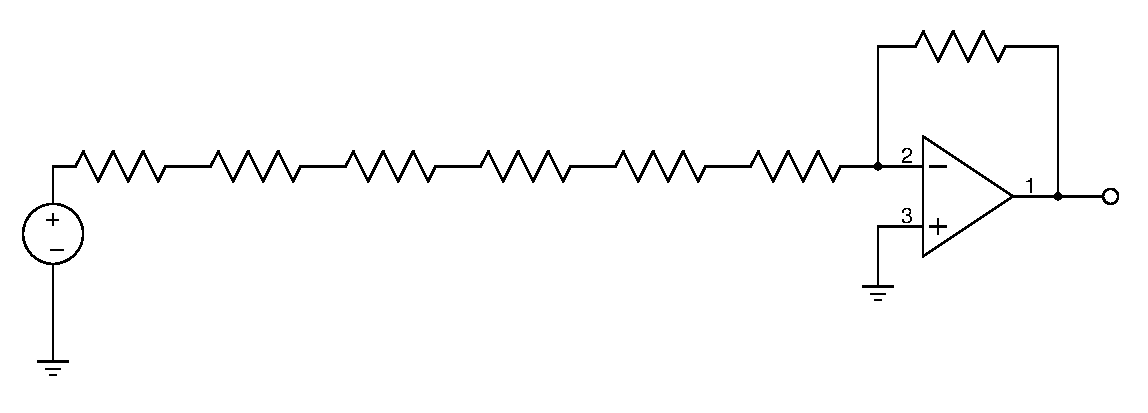
\includegraphics[scale=0.90]{potentialSensor}
\caption{بلند برقی دباو کے اشارے کا حصول}
\label{شکل_سوال_بلند_برقی_دباو_اشارہ}
\end{figure}

جوابات:\عددی{R_1=6R=500 R_2} اور \عددی{R=\SI{8.33}{\mega\ohm}}
\انتہا{سوال}
%=================
\ابتدا{سوال}
\عددیء{R_2=\SI{10}{\kilo\ohm}}، \عددیء{R_1=\SI{2}{\kilo\ohm}}، \عددی{V_{CC}=\SI{12}{\volt}} اور \عددی{V_{EE}=\SI{-12}{\volt}} رکھتے ہوئے منفی حسابی ایمپلیفائر کے داخلی سائن نما اشارے کی زیادہ سے زیادہ چوٹی کیا ہو گی جس پر ایمپلیفائر خطی خطے میں رہتا ہو۔مثبت ایمپلیفائر کے لئے بھی جواب حاصل کریں۔

جوابات: \عددی{\SI{2.4}{\volt}}  اور \عددی{\SI{2}{\volt}} 
\انتہا{سوال}
%================
\ابتدا{سوال}
\اصطلاح{مستطیلی پتلے اشارات}\فرہنگ{مستطیلی پتلا اشارہ}\حاشیہب{pulses} کے \اصطلاح{دورانیہ چڑائی}\فرہنگ{دورانیہ!چڑائی}\حاشیہب{rise time} سے مراد اشارے کا  \عددی{\SI{10}{\percent}} سے  \عددی{\SI{90}{\percent}} چوٹی تک پہنچنے کا دورانیہ ہے۔اسی طرح \اصطلاح{دورانیہ اترائی}\فرہنگ{دورانیہ!اترائی}\حاشیہب{fall time} سے مراد اشارے کا  چوٹی کے \عددی{\SI{90}{\percent}} سے \عددی{\SI{10}{\percent}} تک پہنچنے کا دورانیہ ہے۔

\عددی{\SI{5}{\volt}} چوٹی اور \عددی{\SI{1}{\micro \second}} \اصطلاح{دوری عرصے}\فرہنگ{دوری عرصہ}\حاشیہب{time period} والا \اصطلاح{چکور اشارہ}\حاشیہب{square wave} مستحکم کار کو فراہم کیا جاتا ہے۔دورانیہ چڑائی اور دارانیہ اترائی کا مجموعہ دوری عرصے کے \عددی{\SI{5}{\percent}} سے کم ہونا درکار ہے۔\اصطلاح{رفتار چال} حاصل کریں۔ 

جواب: \عددی{\SI{160}{\volt \per \micro \second}}
\انتہا{سوال}
%====================
\ابتدا{سوال}
صفحہ \حوالہصفحہ{شکل_جمع_و_منفی_کار} پر  \اصطلاح{جمع و منفی کار} دکھایا گیا ہے۔ \اصطلاح{جمع و منفی کار} کے مثبت داخلی سروں  سے جڑے \عددی{v_{j1}} تا \عددی{v_{js}} کو قصر دور کرتے ہوئے مزاحمت \عددی{R_{j1}} تا \عددی{R_{js}} کے داخلی سرے برقی زمین کے ساتھ جوڑتے ہوئے  دور کا خارجی اشارہ \عددی{v_{om}} حاصل کریں۔اسی طرح منفی داخلی سرے  قصر دور کرتے ہوئے خارجی اشارہ \عددی{v_{oj}} حاصل کریں۔تمام داخلی اشارات  کے موجودگی میں خارجی اشارہ \عددی{v_{oj}+v_{om}} کے برابر ہو گا۔اس طرح  مساوات  \حوالہ{مساوات_حسابی_جمع_و_منفی_کار} حاصل کریں۔
\انتہا{سوال}
%=====================
\ابتدا{سوال}
لامحدود \عددی{A_d} کی صورت میں \اصطلاح{مستحکم کار} کا خارجی اشارہ اس کے داخلی اشارے کے برابر ہوتا ہے۔\عددی{A_d=\SI{10000}{\volt \per \volt}} اور
\عددی{A_d=\SI{1000}{\volt \per \volt}} کی صورت میں خارجی اشارہ کتنے فی صد کم  یا زیادہ ہو گا۔

جوابات:خارجی اشارہ  \عددی{\SI{9.999e-3}{\percent}}، \عددی{\SI{0.0999}{\percent}} فی صد کم ہو گا۔
\انتہا{سوال}
%==============
\ابتدا{سوال}
\اصطلاح{منفی کار} اور \اصطلاح{جمع کار} میں تمام مزاحمت برابر ہونے کی صورت میں  \عددی{v_1} کو صفر وولٹ کرتے ہوئے \عددی{v_2} کو نظر آنے والا داخلی مزاحمت کیا ہو گا۔اسی طرح  \عددی{v_2} کو صفر وولٹ کرتے ہوئے \عددی{v_1} کو نظر آنے والا داخلی مزاحمت کیا ہو گا۔جواب بغیر حساب و کتاب کے بتلائیں۔

جوابات:\عددیء{2R}، \عددیء{R}، \عددیء{R}، اور \عددیء{R}
\انتہا{سوال}
%=================
\ابتدا{سوال}\شناخت{سوال_حسابی_مشترکہ_رد_کی_صلاحیت}
صفحہ \حوالہصفحہ{شکل_منفی_کار} پر \اصطلاح{منفی کار} دکھایا گیا ہے۔مساوات \حوالہ{مساوات_حسابی_منفی_کار} اس کی خارجی مساوات ہے۔داخلی اشارات
\begin{align*}
v_{s2}=v_m+\frac{v_f}{2}\\
v_{s2}=v_m-\frac{v_f}{2}
\end{align*}
کے داخلی اشارات منفی کار کو مہیا کئے جاتے ہیں جہاں \عددی{v_m} کو \اصطلاح{مشترکہ اشارہ}\فرہنگ{مشترکہ اشارہ}\حاشیہب{common mode signal} جبکہ \عددی{v_f} کو \اصطلاح{تفرق اشارہ}\فرہنگ{تفرق اشارہ}\حاشیہب{differential mode signal} کہتے ہیں۔خارجی مساوات کو
\begin{align}
v_o=A_{\text{مشترک}} v_m +A_{\text{تفرق}} v_f
\end{align}
صورت میں لکھیں۔مشترکہ افزائش تقسیمِ تفرق افزائش کو \اصطلاح{مشترکہ اشارہ رد کرنے کے صلاحیت}\فرہنگ{مشترکہ اشارہ رد کرنے کے صلاحیت}\حاشیہب{common mode rejection ratio CMRR} \تحریر{CMRR} کہتے ہیں۔ثابت کریں کہ
\begin{align*}
CMRR=\frac{A_{\text{تفرق}}}{A_{\text{مشترک}}}=\frac{1+\frac{1}{2}\left(\frac{R_1}{R_2}+\frac{R_3}{R_4} \right)}{\frac{R_1}{R_2}-\frac{R_3}{R_4}}
\end{align*}
کے برابر ہے۔

\انتہا{سوال}
%===================
\ابتدا{سوال}
منفی کار بناتے وقت \عددی{\tfrac{R_2}{R_1}=\tfrac{R_3}{R_4}} رکھا جاتا ہے جس سے  اس کی \اصطلاح{مشترکہ اشارہ رد کرنے کے صلاحیت} کی قیمت لامحدود حاصل ہوتی ہے۔حقیقی مزاحمتوں کی قیمت ان کے پکارے گئے قیمتوں سے اوپر نیچے ہوتیں ہیں۔سوال \حوالہ{سوال_حسابی_مشترکہ_رد_کی_صلاحیت} میں حاصل جواب کو استعمال کرتے ہوئے ثابت کریں کہ ایسی صورت میں  کم سے کم  \اصطلاح{مشترکہ اشارہ رد کرنے کے صلاحیت} کی قیمت \عددی{\tfrac{A+1+\epsilon^2}{4 \epsilon}} کے برابر ہو گی جہاں \عددی{A=\tfrac{R_2}{R_1}=\tfrac{R_4}{R_3}} کے برابر ہے اور مزاحمت کے قیمتوں میں \عددی{\SI{5}{\percent}} غلطی کے لئے \عددی{\epsilon = 0.05} ہو گا۔

\عددی{R_1=R_3=\SI{1}{\kilo \ohm}} اور \عددی{R_2=R_4=\SI{21}{\kilo \ohm}} کی صورت میں اگر مزاحمتوں کے قیمتوں میں \عددی{\SI{\mp 5}{\percent}}  غلطی کی گنجائش ہو تب  \اصطلاح{مشترکہ اشارہ رد کرنے کے صلاحیت} کی قیمت کیا حاصل ہو گی۔\عددی{\SI{\mp 0.1}{\percent}} کی صورت میں جواب کیا ہو گا۔ 

جوابات: 110،  5500
\انتہا{سوال}
%==================

\ابتدا{سوال}
\عددی{\SI{\mp 12}{\volt}} پر چلنے والے ایک حسابی ایمپلیفائر کا خارجی اشارہ \عددی{\SI{-10.5}{\volt}} تا  \عددی{\SI{+10.5}{\volt}} بغیر بگڑے تبدیل ہو سکتا ہے۔اسے استعمال کرتے ہوئے \عددی{A_v=\SI{-40}{\volt \per \volt}} کا منفی حسابی ایمپلیفائر بنایا جاتا ہے۔داخلی اشارے کی وہ چوٹی \عددی{V_p} حاصل کریں جس پر خارجی اشارہ بگڑ جائے گا۔

جواب: \عددی{\abs{V_p} > \SI{0.2625}{\volt}}
\انتہا{سوال}
%========================


\باب{ڈایوڈ}

الیکٹرانک پرزہ جات میں \اصطلاح {ڈایوڈ}\فرہنگ{ڈایوڈ}\فرہنگ{diode}\حاشیہب{diode}  کلیدی مقام رکھتا ہے۔ڈایوڈ کی علامت شکل \حوالہ{شکل_ڈایوڈ_کی_علامت}  میں دکھائی گئی ہے۔ڈایوڈ کی خاصیت یہ ہے کہ اس کے دو سروں کے مابین، برقی رو صرف ایک رُخ میں گزر سکتی ہے۔ڈایوڈ  کی علامت میں تیر کا نشان اسی رُخ کو ظاہر کرتا ہے۔اس رُخ کو ڈایوڈ کا \اصطلاح {سیدھا رُخ}\فرہنگ{سیدھا رخ}\فرہنگ{رخ!سیدھا}  کہتے ہیں۔ڈایوڈ کے دو اہم اقسام \اصطلاح {سلیکان ڈایوڈ} اور \اصطلاح {جرمینیم ڈایوڈ} ہیں۔سلیکان ڈایوڈ کے خصوصیات جرمینیم ڈایوڈ سے بہت بہتر ہیں۔اسی لئے سلیکان ڈایوڈ زیادہ مقبول ہیں۔اس کتاب میں سلیکان ڈایوڈ پر ہی تبصرہ کیا جائے گا۔  
\begin{figure}
\centering
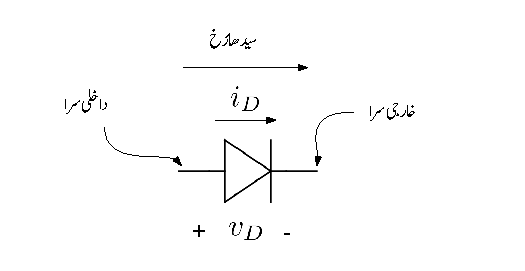
\includegraphics[scale=0.90]{diodeSymbol}
\caption{ڈایوڈ کی علامت}
\label{شکل_ڈایوڈ_کی_علامت}
\end{figure}
ڈایوڈ کے دو سروں کے مابین برقی دباو \عددی{v_D}  اور ڈایوڈ  میں سیدھے رخ  برقی رو \عددی{i_D} کو ناپنے کا درست طریقہ اسی شکل میں دکھایا گیا ہے۔ڈایوڈ کے کارکردگی کی \عددی{v_D-i_D} مساوات مندرجہ ذیل ہے۔
\begin{align}
i_D=I_S \left (e^{\frac{q v_D}{n k T}}-1 \right )
\end{align}
اس مساوات میں \اصطلاح {حرارتی برقی دباو}\فرہنگ{حرارتی!برقی دباو}\فرہنگ{thermal!voltage}\حاشیہب{thermal voltage} \عددی{V_T} کو
\begin{align}
V_T=\frac{k T}{q}
\end{align}
لکھتے ہوئے مساوات کو عموماً یوں لکھا جاتا ہے
\begin{align} \label{مساوات_ڈایوڈ_کی_مکمل_مساوات}
i_D=I_S \left (e^{\frac{v_D}{n V_T}}-1 \right )
\end{align}
جہاں
\begin{description}
\item
[\عددی{I_S}]  \اصطلاح {لبریزی برقی رو}\فرہنگ{لبریزی برقی رو}\فرہنگ{saturation!current}\حاشیہب{saturation current}
\item
[\عددی{q}]  الیکٹران کا \اصطلاح{برقی بار}\فرہنگ{برقی!بار}\فرہنگ{بار}\حاشیہب{charge} \عددی{\SI{1.6e-19}{\coulomb}}
\item
[\عددی{k}]  \اصطلاح {بولٹزمن}\فرہنگ{بالٹزمن کا مستقل}\فرہنگ{Boltzmann constant}\حاشیہب{Boltzmann constant} کا مستقل
  \عددی{\SI{1.38e-23}{\joule / \kelvin}}  
\item
[\عددی{T}]  \اصطلاح {کیلون} پیمائش حرارت\فرہنگ{کیلون پیمائش حرارت}\فرہنگ{Kelvin}\حاشیہب{Kelvin}
\item
[\عددی{V_T}] \اصطلاح {حرارتی برقی دباو}
\item
[\عددی{n}]  \اصطلاح {اخراجی جزو}\فرہنگ{اخراجی جزو}\فرہنگ{emission coefficient}\حاشیہب{emission coefficient} جس کی قیمت ایک تا دو ہوتی ہے۔مخلوط ادوار میں بنائے گئے ڈایوڈ کا عموماً \عددی{n=\num{1}} جبکہ انفرادی دو سروں والے ڈایوڈ کا \عددی{n=\num{2}} ہوتا ہے۔اس کتاب میں \عددی{n=\num{1}} تصور کیا جائے گا۔ 

\end{description}
\عددی{n=\num{1}} لیتے ہوئے
\begin{align} \label{مساوات_ڈایوڈ_کی_مساوات}
i_D=I_S \left (e^{\frac{v_D}{V_T}}-1 \right )
\end{align}
حاصل ہوتا ہے۔اس کتاب میں یہی مساوات بطور ڈایوڈ کی مساوات استعمال کی جائے گی۔

%===========
\ابتدا{مثال}
مندرجہ ذیل حرارت پر حرارتی برقی دباو \عددی{V_T}  کی قیمت حاصل کریں۔
\begin{enumerate}
\item
پانی ابلنے کے درجہ حرارت یعنی \عددی{\SI{100}{\celsius}}  پر\فرہنگ{سیلسیئس}\حاشیہب{Celsius}\فرہنگ{Celsius}

\item

پانی منجمد ہونے کے درجہ حرارت یعنی \عددی{\SI{0}{\celsius}} پر
\item

تئیس ڈگری سیلسیئس یعنی \عددی{\SI{27}{\celsius}}  پر
\end{enumerate}




حل:
\begin{enumerate}
\item
پانی سو ڈگری سیلسیئس یعنی \عددی{\SI{100}{\celsius}} پر اُبلتا ہے۔اس درجہ حرارت جو کہ ڈگری سنٹی گریڈ یا ڈگری سیلسیئس \عددی{\si{\celsius}}  میں ہے کو کیلوین \عددی{\si{\kelvin}} حرارتی پیمائش میں تبدیل کرتے ہیں۔چونکہ \عددی{\si{\kelvin}=\si{\celsius}+\num{273}} ہوتا ہے لہٰذا \عددی{V_T} کی قیمت \عددی{\SI{373}{K}} پر درکار ہے۔یوں 
\begin{align*}
V_T =\frac{k T}{q} =\frac{1.38 \times 10^{-23} \times 373}{1.6 \times 10^{-19}}=\SI{0.03217}{V}
\end{align*}

\item
پانی صفر ڈگری سیلسیئس یعنی \عددی{\SI{273}{\kelvin}} پر منجمد ہوتا ہے۔اس حرارت پر
\begin{align*}
V_T=\frac{k T}{q}=\frac{1.38 \times 10^{-23} \times 273}{1.6 \times 10^{-19}}=\SI{0.0236}{V}
\end{align*}
یعنی \عددی{\SI{23.6}{\milli V}} کے برابر ہے۔
\item
تئیس ڈگری سیلسیئس جسے عام زندگی کا رہائشی درجہ حرارت لیا جاتا ہے پر حرارتی برقی دباو کی قیمت 
\begin{align*}
V_T=\frac{k T}{q}=\frac{1.38 \times 10^{-23} \times 300}{1.6 \times 10^{-19}}=\SI{0.0259}{V}
\end{align*}
یعنی  \عددی{\SI{25.9}{\milli V}} ہے۔
\end{enumerate}
عام طور ڈایوڈ کی مساوات میں حرارتی برقی دباو کو \عددی{\SI{25}{\milli V}} لیا جاتا ہے جسے یاد رکھنا قدرِ آسان ہے یعنی
\begin{align}
V_T=\SI{25}{\milli V}
\end{align}
\انتہا{مثال}
%============

\ابتدا{مثال}
ایک ایسے  ڈایوڈ جس کا \عددی{I_S=\SI{5.1} {\femto A}}  کے برابر ہو کی برقی دباو  \عددی{v_D} ان برقی رو \عددی{i_D} پر حاصل کریں۔
\begin{enumerate}
\item
$i_D=\SI{1}{\milli A}$
\item
$i_D=\SI{10}{\milli A}$
\item
$i_D=\SI{100}{\milli A}$
\end{enumerate}
حل: مساوات \حوالہ{مساوات_ڈایوڈ_کی_مکمل_مساوات}  میں  \عددی{n=1} اور \عددی{V_T=\SI{25}{\milli \volt}} لیتے ہوئے۔
\begin{enumerate}
\item
$v_D=V_T \ln \left (\frac{i_D}{I_S}+1 \right ) =0.025 \times \ln \left (\frac{1 \times 10^{-3}}{5.1 \times 10^{-15}}+1 \right ) =\SI{0.65}{V}$
\item
$v_D=V_T \ln \left (\frac{i_D}{I_S}+1 \right ) =0.025 \times \ln \left (\frac{10 \times 10^{-3}}{5.1 \times 10^{-15}}+1 \right ) =\SI{0.708}{V}$
\item
$v_D=V_T \ln \left (\frac{i_D}{I_S}+1 \right ) =0.025 \times \ln \left (\frac{100 \times 10^{-3}}{5.1 \times 10^{-15}}+1 \right ) =\SI{0.765}{V}$
\end{enumerate}
\انتہا{مثال}
%===========

مثال میں دئے ڈایوڈ سے گزرتے مثبت برقی رو\عددی{i_D}  کی قیمت  سو گنّا بڑھنے سے اس کے برقی دباو \عددی{v_D}  کی قیمت \عددی{\SI{0.65}{\volt} } سے بڑھ کر \عددی{\SI{0.767}{\volt}} ہوئی۔یہ ایک نہایت اہم اور عمومی نتیجہ ہے جسے استعمال کرتے ہم عام طور ایک ایسے سلیکان ڈایوڈ   جس میں سیدھے رُخ برقی رو کا بہاو ہو، کے دو سروں کے مابین برقی دباو کو \عددی{\SI{0.7}{\volt}}  ہی تصور کرتے ہیں یعنی
\begin{align}
v_D=\SI{0.7}{\volt}
\end{align}
یہاں بتلاتا چلوں کہ سیدھے مائل \اصطلاح {جرمینیم ڈایوڈ}\فرہنگ{جرمینیم ڈایوڈ}\فرہنگ{ڈایوڈ!جرمینیم}\حاشیہب{germanium diode}\فرہنگ{diode!germanium} پر \عددی{\SI{0.2}{\volt}} پائے جاتے ہیں۔  

مساوات \حوالہ{مساوات_ڈایوڈ_کی_مکمل_مساوات}  میں \عددی{I_S=\SI{5.1e-15}{\ampere}} لیتے ہوئے اسے مثبت برقی دباو کے لئے  شکل \حوالہ{شکل_ڈایوڈ_کا_خط} میں گراف کیا گیا ہے جہاں افقی محور پر \عددی{v_D} کو وولٹ میں اور عمودی محور پر \عددی{i_D} کو ایمپیئر میں دکھایا گیا ہے۔اس گراف سے واضح ہے کہ \عددی{0.5 V > v_D > 0 V}  کے احاطے میں ڈایوڈ سے گزرتی برقی رو قابلِ نظر انداز ہے۔اگرچہ جب بھی  \عددی{v_D> 0V} ہو ڈایوڈ کو \اصطلاح {سیدھا مائل}\فرہنگ{سیدھا مائل}\فرہنگ{مائل!سیدھا}\فرہنگ{forward biased}\حاشیہب{forward biased} تصور کیا جاتا ہے، حقیقت میں ڈایوڈ کو\عددی{v_D>0.5 V} کی صورت میں ہی \اصطلاح {چالو}\فرہنگ{چالو} تصور کیا جاتا ہے۔یوں \عددی{v_D=0.5 V} کو ڈایوڈ  کی \اصطلاح {چالو برقی دباو}\فرہنگ{چالو برقی دباو}\فرہنگ{برقی دباو!چالو}\فرہنگ{cut-in voltage}\حاشیہب{cut-in voltage}  کہتے ہیں۔چالو ڈایوڈ کی مساوات میں چونکہ 
\begin{align*}
e^{\frac{v_D}{V_T}}>>1
\end{align*}
ہوتا ہے لہٰذا چالو ڈایوڈ کی مساوات یوں لکھی جا سکتی ہے۔
\begin{align} \label{مساوات_چالو_ڈایوڈ}
i_D \approx I_S e^{\frac{v_D}{V_T}}
\end{align}
%
\begin{figure}
\centering
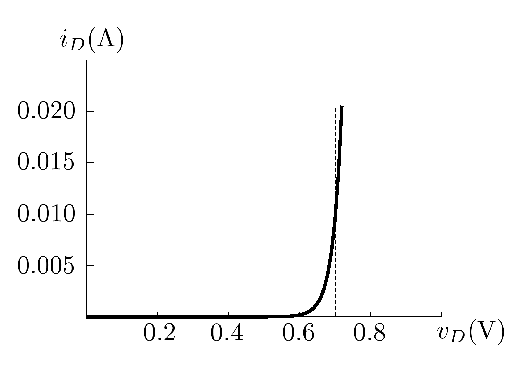
\includegraphics[scale=0.90]{diodeCharacteristics}
\caption{سیدھے مائل ڈایوڈ کا خط}
\label{شکل_ڈایوڈ_کا_خط}
\end{figure} 
شکل \حوالہ{شکل_ڈایوڈ_کا_خط} میں \عددی{\SI{0.7}{\volt}} پر نقطہ دار لکیر لگا کر اس بات کی وضاحت کی گئی ہے کہ سیدھے مائل ڈایوڈ کی برقی دباو \عددی{v_D}  تقریباً \عددی{\SI{0.7}{\volt}} وولٹ رہتی ہے۔ڈایوڈ پر سیدھے رخ برقی دباو کو \اصطلاح {سیدھے رخ ڈایوڈ پر برقی دباو کا گھٹاو}  کہتے ہیں جسے عموماً چھوٹا کر کے سیدھا برقی دباو کا گھٹاو یا مزید چھوٹا کر کے صرف \اصطلاح {سیدھا گھٹاو} کہتے ہیں۔یوں ڈایوڈ کا سیدھا گھٹاو تقریباً\عددی{\SI{0.7}{\volt}} وولٹ تصور کیا جاتا ہے۔

%=========
\ابتدا{مثال}
پچھلے مثال کے  ڈایوڈ کی برقی رو \عددی{i_D}  ان برقی دباو پر حاصل کریں۔
\begin{enumerate}
\item
$v_D=\SI{-10}{\volt}$
\item
$v_D=\SI{-1}{\volt}$
\item
$v_D=\SI{-0.1}{\volt}$
\end{enumerate}

حل:
\begin{enumerate}
\item
$
i_D=I_S \left (e^{\frac{v_D}{V_T}}-1 \right )=I_S \left (e^{-\frac{10}{0.025}} -1\right )=I_S \left(e^{-400}-1 \right ) \approx -I_S
$
\item
$
i_D=I_S \left (e^{\frac{v_D}{V_T}}-1 \right )=I_S \left (e^{-\frac{1}{0.025}} -1\right ) =I_S \left (e^{-40}-1 \right ) \approx -I_S
$
\item
$
i_D=I_S \left (e^{\frac{v_D}{V_T}}-1 \right )=I_S \left (e^{-\frac{0.1}{0.025}}-1 \right ) =I_S \left (e^{-4}-1 \right ) \approx -I_S
$
\end{enumerate}


\انتہا{مثال}
%============
\ابتدا{مثال}\شناخت{مثال_ڈایوڈ_الٹے_مائل_برقی_رو_لبریزی_ہے}
\عددی{I_S} کی قیمت درجہ حرارت بڑھنے سے  \عددی{\SI{15}{\percent}} فی کیلون بڑھتی ہے۔\عددی{\SI{5}{\celsius}} درجہ حرارت بڑھنے سے \عددی{I_S} کی قیمت کتنی ہو جائے گی۔

حل:درجہ حرارت \عددی{\SI{1}{\celsius}} بڑھنے سے نئی قیمت \عددی{1.15 I_S} ہو جائے گی۔مزید \عددی{\SI{1}{\celsius}} بڑھنے سے  \عددی{I_S} مزید \عددی{\SI{15}{\percent}} بڑھ کر \عددی{1.15 \times 1.15 I_S} یعنی \عددی{1.15^2 I_S} ہو جائے گی۔یوں \عددی{\SI{5}{\celsius}} بڑھنے سے
\begin{align*}
1.15^5 I_S \approx 2 I_S
\end{align*} 
ہو جائے گا۔
\انتہا{مثال}
%=========
اس مثال سے ہم دیکھتے ہیں کہ درجہ حرارت \عددی{\SI{5}{\celsius}} بڑھنے سے \عددی{I_S} کی قیمت دگنی ہو جاتی ہے۔اس طرح اگر مثلاً \عددی{\SI{25}{\celsius}} پر \عددی{I_S=\SI{e-15}{\ampere}} ہو تو \عددی{\SI{30}{\celsius}} پر \عددی{I_S=\SI{2e-15}{\ampere}} اور \عددی{\SI{35}{\celsius}} پر \عددی{I_S=\SI{4e-15}{\ampere}} ہو جائے گی۔
%===========
\ابتدا{مشق}
\عددی{\SI{25}{\celsius}} پر \عددی{I_S=\SI{e-15}{\ampere}}  ہے۔ \عددی{\SI{125}{\celsius}} پر \عددی{I_S} کی قیمت حاصل کریں۔

جواب:\عددی{2^{20} \times I_S \approx \SI{1}{\nano \ampere}}
\انتہا{مشق}

آپ نے مثال \حوالہ{مثال_ڈایوڈ_الٹے_مائل_برقی_رو_لبریزی_ہے} میں دیکھا کہ منفی \عددی{v_D} کی صورت میں برقی رو کی قیمت   تقریباً \عددی{-I_S} کے برابر ہوتی ہے یعنی برقی رو کا بہاو ڈایوڈ میں اُلٹی رُخ کی جانب ہوتا ہے جبکہ اس کا کل مقدار \عددی{\abs{I_S}} رہتا ہے۔یاد رہے کہ \عددی{I_S} ایک نہایت چھوٹی مقدار ہے جسے عموماً صفر ہی تصور کیا جاتا ہے۔حقیقی ڈایوڈ میں الٹے رخ برقی رو کی قیمت  \عددی{I_S} سے کئی درجہ زیادہ ہوتی ہے۔مثلاً جہاں الٹے مائل ڈایوڈ کے مساوات کے مطابق \عددی{I_S=\SI{e-15}{\ampere}} برقی رو گزرنا چاہئے وہاں حقیقت میں الٹے رخ \عددی{\SI{e-9}{\ampere}} برقی رو بھی ممکن ہے۔مزید یہ کہ الٹا مائل کرنے والا برقی دباو بھی الٹے رخ برقی رو کی مقدار  پر اثر انداز ہوتا ہے۔

الٹے رخ برقی رو کا بیشتر حصہ ڈایوڈ میں \اصطلاح {الٹے رخ رستا برقی رو}\فرہنگ{الٹی رستا برقی رو}\فرہنگ{برقی رو!الٹی رستا}\فرہنگ{reverse leakage current}\حاشیہب{reverse leakage current}  ہے جو ڈایوڈ کے \عددی{pn} جوڑ کے رقبے کے ساتھ راہ راست تناسب رکھتا ہے۔\عددی{I_S} بھی ڈایوڈ کے \عددی{pn} جوڑ کے رقبے کے ساتھ راہ راست تناسب رکھتا  ہے۔درجہ حرارت \عددی{\SI{5}{\celsius}} بڑھنے سے\عددی{I_S} کی قیمت دگنا ہو جاتی ہے جبکہ  \اصطلاح {الٹے رخ رستا برقی رو} کی قیمت  \عددی{\SI{10}{\celsius}} بڑھنے سے دگنا ہوتی ہے۔


جب ڈایوڈ پر بیرونی لاگو برقی دباو ڈایوڈ میں الٹے رخ برقی رو گزارنے کی کوشش کرے ہم کہتے ہیں کہ ڈایوڈ  \اصطلاح {الٹا مائل}\فرہنگ{مائل!الٹا}\فرہنگ{reverse biased}\حاشیہب{reverse biased}  کیا گیا ہے اور اسی طرح بیرونی لاگو برقی دباو ڈایوڈ میں سیدھے رخ برقی رو گزارنے کی کوشش کرے تب ہم کہتے ہیں کہ ڈایوڈ \اصطلاح {سیدھا مائل}\فرہنگ{سیدھا مائل}\فرہنگ{مائل!سیدھا}\فرہنگ{forward biased}\حاشیہب{forward biased} کیا گیا ہے۔
\begin{figure}
\centering
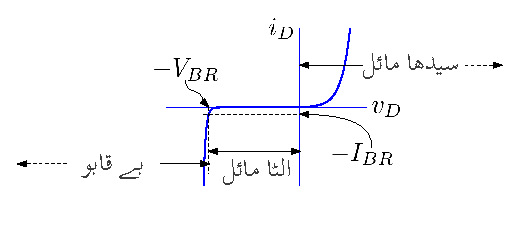
\includegraphics[scale=0.90]{diodeVIcurve}
\caption{ڈایوڈ کا برقی دباو بالمقابل برقی رو کا خط}
\label{شکل_ڈایوڈ_برقی_دباو_بالمقابل_برقی_رو}
\end{figure}
شکل \حوالہ{شکل_ڈایوڈ_برقی_دباو_بالمقابل_برقی_رو}  میں ڈایوڈ کا برقی دباو بالمقابل برقی رو \عددی{(v_D-i_D)} کا خط دکھایا گیا ہے جس میں ڈایوڈ کے سیدھے مائل اور الٹے مائل خطے دکھائے گئے ہیں۔اس شکل میں \اصطلاح {بے قابو خطہ}\فرہنگ{بے قابو خطہ}\فرہنگ{breakdown region}\حاشیہب{breakdown region} بھی دکھایا گیا ہے جو مساوات \حوالہ{مساوات_ڈایوڈ_کی_مکمل_مساوات}  سے کسی صورت اخذ نہیں کیا جا سکتا۔

دراصل مساوات \حوالہ{مساوات_ڈایوڈ_کی_مکمل_مساوات}  حاصل کرتے وقت ڈایوڈ کی کئی پیچیدگیاں نظر انداز کی گئیں اور یوں اگرچہ یہ مساوات سیدھے مائل ڈایوڈ کی کارکردگی کو بہت بہتر بیان کرتا ہے، الٹے مائل ڈایوڈ کی کارکردگی کو یہ پوری طرح صحیح بیان نہیں کرتا اور ڈایوڈ کے بے قابو خطے کو سراسر خطا کر جاتا ہے۔بے قابو خطے پر آگے تبصرہ کیا جائے گا۔یہاں صرف اتنا بتانا ضروری ہے کہ اگر ڈایوڈ پر الٹے رخ برقی دباو لاگو کر کے اسے الٹا مائل کیا جائے تو ڈایوڈ اس برقی دباو کو برداشت کرتا ہے اور الٹے رخ برقی رو نہیں گزرنے دیتا۔اگر اس الٹا مائل کرنے والے برقی دباو کو بتدریج بڑھائی جائے تو آخر کار یہ ڈایوڈ کے برداشت کے حد سے تجاوز کر جائے گا اور ڈایوڈ یک دم الٹے رخ بے قابو برقی رو گزارنے دے گا۔جس برقی دباو پر ایسا ہو اسے ڈایوڈ کی  \اصطلاح {ناقابلِ برداشت الٹ برقی دباو}\فرہنگ{ناقابل برداشت الٹ برقی دباو}\فرہنگ{reverse breakdown voltage}\حاشیہب{reverse breakdown voltage} \عددی{V_{BR}}   کہتے ہیں۔اگرچہ گراف میں ناقابلِ برداشت برقی دباو منفی محور پر ہے، اس کی قیمت مثبت لکھی اور پڑھی جاتی ہے۔مختلف ڈایوڈ کی ناقابل برداشت برقی دباو مختلف ہوتی ہے اور یہ چند وولٹ سے ہزاروں وولٹ تک ممکن ہے۔


شکل \حوالہ{شکل_ڈایوڈ_برقی_دباو_بالمقابل_برقی_رو} میں دکھائے تین خطوں کی نشاندہی یوں کی جاتی ہے۔
\begin{itemize}
\item
سیدھا مائل  \عددی{0 < v_D}
\item
الٹا مائل \عددی{-V_{BR}< v_D < 0}
\item
بے قابو \عددی{v_D < -V_{BR}}
\end{itemize}
ڈایوڈ کی مساوات میں \عددی{V_T} واضح طور پر درجہ حرارت پر منحصر ہے۔اگرچہ\عددی{I_S} کو مستقل سمجھا گیا ہے،حقیقت میں یہ بھی درجہ حرارت پر منحصر ہوتا ہے۔اگر ڈایوڈ میں سیدھے رخ برقی رو کی قیمت تبدیل نہ کرتے ہوئے درجہ حرارت بڑھایا جائے تو مساوات \حوالہ{مساوات_ڈایوڈ_کی_مکمل_مساوات}  میں\عددی{V_T} کی وجہ سے ہم توقع کرتے ہیں کہ ڈایوڈ پر برقی دباو کی قیمت بھی بڑھے گی۔جیسا شکل \حوالہ{شکل_برقی_دباو_بالمقابل_حرارت}  میں دکھایا گیا ہے،حقیقت میں ایسا نہیں ہوتا اور ہم دیکھتے ہیں کہ برقی رو بدلے بغیر،  \عددی{\SI{1}{\celsius}} درجہ حرارت بڑھانے سے ڈایوڈ پر برقی دباو کی قیمت \عددی{\SI{2}{\milli \volt}} گھٹتی ہے۔دراصل درجہ حرارت بڑھانے سے \عددی{I_S} کی قیمت بھی بڑھتی ہے اور \عددی{I_S}  کا اثر\عددی{V_T} کے اثر پر غالب ہے۔مزید یہ کہ حقیقت میں الٹے رخ برقی رو کی مقدار الٹے رخ برقی دباو کی قیمت بڑھانے سے معمولی بڑھتی ہے۔درجہ حرارت کے ساتھ ڈایوڈ پر برقی دباو کی قیمت کی تبدیلی کو برقیاتی \اصطلاح {تھرمامیٹر}\فرہنگ{تھرمامیٹر}\فرہنگ{thermometer}\حاشیہب{thermometer} بنانے میں بروئے کار لایا گیا ہے۔

\begin{figure}
\centering
\includegraphics[scale=0.90]{diodeVoltageVersusTemperature}
\caption{برقی دباو بالمقابل درجہ حرارت}
\label{شکل_برقی_دباو_بالمقابل_حرارت}
\end{figure}

\ابتدا{مثال}
میں نے لاہور میں ٹھوکر نیاز بیگ کے مقام پر واقع \اصطلاح {عطا گروپ آف انڈسٹریز}\حاشیہب{Atta group of industries} میں کام کرتے ہوئے \اصطلاح {قوی برقیات}\حاشیہب{power electronics} کے میدان میں \عددی{\SI{100}{\kilo \watt}} تا \عددی{\SI{1.5}{\mega \watt}} کے  لوہا پگھالنے کی بھٹیاں\حاشیہب{induction furnaces} بنائیں۔ قوی برقیات میں ہزاروں ایمپیئر اور وولٹ کے صلاحیت رکھنے والے ڈایوڈ استعمال کئے جاتے ہیں۔یہ مثال مجھے اُس وقت درپیش مسائل میں سے لیا گیا ہے۔
 
ایک ڈایوڈ میں یکدم \عددی{\SI{1000}{\ampere}} گزارنے سے اس پر شروع میں \عددی{V_D=\SI{0.724}{\volt}} پائے جاتے ہیں جو کچھ دیر میں گھٹتے ہوئے \عددی{\SI{0.708}{\volt}} ہو کر اسی قیمت پر برقرار رہتے ہیں۔
\begin{itemize}
\item
برقی رو گزرنے سے ڈایوڈ کی اندرونی درجہ حرارت میں کتنا اضافہ پیدا ہوا۔
\item
گرم ہونے کے بعد ڈایوڈ میں برقی طاقت کا ضیاع حاصل کریں۔
\item
فی واٹ طاقت کے ضیاع سے درجہ حرارت میں اضافے کو ڈایوڈ کا \اصطلاح {حرارتی مزاحمت}\فرہنگ{حرارتی!مزاحمت}\فرہنگ{thermal!resistance}\حاشیہب{thermal resistance} کہتے ہیں۔ڈایوڈ کا \اصطلاح {حرارتی مزاحمت} حاصل کریں۔
\end{itemize}

حل:
\begin{itemize}
\item
 \عددی{V_D} میں \عددی{0.708-0.724} یعنی \عددی{\SI{-0.016}{\volt}} کی تبدیلی پیدا ہوئی۔چونکہ \عددی{\SI{1}{\celsius}} درجہ حرارت بڑھنے سے \عددی{V_D} میں \عددی{\SI{-2}{\milli \volt}} کی تبدیلی رونما ہوتی ہے لہٰذا ڈایوڈ کے اندرونی درجہ حرارت میں \عددی{\tfrac{0.016}{0.002}} یعنی \عددی{\SI{8}{\celsius}} کا اضافہ پیدا ہوا۔
\item
ڈایوڈ میں برقی طاقت کا ضیاع \عددی{1000 \times 0.708=\SI{708}{\watt}} ہے۔
\item
\اصطلاح {حرارتی مزاحمت} \عددی{\tfrac{8}{708}=\SI{0.011}{\celsius \per \watt}} ہے۔
\end{itemize}
\انتہا{مثال}

\حصہ{کامل ڈایوڈ}  
	ڈایوڈ   سمجھنے کی خاطر ہم کامل ڈایوڈ  کی بات کرتے ہیں۔کامل ڈایوڈ\حاشیہب{ideal diode}  حقیقت میں نہیں پایا جاتا مگر اسے سمجھنا آسان اور اسے سمجھ کر اصل ڈایوڈ   کی کارکردگی سمجھنا زیادہ آسان ہوتا ہے۔

ڈایوڈ   کی کارکردگی دِل کے والو\حاشیہب{valve}  کی مانند ہے۔دِل کا والو خون کو صرف ایک جانب گزرنے دیتا ہے۔اسی طرح ڈایوڈ   برقی رو کو صرف سیدھے رُخ گزرنے دیتا ہے۔شکل \حوالہ{شکل_پانی_کا_والو}  میں پانی کے پائپ پر نسب والو دکھایا گیا ہے جس کی کارکردگی شکل سے ہی واضح ہے۔

\begin{figure}
\centering
\includegraphics[scale=0.90]{diodeAsValve}
\caption{پانی کے پائپ پر نسب والو}
\label{شکل_پانی_کا_والو}
\end{figure}

برقی نقطہ نظر سے کامل ڈایوڈ   کو ایک ایسا خود کار برقی \اصطلاح {سوئچ}\حاشیہب{switch} تصور کیا جا سکتا ہے جو ڈایوڈ میں سے گزرتی برقی رو کی سمت کو دیکھتے ہوئے \اصطلاح {چالو}\فرہنگ{switch ON}  یا منقطع\حاشیہب{switch OFF}  ہو سکے۔ڈایوڈ   میں سیدھے رخ برقی رو اسے چالو کرتی ہے جبکہ اُلٹ رُخ برقی رو اسے منقطع کرتی ہے۔یوں  ڈایوڈ میں اُلٹی رُخ برقی رو کا گزر ممکن نہیں ہوتا۔شکل \حوالہ{شکل_ڈایوڈ_بطور_برقی_سوئچ}  میں ایسا دکھایا گیا ہے۔اس سوئچ کا خط شکل \حوالہ{شکل_ڈایوڈ_سوئچ_کا_خط} میں دکھایا گیا ہے۔اس شکل کا ڈایوڈ کے خط کے ساتھ موازنہ کریں۔اگر  ڈایوڈ کے \عددی{\SI{0.7}{\volt}}  کو نظر انداز کیا جائے تو یہ دونوں خطوط یکساں معلوم ہوتے ہیں

\begin{figure}
\centering
\includegraphics[scale=0.90]{diodeAsSwitch}
\caption{ڈایوڈ بطور برقی سوئچ}
\label{شکل_ڈایوڈ_بطور_برقی_سوئچ}
\end{figure}


\begin{figure}
\centering
\includegraphics[scale=0.90]{diodeSwitchCharacteristics}
\caption{ڈایوڈ سوئچ کا خط}
\label{شکل_ڈایوڈ_سوئچ_کا_خط}
\end{figure}
\حصہ{ڈایوڈ   کے چند ادوار}
	شکل \حوالہ{شکل_ڈایوڈ_سیدھا_مائل_الٹا_مائل}  میں تین ادوار دکھائے گئے ہیں۔شکل  الف میں برقی دباو \عددیء{v_I}، گھڑی کی سمت میں برقی رو \عددی{i} پیدا کرتا ہے جسے تیر کے نشان سے ظاہر کیا گیا ہے۔شکل  ب اور شکل  پ میں مزاحمت کے ساتھ سلسلہ وار ڈایوڈ   بھی نسب کر دئے گئے ہیں۔شکل  ب میں ڈایوڈ   یوں جوڑا گیا ہے کہ برقی رو \عددی{i} کی سمت شکل \حوالہ{شکل_ڈایوڈ_کی_علامت}  میں دکھائے ڈایوڈ کے سیدھے رخ کی جانب ہے جبکہ شکل  پ میں برقی رو\عددی{i} کی سمت ڈایوڈ کی اُلٹ رخ کی جانب ہے۔یوں شکل  ب میں برقی رو \عددی{i} کا گزر ممکن ہے جبکہ شکل  پ میں برقی رو \عددی{i} کا گزر ناممکن ہے۔
\begin{figure}
\centering
\includegraphics[scale=0.90]{diodeForwardReverseBiased}
\caption{سیدھا مائل ڈایوڈ اور الٹا مائل ڈایوڈ}
\label{شکل_ڈایوڈ_سیدھا_مائل_الٹا_مائل}
\end{figure}
شکل  ب میں برقی دباو \عددی{v_I} ڈایوڈ   کو مائل کرتا ہے کہ یہ برقی رو کو سیدھے رُخ گزرنے دے۔ہم کہتے ہیں کہ ڈایوڈ   \اصطلاح {سیدھے رُخ مائل}  کیا گیا ہے یا کہ ڈایوڈ   \اصطلاح {سیدھا مائل}\فرہنگ{سیدھا مائل}\فرہنگ{forward biased}\حاشیہب{forward biased} کیا گیا ہے۔اس کے برعکس شکل  پ میں برقی دباو \عددی{v_I} ڈایوڈ   میں اُلٹے رُخ برقی رو گزارنے کی کوشش کرتا ہے۔اس صورت میں ہم کہتے ہیں کہ ڈایوڈ   \اصطلاح {اُلٹے رُخ مائل}  کیا گیا ہے یا کہ ڈایوڈ   \اصطلاح {اُلٹا مائل}\فرہنگ{الٹا!مائل}\فرہنگ{reverse biased}\حاشیہب{reverse biased} کیا گیا ہے۔ ڈایوڈ کے سیدھے مائل حال کو \اصطلاح {چالو حال} جبکہ اس کے اُلٹ مائل حال کو \اصطلاح {منقطع حال} بھی کہتے ہیں۔ 
	شکل  ب کے لئے کرخوف  کی مساوات برائے برقی دباو لکھتے ہیں۔
\begin{align} \label{مساوات_ڈایوڈ_سیدھا_مائل_مثال_الف}
v_I=v_D+i R
\end{align}


%==========
\ابتدا{مثال}
شکل \حوالہ{شکل_ڈایوڈ_سیدھا_مائل_الٹا_مائل} ب میں مزاحمت کی قیمت \عددی{\SI{1}{\kilo \ohm}} تصور کریں۔ ڈایوڈ کے برقی دباو \عددی{v_D} کو پہلے نظر انداز کرتے ہوئے اور بعد میں اسے\عددی{\SI{0.7}{\volt}}  لیتے ہوئے مندرجہ ذیل صورتوں میں برقی رو حاصل کریں۔
\begin{enumerate}
\item
$v_I=\SI{22.9}{\volt}$
\item
$v_I=\SI{1.2}{\volt}$
\end{enumerate}

حل:	\عددی{v_D} کو نظر انداز کرتے ہوئے مساوات \حوالہ{مساوات_ڈایوڈ_سیدھا_مائل_مثال_الف}  کی مدد سے حل کرتے ہیں۔
\begin{enumerate}
\item
$i=\frac{v_I}{R}=\frac{22.9}{1000}=\SI{22.9}{\milli \ampere}$
\item
$i=\frac{v_I}{R}=\frac{1.2}{1000}=\SI{1.2}{\milli \ampere}$
\end{enumerate}
اب \عددی{v_D=\SI{0.7}{\volt}} لیتے ہوئے دوبارہ حل کرتے ہیں۔
\begin{enumerate}
\item
$i=\frac{v_I-0.7}{R}=\frac{22.9-0.7}{1000}=\SI{22.2}{\milli \ampere}$
\item
$i=\frac{v_I-0.7}{R}=\frac{1.2-0.7}{1000}=\SI{0.5}{\milli \ampere}$
\end{enumerate}

\انتہا{مثال}
%================

اس مثال میں \عددی{v_I=\SI{22.9 }{\volt}} کی صورت میں \عددی{v_D} کے اثر کو شامل کرنے سے حاصل برقی رو \عددی{i}  کی قیمت پر خاطر خواہ اثر نہیں پڑتا جبکہ\عددی{v_I=\SI{1.2}{\volt}} کی صورت میں اس کے شمولیت سے برقی رو کی قیمت آدھے سے بھی کم ہو جاتی ہے۔اس سے ظاہر ہوتا ہے کہ \عددی{v_D} کو ہر جگہ نظرانداز نہیں کیا جا سکتا۔

\حصہ{بدلتا دباو سے یک سمت دباو کا حصول (سمت کاری)}
 
\جزوحصہ{نصف لہر سمت کاری}
	شکل \حوالہ{شکل_نصف_لہر_مثبت_سمت_کار}  میں بدلتا داخلی برقی دباو \عددی{v_i = V_p \sin \omega t}  کے مثبت حصے ڈایوڈ  کو سیدھا مائل کرتے ہیں۔یوں اس دوران
\begin{align*}
v_o = v_i  - v_D \approx V_p \sin \omega t  - 0.7
\end{align*}
ہوتا ہے جہاں سیدھے مائل ڈایوڈ پر برقی دباو کو تقریباً \عددی{\SI{0.7}{\volt}} لیا گیا ہے۔اس کے برعکس \عددی{v_i}  کے منفی حصے ڈایوڈ کو اُلٹا مائل کر کے منقطع کر دیتے ہیں اور یوں اس دوران  \عددی{v_o = \SI{0}{\volt}} ہوتا ہے۔
\begin{figure}
\centering
\includegraphics[scale=0.90]{halfWaveRectifierPositive}
\caption{نصف لہر مثبت سمت کار}
\label{شکل_نصف_لہر_مثبت_سمت_کار}
\end{figure}
شکل \حوالہ{شکل_نصف_لہر_مثبت_سمت_کار} میں  \عددی{v_i} اور \عددی{v_o} بھی گراف کئے گئے ہیں۔آپ دیکھ سکتے ہیں کہ \عددی{v_o}  کی چوٹی \عددی{v_i} کے چوٹی سے تقریباً \عددی{\SI{0.7}{\volt}} کم ہے۔عمومی استعمال میں \عددی{v_i} کی چوٹی کی قیمت \عددی{\SI{0.7}{\volt}} سے گئی گنّا زیادہ ہوتی ہے اور یوں \عددی{v_o} کے چوٹی کو \عددی{v_i} چوٹی کے برابر ہی تصور کیا جاتا ہے۔

اس دور کی مدد سے بدلتا داخلی برقی دباو جو مثبت اور منفی حصوں پر مشتمل ہے سے ایک ایسی خارجی برقی دباو حاصل کی گئی ہے جس میں داخلی برقی دباو کے صرف مثبت حصے موجود ہیں۔ بدلتا برقی دباو سے نصف لہر کی یک سمت برقی دباو کے حصول کو \اصطلاح {نصف لہر سمت کاری}\حاشیہب{half wave rectification}  کہتے ہیں۔یوں شکل \حوالہ{شکل_نصف_لہر_مثبت_سمت_کار} میں دئے دور کو \قریب{\اصطلاح {نصف لہر مثبت سمت کار}}\فرہنگ{نصف لہر!مثبت سمت کار}\فرہنگ{سمت کار!نصف لہر}\فرہنگ{half wave rectifier!positive}\حاشیہب{half wave positive rectifier}  کہتے ہیں۔

نصف سمت کار جسے عام فہم میں \اصطلاح {آدھا ریکٹیفائر}\حاشیہب{half wave rectifier} کہتے ہیں ایک انتہائی اہم دور ہے جسے استعمال کرتے ہوئے کئی ادوار مثلاً  \اصطلاح {منبع برقی دباو}\فرہنگ{برقی دباو منبع}\حاشیہب{voltage source}\فرہنگ{power supply} ، بیٹری چارجر\حاشیہد{موبائل فون رکھنے والے بیٹری چارجر سے بخوبی آگاہ ہوں گے چونکہ بیٹری بھرنے کے لئے ان کی ضرورت پڑتی ہے۔} وغیرہ بنائے جاتے ہیں۔
\begin{figure}
\centering
\includegraphics[scale=0.90]{halfWaveRectifierNegative}
\caption{نصف لہر منفی سمت کار}
\label{شکل_نصف_لہر_منفی_سمت_کار}
\end{figure}
شکل \حوالہ{شکل_نصف_لہر_منفی_سمت_کار} میں ڈایوڈ کو قدرِ مختلف طریقہ سے جوڑا گیا ہے۔اس صورت میں داخلی برقی دباو \عددی{v_i} کے منفی حصے ڈایوڈ کو سیدھا مائل کرتے ہیں جبکہ اس کے مثبت حصے ڈایوڈ کو اُلٹا مائل کرتے ہیں۔یوں خارجی برقی دباو میں داخلی برقی دباو کے صرف منفی حصے موجود ہوتے ہیں۔اس دور کو \قریب{\اصطلاح {نصف لہر منفی سمت کار}}\فرہنگ{نصف لہر!منفی سمت کار}\فرہنگ{half wave rectifier!negative}\حاشیہب{half wave negative rectifier} کہتے ہیں۔
%==============
\ابتدا{مثال}\شناخت{مثال_نصف_لہر_سمتکار_مستطیل_داخلی_دباو}
بوجھ سے لدے مثبت نصف لہر سمت کار کو \عددی{\SI{50}{\hertz}} تعدد \عددی{\SI{\mp15}{\volt}} حیطے کا مستطیل داخلی اشارہ فراہم کیا جاتا ہے جس کے مثبت اور منفی حصے برابر دورانیہ کے ہیں۔بوجھ \عددی{R_L=\SI{100}{\ohm}} جبکہ \عددی{C=\SI{100}{\micro \farad}} ہیں۔خارجی برقی دباو بلدار ہوتا ہے۔اس میں \اصطلاح {بل}\فرہنگ{بل}\فرہنگ{ripple}\حاشیہب{ripple} کی مقدار حاصل کریں۔ڈایوڈ پر برقی دباو کے گھٹنے کو نظر انداز کریں۔خارجی برقی دباو میں \اصطلاح {بل} کو \عددی{\SI{1}{\volt}} سے کم رکھنے کی خاطر درکار کپیسٹر کی قیمت حاصل کریں۔
\begin{figure}
\centering
\includegraphics[scale=0.90]{halfWaveRectifierSquareInput}
\caption{نصف لہر سمت کار کے خارجی برقی دباو میں بل}
\label{شکل_نصف_لہر_سمتکار_بل}
\end{figure}
حل:
شکل \حوالہ{شکل_نصف_لہر_سمتکار_بل} الف میں صورت حال دکھائی گئی ہے جہاں خارجی برقی دباو کا \اصطلاح {بلدار} ہونا واضح ہے۔داخلی برقی دباو منفی ہونے کے صورت میں ڈایوڈ منقطع رہتا ہے۔اس دوران کپیسٹر \عددی{C} برقی طاقت فراہم کرتا ہے۔پچاس تعدد کے اشارے کا \اصطلاح {دوری عرصہ}\حاشیہب{time period} بیس ملی سیکنڈ ہے۔یوں کپیسٹر سے دس ملی سیکنڈ کے لئے بار کی نکاسی ہوتی ہے۔داخلی برقی دباو کے منفی ہونے کے لمحے کو \عددی{t=0} لیتے ہوئے کپیسٹر پر برقی دباو \عددی{v_C} کو یوں لکھا جا سکتا ہے
\begin{align*}
v_C=V_p e^{-\frac{t}{RC}}
\end{align*}
جہاں \عددی{V_p=\SI{15}{\volt}} ہے۔اس مساوات سے دس ملی سیکنڈ بعد \عددی{v_C=\SI{5.5}{\volt}} حاصل ہوتا ہے جس سے
\begin{align*}
V_{\text{بل}}=15-5.5=\SI{9.5}{\volt}
\end{align*}
حاصل ہوتا ہے۔

بل کو \عددی{\SI{1}{\volt}} رکھنے کی خاطر دس ملی سیکنڈ نکاسی کے بعد \عددی{v_C=15-1=14} درکار ہے۔یوں
\begin{align*}
14=15 e^{-\frac{0.01}{100 C}}\\
C=\SI{1449}{\micro \farad}
\end{align*}
حاصل ہوتا ہے۔کپیسٹر، مزاحمت وغیرہ متعین قیمتوں میں دستیاب ہوتے ہیں لہٰذا انہیں قیمتوں میں سے کپیسٹر، مزاحمت وغیرہ چنا ہوتا ہے۔ہم \عددی{\SI{1500}{\micro \farad}} اور \عددی{\SI{25}{\volt}} کا کپیسٹر استعمال کریں گے۔کپیسٹر کے برقی دباو کی صلاحیت درکار برقی دباو کی چوٹی سے زیادہ ہونا لازمی ہے۔ 

آپ نے دیکھا کہ کپیسٹر کی قیمت بڑھانے سے \اصطلاح {بل} میں کمی آتی ہوتی ہے۔یہ حقیقت برقی دباو کے \اصطلاح {منبع}\حاشیہب{voltage supply} میں کام آئے گی۔
\انتہا{مثال}
%=========
\ابتدا{مثال}
شکل \حوالہ{شکل_بیٹری_چارجر}-ا میں نصف لہر مثبت سمت کار کے خارجی جانب مزاحمت کی جگہ  بیٹری نسب کی گئی ہے۔یوں نصف لہر کار بیٹری میں بار بھرتا ہے۔اس دور میں بیٹری کا برقی دباو \عددی{V_B=\SI{12}{\volt}} جبکہ \عددی{R=\SI{100}{\ohm}} اور \عددی{v_i = 15 \sin \omega t} ہے جہاں \عددی{\omega = 100 \pi} کے برابر ہے۔اس بیٹری چارجر کی برقی رو \عددی{i_B} حاصل کر کے گراف کریں۔مزاحمت \عددی{R} برقی رو کی چوٹی کو ڈایوڈ اور بیٹری کے قابلِ برداشت حد سے نیچے رکھتا ہے۔
\begin{figure}
\centering
\includegraphics[scale=0.90]{batteryCharger}
\caption{بیٹری چارجر}
\label{شکل_بیٹری_چارجر}
\end{figure}
حل:	داخلی برقی دباو \عددی{v_i} کی قیمت مسلسل تبدیل ہوتا ہے۔جب تک \عددی{v_i} کی قیمت بیٹری کے برقی دباو یعنی بارہ وولٹ سے کم رہے ڈایوڈ الٹا مائل رہے گا اور اس میں برقی رو نہیں گزرے گی۔جیسے ہی \عددی{v_i} کی قیمت  \عددی{\SI{+12}{\volt}} سے تجاوز کرے ڈایوڈ سیدھا مائل ہو کر برقی رو گزارے گا اور اس دوران \عددی{v_D}  کو نظر انداز کرتے ہوئے مزاحمت پر  اُوہم کے قانون سے ہم لکھ سکتے ہیں۔
\begin{align*}
i_R=i_B=\frac{v_i-V_B}{R}=\frac{15 \sin 100 \pi t -12 }{100}=0.15 \sin  100 \pi t -0.12
\end{align*}

شکل \حوالہ{شکل_بیٹری_چارجر}  - ب میں بیٹری بھرنے والی برقی رو \عددی{i_B} کے علاوہ \عددی{v_i} اور \عددی{V_B} بھی دکھائے گئے ہیں۔برقی دباو اور برقی رو کو ایک ہی جگہ گراف کیا گیا ہے تا کہ وقت \عددی{t} کے ساتھ مختلف متغیرات کے تعلق کی وضاحت ہو سکے۔ جیسا آپ دیکھ سکتے ہیں بیٹری صرف ان اوقات بھری جاتی ہے جب \عددی{v_i > V_B} ہو۔شکل میں نقطہ دار لکیروں سے ایسے ایک دورانیہ کی نشاندہی کی گئی ہے  جب بیٹری بھر رہی ہو۔کی چوٹی \عددی{\SI{30}{\milli \ampere}} ہے جسے  یوں حاصل کیا گیا۔
\begin{align*}
0.15 \sin \frac{\pi}{2}-0.12=0.15-0.12=\SI{0.03}{\ampere}
\end{align*}

\انتہا{مثال}
%===========


\جزوحصہ{مکمل لہر سمت کاری}
شکل \حوالہ{شکل_مکمل_لہر_سمت_کار} میں \اصطلاح {مکمل لہر سمت کار}\فرہنگ{مکمل لہر سمت کار}\فرہنگ{سمت کار!مکمل لہر}\فرہنگ{full wave rectifier}\حاشیہب{full wave rectifier} دکھایا گیا ہے۔اس دور میں چار ڈایوڈ مربع کی شکل میں جوڑے گئے ہیں اور دور کو \عددی{v_i} بطور بدلتا داخلی برقی دباو مہیا کیا گیا ہے۔دور کی کارکردگی سمجھنے کی خاطر شکل \حوالہ{شکل_مکمل_لہر_سمت_کار_کے_خط} الف  پر توجہ رکھیں۔\عددی{v_i} کی قیمت مثبت ہونے کی صورت میں منبع برقی دباو کے مثبت \عددی{(+)}  سرے سے برقی رو باہر کی جانب ہو گی۔چونکہ برقی رو ڈایوڈ میں الٹی جانب نہیں گزر سکتی لہٰذا یہ ڈایوڈ \عددی{D_2} سے گزرے گی جبکہ اس دوران ڈایوڈ \عددی{D_4} منقطع حال رہے گا۔برقی رو \عددی{D_2} سے خارج ہو کر چونکہ \عددی{D_1} میں الٹی جانب نہیں گزر سکتی لہٰذا یہ مزاحمت \عددی{R} میں داخل ہو گی۔

اسی طرح منبع برقی دباو کے منفی سرے سے برقی رو کی راہ معلوم کرنے کی خاطر ہم دیکھتے ہیں کہ منبع برقی دباو کے منفی \عددی{(-)} سرے پر برقی رو اندر کی جانب ہو گی۔یہ برقی رو صرف \عددی{D_3} کے راستے ہی ممکن ہے چونکہ \عددی{D_1} میں الٹی برقی رو کا گزر ناممکن ہے۔
\begin{figure}
\centering
\includegraphics[scale=0.90]{fullWaveRectifier}
\caption{مکمل لہر سمت کار}
\label{شکل_مکمل_لہر_سمت_کار}
\end{figure}
ہم دیکھتے ہیں کہ مثبت برقی دباو کی صورت میں برقی رو ڈایوڈ  \عددی{D_2} اور  \عددی{D_4} سے گزرتی ہے جبکہ ڈایوڈ  \عددی{D_1} اور  \عددی{D_3} منقطع رہتے ہیں۔اس دوران مزاحمت میں برقی رو کی سمت شکل میں دکھائی گئی ہے۔

اب دیکھتے ہیں کہ منبع برقی دباو کے برقی دباو کی قیمت منفی ہونے کی صورت میں کیا ہوتا ہے۔یہ صورتِ حال شکل \حوالہ{شکل_مکمل_لہر_سمت_کار} - ب میں دکھائی گئی ہے۔اس صورت میں برقی رو ڈایوڈ  \عددی{D_1} اور \عددی{D_4} سے گزرے گی جبکہ  \عددی{D_2} اور  \عددی{D_3} منقطع رہیں گے۔برقی رو اب بھی مزاحمت میں گزشتہ سمت میں ہی گزرے گی۔

یوں جیسا شکل \حوالہ{شکل_مکمل_لہر_سمت_کار_کے_خط}  میں دکھایا گیا ہے، بدلتے داخلی دباو \عددی{v_i} کی قیمت مثبت یا منفی ہو، مزاحمت پر ہر وقت برقی دباو \عددی{v_o}مثبت ہی رہتا ہے۔ چونکہ \عددی{v_o} کی سمت تبدیل نہیں ہوتی لہٰذا یہ یک سمت برقی دباو ہے۔
\begin{figure}
\centering
\includegraphics[scale=0.90]{fullWaveRectifierOutputWave}
\caption{مکمل لہر سمت کار کے داخلی اور خارجی خط}
\label{شکل_مکمل_لہر_سمت_کار_کے_خط}
\end{figure}

\حصہ{چوٹی حاصل کار} \شناخت{حصہ_چوٹی_حاصل_کار}
	شکل \حوالہ{شکل_چوٹی_حاصل_کار}  میں \اصطلاح {چوٹی حاصل کار}\فرہنگ{چوٹی حاصل کار}\فرہنگ{peak detector}\حاشیہب{peak detector} دکھایا گیا ہے۔اس دور کو مثبت آدھے لہر سمت کار میں ڈایوڈ   کے خارجی جانب مزاحمت کی جگہ کپیسٹر نسب کر کے حاصل کیا گیا ہے۔
\begin{figure}
\centering
\includegraphics[scale=0.90]{peakDetector}
\caption{چوٹی حاصل کار}
\label{شکل_چوٹی_حاصل_کار}
\end{figure}
ڈایوڈ پر برقی دباو کے \عددی{\SI{0.7}{\volt}} گھٹنے کو نظر انداز کرتے ہوئے چوٹی حاصل کار کی کارکردگی کچھ یوں ہے۔وقت \عددی{t=0}\حاشیہد{\عددی{t_0} وغیرہ کو نقطوں سے ظاہر کیا گیا ہے} پر  \عددی{v_I} چالو کیا جاتا ہے۔لمحہ\عددی{t_0} یعنی \عددی{t=0} پر داخلی برقی دباو \عددی{v_I} اور خارجی برقی دباو \عددی{v_O} دونوں صفر وولٹ کے برابر ہیں۔لمحہ \عددی{t_0} سے لمحہ \عددی{t_1} تک داخلی برقی دباو ڈایوڈ کو الٹ مائل کرتے ہوئے منقطع رکھتا ہے اور یوں اس دوران \عددی{v_O} صفر رہے گا۔\عددی{t_1} سے \عددی{t_2} تک خارجی برقی دباو \عددی{v_O} خوش اسلوبی سے داخلی برقی دباو \عددی{v_I} کی پیروی کرتے ہوئے کپیسٹر کو بھرتا ہے۔اس دوران دور میں برقی رو کی مساوات مندرجہ ذیل ہے۔
\begin{align*}
i=C \frac{dv_O}{dt}
\end{align*}
\عددی{t_2} گزرتے ہی \عددی{v_I} کی قیمت کم ہونا شروع ہو جاتا ہے۔یوں \عددی{t_2} سے \عددی{t_3} تک \عددی{v_I< v_O} رہتا ہے جس کی وجہ سے ڈایوڈ منقطع رہتا ہے۔اس دوران کپیسٹر سے بار کے نکاسی کا کوئی راستہ موجود نہیں ہوتا لہٰذا کپیسٹر پر برقی دباو برقرار رہتا ہے جسے افقی لکیر سے دکھایا گیا ہے۔\عددی{t_3} گزرتے ہی \عددی{v_I} کی قیمت کپیسٹر پر پائے جانے والے برقی دباو سے بڑھ گیا ہے۔یوں ڈایوڈ ایک مرتبہ پھر سیدھا مائل ہوتے ہوئے چالو صورت اختیار کر لیتا ہے۔\عددی{t_3} تا \عددی{t_4} \عددی{v_O} دوبارہ \عددی{v_I} کی پیروی کرتا ہے۔\عددی{t_4} کے بعد کپیسٹر پر برقی دباو تبدیل نہیں ہوتا۔

اس تجزیہ سے واضح ہے کہ یہ دور داخلی اشارہ کی چوٹی حاصل کر کے اس پر برقرار رہتا ہے۔اسی لئے اسے مثبت \اصطلاح {چوٹی حاصل کار}  کہتے ہیں۔اگر اس دور میں ڈایوڈ الٹے رخ لگایا جائے تو خارجی اشارہ \عددی{v_O} منفی چوٹی حاصل کرے  گا اور یوں اس دور کو \اصطلاح {منفی چوٹی حاصل کار} کہا جائے گا۔

\حصہ{حیطہ اتار کار}
مثبت چوٹی حاصل کار میں کپیسٹر کے متوازی مزاحمت جوڑنے سے \اصطلاح {حیطہ اتار کار}\فرہنگ{حیطہ!اتار کار}\فرہنگ{AM demodulator}\حاشیہب{AM demodulator}  حاصل ہوتا ہے جسے شکل \حوالہ{شکل_حیطہ_اتر_کار}  میں دکھایا گیا ہے۔
\begin{figure}
\centering
\includegraphics[scale=0.90]{demodulatorAM}
\caption{حیطہ اتار کار}
\label{شکل_حیطہ_اتر_کار}
\end{figure}
%
\begin{figure}
\centering
\includegraphics[scale=0.90]{AMmodulation}
\caption{حیطہ سوار اشارہ}
\label{شکل_حیطہ_سوار_اشارہ}
\end{figure}
جیسا کہ آپ دیکھ سکتے ہیں چوٹی \عددی{V_p} کے  فوراً بعد داخلی برقی دباو گھٹتا ہے جبکہ خارجی جانب کپیسٹر اسی چوٹی پر رہ جاتا ہے۔اس سے ڈایوڈ الٹا مائل ہو جاتا ہے اور اس میں سے برقی رو کا گزر ناممکن ہو جاتا ہے۔ڈایوڈ کو منقطع تصور کریں تو ہمارے پاس بار سے بھرا شدہ کپیسٹر \عددی{C}  اور اس کے متوازی جڑا مزاحمت \عددی{R} رہ جاتا ہے۔کپیسٹر کا بار اسی مزاحمت کے راستے  خارج ہو کر اس پر برقی دباو گھٹاتا ہے۔ایسا مندرجہ ذیل مساوات کے تحت ہوتا ہے۔
\begin{align} \label{مساوات_حیطہ_اتار_کار_الف}
v_O=V_{p} e^{-\frac{t}{RC}}
\end{align}

اس مساوات میں چوٹی کو \عددی{t=0} تصور کیا گیا ہے۔کپیسٹر سے بار اس لمحہ تک خارج ہوتا ہے جب تک کپیسٹر پر برقی دباو \عددی{v_O}  دور کے داخلی برقی دباو \عددی{v_I}  سے زیادہ رہے۔جیسے ہی \عددی{v_I}کی مقدار ایک مرتبہ پھر \عددی{v_O}کی مقدار سے تجاوز کر جائے، اسی لمحہ ڈایوڈ دوبارہ سیدھا مائل ہو کر کپیسٹر کو دوبارہ بھرنا شروع کر دیتا ہے۔شکل میں باریک لکیر سے داخلی برقی دباو جبکہ موٹی لکیر سے خارجی برقی دباو دکھایا گیا ہے۔\اصطلاح {حیطہ اتار کار} میں \عددی{RC} کو یوں رکھا جاتا ہے کہ  کپیسٹر پر \عددی{v_I} کے چوٹیوں کے برابر برقی دباو رہے جو دراصل \عددی{v_s} ہی ہے۔یوں اصل اشارہ دوبارہ حاصل ہوتا ہے۔

کسی بھی اشارہ یعنی اطلاع  \عددی{v_s} کو ایک جگہ سے دوسری جگہ منتقل کرنے کی خاطر اسے بلند تعدد کے سائن-نما اشارہ \عددی{v_c} کے حیطے پر \اصطلاح {حیطہ سوار کار}\فرہنگ{حیطہ!سوار کار}\فرہنگ{AM modulator}\حاشیہب{AM modulator} کی مدد سے سوار کیا جاتا ہے۔منتقلی کے مقام پر پہنچنے کے بعد \اصطلاح {حیطہ سوار اشارے} سے \اصطلاح {حیطہ اتار کار} کی مدد سے اصل اشارہ یعنی اطلاع \عددی{v_s} کو  دوبارہ حاصل کیا جاتا ہے۔\عددی{v_c} کے حیطے پر سوار کرنے سے مراد \عددی{v_c} کے حیطے کو \عددی{v_s} کے مطابق تبدیل کرنے کو کہتے ہیں۔اشارہ \عددی{v_s}  کو \اصطلاح{سوار موج}\فرہنگ{سوار!موج}\فرہنگ{موج!سوار}\حاشیہب{carrier wave}\فرہنگ{carrier wave} کہتے ہیں جبکہ اس کی تعدد کو \اصطلاح{تعددِ سوار}\فرہنگ{تعدد!سوار}\فرہنگ{سوار!تعدد}\حاشیہب{modulating frequency}\فرہنگ{modulating frequency} کہتے ہیں۔اسی طرح \عددی{v_c} کو \اصطلاح{سواری موج}\فرہنگ{سواری!موج}\فرہنگ{موج!سواری}\حاشیہب{modulating wave}\فرہنگ{modulating wave} کہتے ہیں جبکہ اس کی تعدد کو \اصطلاح{تعددِ سواری}\فرہنگ{تعدد!سواری}\فرہنگ{سواری!تعدد}\حاشیہب{carrier frequency}\فرہنگ{carrier frequency} کہتے ہیں۔

\عددی{v_s=0.5 \cos \omega_s t} کو مثال بناتے ہوئے آگے بڑھتے ہیں۔حیطہ سوار اشارہ حاصل کرنے کی خاطر \عددی{v_s} اور \عددی{v_c} کو \اصطلاح {حیطہ سوار کار} سے گزارا جاتا ہے جس سے 
\begin{align}\label{مساوات_ڈایوڈ_حیطہ_سوار_اشارہ}
v_I=\left(1+0.5 \cos \omega_s t \right) \cos \omega_c t=V_p \cos \omega t
\end{align}
حاصل ہوتا ہے۔اس اشارہ جس کو شکل \حوالہ{شکل_حیطہ_سوار_اشارہ} میں دکھایا گیا ہے کو \اصطلاح {حیطہ سوار اشارہ}\فرہنگ{حیطہ!سوار اشارہ}\حاشیہب{AM signal}\فرہنگ{AM signal} \عددی{v_I} کہتے ہیں۔

\عددی{v_I} کے دو متواتر چوٹیوں کے درمیان حیطہ اتار کار کے  کپیسٹر پر برقی دباو گھٹتا ہے۔یہ وقفہ تقریباً \عددی{\tfrac{1}{f_c}} کے برابر ہے جسے استعمال کرتے ہوئے  مساوات \حوالہ{مساوات_حیطہ_اتار_کار_الف} سے \اصطلاح {مسئلہ مکلارن} کی مدد سے وقفے کے آخر میں برقی دباو
\begin{align}
v_O=V_{p} e^{-\frac{1}{RC f_c}} \approx V_p \left(1-\frac{1}{RC f_c} +\cdots \right )
\end{align}
حاصل ہوتا ہے۔یوں اس دوران برقی دباو میں تبدیلی
\begin{align*}
\abs{\Delta v_O} =\frac{V_p}{RC f_c}
\end{align*}
حاصل ہوتی ہے یعنی اس وقفے کے دوران خارجی اشارے کی وقت کے ساتھ شرح تبدیلی 
\begin{align}\label{مساوات_ڈایوڈ_حیطہ_اتار_کار_خارجی_اشارہ}
\frac{\abs{\Delta v_O}}{\frac{1}{f_c}} =\frac{V_p}{RC}
\end{align}
ہے۔حیطہ اتار کار میں \عددی{RC} کو یوں رکھا جاتا ہے کہ  بھیجے گئے اشارے \عددی{v_s} میں زیادہ سے زیادہ تبدیلی کو بھی پکڑا جا سکے۔\عددی{v_s} میں تبدیلی کی شرح
\begin{align*}
\od{v_s}{t}=-0.5 \omega_s \sin \omega_s t
\end{align*}
ہے جس کی زیادہ سے زیادہ قیمت \عددی{\omega_s t=\tfrac{n \pi}{2}} پر حاصل ہوتی ہے جہاں \عددیء{n=1,3,5,\cdots} ہے۔یہ قیمت 
\begin{align*}
\abs{\od{v_s}{t}}=0.5 \omega_s 
\end{align*} 
ہے۔اس زیادہ سے زیادہ داخلی اشارے کے تبدیلی کی شرح کو \اصطلاح {حیطہ اتار کار} کے تبدیلی کے شرح کے برابر رکھا جاتا ہے۔\عددی{\omega_s t=\tfrac{n \pi}{2}} پر مساوات \حوالہ{مساوات_ڈایوڈ_حیطہ_سوار_اشارہ} کے تحت \عددی{V_p=1} حاصل ہوتا ہے جسے مساوات \حوالہ{مساوات_ڈایوڈ_حیطہ_اتار_کار_خارجی_اشارہ} میں استعمال کرتے ہوئے یوں
\begin{align}
\frac{1}{RC}=0.5 \omega_s
\end{align}
رکھا جاتا ہے۔یہ مساوات \اصطلاح {حیطہ اتار کار} کی مساوات ہے۔اگر کپیسٹر کو اس مساوات سے حاصل قیمت سے زیادہ رکھا جائے تب خارجی اشارہ تیزی سے تبدیل ہونے والے داخلی اشارے کو نہیں پکڑ سکے گا۔اگر کپیسٹر کی قیمت اس سے کم رکھی جائے تب خارجی اشارے میں \اصطلاح {بل}\فرہنگ{بل}\حاشیہب{ripple} زیادہ پایا جائے گا۔ 

\حصہ{منبع برقی دباو}
سمت کار کے خارجی جانب زیادہ قیمت کا کپیسٹر نسب کر کے \اصطلاح {منبع برقی دباو}\فرہنگ{منبع برقی دباو}\فرہنگ{برقی دباو منبع}\حاشیہب{power supply}  حاصل ہوتا ہے جیسا شکل \حوالہ{شکل_پاور_منبع} الف میں دکھایا گیا ہے۔اس پر کپیسٹر کے متوازی برقی بوجھ لادا جاتا ہے جسے عموماً \عددی{R_L} سے ظاہر کیا جاتا ہے۔\اصطلاح {منبع برقی دباو} یعنی برقی طاقت کے \اصطلاح {منبع} کو  گھریلو بجلی یا صنعتی بجلی فراہم کرتے ہوئے یک سمت برقی دباو \عددی{V_{\text{یکسمتی}}} حاصل کیا جاتا ہے۔
 
بے بوجھ منبع برقی دباو کی کارکردگی بالکل چوٹی حاصل کار کی طرح ہے جبکہ برقی بوجھ سے لدے منبع برقی دباو کی کارکردگی حیطہ اتار کار کی طرح ہے۔البتہ منبع میں ہماری کوشش ہوتی ہے کہ  \عددی{V_{\text{یکسمتی}}} میں \اصطلاح {بل} کم سے کم ہو تا کہ اسے یک سمت برقی دباو کے طور استعمال کرنا ممکن ہو۔منبع برقی دباو تقریباً ہر برقیاتی آلہ یا مشین میں پایا جاتا ہے۔

چونکہ منبع برقی دباو داخلی طاقت \عددی{\SI{50}{\hertz}} کے سائن نما \عددی{v_i} سے حاصل کرتا ہے لہٰذا \عددی{C} بھی اسی تعدد سے بھرتا ہے۔\عددی{v_i} کے دو چوٹیوں کے مابین \عددی{\tfrac{1}{50}=\SI{20}{\milli \second}}  (بیس ملی سیکنڈ )  کے وقفے  کے دوران \عددی{R_L} کو کپیسٹر \عددی{C} طاقت مہیا کرتا ہے۔
\begin{figure}
\centering
\includegraphics[scale=0.90]{powerSupply}
\caption{منبع برقی دباو}
\label{شکل_پاور_منبع}
\end{figure}
\ابتدا{مثال} \شناخت{مثال_پیداکار_برقی_دباو}
ایک عدد \عددی{\SI{12}{\volt}} کا منبع برقی دباو درکار ہے جس سے \عددی{\SI{6}{\kilo \ohm}} داخلی مزاحمت کے برقی بوجھ کو طاقت مہیا کرنا ہے۔برقی بوجھ کو دی جانے والے برقی دباو کے قیمت میں کل تبدیلی \عددی{\SI{\mp 0.5}{\volt}} سے کم ہونا ضروری ہے۔کپیسٹر \عددی{C} کی قیمت حاصل کریں۔

حل: 
شکل \حوالہ{شکل_مثال_پاور_منبع} میں ان معلومات کو دکھایا گیا ہے۔کپیسٹر \عددی{t_1} دورانیہ کے لئے  برقی بوجھ کو طاقت فراہم کرتا ہے اور یوں اس دوران اس سے بار کی نکاسی ہوتی ہے۔البتہ \عددی{t_1} کو دو چوٹیوں کے درمیان وقفے کے برابر ہی عموماً تصور کیا جاتا ہے۔یوں \عددی{t_1=\SI{20}{\milli \second}} لیا جاتا ہے۔

اس مسئلے کو دو طریقوں سے حل کرتے ہیں۔پہلے مثال \حوالہ{مثال_نصف_لہر_سمتکار_مستطیل_داخلی_دباو} کی طرح حل کرتے ہیں۔کپیسٹر نکاسی  کا دورانیہ بیس ملی سیکنڈ ہے۔اس دورانیہ میں  کپیسٹر پر  برقی دباو \عددی{\SI{12.5}{\volt}} سے گھٹ کر \عددی{\SI{11.5}{\volt}} رہ جاتا ہے یوں
\begin{align*}
11.5=12.5 e^{-\frac{0.02}{6000C}}\\
C=\SI{39.98}{\micro \farad}
\end{align*}
حاصل ہوتا ہے۔آئیں اسی مسئلے کو قدر مختلف اور زیادہ آسان طریقے سے حل کریں۔
% 
 \begin{figure}
\centering
\includegraphics[scale=0.90]{powerSupplyA}
\caption{مثال منبع برقی دباو}
\label{شکل_مثال_پاور_منبع}
\end{figure}

درکار بارہ وولٹ کو شکل \حوالہ{شکل_مثال_پاور_منبع} میں پختہ لکیر سے دکھایا گیا ہے۔برقی دباو اس سے \عددی{\SI{0.5}{\volt}} کم یا زیادہ ہو سکتا ہے۔یوں برقی بوجھ میں \اصطلاح {بل}\فرہنگ{بل}\حاشیہب{ripple}\فرہنگ{ripple} \عددی{\SI{0.5}{\volt}} یا \عددی{\SI{1}{\volt}} کے برابر ہے جبکہ زیادہ سے زیادہ برقی دباو \عددی{\SI{12.5}{\volt}} اور کم سے کم برقی دباو \عددی{\SI{11.5}{\volt}} ہے۔بارہ وولٹ پر \عددی{R_L} میں \عددی{\tfrac{12}{6000}=\SI{2}{\milli \ampere}} جبکہ زیادہ سے زیادہ برقی دباو پر  \عددی{\tfrac{12.5}{6000}=\SI{2.08333}{\milli \ampere}} اور کم سے کم برقی دباو پر  \عددی{\tfrac{11.5}{6000}=\SI{1.9167}{\milli \ampere}} کا برقی رو گزرے گا۔

برقی دباو کے تبدیلی سے برقی رو کے تبدیلی کو نظر انداز کرتے ہوئے اس کی اوسط قیمت لی جاتی ہے۔یوں ہم تصور کرتے ہیں کہ \عددی{R_L} میں \عددی{\SI{2}{\milli \ampere}} گزرتا ہے جس سے کپیسٹر کے بار کی نکاسی ہوتی ہے۔ہم جانتے ہیں کہ
\begin{align*}
I=\frac{\Delta Q}{\Delta t}
\end{align*}
کے برابر ہوتا ہے۔ اس سے کپیسٹر میں  \عددی{t_1} کے دوران کپیسٹر پر پائے جانے والے بار میں تبدیلی \عددی{\Delta Q} حاصل کرتے ہیں۔
\begin{align*}
\Delta Q=I \times \Delta t=\left(2 \times 10^{-3} \right) \times \left(20 \times 10^{-3} \right)=40 \times 10^{-6}
\end{align*}
کپیسٹر کی مساوات \عددی{Q=CV} کو \عددی{\Delta Q=C \Delta V} لکھتے ہیں جہاں \عددی{\Delta V=\SI{1}{\volt}} کے برابر ہے۔یوں
\begin{align*}
\Delta Q=I \times \Delta t=C \Delta V
\end{align*}
لکھا جا سکتا ہے جس سے
\begin{align*}
C \times 1&=40 \times 10^{-6}\\
C&=\SI{40}{\micro \farad}
\end{align*}
حاصل ہوتا ہے۔

آپ نے دیکھا کہ دونوں طریقوں سے حل کرتے تقریباً برابر جوابات حاصل ہوتے ہیں۔البتہ دوسرا طریقہ استعمال کرتے ہوئے صرف کاغذ اور قلم استعمال کرتے ہوئے جواب کا حصول ممکن ہے۔
\انتہا{مثال}
%===============

کپیسٹر کی قیمت بڑھانے سے منبع کے خارجی برقی دباو میں \اصطلاح {بل} کم کیا جا سکتا ہے۔حقیقت میں ڈایوڈ میں برقی دباو کا گھٹاو اور داخلی بدلتے برقی دباو میں تبدیلی ہمارے قابو میں نہیں ہوتے لہٰذا اس طرح کی منبع برقی دباو سے قطعی یک سمت برقی دباو کا حصول ممکن نہیں ہوتا۔جہاں درکار یک سمت برقی دباو کی  قیمت چند وولٹ زیادہ یا کم  قابل برداشت ہو وہاں اس طرح کی منبع استعمال کی جا سکتی ہے۔یک سمت برقی دباو کی قیمت زیادہ یا کم ہونے کے باوجود برقی دباو میں \اصطلاح {بل}\فرہنگ{بل}\حاشیہب{ripple}\فرہنگ{ripple} کو کپیسٹر سے قابو رکھنا ممکن ہے۔


%================
\ابتدا{مشق}
\عددی{\SI{10}{\milli \ampere}} کے برقی بوجھ کو چلانے کی خاطر \عددی{\SI{5}{\volt}} کی منبع برقی دباو درکار ہے جس میں \اصطلاح {بل} \عددی{\SI{\mp 0.1}{\volt}} سے کم ہونا ضروری ہے۔کپیسٹر کی قیمت حاصل کریں۔اس قسم کی \اصطلاح {منبع برقی دباو}\فرہنگ{منبع دباو}\حاشیہب{voltage source}\فرہنگ{voltage source} برقیاتی ادوار کو چلانے کی خاطر عموماً درکار ہوتی ہے۔

جواب: \عددی{\SI{1000}{\micro \farad}}
\انتہا{مشق}
%================
مندرجہ بالا مثال کو مد نظر رکھتے ہوئے ہم دیکھتے ہیں کہ شکل \حوالہ{شکل_پاور_منبع} ب میں دکھائے منبع برقی دباو میں درکار کپیسٹر کی قیمت شکل  الف کے حوالے سے آدھی ہو گی کیوں کہ اس میں ایک ڈایوڈ یعنی آدھے سمت کار کی جگہ مربع ڈایوڈ یعنی مکمل سمت کار استعمال کیا گیا ہے۔مکمل سمت کار میں کپیسٹر ہر \عددی{\SI{10}{\milli \second}} بھرا جائے گا۔مثال \حوالہ{مثال_پیداکار_برقی_دباو} کو شکل \حوالہ{شکل_پاور_منبع} ب کے لئے حل کرتے ہوئے \عددی{t_1=\SI{10}{\milli \second}} لیا جائے گا جس سے \عددی{C=\SI{20}{\micro \farad}} حاصل ہوتا ہے۔ 
 
کامل ڈایوڈ تصور کرتے ہوئے خارجی برقی دباو کی زیادہ سے زیادہ قیمت \عددی{V_p} جبکہ اس میں کل \اصطلاح {بل} \عددی{\Delta V} لکھتے ہوئے
\begin{align}
V_{\text{یکسمتی}}=V_p-\frac{\Delta V}{2}
\end{align}
حاصل ہو گا۔
\جزوحصہ{برقیاتی شکنجہ}

عموماً برقیاتی اشارات مطلوبہ جگہ تک پہنچتے پہنچتے اپنی اصل شکل کھو جاتے ہیں۔ ایک عمومی مسئلہ اشارہ کے حیطہ کا برقرار نہ رہنا ہے۔آئیں اس کی ایک مثال دیکھیں۔

آپ جانتے ہیں کہ بدلتا برقی رو مقناطیس پیدا کرتی ہے اور بدلتا مقناطیسی میدان برقی دباو کو جنم دیتا ہے۔یوں اگر باریک اشاراتی تاروں کے قریب عام استعمال کے گھریلو یا صنعتی بجلی کے تار گزریں تو ان میں بدلتا برقی رو باریک اشاراتی تاروں میں برقی دباو پیدا کرتا ہے جس سے اشارہ کا حیطہ متاثر ہوتا ہے۔شکل \حوالہ{شکل_شکنجہ}  میں اشارہ \عددی{v_I}  کا حیطہ یوں متاثر ہوا دکھایا گیا ہے۔یہ اشارہ دراصل سائن شکل کا تھا لیکن یہاں تک پہنچتے پہنچتے اس کا یہ حال ہو چکا ہے۔شکل \حوالہ{شکل_شکنجہ}  میں دکھایا دور اشارہ کے مثبت حیطہ کو \عددی{V_r} کی قیمت پر زبردستی رکھتا ہے جس سے اشارہ کی اصل صورت رو نما ہو جاتی ہے۔ گویا یہ دور اشارہ کے حیطہ کو شکنجہ میں پکڑے رکھتا ہے۔اسی سے اس دور کا نام \اصطلاح {برقیاتی شکنجہ}\فرہنگ{شکنجہ}\فرہنگ{clamping circuit}\حاشیہب{clamping circuit}  نکلا ہے جسے عموماً چھوٹا  کر کے صرف \اصطلاح {شکنجہ} کہتے ہیں
\begin{figure}
\centering
\includegraphics[scale=0.90]{clampingCircuit}
\caption{شکنجہ}
\label{شکل_شکنجہ}
\end{figure}
اس دور کی کارکردگی پچھلے حصہ میں دکھلائے دور کی طرح ہے۔اسے سمجھنے کی خاطر ڈایوڈ   کو کامل ڈایوڈ اور مزاحمت \عددی{R} کو لامحدود تصور کریں۔یہ بھی تصور کریں کہ داخلی اشارہ \عددی{v_I} کے حیطہ \عددی{v_p} کی مقدار خارجی جانب جڑے بیٹری کی برقی دباو \عددی{V_r} سے زیادہ ہے۔


خارجی جانب کی برقی دباو \عددی{v_O} پر غور کرتے معلوم ہوتا ہے کہ یہ کسی صورت \عددی{V_r} سے تجاوز نہیں کر سکتا کیوں کہ جب بھی \عددی{v_O} کی مقدار \عددی{V_r} سے تجاوز کرے،  ڈایوڈ سیدھا مائل ہو جائے گا۔سیدھے مائل ڈایوڈ کی صورت میں \عددی{v_O} اور \عددی{V_r} برابر رہیں گے۔کرخوف کے قانون برائے برقی دباو کے تحت سیدھے مائل ڈایوڈ کی صورت میں
\begin{align*}
v_I=v_C+v_D+V_r
\end{align*}
ہو گا۔داخلی برقی دباو کے چوٹی پر \عددی{v_D} کو صفر وولٹ اور \عددی{v_I} کو \عددی{v_p} لیتے ہوئے اس مساوات سے کپیسٹر کا برقی دباو یوں حاصل ہوتا ہے
\begin{align*}
v_C= v_I-v_D-V_r \approx v_p - V_r
\end{align*}
یوں کپیسٹر اس برقی دباو پر رہتے ہوئے خارجی برقی دباو کے مثبت حیطہ کو \عددی{V_r} سے تجاوز کرنے سے روکتا ہے۔

جیسا کہ پہلے ذکر ہوا اصل استعمال میں داخلی اشارہ کا حیطہ از خود کم اور زیادہ ہوتا ہے۔اس صورت کو شکل میں دکھایا گیا ہے۔اس صورت سے نمٹنے کی خاطر دور میں ڈایوڈ کے متوازی مزاحمت \عددی{R} نسب کی گئی ہے تا کہ اس کے راستے کپیسٹر کا بار خارج ہو سکے اور یہ بعد میں آنے والی کم چوٹی کو بھی قابو کر سکے۔


\حصہ{برقیاتی تراش}

شکنجہ کے دور میں کپیسٹر کی جگہ مزاحمت استعمال کرنے سے \اصطلاح {برقیاتی تراش}\فرہنگ{تراش}\فرہنگ{clipper}\حاشیہب{clipper}  کا دور حاصل ہوتا ہے جسے شکل \حوالہ{شکل_ایک_طرف_کا_تراش} میں دکھایا گیا ہے۔\اصطلاح {برقیاتی تراش} یا \اصطلاح {تراش} ایک ایسا دور ہے جو اشارہ کے چوٹی کو ایک خاص حد سے تجاوز نہیں کرنے دیتا بلکہ اسے کاٹ دیتا ہے۔دکھایا دور صرف ایک جانب کی چوٹی کاٹتا ہے لہٰذا اس کو \اصطلاح {یک طرفہ  تراش} کہا جائے گا۔
 \begin{figure}
\centering
\includegraphics[scale=0.90]{clipperOneSided}
\caption{یک طرفہ  تراش}
\label{شکل_ایک_طرف_کا_تراش}
\end{figure}
جب تک داخلی برقی دباو کی قیمت \عددی{V_r} سے کم ہو ڈایوڈ الٹ مائل یعنی منقطع رہتا ہے۔اس صورت میں خارجی برقی دباو داخلی برقی دباو کے برابر رہے گا یعنی ہو گا اور مزاحمت \عددی{R}  میں برقی رو کی مقدار صفر ایمپیئر رہے گی۔جیسے ہی داخلی برقی دباو  کی قیمت \عددی{V_r} سے تجاوز کر جائے ڈایوڈ سیدھا مائل ہو جاتا ہے۔ جتنی دیر  \عددی{v_I>V_r} رہے اتنی دیر کے لئے  ڈایوڈ کو چالو سوئچ سمجھا جا سکتا ہے اور یوں اس دوران خارجی برقی دباو کی قیمت \عددی{V_r} رہے گی۔اس دوران مزاحمت اور ڈایوڈ دونوں میں برقی رو کی مقدار
\begin{align*}
i_R=\frac{v_I-V_r}{R}
\end{align*}
ہو گی۔

آپ نے دیکھا کہ یہ دور داخلی برقی دباو کو \عددی{V_r} پر تراشتا ہے۔اس دور میں دو ڈایوڈ کے استعمال سے \اصطلاح{دو  طرفہ  تراش}\فرہنگ{تراش!دو طرفہ}\حاشیہب{double sided clipper} حاصل ہوتا ہے جسے شکل \حوالہ{شکل_دو_اطراف_کا_تراش}  میں دکھایا گیا ہے۔
\begin{figure}
\centering
\includegraphics[scale=0.90]{clipperDoubleSided}
\caption{دو طرفہ  تراش}
\label{شکل_دو_اطراف_کا_تراش}
\end{figure}
اس دور میں جب تک \عددی{v_I} کی قیمت مثبت ہو ڈایوڈ \عددی{D_2} الٹا مائل رہتا ہے۔یوں مثبت داخلی برقی دباو کے لئے یہ دور بالکل پچھلے دئے گئے ایک طرف کے تراش کی طرح کام کرتا ہے اور داخلی اشارہ کے مثبت چوٹی کو \عددی{V_{r1}} پر تراشتا ہے۔

منفی داخلی برقی دباو کی صورت میں ڈایوڈ \عددی{D_1} الٹ مائل رہتا ہے اور یہ دور داخلی اشارہ کے منفی چوٹی کو \عددی{V_{r2}} پر تراشتا ہے۔شکل میں داخلی اور تراشے گئے خارجی برقی دباو بھی دکھائے گئے ہیں۔

\حصہ{حسابی ایمپلیفائر کی مدد سے ڈایوڈ کے کامل ادوار}
\جزوحصہ{کامل نصف لہر سمت کار}
ڈایوڈ پر مبنی \اصطلاح {نصف لہر سمت کار} کے خارجی اشارے کی چوٹی مہیا کردہ داخلی اشارے کے چوٹی سے تقریباً \عددی{\SI{0.7}{\volt}} کم ہوتی ہے۔یہ حقیقت شکل \حوالہ{شکل_نصف_لہر_مثبت_سمت_کار} میں واضح کی گئی۔حسابی ایمپلیفائر استعمال کرتے ہوئے ایسا کامل نصف لہر سمت کار حاصل ہوتا ہے  جس کے خارجی اشارے کی چوٹی داخلی اشارے کے چوٹی کے بالکل برابر ہوتی ہے۔شکل\حوالہ{شکل_کامل_نصف_لہر_سمت_کار} الف میں ایسا کامل نصف لہر مثبت سمت کار دکھایا گیا ہے جس میں خارجی اشارہ \عددی{v_o} کو ڈایوڈ کے خارجی سرے سے حاصل کیا گیا ہے۔ڈایوڈ کی سمت الٹانے سے  کامل نصف لہر منفی سمت کار حاصل ہو گا۔
\begin{figure}
\centering
\includegraphics[scale=0.90]{opampHalfWaveRectifierPeakDetector}
\caption{کامل ادوار}
\label{شکل_کامل_نصف_لہر_سمت_کار}
\end{figure}

تصور کریں کہ \عددی{v_i=\SI{0}{\volt}} اور یوں حسابی ایمپلیفائر کا خارجی اشارہ \عددی{v_{o1}} بھی صفر وولٹ ہے۔اب تصور کریں کہ داخلی اشارہ مثبت جانب بڑھتا ہے۔حسابی ایمپلیفائر کا خارجی اشارہ اس قدر مثبت جانب بڑھے گا کہ \عددی{v_k=v_n} یعنی \عددی{v_k=v_i} ہو۔یوں \عددی{v_o=v_i} ہو گا۔آپ دیکھ سکتے ہیں کہ اس صورت میں ڈایوڈ سیدھا مائل ہو گا۔مزید یہ کہ \عددی{v_{o1}=v_i+v_D} کے برابر ہو گا۔

اب تصور کریں کہ داخلی اشارہ منفی جانب بڑھتا ہے۔حسابی ایمپلیفائر کا خارجی اشارہ \عددی{v_{o1}} اس قدر منفی جانب بڑھنے کی کوشش کرے گا کہ \عددی{v_k=v_n} ہوں۔البتہ \عددی{v_{o1}} منفی ہوتے ہی ڈایوڈ الٹا مائل ہو کر منقطع ہو جاتا ہے۔یوں حسابی ایمپلیفائر کا خارجی اشارہ \عددی{v_k} پر اثر انداز نہیں ہو پاتا۔ایسی صورت میں حسابی ایمپلیفائر کا خارجی اشارہ مکمل منفی یعنی \عددی{v_{o1}=V_{EE}} ہو کر رہ جائے گا۔ڈایوڈ منقطع ہونے سے  حسابی ایمپلیفائر کا منفی مداخل مزاحمت \عددی{R} کے ذریعہ برقی زمین سے جڑ جاتا ہے۔حسابی ایمپلیفائر کا داخلی برقی رو صفر ہونے کے ناطے مزاحمت میں بھی برقی رو \عددی{I} کا گزر ممکن نہیں۔یوں \عددی{v_k=I R=0} یعنی \عددی{v_o=\SI{0}{\volt}} ہو گا۔آپ دیکھ سکتے ہیں کہ منفی داخلی اشارے کی صورت میں خارجی اشارہ صفر وولٹ رہتا ہے۔

مثبت داخلی اشارے کی صورت میں \عددی{v_o=v_i} جبکہ منفی داخلی اشارے کی صورت میں \عددی{v_o=\SI{0}{\volt}} حاصل ہوتا ہے جو کہ مثبت نصف لہر سمت کار کی کارکردگی ہے۔

\جزوحصہ{کامل چوٹی حاصل کار}
شکل \حوالہ{شکل_کامل_نصف_لہر_سمت_کار} الف میں مزاحمت کی جگہ کپیسٹر نسب کرنے سے شکل  ب حاصل ہوتا ہے جو کامل مثبت \اصطلاح {چوٹی حاصل کار} کا دور ہے۔\عددی{v_i=\SI{0}{\volt}} اور \عددی{v_o=\SI{0}{\volt}} سے شروع کرتے ہوئے اس دور کی کارکردگی دیکھتے ہیں۔داخلی اشارہ مثبت جانب بڑھنے سے \عددی{v_{o1}} اس قدر بڑھتا ہے کہ \عددی{v_k=v_n} رہے۔یوں \عددی{v_o=v_i} رہتا ہے۔جب داخلی اشارہ اپنے چوٹی \عددی{V_p} پر پہنچتا ہے، اس لمحہ \عددی{v_k=V_p} اور یوں \عددی{v_n=V_p} ہوتا ہے۔ اس لمحہ کپیسٹر بھی \عددی{V_p} برقی دباو تک بھرا جاتا ہے۔\عددی{v_k=v_n} حاصل کرنے کی خاطر اس لمحہ \عددی{v_{o1}=V_P+v_D} کے برابر ہو گا۔

داخلی اشارہ اپنے چوٹی تک پہنچنے کے بعد کم ہونا شروع ہوتا ہے۔حسابی ایمپلیفائر کا خارجی اشارہ \عددی{v_{o1}} کم ہو کر کوشش کرتا ہے کہ \عددی{v_k=v_n} رکھ سکے۔البتہ ڈایوڈ کے خارجی جانب نسب کپیسٹر پر \عددی{V_p} برقی دباو پایا جاتا ہے اور \عددی{v_{o1}} کی قیمت جیسے ہی \عددی{V_p} سے کم ہوتا ہے اسی لمحہ ڈایوڈ الٹ مائل ہو کر منقطع ہو جاتا ہے۔ڈایوڈ منقطع ہونے سے کپیسٹر پر بار کے نکاسی  کا کوئی راستہ نہیں رہتا اور یوں اس پر برقرار \عددی{V_p} برقی دباو رہتا ہے۔اس طرح \عددی{v_o=V_p} رہتا ہے۔ 

آپ نے دیکھا کہ کپیسٹر پر داخلی اشارے کے چوٹی کے بالکل برابر برقی دباو حاصل ہوتا ہے جسے بطور خارجی اشارہ \عددی{v_o} لیا جاتا ہے۔صرف ڈایوڈ پر مبنی چوٹی حاصل کار میں کپیسٹر پر داخلی اشارے کے چوٹی سے \عددی{v_D} برابر کم برقی دباو پایا جاتا ہے جبکہ موجودہ دور حقیقی چوٹی حاصل کرتا ہے۔

\جزوحصہ{کامل حیطہ اتار کار}
شکل \حوالہ{شکل_کامل_نصف_لہر_سمت_کار} پ میں کامل \اصطلاح {حیطہ اتار کار} دکھایا گیا ہے۔امید کی جاتی ہے کہ اس کی کارکردگی  آپ خود سمجھ پائیں گے۔

\جزوحصہ{ڈایوڈ لوگارتھمی ایمپلیفائر}
حسابی منفی ایمپلیفائر میں مزاحمت کی جگہ ڈایوڈ نسب کرنے سے شکل \حوالہ{شکل_ڈایوڈ_لوگارتھم_ایمپلیفائر} الف کا \اصطلاح {لوگارتھمی ایمپلیفائر}\فرہنگ{لوگارتھمی ایمپلیفائر}\فرہنگ{log amplifier}\حاشیہب{log amplifier} حاصل ہوتا ہے۔مثبت \عددی{v_i} کی صورت میں \عددی{v_o} منفی ہو گا جس سے \عددی{D_1} سیدھا مائل جبکہ \عددی{D_2} الٹا مائل ہو گا۔اسی طرح منفی  \عددی{v_i} کی صورت میں \عددی{v_o} مثبت ہو گا جس سے \عددی{D_1} الٹا مائل جبکہ \عددی{D_2} سیدھا مائل ہو گا۔یوں کسی بھی وقت ایک ڈایوڈ منقطع رہتا ہے جبکہ دوسرا سیدھا مائل رہتا ہے۔اگرچہ حقیقت میں منفی متغیرہ کا لوگارتھم نہیں پایا جاتا اور یوں دور میں صرف \عددی{D_1} ہونا چاہئے تھا لیکن عموماً دو ڈایوڈ استعمال کئے جاتے ہیں۔یوں داخلی اشارہ  مثبت یا منفی ممکن ہوتا ہے۔

مثبت \عددی{v_i} کی صورت میں حل کرتے ہیں۔حسابی ایمپلیفائر کے مثبت مداخل برقی زمین کے ساتھ جڑا ہے لہٰذا اس پر برقی دباو \عددی{v_k} صفر ہو گا۔منفی مداخل پر برقی دباو \عددی{v_n} لکھتے ہوئے کرخوف کے قانون برائے برقی رو کی مدد سے
\begin{align*}
\frac{v_n-v_i}{R}+i_D=0
\end{align*}
لکھا جا سکتا ہے جہاں \عددی{i_D} ڈایوڈ \عددی{D_1} کی برقی رو ہے۔اس مساوات میں  \عددی{v_n=0} اور \عددی{i_D} کی جگہ ڈایوڈ کی مساوات استعمال کرتے ہوئے 
\begin{align*}
\frac{v_n-v_i}{R}+I_S e^{\frac{v_n-v_o}{V_T}}=0\\
-\frac{v_i}{R}+I_S e^{\frac{-v_o}{V_T}}=0\\
\frac{v_i}{I_S R}= e^{\frac{-v_o}{V_T}}
\end{align*}
حاصل ہوتا ہے جہاں ڈایوڈ پر برقی دباو کو \عددی{v_n-v_o} لیا گیا ہے۔دونوں جانب \اصطلاح {قدرتی لوگارتھم}\حاشیہب{natural log} لیتے ہوئے حاصل ہوتا ہے۔
\begin{align*}
v_o=-V_T \ln {\left( \frac{v_i}{I_S R} \right)}
\end{align*}
%
\begin{figure}
\centering
\includegraphics[scale=0.90]{logAmplifier}
\caption{لوگارتھمی ایمپلیفائر}
\label{شکل_ڈایوڈ_لوگارتھم_ایمپلیفائر}
\end{figure}

شکل  ب میں  \اصطلاح {قدرتی الٹ-لوگارتھم ایمپلیفائر}\فرہنگ{الٹ لوگارتھمی}\فرہنگ{anti-log}\حاشیہب{natural anti-log} دکھایا گیا ہے۔حسابی ایمپلیفائر کے دونوں مداخل کو برقی زمین تصور کرتے ہوئے مثبت \عددی{v_i} کی صورت میں ڈایوڈ \عددی{D_1} سیدھا مائل ہوتے ہوئے
\begin{align*}
i_D&=I_S e^{\frac{v_i-v_n}{V_T}}\\
&=I_S e^{\frac{v_i}{V_T}}
\end{align*}
برقی رو گزارے گا جو حسابی ایمپلیفائر کے منفی مداخل پر مزاحمت کی جانب مڑ جائے گا۔یوں
\begin{align*}
I_S e^{\frac{v_i}{V_T}}=\frac{v_n-v_o}{R}\\
v_o=-I_S R e^{\frac{v_i}{V_T}}
\end{align*}
حاصل ہوتا ہے۔آپ دیکھ سکتے ہیں کہ یہ دور داخلی اشارے کا \اصطلاح {قدرتی الٹ-لوگارتھم} حاصل کرتا ہے۔
%===================
\جزوحصہ{ضرب کار}
\عددی{v_A} اور \عددی{v_B} کے لوگارتھم جمع کرنے سے \عددی{\ln v_A+\ln v_B=\ln v_A v_B} حاصل ہوتا ہے جس کا الٹ-لوگارتھم لینے سے \عددی{v_A v_B} یعنی دونوں متغیرات کا حاصل ضرب حاصل ہوتا ہے۔اسی حقیقت کو استعمال کرتے ہوئے لوگارتھمی اور الٹ لوگارتھمی ایمپلیفائر استعمال کرتے  ہوئے شکل \حوالہ{شکل_ڈایوڈ_ضرب_کار} میں \اصطلاح {ضرب کار}\فرہنگ{ضرب کار}\حاشیہب{multiplier}\فرہنگ{multiplier} حاصل کیا گیا ہے۔لوگارتھمی ایمپلیفائر کے مساوات استعمال کرتے ہوئے ہم لکھ سکتے ہیں۔

\begin{align*}
v_{o1}&=-V_T \ln \frac{v_{i1}}{I_S R}\\
v_{o2}&=-V_T \ln \frac{v_{i1}}{I_S R}
\end{align*}
اسی طرح جمع کار کے مساوات سے 
\begin{align*}
v_{o3}&=-\left(v_{o1}+v_{o2} \right)\\
&=V_T \ln \frac{v_{i1}}{I_S R}+V_T \ln \frac{v_{i2}}{I_S R}\\
&=V_T \ln \frac{v_{i1} v_{i2}}{I_S^2 R^2}
\end{align*}
اور الٹ لوگارتھمی کے مساوات سے
\begin{align*}
v_0&=-I_S R e^{\frac{v_{o3}}{V_T}}\\
&=-I_S R e^{\ln \frac{v_{i1} v_{i2}}{I_S^2 R^2}}\\
&=-\frac{v_{i1} v_{i2}}{I_S R}
\end{align*}
حاصل ہوتا ہے۔یہ \اصطلاح {ضرب کار} داخلی متغیرات کو آپس میں ضرب دیتے ہوئے \عددی{\frac{-1}{I_S  R}} سے بھی ضرب دیتا ہے۔

شکل میں جمع کار کی بجائے منفی کار کے استعمال سے \اصطلاح {تقسیم کار}\فرہنگ{تقسیم کار}\حاشیہب{divider}\فرہنگ{divider} حاصل ہوتا ہے۔
%
\begin{figure}
\centering
\includegraphics[scale=0.90]{multiplierDiode}
\caption{ضرب کار}
\label{شکل_ڈایوڈ_ضرب_کار}
\end{figure}



%==================

\جزوحصہ{کامل مکمل لہر سمت کار}
شکل \حوالہ{شکل_کامل_مکمل_لہر_سمت_کار} میں کامل \اصطلاح {مکمل لہر سمت کار} دکھایا گیا ہے۔آئیں اس کی کارکردگی مثبت اور منفی \عددی{v_i} کی صورت میں دیکھیں۔

مثبت \عددی{v_i} کی صورت میں \عددی{v_{o1}} منفی ہو جائے گا جس سے \عددی{D_1} الٹا مائل ہو کر منقطع جبکہ \عددی{D_2} سیدھا مائل ہو جائے گا۔\عددی{D_2} سیدھا مائل ہونے سے  \عددی{U_1} پر \عددی{v_n=v_k}  ہو گا۔\عددی{D_1} کو منقطع اور \عددی{U_1} کے منفی مداخل کو برقی زمین پر تصور کرتے ہوئے  شکل \حوالہ{شکل_کامل_مکمل_لہر_سمت_کار_الف} الف حاصل ہوتا ہے جو کہ سیدھا سادہ جمع کار ہے جس سے
\begin{align*}
v_o=-v_i
\end{align*}
حاصل ہوتا ہے۔ شکل \حوالہ{شکل_کامل_مکمل_لہر_سمت_کار_الف} الف میں \عددی{v_1} بھی دکھایا گیا ہے۔چونکہ اس کے دونوں جانب مزاحمتوں کے سرے صفر وولٹ پر ہیں لہٰذا اس صورت \عددی{v_1=\SI{0}{\volt}} رہے گا۔شکل \حوالہ{شکل_کامل_مکمل_لہر_سمت_کار_الف} ت میں مثبت \عددی{v_i} کی صورت میں \عددی{v_o} اور \عددی{v_1} دکھائے گئے ہیں۔
\begin{figure}
\centering
\includegraphics[scale=0.90]{opampFullWaveRectifier}
\caption{کامل مکمل لہر سمت کار}
\label{شکل_کامل_مکمل_لہر_سمت_کار}
\end{figure}
%
\begin{figure}
\centering
\includegraphics[scale=0.90]{opampFullWaveRectifierA}
\caption{کامل مکمل لہر سمت کار کی کارکردگی}
\label{شکل_کامل_مکمل_لہر_سمت_کار_الف}
\end{figure}

منفی \عددی{v_i} کی صورت میں \عددی{v_{o1}} مثبت ہو جائے گا جس سے \عددی{D_2} الٹا مائل ہو کر منقطع جبکہ \عددی{D_1} سیدھا مائل ہو جائے گا۔یوں \عددی{U_1} حسابی ایمپلیفائر شکل \حوالہ{شکل_کامل_مکمل_لہر_سمت_کار_الف} ب صورت اختیار کر لے گا جس کے لئے ہم لکھ سکتے ہیں
\begin{align*}
v_k=0\\
\frac{v_n-v_i}{R}+\frac{v_k-v_1}{R}=0
\end{align*}
اور یوں
\begin{align*}
v_1=-v_i
\end{align*}
حاصل ہوتا ہے۔آپ دیکھ سکتے ہیں کہ \عددی{v_{o1}=v_1+v_D} ہو گا جہاں \عددی{v_D} سیدھے مائل ڈایوڈ \عددی{D_1} پر برقی دباو ہے۔ \عددی{v_1} کے استعمال سے جمع کار کو شکل \حوالہ{شکل_کامل_مکمل_لہر_سمت_کار_الف} پ کے طرز پر بنایا جا سکتا ہے جس سے
\begin{align*}
v_o=-v_i-2 v_1
\end{align*}
حاصل ہوتا ہے۔شکل \حوالہ{شکل_کامل_مکمل_لہر_سمت_کار_الف} ت میں منفی \عددی{v_i} کی صورت میں \عددی{v_1} اور \عددی{v_o} دکھائے گئے ہیں۔

\حصہ{ڈایوڈ کے منتقی ادوار}
 ڈایوڈ پر مبنی ادوار حل کرنے کے طریقہ پر اس حصہ میں غور کیا جائے گا۔ ڈایوڈ پر مبنی ادوار حل کرتے وقت اگر سیدھے مائل اور اُلٹے مائل ڈایوڈوں  کہ نشاندہی کر دی جائے تو ان ادوار کو حل کرنا نہایت آسان ہو جاتا ہے۔اس صورت میں سیدھے مائل ڈایوڈوں کی جگہ چالو سوئچ اور اُلٹے مائل ڈایوڈوں  کی جگہ منقطع سوئچ نسب کر کے دور کو حل کیا جا سکتا ہے۔بدقسمتی سے قبل از وقت یہ جاننا کہ کون کون سے ڈایوڈ سیدھے مائل اور کون کون سے ڈایوڈ  اُلٹے مائل ہیں عموماً ناممکن ہوتا ہے۔ ڈایوڈ کے ادوار حل کرنے کا کوئی ایک سادہ طریقہ نہیں پایا جاتا البتہ گھبرانے کی بات نہیں چونکہ ایسے ادوار حل کرنے کے مشق سے یہ اندازہ لگانا کہ کون کون سے ڈایوڈ سیدھے یا الٹے مائل ہیں عموماً ممکن ہوتا ہے۔اس طریقہ کو مشق سے بہتر سیکھا جا سکتا ہے۔ایسا کرنے کی خاطر شکل \حوالہ{شکل_منتقی_جمع} میں دئے دور پر غور کریں۔
\begin{figure}
\centering
\includegraphics[scale=0.90]{diodeORgate}
\caption{منتقی جمع}
\label{شکل_منتقی_جمع}
\end{figure}

اس دور میں دو ڈایوڈ استعمال کئے گئے ہیں۔دور کے دو غیر تابع داخلی برقی دباو (اشارات) کو \عددی{V_1} اور \عددی{V_2} جبکہ خارجی برقی دباو کو \عددی{V_O} کہا گیا ہے۔ یہ ایک مخصوص دور ہے جس کے داخلی برقی دباو کے دو ہی ممکنہ قیمتیں ہیں۔ یہ تو یا صفر وولٹ \عددی{(\SI{0}{\volt})}   اور یا پھر پانچ وولٹ \عددی{(\SI{5}{\volt})}  ہو سکتے ہیں۔یوں داخلی جانب چار ممکنہ صورتیں پائی جاتی ہیں جنہیں شکل میں بطور جدول  دکھایا گیا ہے۔آئیں باری باری ان چار صورتوں پر غور کریں۔

پہلی صورت میں دونوں داخلی برقی دباو صفر وولٹ ہیں یعنی \عددی{V_1=0} اور \عددی{V_2=0} ہیں۔یہ جدول کی پہلی صف میں دکھایا گیا ہے۔اس صورت میں واضح ہے کہ دور میں برقی رو ممکن نہیں۔یوں خارجی جانب نسب مزاحمت میں برقی رو صفر ہونے کی وجہ سے اس کے سروں کے مابین برقی دباو بھی صفر وولٹ ہو گا۔جدول کی پہلی صف میں دائیں جانب \عددی{V_O} کی صف میں \عددی{0} اسی کو ظاہر کرتا ہے۔

دوسری صورت  \عددی{V_1} صفر وولٹ جبکہ \عددی{V_2}  پانچ وولٹ کے برابر ہے یعنی \عددی{V_1=\SI{0}{\volt}} جبکہ \عددی{V_2=\SI{5}{\volt}} ہے۔اس صورت کو جدول کے دوسری صف میں دکھایا گیا ہے۔غور کرنے سے آپ دیکھ سکتے ہیں کہ اس صورت میں ڈایوڈ \عددی{D_2} سیدھا مائل جبکہ \عددی{D_1} الٹ مائل ہے۔یوں \عددی{D_2}  کو چالو سوئچ جبکہ \عددی{D_1} کو منقطع سوئچ تصور کر کے یہ واضح ہے کہ خارجی برقی دباو پانچ وولٹ ہے یعنی \عددی{V_O=\SI{5}{\volt}}  ہے۔

	اسی طرح جدول کی تیسری صف کے حوالے سے \عددی{D_1} سیدھا مائل جبکہ \عددی{D_2} الٹ مائل ہو گا اور یوں \عددی{V_O=5} ہو گا۔جدول کی آخری صف  میں دونوں ڈایوڈ سیدھے مائل ہوں گے اور یوں \عددی{V_O=5} ہو گا۔
	اس دور کی جدول منتقی جمع کو ظاہر کرتی ہے لہٰذا یہ  \اصطلاح {جمع گیٹ}\فرہنگ{گیٹ!جمع}\فرہنگ{gate!OR}\حاشیہب{OR gate}  ہے۔اس شکل میں مزید  ڈایوڈ جوڑ کر داخلی اشارات کی تعداد بڑھائی جا سکتی ہے۔ 


\begin{figure}
\centering
\includegraphics[scale=0.90]{diodeANDgate}
\caption{منتقی ضرب}
\label{شکل_منتقی_ضرب}
\end{figure}
شکل \حوالہ{شکل_منتقی_ضرب} میں ڈایوڈ   پر مبنی \اصطلاح {ضرب گیٹ}\فرہنگ{گیٹ!ضرب}\فرہنگ{gate!AND}\حاشیہب{AND gate}  دکھایا گیا ہے۔پہلے جدول میں دئے آخری صف پر غور کرتے ہیں۔اگر دونوں داخلی اشارات کی قیمتیں پانچ وولٹ \عددی{(\SI{5}{\volt})} ہوں تو مزاحمت میں برقی رو صفر ایمپیئر ہو گی لہٰذا خارجی برقی دباو بھی پانچ وولٹ ہو گا یعنی \عددی{V_O=5} ہو گا۔

جدول میں دئے بقایا ممکنات پر غور کرتے آپ آسانی سے تمام صورتوں میں خارجی برقی دباو حاصل کر سکتے ہیں۔


\حصہ{یک سمت رو خطِ بوجھ} \label{حصہ_یکسمتی_برقی_بار_کا_خط}
	خطِ بوجھ کا اس کتاب میں آگے جا کر ٹرانزسٹر\حاشیہب{transistor} کے ادوار میں  نہایت کارآمد ثابت ہوں گے۔ ڈایوڈ کے ادوار میں اسے متعارف کرانے سے ان خط کا سمجھنا نسبتاً آسان ہوتا ہے۔

گزشتہ صفحات میں ڈایوڈ کے ادوار حل کرتے سیدھے مائل ڈایوڈ کو چالو سوئچ جبکہ اُلٹے مائل ڈایوڈ کو منقطع سوئچ تصور کیا جاتا رہا۔ایسا کرنے سے ڈایوڈ کی خاصیت نظر انداز ہو جاتی ہے۔اگرچہ بیشتر مواقع پر ایسا کرنا درست ہوتا ہے، بہر حال کبھی کبھار ڈایوڈ کی خاصیت کو مدِ نظر رکھنا ضروری ہوتا ہے۔اس حصہ میں ایسا ہی کیا جائے گا۔

شکل \حوالہ{شکل_ڈایوڈ_بار_کا_خط}  میں دکھائے گئے دور کو مثال بناتے ہیں۔کرخوف کے قانون برائے برقی دباو کے مطابق اس دور کے لئے ہم یوں لکھ سکتے ہیں۔
\begin{align} \label{مساوات_ڈایوڈ_بار_کا_خط}
V_B=v_D+i_D R
\end{align}
اس مساوات میں \عددی{i_D} اور \عددی{v_D} دو متغیرات ہیں اور یوں اسے حل کرنا ممکن نہیں۔اسے حل کرنے کی خاطر ہمیں ڈایوڈ کی مساوات بھی درکار ہے یعنی
\begin{align} \label{مساوات_ڈایوڈ_کا_خط_جس_پر_بار_لدا_جائے}
i_D=I_S \left (e^{\frac{v_D}{V_T}}-1 \right ) \approx I_S e^{\frac{v_S}{V_T}}
\end{align}
%
\begin{figure}
\centering
\includegraphics[scale=0.90]{diodeDCloadLine}
\caption{ خطِ بوجھ اور نقطہِ مائل}
\label{شکل_ڈایوڈ_بار_کا_خط}
\end{figure}
	ان دو مساوات کو کئی طریقوں سے حل کر کے \عددی{i_D} اور \عددی{v_D} اصل کئے جا سکتے ہیں۔آئیں انہیں حل کرنے کے چند طریقے دیکھیں۔

\جزوحصہ{گراف کا طریقہ}
شکل \حوالہ{شکل_ڈایوڈ_بار_کا_خط} میں مساوات \حوالہ{مساوات_ڈایوڈ_بار_کا_خط}  اور مساوات  \حوالہ{مساوات_ڈایوڈ_کا_خط_جس_پر_بار_لدا_جائے} کو گراف کیا گیا ہے۔جس نقطے پر دونوں مساوات کے خط ٹکراتے ہیں یہی ان کا حل ہے یعنی \عددی{\left ( V_{DQ},I_{DQ}\right )}۔ اس نقطے کو \اصطلاح {یک سمت نقطہِ مائل}\فرہنگ{یک سمت!نقطہ مائل}\فرہنگ{DC bias point}\حاشیہب{DC bias point} یا \اصطلاح {یک سمت نقطہ کارکردگی}\فرہنگ{یک سمت!نقطہ کارکردگی}  کہتے ہیں۔ان ناموں کو عموماً چھوٹا کر کے \اصطلاح {نقطہِ مائل} یا \اصطلاح {نقطہِ کارکردگی} پکارتے ہیں۔نقطہ کارکردگی کو \عددی{Q} سے ظاہر کیا جاتا ہے۔

شکل \حوالہ{شکل_ڈایوڈ_بار_کا_خط} میں مساوات  \حوالہ{مساوات_ڈایوڈ_بار_کا_خط} کے خط کو \اصطلاح {یک سمت رو خطِ بوجھ}\حاشیہد{گھوڑے پر بوجھ لادا جاتا ہے۔یہاں \عددی{R} بطور برقی بوجھ کردار ادا کرتا ہے اور اس کے مساوات کے گراف کو \اصطلاح {خطِ بوجھ} کہتے ہیں}\فرہنگ{یک سمت رو!خطِ بوجھ}\فرہنگ{خطِ بوجھ!یک سمت رو}\فرہنگ{DC load line}\حاشیہب{DC load line} کہا گیا ہے۔اس نام کو چھوٹا کر کے اسے \اصطلاح {خطِ بوجھ}  بھی کہتے ہیں۔آئیں اس خط پر غور کرتے ہیں۔خطِ بوجھ کی \اصطلاح {ڈھلوان}\فرہنگ{ڈھلوان}\فرہنگ{gradient}\حاشیہب{gradient}
\begin{align*}
\frac{\Delta i_D}{\Delta v_D}=-\frac{1}{R}
\end{align*}
کے برابر ہے۔خطِ بوجھ افقی محور یعنی برقی دباو \عددی{v_D} کے محور کو \عددی{(V_B,0)} پر ٹکراتا ہے جبکہ عمودی محور یعنی برقی رو \عددی{i_D} کے محور کو  \عددی{\left(0,\tfrac{V_B}{R} \right)} پر ٹکراتا ہے۔

یوں اگر مزاحمت برقرار رکھتے ہوئے دور میں داخلی برقی دباو \عددی{V_B} کی قیمت بڑھا کر \عددی{V_{B1}} کر دی جائے تو خطِ بوجھ افقی محور کو موجودہ جگہ سے قدرِ دائیں جانب \عددی{(V_{B1},0)} پر ٹکرائے گا اور عمودی محور کو  \عددی{(0,\tfrac{V_{B1}}{R})}  پر ٹکرائے گا۔

شکل \حوالہ{شکل_داخلی_برقی_دباو_کا_بار_کے_خط_پر_اثر}  میں خطوطِ بوجھ کو داخلی برقی  \عددی{V_B} اور \عددی{V_{B1}} کے لئے گراف کیا گیا ہے۔آپ دیکھ سکتے ہیں کہ بیرونی برقی دباو \عددی{V_B}بڑھانے سے  خطِ بوجھ کا ڈھلوان تبدیل نہیں ہوتا اور یوں دونوں خطوط آپس میں متوازی ہوتے ہیں۔
\begin{figure}
\centering
\includegraphics[scale=0.90]{DCloadLineVersusInputVoltage}
\caption{داخلی برقی دباو کا خطِ بوجھ پر اثر}
\label{شکل_داخلی_برقی_دباو_کا_بار_کے_خط_پر_اثر}
\end{figure}
اس کے برعکس اگر بیرونی برقی دباو \عددی{V_B} برقرار رکھی جائے اور مزاحمت \عددی{R_1} کر دیا جائے تو خطِ بوجھ کی ڈھلوان تبدیل ہو گا جبکہ یہ اب بھی محورِ برقی دباو کو \عددی{\left(V_B,0 \right)} پر ٹکرائے گا۔محورِ برقی رو سے ٹکرانے کا مقام تبدیل ہو کر \عددی{\left(0,\tfrac{V_B}{R_1} \right)} ہو جائے گا۔شکل \حوالہ{شکل_مزاحمت_کا_بار_کے_خط_پر_اثرات}  میں اس صورت کو دکھایا گیا ہے جہاں مزاحمت کی نئی قیمت \عددی{R_1} کو اس کی پرانی قیمت \عددی{R} سے کم تصور کیا گیا ہے۔
\begin{figure}
\centering
\includegraphics[scale=0.90]{DCloadLineVersusResistance}
\caption{مزاحمت کی تبدیلی کا خطِ بوجھ پر اثر}
\label{شکل_مزاحمت_کا_بار_کے_خط_پر_اثرات}
\end{figure}
\جزوحصہ{دہرانے کا طریقہ}
عموماً مساوات \اصطلاح {دہرانے کے طریقے}\فرہنگ{دہرانے کا طریقہ}\فرہنگ{iteration method}\حاشیہب{iteration method}  سے با آسانی حل کئے جاتے ہیں۔موجودہ مسئلہ بھی کچھ اسی نوعیت کا ہے اور اسے بھی دہرانے کے طریقے سے نپٹا جا سکتا ہے۔اس طریقے کو مثال کی مدد سے دیکھتے ہیں۔

%===========
\ابتدا{مثال}
شکل \حوالہ{شکل_ڈایوڈ_بار_کا_خط}  میں \عددی{V_B=\SI{15}{\volt}} اور \عددی{R=\SI{15}{\kilo \ohm}} ہیں۔اگر اس ڈایوڈ
 میں \عددی{V_D=\SI{0.6}{\volt}} پر \عددی{I_D=\SI{2}{\milli \ampere}} برقی رو گزرتا ہے تو اس دور میں برقی رو حاصل کریں۔ 

حل:	مساوات \حوالہ{مساوات_ڈایوڈ_کا_خط_جس_پر_بار_لدا_جائے}  سے
\begin{align*}
I_S = \frac{i_D}{\left( e^{\frac{v_D}{V_T}} \right )}=\frac{2 \times 10^{-3}}{e^{\frac{0.6}{0.025}}}=\SI{7.550269e-14}{\ampere}
\end{align*}
حاصل ہوتا ہے۔ہمیں قبل از وقت ڈایوڈ کی برقی رو یا اس پر برقی دباو معلوم نہیں مگر دئے گئے معلومات سے ہم یہ اخذ کر سکتے ہیں کہ اگر برقی رو دو ملی ایمپیئر کے قریب ہو تو برقی دباو اشاریہ چھ وولٹ کے قریب ہو گا۔

\عددی{\SI{2}{\milli \ampere}} کو \عددی{I_{D_0}} لکھتے ہوئے (یعنی \عددی{I_{D_0}=\SI{2}{\milli \ampere}}) اور
 \عددی{\SI{0.6}{\volt}} کو  \عددی{V_{D_0}} لکھتے ہوئے (یعنی \عددی{V_{D_0}=\SI{0.6}{\volt}}) ہم سوال حل کرتے ہیں۔طریقہ کار کچھ یوں ہے کہ ہم اخذ کریں گے کہ ڈایوڈ پر  \عددی{V_{D_0}} برقی دباو ہے۔اس قیمت کو استعمال کرتے ہوئے مساوات \حوالہ{مساوات_ڈایوڈ_بار_کا_خط}  کی مدد سے ہم برقی رو حاصل کریں گے جسے ہم \عددی{I_{D_1}} کہیں گے۔مساوات \حوالہ{مساوات_ڈایوڈ_کا_خط_جس_پر_بار_لدا_جائے}  میں \عددی{I_{D_1}} کی قیمت استعمال کرتے ہوئے ڈایوڈ پر برقی دباو حاصل کیا جائے گا جسے ہم \عددی{V_{D_1}} کہیں گے۔

ڈایوڈ پر \عددی{V_{D_0}} برقی دباو اس صورت ہوتا جب اس میں \عددی{I_{D_0}} برقی رو گزرتی جبکہ ہم دیکھ سکتے ہیں کہ اصل دور میں برقی رو \عددی{I_{D_1}} کے قریب ہو گی اور یوں \عددی{I_{D_1}} کے نسبت سے حاصل شدہ برقی دباو \عددی{V_{D_1}} اصل قیمت کے زیادہ قریب برقی دباو ہو گا۔یوں اگر  \عددی{V_{D_1}} استعمال کرتے ہوئے یہ سارا سلسلہ دوبارہ دہرایا جائے یعنی مساوات \حوالہ{مساوات_ڈایوڈ_بار_کا_خط}  میں \عددی{V_{D_1}}  استعمال کرتے ہوئے \عددی{I_{D_2}} حاصل کیا جائے تو حاصل برقی رو مزید بہتر جواب ہو گا اور اگر مساوات \حوالہ{مساوات_ڈایوڈ_کا_خط_جس_پر_بار_لدا_جائے}  میں \عددی{I_{D_2}} استعمال کرتے ہوئے \عددی{V_{D_2}} حاصل کیا جائے تو یہ \عددی{V_{D_1}} سے بہتر جواب ہو گا۔ اس طریقے کو اس وقت تک  دہرایا جاتا ہے جب تک حاصل قیمتوں میں تبدیلی قابلِ نظر انداز ہو جائے۔آئیں دہرانے کے اس طریقے کو استعمال کریں۔
 
مساوات \حوالہ{مساوات_ڈایوڈ_بار_کا_خط}  میں \عددی{V_{D_0}=\SI{0.6}{\volt}} استعمال کرنے سے
\begin{align*}
I_{D_1}=\frac{V_B-V_{D_0}}{R}=\frac{15-0.6}{15000}=\SI{0.96}{\milli \ampere}
\end{align*}
اور مساوات \حوالہ{مساوات_ڈایوڈ_کا_خط_جس_پر_بار_لدا_جائے}  میں \عددی{I_{D_1}} کے استعمال سے
\begin{align*}
V_{D_1}=V_T \ln \frac{I_{D_1}}{I_S}=0.025 \times \ln \left (\frac{0.96 \times 10^{-3}}{7.550269 \times 10^{-14}} \right )=\SI{0.58165077}{\volt}
\end{align*}
یہ برقی دباو گزشتہ اخذ کردہ قیمت سے زیادہ درست قیمت ہے لہٰذا اس کو استعمال کرتے ہوئے ہم ایک مرتبہ پھر مساوات \حوالہ{مساوات_ڈایوڈ_بار_کا_خط} حل کرتے ہیں۔
\begin{align*}
I_{D_2}=\frac{15-0.58165}{15000}=\SI{0.9612233}{\milli \ampere}
\end{align*}
یہ جواب بالکل درست تب ہوتا اگر \عددی{\SI{0.9612233}{\milli \ampere}} پر ڈایوڈ کا برقی دباو \عددی{\SI{0.58165077}{\volt}} ہوتا مگر ایسا نہیں ہے لہٰذا ہمیں ایک مرتبہ پھر ڈایوڈ کے برقی دباو کا بہتر اندازہ لگانا ہو گا۔یوں \عددی{\SI{0.9612233}{\milli \ampere}} کو \عددی{I_{D_2}} اور  ڈایوڈ پر برقی دباو کو \عددی{V_{D_2}} لیتے ہوئے۔
\begin{align*}
V_{D_2}=V_T \ln \frac{I_{D_2}}{I_S}=-0.025 \times \ln \left ( \frac{0.9612233 \times 10^{-3}}{7.550269 \times 10^{-14}} \right )=\SI{0.58168261}{\volt}
\end{align*}
حاصل ہوتا ہے۔اور اس نئی قیمت کو استعمال کرتے ہوئے
\begin{align*}
I_{D_3}=\frac{V_B-V_{D_2}}{R}=\frac{15-0.58168261}{15000}=\SI{0.9612211}{\milli \ampere}
\end{align*}
حاصل ہوتا ہے۔ہم دیکھتے ہیں کہ گزشتہ دو حاصل جواب یعنی\عددی{I_{D_2}}  اور \عددی{I_{D_3}} تقریباً برابر ہیں۔ایسا ہونا اس بات کی نشانی ہے کہ جواب اصل جواب کے بہت قریب ہے اور یوں \عددی{I_{D_4}=\SI{0.96122}{\milli \ampere}} کو ہم درست جواب تسلیم کر لیتے ہیں۔
\انتہا{مثال}

%=======

\حصہ{کارتیسی محدد اور ترسیم}\label{حصہ_کارتیسی_محدد_اور_ترسیم}
اس حصے میں کارتیسی محدد  اور ترسیم پر غور کیا جائے گا جس کی اس کتاب میں کئی جگہ ضرورت پیش آئے گی۔اگرچہ اس حصے کو کتاب کے آخر میں ضمیمہ کے طور رکھنا چاہئے تھا مگر اس کی اہمیت کو دیکھتے ہوئے میں نے اسے اس باب کا حصہ بنا لیا ہے۔طلبہ سے گزارش کی جاتی ہے کہ وہ اس حصے کو بخوبی سمجھیں۔
\جزوحصہ{محدد کی منتقلی}  \شناخت{حصہ_ڈایوڈ_محدد_کی_منتقلی}
شکل \حوالہ{شکل_کارتیسی_محدد} الف میں دو کارتیسی محدد  دکھائے گئے ہیں۔ \عددی{(x-y)} کارتیسی محدد  میں دو نقطے \عددی{P(6,8)} اور \عددی{Q(4,6)} دکھائے گئے ہیں۔\عددی{(x' - y')} محدد میں یہی نقطے \عددی{P'(2,2)} اور \عددی{Q'(0,0)} بن جاتے ہیں۔
\begin{figure}
\centering
\includegraphics[scale=0.90]{cartesianCoordinates}
\caption{ (ا) کارتیسی محدد۔  (ب) خط کے چھوٹے حصے کا سیدھا پن}
\label{شکل_کارتیسی_محدد}
\end{figure}
\جزوحصہ{خط کا چھوٹا حصہ سیدھا تصور کیا جا سکتا ہے} \شناخت{حصہ_ڈایوڈ_چھوٹا_حصہ_کے_سیدھا_پن}
شکل \حوالہ{شکل_کارتیسی_محدد} ب میں یہ حقیقت دکھایا گیا ہے کہ کسی بھی خط کے چھوٹے سے حصے کو سیدھا تصور کیا جا سکتا ہے۔اگر کبھی آپ کسی خط کا چھوٹا حصہ لیں اور آپ کو لگے کہ یہ چھوٹا حصہ سیدھا تصور کرنے کے قابل نہیں ہے تو اس سے مزید چھوٹا حصہ لیجئے۔اس شکل میں چھوٹے بلبلے میں گھیرے خط کو بڑھے بلبلے میں بڑھا چڑھا کر دکھایا گیا ہے جہاں اس کا سیدھا پن صاف واضح ہے۔

\جزوحصہ{گراف سے قیمت حاصل کرنے کا عمل}
شکل \حوالہ{شکل_وقت_کے_ساتھ_تبدیل_ہوتے_متغیرات} ب کے گراف سے مختلف \عددی{x}   پر\عددی{y(x)}  کی قیمت حاصل کر کے انہیں جدول \حوالہ{جدول_گراف_سے_حاصل_کی_گئی_قیمتیں}  میں دکھایا گیا ہے۔آپ گراف سے قیمت حاصل کرنے کے اس عمل سے بخوبی واقف ہیں۔اس شکل میں \عددی{y(x)}  خم دار خط ہے۔
\begin{table} [h]
\caption{گراف سے حاصل کی گئی قیمتیں}
\label{جدول_گراف_سے_حاصل_کی_گئی_قیمتیں}
\centering
\begin{LTR}
\begin{tabular}{c|c c c c c c}
x & 0 & 1 & 2 & 3 & 4 & 5 \\
\midrule
y & 0 & 0.03 & 0.12 & 0.44 & 1.49 & 4.99 \\
\end{tabular}
\end{LTR}

\end{table}


\begin{figure}
\centering
\includegraphics[scale=0.90]{timeVaryingSignals}
\caption{ وقت کے ساتھ بدلتے متغیرات کی مثال}
\label{شکل_وقت_کے_ساتھ_تبدیل_ہوتے_متغیرات}
\end{figure}
اب تصور کریں کہ \عددی{x(t)} وقت کے ساتھ تبدیل ہوتا تفاعل ہے اور ہم چاہتے ہیں کہ وقت کے ساتھ \عددی{y(t)}  کی تبدیلی گراف کریں۔ \عددی{x(t)} کے وقت کے ساتھ گراف کی شکل کچھ بھی ہو سکتی ہے۔شکل \حوالہ{شکل_وقت_کے_ساتھ_تبدیل_ہوتے_متغیرات} الف میں \عددی{x(t)} کوسائن نما تصور کیا گیا ہے۔


شکل  \حوالہ{شکل_وقت_کے_ساتھ_تبدیل_ہوتے_متغیرات} الف میں مختلف اوقات مثلاً  \عددی{t_0,t_1,t_2,\ \dots t_n} پر \عددی{x_0,x_1,x_2\dots x_n} کی قیمت حاصل کریں جہاں \عددی{x_0}  سے مراد \عددی{t_0} پر \عددی{x} کی قیمت یعنی \عددی{x(t_0)} ہے۔\عددی{t_0} تا \عددی{t_n} نقاط کی کُل تعداد  یعنی \عددی{\left(n+1 \right)}  کا تعین آپ جیسے اور جتنی چاہیں کر سکتے ہیں۔اسی طرح کسی دو قریبی نقاط کے مابین فاصلہ مثلاً
\begin{align*}
\Delta t_2=t_3 -t_2
\end{align*}
آپ جتنی چاہیں رکھ سکتے ہیں۔اس کے علاوہ کسی دو قریبی نقاط کے درمیان فاصلہ مثلاً 
\begin{align*}
\Delta t_5=t_6-t_5
\end{align*}
اور کسی اور دو قریبی نقاط کے درمیان فاصلہ  مثلاً
\begin{align*}
\Delta t_8=t_9-t_8
\end{align*}
ایک دونوں سے مختلف ہو سکتے ہیں۔اس طرح آپ کے پاس جدول \حوالہ{جدول_ایکس_بالمقابل_ٹی} حاصل ہو گا۔
\begin{table} [h]
\caption{\عددی{x(t)} بالمقابل \عددی{t}  کا جدول}
\label{جدول_ایکس_بالمقابل_ٹی}
\centering
\begin{LTR}
\begin{tabular}{c c c c c }
$ t_0 $ & $ t_1 $ & $ t_2 $ & $\cdots$ & $ t_n $ \\
\midrule
$ x_0 $ & $ x_1 $ & $ x_2 $ & $\cdots$ & $ x_n $ \\
\end{tabular}
\end{LTR}
\end{table}

جدول \حوالہ{جدول_ایکس_بالمقابل_ٹی} میں دئے \عددی{x} پر شکل \حوالہ{شکل_وقت_کے_ساتھ_تبدیل_ہوتے_متغیرات} ب سے \عددی{y} کے قیمتیں حاصل کریں۔یوں حاصل \عددی{y_0,y_1,y_2,\dots y_n}  کو استعمال کرتے ہوئے \عددی{y(t)} بالمقابل \عددی{t} کا جدول \حوالہ{جدول_وائے_بالمقابل_ٹی} حاصل ہو گا جسے شکل \حوالہ{شکل_وقت_کے_ساتھ_تبدیل_ہوتے_متغیرات} پ کی طرح گراف کریں۔

\begin{table} [h]
\caption{\عددی{y(t)} بالمقابل \عددی{t}  کا جدول}
\label{جدول_وائے_بالمقابل_ٹی}
\centering
\begin{LTR}
\begin{tabular}{c c c c c }
$ t_0 $ & $ t_1 $ & $ t_2 $ & $\cdots$ & $ t_n $ \\
\midrule
$ y_0 $ & $ y_1 $ & $ y_2 $ & $\cdots$ & $ y_n $ \\
\end{tabular}
\end{LTR}
\end{table}
یہاں میں بتلانا چاہوں گا کہ اس مثال میں تفاعل \عددی{y(x)} \اصطلاح {خم دار}\فرہنگ{خم دار}\حاشیہب{curved}  تھا۔اس کو استعمال کرتے ہوئے تفاعل \عددی{x(t)} سے تفاعل \عددی{y(t)} حاصل کی گئی۔ \عددی{x(t)} اور \عددی{y(t)} کی شکلیں بالکل مختلف ہیں۔

مندرجہ بالا تمام عمل کو نہایت عمدگی اور نسبتاً زیادہ آسانی کے ساتھ بھی سرانجام دیا جا سکتا ہے۔آئیں اس بہتر طریقے کو شکل \حوالہ{شکل_سیدھا_تفاعل_شکل_برقرار}  کی مدد سے دیکھیں جہاں بدلتے اشارہ \عددی{x(t)} کو شکل \حوالہ{شکل_سیدھا_تفاعل_شکل_برقرار} الف میں گھما کر دکھایا گیا ہے۔ اس مثال میں بھی  \عددی{x(t)} کو سائن نما تصور کیا گیا ہے جبکہ  تفاعل \عددی{y(x)} کو سیدھا خط یعنی
\begin{align} \label{مساوات_محور_سے_گزرتا_سیدھا_خط}
y(x)= m x
\end{align}
تصور کرتے ہوئے شکل  ب میں دکھایا گیا ہے۔\حاشیہد{سیدھے خط کی مساوات \عددی{y=mx+c} ہے جہاں \عددی{c} وہ نقطہ ہے جہاں خط \عددی{y} محور کو کاٹتا ہے۔سیدھا خط \عددی{(0,0)} سے گزرنے کی صورت میں \عددی{c=0} ہو گا اور یوں سیدھے خط کی مساوات \عددی{y=mx} ہو گی۔} جیسے کہ آپ آگے دیکھیں گے، سیدھا \عددی{y(x)} نہایت اہمیت کا حامل ہے اور اس موقع سے فائدہ اٹھاتے ہوئے ہم اسی کو استعمال کرتے ہوئے آگے بڑھتے ہیں۔مساوات \حوالہ{مساوات_محور_سے_گزرتا_سیدھا_خط}   میں \عددی{m} شکل \حوالہ{شکل_کارتیسی_محدد} ب میں نقطہ \عددی{Q} پر خط کے چھوٹے سیدھے حصے کی ڈھلوان ہے یعنی 
\begin{align} \label{مساوات_ڈایوڈ_سیدھے_خط_کی_ڈھلوان_الف}
m=\left . \frac{\partial y}{\partial x} \right|_Q
\end{align}
%
\begin{figure}
\centering
\includegraphics[scale=0.90]{linearFunctionMaintainsSignalShape}
\caption{سیدھا تفاعل اشارے کی شکل برقرار رکھتا ہے }
\label{شکل_سیدھا_تفاعل_شکل_برقرار}
\end{figure}
شکل \حوالہ{شکل_سیدھا_تفاعل_شکل_برقرار} الف میں دو نقطے \عددی{t_m} اور \عددی{t_n}  کو مثال بناتے ہوئے پورے عمل کو سمجھایا گیا ہے۔ان دو نقطوں پر \عددی{x(t_m)} اور \عددی{x(t_n)} حاصل کئے جاتے ہیں۔ان کی قیمت جاننا ضروری نہیں، بس اتنا درکار ہے کہ ان کی نشاندہی گراف پر کر دی جائے۔

شکل  الف اور شکل  ب یوں بنائے جاتے ہیں کہ شکل  ب کا \عددی{x} محدد شکل  الف کے \عددی{x} محدد کے متوازی ہو اور ان کی جسامت بھی برابر ہو۔یوں شکل  الف میں \عددی{x(t_m)} اور \عددی{x(t_n)} سے سیدھی لکیریں شکل  ب تک لے جائیں ۔اس طرح شکل  ب سے \عددی{y(t_m)} اور \عددی{y(t_n)}حاصل ہوں گے۔

شکل  ب اور شکل  پ یوں بنائے جاتے ہیں کہ شکل  پ کا \عددی{y} محدد شکل  ب کے \عددی{y} محدد کے بالکل دائیں جانب برابر رکھا جائے اور ان کی جسامت بھی برابر ہو۔یوں شکل  ب کے \عددی{y(t_m)} اور \عددی{y(t_n)} نقطوں سے شکل  پ تک افقی لکیریں بنائیں۔شکل  پ پر ان نقطوں کو وقت \عددی{t_m} اور \عددی{t_n} کے ساتھ گراف کریں۔مندرجہ بالا پورا عمل شکل  \حوالہ{شکل_سیدھا_تفاعل_شکل_برقرار}  کو دیکھتے ہی ایک دم سمجھ آ جانا چاہئے۔

شکل \حوالہ{شکل_سیدھا_تفاعل_شکل_برقرار}  میں \عددی{y(x)} ایک خطی ( یعنی غیر-خم دار ) تفاعل ہے۔اسے استعمال کرتے ہوئے شکل  پ حاصل کی گئی۔شکل  پ اور شکل  الف ہو بہو ایک ہی طرح ہیں۔ان کے صرف حیطے مختلف ہو سکتے ہیں۔یہ ایک نہایت اہم نتیجہ ہے جس کا برقیات کے میدان میں کلیدی کردار ہے۔اس حقیقت کو استعمال کرتے ہوئے غیر-خم دار تفاعل کے اشکال میں چونکہ صرف حیطہ تبدیل ہوتا ہے لہٰذا عموماً اشارہ  \عددی{x(t)}  کے چوٹیوں سے شکل  ب تک اور یہاں سے شکل  پ تک لکیریں کھینچ کر شکل  پ مکمل کر دیا جاتا ہے۔

شکل \حوالہ{شکل_وقت_کے_ساتھ_تبدیل_ہوتے_متغیرات}  اور شکل \حوالہ{شکل_سیدھا_تفاعل_شکل_برقرار}  میں \عددی{x(t)} کو داخلی ( یا اصل ) اشارہ ، \عددی{y(t)} کو خارجی ( یا منعکس\حاشیہب{image}) اشارہ جبکہ \عددی{y(x)}  کو آئینہ\حاشیہب{mirror} تصور کریں۔یوں ہم کہہ سکتے ہیں کہ غیر-خم دار آئینے میں اشارے کی شکل جوں کی توں رہتی ہے جبکہ خم دار آئینہ شکل بگاڑ دیتا ہے۔
\begin{figure}
\centering
\includegraphics[scale=0.90]{mirrorSlopeVersusSignalAmplitude}
\caption{عکس کا حیطہ بالمقابل آئینے کی ڈھلوان}
\label{شکل_عکس_کا_حیطہ_بالمقابل_ڈھلوان}
\end{figure}
شکل \حوالہ{شکل_عکس_کا_حیطہ_بالمقابل_ڈھلوان}  میں آئینہ کی ڈھلون کا عکس کے حیطے پر اثر دکھایا گیا ہے۔ آئینہ  الف کی ڈھلوان آئینہ  ب کی ڈھلوان سے زیادہ ہے۔جیسے آپ دیکھ سکتے ہیں کہ آئینے کی ڈھلوان بڑھانے سے عکس کا حیطہ بڑھتا ہے جبکہ آئینہ کی ڈھلوان گھٹانے سے عکس کا حیطہ گھٹتا ہے۔آئینے کی ڈھلوان یوں بھی رکھی جا سکتی ہے کہ عکس کے حیطے میں کوئی تبدیلی پیدا نہ ہو اور یہ اصل اشارہ کے حیطے کے برابر ہی رہے۔

مندرجہ بالا تذکرہ کو تحلیلی جامہ پہناتے ہیں۔مساوات \حوالہ{مساوات_محور_سے_گزرتا_سیدھا_خط}  میں \عددی{x(t)}  لکھتے ہوئے اس مساوات کو یوں لکھا جا سکتا ہے۔
\begin{gather}
\begin{aligned}[t]
y [x(t)]&=m x(t)\\
y(t)&=m x(t)
\end{aligned}
\end{gather}
اس مساوات کے تحت \عددی{y(t)} کا حیطہ \عددی{x(t)} کے حیطے کا \عددی{m} گنا ہو گا جہاں \عددی{m} آئینہ کی ڈھلوان ہے۔

برقیات کے میدان میں برقی دباو \عددی{v}  اور برقی رو \عددی{i}  کا استعمال ہوتا ہے۔روایتی طور پر برقی دباو کو \عددی{x(t)} جبکہ برقی رو کو \عددی{y(t)} تصور کیا جاتا ہے۔شکل \حوالہ{شکل_ڈایوڈ_کا_باریک_اشاراتی_مزاحمت}  میں ایسا دکھایا گیا ہے۔آپ جانتے ہیں کہ  یک سمت برقی دباو تقسیمِ یک سمت برقی رو کو مزاحمت \عددی{R} جبکہ یک سمت برقی رو تقسیمِ یک سمت برقی دباو کو موصلیت \عددی{G} لکھا جاتا ہے۔مزید یہ کہ باریک اشاراتی مزاحمت کو \عددی{r} جبکہ باریک اشاراتی موصلیت کو \عددی{g} لکھا جاتا ہے۔یوں مساوات \حوالہ{مساوات_ڈایوڈ_سیدھے_خط_کی_ڈھلوان_الف}   میں چھوٹے ( یعنی باریک ) سیدھے حصے کی ڈھلون  \عددی{m} کی جگہ باریک اشاراتی موصلیت \عددی{g}  کا استعمال ہو گا۔یوں مساوات \حوالہ{مساوات_محور_سے_گزرتا_سیدھا_خط}  کو برقیات کے میدان میں استعمال کرتے وقت مندرجہ ذیل طرز پر لکھا جائے گا۔

\begin{align} \label{مساوات_موصلیت_نما_کے_استعمال_سے_رو_کا_حصول}
i(t)= g v(t)
\end{align}
اسی طرح مساوات \حوالہ{مساوات_ڈایوڈ_سیدھے_خط_کی_ڈھلوان_الف}  کو یوں لکھا جائے گا
\begin{align} \label{مساوات_موصلیت_نما_کی_تعریف}
g = \left .  \frac{\partial  i}{\partial v} \right |_Q
\end{align}
اور باریک اشاراتی مزاحمت \عددی{r} کے لئے یوں لکھا جائے گا۔
\begin{align}
r=\left . \frac{\partial i}{\partial v} \right|_Q ^{-1}
\end{align}

\begin{figure}
\centering
\includegraphics[scale=0.90]{smallSignalConductanceAndResistanceDiode}
\caption{ باریک اشاراتی موصلیت اور باریک اشاراتی مزاحمت}
\label{شکل_ڈایوڈ_کا_باریک_اشاراتی_مزاحمت}
\end{figure}
\حصہ{باریک اشاراتی تجزیہ} \label{حصہ_باریک_اشاراتی_تجزیہ}
شکل \حوالہ{شکل_باریک_اشارہ} الف میں داخلی برقی دباو \عددی{v_I} استعمال کی گئی ہے۔گراف میں   \عددی{v_I}  کی قیمت مثبت رہتے ہوئے مسلسل تبدیل ہوتی دکھائی گئی ہے۔جیسا شکل  ب میں دکھایا گیا ہے، \عددی{v_I}  کو یوں بھی تصور کیا جا سکتا ہے کہ اسے یک سمت برقی دباو  \عددی{V_I} اور بدلتے برقی دباو  \عددی{v_i} کو سلسلہ وار جوڑ کر حاصل کیا گیا ہے یعنی
\begin{align}
v_I = V_I+v_i
\end{align}
%
\begin{figure}
\centering
\includegraphics[scale=0.90]{smallSignalDetails}
\caption{باریک اشارہ}
\label{شکل_باریک_اشارہ}
\end{figure}

\اصطلاح {باریک اشارہ}\فرہنگ{باریک اشارہ}\فرہنگ{small signal}\حاشیہب{small signal}  سے مراد وہ بدلتا اشارہ ہے جس کا حیطہ دور میں پائے جانے والے یک سمت برقی دباو یا  یک سمت برقی رو کی قیمتوں سے نہایت کم ہو ( یعنی \عددی{v_i << V_I} )۔

شکل \حوالہ{شکل_داخلی_برقی_دباو_کا_بار_کے_خط_پر_اثر}  میں تغیر پذیر داخلی برقی دباو کا خطِ بوجھ پر اثر دکھایا گیا۔اسی ترکیب کو یہاں استعمال کرتے ہوئے باریک داخلی اشارہ \عددی{v_i}  کی موجودگی میں ڈایوڈ کی کارکردگی پر غور کیا جائے گا۔تغیر پذیر داخلی برقی دباو \عددی{v_I}  سے نپٹنے کی خاطر مختلف لمحات پر وقت کو ساکن تصور کرتے ہوئے ان لمحات پر داخلی برقی دباو کی کل قیمت لی جاتی ہے۔ان قیمتوں پر خطِ بوجھ اور ڈایوڈ کی مساوات کا خط گراف کیا جاتا ہے۔یوں مختلف اوقات پر ڈایوڈ کے مختلف نقطہ مائل \عددی{(V_{DQ},I_{DQ})}  حاصل کئے جاتے ہیں۔

شکل \حوالہ{شکل_ڈایوڈ_پر_باریک_اشارات}  میں \عددیء{\omega t_0=\SI{0}{\degree}}،   \عددیء{\omega t_0=\SI{90}{\degree}} اور  \عددیء{\omega t_0=\SI{270}{\degree}}  پر داخلی برقی دباو \عددیء{v_I(t_0)=V_I}، \عددی{v_I(t_1)=V_I+V_p} اور \عددی{v_I(t_2)=V_I-V_p} استعمال کرتے خطِ بوجھ گراف کئے گئے ہیں۔
\begin{figure}
\centering
\includegraphics[scale=0.90]{smallSignalsOnDiode}
\caption{ ڈایوڈ پر باریک اشارات}
\label{شکل_ڈایوڈ_پر_باریک_اشارات}
\end{figure}
%=========================================

شکل \حوالہ{شکل_باریک_اشارہ} کے داخلی برقی دباو کے گراف کو گھڑی کی سمت  \عددیء{\SI{90}{\degree}}  کے زاویہ گھما کر شکل \حوالہ{شکل_ڈایوڈ_پر_باریک_اشارات}  میں بنایا گیا ہے۔یوں تغیر پذیر داخلی برقی دباو سے خطِ بوجھ حاصل کرتے ہوئے دور میں بدلتا برقی رو حاصل کی جاتی ہے۔یہ  ترکیب شکل پر غور کرنے سے واضح ہو گی۔


\جزوحصہ{بدلتا رو، خطِ بوجھ}\شناخت{حصہ_ڈایوڈ_بدلتی_رو_بار_خط}
حصہ \حوالہ{حصہ_یکسمتی_برقی_بار_کا_خط}  میں یک سمت خطِ بوجھ پر گفتگو کی گئی۔اسی کو آگے بڑھاتے ہوئے \اصطلاح {بدلتا رو، خطِ بوجھ}\فرہنگ{بدلتا رو، خطِ بوجھ}\فرہنگ{AC load line}\حاشیہب{AC load line}  کو یہاں پیش کیا جائے گا جس کا اگلے بابوں میں کلیدی کردار ہو گا۔
\begin{figure}
\centering
\includegraphics[scale=0.90]{ACloadLineCircuit}
\caption{ڈایوڈ کے دور میں کپیسٹر کے استعمال سے بدلتا رو، خطِ بوجھ پیدا ہوتا ہے}
\label{شکل_ڈایوڈ_بدلتے_بار_کا_دور}
\end{figure}
شکل \حوالہ{شکل_ڈایوڈ_بدلتے_بار_کا_دور}  میں دکھائے ڈایوڈ کے دور میں کپیسٹر بھی استعمال کیا گیا ہے۔تصور کریں کہ باریک اشارہ \عددی{v_s} کے تعدد پر کپیسٹر کو قصر دور ( یعنی\عددی{\left | X_C \right | \to 0}) تصور کیا جا سکتا ہے۔چونکہ کپیسٹر میں سے یک سمت برقی رو نہیں گزرتی لہٰذا یک سمت برقی رو  \عددی{R_L} سے نہیں گزرے گی۔کپیسٹر کو یک سمت متغیرات کے لئے کھلے دور تصور کیا جا سکتا ہے۔ایسا کرنے سے یک سمت دور حاصل ہوتا ہے جس کے  یک سمت خطِ بوجھ کی ڈھلوان \عددی{\tfrac{-1}{R_1+R_2}} ہو گی اور \عددی{R_L }  کا اس میں کوئی کردار نہیں ہو گا۔

بدلتے اشارہ کے نقطہ نظر سے ڈایوڈ کے خارجی جانب دو متوازی جڑے مزاحمت پائے جاتے ہیں جن کی کل مزاحمت \عددی{R_t}  ہے یعنی
\begin{align}
R_t= \frac{R_L R_2}{R_L+R_2}
\end{align}
%
\begin{figure}
\centering
\includegraphics[scale=0.90]{diodeACloadLine}
\caption{بدلتا رو خطِ بوجھ}
\label{شکل_ڈایوڈ_بدلتا_بار_کا_خط}
\end{figure}
بدلتے اشارہ کو \عددی{R_t} برقی بوجھ دکھائی دیتا ہے۔یوں بدلتے اشارہ کے خطِ بوجھ کی ڈھلوان \عددی{-\tfrac{1}{R_t}} ہو گی جو کہ یک سمت رو خطِ بوجھ کی ڈھلوان سے مختلف ہے۔یوں بدلتا رو، خطِ بوجھ کھینچتے کرتے وقت اس کی ڈھلوان \عددی{-\tfrac{1}{R_t}} رکھی جائے گی۔بدلتے اشارہ کے تبدیل کے ساتھ  بدلتا رو، خطِ بوجھ بھی جگہ تبدیل کرتا ہے۔یہ بالکل ایسا ہی ہے جیسے شکل \حوالہ{شکل_ڈایوڈ_پر_باریک_اشارات}  میں یک سمت رو خطِ بوجھ کے لئے دکھایا گیا۔چونکہ بدلتا رو خطِ بوجھ کی ڈھلوان ہمیں معلوم ہے لہٰذا اسے گراف کرنے کی خاطر ہمیں مزید صرف اس پر ایک نقطہ درکار ہے۔اگر بدلتے اشارے کا حیطہ کم کرتے کرتے صفر کر دیا جائے تو یک سمت صورتِ حال پیدا ہوتی ہے اور ہم جانتے ہیں کہ یک سمت خطِ بوجھ نقطہ مائل سے گزرتا ہے۔یوں صاف ظاہر ہے کہ بدلتے خطِ بوجھ بھی نقطہ مائل سے گزرتا ہے۔شکل \حوالہ{شکل_ڈایوڈ_بدلتا_بار_کا_خط} میں دونوں خطِ بوجھ گراف کئے گئے ہیں۔

اس طرح پہلے یک سمت رو خطِ بوجھ گراف کیا جاتا ہے جس سے نقطہ مائل حاصل کیا جاتا ہے۔نقطہ مائل سے گزرتا بدلتا رو، خطِ بوجھ گراف کیا جاتا ہے جس کی ڈھلوان بدلتے اشارہ کی  بوجھ سے حاصل کی جاتی ہے۔بدلتے اشارہ کے موجودگی میں بدلتا رو، خطِ بوجھ ڈایوڈ کے خط پر نقطہ \عددی{Q} کے قریب قریب رہتے ہوئے \عددی{a}  اور \عددی{b} کے درمیان چال قدمی کرتا ہے۔یہاں بھی نقطہ کارکردگی پر باریک اشارات کے لئے ڈایوڈ کے خط کو سیدھا تصور کرتے ہوئے محدد \عددی{v_d- i_d} بنائے جا سکتے ہیں جن سے\عددی{v_d} اور \عددی{i_d} کو پڑھا جا سکتا ہے۔

\عددی{v_d} اور \عددی{i_d} کو تحلیلی طریقے سے بھی حاصل کیا جا سکتا ہے۔ایسا کرنے کی خاطر شکل \حوالہ{شکل_ڈایوڈ_بدلتے_بار_کا_دور} پر غور کرتے ہیں۔اگر یہاں \عددی{v_s=0} رکھا جائے تو بائیں دائرے میں صرف یک سمت برقی رو \عددی{I_D} گزرے گی جس سے مزاحمت \عددی{R_2} پر برقی دباو \عددی{I_D R_2} پیدا ہو گا۔یہی برقی دباو جوڑ \عددی{a} پر پایا جائے گا۔\عددی{R_L} اور کپیسٹر \عددی{C} آپس میں سلسلہ وار جڑے ہیں۔یوں ان کی برقی رکاوٹ \عددی{R_L+\tfrac{1}{j \omega C}} ہے۔یہ برقی رکاوٹ \عددی{R_2} کے متوازی جڑی ہے۔\عددیء{R_2}،\عددی{R_L} اور کپیسٹر مل کر برقی رکاوٹ \عددی{Z} پیدا کرتے ہیں جہاں
\begin{align}
\frac{1}{Z}&=\frac{1}{R_2}+\frac{1}{R_L+\frac{1}{j \omega C}}\\
Z&=\frac{R_2 \left(R_L+\frac{1}{j \omega C} \right)}{R_2+R_L+\frac{1}{j \omega C}}
\end{align}
کے برابر ہے۔کپیسٹر یک سمت برقی رو کے لئے کھلے سرے کردار ادا کرتا ہے لہٰذا \عددی{R_L} میں یک سمت برقی رو کی قیمت صفر ایمپیئر ہو گی اور اس پر یک سمت برقی دباو کی قیمت بھی صفر وولٹ ہو گا۔کپیسٹر \عددی{C} جوڑ \عددی{a} پر پائے جانے والے یک سمت برقی دباو کو برداشت کرے گا اور یوں کپیسٹر پر \عددی{V_C=I_D R_2} برقی دباو پایا جائے گا۔کرخوف کے قانون برائے برقی دباو سے لکھا جا سکتا ہے۔
\begin{align} \label{مساوات_ٹرانزسٹر_یکسمتی_منبع_بار_مساوات_جزو}
V_B=I_D R_1+V_D+I_D R_2
\end{align}
آئیں اب شکل \حوالہ{شکل_ڈایوڈ_بدلتے_بار_کا_دور} میں یک سمت برقی دباو \عددی{V_B} برقرار رکھتے ہوئے \عددی{v_s} کو صفر سے بڑھایا جاتا ہے تا ہم \عددی{v_s \ll V_B} رکھا جاتا ہے۔\عددی{V_B+v_s} اب کل برقی رو \عددی{i_D=I_D+i_d} پیدا کریں گے۔\عددی{I_D} کی کہانی تبدیل نہیں ہوتی البتہ \عددی{i_d} پر غور درکار ہے۔\عددی{i_d} مزاحمت \عددی{R_1} اور ڈایوڈ سے گزرتے ہوئے جوڑ \عددی{a} پر پہنچتی ہے جہاں اسے دو راستے ملتے ہیں۔اس مثال کی خاطر کپیسٹر کو یک سمت برقی رو کے لئے قصر دور تصور کرتے ہوئے صورت حال کو شکل میں دکھایا گیا ہے۔\عددی{i_d} کا کچھ حصہ \عددی{R_2} میں گزرے کا یعنی
\begin{align}
i_{R2}=\left(\frac{R_L}{R_L+R_2}\right) i_d
\end{align}
یوں \عددی{R_2} میں کل برقی رو کی قیمت \عددی{I_D+i_{R_2}} ہو گی۔کرخوف کے قانون برائے برقی دباو کو بائیں دائرے میں استعمال کرتے ہوئے
\begin{align*}
V_B+v_s&=i_D R_1+v_D+\left(I_D+i_{R2} \right)R_2\\
&=\left(I_D+i_d \right)R_1+ \left(V_D+v_d \right)+\left[I_D+\left(\frac{R_L}{R_L+R_2}\right) i_d \right]R_2
\end{align*}
لکھا جائے گا جہاں دوسرے قدم پر \عددی{i_D=I_D+i_d} اور \عددی{v_D=V_D+v_d} کا استعمال کیا گیا۔ اس مساوات کو دو مساوات میں یوں لکھا جا سکتا ہے۔
\begin{align} \label{مساوات_ٹرانزسٹر_یکسمتی_بدلتا_بار_کے_خط}
V_B&=I_D R_1 +V_D+I_D R_2\\
v_s&=i_d R_1+v_d+i_d \left (\frac{R_L R_2}{R_L+R_2} \right )
\end{align}
مندرجہ بالا مساوات کا پہلا جزو یک سمت خطِ بوجھ کی مساوات ہے جبکہ اس کا دوسرا جزو بدلتا رو خطِ بوجھ کی مساوات ہے۔شکل \حوالہ{شکل_ڈایوڈ_بدلتے_بار_کا_دور} کو شکل \حوالہ{شکل_دور_کا_یکسمتی_اور_بدلتا_حصہ} میں دوبارہ دکھایا گیا ہے جہاں اصل دور کے ساتھ ساتھ دو مزید ادوار دکھائے گئے ہیں۔شکل \حوالہ{شکل_دور_کا_یکسمتی_اور_بدلتا_حصہ} ب میں صرف  یک سمت منبع \عددی{V_B} استعمال کرتے ہوئے اصل دور کے وہ حصے دکھائے گئے ہیں جن میں یک سمت برقی رو \عددی{I_D} گزرتی ہے۔اس میں کرخوف کے قانون برائے برقی دباو سے مساوات \حوالہ{مساوات_ٹرانزسٹر_یکسمتی_بدلتا_بار_کے_خط} کا پہلا جزو حاصل ہوتا ہے۔اسی طرح شکل \حوالہ{شکل_دور_کا_یکسمتی_اور_بدلتا_حصہ} پ میں صرف بدلتا منبع \عددی{v_s} استعمال کرتے ہوئے اصل دور کے وہ حصے شامل کئے گئے ہیں جن میں بدلتا برقی رو \عددی{i_d} گزرتی ہے۔اس شکل میں ڈایوڈ پر برقی دباو کو \عددی{v_d} لکھتے ہوئے اس بات کی وضاحت کی گئی ہے کہ ڈایوڈ پر بدلتے برقی دباو کی بات کی جا رہی ہے۔اس دور پر کرخوف کے قانون برائے برقی دباو سے مساوات  \حوالہ{مساوات_ٹرانزسٹر_یکسمتی_بدلتا_بار_کے_خط} کا دوسرا جزو حاصل ہوتا ہے۔
\begin{figure}
\centering
\includegraphics[scale=0.90]{ACloadLineCircuitSplitted}
\caption{دور کا یک سمت اور بدلتے حصے میں تقسیم }
\label{شکل_دور_کا_یکسمتی_اور_بدلتا_حصہ}
\end{figure}
بدلتا رو خطِ بوجھ کی مساوات میں ڈایوڈ کا باریک اشارات مزاحمت \عددی{r_d}  استعمال کرتے ہوئے \عددی{v_d=i_d r_d} لکھا جا سکتا ہے اور یوں اس خط سے \عددی{i_d}  حاصل کیا جا سکتا ہے۔
\begin{align*}
v_s&=i_d R_1+i_d r_d + i_d \left (\frac{R_L R_2}{R_L+R_2} \right )\\
i_d&=\frac{v_s}{R_1+r_d+\left (\frac{R_L R_2}{R_L+R_2} \right )}
\end{align*}
اور \عددی{v_d = i_d r_d}  کے استعمال سے \عددی{v_d}حاصل کیا جا سکتا ہے۔

یوں اصل شکل کو شکل  ب اور شکل  پ کے طرز پر بناتے ہوئے یک سمت اور بدلتا برقی رو (اور بدلتے برقی دباو) باری باری حاصل کئے جا سکتے ہیں۔یہ نہایت اہم اور عمومی ترکیب ہے جسے برقیات کے میدان میں عموماً استعمال کیا جاتا ہے۔اس کتاب میں اس ترکیب کا بار بار استعمال کیا جائے گا۔ 

\جزوحصہ{باریک اشاراتی مزاحمت}
تغیر پذیر داخلی برقی دباو میں باریک اشارات کو نظر انداز کرتے ہوئے حاصل نقطہ مائل کو شکل \حوالہ{شکل_ڈایوڈ_پر_باریک_اشارات}  میں \عددی{c} سے ظاہر کیا گیا ہے۔باریک اشارہ کی موجودگی میں یہ نقطہ  تبدیل ہوتے ہوئے \عددی{a} اور \عددی{b} کے درمیان رہتا ہے۔ان دو نکتوں کے مابین ڈایوڈ کا خط تقریباً ایک سیدھی لکیر کی مانند ہے۔\حاشیہد{حصہ \حوالہ{حصہ_ڈایوڈ_چھوٹا_حصہ_کے_سیدھا_پن} میں دیکھا گیا کہ کسی بھی خط کے باریک حصے کو سیدھا تصور کیا جا سکتا ہے} یاد رہے کہ مزاحمت کی برقی دباو بالمقابل برقی رو کا خط سیدھی لکیر ہوتا ہے۔اگر نقطہ \عددی{c} پر \عددی{v_d - i_d} کا کارتیسی محدد بنایا جائے\حاشیہد{حصہ \حوالہ{حصہ_ڈایوڈ_محدد_کی_منتقلی} میں محدد کی منتقلی پر بحث کی گئی}  اور گراف کو \عددی{a} سے \عددی{b} تک محدود کر دیا جائے تو اس خطے میں ڈایوڈ کے مساوات کا گراف عام مزاحمت کا گراف معلوم ہوتا ہے۔شکل \حوالہ{شکل_ڈایوڈ_کے_باریک_اشارات_کا_حصول} الف کے نقطہ کارکردگی \عددی{Q}  کے قریب قریب رہتے ہوئے ڈایوڈ کے خط کو سیدھا تصور کرتے ہوئے شکل  ب میں دکھایا گیا ہے۔ یوں ان دو نکتوں کے مابین ڈایوڈ کو مزاحمت \عددی{r_d} تصور کیا جا سکتا ہے جہاں 
\begin{align} \label{مساوات_ڈایوڈ_کی_مزاحمت_الف}
r_d = \frac{v_d}{i_d}
\end{align}
شکل \حوالہ{شکل_ڈایوڈ_کے_باریک_اشارات_کا_حصول} الف میں وسیع اشاراتی محدد \عددی{(i_D  -  v_D)} جبکہ شکل \حوالہ{شکل_ڈایوڈ_کے_باریک_اشارات_کا_حصول} ب میں باریک اشاراتی محدد \عددی{(i_d  -  v_d)}  استعمال کئے گئے ہیں۔شکل  ب میں ہم یہ بھی دیکھتے ہیں کہ نقطہ کارکردگی پر ڈایوڈ کے باریک اشاراتی مزاحمت \عددی{r_d} کو استعمال کرتے ہوئے ڈایوڈ کے باریک اشاراتی برقی دباو \عددی{v_d (t)} پر اس کے باریک اشاراتی برقی رو \عددی{i_d (t)} کا خط بھی نہایت آسانی کے ساتھ حاصل کیا جا سکتا ہے۔
\begin{figure}
\centering
\includegraphics[scale=0.90]{diodeGraphicalSmallSignals}
\caption{ ڈایوڈ کے باریک اشارات کا حصول}
\label{شکل_ڈایوڈ_کے_باریک_اشارات_کا_حصول}
\end{figure}
باریک اشارہ کے موجودگی میں ڈایوڈ نقطہ مائل کے قریب قریب رہے گا۔ یوں اگر نقطہ \عددی{c} کو\عددی{(V_{DQ},I_{DQ})}لکھا جائے تو نقطہ \عددی{a} کو
\عددی{(V_{DQ}+\Delta V_{DQ},I_{DQ}+\Delta I_{DQ})} 
جبکہ نقطہ \عددی{b} کو
\عددی{(V_{DQ}-\Delta V_{DQ},I_{DQ}-\Delta I_{DQ})} 
لکھا جا سکتا ہے۔یوں نقطہ \عددی{c} پر ڈایوڈ کی  مزاحمت \عددی{r_d}  یوں حاصل کی جائے گی۔
\begin{align} \label{مساوات_ڈایوڈ_کی_مزاحمت_ب}
r_d = \left . \frac{\Delta v_D}{\Delta i_D} \right |_{I_{DQ}}=\frac{\Delta V_{DQ}}{\Delta I_{DQ}}
\end{align}
مساوات \حوالہ{مساوات_ڈایوڈ_کی_مزاحمت_الف}  اور مساوات \حوالہ{مساوات_ڈایوڈ_کی_مزاحمت_ب}  اس مزاحمت کو سمجھنے کے مختلف طریقے ہیں۔

\عددی{r_d} کو ڈایوڈ کا \اصطلاح {باریک اشاراتی مزاحمت}\فرہنگ{باریک اشاراتی!مزاحمت}\فرہنگ{small signal!resistance}\حاشیہب{small signal resistance}  کہتے ہیں اور اس کی قیمت \اصطلاح {نقطہ کارکردگی} پر منحصر ہے۔

\جزوحصہ{خطِ مماس سے باریک اشاراتی مزاحمت کا حصول}
شکل \حوالہ{شکل_ڈایوڈ_نقطہ_کارکردگی_پر_مماس}  میں نقطہ کارکردگی پر \اصطلاح {خطِ مماس}\فرہنگ{خط مماس}\حاشیہب{tangent}  دکھایا گیا ہے۔ آپ دیکھ سکتے ہیں کہ نقطہ کارکردگی پر خطِ مماس  سے ڈایوڈ کا باریک اشاراتی مزاحمت \عددی{r_d}  حاصل کیا جا سکتا ہے۔آئیں \عددی{r_d}  کو چالو ڈایوڈ کے مساوات (یعنی مساوات \حوالہ{مساوات_چالو_ڈایوڈ} ) کے خطِ مماس سے حاصل کریں۔ نقطہ کارکردگی پر چالو ڈایوڈ کا خطِ مماس حاصل کرنے کی خاطر چالو ڈایوڈ کی مساوات کا تفرق\حاشیہب{differenciation}  لیں گے۔اس تفرق کی قیمت نقطہ \عددی{i_D=I_{DQ}} پر حاصل کر کے نقطہ کارکردگی پر مزاحمت \عددی{r_d}  حاصل کی جائے گی یعنی
\begin{figure}
\centering
\includegraphics[scale=0.90]{tangentAtQpointDiode}
\caption{ نقطہ کارکردگی پر خطِ مماس سے باریک اشاراتی مزاحمت کا حصول}
\label{شکل_ڈایوڈ_نقطہ_کارکردگی_پر_مماس}
\end{figure}
%
\begin{gather}
\begin{aligned}[t]
i_D &=I_S \left (e^{\frac{v_D}{V_T}}-1 \right ) \approx I_S e^{\frac{v_D}{V_T}}\\
\od{i_D}{v_D}&=\frac{I_S e^{\frac{v_D}{V_T}}}{V_T}
\end{aligned}
\end{gather}
چونکہ  \عددی{i_D=I_S e^{\frac{v_D}{V_T}}}  ہے لہٰذا ہم لکھ سکتے ہیں کہ 
\begin{gather}
\begin{aligned}[t]
\od{i_D}{v_D}&=\frac{I_S e^{\frac{v_D}{V_T}}}{V_T}=\frac{i_D}{V_T}\\
\left . \od{i_D}{v_D} \right |_{I_{DQ}}&=\frac{I_{DQ}}{V_T}
\end{aligned}
\end{gather}
خطِ مماس کے اس ڈھلوان سے باریک اشاراتی مزاحمت حاصل کرتے ہیں۔
\begin{align} \label{مساوات_ڈایوڈ_کی_مزاحمت_کا_رو_سے_حصول}
r_d = \left . \left(\od{i_D}{v_D} \right )^{-1} \right|_{I_{DQ}}=\frac{V_T}{I_{DQ}}
\end{align}
%=================

\ابتدا{مثال}
ایک ڈایوڈ جس کا \عددی{I_S=\SI{9.32e-14}{\ampere}} کے برابر ہو کی   \عددی{i_D=\SI{25}{\micro \ampere}}  اور \عددی{\SI{15}{\milli \ampere}}  کی برقی رو پر باریک اشاراتی مزاحمت حاصل کریں۔

حل:	مساوات \حوالہ{مساوات_ڈایوڈ_کی_مزاحمت_کا_رو_سے_حصول}  کے تحت \عددی{i_D=15 mA} پر
\begin{align}
r_d =\frac{25 \times 10^{-3}}{15 \times 10^{-3}}=\SI{1.667}{\ohm}
\end{align}
اور \عددی{i_D=\SI{25}{\micro \ampere}} پر
\begin{align}
r_d =\frac{25 \times 10^{-3}}{25 \times 10^{-6}}=\SI{1000}{\ohm}
\end{align}
\انتہا{مثال}
%==========

\حصہ{طبیعیاتِ نیم موصل اشیاء}
 ڈایوڈ \اصطلاح {نیم موصل}\فرہنگ{نیم موصل}\فرہنگ{semiconductor}\حاشیہب{semiconductor} مواد سے بنائے جاتے ہیں۔اس حصہ میں نیم موصل اشیاء کی طبیعیات پر غور کیا جائے گا۔اگرچہ برقیاتی پرزہ جات جرمینیم یا سلیکان دونوں سے بنائے جا سکتے ہیں، حقیقت میں سلیکان کی عمدہ خوبیوں کی بدولت برقیاتی پرزہ جات زیادہ تر سلیکان سے ہی بنایا جاتا ہے۔اسی وجہ سے اس کتاب میں صرف سلیکان پر بات کی جائے گی۔

کیمیائی \اصطلاح {دوری جدول}\فرہنگ{کیمیائی دوری جدول}\حاشیہب{periodic table}  کے چوتھے قطار یعنی چوتھے جماعت\فرہنگ{جماعت}\حاشیہب{group}  میں کاربن\عددی{\ce{C}}\حاشیہب{carbon}، سلیکان\عددی{\ce{Si}}\حاشیہب{silicon}، جرمینیم\عددی{\ce{Ge}}\حاشیہب{germanium} وغیرہ پائے جاتے ہیں۔ان تمام عناصر\حاشیہب{elements} کے ایٹمی \اصطلاح{نمونہ}\فرہنگ{ایٹمی نمونہ}\فرہنگ{atomic model}\حاشیہب{atomic model}  کے بیرونی مدار\حاشیہب{shell} میں چار الیکٹران\حاشیہب{electrons}  پائے جاتے ہیں۔یوں ان کی \اصطلاح {کیمیائی گرفت}\فرہنگ{کیمیائی گرفت}\فرہنگ{valency}\حاشیہب{valency}  \عددی{+4}     یا \عددی{-4} ممکن ہے۔اس جماعت کے عناصر \اصطلاح {شریک گرفتی بند}\فرہنگ{شریک گرفتی بند}\فرہنگ{covalent bond}\حاشیہب{covalent bond}  بناتے ہیں۔

برقیاتی پرزہ جات بنانے کی خاطر \عددی{99.9999999} فی صد خالص سلیکان درکار ہوتا ہے جسے عموماً \اصطلاح {نو-نو صاف} سلیکان پکارا جاتا ہے۔اتنی خالص سلیکان حاصل کرنا از خود فنی مہارت کی انتہا ہے۔خالص سلیکان غیر موصل ہوتا ہے البتہ اس میں، نہایت باریک مقدار میں، مختلف اجزاء کی \اصطلاح {ملاوٹ}\فرہنگ{ملاوٹ}\فرہنگ{doping}\حاشیہب{doping}  سے اس کے \اصطلاح {موصلیت}\فرہنگ{موصلیت}\فرہنگ{conductance}\حاشیہب{conductance} کو تبدیل کر کے اسے موصل بنایا جا سکتا ہے۔اسی لئے سلیکان کو \اصطلاح {نیم موصل}\فرہنگ{نیم موصل}\حاشیہب{semiconductor}  پکارا جاتا ہے۔وزن کے لحاظ سے زمین کے بیرونی ٹھوس سطح کا \عددی{\SI{28}{\percent}} سلیکان پر مشتمل ہے۔عام ریت سلیکان اور آکسیجن کا مرکب \ce{SiO2} ہے۔

سلیکان کا \اصطلاح {ایٹمی عدد}\فرہنگ{ایٹمی عدد}\فرہنگ{atomic number}\حاشیہب{atomic number}  یا \اصطلاح {جوہری عدد}\عددی{14} ہے۔یوں اس کے بیرونی مدار میں چار الیکٹران پائے جاتے ہیں۔اس کے بیرونی مدار میں آٹھ الیکٹران پورا کرنے کی خاطر یہ چار قریبی سلیکان ایٹموں کے ساتھ شریک گرفتی بند بنا کر سلیکان کا \اصطلاح {قلم}\فرہنگ{قلم}\فرہنگ{crystal}\حاشیہب{crystal}  بناتا ہے۔شکل \حوالہ{شکل_سلیکان_ایٹم_اور_شریک_گرفتی_بند}  میں اس کی سادہ صورت دکھائی گئی ہے۔  
\begin{figure}
\centering
\includegraphics[scale=0.90]{covalentBond}
\caption{سلیکان ایٹم اور سلیکان قلم میں شریک گرفتی بند}
\label{شکل_سلیکان_ایٹم_اور_شریک_گرفتی_بند}
\end{figure}
حتمی صفر حرارت \عددی{\SI{0}{\kelvin}} پر موجود سلیکان کے قلم میں تمام شریک گرفتی بند برقرار رہتے ہیں اور یوں اس میں آزاد الیکٹران  کے عدم موجودگی کی وجہ سے یہ غیر موصل ہوتا ہے۔جیسے جیسے سلیکان کا درجہ حرارت بلند کیا جائے، حرارتی توانائی کی بنا پر اس میں جگہ جگہ شریک گرفتی بند منقطع ہونا شروع ہو جاتے ہیں۔

شریک گرفتی بند میں قید الیکٹران اس بند کے ٹوٹنے سے آزاد ہو جاتا ہے۔بند کے ٹوٹنے سے الیکٹران خارج ہو کر آزاد منفی بار کے طور  سلیکان میں حرکت کرتا ہے اور یوں یہ قلم کی موصلیت میں کردار ادا کرتا ہے۔اس طرح شریک گرفتی بند کی قید سے آزاد ہوا الیکٹران جو اب سلیکان میں آزادی سے حرکت کر سکتا ہو کو \اصطلاح {آزاد الیکٹران}\فرہنگ{آزاد!الیکٹران}\فرہنگ{free electron}\حاشیہب{free electron} یا \اصطلاح {متحرک الیکٹران}\فرہنگ{متحرک الیکٹران}\فرہنگ{mobile!electron}\حاشیہب{mobile electron}  کہتے ہیں۔اسی طرح شریک گرفتی بند ٹوٹنے کی وجہ سے الیکٹران کے اخراج سے اس مقام پر \اصطلاح {خالی خلاء} رہ جاتا ہے اور یہاں موجود سلیکان کا ایٹم مثبت بار اختیار کر لیتا ہے۔مثبت ایٹم قریب موجود شریک گرفتی بندوں سے الیکٹران کھنچنے کی کوشش کرتا ہے اور کبھی کبھار ایسا کرنے میں کامیاب ہو جاتا ہے۔یوں اس ایٹم کا بار دوسرے ایٹم کو منتقل ہو جاتا ہے اور ساتھ ہی ساتھ اس خلاء کا مقام بھی تبدیل ہو کر دوسرے ایٹم کے مقام پر منتقل ہو جاتا ہے۔ایسا بار بار ہونے سے خلاء مسلسل جگہ تبدیل کرتا ہے۔خلاء اور مثبت ایٹم کا مقام ایک ساتھ حرکت کرتے ہیں گویا کہ خلاء از خود مثبت بار ہو۔یوں سلیکان میں آزادی سے حرکت کرتے مثبت خلاء کو \اصطلاح {آزاد خول}\فرہنگ{آزاد!خول}\فرہنگ{free hole}\حاشیہب{free hole} یا \اصطلاح {متحرک خول}\فرہنگ{متحرک خول}\فرہنگ{mobile!hole}\حاشیہب{mobile hole}  کہتے ہیں۔آزاد خول بالکل \اصطلاح {آزاد الیکٹران} کی طرح سلیکان کی موصلیت میں کردار ادا کرتا ہے۔آزاد خول کا بار الیکٹران کے بار کے برابر مگر مثبت ہوتا ہے۔

حرارت سے \اصطلاح {شریک گرفتی بند} ٹوٹنے کی وجہ سے پیدا \اصطلاح {آزاد الیکٹران} (منفی بار) کو
 \اصطلاح {حرارتی الیکٹران}\فرہنگ{حرارتی!الیکٹران}\فرہنگ{thermal!electron}\حاشیہب{thermal electron}  جبکہ اس سے پیدا \اصطلاح {آزاد خول} (مثبت بار) کو \اصطلاح {حرارتی خول}\فرہنگ{حرارتی!خول}
\فرہنگ{thermal!hole}\حاشیہب{thermal hole}  بھی کہتے ہیں۔چونکہ ایک شریک گرفتی بند ٹوٹنے سے ایک آزاد الیکٹران اور ایک آزاد خول وجود میں آتے ہیں لہٰذا حرارتی الیکٹران اور حرارتی خول کی تعداد ہر صورت برابر رہتی ہے۔حرارت سے پیدا الیکٹران اور خول کو \اصطلاح {اقلیتی الیکٹران}\فرہنگ{اقلیتی!الیکٹران}\فرہنگ{minority!electrons}\حاشیہب{minority electrons}  اور \اصطلاح {اقلیتی خول}\فرہنگ{اقلیتی!خول}\فرہنگ{minority!hole}\حاشیہب{minority hole}  بھی کہتے ہیں۔حرارت سے آزاد الیکٹران اور آزاد خول کے پیدائش کے عمل کو \اصطلاح {حرارتی پیدائش}\فرہنگ{حرارتی!پیدائش}\فرہنگ{thermal!generation}\حاشیہب{thermal generation}  کہتے ہیں۔\اصطلاح {حرارتی پیدائش کی شرح}\فرہنگ{حرارتی!پیدائش کی شرح}\فرہنگ{thermal!generation rate}\فرہنگ{generation rate}\حاشیہب{thermal generation rate}  کا انحصار درجہ حرارت پر ہے۔

آزاد الیکٹران اور آزاد خول سلیکان میں بلا ترتیب حرکت کرتے ہیں اور ایسا کرتے ہوئے کبھی کبھار آپس میں دوبارہ جڑ جاتے ہیں۔ان کے جڑنے سے ایک آزاد الیکٹران اور ایک آزاد خول کا وجود ختم ہو جاتا ہے۔اس عمل کو \اصطلاح {دوبارہ جڑنا}\فرہنگ{دوبارہ!جڑنا}\فرہنگ{جڑنا!دوبارہ}\فرہنگ{recombination}\حاشیہب{recombination}  جبکہ اس کی شرح کو \اصطلاح {دوبارہ جڑنے کی شرح}\فرہنگ{دوبارہ!جڑنے کی شرح}\فرہنگ{جڑنا!شرح}\فرہنگ{recombination rate}\حاشیہب{recombination rate} کہتے ہیں۔

جب حرارتی پیدائش کی شرح اور دوبارہ چڑنے کی شرح برابر ہو تو اس صورت کو \اصطلاح {حرارتی توازن} کہتے ہیں۔نیم موصل اشیاء کی طبیعیات سے معلوم ہوتا ہے کہ حرارتی پیدائش سے پیدا آزاد الیکٹران کی \اصطلاح {تعدادی کثافت}\فرہنگ{تعدادی کثافت}\فرہنگ{number density}\حاشیہب{number density} \عددی{n}  یا آزاد خول کی تعدادی کثافت  \عددی{p} کو مندرجہ ذیل مساوات سے حاصل کیا جا سکتا ہے۔
\begin{align} \label{مساوات_ڈایوڈ_حرارتی_توازن_میں_تعدادی_کثافت}
p_i^{2}=n_i^{2}=B T^{3} e^{-\frac{E_{\sigma}}{k T}}
\end{align}
جہاں
\begin{description}
\item
[\عددی{n_i} ] حرارتی الیکٹران کی تعداد فی مربع سنٹی میٹر ہے۔
\item
[\عددی{p_i}  ] حرارتی خول کی تعداد فی مربع سنٹی میٹر ہے۔
\item
[\عددی{B} ] کی مقدار ہر عنصر کے لئے مختلف ہے۔سلیکان کے لئے اس کی قیمت \عددی{\num{5.4e31}} ہے۔
\item
[\عددی{T}] حتمی حرارت ہے۔اس کی اکائی کیلون \عددی{\si{\kelvin}} ہے۔
\item
[\عددی{k} ]  بولٹزمن کا مستقل \عددی{\SI{8.62e-5}{\eV/\kelvin}}
\item
[\عددی{E_G}]  یہ شریک گرفتی بند منقطع کرنے کے لئے درکار توانائی ہے جس کی قیمت سلیکان کے لئے \عددی{ \SI{1.12}{\eV}} ہے۔
\end{description}



یاد رہے کہ حرارتی الیکٹران اور حرارتی خول کی تعدادی کثافتیں برابر ہوتی ہیں۔یعنی
\begin{align}
n_i = p_i
\end{align}

\حصہ{منفی قسم کا نیم موصل}
کیمیائی دوری جدول کے پانچویں جماعت میں نائٹروجن \عددیء{\ce{N}}، فاسفورس \عددی{\ce{P}}  وغیرہ پائے جاتے ہیں۔ان عناصر کے ایٹموں کے بیرونی مدار میں پانچ الیکٹران پائے جاتے ہیں۔نائٹروجن کو مثال بناتے دیکھتے ہیں کہ سلیکان کے قلم میں ان عناصر کی، نہایت باریک مقدار میں، موجودگی کے کیا اثرات مرتب ہوتے ہیں۔

سلیکان کے قلم میں سلیکان کے ایٹم ایک خاص ترتیب سے جڑے ہوتے ہیں۔سلیکان کے قلم میں شامل کئے جانے والے ملاوٹی نائٹروجن کے ایٹموں کی تعداد   نہایت کم ہوتی ہے اور یوں نائٹروجن کے ایٹموں کی موجودگی کا قلم میں ایٹموں کے ترتیب پر کوئی اثر نہیں ہوتا۔شامل کئے جانے والے ملاوٹی  نائٹروجن کے ایٹم قلم میں جگہ جگہ سلیکان ایٹم کی جگہ لے کر  قلم  کا حصہ بن جاتے ہیں۔شکل  \حوالہ{شکل_منفی_نیم_موصل_کا_حصول} میں نائٹروجن کے ایٹم کو سلیکان کے قلم میں بستے دکھایا گیا ہے۔نائٹروجن ایٹم کے بیرونی مدار میں موجود پانچ الیکٹرانوں میں سے چار الیکٹران قلم میں قریب چار سلیکان ایٹموں کے ساتھ شریک گرفتی بند بنانے ہیں جبکہ پانچواں الیکٹران فالتو رہ جاتا ہے۔اس فالتو الیکٹران کا نائٹروجن ایٹم کے ساتھ کمزور بند\حاشیہب{bond}  ہوتا ہے جسے الیکٹران کی حرارتی توانائی جلد منقطع کر کے الیکٹران کو آزاد کر دیتی ہے۔اس طرح آزاد الیکٹران قلم میں مکمل آزادی کے ساتھ حرکت کر سکتے ہیں جس سے قلم موصل ہو جاتا ہے۔قلم میں نائٹروجن ایٹموں کی تعداد تبدیل کر کے اس کی موصلیت پر قابو رکھا جاتا ہے۔شکل \حوالہ{شکل_منفی_نیم_موصل_کا_حصول}  میں ایک آزاد الیکٹران\حاشیہب{free electron}  کو سلیکان ایٹموں کے مابین دکھایا گیا ہے۔یوں اگر شامل کئے گئے ملاوٹی نائٹروجن ایٹموں کی تعدادی کثافت \عددی{N_D} ایٹم فی مربع سنٹی میٹر ہو تب اس سے پیدا آزاد الیکٹرانوں کی کثافت \عددی{n_{n0}} تقریباً اتنی ہی ہو گی یعنی
\begin{align}
n_{n0} \approx N_D
\end{align}
اس مساوات میں حرارتی آزاد الیکٹرانوں کی تعداد کو نظر انداز کیا گیا ہے جو کہ ایک جائز قدم ہے۔نیم موصل اشیاء کی طبیعیات سے معلوم ہوتا ہے کہ حرارتی توازن کی صورت میں آزاد الیکٹران کی کثافت \عددی{n_{n0}}  اور آزاد خول کی کثافت \عددی{p_{n0}}  کے ضرب کا جواب اٹل ہوتا ہے یعنی
\begin{align} \label{مساوات_ڈایوڈ_حرارتی_توازن_میں_اٹل_تعدادی_کثافتیں}
n_{n0} p_{n0} = n_i^{2}
\end{align}
جہاں کسی بھی درجہ حرارت پر \عددی{n_i^2} کی قیمت مساوات \حوالہ{مساوات_ڈایوڈ_حرارتی_توازن_میں_تعدادی_کثافت}  سے حاصل ہو گی۔یوں منفی نیم موصل سلیکان میں آزاد خول کی کثافت
\begin{align}
p_{n0} = \frac{n_i^2}{n_{n0}} \approx \frac{n_i^2}{N_D}
\end{align}
ہو گی۔منفی نیم موصل میں \اصطلاح {اکثریتی الیکٹرانوں}\فرہنگ{اکثریتی!الیکٹران}\فرہنگ{majority!electrons}\حاشیہب{majority electrons} کی کثافت شامل کئے جانے والے ملاوٹی ایٹموں کی تعداد پر منحصر ہے جبکہ اس میں \اصطلاح {اقلیتی خول}\حاشیہب{minority holes} کی کثافت درجہ حرارت پر منحصر ہے۔ منفی نیم موصل میں آزاد الیکٹران کی تعداد آزاد خول کی تعداد سے کئی درجہ زیادہ ہو گی۔

اس مثال میں نائٹروجن کی شمولیت سے سلیکان میں متحرک آزاد الیکٹران یعنی \اصطلاح {متحرک منفی بار}\فرہنگ{متحرک منفی بار}\حاشیہب{mobile negative charge}  نے \اصطلاح {موصلیت} پیدا کی۔ایسے سلیکان کو \اصطلاح {منفی قسم} کا نیم موصل یا \قریب{\اصطلاح {منفی نیم موصل}}\فرہنگ{منفی نیم موصل}\فرہنگ{نیم موصل!منفی}
\فرہنگ{n-type semiconductor}\حاشیہب{n-type semiconductor}  کہتے ہیں۔یوں منفی نیم موصل تیار کرنے کی خاطر سلیکان میں کیمیائی دوری جدول کے پانچویں جماعت کے عناصر بطور \اصطلاح {ملاوٹ} شامل کئے جاتے ہیں۔
\begin{figure}
\centering
\includegraphics[scale=0.90]{nSemiconductor}
\caption{نائٹروجن کی شمولیت سے منفی قسم کے نیم موصل کا حصول}
\label{شکل_منفی_نیم_موصل_کا_حصول}
\end{figure}
کسی بھی مکمل ایٹم میں پروٹون اور الیکٹران کی تعداد برابر ہوتی ہے۔یوں ایٹم کا کُل بار صفر ہوتا ہے۔سلیکان میں نائٹروجن بطور ملاوٹ شامل کرنے سے اس کا کُل بار صفر ہی رہتا ہے۔نائٹروجن ایٹم کے فالتو الیکٹران کی جدائی کے بعد نائٹروجن ایٹم مثبت بار رکھتا ہے۔یوں اگرچہ قلم کا کل بار اب بھی صفر ہی ہے لیکن جس مقام پر نائٹروجن کا مثبت ایٹم موجود ہو اس مقام پر کل بار مثبت ہو گا اور جس مقام پر آزاد الیکٹران موجود ہو وہاں کل بار منفی ہو گا۔

قلم میں تمام ایٹم اپنی اپنی جگہ جکڑے رہتے ہیں۔یہ اپنی اپنی جگہ جھول سکتے ہیں لیکن جگہ تبدیل نہیں کر سکتے۔ایسے ایٹموں کو ساکن تصور کرتے ہوئے ہم دیکھتے ہیں کہ قلم میں جگہ جگہ ساکن مثبت بار والے نائٹروجن ایٹم پائے جاتے ہیں۔یوں منفی قسم کے نیم موصل قلم میں مثبت بار ساکن رہتے ہیں جبکہ اس میں منفی بار (آزاد الیکٹران) حرکت پذیر ہوتے ہیں۔یوں منفی نیم موصل مواد میں برقی رو کا بہاو آزاد الیکٹران کے حرکت سے ہوتا ہے۔آزاد الیکٹران نیم موصل مواد کے وجود میں بالکل اسی طرح حرکت کرتے ہیں جیسے بند ڈبہ میں گیس کے ایٹم یا مالیکیول حرکت کرتے ہیں۔ اسی وجہ سے آزاد الیکٹران کو کبھی کبھار \اصطلاح {الیکٹران گیس}\فرہنگ{الیکٹران گیس}\فرہنگ{electron gas}\حاشیہب{electron gas}   بھی کہا جاتا ہے۔

ان دو اقسام کے باروں کا تذکرہ کرتے عموماً \اصطلاح {ساکن بار}\فرہنگ{ساکن بار}\فرہنگ{immobile!charges}\حاشیہب{immobile charges}  اور \اصطلاح {متحرک بار}\فرہنگ{متحرک بار}\فرہنگ{mobile!charges}\حاشیہب{mobile charges}  کی بات کی جاتی ہے۔یوں منفی قسم کے نیم موصل مادے میں موصلیت صرف \اصطلاح {متحرک باروں} کی وجہ سے پیدا ہوتی ہے ۔ساکن بار کا قلم کے موصلیت پیدا کرنے  میں کوئی کردار نہیں۔منفی نیم موصل مواد کو ظاہر کرنا بھی شکل  میں دکھایا گیا ہے جہاں \عددی{(-)} آزاد الیکٹران کے وجود کو اجاگر کرتا ہے نا کہ کُل برقی بار کو۔سلیکان میں بیرونی مادہ مثلاً نائٹروجن  کے شمولیت سے پیدا آزاد الیکٹران کو \اصطلاح {اکثریتی الیکٹران}\فرہنگ{اکثریتی!الیکٹران}\فرہنگ{majority!electrons}\حاشیہب{majority electrons}  بھی کہتے ہیں۔

\حصہ{مثبت قسم کا نیم موصل}
کیمیائی دوری جدول کے تیسرے جماعت میں بوران \عددیء{\ce{B}}، المونیم \عددی{\ce{Al}}  وغیرہ پائے جاتے ہیں جن کے بیرونی مدار میں صرف تین الیکٹران ہوتے ہیں۔سلیکان کے قلم میں اس جماعت کے عناصر کی شمولیت کے اثرات دیکھنے کی خاطر المونیم کی شمولیت کو مثال بناتے ہیں۔
\begin{figure}
\centering
\includegraphics[scale=0.90]{pSemiconductor}
\caption{ المونیم ایٹم قلم میں سلیکان ایٹم کی جگہ لیتا ہے}
\label{شکل_مثبت_نیم_موصل}
\end{figure}
سلیکان کے قلم میں سلیکان کے ایٹم ایک خاص ترتیب سے جڑے ہوتے ہیں۔سلیکان کے قلم میں بطور ملاوٹ شامل کئے جانے والے المونیم ایٹموں کی تعداد نہایت کم ہونے کی بنا پر یہ قلم میں ایٹموں کے ترتیب پر اثر انداز نہیں ہوتے۔شامل کئے جانے والے ملاوٹی المونیم کے ایٹم قلم میں جگہ جگہ سلیکان ایٹم کی جگہ لے کر  قلم  کا حصہ بن جاتے ہیں۔

شکل \حوالہ{شکل_مثبت_نیم_موصل}  میں المونیم کے ایٹم کو سلیکان کے قلم میں بستے دکھایا گیا ہے۔قلم میں بستے المونیم ایٹم کے بیرونی مدار میں موجود تین الیکٹران قلم میں قریب تر تین سلیکان ایٹموں کے ساتھ شریک گرفتی بند بنا لیتے ہیں۔المونیم ایٹم کے بیرونی مدار میں چوتھے الیکٹران کی عدم موجودگی کی بنا پر قریب چوتھے سلیکان ایٹم کے ساتھ شریک گرفتی بند بنانا ممکن نہیں ہوتا۔یوں اس بند کی جگہ خلاء رہ جاتی ہے۔

شکل \حوالہ{شکل_آزاد_خول}  کو دیکھتے ہوئے آگے پڑھیں۔حرارتی توانائی سے عین ممکن ہوتا ہے کہ اس خلاء کے قریب کوئی شریک گرفتی بند منقطع ہو جائے اور وہاں سے الیکٹران خارج ہو جائے۔ خارج شدہ الیکٹران بھٹکتا بھٹکتا المونیم کے قریب خلاء کو پُر کر کے  یہاں شریک گرفتی بند کو جنم دیتا ہے۔ایسا ہونے سے المونیم ایٹم منفی بار اختیار کر لیتا ہے جبکہ جہاں سے الیکٹران خارج ہوا ہو اس مقام پر مثبت \اصطلاح {آزاد خول}\فرہنگ{آزاد!خول}\فرہنگ{free hole}\حاشیہب{free hole}  رہ جاتا ہے۔اس مثبت آزاد خول کو خول  الف کہتے ہوئے گفتگو آگے بڑھاتے ہیں۔اسی طرح حرارتی توانائی نو پیدا خول  الف کے قریب کسی اور شریک گرفتی بند کو منقطع کر کے یہاں سے الیکٹران خارج کرتے ہوئے خول  ب پیدا کرے گا اور خارج الیکٹران خول  الف تک پہنچ کر اسے پُر کر کے یہاں خول کے وجود کو ختم کر دے گا۔اسی طرح خول  پ پیدا ہونے سے خول  ب پُر ہو گا وغیرہ وغیرہ۔یوں آزاد خول مسلسل جگہ تبدیل کرے گا جبکہ منفی المونیم ایٹم ساکن رہتا ہے۔مسلسل حرکت پذیر مثبت خول  (آزاد خول) کی بدولت قلم کی موصلیت وجود میں آتی ہے جبکہ ساکن منفی بار (المونیم ایٹم) کا قلم کی موصلیت میں کوئی کردار نہیں۔یوں مثبت نیم موصل مواد میں برقی رو کا بہاو آزاد خول کے حرکت سے ہوتا ہے۔ 

چونکہ اس طرح کے قلم میں خول 	بطور مثبت بار کردار ادا کرتا ہے اور یہی موصلیت کو جنم دیتا ہے لہٰذا اسے \اصطلاح {مثبت قسم} کی نیم موصل مواد یا \اصطلاح {مثبت نیم موصل}\فرہنگ{مثبت نیم موصل}\فرہنگ{نیم موصل!مثبت}\فرہنگ{p-type semiconductor}\حاشیہب{p-type semiconductor}  کہتے ہیں۔مثبت نیم موصل مواد کو ظاہر کرنا بھی شکل \حوالہ{شکل_آزاد_خول}  میں دکھایا گیا ہے جہاں \عددی{(+)} آزاد خول کے وجود کو اجاگر کرتا ہے نا کہ کُل برقی بار کو۔

اس طرح آزاد خول قلم میں مکمل آزادی کے ساتھ حرکت کر سکتے ہیں جس سے قلم موصل ہو جاتا ہے۔قلم میں المونیم ایٹموں کی تعداد تبدیل کر کے اس کی موصلیت پر قابو رکھا جاتا ہے۔آزاد خول  نیم موصل مواد کے وجود میں بالکل اسی طرح حرکت کرتے ہیں جیسے بند ڈبہ میں گیس کے ایٹم یا مالیکیول حرکت کرتے ہیں۔ اسی وجہ سے آزاد خول کو کبھی کبھار \اصطلاح {خول گیس}\فرہنگ{خول گیس}\فرہنگ{hole gas}\حاشیہب{hole gas}   بھی کہا جاتا ہے۔سلیکان میں بیرونی مواد مثلاً \عددی{\ce{Al}} کے شمولیت سے پیدا آزاد خول کو \اصطلاح {اکثریتی خول}\فرہنگ{اکثریتی!خول}\فرہنگ{majority!holes}\حاشیہب{majority holes}  بھی کہتے ہیں۔
\begin{figure}
\centering
\includegraphics[scale=0.90]{freeHoles}
\caption{ آزاد خول کی حرکت اور مثبت نیم موصل مواد ظاہر کرنے کی علامت}
\label{شکل_آزاد_خول}
\end{figure}
مثبت نیم موصل سلیکان بناتے وقت اگر اس میں شامل کئے جانے والے ملاوٹی ایٹموں کی کثافت \عددی{N_A} ایٹم فی مربع سینٹی میٹر ہو تب اس میں حرارتی آزاد خول کو نظر انداز کرتے ہوئے اکثریتی آزاد خول کی کثافت \عددی{p_{n0}} بھی تقریباً اتنی ہو گی یعنی
\begin{align}
p_{p0}=N_A
\end{align}
جبکہ حرارتی متوازن صورت میں اس میں آزاد الیکٹرانوں کی کثافت مساوات \حوالہ{مساوات_ڈایوڈ_حرارتی_توازن_میں_اٹل_تعدادی_کثافتیں}  کے تحت
\begin{align}
n_{p0}=\frac{n_i^2}{p_{p0}} \approx \frac{n_i^2}{N_A}
\end{align}
ہو گا۔مثبت نیم موصل میں اکثریتی خول\حاشیہب{majority holes} کی کثافت شامل کئے جانے والے ملاوٹی  ایٹموں کی تعداد پر منحصر ہے جبکہ اس میں اقلیتی الیکٹرانوں\حاشیہب{minority electrons} کی کثافت درجہ حرارت پر منحصر ہے۔
\حصہ{مال برداری}
 آزاد الیکٹران اور آزاد خول \اصطلاح {نفوذ}\فرہنگ{نفوذ}\فرہنگ{diffusion}\حاشیہب{diffusion}  اور \اصطلاح {بہاو}\فرہنگ{بہاو}\فرہنگ{drift}\حاشیہب{drift}  کے ذریعہ سلیکان میں حرکت کر کے ایک مقام سے دوسرے مقام منتقل ہو سکتے ہیں۔کائنات میں قدرتی \اصطلاح {مال برداری}\فرہنگ{مال برداری}\فرہنگ{transportation}\حاشیہب{transportation}  ان دو خود کار طریقوں سے ہوتی ہے۔پانی میں سیاہی کا پھیلاو اور دریا میں پانی کا بہاو انہیں کی بدولت ہے۔

\جزوحصہ{نفوذ} 
نفوذ سے مراد الیکٹران اور خول کی وہ بلا ترتیب حرکت ہے جو حرارتی توانائی کی وجہ سے پیدا ہوتی ہے۔سلیکان میں آزاد الیکٹران (آزاد خول) کی یکساں تعدادی کثافت کی صورت میں آزاد الیکٹران (آزاد خول)  کے نفوذ سے برقی رو پیدا نہیں ہوتی البتہ اگر کسی طرح آزاد الیکٹران (یا آزاد خول) کی تعدادی کثافت ایک مقام پر زیادہ کر دی جائے تو اس صورت میں زیادہ تعدادی کثافت والے مقام سے کم تعدادی کثافت کے مقام کی جانب آزاد الیکٹرانوں (خولوں) کا بہاو ہو گا جس سے برقی رو پیدا ہو گی۔ایسے برقی رو کو \اصطلاح {نفوذی برقی رو}\فرہنگ{نفوذی برقی رو}\فرہنگ{diffusion current}\حاشیہب{diffusion current}  کہتے ہیں۔اس حقیقت کو شکل \حوالہ{شکل_نفوذ}  کی مدد سے بہتر سمجھا جا سکتا ہے جہاں فرضی سلیکان کے ایک سلاخ میں لمبائی کے جانب آزاد الیکٹرانوں کی تعداد تبدیل ہوتے دکھائی گئی ہے۔اسی شکل میں اس کا گراف بھی دکھایا گیا ہے۔اس شکل میں آزاد الیکٹران دائیں جانب نفوذ کریں گے۔اس طرح سلاخ میں روایتی برقی رو کی سمت بائیں جانب ہو گی۔

پانی میں رنگ نفوذ کے ذریعہ حل ہوتا ہے۔
\begin{figure}
\centering
\includegraphics[scale=0.90]{diffusionCause}
\caption{ تعدادی کثافت میں نا ہمواری نفوذ پیدا کرتا ہے}
\label{شکل_نفوذ}
\end{figure}
آزاد خول کے نفوذی برقی رو کی مساوات شکل \حوالہ{شکل_آزاد_خول_سے_حاصل_برقی_رو}  کی مدد سے حاصل کرتے ہیں۔شکل میں سلیکان کی مثبت نیم موصل سلاخ دکھائی گئی ہے جس کا رقبہ عمودی تراش \عددی{A} ہے۔شکل میں نقطہ  الف پر آزاد خولوں کی تعدادی کثافت \عددی{(p)}  جبکہ اس کے قریب \عددی{\Delta x}  فاصلہ پر نقطہ  ب پر تعدادی کثافت \عددی{p+\Delta p} ہے۔ان دو نقطوں پر سلاخ کے چھوٹی سی لمبائی \عددی{\Delta x} میں کل خولوں کی تعداد \عددی{p A \Delta x}  اور \عددی{(p+\Delta p) A \Delta x} ہو گی۔ہم تصور کرتے ہیں کہ سلاخ میں خول صرف لمبائی کے جانب حرکت کرتے ہیں۔اس طرح حصہ  الف کے آدھے خول، یعنی \عددیء{p A \Delta x/2}،  بائیں جانب اور آدھے دائیں جانب حرکت کریں گے۔اسی طرح حصہ  ب کے آدھے خول، یعنی \عددی{(p+\Delta p) A \Delta x /2} ، بائیں اور آدھے دائیں جانب حرکت کریں گے۔یوں ان دو نقطوں کے درمیان نقطہ دار لکیر پر دائیں جانب گزرتے کل خولوں کی تعداد
\begin{align*}
\frac{p A \Delta x}{2}-\frac{(p+\Delta p ) A \Delta x}{2}=-\frac{\Delta p A \Delta x}{2}
\end{align*}
 ہو گی۔خول کے بار کو \عددی{q} لکھتے ہوئے اس لکیر سے دائیں جانب گزرتے کل بار کی مقدار کو یوں لکھا جا سکتا ہے۔
\begin{align*}
\Delta Q_p = -\frac{q \Delta p A \Delta x}{2}
\end{align*}
	تصور کریں کہ باروں کی یوں منتقلی وقت \عددی{\Delta t}  میں عمل میں آتی ہے۔اس طرح سلاخ میں برقی رو \عددی{I_p = \Delta Q_p / \Delta t}ہو گی یعنی
\begin{align*}
I_p=\frac{\Delta Q_p}{\Delta t} = -\frac{q \Delta p A \Delta x}{2 \Delta t}
\end{align*}
اس برقی رو کی کثافت \عددی{J_p} کو یوں لکھا جا سکتا ہے۔
\begin{align}
J_p=\frac{I_p}{A} = -\frac{q \Delta p \Delta x}{2 \Delta t}
\end{align}
کسی بھی تفاعل \عددی{y}  کے لئے ہم لکھ سکتے ہیں
 \عددی{\Delta y =\od{y}{x} \Delta x}
یوں موجودہ صورت میں لکھا جا سکتا ہے۔
\begin{align}
\Delta p = \od{p}{x} \Delta x
\end{align}
ان دو مساواتوں سے حاصل ہوتا ہے
\begin{align}
J_p = \frac{I_p}{A}=-q \od{p}{x} \frac{\Delta x^2}{2 \Delta t}
\end{align}
اس مساوات میں
\begin{align}
D_p = \frac{\Delta x^2}{2 \Delta t}
\end{align}
لکھ کر حاصل ہوتا ہے
\begin{align}
J_p = -q D_p \od{p}{x}
\end{align}
یہ مساوات نفوذی برقی رو کی کثافت یا \اصطلاح {کثافتِ نفوذی رو}\فرہنگ{کثافتِ نفوذی رو}\فرہنگ{diffusion current density}\حاشیہب{diffusion current density} کو بیان کرتا ہے۔\حاشیہد{نفوذ کے ذریعہ مال برداری کے اس قلیہ کو اڈلف فِق Adolf Fick نے دریافت کیا}
\begin{figure}
\centering
\includegraphics[scale=0.90]{diffusionCurrent}
\caption{  آزاد خول سے حاصل نفوذی برقی رو}
\label{شکل_آزاد_خول_سے_حاصل_برقی_رو}
\end{figure}
جہاں
\begin{description}
\item
[\عددی{J_p} ] آزاد خولوں سے پیدا نفوذی برقی رو کی کثافت\حاشیہب{diffusion current density}  ہے۔
\item
[\عددی{q}] خول کے برقی بار کی مقدار یعنی \عددی{\SI{1.6e-19}{\coulomb}} ہے۔
\item
[\عددی{D_p}] خول کے \اصطلاح {نفوذ کا مستقل}\فرہنگ{نفوذ کا مستقل!خول}\فرہنگ{مستقل!نفوذِ خول}\فرہنگ{diffusion constant! holes}\حاشیہب{hole's diffusion constant}  ہے۔سلیکان میں \عددی{D_p =\SI{12}{cm^2 /s}}کے برابر ہوتا ہے۔
\item
[\عددی{p}] آزاد خول کی تعدادی کثافت ہے۔
\end{description}


آزاد الیکٹرانوں کے لئے نفوذی برقی رو کی کثافت کی مساوات مندرجہ ذیل ہے۔
\begin{align}
J_n = q D_n \od{n}{x}
\end{align}
اس مساوات میں منفی کی علامت استعمال نہ کرنے سے ہی برقی رو کی صحیح سمت حاصل ہوتی ہے۔ \عددی{D_n} آزاد الیکٹران کے \اصطلاح {نفوذ کا مستقل}\فرہنگ{نفوذ کا مستقل!الیکٹران}\فرہنگ{مستقل!نفوذِ الیکٹران}\فرہنگ{diffusion constant! electrons}\حاشیہب{electron's diffusion constant} ہے جس کی قیمت سلیکان کے لئے \عددی{\SI{34}{cm^2/s}} ہے۔

\جزوحصہ{بہاو}
	آزاد الیکٹران اور آزاد خول کے حرکت کرنے کا دوسرا ذریعہ \اصطلاح {بہاو}\فرہنگ{بہاو}\فرہنگ{drift}\حاشیہب{drift} ہے ۔بہاو سے پیدا برقی رو کو \اصطلاح {بہاو برقی رو}\فرہنگ{بہاو برقی رو}\فرہنگ{drift current}\حاشیہب{drift current}  کہتے ہیں۔

اگر سلیکان کے ایک سلاخ، جس کی لمبائی \عددی{L} ہو، کے دو سروں کے مابین برقی دباو \عددی{V} مہیا کی جائے تو اس سلاخ میں \اصطلاح {برقی!شدت}\فرہنگ{برقی شدت}\فرہنگ{electric field intensity}\حاشیہب{electric field intensity}  \عددی{E} پیدا ہو گی جہاں
\begin{align*}
E=\frac{V}{L}
\end{align*}
کے برابر ہے۔برقی دباو کی شدت آزاد الیکٹران اور آزاد خول کو اسراع دے گا۔آزاد خول کا رفتار برقی شدت کی سمت میں جبکہ آزاد الیکٹران کا رفتار اس کے اُلٹ سمت میں بڑھے گا۔برقی شدت سے پیدا باروں کے رفتار کو \اصطلاح {رفتارِ بہاو}\فرہنگ{رفتار بہاو}\فرہنگ{drift speed}\حاشیہب{drift speed}  کہتے ہیں۔آگے صرف آزاد الیکٹران پر گفتگو کرتے ہیں اگرچہ  یہ سب کچھ آزاد خول کے لئے بھی درست ہے۔اس گفتگو میں آزاد الیکٹران کو صرف الیکٹران کہیں گے۔

الیکٹران کی رفتار کے دو اجزاء ہیں۔ایک جزو حرارتی رفتار ہے جبکہ دوسرا جزو بہاو کی رفتار یا رفتارِ بہاو ہے۔اگر سلیکان کے سلاخ میں ہر مقام پر حرارت یکساں ہو تب اس سلاخ میں حرارتی رفتار کی اوسط قیمت ہر مقام پر برابر ہو گی۔حرارتی رفتار بلا ترتیب ہے اور یوں سمتی حرارتی رفتار کی اوسط قیمت صفر ہوتی ہے۔لہٰذا اس صورت میں سمتی حرارتی رفتار کا سلیکان میں برقی رو پیدا کرنے میں کوئی کردار نہیں۔اس کے برعکس الیکٹران کی \اصطلاح {سمتی رفتارِ بہاو}\فرہنگ{سمتی رفتارِ بہاو}\فرہنگ{drift velocity}\حاشیہب{drift velocity}  برقی شدت کے اُلٹ سمت میں ہوتی ہے اور اس کی اوسط قیمت برقی شدت پر منحصر ہوتی ہے۔یوں برقی شدت کے موجودگی میں سلیکان میں برقی رو سمتی رفتارِ بہاو کے وجہ سے ہوتی ہے۔سمتی رفتارِ بہاو پر اب گفتگو کرتے ہیں۔

برقی شدت کی وجہ سے حرکت کرتے بار وقتاً فوقتاً ساکن ایٹموں کے ساتھ ٹکرا کر اپنی توانائی ضائع کر دیتے ہیں اور ان کی \اصطلاح {لمحاتی سمتی رفتارِ بہاو}\حاشیہب{instantaneous drift velocity}  صفر ہو جاتی ہے۔ٹکرانے کے بعد یہ ایک مرتبہ پھر برقی شدت کی وجہ سے رفتار پکڑتے ہیں۔یوں ٹکرانے کی وجہ سے الیکٹران کی رفتار لگاتار نہیں بڑھتی بلکہ یہ کسی اوسط رفتار سے سلیکان میں برقی شدت کے اُلٹ سمت حرکت کرتے ہیں۔اس اوسط سمتی رفتار کو \اصطلاح {اوسط سمتی رفتارِ بہاو}  یا صرف \اصطلاح {سمتی رفتارِ بہاو} کہتے ہیں۔ 

سلیکان کے قلم میں برقی شدت \عددی{E} کے موجودگی میں الیکٹران پر قوت \عددی{F=-q E} عمل کرے گا۔اس قوت کی وجہ سے الیکٹران اسراع \عددی{a}  پکڑے گا جسے \اصطلاح {نیوٹن}\حاشیہب{Newton' law} کے مساوات \عددی{F=m_n a}  سے حاصل کیا جا سکتا ہے یعنی
\begin{align*}
a=-\frac{q E}{m_n}
\end{align*}
اگر الیکٹران کے ٹکرانے کا اوسط وقفہ  \عددی{t_n} ہو تو اتنے وقت میں ساکن حال سے چلا الیکٹران رفتار \عددی{v_{t_n}} اختیار کرے گا جہاں
\begin{align*}
v_{t_n}= a \times t_n = -\frac{q E t_n}{m_n}
\end{align*}
دورانیہ \عددی{t_n} میں یوں الیکٹران کا اوسط رفتار اس کے آدھا ہو گا یعنی
\begin{align*}
v_n =\frac{v_{t_n}}{2}=-\frac{q E t_n}{2 m_n}
\end{align*}
اس مساوات میں \عددی{\mu_n = \frac{q t_n}{2 m_n}} لکھنے سے اسے یوں لکھا جا سکتا ہے
\begin{align}
v_n = -\mu_n E
\end{align}
جہاں  \عددی{\mu_n} کو الیکٹران کی \اصطلاح {حرکت پذیری}\فرہنگ{حرکت پذیری!الیکٹران}\فرہنگ{electron mobility}\حاشیہب{electron mobility} کہتے ہیں۔اگر سمتی رفتارِ بہاو کو\عددی{\si{cm/s}}  اور برقی شدت کو \عددی{\si{V/cm}} میں ناپا جائے تو سلیکان میں الیکٹران کی \اصطلاح {حرکت پذیری} \عددی{\mu_n} کی قیمت \عددی{\SI{1350}{cm^2/Vs}}\شناخت{الیکٹران_کی_حرکت_پذیری} ہے۔اسی طرح آزاد خول کے لئے ہم لکھ سکتے ہیں۔
\begin{align}
v_p = \mu_p E
\end{align}
جہاں سلیکان میں آزاد خول کی حرکت پذیری \عددی{\mu_p} کی قیمت \عددی{\SI{480}{cm^2/Vs}} کے لگ بھگ ہے۔سلیکان کے سطح پر حرکت پذیری کی قیمت گہرائی پر حرکت پذیری کے قیمت سے دس گنا تک کم ہو سکتی ہے۔یہاں \اصطلاح {گہرائی پر الیکٹران کی حرکت پذیری} اور \اصطلاح {گہرائی پر خول کی حرکت پذیری} کی بات کی گئی۔
\begin{figure}
\centering
\includegraphics[scale=0.90]{driftCurrent}
\caption{ برقی شدت سے برقی رو کا پیدا ہونا}
\label{شکل_برقی_شدت_سے_پیدا_برقی_رو}
\end{figure}
شکل \حوالہ{شکل_برقی_شدت_سے_پیدا_برقی_رو}  میں مثبت نیم موصل سلیکان کا سلاخ دکھایا گیا ہے جس میں آزاد خول کی تعدادی کثافت \عددی{p}  فی مربع سنٹی میٹر ہے۔اگر اس سلاخ میں برقی شدت \عددی{E} ہو تو اس میں آزاد خول کی سمتی رفتارِ بہاو \عددی{v_p} اسی سمت میں ہو گی۔یوں ایک سیکنڈ میں آزاد خول اس سلاخ میں \عددی{v_p} سنٹی میٹر کا فاصلہ طے کریں گے۔سلاخ کے لمبائی \عددی{L} کا حجم \عددی{A \times L} ہے اور اتنے حجم میں \عددی{p \times A \times L}  آزاد خول ہوں گے۔یوں اتنے حجم میں کل آزاد بار \عددی{\Delta Q=q p A L}  ہو گا۔اگر \عددی{v_p} سنٹی میٹر لمبائی کی بات کریں تو اتنے سلاخ میں موجود آزاد خول کا بار \عددی{\Delta Q = q p A v_p} ہو گا۔سلاخ کے دائیں جانب سطح \عددی{A}  سے یوں ہر سیکنڈ \عددی{q p A v_p} بار گزرے گا اور یوں اس سلاخ میں برقی رو \عددی{I_p} کی قیمت \عددی{q p A v_p} ہو گی۔اس برقی رو کی کثافت \عددی{J_p}
\begin{align}
J_p = \frac{I_p}{A}=q p v_p = q p \mu_p E
\end{align}
ہو گا۔

بالکل اسی طرح آزاد الیکٹران کے لئے بھی مساوات لکھی جا سکتی ہے۔آزاد الیکٹران کے بار کو \عددی{(-q)} لکھتے ہوئے چونکہ اس کے لئے \عددی{v_n =\mu_n E} ہے لہٰذا آزاد الیکٹران کے لئے اس مساوات کو یوں لکھا جا سکتا ہے۔
\begin{align}
J_n = \frac{I_n}{A}=(-q) n v_n = (-q) n (-\mu_n) E = q n \mu_n E
\end{align}
	آزاد الیکٹران اور آزاد خول کے موجودگی میں برقی رو دونوں باروں کی وجہ سے پیدا ہو گی اور یوں اس صورت میں ہم لکھ سکتے ہیں۔
\begin{align}
J_\sigma=q n \mu_n E+ q p \mu_p E=q (n \mu_n+p \mu_p)E
\end{align}
اس مساوات میں  
\begin{align}
\sigma = (n \mu_n+p \mu_p)
\end{align}
لکھنے سے اسے یوں لکھا جا سکتا ہے۔
\begin{align} \label{مساوات_ڈایوڈ_اہم_کا_قانون_الف}
J_\sigma = q \sigma E
\end{align}
یہ مساوات برقی شدت کی بدولت بہاو سے پیدا برقی رو کی مساوات ہے جس میں\عددی{\sigma} سلیکان کے \اصطلاح {موصلیت کا مستقل}\فرہنگ{موصلیت!مستقل}\فرہنگ{conductivity}\حاشیہب{conductivity}  ہے۔مساوات \حوالہ{مساوات_ڈایوڈ_اہم_کا_قانون_الف}  درحقیقت \اصطلاح {قانونِ اُوہم}\حاشیہب{Ohm' law'}  ہے۔


\حصہ{مثبت اور منفی اقسام کے نیم موصل مواد کا ملاپ} 
	مثبت نیم موصل مواد اور منفی نیم موصل مواد کے ملاپ سے ڈایوڈ   وجود میں آتا ہے۔شکل \حوالہ{شکل_ڈایوڈ_کی_بناوٹ}  میں اس کی بناوٹ اور علامت دکھائی گئی ہے۔حقیقت میں ڈایوڈ تیار کرتے وقت سلیکان کی ایک ہی پتری پر منفی اور مثبت  قسم کے نیم موصل احاطے ملا کر بنائے جاتے ہیں۔
\begin{figure}
\centering
\includegraphics[scale=0.90]{pnJunctionAsDiode}
\caption{ڈایوڈ کی بناوٹ اور اس کی علامت}
\label{شکل_ڈایوڈ_کی_بناوٹ}
\end{figure}
	تصور کریں کہ مثبت نیم موصل اور منفی نیم موصل سلیکان کو جوڑا جاتا ہے۔اس وقت کا صورتِ حال شکل \حوالہ{شکل_رکاوٹی_برقی_دباو}-ا میں دکھایا گیا ہے۔نفوذ کی وجہ سے مثبت نیم موصل حصے سے آزاد خول منفی نیم موصل حصے کی جانب حرکت کریں گے اور اسی طرح منفی نیم موصل حصے سے آزاد الیکٹران مثبت نیم موصل حصے کی جانب حرکت کریں گے۔مثبت نیم موصل حصے سے خولوں کے نکل جانے سے یہاں سرحد کے قریب ساکن منفی ایٹم نمودار یا بے پردہ  ہوں گے۔اسی طرح منفی نیم موصل حصے سے الیکٹران کے نکل جانے سے یہاں سرحد کے قریب ساکن مثبت ایٹم نمودار یا بے پردہ ہوں گے۔مثبت نیم موصل حصے میں داخل الیکٹرانوں میں سے چند سرحد کے قریب آزاد خولوں سے مل کر ختم ہو جائیں گے جبکہ بقایا اس حصے میں بطور اقلیتی بار اس وقت تک بسیں گے جب تک یہ کسی خول کے ساتھ مل کر ختم نہ ہو جائیں۔اسی طرح منفی حصے میں داخل آزاد خولوں میں سے جند یہاں آزاد الیکٹرانوں سے مل کر ختم ہو جائیں گے جبکہ بقایا اس حصے میں بطور اقلیتی بار اس وقت تک بسیں گے جب تک یہ کسی آزاد خول کے ساتھ مل کر ختم نہ ہو جائیں۔یہ صورتِ حال شکل \حوالہ{شکل_رکاوٹی_برقی_دباو} ب میں دکھائی گئی ہے جہاں ساکن ایٹموں کو گول دائرے میں بند دکھایا گیا ہے۔آزاد الیکٹرانوں اور آزاد خولوں کے اس حرکت سے پیدا نفوذی برقی رو کو \عددی{I_D} لکھتے ہیں جہاں نیچے کر کے نفوذ کے مستقل \عددی{D} لکھنے سے اس برقی رو کی بطور نفوذی برقی رو پہچان کی گئی ہے۔
\begin{figure}
\centering
\includegraphics[scale=0.90]{diodeVoltage}
\caption{رکاوٹی برقی دباو}
\label{شکل_رکاوٹی_برقی_دباو}
\end{figure}
نیم موصل سلیکان از خود \اصطلاح {بے بار}\حاشیہب{neutral} ہوتا ہے۔شکل  ب کے دونوں جانب بے بار  نیم موصل سلیکان ہے جبکہ ان کے درمیانی سرحد پر بار بردار ساکن ایٹم نمودار ہو چکے ہیں۔اس درمیانے خطے کو \اصطلاح {ویران خطہ}\حاشیہب{depletion region} کہتے ہیں۔یوں سرحد کے دائیں جانب مثبت ایٹم جبکہ اس کے بائیں جانب منفی ایٹم موجود ہیں۔آپ جانتے ہیں کہ ایک جانب مثبت بار اور دوسرے جانب منفی بار کا وجود \اصطلاح {برقی شدت}\حاشیہب{electric field intensity} \عددی{E}  پیدا کرتا ہے اور ان  کے مابین برقی دباو\حاشیہب{voltage} \عددی{V_0}  پایا جاتا ہے۔یوں ویران خطے میں برقی شدت \عددی{E} پایا جائے گا۔

اگر منفی نیم موصل حصے سے حرارتی توانائی کی بدولت حرکت کرتا آزاد  خول\حاشیہد{یاد رہے کہ نیم موصل سلیکان میں حرارتی توانائی کی بدولت ہر وقت حرارتی بار پیدا ہوتے رہتے ہیں۔} بھٹکتا ہوا ویران خطے میں داخل ہو جائے تو اس پر برقی شدت کی وجہ سے برقی قوت \عددی{F= qE}  عمل کرے گی جو اسے مثبت نیم موصل حصے میں دھکیل دے گی۔اسی طرح اگر مثبت نیم موصل حصے سے آزاد خول ویران خطے میں داخل ہو جائے تو اسے بھی مثبت نیم موصل حصے میں دھکیل دیا جاتا ہے۔ 

اگر مثبت نیم موصل حصے سے آزاد الیکٹران حرارتی توانائی کی بدولت حرکت کرتا ویران خطے پہنچ جائے تو اس پر برقی قوت \عددی{F=-q E}  عمل کر کے اسے منفی نیم موصل حصے میں دھکیل دے گی۔اسی طرح اگر منفی نیم موصل حصے سے آزاد الیکٹران ویران خطے میں داخل ہو جائے تو اسے بھی منفی نیم موصل حصے میں دھکیل دیا جاتا ہے۔ 

آپ دیکھ سکتے ہیں کہ یہ برقی شدت سے پیدا بہاو کا عمل ہے۔اس عمل سے پیدا برقی رو \عددی{I_S} کو شکل میں دکھایا گیا ہے۔چونکہ اس خطے میں کسی قسم کا آزاد بار زیادہ دیر نہیں ٹھر سکتا اس لئے اسے \اصطلاح {ویران خطہ}\فرہنگ{ویران خطہ}\فرہنگ{depletion region}\حاشیہب{depletion region} کہتے ہیں۔

برقی رو \عددی{ِِI_S} کی مقدار کا دارومدار حرارتی توانائی سے حرکت کرتے اُن آزاد الیکٹرانوں اور آزاد خولوں پر ہے جو ویران خطے میں بھٹک جائیں۔اس کے برعکس برقی رو \عددی{I_D} کی مقدار دونوں نیم موصل خطوں میں شامل کئے گئے ملاوٹی ایٹموں کی تعدادی کثافت اور رکاوٹی برقی دباو \عددی{V_0} پر ہے۔یوں \عددی{I_D} کی مقدار \عددی{V_0} بڑھنے سے کم ہوتی ہے۔

جس لمحہ مثبت اور منفی نیم موصل سلیکان کو آپس میں جوڑا جائے اس لمحہ\حاشیہد{ابھی ویران خطہ پیدا نہیں ہوا ہوتا لہٰذا \عددی{I_S} صفر ہوتا ہے} صرف \عددی{I_D} برقی رو پائی جائے گی۔جیسے جیسے ویران خطے کے حدود بڑھیں گے ویسے ویسے  \عددی{E}  اور \عددی{V_0} کی مقداریں بڑھیں گے اور یوں \عددی{I_D} کی مقدار گھٹے گی جبکہ \عددی{I_S} کی مقدار بڑھے\حاشیہد{\عددی{I_S} کی قیمت حرارتی توانائی سے حرکت کرتے آزاد باروں کے ویران خطے میں بھٹکنے پر منحصر ہے۔ویران خطے کے حدود بڑھنے سے ایسا ہونے کے امکانات بڑھ جاتے ہیں۔} گی۔آخر کار ان دو قسموں کی برقی رو کی مقداریں برابر ہو جائیں گی (یعنی \عددی{I_D=I_S} )  اور نیم موصل جڑوا سلیکان متوازن صورت اختیار کر لے گا۔

متوازن صورتِ حال کے حصول کے بعد اگر کسی وجہ سے \عددی{I_D} کی قیمت بڑھ جائے تو اس سے مزید بار بردار ایٹم نمودار ہوں گے جس سے \عددی{E} اور \عددی{V_0} کی قیمت میں اضافہ ہو گا جس سے \عددی{I_D}  کے اضافے کی روک تھام ہو گی اور ایک مرتبہ دوبارہ متوازن صورتِ حال پیدا ہو گا۔اس کے برعکس اگر کسی وجہ سے  \عددی{I_D} کی قیمت میں کمی آئے تو چونکہ  \عددی{I_S} مسلسل چالو\حاشیہد{عام حالت میں ویران خطے کے حدود نہایت کم تبدیل ہوتے ہیں لہٰذا \عددی{I_S} کی قیمت کو غیر تغیر پذیر یعنی اٹل تصور کیا جاتا سکتا ہے۔} رہتا ہے لہٰذا بار بردار ایٹموں کی تعداد میں کمی آئے گی جس سے  \عددی{E} اور \عددی{V_0} کی قیمتوں میں کمی آئے گی۔رکاوٹی دباو میں کمی  \عددی{I_D} کے گھٹنے کو روکے گی اور ایک مرتبہ دوبارہ متوازن صورتِ حال پیدا ہو گا۔

شکل میں دکھایا برقی دباو \عددی{V_0} نفوذ کے عمل کو روکتا ہے۔اسی لئے اسے \اصطلاح {رکاوٹی برقی دباو}\فرہنگ{رکاوٹی برقی دباو}\فرہنگ{برقی دباو!رکاوٹی}\فرہنگ{blocking voltage}\حاشیہب{blocking voltage}  کہتے ہیں۔سلیکان میں \اصطلاح {رکاوٹی برقی دباو} کی عمومی  قیمت \عددی{\SI{0.6}{\volt}} تا \عددی{\SI{0.8}{\volt}} رہتی ہے۔اس کی اوسطاً قیمت کو عموماً \عددی{\SI{0.7}{\volt}} لیا جاتا ہے۔

%==========
\ابتدا{مثال}
اگر ڈایوڈ کے سروں کے مابین برقی تار جوڑی جائے تو کیا رکاوٹی برقی دباو کی وجہ سے برقی تار میں برقی رو پیدا ہو گی؟
حل:	ہرگز نہیں۔اگر ایسا ممکن ہوتا تو ہم ڈایوڈ سے لگاتار توانائی حاصل کر سکتے ہوتے جو کہ قانون برائے بقائے توانائی کے خلاف ہے۔

\انتہا{مثال}
%========

حقیقت میں ڈایوڈ کے سروں پر نیم موصل اور دھاتی برقی تار کے جوڑ  پر برقی دباو پیدا ہوتا ہے جو رکاوٹی برقی دباو کے عین برابر اور اس کے اُلٹ جانب ہوتا ہے۔اس طرح بیرونی برقی تار میں برقی رو نہیں پیدا ہوتی۔نیم موصل اور برقی تار کے جوڑ پر پیدا برقی دباو ان کے آپس میں چھونے سے پیدا ہوتا ہے۔ 	

%=======
\ابتدا{مثال}
رکاوٹی برقی دباو \عددی{V_0} کو وولٹ میٹر\حاشیہب{volt meter}  سے کیسے ناپا جاتا ہے۔
حل:	رکاوٹی برقی دباو کو وولٹ میٹر سے ناپنا ممکن نہیں۔رکاوٹی برقی دباو ناپتے وقت جیسے ہی میٹر کی برقی تاریں ڈایوڈ کے سروں کو چھوتے ہیں، ان سروں پر  برقی دباو پیدا ہوتا ہے جو رکاوٹی برقی دباو کے بالکل برابر اور اس کے اُلٹ سمت میں ہوتا ہے۔یوں وولٹ میٹر صفر وولٹ جواب دیتا ہے۔

\انتہا{مثال}
%=======


\حصہ{اُلٹا مائل ڈایوڈ}
	اُلٹے مائل ڈایوڈ   میں برقی رو نہیں گزرتی یعنی الٹا مائل  ڈایوڈ \اصطلاح {منقطع}\فرہنگ{منقطع ڈایوڈ}\فرہنگ{ڈایوڈ!منقطع}\حاشیہب{cut off}  رہتا ہے۔اس حقیقت پر اس حصہ میں غور کیا جائے گا۔اُلٹے مائل ڈایوڈ کی کارکردگی سمجھنا اس میں الٹی جانب برقی رو پر غور کرنے سے زیادہ آسان ہوتا ہے۔

اُلٹے مائل ڈایوڈ   پر شکل \حوالہ{شکل_اُلٹا_مائل_ڈایوڈ}  کی مدد سے غور کرتے ہیں جہاں بیرونی منبع برقی رو\حاشیہب{current source} ، ڈایوڈ میں اُلٹی جانب برقی رو \عددی{I} گزارتا ہے۔\اصطلاح {منبع برقی رو} اس آلہ کو کہتے ہیں جو درکار برقی رو مہیا کر سکے۔
\begin{figure}
\centering
\includegraphics[scale=0.90]{reverseBiasedDiode}
\caption{ اُلٹا مائل ڈایوڈ}
\label{شکل_اُلٹا_مائل_ڈایوڈ}
\end{figure}
تصور کریں کہ \عددی{I} کی قیمت ڈایوڈ کے اندرونی بہاو سے پیدا برقی رو \عددی{I_S} سے کم ہے۔عام حالات میں اُلٹے مائل ڈایوڈ میں ایسا ہی ہوتا ہے۔حصہ  \حوالہ{حصہ_بے_قابو_صورت} میں اس صورت پر غور ہو گا جب \عددی{I} کی قیمت \عددی{I_S} سے تجاوز کر جائے۔

بیرونِ ڈایوڈ، برقی رو موصل تار میں الیکٹرانوں کی حرکت سے پیدا ہوتی ہے۔برقی تار میں الیکٹران برقی رو \عددی{I} کے الٹ جانب حرکت کرتے ہیں۔یوں شکل میں ڈایوڈ کے دائیں جانب یعنی اس کے منفی نیم موصل حصے سے آزاد الیکٹران نکل کر برقی تار میں داخل ہوتے ہیں جس سے اس خطے میں مزید ایٹم  بے پردہ یعنی بار بردار ہو کر ویران خطے کی لمبائی بڑھاتے ہیں۔

اسی طرح شکل میں ڈایوڈ کے بائیں جانب یعنی اس کے مثبت نیم موصل حصے میں برقی تار سے الیکٹران پہنچتے ہیں۔آزاد خول اس سرے کے جانب حرکت کر کے ان الیکٹرانوں کے ساتھ مل کر ختم ہوتے ہیں۔مثبت نیم موصل میں آزاد خولوں کے خاتمے کی وجہ سے یہاں بار بردار ایٹموں کی تعداد بڑھتی ہے اور یہاں کے ویران خطے کا رقبہ بھی بڑھتا ہے۔

ڈایوڈ میں ویران خطے کے بڑھنے سے رکاوٹی برقی دباو کی قیمت میں \عددی{V_R} کا اضافہ ہوتا ہے جس سے نفوذی برقی رو \عددی{I_D} کی قیمت نہایت کم ہو جاتی ہے۔یہ اضافی رکاوٹی برقی دباو یعنی \عددی{V_R}  ڈایوڈ کے سروں پر نمودار ہو جاتا ہے  جسے وولٹ میٹر کی مدد سے ناپا جا سکتا ہے۔

کرخوف کے قانون برائے برقی رو کے تحت 
\begin{align}
I=I_S-I_D
\end{align}
اگر \عددی{I_D} کی قیمت نہایت کم ہو جائے،جیسا کہ عموماً ہوتا ہے، تو اس صورت میں اس مساوات کو یوں لکھ سکتے ہیں۔
\begin{align}
I \approx I_S
\end{align}
اس مساوات کے تحت اُلٹے مائل ڈایوڈ میں اُلٹی جانب برقی رو کی قیمت \عددی{I_S} کے برابر ہوتی ہے۔مساوات \حوالہ{مساوات_ڈایوڈ_کی_مساوات}  بھی یہی کہتا ہے۔\عددی{I_S} کی قیمت نہایت کم ہوتی ہے اور اسے عموماً صفر تصور کیا جاتا ہے۔

یوں ڈایوڈ کو الٹا مائل کرنے سے اس میں الٹی جانب لمحاتی برقی رو\حاشیہب{جس دورانیہ کے لئے ڈایوڈ میں الٹی برقی رو گزرتی ہے اس کو ڈایوڈ کا \اصطلاح {دورانیہ بحالی الٹ برداشت} کہتے ہیں}\حاشیہب{reverse recovery time} گزرتی ہے جو رکاوٹی برقی دباو کو تیزی سے اتنا بڑھا دیتا ہے کہ ڈایوڈ میں صرف  \عددی{I_S} کے برابر برقی رو رہ جائے۔

آپ نے دیکھا کہ اگر منبع برقی دباو\حاشیہب{voltage source}  کے ذریعہ ڈایوڈ کو اُلٹا مائل کیا جائے تو جب تک اُلٹے برقی دباو کی قیمت ڈایوڈ کے برداشت کی حد سے تجاوز نہ کر جائے اس وقت تک ڈایوڈ میں اُلٹی جانب صرف \عددی{I_S} برقی رو گزرے گی جو کہ ایک نہایت کم مقدار ہے۔اس لئے الٹے مائل  ڈایوڈ کو \اصطلاح {منقطع}\فرہنگ{منقطع ڈایوڈ}\فرہنگ{diode!cut off}\حاشیہب{cut off}  تصور کیا جاتا ہے۔

یہاں یہ بتلانا ضروری ہے کہ حقیقت میں الٹے مائل  ڈایوڈ میں \عددی{I_S}  سے کئی گنا زیادہ برقی رو گزرتی ہے اور اس کی قیمت درحقیقت الٹے لاگو برقی دباو پر منحصر ہوتی ہے۔اس کی وجہ یہ ہے کہ اوپر دیا گیا نظریہ حقیقی حالات کا ایک سادہ نمونہ ہے جو الٹے مائل صورت کی پیچیدگیاں نظر انداز کرتا ہے۔ایک ڈایوڈ جس کی \عددی{I_S} کی قیمت \عددی{\SI{e-15}{\ampere}} کے برابر ہو حقیقت میں الٹی جانب   \عددی{\SI{e-9}{\ampere}} تک برقی رو گزار سکتا ہے۔چونکہ حقیقت میں الٹی جانب گزرتی برقی رو کی قیمت بھی نہایت کم ہوتی ہے لہٰذا الٹے مائل  ڈایوڈ کو منقطع ہی تصور کیا جاتا ہے۔


\جزوحصہ{الٹا مائل ڈایوڈ بطور کپیسٹر}\شناخت{حصہ_ڈایوڈ_الٹا_مائل_بطور_کپیسٹر}
آپ نے دیکھا کہ  ڈایوڈ میں جوڑ کے ایک جانب مثبت ایٹم اور دوسری جانب منفی ایٹم نمودار ہو جاتے ہیں۔یوں جوڑ کے ایک جانب ویران خطے میں مثبت بار \عددی{(+q)} اور دوسری جانب ویران خطے میں اس کے برابر مگر منفی بار یعنی \عددی{(-q)} پیدا ہوتا ہے۔ ان دو اقسام کے باروں کے درمیان رکاوٹی برقی دباو \عددی{V_0} پیدا ہوتا ہے۔اگر  ڈایوڈ پر الٹی برقی دباو \عددی{V_R}  باہر سے لاگو کی جائے تو مزید بار بردار ایٹم نمودار ہوتے ہیں جس سے جوڑ کے دونوں جانب بار کی مقدار بڑھ جاتی ہے اور رکاوٹی برقی دباو میں \عددی{V_R} کا اضافہ ہو جاتا ہے۔جوڑ پر بار \عددی{q_i} اور بیرونی برقی دباو  \عددی{V_R} کا خط شکل \حوالہ{شکل_ڈایوڈ_بطور_کپیسٹر}  میں دکھایا گیا ہے۔
\begin{figure}
\centering
\includegraphics[scale=0.90]{diodeAsCapacitor}
\caption{بار بالمقابل الٹا برقی دباو اور کپیسٹنس}
\label{شکل_ڈایوڈ_بطور_کپیسٹر}
\end{figure}
یہاں ایک لمحہ رک کر غور کریں کہ کیا ویران خطے کے دونوں جانب بار کے تہہ اور ان کے مابین رکاوٹی برقی دباو ایک \اصطلاح {کپیسٹر}\فرہنگ{کپیسٹر}\فرہنگ{capacitor}\حاشیہب{capacitor} نہیں بن جاتے۔یقیناً ایسا ہی ہے۔آپ کپیسٹر کی مساوات
\begin{align}
Q=C V
\end{align}
سے بخوبی آشنا ہوں گے۔اس مساوات میں برقی دباو اور بار خطی تعلق رکھتا ہے اور مساوات کا مستقل یعنی \عددی{C} کپیسٹر کی قیمت ہے۔شکل \حوالہ{شکل_ڈایوڈ_بطور_کپیسٹر}  میں برقی دباو اور بار کا تعلق قدرِ مختلف ہے۔اس خط پر کسی بھی نقطہ پر \عددی{C_j} کو یوں بیان کیا جاتا ہے۔
\begin{align}
C_j = \left . \od{q_j}{V_R} \right |_{V_Q}
\end{align}
شکل میں آپ دیکھ سکتے ہیں کہ کسی بھی نقطہ پر کپیسٹر کی قیمت درحقیقت اس نقطہ پر خط کے ڈھلوان کے برابر ہوتا ہے۔یوں اس خط کی مدد سے کسی بھی نقطہ پر ڈایوڈ کی کپیسٹنس حاصل کرنے کی خاطر اس نقطہ پر مماس کا خط بنائیں اور اس خط کی ڈھلوان حاصل کریں۔یہی ڈایوڈ کی کپیسٹنس ہو گی۔

ڈایوڈ کی کپیسٹنس \عددی{C_j} کی قیمت  مساوات \حوالہ{مساوات_ڈایوڈ_کپیسٹنس}  سے بھی حاصل کی جا سکتی ہے۔یہ مساوات درحقیقت شکل \حوالہ{شکل_ڈایوڈ_بطور_کپیسٹر}  کے خط کو الجبرائی طور سے حل کرنے سے حاصل ہوتا ہے۔
\begin{align} \label{مساوات_ڈایوڈ_کپیسٹنس}
C_j = \frac{C_{j0}}{\left(1+\frac{V_R}{V_0} \right )^m}
\end{align}
جوڑ کے ایک جانب \عددی{n}  ملاوٹی ایٹموں کی تعدادی کثافت کو جس انداز سے تبدیل کرتے ہوئے جوڑ کے دوسرے جانب \عددی{p} ملاوٹی ایٹموں کی تعدادی کثافت حاصل کی جاتی ہے، \عددی{m} کی قیمت اسی پر منحصر ہوتی ہے۔\عددی{m} کو \اصطلاح {شرح جزو بندی} کہتے ہیں۔ \عددی{m} کی عمومی قیمت \عددی{\tfrac{1}{3}} تا \عددی{\tfrac{1}{2}} ہے۔ \عددی{C_j} کو ڈایوڈ کے جوڑ کی کپیسٹنس یا \اصطلاح {جوڑ کی کپیسٹنس}\فرہنگ{جوڑ کی کپیسٹنس}\حاشیہب{junction capacitance}  کہتے ہیں۔

سیدھے مائل ڈایوڈ کی الٹی کپیسٹنس \عددی{C_j}  مساوات \حوالہ{مساوات_ڈایوڈ_کپیسٹنس}  میں\عددی{V_R} کی جگہ \عددی{-V_{DQ}} کے استعمال سے حاصل کرتے وقت دیکھا گیا ہے کہ صحیح حاصل نہیں ہوتا لہٰذا سیدھے مائل ڈایوڈ میں اس کی قیمت مندرجہ ذیل مساوات سے حاصل کی جاتی ہے۔
\begin{align}
C_j = 2 C_{j0}
\end{align}

\حصہ{بے قابو صورت}\label{حصہ_بے_قابو_صورت}
اگر ڈایوڈ الٹا مائل کرنے والے برقی دباو کو بتدریج بڑھایا جائے تو آخر کار یہ ڈایوڈ کے برداشت کی حد سے تجاوز کر جائے گا اور ڈایوڈ یکدم الٹی جانب بے قابو برقی رو گزرنے دے گا۔اس برقی دباو کو \اصطلاح {ناقابلِ برداشت برقی دباو}\فرہنگ{ناقابل برداشت برقی دباو}\فرہنگ{break down voltage}\حاشیہب{break down voltage} \سیدھازیرنوشت{V}{BR}    کہتے ہیں۔
\begin{figure}
\centering
\includegraphics[scale=0.90]{diodeCharacteristicsRegions}
\caption{ڈایوڈ کے برقی دباو بالمقابل برقی رو کا خط}
\label{شکل_بے_قابو_ڈایوڈ}
\end{figure}
ڈایوڈ میں یکدم الٹی جانب برقی رو کا گزرنا دو مختلف وجوہات کی بنا پر عمل میں آ سکتا ہے۔نیم موصل سلیکان میں باروں کے \اصطلاح {تودہ}\فرہنگ{تودہ}\فرہنگ{avalanche}\حاشیہب{avalanche} کی وجہ سے یا پھر \اصطلاح {زینر اثر}\فرہنگ{زینر!اثر}\حاشیہد{کلارنس میل ون زینر Clarence Melvin Zener نے زینر ڈایوڈ ایجاد کیا}  سے  ڈایوڈ میں یکدم بے قابو برقی رو گزار سکتا ہے۔آئیں ان دونوں کو سمجھیں۔

جب بھی الٹے مائل ڈایوڈ کے ویران خطے میں آزاد بار داخل ہو، اس پر برقی شدت \عددی{E} عمل کرتا ہے جس کی وجہ سے یہ تیزی سے ایک جانب ویران خطے سے نکل جاتا ہے۔یوں اگر ایک آزاد الیکٹران ویران خطے میں داخل ہو تو یہاں کی برقی شدت \عددی{E} اس الیکٹران کو منفی نیم موصل خطے کی جانب دھکیل دیتا ہے۔آزاد الیکٹران برقی شدت سے میکانی توانائی حاصل کرتے ہوئے اور ایٹموں کے ساتھ بار بار ٹکراتے ہوئے ویران خطے سے باہر جانب حرکت کرتا ہے۔

اگر آزاد الیکٹران برقی شدت سے اتنی میکانی توانائی حاصل کرے کہ اس کے ٹکرانے سے سلیکان ایٹم ایک الیکٹران کھو بیٹھے تو اس صورت میں ویران خطے میں ایک آزاد الیکٹران جلد دوسرا آزاد الیکٹران پیدا کرے گا۔یہ دو آزاد الیکٹران برقی شدت سے میکانی توانائی حاصل کرتے ہوئے دو مزید ایٹموں سے ٹکراتے ہوئے دو اور آزاد الیکٹران پیدا کریں گے اور یوں آزاد الیکٹرانوں کی تعداد بے قابو بڑھے گی جس سے ڈایوڈ میں الٹی جانب بے قابو برقی رو گزرے گی۔یہ تمام بالکل برفانی تودہ گرنے کی طرح کا عمل ہے اور اسی لئے اس عمل کو \اصطلاح {بے قابو بوجہ تودہ}\فرہنگ{بے قابو بوجہ تودہ}\فرہنگ{avalanche breakdown}\حاشیہب{avalanche breakdown} کہتے ہیں۔

ڈایوڈ کے الٹی جانب بے قابو ہونے کا دوسرا ذریعہ \اصطلاح {زینر عمل}  کہلاتا ہے۔اگر الٹے مائل کرنے والے برقی دباو کے بڑھانے سے ویران خطے میں برقی شدت کی قیمت اتنی بڑھ جائے کہ اس کے کھینچ سے ہی الیکٹران ایٹموں سے جدا ہو سکیں تو اس برقی دباو پر یکدم الٹی جانب بے قابو برقی رو گزرے گی۔اس طرح الٹی جانب برقی رو گزارنے والے ڈایوڈ کو \اصطلاح {زینر ڈایوڈ}\فرہنگ{زینر!ڈایوڈ}\فرہنگ{ڈایوڈ!زینر}\فرہنگ{zener!diode}\حاشیہب{zener diode}  کہتے ہیں اور اس برقی دباو \عددی{V_Z}  کو \اصطلاح {زینر برقی دباو}\فرہنگ{زینر!برقی دباو}\فرہنگ{zener!voltage}\حاشیہب{zener voltage}  کہتے ہیں۔زینر  ڈایوڈ عموماً زینر عمل سے بے قابو حال میں ہی استعمال کئے جاتے ہیں۔زینر  ڈایوڈ کے خط کے بے قابو حصے کی ڈھلوان  انتہائی زیادہ ہوتی ہے۔زینر  ڈایوڈ اس کے علاوہ بالکل عام  ڈایوڈ کی مانند ہوتا ہے اور اسے عام  ڈایوڈ کی جگہ استعمال کیا جا سکتا ہے۔

عمومی طور پر پانچ وولٹ سے کم برقی دباو پر بے قابو ہونا زینر عمل کی نشانی ہوتی ہے جبکہ سات وولٹ سے زیادہ برقی دباو پر بے قابو ہونا تودہ کے عمل کی نشانی ہوتی ہے۔پانچ تا سات وولٹ کے مابین بے قابو ہونا زینر اور تودہ دونوں کی وجہ سے ممکن ہوتا ہے۔

\جزوحصہ{زینر برقی دباو بالمقابل درجہ حرارت}
تقریباً \عددی{\SI{6}{\volt}} زینر برقی دباو کے زینر ڈایوڈ کی زینر  برقی دباو درجہ حرارت تبدیل ہونے سے تبدیل نہیں ہوتا۔اس سے زیادہ زینر برقی دباو والے زینر ڈایوڈ کی زینر برقی دباو درجہ حرارت بڑھانے سے بڑھتا ہے جبکہ اس سے کم  زینر برقی دباو والے زینر ڈایوڈ کی زینر برقی دباو درجہ حرارت بڑھانے سے گھٹتا ہے۔یوں  برقی دباو کے تبدیلی کی عمومی شرح کو  ایک فی اکائی سیلسیئس  لیتے ہوئے درجہ حرارت \عددی{\SI{1}{\celsius}} بڑھانے سے \عددی{\SI{7}{\volt}} زینر ڈایوڈ کی زینر برقی دباو \عددی{\SI{7.07}{\volt}} ہو جائے گا۔  

\حصہ{سیدھا مائل ڈایوڈ}
	سیدھے مائل چالو حال ڈایوڈ پر شکل \حوالہ{شکل_سیدھا_مائل_ڈایوڈ}  کی مدد سے غور کرتے ہیں جہاں ڈایوڈ کو بیرونی \اصطلاح {منبع برقی رو}\حاشیہب{current source}  کی مدد سے \عددی{I} فراہم کی گئی ہے۔بیرونی برقی رو \عددیء{I}، ڈایوڈ کے دونوں سروں پر اکثریتی بار فراہم کرتی ہے یعنی منفی نیم موصل کو آزاد الیکٹران اور مثبت نیم موصل کو آزاد خول۔منفی نیم موصل کو فراہم کردہ آزاد الیکٹران اس جانب ویران خطے میں مثبت ایٹموں کے ساتھ مل کر انہیں بے بار بناتے ہیں جبکہ مثبت نیم موصل خطے میں مہیا کردہ آزاد خول اس جانب ویران خطے میں منفی ایٹموں کے ساتھ مل کر انہیں بے بار بناتے ہیں۔یوں ویران خطے کی لمبائی کم ہو جاتی ہے اور یہاں کی رکاوٹی برقی دباو کی قیمت بھی کم ہو جاتی ہے۔رکاوٹی برقی دباو کی قیمت کم ہونے سے نفوذی برقی رو \عددی{I_D} میں اضافہ ہوتا ہے۔کرخوف کے مساوات برائے برقی رو کے مطابق یوں

\begin{align} \label{مساوات_ڈایوڈ_رو_برابر_نفوذ_منفی_لبریزی_رو}
I=I_D-I_S
\end{align}
ہو گا۔
	سیدھے مائل ڈایوڈ کی رکاوٹی برقی دباو میں \عددی{ V_F} وولٹ کی کمی آتی ہے۔یہ برقی دباو یعنی \عددی{ V_F} ڈایوڈ کے سروں پر نمودار ہوتا ہے جسے \اصطلاح {وولٹ میٹر}\حاشیہب{volt meter} کی مدد سے ناپا جا سکتا ہے۔\عددی{ V_F} ناپتے وقت ڈایوڈ کا مثبت نیم موصل سرا زیادہ برقی دباو پر ہوتا ہے۔

اسی طرح اگر ڈایوڈ کو منبع برقی دباو \عددی{ V_F} سے سیدھا مائل کیا جائے تو ڈایوڈ کی اندرونی رکاوٹی برقی دباو میں \عددی{ V_F} وولٹ کی کمی پیدا ہو گی اور اس میں مساوات \حوالہ{مساوات_ڈایوڈ_رو_برابر_نفوذ_منفی_لبریزی_رو}  کے تحت برقی رو گزرے گی۔
\begin{figure}
\centering
\includegraphics[scale=0.90]{forwardBiasedDiode}
\caption{سیدھا مائل  ڈایوڈ}
\label{شکل_سیدھا_مائل_ڈایوڈ}
\end{figure}
\جزوحصہ{سیدھے مائل ڈایوڈ کی نفوذی کپیسٹنس}\شناخت{حصہ_ڈایوڈ_سیدھا_مائل_نفوذی_کپیسٹر}
حصہ \حوالہ{حصہ_ڈایوڈ_الٹا_مائل_بطور_کپیسٹر} میں الٹے مائل ڈایوڈ کے ویران خطے کی دونوں جانب باروں کے جمع ہونے سے پیدا کپیسٹنس پر غور کیا گیا جہاں آخر میں سیدھے مائل ڈایوڈ کی کپیسٹنس کا بھی ذکر کیا گیا۔سیدھے مائل ڈایوڈ میں ایک اور نوعیت کی کپیسٹنس پائی جاتی ہے جس پر اس حصے میں غور کیا جائے گا۔اس کپیسٹنس کو ڈایوڈ کی \اصطلاح {نفوذی کپیسٹنس}\فرہنگ{نفوذی کپیسٹنس}\حاشیہب{diffusion capacitance}\فرہنگ{diffusion capacitance} پکارا جائے گا۔

آپ جانتے ہیں کہ ڈایوڈ میں الیکٹران ایک خالی جگہ سے دوسری خالی جگہ منتقل ہو کر برقی رو کو جنم دیتا ہے۔اگر ایک خالی جگہ سے دوسری خالی جگہ منتقل ہونے کے لئے درکار اوسط دورانیہ \عددی{\tau} سیکنڈ ہو تب اوسط برقی رو \عددی{I_D=\tfrac{Q}{\tau}} ہو گی جہاں \عددی{Q} اوسط بار ہے۔یوں ڈایوڈ کی مساوات کو یوں لکھا جا سکتا ہے
\begin{align}
I_D=\frac{Q}{\tau}= I_S e^{\frac{V_D}{V_T}}
\end{align}
اگر ہم سیدھے کپیسٹر کی تعریف \عددی{C_d=\tfrac{d Q}{d V_D}} کریں تب مندرجہ بالا مساوات سے
\begin{align}\label{مساوات_ڈایوڈ_نفوذی_کپیسٹر}
C_d=\frac{I_D \tau}{V_T}
\end{align} 
حاصل ہوتا ہے۔آپ دیکھ سکتے ہیں کہ اس کپیسٹر کی قیمت سیدھے برقی رو کے برائے راست متناسب ہے اور یوں اس کی قیمت کافی زیادہ ممکن ہے۔مثال کے طور پر اگر \عددی{\tau=\SI{1}{\second}} اور \عددی{I_D=\SI{1}{\milli \ampere}} ہو تب \عددی{C_d=\SI{40}{\pico \farad}} ہو گا۔ڈایوڈ استعمال کرتے تیز رفتار عددی ادوار\حاشیہب{digital circuits} میں یہ وہ کپیسٹنس ہے جو بلند تر تعدد کی حد تعین کرتا ہے۔

\حصہ{ڈایوڈ کے دیگر اقسام}
زینر  ڈایوڈ کی علاوہ دیگر اقسام کے  ڈایوڈ بھی پائے جاتے ہیں۔اس حصہ میں ان کا تعارف کرایا جائے گا۔شکل \حوالہ{شکل_مختلف_ڈایوڈ_کے_علامات}  میں ان کے علامتیں دی گئی ہیں۔
\begin{figure}
\centering
\includegraphics[scale=0.90]{diodeTypes}
\caption{مختلف ڈایوڈ کے علامت}
\label{شکل_مختلف_ڈایوڈ_کے_علامات}
\end{figure}
\جزوحصہ{شاٹکی ڈایوڈ}
منفی نیم موصل اور مثبت نیم موصل کے ملاپ سے ڈایوڈ وجود میں آتا ہے۔ نیم موصل کے ساتھ دھات جوڑنے سے بھی  ڈایوڈ وجود میں آتا ہے جسے \اصطلاح {شاٹکی  ڈایوڈ}\فرہنگ{شاٹکی ڈایوڈ}\فرہنگ{ڈایوڈ!شاٹکی}\فرہنگ{schottky!diode}\حاشیہب{schottky diode}  کہتے ہیں۔ڈایوڈ کے علامت میں انگریزی حروف تہجی \عددی{S}  کی شمولیت سے شاٹکی ڈایوڈ کی علامت حاصل ہوتی ہے۔شاٹکی  ڈایوڈ منفی نیم موصل  اور دھات مسئلاً پلاٹینم\حاشیہب{platinum} کے ملاپ سے بنایا جاتا ہے۔ شاٹکی ڈایوڈ میں رکاوٹی برقی دباو کی قیمت \عددی{\SI{0.12}{\volt}}   تا \عددی{\SI{0.45}{\volt}}  ہوتا ہے جسے عمومی طور پر \عددی{\SI{0.3}{\volt}}  تصور کیا جاتا ہے۔

سیدھے مائل شاٹکی ڈایوڈ میں منفی نیم موصل سے الیکٹران کی ویران خطے سے گزر کر دھات تک پہنچنے سے برقی رو وجود میں آتی ہے۔چونکہ دھات میں الیکٹران کی حرکت  با آسانی ہوتی ہے لہٰذا \اصطلاح {دوبارہ جڑنے کا دورانیہ} \عددی{\tau} نہایت کم ہوتا ہے۔\عددی{\tau} کی قیمت \عددی{\SI{10}{\pico \second}} کے لگ بھگ ہوتا ہے جو کہ \عددی{pn} ڈایوڈ کے  دورانیہ سے کئی درجے کم ہے۔اس طرح \عددی{I_D=\SI{1}{\milli \second}} پر شاٹکی ڈایوڈ کا نفوذی کپیسٹر مساوات \حوالہ{مساوات_ڈایوڈ_نفوذی_کپیسٹر}  سے \عددی{C_d=\SI{0.4}{\pico \farad}} حاصل ہوتا  ہے۔  

ان ڈایوڈ میں نہایت کم بار ذخیرہ ہوتا ہے۔یوں انہیں انتہائی تیزی سے سیدھے مائل چالو حال سے الٹے مائل منقطع حال یا الٹے مائل منقطع حال سے سیدھے مائل چالو حال میں لایا جا سکتا ہے۔نہایت بلند تعدد پر چلنے والے ادوار میں ان کا استعمال عام ہے۔   

یہاں یہ بتلانا ضروری ہے کہ نیم موصل اور دھات کا ہر جوڑ شاٹکی ڈایوڈ نہیں بناتا۔کسی بھی ڈایوڈ کو استعمال کرنے کی خاطر اس کے سروں پر دھاتی برقی تار جوڑا جاتا ہے۔ایسے جوڑ جہاں شاٹکی ڈایوڈ پیدا نہیں ہوتا کو \اصطلاح {مزاحمتی جوڑ}\فرہنگ{مزاحمتی جوڑ}\فرہنگ{ohmic contact}\حاشیہب{ohmic contact}  کہتے ہیں۔مزاحمتی جوڑ نہایت زیادہ ملاوٹ والے  نیم موصل سطح پر دھات جوڑ کر بنائے جاتے ہیں۔


\جزوحصہ{وریکٹر  ڈایوڈ}
الٹا مائل ڈایوڈ کے ویران خطے کے دونوں جانب بار پائے جاتے ہیں جس سے کپیسٹر کا اثر پیدا ہوتا ہے۔اس کپیسٹر \عددی{C_j}  کی کی قیمت الٹا مائل کرنے والے برقی دباو \عددی{V_R} پر منحصر ہے۔یوں \عددی{V_R} تبدیل کر کے \عددی{C_j}  کی قیمت تبدیل کی جا سکتی ہے۔یوں الٹا مائل ڈایوڈ بطور قابلِ تبدیل کپیسٹر کے استعمال کیا جا سکتا ہے جنہیں ریڈیو کو کسی چینل پر ٹیون کرنے کے لئے استعمال کیا جاتا ہے۔اس مقصد کے لئے خاص ڈایوڈ بنائے جاتے ہیں جن میں \عددی{C_j} کی قیمت اور اس میں تبدیلی کی گنجائش کا زیادہ سے زیادہ رکھا جاتا ہے۔ان ڈایوڈ کو \اصطلاح {وریکٹر ڈایوڈ}\فرہنگ{وریکٹر ڈایوڈ}\فرہنگ{ڈایوڈ!وریکٹر}\فرہنگ{varactor diode}\حاشیہب{varactor diode}  کہتے ہیں۔اس کی علامت میں کپیسٹر کی علامت شامل کر کے پہچان کی جاتی ہے۔

\جزوحصہ{فوٹو ڈایوڈ  یا شمسی ڈایوڈ}
ڈایوڈ کے مثبت-منفی جوڑ پر روشنی چمکانے سے ویران خطے میں \اصطلاح {ضیائی ذرے}\فرہنگ{ضیائی!ذرے}  یعنی \اصطلاح {فوٹان}\فرہنگ{photon}\حاشیہب{photon}  \اصطلاح {شریک گرفتی بند}\فرہنگ{شریک گرفتی بند}\فرہنگ{covalent bond}\حاشیہب{covalent bond} کو توڑ کر آزاد الیکٹران اور آزاد خول پیدا کرتے ہیں۔ویران خطے میں برقی شدت ان باروں کو یہاں سے باہر نکال جاتے ہیں۔یوں ڈایوڈ میں الٹے رُخ برقی رو گزرتی ہے۔ایسے ڈایوڈ کو \اصطلاح {شمسی ڈایوڈ}\فرہنگ{شمسی ڈایوڈ}\فرہنگ{ڈایوڈ!شمسی}\فرہنگ{photo diode}\حاشیہب{photo diode} یا \اصطلاح {فوٹو ڈایوڈ}\فرہنگ{فوٹو ڈایوڈ}\فرہنگ{ڈایوڈ!فوٹو} پکارا جاتا ہے۔فوٹو ڈایوڈ کو بطور \اصطلاح {شمسی چادر}\فرہنگ{شمسی چادر}\فرہنگ{solar panel}\حاشیہب{solar panel} استعمال کرنے کا رجحان دن بدن بڑھ رہا ہے اور یہ صاف و شفاف بجلی پیدا کرنے کا ذریعہ ہے۔اس کی علامت میں تیر والے لکیر سے روشنی چمکانے کے عمل کو ظاہر کیا جاتا ہے۔روشنی کا ایک ذرہ  ایک شریک گرفتی بند توڑتا ہے۔یوں روشنی کی شدت بڑھا کر زیادہ آزاد بار پیدا کئے جا سکتے ہیں۔

\جزوحصہ{نوری ڈایوڈ} 
فوٹو ڈایوڈ کے برعکس \اصطلاح {نوری ڈایوڈ}\فرہنگ{نوری ڈایوڈ}\فرہنگ{ڈایوڈ!نوری}\فرہنگ{LED}\حاشیہب{light emitting diode LED}  میں جب سیدھے رُخ برقی رو گزاری جائے تو  باروں کے ملاپ سے روشنی پیدا کی جا سکتی ہے۔ایک الیکٹران اور ایک خول کے ملاپ سے ایک فوٹان وجود میں آتا ہے۔یوں برقی رو کے بڑھانے سے پیدا روشنی کی شدت بڑھتی ہے۔اس کی علامت میں تیر والے لکیر سے روشنی خارج کرنے کا عمل دکھا کر پہچان کی جاتی ہے۔

\جزوحصہ{ضیائی وابستہ کار}
شکل \حوالہ{شکل_ضیائی_وابستہ_کار} الف میں \اصطلاح {ضیائی وابستہ کار}\فرہنگ{ضیائی!وابستہ کار}\فرہنگ{optocoupler}\حاشیہب{optocoupler}  دکھایا گیا ہے جسے نوری ڈایوڈ اور شمسی ڈایوڈ کو ایک ہی ڈبے میں یوں بند کرتے بنایا گیا ہے کہ نوری ڈایوڈ سے خارج شعاعیں شمسی ڈایوڈ پر پڑیں۔یوں اگر ضیائی وابستہ کار کے بائیں جانب نوری ڈایوڈ میں برقی رو گزاری جائے تو اس کے دائیں جانب شمسی ڈایوڈ سے برقی دباو حاصل ہو گا۔اس طرح \اصطلاح {ضیائی وابستہ کار} کے دونوں اطراف کا آپس میں برقی طور پر مکمل منقطع ہونے کے باوجود ایک جانب سے دوسری جانب برقی اشارہ منتقل کیا جا سکتا  ہے۔ اس آلہ کو ایسے مقامات پر استعمال کیا جاتا ہے جہاں دو ادوار کو برقی طور پر منقطع رکھتے ہوئے ان کے مابین معلومات کی ترسیل کی ضرورت ہو۔

ضیائی وابستہ کار کے استعمال سے دو ادوار کے مابین \اصطلاح {برقی شور}\فرہنگ{شور}\فرہنگ{electrical noise}\حاشیہب{electrical noise} کے منتقلی کو روکنے میں مدد ملتی ہے۔اس کا استعمال \اصطلاح {عددی ادوار}\حاشیہب{digital circuits} کے علاوہ \اصطلاح {قوی برقیات}\فرہنگ{قوی برقیات}\حاشیہب{power electronics}  میں بھی بہت اہم ہے جہاں پانچ وولٹ پر چلنے والے مخلوط ادوار کی مدد سے ہزاروں وولٹ پر چلنے والے قوی برقیاتی ادوار کو قابو کیا جاتا ہے۔طبی آلات میں اس کے استعمال سے مریض کو برقی جھٹکا لگنے کے امکانات کو ختم کیا جاتا ہے۔
\begin{figure}
\centering
\includegraphics[scale=0.90]{optocoupler}
\caption{ضیائی وابستہ کار اور ضیائی ذرائع ابلاغ}
\label{شکل_ضیائی_وابستہ_کار}
\end{figure}
\جزوحصہ{ضیائی ذرائع ابلاغ}
شکل \حوالہ{شکل_ضیائی_وابستہ_کار} ب میں \اصطلاح {ضیائی ذرائع ابلاغ}\فرہنگ{ضیائی!ذرائع ابلاغ}\فرہنگ{optical communication}\حاشیہب{optical communication}  کا نظام دکھایا گیا ہے جس کی کارکردگی کچھ یوں ہے۔نوری ڈایوڈ اور شمسی ڈایوڈ کے مابین \اصطلاح {شیش ریشہ}\فرہنگ{ضیائی!تار}\فرہنگ{optical cable}\حاشیہب{optical cable} یوں نسب کیا جاتا ہے کہ نوری ڈایوڈ سے خارج شعاعیں شیش ریشہ میں داخل ہوں اور شیش ریشہ کے دوسرے سرے سے خارج ہوتی شعاعیں شمسی ڈایوڈ پر پڑیں۔یوں ایک جانب نوری ڈایوڈ میں برقی رو گزارنے سے تار کے دوسری جانب برقی دباو حاصل ہوتا ہے۔اس نظام کو استعمال کرتے ہوئے ایک مقام سے دوسرے مقام اشارہ بھیجا جا سکتا ہے۔موجودہ نظام ابلاغ اسی پر منحصر ہے۔\اصطلاح {شیش ریشہ} ایک ایسی تار کو کہتے ہیں جس میں روشنی کے شعاع بغیر گھٹے گزرتی ہے۔ 

\حصہ{ڈایوڈ کے ریاضی نمونے}
	انجنیئرنگ کے شعبے میں کسی چیز کا اصل بنانے سے پہلے اس کا \اصطلاح{ریاضی نمونہ}\فرہنگ{ریاضی!نمونہ}\فرہنگ{نمونہ!ریاضی}\حاشیہب{mathematical model}\فرہنگ{model} تیار کیا جاتا ہے۔ اس ریاضی نمونے پر مختلف تجربے کئے جاتے ہیں۔ ان تجربات کے نتائج کو مدِ نظر رکھتے ہوئے ڈیزائن کو بہتر بنایا جاتا ہے اور صرف اُس وقت اصل تیار کیا جاتا ہے جب ڈیزائن کامیاب ثابت ہو۔موجودہ دور میں  کمپیوٹر کا استعمال اس پہلو سے نہایت اہم ہے۔یہاں یہ بتلانا ضروری ہے کہ انجنیئرنگ مفاہمت کے بغیر، کمپیوٹر کے ریاضی نمونے استعمال کرتے کبھی بھی کوئی چیز تیار نہیں کی جا سکتی۔کمپیوٹر صرف ایک آلہ ہے اور اس سے حاصل جوابات کی اہمیت کمپیوٹر استعمال کرنے والے کی قابلیت پر منحصر ہے۔

\جزوحصہ{سیدھے خطوط کا ریاضی نمونہ} 
ڈایوڈ کی برقی رو یا اس پر برقی دباو ڈایوڈ کی مساوات سے حاصل کی جا سکتی ہے۔عموماً اوقات ہمیں عمومی جوابات مطلوب ہوتے ہیں اور ہم اس مساوات کو حل کرنے کی پیچیدگیوں میں نہیں پڑنا چاہتے۔یہ بات خاص کر اس وقت کے لئے درست ہے جب قلم و کاغذ سے جواب حاصل کرنے کی کوشش کی جا رہے ہو۔

شکل \حوالہ{شکل_مساوات_کا_سیدھے_خطوط_سے_اظہار} میں ڈایوڈ کی مساوات کا گراف دکھایا گیا ہے۔زیادہ باریکیوں کو نظر انداز کرتے ہوئے ڈایوڈ کے گراف کو دو سیدھے خط تصور کیا جا سکتا ہے جنہیں خط-ا اور خط  ب کہا گیا ہے۔خط  الف برقی دباو کے محور پر   \عددی{(0,0)} سے  \عددی{(V_{D0},0)}  تک ہے اور اس کی ڈھلوان صفر ہے جبکہ خط  ب  \عددی{(V_{D0},0)}  سے شروع ہوتا ہے اور اس کی ڈھلوان  \عددی{\frac{1}{r_D}} ہے۔خط  ب کی ڈھلوان اور نقطہ  \عددی{(V_{D0},0)} اٹل نہیں ہیں بلکہ ان کو تبدیل کرتے ہوئے مختلف خطوں میں بہتر جوابات حاصل کئے جا سکتے ہیں۔موجودہ مثال میں گراف کے اوپر والے حصے میں ڈایوڈ کی مساوات اور خط  ب سے حاصل جوابات میں فرق کم کرنے کی خاطر خط  ب کی ڈھلوان بڑھائی جا سکتی ہے۔
\begin{figure}
\centering
\includegraphics[scale=0.90]{pieceWiseLinear}
\caption{مساوات کا سیدھے خطوط سے اظہار}
\label{شکل_مساوات_کا_سیدھے_خطوط_سے_اظہار}
\end{figure}
ان دو سیدھے خطوط کو الجبرائی طرز پر یوں بیان کیا جائے گا
\begin{align} \label{مساوات_ڈایوڈ_سیدھے_خطوط}
i_D=
\begin{dcases}
0 & v_D < V_{D0}  \\
\frac{v_D-V_{D0}}{r_D} & v_D \geq V_{D0} 
\end{dcases}
\end{align}
اور ان مساوات سے شکل \حوالہ{شکل_سیدھے_خطوط_کا_ماڈل}  میں دکھایا \اصطلاح {وسیع اشاراتی سیدھے خطوط کا ریاضی نمونہ}\فرہنگ{سیدھے خطوط کا ریاضی نمونہ}\فرہنگ{ریاضی نمونہ!سیدھے خطوط}\فرہنگ{piece wise linear model}\حاشیہب{piece wise linear model}  حاصل ہوتا ہے۔
\begin{figure}
\centering
\includegraphics[scale=0.90]{pieceWiseLinearModelA}
\caption{وسیع اشاراتی سیدھے خطوط کا ڈایوڈ ریاضی نمونہ}
\label{شکل_سیدھے_خطوط_کا_ماڈل}
\end{figure}
ڈایوڈ کے وسیع اشاراتی سیدھے خطوط کے ریاضی نمونے کو استعمال کرتے ہوئے \عددی{i_D} اور \عددی{v_D} کے تقریباً درست جوابات وسیع حدود کے اندر حاصل کئے جا سکتے ہیں۔بعض اوقات ہمیں کسی ایک نقطے کے قریب قریب رہتے ہوئے زیادہ درست جواب درکار ہوتا ہے۔شکل \حوالہ{شکل_باریک_اشاراتی_سیدھے_خطوط_کا_ماڈل} الف میں اس نقطہ \عددی{Q} پر ڈایوڈ کی مساوات کا خط مماس دکھایا گیا ہے جس کی ڈھلوان \عددی{r_d^{-1}} ہے۔ڈایوڈ کے سیدھے خطوط کے ریاضی نمونے میں \عددی{r_d^{-1}} استعمال کرتے ہوئے اس نقطے کے قریب بہترین جوابات حاصل ہوتے ہیں۔\اصطلاح {باریک اشاراتی!سیدھے خطوط کا ریاضی نمونہ}\حاشیہب{small signal piece wise linear model} شکل \حوالہ{شکل_باریک_اشاراتی_سیدھے_خطوط_کا_ماڈل} ب میں دکھایا گیا ہے۔
\begin{figure}
\centering
\includegraphics[scale=0.90]{pieceWiseSmallSignalModel}
\caption{باریک اشاراتی سیدھے خطوط کا ڈایوڈ ریاضی نمونہ}
\label{شکل_باریک_اشاراتی_سیدھے_خطوط_کا_ماڈل}
\end{figure}
%===========
\ابتدا{مثال}  \شناخت{مثال_ڈایوڈ_سیدھے_خط_کے_مساوات_کا_حصول}
شکل \حوالہ{شکل_سیدھے_خط_کی_مساوات}  میں دئے گئے سیدھے خط کی مساوات حاصل کریں۔ شکل \حوالہ{شکل_مساوات_کا_سیدھے_خطوط_سے_اظہار}  کے ساتھ اس کا موازنہ کرتے ہوئے مساوات \حوالہ{مساوات_ڈایوڈ_سیدھے_خطوط}  میں نچلے جزو کی مساوات حاصل کریں۔

حل: کسی بھی سیدھے خط جس کی ڈھلوان \عددی{m}  ہو کی مساوات یوں لکھی جا سکتی ہے
\begin{align*}
m=\frac{y-y'}{x-x'}
\end{align*}
جہاں \عددی{(x' , y')}  اس خط پر کوئی نقطہ ہے۔شکل میں \عددی{(X_0 , 0)} ایسا نقطہ ہے جو خط پر پایا جاتا ہے۔یوں اس خط کی مساوات یوں لکھی جا سکتی ہے۔
\begin{align*}
m=\frac{y-0}{x-X_0}
\end{align*}
اس کو مزید یوں دو طرح لکھا جا سکتا ہے۔
\begin{gather} \label{مساوات_ڈایوڈ_سیدھے_خط_کے_دو_مساوات}
\begin{aligned}
y&=m (x-X_0)\\
x&=\frac{y}{m}+X_0
\end{aligned}
\end{gather}
شکل \حوالہ{شکل_مساوات_کا_سیدھے_خطوط_سے_اظہار}  پر غور کرتے ہوئے ہم دیکھتے ہیں کہ وہاں \عددی{x} اور \عددی{y} کی جگہ \عددی{v_D} اور \عددی{i_D} کا استعمال ہے جبکہ ڈھلوان \عددی{\frac{1}{r_D}} اور خط پر پائے جانے والا نقطہ \عددی{(V_{D0},0)} ہے۔یوں مساوات \حوالہ{مساوات_ڈایوڈ_سیدھے_خط_کے_دو_مساوات}  کے پہلے جزو کو اس طرح لکھا جائے گا۔
\begin{align*}
i_D=\frac{1}{r_D} (v_D-V_{D0})=\frac{v_D-V_{D0}}{r_D}
\end{align*}
%
\begin{figure}
\centering
\includegraphics[scale=0.90]{lineEquation}
\caption{ سیدھے خط کی مساوات}
\label{شکل_سیدھے_خط_کی_مساوات}
\end{figure}

\انتہا{مثال}
%=============

\ابتدا{مثال} \شناخت{مثال_ڈایوڈ_سیدھے_خط_کا_ماڈل}
شکل \حوالہ{شکل_سیدھے_خط_کا_ماڈل} الف میں ڈایوڈ کی جگہ اس کے وسیع اشاراتی سیدھے خطوط کا ریاضی نمونہ استعمال کرتے ہوئے اسے حل کریں۔
اس ریاضی نمونے میں \عددی{V_{D0}=\SI{0.58}{\volt}} اور \عددی{r_D=\SI{100}{\ohm}}  لیں۔

حل:شکل  ب میں ڈایوڈ کی جگہ اس کا ریاضی نمونہ نسب کیا گیا ہے جس سے
\begin{align*}
I_D=\frac{V_B-V_{D0}}{R+r_D}=\frac{5-0.58}{1000+100}=\SI{4.018}{\milli \ampere}
\end{align*}
اور ڈایوڈ پر برقی دباو
\begin{align*}
V_D=V_{D0}+I_D r_D=0.58+4.018 \times 10^{-3} \times 100=\SI{0.9818}{\volt}
\end{align*}
حاصل ہوتا ہے۔

\begin{figure}
\centering
\includegraphics[scale=0.90]{diodeModelExampleA}
\caption{سیدھے خطوط  ڈایوڈ ریاضی نمونہ کی مثال}
\label{شکل_سیدھے_خط_کا_ماڈل}
\end{figure}

\انتہا{مثال}
%=============

\جزوحصہ{کامل ڈایوڈ ریاضی نمونہ}
مندرجہ بالا ریاضی نمونوں میں سیدھے مائل ڈایوڈ پر برقی دباو \عددی{v_D} کو مختلف طریقوں سے نپٹا گیا۔عموماً دور میں مختلف برقی دباو کی قیمتیں \عددی{v_D} سے کئی گنا ہوتی ہیں اور اس صورت \عددی{v_D} کی قیمت کو نظر انداز کیا جا سکتا ہے۔ایسی جگہوں پر \عددی{v_D=\SI{0}{\volt}} لیا جا سکتا ہے اور سیدھے مائل ڈایوڈ کو \اصطلاح {کامل ڈایوڈ}\فرہنگ{کامل ڈایوڈ}\فرہنگ{ideal diode}\حاشیہب{ideal diode}  تصور کیا جا سکتا ہے۔

%========
\ابتدا{مثال}
مثال \حوالہ{مثال_ڈایوڈ_سیدھے_خط_کا_ماڈل}  میں اگر \عددی{V_B = \SI{200}{\volt}} اور \عددی{R=\SI{100}{\kilo \ohm}} ہوں تب اس میں برقی رو \اصطلاح {سیدھے خطوط کے ریاضی نمونہ} کی مدد سے اور دوبارہ \اصطلاح {کامل ریاضی نمونے} کی مدد سے حاصل کریں۔

حل: \اصطلاح {سیدھے خطوط ریاضی نمونے} سے
\begin{align*}
I_D=\frac{V_B-V_{D_0}}{R+r_D}=\frac{200-0.58}{100000+100}=\SI{1.9922}{\milli \ampere}
\end{align*}
\اصطلاح {کامل ڈایوڈ} کے ریاضی نمونے سے
\begin{align*}
I_D=\frac{V_B}{R}=\frac{200}{100000}=\SI{2}{\milli \ampere}
\end{align*}
آپ دیکھ سکتے ہیں کہ دونوں جواب تقریباً برابر ہیں۔

\انتہا{مثال}
%======

\جزوحصہ{ڈایوڈ کا پست تعدد باریک اشاراتی ریاضی نمونہ}
حصہ \حوالہ{حصہ_باریک_اشاراتی_تجزیہ}  میں باریک اشاراتی مزاحمت \عددی{r_d} پر تذکرہ کیا گیا۔اس حصے میں اس پر مزید غور کیا جائے گا۔شکل \حوالہ{شکل_باریک_اشاراتی_ماڈل} الف میں  \عددی{V_D} ڈایوڈ کا نقطہ کارکردگی تعین کرتا ہے جبکہ \عددی{v_d} باریک اشارہ ہے۔یوں کسی بھی لمحہ ڈایوڈ پر کل برقی دباو
\begin{align}
v_D=V_D+v_d
\end{align}
ہو گا اور اس میں برقی رو
\begin{align}
i_D=I_D+i_d
\end{align}
ہو گی۔ \عددی{V_D} اور \عددی{I_D} یک سمت مقداریں ہیں۔دراصل یہ \عددی{V_{DQ}} اور \عددی{I_{DQ}} ہی ہیں۔
\begin{figure}
\centering
\includegraphics[scale=0.90]{smallSignalModelA}
\caption{پست تعدد باریک اشاراتی ریاضی نمونہ}
\label{شکل_باریک_اشاراتی_ماڈل}
\end{figure}
صفر اشارہ یعنی \عددی{v_d=\SI{0}{\volt}} کی صورت میں \عددی{v_D=V_D} ہو گا اور ڈایوڈ کی مساوات سے
\begin{align} \label{مساوات_ڈایوڈ_صفر_اشارہ_پر_رو}
i_D=I_S e^{\frac{V_D}{V_T}}=I_{DQ}
\end{align}
حاصل ہوتا ہے۔بدلتے اشارہ کی موجودگی میں ڈایوڈ کی مساوات کو یوں لکھ سکتے ہیں۔
\begin{align}
i_D \approx I_S e^{\frac{v_D}{V_T}} = I_S e^{\frac{V_D+v_d}{V_T}}=I_{DQ} e^{\frac{v_d}{V_T}}
\end{align}
جہاں مساوات \حوالہ{مساوات_ڈایوڈ_صفر_اشارہ_پر_رو}  کا استعمال کیا گیا۔\اصطلاح {سلسلہ مکلارن}\فرہنگ{سلسلہ مکلارن}\فرہنگ{سلسلہ!مکلارن}\فرہنگ{Maclaurin's series}\حاشیہب{$\left(e^x=1+\frac{x}{1!}+\frac{x^2}{2!}+\cdots \right)$ Maclaurin's series}  سے اسے مزید  یوں لکھ سکتے ہیں۔
\begin{align}
i_D=I_{DQ} \left[1+ \frac{1}{1!} \frac{v_d}{V_T}+ \frac{1}{2!} \left (\frac{v_d}{V_T} \right )^{2} +\cdots \right ]
\end{align}

اس مساوات میں اگر \عددی{v_d}  کی قیمت \عددی{V_T} کے قیمت سے بہت کم ہو (یعنی \عددی{v_d << V_T}) تو پہلے دو جزو کے علاوہ بقایا کو نظر انداز کرنا ممکن ہو گا اور اسے یوں لکھا جا سکتا ہے۔
\begin{align}
i_D \approx I_{DQ} \left (1+\frac{v_d}{V_T} \right )
\end{align}
جس سے حاصل ہوتا ہے
\begin{align} \label{مساوات_ڈایوڈ_یکسمتی_اور_بدلتا_رو}
i_D \approx I_{DQ} +\left( \frac{I_{DQ}}{V_T} \right ) v_d = I_{DQ}+\frac{v_d}{r_d}
\end{align}
جہاں مساوات \حوالہ{مساوات_ڈایوڈ_کی_مزاحمت_کا_رو_سے_حصول} میں حاصل کیا گیا ڈایوڈ کا \اصطلاح {باریک اشاراتی مزاحمت} \عددی{r_d =\frac{V_T}{I_{DQ}}} استعمال کیا گیا۔چونکہ \عددی{i_D=I_{DQ}+i_d} ہوتا ہے لہٰذا مساوات \حوالہ{مساوات_ڈایوڈ_یکسمتی_اور_بدلتا_رو}  کا پہلا جزو نقطہ کارکردگی پر یک سمت برقی رو \عددی{I_{DQ}} ہے جبکہ اس کا دوسرا جزو بدلتے اشارہ \عددی{v_d}  پر منحصر برقی رو \عددی{i_d} ہے یعنی
\begin{align} \label{مساوات_ڈایوڈ_باریک_ماڈل_کا_حصول}
i_d = \frac{v_d}{r_d}
\end{align}
ڈایوڈ کا \اصطلاح {پست تعدد باریک اشاراتی ریاضی نمونہ}  شکل \حوالہ{شکل_باریک_اشاراتی_ماڈل} ب میں دکھایا گیا ہے۔آپ تسلی کر سکتے ہیں کہ \اصطلاح {پست تعدد باریک اشاراتی ریاضی نمونہ} بھی برقی رو \عددی{i_d} پر  مساوات \حوالہ{مساوات_ڈایوڈ_باریک_ماڈل_کا_حصول} کی طرح برقی دباو \عددی{v_d}  دیتا ہے۔ڈایوڈ کا باریک اشاراتی ریاضی نمونہ صرف ڈایوڈ کے باریک اشاراتی مزاحمت \عددی{r_d} پر مشتمل ہے۔


\جزوحصہ{ڈایوڈ کا بلند تعدد باریک اشاراتی ریاضی نمونہ}
	اب تک ہم ڈایوڈ کے وہ ریاضی نمونے دیکھتے رہے جو کم تعدد پر ڈایوڈ کے کارکردگی پر صحیح اترتے ہیں۔اگر بلند تعدد کے اشارات پر ڈایوڈ کی کارکردگی پر غور کرنا ہو تو ڈایوڈ کا \اصطلاح {بلند تعدد باریک اشاراتی ریاضی نمونہ} استعمال کرنا ہو گا جو ڈایوڈ کے اندرونی کپیسٹر کا بھی حساب رکھتا ہو۔ڈایوڈ کے اندرونی کپیسٹر دو طرح کے ہوتے ہیں۔پہلا کپیسٹر \عددی{C_j} ویران خطے کے دونوں جانب الٹ برقی باروں کی وجہ سے پیدا ہوتا ہے جبکہ دوسرے قسم کا کپیسٹر  \عددی{C_d} باروں کے بہاو سے پیدا ہوتا ہے۔ان کپیسٹروں کو ڈایوڈ کے \اصطلاح {پست تعدد باریک اشاراتی ریاضی نمونہ} میں مزاحمت \عددی{r_d} کے متوازی نسب کر کے ڈایوڈ کا \اصطلاح {بلند تعدد باریک اشاراتی ریاضی نمونہ}
\فرہنگ{ڈایوڈ!بلند تعددی باریک اشاراتی ریاضی نمونے}\فرہنگ{diode!high frequency model}\حاشیہب{diode high frequency small signal model}  حاصل ہوتا ہے جسے شکل \حوالہ{شکل_بلند_تعدد_ڈایوڈ_باریک_اشاراتی_ماڈل} میں دکھایا گیا ہے۔وسیع حیطے کے اشارات کے استعمال کے لئے اس ریاضی نمونے میں وسیع اشارہ کے کپیسٹر \عددی{C_J} اور  \عددی{C_D} استعمال کئے جائیں گے۔
\begin{figure}
\centering
\includegraphics[scale=0.90]{diodeHighFrequencySmallSignalModel}
\caption{بلند تعدد باریک اشاراتی ڈایوڈ ریاضی نمونہ}
\label{شکل_بلند_تعدد_ڈایوڈ_باریک_اشاراتی_ماڈل}
\end{figure}
\حصہ{زینر ڈایوڈ اور اس کا ریاضی نمونہ}
شکل \حوالہ{شکل_زینر_ڈایوڈ_کا_خط}  میں \اصطلاح {زینر ڈایوڈ} کے برقی دباو بالمقابل برقی رو  کا خط اور اس کی علامت دکھائی گئی ہے۔اس کی علامت میں انگریزی حروفِ تہجی \عددی{Z}  شامل کر کے اس کی پہچان کی جاتی ہے۔سیدھا مائل زینر ڈایوڈ بالکل ایک عام ڈایوڈ کے مانند کام کرتا ہے اور اسے آپ عام ڈایوڈ کی جگہ استعمال کر سکتے ہیں۔بس یہ ذہن میں رکھیں کہ عام ڈایوڈ استعمال کرتے وقت ہم کبھی نہیں چاہتے کہ یہ الٹی برقی رو گزرنے دے جبکہ زینر ڈایوڈ کو عموماً ان مقامات پر استعمال کیا جاتا ہے جہاں اس میں الٹی برقی رو ہی گزاری جاتی ہے۔
\begin{figure}
\centering
\includegraphics[scale=0.90]{zenerDiodeCharacteristic}
\caption{زینر ڈایوڈ کے خط پر اہم نقطے}
\label{شکل_زینر_ڈایوڈ_کا_خط}
\end{figure}
زینر ڈایوڈ کے خط پر جہاں برقی رو بڑھنے شروع ہوتی ہے اسے زینر ڈایوڈ کا  \اصطلاح {گُھٹنا}\فرہنگ{زینر!گُھٹنا}\حاشیہد{زینر خط پر زینر گُھٹنا بالکل انسانی گُھٹنے کی طرح معلوم ہوتا ہے۔}  کہتے ہیں۔\حاشیہب{knee}\فرہنگ{zener!knee} زینر ڈایوڈ  بنانے والے صنعت کار زینر ڈایوڈ کے گُھٹنے پر برقی دباو \عددی{V_{ZK}} اور برقی رو \عددی{I_{ZK}} کی قیمت فراہم کرتے ہیں۔چونکہ زینر ڈایوڈ عموماً الٹا مائل رکھا جاتا ہے لہٰذا، جیسا شکل \حوالہ{شکل_زینر_ڈایوڈ_کا_خط}  میں دکھایا گیا ہے، اس پر برقی دباو اور اس میں برقی رو عام ڈایوڈ کے الٹ ناپی جاتی ہے۔اس طرح اگر خط پر منفی تیس وولٹ \عددی{\SI{-30}{\volt}} پر زینر گھٹنا پایا جائے تو صنعت کار اس کی قیمت \عددی{V_{ZK}=\SI{+30}{\volt}} فراہم کرے گا۔

اسی طرح صنعت کار، \اصطلاح {زینر برقی دباو} \عددی{V_Z} کی عمومی قیمت کسی خاص برقی رو \عددی{I_{ZT}} پر ناپ کر فراہم کرتا ہے۔زینر ڈایوڈ کو عموماً اس کے \اصطلاح {زینر برقی دباو} سے بھی پکارا جاتا ہے یعنی \عددی{V_Z=\SI{10}{\volt}} کی صورت میں اسے دس وولٹ کا زینر کہا جائے گا۔

اگر زینر ڈایوڈ پر برقی دباو \عددی{V_Z} اور اس میں گزرتی برقی رو \عددی{I_Z} ہو تو اس میں \اصطلاح {برقی طاقت کے ضیاع}\فرہنگ{طاقت کا ضیاع}\حاشیہب{power loss}\فرہنگ{power loss} \عددی{P}  کا تخمینہ یوں لگایا جاتا ہے۔
\begin{align}
P=V_Z \times I_Z
\end{align}
صنعت کار زینر ڈایوڈ میں برقی طاقت کے ضیاع کی مقررہ حد بھی فراہم کرتا ہے۔زینر ڈایوڈ استعمال کرتے وقت اس حد سے کسی صورت تجاوز کرنے سے زینر ڈایوڈ تباہ ہو جاتا ہے۔

یوں اگر \عددی{\SI{5.6}{\volt}} اور \عددی{\SI{0.25}{\watt}} کے زینر میں \عددی{\SI{10}{\milli \ampere}}  کا برقی رو گزر رہا ہو تو اس میں برقی طاقت کا ضیاع \عددی{5.6 \times 0.01 = \SI{56}{\milli \watt} } ہو گا جو کہ اس زینر ڈایوڈ کے طاقت کے ضیاع کی حد یعنی \عددی{\SI{0.25}{\watt}} سے کم ہے لہٰذا زینر ڈایوڈ صحیح سلامت کام کرتا رہے گا۔اس کے برعکس اگر اسی زینر میں \عددی{\SI{100}{\milli \ampere}} برقی رو گزرے تو اس میں برقی طاقت کا ضیاع \عددی{5.6 \times 0.1 = \SI{0.56}{\watt} } ہو گا جو کہ \عددی{\SI{0.25}{\watt}} سے زیادہ ہے۔اس صورت زینر ڈایوڈ گرم ہو کر تباہ ہو جائے گا۔\اصطلاح {ڈیزائن انجنیئر}\حاشیہب{design engineer}  عموماً زینر ڈایوڈ میں برقی طاقت کے ضیاع کو مقررہ حد کے نصف سے نیچے ہی رکھتے ہیں۔یوں اس زینر ڈایوڈ میں ڈیزائن انجنیئر کبھی بھی  \عددی{\SI{22}{\milli \ampere}} سے زیادہ برقی رو نہیں گزرنے دے گا۔ \عددی{\SI{22}{\milli \ampere}} پر طاقت کا ضیاع \عددی{5.6 \times 0.022=\SI{0.123}{\watt} } ہو گا جو کہ تقریباً \عددی{\SI{0.25}{\watt}}  کا نصف ہے۔

زینر ڈایوڈ میں برقی طاقت کے ضیاع سے حرارتی توانائی پیدا ہوتی ہے جس سے زینر ڈایوڈ کا درجہ حرارت بڑھتا ہے۔اگر زینر ڈایوڈ سے حرارتی طاقت کے اخراج کی شرح اس میں برقی طاقت کے ضیاع سے پیدا حرارتی طاقت کی شرح سے کم ہو تو زینر ڈایوڈ کا درجہ حرارت بڑھتے بڑھتے نا قابلِ برداشت ہو جاتا ہے جس سے یہ تباہ ہو جاتا ہے۔برقیاتی پرزہ جات عموماً اسی طریقے سے تباہ ہوتے ہیں۔درجہ حرارت بڑھنے سے نیم موصل مادہ پگھل جاتا ہے اور یوں پرزہ تباہ ہو جاتا ہے۔ 

زینر ڈایوڈ کے خط کی ڈھلوان اور اس کے \اصطلاح {باریک اشاراتی زینر مزاحمت} \عددی{r_z}  کا تعلق عام ڈایوڈ کی طرح ہی ہے یعنی
\begin{align}
\frac{1}{r_z}=\text{ڈھلوان}
\end{align}
بس فرق صرف اتنا ہے کہ زینر ڈایوڈ یوں بنایا جاتا ہے کہ اس کی ڈھلوان زیادہ سے زیادہ ہو۔یوں اس کی اشاراتی زینر مزاحمت کم سے کم ہوتی ہے جس سے زینر ڈایوڈ میں برقی رو کے تبدیلی سے اس پر برقی دباو میں کم سے کم تبدیلی رو نما ہوتی ہے۔چونکہ \عددی{r_z = \frac{\Delta v_Z}{\Delta i_Z}}  ہوتا ہے لہٰذا اس بات کو یوں لکھا جا سکتا ہے
\begin{align}
\Delta v_Z = \Delta i_Z r_z
\end{align}
آپ دیکھ سکتے ہیں کہ \عددی{r_z}  کی قیمت جتنی کم ہو برقی رو کے تبدیلی سے برقی دباو میں اتنی کم تبدیلی رو نما ہو گی۔

زینر ڈایوڈ کا ریاضی نمونہ حاصل کرنے کی خاطر اس کے خط کو نقطہ \عددی{ (V_Z , I_Z)}  سے ڈھلوان \عددی{\frac{1}{r_z}}  کے نقطے دار لکیر سے افقی محور تک پہنچایا جاتا ہے جہاں یہ محور کو  \عددی{ -V_{Z0}} پر ٹکراتا ہے۔اس خط کی مساوات کو یوں لکھا جا سکتا ہے
\begin{align}
v_Z=V_{Z0}+i_Z r_z
\end{align}
اس مساوات سے زینر ڈایوڈ کا ریاضی نمونہ حاصل ہوتا ہے جسے شکل \حوالہ{شکل_زینر_ڈایوڈ_کا_ماڈل} میں دکھایا گیا ہے۔
\begin{figure}
\centering
\includegraphics[scale=0.90]{zenerDiodeModel}
\caption{زینر ڈایوڈ کا ریاضی نمونہ}
\label{شکل_زینر_ڈایوڈ_کا_ماڈل}
\end{figure}
زینر گھٹنے کے قریب خط کافی زیادہ مڑتا ہے جبکہ زیادہ برقی رو (یعنی \عددی{I_Z>> I_{ZK}}  ) پر یہ خط تقریباً سیدھا رہتا ہے۔زینر ڈایوڈ کا عمومی استعمال اس سیدھے خطے میں ہی کیا جاتا ہے۔


زینر ڈایوڈ کو عموماً \اصطلاح {زینر گُھٹنے} کے قریب استعمال نہیں کیا جاتا۔زینر گُھٹنے کے قریب خطے کو نظر انداز کرتے ہوئے اور \عددی{r_z = 0}  لیتے ہوئے زینر ڈایوڈ کے خط کو سادہ شکل دی جا سکتی ہے جسے شکل میں دکھایا گیا ہے۔

شکل \حوالہ{شکل_زینر_ڈایوڈ_کا_خط}  میں زینر ڈایوڈ کا \اصطلاح {لبریزی برقی رو} بڑھا چڑھا کر دکھایا گیا ہے تا کہ شکل میں اہم نکات دکھانا ممکن ہو۔شکل \حوالہ{شکل_زینر_خط_کی_سادہ_شکل} الف میں زینر ڈایوڈ کے خط کو صحیح جسامت کے لحاظ سے دکھایا گیا ہے جہاں آپ دیکھ سکتے ہیں کہ لبریزی برقی رو قابلِ نظر انداز ہوتی ہے۔

جیسا اوپر ذکر ہوا کہ زینر ڈایوڈ کو عموماً الٹا ہی مائل کیا جاتا ہے اور ایسا کرتے وقت زینر گُھٹنے کے قریب خطے کے استعمال سے گریز کیا جاتا ہے۔اگر زینر گُھٹنے کے قریب خطے کو نظر انداز کیا جائے اور \عددی{r_z=0}   تصور کیا جائے تو زینر ڈایوڈ کے خط کو  شکل \حوالہ{شکل_زینر_خط_کی_سادہ_شکل} - ب کے طرز پر بنایا جا سکتا ہے۔اس سادہ خط کے مطابق زینر ڈایوڈ دو ہی صورت اختیار کر سکتا ہے۔پہلی صورت میں اس پر برقی دباو تبدیل ہو سکتی ہے مگر اس میں برقی رو کی قیمت صفر رہتی ہے یعنی
\begin{gather} \label{مساوات_زینر_سادہ_مساوات_الف}
\begin{aligned}
& 0  \leq \abs{v_Z} < \abs{V_Z}\\
& \abs{i_Z}=0
\end{aligned}
\end{gather}
اس صورت میں اسے \اصطلاح {منقطع حالت} میں تصور کیا جائے گا۔دوسری صورت میں اس پر برقی دباو  \عددی{V_Z} رہتا ہے جبکہ اس میں برقی رو قابلِ تبدیل ہے یعنی
\begin{gather} \label{مساوات_زینر_سادہ_مساوات_ب}
\begin{aligned}
& \abs{v_Z}= \abs{V_Z}\\
& 0 \leq  \abs{i_Z} \leq \abs{I_{Zmax}}
\end{aligned}
\end{gather}
جہاں \عددی{I_{Zmax}}  وہ برقی رو ہے جس پر زینر ڈایوڈ میں برقی طاقت کا ضیاع قابلِ برداشت حد کے برابر ہوتا ہے۔اس صورت میں اسے بے قابو حالت میں تصور کیا جائے گا۔

شکل \حوالہ{شکل_زینر_خط_کی_سادہ_شکل} - ب زیادہ آسانی اور جلدی سے قابلِ قبول جوابات حاصل کرنے میں اہم کردار ادا کرتا ہے۔
\begin{figure}
\centering
\includegraphics[scale=0.90]{zenerDiodeCharacteristicSimplified}
\caption{زینر ڈایوڈ کا خط اور اس خط کی سادہ شکل }
\label{شکل_زینر_خط_کی_سادہ_شکل}
\end{figure}
شکل \حوالہ{شکل_زینر_ڈایوڈ_کا_استعمال} - الف میں دئے دور میں زینر ڈایوڈ کو بے قابو حالت میں رکھ کر اس دور کو عموماً سادہ منبع برقی دباو ( یعنی برقی دباو کی منبع ) کے طور استعمال کیا جاتا ہے جس کی خارجی یک سمت برقی دباو کی قیمت \عددی{V_Z}  کے برابر ہوتا ہے۔اس پر،جیسا شکل   ب میں دکھایا گیا ہے، برقی بوجھ کو مزاحمت \عددی{R_2} کی جگہ نسب کیا جاتا ہے۔اس منبع کے مختلف پہلو پر چند مثالیں دیکھتے ہیں۔

%=========
\ابتدا{مثال} \شناخت{مثال_ڈایوڈ_زینر_پر_برقی_دباو}
شکل \حوالہ{شکل_زینر_ڈایوڈ_کا_استعمال} الف میں زینر برقی دباو  \عددی{V_Z} کی قیمت \عددی{\SI{5.6}{\volt}} ہے جبکہ \عددی{R_1=\SI{1}{\kilo \ohm}}  ہے۔مندرجہ ذیل \عددی{V_S}  پر کامل زینر ڈایوڈ کے برقی دباو اور اس میں گزرتی برقی رو حاصل کریں۔
\begin{enumerate}
\item
\عددی{V_S=\SI{3}{\volt}}
\item
\عددی{V_S=\SI{8}{\volt}}
\item
\عددی{V_S=\SI{20}{\volt}}
\end{enumerate}
\begin{figure}
\centering
\includegraphics[scale=0.90]{zenerModelExampleA}
\caption{زینر ڈایوڈ کا استعمال}
\label{شکل_زینر_ڈایوڈ_کا_استعمال}
\end{figure}
حل:	شکل  \حوالہ{شکل_زینر_ڈایوڈ_کا_استعمال}   ب کو استعمال کرتے ہوئے حل کرتے ہیں۔
\begin{enumerate}
\item
لاگو برقی دباو \عددی{V_S=\SI{3}{\volt}} کوشش کرے گا کہ زینر ڈایوڈ میں برقی رو گزارے۔البتہ زینر ڈایوڈ کے خط کے مطابق زینر ڈایوڈ میں \عددی{V_Z} سے کم برقی دباو پر منقطع رہتا ہے یعنی مساوات \حوالہ{مساوات_زینر_سادہ_مساوات_الف}  کے تحت \عددی{I_Z=0}  ہو گا۔
یوں اس دور میں مزاحمت \عددی{R_1} پر  اُوہم کے قانون سے
\begin{align*}
V_1 &=V_S-V_2=I_1 \times R_1 = 0\\
V_2 &=V_S\\
V_2&=\SI{3}{\volt}
\end{align*}
حاصل ہوتا ہے یعنی زینر ڈایوڈ پر \عددی{\SI{3}{\volt}}  برقی دباو ہو گا جبکہ اس میں صفر برقی  رو ہو گا۔
\item
	اس مرتبہ لاگو برقی دباو زینر برقی دباو سے زیادہ ہے لہٰذا زینر ڈایوڈ برقی رو گزارے گا۔مساوات \حوالہ{مساوات_زینر_سادہ_مساوات_ب}   کے تحت اس صورت زینر ڈایوڈ پر \عددی{V_Z} یعنی \عددی{\SI{5.6}{\volt}} کا برقی دباو ہو گا جبکہ مزاحمت پر  اُوہم کے قانون کے تحت
\begin{align*}
V_1&=V_S-V_Z =I_1 \times R_1\\
&=8-5.6=I_1 \times 1000\\
I_1&=\SI{2.4}{\milli \ampere}
\end{align*}
ہو گا۔ چونکہ یہی برقی رو زینر ڈایوڈ سے بھی گزرتا ہے لہٰذا \عددی{I_Z=\SI{2.4}{\milli \ampere}}  حاصل ہوتا ہے۔
\item
یہاں بھی لاگو برقی دباو زینر ڈایوڈ میں برقی رو گزارنے کی صلاحیت رکھتا ہے لہٰذا
\begin{align*}
V_1&=V_S-V_Z =I_1 \times R_1\\
&=20-5.6=I_1 \times 1000\\
I_1&=\SI{14.4}{\milli \ampere}
\end{align*}
حاصل ہوتا ہے جس سے \عددی{I_Z=\SI{14.4}{\milli \ampere} }  حاصل ہوتا ہے۔
\end{enumerate}

\انتہا{مثال}
%=========

\ابتدا{مثال}
شکل \حوالہ{شکل_زینر_ڈایوڈ_کا_استعمال} الف میں زینر ڈایوڈ کے متوازی مزاحمت \عددی{R_2=\SI{1}{\kilo \ohm}} جوڑ کر شکل \حوالہ{شکل_زینر_ڈایوڈ_کا_استعمال} ب حاصل ہوتا ہے۔مثال \حوالہ{مثال_ڈایوڈ_زینر_پر_برقی_دباو}  میں دئے معلومات استعمال کرتے ہوئے برقی دباو \عددی{V_2} حاصل کریں۔

حل: 
\begin{enumerate}
\item
گزشتہ مثال میں \عددی{V_S=\SI{3}{\volt}}  پر دیکھا گیا کہ زینر ڈایوڈ منقطع رہتا ہے اور یوں \عددی{I_Z=0}  ہو گا۔منقطع زینر کو دور سے نکالا جا سکتا ہے۔ایسا کرنے سے دو سلسلہ وار مزاحمت رہ جاتے ہیں جن سے
\begin{align*}
V_2=\frac{V_S \times R_2}{R_1+R_2}=\frac{3 \times 1000}{1000+1000}=\SI{1.5}{\volt}
\end{align*}
حاصل ہوتا ہے۔چونکہ زینر ڈایوڈ میں صفر برقی رو گزرتا ہے لہٰذا دونوں مزاحمت میں برابر برقی رو گزرے گا جسے یوں حاصل کیا جا سکتا ہے۔
\begin{align*}
I_1=I_2=\frac{V_S}{R_1+R_2}=\frac{3}{2000}=\SI{1.5}{\milli \ampere}
\end{align*}
\item
یہاں \عددی{V_S=\SI{8}{\volt}}  ہونے سے یوں معلوم ہوتا ہے کہ زینر ڈایوڈ بے-قابو حال میں ہو گا مگر غور کرنے سے ثابت ہوتا ہے کہ ایسا نہیں ہے۔یہ ایک دلچسپ مثال ہے جسے حل کرنے سے سوچ میں وسعت پیدا ہوتی ہے۔

شکل \حوالہ{شکل_زینر_ڈایوڈ_کا_استعمال} ب کے تحت زینر ڈایوڈ دو ہی صورتوں میں رہ سکتا ہے یعنی منقطع یا بے قابو۔انہیں دو صورتوں کو مساوات \حوالہ{مساوات_زینر_سادہ_مساوات_الف}  اور مساوات \حوالہ{مساوات_زینر_سادہ_مساوات_ب}  بیان کرتے ہیں۔

آئیں موجودہ مثال میں زینر کو منقطع تصور کریں۔منقطع زینر ڈایوڈ کا دور پر کسی قسم کا کوئی اثر نہیں ہوتا اور اسے دور سے مکمل طور نکالا جا سکتا ہے۔ایسا کرنے سے ہمارے پاس دو سلسلہ وار مزاحمت رہ جاتے ہیں جن سے
\begin{align*}
V_2=\frac{V_S \times R_2}{R_1+R_2}=\frac{8 \times 1000}{1000+1000}=\SI{4}{\volt}
\end{align*}
حاصل ہوتا ہے۔ \عددی{V_2=\SI{4}{\volt}}  ہونے سے صاف ظاہر ہے کہ زینر ڈایوڈ منقطع رہے گا۔یوں زینر ڈایوڈ کو منقطع تصور کرنا درست تھا۔منقطع زینر ڈایوڈ میں \عددی{I_Z=0} رہے گا جبکہ مزاحمت میں
\begin{align*}
I_1=I_2=\frac{V_S}{R_1+R_2}=\frac{8}{2000}=\SI{4}{\milli \ampere}
\end{align*}
حاصل ہوتا ہے۔

اسی مثال کو یوں بھی حل کر سکتے ہیں کہ پہلے تصور کیا جائے کہ دور میں زینر ڈایوڈ نہیں لگایا گیا۔اس طرح \عددی{V_2=\SI{4}{\volt}} حاصل ہوتا ہے۔اب اگر زینر ڈایوڈ نسب کر دیا جائے تو یہ منقطع ہی رہے گا۔

آئیں اسی مثال کو تیسری مرتبہ یوں حل کریں کہ زینر ڈایوڈ کو بے قابو صورت میں تصور کیا جائے۔چونکہ بے قابو زینر ڈایوڈ پر زینر برقی دباو ہی پایا جاتا ہے لہٰذا یوں \عددی{V_2=V_Z=\SI{5.6}{\volt}} ہو گا۔شکل \حوالہ{شکل_زینر_ڈایوڈ_کا_استعمال} ب میں \عددی{V_2=\SI{5.6}{\volt}} لیتے ہوئے  اُوہم کے قانون سے
\begin{align*}
I_1&=\frac{V_S-V_2}{R_1}=\frac{8-5.6}{1000}=\SI{2.4}{\milli \ampere}\\
I_2&=\frac{V_2}{R_2}=\frac{5.6}{1000}=\SI{5.6}{\milli \ampere}
\end{align*}
حاصل ہوتے ہیں۔زینر ڈایوڈ اور دونوں مزاحمت کے مشترکہ جوڑ پر کرخوف کے قانون برائے برقی رو کے تحت \عددی{I_1=I_2+I_Z}  ہونا چاہئے جس سے
\begin{align*}
I_Z=I_1-I_2=\SI{2.4}{\milli \ampere}-\SI{5.6}{\milli \ampere}=\SI{-3.2}{\milli \ampere}
\end{align*}
حاصل ہوتا ہے۔منفی زینر برقی رو کا مطلب ہے کہ زینر ڈایوڈ میں برقی رو کی سمت شکل \حوالہ{شکل_زینر_ڈایوڈ_کا_استعمال} ب  کے الٹ ہے۔ایسا ہونے سے صاف ظاہر ہے کہ زینر ڈایوڈ ہرگز بے قابو حالت میں نہیں ہے۔بے قابو حالت میں برقی رو شکل میں دکھائے رخ میں ہوتا۔یوں ہم نے زینر ڈایوڈ کو غلط حالت میں تصور کیا تھا اور یہ بے قابو صورت میں نہیں ہے۔اس طرح زینر ڈایوڈ منقطع ہی ہے۔یہاں سے ہم پہلے ہی حل کر چکے ہیں۔
\item
اس مثال کو بھی کئی طریقوں سے حل کیا جا سکتا ہے۔ہم تصور کرتے ہیں کہ زینر ڈایوڈ بے قابو ہے۔اس صورت \عددی{V_2=V_Z=\SI{5.6}{\volt}}  ہو گا۔یوں  اُوہم کے قانون سے
\begin{align*}
I_1&=\frac{V_S-V_2}{R_1}=\frac{20-5.6}{1000}=\SI{14.4}{\milli \ampere}\\
I_2&=\frac{V_2}{R_2}=\frac{5.6}{1000}=\SI{5.6}{\milli \ampere}
\end{align*}
حاصل ہوتے ہیں۔کرخوف کے قانون برائے برقی رو سے
\begin{align*}
I_1&=I_2+I_Z\\
\SI{14.4}{\milli \ampere}&=\SI{5.6}{\milli \ampere}+I_Z\\
I_Z&=\SI{8.8}{\milli \ampere}
\end{align*}
حاصل ہوتا ہے۔چونکہ زینر ڈایوڈ میں بے قابو برقی رو کے رخ ہی برقی رو گزر رہی ہے لہٰذا جواب درست ہے۔
\end{enumerate}


آپ دیکھ سکتے ہیں کہ جب تک \عددی{I_1} کی قیمت \عددی{I_2} کے قیمت سے زیادہ ہو اس صورت میں زینر ڈایوڈ میں بے قابو برقی رو گزرے گا جس کی قیمت \عددی{I_Z=I_1-I_2}  ہو گی۔اس کے علاوہ یہی ممکن ہے کہ  \عددی{I_1=I_2}  اور  \عددی{I_Z=0}  ہو۔تیسری صورت جہاں \عددی{I_1} کی قیمت \عددی{I_2} کے قیمت سے کم حاصل ہو درست نہیں اور اسے رد کیا جاتا ہے۔ 

\انتہا{مثال}
%========


شکل \حوالہ{شکل_زینر_ڈایوڈ_کا_استعمال} الف  کے برقی دباو کی منبع کو داخلی جانب برقی دباو مہیا کیا گیا ہے جس کو شکل \حوالہ{شکل_زینر_منبع} الف میں دکھایا گیا ہے۔غور کرنے سے معلوم ہوتا ہے کہ داخلی برقی دباو مکمل طور یک سمت نہیں ہے بلکہ اس میں ناپسندیدہ لہر \عددی{v_s} پایا جاتا ہے جبکہ یک سکتی برقی دباو \عددی{V_S}  اس کا بیشتر حصہ ہے۔ان دونوں حصوں کی نشاندہی شکل میں کی گئی ہے۔زینر ڈایوڈ سے بنائی گئی برقی دباو کے منبع سے توقع کی جاتی ہے کہ اس میں لہر کی مقدار کم سے کم ہو گی۔

\ابتدا{مثال}
شکل \حوالہ{شکل_زینر_ڈایوڈ_کا_استعمال} الف میں \عددیء{V_S=\SI{15}{\volt}}،\عددی{v_s = 1.2 \sin \omega t}  اور \عددی{R_1=\SI{1}{\kilo \ohm}} جبکہ زینر ڈایوڈ کے ریاضی نمونے کے جزو \عددی{V_{Z0}=\SI{5.6}{\volt}} اور \عددی{r_z=\SI{10}{\ohm}} ہونے کی صورت میں خارجی برقی دباو \عددی{V_2} حاصل کریں۔

حل:	شکل \حوالہ{شکل_زینر_ڈایوڈ_کا_استعمال} الف میں زینر ڈایوڈ کا ریاضی نمونہ استعمال کرتے ہوئے شکل \حوالہ{شکل_زینر_منبع} ب حاصل ہوتا ہے۔خارجی برقی دباو دراصل زینر پر پائے جانے والا برقی دباو \عددی{V_Z} ہی ہے جسے یوں حاصل کرتے ہیں۔

پہلے دور میں برقی رو حاصل کرتے ہیں۔
\begin{align*}
i_Z&=\frac{V_S+v_s-V_{Z0}}{R_1+r_z}\\
&\frac{15+1.2 \sin \omega t -5.6}{1000+10}\\
&=\left (9.3+1.18811 \sin \omega t \right ) \times 10^{-3} A
\end{align*}
اس سے زینر برقی دباو حاصل کرتے ہیں۔
\begin{align*}
V_Z&=V_{Z0}+i_Z r_z\\
&=5.6+\left (9.3+1.18811 \sin \omega t \right ) \times 10^{-3} \times 10\\
&=5.693+0.01188 \sin \omega t
\end{align*}
%
\begin{figure}
\centering
\includegraphics[scale=0.90]{zenerBasedVoltageSupply}
\caption{زینر منبع}
\label{شکل_زینر_منبع}
\end{figure}
آپ دیکھ سکتے ہیں کہ داخلی برقی دباو میں لہر، یک سمت حصے کا  \عددی{{\frac{1.2}{15} \times 100=8 \%}}  بنتا ہے جبکہ خارجی برقی دباو میں لہر صرف \عددی{\frac{0.01188}{5.693} \times 100=0.2086 \%}  بنتا ہے۔زینر ڈایوڈ کے استعمال سے لہر نہایت کم ہو گئی ہے۔

\انتہا{مثال}
%===========
\ابتدا{مثال}\شناخت{مثال_ڈایوڈ_زینر_منبع}
شکل \حوالہ{شکل_زینر_منبع_بدلتا_بار} الف میں زینر منبع کے متوازی برقی بوجھ \عددی{R_L} نسب کیا گیا ہے تا کہ برقی بوجھ کو مستقل برقی دباو مہیا کی جائے۔برقی بوجھ کو تقریباً نو وولٹ درکار ہیں لہٰذا نو وولٹ کا زینر استعمال کیا جاتا ہے۔زینر ڈایوڈ کا \عددی{V_{Z0}=\SI{9}{\volt}} جبکہ اس کا \عددی{r_z=\SI{20}{\volt}} ہے۔برقی بوجھ کی مزاحمت \عددی{\SI{2}{\kilo \ohm}} تا \عددی{\SI{9}{\kilo \ohm}} تبدیل ہو سکتی ہے۔ان حدود میں بوجھ پر برقی دباو \عددی{v_L} کا تخمینہ لگائیں۔
\begin{figure}
\centering
\includegraphics[scale=0.90]{zenerSupplyVaryingLoad}
\caption{زینر منبع پر بدلتا بوجھ}
\label{شکل_زینر_منبع_بدلتا_بار}
\end{figure}

حل:شکل  ب میں اس کا باریک مساوی دور دکھایا گیا ہے۔ہم تصور کرتے ہیں کہ زینر ڈایوڈ بے قابو صورت میں رہتا ہے۔یوں زینر ڈایوڈ اور برقی بوجھ پر تقریباً \عددی{\SI{9}{\kilo \ohm}} رہتے ہیں اور
\begin{align*}
i_S=\frac{15-9}{1000}=\SI{6}{\milli \ampere}
\end{align*}
ہو گا۔اگر \عددی{R_L=\SI{2}{\kilo \ohm}} ہو تب
\begin{align*}
i_L=\frac{9}{2000}=\SI{4.5}{\milli \ampere}
\end{align*}
اور
\begin{align*}
i_Z=\SI{6}{\milli \ampere}-\SI{4.5}{\milli \ampere}=\SI{1.5}{\milli \ampere}
\end{align*}
ہوں گے۔اس طرح حقیقت میں
\begin{align}\label{مساوات_ڈایوڈ_زینر_منبع_جواب}
\eval{v_{L}}_{R_L=\SI{2}{\kilo \ohm}}=V_{Z0}+i_Z r_z=9+1.5 \times 10^{-3} \times 20=\SI{9.03}{\volt}
\end{align}
پایا جائے گا۔

اب چونکہ ہمیں زینر ڈایوڈ پر پائے جانے والے برقی دباو کی زیادہ درست قیمت دریافت ہو گئی ہے لہٰذا ہم مندرجہ بالا تمام معلومات دوبارہ حاصل کر سکتے  ہیں۔اس طرح \عددیء{i_S=\SI{5.97}{\milli \ampere}}،  \عددیء{i_L=\SI{4.515}{\milli \ampere}} اور \عددیء{i_Z=\SI{1.455}{\milli \ampere}} حاصل ہوتے ہیں جن سے \عددی{v_L=\SI{9.0291}{\volt}} حاصل ہوتا ہے جو تقریباً مساوات \حوالہ{مساوات_ڈایوڈ_زینر_منبع_جواب} میں دیا گیا جواب ہی ہے۔آپ اس نئی قیمت کو استعمال کرتے ہوئے اور بہتر جواب حاصل کر سکتے ہیں لیکن جیسا کہ آپ نے دیکھا پہلا جواب عموماً قابل قبول ہوتا ہے۔یوں \عددی{\SI{2}{\kilo \ohm}} کے برقی بوجھ پر زینر منبع \عددی{\SI{9.03}{\volt}} برقی دباو مہیا کرتی ہے۔

برقی بوجھ \عددی{\SI{6}{\kilo \ohm}} کرنے سے \عددی{i_S} پر کوئی اثر نہیں ہوتا۔بقایا معلومات حاصل کرتے ہیں۔یوں
\begin{align*}
i_L=\frac{9}{6000}=\SI{1.5}{\milli \ampere}
\end{align*}
اور
\begin{align*}
i_Z=\SI{6}{\milli \ampere}-\SI{1.5}{\milli \ampere}=\SI{4.5}{\milli \ampere}
\end{align*}
ہوں گے۔اس طرح حقیقت میں برقی بوجھ پر
\begin{align}\label{مساوات_ڈایوڈ_زینر_منبع_جواب_الف}
\eval{v_{L}}_{R_L=\SI{6}{\kilo \ohm}}=V_{Z0}+i_Z r_z=9+4.5 \times 10^{-3} \times 20=\SI{9.09}{\volt}
\end{align}
پائے جائیں گے۔

آپ نے دیکھا کہ برقی بوجھ کا \عددی{\SI{2}{\kilo \ohm}} تا \عددی{\SI{2}{\kilo \ohm}} تبدیل ہونے سے اس کی برقی رو \عددی{\SI{4.5}{\milli \ampere}} تا  \عددی{\SI{1.5}{\milli \ampere}} تبدیل ہوتی ہے۔زینر منبع کا برقی دباو صرف \عددی{\SI{9.03}{\volt}} تا \عددی{\SI{9.09}{\volt}} یعنی \عددی{\SI{60}{\milli \volt}} تبدیل ہوتا ہے۔چونکہ ہم نو وولٹ کی منبع بنانے نکلے تھے لہٰذا نو وولٹ کی نسبت سے دیکھتے ہوئے بوجھ کے برقی دباو  میں صرف
\begin{align*}
\frac{9.09-9.03}{9} \times 100=\SI{0.66}{\percent}
\end{align*}
کی تبدیلی آتی ہے۔زینر منبع کے برقی دباو میں تبدیلی کا دارومدار زینر ڈایوڈ کے برقی رو میں تبدیلی پر ہے۔اگر کسی طرح زینر ڈایوڈ کے برقی رو میں تبدیلی کو کم کیا جائے تو منبع سے حاصل برقی دباو میں تبدیلی مزید کم ہو گی۔حصہ \حوالہ{حصہ_ٹرانزسٹر_برقی_منبع} میں ایسا کرنا دکھایا جائے گا۔

\انتہا{مثال}
%==============
\حصہ{یک سمت اور بدلتے متغیرات کے حساب کی علیحدگی}
شکل \حوالہ{شکل_یک_سمتی_بدلتے_متغیرات_کی_علیحدگی} الف میں ڈایوڈ کا دور دکھایا گیا ہے۔اس دور میں ڈایوڈ کی جگہ اس کا باریک اشاراتی ریاضی نمونہ (شکل 
 \حوالہ{شکل_باریک_اشاراتی_سیدھے_خطوط_کا_ماڈل} ) نسب کرنے سے شکل \حوالہ{شکل_یک_سمتی_بدلتے_متغیرات_کی_علیحدگی} ب حاصل ہوتا ہے۔اس دور کو حل کرنے سے حاصل ہوتا ہے
\begin{gather} \label{مساوات_ڈایوڈ_اشارہ_موجود}
\begin{aligned}
V_{SS}+v_s&=V_{D0}+i_D (R+r_d )\\
&=V_{D0}+(I_D+i_d)(R+r_d)\\
&=V_{D0}+I_D R + I_D r_d + i_d R + i_d r_d\
\end{aligned}
\end{gather}
بدلتا اشارہ کے عدم موجودگی میں (یعنی جب \عددی{v_d}  اور \عددی{i_d} کے قیمتیں صفر ہوں) اس مساوات کو یوں لکھا جائے گا
\begin{align} \label{مساوات_ڈایوڈ_اشارہ_عدم_موجود}
V_{SS}=V_{D0}+I_D R +I_D r_d
\end{align}
بدلتے متغیرات کے موجودگی میں مساوات  \حوالہ{مساوات_ڈایوڈ_اشارہ_موجود} کو یوں حل کر سکتے ہیں۔
\begin{gather} \label{مساوات_ڈایوڈ_باریک_اشاراتی_مساوات}
\begin{aligned}
\overbrace{V_{SS}}+v_s &=\overbrace{V_{D0}+I_D R + I_D r_d}+i_d R + i_d r_d\\
v_s &= i_d R + i_d r_d
\end{aligned}
\end{gather}
جہاں مساوات \حوالہ{مساوات_ڈایوڈ_اشارہ_عدم_موجود}  کی مدد سے دائیں اور بائیں بازو کے یک سمت مقداروں کی نشاندہی کرتے ہوئے انہیں کاٹ کر مساوات کا دوسرا جزو حاصل کیا گیا۔

مساوات \حوالہ{مساوات_ڈایوڈ_اشارہ_عدم_موجود}  اور مساوات \حوالہ{مساوات_ڈایوڈ_باریک_اشاراتی_مساوات}  کے دوسرے جزو کے ادوار شکل \حوالہ{شکل_یک_سمتی_اور_باریک_اشاراتی_مساوی_ادوار}   میں دکھائے گئے ہیں۔
شکل \حوالہ{شکل_یک_سمتی_اور_باریک_اشاراتی_مساوی_ادوار} ب اس دور کا \اصطلاح {مساوی باریک اشاراتی دور} کہلاتا ہے۔ڈایوڈ کے باریک اشارات \عددی{i_d} اور \عددی{v_d} یوں حاصل کیا جائیں گے۔
\begin{gather}
\begin{aligned}
i_d&=\frac{v_s}{R+r_d}\\
v_d&=i_d r_d=\frac{r_d v_s}{R+r_d}
\end{aligned}
\end{gather}
%
\begin{figure}
\centering
\includegraphics[scale=0.90]{diodeACandDCseparation}
\caption{یک سمت اور بدلتے متغیرات کی علیحدگی}
\label{شکل_یک_سمتی_بدلتے_متغیرات_کی_علیحدگی}
\end{figure}
مندرجہ بالا طریقہ کار ایک عمومی طریقہ کار ہے جس کو استعمال کرتے ہوئے ڈایوڈ کے ادوار بالعموم اور ٹرانزسٹر کے ادوار بالخصوص حل کئے جاتے ہیں۔
\begin{figure}
\centering
\includegraphics[scale=0.90]{diodeACandDCequivalentCircuit}
\caption{یک سمت اور باریک اشاراتی مساوی ادوار}
\label{شکل_یک_سمتی_اور_باریک_اشاراتی_مساوی_ادوار}
\end{figure}
اس طریقے میں ادوار حل کرتے وقت پہلے بدلتے اشارات کو نظر انداز کرتے ہوئے نقطہ مائل حاصل کیا جاتا ہے۔اس نقطے پر ڈایوڈ (ٹرانزسٹر) کے باریک اشاراتی ریاضی نمونے کے اجزاء حاصل کئے جاتے ہیں۔باریک اشاراتی حساب و کتاب کی خاطر \اصطلاح {مساوی باریک اشاراتی دور} بنایا جاتا ہے جس میں تمام یک سمت منبع برقی دباو کو قصر دور کرتے ہوئے ڈایوڈ (ٹرانزسٹر)  کی جگہ اس کا باریک اشاراتی ریاضی نمونہ نسب کیا جاتا ہے۔یوں حاصل مساوی باریک اشاراتی دور کو عام برقی دور کے مانند حل کرتے ہوئے باریک اشاراتی برقی دباو اور باریک اشاراتی برقی رو حاصل کئے جاتے ہیں۔

یک سمت اور باریک اشاراتی حساب و کتاب کا یوں علیحدہ کرنا برقیات کے میدان میں عموماً استعمال کیا جاتا ہے۔اگلے بابوں میں اس طریقہ کار کو بار بار بروئے کار لایا جائے گا۔

%=========
\ابتدا{مثال}
شکل \حوالہ{شکل_یک_سمتی_بدلتے_متغیرات_کی_علیحدگی} الف میں \عددی{V_{SS}=\SI{12}{\volt}} ، \عددی{v_s=0.5 \sin \omega t}  اور \عددی{R=\SI{5}{\kilo \ohm}} لیتے ہوئے ڈایوڈ سے گزرتی بدلتا برقی رو \عددی{i_d}   اور اس پر بدلتا برقی دباو \عددی{v_d} حاصل کریں۔

حل:	اس دور کا مساوی باریک اشاراتی دور شکل \حوالہ{شکل_یک_سمتی_اور_باریک_اشاراتی_مساوی_ادوار} ب میں دکھایا گیا ہے جسے حل کرنے کی خاطر ڈایوڈ کے باریک اشاراتی مزاحمت  \عددی{r_d} کی قیمت جاننا ضروری ہے۔ڈایوڈ کا باریک اشاراتی مزاحمت نقطہ مائل سے مساوات \حوالہ{مساوات_ڈایوڈ_کی_مزاحمت_کا_رو_سے_حصول}  سے حاصل کیا جاتا ہے۔شکل \حوالہ{شکل_یک_سمتی_بدلتے_متغیرات_کی_علیحدگی}  کے یک سمت حل سے
\begin{align}
I_D=I_{DQ}=\frac{V_{SS}-0.7}{R}=\frac{12-0.7}{5000}=\SI{2.26}{\milli \ampere}
\end{align}
حاصل ہوتا ہے جس سے
\begin{align}
r_d = \frac{V_T}{I_{DQ}}=\frac{0.025}{0.00226}=\SI{11.062}{\ohm}
\end{align}
حاصل ہوتا ہے۔یوں شکل \حوالہ{شکل_یک_سمتی_اور_باریک_اشاراتی_مساوی_ادوار} ب کے دور سے 
\begin{gather}
\begin{aligned}
i_d &= \frac{v_s}{R+r_d} \\
&=\frac{0.5 \sin \omega t}{5000+11} \\
&=9.978 \times 10^{-5} \sin \omega t\\
v_d &=i_d r_d \\
&= (9.978 \times 10^{-5} \sin \omega t) \times 11 \\
&=1.0976 \times 10^{-3} \sin \omega t
\end{aligned}
\end{gather}
حاصل ہوتے ہیں۔

\انتہا{مثال}
%================
\حصہ{قانون مربع حیطہ اتار کار}
اس باب میں زیادہ طاقت یعنی زیادہ حیطے کے اشارے کی صورت میں \اصطلاح {حیطہ اتار کار} پر غور کیا گیا جہاں حیطہ اتر کار کا خارجی برقی دباو اس کے داخلی برقی دباو کے چوٹی کے برابر ہوتا ہے۔اس حصے میں کم طاقت یعنی کم حیطے کے اشارے کی صورت  میں \اصطلاح {حیطہ اتار کار} کی کارکردگی پر غور کیا جائے گا جہاں آپ دیکھیں گے کہ حیطہ اتار کار کا خارجی برقی دباو اس کے داخلی برقی دباو کے مربع کے راست تناسب ہوتا ہے۔اس حصے میں آپ یہ بھی دیکھیں گے کہ کم طاقت والے اشارے کی طاقت کو حیطہ اتار کار سے ناپا جا سکتا ہے۔ 

شکل \حوالہ{شکل_ڈایوڈ_طاقت_کا_ناپ} میں مزاحمت \عددی{R_S} کو ریڈیو اشارہ \عددی{v_i} فراہم کیا گیا ہے۔دراصل جس بھی دور کو ریڈیو اشارہ فراہم کیا جا رہا ہو اس دور کے داخلی مزاحمت کو \عددی{R_S} سے ظاہر کیا جاتا ہے۔\اصطلاح {ذرائع ابلاغ}\فرہنگ{ذرائع ابلاغ}\حاشیہب{communication systems} کے ادوار میں \عددی{R_S} کی قیمت عموماً \عددی{\SI{50}{\ohm}} ہوتی ہے۔آپ جانتے ہیں کہ سائن نما برقی دباو \عددی{V_p \cos \omega t} کی \اصطلاح {موثر}\حاشیہب{rms} قیمت \عددی{V_{rms}=\tfrac{V_p}{\sqrt{2}}} کے برابر ہے۔یوں مزاحمت \عددی{R_S} میں برقی طاقت کے ضیاع  کو
\begin{align}\label{مساوات_ڈایوڈ_ذرائع_ابلاغ_طاقت_کا_ناپ}
P=\frac{V^2_{rms}}{R_S}=\frac{V_p^2}{2R_S}
\end{align}
لکھا جا سکتا ہے۔اس طاقت کو ناپنے کی غرض سے \عددی{R_S} کے متوازی ڈایوڈ اور مزاحمت \عددی{R_L} نسب کئے گئے ہیں جہاں سلسلہ وار جڑے ڈایوڈ اور \عددی{R_L} کے کل مزاحمت کی قیمت \عددی{R_S} کے قیمت سے بہت زیادہ رکھی جاتی ہے تا کہ ان کی شمولیت داخلی اشارے پر بوجھ نہ ڈالے۔اگرچہ ایسا تصور کرنا ضروری نہیں لیکن ہم اس حصے میں تصور کریں گے کہ ڈایوڈ کو معمولی یک سمت برقی دباو دے کر سیدھا مائل رکھا گیا ہے۔شکل میں اس یک سمت برقی دباو کو نہیں دکھایا گیا ہے۔آئیں اب  تحلیلی تجزیہ کریں۔

کسی بھی خمدار تفاعل \عددی{f(x)} کو  \اصطلاح {سلسلہ طاقت}\فرہنگ{سلسلہ طاقت}\فرہنگ{سلسلہ!طاقت}\فرہنگ{power series}\حاشیہب{power series}
\begin{align*}
f(x)=c_1 x+c_2 x^2+c_3 x^3+\cdots
\end{align*}
%
\begin{figure}
\centering
\includegraphics[scale=0.90]{diodeSquareLawDetector}
\caption{ڈایوڈ قانون مربع حیطہ اتار کار}
\label{شکل_ڈایوڈ_طاقت_کا_ناپ}
\end{figure}
%
سے ظاہر کیا جا سکتا ہے۔اسی طرح اس شکل میں ڈایوڈ اور مزاحمت \عددی{R_L} کے برقی رو کو داخلی برقی دباو \عددی{v_i=V_p \cos \omega t} کے \اصطلاح {سلسلہ طاقت} سے یوں ظاہر کیا جا سکتا ہے۔
\begin{align*}
i_L&=c_1 v_i+c_2 v_i^2+c_3 v_i^3+\cdots \\
&=c_1 V_p \cos \omega t+c_2 V_p^2 \cos^2 \omega t+\cdots
\end{align*}
اس مساوات میں \عددی{\cos ^2 \omega t=\tfrac{1+\cos 2 \omega t}{2}}  استعمال کرتے ہوئے
\begin{align*}
i_L&=c_1 V_p \cos \omega t+c_2 V_p^2 \left(\frac{1+\cos 2\omega t}{2} \right)+\cdots\\
&=\frac{c_2 V_p^2}{2}+c_1 V_p \cos \omega t+\frac{c_2 V_p^2}{2} \cos 2 \omega t +\cdots
\end{align*}
حاصل ہوتا ہے جہاں یک سمت جزو کے پہلے رکھا گیا ہے۔لہٰذا \عددی{R_L} پر برقی دباو \عددی{v_L=i_L R_L} یوں لکھا جا سکتا ہے۔ 
\begin{align*}
v_L=\frac{c_2 V_p^2 R_L}{2}+c_1 V_p R_L \cos \omega t+\frac{c_2 V_p^2 R_L}{2} \cos 2 \omega t +\cdots
\end{align*}
اس برقی دباو کو فلٹر کرتے ہوئے اس میں سے خالص یک سمت جزو کو علیحدہ کیا جا سکتا ہے۔\عددی{R_L} کے متوازی ایک عدد کپیسٹر نسب کرنے سے  ہی بدلتے اجزاء کو ختم کرتے ہوئے
\begin{align}\label{مساوات_ڈایوڈ_مربع_شناسندہ}
v_L=\frac{c_2 V_p^2 R_L}{2}
\end{align}
حاصل کیا جا سکتا ہے۔اس مساوات کے تحت کم طاقت کے داخلی اشارے کی صورت میں ڈایوڈ کا خارجی یک سمت برقی دباو اس کے داخلی بدلتے برقی دباو کے مربع کے راست تناسب ہوتا ہے۔اس کے برعکس \اصطلاح {چوٹی حاصل کار} کا خارجی برقی دباو اس کے داخلی برقی دباو کے چوٹی کے برابر ہوتا ہے۔ مساوات \حوالہ{مساوات_ڈایوڈ_مربع_شناسندہ} \اصطلاح {قانونِ مربع}\فرہنگ{قانون مربع}\فرہنگ{ڈایوڈ!قانون مربع}\فرہنگ{diode!square law}\حاشیہب{diode square law} کی ایک شکل ہیں۔

مساوات \حوالہ{مساوات_ڈایوڈ_مربع_شناسندہ} کو مساوات \حوالہ{مساوات_ڈایوڈ_ذرائع_ابلاغ_طاقت_کا_ناپ} کے ساتھ ملاتے ہوئے
\begin{align}
v_L=c_2 R_L R_S P = c P 
\end{align}
لکھا جا سکتا ہے جہاں \عددی{c=c_2 R_L R_S} لکھا گیا ہے۔یہ \اصطلاح {قانونِ مربع} کی دوسری شکل ہے جس کے تحت کم طاقت پر مزاحمت \عددی{R_L} کا یک سمت برقی دباو اور \عددی{R_S} میں طاقت کا ضیاع راست تناسب کا تعلق رکھتے ہیں۔اس حقیقت کو استعمال کرتے ہوئے ذرائع ابلاغ میں ڈایوڈ کے استعمال سے اشارے کی طاقت ناپی جاتی ہے۔ڈایوڈ کے اس دور کو \اصطلاح {ڈایوڈ قانون مربع شناسندہ}\فرہنگ{ڈایوڈ قانون مربع شناسندہ}\حاشیہب{diode square law detector} کہتے ہیں۔

%=========
\حصہ{سپائث ریاضی نمونہ}
انجنیئرنگ کے میدان میں کمپیوٹر کا استعمال ناگزیر ہے۔برقیاتی ادوار عموماً کمپیوٹر پروگرام استعمال کرتے ہوئے تخلیق دئے جاتے ہیں۔کمپیوٹر پر ہی دور کی کارکردگی دیکھتے ہوئے اس میں ردوبدل پیدا کیا جاتا ہے حتٰی کہ درکار نتائج حاصل ہوں۔اس کے بعد اصل دور بنانے کا مرحلہ آتا ہے۔اس قسم کا نہایت مقبول کمپیوٹر پروگرام \اصطلاح {سپائث}\فرہنگ{سپائث}\فرہنگ{spice}\حاشیہب{spice}  کہلاتا ہے۔آپ سے گزارش کی جاتی ہے کہ \اصطلاح {سپائث}\حاشیہد{پہلا سپائث کمپیوٹر پروگرام کیلے فورنیا، برقلے کے یونیورسٹی میں تیار کیا گیا۔} کا بھرپور  استعمال کریں۔اس حصے میں سپائث میں استعمال کئے جانے والے ڈایوڈ کے ریاضی نمونے پر تبصرہ کیا جائے گا۔یہاں یہ بتلانا ضروری ہے کہ برقیات کو سمجھے بغیر کمپیوٹر کی مدد سے کسی صورت کام کرتا ہوا دور تخلیق دینا ناممکن ہے۔

شکل \حوالہ{شکل_ڈایوڈ_کا_سپائث_ماڈل}  میں ڈایوڈ کا \اصطلاح {سپائث ریاضی نمونہ} دکھایا گیا ہے جو کہ وسیع اشاراتی ریاضی نمونہ ہے۔اس ریاضی نمونے میں ڈایوڈ کے مثبت اور منفی خطوں کے مزاحمت کو \عددی{R_S} کہا گیا ہے۔اس کی قیمت اکائی تا دہائی کے حدود میں ہوتی ہے۔یہ مزاحمت ڈایوڈ کی نا پسندیدہ خوبیوں میں سے ایک ہے۔

ڈایوڈ کے ساکن یا یک سمت رو حال کو اس کے  \عددی{i_D - v_D}  مساوات سے ہی حاصل کیا جاتا ہے جبکہ بدلتا رو حال میں ڈایوڈ کی تغیر پذیر کپیسٹنس \عددی{C_D} بھی کردار ادا کرتا ہے۔شکل میں  \عددی{i_D - v_D} اور \عددی{C_D} کی مساواتیں دی گئی ہیں۔باریک اشاراتی تجزیہ  کے وقت سپائث پروگرام ڈایوڈ کا باریک اشاراتی مزاحمت \عددی{r_d} اور اس کی باریک اشاراتی کپیسٹنس \عددی{C_d} اور \عددی{C_j} استعمال کرتا ہے۔

جدول \حوالہ{جدول_سپائث_ماڈل_کے_جزو}  ڈایوڈ کے سپائث ریاضی نمونے کے تمام اجزاء اور ان کے عمومی قیمتیں پیش کرتا ہے۔اگر سپائث پروگرام استعمال کرتے وقت ان اجزاء کی قیمتیں فراہم نہ کی جائیں تو \اصطلاح {سپائث پروگرام} جدول \حوالہ{جدول_سپائث_ماڈل_کے_جزو} میں دئے گئے قیمتیں استعمال کرتا ہے۔
\begin{table}
\caption{سپائث ریاضی نمونے کے جزو}
\label{جدول_سپائث_ماڈل_کے_جزو}
\centering
\begin{tabular}[htp]{r c c l}
\toprule
ریاضی نمونے کے جزو کا نام & علامت & سپائث کا جزو & قیمت \\
\midrule
لبریزی برقی رو   & $ I_S $    & IS & $\SI{e-14}{\ampere}$\\
مزاحمت & $R_S$  & RS & $\SI{0}{\ohm}$ \\
اخراجی جزو & $n$ & N & $1$ \\
اوسط دورانیہ عبور & $\tau_T$ & TT & $\SI{0}{\second}$\\
صفر برقی دباو پر الٹی کپیسٹنس & $C_{j0}$ & CJ0 & $\SI{0}{\farad}$\\
جزو شرہ بندی & $m$ & M & $0.5$\\
نا قابل برداشت برقی دباو &  $V_{ZK}$ & BV & $\infty \hspace{1mm} \si{\volt}$\\
ناقابل برداشت برقی رو & $I_{ZK}$ & IBV & $\SI{e-19}{\ampere}$\\
رکاوٹی برقی دباو & $V_0$ & VJ & $\SI{1}{\volt}$ \\
\bottomrule
\end{tabular}
\end{table}
%

\begin{figure}
\centering
\includegraphics[scale=0.90]{diodeSpiceModel}
\caption{ڈایوڈ کا سپائث ریاضی نمونہ}
\label{شکل_ڈایوڈ_کا_سپائث_ماڈل}
\end{figure}
%================
\newpage
\حصہء{سوالات}
%===============
\ابتدا{سوال}
ایک ڈایوڈ جس کا \عددی{n=1} کے برابر ہے میں \عددی{\SI{1}{\milli \ampere}} برقی رو گزرتے وقت اس پر \عددی{\SI{0.61}{\volt}} کا برقی دباو پایا جاتا ہے۔اس ڈایوڈ پر جب \عددی{\SI{0.66}{\volt}} برقی دباو پایا جائے تو اس میں برقی رو حاصل کریں۔اس ڈایوڈ کی \عددی{I_S} حاصل کریں۔

جوابات: \عددیء{\SI{7.389}{\milli \ampere}}، \عددی{I_S=\SI{2.53e-14}{\ampere}}  
\انتہا{سوال}
%==================

\ابتدا{سوال}
ایک ڈایوڈ کو \عددی{\SI{0.57}{\milli \ampere}} اور \عددی{\SI{8.167}{\milli \ampere}} پر چلاتے ہوئے اس پر \عددی{\SI{0.65}{\volt}} اور \عددی{\SI{0.72}{\volt}} برقی دباو پائے جاتے ہیں۔اس ڈایوڈ کی \عددی{n} اور \عددی{I_S} حاصل کریں۔

جوابات: \عددیء{n=1.05}، \عددی{I_S=\SI{e-14}{\ampere}}
\انتہا{سوال}
%====================
\ابتدا{سوال}
الٹے مائل ڈایوڈ سے \اصطلاح {رستا برقی رو} کو ناپنے کے لئے شکل \حوالہ{شکل_سوال_الٹے_برقی_رو_ناپ} الف میں دکھایا دور استعمال کرتے ہیں۔اتنا حساس اشارہ ناپنے کی خاطر نہایت زیادہ داخلی مزاحمت رکھنے والا آلہ استعمال کیا جاتا ہے۔\عددی{\SI{30}{\celsius}} پر شکل میں \عددی{V_o=\SI{0.2}{\volt}} ناپا جاتا ہے۔\عددی{\SI{60}{\celsius}} اور \عددی{\SI{0}{\celsius}} پر کیا ناپے جائیں گے۔\عددی{R=\SI{500}{\kilo \ohm}} ہے۔
\begin{figure}
\centering
\includegraphics[scale=0.90]{saturationCurrentMeasurement}
\caption{الٹے برقی رو کی ناپ}
\label{شکل_سوال_الٹے_برقی_رو_ناپ}
\end{figure}

جوابات: \عددیء{\SI{1.6}{\volt}}، \عددی{\SI{0.025}{\volt}}
\انتہا{سوال}
%=========

\ابتدا{سوال}
شکل  \حوالہ{شکل_سوال_الٹے_برقی_رو_ناپ} ب میں دونوں ڈایوڈ بالکل یکساں ہیں جن کا \عددی{n=1} اور \عددی{I_D=\SI{10}{\milli \ampere}}  پر \عددی{V_D=\SI{0.62}{\volt}} ہے۔\عددی{\SI{25}{\celsius}} پر \عددی{V_o=\SI{0.11}{\volt}} ناپا جاتا ہے۔
\begin{itemize}
\item
\اصطلاح {الٹا رستا برقی رو} حاصل کریں۔
\item
\اصطلاح {الٹا رستا برقی رو} لبریزی برقی رو \عددی{I_S} کے کتنے گنا ہے۔
\end{itemize}
جوابات:\عددیء{\SI{13.8}{\pico \ampere}}، \عددی{\num{81.45}}
\انتہا{سوال}
%=========
\ابتدا{سوال}
ایک ڈایوڈ کی برقی رو دگنی کر دی جاتی ہے۔\عددی{n=\num{1}} اور \عددی{n=\num{2}} کی صورت میں برقی دباو میں تبدیلی حاصل کریں۔

جوابات:\عددیء{\SI{17.328}{\milli \volt}}، \عددی{\SI{34.657}{\milli \volt}}
\انتہا{سوال}
%=====================
\ابتدا{سوال}
ایک ڈایوڈ کی برقی رو دس گنا کر دی جاتی ہے۔\عددی{n=\num{1}} اور \عددی{n=\num{2}} کی صورت میں برقی دباو میں تبدیلی حاصل کریں۔

جوابات:\عددیء{\SI{57.56}{\milli \volt}}، \عددی{\SI{115}{\milli \volt}}
\انتہا{سوال}
%==================
\ابتدا{سوال}
ایک ڈایوڈ میں یکدم \عددی{\SI{2}{\ampere}} گزارنے سے اس پر شروع میں \عددی{V_D=\SI{0.69}{\volt}} پائے جاتے ہیں جو کچھ دیر میں گھٹتے ہوئے \عددی{\SI{0.64}{\volt}} ہو کر اسی قیمت پر رہتے ہیں۔برقی رو گزرنے سے ڈایوڈ کی اندرونی درجہ حرارت میں کتنا اضافہ پیدا ہوا۔گرم ہونے کے بعد ڈایوڈ میں برقی طاقت کا ضیاع حاصل کریں۔فی واٹ طاقت کے ضیاع سے درجہ حرارت میں اضافہ حاصل کریں۔اس کو ڈایوڈ کی \اصطلاح {حرارتی مزاحمت}\فرہنگ{حرارتی!مزاحمت}
\فرہنگ{thermal!resistance}\حاشیہب{thermal resistance} کہتے ہیں۔

جوابات: \عددیء{\SI{25}{\celsius}}، \عددیء{\SI{1.28}{\watt}} اور \عددی{\SI{19.53}{\celsius \per \watt}}
\انتہا{سوال}
%==============
\ابتدا{سوال}
شکل \حوالہ{شکل_ڈایوڈ_کے_سوالات_الف} کے تینوں ادوار میں کامل ڈایوڈ تصور کرتے ہوئے مستطیل داخلی اشارہ \عددی{v_i} سے  خارجی اشارہ \عددی{v_o} حاصل کریں۔داخلی اشارے کا حیطہ \عددی{\SI{\mp 1}{\volt}} لیں۔ 


جوابات: الف) صرف مثبت \عددیء{\SI{0.5}{\volt}} حیطے کا مستطیل اشارہ۔ ب) صرف مثبت \عددیء{\SI{0.5}{\volt}} حیطے کا مستطیل اشارہ۔ پ) بالکل داخلی اشارے کی طرح \عددی{\SI{\mp 1}{\volt}} کا مستطیل اشارہ۔

\انتہا{سوال}
%===========
\ابتدا{سوال}
شکل \حوالہ{شکل_ڈایوڈ_کے_سوالات_الف} کے تینوں ادوار میں سیدھے ڈایوڈ پر \عددی{\SI{0.7}{\volt}} کا گھٹاو لیتے ہوئے  مستطیل داخلی اشارہ \عددی{v_i} سے  خارجی اشارہ \عددی{v_o} حاصل کریں۔داخلی اشارے کا حیطہ \عددی{\SI{\mp 1}{\volt}} لیں۔ 

جوابات: الف) مستطیل اشارہ جس کا مثبت حیطہ \عددیء{\SI{0.15}{\volt}}  جبکہ منفی حیطہ صفر وولٹ ہے۔ ب) مستطیل جس کا مثبت حیطہ \عددیء{\SI{0.5}{\volt}} جبکہ منفی حیطہ \عددی{\SI{-0.7}{\volt}} ہے۔ پ) مستطیل \عددی{\SI{\mp 0.3}{\volt}} حیطہ۔
\انتہا{سوال}
%===========
\ابتدا{سوال}
شکل \حوالہ{شکل_ڈایوڈ_کے_سوالات_الف} کے تینوں ادوار میں کامل ڈایوڈ تصور کرتے ہوئے داخلی اشارے \عددی{v_i} کو سائن-نما لیتے ہوئے خارجی اشارے \عددی{v_o} حاصل کریں۔داخلی اشارے کا حیطہ \عددی{\SI{\mp 1}{\volt}} لیں۔ 

\begin{figure}
\centering
\includegraphics[scale=0.90]{diodeQuestionsA}
\caption{ڈایوڈ کے سوالات}
\label{شکل_ڈایوڈ_کے_سوالات_الف}
\end{figure}
\انتہا{سوال}
%=============
\ابتدا{سوال}
شکل \حوالہ{شکل_ڈایوڈ_کے_سوالات_الف} کے تینوں ادوار میں  سیدھے مائل ڈایوڈ پر \عددی{\SI{.7}{\volt}} برقی دباو کا گھٹاو تصور کرتے ہوئے  داخلی اشارے \عددی{v_i} کو سائن-نما لیتے ہوئے خارجی اشارے \عددی{v_o} حاصل کریں۔داخلی اشارے کا حیطہ \عددی{\SI{\mp 1}{\volt}} لیں۔ 
\انتہا{سوال}
%========================
\ابتدا{سوال}
شکل \حوالہ{شکل_ڈایوڈ_کے_دیگر_سوالات} میں \عددی{\SI{\mp 15}{\volt}} حیطے کا مستطیل داخلی اشارہ مہیا کیا جاتا ہے۔کامل ڈایوڈ تصور کرتے ہوئے خارجی اشارات حاصل  کریں۔ 
\begin{figure}
\centering
\includegraphics[scale=0.90]{diodeQuestionsB}
\caption{ڈایوڈ کے دیگر سوالات}
\label{شکل_ڈایوڈ_کے_دیگر_سوالات}
\end{figure}

حل:
ا) مثبت داخلی اشارے کی صورت میں ڈایوڈ سیدھا مائل ہو گا۔یوں \قریب{\عددی{v_o=\SI{7.5}{\volt}}} ہو گا۔منفی داخلی اشارے کے وقت ڈایوڈ الٹا مائل ہو گا لہٰذا \عددی{v_o=\SI{5}{\volt}} ہو گا۔ ب) مثبت \عددی{v_i} کے وقت \عددی{D_1} سیدھا مائل اور یوں \عددی{v_o=\SI{15}{\volt}} ہو گا۔منفی \عددی{v_i} کی صورت میں \عددی{D_2} سیدھا مائل ہو گا لہٰذا \عددی{v_o=\SI{-7.5}{\volt}} ہو گا۔ پ) مثبت \عددی{v_i} پر  \عددی{v_o=\SI{5}{\volt}} جبکہ منفی \عددی{v_i} پر \عددی{v_o=\SI{-7.5}{\volt}} ہے۔

\انتہا{سوال}
%=================
\ابتدا{سوال}
شکل \حوالہ{شکل_سوالات_شکنجہ} الف میں \اصطلاح {شکنجہ} دکھایا گیا ہے۔اسے شکل  ب میں دکھایا لگاتار مستطیلی داخلی اشارہ مہیا کیا جاتا ہے جس کا حیطہ \عددی{\SI{\mp 10}{\volt}} ہے۔\عددی{RC=\tfrac{T}{2}} کی صورت میں  کامل ڈایوڈ تصور کرتے ہوئے خارجی اشارے کا خط کھینچیں۔
\begin{figure}
\centering
\includegraphics[scale=0.90]{clamperWithSquareWaveInput}
\caption{شکنجہ}
\label{شکل_سوالات_شکنجہ}
\end{figure}

جواب: داخلی اشارہ منفی ہوتے ہی خارجی اشارہ \عددی{\SI{0}{\volt}} ہو جاتا ہے جبکہ کپیسٹر جلدی سے \عددی{v_C=\SI{10}{\volt}} پر پہنچتا ہے۔داخلی اشارہ مثبت ہوتے ہی خارجی اشارہ \عددی{\SI{20}{\volt}} ہو جاتا ہے جو \عددی{\si{T/2}} سیکنڈوں میں گھٹتے ہوئے \عددی{\SI{7.36}{\volt}} رہ جاتا ہے۔
\انتہا{سوال}
%================
\ابتدا{سوال}
شکل \حوالہ{شکل_سوالات_شکنجہ} پ میں ڈایوڈ کی مزاحمت \عددی{r_d} کو واضح دکھاتے ہوئے \اصطلاح {شکنجہ} دکھایا گیا ہے۔اسے شکل  ب میں دکھایا لگاتار مستطیلی داخلی اشارہ مہیا کیا جاتا ہے  جس کا حیطہ \عددی{\SI{\mp 10}{\volt}} ہے۔\عددی{RC=\tfrac{T}{2}} اور \عددی{r_d C \ll T} کی صورت میں خارجی اشارے کا خط کھینچیں۔

جواب:پچھلے سوال کی طرح داخلی اشارہ مثبت ہونے کے لمحے پر \عددی{v_C=\SI{10}{\volt}} اور خارجی اشارہ \عددی{\SI{20}{\volt}} ہوتا ہے۔\عددی{\tfrac{T}{2}} سیکنڈ بعد خارجی اشارہ \عددی{\SI{7.36}{\volt}} جبکہ \عددی{v_C=\SI{-2.64}{\volt}} ہوتے ہیں۔جیسی ہی داخلی اشارہ منفی ہوتا ہے اس لمحہ \قریب{\عددی{v_o=\SI{-12.64}{\volt}}} ہو گا۔\عددی{r_d C \ll T} ہونے کے ناطے یہ صورت زیادہ دیر نہیں پائی جائے گی اور جلد ہی کپیسٹر \عددی{r_d} کے راستے \عددی{\SI{10}{\volt}} پر پہنچ جائے گا جس سے \عددی{v_o=\SI{0}{\volt}} ہو جائے گا۔یوں داخلی اشارہ منفی ہونے کے لمحات پر خارجی اشارے پر منفی سوئی نما برقی دباو پایا جائے گا۔

\انتہا{سوال}
%============
\ابتدا{سوال}
شکل \حوالہ{شکل_بارہ_وولٹ-منبع} الف میں گھریلو \اصطلاح {واپڈا}\حاشیہب{WAPDA} کی بجلی استعمال کرتے ہوئے بارہ وولٹ کی منبع بنائی گئی ہے۔\عددی{R_L=\SI{1.2}{\kilo \ohm}} ہے جبکہ یک سمت برقی دباو میں \اصطلاح {بل} \عددی{\SI{\mp 1}{\volt}} سے کم رکھنا ہے۔ٹرانسفارمر کی شرح \عددی{n:1} اور کپیسٹر کی قیمت حاصل کریں۔واپڈا \عددی{\SI{50}{\hertz}} تعدد کی \عددی{\sqrt{2} \times 220 \cos \omega t} ہے جس کی \اصطلاح {موثر}\فرہنگ{موثر}\حاشیہب{rms} قیمت \عددی{\SI{220}{\volt}} ہے۔ ڈایوڈ پر برقی دباو کے گھٹاو کو نظر انداز کریں۔
\begin{figure}
\centering
\includegraphics[scale=0.90]{diodeHalfWaveRectifierSupplyTransformerFed}
\caption{بارہ وولٹ کے برقی دباو کی منبع}
\label{شکل_بارہ_وولٹ-منبع}
\end{figure}

جوابات: \عددی{\SI{100}{\micro \farad}}،  \عددی{n=23.93}
\انتہا{سوال}
%===================
\ابتدا{سوال}
شکل \حوالہ{شکل_بارہ_وولٹ-منبع} ب میں قدر مختلف ٹرانسفارمر استعمال کرتے ہوئے دو ڈایوڈ کی مدد سے \اصطلاح {مکمل سمت کار} حاصل کیا گیا ہے۔ٹرانسفارمر کے داخلی جانب گزشتہ سوال کی طرح واپڈا کی بجلی فراہم کی گئی ہے۔ٹرانسفارمر کے داخلی جانب \عددی{\SI{220}{\volt}} \اصطلاح {موثر} قیمت کا برقی دباو فراہم کیا جاتا ہے۔خارجی جانب ٹرانسفارمر کے درمیانے پنیا کو برقی زمین تصور کرتے ہوئے  باقی دو پنیوں پر آپس میں الٹ بیس وولٹ حاصل ہوتے ہیں۔\عددی{R=\SI{50}{\ohm}} اور \عددی{C=\SI{4700}{\micro \farad}} کی صورت میں خارجی یک سمت برقی دباو \عددی{V_R} اور اس میں \اصطلاح {بل} حاصل کریں۔کامل ڈایوڈ تصور کریں۔

جوابات: تقریباً  \عددی{\SI{27.68}{\volt}}، تقریباً \عددی{\SI{\mp 0.6}{\volt}}
\انتہا{سوال}
%===============
\ابتدا{سوال}
\عددی{I_S=\SI{5}{\femto \ampere}} کے ڈایوڈ کے برقی دباو بالمقابل برقی رو کا خط کھینچیں۔اس پر سے چالو کردہ برقی دباو کا تخمینہ لگائیں۔ 
\انتہا{سوال}
%===================
\ابتدا{سوال}
ڈایوڈ پر برقی دباو \عددی{\SI{50}{\milli \volt}} بڑھانے سے برقی رو \عددی{i_{D1}} اور \عددی{i_{D2}} کی شرح حاصل کریں۔یہی شرح \عددیء{\SI{100}{\milli \volt}}، \عددی{\SI{200}{\milli \volt}} اور \عددی{\SI{500}{\milli \volt}} کے لئے بھی حاصل کریں۔   
\انتہا{سوال}
%=========
\ابتدا{سوال}
برقی رو دس گنا کرنے سے ڈایوڈ کے برقی دباو میں تبدیلی حاصل کریں۔برقی رو سو گنا کرنے سے ڈایوڈ کے برقی دباو میں تبدیلی حاصل کریں۔

جوابات:\عددیء{\SI{57}{\milli \volt}}،  \عددی{\SI{115}{\milli \volt}}
\انتہا{سوال}
%=============
\ابتدا{سوال}
ڈایوڈ کے مساوات \عددی{i_D=I_o e^{\frac{v_D}{V_T}}} کا \اصطلاح {مکلارن سلسلہ}\حاشیہب{Maclaurin's series} حاصل کریں۔اگر \عددی{v_D \ll V_T} ہو تب اس سلسلہ کے صرف پہلے دو جزو لیتے ہوئے ثابت کریں کہ \عددی{i_D \approx I_D+\tfrac{v_d}{r_d}} لکھا جا سکتا ہے جہاں \عددی{r_d=\tfrac{V_T}{I_D}} کے برابر ہے۔ 
\انتہا{سوال}
%=======
\ابتدا{سوال}
شکل \حوالہ{شکل_ڈایوڈ_دہرانے_کا_طریقہ} میں ڈایوڈ کا دور دکھایا گیا ہے۔\عددی{I_S=\SI{10}{\femto \ampere}} اور \عددی{V_T} کو \عددی{\SI{25}{\milli \volt}} لیتے ہوئے ڈایوڈ میں یک سمت برقی رو \اصطلاح {دہرانے کے طریقے}\حاشیہب{iteration method} سے حاصل کریں۔
\begin{figure}
\centering
\includegraphics[scale=0.90]{questionsDiodeIterationExample}
\caption{دہرانے کے طریقے کی مثال}
\label{شکل_ڈایوڈ_دہرانے_کا_طریقہ}
\end{figure}

جواب:\عددی{V_D=\SI{0.7}{\volt}} تصور کرتے ہوئے \عددی{\SI{11.3}{\milli \ampere}} حاصل ہوتا ہے جسے استعمال کرتے ہوئے \عددی{V_D} کی قیمت \عددی{\SI{0.69383}{\volt}} حاصل ہوتا ہے۔اسی طرح متواتر حل کرتے ہوئے \عددی{\SI{11.306}{\milli \ampere}}،\عددی{\SI{0.69384}{\volt}}، \عددی{\SI{11.306}{\milli \ampere}} حاصل ہوتے ہیں۔یوں اس آخری جواب کو یک سمت برقی رو لیا جاتا ہے۔    
\انتہا{سوال}
%============
\ابتدا{سوال}
مندرجہ بالا مثال کے نتائج استعمال کرتے ہوئے \عددی{\omega_o=\SI{5e6}{rad \per \second}}، \عددی{\omega_o=\SI{5e8}{rad \per \second}} اور \عددی{\omega_o=\SI{5e10}{rad \per \second}} پر شکل میں بدلتا برقی دباو \عددی{v_L} حاصل کریں۔

جوابات:
\begin{align*}
r_d=\SI{2.2}{\ohm}\\
0.000044 \cos (5 \times 10^{6} t+1.55)\\
0.0018 \cos (5 \times 10^{8} t+0.42)\\
0.00198 \cos (5 \times 10^{10} t+0.0045)
\end{align*}
\انتہا{سوال}
%============
\ابتدا{سوال}
ڈایوڈ کے خط کے گول حصے کو دیکھتے ہوئے یوں معلوم ہوتا ہے جیسے یہ \عددی{y=x^2} کا خط ہے۔ڈایوڈ کے خط کو کبھی کبھار سادہ بنانے کے غرض سے \عددی{i_D=\alpha v_D^2} لکھا جاتا ہے۔شکل \حوالہ{شکل_ڈایوڈ_مربع_مساوات} میں بالکل یکساں ڈایوڈ استعمال کئے گئے ہیں جن کی مساوات بھی شکل میں دی گئی ہے۔\عددی{V_o} حاصل کریں۔ 
\begin{figure}
\centering
\includegraphics[scale=0.90]{diodeSquareLawExampleA}
\caption{ڈایوڈ کی مربع مساوات}
\label{شکل_ڈایوڈ_مربع_مساوات}
\end{figure}

جواب: \عددی{V_o=10-600 I_o}
\انتہا{سوال}
%===========
\ابتدا{سوال}
شکل \حوالہ{شکل_ڈایوڈ_بار_کے_خط} میں \عددی{V_D=\SI{0.68}{\volt}} پر ڈایوڈ میں \عددی{I_D=\SI{30}{\milli \ampere}} گزارتا ہے۔
\begin{enumerate}
\item
ڈایوڈ کے خط پر یک سمت خطِ بوجھ کھینچ کر نقطہ مائل حاصل کریں۔
\item
نقطہ مائل پر ڈایوڈ کی مزاحمت \عددی{r_d} حاصل کریں۔
\item
بدلتا برقی دباو \عددی{v_o} حاصل کریں۔
\item
نقطہ مائل پر بدلتا رو، خطِ بوجھ کھینچیں۔
\end{enumerate}
\begin{figure}
\centering
\includegraphics[scale=0.90]{diodeSquareLawExampleB}
\caption{خطِ بوجھ کا سوال}
\label{شکل_ڈایوڈ_بار_کے_خط}
\end{figure}

جوابات: \عددی{(\SI{0.68}{\volt},\SI{33}{\milli \ampere})}،\عددی{\SI{36.7}{\ohm}}، \عددی{0.0019 \cos \omega t} 
\انتہا{سوال}
%==============
\ابتدا{سوال}
شکل \حوالہ{شکل_زینر_ڈایوڈ_سوال_الف} میں دکھائے زینر ڈایوڈ پر اس وقت تک \عددی{\SI{12}{\volt}} کا برقی دباو برقرار رہتا ہے  جب تک اس میں \عددی{\SI{2}{\milli \ampere}} تا \عددی{\SI{200}{\milli \ampere}} کا برقی رو گزر رہا ہو۔\عددی{R_L=\SI{60}{\ohm}} ہے۔
\begin{enumerate}
\item
\عددی{r_i} کی وہ قیمت حاصل کریں جس پر یک سمت برقی دباو \عددی{\SI{20}{\volt}} تا \عددی{\SI{25}{\volt}} تبدیل کرتے ہوئے  زینر ڈایوڈ پر \عددی{\SI{12}{\volt}} برقرار رہیں۔
\item
زینر ڈایوڈ میں زیادہ سے زیادہ طاقت کا ضیاع حاصل کریں۔
\end{enumerate}
%
\begin{figure}
\centering
\includegraphics[scale=0.90]{diodeZenerQuestionA}
\caption{زینر ڈایوڈ کا سوال}
\label{شکل_زینر_ڈایوڈ_سوال_الف}
\end{figure}
%
\begin{figure}
\centering
\includegraphics[scale=0.90]{diodeRectifierCurrentQuestion}
\caption{ڈایوڈ کی برقی رو}
\label{شکل_ڈایوڈ_برقی_رو}
\end{figure}

%
جوابات:جب تک زینر پر بارہ وولٹ رہیں تب تک \عددی{i_L=\tfrac{12}{60}=\SI{0.2}{\ampere}} رہے گا۔لہٰذا داخلی برقی دباو تبدیل کرنے سے صرف زینر ڈایوڈ میں برقی رو تبدیل ہوتا ہے۔\عددی{\SI{20}{\volt}} پر زینر میں کم سے کم \عددی{\SI{2}{\milli \ampere}} رکھتے ہوئے \عددی{i_{ri}=\SI{0.202}{\ampere}} ہو گا جس سے \عددی{r_i=\SI{39.6}{\ohm}} حاصل ہوتا ہے۔داخلی برقی دباو \عددی{\SI{30}{\volt}} کرنے سے \عددی{i_{ri}=\tfrac{25-12}{39.6}=\SI{0.3282}{\ampere}} ہو گا۔یوں \عددی{i_Z=0.3282-0.2=\SI{0.1282}{\ampere}} اور طاقت کا ضیاع \عددی{\SI{1.5384}{\watt}} ہو گا۔
\انتہا{سوال}
%=================
\ابتدا{سوال}\شناخت{سوال_زینر_ڈایوڈ_بدلتا_بار_بدلتا_دباو}
شکل \حوالہ{شکل_زینر_ڈایوڈ_سوال_الف}  میں بدلتے مزاحمت \عددی{R_L} اور بدلتے داخلی برقی دباو کی صورت میں \عددی{v_L} کو زینر ڈایوڈ کے مدد سے برقرار رکھا گیا ہے۔اس سوال میں \عددی{R_L} کی قیمت \عددی{\SI{150}{\ohm}} تا \عددی{\SI{1200}{\ohm}} جبکہ داخلی برقی دباو \عددی{\SI{20.2}{\volt}} تا \عددی{\SI{20.2}{\volt}} تبدیل ہو سکتے ہیں  ۔گزشتہ سوال میں اس زینر ڈایوڈ کے خصوصیات بیان کئے گئے ہیں۔
\begin{enumerate}
\item
درکار \عددی{r_i} کی قیمت حاصل کریں۔
\item
حاصل کردہ \عددی{r_i} کو استعمال کرتے ہوئے \عددی{\SI{150}{\ohm}} بوجھ اور \عددی{\SI{20.2}{\volt}} داخلی برقی دباو پر \عددی{i_L}،  \عددی{i_{ri}} اور \عددی{i_Z} حاصل کریں۔
\item
حاصل کردہ \عددی{r_i} کو استعمال کرتے ہوئے \عددی{\SI{150}{\ohm}} بوجھ اور \عددی{\SI{25}{\volt}} داخلی برقی دباو پر \عددی{i_L}،  \عددی{i_{ri}} اور \عددی{i_Z} اور حاصل کریں۔
\item
حاصل کردہ \عددی{r_i} کو استعمال کرتے ہوئے \عددی{\SI{1200}{\ohm}} بوجھ اور \عددی{\SI{20.2}{\volt}} داخلی برقی دباو پر \عددی{i_L}،  \عددی{i_{ri}} اور  \عددی{i_Z} حاصل کریں۔
\item
حاصل کردہ \عددی{r_i} کو استعمال کرتے ہوئے \عددی{\SI{1200}{\ohm}} بوجھ اور \عددی{\SI{25}{\volt}} داخلی برقی دباو پر \عددی{i_L}، \عددی{i_{ri}} اور \عددی{i_Z} حاصل کریں۔
\end{enumerate}
جوابات:
\begin{enumerate}
\item
\عددی{r_i=\SI{100}{\ohm}}
\item
$i_L=\SI{80}{\milli \ampere}, \hspace{5mm} i_{ri}=\SI{82}{\milli \ampere }, \hspace{5mm} i_Z=\SI{2}{\milli \ampere}$
\item
$i_L=\SI{80}{\milli \ampere}, \hspace{5mm} i_{ri}=\SI{130}{\milli \ampere }, \hspace{5mm} i_Z=\SI{50}{\milli \ampere}$
\item
$i_L=\SI{10}{\milli \ampere}, \hspace{5mm} i_{ri}=\SI{82}{\milli \ampere }, \hspace{5mm} i_Z=\SI{72}{\milli \ampere}$
\item
$i_L=\SI{10}{\milli \ampere}, \hspace{5mm} i_{ri}=\SI{130}{\milli \ampere }, \hspace{5mm} i_Z=\SI{120}{\milli \ampere}$

\end{enumerate} 
\انتہا{سوال}
%===========
\ابتدا{سوال}
سوال \حوالہ{سوال_زینر_ڈایوڈ_بدلتا_بار_بدلتا_دباو} میں \عددی{r_i=\SI{100}{\ohm}} استعمال کیا جاتا ہے۔ داخلی برقی دباو \عددی{\SI{20.2}{\volt}} کی صورت میں \عددی{R_L=\SI{50}{\ohm}} کر دیا جاتا ہے۔اس صورت میں \عددی{v_L}، \عددی{i_L} اور \عددی{i_Z} حاصل کریں۔


جوابات: \عددی{\SI{6.7333}{\volt}}، \عددی{\SI{134.666}{\milli \ampere}} اور زینر گھٹنے سے کم برقی دباو پر زینر ڈایوڈ میں برقی رو \عددی{\SI{0}{\ampere}} ہوتی ہے۔ 
\انتہا{سوال}
%========
\ابتدا{سوال}
شکل \حوالہ{شکل_ڈایوڈ_برقی_رو} میں آدھا سمت کار دکھایا گیا ہے جسے \عددی{v_i=310 \cos \omega t} داخلی برقی دباو مہیا کیا گیا ہے۔استعمال شدہ ڈایوڈ زیادہ سے زیادہ \عددی{\SI{1}{\ampere}} کی اوسط برقی رو برداشت کر سکتا ہے۔مزاحمت کی کم سے کم ممکنہ قیمت حاصل کریں۔

جواب:ڈایوڈ آدھے لہر کے لئے چالو رہتا ہے۔آدھے لہر کی اوسط برقی رو \عددی{\tfrac{V_p}{\pi R}} کے برابر ہے۔یوں \عددی{R=\SI{98.676}{\ohm}} حاصل ہوتا ہے۔ 

\انتہا{سوال}



\باب{ٹرانزسٹر (دو جوڑ ٹرانزسٹر)} \شناخت{باب_دو_جوڑ_ٹرانزسٹر}
برقیات میں دو اقسام کے پرزہ جات پائے جاتے ہیں۔ان میں مزاحمت، کپیسٹر، امالہ اور ڈایوڈ کو \اصطلاح{غیر عامل}\فرہنگ{غیر عامل}\فرہنگ{passive component}\حاشیہب{passive} پرزہ جات پکارا جاتا ہے جبکہ \اصطلاح{ٹرانزسٹر}\فرہنگ{ٹرانزسٹر}\فرہنگ{transistor}\حاشیہب{transistor} کے دیگر اقسام کو \اصطلاح{عامل}\فرہنگ{عامل}\فرہنگ{active component}\حاشیہب{active} پرزہ جات پکارا جاتا ہے۔
برقیات کی ترقی ٹرانزسٹر  کی ایجاد کی وجہ سے ہے۔اس باب میں  دو جوڑ والے ٹرانزسٹر  پر غور کیا جائے گا۔دو جوڑ والے ٹرانزسٹر کو عموماً صرف ٹرانزسٹر کہتے ہیں۔اگلے باب میں برقی میدان سے چلنے والے ٹرانزسٹر  پر غور کیا جائے گا۔برقی میدان سے چلنے والے ٹرانزسٹر کو اس کتاب میں \اصطلاح{میدانی ٹرانزسٹر}\فرہنگ{میدانی ٹرانزسٹر}\فرہنگ{field effect transistor}\حاشیہب{field effect transistor} کہا جائے گا۔

\حصہ{ٹرانزسٹر کی ساخت اور اس کی بنیادی کارکردگی}
شکل \حوالہ{شکل_ٹرانزسٹر_کی_بناوٹ}  میں دو اقسام کے ٹرانزسٹروں کی بناوٹ دکھائی گئی ہے۔شکل  الف   میں دو منفی نیم موصل خطوں کے مابین ایک مثبت نیم موصل خطہ سمیٹا گیا ہے۔اس قسم کے ٹرانزسٹر کو \اصطلاح{منفی-جمع-منفی ٹرانزسٹر}  یا \عددی{npn} ٹرانزسٹر کہتے ہیں۔ان تین نیم موصل خطوں کو \اصطلاح{ایمٹر} خطہ\فرہنگ{ایمٹر}\فرہنگ{emitter}\حاشیہب{emitter} ، \اصطلاح{بیس} خطہ\فرہنگ{بیس}\فرہنگ{base}\حاشیہب{base} اور \اصطلاح{کلکٹر} خطہ\فرہنگ{کلکٹر}\فرہنگ{collector}\حاشیہب{collector}  کہتے ہیں۔شکل میں ان کی وضاحت کی گئی ہے۔اس کے برعکس شکل  ب میں دو مثبت نیم موصل خطوں کے مابین ایک منفی نیم موصل خطہ سمیٹا گیا ہے۔اس قسم کے ٹرانزسٹر کو \اصطلاح{جمع-منفی-جمع ٹرانزسٹر}  یا \عددی{pnp} \اصطلاح{ٹرانزسٹر} کہتے ہیں۔
\begin{figure}
\centering
\includegraphics[scale=0.90]{transistorStructure}
\caption{منفی-جمع-منفی ٹرانزسٹر اور جمع-منفی-جمع ٹرانزسٹر کی بناوٹ}
\label{شکل_ٹرانزسٹر_کی_بناوٹ}
\end{figure}
منفی-جمع-منفی \عددی{npn} ٹرانزسٹر کے تین برقی سرے ہیں جنہیں \اصطلاح{ایمٹر}\فرہنگ{ایمٹر}\حاشیہب{emitter} \عددیء{E}، \اصطلاح{کلکٹر}\فرہنگ{کلکٹر}\حاشیہب{collector} \عددی{C}  اور \اصطلاح{بیس}\فرہنگ{بیس}\حاشیہب{base} \عددی{B}  کہتے ہیں۔اس ٹرانزسٹر میں منفی نیم موصل \عددی{n}  اور مثبت نیم موصل \عددی{p}  خطوں کے درمیان دو \عددی{p-n} جوڑ ہیں جنہیں بیس-ایمٹر \عددی{BE}  جوڑ اور بیس-کلکٹر \عددی{BC} جوڑ کہتے ہیں۔

شکل  \حوالہ{شکل_ٹرانزسٹر_کے_علامات} میں دو جوڑ ٹرانزسٹر کے دو اقسام کے علامات دکھائے گئے ہیں۔بیس-ایمٹر  جوڑ پر تیر کا نشان ٹرانزسٹر میں اس جوڑ سے گزرتی برقی رو کی صحیح سمت دکھلاتا ہے۔یوں \عددی{npn} ٹرانزسٹر میں ایمٹر سرے سے برقی رو \عددی{i_E} باہر کی جانب کو جبکہ باقی دو سروں پر برقی رو ٹرانزسٹر کے اندر جانب کو ہو گی۔\عددی{pnp} ٹرانزسٹر میں ایمٹر سرے پر برقی رو اندر جانب جبکہ  باقی دو سروں پر برقی رو کی سمت ٹرانزسٹر کے باہر جانب کو ہو گی۔
\begin{figure}
\centering
\includegraphics[scale=0.90]{transistorSymbols}
\caption{ٹرانزسٹر کے علامات}
\label{شکل_ٹرانزسٹر_کے_علامات}
\end{figure}
ٹرانزسٹر کے بیس-ایمٹر  جوڑ اور بیس-کلکٹر جوڑ کو \اصطلاح{سیدھا مائل} یا \اصطلاح{الٹا مائل} کر کے ٹرانزسٹر کو تین مختلف طریقوں پر چلایا جا سکتا ہے۔جدول \حوالہ{جدول_ٹرانزسٹر_کے_تین_مختلف_انداز_کارکردگی}  میں ٹرانزسٹر مائل کرنے  کے تین ممکنہ طریقے دکھائے گئے ہیں۔
\begin{table}
\caption{ٹرانزسٹر کے تین مختلف اندازِ کارکردگی}
\label{جدول_ٹرانزسٹر_کے_تین_مختلف_انداز_کارکردگی}
\centering
\begin{tabular}{r r r}
\toprule
اندازِ کارکردگی & بیس-ایمٹر  جوڑ & بیس-کلکٹر جوڑ\\
\midrule

افزائندہ حال & سیدھا مائل & غیر چالو یا الٹا مائل\\
غیر افزائندہ حال& سیدھا مائل & چالو\\
منقطع حال & الٹا مائل & الٹا مائل \\
\bottomrule
\end{tabular}
\end{table}
ٹرانزسٹر کو بطورِ ایمپلیفائر استعمال کرنے کی خاطر اسے \اصطلاح{افزائندہ حال}   میں رکھا جاتا ہے۔\اصطلاح{عددی} ادوار\حاشیہب{digital circuits}  میں ٹرانزسٹر کے \اصطلاح{غیر افزائندہ} حال  اور \اصطلاح{منقطع} حال  دونوں استعمال ہوتے ہیں۔ 

\حصہ{افزائندہ حال منفی-جمع-منفی \عددی{npn} ٹرانزسٹر کی کارکردگی}
	شکل \حوالہ{شکل_ٹرانزسٹر_مائل_کرنا}  میں منفی-جمع-منفی \عددی{npn} ٹرانزسٹر کو اس طرح برقی دباو مہیا کئے گئے ہیں کہ اس کا بیس-ایمٹر  \عددی{BE}  جوڑ سیدھا مائل جبکہ اس کا بیس-کلکٹر \عددی{BC}  جوڑ اُلٹا مائل ہو۔یوں بیس-ایمٹر  \عددی{BE} جوڑ پر پیدا ویران  خطے  کی لمبائی کم ہو جائے گی جبکہ بیس-کلکٹر \عددی{BC}  جوڑ پر پیدا ویران  خطے کی لمبائی بڑھ جائے گی۔شکل میں منفی-جمع-منفی \عددی{npn} ٹرانزسٹر کے برقی سروں پر برقی رو کی سمتیں دکھائی گئی ہیں۔شکل میں بیس خطے کے لمبائی کو بڑھا چڑھا کر دکھایا گیا ہے۔\عددی{npn} ٹرانزسٹر کی کارکردگی کا دارومدار دو \عددی{n} خطوں کا انتہائی قریب قریب ہونے پر ہے۔یوں حقیقت میں بیس خطے کی لمبائی چند مائیکرو میٹر \عددی{\si{\micro \meter}} ہوتی ہے۔
\begin{figure}
\centering
\includegraphics[scale=0.90]{transistorBiasing}
\caption{ بیس-ایمٹر  جوڑ  سیدھا مائل جبکہ بیس-کلکٹر جوڑ اُلٹا مائل کیا گیا ہے}
\label{شکل_ٹرانزسٹر_مائل_کرنا}
\end{figure}
	شکل \حوالہ{شکل_ٹرانزسٹر_میں_چارجوں_کی_حرکت}  میں اس ٹرانزسٹر میں باروں کے حرکت کی وضاحت کی گئی ہے۔بیس-ایمٹر  جوڑ بالکل ڈایوڈ کی مانند عمل کرتا ہے۔بیرونی برقی دباو کی وجہ سے آزاد الیکٹران ایمٹر خطے سے بیس خطے میں داخل ہوتے ہیں۔ان الیکٹرانوں کو شکل میں \اصطلاح{مداخل الیکٹران}\فرہنگ{مداخل الیکٹران}\فرہنگ{injected electrons}\حاشیہب{injected electrons} کہا گیا ہے۔اسی طرح بیس خطے سے آزاد خول ایمٹر خطے میں داخل ہوتے ہیں۔ان خولوں کو شکل میں \اصطلاح{مداخل خول}\فرہنگ{مداخل خول}\فرہنگ{injected holes}\حاشیہب{injected holes} کہا گیا ہے۔منفی-جمع-منفی ٹرانزسٹر کی کارکردگی مداخل الیکٹرانوں پر منحصر ہوتی ہے جبکہ مداخل خول اس میں کوئی کردار ادا نہیں کرتے۔چونکہ مداخل الیکٹرانوں کی تعداد ایمٹر خطے میں ملاوٹی ایٹموں کی \اصطلاح{تعدادی کثافت}\فرہنگ{تعدادی کثافت}\حاشیہب{number density} \عددی{N_D}  پر منحصر ہے جبکہ مداخل خولوں کی تعداد بیس خطے میں ملاوٹی ایٹموں کی \اصطلاح{تعدادی کثافت} \عددی{N_A} پر منحصر ہے لہٰذا ٹرانزسٹر کے ایمٹر خطے میں  \عددی{N_D} کی قیمت  بیس خطے میں \عددی{N_A} کی قیمت سے کئی درجہ زیادہ رکھی جاتی ہے۔
\begin{figure}
\centering
\includegraphics[scale=0.90]{motionOfCharges}
\caption{\عددی{npn} ٹرانزسٹر میں باروں کی حرکت}
\label{شکل_ٹرانزسٹر_میں_چارجوں_کی_حرکت}
\end{figure}
	شکل \حوالہ{شکل_ٹرانزسٹر_میں_الیکٹرانوں_کا_بہاو} میں منفی-جمع-منفی \عددی{npn} ٹرانزسٹر میں باروں کی حرکت دکھائی گئی ہے۔چونکہ روایتی برقی رو اور الیکٹران کے بہاو کی سمتیں آپس میں اُلٹ ہوتی ہیں لہٰذا اس ٹرانزسٹر کے ایمٹر سرے پر الیکٹران کا بہاو اندر کی جانب ہو گا۔فرض کریں کہ ایمٹر سرے پر ہر سیکنڈ \عددی{x} الیکٹران ٹرانزسٹر میں داخل ہوتے ہیں۔الیکٹران کا \اصطلاح{برقی بار}\فرہنگ{بار!برقی}\حاشیہب{charge}\فرہنگ{charge} \عددی{-q} لکھتے ہوئے یوں ایمٹر سرے پر برقی رو \عددی{I_E} کی قیمت
\begin{align}
I_E = x q
\end{align}
ہو گی۔
\begin{figure}
\centering
\includegraphics[scale=0.90]{electronFlow}
\caption{\عددی{npn} ٹرانزسٹر میں الیکٹرانوں کا بہاو}
\label{شکل_ٹرانزسٹر_میں_الیکٹرانوں_کا_بہاو}
\end{figure}
	بیرونی برقی دباو بیس-ایمٹر  جوڑ کو سیدھا مائل کئے ہوئے ہے۔یوں اس جوڑ میں بالکل سیدھے مائل ڈایوڈ کی طرح برقی رو کا گزر ہو گا اور تمام کے تمام \عددی{x} الیکٹران بیس خطے میں پہنچ جائیں گے۔\حاشیہد{یہاں خول کے بہاو کو نظر انداز کیا گیا ہے۔اس کی بات آگے جا کر ہو گی}بیس خطے میں مداخل الیکٹران ہر جانب نفوذ پذیر ہوں گے۔جیسا پہلے ذکر ہوا بیس خطے کا بیشتر حصہ \اصطلاح{ویران} خطہ بن چکا ہے۔بیس خطے میں مداخل الیکٹران اس باریک لمبائی والے بیس خطے سے ٹرانزسٹر کے بیرونی سرے \عددی{B}  تک پہنچنے کی کوشش کریں گے۔ایسے الیکٹران حرارتی توانائی کی بدولت بیس خطے میں ہر جانب نفوذ پذیر ہوں گے تاہم بیرونی برقی دباو \عددی{V_I}  کی وجہ سے ان کی اوسط رفتار برقی سرے \عددی{B}  کی جانب ہوتی ہے۔ان الیکٹرانوں میں سے متعدد الیکٹران اس سفر کے دوران بیس-کلکٹر جوڑ کے ویران خطے میں داخل ہو جاتے ہیں۔جیسا کہ آپ جانتے ہیں کہ اس ویران  خطے سے منفی بار تیزی سے دائیں جانب یعنی کلکٹر  خطے میں منتقل ہو جاتے ہیں۔یوں  \عددی{x} الیکٹرانوں کا بیشتر حصہ کلکٹر  خطے میں پہنچ جاتا ہے اور یہاں سے ٹرانزسٹر کے بیرونی کلکٹر  سرے پر پہنچ کر برقی رو \عددی{I_C} پیدا کرتا ہے۔کلکٹر  خطے پہنچنے والے الیکٹرانوں کی تعداد کو \عددی{\alpha x} لکھا جا سکتا ہے جہاں \عددی{\alpha} کی قیمت عموماً \عددی{0.9} تا \عددی{0.99} ہوتی ہے۔یوں کلکٹر  سرے پر برقی رو \عددی{I_C} کی قیمت
\begin{align}
I_C = \alpha x q
\end{align}
ہو گی۔بقایا الیکٹران یعنی\عددی{(1-\alpha) x} الیکٹران ٹرانزسٹر کے بیرونی بیس سرے پہنچ کر برقی رو \عددی{I_B} کو جنم دیتے ہیں یعنی
\begin{align}
I_B = (1-\alpha) x q 
\end{align}
ان تین مساواتوں سے حاصل ہوتا ہے
\begin{gather}
\begin{aligned}
I_E &=x q\\
I_C &=\alpha x q =\alpha I_E\\
I_B& = (1-\alpha) x q =(1-\alpha) I_E \\
I_E & = I_B + I_C
\end{aligned}
\end{gather}
ان سے مزید حاصل ہوتا ہے
\begin{gather} \label{مساوات_ٹرانزسٹر_کلکٹر _اور_مخارج_رو}
\begin{aligned}
I_C &= \alpha I_E = \frac{\alpha}{1-\alpha} I_B = \beta I_B\\
I_E &= I_C+I_B = (\beta+1) I_B
\end{aligned}
\end{gather}
جہاں
\begin{align} \label{مساوات_ٹرانزسٹر_افزائش_رو}
\beta = \frac{\alpha}{1-\alpha}
\end{align}
لکھا گیا ہے۔مساوات \حوالہ{مساوات_ٹرانزسٹر_کلکٹر _اور_مخارج_رو}  کو ٹکڑوں میں دوبارہ لکھتے ہیں۔
\begin{align} 
I_C &=\alpha I_E  \label{مساوات_ٹرانزسٹر_کلکٹر _اور_مخارج_رو_برابر}\\
\beta&=\frac{I_C}{I_B} \label{مساوات_ٹرانزسٹر_افزائش}\\
I_E&=(\beta +1) I_B \label{مساوات_ٹرانزسٹر_مخارج_اور_قابو_رو}
\end{align}
چونکہ  \عددی{\alpha \approx 1} ہوتا ہے لہٰذا مساوات \حوالہ{مساوات_ٹرانزسٹر_کلکٹر _اور_مخارج_رو_برابر}  سے ظاہر ہے کہ \عددی{I_C}  کی قیمت تقریباً \عددی{I_E}  کے برابر ہو گی۔ مساوات \حوالہ{مساوات_ٹرانزسٹر_افزائش}  سے ظاہر ہے کہ \عددی{\beta} ٹرانزسٹر کی \اصطلاح{افزائش برقی رو}\فرہنگ{افزائش!برقی رو}\فرہنگ{current gain}\حاشیہب{current gain}  ہے۔

	مساوات \حوالہ{مساوات_ٹرانزسٹر_افزائش_رو}  کو یوں بھی لکھ سکتے ہیں
\begin{align} \label{مساوات_ٹرانزسٹر_بیٹا_سے_الفا} 
\alpha = \frac{\beta }{\beta +1}
\end{align}

%=========
\ابتدا{مثال} \شناخت{مثال_ٹرانزسٹر_الفا_سے_بیٹا_کا_حصول}
مندرجہ ذیل کے لئے  \عددی{\beta} حاصل کریں۔
\begin{enumerate}
\item
\عددی{\alpha =0.9}
\item
\عددی{\alpha =0.99}
\item
\عددی{\alpha = 0.999}
\end{enumerate}
حل:
\begin{enumerate}
\item
$\beta = \frac{\alpha}{1-\alpha}=\frac{0.9}{1-0.9}=\num{9} $
\item
$\beta = \frac{\alpha}{1-\alpha}=\frac{0.99}{1-0.99}=\num{99} $
\item
$\beta = \frac{\alpha}{1-\alpha}=\frac{0.999}{1-0.999}=\num{999}$
\end{enumerate}
\انتہا{مثال}
%===============


\ابتدا{مثال}
\عددی{\beta=74} کے لئے \عددی{\alpha} حاصل کریں۔

حل:
$\alpha=\frac{\beta}{\beta+1} =\frac{74}{74+1}=\num{0.987}$
\انتہا{مثال}
%=================
\ابتدا{مثال}
ایک ٹرانزسٹر میں ہر سیکنڈ \عددی{\num{6e15}}  الیکٹران بیس-ایمٹر  جوڑ سے گزرتے ہیں۔اگر  \عددی{\alpha =0.993} ہو تب اس کے برقی سروں پر برقی رو حاصل کریں۔

حل:
	الیکٹران کا بار \عددی{\SI{-1.6e-19}{\coulomb}} لیتے ہوئے
\begin{gather}
\begin{aligned}
I_E&=-nq=6 \times 10^{15} \times 1.6 \times 10^{-19}=9.6 \times 10^{-4}=\SI{0.96}{\milli \ampere}\\
I_C&=\alpha I_E = 0.993 \times 0.96 \times 10^{-3}=\SI{0.95328}{\milli \ampere}\\
I_B&=I_E-I_C=\SI{6.72}{\micro \ampere}
\end{aligned}
\end{gather}
\انتہا{مثال}
%============

ٹرانزسٹر کی اہمیت \عددی{\beta} سے منسلک ہے۔مساوات \حوالہ{مساوات_ٹرانزسٹر_افزائش}  کہتا ہے کہ \عددی{I_C=\beta I_B}  ہے۔یعنی کلکٹر  سرے کا برقی رو بیس سرے کے برقی رو کے \عددی{\beta} گنا ہے۔یوں اگر \عددی{\beta} کی قیمت \عددی{35} ہو تب بیس کے برقی رو کم یا زیادہ کرنے سے کلکٹر  سرے پر برقی رو کی قیمت \عددی{35} گنا کم یا زیادہ ہو گی۔آپ دیکھ سکتے ہیں کہ بیس سرے پر تھوڑی مقدار میں برقی رو کلکٹر  سرے پر زیادہ مقدار کے برقی رو کو قابو کرتی ہے۔اس عمل کو \اصطلاح{افزائش}\فرہنگ{افزائش}\فرہنگ{gain}\حاشیہب{gain}  کہتے ہیں۔یوں \عددی{\beta} کو ٹرانزسٹر کی \اصطلاح{افزائش برقی رو}\فرہنگ{افزائش!برقی رو}\فرہنگ{current gain}\حاشیہب{current gain}  کہیں گے۔ٹرانزسٹر کے افزائش کی صلاحیت ہی کی وجہ سے برقیات کے میدان کا وجود ہے۔

ٹرانزسٹر کا \عددیء{BE} جوڑ بالکل سادہ ڈایوڈ کی طرح کردار ادا کرتا ہے۔یوں اس جوڑ کے برقی رو کو
\begin{align*}
I_E=I_S' \left(e^{\frac{V_{BE}}{V_T}-1} \right)
\end{align*}
لکھتے ہوئے 
\begin{align*}
I_C&=\alpha  I_S' \left(e^{\frac{V_{BE}}{V_T}-1} \right)\\
I_B&=\frac{\alpha I_S'}{\beta} \left(e^{\frac{V_{BE}}{V_T}-1} \right)
\end{align*}
لکھا جا سکتا ہے۔اگر ہم  \عددیء{\alpha I_S'} کو \عددیء{I_S} لکھیں تب ان مساوات کو
\begin{gather}
\begin{aligned}\label{مساوات_ٹرانزسٹر_بنیادی_ڈایوڈ-مساوات}
I_E&=\frac{I_C}{\alpha} \left(e^{\frac{V_{BE}}{V_T}-1} \right)\\
I_C &= I_S \left(e^{\frac{V_{BE}}{V_T}-1} \right)\\
I_B&=\frac{I_S}{\beta} \left(e^{\frac{V_{BE}}{V_T}-1} \right)
\end{aligned}
\end{gather}
لکھا جا سکتا ہے۔اس کتاب میں مساوات \حوالہ{مساوات_ٹرانزسٹر_بنیادی_ڈایوڈ-مساوات} ہی استعمال کئے جائیں گے۔آپ نے دیکھا کہ \عددیء{I_B} کم یا زیادہ کرنے سے \عددیء{I_C} بھی کم یا زیادہ ہوتی ہے۔حقیقت میں \عددیء{V_{BE}} کم یا زیادہ کرنے سے \عددیء{I_B} کم یا زیادہ کیا جاتا ہے۔بیس-ایمٹر جوڑ پر برقی دباو \عددیء{V_{BE}} کم یا زیادہ کرنے سے  \عددیء{I_E} مساوات \حوالہ{مساوات_ٹرانزسٹر_بنیادی_ڈایوڈ-مساوات} کے تحت کم یا زیادہ  ہو گی اور \عددیء{I_B} بھی کم یا زیادہ ہو گی۔\عددیء{I_C} اور \عددیء{I_B} کی شرح \عددیء{\beta} رہے گا۔

اب تک کی گفتگو سے ظاہر ہے کہ \عددی{npn} ٹرانزسٹر میں مداخل خولوں کا \عددی{I_C}  کے پیدا کرنے میں کوئی کردار نہیں۔اسی لئے جیسا شروع میں ذکر ہوا مداخل خولوں کی تعداد کم سے کم رکھی جاتی ہے۔

مندرجہ بالا گفتگو میں بیس-کلکٹر جوڑ کو اُلٹ مائل رکھا گیا۔اُلٹے مائل ڈایوڈ کی طرح اس جوڑ میں الٹی جانب برقی رو \عددی{I_S} گزرے گی۔ڈایوڈ کی طرح حقیقت میں اُلٹی برقی رو کی اصل قیمت تجزیہ سے حاصل \عددی{I_S} کی قیمت سے کئی درجہ زیادہ ہوتی ہے اور اس کی قیمت الٹی برقی دباو پر منحصر ہوتی ہے۔ٹرانزسٹر میں اس برقی رو کو \عددی{I_{CB0}} لکھا جاتا ہے۔ \عددی{I_{CB0}} سے مراد ایمٹر سرے کو کھلے سرے رکھتے ہوئے بیس-کلکٹر جوڑ پر الٹی برقی رو ہے۔اوپر مساوات حاصل کرتے وقت \عددی{I_{CB0}}  کو نظر انداز کیا گیا ہے۔یوں حقیقت میں
\begin{align}
I_C=\alpha I_E+I_{CB0}
\end{align}
کے برابر ہے۔\عددی{I_{CB0}} کی قیمت درجہ حرارت \عددی{\SI{10}{\celsius}} بڑھانے سے تقریباً دگنی ہوتی ہے۔جدید ٹرانزسٹروں میں \عددی{I_{CB0}} قابل نظر انداز ہوتا ہے لہٰذا اس کتاب میں ہم \عددی{I_{CB0}} کو نظر انداز کریں گے۔

\عددی{npn} ٹرانزسٹر اسی صورت \اصطلاح{افزائندہ}\فرہنگ{افزائندہ}  رہتا ہے جب اس کے بیس-ایمٹر  جوڑ کو \اصطلاح{سیدھا مائل} جبکہ اس کے بیس-کلکٹر جوڑ کو \اصطلاح{غیر چالو} رکھا جائے۔یوں ٹرانزسٹر کو \اصطلاح{افزائندہ حال} رکھنے کی خاطر اس کے بیس-کلکٹر جوڑ پر برقی دباو \عددی{V_{BE}} مثبت رکھی جاتی ہے جبکہ اس کے بیس-کلکٹر جوڑ پر برقی دباو \عددی{V_{BC}} کو یا تو منفی رکھا جاتا ہے اور یا اسے \اصطلاح{چالو کردہ برقی دباو} یعنی \عددی{\SI{0.5}{\volt}} سے کم رکھا جاتا ہے۔سیدھے مائل بیس-ایمٹر  جوڑ پر کسی بھی سیدھے مائل جمع-منفی جوڑ کی طرح برقی دباو کو\عددی{\SI{0.7}{\volt}}  تصور کیا جاتا ہے۔


اب تک کے بحث میں \عددی{\beta} کو مستقل تصور کیا گیا۔درحقیقت میں \عددی{\beta} کی قیمت ازخود \عددی{i_C} پر منحصر ہوتی ہے۔شکل \حوالہ{شکل_افزائش_بالمقابم_برقی_رو} میں کسی ایک ٹرانزسٹر کو مثال بناتے ہوئے  \عددی{\beta} اور \عددی{i_C} کا تعلق دکھایا گیا ہے۔کسی بھی ٹرانزسٹر کو عموماً کسی خاص برقی رو کے لگ بھگ استعمال کیا گیا جاتا ہے۔شکل میں اس کی نشاندہی کی گئی ہے۔آپ دیکھ سکتے ہیں کہ اس خطے میں \عددی{\beta} کی قیمت بہت زیادہ  تبدیل نہیں ہوتی اور یوں \عددی{\beta} میں تبدیلی کو نظر انداز کرتے ہوئے  اس خطے میں  اوسط \عددی{\beta} کے قیمت کو ٹرانزسٹر کا \عددی{\beta} تصور کیا جاتا  ہے۔اس کتاب میں \عددی{i_C} کے تبدیدلی سے  \عددی{\beta} کے تبدیدلی کو نظر انداز کیا جائے گا۔ 

\عددی{\beta} دو یک سمتی برقی رو یعنی \عددی{I_C} اور \عددی{I_B} کی شرح ہے  جسے عموماً \عددی{h_{FE}} بھی لکھا جاتا ہے یعنی 
\begin{align}
\beta = h_{FE}=\frac{I_C}{I_B}
\end{align}
ٹرانزسٹر کو اشارے کی افزائش کے لئے استعمال کیا جاتا ہے جو کہ یک سمتی نہیں بلکہ بدلتا برقی دباو یا بدلتی برقی رو ہوتا ہے۔یوں ٹرانزسٹر استعمال کرتے ہوئے ہمیں اس کے \عددی{\tfrac{i_c}{i_b}} یعنی \عددی{\tfrac{\Delta i_C}{\Delta i_B}} سے زیادہ دلچسپی ہے۔اس شرح کو \عددی{h_{fe}} کہتے ہیں یعنی
\begin{align}
h_{fe}=\frac{\Delta i_C}{\Delta i_B}=\frac{i_c}{i_b}
\end{align}
یوں \عددی{h_{FE}} کو ٹرانزسٹر کا \اصطلاح{یک سمتی افزائش برقی رو}\فرہنگ{یک سمتی!افزائش برقی رو} جبکہ \عددی{h_{fe}} کو اس کا \اصطلاح{بدلتا افزائش برقی رو}\فرہنگ{بدلتا افزائش برقی رو} کہا جاتا ہے۔اگرچہ \عددی{h_{FE}} اور \عددی{h_{fe}} کے قیمتیں مختلف ہوتی ہیں لیکن ان میں فرق بہت زیادہ نہیں ہوتا۔اس کتاب میں \عددی{h_{FE}} اور \عددی{h_{fe}} میں فرق کو نظر انداز کرتے ہوئے انہیں ایک ہی قیمت کا تصور کرتے ہوئے \عددی{\beta} سے ظاہر کیا جائے گا۔
\begin{figure}
\centering
\includegraphics[scale=0.90]{transistorBetaVersusCurrent}
\caption{افزائش بالمقابل برقی رو}
\label{شکل_افزائش_بالمقابم_برقی_رو}
\end{figure}

\حصہ{غیر افزائندہ کردہ برقی دباو}
	شکل  \حوالہ{شکل_غیر_افزائندہ_برقی_دباو} میں ٹرانزسٹر کے سیدھے مائل بیس-ایمٹر  جوڑ پر \عددی{V_{BE}=\SI{0.7}{\volt}} جبکہ اس کے بیس-کلکٹر جوڑ پر \عددی{V_{BC}=\SI{0.5}{\volt}} دکھائے گئے ہیں۔جیسا شکل میں دکھایا گیا ہے اس صورت میں برقی دباو \عددی{V_{CE}} کی قیمت \عددی{\SI{0.2}{\volt}} ہوتی ہے۔اگر بیس-کلکٹر جوڑ پر برقی دباو کو اس حد (یعنی \اصطلاح{چالو کردہ برقی دباو}) سے بڑھایا جائے تو  \عددی{V_{CE}} کی قیمت \عددی{\SI{0.2}{\volt}} سے کم ہو جائے گی اور ٹرانزسٹر \اصطلاح{غیر افزائندہ}\فرہنگ{غیر افزائندہ} صورت اختیار کر لے گا۔لہٰذا \اصطلاح{افزائندہ} حال ٹرانزسٹر پر برقی دباو \عددی{V_{CE}} کی قیمت \عددی{\SI{0.2}{\volt}}  سے زیادہ رہتی ہے۔\عددی{V_{CE}} کے اس قیمت کو ٹرانزسٹر کا \اصطلاح{غیر افزائندہ برقی دباو}\فرہنگ{غیر افزائندہ!برقی دباو}\فرہنگ{برقی دباو!غیر افزائندہ کردہ} \زیرنوشت{V}{CE}{غیرافزائندہ} کہتے ہیں\حاشیہب{\عددی{V_{CEsat}}} یعنی
 \begin{align}
\زیرنوشت{V}{CE}{غیرافزائندہ} = \عددی{\SI{0.2}{\volt}}
\end{align}
%
\begin{figure}
\centering
\includegraphics[scale=0.90]{saturationVoltage}
\caption{ ٹرانزسٹر کی غیر افزائندہ کردہ برقی دباو}
\label{شکل_غیر_افزائندہ_برقی_دباو}
\end{figure}
\حصہ{افزائندہ حال جمع-منفی-جمع \عددی{pnp} ٹرانزسٹر کی کارکردگی}
شکل \حوالہ{شکل_جمع_منفی_جمع_ٹرانزسٹر_خول_کا_بہاو} میں \عددی{pnp} ٹرانزسٹر  کے بیس-ایمٹر  جوڑ کو سیدھا مائل جبکہ بیس-کلکٹر جوڑ کو الٹا مائل کرتے ہوئے اسے افزائندہ خطے میں رکھا گیا ہے۔\عددی{pnp} ٹرانزسٹر کی کارکردگی بالکل \عددی{npn} ٹرانزسٹر کی طرح ہے۔فرق صرف اتنا ہے کہ \عددی{npn} ٹرانزسٹر میں برقی رو کا وجود ٹرانزسٹر میں \اصطلاح{الیکٹرانوں} کی حرکت سے ہوتا ہے جبکہ \عددی{pnp} ٹرانزسٹر میں برقی رو کا وجود ٹرانزسٹر میں \اصطلاح{خولوں} کی حرکت سے ہوتا ہے۔
\begin{figure}
\centering
\includegraphics[scale=0.90]{holeFlowA}
\caption{\عددی{pnp} ٹرانزسٹر میں خول کا بہاو}
\label{شکل_جمع_منفی_جمع_ٹرانزسٹر_خول_کا_بہاو}
\end{figure}

جیسا شکل میں دکھایا گیا ہے، بیرونی لاگو برقی دباو \عددی{V_1} ایمٹر-بیس جوڑ کو سیدھا مائل کرتا ہے جس سے ایمٹر سے  بیس خطے میں خول داخل ہوتے ہیں اور بیس خطے  سے ایمٹر خطے میں الیکٹران داخل ہوتے ہیں۔چونکہ بیس خطے میں الیکٹران کی تعدادی کثافت ایمٹر میں خول کی تعدادی کثافت سے کئی درجے کم رکھی جاتی ہے لہٰذا ایمٹر سے بیس خطے میں داخل ہونے والے خولوں کی تعداد بیس سے ایمٹر داخل ہونے والے الیکٹرانوں کی تعداد سے کئی درجے زیادہ ہوتی ہے۔بیس خطے کی لمبائی نہایت کم ہوتی ہے اور یوں بیس خطے میں داخل ہونے والے خولوں کا بیشتر حصہ بیس-کلکٹر جوڑ پر پائے جانے والے ویران خطے تک پہنچتا ہے۔ویران خطے میں خول داخل ہوتے ہی یہاں پائے جانے والے برقی میدان کی وجہ سے کلکٹر  میں دھکیل دئے جاتے ہیں۔یوں ایمٹر سے بیس میں خارج کئے جانے والے خولوں کا بیشتر حصہ کلکٹر  پہنچ کر \عددی{I_C} پیدا کرتا ہے۔کلکٹر  کے دھاتی جوڑ پر پہنچنے والا ہر خول، ٹرانزسٹر میں باہر سے آنے والے الیکٹران کے ساتھ مل کر ختم ہوتا ہے۔یوں بیرونی دور میں برقی رو الیکٹران کے حرکت سے جبکہ \عددی{pnp} کے اندر برقی رو خول کے حرکت سے پیدا ہوتا ہے۔

\جزوحصہ{\عددی{pnp} کے \عددی{V_{EB}} اور \عددی{V_{EC}}}
\عددی{npn} ٹرانزسٹر کے سیدھے مائل بیس-ایمٹر  جوڑ پر \عددی{V_{BE}=\SI{0.7}{\volt}} پایا جاتا ہے اور \عددی{\زیرنوشت{V}{CE}{غیرافزائندہ}=\SI{0.2}{\volt}}  پر ٹرانزسٹر غیر افزائندہ ہو جاتا ہے۔\عددی{pnp} ٹرانزسٹر میں بھی ایسا ہی ہوتا ہے پس جوڑ کے نام الٹے لکھنے پڑتے ہیں یعنی \عددی{pnp} کے سیدھے مائل ایمٹر-بیس جوڑ پر \عددی{V_{EB}=\SI{0.7}{\volt}} پایا جاتا ہے اور \عددی{\زیرنوشت{V}{EC}{غیرافزائندہ}=\SI{0.2}{\volt}}  پر ٹرانزسٹر غیر افزائندہ ہو جاتا ہے۔

\حصہ{نقطہ کارکردگی اور یک سمتی ادوار کا تحلیلی تجزیہ}
ٹرانزسٹر کے ساتھ مزاحمت (مزاحمتیں) اور یک سمتی منبع برقی دباو  (برقی رو) منسلک کر کے اسے تین مختلف طرز پر چلایا جا سکتا ہے۔ان تین طریقوں کو جدول  میں بیان کیا گیا ہے۔ٹرانزسٹر کے نقطہِ کارکردگی (نقطہِ مائل) پر اس کے یک سمتی برقی رو کو \عددیء{I_B}، \عددیء{I_C}،\عددی{I_E} اور یک سمتی برقی دباو کو   \عددیء{V_{CE}}، \عددیء{V_{BE}}، \عددی{V_{BC}} لکھتے ہیں۔ ڈایوڈ کے نقطہِ مائل کی طرز پر ان قیمتوں کے لکھنے کا درست انداز  \عددیء{I_{BQ}}، \عددیء{I_{CQ}}، \عددیء{I_{EQ}}، \عددی{V_{CEQ}} وغیرہ ہے۔اس کتاب میں جہاں غلطی کی گنجائش نہ ہو وہاں ان قیمتوں کو پہلی طرز پر لکھا جائے گا جیسے  \عددی{I_{CQ}} کو   \عددی{I_C} لکھا جائے گا۔

اس حصے میں ٹرانزسٹر کے یک سمتی ادوار حل کرنے پر غور کیا جائے گا جہاں ٹرانزسٹر کے مختلف حال یعنی \اصطلاح{افزائندہ} حال، \اصطلاح{غیر افزائندہ} حال اور \اصطلاح{منقطع} حال باری باری دیکھے جائیں گے۔

\جزوحصہ{افزائندہ ٹرانزسٹر کے یک سمتی ادوار کا حل}
ٹرانزسٹر کی علامت استعمال کرتے ہوئے شکل \حوالہ{شکل_ٹرانزسٹر_میں_الیکٹرانوں_کا_بہاو} کو شکل \حوالہ{شکل_افزائندہ_حال_مائل_کرنا} الف میں دوبارہ دکھایا گیا ہے۔شکل \حوالہ{شکل_افزائندہ_حال_مائل_کرنا} الف کو شکل \حوالہ{شکل_افزائندہ_حال_مائل_کرنا} ب کے طرز پر بھی بنایا جا سکتا ہے جہاں \عددی{V_1} کی جگہ \عددی{V_{BB}} لکھا گیا ہے اور \عددی{(V_1+V_2)} کی جگہ \عددی{V_{CC}} لکھا گیا ہے۔ٹرانزسٹر ادوار کو عموماً شکل  ب کی طرز پر بنایا جاتا ہے۔
\begin{figure}
\centering
\includegraphics[scale=0.90]{activeRegionBiasing}
\caption{ ٹرانزسٹر کو افزائندہ حال مائل کرنے کے طریقے}
\label{شکل_افزائندہ_حال_مائل_کرنا}
\end{figure}
%=========

\ابتدا{مثال}
شکل \حوالہ{شکل_افزائندہ_حال_مائل_کرنا} الف میں \عددی{V_1} کی قیمت تین وولٹ اور \عددی{V_2}  کی قیمت آٹھ وولٹ ہونے کی صورت میں اس کے مساوی دور شکل \حوالہ{شکل_افزائندہ_حال_مائل_کرنا} ب میں \عددی{V_{BB}} اور\عددی{V_{CC}} کی قیمتیں حاصل کریں۔

حل:
\begin{align}
V_{BB}&=V_1=\SI{3}{\volt}\\
V_{CC}&=V_1+V_2=3+8=\SI{11}{\volt}
\end{align}	
لہٰذا \عددی{V_{BB}} کی قیمت تین وولٹ جبکہ \عددی{V_{CC}} کی قیمت گیارہ وولٹ ہے۔

\انتہا{مثال}
%=========


شکل \حوالہ{شکل_ٹرانزسٹر_کا_بنیادی_دور} میں ٹرانزسٹر کا دور دکھایا گیا ہے۔داخلی جانب کرخوف کے قانون برائے برقی دباو کی مدد سے ہم ٹرانزسٹر میں برقی رو \عددی{I_C}  یوں حاصل کر سکتے ہیں۔
\begin{gather} \label{مساوات_ٹرانزسٹر_کا_بنیادی_دور_داخلی_جانب}
\begin{aligned}
V_{BB} &=V_{BE} +(I_B+I_C) R_E\\
V_{BB}&=V_{BE}+I_E R_E\\
I_E& =\frac{V_{BB}-V_{BE}}{R_E}\\
I_C&=\alpha I_E \\
I_B&=\frac{I_E}{\beta+1}
\end{aligned}
\end{gather}
%
\begin{figure}
\centering
\includegraphics[scale=0.90]{basicTransistorCircuit}
\caption{ٹرانزسٹر کا بنیادی دور}
\label{شکل_ٹرانزسٹر_کا_بنیادی_دور}
\end{figure}
جہاں دوسرے قدم پر \عددی{I_B+I_C=I_E} لکھا گیا ہے۔ٹرانزسٹر کے ادوار حل کرتے ہوئے عموماً \عددی{ِI_C} کو \عددی{I_E} کے برابر ہی تصور کیا جاتا ہے۔ٹرانزسٹر کے سیدھے مائل بیس-ایمٹر  جوڑ پر برقی دباو کو \عددی{V_{BE}}  لکھا جاتا ہے جس کی عمومی قیمت کسی بھی سیدھے مائل ڈایوڈ کی طرح \عددی{\SI{0.7}{\volt}}  تصور کی جاتی ہے۔یعنی
\begin{align}
V_{BE}=\SI{0.7}{\volt}
\end{align}
اسی طرح خارجی جانب کرخوف کے قانون برائے برقی دباو کی مدد سے ٹرانزسٹر کے کلکٹر -ایمٹر سروں کے مابین برقی دباو \عددی{V_{CE}} یوں حاصل کی جاتی ہے۔
\begin{gather} \label{مساوات_ٹرانزسٹر_کا_بنیادی_دور_خارجی_جانب}
\begin{aligned}
V_{CC}&=I_C R_C + V_{CE}+(I_B+I_C)R_E\\
V_{CC}&=I_C R_C + V_{CE}+I_E R_E\\
V_{CE}&=V_{CC}-I_C R_C  - I_E R_E\\
V_{CE} & \approx V_{CC}-I_C(R_C+R_E)
\end{aligned}
\end{gather}
جہاں آخری قدم پر \عددی{I_E \approx I_C} لیا گیا۔حاصل کردہ برقی دباو \عددی{V_{CE}} کی قیمت \زیرنوشت{V}{CE}{غیرافزائندہ} سے کم ہونے کی صورت میں ٹرانزسٹر غیر افزائندہ ہو گا اور مندرجہ بالا جوابات درست نہیں ہوں گے۔اس صورت حال پر آگے جا کر تجزیہ کیا جائے گا۔


%===========
\ابتدا{مثال}\شناخت{مثال_منفی_جمع_منفی_بنیادی_دور}
شکل \حوالہ{شکل_ٹرانزسٹر_کا_بنیادی_دور}  میں 
\begin{align*}
V_{CC}&=\SI{12}{\volt} \\
V_{BB}&=\SI{1.2}{\volt} \\
R_C& = \SI{10}{\kilo \ohm}\\
R_E&=\SI{1}{\kilo \ohm}
\end{align*}
ہونے کی صورت میں برقی رو \عددی{ِI_C} اور برقی دباو \عددی{V_{CE}} حاصل کریں۔

حل:	مساوات \حوالہ{مساوات_ٹرانزسٹر_کا_بنیادی_دور_داخلی_جانب}  کی مدد سے
\begin{align*}
I_E&=\frac{V_{BB}-V_{BE}}{R_E} = \frac{1.2-0.7}{1000}=\SI{0.5}{\milli \ampere}\\
I_C& \approx I_E = \SI{0.5}{\milli \ampere}
\end{align*}
اور مساوات \حوالہ{مساوات_ٹرانزسٹر_کا_بنیادی_دور_خارجی_جانب}  کی مدد سے
\begin{align*}
V_{CE} & \approx V_{CC}-I_C (R_C+R_E)\\
& =12-0.5 \times 10^{-3} (10000+1000)\\
&=\SI{6.5}{\volt}
\end{align*}
	چونکہ حاصل کردہ \عددی{V_{CE}} کی قیمت\زیرنوشت{V}{CE}{غیرافزائندہ} سے زیادہ ہے لہٰذا ٹرانزسٹر افزائندہ حال ہے اور یوں تمام حاصل کردہ جوابات درست ہیں۔

\انتہا{مثال}

%===========
\ابتدا{مثال}
مثال \حوالہ{مثال_منفی_جمع_منفی_بنیادی_دور} میں ٹرانزسٹر کی افزائش برقی رو \عددی{\beta=99} تصور کرتے ہوئے برقی رو \عددی{I_C} اور برقی دباو \عددی{V_{CE}} کی اصل قیمتیں حاصل کریں۔ان قیمتوں کا گزشتہ مثال میں حاصل کی گئی قیمتوں سے موازنہ کریں۔

حل:
	مساوات \حوالہ{مساوات_ٹرانزسٹر_بیٹا_سے_الفا}  سے \عددی{\alpha = \frac{\beta}{\beta+1} =\frac{99}{99+1}=0.99}  ہے۔

یوں\عددی{I_C=\alpha I_E = 0.99 \times \SI{0.5}{\milli \ampere}=\SI{0.495}{\milli \ampere}} جبکہ مساوات \حوالہ{مساوات_ٹرانزسٹر_کا_بنیادی_دور_خارجی_جانب}   سے
\begin{align*}
V_{CE} &= V_{CC} -I_C R_C - I_E R_E\\
&=12-(0.495 \times 10^{-3} \times 10000)-(0.5 \times 10^{-3} \times 1000)\\
&=\SI{6.55}{\volt}
\end{align*}
چونکہ حاصل کردہ \عددی{V_{CE}} کی قیمت \زیرنوشت{V}{CE}{غیرافزائندہ} سے زیادہ ہے لہٰذا ٹرانزسٹر  افزائندہ حال ہے اور یوں یوں تمام حاصل کردہ جوابات درست ہیں۔

آپ دیکھ سکتے ہیں کہ \عددی{\alpha}  کی قیمت ایک (\عددی{1}) تصور کر کے یعنی اس کے اثر کو نظر انداز کرتے ہوئے \عددی{I_C} کی قیمت \عددی{\SI{0.495 }{\milli \ampere}}  کے بجائے \عددی{\SI{0.5}{\milli \ampere}} حاصل ہوتی ہے۔دونوں جوابات میں صرف \عددی{\SI{1.01}{\percent}}  فرق ہے یعنی
\begin{align*}
\abs{\frac{0.495 \times 10^{-3} -0.5 \times 10^{-3}}{0.495 \times 10^{-3}}} \times 100 = \SI{1.01}{\percent}
\end{align*}
اسی طرح دونوں مثالوں میں حاصل کئے گئے برقی دباو \عددی{V_{CE}}  میں \عددی{0.76}  فی صد کا فرق ہے یعنی
\begin{align*}
\abs{\frac{6.55-6.5}{6.55}} \times 100 = \SI{0.76}{\percent}
\end{align*}
\انتہا{مثال}

گزشتہ دو مثالوں سے ظاہر ہے کہ ٹرانزسٹر کے ادوار حل کرتے ہوئے \عددی{\alpha} کی قیمت ایک (\عددی{1}) تصور کی جا سکتی ہے۔ٹرانزسٹر کے ادوار قلم و کاغذ کی مدد سے حل کرتے ہوئے عموماً ایسا ہی کیا جاتا ہے اور نتیجتاً \عددی{I_E} کی جگہ \عددی{I_C} ہی کی قیمت استعمال کی جاتی ہے۔\عددی{I_C \approx I_E} لینے کا مطلب \عددی{I_B} کو نظر انداز کرنا ہے۔
%==========
\ابتدا{مثال}
شکل \حوالہ{شکل_ٹرانزسٹر_بیٹا_حصول} میں \عددیء{V_B=\SI{1.884}{\volt}} اور \عددیء{V_E=\SI{2.584}{\volt}} ہیں۔ ٹرانزسٹر کا \عددیء{\beta} حاصل کریں۔مزید \عددیء{V_C} کا بھی تخمینہ لگائیں۔
\begin{figure}
\centering
\includegraphics{figBJTpnpBeta}
\caption{ٹرانزسٹر کے $\beta$ کا حصول۔}
\label{شکل_ٹرانزسٹر_بیٹا_حصول}
\end{figure}
%

حل:شکل کو دیکھ کر
\begin{align*}
I_B&=\frac{1.884}{60000}=\SI{31.4}{\micro \ampere}\\
I_E&=\frac{12-2.584}{10000}=\SI{0.942}{\milli \ampere}
\end{align*}
لکھے جا سکتے ہیں جن سے
\begin{align*}
\beta+1=\frac{I_E}{I_B}=\frac{\SI{0.942}{\milli \ampere}}{\SI{31.4}{\micro \ampere}}=30
\end{align*}
یعنی \عددیء{\beta=29} حاصل ہوتا ہے۔اس طرح
\begin{align*}
I_C=\beta I_B=29 \times \SI{31.4}{\micro \ampere}=\SI{0.91}{\milli \ampere}
\end{align*}
اور
\begin{align*}
V_C=0.91 \times 10^{-3} \times 14000-15=\SI{-2.26}{\volt}
\end{align*}
حاصل ہوتے ہیں۔
\انتہا{مثال}
%===========
\ابتدا{مثال}
شکل \حوالہ{شکل_ٹرانزسٹر__جمع_منفی_جمع_سادہ_دور} میں
\begin{align*}
V_{CC}&=\SI{12}{\volt} \\
V_{BB}&=\SI{1.2}{\volt} \\
R_C& = \SI{10}{\kilo \ohm}\\
R_E&=\SI{1}{\kilo \ohm}
\end{align*}
ہیں۔\عددی{I_C} اور \عددی{V_{EC}} حاصل کریں۔
\begin{figure}
\centering
\includegraphics[scale=0.90]{basicPNPcircuit}
\caption{جمع منفی جمع ٹرانزسٹر کا سادہ دور}
\label{شکل_ٹرانزسٹر__جمع_منفی_جمع_سادہ_دور}
\end{figure}

حل:بیس جانب کرخوف کے قانون برائے برقی دباو کی مدد سے 
\begin{align*}
V_{BB}&=\left(I_B+I_C \right) R_E+V_{EB}\\
&=IE R_E +V_{EB}
\end{align*}
لکھا جا سکتا ہے جہاں دوسرے قدم پر \عددی{I_B+I_C} کو \عددی{I_E} لکھا گیا ہے۔یوں
\begin{align*}
I_E&=\frac{V_{BB}-V_{EB}}{R_E}=\frac{1.2-0.7}{1000}=\SI{0.5}{\milli \ampere}\\
I_C &\approx I_E =\SI{0.5}{\milli \ampere} 
\end{align*}
حاصل ہوتا ہے۔اسی طرح کرخوف کے قانون برائے برقی دباو کی مدد سے
\begin{align*}
V_{CC}&=\left(I_B+I_C \right)R_E+V_{EC}+I_C R_C\\
&=I_E  RE + I_C R_C +V_{EC}
\end{align*}
لکھا جا سکتا ہے۔اگر \عددی{I_E \approx I_C} لیا جائے تب
\begin{align*}
V_{EC}&=V_{CC}-I_C \left(R_E+R_C \right)\\
&=12-0.5 \times 10^{-3} \times \left (1000+10000 \right)\\
&=\SI{6.5}{\volt}
\end{align*}
حاصل ہوتا ہے۔اس مثال کا مثال \حوالہ{مثال_منفی_جمع_منفی_بنیادی_دور} کے ساتھ موازنہ کریں۔ 
\انتہا{مثال}
%============
\ابتدا{مثال}
شکل \حوالہ{شکل_ٹرانزسٹر_دور_کی_مثال}   میں دکھائے گئے ٹرانزسٹر دور میں
\begin{align*}
V_{CC} &=\SI{15}{\volt}\\
V_{BB} &=\SI{1.1}{\volt}\\
R_C&=\SI{5.6}{\kilo \ohm} \\
R_E &=\SI{900}{\ohm} \\
\beta &=36
\end{align*}
 ہیں۔اس دور میں ٹرانزسٹر کے تینوں سروں پر برقی دباو اور برقی رو حاصل کریں۔

حل:
ٹرانزسٹر کے داخلی جانب کرخوف کے قانون برائے برقی دباو کی مدد سے \عددی{I_E} حاصل کرتے ہیں۔
\begin{align*}
V_{BB} &=V_{BE}+I_{E}R_{E}\\
I_E&=\frac{V_{BB}-V_{BE}}{R_E}\\
&=\frac{1.1-0.7}{900}\\
&=\SI{0.44}{\milli \ampere}
\end{align*}
عموماً \عددی{ِI_C} کو \عددی{I_E} کے برابر ہی تصور کیا جاتا ہے لیکن چونکہ یہاں خصوصی طور پر تمام برقی رو مانگی گئی ہیں لہٰذا ہم ان کی اصل قیمتیں حاصل کرتے ہیں۔
\begin{align*}
\alpha&=\frac{\beta}{\beta+1}\\
&=\frac{36}{36+1}\\
&=\num{0.97297}
\\
I_C&=\alpha I_E\\
&=0.97297 \times  0.4444  \times 10^{-3}\\
&=\SI{0.432}{\milli \ampere}\\
I_B&=\frac{I_E}{\beta+1}\\
&=\frac{0.4444 \times 10^{-3}}{36+1}\\
&=\SI{12.01}{\micro \ampere}
\end{align*}
آپ دیکھ سکتے ہیں کہ \عددی{\beta} کی قیمت کم ہونے کی صورت میں \عددی{I_C} اور \عددی{I_E} کی قیمتوں میں فرق بڑھ جاتا ہے اگرچہ انہیں پھر بھی، قلم و کاغذ کی مدد سے حل کرتے ہوئے، برابر ہی تصور کیا جاتا ہے۔

ٹرانزسٹر کے سروں پر برقی دباو حاصل کرتے ہیں۔
\begin{align*}
V_C&=V_{CC}-I_{C}R_{C}\\
&=15-0.432 \times 10^{-3} \times 5.6 \times 10^{3}\\
&=\SI{12.581}{\volt}
\end{align*}
%
\begin{align*}
V_E&=I_{E}R_{E}\\
&=0.4444 \times 10^{-3} \times 900\\
&\approx \SI{0.4}{\volt} 
\end{align*}
%
\begin{align*}
V_B&=V_E+V_{BE}\\
&=0.4+0.7\\
&= \SI{1.1}{\volt}
\end{align*}
%
\begin{align*}
V_{CE}&=V_C-V_E\\
&=12.581-0.4\\
&=\SI{12.181}{\volt}
\end{align*}
چونکہ ٹرانزسٹر کے بیس پر \عددی{\SI{1.1}{\volt}} لاگو کیا گیا ہے لہٰذا ایمٹر پر برقی دباو کو یوں بھی حاصل کیا جا سکتا ہے
\begin{align*}
V_E=V_B-V_{BE}=1.1-0.7=\SI{0.4}{\volt}
\end{align*}
%
\begin{figure}
\centering
\includegraphics[scale=0.90]{basicTransistorCircuitExampleA}
\caption{ ٹرانزسٹر دور کی مثال}
\label{شکل_ٹرانزسٹر_دور_کی_مثال}
\end{figure}
\انتہا{مثال}
%=========

\ابتدا{مثال}
شکل \حوالہ{شکل_ٹرانزسٹر__جمع_منفی_جمع_سادہ_دور}   میں دکھائے گئے ٹرانزسٹر دور میں
\begin{align*}
V_{CC} &=\SI{15}{\volt}\\
V_{BB} &=\SI{1.1}{\volt}\\
R_C&=\SI{5.6}{\kilo \ohm} \\
R_E &=\SI{900}{\ohm} \\
\beta &=36
\end{align*}
 ہیں۔اس دور میں ٹرانزسٹر کے تینوں سروں پر برقی دباو اور برقی رو حاصل کریں۔

حل:
ٹرانزسٹر کے داخلی جانب کرخوف کے قانون برائے برقی دباو کی مدد سے \عددی{I_E} حاصل کرتے ہیں۔
\begin{align*}
V_{BB} &=I_{E}R_{E}+V_{EB}\\
I_E&=\frac{V_{BB}-V_{EB}}{R_E}\\
&=\frac{1.1-0.7}{900}\\
&=\SI{0.44}{\milli \ampere}
\end{align*}
عموماً \عددی{ِI_C}اور  \عددی{I_E}  کے ٹھیک ٹھیک قیمتیں حاصل کرتے ہیں۔
\begin{align*}
\alpha&=\frac{\beta}{\beta+1}\\
&=\frac{36}{36+1}\\
&=\num{0.97297}
\\
I_C&=\alpha I_E\\
&=0.97297 \times  0.4444  \times 10^{-3}\\
&=\SI{0.432}{\milli \ampere}\\
I_B&=\frac{I_E}{\beta+1}\\
&=\frac{0.4444 \times 10^{-3}}{36+1}\\
&=\SI{12.01}{\micro \ampere}
\end{align*}

ٹرانزسٹر کے سروں پر برقی دباو حاصل کرتے ہیں۔
\begin{align*}
V_C&=-V_{CC}+I_{C}R_{C}\\
&=-15+0.432 \times 10^{-3} \times 5.6 \times 10^{3}\\
&=\SI{-12.581}{\volt}
\end{align*}
%
\begin{align*}
V_E&=-I_{E}R_{E}\\
&=-0.4444 \times 10^{-3} \times 900\\
&\approx \SI{-0.4}{\volt}
\end{align*}
%
\begin{align*}
V_B&=V_E-V_{EB}\\
&=-0.4-0.7\\
&=\SI{-1.1}{\volt}
\end{align*}
%
\begin{align*}
V_{EC}&=V_E-V_C\\
&=-0.4+12.581\\
&=\SI{12.181}{\volt}
\end{align*}
چونکہ بیس پر برقی دباو \عددی{\SI{-1.1}{\volt}} لاگو کیا گیا ہے لہٰذا \عددی{V_E=V_B+V_{EB}} لکھ کر بھی حاصل کیا جا سکتا ہے یعنی
\begin{align*}
V_E=V_B+V_{EB}=-1.1+0.7=\SI{-0.4}{\volt}
\end{align*}
\انتہا{مثال}
%=========

\begin{figure}
\centering
\includegraphics[scale=0.90]{transistorCircuitWithRb}
\caption{ٹرانزسٹر دور جہاں تینوں سروں کے ساتھ مزاحمت منسلک ہیں}
\label{شکل_تینوں_سروں_پر_مزاحمت}
\end{figure}

شکل \حوالہ{شکل_تینوں_سروں_پر_مزاحمت} میں دکھائے دور کے داخلی جانب \عددی{R_B} نصب کیا گیا ہے۔اس دور کو بھی گزشتہ دوروں کی طرح حل کیا جاتا ہے۔داخلی جانب کرخوف کے قانون برائے برقی دباو کی مدد سے 
\begin{gather} \label{مساوات_ٹرانزسٹر_دور_بمع_تینوں_مزاحمت_کی_داخلی_جانب}
\begin{aligned}
V_{BB}&=I_B R_B+V_{BE}+( I_B+I_C )R_E \\
V_{BB}& =\frac{I_E}{\beta+1} R_B +V_{BE}+I_E R_E\\
I_E&=\frac{V_{BB}-V_{BE}}{\frac{R_B}{\beta+1}+R_E} \approx I_C
\end{aligned}
\end{gather}
حاصل ہوتا ہے۔اسی طرح دور کے خارجی جانب ہم لکھ سکتے ہیں

\begin{align} \label{مساوات_ٹرانزسٹر_دور_بمع_تینوں_مزاحمت_کی_خارجی_جانب}
V_{CC}&=I_C R_C +V_{CE}+(I_B+I_C)R_E\\
V_{CC}&=I_C R_C + V_{CE}+I_E R_E\\
V_{CE}&=V_{CC}-I_C R_C-I_E R_E\\
V_{CE} & \approx V_{CC} -I_C(R_C+R_E)
\end{align}
%==========
\ابتدا{مثال}
شکل \حوالہ{شکل_تینوں_سروں_پر_مزاحمت_الف}  میں
\begin{align*}
V_{CC}&=\SI{15}{\volt}\\
V_{BB}&=\SI{1.1}{\volt} \\
R_C&=\SI{5.6}{\kilo \ohm} \\
R_E&=\SI{900}{\ohm}\\
R_B &=\SI{3.3}{\kilo \ohm}\\
\beta &=36
\end{align*}
ہونے کی صورت میں \عددی{ِI_C} اور \عددی{V_{CE}} حاصل کریں۔
\begin{figure}
\centering
\includegraphics[scale=0.90]{transistorCircuitWithRbAgain}
\caption{}
\label{شکل_تینوں_سروں_پر_مزاحمت_الف}
\end{figure}

حل:شکل میں ٹرانزسٹر کے تینوں سروں پر ٹرانزسٹر کے برقی رو لکھے گئے ہیں۔یوں بیس جانب 
\begin{align*}
V_{BB}&=I_B R_B +V_{BE}+I_E R_E\\
&=\left(\frac{I_E}{\beta+1}\right) R_B +V_{BE}+I_E R_E\\
&=\left(\frac{R_B}{\beta+1} \right) I_E +V_{BE}
\end{align*}
لکھا جا سکتا ہے جس سے

\begin{align*}
I_E = \frac{1.1-0.7}{\frac{3300}{36+1}+900}=\SI{0.404}{\milli \ampere} \approx I_C
\end{align*}
حاصل ہوتا ہے۔اسی طرح خارجی جانب
\begin{align*}
V_{CC}&=I_C R_C +V_{CE}+I_E R_E\\
& \approx \left(R_C+R_E \right) I_C+V_{CE}
\end{align*}
سے
\begin{align*}
V_{CE}=15-4.04 \times 10^{-4} \times (5600+900)=\SI{12.374}{\volt}
\end{align*}
حاصل ہوتا ہے۔چونکہ \عددی{\زیرنوشت{V}{CE}{غیرافزائندہ} < \زیرنوشت{V}{CE}{} } ہے لہٰذا ٹرانزسٹر افزائندہ حال ہے اور \عددی{V_{CE}}  کا یہی درست جواب ہے۔

\انتہا{مثال}
%====================
\ابتدا{مثال}
شکل \حوالہ{شکل_تینوں_سروں_پر_مزاحمت_ب}  میں
\begin{align*}
V_{CC}&=\SI{12}{\volt}\\
V_{BB}&=\SI{1.2}{\volt} \\
R_C&=\SI{4.7}{\kilo \ohm} \\
R_E&=\SI{1.2}{\kilo \ohm}\\
R_B &=\SI{2.8}{\kilo \ohm}\\
\beta &=27
\end{align*}
ہونے کی صورت میں \عددی{ِI_C} اور \عددی{V_{EC}} حاصل کریں۔
\begin{figure}
\centering
\includegraphics[scale=0.90]{transistorPNPwithRb}
\caption{}
\label{شکل_تینوں_سروں_پر_مزاحمت_ب}
\end{figure}

حل:بیس جانب
\begin{align*}
V_{BB}&=I_E R_E+V_{EB}+I_B R_B\\
&=I_E R_E +V_{EB}+\left(\frac{I_E}{\beta+1} \right)R_B\\
&=V_{EB}+\left(R_E+\frac{R_B}{\beta+1} \right) I_E
\end{align*}
سے
\begin{align*}
I_E&=\frac{V_{BB}-V_{EB}}{R_E+\frac{R_B}{\beta+1}}\\
&=\frac{1.2-0.7}{1200+\frac{2800}{27+1}}\\
&=\SI{0.385}{\milli \ampere}
\end{align*}
حاصل ہوتا ہے۔اسی طرح ہم لکھ سکتے ہیں۔
\begin{align*}
V_{CC}&=I_E R_E +V_{EC}+I_C R_C\\
&\approx V_{EB}+I_C \left(R_E+R_C \right)
\end{align*}
جس سے
\begin{align*}
V_{EC}&=V_{CC}-I_C \left(R_E+R_C \right)\\
&=12-0.385 \times 10^{-3} \times \left(1200+4700 \right)\\
&=\SI{9.73}{\volt}
\end{align*}
حاصل ہوتا ہے۔چونکہ حاصل \عددی{V_{EC}} کی قیمت \عددی{\SI{0.2}{\volt}} سے زیادہ ہے لہٰذا ٹرانزسٹر افزائندہ ہی ہے اور یہی درست جوابات ہیں۔ 
\انتہا{مثال}
%===========
ٹرانزسٹر کو افزائندہ حال  رکھنے کی خاطر اس کے بیس-ایمٹر  جوڑ کو سیدھا مائل جبکہ اس کے بیس-کلکٹر جوڑ کو غیر چالو رکھا جاتا ہے۔اب تک دکھائے گئے ادوار میں ایسا کرنے کی خاطر دو عدد منبع برقی دباو یعنی \عددی{V_{CC}} اور \عددی{V_{BB}}  استعمال کئے گئے۔ٹرانزسٹر کے دونوں جوڑوں کو صرف ایک عدد منبع برقی دباو کی مدد سے بھی درست مائل کیا جا سکتا ہے۔اس عمل کو دیکھتے ہیں۔

شکل \حوالہ{شکل_ایک_عدد_پیداکار_برقی_دباو_سے_مائل} الف میں داخلی جانب \عددی{R_1}  اور \عددی{R_2} نصب کئے گئے ہیں۔شکل \حوالہ{شکل_ایک_عدد_پیداکار_برقی_دباو_سے_مائل} ب میں اسی دور کو قدرِ مختلف طرز پر بنایا گیا ہے جہاں داخلی جانب کے حصے کو نقطے دار لکیر سے گھیرا گیا ہے۔

مسئلہ تھونن  کے مطابق کسی بھی خطی دور کا مساوی تھونن دور حاصل کیا جا سکتا ہے جو ایک عدد تھونن مزاحمت \عددی{R_{th}}  اور ایک عدد تھونن برقی دباو \عددی{V_{th}} پر مشتمل ہوتا ہے۔

جن دو برقی سروں پر تھونن مساوی دور درکار ہو ان سروں کو آزاد یعنی کھلے سرے  رکھ کر یہاں کا برقی دباو حاصل کیا جاتا ہے۔یہی تھونن برقی دباو \عددی{V_{th}} کہلاتا ہے۔یہ عمل شکل \حوالہ{شکل_ایک_عدد_پیداکار_برقی_دباو_سے_مائل} پ میں دکھایا گیا ہے۔اسی طرح تھونن مزاحمت  \عددی{R_{th}} حاصل کرنے کی خاطر دور کے اندرونی منبع برقی دباو  کو قصر دور\حاشیہد{اندرونی منبع برقی رو کو کھلے سرے کیا جاتا ہے}  کر کے انہیں دو سروں پر برقی مزاحمت حاصل کی جاتی ہے۔یہی تھونن مزاحمت ہوتی ہے۔یہ عمل شکل \حوالہ{شکل_ایک_عدد_پیداکار_برقی_دباو_سے_مائل} ت میں دکھایا گیا ہے۔یوں

\begin{gather} \label{مساوات_ٹرانزسٹر_تھونن_دباو_اور_مزاحمت}
\begin{aligned}
V_{th}&=\frac{R_1 V_{CC} }{R_1+R_2}\\
\frac{1}{R_{th}} &=\frac{1}{R_1} +\frac{1}{R_2}\\
R_{th} &=\frac{R_1 R_2 }{R_1+R_2}
\end{aligned}
\end{gather}

یوں نقطے دار لکیر میں گھیرے حصے کا مساوی تھونن دور شکل \حوالہ{شکل_ایک_عدد_پیداکار_برقی_دباو_سے_مائل} ٹ میں دکھایا گیا ہے۔شکل \حوالہ{شکل_ایک_عدد_پیداکار_برقی_دباو_سے_مائل} الف میں داخلی جانب اس مساوی تھونن دور کے استعمال سے شکل \حوالہ{شکل_ایک_عدد_پیداکار_برقی_دباو_سے_مائل} ث حاصل ہوتا ہے جو کہ ہوبہو شکل  \حوالہ{شکل_تینوں_سروں_پر_مزاحمت} میں دکھایا دور ہے۔فرق صرف اتنا ہے کہ \عددی{V_{BB}} کو \عددی{V_{th}} اور \عددی{R_B} کو \عددی{R_{th}} لکھا گیا ہے۔

شکل  ث میں دکھائے دور کو بالکل شکل \حوالہ{شکل_تینوں_سروں_پر_مزاحمت}  میں دکھائے دور کی طرح حل کیا جاتا ہے۔آئیں اس کی ایک مثال دیکھیں۔
\begin{figure}
\centering
\includegraphics[scale=0.90]{transistorBiasingSingleSupply}
\caption{ایک عدد منبع برقی دباو کی مدد سے ٹرانزسٹر کا مائل کرنا}
\label{شکل_ایک_عدد_پیداکار_برقی_دباو_سے_مائل}
\end{figure}
%========

\ابتدا{مثال}\شناخت{مثال_ٹرانزسٹر_طاقت_کا_ضیاء}
شکل \حوالہ{شکل_ایک_عدد_پیداکار_برقی_دباو_سے_مائل} الف میں
\begin{align*}
V_{CC}&=\SI{12}{\volt}\\
R_C&=\SI{5.6}{\kilo \ohm}\\
R_E&=\SI{820}{\ohm} \\
R_1&=\SI{8.9}{\kilo \ohm}\\
R_2 &=\SI{99}{\kilo \ohm}\\
\beta&=100
\end{align*}
ہیں۔ٹرانزسٹر کی برقی رو \عددی{I_C} اور اس پر برقی دباو \عددی{V_{CE}} حاصل کریں۔

حل:	اس طرح کے ادوار حل کرنے کا طریقہ شکل \حوالہ{شکل_ایک_عدد_پیداکار_برقی_دباو_سے_مائل} میں قدم بقدم دکھایا گیا ہے۔مساوات \حوالہ{مساوات_ٹرانزسٹر_تھونن_دباو_اور_مزاحمت}  کی مدد سے
\begin{align*}
V_{th}&=\frac{12 \times 8900}{8900+99000}=\SI{0.9898}{\volt} \\
R_{th} &=\frac{8900 \times 99000}{8900+99000}=\SI{8166}{\ohm}
\end{align*}
ان مساوی تھونن مقداروں کو استعمال کرتے ہوئے شکل \حوالہ{شکل_مسئلہ_تھونن_سے_حل}  میں مساوی دور دکھایا گیا ہے جسے حل کر کے \عددی{I_C = \SI{0.3214}{\milli \ampere} }  اور \عددی{V_{CE} =\SI{9.9366}{\volt} } حاصل ہوتے ہیں۔چونکہ حاصل کردہ \عددی{V_{CE}} کی قیمت \زیرنوشت{V}{CE}{غیرافزائندہ} سے زیادہ ہے لہٰذا ٹرانزسٹر افزائندہ حال ہے اور یوں حاصل کردہ جوابات درست ہیں۔
\begin{figure}
\centering
\includegraphics[scale=0.90]{transistorCircuitThevenin}
\caption{مسئلہ تھونن کی مدد سے دور حل کرنے کا عمل}
\label{شکل_مسئلہ_تھونن_سے_حل}
\end{figure}
\انتہا{مثال}
%===========
\ابتدا{مثال}
شکل \حوالہ{شکل_ایک_منبع_سے_نکتہ_کارکردگی_کا_حصول} الف میں 
\begin{align*}
V_{CC}=\SI{20}{\volt}, \hspace{5mm} R_C=\SI{10}{\kilo \ohm}, \hspace{5mm} R_B=\SI{200}{\kilo \ohm}\\
R_E=\SI{100}{\ohm}, \hspace{5mm} \beta=99
\end{align*}
ہیں۔نقطہ کارکردگی حاصل کریں۔

حل:ٹرانزسٹر کے کلکٹر  پر کرخوف کے قانون برائے برقی رو کی مدد سے
\begin{align*}
I_{RC}=I_B+I_C
\end{align*}
لکھا جا سکتا ہے۔چونکہ \عددی{I_B+I_C=I_E} ہوتا ہے لہٰذا \عددی{I_{RC}=I_E} ہو گا۔یوں کرخوف کے قانون برائے برقی دباو کے استعمال سے
\begin{align*}
V_{CC}=I_{E} R_C+I_B R_B +V_{BE}+I_E R_E 
\end{align*}
لکھ کر \عددی{i_B=\tfrac{I_E}{\beta+1}} پر کرتے حاصل ہوتا ہے
\begin{align*}
I_E=\frac{V_{CC}-V_{BE}}{R_C+\frac{R_B}{\beta+1}+R_E}
\end{align*}
دئے گئے قیمتیں پر کرتے ہوئے
\begin{align*}
I_E&=\frac{20-0.7}{10000+\frac{200000}{99+1}+100}\\
&=\SI{1.595}{\milli \ampere}
\end{align*}
حاصل ہوتا ہے۔کرخوف کے قانون برائے برقی دباو کو خارجی جانب یوں لکھا جا سکتا ہے
\begin{align*}
V_{CC}=I_E R_C+V_{CE}+I_E R_E
\end{align*}
جس سے
\begin{align*}
V_{CE}&=V_{CC}-I_E \left(R_C+R_E \right)\\
&=20-1.595 \times 10^{-3} \times \left (10000+100 \right)\\
&=\SI{3.89}{\volt}
\end{align*}
حاصل ہوتا ہے۔
%
\begin{figure}
\centering
\includegraphics[scale=0.90]{biasingWithBaseToCollectorResistor}
\caption{ایک عدد منبع برقی دباو کے استعمال سے نقطہ کارکردگی کے دیگر  اشکال}
\label{شکل_ایک_منبع_سے_نکتہ_کارکردگی_کا_حصول}
\end{figure}
\انتہا{مثال}
%==========
\ابتدا{مثال}
شکل \حوالہ{شکل_ایک_منبع_سے_نکتہ_کارکردگی_کا_حصول} ب میں 
\begin{align*}
V_{CC}=\SI{20}{\volt}, \hspace{5mm} R_C=\SI{1}{\kilo \ohm}, \hspace{5mm} R_B=\SI{500}{\kilo \ohm}\\
R_E=\SI{1}{\kilo \ohm}, \hspace{5mm} \beta=99
\end{align*}
ہیں۔نقطہ کارکردگی حاصل کریں۔

حل:شکل  پ میں اسی کو دوبارہ بنایا گیا ہے جہاں داخلی اور خارجی جانب بالکل علیحدہ واضح نظر آتے ہیں۔داخلی جانب کرخوف کے قانون برائے برقی دباو سے
\begin{align*}
V_{CC}&=I_B R_B +V_{BE}+I_E R_E \\
&=\frac{I_E}{\beta +1} R_B + V_{BE}+I_E R_E\\
&=V_{BE}+I_E \left(\frac{R_B}{\beta+1}+R_E \right)
\end{align*}
لکھا جا سکتا ہے جس میں دی گئی قیمتیں پر کرنے سے
\begin{align*}
I_E&=\frac{V_{CC}-V_{BE}}{\frac{R_B}{\beta+1}+R_E}\\
&=\frac{20-0.7}{\frac{500000}{99+1}+1000}\\
&=\SI{3.21}{\milli \ampere}
\end{align*}
حاصل ہوتا ہے۔اسی طرح خارجی جانب 
\begin{align*}
V_{CC}&=I_C R_C +V_{CE}+I_E R_E
\end{align*}
میں \عددی{I_C \approx I_E} لیتے ہوئے
\begin{align*}
V_{CE}&=V_{CC}-I_C \left(R_C+R_E \right)\\
&=20-3.21 \times 10^{-3} \left(1000+1000 \right)\\
&=\SI{13.58}{\volt}
\end{align*}
حاصل ہوتا ہے۔
\انتہا{مثال}
%=========================
\ابتدا{مثال}
شکل \حوالہ{شکل_ایک_منبع_سے_نکتہ_کارکردگی_کا_حصول_الف} میں \عددی{I_C} اور \عددی{V_{EC}} حاصل کریں۔
\begin{figure}
\centering
\includegraphics[scale=0.90]{transistorPNPproperBiased}
\caption{}
\label{شکل_ایک_منبع_سے_نکتہ_کارکردگی_کا_حصول_الف}
\end{figure}

حل:مسئلہ تھونن کی مدد سے شکل \حوالہ{شکل_ایک_منبع_سے_نکتہ_کارکردگی_کا_حصول_الف} ب حاصل ہوتا ہے جس میں
\begin{align*}
V_{th}&=\frac{-10 \times 8900}{8900+50000}=\SI{-1.511}{\volt}\\
R_{th}&=\frac{8900 \times 50000}{8900+50000}=\SI{7.555}{\kilo \ohm}
\end{align*}
ہیں۔یوں شکل  ب سے
\begin{align*}
1.511 &=680 \times I_E+0.7+7555 \times I_B\\
&=680 \times I_E+0.7+7555 \times \frac{I_E}{99+1}
\end{align*}
لکھتے ہوئے
\begin{align*}
I_C \approx I_E=\SI{1.07}{\milli \ampere}
\end{align*}
حاصل ہوتا ہے۔اسی طرح شکل  ب سے ہی 
\begin{align*}
10& \approx I_C \left(680 +5100\right)+V_{EC} \\
&=1.07 \times 10^{-3} \times \left(680 +5100\right)+V_{EC}
\end{align*}
یعنی
\begin{align*}
V_{EC}=\SI{3.81}{\volt}
\end{align*}
حاصل ہوتا ہے۔چونکہ حاصل \عددی{V_{EC}} کی قیمت \عددی{\SI{0.2}{\volt}} سے زیادہ ہے لہٰذا ٹرانزسٹر افزائندہ ہی ہے اور یہی درست جوابات ہیں۔
\انتہا{مثال}
%==================
\ابتدا{مثال}
شکل \حوالہ{شکل_ٹرانزسٹر_یکسمتی_مائل_جمع_منفی_جمع} میں ٹرانزسٹر کے تینوں سروں پر برقی دباو حاصل کریں۔
\begin{figure}
\centering
\includegraphics[scale=0.90]{pnpDCbiased}
\caption{}
\label{شکل_ٹرانزسٹر_یکسمتی_مائل_جمع_منفی_جمع}
\end{figure}

حل:بیس جانب کرخوف کے قانون برائے برقی دباو سے
\begin{align*}
12-8=I_B R_B + V_{EB}+I_E R_E
\end{align*}
لکھا جا سکتا ہے جس میں \عددی{I_B=\tfrac{I_E}{\beta+1}} پُر کرنے ہیں۔
\begin{align*}
4&=\frac{I_E}{37+1} \times 2000+0.7 +I_E \times 560\\
I_E&=\SI{5.39}{\milli \ampere}
\end{align*}
حاصل ہوتا ہے۔یوں
\begin{align*}
V_E&=12-I_E R_E=12-5.39 \times 10^{-3} \times 560=\SI{8.98}{\volt}\\
V_B&=V_E-V_{EB}=8.98-0.7=\SI{8.28}{\volt}\\
V_C&=-10+I_C R_C \approx -10 +5.39 \times 10^{-3} \times 2000=\SI{0.78}{\volt}
\end{align*}
حاصل ہوتے ہیں۔

\انتہا{مثال}
%=========================
\ابتدا{مثال}
مثال \حوالہ{مثال_ٹرانزسٹر_طاقت_کا_ضیاء}  کے تمام مزاحمت میں برقی طاقت کا ضیاع حاصل کریں۔ ٹرانزسٹر کے دونوں جوڑ پر بھی طاقت کا ضیاع حاصل کریں۔

حل: مزاحمت \عددی{R_E} میں  \عددی{ \SI{0.3214}{\milli \ampere}} برقی رو سے اس میں برقی طاقت کا ضیاع \عددی{P_{RE}=I_E^2 R_E} یعنی \عددی{\SI{84.7}{\micro \watt}} ہے۔اسی طرح \عددی{I_C=I_E} لیتے ہوئے \عددی{R_C} میں \عددی{\SI{578}{\micro \watt}} حاصل ہوتا ہے۔

ٹرانزسٹر کے ایمٹر سرے پر برقی دباو \عددی{V_E} کی قیمت \عددی{I_E R_E=\SI{0.26}{\volt}} اور یوں اس کے بیس سرے پر \عددی{0.26+0.7=\SI{0.96}{\volt}} ہو گا۔یوں \عددی{R_1} میں طاقت کا ضیاع \عددی{\tfrac{0.96\times 0.96}{8900}}  یعنی \عددی{\SI{104}{\micro \watt}} جبکہ \عددی{R_2} میں \عددی{\tfrac{(12-0.96)^2}{99000}} یعنی   \عددی{\SI{1.23}{\milli \watt}} ہو گا۔

ٹرانزسٹر کے کلکٹر  پر \عددی{V_C=12-\SI{0.3214}{\milli\ampere}\times \SI{5.6}{\kilo\ohm}=\SI{10.2}{\volt}} ہے لہٰذا اس کا بیس-کلکٹر جوڑ \عددی{V_C-V_B=10.2-0.96=\SI{9.24}{\volt}} الٹا مائل ہے۔اس جوڑ پر طاقت کا ضیاع \عددی{9.24\times \SI{0.3214}{\milli\ampere}=\SI{2.97}{\milli \watt}}  ہو گا۔بیس-کلکٹر جوڑ سے \عددی{I_C} گزرتا ہے جسے \عددی{I_E} کے برابر ہی لیا گیا ہے۔ بیس-ایمٹر  جوڑ  پر برقی دباو \عددی{\SI{0.7}{\volt}} لیتے ہوئے اس جوڑ پر طاقت کا ضیاع \عددی{0.7 \times \SI{0.3214}{\milli\ampere}=\SI{0.225}{\milli \watt}} ہو گا۔ 
\انتہا{مثال}
%========

مندرجہ بالا مثال سے یہ حقیقت سامنے آتی ہے کہ عمومی استعمال میں طاقت کے ضیاع کا بیشتر حصہ  بیس-کلکٹر جوڑ پر  پایا جاتا ہے۔کم طاقت کے ٹرانزسٹر عموماً پلاسٹک ڈبیا میں بند مہیا کئے جاتے ہیں۔پلاسٹک ڈبیا سے ٹرانزسٹر کے تینوں سرے باہر نکلے پائے جاتے ہیں۔زیادہ طاقت کے ٹرانزسٹر کو عموماً دھاتی ڈبے میں بند مہیا کیا جاتا ہے۔ایسے ٹرانزسٹر کے بیس-کلکٹر جوڑ کو ٹھنڈا رکھنے کی خاطر کلکٹر  کو دھاتی ڈبے  کے ساتھ جوڑا جاتا ہے۔جوڑ سے دھات میں گرمی کے منتقلی سے جوڑ ٹھنڈا ہوتا ہے۔ہوا لگنے سے دھاتی ڈبا ٹھنڈا رہتا ہے۔اگر ضرورت درپیش آئے تو دھاتی ڈبے کو ازخود زیادہ بڑی جسامت کے \اصطلاح{سرد کار}\فرہنگ{سرد کار}\حاشیہب{heat sink} کے ساتھ جوڑا جاتا ہے جس سے گرمی کی منتقلی مزید بڑھ جاتی ہے۔    
 
جب بھی کوئی دور بنایا جائے، اس میں استعمال تمام اجزاء میں طاقت کا ضیاع حاصل کیا جاتا ہے۔ اگر کسی پرزے میں طاقت کا ضیاع اس پرزے کی برداشت حد سے تجاوز کر جائے تو ایسا پرزہ جل کر تباہ ہو جائے گا۔ایسی صورت سے بچنے کی خاطر یا تو ڈیزائن کو تبدیل کیا جائے گا اور یا پھر زیادہ برداشت والا پرزہ استعمال کیا جائے گا۔

%============
\جزوحصہ{غیر افزائندہ ٹرانزسٹر کے دور کا حل}
شکل \حوالہ{شکل_غیر_افزائندہ_مثال}  میں دکھائے دور میں اگر ٹرانزسٹر کو افزائندہ حال تصور کرتے ہوئے حل کیا جائے تو \عددی{V_{CE}} کی قیمت منفی انتیس وولٹ \عددی{\SI{-29}{\volt}} حاصل ہوتی ہے جو کہ \زیرنوشت{V}{CE}{غیرافزائندہ} سے کم ہے۔یوں ٹرانزسٹر کو افزائندہ تصور کرنا درست نہیں اور اس جواب کو رد کرنا ہو گا۔شکل میں اس جواب پر ترچھی لکیر لگا کر رد کیا گیا ہے۔

ٹرانزسٹر ادوار حل کرتے ہوئے اسی طرح پہلے ٹرانزسٹر کو افزائندہ حال تصور کرتے ہوئے دور کو حل کیا جاتا ہے۔اگر حاصل \عددی{V_{CE}} کی قیمت \زیرنوشت{V}{CE}{غیرافزائندہ} سے زیادہ یا اس کے برابر ہو تو جوابات کو درست تسلیم کر لیا جاتا ہے ورنہ ان جوابات کو رد کرتے ہوئے، ٹرانزسٹر کو غیر افزائندہ تصور کر کے دور کو دوبارہ حل کیا جاتا ہے۔

غیر افزائندہ ٹرانزسٹر پر پائے جانے والے برقی دباو \عددی{V_{CE}}  کی قیمت \زیرنوشت{V}{CE}{غیرافزائندہ} یعنی \عددی{\SI{0.2}{\volt}}  ہوتی ہے۔مزید یہ کہ مساوات \حوالہ{مساوات_ٹرانزسٹر_کلکٹر _اور_مخارج_رو_برابر}  اور مساوات \حوالہ{مساوات_ٹرانزسٹر_افزائش}  وغیرہ صرف افزائندہ حال ٹرانزسٹر کے لئے بیان کئے گئے۔ان حقائق کو مدِ نظر رکھتے ہوئے غیر افزائندہ ٹرانزسٹر کے ادوار حل کرتے ہوئے \عددی{\beta_0} کو زیرِ استعمال نہیں لایا جاتا۔دور کو بالکل ایک سادہ برقی دور کے طرز پر حل کیا جاتا ہے جہاں \عددی{V_{BE}=\SI{0.7}{\volt} } اور\عددی{V_{CE}=\SI{0.2}{\volt} } لیا جاتا ہے۔
\begin{figure}
\centering
\includegraphics[scale=0.90]{transistorSaturationExampleA}
\caption{غیر افزائندہ مائل ٹرانزسٹر کا حل}
\label{شکل_غیر_افزائندہ_مثال}
\end{figure}
شکل \حوالہ{شکل_غیر_افزائندہ_مثال}  میں دور کے حل کرنے کا درست طریقہ دکھایا گیا ہے جہاں \عددی{I_C=\SI{0.956}{\milli \ampere}} اور \عددی{I_B=\SI{0.304}{\milli \ampere}} حاصل کیا گیا ہے۔ان قیمتوں سے غیر افزائندہ ٹرانزسٹر کی افزائش  \عددی{\زیرنوشت{\beta}{}{غیرافزائندہ}=3.045} حاصل کی گئی ہے جو کہ اس کے دئے گئے افزائش \عددی{\beta_0=99} سے نہایت کم ہے۔


اگر دور حل کرنے سے پہلے ہی \زیرنوشت{\beta}{}{غیرافزائندہ}  معلوم ہو تب اسے بالکل افزائندہ حال کی طرح حل کیا جا سکتا ہے۔قوی برقیات  کے میدان میں ٹرانزسٹر بطورِ برقیاتی سوئچ استعمال کیا جاتا ہے جہاں اسے  فی سیکنڈ کئی مرتبہ غیر افزائندہ اور منقطع کیا جاتا ہے۔افزائندہ صورت میں یہ چالو سوئچ اور منقطع صورت میں منقطع سوئچ کا کردار ادا کرتا ہے۔تخلیق کار قبل از تخلیق فیصلہ کرتا ہے کہ ٹرانزسٹر کو کس حد تک غیر افزائندہ کیا جائے گا۔

%===========
\ابتدا{مثال}
شکل \حوالہ{شکل_غیر_افزائندہ_مثال}  میں 
\begin{align*}
V_{CC}&=\SI{10}{\volt}\\
R_C &=\SI{9}{\kilo \ohm}\\
R_B&=\SI{10}{\kilo \ohm}\\
R_E&=\SI{1}{\kilo \ohm} \\
\beta_0&=99
\end{align*}
ہی رکھتے ہوئے \عددی{V_{BB}} کی وہ قیمت دریافت کریں جہاں ٹرانزسٹر افزائندہ حال سے نکل کر غیر افزائندہ صورت اختیار کر لیتا ہے۔

حل:	جس لمحہ ٹرانزسٹر افزائندہ سے غیر افزائندہ صورتِ حال اختیار کرتا ہے اس وقت دور حل کرنے کی خاطر اس کی عمومی افزائش \عددی{\beta_0} قابلِ استعمال ہوتی ہے یعنی مساوات \حوالہ{مساوات_ٹرانزسٹر_افزائش}  اور مساوات  \حوالہ{مساوات_ٹرانزسٹر_مخارج_اور_قابو_رو}  قابلِ استعمال ہیں۔مزید یہ کہ اس لمحہ پر
 \عددی{V_{CE}=\SI{0.2}{\volt} } ہی ہو گا لہٰذا ہم لکھ سکتے ہیں کہ
\begin{align*}
\alpha &= \frac{\beta_0}{\beta_0+1}=\frac{99}{99+1}=0.99\\
V_{BB}&=I_B R_B +V_{BE}+\left(I_B+I_C \right)R_E\\
&=V_{BE} +I_E \left(\frac{R_B}{\beta_0+1}+R_E \right)\\
&=0.7 +I_E \times 1100\\
V_{CC}&=I_C R_C +V_{CE}+\left(I_B+I_C \right)R_E\\
&=V_{CE}+I_E \left (\alpha R_C +R_E \right)\\
&=0.2 +I_E \times 99100
\end{align*}
نچلی مساوات  میں چونکہ \عددی{V_{CC}=\SI{10}{\volt} } ہے لہٰذا اس سے \عددی{I_E=\SI{0.9889}{\milli \ampere} } حاصل ہوتا ہے جسے استعمال کرتے ہوئے دوسری مساوات سے  \عددی{V_{BB}=\SI{1.78779}{\volt}} حاصل ہوتا ہے۔

\انتہا{مثال}
%===========
\ابتدا{مثال}
شکل \حوالہ{شکل_غیر_افزائندہ_مثال} میں
\begin{align*}
V_{CC}&=\SI{10}{\volt}\\
V_{BB}&=\SI{5}{\volt} \\
R_C &=\SI{9}{\kilo \ohm}\\
R_E &= \SI{1}{\kilo \ohm}\\
\beta_0 &=90
\end{align*}
رکھتے ہوئے \عددی{R_B}  کی وہ قیمت دریافت کریں جس سے ٹرانزسٹر اس حد تک غیر افزائندہ صورت اختیار کر لے گا کہ اس کی \عددی{\زیرنوشت{\beta}{}{غیرافزائندہ}=30} ہو۔اس کو یوں بھی بیان کیا جاتا ہے کہ ٹرانزسٹر کو تین گنا غیر افزائندہ  کریں یعنی \زیرنوشت{\beta}{}{غیرافزائندہ} کی قیمت \عددی{\beta_0} سے تین گنا کم ہو۔

حل:	یہاں \زیرنوشت{\beta}{}{غیرافزائندہ} کی قیمت دی گئی ہے جسے استعمال کیا جا سکتا ہے۔یوں
\begin{align*}
\alpha &=\frac{\beta}{\beta+1}=\frac{30}{30+1}=0.9677\\
V_{CC}& = I_C R_C +V_{CE} +I_E R_E \\
V_{CC}& = \alpha I_E R_C +V_{CE}+I_E R_E\\
10&=0.2 +9709 \times I_E\\
I_E&=\SI{1.009}{\milli \ampere}
\end{align*}
اسے استعمال کرتے ہوئے
\begin{align*}
V_{BB}&=I_B R_B +V_{BE}+I_E R_E \\
V_{BB}&=V_{BE}+I_E \left (\frac{R_B}{\زیرنوشت{\beta}{}{غیرافزائندہ} +1} +R_E\right )\\
5&=0.7 +1.009 \times 10^{-3} \times  \left (\frac{R_B}{30+1} +1000 \right )\\
R_B&=\SI{101.1}{\kilo \ohm} 
\end{align*}
حاصل ہوتا ہے۔
\انتہا{مثال}
%============


\جزوحصہ{منقطع ٹرانزسٹر کے دور کا حل}
	جدول کے تحت بیس-ایمٹر  جوڑ کو غیر-چالو کرنے سے ٹرانزسٹر منقطع صورت اختیار کر لیتا ہے۔حقیقیت میں ٹرانزسٹر کو منقطع کرنے کی خاطر اس کے بیس-ایمٹر  جوڑ کو عموماً الٹا مائل کیا جاتا ہے۔ایسا کرتے وقت اس بات کا دھیان رکھا جاتا ہے کہ الٹ برقی دباو اس جوڑ کے قابلِ برداشت الٹ برقی دباو  کی حد سے تجاوز نہ کر جائے۔عموماً الٹ برقی دباو کی قیمت چند وولٹ  ہی ہوتی ہے۔ 

منقطع ٹرانزسٹر بالکل ایک منقطع برقی سوئچ کی طرح عمل کرتا ہے یعنی اس میں سے  کوئی برقی رو نہیں گزرتی۔عموماً یہ صورت، دور کو دیکھتے ہی واضح ہو جاتی ہے جیسے شکل \حوالہ{شکل_منقطع_ٹرانزسٹر_کی_مثال} میں ہے۔
\begin{figure}
\centering
\includegraphics[scale=0.90]{transistorCutoffExampleA}
\caption{منقطع حال ٹرانزسٹر۔بیس-ایمٹر  جوڑ سیدھا مائل نہیں ہے}
\label{شکل_منقطع_ٹرانزسٹر_کی_مثال}
\end{figure}
اس شکل میں داخلی جانب کوئی برقی دباو مہیا نہیں کیا گیا۔یوں ٹرانزسٹر کا بیس-ایمٹر  جوڑ غیر چالو ہو گا۔ لہٰذا داخلی جانب برقی رو \عددی{I_B} کی قیمت صفر ہو گی۔ \عددی{I_B} صفر ہونے کی وجہ سے ٹرانزسٹر کے باقی دو سروں پر بھی برقی رو کی قیمت صفر ہو گی۔جیسا شکل میں حل کر کے دکھایا گیا اس صورت میں \عددی{V_{CE}=V_{CC}} ہو گا۔

%==================
\ابتدا{مثال}
شکل \حوالہ{شکل_الٹا_مائل_داخلی_جوڑ}  میں داخلی جوڑ الٹا مائل ہے اور یوں ٹرانزسٹر منقطع ہو گا۔اگرچہ اس دور کو دیکھتے ہی آپ کہہ سکتے ہیں کہ یہ منقطع ہے، ہم پھر بھی اسے حل کر کے دیکھتے ہیں۔ایسا کرتے ہوئے تصور کریں کہ ٹرانزسٹر افزائندہ حال ہے۔یوں آپ \عددی{V_{BE}=\SI{0.7}{\volt} } لیں گے۔
\begin{figure}
\centering
\includegraphics[scale=0.90]{transistorReverseBiasedExampleA}
\caption{ الٹا مائل داخلی جوڑ}
\label{شکل_الٹا_مائل_داخلی_جوڑ}
\end{figure}
%
\begin{align*}
V_{BB}&=V_{BE}+I_B R_B +I_E R_E\\
I_E &=\frac{V_{BB}-V_{BE}}{\frac{R_B}{\beta+1}+R_E}\\
&=\frac{-3-0.7}{\frac{10000}{100}+1000}\\
&=\SI{-3.36}{\milli \ampere} \hspace{1cm} \textrm{اس نا ممکن جواب کو رد کیا جاتا ہے}
\end{align*}
یہاں دھیان رہے کہ \عددی{V_{BB}=\SI{-3}{\volt}} ہے۔حاصل جواب منفی ہونے کا مطلب ہے کہ برقی رو کی سمت عمومی سمت کے الٹ ہے۔جب بھی ٹرانزسٹر میں الٹی جانب یک سمتی برقی رو پیدا کرنے کی کوشش کی جائے یہ منقطع صورت اختیار کر لیتا ہے لہٰذا اس جواب کو رد کرتے ہوئے ٹرانزسٹر کو منقطع تصور کیا جائے گا اور اس کے تمام سروں پر برقی رو کی قیمت صفر تصور کی جائے گی۔یوں \عددی{V_{CE}=\SI{10}{\volt}} ہو گا۔

\انتہا{مثال}
%======================
\حصہ{ڈارلنگٹن جوڑی}
شکل \حوالہ{شکل_ٹرانزسٹر_ڈارلنگٹن_جوڑیاں} الف میں دو عدد \عددی{npn} ٹرانزسٹر کو مخصوص طرز پر جوڑا گیا ہے جسے \عددی{npn} \اصطلاح{ڈارلنگٹن جوڑی}\حاشیہد{جناب سڈنی ڈارلنگٹن نے اس شکل کو دریافت کیا۔}\فرہنگ{ڈارلنگٹن جوڑی} یا \اصطلاح{ڈارلنگٹن ٹرانزسٹر}\حاشیہب{npn darlington pair}\فرہنگ{darlington pair} کہتے ہیں۔شکل  ب میں \عددی{pnp} \اصطلاح{ڈارلنگٹن جوڑی} دکھائی گئی ہے۔
\begin{figure}
\centering
\includegraphics[scale=0.90]{darlingtonPairs}
\caption{ڈارلنگٹن جوڑیاں}
\label{شکل_ٹرانزسٹر_ڈارلنگٹن_جوڑیاں}
\end{figure}

شکل  الف   میں اگر \عددی{Q_2} کے ایمٹر پر \عددی{I_E} برقی رو پایا جائے تو اس کے کلکٹر  پر \عددی{\alpha_2 I_E} اور اس کے بیس پر \عددی{\tfrac{I_E}{\beta_2+1}} برقی رو پایا جائے گا۔\عددی{Q_2} کے بیس پر برقی رو \عددی{Q_1} کے ایمٹر پر برقی رو ہی ہے لہٰذا \عددی{Q_1} کے ایمٹر پر \عددی{\tfrac{I_E}{\beta_2+1}} ہی پایا جائے گا۔یوں \عددی{Q_1} کے کلکٹر  پر \عددی{\alpha_1 \tfrac{I_E}{\beta_2+1}} اور اس کے بیس پر \عددی{\tfrac{I_E}{(\beta_1+1)(\beta_2+1)}} پایا جائے گا جو تقریباً \عددی{\tfrac{I_E}{\beta_1 \beta_2}} کے برابر ہے۔یہ تمام شکل پر بھی دکھائے گئے ہیں۔یوں اس جوڑی کو ازخود ٹرانزسٹر تصور کیا جا سکتا ہے جس کی افزائش \عددی{\beta_1 \beta_2} کے برابر ہے۔اسی طرز پر تین ٹرانزسٹر جوڑ کر \عددی{\beta_1 \beta_2 \beta_3} حاصل ہو گا۔یقیناً زیادہ ٹرانزسٹر جوڑ کر زیادہ \عددی{\beta} حاصل کرنا ممکن ہے۔
%==================
\ابتدا{مثال}
شکل \حوالہ{شکل_ٹرانزسٹر_ڈارلنگٹن_جوڑی_مثال} کو حل کریں۔
\begin{figure}
\centering
\includegraphics[scale=0.90]{darlingtonPairExample}
\caption{ڈارلنگٹن جوڑی کا دور}
\label{شکل_ٹرانزسٹر_ڈارلنگٹن_جوڑی_مثال}
\end{figure}

حل:بیس جانب کرخوف کے قانون برائے برقی دباو سے
\begin{align*}
5=I_{B1} \times 100000+V_{BE1}+V_{BE2}+I_{E2} \times 3600
\end{align*}
لکھا جا سکتا ہے۔اس میں \عددی{V_{BE}=\SI{0.7}{\volt}} اور \عددی{I_{B1} = \tfrac{I_{E2}}{(\beta_1 +1)( \beta_2+1)}} لیتے ہوئے
\begin{align*}
5&=\frac{I_{E2}}{40 \times 80} \times 100000+0.7+0.7+I_{E2} \times 3600\\
I_{E2}&=\SI{0.991}{\milli \ampere}
\end{align*}
حاصل ہوتا ہے۔یوں
\begin{align*}
V_{E2}&=I_{E2} R_E2=0.991 \times 10^{-3} \times 3600=\SI{3.5676}{\volt}\\
V_{B2}&=V_{E2}+V_{BE2}=3.5676+0.7=\SI{4.2676}{\volt}\\
V_{B1}&=V_{E1}+V_{BE1}=V_{B2}+V_{BE1}=\SI{4.9676}{\volt}\\
V_{C2}& \approx 20-0.991 \times 10^{-3} \times  8200=\SI{11.87}{\volt}
\end{align*}
اور
\begin{align*}
I_{B2}&=I_{E1}=\frac{I_{E2}}{\beta_2+1}=\frac{0.991 \times 10^{-3}}{79+1}=\SI{12.39}{\micro \ampere}\\
I_{B1}&=\frac{I_{E1}}{\beta_1+1}=\frac{12.39 \times 10^{-6}}{39+1}=\SI{309.7}{\nano \ampere}
\end{align*}
حاصل ہوتے ہیں۔
\انتہا{مثال}
%======================
\حصہ{تعین نقطے سے نقطہ کارکردگی کا انحراف}
\جزوحصہ{تبدیلی \عددی{\beta} سے لاحق مسائل استوارنے کا شرط} \label{حصہ_تبدیلی_بٹا_سے_نکتہ_کارکردگی_کا_سرک_جانا}
مثال \حوالہ{مثال_ٹرانزسٹر_الفا_سے_بیٹا_کا_حصول} سے ظاہر ہے کہ \عددی{\alpha} کی قیمت میں ذرا سی تبدیلی سے \عددی{\beta} کی قیمت میں نمایاں تبدیلی پیدا ہوتی ہے۔ٹرانزسٹر بنانے والوں کی کوشش ہوتی ہے کہ ان کے کسی  ایک قسم کے تمام ٹرانزسٹروں کے \عددی{\beta} کی قیمت یکساں ہو۔ان کے تمام تر کوششوں کے باوجود ایسا ممکن نہ ہو سکا ہے اور کسی بھی ایک قسم کے ٹرانزسٹروں کے عمومی  \عددی{\beta_0}  کی قیمت دو حدود کے مابین رہتی ہے یعنی

\begin{align}
\beta_{\textrm{بلندتر}} \approx  3 \times \beta_{\textrm{کمتر}}
\end{align}
مزید یہ کہ \زیرنوشت{\beta}{}{بلندتر} کی قیمت \زیرنوشت{\beta}{}{کمتر} کے تقریباً تین گنّا ہوتی ہے یعنی
\begin{align}
\beta_{\textrm{بلندتر}} =   { 3 \times \beta_{\textrm{کمتر}}}
\end{align}
آئیں ایک مثال کی مدد سے دیکھیں کہ اس سے کس قسم کا مسئلہ پیدا ہو سکتا ہے۔

%=========
\ابتدا{مثال} \شناخت{مثال_ٹرانزسٹر_مختلف_افزائش_پر_یکسمتی_متغیرات_کا_حصول}
شکل \حوالہ{شکل_تینوں_سروں_پر_مزاحمت_دوبارہ} کے دور میں
\begin{align*} 
V_{CC}&=\SI{12}{\volt}\\ 
V_{BB}&=\SI{2.7}{\volt}\\ 
R_C&=\SI{9}{\kilo \ohm}\\ 
R_E&=\SI{1}{\kilo \ohm} \\ 
R_B &=\SI{100}{\kilo \ohm}  
\end{align*}

ہیں۔ مزید یہ کہ اس دور میں استعمال کئے جانے والے ٹرانزسٹر کے عمومی افزائش برقی رو  \عددی{\beta_0} کی قیمت ایک سو ہے (یعنی \عددی{\beta_0=100})۔

\begin{enumerate}
\item
اس صورت میں عمومی نقطہ کارکردگی پر برقی رو \عددی{I_{CQ}} اور برقی دباو  \عددی{V_{CQ}} حاصل کریں۔
\item
\زیرنوشت{\beta}{}{کمتر} اور \زیرنوشت{\beta}{}{بلندتر} پر بھی \عددی{I_C} اور \عددی{V_{CE}} کی قیمتیں حاصل کریں۔
\end{enumerate}

\begin{figure}
\centering
\includegraphics[scale=0.90]{transistorCircuitWithRb}
\caption{مثال \حوالہ{مثال_ٹرانزسٹر_مختلف_افزائش_پر_یکسمتی_متغیرات_کا_حصول} کا دور۔}
\label{شکل_تینوں_سروں_پر_مزاحمت_دوبارہ}
\end{figure}
حل:
\begin{enumerate}
\item
مساوات \حوالہ{مساوات_ٹرانزسٹر_دور_بمع_تینوں_مزاحمت_کی_داخلی_جانب}  اور مساوات \حوالہ{مساوات_ٹرانزسٹر_دور_بمع_تینوں_مزاحمت_کی_خارجی_جانب}  کی مدد سے عمومی برقی رو اور عمومی برقی دباو حاصل کرتے ہیں

\begin{align*}
I_{EQ} \approx I_{CQ} &= \frac{V_{BB}-V_{BE}}{\frac{R_B}{\beta_0+1}+R_E}\\
&=\frac{2.7-0.7}{\frac{100000}{100+1}+1000}\\
&=\SI{1.004975}{\milli \ampere}\\
V_{CEQ} &\approx V_{CC}-I_{CQ} \left(R_C+R_E \right )\\
&12-1.004975 \times 10^{-3} \times \left (9000+1000 \right )\\
&=\SI{1.95}{\volt}
\end{align*}
	
چونکہ حاصل کردہ \عددی{V_{CE}}  کی قیمت \زیرنوشت{V}{CE}{غیرافزائندہ} سے زیادہ ہے لہٰذا ٹرانزسٹر 	افزائندہ حال ہے اور یوں حاصل کردہ  جوابات درست ہیں۔
\item
آپ دیکھ سکتے ہیں کہ \عددی{\زیرنوشت{\beta}{}{کمتر}=50} اور \عددی{\زیرنوشت{\beta}{}{بلندتر}=150} کے برابر ہیں چونکہ ان دو حدوں کے مابین عمومی قیمت \عددی{100}  ہے یعنی
\begin{align*}
\beta_0 =\frac{\beta_{\textrm{بلندتر}}+\beta_{\textrm{کمتر}}}{2} = \frac{150+50}{2}=100
\end{align*}
اور آپ دیکھ سکتے ہیں کہ \عددی{\زیرنوشت{\beta}{}{بلندتر} \approx \زیرنوشت{\beta}{}{کمتر} \ضرب 3} بھی ہے۔



	\زیرنوشت{\beta}{}{کمتر} کی قیمت استعمال کرتے ہوئے حاصل ہوتا ہے
\begin{align*}
I_{EQ} \approx I_{CQ} &=\frac{V_{BB}-V_{BE}}{\frac{R_B}{\beta_{\textrm{کمتر}}+1}+R_E}\\
&=\frac{2.7-0.7}{\frac{100000}{50+1}+1000}\\
&=\SI{0.6755}{\milli \ampere}
\end{align*}
یہ قیمت عمومی قیمت سے \عددی{\SI{32.78}{\percent}}  کم ہے یعنی
\begin{align*}
\frac{1.004975-0.6755}{1.004975} \times 100 = \SI{32.78}{\percent}
\end{align*}
اور
\begin{align*}
V_{CEQ}  & \approx V_{CC}-I_{CQ} \left (R_C+R_E \right )\\
&=12-0.6755 \times 10^{-3} \times \left (9000+1000 \right )\\
&=\SI{5.245}{\volt}
\end{align*}
	آپ دیکھ سکتے ہیں کہ \زیرنوشت{\beta}{}{کمتر} استعمال کرتے ہوئے جوابات تبدیل ہو گئے ہیں۔حاصل کردہ \عددی{V_{CE}}  کی قیمت \زیرنوشت{V}{CE}{غیرافزائندہ} سے زیادہ ہے لہٰذا ٹرانزسٹر اب بھی افزائندہ حال  ہو گا۔

	\عددی{\زیرنوشت{\beta}{}{بلندتر} =150} کی قیمت استعمال کرتے ہوئے حاصل ہوتا ہے۔
\begin{align*}
I_{EQ} \approx I_{CQ} &=\frac{V_{BB}-V_{BE}}{\frac{R_B}{\beta_{\textrm{بلندتر}}+1}+R_E}\\
&=\frac{2.7-0.7}{\frac{100000}{150+1}+1000}\\
&=\SI{1.2032}{\milli \ampere}
\end{align*}
اور
\begin{align*}
V_{CE} & \approx V_{CC}-I_{CQ} \left (R_C+R_E \right )\\ 
&=12-1.203 \times 10^{-3} \times \left (9000+1000 \right )\\
&=\SI{-0.03}{\volt} \hspace{1cm} \textrm{اس نا ممکن جواب کو رد کیا جاتا ہے}\\
&=\SI{0.2}{\volt} \hspace{1cm} \textrm{لہٰذا درست جواب یہ ہے}
\end{align*}
	چونکہ حاصل کردہ \عددی{V_{CE}}  کی قیمت \زیرنوشت{V}{CE}{غیرافزائندہ} سے کم ہے لہٰذا ٹرانزسٹر غیر افزائندہ حال ہو گا اور یہ بطورِ ایمپلیفائر کام نہیں کرے گا۔ 
\end{enumerate}
	
\انتہا{مثال}
%=================================
مثال \حوالہ{مثال_ٹرانزسٹر_مختلف_افزائش_پر_یکسمتی_متغیرات_کا_حصول}  سے ایک اہم حقیقت سامنے آتی ہے۔چونکہ ایک ہی قسم کے دو عدد ٹرانزسٹر کے \عددی{\beta} کی قیمتیں اس کے عمومی قیمت \عددی{\beta_0} سے انحراف کر سکتے ہیں لہٰذا دو بالکل ایک ہی طرح بنائے گئے ادوار میں ٹرانزسٹروں کے نقطہِ کارکردگی اپنی متعین جگہ سے سرک سکتی ہے۔جیسا اس مثال میں دکھایا گیا، عین ممکن ہے کہ کسی ایک دور میں ٹرانزسٹر افزائندہ حال اور دوسرے میں غیر افزائندہ حال ہو۔

آج کل لاتعداد برقیاتی آلات مثلاً موبائل فون وغیرہ بنائے جاتے ہیں اور ایسے ہر ایک عدد آلہ میں لاتعداد ٹرانزسٹر استعمال ہوتے ہیں۔ان آلات کے درست کارکردگی کے لئے یہ ضروری ہے کہ ان میں استعمال کئے گئے ٹرانزسٹر، ڈیزائن کردہ نقطہِ کارکردگی پر ہی رہیں۔آئیں دیکھتے ہیں کہ ایسا کس طرح ممکن بنایا جا سکتا ہے۔

شکل \حوالہ{شکل_تبدیلی_سے_لاحق_مسئلہ_استوارنے_کا_شرط}  میں مزاحمتوں اور منبع برقی دباو کی مدد سے ٹرانزسٹر مائل کیا گیا ہے۔یاد دہانی کی خاطر مساوات \حوالہ{مساوات_ٹرانزسٹر_دور_بمع_تینوں_مزاحمت_کی_داخلی_جانب}  اور مساوات \حوالہ{مساوات_ٹرانزسٹر_دور_بمع_تینوں_مزاحمت_کی_خارجی_جانب}  کو یہاں دوبارہ پیش کرتے ہیں۔
\begin{figure}
\centering
\includegraphics[scale=0.90]{variationsDueToBeta}
\caption{تبدیلی \عددی{\beta} سے لاحق مسئلہ استوارنے کا شرط}
\label{شکل_تبدیلی_سے_لاحق_مسئلہ_استوارنے_کا_شرط}
\end{figure}
%
\begin{gather} \label{مساوات_ٹرانزسٹر_دور_بمع_تینوں_مزاحمت_کی_داخلی_جانب_الف}
\begin{aligned}
V_{BB} &=I_B R_B +V_{BE}+\left (I_B+I_C \right )R_E\\
&=\frac{I_E}{\beta+1} R_B +V_{BE}+I_E R_E\\
I_E&=\frac{V_{BB}-V_{BE}}{\frac{R_B}{\beta+1}+R_E} \approx I_C
\end{aligned}
\end{gather}
%
\begin{gather} \label{مساوات_ٹرانزسٹر_دور_بمع_تینوں_مزاحمت_کی_خارجی_جانب_الف}
\begin{aligned}
V_{CC} &=I_C R_C +V_{CE}+\left (I_B+I_C \right ) R_E \\
&=I_C R_C +V_{CE} +I_E R_E\\
V_{CE} &=V_{CC}-I_C R_C - I_E R_E\\
&\approx V_{CC}-I_C \left (R_C+R_E \right )
\end{aligned}
\end{gather}
مساوات \حوالہ{مساوات_ٹرانزسٹر_دور_بمع_تینوں_مزاحمت_کی_داخلی_جانب_الف}  کے مطابق اگرچہ \عددی{I_C} پر \عددی{\beta} کے اثر کو ختم نہیں کیا جا سکتا مگر \عددی{R_E}  کی قیمت کو \عددی{\frac{R_B}{\beta+1}} کے قیمت سے بڑھا کر اس اثر کو کم سے کم کرنا ممکن ہے یعنی
\begin{align}\label{مساوات_ٹرانزسٹر_مخارج_قابو_مزاحمت_کی_شرط_الف}
R_E \gg \frac{R_B}{\beta+1}
\end{align}
عموماً شکل \حوالہ{شکل_تبدیلی_سے_لاحق_مسئلہ_استوارنے_کا_شرط}  کے طرز پر بنائے گئے ادوار میں \عددی{\beta} کے اثرات کو کم کرنے کی خاطر \عددی{R_E} کی قیمت کو \عددی{\frac{R_B}{\beta+1}}  سے دس گنّا رکھا جاتا ہے یعنی
\begin{align} \label{مساوات_ٹرانزسٹر_مخارج_قابو_مزاحمت_کی_شرح}
R_E = \frac{10 R_B}{\beta_0+1}
\end{align}
\عددی{R_E} کے قیمت کو \عددی{\frac{R_B}{\beta+1}} کے دس گنّا قیمت سے مزید بڑھانے سے دیگر معاملات متاثر ہوتے ہیں۔مساوات \حوالہ{مساوات_ٹرانزسٹر_مخارج_قابو_مزاحمت_کی_شرح}  ٹرانزسٹر ادوار تخلیق دینے میں اہم کردار ادا کرتا ہے۔مساوات \حوالہ{مساوات_ٹرانزسٹر_مخارج_قابو_مزاحمت_کی_شرح}  کو \اصطلاح{تبدیلی  \عددی{\beta} سے لاحق مسائل استوارنے کا شرط} کہتے ہیں۔آئیں مساوات \حوالہ{مساوات_ٹرانزسٹر_مخارج_قابو_مزاحمت_کی_شرح}  کے تحت بنائے گئے دور کی مثال دیکھیں۔

%===========
\ابتدا{مثال} \شناخت{مثال_ٹرانزسٹر_یکسمتی_متغیرات_کے_حدود}
شکل \حوالہ{شکل_تبدیلی_سے_لاحق_مسئلہ_استوارنے_کا_شرط}  میں
\begin{align*}
V_{CC}&=\SI{12}{\volt}\\
V_{BB}&=\SI{1.8}{\volt}\\
R_C&=\SI{9}{\kilo \ohm}\\
R_E&=\SI{1}{\kilo \ohm}\\
R_B &=\SI{10.1}{\kilo \ohm} 
\end{align*}
ہیں جبکہ \عددی{\beta_0} کی عمومی قیمت \عددی{100}  ہے۔اس دور میں برقی رو \عددی{I_C} اور \عددی{V_{CE}}  کی ممکنہ حدود حاصل کریں۔

حل:	اس مثال میں دئے گئے \عددی{R_E}  اور \عددی{R_B} کے قیمتیں مساوات \حوالہ{مساوات_ٹرانزسٹر_مخارج_قابو_مزاحمت_کی_شرح}   کے عین مطابق ہیں۔جیسا مثال \حوالہ{مثال_ٹرانزسٹر_مختلف_افزائش_پر_یکسمتی_متغیرات_کا_حصول} میں دیکھا گیا کہ \عددی{\زیرنوشت{\beta}{}{کمتر}=50} اور \عددی{\زیرنوشت{\beta}{}{بلندتر}=150} ہیں۔

\begin{enumerate}
\item
\عددی{\beta_0 = 100} پر برقی رو اور برقی دباو حاصل کرتے ہیں۔
\begin{align*}
I_{EQ} &\approx I_{CQ} =\frac{V_{BB}-V_{BE}}{\frac{R_B}{\beta_0+1}+R_E}\\
&=\frac{1.8-0.7}{\frac{10100}{100+1}+1000}\\
&=\SI{1}{\milli \ampere}\\
V_{CE} &\approx V_{CC} -I_{CQ} \left (R_C+R_E \right ) \\
&=12-1 \times 10^{-3} \times \left (9000+1000 \right )\\
&=\SI{2}{\volt}
\end{align*}

\item
کمتر افزائش  \عددی{\زیرنوشت{\beta}{}{کمتر}=50} پر ان کی قیمتیں
\begin{align*}
I_{EQ} &\approx I_{CQ} =\frac{V_{BB}-V_{BE}}{\frac{R_B}{\beta_\textrm{کمتر}+1}+R_E}=\frac{1.8-0.7}{\frac{10100}{50+1}+1000}=\SI{0.918}{\milli \ampere}\\
V_{CE} &\approx V_{CC} -I_{CQ} \left (R_C+R_E \right ) \\
&=12-0.918 \times 10^{-3} \times \left (9000+1000 \right )\\
&=\SI{2.82}{\volt}
\end{align*}
ہوں گی۔برقی رو اپنی عمومی قیمت سے \عددی{\SI{8.2}{\percent}}  کم ہو گئی ہے یعنی
\begin{align*}
\frac{1 \times 10^{-3} -0.918 \times 10^{-3}}{1 \times 10^{-3}} \times 100 = \SI{8.2}{\percent}
\end{align*}

\item

بلندتر افزائش  \عددی{\زیرنوشت{\beta}{}{بلندتر}=150} پر ان کی قیمتیں
\begin{align*}
I_{EQ} & \approx I_{CQ} =\frac{V_{BB}-V_{BE}}{\frac{R_B}{\beta_\textrm{کمتر}+1}+R_E}=\frac{1.8-0.7}{\frac{10100}{150+1}+1000}=\SI{1.031}{\milli \ampere}\\
V_{CE} &\approx V_{CC} -I_{CQ} \left (R_C+R_E \right ) \\
&=12-1.031 \times 10^{-3} \times \left (9000+1000 \right )\\
&=\SI{1.69}{\volt} 
\end{align*}
ہوں گی۔برقی رو اپنی عمومی قیمت سے \عددی{\SI{3.1}{\percent}}  بڑھ گئی ہے یعنی
\begin{align*}
\frac{1.031 \times 10^{-3} -1 \times 10^{-3}}{1 \times 10^{-3}} \times 100 = \SI{3.1}{\percent}
\end{align*}

\end{enumerate}

\انتہا{مثال}
%=======
مثال \حوالہ{مثال_ٹرانزسٹر_یکسمتی_متغیرات_کے_حدود} میں آپ نے دیکھا کہ مساوات \حوالہ{مساوات_ٹرانزسٹر_مخارج_قابو_مزاحمت_کی_شرح}  پر پورے اترتے دور میں برقی رو کی قیمت اس کی عمومی قیمت سے دس فی صد سے کم انحراف کرتی ہے۔اس مثال میں زیادہ سے زیادہ انحراف \عددی{8.2}  فی صد رہا ہے۔منبع برقی دباو اور مزاحمتوں کے استعمال سے ٹرانزسٹر مائل کرتے ہوئے تخلیق کار مساوات \حوالہ{مساوات_ٹرانزسٹر_مخارج_قابو_مزاحمت_کی_شرح}  کو بروئے کار لا کر اس بات کو یقینی بناتا ہے کہ ٹرانزسٹر تخلیق کردہ نقطہ کارکردگی سے زیادہ تجاوز نہیں کرے گا۔بعض اوقات ٹرانزسٹر استعمال کرنے سے پہلے اس کا \عددی{\beta} ناپا جاتا ہے۔ایسی صورت میں چونکہ \عددی{\beta} کی قیمت ٹھیک ٹھیک معلوم ہوتی ہے لہٰذا مساوات \حوالہ{مساوات_ٹرانزسٹر_مخارج_قابو_مزاحمت_کی_شرح} کے تحت دور تخلیق دینا لازم نہیں ہوتا۔آئیں ایسی مثال دیکھیں جس میں مساوات \حوالہ{مساوات_ٹرانزسٹر_مخارج_قابو_مزاحمت_کی_شرح} کو استعمال نہیں کیا گیا۔
%===============
\ابتدا{مثال}
شکل \حوالہ{شکل_ٹرانزسٹر_بیٹا_ٹھیک_ٹھیک_معلوم} میں  \عددیء{V_{CC}=\SI{12}{\volt}}، \عددی{R_b=\SI{150}{\kilo \ohm}} جبکہ \عددی{\beta} کی قیمت ٹھیک \عددی{50} ہے۔\عددی{I_{CQ}} اور \عددی{V_{CEQ}} حاصل کریں۔
\begin{figure}
\centering
\includegraphics[scale=0.90]{transistorReNotGreaterThanRbDividedByBeta}
\caption{}
\label{شکل_ٹرانزسٹر_بیٹا_ٹھیک_ٹھیک_معلوم}
\end{figure}

حل:داخلی جانب کرخوف کے قانون برائے برقی دباو کے مطابق
\begin{align*}
V_{CC}&=I_B R_b+V_{BE}+I_E R_e\\
&=V_{BE}+I_E \left(\frac{R_b}{\beta+1}+R_e \right)
\end{align*}
ہے جہاں دوسرے قدم پر \عددی{I_E=\left(\beta+1 \right) I_B} کا استعمال کیا گیا۔یوں \عددی{I_{CQ} \approx I_{EQ}} لکھتے ہوئے
\begin{align*}
I_E \approx I_C &= \frac{V_{CC}-V_{BE}}{\frac{R_b}{\beta+1}+R_e}\\
&=\frac{12-0.7}{\frac{150000}{49+1}+1000}\\
&=\SI{2.825}{\milli \ampere}
\end{align*}
حاصل ہوتا ہے۔خارجی جانب ہم لکھ سکتے  ہیں
\begin{align*}
V_{CC}&=I_{CQ} R_c+V_{CEQ}+I_{EQ} R_e\\
&\approx V_{CEQ}+I_{CQ} \left(R_c+R_e \right)
\end{align*}
جس سے
\begin{align*}
V_{CEQ}=\SI{6.35}{\volt}
\end{align*}
حاصل ہوتا ہے۔
\انتہا{مثال}
%================
\جزوحصہ{تبدیلیِ \عددی{V_{BE}} سے نقطہ کارکردگی کا سرک جانا}  \label{حصہ_تبدیلی_برقی_دباو_سے_نکتہ_کارکردگی_کا_سرک_جانا}
ڈایوڈ کے باب میں صفحہ  \pageref{شکل_برقی_دباو_بالمقابل_حرارت}  پر شکل \حوالہ{شکل_برقی_دباو_بالمقابل_حرارت}  میں درجہ حرارت کے تبدیلی سے سیدھے مائل ڈایوڈ کی برقی دباو \عددی{V_D}  کا تبدیل ہونا دکھایا گیا۔اس باب کے حصہ \حوالہ{حصہ_ٹرانزسٹر_کے_خط} میں آپ دیکھیں گے کہ ٹرانزسٹر کا \عددی{V_{BE}}  بھی بالکل اسی طرح درجہ حرارت کے ساتھ تبدیل ہوتا ہے۔مساوات \حوالہ{مساوات_ٹرانزسٹر_دور_بمع_تینوں_مزاحمت_کی_داخلی_جانب_الف}  پر دوبارہ غور کرنے سے معلوم ہوتا ہے کہ \عددی{V_{BE}} کے تبدیل ہونے سے \عددی{I_C}  تبدیل ہو گا اور یوں نقطہ کارکردگی اپنے متعین جگہ سے سرک جائے گا۔آئیں نقطہ کارکردگی کے سرک کا تخمینہ لگائیں اور اس سے نجات حاصل کرنے کے طریقے سمجھیں۔

دو مختلف درجہ حرارت \عددی{T_1}  اور \عددی{T_2} پر \عددی{V_{BE1}}  اور \عددی{V_{BE2}} لکھتے ہوئے مساوات \حوالہ{مساوات_ٹرانزسٹر_دور_بمع_تینوں_مزاحمت_کی_داخلی_جانب_الف}  کے تحت دو مختلف برقی رو \عددی{I_{C1}}  اور \عددی{I_{C2}} حاصل ہوں گے جہاں
\begin{align}
I_{C1}&=\frac{V_{BB}-V_{BE1}}{\frac{R_B }{\beta+1}+R_E}\\
I_{C2}&=\frac{V_{BB}-V_{BE2}}{\frac{R_B }{\beta+1}+R_E}
\end{align}
برقی رو کی تبدیلی حاصل کرتے ہیں۔
\begin{align}
\Delta I_C = I_{C2}-I_{C1}=\frac{V_{BE1}-V_{BE2}}{\frac{R_B}{\beta+1}+R_E}=- \left (\frac{\Delta V_{BE}}{\frac{R_B}{\beta+1}+R_E} \right )
\end{align}
جہاں \عددی{(V_{BE2}-V_{BE1})} کو \عددی{\Delta V_{BE}} لکھا گیا ہے۔اگر ٹرانزسٹر کا یہ دور 
مساوات \حوالہ{مساوات_ٹرانزسٹر_مخارج_قابو_مزاحمت_کی_شرح}  پر پورا اترتا ہو تب مندرجہ بالا مساوات میں  \عددی{R_E} کی قیمت \عددی{\frac{R_B}{\beta+1}} کے قیمت سے بہت زیادہ ہو گی اور اس صورت میں اسے  یوں لکھا جا سکے گا۔
\begin{gather}
\begin{aligned} \label{مساوات_ٹرانزسٹر_قابو_مخارج_دباو_سے_سرک}
\Delta I_C &= -\left ( \frac{\Delta V_{BE}}{\frac{R_B}{\beta+1}+R_E} \right )\\
& \approx -\left (\frac{\Delta V_{BE}}{R_E} \right )
\end{aligned}
\end{gather}
مساوات \حوالہ{مساوات_ٹرانزسٹر_قابو_مخارج_دباو_سے_سرک}  تبدیلیِ \عددی{V_{BE}}  کی وجہ سے نقطہ کارکردگی کے سرک جانے کی مساوات ہے۔آپ دیکھ سکتے ہیں کہ \عددی{R_E} بڑھانے سے \عددی{I_C} میں تبدیلی کم کی جا سکتی ہے۔



\جزوحصہ{نقطہ کارکردگی سوارنے کے اسباب}
حصہ \حوالہ{حصہ_تبدیلی_بٹا_سے_نکتہ_کارکردگی_کا_سرک_جانا}  اور حصہ \حوالہ{حصہ_تبدیلی_برقی_دباو_سے_نکتہ_کارکردگی_کا_سرک_جانا}  میں نقطہ کارکردگی سرک جانے کے وجوہات بتلائے گئے۔اس مسئلے کو نہایت عمدگی سے یوں پیش کیا جا سکتا ہے۔کوئی بھی تابع تفاعل مثلاً  \عددی{I_C(\beta,V_{BE}, \cdots)} جو آزاد متغیرات مثلاً \عددیء{\beta}، \عددی{V_{BE}} وغیرہ کے تابع ہو، کی قیمت ان آزاد متغیرات پر منحصر ہو گی۔یوں اگر ان آزاد متغیرات میں \عددیء{\Delta \beta}، \عددیء{\Delta V_{BE}}، \عددی{\dots} کی باریک تبدیلی پیدا ہو تو تابع تفاعل کی قیمت میں کل باریک تبدیلی یوں حاصل کی جائے گی۔
\begin{align}
\Delta I_C=\frac{\partial I_C}{\partial \beta} \Delta \beta +\frac{\partial I_C}{ \partial V_{BE}} \Delta V_{BE} +\cdots
\end{align}
اس مساوات میں
\begin{align} \label{مساوات_ٹرانزسٹر_سوارنے_اسباب_الف}
S_{\beta}&=\frac{\partial I_C}{\partial V_{BE}}\\
S_{V_{BE}}&=\frac{\partial I_C}{\partial V_{BE}}\\
&\vdots \nonumber
\end{align}
لکھتے ہوئے اسے یوں لکھا جا سکتا ہے۔
\begin{align} \label{مساوات_ٹرانزسٹر_اسباب_تفرق_مساوات}
\Delta I_C = S_{\beta} \Delta \beta+S_{V_{BE}} \Delta V_{BE} +\cdots
\end{align}
جہاں \عددیء{S_{\beta}} ، \عددی{S_{V_{BE}}} وغیرہ کو \اصطلاح{نقطہ کارکردگی کے سوارنے کے اسباب}\فرہنگ{نقطہ کارکردگی سوارنے کے اسباب}\فرہنگ{stability factors}\حاشیہب{stability factors}  کہا جائے گا۔آئیں ان اسباب کا تخمینہ لگائیں۔

مساوات \حوالہ{مساوات_ٹرانزسٹر_قابو_مخارج_دباو_سے_سرک}  سے 
\begin{align}\label{مساوات_ٹرانزسٹر_قابو_دباو_اسباب}
S_{V_{BE}}=-\left ( \frac{1}{\frac{R_B}{\beta+1}+R_E} \right ) \approx -\frac{1}{R_E}
\end{align}
حاصل ہوتا ہے۔

مساوات \حوالہ{مساوات_ٹرانزسٹر_سوارنے_اسباب_الف} میں \اصطلاح{نقطہ کارکردگی سوارنے کے اسباب} کو تفرق کے ذریعہ سمجھایا گیا ہے۔جہاں متغیرات میں کم تبدیلی پائی جائے وہاں تفرق لیتے ہوئے درست جوابات حاصل ہوتے ہیں۔ٹرانزسٹر کے \عددی{\beta} میں تبدیلی کو کم تصور نہیں کیا جا سکتا لہٰذا \عددی{S_{\beta}} حاصل کرتے وقت دو مختلف \عددی{\beta} پر \عددی{I_C} حاصل کرتے ہوئے برقی رو میں کل تبدیلی \عددی{\Delta I_C} حاصل کی جاتی ہے جسے \عددی{\beta} میں کل تبدیلی \عددی{\Delta \beta} سے تقسیم کرتے ہوئے  \عددی{S_{\beta}} کیا جاتا ہے۔آئیں اس عمل کو دیکھیں۔

 \عددی{S_{\beta}} حاصل کرنے کی خاطر مساوات \حوالہ{مساوات_ٹرانزسٹر_دور_بمع_تینوں_مزاحمت_کی_داخلی_جانب_الف}  کو دوبارہ دیکھتے ہیں۔ \عددی{\beta_1} اور \عددی{\beta_2} پر ہم برقی رو یوں لکھ سکتے ہیں۔
\begin{align}
I_{C1}&=\frac{V_{BB}-V_{BE}}{\frac{R_B}{\beta_1+1}+R_E} \approx \frac{\beta_1 \left (V_{BB}-V_{BE} \right )}{R_B+\left (\beta_1+1 \right ) R_E}\\
I_{C2}&=\frac{V_{BB}-V_{BE}}{\frac{R_B}{\beta_2+1}+R_E} \approx \frac{\beta_2 \left (V_{BB}-V_{BE} \right )}{R_B+\left (\beta_2+1 \right ) R_E}
\end{align}

مندرجہ بالا مساوات میں دوسری مساوات سے پہلی مساوات منفی کرنے سے \عددی{\Delta I_C} حاصل ہوتا ہے۔البتہ اس مساوات کی بہتر شکل بھی حاصل کی جا سکتی ہے۔ایسا کرنے کی خاطر دوسری مساوات کو پہلی مساوات سے تقسیم کرتے ہوئے حاصل مساوات کے دونوں جانب سے ایک \عددی{(1)}  منفی کرتے ہیں۔
\begin{align*}
\frac{I_{C2}}{I_{C1}}&=\left (\frac{\beta_2 (V_{BB}-V_{BE})}{R_B+(\beta_2+1)R_E} \right ) \times \left (\frac{R_B+(\beta_1+1)R_E}{\beta_1  (V_{BB}-V_{BE})} \right ) \\
&=\frac{\beta_2 [R_B+(\beta_1+1)R_E]}{\beta_1[R_B+(\beta_2+1)R_E]}\\
\frac{I_{C2}}{I_{C1}} -1 &=\frac{\beta_2 [R_B+(\beta_1 +1)R_E]-\beta_1 [R_B+(\beta_2+1)R_E]}{\beta_1[R_B+(\beta_2+1)R_E]}\\
\frac{I_{C2}-I_{C1}}{I_{C1}}=\frac{\Delta I_C}{I_{C1}}&=\frac{\beta_2 R_B +\beta_2 \beta_1 R_E + \beta_2 R_E-\beta_1 R_B-\beta_1 \beta_2 R_E-\beta_1 R_E}{\beta_1[R_B+(\beta_2+1)R_E]}\\
\frac{\Delta I_C}{I_{C1}}&=\frac{\left (\beta_2-\beta_1 \right ) \left (R_B+R_E \right )}{\beta_1 [R_B +(\beta_2+1)R_E]}\\
&=\frac{ \left (R_B+R_E \right )}{\beta_1 [R_B +(\beta_2+1)R_E]} \Delta \beta
\end{align*}
جہاں آخری قدم پر \عددی{\left (\beta_2 - \beta_1 \right )} کو \عددی{\Delta \beta} لکھا گیا ہے۔اس سے \عددی{S_{\beta}} حاصل کرتے ہیں۔
\begin{align}\label{مساوات_ٹرانزسٹر_بیٹا_اسباب}
S_{\beta}=\frac{\Delta I_C}{\Delta \beta}=\frac{I_{C1}}{\beta_1} \left [\frac{R_B+R_E}{R_B+\left (\beta_2+1 \right )R_E} \right ]
\end{align}
اسی طرز پر آپ \عددی{V_{BB}} میں تبدیلی سے پیدا \عددی{S_{V_{BB}}} حاصل کر سکتے ہیں وغیرہ وغیرہ۔

مساوات \حوالہ{مساوات_ٹرانزسٹر_اسباب_تفرق_مساوات} میں مساوات \حوالہ{مساوات_ٹرانزسٹر_قابو_دباو_اسباب} اور مساوات \حوالہ{مساوات_ٹرانزسٹر_بیٹا_اسباب} استعمال کرتے ہوئے اسے یوں لکھا جا سکتا ہے۔
\begin{align}\label{مساوات_ٹرانزسٹر_اسباب_سوارنے_کی_مساوات}
\Delta I_C = \frac{I_{C1}}{\beta_1} \left [\frac{R_B+R_E}{R_B+\left (\beta_2+1 \right )R_E} \right ] \Delta \beta-\frac{1}{R_E} \Delta V_{BE} +\cdots
\end{align}
تمام نقطہ کارکردگی سوارنے کے اسباب کی مدد سے برقی رو \عددی{I_C}  کے کل تبدیلی کو مندرجہ بالا مساوات کے طرز پر لکھا جا سکتا ہے۔نقطہ کارکردگی سوارنے کے اسباب کی قیمتیں قابو کرتے ہوئے اس تبدیلی کو قابل قبول حد کے اندر رکھا جاتا ہے۔
%==========================

\حصہ{مزاحمت کا عکس}\شناخت{حصہ_ٹرانزسٹر_مزاحمت_کا_عکس}
شکل \حوالہ{شکل_مزاحمت_کا_عکس} الف میں برقی رو کو \عددی{I_{Ca}}  لکھتے ہوئے اس کی قیمت حاصل کرتے ہیں۔
\begin{align} \label{مساوات_ٹرانزسٹر_خارجی_رو_الف}
I_{Ca}=\frac{V_{BB}-V_{BE}}{\frac{R_B}{\beta+1}+R_E}
\end{align}
اسی طرح شکل  ب میں برقی رو کو \عددی{I_{Cb}}  لکھتے ہوئے اس کی قیمت حاصل کرتے ہیں۔ہم دیکھتے ہیں کہ \عددی{R_B'} اور \عددی{R_E} سلسلہ وار جڑے ہیں اور ان کا کردار بالکل ایسا ہی ہے جیسے یہاں ایک ہی مزاحمت \عددی{R_E''}  نسب ہو جس کی قیمت \عددی{(R_B'+R_E)}ہو۔شکل \حوالہ{شکل_دیگر_مزاحمت_کے_عکس} الف میں یہ تصور دکھایا گیا ہے۔یوں
\begin{align} \label{مساوات_ٹرانزسٹر_خارجی_رو_ب}
I_{Cb}=\frac{V_{BB}-V_{BE}}{R_E''}=\frac{V_{BB}-V_{BE}}{R_B'+R_E}
\end{align}
حاصل ہوتا ہے۔اگر اس مساوات میں \عددی{R_B'} کی قیمت  مساوات \حوالہ{مساوات_ٹرانزسٹر_خارجی_رو_الف}  کے \عددی{\frac{R_B}{\beta+1}} کے برابر ہو تب \عددی{I_{Ca}} اور \عددی{I_{Cb}}  برابر ہوں گے یعنی اگر
\begin{align} \label{مساوات_ٹرانزسٹر_قابو_مزاحمت_کا_عکس}
R_B'=\frac{R_B}{\beta+1}
\end{align}
ہو تب
\begin{align}
I_{Ca}=I_{Cb}
\end{align}
ہو گا، اگرچہ ان دو اشکال کے  \عددی{V_{CE}} مختلف ہوں گے چونکہ
\begin{align*}
V_{CEa}&=V_{CC}-I_C \left (R_C+R_E \right )\\
V_{CEb}&=V_{CC}-I_C R_C
\end{align*}
ہوں گے اور یوں  \عددی{V_{CEa} \neq V_{CEb}} ہوں گے۔
\begin{figure}
\centering
\includegraphics[scale=0.90]{resistanceImageA}
\caption{مزاحمت کے عکس}
\label{شکل_مزاحمت_کا_عکس}
\end{figure}
اسی طرح شکل  پ میں برقی رو کو \عددی{I_{Cc}} لکھتے ہوئے اسے حاصل کرتے ہیں۔یہاں \عددی{R_B}  اور \عددی{R_E'} سلسلہ وار جڑے ہیں اور ان کا کردار بالکل ایک ایسے مزاحمت  \عددی{R_B''}  کی طرح ہے جس کی قیمت \عددی{(R_B+R_E')} کے برابر ہو۔شکل \حوالہ{شکل_دیگر_مزاحمت_کے_عکس} ب میں یہ تصور دکھایا گیا ہے۔یوں
\begin{align}
I_{Cc}=\frac{V_{BB}-V_{BE}}{\left (\frac{R_B''}{\beta+1} \right )}=\frac{V_{BB}-V_{BE}}{\left (\frac{R_B}{\beta+1}+\frac{R_E'}{\beta+1} \right )}
\end{align}
حاصل ہوتا ہے۔اس مساوات میں اگر  \عددی{\frac{R_E'}{\beta+1}} کی قیمت مساوات \حوالہ{مساوات_ٹرانزسٹر_خارجی_رو_الف}  کے \عددی{R_E}  کے برابر ہو یعنی اگر
\begin{align} \label{مساوات_ٹرانزسٹر_مخارج_کا_عکس_الف}
\frac{R_E'}{\beta+1}=R_E
\end{align}
ہو تب
\begin{align}
I_{Cc}=I_{Ca}
\end{align}
ہوں گے، اگرچہ  \عددی{V_{CEb} \neq V_{CEc}} ہوں گے ۔مساوات \حوالہ{مساوات_ٹرانزسٹر_مخارج_کا_عکس_الف}  کو یوں بھی لکھا جا سکتا ہے۔
\begin{align} \label{مساوات_ٹرانزسٹر_مخارج_کا_عکس}
R_E'=\left (\beta+1 \right )R_E
\end{align}
%
\begin{figure}
\centering
\includegraphics[scale=0.90]{resistanceImageB}
\caption{مزاحمت کے عکس}
\label{شکل_دیگر_مزاحمت_کے_عکس}
\end{figure}

%=========

\ابتدا{مثال}
شکل \حوالہ{شکل_مزاحمت_کا_عکس} الف میں
\begin{align*}
\beta&=99\\
V_{CC}&=\SI{15}{\volt}\\
V_{BB}&=\SI{6.2}{\volt}\\
R_C&=\SI{5}{\kilo \ohm}\\
R_E&=\SI{5}{\kilo \ohm}\\
R_B & = \SI{50}{\kilo \ohm}
\end{align*}
ہیں۔
\begin{enumerate}
\item
شکل  \حوالہ{شکل_مزاحمت_کا_عکس} الف کا برقی رو \عددی{I_C}حاصل کریں۔
\item
شکل  ب میں \عددی{R_B'}  کی وہ قیمت حاصل کریں جس سے شکل  ب کی برقی 	رو شکل  الف   کی برقی رو کے برابر ہو گی۔
\item
شکل  پ میں \عددی{R_E'} کی وہ قیمت حاصل کریں جس سے اس شکل  پ کی برقی رو شکل  الف   کے برقی رو کے برابر ہو گی۔
\end{enumerate}	
	
حل :
\begin{enumerate}
\item
\begin{align*}
I_{Ca}=\frac{V_{BB}-V_{BE}}{\frac{R_B}{\beta+1}+R_E}=\frac{6.2-0.7}{\frac{50000}{99+1}+5000} =\SI{1}{\milli \ampere}
\end{align*}
\item
\begin{align*}
R_B'=\frac{R_B}{\beta+1}=\frac{50000}{99+1}=\SI{500}{\ohm}
\end{align*}
اس قیمت کی مزاحمت کے استعمال سے شکل \حوالہ{شکل_دیگر_مزاحمت_کے_عکس} الف میں \عددی{R_E''}  کی قیمت 
\begin{align*}
R_B'+R_E=500+5000=\SI{5500}{\ohm} 
\end{align*} 
 ہو گی اور اس میں برقی رو کی قیمت
\begin{align*}
I_{Cb}=\frac{V_{BB}-V_{BE}}{R_B'+R_E}=\frac{6.2-0.7}{500+5000}=\SI{1}{\milli \ampere}
\end{align*}
ہی حاصل ہو گی۔

\item
\begin{align*}
R_E'=(\beta+1)R_E =(99+1) \times 5000=\SI{500}{\kilo \ohm}
\end{align*}

حاصل ہوتا ہے۔اس قیمت  کو استعمال کرتے ہوئے شکل \حوالہ{شکل_دیگر_مزاحمت_کے_عکس} ب میں
\begin{align*}
R_B''=R_B+R_E'=50 k \Omega +500k \Omega = \SI{550}{\kilo \ohm} 
\end{align*}
 ہو گا اور یوں
\begin{align*}
I_{Cc}&=\frac{V_{BB}-V_{BE}}{\left (\frac{R_B''}{\beta+1} \right )}=\frac{6.2-0.7}{\left (\frac{550000}{99+1} \right )}=\SI{1}{\milli \ampere}
\end{align*}
ہی حاصل ہوتا ہے۔
\end{enumerate}

\انتہا{مثال}
%=========



مساوات \حوالہ{مساوات_ٹرانزسٹر_قابو_مزاحمت_کا_عکس}  اور مساوات  \حوالہ{مساوات_ٹرانزسٹر_مخارج_کا_عکس} اہم نتائج ہیں۔ٹرانزسٹر کے بیس سرے پر دیکھتے ہوئے \عددی{R_E} کا کردار بالکل ایسا ہوتا ہے جیسے بیس سرے کے ساتھ مزاحمت \عددی{R_E'} جڑا ہو۔اس تمام کو یوں بھی کہا جا سکتا ہے کہ ایمٹر پر جڑے مزاحمت \عددی{R_E} ، ٹرانزسٹر کے بیس سرے سے بالکل \عددی{R_E'}  معلوم ہوتا ہے۔اسی لئے \عددی{R_E'} کو \عددی{R_E} کا \اصطلاح{عکس}\فرہنگ{عکس} کہا جاتا ہے۔

اسی طرح ٹرانزسٹر کے بیس سرے کے ساتھ جڑے مزاحمت \عددی{R_B} کو اگر ٹرانزسٹر کے ایمٹر سرے سے دیکھا جائے تو یہ بالکل ایسا معلوم ہوتا ہے جیسے  ایمٹر سرے کے ساتھ مزاحمت \عددی{R_B'} جڑا ہے۔اسی لئے \عددی{R_B'} کو \عددی{R_B} کا \اصطلاح{عکس} کہا جاتا ہے۔

مندرجہ بالا کا نچوڑ یہ ہے کہ ٹرانزسٹر ادوار میں برقی رو \عددی{I_C} حاصل کرتے وقت،  ایمٹر پر موجود مزاحمت کا عکس لیتے ہوئے اسے بیس جانب منتقل کیا جا سکتا ہے۔اسی طرح ٹرانزسٹر کے بیس جانب مزاحمت کا عکس لیتے ہوئے ایمٹر جانب منتقل کیا جا سکتا ہے۔یاد رہے کہ یہ صرف اور صرف حساب کتاب آسان بنانے کا ایک گُر ہے۔اصل ٹرانزسٹر دور کی جگہ کبھی بھی عکس استعمال کرتے حاصل دور کام نہیں کرے گا۔  

%========================
\ابتدا{مثال}
شکل \حوالہ{شکل_ٹرانزسٹر_ڈارلنگٹن_مزاحمت_عکس} میں بیس جانب \عددی{R_E} کا عکس حاصل کریں۔
\begin{figure}
\centering
\includegraphics[scale=0.90]{darlingtonPairResistorMirror}
\caption{ڈارلنگٹن میں مزاحمت کا عکس}
\label{شکل_ٹرانزسٹر_ڈارلنگٹن_مزاحمت_عکس}
\end{figure}

حل:بیس جانب کرخوف کے قانون برائے برقی دباو سے
\begin{align*}
V_{BB}&=I_{B1} R_B +V_{BE1}+V_{BE2}+I_{E2} R_E
\end{align*}
لکھا جا سکتا ہے جس میں \عددی{I_{E2}=\tfrac{I_{B1}}{\beta_1 \beta_2}} لکھتے ہوئے
\begin{align*}
V_{BB}&=I_{B1} R_B +V_{BE1}+V_{BE2}+\frac{I_{B1}}{\beta_1 \beta_2} R_E\\
&=I_{B1} R_B +V_{BE1}+V_{BE2}+\frac{R_E}{\beta_1 \beta_2} I_{B1}\\
&=I_{B1} R_B +V_{BE1}+V_{BE2}+I_{B1} R_E'
\end{align*}
ملتا ہے جہاں \عددی{\tfrac{R_E}{\beta_1 \beta_2} \approx R_E'} لکھا گیا ہے۔اس مساوات کے تحت بیس جانب برقی رو \عددی{I_{B1}} دو مزاحمت سے گزرتی ہے۔پہلا مزاحمت \عددی{R_B} اور دوسرا \عددی{R_E'} ہے۔یوں ٹرانزسٹر کے بیس جانب مزاحمت \عددی{R_E'} نظر آتا ہے اور یہی \عددی{R_E} کا بیس جانب عکس ہے۔

\انتہا{مثال}

%=======================
\حصہ{ٹرانزسٹر کے خط}\label{حصہ_ٹرانزسٹر_کے_خط}
	ٹرانزسٹر کے تین سرے ہونے کی بدولت اس کے تین برقی رو اور تین برقی دباو ممکن ہیں۔ان میں کسی دو کو آپس میں گراف کیا جا سکتا ہے۔

\جزوحصہ{\عددی{i_C  -  v_{BE}} خط}
\begin{figure}
\centering
\includegraphics[scale=0.90]{transistorCharacteristicsA}
\caption{ٹرانزسٹر کے خط اور اس پر درجہ حرارت کے اثرات}
\label{شکل_ٹرانزسٹر_کے_خط_بالمقابل_حرارت}
\end{figure}
%
شکل \حوالہ{شکل_ٹرانزسٹر_کے_خط_بالمقابل_حرارت} الف میں \عددی{npn} ٹرانزسٹر کا \عددی{i_C} بالمقابل \عددی{v_{BE}} خط دکھایا گیا ہے جو بالکل ڈایوڈ کے خط کی طرح کا ہے۔\عددی{npn} کے \عددی{i_C - v_{BE}} اور \عددی{pnp} کے \عددی{i_C - v_{EB}} خط کے مساوات مندرجہ ذیل ہیں۔
\begin{align}\label{مساوات_ٹرانزسٹر_کی_بنیادی_مساوات}
i_C&=I_S \left (e^{\frac{v_{BE}}{V_T}-1} \right ) \hspace{5mm} \textrm{npn}\\
i_C&=I_S \left (e^{\frac{v_{EB}}{V_T}-1} \right) \hspace{5mm} \textrm{pnp}
\end{align}
جنہیں \عددی{e^{\abs{\frac{v_{BE}}{V_T}}} \gg 1} کی صورت میں عموماً
\begin{align}
i_C& \approx I_S e^{\frac{v_{BE}}{V_T}}\\
i_C& \approx I_S e^{\frac{v_{EB}}{V_T}}
\end{align}
لکھا جاتا ہے۔چونکہ \عددی{i_C = \alpha i_E}  اور \عددی{i_C = \beta i_B}  ہوتے ہیں لہٰذا \عددی{i_E - v_{BE}} اور \عددی{i_B -v_{BE}}  خطوں کی شکلیں ایک جیسے ہوں گی۔ان کے مساوات مندرجہ ذیل ہیں۔
\begin{align}
i_E&=\frac{I_S}{\alpha} e^{\frac{v_{BE}}{V_T}}\\
i_B&=\frac{I_S}{\beta} e^{\frac{v_{BE}}{V_T}}
\end{align}
شکل \حوالہ{شکل_برقی_رو_بالمقابل_برقی_دباو}  میں ایک ہی گراف پر تینوں خطوں کے گراف کی مثال دی گئی ہے جہاں حزبِ معمول ایک ہی افقی محدد ہے جو \عددی{v_{BE}} کو ظاہر کرتا ہے جبکہ عمودی محددوں کی تعداد تین ہے جو \عددی{i_C} ،\عددی{i_B} اور \عددی{i_E} کو ظاہر کرتے ہیں۔ \عددی{v_{BE}} کی پیمائش وولٹ \عددی{\si{\volt}}  میں دی گئی ہے جبکہ \عددی{i_C}  اور \عددی{i_E}  کی \عددی{\si{\milli \ampere}}  میں اور \عددی{i_B}  کی \عددی{\si{\micro \ampere}}  میں دی گئی ہے۔ \عددی{\beta=100}  تصور کرتے ہوئے  نقطہ \عددی{P} پر \عددی{v_{BE}=\SI{0.61}{\volt}} جبکہ  \عددی{i_C=\SI{0.2}{\milli \ampere}} ، \عددی{i_B=\SI{2}{\micro \ampere}} اور \عددی{i_E=\SI{0.202}{\milli \ampere}} ہیں۔
\begin{figure}
\centering
\includegraphics[scale=0.90]{transistorCurrentVersusBaseVoltage}
\caption{برقی رو بالمقابل برقی دباو}
\label{شکل_برقی_رو_بالمقابل_برقی_دباو}
\end{figure}
بالکل ڈایوڈ کی طرح، جہاں اشد درستگی درکار نہ ہو وہاں، ٹرانزسٹر کے ادوار کے یک سمتی حل حاصل کرتے وقت سیدھے مائل بیس-ایمٹر  جوڑ پر برقی دباو \عددی{v_{BE}}  کو \عددی{\SI{0.7}{\volt}} ہی لیا جاتا ہے۔اسی طرح یہاں بھی \عددی{v_{BE}=\SI{0.5}{\volt}}  سے کم برقی دباو پر برقی رو \عددی{i_C}  کی قیمت قابلِ نظر انداز ہوتی ہے اور اس صورت میں ٹرانزسٹر کے اس جوڑ کو غیر-چالو تصور کیا جاتا ہے۔یوں ٹرانزسٹر کے لئے بھی چالو کردہ برقی دباو  کی قیمت \عددی{\SI{0.5}{\volt}} ہے۔

بالکل ڈایوڈ کی طرح \عددی{i_C} برقرار رکھتے ہوئے،  ایک ڈگری سنٹی گریڈ درجہ حرارت بڑھانے سے \عددی{v_{BE}}  کی قیمت \عددی{\SI{2}{\milli \volt}} گھٹتی ہے یعنی
\begin{align}
\frac{\Delta v_{BE}}{\Delta T}=\SI[per=frac,fraction=nice]{-2}{ \milli V \per \celsius}
\end{align}

\عددی{pnp} ٹرانزسٹر کا \عددی{v_{EB}} بھی اسی شرح سے حرارت کے ساتھ گھٹتا ہے۔

\جزوحصہ{\عددی{i_C   -  v_{CE}} خط}
شکل \حوالہ{شکل_خارجی_برقی_رو_بالمقابل_برقی_دباو} الف میں \عددی{npn} ٹرانزسٹر کے \عددی{i_C} بالمقابل \عددی{v_{CE}} کا گراف دکھایا گیا ہے جسے حاصل کرتے وقت \عددی{i_B} کو کسی ایک مقررہ قیمت \عددی{I_B}  پر رکھا گیا۔شکل \حوالہ{شکل_خارجی_برقی_رو_بالمقابل_برقی_دباو} ب میں ٹرانزسٹر کا وہ دور بھی دکھایا گیا ہے جسے گراف حاصل کرنے کی خاطر استعمال کیا گیا۔
\begin{figure}
\centering
\includegraphics[scale=0.90]{outputCurrentVersusOutputVoltage}
\caption{\عددی{npn} کا \عددی{i_C - v_{CE}} خط}
\label{شکل_خارجی_برقی_رو_بالمقابل_برقی_دباو}
\end{figure}
گراف حاصل کرنے سے قبل \عددی{V_{BB}} کو تبدیل کرتے ہوئے مقررہ \عددی{I_B} پیدا کیا جاتا ہے۔ \عددی{i_B} کو برقرار \عددی{I_B} پر رکھنے کی خاطر \عددی{V_{BB}} کو اس کے بعد تبدیل نہیں کیا جاتا۔اس کے بعد گراف حاصل کرنے کی خاطر \عددی{V_{CC}}  کو قدم با قدم صفر وولٹ \عددی{\SI{0}{\volt}}  سے بڑھایا جاتا ہے اور ہر قدم پر ٹرانزسٹر کی برقی رو \عددی{i_C}  اور برقی دباو \عددی{v_{CE}} ناپے جاتے ہیں۔یوں ناپ شدہ \عددی{i_C} اور \عددی{v_{CE}}  کا گراف شکل  الف   میں دکھایا گیا ہے جہاں گراف کے اوپر \عددی{I_B} لکھ کر اس بات کی یاد دہانی کرائی گئی ہے کہ یہ گراف مقررہ \عددی{I_B} پر حاصل کی گئی ہے۔
\begin{figure}
\centering
\includegraphics[scale=0.90]{earlyVoltageBJT}
\caption{\عددی{npn} کے خطوط اور ارلی برقی دباو}
\label{شکل_ارلی_برقی_دباو}
\end{figure}
اسی طرز پر \عددی{i_B} کو مختلف قیمتوں پر رکھ کر مختلف \عددی{i_C  - v_{CE}} کے خط حاصل کئے جا سکتے ہیں۔اس طرح کے خطوط شکل \حوالہ{شکل_ارلی_برقی_دباو}  میں دکھائے گئے ہیں۔ان گراف کو دیکھتے ہوئے یہ حقیقت سامنے آتی ہے کہ \عددی{v_{CE}} کی قیمت بتدریج کم کرتے ہوئے ایک مقام آتا ہے جہاں \عددی{i_C}  کی قیمت نہایت تیزی سے گھٹنے شروع ہوتی ہے۔اس مقام سے کم \عددی{v_{CE}} کے خطے کو \اصطلاح{غیر افزائندہ خطہ}\فرہنگ{غیر افزائندہ!خطہ}\حاشیہب{saturation region}\فرہنگ{saturation!region} جبکہ اس سے زیادہ \عددی{v_{CE}} کے خطے کو \اصطلاح{افزائندہ خطہ}\فرہنگ{افزائندہ!خطہ}\حاشیہب{active region}\فرہنگ{active region}  کہتے ہیں۔اس حصہ میں ہم  \اصطلاح{افزائندہ خطے }پر غور کریں گے۔

افزائندہ خطے میں \عددی{i_C - v_{CE}} کے خط سیدھی شکل اختیار کر لیتے ہیں۔ہر خط ایک خاص ڈھلوان رکھتا ہے۔اگر ان تمام خطوط کو منفی \عددی{v_{CE}} کے جانب فرضی طور نقش کیا جائے تو یہ ایک ہی نقطہ پر جا ملتے ہیں جہاں \عددی{v_{CE}=-V_A} ہوتا ہے۔اس فرضی نقش کو نقطہ دار لکیروں سے دکھایا گیا ہے۔ کسی بھی ٹرانزسٹر کے \عددی{V_A} کی قیمت کو بطور مثبت عدد کے بیان کیا جاتا ہے جسے \اصطلاح{ارلی برقی دباو}\فرہنگ{ارلی برقی دباو}\فرہنگ{Early voltage}\حاشیہب{Early voltage}  کہتے ہیں۔\حاشیہب{جناب  ارلی نے ٹرانزسٹر کے اس پہلو کا مطالعہ کیا}دو جوڑ والے ٹرانزسٹروں کا ارلی برقی دباو پچاس وولٹ تا سو وولٹ ہوتا ہے۔یہ معلومات ٹرانزسٹر بنانے والے صنعت کار مہیا کرتے ہیں۔	

شکل \حوالہ{شکل_ارلی_برقی_دباو}  میں کسی ایک نقطہ پر خط کی ڈھلوان \عددی{m} دکھائی ہے یعنی
\begin{align*}
m=\left . \frac{\Delta i_C}{\Delta v_{CE}}\right |_{I_{B3}}
\end{align*}
ٹرانزسٹر کے خارجی جانب خارجی مزاحمت \عددی{r_o}  کو یوں لکھا جا سکتا ہے
\begin{align*}
r_o &=\left . \frac{\partial v_{CE}}{\partial i_C}\right |_{I_B}\\
&=\frac{1}{m}\\
&= \left. \frac{\partial i_C}{\partial v_{CE}}\right |_{I_B}^{-1}
\end{align*}
چونکہ \عددی{i_C  - v_{CE}} کے خط اور فرضی نقش کئے گئے نقطہ دار لکیر کی ڈھلوان برابر ہیں لہٰذا ہم خارجی مزاحمت کو یوں بھی حاصل کر سکتے ہیں
\begin{align} \label{مساوات_ٹرانزسٹر_باریک_خارجی_مزاحمت_حتمی}
r_o = \frac{V_A+V_{CE}}{I_C}
\end{align}
حقیقت میں افزائندہ خطے کے نچلے حد پر (یعنی غیر افزائندہ خطے کے بالکل قریب) کی قیمت  استعمال کرتے ہوئے اس مساوات کو یوں لکھا جا سکتا ہے
\begin{align} \label{مساوات_ٹرانزسٹر_باریک_خارجی_مزاحمت}
r_o \approx \frac{V_A}{I_C}
\end{align}
اگرچہ افزائندہ خطے میں \عددی{v_{CE}}  کے تبدیلی سے \عددی{I_C} کی قیمت تبدیل ہوتی ہے مگر اس تبدیلی کو یک سمتی مطالعہ کے دوران نظر انداز کیا جاتا ہے۔البتہ بدلتے رو مطالعہ میں \عددی{r_o} اہمیت رکھتا ہے۔

شکل \حوالہ{شکل_ارلی_برقی_دباو_جمع_منفی_جمع_ٹرانزسٹر} میں \عددی{pnp} ٹرانزسٹر کے \عددی{i_C  - v_{EC}} خطوط دکھائے گئے ہیں۔\عددی{\زیرنوشت{V}{EC}{غیرافزائندہ} = \SI{0.2}{\volt}} ہی ہے۔اس سے کم \عددی{v_{EC}} پر ٹرانزسٹر غیر افزائندہ جبکہ اس سے زیادہ پر افزائندہ  ہوتا ہے۔

\begin{figure}
\centering
\includegraphics[scale=0.90]{earlyVoltageBJTpnp}
\caption{\عددی{pnp} کے \عددی{i_C - v_{EC}} خطوط}
\label{شکل_ارلی_برقی_دباو_جمع_منفی_جمع_ٹرانزسٹر}
\end{figure}
%========

\ابتدا{مثال}
ایک ایسے \عددی{npn}  ٹرانزسٹر جس کی ارلی برقی دباو کی قیمت پچاس وولٹ \عددی{V_A=\SI{50}{\volt}}  ہے کی خارجی مزاحمت \عددی{\SI{100}{\micro \ampere}} ،\عددی{\SI{1}{\milli \ampere}} اور \عددی{\SI{10}{\milli \ampere}}  کی برقی رو پر حاصل کریں۔

حل:
\begin{enumerate}
\item
\begin{align*}
r_o \approx \frac{V_A}{I_C}=\frac{50}{100 \times 10^{-6}}=\SI{500}{\kilo \ohm}
\end{align*}

\item
\begin{align*}
r_o = \frac{50}{10^{-3}}=\SI{50}{\kilo \ohm}
\end{align*}

\item
\begin{align*}
r_o = \frac{50}{10 \times 10^{-3}}=\SI{5}{\kilo \ohm}
\end{align*}

\end{enumerate}

\انتہا{مثال}
%===========
\حصہ{یک سمتی ادوار کا ترسیمی تجزیہ}
اگرچہ ٹرانزسٹر ادوار کو عموماً الجبرائی طریقہ سے حل کیا جاتا ہے مگر گراف کے استعمال سے بہت گہری سمجھ پیدا ہوتی ہے۔اس طریقہ کو سمجھنے کے بعد ٹرانزسٹر ادوار تخلیق دینے میں آسانی پیدا ہوتی ہے۔ آئیں شکل \حوالہ{شکل_ٹرانزسٹر_کے_یک_سمتی_بار_کا_خط}  میں دئے دور کو گراف کی مدد سے حل کرتے ہیں۔

\جزوحصہ{یک سمتی رو خطِ بوجھ}
شکل \حوالہ{شکل_ٹرانزسٹر_کے_یک_سمتی_بار_کا_خط}  میں، بدلتے اشارہ  \عددی{v_s} کو نظر انداز کرتے ہوئے، ٹرانزسٹر دور کے داخلی جانب ہم لکھ سکتے ہیں۔
\begin{align}
V_{BB}=i_B R_B + v_{BE}
\end{align}
چونکہ ٹرانزسٹر کا بیس-ایمٹر  جوڑ بالکل ایک ڈایوڈ کی مانند ہوتا ہے لہٰذا مندرجہ بالا مساوات کو داخلی جانب کا یک سمتی بوجھ کا خط  کہا جا سکتا ہے۔ٹرانزسٹر کے \عددی{v_{BE}-i_B} خط پر اس کو مساوات کو کھینچنے سے نقطہ مائل حاصل ہوتا ہے جس سے \عددی{V_{BEQ}} اور \عددی{I_{BQ}} حاصل ہوتے ہیں۔ یہ عمل شکل \حوالہ{شکل_داخلی_جانب_نکتہ_مائل_کا_حصول}  میں دکھایا گیا ہے۔
\begin{figure}
\centering
\includegraphics[scale=0.90]{settingInputSidesBiasPoint}
\caption{داخلی جانب کے نقطہ مائل کا حصول}
\label{شکل_داخلی_جانب_نکتہ_مائل_کا_حصول}
\end{figure}
اسی طرح، بدلتے اشارات کو نظر انداز کرتے ہوئے، شکل  \حوالہ{شکل_ٹرانزسٹر_کے_یک_سمتی_بار_کا_خط} میں ٹرانزسٹر دور کے خارجی جانب ہم لکھ سکتے ہیں۔
\begin{align} \label{مساوات_ٹرانزسٹر_بار}
V_{CC}=i_C R_C + v_{CE}
\end{align}
اس مساوات کو ٹرانزسٹر کے \عددی{i_C  -  v_{CE}}  خط پر گراف کیا گیا ہے۔بوجھ کا خط برقی دباو کے محور کو \عددی{(V_{CC},0)} پر اور برقی رو کے محور کو
  \عددی{\left(0,\frac{V_{CC}}{R_C} \right )}  
پر ٹکراتا ہے اور اس کی ڈھلوان \عددی{-\frac{1}{R_C}} ہے۔ یہاں اس بات کو مدِ نظر رکھنا ضروری ہے کہ ٹرانزسٹر کے \عددی{i_C - v_{CE}}  خطوں میں سے صرف اس خط کو گراف کیا گیا ہے جس پر \عددی{i_B = I_{BQ}} کے لئے ہے جہاں \عددی{I_{BQ}} شکل \حوالہ{شکل_ٹرانزسٹر_کے_یک_سمتی_بار_کا_خط}  میں حاصل کی گئی۔
\begin{figure}
\centering
\includegraphics[scale=0.90]{transistorDCloadLine}
\caption{یک سمتی خطِ بوجھ۔}
\label{شکل_ٹرانزسٹر_کے_یک_سمتی_بار_کا_خط}
\end{figure}
خطِ بوجھ  کی مساوات میں \عددی{i_C} اور \عددی{v_{CE}} دو آزاد متغیرات ہیں۔دو آزاد متغیرات کو حاصل کرنے کی خاطر دو مساوات درکار ہوتے ہیں۔خطِ بوجھ کی مساوات پہلی مساوات ہے جبکہ ٹرانزسٹر کا \عددی{i_C - v_{CE}} خط دوسرے مساوات کا گراف ہے۔جہاں دو مساوات کے گراف ملتے ہیں یہی ان کا حل ہوتا ہے۔شکل  میں اسے نقطہِ کارکردگی  \عددی{Q}  کہا گیا ہے اور اس نقطے پر متغیرات کی قیمت  \عددی{(V_{CEQ},I_{CQ})}  ہے۔ یوں اس دور میں ٹرانزسٹر کے خارجی جانب برقی رو کی قیمت جبکہ اس کے بیس-کلکٹر سروں کے مابین برقی دباو کی قیمت\عددی{V_{CEQ}} ہو گی۔


\جزوحصہ{باریک اشارات}
آئیں اب شکل \حوالہ{شکل_ٹرانزسٹر_کے_یک_سمتی_بار_کا_خط}  میں باریک اشارات پر غور کریں۔باریک اشارہ \عددی{v_s} کے موجودگی میں ٹرانزسٹر کے داخلی جانب کل برقی دباو \عددی{(V_{BB}+v_s)} ہو گا اور ہم اس جانب خطِ بوجھ کی مساوات یوں لکھ سکتے ہیں۔
\begin{align}
V_{BB}+v_s = i_B R_B +v_{BE}
\end{align}

خطِ بوجھ کی یہ مساوات \عددی{i_B - v_{BE}}  کے گراف پر کھینچی گئی شکل \حوالہ{شکل_باریک_اشارات_بذریعہ_گراف}  میں دکھائی گئی ہے جہاں
\begin{align}
v_s = V_p \sin \omega t
\end{align}
تصور کیا گیا ہے۔آپ دیکھ سکتے ہیں کہ خطِ بوجھ اپنی جگہ سے ہلتا ہے جس کی وجہ سے نقطہ کارکردگی \عددی{i_B - v_{BE}} خط پر \عددی{Q}  کے قریب قریب رہتے ہوئے \عددی{a} اور \عددی{b} کے درمیان چال قدمی کرتا ہے جس سے \عددی{i_B} کی قیمت بھی \عددی{I_{BQ}} سے انحراف کرتی ہے۔ \عددی{i_B} کو یوں لکھا جا سکتا ہے۔
\begin{align}
i_B = I_{BQ}+I_p \sin \omega t
\end{align}
جہاں نقطہ کارکردگی کے قریب \عددی{i_B - v_{BE}}  خط کو سیدھا تصور کیا گیا ہے۔
\begin{figure}
\centering
\includegraphics[scale=0.90]{smallSignalsGraphically}
\caption{باریک اشارات بذریعہ گراف}
\label{شکل_باریک_اشارات_بذریعہ_گراف}
\end{figure}
شکل \حوالہ{شکل_دیگر_باریک_اشارات}  میں باریک اشارہ \عددی{v_s} اور اس کے پیدا کردہ \عددیء{i_b} ،\عددیء{v_{be}}، \عددی{i_c} اور \عددی{v_{ce}} اشارات دکھائے گئے ہیں۔ \عددیء{v_s}، \عددیء{i_b} ، \عددی{v_{be}} اور \عددی{i_c} ہم  زاویہ  ہیں جبکہ \عددی{v_{ce}} ان سب سے \عددی{\SI{180}{\degree}} کے زاویہ پر ہے۔یاد رہے کہ تمام اشارات کا دوری عرصہ  یکساں ہے چونکہ ایمپلیفائر اشارے کے تعدد کو تبدیل نہیں کرتا۔ 
\begin{figure}
\centering
\includegraphics[scale=0.90]{smallVoltageAndCurrentSignalsGraphically}
\caption{باریک اشارات}
\label{شکل_دیگر_باریک_اشارات}
\end{figure}
\جزوحصہ{برقی دباو \عددی{V_{CC}} اور مزاحمت \عددی{R_C}کے نقطہ کارکردگی پر اثرات}

شکل \حوالہ{شکل_ٹرانزسٹر_کے_یک_سمتی_بار_کا_خط}  میں ایک مرتبہ \عددی{R_C} کی قیمت \عددی{R_{C1}} رکھی گئی اور دوسری مرتبہ اسے \عددی{R_{C2}} رکھا گیا جبکہ بقایا دور میں کوئی تبدیلی نہیں کی گئی۔ \عددی{R_{C2}} کی قیمت \عددی{R_{C1}} سے زیادہ ہے۔ان دونوں صورتوں کو شکل \حوالہ{شکل_نکتہ_کارکردگی_بالمقابل_برقی_دباو_اور_مزاحمت} الف میں دکھایا گیا ہے۔ \عددی{R_{C1}} کی صورت میں خطِ بوجھ ٹرانزسٹر کے \عددی{i_C - v_{CE}} خط کو \عددی{Q_1} پر ٹکراتا ہے اور یوں ٹرانزسٹر کے اس نقطہ کارکردگی پر برقی دباو \عددی{v_{CE}} کی قیمت \عددی{V_{CEQ1}} ہو گی۔ \عددی{R_{C2}} کی صورت میں خطِ بوجھ کی ڈھلوان کم ہو گئی ہے اور یہ \عددی{ i_C  -  v_{CE}} خط کو \عددی{Q_2} پر ٹکراتا ہے جہاں \عددی{v_{CE}} کی قیمت\عددی{V_{CEQ2}} ہے۔
\begin{figure}
\centering
\includegraphics[scale=0.90]{QpointVariationWithVoltageAndResistance}
\caption{ نقطہِ کارکردگی پر منبع برقی دباو اور مزاحمت کے اثرات}
\label{شکل_نکتہ_کارکردگی_بالمقابل_برقی_دباو_اور_مزاحمت}
\end{figure}
یوں آپ دیکھ سکتے ہیں کہ خطِ بوجھ کے مساوات (یعنی مساوات \حوالہ{مساوات_ٹرانزسٹر_بار} ) میں صرف مزاحمت تبدیل کرنے سے خطِ بوجھ کی ڈھلوان تبدیل ہوتی ہے جس سے ٹرانزسٹر کا نقطہ کارکردگی تبدیل ہوتا ہے۔اِن دونوں صورتوں میں خطِ بوجھ برقی دباو کے محور کو \عددی{V_{CC}} پر ہی ٹکراتے ہیں۔

شکل \حوالہ{شکل_نکتہ_کارکردگی_بالمقابل_برقی_دباو_اور_مزاحمت} ب میں صرف برقی دباو \عددی{V_{CC}} کے تبدیل ہونے کے اثرات کو دکھایا گیا ہے جہاں \عددی{V_{CCa}} کی قیمت \عددی{V_{CCb}} سے زیادہ رکھی گئی ہے۔ \عددی{V_{CC}} کو \عددی{V_{CCb}}  سے بڑھا کر \عددی{V_{CCa}}  کرنے سے نقطہ کارکردگی \عددی{Q_b} سے \عددی{Q_a} منتقل ہو جاتا ہے جبکہ خطِ بوجھ کی ڈھلوان تبدیل نہیں ہوتی۔

\جزوحصہ{داخلی برقی رو کے نقطہ کارکردگی پر اثرات}
شکل  \حوالہ{شکل_نکتہ_کارکردگی_بالمقابل_داخلی_برقی_رو} میں خطِ بوجھ مختلف داخلی برقی رو \عددی{I_B} پر \عددی{i_C - v_{CE}}  خطوط پر نقش کیا گیا ہے۔اگر داخلی برقی رو کو \عددی{I_B} سے بڑھا کر  \زیرنوشت{I}{B}{زیادہ} کر دیا جائے تو نقطہ کارکردگی \عددی{Q} سے \عددی{Q_2} منتقل ہو جائے گا۔ یوں برقی رو \عددی{I_{CQ}} سے بڑھ کر \عددی{I_{CQ2}} ہو جائے گی جبکہ برقی دباو \عددی{V_{CEQ}} سے کم ہو کر  \عددی{V_{CEQ2}}  ہو جائے گا۔
\begin{figure}
\centering
\includegraphics[scale=0.90]{QpointVersusBaseCurrent}
\caption{نقطہ کارکردگی بالمقابل داخلی برقی رو}
\label{شکل_نکتہ_کارکردگی_بالمقابل_داخلی_برقی_رو}
\end{figure}
اگر \عددی{I_B} کو مزید بڑھا کر \زیرنوشت{I}{B}{مزیدزیادہ} کیا جائے تو نقطہ کارکردگی غیر افزائندہ خطے میں داخل ہو جاتا ہے جہاں \عددی{v_{CE}} کی قیمت \زیرنوشت{V}{CE}{غیرافزائندہ}  یعنی \عددی{\SI{0.2}{\volt}} سے بھی کم ہو جاتی ہے۔ \عددی{I_B} کو مزید بڑھانے سے نہ تو \عددی{i_C} اور نہ ہی \عددی{v_{CE}} کی قیمت میں خاطر خواہ تبدیلی رو نما ہوتی ہے۔یہی وجہ ہے کہ اس خطے کو \اصطلاح{غیر افزائندہ خطہ}\فرہنگ{غیر افزائندہ!خطہ}  کہتے ہیں۔

آپ دیکھ سکتے ہیں کہ \عددی{I_B} کی قیمت بڑھاتے ہوئے ٹرانزسٹر آخر کار غیر افزائندہ خطے میں داخل ہو جاتا ہے جہاں اس میں برقی رو \عددی{I_{CQ}} کی قیمت تقریباً \عددی{\frac{V_{CC}}{R_C}} ہی رہتی ہے۔غیر افزائندہ خطے میں داخل ہونے کے بعد \عددی{I_B} بڑھانے سے ٹرانزسٹر غیر افزائندہ خطے کے مزید گہرائی میں چلا جاتا ہے۔اس خطے میں ٹرانزسٹر مکمل طور چالو ہوتا ہے اور یہ چالو برقی سوئچ کا کردار ادا کرتا ہے۔یہ صورتِ حال شکل \حوالہ{شکل_نکتہ_کارکردگی_بالمقابل_داخلی_برقی_رو} میں دکھایا گیا ہے۔ 

اس کے برعکس اگر \عددی{I_B}  کی قیمت بتدریج کم کی جائے تو نقطہ کارکردگی اس جانب حرکت کرتا ہے جس جانب  \عددی{I_{CQ}} کی قیمت کم ہوتی ہے۔اگر \عددی{I_B} کو نہایت کم یا اسے بالکل روک کر صفر کر دیا جائے تو نقطہ کارکردگی افقی محور سے ٹکرا جائے گا جہاں \عددی{I_{CQ}=\SI{0}{\ampere}} اور \عددی{V_{CEQ}=V_{CC}} ہو گا۔اس نقطے پر ٹرانزسٹر مکمل منقطع صورت اختیار کئے ہوتا ہے اور یہ ایک منقطع برقی سوئچ کا کردار ادا کرتا ہے۔

\جزوحصہ{خارجی اشارہ کے حدود}
مندرجہ بالا حصے میں ہم نے دیکھا کہ \عددی{I_B} کو بڑھا کر ٹرانزسٹر کو غیر افزائندہ کیا جا سکتا ہے جبکہ اسے گھٹا کر ٹرانزسٹر کو منقطع کیا جا سکتا ہے۔ٹرانزسٹر کو بطور ایمپلیفائر استعمال کرتے ہوئے اس بات کو یقینی رکھنا ضروری ہے کہ ٹرانزسٹر افزائندہ خطے میں ہی رہے۔نقطہ کارکردگی تعین کرنے کے پیچھے کئی وجوہات ہو سکتے ہیں۔شکل \حوالہ{شکل_خارجی_اشارہ_کے_حدود}  میں نقطہ کارکردگی کو یوں رکھا گیا ہے کہ اشارہ کے عدم موجودگی میں \عددی{I_{BQ}} کم سے کم ہو۔موبائل فون میں ایسا ہی کیا جاتا ہے تا کہ اس کی بیٹری زیادہ وقت بغیر بھرے کے کام کر سکے۔شکل  الف   میں اس ایمپلیفائر کا خارجی اشارہ \عددی{v_{ce}} دکھایا گیا ہے۔اگر ایمپلیفائر کا داخلی اشارہ \عددی{v_s} مزید بڑھ جائے تو ظاہر ہے کہ  \عددی{v_{ce}} بھی بڑھنے کی کوشش کرے گا لیکن جیسے شکل  ب سے واضح ہے کہ ایسا نہیں ہو گا۔اگرچہ \عددی{v_{ce}} کا آدھا لہر  صحیح بڑھ گیا ہے لیکن اس کا دوسرا حصہ تراشا گیا ہے۔اگر نقطہ کارکردگی کو \عددی{a} سے قدرِ بائیں نقطہ \عددی{b}   پر منتقل کر دیا جائے تو موجودہ \عددی{v_{ce}} بغیر تراشے حاصل کیا جا سکتا ہے۔آپ یہ بھی دیکھ سکتے ہیں کہ اگر نقطہ کارکردگی کو مزید بائیں،  نقطہ \عددی{c} پر  منتقل کر دیا جائے جائے تو \عددی{v_{ce}} لہر کا دوسرا جانب تراشنا شروع ہو جائے گا۔
\begin{figure}
\centering
\includegraphics[scale=0.90]{outputVoltageSwing}
\caption{خارجی اشارہ کے حدود}
\label{شکل_خارجی_اشارہ_کے_حدود}
\end{figure}
جیسے شکل \حوالہ{شکل_خارجی_اشارہ_کے_حدود} الف میں دکھایا گیا ہے کہ افزائندہ ٹرانزسٹر کے \عددی{v_{CE}} کی کم سے کم ممکنہ قیمت \زیرنوشت{V}{CE}{غیرافزائندہ} ہے جبکہ اس کی زیادہ سے زیادہ ممکنہ قیمت \عددی{V_{CC}} ہے۔ان حدود کو \عددی{A} اور \عددی{B} نقطےدار لکیروں سے دکھایا گیا ہے۔ \عددی{v_{CE}} ان حدود سے تجاوز نہیں کر سکتا لہٰذا نقطہ کارکردگی \عددی{Q} کے ایک جانب خارجی اشارے کی چوٹی \عددی{A}  تک اور دوسری جانب \عددی{B} تک بغیر تراشے بڑھائی جا سکتی ہے۔جیسے شکل  الف   میں دکھایا گیا ہے یوں ہم سائن-نما خارجی اشارہ \عددی{v_{ce}} کی زیادہ سے زیادہ چوٹی کی حد کا تعین اس شکل سے کر سکتے ہیں۔ 

\جزوحصہ{بدلتی رو، خطِ بوجھ} \شناخت{حصہ_ٹرانزسٹر_بدلتی_بار_خط}
ٹرانزسٹر ادوار میں \عددی{\beta} اور \عددی{V_{BE}} کے تبدیلی سے نقطہ کارکردگی کے تبدیلی کو روکنے کی خاطر \عددی{R_E} استعمال کیا جاتا ہے۔البتہ جیسے آپ صفحہ \حوالہصفحہ{مساوات_ٹرانزسٹر_ایمپلیفائر_کی_افزائش_کلکٹر _مخارج_مزاحمتوں_کی_شرح} پر مساوات
  \حوالہ{مساوات_ٹرانزسٹر_ایمپلیفائر_کی_افزائش_کلکٹر _مخارج_مزاحمتوں_کی_شرح} میں دیکھیں گے، \عددی{R_E} کے استعمال سے ٹرانزسٹر ایمپلیفائر کی افزائش کم ہو جاتی ہے۔نقطہ کارکردگی یک سمتی رو سے تعین کیا جاتا ہے جبکہ افزائش کا تعلق بدلتے اشارات کے ساتھ ہے۔یوں اگر کسی طرح یک سمتی رو کے نقطہ نظر سے \عددی{R_E} دور میں پایا جائے جبکہ بدلتے اشارے کے نقطہ نظر سے \عددی{R_E} کی قیمت صفر کر دی جائے تو دونوں واجبات پورے ہوں گے۔ شکل \حوالہ{شکل_ٹرانزسٹر_کپیسٹر_بدلتی_بار_خط} الف  میں \عددی{R_E} کے متوازی لامحدود قیمت کا کپیسٹر نسب کیا گیا ہے۔ یک سمتی رو کپیسٹر سے نہیں گزرتی، لہٰذا نقطہ کارکردگی حاصل کرتے وقت کپیسٹر کو نظر انداز کیا جائے گا۔لامحدود کپیسٹر کی برقی رکاوٹ صفر  اُوہم ہے جو \عددی{R_E} کے متوازی جڑا ہے۔یوں بدلتا اشارہ \عددی{R_E} سے ہرگز نہیں گزرے گا بلکہ یہ کپیسٹر کے راستے گزرے گا۔بدلتی رو کو مزاحمت کے متبادل راستہ فراہم کرنے والا کپیسٹر \اصطلاح{قصری کپیسٹر}\فرہنگ{قصری کپیسٹر}\فرہنگ{کپیسٹر!قصری}\حاشیہب{bypass capacitor}\فرہنگ{bypass capacitor} پکارا جاتا ہے۔محدود کپیسٹر کے کارکردگی پر باب \حوالہ{باب_تعددی_ردعمل} میں غور کیا جائے گا۔اس حصے میں لامحدود کپیسٹر نسب کرنے کے اثرات پر غور کیا جائے گا۔اس کتاب کے حصہ \حوالہ{حصہ_ڈایوڈ_بدلتی_رو_بار_خط} میں ڈایوڈ ادوار کے \اصطلاح{بدلتی رو،خطِ بوجھ} پر غور کیا گیا۔آئیں ٹرانزسٹر کے \اصطلاح{بدلتی رو، خطِ بوجھ} پر غور  کریں۔

شکل \حوالہ{شکل_ٹرانزسٹر_کپیسٹر_بدلتی_بار_خط} الف کے خارجی جانب
\begin{gather}
\begin{aligned}\label{مساوات_ٹرانزسٹر_یکسمتی_بدلتے_متغیرات_علیحدگی}
V_{CC}&=i_C R_C +v_{CE}+i_E R_E\\
& \approx v_{CE}+i_C \left(R_C+R_E \right) \hspace{5mm} \textrm{یک سمتی رو، خطِ بوجھ}
\end{aligned}
\end{gather}
ہے جہاں \عددی{i_E \approx i_C} لیا گیا ہے۔ڈایوڈ کی طرح یہاں مندرجہ بالا مساوات کو \اصطلاح{یک سمتی رو، خطِ بوجھ} پکارا جاتا ہے جسے عموماً چھوٹا کر کے صرف \اصطلاح{یک سمتی خطِ بوجھ}\فرہنگ{یک سمتی!خطِ بوجھ}\فرہنگ{خطِ بوجھ!یکسمتی}\حاشیہب{DC load line}\فرہنگ{load line!DC} کہتے ہیں۔شکل \حوالہ{شکل_ٹرانزسٹر_یکسمتی_بدلتی_رو_علیحدگی} الف میں \عددی{i_E} کو یک سمتی \عددی{I_{EQ}} اور بدلتے \عددی{i_e} حصوں میں لکھا گیا ہے۔یک سمتی اشارے کے لئے کپیسٹر کھلے سرے کردار ادا کرتا ہے لہٰذا، جیسے شکل \حوالہ{شکل_ٹرانزسٹر_یکسمتی_بدلتی_رو_علیحدگی} ب میں دکھایا گیا ہے،  \عددی{I_{EQ}} صرف مزاحمت \عددی{R_E} سے گزرے گا۔یوں ٹرانزسٹر کے ایمٹر پر  \عددی{V_{EQ}=I_{EQ} R_E} ہو گا۔کپیسٹر پر بھی یہی یک سمتی برقی دباو پایا جائے گا۔

جیسے شکل \حوالہ{شکل_ٹرانزسٹر_یکسمتی_بدلتی_رو_علیحدگی} پ میں دکھایا گیا ہے، بدلتے اشارے کے لئے لامحدود کپیسٹر کی برقی رکاوٹ 
\عددی{\tfrac{1}{j \omega C_E}= 0} ہو گی اور یوں \عددی{i_e} کپیسٹر کے راستے گزرے گا۔اس طرح  ٹرانزسٹر کے ایمٹر پر برقی دباو پیدا کرنے میں \عددی{i_e} کوئی کردار ادا نہیں کرے گا۔صرف \عددی{I_E} کے بدولت ایمٹر پر برقی دباو \عددی{V_{EQ}=I_{EQ} R_E} پیدا ہو گا۔ان حقائق کو استعمال کرتے ہوئے مندرجہ بالا مساوات میں متغیرات کو یک سمتی اور بدلتے حصوں میں لکھتے ہیں

\begin{align}\label{مساوات_ٹرانزسٹر_یکسمتی_بدلتے_متغیرات_علیحدگی_الف}
V_{CC}=\left( I_{CQ}+i_c \right) R_C+\left(V_{CEQ}+v_{ce}\right)+I_{EQ} R_E 
\end{align}
بدلتے اشارات کے عدم موجودگی میں مساوت \حوالہ{مساوات_ٹرانزسٹر_یکسمتی_بدلتے_متغیرات_علیحدگی_الف} کو یوں لکھا جا سکتا ہے
\begin{gather}
\begin{aligned}\label{مساوات_ٹرانزسٹر_یکسمتی_بدلتے_متغیرات_علیحدگی_ب}
V_{CC} \approx V_{CEQ}+I_{CQ} \left(R_C+R_E \right)   \hspace{5mm} \textrm{یک سمتی رو، خطِ بوجھ}
\end{aligned}
\end{gather}
جہاں \عددی{I_{EQ} \approx I_{CQ}} لیا گیا ہے۔آپ تسلی کر لیں کہ بدلتے اشارے کے عدم موجودگی میں مندرجہ بالا مساوات اور مساوت \حوالہ{مساوات_ٹرانزسٹر_یکسمتی_بدلتے_متغیرات_علیحدگی} ایک ہی خط کو ظاہر کرتے ہیں لہٰذا مساوات \حوالہ{مساوات_ٹرانزسٹر_یکسمتی_بدلتے_متغیرات_علیحدگی_ب} بھی \اصطلاح{یک سمتی رو،خطِ بوجھ} کی مساوات ہے۔ 

شکل \حوالہ{شکل_ٹرانزسٹر_کپیسٹر_بدلتی_بار_خط} ب سے بھی مساوات \حوالہ{مساوات_ٹرانزسٹر_یکسمتی_بدلتے_متغیرات_علیحدگی_ب} حاصل ہوتا ہے لہٰذا شکل \حوالہ{شکل_ٹرانزسٹر_کپیسٹر_بدلتی_بار_خط} ب درحقیقت شکل \حوالہ{شکل_ٹرانزسٹر_کپیسٹر_بدلتی_بار_خط} الف کا مساوی یک سمتی دور ہے۔آپ دیکھ سکتے ہیں کہ یک سمتی دور حاصل کرنے کی خاطر کپیسٹر کو کھلے سرے اور بدلتے اشارہ \عددی{v_i} کو صفر کرتے ہوئے بقایا دور لیا جاتا ہے۔
\begin{figure}
\centering
\includegraphics[scale=0.90]{transistorACloadlineEmitterCapacitorA}
\caption{کپیسٹر اور \اصطلاح{بدلتی رو، خطِ بوجھ۔}}
\label{شکل_ٹرانزسٹر_کپیسٹر_بدلتی_بار_خط}
\end{figure}
%
\begin{figure}
\centering
\includegraphics[scale=0.90]{transistorACandDCseparationA}
\caption{یک سمتی اور بدلتے رو کی علیحدگی}
\label{شکل_ٹرانزسٹر_یکسمتی_بدلتی_رو_علیحدگی}
\end{figure}

بدلتے اشارے کے موجودگی میں مساوات \حوالہ{مساوات_ٹرانزسٹر_یکسمتی_بدلتے_متغیرات_علیحدگی_الف} کے یک سمتی اجزاء کو مساوات کے ایک جانب جبکہ بدلتے اجزاء کو دوسرے جانب لکھتے ہیں۔
\begin{align}\label{مساوات_ٹرانزسٹر_یکسمتی_بدلتے_متغیرات_علیحدگی_پ}
 i_c R_C+v_{ce}=\underbrace{V_{CC}-I_{CQ} R_C-V_{CEQ}-I_{EQ} R_E}_0
\end{align}
%
مساوات \حوالہ{مساوات_ٹرانزسٹر_یکسمتی_بدلتے_متغیرات_علیحدگی_ب} کو \عددی{V_{CC}-I_{CQ} R_C-V_{CEQ}-I_{CQ} R_E=0} لکھتے ہوئے ہم دیکھتے ہیں کہ مندرجہ بالا مساوات میں مساوی نشان کے دائیں جانب صفر لکھا جا سکتا ہے لہٰذا اس سے
\begin{align}\label{مساوات_ٹرانزسٹر_یکسمتی_بدلتے_متغیرات_علیحدگی_ت}
i_c R_C+v_{ce}=0 \hspace{5mm} \textrm{بدلتی رو، خطِ بوجھ}
\end{align}
حاصل ہوتا ہے جو \اصطلاح{بدلتی رو، خطِ بوجھ} ہے جسے عموماً \اصطلاح{بدلتی رو خطِ بوجھ}\فرہنگ{بدلتی رو، خطِ بوجھ}\فرہنگ{خطِ بوجھ!بدلتی رو}\حاشیہب{AC load line}\فرہنگ{load line!AC} پکارا جاتا ہے۔شکل \حوالہ{شکل_ٹرانزسٹر_کپیسٹر_بدلتی_بار_خط} پ سے بھی یہی مساوات حاصل ہوتا ہے۔بدلتی رو، مساوی شکل حاصل کرتے وقت تمام یک سمتی برقی دباو کی منبع اور تمام کپیسٹروں کو قصر دور کرتے ہوئے دور کا بقایا حصہ لیا جاتا ہے۔

مساوات \حوالہ{مساوات_ٹرانزسٹر_یکسمتی_بدلتے_متغیرات_علیحدگی_ب} سے \اصطلاح{یک سمتی خطِ بوجھ} کی مزاحمت \عددی{R_{\textrm{یکسمتی}}=R_C+R_E} جبکہ مساوات \حوالہ{مساوات_ٹرانزسٹر_یکسمتی_بدلتے_متغیرات_علیحدگی_ت} سے \اصطلاح{بدلتی رو خطِ بوجھ} کی مزاحمت \عددی{R_{\textrm{بدلتی}}=R_E} حاصل ہوتے ہیں۔یہ ایک دلچسپ صورت ہے۔بدلتے اشارے کے عدم موجودگی میں دور کا نقطہ کارکردگی \اصطلاح{یک سمتی رو  خطِ بوجھ} پر پایا جائے گا جبکہ بدلتے اشارے کے موجودگی میں دور \اصطلاح{بدلتی رو خطِ بوجھ} پر چہل قدمی کرے گا۔ 
\begin{figure}
\centering
\includegraphics[scale=0.90]{loadlineACandDC}
\caption{بدلتی رو، خطِ بوجھ پر چہل قدمی}
\label{شکل_ٹرانزسٹر_بدلتا_بار_چہل_قدمی}
\end{figure}

شکل \حوالہ{شکل_ٹرانزسٹر_بدلتا_بار_چہل_قدمی} الف میں \اصطلاح{یک سمتی رو خطِ بوجھ} پر \عددی{Q_1} نقطہ کارکردگی ہے۔بدلتے اشارے کے عدم موجودگی میں ٹرانزسٹر اسی نقطے پر رہے گا۔\اصطلاح{بدلتی رو، خطِ بوجھ} اسی نقطے پر کھینچا جاتا ہے۔یک سمتی رو، خطِ بوجھ کی ڈھلوان \عددی{-\tfrac{1}{R_{\textrm{یکسمتی}}}} ہے۔اسی طرح بدلتی رو، خطِ بوجھ کی ڈھلوان \عددی{m=-\tfrac{1}{R_{\textrm{بدلتی}}}} ہے۔

بدلتے اشارے کے موجودگی میں ٹرانزسٹر \اصطلاح{بدلتی رو، خطِ بوجھ} پر چہل قدمی کرے گا۔سائن نما بدلتے اشارے کے موجودگی میں \عددی{i_C} دکھایا گیا ہے۔ شکل میں زیادہ سے زیادہ ممکنہ منفی حیطے کا \عددی{i_C} دکھایا گیا ہے۔اگر داخلی اشارے کو مزید بڑھایا جائے تو \عددی{i_C} کا نچلا یعنی منفی حصہ تراشا جائے گا۔آپ دیکھ سکتے ہیں کہ نقطہ کارکردگی کو \عددی{(V_{CEQ},I_{CQ})} پر رکھتے ہوئے زیادہ سے زیادہ ممکنہ منفی حیطہ \عددی{I_{CQ}} حاصل ہوتا ہے۔

شکل \حوالہ{شکل_ٹرانزسٹر_بدلتا_بار_چہل_قدمی} ب میں \اصطلاح{یک سمتی رو خطِ بوجھ} پر \عددی{Q_2} نقطہ کارکردگی ہے۔سائن نما بدلتے اشارے کے موجودگی میں \عددی{i_C} دکھایا گیا ہے۔\زیرنوشت{V}{CE}{غیرافزائندہ} یعنی \عددی{\SI{0.2}{\volt}} پر نقطےدار عمودی لکیر لگائی گئی ہے جسے \اصطلاح{بدلتی رو، خطِ بوجھ} \عددی{P}  پر ٹکراتا ہے۔چونکہ ٹرانزسٹر \زیرنوشت{V}{CE}{غیرافزائندہ} سے کم برقی دباو پر قوتِ افزائش کھو دیتا ہے لہٰذا \عددی{i_C} کی مثبت چھوٹی شکل میں دکھائے \عددی{I_P} پر تراشی جائے گی۔اس طرح \عددی{i_C} کا زیادہ سے زیادہ ممکنہ حیطہ \عددی{I_P-I_{CQ2}} کے برابر ہو گا۔

آئیں بدلتی رو خطِ بوجھ کے خط کی مساوات حاصل کریں۔\عددی{x-y} محدد پر \عددی{m} ڈھلوان اور نقطے\عددی{\left(x'-y' \right)} سے گزرتے خط کی مساوات \عددی{y-y'=m(x-x')} ہوتی ہے۔موجودہ مسئلہ میں \عددی{i_C-v_{CE}} محدد پر نقطے\عددی{\left( V_{CEQ},I_{CQ}\right)} پر بدلتی رو خطِ بوجھ کی مساوات درکار ہے۔بدلتی رو خطِ بوجھ کے خط کی ڈھلوان \عددی{-\tfrac{1}{R_c}} ہے لہٰذا اس کی مساوات
\begin{align}\label{مساوات_ٹرانزسٹر_بدلتا_بار_خط_مساوات}
i_C-I_{CQ}=-\frac{1}{R_c} \left(v_{CE}-V_{CEQ} \right)
\end{align} 

شکل \حوالہ{شکل_ٹرانزسٹر_بدلتا_بار_چہل_قدمی} میں نقطہ کارکردگی کو \عددی{Q_1} اور  \عددی{Q_2} کے درمیان یوں رکھا جا سکتا ہے کہ \عددی{i_C} کا حیطہ دونوں جانب برابر تراشا جائے۔اس طرح زیادہ سے زیادہ ممکنہ حیطے کا \عددی{i_C} حاصل کیا جا سکتا ہے۔مساوات \حوالہ{مساوات_ٹرانزسٹر_بدلتا_بار_خط_مساوات} کو استعمال کرتے ہوئے اس نقطے کو حاصل کرتے ہیں۔شکل \حوالہ{شکل_ٹرانزسٹر_زیادہ_حیطہ_نکتہ_کارکردگی} میں یک سمتی رو، خطِ بوجھ اور بدلتی رو، خطِ بوجھ دکھائے گئے ہیں۔\زیرنوشت{V}{CE}{غیرافزائندہ} کو نظر انداز کرتے ہوئے ہم دیکھتے ہیں کہ اگر بدلتی رو، خطِ بوجھ عمودی محدد کو \عددی{2 I_{CQ}} پر چھوئے تب \عددی{i_C} کے دونوں جانب نا تراشا حیطہ \عددی{I_{CQ}} ہو گا۔مساوات \حوالہ{مساوات_ٹرانزسٹر_بدلتا_بار_خط_مساوات} میں یوں \عددی{v_{CE}=0} پر \عددی{i_C=2 I_{CQ}} رکھتے ہوئے
 \begin{align*}
2 I_{CQ}-I_{CQ}=-\frac{1}{R_C} \left(0-V_{CEQ} \right)
\end{align*}
یعنی
 \begin{align}\label{مساوات_ٹرانزسٹر_زیادہ_حیطہ_الف}
V_{CEQ}=I_{CQ} R_C
\end{align}
حاصل ہوتا ہے۔اس مساوات کو بھی شکل میں دکھایا گیا ہے۔جہاں یہ مساوات اور یک سمتی رو خطِ بوجھ آپس میں ملتے ہیں وہ درکار نقطہ کارکردگی ہے۔مساوات \حوالہ{مساوات_ٹرانزسٹر_یکسمتی_بدلتے_متغیرات_علیحدگی_ب} میں \عددی{I_{CQ} \approx I_{EQ}} لکھتے ہوئے اس میں مساوات \حوالہ{مساوات_ٹرانزسٹر_زیادہ_حیطہ_الف} پر کرتے ہوئے دونوں جانب زیادہ سے زیادہ حیطہ حاصل کرنے کے لئے درکار نقطہ کارکردگی پر برقی رو 
\begin{align*}
I_{CQ}=\frac{V_{CC}}{2 R_C+R_E}
\end{align*}
حاصل ہوتی ہے۔اس مساوات میں \عددی{R_{\textrm{یکسمتی}}=R_C+R_E} اور \عددی{R_{\textrm{بدلتی}}=R_C} لکھتے ہوئے ایسا مساوات حاصل ہوتا ہے جو یاد رکھنے کے لئے زیادہ آسان ثابت ہوتا ہے یعنی
\begin{align}\label{مساوات_ٹرانزسٹر_زیادہ_حیطہ_ب}
I_{CQ}=\frac{V_{CC}}{R_{\textrm{یکسمتی}}+R_{\textrm{بدلتی}}}
\end{align}
اس مساوات کو مساوات \حوالہ{مساوات_ٹرانزسٹر_زیادہ_حیطہ_الف} کے ساتھ ملاتے ہوئے
\begin{align}\label{مساوات_ٹرانزسٹر_زیادہ_حیطہ_پ}
V_{CEQ}=\frac{R_{\textrm{بدلتی}} V_{CC}}{R_{\textrm{یکسمتی}}+R_{\textrm{بدلتی}}}
\end{align}
حاصل ہوتا ہے۔مساوات \حوالہ{مساوات_ٹرانزسٹر_زیادہ_حیطہ_ب} اور مساوات \حوالہ{مساوات_ٹرانزسٹر_زیادہ_حیطہ_پ} زیادہ سے زیادہ ممکنہ حیطے کا خارجی بدلتا اشارہ حاصل کرنے کے لئے درکار نقطہ کارکردگی دیتے ہیں۔ 
%
\begin{figure}
\centering
\includegraphics[scale=0.90]{loadlineACmaximumSwing}
\caption{زیادہ سے زیادہ ممکنہ حیطہ حاصل کرنے کے لئے درکار نقطہ کارکردگی}
\label{شکل_ٹرانزسٹر_زیادہ_حیطہ_نکتہ_کارکردگی}
\end{figure}
%===========
\ابتدا{مثال}
شکل \حوالہ{شکل_ٹرانزسٹر_کپیسٹر_بدلتی_بار_خط} الف میں \عددیء{R_C=\SI{1}{\kilo \ohm}}، \عددی{R_E=\SI{200}{\ohm}} اور
 \عددی{V_{CC}=\SI{12}{\volt}} ہیں۔کپیسٹر کی قیمت کو لامحدود تصور کرتے ہوئے بدلتے اشارے کا زیادہ سے زیادہ ممکنہ حیطہ حاصل کرنے کے لئے درکار نقطہ کارکردگی حاصل کریں۔

حل:مساوات \حوالہ{مساوات_ٹرانزسٹر_زیادہ_حیطہ_ب} اور مساوات \حوالہ{مساوات_ٹرانزسٹر_زیادہ_حیطہ_پ} میں \عددی{R_{\textrm{یکسمتی}}=1000+200=1200} اور \عددی{R_{\textrm{بدلتی}}=1000} استعمال کرتے ہوئے
\begin{align*}
I_{CQ}&=\frac{12}{1200+1000}=\SI{5.45}{\milli \ampere}\\
V_{CEQ}&=\frac{12 \times 1000}{1200+1000}=\SI{5.45}{\volt}
\end{align*}
نقطہ کارکردگی حاصل ہوتا ہے۔یوں خارجی برقی رو کا زیادہ سے زیادہ ممکنہ حیطہ \عددی{\SI{5.45}{\milli \ampere}} ہے۔
\انتہا{مثال}
%=============
\ابتدا{مثال}
مندرجہ بالا مثال میں \عددی{\beta=37} لیتے ہوئے \عددی{R_B} اور \عددی{V_{BB}} حاصل کریں۔

حل:\عددی{R_E=\tfrac{10 R_B}{\beta+1}} کے استعمال سے  \عددی{R_B=\SI{760}{\ohm}} حاصل ہوتا ہے۔کرخوف کے قانون برائے برقی دباو کے استعمال سے
\begin{align*}
V_{BB}&=V_{BE}+I_E \left(\frac{R_B}{\beta+1}+R_E \right)\\
&=0.7+5.45 \times 10^{-3} \left(\frac{760}{37+1}+200 \right)=\SI{1.899}{\volt}
\end{align*}
حاصل ہوتا ہے۔
\انتہا{مثال}
%===========
\ابتدا{مثال}
شکل \حوالہ{شکل_ٹرانزسٹر_بدلتی_رو_بار_خط_مثال} میں \عددیء{V_{CC}=\SI{17}{\volt}}، \عددی{R_C=\SI{1.2}{\kilo \ohm}} جبکہ کپیسٹر کی قیمت لامحدود ہے۔ٹرانزسٹر کے \عددی{\beta} کی قیمت \عددی{\num{50}} تا \عددی{\num{150}} جبکہ \عددی{V_{BE}} کی قیمت \عددی{\num{0.6}} تا \عددی{\num{0.8}} ممکن ہے۔\زیرنوشت{V}{CE}{غیرافزائندہ} کو \عددی{\SI{0.2}{\volt}} لیتے ہوئے \عددیء{V_{BB}}، \عددی{R_B} اور \عددی{R_E} کے ایسی قیمتیں حاصل کریں کہ \عددی{i_C} کم از کم \عددی{\SI{\mp 4}{\milli \ampere}} تک ممکن ہو۔ 
\begin{figure}
\centering
\includegraphics[scale=0.90]{transistorStabilityFactors}
\caption{بدلتی رو، خطِ بوجھ کی مثال}
\label{شکل_ٹرانزسٹر_بدلتی_رو_بار_خط_مثال}
\end{figure}

حل:شکل \حوالہ{شکل_ٹرانزسٹر_بدلتی_رو_بار_خط_مثال_الف} میں صورت حال دکھائی گئی ہے۔\اصطلاح{یک سمتی رو، خطِ بوجھ} افقی محور کو \عددی{V_{CC}} پر جبکہ عمودی محور کو \عددی{\tfrac{V_{CC}}{R_C+R_E}} پر چھوتا ہے۔\اصطلاح{بدلتی رو، خطِ بوجھ} کی ڈھلوان \عددی{-\tfrac{1}{R_C}} ہے۔جب تک \اصطلاح{بدلتی رو خطِ بوجھ} \عددی{Q_1} اور \عددی{Q_2} کے درمیان یک سمتی رو خطِ بوجھ کو ٹکرائے اس وقت تک \عددی{i_C} کا حیطہ \عددی{\SI{\mp 4}{\milli \ampere}} ممکن ہے۔\عددی{Q_1} اور \عددی{Q_2} کے درمیان کسی اور مقام پر بدلتی رو خطِ بوجھ پائے جانے کی صورت میں \عددی{i_C} کا حیطہ \عددی{\SI{\mp 4}{\milli \ampere}} یا اس سے زیادہ ممکن ہو گا۔

\عددی{Q_1} پر پائے جانے والا بدلتی رو، خطِ بوجھ کی صورت میں \عددی{i_C} کا حیطہ \عددی{I_{CQ1}} کے برابر ہو گا۔اگر \عددی{I_{CQ1}} کی قیمت \عددی{\SI{4}{\milli \ampere}} ہو تب \عددی{i_C} کا حیطہ \عددی{\SI{\mp 4}{\milli \ampere}} ممکن ہو گا۔یوں
\begin{align}
I_{CQ1}=\SI{4}{\milli \ampere}
\end{align}

\عددی{Q_2} پر پائے جانے والا بدلتی رو خطِ بوجھ، \زیرنوشت{V}{CE}{غیرافزائندہ} پر عمودی کھینچے خط کو نقطے\عددی{P} پر ٹکراتا ہے ۔چونکہ \زیرنوشت{V}{CE}{غیرافزائندہ} سے کم برقی دباو پر ٹرانزسٹر قوت افزائش کھو دیتا ہے لہٰذا \عددی{i_C} کا حیطہ \عددی{I_P-I_{CQ2}} کے برابر ہو گا۔اس طرح اگر \عددی{Q_2} پر برقی رو \عددی{I_{CQ2}} اور  نقطے\عددی{P} پر \عددی{I_{CQ2}+\SI{4}{\milli \ampere}} ہو تب \عددی{i_C} کا حیطہ \عددی{\SI{\mp 4}{\milli \ampere}} ممکن ہو گا۔

کسی بھی سیدھے خط کی مساوات \عددی{y-y'=m(x-x')} سے \عددی{m=\tfrac{\Delta y}{\Delta x}} حاصل ہوتا ہے جہاں \عددی{\Delta y} اور \عددی{\Delta x} اس خط پر کسی دو نقطوں سے حاصل کئے جا سکتے ہیں۔بدلتی رو، خطِ بوجھ پر \عددی{Q_2} اور \عددی{P} دو نقطیں ہیں جن سے 
\begin{align*}
-\frac{1}{1200}=\frac{I_{CQ2}+\SI{4}{\milli \ampere}-I_{CQ2}}{V_{CE\textrm{غیرافزائندہ}}-V_{CEQ2}}
\end{align*}
یعنی
\begin{align*}
V_{CEQ2}-0.2=4 \times 10^{-3} \times 1200
\end{align*}
یعنی
\begin{align}\label{مساوات_ٹرانزسٹر_بدلتی_رو_بار_خط_مساوات_مثال}
V_{CEQ2}=\SI{5}{\volt}
\end{align}
لکھا جا سکتا ہے۔یک سمتی رو، خطِ بوجھ  کی مساوات شکل \حوالہ{شکل_ٹرانزسٹر_بدلتی_رو_بار_خط_مثال} کے خارجی جانب کرخوف کے قانون سے یوں لکھی جا سکتی ہے
\begin{align}
V_{CC}=V_{CEQ2}+I_{CQ2} \left(R_C+R_E \right)
\end{align}

مساوات \حوالہ{مساوات_ٹرانزسٹر_بدلتی_رو_بار_خط_مساوات_مثال} کو مندرجہ بالا مساوات میں استعمال کرتے ہیں
\begin{align*}
V_{CC}=5+I_{CQ2} \left(R_C+R_E \right)
\end{align*}
جس سے \عددی{I_{CQ2}} کی قیمت
\begin{align}
I_{CQ2}=\frac{V_{CC}-5}{R_C+R_E}=\frac{12}{1200+R_E}
\end{align}
حاصل ہوتی ہے۔نقطہ کارکردگی کو \عددی{Q_1} اور \عددی{Q_2} کے درمیان رکھنے کی خاطر \عددی{I_{CQ}} کا مندرجہ ذیل مساوات پر پورا اترنا لازم ہے۔ 
\begin{gather}
\begin{aligned}\label{مساوات_ٹرانزسٹر_حدود_نکتہ_کارکردگی}
I_{CQ1} < I_{CQ}< I_{CQ2}\\
\SI{4}{\milli \ampere} < I_{CQ}< \frac{12}{1200+R_E}
\end{aligned}
\end{gather}
جس سے  \عددی{R_E< \SI{1.8}{\kilo \ohm}} حاصل ہوتا ہے۔

آئیں اب \عددی{\beta} اور \عددی{V_{BE}}  میں تبدیلی کے اثرات کو دیکھیں۔
%
\begin{figure}
\centering
\includegraphics[scale=0.90]{loadlineACandDCexampleA}
\caption{}
\label{شکل_ٹرانزسٹر_بدلتی_رو_بار_خط_مثال_الف}
\end{figure}
%
شکل \حوالہ{شکل_ٹرانزسٹر_بدلتی_رو_بار_خط_مثال} کے داخلی جانب 
\begin{align}\label{مساوات_ٹرانزسٹر_اسباب_مثال}
V_{BB}=V_{BE}+I_{CQ} \left(\frac{R_B}{\beta+1}+R_E \right)
\end{align}
یعنی
\begin{align}\label{مساوات_ٹرانزسٹر_اسباب_مثال_ب}
ِI_{CQ}=\frac{V_{BB}-V_{BE}}{\frac{R_B}{\beta+1}+R_E}
\end{align}
لکھا جا سکتا ہے۔مساوات \حوالہ{مساوات_ٹرانزسٹر_اسباب_مثال} کا کوئی واحد حل نہیں پایا جاتا ہے بلکہ مختلف \عددی{R_E} لیتے ہوئے اسے حل کیا جا سکتا ہے۔مثلاً اگر \عددی{R_E=\SI{1}{\kilo \ohm}} لیا جائے تب \عددی{\beta=50} پر \عددی{R_B=\SI{5.1}{\kilo \ohm}} حاصل ہوتا ہے۔ہم دیکھتے ہیں کہ \عددی{I_{CQ1}=\SI{4}{\milli \ampere}} یعنی کمتر برقی رو اس وقت پائی جائے گی جب \عددی{V_{BE}=\SI{0.8}{\volt}} اور \عددی{\beta=50} ہو۔ان قیمتوں کو استعمال کرتے ہوئے
\begin{align*}
ِV_{BB}=0.8+4 \times 10^{-3} \left(\frac{5100}{50+1}+1000 \right)=\SI{5.2}{\volt}
\end{align*}
حاصل ہوتا ہے۔\عددی{V_{BE}=\SI{0.6}{\volt}} اور \عددی{\beta=150} کی صورت میں مساوات \حوالہ{مساوات_ٹرانزسٹر_اسباب_مثال_ب} سے
\begin{align*}
ِI_{CQ}=\frac{5.2-0.6}{\frac{5100}{150+1}+1000}=\SI{4.45}{\milli \ampere}
\end{align*}
حاصل ہوتا ہے۔\عددی{R_E=\SI{1}{\kilo \ohm}} پر مساوات \حوالہ{مساوات_ٹرانزسٹر_حدود_نکتہ_کارکردگی} سے \عددی{I_{CQ2}=\SI{5.45}{\milli \ampere}} حاصل ہوتا ہے جو کہ \عددی{\SI{4.45}{\milli \ampere}} سے زیادہ ہے۔یوں
\begin{align*}
R_E&=\SI{1}{\kilo \ohm}\\
R_B&=\SI{5.1}{\kilo \ohm}\\
V_{BB}&=\SI{5.2}{\volt}
\end{align*}
مطلوبہ جوابات ہیں۔ 
\انتہا{مثال}
%===========
\ابتدا{مثال}
شکل \حوالہ{شکل_ٹرانزسٹر_بدلتی_رو_بار_خط_مثال_ب} الف میں \عددی{C_C} کے ذریعہ ایمپلیفائر کو برقی بوجھ \عددی{R_L} کے ساتھ وابستہ کیا گیا ہے۔ایسا کپیسٹر جو دو حصوں کی وابستگی پیدا کرتے ہوئے ایک حصے سے دوسرے حصے میں اشارے کی منتقلی کرے \اصطلاح{جفتی کپیسٹر}\فرہنگ{جفتی کپیسٹر}\فرہنگ{کپیسٹر!جفتی}\حاشیہب{coupling capacitor}\فرہنگ{coupling capacitor} پکارا جاتا ہے۔شکل میں \عددی{i_C} کا زیادہ سے زیادہ ممکنہ حیطہ اور اس کے لئے درکار نقطہ کارکردگی حاصل کریں۔کپیسٹروں کی قیمت لامحدود تصور کریں۔ 
\begin{figure}
\centering
\includegraphics[scale=0.90]{transistorACloadlineCe_Cc}
\caption{}
\label{شکل_ٹرانزسٹر_بدلتی_رو_بار_خط_مثال_ب}
\end{figure}

حل:
یک سمتی رو کے لئے کپیسٹروں کو کھلے سرے کرتے ہوئے یک سمتی رو، خطِ بوجھ  کی مساوات حاصل کرتے ہیں۔
\begin{align}
V_{CC}&=i_C R_C + v_{CE}+i_E R_E \\
& \approx v_{CE}+i_{C} \left(R_C+R_E \right) \hspace{5mm} \textrm{یک سمتی رو، خطِ بوجھ}
\end{align}
بدلتے اشارے کے عدم موجودگی میں اس مساوات کو یوں لکھ سکتے ہیں۔
\begin{align}\label{مساوات_ٹرانزسٹر_یکسمتی_رو_بار_خط_مثال_دو_کپیسٹر}
V_{CC}& \approx V_{CEQ}+I_{CQ} \left(R_C+R_E \right) \hspace{5mm} \textrm{یک سمتی رو، خطِ بوجھ}
\end{align}
شکل  ب میں بدلتی رو، خطِ بوجھ حاصل کرنے کی خاطر \عددی{V_{CC}}، \عددی{V_{BB}} اور کپیسٹروں کو قصر دور کیا گیا ہے۔آپ دیکھ سکتے ہیں کہ بدلتے اشارے کے نقطہ نظر سے \عددی{R_C} اور \عددی{R_L} متوازی جڑے ہیں۔اس دور سے بدلتی رو، خطِ بوجھ یوں حاصل ہوتا ہے۔
\begin{align}
v_{ce}+i_c \left(\frac{R_C R_L}{R_C+R_L} \right)
\end{align}
چونکہ \عددی{i_C=I_{CQ}+i_c} اور \عددی{v_{CE}=V_{CEQ}+v_{ce}} ہوتے ہیں لہٰذا مندرجہ بالا مساوات کو یوں لکھا جا سکتا ہے
\begin{align}
i_C-I_{CQ}= -\left(\frac{R_C +R_L}{R_C R_L} \right) \left(v_{CE}-V_{CEQ} \right) \hspace{5mm} \textrm{بدلتی رو، خطِ بوجھ}
\end{align}
جو کہ درکار بدلتی رو، خطِ بوجھ ہے۔یہ مساوات \حوالہ{مساوات_ٹرانزسٹر_بدلتا_بار_خط_مساوات} کے طرز کی مساوات ہے لہٰذا مساوات \حوالہ{مساوات_ٹرانزسٹر_زیادہ_حیطہ_الف} کی طرز پر یہاں بھی مساوات \حوالہ{مساوات_ٹرانزسٹر_یکسمتی_رو_بار_خط_مثال_دو_کپیسٹر} اور
  \begin{align}
V_{CEQ}=I_{CQ} {R_{\textrm{بدلتی}}}=I_{CQ}\frac{R_C R_L}{R_C+R_L}
\end{align}
کو آپس میں حل کرتے ہوئے نقطہ کارکردگی حاصل کرتے ہیں۔
\begin{align*}
V_{CC}= I_{CQ}\frac{R_C R_L}{R_C+R_L}+I_{CQ} \left(R_C+R_E \right) 
\end{align*}
جس سے
\begin{align}\label{مساوات_ٹرانزسٹر_زیادہ_حیطہ_دو_کپیسٹر_مثال}
I_{CQ}&= \frac{V_{CC}}{\frac{R_C  R_L}{R_C + R_L}+R_C+R_E}=\frac{V_{CC}}{R_{\textrm{بدلتی}}+R_{\textrm{یکسمتی}}}\\
V_{CEQ}&=I_{CQ} R_{\textrm{بدلتی}}=\frac{V_{CC}}{1+\frac{R_{\textrm{یکسمتی}}}{R_{\textrm{بدلتی}}}}
\end{align}
حاصل ہوتا ہے جو کہ زیادہ سے زیادہ ممکنہ حیطہ حاصل کرنے کے لئے درکار نقطہ کارکردگی ہے۔ جیسے شکل \حوالہ{شکل_ٹرانزسٹر_زیادہ_حیطہ_نکتہ_کارکردگی} میں دکھایا گیا ہے یوں \عددی{i_C} کا زیادہ سے زیادہ نا تراشا حیطہ مندرجہ بالا مساوات میں دئے \عددی{I_{CQ}} کے برابر ہو گا۔چونکہ \عددی{i_c} متوازی جڑے \عددی{R_L} اور \عددی{R_C} سے گزرتا ہے لہٰذا تقسیم برقی رو سے \عددی{R_L} میں برقی رو \عددی{i_{RL}} کی قیمت  \عددی{ \tfrac{R_C I_{CQ}}{R_L+R_C}} ہو گی۔سائن نما اشارے کی صورت میں یوں
\begin{align}
i_{RL}=\frac{R_C}{R_L+R_C} I_{CQ} =\frac{R_C}{R_L+R_C}\left(\frac{V_{CC}}{\frac{R_C  R_L}{R_C + R_L}+R_C+R_E}\right)
\end{align}
ہو گی۔
\انتہا{مثال}
%============
\ابتدا{مثال}
شکل \حوالہ{شکل_ٹرانزسٹر_بدلتی_رو_بار_خط_مثال_ب} میں \عددیء{V_{CC}=\SI{12}{\volt}}، \عددی{R_C=R_L=\SI{2}{\kilo \ohm}} اور \عددی{R_E=\SI{400}{\ohm}} ہیں۔زیادہ سے زیادہ حیطے کا \عددی{i_C}  حاصل کرنے کے لئے درکار نقطہ کارکردگی حاصل کریں۔

حل:چونکہ \عددی{R_{\textrm{یکسمتی}=\SI{2.4}{\kilo \ohm}}} جبکہ \عددی{R_{\textrm{بدلتی}=\SI{1}{\kilo \ohm}}} ہے لہٰذا مساوات \حوالہ{مساوات_ٹرانزسٹر_زیادہ_حیطہ_دو_کپیسٹر_مثال} کے تحت نقطہ کارکردگی
\begin{align*}
I_{CQ}&=\frac{12}{2400+1000}=\SI{3.529}{\milli \ampere}\\
V_{CEQ}&=3.529 \times 10^{-3} \times 1000=\SI{3.529}{\volt}
\end{align*} 
حاصل ہوتا ہے۔یوں \عددی{i_c}  کا زیادہ سے زیادہ ممکنہ حیطہ \عددی{\SI{3.529}{\milli \ampere}}  اور \عددی{R_L} سے گزرتے برقی رو \عددی{i_{RL}} کا زیادہ سے زیادہ ممکنہ حیطہ \عددی{\SI{1.765}{\milli \ampere}} ہو گا۔

\انتہا{مثال}
%===========
\حصہ{ٹرانزسٹر ریاضی نمونہ  برائے وسیع اشارات}
قلم و کاغذ استعمال کرتے ہوئے ٹرانزسٹر ادوار کے قابلِ قبول حل حاصل کرنے کے طریقوں پر گزشتہ حصوں میں تبصرے ہوئے۔ان طریقوں سے حاصل جوابات سے بہتر نتائج حاصل کرنے کی خاطر نسبتاً بہتر ریاضی نمونہ  استعمال کئے جاتے ہیں۔آئیں ایسے چند ریاضی نمونوں پر غور کرتے ہیں۔

\جزوحصہ{ایبرز-مال ریاضی نمونہ}
ایبرز-مال ریاضی نمونہ   ٹرانزسٹر کو افزائندہ، غیر افزائندہ اور منقطع تینوں خطوں میں نہایت عمدگی سے بیان کرتا ہے اور اسے استعمال کرتے ہوئے حقیقت کے بہت قریب نتائج حاصل ہوتے ہیں۔یہ ریاضی نمونہ  کم تعدد کے اشارات کے لئے استعمال کیا جاتا ہے۔کمپیوٹر کا پروگرام \اصطلاح{سپائث}\فرہنگ{سپائث}\حاشیہب{spice}  اسی ریاضی نمونہ  سے اخذ کردہ مال-برداری ریاضی نمونہ   استعمال کرتا ہے جس پر اگلے حصے میں گفتگو ہو گی۔

عمومی طرز پر مائل کردہ \عددی{npn} ٹرانزسٹر کے مختلف مساوات لکھتے وقت مساوات میں \عددی{(F)} بطور زیرِ نوشت استعمال کیا جائے گا جو عمومی طرز پر مائل کردہ ٹرانزسٹر کو ظاہر کرے گا۔

عمومی طرز پر مائل کردہ \عددی{npn} ٹرانزسٹر کے کلکٹر  سرے پر برقی رو کی مساوات مندرجہ ذیل ہے۔
\begin{align} \label{مساوات_ٹرانزسٹر_کلکٹر _سیدھی_رو}
i_{CF}=I_S \left (e^{\frac{V_{BE}}{V_T}}-1 \right )
\end{align}
اس مساوات کی مدد سے ایمٹر برقی رو \عددی{i_{EF}}  اور بیس برقی رو \عددی{i_{BF}} حاصل کرتے ہیں۔
\begin{align}
i_{EF}&=\frac{i_{CF}}{\alpha_F}=\frac{I_S}{\alpha_F} \left (e^{\frac{V_{BE}}{V_T}}-1 \right ) 
\label{مساوات_ٹرانزسٹر_مخارج_سیدھی_رو}  \\
i_{BF}&=i_{EF}-i_{CF}=\frac{I_S}{\alpha_F} \left (e^{\frac{V_{BE}}{V_T}}-1 \right )-I_S \left (e^{\frac{V_{BE}}{V_T}}-1 \right ) \label{مساوات_ٹرانزسٹر_قابو_سیدھی_رو_الف}
\end{align}
اس آخری مساوات کو حاصل کرتے وقت مساوات \حوالہ{مساوات_ٹرانزسٹر_کلکٹر _سیدھی_رو}  اور مساوات \حوالہ{مساوات_ٹرانزسٹر_مخارج_سیدھی_رو}  استعمال کئے گئے۔اس آخری مساوات کو مزید حل کر کے یوں بھی لکھا جا سکتا ہے۔
\begin{align} \label{مساوات_ٹرانزسٹر_قابو_سیدھی_رو}
i_{BF}=I_S \left (\frac{1}{\alpha_F}-1 \right ) \left (e^{\frac{V_{BE}}{V_T}}-1 \right )=\frac{I_S}{\beta_F} \left (e^{\frac{V_{BE}}{V_T}}-1 \right )
\end{align}
جہاں
\begin{align}
\left (\frac{1}{\alpha_F}-1 \right )=\frac{1-\alpha_F}{\alpha_F}=\frac{1}{\beta_F}
\end{align}
کا استعمال کیا گیا۔

ان مساوات سے آپ دیکھ سکتے ہیں کہ\عددی{i_{CF}=\alpha_F i_{EF}} اور\عددی{i_{CF}=\beta_F i_{BF}} ہیں جو کہ ٹرانزسٹر کے جانے پہچانے مساوات ہیں۔یوں شکل \حوالہ{شکل_ایبر_مال_ماڈل} الف عمومی طرز پر مائل \عددی{npn}  ٹرانزسٹر کا وسیع اشاراتی ریاضی نمونہ  ہے۔
\begin{figure}
\centering
\includegraphics[scale=0.90]{ebersMollModel}
\caption{\عددی{npn} ٹرانزسٹر کے ایبر-مال ریاضی نمونہ  کا حصول}
\label{شکل_ایبر_مال_ماڈل}
\end{figure}
مساوات \حوالہ{مساوات_ٹرانزسٹر_کلکٹر _سیدھی_رو} ، مساوات \حوالہ{مساوات_ٹرانزسٹر_مخارج_سیدھی_رو}  اور مساوات \حوالہ{مساوات_ٹرانزسٹر_قابو_سیدھی_رو_الف}  (یا اس کا مساوی مساوات \حوالہ{مساوات_ٹرانزسٹر_قابو_سیدھی_رو}  ) ٹرانزسٹر کے سروں پر برقی رو کے مساوات ہیں۔ ایک ایسا دور جس کے تین سرے ہوں اور جسے حل کر کے اس کے سروں پر یہی تین مساوات حاصل ہوں کو ٹرانزسٹر کا ریاضی نمونہ  تصور کیا جاتا ہے۔

شکل \حوالہ{شکل_ایبر_مال_ماڈل} الف میں \اصطلاح{تابع منبع رو}\فرہنگ{تابع منبع رو}\حاشیہب{dependent current source}\فرہنگ{dependent current source}  کا استعمال کیا گیا ہے جس کی قابو مساوات مندرجہ ذیل ہے۔

\begin{align}
i_F = I_S \left (e^{\frac{v_{BE}}{V_T}}-1 \right )
\end{align}
اس کے علاوہ اس شکل میں ایک عدد ڈایوڈ استعمال کیا گیا ہے۔جیسا کہ آپ دیکھ سکتے ہیں کہ یہ ٹرانزسٹر کے بیس-ایمٹر  جوڑ کا ڈایوڈ \عددی{D_{BE}}  ہے۔ مساوات \حوالہ{مساوات_ڈایوڈ_کی_مساوات} میں ڈایوڈ کے لبریزی برقی رو کو یہاں \عددی{I_{SBE}}لکھتے ہوئے اس ڈایوڈ میں برقی رو کی مساوات مندرجہ ذیل ہے۔
\begin{align}
i_D=I_{SBE} \left (e^{\frac{v_{BE}}{V_T}}-1 \right )
\end{align}
جہاں \عددی{I_{SBE}}  بیس-ایمٹر  جوڑ کے ڈایوڈ کا لبریزی برقی رو ہے جس کی قیمت مندرجہ ذیل ہے
\begin{align}
I_{SBE}=\frac{I_S}{\alpha_F}
\end{align}
شکل میں \عددی{I_{SBE}} کی اس قیمت کو یاد دہانی کی خاطر ڈایوڈ کے قریب قوسین میں بند لکھا گیا ہے۔

آئیں شکل \حوالہ{شکل_ایبر_مال_ماڈل} الف کے تین سروں پر برقی رو حاصل کریں۔ہم دیکھتے ہیں کہ \عددی{i_{CF}} اور \عددی{i_F} برابر ہیں یعنی
\begin{align} \label{مساوات_ٹرانزسٹر_ہوبہو_کلکٹر _سیدھی_رو}
i_{CF}=I_S \left (e^{\frac{v_{BE}}{V_T}}-1 \right )
\end{align}
ایمٹر سرے کی برقی رو \عددی{i_{EF}} اور ڈایوڈ \عددی{D_{BE}}   میں گزرتی برقی رو \عددی{I_{D_{BE}}}  بھی آپس میں برابر ہیں یعنی
\begin{align} \label{مساوات_ٹرانزسٹر_ہوبہو_مخارج_سیدھی_رو}
i_{EF}=\frac{I_S}{\alpha_F} \left (e^{\frac{v_{BE}}{V_T}}-1 \right )
\end{align}
بیس سرے پر کرخوف کے قانون برائے برقی رو کے تحت  \عددی{(i_{BF}=i_{EF}-i{CF})} ہو گا یعنی
\begin{align} \label{مساوات_ٹرانزسٹر_ہوبہو_قابو_سیدھی_رو_الف}
i_{BF}=\frac{I_S}{\alpha_F} \left (e^{\frac{v_{BE}}{V_T}}-1 \right )-I_S \left (e^{\frac{v_{BE}}{V_T}}-1 \right )
\end{align}
ہم دیکھتے ہیں کہ مساوات \حوالہ{مساوات_ٹرانزسٹر_ہوبہو_کلکٹر _سیدھی_رو} ، مساوات \حوالہ{مساوات_ٹرانزسٹر_ہوبہو_مخارج_سیدھی_رو}  اور مساوات \حوالہ{مساوات_ٹرانزسٹر_ہوبہو_قابو_سیدھی_رو_الف}  ہو بہو ٹرانزسٹر کے مساوات \حوالہ{مساوات_ٹرانزسٹر_کلکٹر _سیدھی_رو} ، مساوات \حوالہ{مساوات_ٹرانزسٹر_مخارج_سیدھی_رو}  اور مساوات \حوالہ{مساوات_ٹرانزسٹر_قابو_سیدھی_رو_الف}  ہی ہیں۔ یوں شکل \حوالہ{شکل_ایبر_مال_ماڈل} الف میں دکھائے دور کو عمومی طرز پر مائل کردہ ٹرانزسٹر کا ریاضی نمونہ  تصور کیا جا سکتا ہے۔

اب تصور کریں کہ ٹرانزسٹر کے ایمٹر اور کلکٹر  سروں کو استعمال کے نقطہ سے آپس میں بدل دیا جائے یعنی بیس-ایمٹر  جوڑ کو غیر چالو جبکہ بیس-کلکٹر جوڑ کو سیدھا مائل کر دیا جائے۔ایسا کرنے سے شکل  ب حاصل ہوتا ہے جو غیر عمومی طرز پر مائل کردہ ٹرانزسٹر کا ریاضی نمونہ  ہے۔شکل  ب میں \عددیء{i_{ER}}  ، \عددیء{i_{CR}}،\عددی{ i_{BR}} اور \عددی{\alpha_R} لکھتے وقت \عددی{(R)}  کو بطور  زیرِ نوشت استعمال کیا گیا ہے جو غیر عمومی طرز پر مائل کردہ صورت کو ظاہر کرتا ہے۔شکل  ب میں ٹرانزسٹر کے سروں کے نام تبدیل نہیں کئے گئے ہیں یعنی جس سرے کو شکل  الف   میں \عددی{E} کہا گیا، اسی سرے کو شکل  ب میں بھی \عددی{E} کہا گیا ہے۔یوں شکل  ب میں ایمٹر اور کلکٹر  سروں پر برقی رو کی سمتیں الٹی ہوں گی۔

شکل  ب میں بیس-کلکٹر جوڑ کے ڈایوڈ کے لبریزی برقی رو \عددی{I_{SBC}}کی قیمت مندرجہ ذیل ہے
\begin{align}
I_{SBC}=\frac{I_S}{\alpha_R}
\end{align}
یوں اس ڈایوڈ کے برقی رو کی مساوات مندرجہ ذیل ہو گی۔
\begin{align}
i_{DBC}=\frac{I_S}{\alpha_R} \left(e^{\frac{v_{BC}}{V_T}}-1 \right )
\end{align}
شکل میں تابع منبع رو\عددی{i_R}  کا بھی استعمال کیا گیا ہے جس کی قابو مساوات مندرجہ ذیل ہے۔
\begin{align}
i_R = I_S \left (e^{\frac{v_{BC}}{V_T}}-1 \right )
\end{align}
اس شکل کے تین سروں پر برقی رو حاصل کرتے ہیں۔

ہم دیکھتے ہیں کہ ڈایوڈ کا برقی رو ہی \عددی{i_{CR}} ہے لہٰذا
\begin{align} \label{مساوات_ٹرانزسٹر_کلکٹر _الٹی_رو}
i_{CR}=\frac{I_S}{\alpha_R} \left (e^{\frac{v_{BC}}{V_T}}-1 \right )
\end{align}
اسی طرح \عددی{i_{ER}}  دراصل \عددی{i_R} ہی ہے لہٰذا
\begin{align} \label{مساوات_ٹرانزسٹر_مخارج_الٹی_رو}
i_{ER}=I_S \left (e^{\frac{v_{BC}}{V_T}}-1 \right )
\end{align}
بیس سرے پر کرخوف کے قانون برائے برقی رو سے \عددی{i_{BR}} یوں حاصل ہوتا ہے۔
\begin{align} \label{مساوات_ٹرانزسٹر_قابو_الٹی_رو_الف}
i_{BR}=i_{CR}-i_{ER}=\frac{I_S}{\alpha_R} \left (e^{\frac{v_{BC}}{V_T}}-1 \right )-I_S \left (e^{\frac{v_{BC}}{V_T}}-1 \right )
\end{align}
اس آخری مساوات کو حاصل کرتے وقت مساوات \حوالہ{مساوات_ٹرانزسٹر_کلکٹر _الٹی_رو}  اور مساوات  \حوالہ{مساوات_ٹرانزسٹر_مخارج_الٹی_رو} استعمال کئے گئے۔اس آخری مساوات کو مزید حل کر کے یوں بھی لکھا جا سکتا ہے۔
\begin{align}
i_{BR}=I_S \left (\frac{1}{\alpha_R}-1 \right ) \left (e^{\frac{v_{BC}}{V_T}}-1 \right )=\frac{I_S}{\beta_R} \left (e^{\frac{v_{BC}}{V_T}}-1 \right )
\end{align}
جہاں
\begin{align}
\left (\frac{1}{\alpha_R}-1 \right )=\left (\frac{1-\alpha_R}{\alpha_R} \right )=\frac{1}{\beta_R}
\end{align}
کا استعمال کیا گیا۔

\عددی{npn} ٹرانزسٹر کی کارکردگی کو افزائندہ، غیر افزائندہ اور منقطع تینوں خطوں میں بیان کرنے کی خاطر شکل \حوالہ{شکل_ایبر_مال_ماڈل} الف اور شکل  ب  کے ادوار آپس میں متوازی جوڑ کر شکل \حوالہ{شکل_مکمل_ایبر_مال_ماڈل}  حاصل کیا جاتا ہے جو \عددی{npn} ٹرانزسٹر کا ایبر-مال ریاضی نمونہ  ہے۔
\begin{figure}
\centering
\includegraphics[scale=0.90]{ebersMollModelComplete}
\caption{\عددی{npn} کا ٹرانزسٹر کا ایبر-مال ماڈل}
\label{شکل_مکمل_ایبر_مال_ماڈل}
\end{figure}
عمومی طرز پر مائل ٹرانزسٹر کا بیس-ایمٹر  جوڑ سیدھا مائل ( یعنی\عددی{v_{BE} \geq \SI{0}{\volt}} ) ہوتا ہے جبکہ بیس-کلکٹر جوڑ غیر چالو ( یعنی \عددی{v_{BC} \leq \SI{0.5}{\volt} }) ہوتا ہے ۔یوں مثلاً اگر \عددی{v_{BE}=\SI{0.65}{\volt}} اور \عددی{v_{BC}=\SI{-0.5}{\volt}} ہوں تو \عددی{I_S =\SI{e-14}{\ampere}}  لیتے ہوئے \عددی{i_F=\SI{1.957}{\milli \ampere}} اور \عددی{i_R \approx I_S} حاصل ہوتے ہیں۔اس طرح \عددی{i_R} اور اس پر منحصر جزو نظر انداز کئے جا سکتے ہیں۔شکل \حوالہ{شکل_ایبر_مال_کی_کارکردگی} الف میں ایسا ہی کرتے ہوئے ریاضی نمونہ  کے وہ حصے دکھائے گئے ہیں جو عومی طرز پر مائل \عددی{npn} ٹرانزسٹر کی کارکردگی دیتے ہیں۔ریاضی نمونہ  کے بقایا حصوں پر کاٹا لگایا گیا ہے نظر انداز کیا گیا ہے۔اسی طرح شکل  ب میں غیر عمومی طرز پر مائل ٹرانزسٹر کی کارکردگی دینے والے حصے دکھائے گئے ہیں جبکہ بقایا حصوں پر کاٹا لگایا گیا ہے۔

\عددی{i_F}اور \عددی{i_R} کے مساوات ایک جیسے  اشکال رکھتے ہیں اور یوں معلوم ہوتا ہے جیسے ٹرانزسٹر کے دونوں جانب کی کارکردگی یکساں ہو گی۔حقیقت میں ایسا نہیں۔فرض کریں کہ \عددیء{\alpha_F=\num{0.99}}، \عددی{\alpha_R=\num{0.01}} اور \عددی{I_S=\SI{e-14}{\ampere}} ہیں۔ اس ٹرانزسٹر کو عمومی طرز پر
\begin{align*}
V_{BE}=\SI{0.65}{\volt}
\end{align*}
پر مائل کیا جاتا ہے۔یوں
\begin{align*}
I_F=\SI{1.9573}{\milli \ampere}
\end{align*}
 حاصل ہوتا ہے جس سے
\begin{align*}
I_C &=\SI{1.9573}{\milli \ampere}\\
I_E&=\SI{1.9771}{\milli \ampere}\\
I_B&=\SI{19.573}{\micro \ampere}
\end{align*}
حاصل ہوتے ہیں۔اس کے برعکس اگر اسی ٹرانزسٹر کو غیر عمومی طرز پر
\begin{align*}
V_{BC}=\SI{0.65}{\volt}
\end{align*}
پر مائل کیا جائے تب 
\begin{align*}
I_R=\SI{1.9573}{\milli \ampere}
\end{align*}
حاصل ہوتا ہے۔ ( ٹرانزسٹر کے سروں کے نام تبدیل کئے بغیر ) اس سے
\begin{align*}
I_E&=\SI{-1.9573}{\milli \ampere}\\
I_C&=\SI{-195.73}{\milli \ampere} \\
I_B&=\SI{197.76}{\milli \ampere}
\end{align*}
حاصل ہوتے ہیں۔فرق صاف ظاہر ہے۔

	غیر افزائندہ خطے میں بیس-ایمٹر  جوڑ اور بیس-کلکٹر جوڑ دونوں سیدھے مائل ہو سکتے ہیں۔ایسی صورت میں \عددی{i_F} اور \عددی{i_R} دونوں کی قیمتیں نا قابلِ نظر انداز ہوں گی اور پورا ریاضی نمونہ  استعمال ہو گا۔
\begin{figure}
\centering
\includegraphics[scale=0.90]{ebersMollModelWorking}
\caption{\عددی{npn} ایبرز مال ریاضی نمونہ  کی کارکردگی}
\label{شکل_ایبر_مال_کی_کارکردگی}
\end{figure}
شکل \حوالہ{شکل_مکمل_ایبر_مال_ماڈل}  کو دیکھتے  ہوئے ہم لکھ سکتے ہیں۔
\begin{align}
i_E&=i_{EF}-i_{ER}=i_{EF}-\alpha_R i_{CR} \label{مساوات_ٹرانزسٹر_مکمل_ایبر_مال_مخارج_رو}  \\
i_C&=i_{CF}-i_{CR}=\alpha_F i_{EF}-i_{CR} \label{مساوات_ٹرانزسٹر_مکمل_ایبر_مال_کلکٹر _رو} \\
i_B&=i_E-i_C \label{مساوات_ٹرانزسٹر_مکمل_ایبر_مال_قابو_رو_الف}
\end{align}
مساوات  \حوالہ{مساوات_ٹرانزسٹر_ہوبہو_کلکٹر _سیدھی_رو} اور مساوات \حوالہ{مساوات_ٹرانزسٹر_کلکٹر _الٹی_رو}  کے استعمال سے مساوات \حوالہ{مساوات_ٹرانزسٹر_مکمل_ایبر_مال_کلکٹر _رو}  کو یوں لکھا جا سکتا ہے۔
\begin{align} \label{مساوات_ٹرانزسٹر_مکمل_ایبر_مال_کلکٹر _رو_بہتر}
i_C&=I_S \left (e^{\frac{v_{BE}}{V_T}}-1 \right )-\frac{I_S}{\alpha_R} \left (e^{\frac{v_{BC}}{V_T}}-1 \right )\\
&\approx I_S e^{\frac{v_{BE}}{V_T}}-\frac{I_S}{\alpha_R} e^{\frac{v_{BC}}{V_T}}
\end{align}
اسی طرح مساوات \حوالہ{مساوات_ٹرانزسٹر_مکمل_ایبر_مال_مخارج_رو}  کو یوں لکھا جا سکتا ہے
\begin{align} \label{مساوات_ٹرانزسٹر_مکمل_ایبر_مال_مخارج_رو_بہتر}
i_E \approx \frac{I_S}{\alpha_F} e^{\frac{v_{BE}}{V_T}}-I_S e^{\frac{v_{BC}}{V_T}}
\end{align}
اس طرح مساوات \حوالہ{مساوات_ٹرانزسٹر_مکمل_ایبر_مال_قابو_رو_الف}  سے حاصل ہوتا ہے
\begin{gather} \label{مساوات_ٹرانزسٹر_مکمل_ایبر_مال_قابو_رو_بہتر}
\begin{aligned}
i_B &\approx  \left (\frac{I_S}{\alpha_F} e^{\frac{v_{BE}}{V_T}}-I_S e^{\frac{v_{BC}}{V_T}} \right )- \left (I_S e^{\frac{v_{BE}}{V_T}}-\frac{I_S}{\alpha_R} e^{\frac{v_{BC}}{V_T}} \right )\\
&=\left (\frac{1}{\alpha_F}-1 \right ) I_S e^{\frac{v_{BE}}{V_T}}+\left (\frac{1}{\alpha_R}-1 \right ) I_S e^{\frac{v_{BC}}{V_T}}\\
&=\frac{I_S}{\beta_F} e^{\frac{v_{BE}}{V_T}}+\frac{I_S}{\beta_R} e^{\frac{v_{BC}}{V_T}}
\end{aligned}
\end{gather}
مساوات \حوالہ{مساوات_ٹرانزسٹر_مکمل_ایبر_مال_کلکٹر _رو_بہتر}  میں \عددی{e^{\frac{v_{BC}}{V_T}}} کو قوسین کے باہر نکالنے سے اسے یوں لکھا جا سکتا ہے
\begin{align}
i_C = I_S e^{\frac{v_{BC}}{V_T}} \left (e^{\frac{v_{BE}-v_{BC}}{V_T}} -\frac{1}{\alpha_R}\right )
\end{align}
شکل \حوالہ{شکل_ٹرانزسٹر_پر_برقی_دباو_کا_آپس_میں_تعلق}  میں ٹرانزسٹر پر برقی دباو کے مابین تعلق بیان کیا گیا ہے  یعنی 
\begin{align}
v_{CE}=v_{BE}-v_{BC}
\end{align}
%
\begin{figure}
\centering
\includegraphics[scale=0.90]{transistorVoltages}
\caption{ٹرانزسٹر پر برقی دباو کا آپس میں تعلق}
\label{شکل_ٹرانزسٹر_پر_برقی_دباو_کا_آپس_میں_تعلق}
\end{figure}
 جسے استعمال کرتے ہم اس مساوات کو یوں لکھ سکتے ہیں
\begin{align} \label{مساوات_ٹرانزسٹر_مکمل_ایبر_مال_کلکٹر _رو_سادہ}
i_C =I_S e^{\frac{v_{BC}}{V_T}} \left (e^{\frac{v_{CE}}{V_T}}-\frac{1}{\alpha_R} \right )
\end{align}
یہی طریقہ مساوات \حوالہ{مساوات_ٹرانزسٹر_مکمل_ایبر_مال_قابو_رو_بہتر}  پر استعمال کرتے ہیں یعنی
\begin{align} \label{مساوات_ٹرانزسٹر_مکمل_ایبر_مال_قابو_رو_سادہ}
i_B&= I_S e^{\frac{v_{BC}}{V_T}} \left  (\frac{e^{\frac{v_{BE}-v_{BC}}{V_T}}}{\beta_R} +\frac{1}{\beta_R}\right )\\
&=I_S e^{\frac{v_{BC}}{V_T}} \left (\frac{e^{\frac{v_{CE}}{V_T}}}{\beta_F} +\frac{1}{\beta_R} \right )
\end{align}
مساوات  \حوالہ{مساوات_ٹرانزسٹر_مکمل_ایبر_مال_کلکٹر _رو_سادہ}  کو مساوات  \حوالہ{مساوات_ٹرانزسٹر_مکمل_ایبر_مال_قابو_رو_سادہ}  پر تقسیم کرنے سے حاصل ہوتا ہے
\begin{align} \label{مساوات_ٹرانزسٹر_ایبر_مال_دباو_بالمقابل_رو_الف}
\frac{i_C}{i_B}=\frac{I_S e^{\frac{v_{BC}}{V_T}} \left (e^{\frac{v_{CE}}{V_T}}-\frac{1}{\alpha_R} \right )} {I_S e^{\frac{v_{BC}}{V_T}} \left (\frac{e^{\frac{v_{CE}}{V_T}}}{\beta_F}+\frac{1}{\beta_R} \right )}=\beta_F \frac{\left (e^{\frac{v_{CE}}{V_T}}-\frac{1}{\alpha_R} \right )}{\left (e^{\frac{v_{CE}}{V_T}}+\frac{\beta_F}{\beta_R} \right )}
\end{align}
اس مساوات سے \عددی{v_{CE}}  کی مساوات حاصل کی جا سکتی ہے یعنی
\begin{align} \label{مساوات_ٹرانزسٹر_ایبر_مال_دباو_بالمقابل_رو}
v_{CE}=V_T \ln \left (\frac{\frac{1}{\alpha_R}+\frac{\left (i_C/i_B\right )}{\beta_R}}{1-\frac{\left (i_C/i_B\right )}{\beta_F}} \right )
\end{align}
مندرجہ بالا الجبرا سے ایسا معلوم ہوتا ہے جیسے ٹرانزسٹر کے ایمٹر اور کلکٹر  سروں کو آپس میں بدلا جا سکتا ہے۔حقیقت میں ٹرانزسٹر یوں بنائے جاتے ہیں کہ  عموماً  \عددی{\alpha_F \approx \num{1}} اور \عددی{\alpha_R \approx \num{0.01}} کے برابر ہوتے ہیں۔یوں  \عددی{\beta_F} کی قیمت \عددی{\beta_R} کی قیمت سے کئی گنا زیادہ ہوتی ہے اور ٹرانزسٹر صرف عمومی طرز پر سیدھا مائل کرنے سے ہی اس کی صحیح کارکردگی حاصل کی جا سکتی ہے۔
\begin{figure}
\centering
\includegraphics[scale=0.90]{ebersMollCharacteristic}
\caption{ایبرز-مال ریاضی نمونہ  سے حاصل کردہ ٹرانزسٹر کا خط}
\label{شکل_ایبر_مال_ماڈل_سے_حاصل_خط}
\end{figure}
مساوات \حوالہ{مساوات_ٹرانزسٹر_ایبر_مال_دباو_بالمقابل_رو_الف}  کو شکل \حوالہ{شکل_ایبر_مال_ماڈل_سے_حاصل_خط}  میں دکھایا گیا ہے۔ شکل سے واضح ہے کہ \عددی{v_{CE}}کو زیادہ بڑھانے سے برقی رو \عددی{i_C} بڑھتے بڑھتے برقرار قیمت \عددی{(\beta_F i_B)}  حاصل کر لیتی ہے۔شکل میں افزائندہ اور غیر افزائندہ خطوں کی نشاندہی بھی کی گئی ہے۔شکل میں ان دو خطوں کے سرحد کو طے کرنا دکھایا گیا ہے۔ جہاں \عددی{i_C} کی قیمت اس کے بلند تر قیمت کے نوے فی صد ہو (یعنی جہاں \عددی{i_C=0.9 \beta_F i_B} ہو) یہی ان دو خطوں کے مابین حد ہے۔مساوات \حوالہ{مساوات_ٹرانزسٹر_ایبر_مال_دباو_بالمقابل_رو}  سے اس حد پر برقی دباو \عددی{v_{CE}} یوں حاصل کیا جا سکتا ہے
\begin{align}
V_{CE}=V_{CE\textrm{غیرافزائندہ}}=V_T \ln \left (\frac{\frac{1 + \beta_R}{\beta_R}+\frac{0.9 \beta_F}{\beta_R}}{1-0.9} \right )
\end{align}
جسے \زیرنوشت{V}{CE}{غیرافزائندہ} لکھتے ہیں۔ عموماً \عددی{\beta_F}  کی قیمت \عددی{\beta_R} سے کئی گنّا زیادہ ہوتی ہے اور یوں اس مساوات کو اس طرح بھی لکھا جا سکتا ہے۔
\begin{align}
V_{CE\textrm{غیرافزائندہ}} \approx V_T \ln  \left (\frac{\frac{0.9 \beta_F}{\beta_R}}{1-0.9} \right )=V_T \ln \frac{9 \beta_F}{\beta_R}= V_T \left [2.2+\ln \left(\frac{\beta_F}{\beta_R} \right ) \right ]
\end{align}
اگر \عددی{\beta_F=180}  اور \عددی{\beta_R=0.01} ہوں تب {\عددی{{\زیرنوشت{V}{CE}{غیرافزائندہ} =\SI{0.2995}{\volt}}} }حاصل ہوتا ہے۔اسی طرح اگر \عددی{\beta_F=100}  اور \عددی{\beta_R=0.15} ہوں تب  \عددی{{\زیرنوشت{V}{CE}{غیرافزائندہ} =\SI{0.21756}{\volt}}} حاصل ہوتا ہے۔اس کتاب میں جہاں خاص طور بتلایا نہ جائے وہاں \عددی{{\زیرنوشت{V}{CE}{غیرافزائندہ} =\SI{0.2}{\volt}}} لیا جائے گا۔

صفحہ \حوالہصفحہ{شکل_ارلی_برقی_دباو} پر  شکل \حوالہ{شکل_ارلی_برقی_دباو} میں دئے خطوط سے یہ غلط تاثر ملتا ہے کہ \عددیء{i_C=\SI{0}{\ampere}} پر \عددیء{v_{CE}=\SI{0}{\volt}} ہوتا ہے۔شکل  \حوالہ{شکل_ایبر_مال_ماڈل_سے_حاصل_خط} سے صاف ظاہر ہے کہ ایسا ہرگز نہیں۔\عددیء{i_C=\SI{0}{\ampere}} پر \عددیء{v_{CE}=V_T \ln \frac{1}{\alpha_R}} کے برابر ہوتا ہے۔اسی طرح \عددیء{v_{CE}=\SI{0}{\volt}} پر \عددیء{i_C} کی قیمت بھی یہاں شکل پر دکھائی گئی ہے۔

کچھ ادوار مثلاً ٹرانزسٹر-ٹرانزسٹر منطق\حاشیہب{TTL} میں \عددیء{v_{CE}} کی قیمت صفر یا منفی ہو سکتی ہے۔ایسی صورت میں \عددیء{i_C} کی قیمت بھی صفر یا منفی ہو سکتی ہے۔

\جزوحصہ{\عددی{pnp} ٹرانزسٹر کا ایبرز-مال ماڈل}
شکل \حوالہ{شکل_ایبر_مال_ماڈل_جمع_منفی_جمع_ٹرانزسٹر} میں ایبرز-مال ریاضی نمونہ  کا حصول دکھایا گیا ہے۔ شکل  الف   میں عمومی طرز پر مائل کردہ  \عددی{pnp} ٹرانزسٹر کا ریاضی نمونہ  دکھایا گیا ہے جبکہ شکل  ب میں غیر عمومی طرز پر مائل کردہ ٹرانزسٹر کا ریاضی نمونہ  دکھایا گیا ہے۔ان دونوں کو متوازی جوڑ کر شکل  پ میں \عددی{pnp} ٹرانزسٹر کا مکمل ایبرز-مال ریاضی نمونہ  دکھایا گیا ہے۔
\begin{figure}
\centering
\includegraphics[scale=0.90]{ebersMollModelOfPNP}
\caption{\عددی{pnp} ٹرانزسٹر کا ایبرز-مال ماڈل}
\label{شکل_ایبر_مال_ماڈل_جمع_منفی_جمع_ٹرانزسٹر}
\end{figure}
چونکہ عمومی طرز پر مائل کردہ \عددی{pnp} ٹرانزسٹر میں ایمٹر-بیس \عددی{(E - B)}  جوڑ سیدھا مائل کیا جاتا ہے لہٰذا  \عددی{pnp} ٹرانزسٹر کے مساوات لکھتے وقت \عددی{v_{EB}} کا استعمال کیا جاتا ہے لہٰاذا
\begin{align*}
i_F&=I_S \left (e^{\frac{v_{EB}}{V_T}}-1 \right )\\
i_R&=I_S \left (e^{\frac{v_{CB}}{V_T}}-1 \right )
\end{align*}
لکھے جائیں گے۔امید کی جاتی ہے کہ آپ اس ریاضی نمونہ  کو خود سمجھ سکیں گے۔

\جزوحصہ{مال برداری ریاضی نمونہ}
شکل \حوالہ{شکل_مال_برداری_ماڈل} الف میں عمومی طرز پر مائل (یعنی سیدھا مائل) \عددی{npn}  ٹرانزسٹر کا ایک اور ریاضی نمونہ  دکھایا گیا ہے جہاں \عددی{i_{CF}}  ، \عددی{i_{EF}} وغیرہ لکھتے ہوئے \عددی{(F)} کو بطور زیرِ نوشت استعمال کیا گیا ہے جو کہ عمومی طرز پر مائل ٹرانزسٹر کو ظاہر کرتا ہے۔عمومی طرز پر مائل کردہ (یعنی سیدھا مائل کردہ) ٹرانزسٹر  کا بیس-ایمٹر جوڑ سیدھا مائل جبکہ اس کا بیس-کلکٹر جوڑ غیر چالو رکھا جاتا ہے۔اس شکل میں تابع منبع رو\عددی{i_F} استعمال کیا گیا ہے۔\عددی{i_F} وہ برقی رو ہے جو ایمٹر خطے اور کلکٹر  خطے کے مابین بیس خطے کے ذریعہ باروں کی مال برداری سے پیدا ہوتا ہے۔اسے سیدھے رخ مال برداری سے پیدا برقی رو کہہ سکتے ہیں۔

اس ریاضی نمونہ  میں ایک عدد ڈایوڈ استعمال کیا گیا ہے جو دراصل ٹرانزسٹر  کے بیس-ایمٹر  جوڑ کے ڈایوڈ \عددی{D_{BE}} کو ظاہر کرتا ہے۔مساوات \حوالہ{مساوات_ڈایوڈ_کی_مساوات} میں ڈایوڈ کے لبریزی برقی رو کو \عددی{I_{SBE}} لکھتے ہیں۔موجودہ استعمال میں \عددی{I_{SBE}} کی قیمت مندرجہ ذیل ہے
\begin{align}
I_{SBE}=\frac{I_S}{\beta_F}
\end{align}
شکل  الف   میں ڈایوڈ \عددی{D_{BE}} کے قریب قوسین میں بند \عددی{I_{SBE}}  کی قیمت \عددی{\frac{I_S}{\beta_F}}  کو یاد دہانی کے خاطر لکھا گیا ہے۔اس طرح ڈایوڈ \عددی{D_{BE}}  کے مساوات کو یوں لکھا جا سکتا ہے۔
\begin{align}
i_{DF}=\frac{I_S}{\beta_F} \left (e^{\frac{v_{BE}}{V_T}}-1 \right )
\end{align}
شکل  الف   کو دیکھتے ہم لکھ سکتے ہیں 
\begin{align} \label{مساوات_ٹرانزسٹر_مال_برداری_سیدھے_رو}
i_{CF}&=i_F=I_S \left (e^{\frac{v_{BE}}{V_T}}-1 \right )\\
i_{BF}&=i_{DF}=\frac{i_F}{\beta_F}=\frac{I_S}{\beta_F} \left (e^{\frac{v_{BE}}{V_T}}-1 \right )\\
i_{EF}&=i_{BF}+i_{CF}=\frac{i_{CF}}{\alpha_F}=\frac{I_S}{\alpha_F} \left (e^{\frac{v_{BE}}{V_T}}-1 \right )
\end{align}

\begin{figure}
\centering
\includegraphics[scale=0.90]{transportModelDevelopment}
\caption{\عددی{npn} ٹرانزسٹر کے مال برداری ریاضی نمونہ  کا حصول}
\label{شکل_ٹرانزسٹر_کے_مال_برداری_ماڈل_کا_حصول}
\end{figure}
شکل \حوالہ{شکل_مال_برداری_ماڈل} ب میں ٹرانزسٹر کے بیس-کلکٹر جوڑ کو سیدھا مائل جبکہ بیس-ایمٹر  جوڑ کو غیر چالو رکھ کر ٹرانزسٹر کو غیر عمومی طرز پر (یعنی الٹا) مائل کیا گیا ہے۔اس شکل میں ڈایوڈ \عددی{D_{BC}} استعمال کیا گیا ہے جو ٹرانزسٹر کے بیس-کلکٹر جوڑ کے ڈایوڈ کو ظاہر کرتا ہے۔اس ڈایوڈ کے لبریزی برقی رو \عددی{I_{SBC}} کی قیمت مندرجہ ذیل ہے۔
\begin{align}
I_{SBC}=\frac{I_S}{\beta_R}
\end{align}
شکل (ب) میں یاد دہانی کی خاطر ڈایوڈ کے قریب اس قیمت کو قوسین میں بند لکھا گیا ہے۔ڈایوڈ کے علاوہ ایک عدد قابو منبع برقی رو\عددی{i_R} استعمال کیا گیا ہے جو ایمٹر اور کلکٹر  خطوں کے مابین، بیس خطے کے ذریعہ، باروں کے مال برداری سے پیدا برقی رو کو ظاہر کرتا ہے۔استعمال ہونے والے \عددی{i_R}  کا قابو مساوات مندرجہ ذیل ہے۔
\begin{align}
i_R=I_S \left (e^{\frac{v_{BC}}{V_T}}-1 \right )
\end{align}
شکل  ب کو دیکھتے ہوئے برقی رو کے مساوات لکھتے ہیں۔
\begin{align} \label{مساوات_ٹرانزسٹر_مال_برداری_الٹے_رو}
i_{ER}&=i_R=I_S \left (e^{\frac{v_{BC}}{V_T}}-1 \right )\\
i_{BR}&=\frac{i_R}{\beta_R}=\frac{I_S}{\beta_R} \left (e^{\frac{v_{BC}}{V_T}}-1 \right ) \\
i_{CR}&=i_{BR}+i_{ER}=\frac{i_R}{\alpha_R}=\frac{I_S}{\alpha_R} \left (e^{\frac{v_{BC}}{V_T}}-1 \right )
\end{align}
ان مساوات میں \عددی{(R)} کو بطور زیرِ نوشت استعمال کیا گیا ہے جو غیر عمومی طرز پر مائل کردہ ٹرانزسٹر کو ظاہر کرتا ہے۔یہاں بیس خطے میں غیر عمومی (یعنی الٹی) رخ باروں کے مال برداری سے حاصل برقی رو کو \عددی{i_R} کہا گیا ہے۔یوں \عددی{i_R} کو الٹی رخ مال برداری سے پیدا برقی رو کہہ سکتے ہیں۔

\عددی{npn} ٹرانزسٹر کو افزائندہ، غیر افزائندہ اور منقطع تینوں خطوں میں ظاہر کرنے کی خاطر شکل \حوالہ{شکل_ٹرانزسٹر_کے_مال_برداری_ماڈل_کا_حصول} الف اور شکل  ب  کو متوازی جوڑ کر شکل \حوالہ{شکل_مال_برداری_ماڈل}  حاصل کیا گیا ہے جو \عددی{npn} ٹرانزسٹر کا مال برداری ریاضی نمونہ ہے۔دونوں اشکال کو متوازی جوڑتے وقت \عددی{i_F}  اور \عددی{i_R}  کے مجموعہ کو \عددی{i_T} کہا گیا ہے یعنی
\begin{gather}
\begin{aligned}
i_T &=i_F-i_R\\
&=I_S \left (e^{\frac{v_{BE}}{V_T}}-1 \right ) -I_S \left (e^{\frac{v_{BC}}{V_T}}-1 \right )\\
&=I_S \left (e^{\frac{v_{BE}}{V_T}}-e^{\frac{v_{
BC}}{V_T}} \right )
\end{aligned}
\end{gather}
یوں \عددی{i_T} کو کسی بھی طرز پر مائل کردہ ٹرانزسٹر میں باروں کے مال برداری سے حاصل برقی رو تصور کیا جا سکتا ہے۔
\begin{figure}
\centering
\includegraphics[scale=0.90]{transportModelNPN}
\caption{\عددی{npn} ٹرانزسٹر کا مال برداری ماڈل}
\label{شکل_مال_برداری_ماڈل}
\end{figure}
شکل \حوالہ{شکل_مال_برداری_ماڈل}  میں دکھائے مال برداری ریاضی نمونہ کو دیکھتے ہوئے، مساوات \حوالہ{مساوات_ٹرانزسٹر_مال_برداری_سیدھے_رو} اور مساوات \حوالہ{مساوات_ٹرانزسٹر_مال_برداری_الٹے_رو} کے استعمال سے کسی بھی طرز پر مائل ٹرانزسٹر کے مساوات حاصل کئے جا سکتے ہیں۔آئیں ان مساوات کو حاصل کریں۔ایسا کرتے وقت دھیان رہے کہ \عددی{i_{EF}} کا رُخ ٹرانزسٹر کے سرے پر باہر جانب کو ہے، \عددی{i_{ER}}  کا رُخ اندر کی جانب کو ہے، \عددی{i_{CF}}  کا رُخ اندر جانب کو  جبکہ \عددی{i_{CR}}  کا رُخ باہر جانب کو ہے۔یوں
\begin{align}
i_C&=i_{CF}-i_{CR}\\
i_E&=i_{EF}-i_{ER}\\
i_B&=i_{BF}-i_{BR}
\end{align}
%
\begin{gather} \label{مساوات_ٹرانزسٹر_چارجوں_کی_مال_برداری_اور_کلکٹر _رو}
\begin{aligned}
i_C&=I_S \left (e^{\frac{v_{BE}}{V_T}}-1 \right )-\frac{I_S}{\alpha_R} \left(e^{\frac{v_{BC}}{V_T}}-1 \right )\\
&=I_S \left (e^{\frac{v_{BE}}{V_T}}-1 \right ) -I_S \left (1+\frac{1}{\beta_R} \right ) \left (e^{\frac{v_{BC}}{V_T}}-1 \right )\\
&=I_S \left (e^{\frac{v_{BE}}{V_T}}-1 \right ) - I_S -\frac{I_S}{\beta_R} \left (e^{\frac{v_{BC}}{V_T}}-1 \right ) \\
&\approx  I_S \left (e^{\frac{v_{BE}}{V_T}}-1 \right )  -\frac{I_S}{\beta_R} \left (e^{\frac{v_{BC}}{V_T}}-1 \right )
\end{aligned}
\end{gather}
اس مساوات کے حصول میں دوسری قدم پر \عددی{{\alpha = \frac{\beta}{1+\beta}}} کا استعمال کیا گیا جس سے \عددی{{\frac{1}{\alpha}=1+\frac{1}{\beta}}} حاصل کر کے استعمال کیا گیا۔مساوات کے حصول کے آخری قدم پر \عددی{I_S} کو نظر انداز کیا گیا۔
\begin{gather} \label{مساوات_ٹرانزسٹر_چارجوں_کی_مال_برداری_اور_مخارج_رو}
\begin{aligned}
i_E &=\frac{I_S}{\alpha_F} \left(e^{\frac{v_{BE}}{V_T}}-1 \right )-I_S \left(e^{\frac{v_{BC}}{V_T}}-1 \right )\\
&=I_S \left(1+\frac{1}{\beta_F} \right ) \left(e^{\frac{v_{BE}}{V_T}}-1 \right ) -I_S \left(e^{\frac{v_{BC}}{V_T}}-1 \right )\\
&\approx I_S \left(e^{\frac{v_{BE}}{V_T}}-e^{\frac{v_{BC}}{V_T}} \right ) +\frac{I_S}{\beta_F} \left(e^{\frac{v_{BE}}{V_T}}-1 \right )
\end{aligned}
\end{gather}
مساوات \حوالہ{مساوات_ٹرانزسٹر_چارجوں_کی_مال_برداری_اور_مخارج_رو} کے حصول میں دوسری قدم پر \عددی{\alpha=\frac{\beta}{1+\beta}} کا استعمال کیا گیا جس سے \عددی{\frac{1}{\alpha}=1+\frac{1}{\beta}} حاصل کر کے استعمال کیا گیا۔مساوات کے حصول کے آخری قدم پر \عددی{I_S} کو نظر انداز کیا گیا ہے۔
\begin{align} \label{مساوات_ٹرانزسٹر_چارجوں_کی_مال_برداری_اور_قابو_رو}
i_B =\frac{I_S}{\beta_F}\left(e^{\frac{v_{BE}}{V_T}}-1 \right ) +\frac{I_S}{\beta_R} \left(e^{\frac{v_{BC}}{V_T}}-1 \right )
\end{align}
مساوات \حوالہ{مساوات_ٹرانزسٹر_چارجوں_کی_مال_برداری_اور_کلکٹر _رو}  اور مساوات \حوالہ{مساوات_ٹرانزسٹر_چارجوں_کی_مال_برداری_اور_مخارج_رو} میں پہلی  قوسین بیس خطے میں کل باروں کی مال برداری سے پیدا برقی رو  \عددی{i_T}  کو ظاہر کرتا ہے جس کی قیمت شکل \حوالہ{شکل_ٹرانزسٹر_کے_مال_برداری_ماڈل_کا_حصول} الف اور شکل  ب سے یوں حاصل ہوتی ہے۔
\begin{align}
i_T =i_F-i_R =I_S \left(e^{\frac{v_{BE}}{V_T}}-e^{\frac{v_{BC}}{V_T}} \right )
\end{align}
یوں مساوات \حوالہ{مساوات_ٹرانزسٹر_چارجوں_کی_مال_برداری_اور_کلکٹر _رو} اور مساوات  \حوالہ{مساوات_ٹرانزسٹر_چارجوں_کی_مال_برداری_اور_مخارج_رو} کو اس طرح لکھا جا سکتا ہے۔
\begin{align}
i_C&=i_T-\frac{I_S}{\beta_R} \left(e^{\frac{v_{BC}}{V_T}}-1 \right )\\
i_E&=i_T+\frac{I_S}{\beta_F} \left(e^{\frac{v_{BE}}{V_T}}-1 \right )
\end{align}

%=========

\ابتدا{مثال}
مال برداری ریاضی نمونہ سے \عددی{npn}  ٹرانزسٹر کے \عددی{i_B} ،\عددی{i_C} اور \عددی{i_E} برقی رو حاصل کریں۔

حل:	شکل \حوالہ{شکل_مال_برداری_ماڈل}  کو دیکھتے ہوئے دو ڈایوڈ کے برقی رو یوں لکھے جا سکتے ہیں۔
\begin{align*}
i_{D_{BE}}&=\frac{I_S}{\beta_F} \left(e^{\frac{v_{BE}}{V_T}}-1 \right )\\
i_{D_{BC}}&=\frac{I_S}{\beta_R} \left(e^{\frac{v_{BC}}{V_T}}-1 \right )
\end{align*}
اور یوں کرخوف کے قانون برائے برقی رو سے \عددی{i_B}  حاصل کیا جا سکتا ہے یعنی
\begin{align}
i_B&=i_{D_{BE}} + i_{D_{BC}}\\
&=\frac{I_S}{\beta_F} \left(e^{\frac{v_{BE}}{V_T}}-1 \right ) +\frac{I_S}{\beta_R} \left(e^{\frac{v_{BC}}{V_T}}-1 \right )
\end{align}
یہ بالکل مساوات \حوالہ{مساوات_ٹرانزسٹر_چارجوں_کی_مال_برداری_اور_قابو_رو} ہی حاصل ہوا ہے۔اسی طرح کلکٹر  اور ایمٹر سروں پر کرخوف کے قانون برائے برقی رو کی مدد سے ہم لکھ سکتے ہیں۔
\begin{align}
i_C&=i_T-i_{D_{BC}}=I_S \left(e^{\frac{v_{BE}}{V_T}}-e^{\frac{v_{BC}}{V_T}} \right )-\frac{I_S}{\beta_R} \left(e^{\frac{v_{BC}}{V_T}}-1 \right )\\
i_E&=i_T+i_{D_{BE}} =I_S \left(e^{\frac{v_{BE}}{V_T}}-e^{\frac{v_{BC}}{V_T}} \right )-\frac{I_S}{\beta_F} \left(e^{\frac{v_{BE}}{V_T}}-1 \right )
\end{align}
یہ بالکل مساوات \حوالہ{مساوات_ٹرانزسٹر_چارجوں_کی_مال_برداری_اور_کلکٹر _رو} اور مساوات \حوالہ{مساوات_ٹرانزسٹر_چارجوں_کی_مال_برداری_اور_مخارج_رو}  کے جواب ہی ہیں۔ 

\انتہا{مثال}
%============

\ابتدا{مشق}
مشق : شکل \حوالہ{شکل_ٹرانزسٹر_کا_مال_برداری_ماڈل_کا_حصول_مثبت_منفی_مثبت} کی مدد سے \عددی{pnp} ٹرانزسٹر کے مساوات لکھیں اور ٹرانزسٹر کا مال برداری ریاضی نمونہ حاصل کریں جسے شکل \حوالہ{شکل_ٹرانزسٹر_کا_مال_برداری_ماڈل_مثبت_منفی_مثبت} میں دکھایا گیا ہے۔

\انتہا{مشق}
%============
\begin{figure}
\centering
\includegraphics[scale=0.90]{transportModelDevelopmentPNP}
\caption{\عددی{pnp} ٹرانزسٹر کے مال برداری ریاضی نمونہ کا حصول}
\label{شکل_ٹرانزسٹر_کا_مال_برداری_ماڈل_کا_حصول_مثبت_منفی_مثبت}
\end{figure}
%
\begin{figure}
\centering
\includegraphics[scale=0.90]{transportModelPNP}
\caption{\عددی{pnp} ٹرانزسٹر کا مال برداری ریاضی نمونہ }
\label{شکل_ٹرانزسٹر_کا_مال_برداری_ماڈل_مثبت_منفی_مثبت}
\end{figure}
عمومی طرز پر مائل ٹرانزسٹر میں ایمٹر-بیس جوڑ کو سیدھا مائل \عددی{v_{EB} \geq 0V}  جبکہ کلکٹر -بیس جوڑ کو غیر چالو رکھا جاتا ہے جبکہ غیر عمومی طرز پر مائل کردہ  \عددی{pnp} ٹرانزسٹر میں  \عددی{v_{EB}} کو غیر چالو رکھا جاتا ہے جبکہ \عددی{v_{CB}} کو سیدھا مائل رکھا جاتا ہے۔یوں سیدھے رُخ اور الٹے رُخ باروں کے مال برداری سے پیدا برقی رو کے مساوات مندرجہ ذیل ہوں گے۔
\begin{align}
i_F&=I_S \left (e^{\frac{v_{EB}}{V_T}}-1 \right )\\
i_R&=I_S \left(e^{\frac{v_{CB}}{V_T}}-1 \right )
\end{align}
%===================
\حصہ{نفی کار}\شناخت{حصہ_ٹرانزسٹر_نفی_کار}
شکل \حوالہ{شکل_ٹرانزسٹر_افقی_عکس_عمودی_منتقلی} میں چند خطوط دکھائے گئے ہیں۔آپ \عددیء{y=m x} کے خط سے بخوبی واقف ہیں۔یہ خط کارتیسی محدد کے مبدا \عددیء{(0,0)} سے گزرتا ہے۔اسی شکل میں \عددیء{y=-m x} کو بھی دکھایا گیا ہے۔آپ دیکھ سکتے ہیں کہ \عددیء{x} محور میں \عددیء{y=mx} کا  عکس لینے سے \عددیء{y=-m x} حاصل ہوتا ہے۔اگر \عددیء{y=mx} کو \عددیء{(0,0)} سے \عددیء{(0,c)} منتقل کیا جائے تو \عددیء{y=m x+c} حاصل ہوتا ہے۔اسی طرح  \عددیء{y=-mx} کو \عددیء{(0,0)} سے \عددیء{(0,c)} منتقل کرنے سے \عددیء{y=-m x+c} حاصل ہوتا ہے۔

اسی طرح  \عددیء{x=f(y)} کا \عددیء{y} محور میں عکس \عددیء{x=-f(y)} ہو گا اور خط کو مثبت \عددیء{x} جانب \عددیء{c} اکائی منتقل کرنے سے \عددیء{x=f(y)+c} حاصل ہوتا ہے۔ان حقائق کو یوں بیان کیا جا سکتا ہے۔
\begin{itemize}
\item
\عددیء{y} محور میں \عددیء{x=f(y)}  کا عکس لینے سے \عددیء{x=-f(y)} حاصل ہوتا ہے۔
\item
\عددیء{x=f(y)} کو \عددیء{x} محور پر مثبت جانب \عددیء{c} اکائی  منتقل کرنے سے \عددیء{x=f(y)+c} حاصل ہوتا ہے۔
\end{itemize} 
شکل \حوالہ{شکل_ٹرانزسٹر_عمودی_عکس_افقی_منتقلی} الف  میں \عددیء{x=f(y)} جبکہ شکل ب میں اسی کا عمودی محور میں عکس \عددیء{x=-f(y)} دکھایا گیا ہے۔شکل پ میں عکس کو دائیں جانب \عددیء{c} اکائی منتقل کرتے ہوئے \عددیء{x=c-f(y)} حاصل کیا گیا ہے۔
%
\begin{figure}
\centering
\includegraphics[scale=0.90]{lines}
\caption{افقی محور میں عکس اور عمودی سمت میں منتقلی}
\label{شکل_ٹرانزسٹر_افقی_عکس_عمودی_منتقلی}
\end{figure}
%
\begin{figure}
\centering
\includegraphics[scale=0.90]{linesShiftingMirroring}
\caption{عمودی محور میں عکس اور افقی سمت میں منتقلی}
\label{شکل_ٹرانزسٹر_عمودی_عکس_افقی_منتقلی}
\end{figure}
%

ان معلومات کو مد نظر رکھتے ہوئے آگے بڑھتے ہیں۔شکل \حوالہ{شکل_ٹرانزسٹر_نفی_کار} الف میں ٹرانزسٹر کا سادہ دور دکھایا گیا ہے۔اس دور پر ہم تفصیلاً بحث کر چکے ہیں۔آئیں اس کے خطِ بوجھ کھینچیں۔اس دور کے لئے لکھا جا سکتا ہے۔
\begin{align*}
v_{CE}=V_{CC}-v_R
\end{align*}
یہاں \عددیء{v_R=i_C R_C} کے برابر ہے لہٰذا اسی مساوات کو یوں لکھا جا سکتا ہے
 \begin{align*}
v_{CE}=V_{CC}-i_C R_C
\end{align*}
%
\begin{figure}
\centering
\includegraphics[scale=0.90]{transistorNOTgate}
\caption{نفی کار}
\label{شکل_ٹرانزسٹر_نفی_کار}
\end{figure}
\عددیء{v_{CE}} کو افقی محور اور \عددیء{i_C} کو عمودی محور پر رکھتے  ہوئے  \عددیء{v_{CE}=i_C R_C} کو \عددیء{v_{CE}=f(i_C)} لکھ کر \قریب{شکل \حوالہ{شکل_ٹرانزسٹر_افقی_عکس_عمودی_منتقلی}} کے طرز پر کھینچا جا سکتا ہے۔عمودی محور میں اس خط کا عکس لینے سے \عددیء{v_{CE}=-i_C R_C} حاصل ہوتا ہے جسے \عددیء{V_{CC}} اکایاں افقی محور پر دائیں منتقل کرتے ہوئے خطِ بوجھ \عددیء{v_{CE}=V_{CC}-i_C R_C} حاصل ہوتا۔شکل \حوالہ{شکل_ٹرانزسٹر_برقی_بار_کے_حصول_کا_دوسرا_طریقہ} میں قدم با قدم ایسا کرنا دکھایا گیا ہے۔
\begin{figure}
\centering
\includegraphics[scale=0.90]{loadLineByShiftingMirroring}
\caption{خطِ بوجھ کا حصول۔}
\label{شکل_ٹرانزسٹر_برقی_بار_کے_حصول_کا_دوسرا_طریقہ}
\end{figure}

آئیں اب اصل موضوع پر غور کریں۔شکل \حوالہ{شکل_ٹرانزسٹر_نفی_کار} ب میں \اصطلاح{نفی کار}\فرہنگ{نفی کار}\حاشیہب{NOT gate}\فرہنگ{NOT gate}  دکھایا گیا ہے جو عددی ادوار\فرہنگ{عددی ادوار}\حاشیہب{digital circuits} کا اہم ترین دور ہے۔عددی ادوار میں مثبت منبع کو  عموماً \عددیء{V_{DD}} لکھا جاتا ہے۔اسی لئے شکل میں \عددیء{V_{CC}} یا \عددیء{V_{EE}} کی جگہ \عددیء{V_{DD}} لکھا گیا ہے۔یہاں \عددیء{Q_2} بطور برقی بوجھ کردار ادا کرتا ہے۔شکل کو دیکھتے ہوئے
\begin{align*}
v_{CE1}=V_{DD}-v_{EC2}
\end{align*}
لکھا جا سکتا ہے۔آپ دیکھ سکتے ہیں کہ یہی  خطِ بوجھ  کی مساوات ہے۔عمودی محور میں \عددیء{v_{EC2}=f(i_{C})} کے  خط کے عکس کو افقی محور پر دائیں جانب \عددیء{V_{DD}} منتقل کرنے سے مندرجہ بالا مساوات کھینچا جا سکتا ہے۔ اس عمل کو شکل \حوالہ{شکل_ٹرانزسٹر_خط_عمودی_عکس_افقی_منتقلی} میں قدم با قدم دکھایا گیا ہے۔

ٹرانزسٹر \عددیء{Q_2} کے ایمٹر اور بیس پر یک سمتی برقی دباو مہیا کئے گئے ہیں لہٰذا  اس کے بیس پر برقی رو \عددیء{I_{B}} یک سمتی ہو گی جسے شکل سے یوں حاصل کیا جا سکتا ہے۔
\begin{align*}
I_{B}=\frac{V_{DD}-V_{EB}-V_{BB}}{R_{B2}}
\end{align*}
ٹرانزسٹر  کے \عددیء{v_{EC2}=f(i_{C})} خطوط سے مراد \عددیء{pnp} ٹرانزسٹر  کے \عددیء{i_C} بالمقابل \عددیء{v_{EC}} خطوط ہیں جنہیں صفحہ \حوالہصفحہ{شکل_ارلی_برقی_دباو_جمع_منفی_جمع_ٹرانزسٹر} پر شکل \حوالہ{شکل_ارلی_برقی_دباو_جمع_منفی_جمع_ٹرانزسٹر} میں دکھایا گیا ہے۔چونکہ موجودہ  صورت میں \عددیء{Q_2} کے بیس پر برقی رو تبدیل نہیں ہو رہی لہٰذا ان خطوط میں سے صرف اس خط کو چنا جائے گا جو حاصل کردہ \عددیء{I_{B}}  پر پایا جائے۔
\begin{figure}
\centering
\includegraphics[scale=0.90]{ebersMollMirroringShifting}
\caption{ٹرانزسٹر کے خط کی عمودی محور میں عکس اور افقی سمت میں منتقلی۔}
\label{شکل_ٹرانزسٹر_خط_عمودی_عکس_افقی_منتقلی}
\end{figure}
%
\begin{figure}
\centering
\includegraphics[scale=0.90]{transistorNOTgateCharacteristic}
\caption{ٹرانزسٹر خطوط پر خطِ بوجھ کھینچا گیا ہے۔}
\label{شکل_ٹرانزسٹر_خطوط_پر_بار_کا_خط}
\end{figure}

شکل \حوالہ{شکل_ٹرانزسٹر_خطوط_پر_بار_کا_خط} میں \عددیء{Q_1} کے خطوط پر خطِ بوجھ  کو کھینچا گیا ہے۔اگر اس دور کو بطور ایمپلیفائر استعمال کرنا مقصد ہو تب نقطہ کارکردگی کو \عددیء{f} کے قریب رکھ کر زیادہ سے زیادہ حیطے کا خارجی اشارہ حاصل کرنا ممکن بنایا جا سکتا ہے۔نقطہ کارکردگی کو \عددیء{f} پر رکھنے کی خاطر \عددیء{Q_1} کے بیس پر \عددیء{I_{B5}} برقی رو درکار ہو گی۔شکل \حوالہ{شکل_ٹرانزسٹر_نفی_کار} کو دیکھتے ہوئے \عددیء{Q_2} کے بیس پر برقی رو کی مساوات یوں لکھی جا سکتی ہے
\begin{align*}
i_B=\frac{v_I-v_{BE}}{R_{B1}}
\end{align*}
جہاں \عددیء{v_{BE}=\SI{0.7}{\volt}} لیا جاتا ہے۔\عددیء{I_{B5}} برقی رو حاصل کرنے کی خاطر \عددیء{v_I} کی درکار قیمت \عددیء{v_{I5}} اس مساوات سے حاصل کی جا سکتی ہے۔شکل \حوالہ{شکل_ٹرانزسٹر_خطوط_پر_بار_کا_خط} میں \عددیء{Q_1} کے خطوط  پر \عددیء{I_{B1}}، \عددیء{I_{B2}} وغیرہ لکھتے ہوئے \عددیء{v_{I1}}، \عددیء{v_{I2}} وغیرہ بھی  لکھے گئے ہیں۔

عددی ادوار میں عموماً \عددیء{V_{DD}=\SI{5}{\volt}} ہوتا ہے جبکہ \عددیء{v_I} کی دو ہی ممکنہ قیمتیں ہیں۔یہ یا تو \عددیء{\SI{0}{\volt}} اور  یا پھر \عددیء{\SI{5}{\volt}} ہوتا ہے۔آئیں \عددیء{v_I} کی قیمت \عددیء{\SI{0}{\volt}} تا \عددیء{\SI{5}{\volt}} تبدیل کرتے ہوئے شکل \حوالہ{شکل_ٹرانزسٹر_خطوط_پر_بار_کا_خط} کی مدد سے  \عددیء{v_O} حاصل کریں۔آپ دیکھ سکتے ہیں کہ \عددیء{v_O} دراصل \عددیء{v_{CE1}} کے ہی برابر ہے۔

\عددیء{v_{I0}=\SI{0}{\volt}} پر  \عددیء{I_{B0}=\SI{0}{\ampere}} ہو گا اور \عددیء{Q_1} نقطہ \عددیء{a} پر ہو گا جہاں سے \عددیء{v_O=V_{DD}} یعنی \عددیء{\SI{5}{\volt}} حاصل ہوتا ہے۔اسی طرح مختلف نقاط پر \عددیء{v_O} بالمقابل \عددیء{v_I} حاصل کرتے ہوئے شکل \حوالہ{شکل_ٹرانزسٹر_نفی_کار_مکمل_خط} میں دکھایا گیا  \عددیء{v_O} بالمقابل \عددیء{v_I} کا خط کھینچا جاتا ہے۔

صفحہ \حوالہصفحہ{حصہ_ماسفیٹ_نفی_کار} پر حصہ \حوالہ{حصہ_ماسفیٹ_نفی_کار} میں بہتر نفی کار پر غور کیا جائے گا۔
\begin{figure}
\centering
\includegraphics[scale=0.90]{transistorNOTgateCharacteristicOctave}
\caption{نفی کار کا خارجی اشارہ  بالمقابل داخلی اشارہ خط}
\label{شکل_ٹرانزسٹر_نفی_کار_مکمل_خط}
\end{figure}
%============
\حصہ{باریک اشاراتی تجزیہ}
  اس حصے میں کم تعدد پر ٹرانزسٹر  کے باریک اشاراتی کارکردگی پر غور کیا جائے گا جس کی مدد سے اگلے حصے میں ٹرانزسٹر کا پست تعددی باریک اشاراتی ریاضی نمونہ حاصل کیا جائے گا۔اسی ریاضی نمونے میں ٹرانزسٹر کے اندرونی کپیسٹروں کی شمولیت سے بلند تعددی باریک اشاراتی ریاضی نمونہ حاصل ہوتا ہے جسے  حصہ \حوالہ{حصہ_تعددی_ردعمل_بلند_تعددی_پائے_ماڈل} میں حاصل کیا گیا ہے۔ 

\جزوحصہ{ترسیمی تجزیہ}
شکل \حوالہ{شکل_نکتہ_مائل_پر_ٹرانزسٹر_کی_کارکردگی} الف میں ٹرانزسٹر کا دور دکھایا گیا ہے جس کے داخلی جانب مائل کرنے والا برقی دباو ٹرانزسٹر کو \عددی{V_{BE}}  پر مائل کرتا ہے۔شکل \حوالہ{شکل_باریک_اشاراتی_موصلیت_نما_اور_مزاحمت} الف میں یوں حاصل نقطہ کارکردگی \عددی{Q}  دکھایا گیا ہے۔
\begin{figure}
\centering
\includegraphics[scale=0.90]{transistorAtQPoint}
\caption{نقطہ مائل پر ٹرانزسٹر کی کارکردگی}
\label{شکل_نکتہ_مائل_پر_ٹرانزسٹر_کی_کارکردگی}
\end{figure}
%
\begin{figure}
\centering
\includegraphics[scale=0.90]{smallSignalGainAndResistance}
\caption{باریک اشاراتی افزائش موصل-نما اور باریک اشاراتی داخلی مزاحمت}
\label{شکل_باریک_اشاراتی_موصلیت_نما_اور_مزاحمت}
\end{figure}
شکل \حوالہ{شکل_نکتہ_مائل_پر_ٹرانزسٹر_کی_کارکردگی} ب میں داخلی برقی دباو \عددی{V_{BE}} کے ساتھ سلسلہ وار بدلتا باریک اشارہ \عددی{v_{be}} جوڑا گیا ہے۔ \عددی{v_{be}} کسی بھی شکل کا ہو سکتا ہے۔یہاں اسے سائن نما تصور کیا گیا ہے۔یوں ٹرانزسٹر نقطہ مائل کے قریب قریب رہتے ہوئے خط \عددی{i_C  -  v_{BE}}  پر چال قدمی کرتا ہے۔شکل  \حوالہ{شکل_باریک_اشاراتی_موصلیت_نما_اور_مزاحمت} الف میں اس عمل سے پیدا باریک اشاراتی برقی دباو \عددی{v_{be}}  اور باریک اشاراتی برقی رو \عددی{i_c} دکھائے گئے ہیں۔یہاں طلبہ سے گزارش کی جاتی ہے کہ وہ صفحہ \pageref{حصہ_کارتیسی_محدد_اور_ترسیم}  پر دئے حصہ \حوالہ{حصہ_کارتیسی_محدد_اور_ترسیم} کو ایک مرتبہ دوبارہ دیکھیں۔

شکل  \حوالہ{شکل_باریک_اشاراتی_موصلیت_نما_اور_مزاحمت} الف سے صاف واضح ہے کہ
\begin{align}\label{مساوات_ٹرانزسٹر_رو_بذریعہ_موصلیت}
i_c = g_m v_{be}
\end{align}
ہے  جہاں
\begin{align} \label{مساوات_ٹرانزسٹر_نکتہ_مائل_پر_موصلیت_نما}
g_m = \left. \frac{\partial i_C}{\partial v_{BE}}\right |_Q
\end{align}
 ہے۔مندرجہ بالا دو مساوات حصہ \حوالہ{حصہ_کارتیسی_محدد_اور_ترسیم} میں بطور مساوات \حوالہ{مساوات_موصلیت_نما_کے_استعمال_سے_رو_کا_حصول}  اور مساوات \حوالہ{مساوات_موصلیت_نما_کی_تعریف}  پیش کئے گئے۔مساوات \حوالہ{مساوات_ٹرانزسٹر_رو_بذریعہ_موصلیت}  میں \عددی{i_c(t)} اور \عددی{v_{be}(t)} کی جگہ \عددی{i_c} اور \عددی{v_{be}} لکھا گیا ہے۔مساوات میں بار بار قوسین میں بند \عددی{t}  نہ لکھنے سے مساوات کچھ صاف دکھائی دیتے ہیں۔مساوات \حوالہ{مساوات_ٹرانزسٹر_رو_بذریعہ_موصلیت}  کے تحت ٹرانزسٹر کا خارجی باریک اشاراتی برقی رو \عددی{i_c} اس کے داخلی باریک اشاراتی برقی دباو \عددی{v_{be}} کے \عددی{g_m} گنا ہے۔اسی لئے \عددی{g_m} کو ٹرانزسٹر کا \اصطلاح{باریک اشاراتی افزائش موصلیت-نما}\حاشیہب{small signal transconductance gain}  کہتے ہیں جسے عموماً چھوٹا کر کے \اصطلاح{افزائش موصلیت-نما} یا صرف \اصطلاح{موصلیت-نما}\فرہنگ{افزائش!موصل-نما}\فرہنگ{transconductance gain}\حاشیہب{transconductance gain}  پکارا جاتا ہے۔

برقی رو تقسیمِ برقی دباو کو \اصطلاح{موصلیت} کہتے ہیں۔\عددی{g_m} ٹرانزسٹر کے خارجی جانب  کے برقی رو اور اس کے داخلی جانب کے برقی دباو سے حاصل کیا جاتا ہے۔یوں یہ حقیقی موصلیت نہیں ہے بلکہ اس کی مساوات موصلیت کی مساوات سے مشابہت رکھتا ہے۔یوں اسے \عددی{g_m} لکھا اور \اصطلاح{موصلیت-نما}\فرہنگ{موصلیت-نما}\فرہنگ{transconductance}\حاشیہب{transconductance} پکارا جاتا ہے۔\عددی{g_m} کی اکائی موصلیت کی اکائی \عددی{\si{\ampere \per \volt}} یا \اصطلاح{سیمنز}\حاشیہب{Siemens} ہی ہے۔


\جزوحصہ{باریک اشاراتی داخلی مزاحمت \عددی{r_{be}} اور \عددی{r_e}}
ٹرانزسٹر کے داخلی جانب برقی دباو \عددی{v_{BE}} مہیا کرنے سے اس کے بیس سرے پر برقی رو \عددی{i_B} اور ایمٹر سرے پر برقی رو \عددی{i_E} پیدا ہوتا ہے۔شکل  \حوالہ{شکل_باریک_اشاراتی_موصلیت_نما_اور_مزاحمت} ب میں ٹرانزسٹر کا \عددی{i_B - v_{BE}} خط دکھایا گیا ہے۔نقطہ کارکردگی پر \عددی{i_B  - v_{BE}} خط سے ٹرانزسٹر کا باریک اشاراتی داخلی مزاحمت \عددی{r_{be}} یوں حاصل کیا جاتا ہے۔
\begin{align}
r_{be}=\left. \frac{\partial v_{BE}}{\partial i_B} \right |_Q
\end{align}
یعنی اگر نقطہ کارکردگی پر اس خط کی ڈھلوان \عددی{m} ہو تو 
\begin{align*}
r_{be}=\frac{1}{m}
\end{align*}
ہو گا۔اس کو یوں لکھا جا سکتا ہے۔
\begin{align}
r_{be}=\left. \frac{\partial i_B}{\partial v_{BE}}  \right |_Q^{-1}
\end{align}
\عددی{r_{be}} کو عمومی طور پر کتابوں میں \عددی{r_\pi} لکھا جاتا ہے۔

ٹرانزسٹر  کا باریک اشاراتی مزاحمت حاصل کرتے وقت \عددی{i_B} کے بجائے اگر \عددی{i_E} لیا جائے تو ٹرانزسٹر کا باریک اشاراتی مزاحمت \عددی{r_e} حاصل ہو گا یعنی
\begin{align}
r_e = \left . \frac{\partial v_{BE}}{\partial i_E}\right |_Q
\end{align}
اگر نقطہ کارکردگی پر \عددی{i_E – v_{BE}} خط کی ڈھلوان \عددی{m_1} ہو تو 
\begin{align}
r_e =\frac{1}{m_1}
\end{align}
ہو گا۔اس کو یوں لکھا جا سکتا ہے
\begin{align}
r_e =\left. \frac{\partial i_E}{\partial v_{BE}} \right |_Q^{-1}
\end{align}

\جزوحصہ{تحلیلی تجزیہ}
اس حصے میں \اصطلاح{ارلی برقی  دباو} \عددی{V_A}  کو نظر انداز کیا جائے گا نتیجتاً  \عددی{v_{CE}} کا \عددی{i_C} پر کوئی اثر نہیں ہو گا۔اس اثر کو بعد میں شامل کیا جائے گا۔شکل  \حوالہ{شکل_نکتہ_مائل_پر_ٹرانزسٹر_کی_کارکردگی} الف کے لئے مساوات \حوالہ{مساوات_ٹرانزسٹر_کی_بنیادی_مساوات} اور کرخوف کا قانون استعمال کرتے ہوئے ہم لکھ سکتے ہیں
\begin{align}
I_C&=I_S e^{\frac{V_{BE}}{V_T}} \label{مساوات_ٹرانزسٹر_یک_سمتی_رو_الف}\\
V_{CE}&=V_{CC}-I_C R_C \label{مساوات_ٹرانزسٹر_یک_سمتی_دباو_الف}
\end{align}
جبکہ شکل  ب میں
\begin{align} \label{مساوات_ٹرانزسٹر_داخلی_دباو_کے_یکسمتی_اور_بدلتا_حصے}
v_{BE}=V_{BE}+v_{be}
\end{align}
اور
\begin{align} \label{مساوات_ٹرانزسٹر_رو_کے_یکسمتی_اور_بدلتا_حصے}
i_C=I_C+i_c
\end{align}
لکھا جا سکتا ہے۔یوں حاصل ہوتا ہے۔
\begin{gather}
\begin{aligned}
i_C&=I_S e^{\frac{v_{BE}}{V_T}}\\
&=I_S e^{\frac{V_{BE}+v_{be}}{V_T}}\\
&=I_S e^{\frac{V_{BE}}{V_T}} e^{\frac{v_{be}}{V_T}}
\end{aligned}
\end{gather}
مساوات \حوالہ{مساوات_ٹرانزسٹر_یک_سمتی_رو_الف}  کی مدد سے اسے یوں لکھ سکتے ہیں۔
\begin{align}
i_C = I_C e^{\frac{v_{be}}{V_T}}
\end{align}
اگر  \عددی{v_{be} << V_T} ہو تب سلسلہ مکلارن  کی مدد سے اس مساوات کو یوں لکھ سکتے ہیں۔
\begin{align} \label{مساوات_ٹرانزسٹر_سلسلہ+مکلارن}
i_C=I_C \left [1+\frac{1}{1!} \left(\frac{v_{be}}{V_T} \right )+\frac{1}{2!} \left(\frac{v_{be}}{V_T} \right)^2+ \cdots \right ]
\end{align}
اگر مساوات \حوالہ{مساوات_ٹرانزسٹر_سلسلہ+مکلارن}  کے تیسرے جزو کی قیمت اس کے دوسرے جزو کی قیمت سے بہت کم ہو یعنی
\begin{gather} \label{مساوات_ٹرانزسٹر_باریک_اشارہ_کی_تحلیلی_تعریف}
\begin{aligned}
\frac{1}{2!} \left(\frac{v_{be}}{V_T} \right )^2 & \ll \frac{1}{1!} \left(\frac{v_{be}}{V_T} \right )\\
v_{be}  & \ll 2 \times V_T
\end{aligned}
\end{gather}
تب اس مساوات کو یوں لکھا جا سکتا ہے۔
\begin{align} \label{مساوات_ٹرانزسٹر_کی_باریک_اشاراتی_مساوات}
i_C \approx I_C \left (1+\frac{v_{be}}{V_T} \right )
\end{align}
مساوات \حوالہ{مساوات_ٹرانزسٹر_باریک_اشارہ_کی_تحلیلی_تعریف}  باریک اشارہ  کی تحلیلی تعریف ہے۔چونکہ
\begin{align*}
2 \times V_T = 2 \times 0.025 =\SI{0.05}{\volt}
\end{align*}
کے برابر ہے لہٰذا \عددی{v_{be}} کو اس صورت باریک اشارہ تصور کیا جائے گا جب اس کی قیمت \عددی{\SI{0.05}{\volt}}   ( یعنی پچاس ملی وولٹ ) سے بہت کم ہو۔حقیقت میں اگر \عددی{v_{be}}  کی قیمت \عددی{\SI{10}{\milli \volt}} سے کم ہو تو اسے باریک اشارہ تصور کیا جاتا ہے۔مساوات \حوالہ{مساوات_ٹرانزسٹر_کی_باریک_اشاراتی_مساوات}  کو ٹرانزسٹر کا \اصطلاح{باریک اشاراتی مساوات} کہتے ہیں۔
%=======
\ابتدا{مثال}
مساوات \حوالہ{مساوات_ٹرانزسٹر_سلسلہ+مکلارن}  اور مساوات \حوالہ{مساوات_ٹرانزسٹر_کی_باریک_اشاراتی_مساوات}  میں  \عددی{I_C=\SI{1}{ \milli \ampere}} لیتے ہوئے \عددی{v_{be}=\SI{10}{\milli \volt}} کے باریک اشارہ کے لئے \عددی{i_C} کی قیمت حاصل کریں اور دونوں جوابات کا موازنہ کریں۔

حل:	مساوات \حوالہ{مساوات_ٹرانزسٹر_سلسلہ+مکلارن}  سے
\begin{align*}
i_C=10^{-3} \left [1+\frac{1}{1!} \left(\frac{0.01}{0.025}\right)  +\frac{1}{2!} \left( \frac{0.01}{0.025} \right)^2   +\cdots \right ] \approx \SI{1.48}{\milli \ampere}
\end{align*}
جبکہ مساوات \حوالہ{مساوات_ٹرانزسٹر_کی_باریک_اشاراتی_مساوات}  سے
\begin{align*}
i_C=10^{-3} \left(1+\frac{0.01}{0.025} \right )=\SI{1.4}{\milli \ampere}
\end{align*}
حاصل ہوتا ہے۔یوں باریک اشاراتی مساوات کے استعمال سے جواب میں
\begin{align*}
\frac{1.48-1.4}{1.48} \times 100=\SI{5.4}{\percent}
\end{align*}
کا فرق آتا ہے جو کہ قابلِ قبول ہے۔یاد رہے کہ \عددی{\SI{10}{\milli \volt}} سے کم اشارات کے لئے یہ فرق مزید کم ہو گا۔

\انتہا{مثال}
%============




	مساوات \حوالہ{مساوات_ٹرانزسٹر_کی_باریک_اشاراتی_مساوات}  کو یوں لکھا جا سکتا ہے۔

\begin{align} \label{مساوات_ٹرانزسٹر_رو_کے_یکسمتی_اور_بدلتا_حصوں_کا_حصول}
i_C=I_C+\frac{I_C}{V_T} v_{be}
\end{align}
مساوات \حوالہ{مساوات_ٹرانزسٹر_رو_کے_یکسمتی_اور_بدلتا_حصے}  کے ساتھ موازنہ کرنے سے ہم دیکھتے ہیں کہ کلکٹر  برقی رو \عددی{i_C}  کے دو جزو ہیں۔اس کا پہلا جزو وہی یک سمتی برقی رو \عددی{I_C} ہے جسے شکل  \حوالہ{شکل_نکتہ_مائل_پر_ٹرانزسٹر_کی_کارکردگی} ب میں حاصل کیا گیا جبکہ اس کا دوسرا جزو \عددی{(\frac{I_C}{V_T} v_{be})}   باریک اشارہ پر منحصر بدلتا جزو ہے یعنی
\begin{align} \label{مساوات_ٹرانزسٹر_رو_کے_بدلتے_حصے_کا_حصول}
i_c = \frac{I_C}{V_T} v_{be}
\end{align}
اس مساوات کو یوں بھی لکھا جا سکتا ہے
\begin{align} \label{مساوات_ٹرانزسٹر_اشارے_میں_اضافہ}
i_c = g_m v_{be}
\end{align}
جہاں
\begin{align} \label{مساوات_ٹرانزسٹر_افزائش_موصلیت_نما}
g_m =\frac{I_C}{V_T}
\end{align}
لیا گیا ہے۔مساوات \حوالہ{مساوات_ٹرانزسٹر_اشارے_میں_اضافہ}  سے ہم دیکھتے ہیں کہ بدلتی کلکٹر  برقی رو \عددی{i_c}  کی قیمت داخلی اشارہ \عددی{v_{be}} کے \عددی{g_m}  گنا ہے۔جیسے کہ پہلے ذکر ہوا \عددی{g_m} کو ٹرانزسٹر کی \اصطلاح{افزائش موصلیت-نما}  یا صرف \اصطلاح{موصلیت-نما}\فرہنگ{موصلیت-نما}\فرہنگ{transconductance}\حاشیہب{transconductance}  کہا جاتا ہے اور اس کی پیمائش \اصطلاح{سیمنز}\حاشیہب{siemens} \عددی{\si{\siemens}} میں کی جاتی ہے۔مندرجہ بالا دو مساوات درحقیقت مساوات \حوالہ{مساوات_ٹرانزسٹر_رو_بذریعہ_موصلیت}  اور مساوات  \حوالہ{مساوات_ٹرانزسٹر_نکتہ_مائل_پر_موصلیت_نما}  ہی ہیں۔
	مساوات \حوالہ{مساوات_ٹرانزسٹر_افزائش_موصلیت_نما}  سے ہم دیکھتے ہیں کہ افزائش موصلیت-نما کی قیمت ٹرانزسٹر کے یک سمتی برقی رو \عددی{I_C} کے براہِ راست متناسب ہے۔یوں \عددی{I_C} کی قیمت دگنی کرنے سے \عددی{g_m} کی قیمت بھی دگنی ہو جائے گی۔

%==========
\ابتدا{مثال}
افزائش موصلیت-نما کی قیمت \عددیء{\SI{0.1}{\milli \ampere}}، \عددی{\SI{1}{\milli \ampere}} اور \عددی{\SI{10}{\milli \ampere}} کے یک سمتی برقی رو پر حاصل کریں۔

حل:	مساوات \حوالہ{مساوات_ٹرانزسٹر_افزائش_موصلیت_نما}  کی مدد سے \عددی{I_C=\SI{0.1}{\milli \ampere}} پر

\begin{align*}
g_m = \frac{I_C}{V_T}=\frac{0.1 \times 10^{-3}}{25 \times 10^{-3}}=\SI{4}{\milli \siemens}
\end{align*}
حاصل ہوتا ہے۔اسی طرح  \عددی{I_C=\SI{1}{\milli \ampere}} پر
\begin{align*}
g_m = \frac{I_C}{V_T}=\frac{1 \times 10^{-3}}{25 \times 10^{-3}}=\SI{40}{\milli \siemens}
\end{align*}
اور  \عددی{I_C=\SI{10}{\milli \ampere}} پر
\begin{align*}
g_m = \frac{I_C}{V_T}=\frac{10 \times 10^{-3}}{25 \times 10^{-3}}=\SI{0.4}{\siemens}
\end{align*}
حاصل ہوتا ہے۔

\انتہا{مثال}
%==============

مساوات \حوالہ{مساوات_ٹرانزسٹر_اشارے_میں_اضافہ}  کو یوں لکھا جا سکتا ہے
\begin{align}
g_m = \frac{i_c}{v_{be}}
\end{align}
جہاں  \عددی{i_c} اور \عددی{v_{be}} باریک اشارات ہیں۔مساوات \حوالہ{مساوات_ٹرانزسٹر_داخلی_دباو_کے_یکسمتی_اور_بدلتا_حصے}  میں باریک اشارہ \عددی{v_{be}} کو \عددی{\Delta v_{be}} لکھتے ہوئے یوں لکھا جا سکتا ہے۔
\begin{align}
v_{BE}=V_{BE}+\Delta v_{BE}
\end{align}
ایسا لکھنے سے مساوات \حوالہ{مساوات_ٹرانزسٹر_رو_کے_یکسمتی_اور_بدلتا_حصوں_کا_حصول}  کی جگہ مندرجہ ذیل حاصل ہوتا ہے۔
\begin{align}
i_C=I_C+\frac{I_C}{V_T} \Delta v_{BE}
\end{align}
یوں
\begin{align}
i_C=I_C+\Delta i_C
\end{align}
لکھتے ہوئے مساوات \حوالہ{مساوات_ٹرانزسٹر_رو_کے_بدلتے_حصے_کا_حصول}  کی نئی شکل یوں ہو گی۔
\begin{align}
\Delta i_C =\frac{I_C}{V_T} \Delta v_{BE}
\end{align}
جس سے
\begin{align}
\Delta i_C = g_m \Delta v_{BE}
\end{align}
حاصل ہوتا ہے جسے یوں لکھا جا سکتا ہے۔
\begin{align}
g_m = \frac{\Delta i_C}{\Delta v_{BE}}
\end{align}
جیسا کہ شکل  \حوالہ{شکل_باریک_اشاراتی_موصلیت_نما_اور_مزاحمت}  میں دکھایا گیا ہے، مندرجہ بالا مساوات کے مطابق \عددی{g_m} ٹرانزسٹر کے \عددی{i_C  - v_{BE}} خط کے مماس کی ڈھلوان ہے۔اس مساوات کو مزید بہتر یوں لکھا جا سکتا ہے
\begin{align} \label{مساوات_ٹرانزسٹر_موصلیت_نما_کی_ترسیلی_تعریف}
g_m =\left . \frac{\partial i_C}{\partial v_{BE}} \right |_Q
\end{align}
مساوات \حوالہ{مساوات_ٹرانزسٹر_موصلیت_نما_کی_ترسیلی_تعریف}  افزائش موصلیت-نما \عددی{g_m}  کی ترسیلی تعریف ہے۔

جیسا کہ شکل  \حوالہ{شکل_باریک_اشاراتی_موصلیت_نما_اور_مزاحمت}  سے واضح ہے کہ \عددی{i_C  -  v_{BE}} خط کی ڈھلوان ہر نقطے پر مختلف ہے۔یوں \عددی{g_m} کی مقدار اسی نقطے پر حاصل کرنا ضروری ہے جس پر ٹرانزسٹر مائل کیا گیا ہو۔مساوات \حوالہ{مساوات_ٹرانزسٹر_موصلیت_نما_کی_ترسیلی_تعریف}  میں دائیں ہاتھ تفرق لیتے وقت نقطہ کارکردگی \عددی{Q} کو بھی مدِ نظر رکھا گیا ہے۔

مساوات \حوالہ{مساوات_ٹرانزسٹر_موصلیت_نما_کی_ترسیلی_تعریف}  استعمال کرتے ہوئے مساوات \حوالہ{مساوات_ٹرانزسٹر_افزائش_موصلیت_نما}  کو نہایت آسانی سے یوں حاصل کیا جا سکتا ہے۔

پہلے کلکٹر  برقی رو کی مساوات کا تفرق لیتے ہیں۔
\begin{gather}
\begin{aligned}
i_C &= I_S e^{\frac{v_{BE}}{V_T}}\\
\frac{\partial i_C}{\partial v_{BE}}&=\frac{I_S}{V_T} e^{\frac{v_{BE}}{V_T}}
\end{aligned}
\end{gather}
مساوات \حوالہ{مساوات_ٹرانزسٹر_موصلیت_نما_کی_ترسیلی_تعریف}  کے تحت نقطہ کارکردگی پر اس تفرق کی قیمت ہی \عددی{g_m} ہے۔نقطہ کارکردگی پر اس مساوات کی قیمت حاصل کرنے کی خاطر \عددی{v_{BE}=V_{BE}} استعمال کرتے ہیں جہاں \عددی{(V_{BE},I_C)} نقطہ مائل ہے۔
\begin{align*}
g_m &=\left . \frac{i_C}{ V_T} \right |_{v_{BE}=V_{BE}}\\
&=\frac{I_S e^{\frac{V_{BE}}{V_T}}}{V_T} 
\end{align*}
مساوات \حوالہ{مساوات_ٹرانزسٹر_یک_سمتی_رو_الف}  کا سہارا لیتے ہوئے اس کو یوں لکھا جا سکتا ہے۔
\begin{align} \label{مساوات_ٹرانزسٹر_رو_سے_موصلیت_نما_کا_حصول}
g_m = \frac{I_C}{V_T}
\end{align}
شکل  \حوالہ{شکل_باریک_اشاراتی_موصلیت_نما_اور_مزاحمت} ب میں ٹرانزسٹر کا \عددی{i_B - v_{BE}}   خط گراف کیا گیا ہے۔نقطہ مائل پر خط کے ڈھلوان سے ٹرانزسٹر کا باریک اشاراتی مزاحمت \عددی{r_{be}}  حاصل کیا جا سکتا ہے یعنی
\begin{align}
r_{be}= \left .\frac{\partial i_B}{\partial v_{BE}} \right |_Q^{-1}
\end{align}
چونکہ \عددی{i_C=\beta i_B} ہوتا ہے لہٰذا 
\begin{align} \label{مساوات_ٹرانزسٹر_قابو_رو_الف}
i_B =\frac{i_C}{\beta}=\frac{I_S}{\beta} e^{\frac{v_{BE}}{V_T}}
\end{align}
لکھا جائے گا۔ان دو مساوات کی مدد سے \عددی{r_{be}}  کی قیمت حاصل کرتے ہیں۔مساوات \حوالہ{مساوات_ٹرانزسٹر_قابو_رو_الف}  کا تفرق لیتے ہیں
\begin{align*}
\frac{\partial i_B}{\partial v_{BE}}=\frac{I_S}{\beta V_T} e^{\frac{v_{BE}}{V_T}}
\end{align*}
اور اس تفرق کی نقطہ کارکردگی پر قیمت حاصل کرتے ہیں۔ایسا کرنے کی خاطر  \عددی{v_{be}=V_{BE}} استعمال کرنا ہو گا۔یوں
\begin{align*}
\left . \frac{\partial i_B}{\partial v_{BE}} \right |_{v_{BE}=V_{BE}}=\frac{I_S}{\beta V_T} e^{\frac{V_{BE}}{V_T}}
\end{align*}
حاصل ہوتا ہے۔مساوات \حوالہ{مساوات_ٹرانزسٹر_یک_سمتی_رو_الف}  کا سہارا لیتے ہوئے اسے یوں لکھا جا سکتا ہے۔
\begin{align*}
\left . \frac{\partial i_B}{\partial v_{BE}} \right |_{v_{BE}=V_{BE}}=\frac{I_C}{\beta V_T}
\end{align*}
اور چونکہ
\begin{align*}
r_{be}=\left. \frac{\partial i_B}{\partial v_{BE}} \right |_{v_{BE}=V_{BE}}^{-1}
\end{align*}
ہوتا ہے لہٰذا
\begin{align} \label{مساوات_ٹرانزسٹر_داخلی_مزاحمت_بالمقابل_رو}
r_{be}=\frac{\beta V_T}{I_C}
\end{align}
حاصل ہوتا ہے۔ مزید یہ کہ مساوات \حوالہ{مساوات_ٹرانزسٹر_رو_سے_موصلیت_نما_کا_حصول}  کی مدد سے اسے یوں بھی لکھ سکتے ہیں۔
\begin{gather} \label{مساوات_ٹرانزسٹر_داخلی_مزاحمت_بالمقابل_موصلیت_نما}
\begin{aligned} 
r_{be}=\frac{\beta}{g_m} \\
\beta=r_{be} g_m
\end{aligned}
\end{gather}
یا
گزشتہ دو مساوات ٹرانزسٹر کے باریک اشاراتی داخلی مزاحمت \عددی{r_{be}} کے حصول کے لئے استعمال کئے جاتے ہیں۔مساوات \حوالہ{مساوات_ٹرانزسٹر_داخلی_مزاحمت_بالمقابل_موصلیت_نما}  سے یہ حقیقت سامنے آتی ہے  کہ   \عددی{\beta} کے غیر متغیر ہونے کی وجہ سے اگر کسی ٹرانزسٹر کا برقی رو \عددی{I_C}  بڑھا کر اس کا \عددی{g_m} بڑھایا جائے تو ٹرانزسٹر کا \عددی{r_{be}} کم ہو جائے گا۔

بالکل \عددی{r_{be}} کے حصول کے طرز پر اگر \عددی{i_E  - v_{BE}} کے خط سے شروع کیا جائے تو باریک اشاراتی مزاحمت \عددی{r_e} حاصل کیا جا سکتا ہے جہاں
\begin{align}
r_e = \left . \frac{\partial i_E}{\partial v_{BE}} \right |_Q^{-1}
\end{align}
ہے۔آئیں ایسا ہی کریں۔
\begin{gather}
\begin{aligned}
i_E&=\frac{I_S}{\alpha} e^{\frac{v_{BE}}{V_T}}\\
\frac{\partial i_E}{\partial v_{BE}}&=\frac{I_S}{\alpha V_T}e^{\frac{v_{BE}}{V_T}}\\
\left . \frac{\partial i_E}{\partial v_{BE}}\right |_Q &=\frac{I_S}{\alpha V_T} e^{\frac{V_{BE}}{V_T}}\\
&=\frac{I_C}{\alpha V_T}
\end{aligned}
\end{gather}
یوں
\begin{align} \label{مساوات_ٹرانزسٹر_مخارج_مزاحمت_بالمقابل_رو}
r_e = \frac{\alpha V_T}{I_C}
\end{align}
حاصل ہوتا ہے جسے یوں بھی لکھا جا سکتا ہے۔
\begin{align}\label{مساوات_ٹرانزسٹر_اندرونی_مخارج_مزاحمت_کی_مساوات}
r_e = \frac{\alpha}{g_m} \approx \frac{1}{g_m}
\end{align}
مساوات \حوالہ{مساوات_ٹرانزسٹر_مخارج_مزاحمت_بالمقابل_رو}  میں \عددی{\alpha = \frac{\beta}{\beta+1}} لیتے ہوئے اس کا مساوات \حوالہ{مساوات_ٹرانزسٹر_داخلی_مزاحمت_بالمقابل_رو}  کے ساتھ موازنہ کرنے سے حاصل ہوتا ہے
\begin{align} \label{مساوات_ٹرانزسٹر_داخلی_باریک_مزاحمت_کا_عکس}
r_e = \frac{r_{be}}{\beta+1}
\end{align}
اس کو یوں بھی لکھا جا سکتا ہے۔
\begin{align} \label{مساوات_ٹرانزسٹر_خارجی_باریک_مزاحمت_کا_عکس}
r_{be}=\left (\beta+1 \right ) r_e
\end{align}
\عددی{r_{be}} اور \عددی{r_e} دراصل ایک ہی مزاحمت کے دو شکلیں ہیں۔آئیں اس حقیقت پر غور کریں۔آپ نے حصہ میں دیکھا کہ ٹرانزسٹر کے ایمٹر پر جڑے مزاحمت  \عددی{R_E} کا عکس بیس جانب \عددی{\left(\beta+1 \right )R_E}  نظر آتا ہے۔اسی طرح اس کے بیس جانب مزاحمت \عددی{R_B} کا عکس ایمٹر جانب \عددی{\frac{R_B}{(\beta+1)}} نظر آتا ہے۔ان نتائج کو یہاں استعمال کرتے ہیں۔

\عددی{r_{be}} وہ مزاحمت ہے جو ٹرانزسٹر کے بیس جانب سے دیکھتے ہوئے نظر آتا ہے جبکہ \عددی{r_e}  وہ مزاحمت ہے جو ٹرانزسٹر کے ایمٹر جانب سے دیکھتے ہوئے نظر آتا ہے۔اگر  \عددی{r_{be}} کو ٹرانزسٹر کا باریک اشاراتی مزاحمت تصور کیا جائے تو ٹرانزسٹر کے بیس جانب  \عددی{r_{be}} نظر آئے گا جبکہ اس کے ایمٹر جانب سے دیکھتے ہوئے ہمیں \عددی{\frac{r_{be}}{(\beta+1)}} نظر آئے گا۔مساوات \حوالہ{مساوات_ٹرانزسٹر_داخلی_باریک_مزاحمت_کا_عکس}  یہی کچھ کہتا ہے۔اسی طرح اگر \عددی{r_{e}}  کو ٹرانزسٹر کا باریک اشاراتی مزاحمت تصور کیا جائے تو ٹرانزسٹر کے ایمٹر جانب سے \عددی{r_{e}}  نظر آئے گا جبکہ اس کے بیس جانب سے دیکھتے ہوئے ہمیں \عددی{\left (\beta+1 \right )r_e} نظر آئے گا۔مساوات \حوالہ{مساوات_ٹرانزسٹر_خارجی_باریک_مزاحمت_کا_عکس}  یہی کہتا ہے۔شکل \حوالہ{شکل_باریک_اشاراتی_مزاحمت_اور_ان_کے_عکس}  ان حقائق کے تصوراتی اشکال پیش کرتا ہے۔
\begin{figure}
\centering
\includegraphics[scale=0.90]{smallSignalResistancesAndTheirReflections}
\caption{باریک اشاراتی داخلی مزاحمت اور ان کے عکس}
\label{شکل_باریک_اشاراتی_مزاحمت_اور_ان_کے_عکس}
\end{figure}
%=========================
\ابتدا{مثال}
\عددی{pnp} ٹرانزسٹر کے \عددیء{g_m}، \عددیء{r_{be}}،\عددی{r_e} اور \عددی{r_o} کے مساوات حاصل کریں۔

حل:مساوات \حوالہ{مساوات_ٹرانزسٹر_کی_بنیادی_مساوات} کو استعمال کرتے ہوئے
\begin{align*}
g_m&=\eval{\frac{ \partial i_C}{\partial v_{EB}}}_Q\\
&=\frac{I_S e^{\frac{V_{EB}}{V_T}}}{V_T}
\end{align*}
یعنی
\begin{align}
g_m=\frac{I_{C}}{V_T}
\end{align}
حاصل ہوتا ہے۔اسی طرح \عددی{i_B=\tfrac{i_C}{\beta}} لکھتے ہوئے
\begin{align}
r_{be}&=\eval{\frac{\partial v_{EB}}{\partial i_B}}_Q=\eval{\frac{\partial i_B}{\partial v_{EB}}}_Q^{-1}=\frac{\beta V_T}{I_C}=\frac{\beta}{g_m}
\end{align}
اور  \عددی{i_E=\tfrac{i_C}{\alpha}} لکھتے ہوئے
\begin{align}
r_e=\frac{\alpha V_T}{I_C}=\frac{r_{be}}{\beta+1}=\frac{\alpha}{g_m}=\approx \frac{1}{g_m}
\end{align}
حاصل ہوتے ہیں۔خارجی مزاحمت \عددی{r_o}\اصطلاح{ایبرز مال برقی دباو} سے یوں حاصل ہوتا ہے۔
\begin{align}
r_o=\eval{\frac{\Delta v_{EC}}{\Delta i_C}}_Q=\frac{V_A+V_{EC}}{I_{C}} \approx \frac{V_A}{I_C}
\end{align}

\انتہا{مثال}
%===========================
\حصہ{پست تعددی ٹرانزسٹر ریاضی نمونہ برائے باریک اشارات}
گزشتہ حصے میں ہم نے دیکھا کہ ٹرانزسٹر کے نقطہ کارکردگی پر اس کی افزائش موصل-نما \عددی{g_m}  اور داخلی مزاحمت \عددی{r_{be}}  حاصل کی جا سکتی ہے۔ان دونوں مساواتوں کو یہاں دوبارہ پیش کرتے ہیں۔
\begin{align}
g_m &=\frac{\Delta i_C}{\Delta v_{BE}}=\frac{i_c}{v_{be}}\\
r_{be}&=\frac{\Delta v_{BE}}{\Delta i_B}=\frac{v_{be}}{i_b}
\end{align}
جنہیں یوں بھی لکھا جا سکتا ہے۔
\begin{align}
i_c &= g_m v_{be} \label{مساوات_ٹرانزسٹر_باریک_اشارات_کلکٹر _رو} \\
i_b&=\frac{v_{be}}{r_{be}} \label{مساوات_ٹرانزسٹر_باریک_اشارات_قابو_رو}
\end{align}
ان مساوات کے مطابق مائل کردہ ٹرانزسٹر پر داخلی جانب باریک اشارہ \عددی{v_{be}} لاگو کرنے سے اس کے داخلی جانب  بیس سرے پر برقی رو \عددی{i_b} پیدا ہو تا ہے جبکہ اس کے خارجی جانب برقی رو \عددی{i_c} پیدا ہوتا ہے۔یہ دو مساوات ٹرانزسٹر کی باریک اشاراتی کارکردگی بیان کرتے ہیں۔اگرچہ مساوات \حوالہ{مساوات_ٹرانزسٹر_باریک_اشارات_کلکٹر _رو}  کے مطابق \عددی{i_c} صرف \عددی{v_{be}} پر منحصر ہے، حقیقت میں ایسا نہیں ہوتا اور \عددی{i_c}  کی قیمت خارجی برقی دباو \عددی{v_{CE}} پر بھی منحصر ہوتا ہے۔فی الحال \عددی{i_c} پر \عددی{v_{CE}} کے اثر کے بحث کو ملتوی کرتے ہیں اور مندرجہ بالا دو مساوات کو ٹرانزسٹر کی مکمل باریک اشاراتی کارکردگی بیان کرنے والے مساوات مان لیتے ہیں۔

شکل \حوالہ{شکل_باریک_اشاراتی_پائے_ماڈل} الف پر نظر ڈالنے سے ہم دیکھتے ہیں کہ  اس دور سے 
\begin{align*}
v_{be}&=i_b r_{be}\\
i_c &=g_m v_{be}
\end{align*}
مساوات حاصل ہوتے ہیں جو کہ مساوات \حوالہ{مساوات_ٹرانزسٹر_باریک_اشارات_کلکٹر _رو}  اور مساوات \حوالہ{مساوات_ٹرانزسٹر_باریک_اشارات_قابو_رو}  ہی ہیں۔یوں یہ دور ٹرانزسٹر کی باریک اشاراتی کارکردگی ہی بیان کرتا ہے، لہٰذا یہ دور ٹرانزسٹر کا باریک اشاراتی ریاضی نمونہ ہی ہے۔اس کا عمومی نام ٹرانزسٹر کا \اصطلاح{پست تعددی باریک اشاراتی پائے} \عددی{(\pi)}  \اصطلاح{ ریاضی نمونہ}\فرہنگ{باریک اشاراتی پائے ریاضی نمونہ}\فرہنگ{small signal!$\pi$ model}\حاشیہب{low frequency small signal \عددی{\pi} model} ہے جسے چھوٹا کر کے صرف \عددی{\pi}  ریاضی نمونہ یا \اصطلاح{پائے ریاضی نمونہ}\فرہنگ{پائے ریاضی نمونہ}\فرہنگ{ریاضی نمونہ!پائے}\فرہنگ{نمونہ! ریاضی پائے}\فرہنگ{نمونہ! $\pi$} پکارا جاتا ہے۔

شکل \حوالہ{شکل_باریک_اشاراتی_پائے_ماڈل} ب میں \عددی{\pi} ریاضی نمونہ کا قدر مختلف دور دکھایا گیا ہے۔مساوات \حوالہ{مساوات_ٹرانزسٹر_داخلی_مزاحمت_بالمقابل_موصلیت_نما}  اور مساوات \حوالہ{مساوات_ٹرانزسٹر_باریک_اشارات_قابو_رو}  کے استعمال سے
\begin{align*}
\beta i_b = \beta \frac{v_{be}}{r_{be}}=g_m v_{be}
\end{align*}
%
\begin{figure}
\centering
\includegraphics[scale=0.90]{smallSignalPImodel}
\caption{پست تعددی باریک اشاراتی پائے ریاضی نمونہ }
\label{شکل_باریک_اشاراتی_پائے_ماڈل}
\end{figure}
لکھتے ہوئے ہم دیکھتے ہیں کہ دونوں اشکال سے حاصل جوابات یکساں ہیں۔شکل \حوالہ{شکل_باریک_اشاراتی_پائے_ماڈل} الف اور شکل  ب اس کتاب میں بار بار استعمال کئے جائیں گے۔

شکل \حوالہ{شکل_باریک_اشاراتی_پائے_ماڈل_الف} میں \عددی{pnp} ٹرانزسٹر کے پائے ریاضی نمونے  دکھائے گئے ہیں جہاں برقی رو کی سمتیں  شکل \حوالہ{شکل_باریک_اشاراتی_پائے_ماڈل} کے الٹ ہیں۔اسی طرح یہاں \عددی{v_{be}} کی جگہ \عددی{v_{eb}} استعمال کیا گیا ہے۔اگر \عددی{pnp} کے ان ریاضی نمونوں میں \عددی{v_{eb}} کی جگہ \عددی{v_{be}} لکھا جائے تو تابع منبع روکی سمت الٹ ہو جائے گی اور  یوں شکل \حوالہ{شکل_باریک_اشاراتی_پائے_ماڈل} ہی حاصل ہو گا۔اس طرح ہم دیکھتے ہیں کہ \عددی{pnp} کے لئے بھی شکل \حوالہ{شکل_باریک_اشاراتی_پائے_ماڈل} کے ریاضی نمونے  استعمال کئے جا سکتے ہیں۔اس کتاب میں ایسا ہی کیا جائے گا۔
\begin{figure}
\centering
\includegraphics[scale=0.90]{smallSignalPImodelPNP}
\caption{\عددی{pnp} کا باریک اشاراتی \عددی{\pi} ریاضی نمونہ }
\label{شکل_باریک_اشاراتی_پائے_ماڈل_الف}
\end{figure}
%
شکل \حوالہ{شکل_باریک_اشاراتی_ایچ_پارامیٹر_پائے_ماڈل} میں پائے ریاضی نمونے  کی ایک اور نہایت مقبول شکل دکھائی گئی ہیں جہاں تمام اجزاء کے نام \عددیء{h} سے شروع ہوتے ہیں۔ان اجزاء کو \عددیء{h} اجزاء ہی پکارا جاتا ہے۔آپ دیکھ سکتے ہیں کہ دراصل
\begin{align*}
h_{ie}&=r_{be}\\
h_{fe}&=\beta\\
h_{oe}&=\frac{1}{r_o}\\
h_{re}&=\infty
\end{align*}
ہیں۔صنعت کار عموماً ٹرانزسٹر کے \عددیء{h} اجزاء فراہم کرتے ہیں۔\عددیء{h} ریاضی نمونے  پر مزید کوئی بات نہیں کی جائے گی۔

% 
\begin{figure}
\centering
\includegraphics[scale=0.90]{hParametersModel}
\caption{پائے ریاضی نمونے  کی ایک اور مقبول شکل}
\label{شکل_باریک_اشاراتی_ایچ_پارامیٹر_پائے_ماڈل}
\end{figure}
%======================
\ابتدا{مثال}
شکل \حوالہ{شکل_باریک_اشاراتی_پائے_ماڈل} میں \عددی{B} اور \عددی{E} کے درمیان \عددی{\SI{0.1}{\volt}} کا برقی دباو مہیا کریں اور \عددی{C} اور \عددی{E} کے درمیان \عددی{\SI{10}{\kilo \ohm}} کی مزاحمت نسب کریں۔اگر \عددی{g_m=\SI{0.04}{\siemens}} اور \عددی{r_{be}=\SI{1}{\kilo \ohm}} ہوں تو نسب کئے گئے مزاحمت پر برقی دباو کیا ہو گا۔شکل \حوالہ{شکل_باریک_اشاراتی_پائے_ماڈل} کی جگہ شکل \حوالہ{شکل_باریک_اشاراتی_پائے_ماڈل_الف} استعمال کرتے ہوئے دوبارہ حل کریں۔

\begin{figure}
\centering
\includegraphics[scale=0.90]{smallSignalPImodelTheSame}
\caption{}
\label{شکل_باریک_اشاراتی_پائے_ماڈل_یکساں}
\end{figure}
حل:شکل \حوالہ{شکل_باریک_اشاراتی_پائے_ماڈل_یکساں} میں دور دکھایا گیا ہے جس کو دیکھ کر
\begin{align*}
i_B&=\frac{0.1}{1000}=\SI{0.1}{\milli \ampere}\\
v_{BE}&=\SI{0.1}{\volt}
\end{align*}
لکھا جا سکتا ہے۔یوں 
\begin{align*}
i_C=0.04 \times 0.1=\SI{4}{\milli \ampere}
\end{align*}
حاصل ہوتا ہے جسے استعمال کرتے ہوئے
\begin{align*}
v_L=-i_C \times 10000=-0.004 \times 10000=\SI{-40}{\volt}
\end{align*}
حاصل ہوتا ہے۔\عددی{E} جوڑ پر کرخوف کے قانون برائے برقی رو کی مدد سے 
\begin{align*}
i_E=i_B+i_C=\SI{4.1}{\milli \ampere}
\end{align*}
حاصل ہوتا ہے۔

آئیں شکل \حوالہ{شکل_باریک_اشاراتی_پائے_ماڈل_یکساں_الف} کو استعمال کرتے ہوئے دوبارہ حل کریں۔اس شکل میں شکل \حوالہ{شکل_باریک_اشاراتی_پائے_ماڈل_الف} کا ریاضی نمونہ  استعمال کیا گیا ہے۔
\begin{figure}
\centering
\includegraphics[scale=0.90]{smallSignalPImodelTheSamePNP}
\caption{}
\label{شکل_باریک_اشاراتی_پائے_ماڈل_یکساں_الف}
\end{figure}
یہاں
\begin{align*}
i_B&=\frac{0.1}{1000}=\SI{0.1}{\milli \ampere}\\
v_{eb}&=\SI{-0.1}{\volt}
\end{align*}
ہیں۔چونکہ یہاں \عددی{i_C} اور \عددی{g_m v_{eb}} کے سمتیں آپس میں الٹ ہیں لہٰذا \عددی{i_C=-g_m v_{eb}} لکھا جائے گا۔یوں
\begin{align*}
i_C=-0.04 \times \left(-0.1 \right)=\SI{4}{\milli \ampere}
\end{align*}
حاصل ہوتا ہے جسے استعمال کرتے ہوئے
\begin{align*}
v_L=-i_C \times 10000=-0.004 \times 10000=\SI{-40}{\volt}
\end{align*}
حاصل ہوتا ہے۔اسی طرح
\begin{align*}
i_E=i_B+i_C=\SI{4.1}{\milli \ampere}
\end{align*}
حاصل ہوتا ہے۔

دونوں اشکال کے جوابات بالکل یکساں ہیں۔یہی وجہ ہے کہ \عددی{pnp} کے لئے بھی شکل \حوالہ{شکل_باریک_اشاراتی_پائے_ماڈل} کا ریاضی نمونہ  استعمال کیا جاتا ہے۔
\انتہا{مثال}
%================
\جزوحصہ{ٹی  \تحریر{T} ریاضی نمونہ } \شناخت{حصہ_ٹرانزسٹر_ٹی_ماڈل}
گزشتہ حصے میں ہم نے دیکھا کہ پائے ریاضی نمونہ  کو حل کرنے سے ٹرانزسٹر کے مساوات (یعنی مساوات \حوالہ{مساوات_ٹرانزسٹر_باریک_اشارات_کلکٹر _رو}  اور مساوات \حوالہ{مساوات_ٹرانزسٹر_باریک_اشارات_قابو_رو} ) حاصل ہوتے ہیں اور یوں اسے ٹرانزسٹر کا ریاضی نمونہ  تصور کیا جا سکتا ہے۔پائے ریاضی نمونے  کے علاوہ بھی ادوار بنائے جا سکتے ہیں جن سے انہیں مساوات کا حصول ممکن ہے۔ایسے تمام ادوار کو بھی ٹرانزسٹر کے ریاضی نمونے  تصور کیا جا سکتا ہے۔ان میں \تحریر{T} ریاضی نمونہ \حاشیہد{ٹی ریاضی نمونے  کی شکل انگریزی کے حروف تہجی \تحریر{T} کی مانند ہے۔اسی لئے اس کو ٹی ریاضی نمونہ  کہتے ہیں۔} خاصہ مقبول ہے۔\اصطلاح{ایمٹر مشترک}\حاشیہد{مشترک ایمٹر، مشترک کلکٹر  اور مشترک بیس کی پہچان حصہ \حوالہ{حصہ_ٹرانزسٹر_مخارج_کلکٹر _قابو_مشترک} میں کی گئی ہے} اور \اصطلاح{کلکٹر  مشترک }  ادوار حل کرتے ہوئے عموماً پائے ریاضی نمونے  ہی استعمال کیا جاتا ہے جبکہ \اصطلاح{بیس مشترک } ادوار کو \تحریر{T} ریاضی نمونے  کی مدد سے زیادہ آسانی سے حل کرنا ممکن ہوتا ہے۔\عددیء{r_o} کو نظر انداز کرتے ہوئے  \تحریر{npn} کے \تحریر{T} ریاضی نمونے  کے مختلف اشکال کو شکل \حوالہ{شکل_ٹی_ماڈل} میں دکھایا گیا ہے۔انہیں ریاضی نمونے  میں \عددیء{C} اور \عددیء{E} کے مابین \عددیء{r_o} نسب کرتے ہوئے \عددیء{r_o} کے اثر کو بھی شامل کیا جا سکتا ہے۔

شکل \حوالہ{شکل_ٹی_ماڈل} الف میں چونکہ \عددی{C} سرے کے ساتھ تابع منبع روسلسلہ وار جڑا ہے لہٰذا  \عددی{i_c = g_m v_{be}} ہو گا۔ اُوہم کے قانون کے مطابق اگر  \عددی{r_e} پر \عددی{v_{be}} برقی دباو پایا جائے تو \عددی{i_e =\frac{v_{be}}{r_e}}  ہو گا۔کرخوف کے قانون برائے برقی دباو کے تحت \عددی{i_b = i_e  -  i_c} ہو گا۔آئیں اس کی قیمت حاصل کریں۔
\begin{figure}
\centering
\includegraphics[scale=0.90]{Tmodel}
\caption{ٹی ریاضی نمونہ }
\label{شکل_ٹی_ماڈل}
\end{figure}
	چونکہ
\begin{align*}
r_{be}&=\frac{\beta V_T}{I_C}\\
r_e &=\frac{r_{be}}{\beta+1}=\frac{\alpha V_T}{I_C}\\
g_m &=\frac{I_C}{V_T}
\end{align*}
ہیں لہٰذا
\begin{align*}
i_b&=i_e-i_c\\
&=\frac{v_{be}}{r_e}-g_m v_{be}\\
&=v_{be} \left (\frac{I_C}{\alpha V_T} - \frac{I_C}{V_T} \right )\\
&=\frac{I_C}{V_T} v_{be} \left(\frac{1-\alpha}{\alpha} \right )\\
&=\frac{I_C}{V_T} v_{be} \frac{1}{\beta}\\
&=\frac{v_{be}}{r_{be}}
\end{align*}
پس ٹی \عددی{T}  ریاضی نمونے  سے بھی ٹرانزسٹر کے باریک اشاراتی مساوات حاصل ہوتے ہیں اور یوں اسے بطور ٹرانزسٹر ریاضی نمونہ  استعمال کیا جا سکتا ہے۔شکل  ب میں ٹی-ریاضی نمونے  کی دوسری ممکنہ صورت دکھائی گئی ہے جہاں \عددی{i_c = \alpha i_e} کا استعمال کیا گیا ہے۔شکل  پ میں ٹی ریاضی نمونے  کو پائے \عددی{\pi} طرز پر بنایا گیا ہے۔

شکل \حوالہ{شکل_ٹی_ماڈل_الف} میں \عددی{pnp} کا \عددی{T} ریاضی نمونہ  دکھایا گیا ہے۔یہاں بھی اگر \عددی{v_{eb}} کی جگہ \عددی{v_{be}} لکھا جائے تو شکل میں تابع منبع روکی سمت الٹ ہو جائے گی اور یوں اس سے شکل \حوالہ{شکل_ٹی_ماڈل} ہی حاصل ہو گا۔اس کا مطلب ہے کہ \عددی{pnp} کے لئے بھی شکل \حوالہ{شکل_ٹی_ماڈل} کے ریاضی نمونے  استعمال کئے جا سکتے ہیں۔اس کتاب میں ایسا ہی کیا جائے گا۔
\begin{figure}
\centering
\includegraphics[scale=0.90]{TmodelPNP}
\caption{\عددی{pnp} کے \عددی{T} ریاضی نمونہ }
\label{شکل_ٹی_ماڈل_الف}
\end{figure}
\جزوحصہ{پائے ریاضی نمونہ  بمعہ خارجی مزاحمت \عددی{r_o}}
مساوات \حوالہ{مساوات_ٹرانزسٹر_باریک_خارجی_مزاحمت_حتمی}  ٹرانزسٹر کا باریک اشاراتی خارجی مزاحمت \عددی{r_o} دیتا ہے۔ \عددی{i_C} پر \عددی{v_{ce}}  کے اثرات کو ٹرانزسٹر ریاضی نمونہ  میں \عددی{r_o} سے ظاہر کیا جاتا ہے۔شکل \حوالہ{شکل_پائے_ماڈل_بمع_خارجی_مزاحمت}  میں پائے ریاضی نمونہ  بمعہ خارجی مزاحمت \عددی{r_o} دکھائے گئے ہیں۔
\begin{figure}
\centering
\includegraphics[scale=0.90]{piModelWithOutputResistance}
\caption{پائے ریاضی نمونہ  بمعہ خارجی مزاحمت \عددی{r_o}}
\label{شکل_پائے_ماڈل_بمع_خارجی_مزاحمت}
\end{figure}
\حصہ{یک سمتی اور بدلتے متغیرات کی علیحدگی}
شکل \حوالہ{شکل_ٹرانزسٹر_یک_سمتی_اور_بدلتے_متغیرات_کی_علیحدگی} الف میں ٹرانزسٹر کا یک سمتی دور دکھایا گیا ہے جہاں \عددی{V_{BE}} ٹرانزسٹر کا نقطہ کارکردگی تعین کرتا ہے۔شکل  ب میں \عددی{V_{BE}} کے ساتھ سلسلہ وار باریک اشارہ \عددی{v_{be}} جوڑا گیا ہے جس کی وجہ سے ٹرانزسٹر نقطہ مائل کے قریب-قریب \عددی{i_C  -  v_{BE}} خط پر چال قدمی کرتا ہے۔شکل  الف   میں تمام متغیرات یک سمتی ہیں لہٰذا \عددی{i_C} کو \عددی{I_C} اور \عددی{v_{BE}} کو \عددی{V_{BE}} لکھا جائے گا۔یوں مساوات \حوالہ{مساوات_ٹرانزسٹر_کی_بنیادی_مساوات} اور کرخوف کا قانون برائے برقی دباو استعمال کرتے ہوئے شکل  الف   کے لئے ہم لکھ سکتے ہیں۔
\begin{align}
I_C&=I_S e^{\frac{V_{BE}}{V_T}} \label{مساوات_ٹرانزسٹر_اشارہ_عدم_موجود_لہذا_یکسمتی_رو}\\
V_{CE}&=V_{CC}-I_C R_C \label{مساوات_ٹرانزسٹر_اشارہ_عدم_موجود_لہذا_یکسمتی_دباو}
\end{align}

\begin{figure}
\centering
\includegraphics[scale=0.90]{transistorACandDCanalysis}
\caption{یک سمتی اور بدلتے متغیرات کی علیحدگی}
\label{شکل_ٹرانزسٹر_یک_سمتی_اور_بدلتے_متغیرات_کی_علیحدگی}
\end{figure}
جبکہ شکل  ب کے لئے یوں لکھا جا سکتا ہے۔
\begin{align*}
i_C&=I_C+i_c\\
&=I_S e^{\frac{v_{BE}}{V_T}}\\
&=I_S e^{\frac{V_{BE}+v_{be}}{V_T}}\\
&=I_S e^{\frac{V_{BE}}{V_T}} e^{\frac{v_{be}}{V_T}}\\
&=I_C e^{\frac{v_{be}}{V_T}}
\end{align*}
جہاں آخری قدم پر مساوات \حوالہ{مساوات_ٹرانزسٹر_اشارہ_عدم_موجود_لہذا_یکسمتی_رو}  کا سہارا لیا گیا۔سلسلہ مکلارن کی مدد سے اس کو یوں لکھ سکتے ہیں۔
\begin{align*}
i_C = I_C \left [1+\frac{1}{1!}\left(\frac{v_{be}}{V_T} \right )+\frac{1}{2!}\left(\frac{v_{be}}{V_T}\right )^{2}+\cdots \right ]
\end{align*}
باریک اشارات کے لئے اس مساوات کے پہلے دو جزو لینا کافی ہوتا ہے اور یوں
\begin{align*}
i_C \approx I_C +\frac{I_C}{V_T}v_{be}
\end{align*}
لکھا جا سکتا ہے۔تقریباً برابر کی علامت \عددی{\approx} کی جگہ برابر کی علامت \عددی{=} استعمال کرتے ہوئے  مساوات \حوالہ{مساوات_ٹرانزسٹر_رو_سے_موصلیت_نما_کا_حصول}  کے استعمال سے حاصل ہوتا ہے۔
\begin{align*}
i_C  & = I_C + \frac{I_C}{V_T} v_{be} \\
I_C+i_c &= I_C +g_m v_{be}
\end{align*}
اور یوں
\begin{align} \label{مساوات_ٹرانزسٹر_اشارہ_موجود_لہذا_بدلتی_رو}
i_c = g_m v_{be}
\end{align}
اسی طرح شکل \حوالہ{شکل_ٹرانزسٹر_یک_سمتی_اور_بدلتے_متغیرات_کی_علیحدگی} ب کے خارجی جانب
\begin{align*}
v_{CE} &=V_{CC}-i_C R_C \\
V_{CE}+v_{ce} &= V_{CC}-(I_C+i_c) R_C \\
V_{CE}+v_{ce} &=V_{CC}-I_C R_C -i_c R_C\\
\underbrace{V_{CE}-V_{CC}+I_C R_C}_{=0}+v_{ce} &=- i_c R_C
\end{align*}
جہاں آخری قدم پر مساوات \حوالہ{مساوات_ٹرانزسٹر_اشارہ_عدم_موجود_لہذا_یکسمتی_دباو} کی مدد حاصل کی گئی۔مساوات \حوالہ{مساوات_ٹرانزسٹر_اشارہ_موجود_لہذا_بدلتی_رو}  کو استعمال کرتے ہوئے اسے  یوں لکھ سکتے ہیں۔
\begin{align} \label{مساوات_ٹرانزسٹر_اشارہ_موجود_لہذا_بدلتا_دباو}
v_{ce}=- g_m R_c v_{be}
\end{align}
جس سے باریک اشاراتی افزائش برقی دباو \عددی{A_v} حاصل کی جا سکتی ہے۔
\begin{align}
A_v = \frac{v_{ce}}{v_{be}}=-g_m R_C
\end{align}
	مساوات \حوالہ{مساوات_ٹرانزسٹر_اشارہ_عدم_موجود_لہذا_یکسمتی_رو}  اور مساوات \حوالہ{مساوات_ٹرانزسٹر_اشارہ_عدم_موجود_لہذا_یکسمتی_دباو} سے شکل \حوالہ{شکل_ٹرانزسٹر_یک_سمتی_اور_بدلتے_متغیرات_کی_علیحدگی}  میں یک سمتی متغیرات  \عددی{I_C}اور \عددی{V_{CE}} حاصل ہوتے ہیں جبکہ مساوات \حوالہ{مساوات_ٹرانزسٹر_اشارہ_موجود_لہذا_بدلتی_رو}  اور مساوات \حوالہ{مساوات_ٹرانزسٹر_اشارہ_موجود_لہذا_بدلتا_دباو}  سے اسی شکل کے بدلتے متغیرات \عددی{i_c} اور \عددی{v_{ce}} حاصل ہوتے ہیں۔یک سمتی متغیرات شکل  الف   سے حاصل کئے گئے جہاں بدلتے متغیرات موجود نہیں۔

شکل \حوالہ{شکل_باریک_اشاراتی_پائے_ماڈل} الف میں دئے گئے ٹرانزسٹر کے باریک اشاراتی ریاضی نمونے  پر داخلی جانب \عددی{v_{be}} لاگو کرتے ہوئے اور اس کے خارجی جانب مزاحمت \عددی{R_C} جوڑنے سے شکل \حوالہ{شکل_باریک_اشاراتی_مساوی_دور}  حاصل ہوتا ہے جس سے
\begin{align}
i_c = g_m v_{be}
\end{align}
حاصل ہوتا ہے جو کہ بالکل مساوات  \حوالہ{مساوات_ٹرانزسٹر_اشارہ_موجود_لہذا_بدلتی_رو} ہے جسے اصل ٹرانزسٹر کا دور حل کرتے حاصل کیا گیا تھا۔

اسی طرح \عددی{V_{R_C}} کو  اُوہم کے قانون کی مدد سے حاصل کرتے ہیں۔شکل میں بائیں جانب  اُوہم کے قانون کا صحیح استعمال دکھایا گیا ہے جہاں مزاحمت \عددی{R}  میں اگر برقی رو \عددی{I} دائیں سرے سے داخل ہو تو  اُوہم کا قانون استعمال کرتے وقت برقی دباو \عددی{V_R} کا مثبت طرف مزاحمت کا وہ سرا لیا جاتا ہے جہاں سے مزاحمت میں برقی رو داخل ہو۔
\begin{figure}
\centering
\includegraphics[scale=0.90]{transistorSmallSignalEquivalentCircuit}
\caption{باریک اشاراتی مساوی دور}
\label{شکل_باریک_اشاراتی_مساوی_دور}
\end{figure}
یوں  اُوہم کے قانون سے
\begin{gather}
\begin{aligned}
v_{R_C}&=i_c R_C\\
&=g_m R_C v_{be}
\end{aligned}
\end{gather}
حاصل ہوتا ہے۔اگر ہمیں \عددی{v_{ce}} حاصل کرنا ہو تو ہم شکل سے دیکھتے ہیں کہ یہ \عددی{v_{R_C}} کے الٹ ہے ( یعنی \عددی{v_{ce}=-v_{R_C}})۔یوں
\begin{align}
v_{ce}=-g_m R_C v_{be}
\end{align}
حاصل ہوتا ہے جو کہ بالکل مساوات  ہی ہے جسے اصل ٹرانزسٹر کا دور حل کرتے حاصل کیا گیا تھا۔

مندرجہ بالا مساوات سے باریک اشاراتی افزائش برقی دباو \عددی{A_v} حاصل ہوتی ہے۔
\begin{align}
A_v=\frac{v_{ce}}{v_{be}}=-g_m R_C
\end{align}
ہم دیکھتے ہیں کہ شکل \حوالہ{شکل_ٹرانزسٹر_یک_سمتی_اور_بدلتے_متغیرات_کی_علیحدگی} ب میں دئے گئے دور کے بدلتے متغیرات شکل \حوالہ{شکل_مساوی_دور_الف}  کو حل کرنے سے بھی حاصل کئے جا سکتے ہیں۔یہ ایک انتہائی اہم نتیجہ ہے جس کو استعمال کرتے ہوئے ٹرانزسٹر کے ادوار کو قلم و کاغذ پر حل کرتے استعمال کیا جاتا ہے۔شکل \حوالہ{شکل_مساوی_دور_الف}  میں دکھایا دور شکل \حوالہ{شکل_ٹرانزسٹر_یک_سمتی_اور_بدلتے_متغیرات_کی_علیحدگی} ب کا مساوی باریک اشاراتی دور ہے۔

\begin{figure}
\centering
\includegraphics[scale=0.90]{transistorEquivalentCircuitsA}
\caption{(ا) اصل دور (ب) مساوی یک سمتی دور (ت) مساوی باریک اشاراتی دور}
\label{شکل_مساوی_دور_الف}
\end{figure}
آئیں شکل \حوالہ{شکل_مساوی_دور_الف}  کی مدد سے دیکھیں کہ کسی بھی ٹرانزسٹر دور کے مساوی یک سمتی اور مساوی باریک اشاراتی ادوار کیسے حاصل کئے جاتے ہیں۔ہم نے اوپر دیکھا کہ بدلتے متغیرات کے مساوات میں تمام یک سمتی متغیرات کٹ جاتے ہیں۔یوں کسی بھی دور کا مساوی باریک اشاراتی دور حاصل کرتے وقت دور میں تمام یک سمتی منبع کی قیمتیں صفر کر دیں جاتی ہیں اور ٹرانزسٹر کی جگہ ٹرانزسٹر کا باریک اشاراتی ریاضی نمونہ  نسب کر دیا جاتا ہے۔یک سمتی منبع برقی دباو کی قیمت صفر کرنے کی خاطر ان کے دونوں سرے قصر دور تصور کئے جاتے ہیں۔اگرچہ موجودہ مثال میں یک سمتی منبع برقی رو استعمال نہیں کیا گیا لیکن اگر ایسا کیا جائے تو یک سمتی منبع برقی رو کی قیمت صفر کرنے کی خاطر اس کو کھلے سرے کر دیا جاتا ہے۔

آئیں اب شکل \حوالہ{شکل_مساوی_دور_الف} الف میں دئے دور کے مساوی ادوار حاصل کریں۔شروع مساوی یک سمتی دور کے حصول سے کرتے ہیں۔
	

جیسا شکل  ب میں دکھایا گیا ہے کہ تمام بدلتے اشارات کی قیمت صفر کرنے سے  دور کا مساوی یک سمتی دور حاصل ہوتا ہے۔اس دور میں \عددی{v_{be}} بدلتا اشارہ ہے جسے دور سے خارج کرتے ہوئے اس مقام کو قصر دور کر دیا گیا ہے ( یعنی جن دو برقی تاروں کے ساتھ \عددی{v_{be}} جڑا تھا ان تاروں کو آپس میں جوڑ دیا گیا ہے جبکہ یہاں سے \عددی{v_{be}} کو نکال دیا گیا ہے۔جوڑ کو وضاحت کی خاطر موٹی تار سے دکھایا گیا ہے)

شکل (پ) میں مساوی باریک اشاراتی دور حاصل کیا گیا ہے۔ایسا کرنے کی خاطر ٹرانزسٹر کی جگہ اس کا باریک اشاراتی \عددی{\pi} ریاضی نمونہ   نسب کیا گا ہے جبکہ تمام یک سمتی منبع کو قصر دور کر دیا گیا ہے۔چونکہ اصل دور یعنی شکل  الف   میں \عددی{V_{CC}} اور \عددی{V_{BE}} یک سمتی منبع ہیں لہٰذا انہیں قصر دور کیا گیا ہے۔ان کی جگہ نسب تاروں کو وضاحت کی غرض سے موٹا کر کے دکھایا گیا ہے۔شکل  پ کو عموماً شکل  ت کی مانند بنایا جاتا ہے۔اس کتاب میں بھی  ایسا ہی کیا جائے گا۔آپ تسلی کر لیں کہ شکل  پ اور شکل  ت بالکل یکساں ہیں۔

اس حصے میں ہم نے دیکھا کہ ٹرانزسٹر ادوار کے حل حاصل کرتے وقت یہ ممکن ہے کہ پہلے بدلتے متغیرات کو نظر انداز کیا جائے اور اس کا یک سمتی دور حل کیا جائے۔یوں حاصل یک سمتی متغیرات سے نقطہ کارکردگی پر ٹرانزسٹر کے \عددی{r_{be}} اور \عددی{g_m} حاصل کئے جائیں اور پھر دور میں یک سمتی منبع کو نظر انداز کرتے ہوئے بدلتے اشارات حاصل کئے جائیں۔قلم و کاغذ پر ٹرانزسٹر ادوار اسی طریقہ کار کو استعمال کرتے ہوئے حاصل کئے جاتے ہیں۔اگلے حصے میں اس طریقے کی مشق کرائی جائے گی۔آپ سے گزارش کی جاتی ہے کہ ان مشقوں سے فائدہ اٹھاتے ہوئے اس طریقے کو اچھی طرح سیکھ لیں۔

یہاں یہ بتلانا ضروری ہے کہ ٹرانزسٹر ریاضی نمونہ  استعمال کرتے ہوئے مساوی باریک اشاراتی ادوار کو کسی صورت اصل ٹرانزسٹر کا دور نہ سمجھا جائے۔یہ صرف اور صرف حساب و کتاب آسان بنانے کا ایک طریقہ ہے۔

\حصہ{باریک اشاراتی ادوار کا پائے ریاضی نمونے  کی مدد سے حل}
ٹرانزسٹر ایمپلیفائر کو پائے (\عددی{\pi}) ریاضی نمونہ  استعمال کرتے ہوئے ایک منظم طریقے سے حل کیا جاتا ہے۔اس طریقہ کار کے اقدام مندرجہ ذیل ہیں۔
\begin{enumerate}
\item
اصل ٹرانزسٹر دور کا مساوی یک سمتی دور حاصل کر کے اسے حل کرتے ہوئے \عددی{I_C} اور \عددی{V_{CE}}  حاصل کریں۔یہ نقطہ کارکردگی پر ٹرانزسٹر کے متغیرات ہیں۔
\item
آگے بڑھنے سے پہلے تسلی کر لیں کہ ٹرانزسٹر افزائندہ خطے میں ہے (یعنی \عددی{V_{CE} \ > \زیرنوشت{V}{CE}{غیرافزائندہ}})۔  
\item
حاصل کردہ \عددی{I_C} استعمال کرتے ہوئے نقطہ کارکردگی پر ٹرانزسٹر کے باریک 	
اشاراتی ریاضی نمونہ  کے جزو حاصل کریں یعنی۔
\begin{align*}
g_m &=\frac{I_C}{V_T}\\
r_{be}&=\frac{\beta}{g_m}\\
r_e&=\frac{V_T}{I_E} \approx \frac{1}{g_m}
\end{align*}

\item
اصل ٹرانزسٹر دور  میں تمام منبع برقی دباو کو قصر دور اور منبع برقی رو کو کھلے دور کرتے ہوئے ٹرانزسٹر کی جگہ ٹرانزسٹر کا مساوی باریک اشاراتی ریاضی نمونہ  	نسب کرتے ہوئے دور کا مساوی باریک اشاراتی دور حاصل کریں۔
\item
حاصل مساوی باریک اشاراتی دور کو حل کرتے ہوئے ایمپلیفائر کے خاصیت 	حاصل کریں۔(مثلاً افزائش برقی دباو \عددیء{A_v}، داخلی مزاحمت \عددیء{R_i} ، خارجی مزاحمت \عددی{R_o} وغیرہ)

\item
آخر میں اس بات کی بھی تسلی کر لیں کہ ٹرانزسٹر کا نقطہ کارکردگی یوں منتخب ہو کہ خارجی اشارہ (جسے  \عددی{v_o} لکھا جائے گا) کے حیطے کے مثبت اور منفی چوٹیوں پر بھی ٹرانزسٹر افزائندہ ہی رہے۔(یعنی کہ خارجی اشارہ \عددی{v_o}  کے چوٹیاں تراشی نہیں جاتیں)
\end{enumerate}
	

اس عمل کے پہلے تین اقدام آپ دیکھ چکے ہیں۔آئیں اب مساوی باریک اشاراتی دور کو حل کرنا دیکھیں۔ایسا شکل \حوالہ{شکل_ٹرانزسٹر_کے_مساوی_ادوار_ب}  کی مدد سے کرتے ہیں جس میں مزاحمت \عددی{R_B} بھی نسب کیا گیا ہے۔یہاں ٹرانزسٹر کی افزائش برقی رو کو \عددی{\beta_0} تصور کریں۔

\begin{figure}
\centering
\includegraphics[scale=0.90]{transistorEquivalentCircuitsB}
\caption{ (ا) اصل دور (ب) مساوی یک سمتی (ت) مساوی باریک اشاراتی}
\label{شکل_ٹرانزسٹر_کے_مساوی_ادوار_ب}
\end{figure}
شکل  ب میں اس دور کا مساوی یک سمتی دور حاصل کیا گیا ہے۔اس کو حل کرتے ہوئے \عددی{I_C} اور \عددی{V_{CE}}  حاصل کرتے ہیں۔داخلی جانب چونکہ
\begin{align*}
V_{BB}&=I_B R_B + V_{BE}\\
I_B&=\frac{V_{BB}-V_{BE}}{R_B}
\end{align*}
ہے لہٰذا
\begin{align}
I_C = \beta_0 I_B = \beta_0 \left (\frac{V_{BB}-V_{BE}}{R_B} \right )
\end{align}
حاصل ہوتا ہے۔یہی جواب \عددی{R_B} کو ٹرانزسٹر کے ایمٹر جانب منتقل کرتے ہوئے \عددی{\frac{R_B}{\beta_0}} لکھ کر بھی حاصل کیا جا سکتا تھا یعنی
\begin{align*}
I_C=\frac{V_{BB}-V_{BE}}{\left(\frac{R_B}{\beta_0} \right )}
\end{align*}
خارجی جانب سے
\begin{align}
V_{CE}=V_{CC}-I_C R_C
\end{align}
حاصل ہوتا ہے۔باریک اشاراتی متغیرات حاصل کرنے سے پہلے یہاں رک کر تسلی کر لیں کہ ٹرانزسٹر افزائندہ خطے میں ہے۔اگر حاصل کردہ \عددی{V_{CE}} کی قیمت \زیرنوشت{V}{CE}{غیرافزائندہ} سے کم ہو تب ٹرانزسٹر غیر افزائندہ ہو گا اور اشارہ کو بڑھانے سے قاصر ہو گا۔اس صورت میں باریک اشاراتی تجزیہ کرنے کی ضرورت نہیں۔

حاصل \عددی{I_C} سے ٹرانزسٹر ریاضی نمونہ  کے جزو \عددی{g_m} اور \عددی{r_{be}} حاصل کرنے کے بعد شکل  ت سے افزائش \عددی{A_v} یوں حاصل کی جائے گی۔داخلی جانب ہم لکھ سکتے ہیں
\begin{align*}
v_s&=i_b \left (R_B+r_{be} \right )\\
i_b&=\frac{v_s}{R_B+r_{be}}
\end{align*}
اور چونکہ \عددی{v_{be}=i_b r_{be}} ہے لہٰذا
\begin{align*}
v_{be}=\frac{v_s r_{be}}{R_B+r_{be}}
\end{align*}
حاصل ہوتا ہے۔خارجی جانب ہم لکھ سکتے ہیں۔
\begin{align*}
i_c&=g_m v_{be}\\
v_o&=-i_c R_C
\end{align*}
مندرجہ بالا تین  مساوات سے \عددی{v_o}  لکھا جا سکتا ہے یعنی
\begin{align*}
v_o = -i_c R_C = -\left(g_m v_{be} \right )R_C=-g_m R_C \left(\frac{v_s r_{be}}{R_B+r_{be}} \right )
\end{align*}
جس سے افزائش \عددی{A_v} یوں حاصل ہوتی ہے۔
\begin{align} \label{مساوات_ٹرانزسٹر_ایمپلیفائر_بغیر_مخارج_مزاحمت_کی_افزائش}
A_v = \frac{v_o}{v_s}=-\frac{g_m r_{be} R_C}{R_B+r_{be}}
\end{align}
	یہاں رک کر تسلی کر لیں کہ آیا مطلوبہ خارجی اشارہ \عددی{v_o}  کے مثبت اور منفی چوٹیوں پر بھی ٹرانزسٹر افزائندہ خطے میں ہی رہتا ہے یا نہیں۔میرے خیال میں یہ بات مثال کی مدد سے زیادہ آسانی سے سمجھ آئے گی۔

%========
\ابتدا{مثال}\شناخت{مثال_ٹرانزسٹر_پہلا_سادہ_ترین_مثال}
شکل \حوالہ{شکل_ٹرانزسٹر_کے_مساوی_ادوار_ب}  میں
\begin{align*}
\beta_0&=\num{100}\\
V_{CC}&=\SI{15}{V}\\
V_{BB}&=\SI{2.5}{V}\\
R_C&=\SI{7.5}{ \kilo \ohm}\\
R_B&=\SI{180}{\kilo \ohm}
\end{align*}
لیتے ہوئے باریک اشاراتی افزائش برقی دباو \عددی{A_v} حاصل کریں۔زیادہ سے زیادہ نا تراشیدہ خارجی اشارے حاصل ہوتے وقت داخلی اشارے کا حیطہ دریافت کریں۔

حل:	پہلے یک سمتی متغیرات حاصل کرتے ہیں۔
\begin{align*}
I_C&=\beta_0 \left(\frac{V_{BB}-V_{BE}}{R_B} \right )=100 \times \left(\frac{2.5-0.7}{180000} \right )=\SI{1}{\milli \ampere}\\
V_{CE}&=V_{CC}-I_C R_C=15-10^{-3} \times 7.5 \times 10^{3}=\SI{7.5}{\volt}
\end{align*}
چونکہ حاصل \عددی{V_{CE}} کی قیمت \زیرنوشت{V}{CE}{غیرافزائندہ}  (یعنی \عددی{\SI{0.2}{\volt}}) سے زیادہ ہے لہٰذا ٹرانزسٹر افزائندہ ہے اور یہ داخلی اشارے کو بڑھا سکتا ہے۔آئیں π ریاضی نمونہ  کے جزو حاصل کریں۔
\begin{align*}
g_m &=\frac{I_C}{V_T}=\frac{1 \times 10^{-3}}{25 \times 10^{-3}}=\SI{40}{\milli \siemens}\\
r_{be}&=\frac{\beta_0}{g_m}=\frac{100}{40 \times 10^{-3}}=\SI{2.5}{\kilo \ohm}\\
r_e& \approx \frac{1}{g_m}=\frac{1}{40 \times 10^{-3}}=\SI{25}{\ohm}
\end{align*}
اور انہیں استعمال کرتے ہوئے باریک اشارات کی افزائش برقی دباو \عددی{A_v} حاصل کریں۔
\begin{align*}
A_v =\frac{v_o}{v_s}=-\frac{g_m r_{be} R_C}{ R_B+r_{be}}=-\frac{0.04 \times 2500 \times 7.5 \times 10^3}{180 \times 10^{3}+2500}=\SI[per=frac,fraction=nice]{-4.109}{\volt \per \volt}
\end{align*}
اس مساوات کے مطابق یہ ٹرانزسٹر ایمپلیفائر داخلی اشارہ \عددی{v_s} کے حیطے کو \عددی{\num{4.109}} گنا بڑھائے گا۔\عددی{A_v} کی قیمت منفی ہونے کا مطلب یہ ہے کہ جس لمحہ داخلی اشارہ مثبت ہو گا اس لمحہ خارجی اشارہ منفی ہو گا۔شکل میں داخلی اشارہ کو سائن نما تصور کرتے ہوئے اس حقیقت کی وضاحت کی گئی ہے۔سائن نما اشارہ کی صورت میں یہ کہا جا سکتا ہے کہ داخلی اور خارجی اشارات آپس میں \عددی{\SI{180}{\degree}} پر ہیں۔ 
\begin{figure}
\centering
\includegraphics[scale=0.90]{sineWaveSignals}
\caption{سائن-نما اشارات}
\label{شکل_سائن_نما_اشارات}
\end{figure}
داخلی اشارہ کی شکل کچھ بھی ہو سکتی ہے۔شکل  \حوالہ{شکل_غیر_سائن_نما_اشارہ} میں غیر سائن-نما اشارہ دکھایا گیا ہے جہاں دونوں گرافوں میں برقی دباو کے محدد کی پیمائش مختلف ہے ۔آپ دیکھ سکتے ہیں کہ جب داخلی اشارہ مثبت ہوتا ہے اس وقت خارجی اشارہ منفی ہوتا ہے اور جب داخلی اشارہ منفی ہوتا ہے اس دوران خارجی اشارہ مثبت ہوتا ہے۔ 
\begin{figure}
\centering
\includegraphics[scale=0.90]{nonSinusoidalWave}
\caption{غیر سائن-نما اشارہ}
\label{شکل_غیر_سائن_نما_اشارہ}
\end{figure}
یہ جاننے کے لئے کہ اس ایمپلیفائر سے کتنے حیطے کا زیادہ سے زیادہ خارجی اشارہ  \عددی{v_o} حاصل کیا جا سکتا ہے ہم خطِ بوجھ  کی مدد حاصل کرتے ہیں جسے شکل \حوالہ{شکل_خارجی_اشارے_کی_زیادہ_سے_زیادہ_ناتراشیدہ_چوٹی}  میں دکھایا گیا ہے۔آپ دیکھ سکتے ہیں کہ نقطہ کارکردگی کے ایک جانب خارجی اشارہ \عددی{\SI{7.5}{\volt}} کا حیطہ رکھ سکتا ہے جبکہ دوسری جانب \عددی{\SI{7.3}{\volt}} کا۔یوں جیسے ہی خارجی اشارے کا حیطہ \عددی{\SI{7.3}{\volt}} سے بڑھ جائے اس کا ایک طرف کٹنے شروع ہو جائے گا۔\عددی{\SI{7.3}{\volt}}کے حیطے کا خارجی اشارہ اس وقت حاصل ہو گا جب داخلی اشارے کا حیطہ \عددی{\SI{1.777}{\volt}}  ہو گا یعنی
\begin{align*}
\abs{v_s} = \abs{\frac{v_o}{A_v}}=\abs{\frac{7.3}{4.109}}=\SI{1.777}{\volt}
\end{align*}
%
\begin{figure}
\centering
\includegraphics[scale=0.90]{outputSwingA}
\caption{خارجی اشارے کی زیادہ سے زیادہ ناتراشیدہ چوٹی}
\label{شکل_خارجی_اشارے_کی_زیادہ_سے_زیادہ_ناتراشیدہ_چوٹی}
\end{figure}

\انتہا{مثال}
%=========
\ابتدا{مثال}
مثال \حوالہ{مثال_ٹرانزسٹر_پہلا_سادہ_ترین_مثال} میں ٹرانزسٹر کا \اصطلاح{ارلی برقی دباو} \عددی{V_A=\SI{200}{\volt}} ہے۔شکل \حوالہ{شکل_پائے_ماڈل_بمع_خارجی_مزاحمت} الف کا ریاضی نمونہ  استعمال کرتے ہوئے \عددی{A_v} دوبارہ حاصل کریں۔

حل:\عددی{r_o} کی شمولیت سے یک سمتی متغیرات متاثر نہیں ہوتے لہٰذا مثال \حوالہ{مثال_ٹرانزسٹر_پہلا_سادہ_ترین_مثال} میں حاصل کی گئی قیمتیں یہاں کے لئے بھی درست ہیں۔
مساوات \حوالہ{مساوات_ٹرانزسٹر_باریک_خارجی_مزاحمت} سے
\begin{align*}
r_o=\frac{V_A}{I_{C}}=\frac{200}{1 \times 10^{-3}}=\SI{200}{\kilo \ohm}
\end{align*}
حاصل ہوتا ہے۔یوں شکل \حوالہ{شکل_ایمپلیفائر_خارجی_مزاحمت_شامل} حاصل ہوتا ہے۔
\begin{figure}
\centering
\includegraphics[scale=0.90]{amplifierWITHro}
\caption{ٹرانزسٹر کا خارجی مزاحمت شامل کرتے مساوی دور}
\label{شکل_ایمپلیفائر_خارجی_مزاحمت_شامل}
\end{figure}
اس دور کو حل کرتے ہیں۔خارجی جانب متوازی جڑے \عددی{R_C} اور \عددی{r_o} کی کل مزاحمت \عددی{\tfrac{r_o R_C}{r_o +R_C}} ہے جسے عموماً \عددی{r_o \mathbin{\|} R_C} لکھا جاتا ہے۔یوں اس شکل کو دیکھتے ہوئے
\begin{align*}
v_o&=-i_c \left(\frac{r_o R_C}{r_o+R_C} \right)=-i_c \left(\frac{200000 \times 7500}{200000+7500} \right)=-7229 i_c \\
i_c&=g_m v_{be}=40 \times 10^{-3} v_{be}\\
v_{be}&=\left(\frac{r_{be}}{R_B+r_{be}} \right) v_s=\left(\frac{2500}{180000+2500} \right) v_s=0.0137 v_s
\end{align*}
لکھا جا سکتا ہے۔اس طرح
\begin{align*}
v_o=-7229 \times 40 \times 10^{-3} \times 0.0137 v_s=-3.96 v_s
\end{align*}
حاصل ہوتا ہے  یعنی
\begin{align*}
A_v=\frac{v_o}{v_s}=\SI[per=frac,fraction=nice]{-3.96}{\volt \per \volt}
\end{align*}

مثال \حوالہ{مثال_ٹرانزسٹر_پہلا_سادہ_ترین_مثال} میں \عددی{A_v=\SI[per=frac,fraction=nice]{-4.109}{\volt \per \volt}} حاصل ہوا تھا۔یوں \عددی{r_o} کو نظر انداز کرتے ہوئے جواب میں صرف
\begin{align*}
\abs{\frac{3.96-4.109}{3.96}} \times 100=\SI{3.76}{\percent}
\end{align*} 
تبدیلی آئی۔
\انتہا{مثال}
%=========
مندرجہ بالا مثال میں ہم نے دیکھا کہ \عددی{r_o} کو نظر انداز کرتے ہوئے ایمپلیفائر کی افزائش حاصل کرنے سے قابل نظر انداز غلطی پیدا ہوتی ہے۔ یہ اہم نتیجہ ہے جس کی بنا پر ٹرانزسٹر ایمپلیفائر حل کرتے ہوئے عموماً \عددی{r_o} کو نظر انداز کیا جاتا ہے۔اس کتاب میں جہاں \عددی{r_o} کا کردار اہم نہ ہو، اسے نظر انداز کیا جائے گا۔یاد رہے کہ حقیقت میں \عددی{r_o} پایا جاتا ہے لہٰذا \عددی{R_C \to \infty} کرنے سے لامحدود افزائش حاصل نہیں ہو گی چونکہ خارجی جانب \عددی{R_C} اور \عددی{r_o} متوازی جڑے ہیں اور ان کی مجموعی مزاحمت کسی صورت \عددی{R_C} یا \عددی{r_o} سے زیادہ نہیں ہو سکتی۔
%=========

\ابتدا{مثال}\شناخت{مثال_ٹرانزسٹر_پائے_کا_کاٹ_کر_سادہ_دور_حاصل_کرنا}
شکل \حوالہ{شکل_ایمپلیفائر_بمع_مخارجی_مزاحمت} الف کے ایمپلیفائر میں \عددی{R_E}  کا اضافہ کیا گیا ہے۔اس ایمپلیفائر کی افزائش \عددی{A_v} اور داخلی مزاحمت \عددی{r_i} حاصل کریں۔
\begin{figure}
\centering
\includegraphics[scale=0.90]{amplifierWithRE}
\caption{ایمپلیفائر بمعہ \عددی{R_E}}
\label{شکل_ایمپلیفائر_بمع_مخارجی_مزاحمت}
\end{figure}

حل: ایمپلیفائر میں بدلتے اشارات کو نظر انداز کرتے ہوئے پہلے یک سمتی متغیرات حاصل کرتے ہیں۔
\begin{align*}
I_C&=\frac{V_{BB}-V_{BE}}{\frac{R_B}{\beta+1}+R_E}\\
V_{CE}&=V_{CC}-I_C R_C  - I_E R_E\\
&\approx V_{CC}-I_C \left(R_C+R_E \right )
\end{align*}
یہاں رک کر تسلی کر لیں کہ حاصل \عددی{V_{CE}}  کی قیمت \زیرنوشت{V}{CE}{غیرافزائندہ} سے زیادہ ہے چونکہ صرف اسی صورت ٹرانزسٹر اشارات کو بڑھانے کی صلاحیت رکھتا ہے۔

حاصل \عددی{I_C} سے ٹرانزسٹر کے پائے ریاضی نمونہ  کے جزو حاصل کرتے ہیں۔
\begin{align*}
g_m&=\frac{I_C}{V_T}\\
r_{be}&=\frac{\beta}{g_m}\\
r_e&=\frac{\alpha}{g_m} \approx \frac{1}{g_m}
\end{align*}
اگرچہ اس مثال میں \عددی{r_e} اور \عددی{g_m}  کے قیمتیں استعمال نہیں کی گئی ان کو پھر بھی حاصل کیا گیا ہے۔تمام جزو حاصل کرنے کی عادت اچھی ثابت ہوتی ہے۔

شکل  ب میں پائے ریاضی نمونہ  استعمال کرتے ہوئے شکل  الف   کا مساوی باریک اشاراتی دور دکھایا گیا ہے جس میں \عددی{r_o} کو نظر انداز کیا گیا ہے۔اس دور میں ٹرانزسٹر کے تین سروں پر برقی رو مندرجہ ذیل ہیں۔
\begin{align*}
i_b &\\
i_c&=\beta i_b\\
i_e&=i_b+i_c = \left(\beta+1 \right )i_b
\end{align*}
یوں شکل  ب میں داخلی جانب کے دائرے میں کرخوف کے قانون برائے برقی دباو کے استعمال سے ہم لکھ سکتے ہیں۔
\begin{align*}
v_s&=i_b R_B+i_b r_{\pi} + \left(\beta+1 \right ) i_b R_E\\
&=i_b \left(R_B+r_{\pi}+\left(\beta+1 \right )R_E \right )
\end{align*}
اور یوں
\begin{align*}
i_b=\frac{v_s}{R_B+r_{\pi}+\left(\beta+1 \right )R_E}
\end{align*}
حاصل ہوتا ہے۔اس مساوات سے دور کا داخلی باریک اشاراتی مزاحمت حاصل کیا جا سکتا ہے یعنی
\begin{align*}
r_i=\frac{v_s}{i_b}=R_B+r_{\pi}+\left(\beta+1 \right )R_E
\end{align*}
خارجی جانب کے دائرے میں چونکہ \عددی{i_c = \beta i_b} اور \عددی{v_o=-i_c R_C}  ہیں لہٰذا
\begin{align*}
v_o=-\beta R_C i_b = -\frac{\beta R_C v_s}{R_B+r_{\pi}+\left(\beta+1 \right )R_E}
\end{align*}
اور 
\begin{align}
A_v=\frac{v_o}{v_s}=-\frac{\beta R_C}{R_B +r_{\pi}+\left(\beta+1 \right )R_E}
\end{align}
حاصل ہوتے ہیں۔اس مساوات کو
\begin{gather}
\begin{aligned}\label{مساوات_ٹرانزسٹر_افزائش_کی_عمومی_مساوات}
A_v&=-\frac{\beta}{\beta+1}\frac{R_C}{\frac{R_B}{\beta+1} +r_{e}+R_E}\\
&=-\frac{\alpha R_C}{\frac{R_B}{\beta+1} +r_{e}+R_E}\\
& \approx -\frac{ R_C}{\frac{R_B}{\beta+1} +r_{e}+R_E}
\end{aligned}
\end{gather}
بھی لکھا جا سکتا ہے جہاں \عددیء{\tfrac{r_{\pi}}{\beta+1}=r_e} کا استعمال کیا گیا ہے۔
\انتہا{مثال}
%============

آئیں شکل \حوالہ{شکل_ایمپلیفائر_بمع_مخارجی_مزاحمت} پ کو حل کریں جہاں مزاحمت کی قیمت بڑھا کر \عددی{\left(\beta+1 \right )R_E} کرتے ہوئے داخلی اور خارجی دائروں کو جدا کر دیا گیا ہے۔

جوڑ \عددی{E} پر شکل \حوالہ{شکل_ایمپلیفائر_بمع_مخارجی_مزاحمت} ب میں \عددی{v_E=\left(\beta+1 \right) i_b \times R_E} برقی دباو پایا جاتا ہے۔شکل \حوالہ{شکل_ایمپلیفائر_بمع_مخارجی_مزاحمت} پ میں یہاں \عددی{i_b \times \left(\beta+1 \right) R_E} پایا جاتا ہے۔یہ دونوں مقدار برابر ہیں۔
\begin{align*}
v_E=\left(\beta+1 \right) i_b \times R_E =i_b \times \left(\beta+1 \right)R_E
\end{align*}

شکل \حوالہ{شکل_ایمپلیفائر_بمع_مخارجی_مزاحمت} پ کے داخلی دائرے پر کرخوف کا قانون برائے برقی دباو استعمال کرنے سے
\begin{align*}
v_s = i_b R_B+i_b r_{\pi}  + i_b \left(\beta+1 \right )R_E
\end{align*}
حاصل ہوتا ہے۔یہ بالکل شکل  ب سے حاصل مساوات کی طرح ہے  جس سے داخلی باریک اشاراتی مزاحمت بھی بالکل وہی حاصل ہوتا ہے یعنی
\begin{align*}
r_i=\frac{v_s}{i_b}=R_B+r_{\pi}+\left(\beta+1 \right )R_E
\end{align*}
اسی طرح خارجی جانب یہاں بھی \عددی{i_c = \beta i_b} اور \عددی{v_o=-i_c R_C} ہیں جن سے
\begin{align*}
v_o=-\beta R_C i_b = -\frac{\beta R_C v_s}{R_B+r_{\pi}+\left ( \beta+1\right )R_E}
\end{align*}
حاصل ہوتے ہیں جن سے
\begin{align*}
A_v=\frac{v_o}{v_s}=-\frac{\beta R_C}{R_B+r_{\pi}+\left(\beta+1 \right )R_E}
\end{align*} 
ہی حاصل ہوتا ہے۔

یوں شکل  ب اور شکل  پ سے بالکل یکساں جوابات حاصل ہوتے ہیں۔یہ ایک اہم نتیجہ ہے جسے اس کتاب میں بار بار استعمال کیا جائے گا۔جب بھی \اصطلاح{پست تعدد پر چلنے والے} ٹرانزسٹر کے \اصطلاح{ایمٹر مشترک}\حاشیہد{مشترک ایمٹر، مشترک کلکٹر  اور مشترک بیس کی پہچان حصہ \حوالہ{حصہ_ٹرانزسٹر_مخارج_کلکٹر _قابو_مشترک} میں کی گئی ہے} یا \اصطلاح{کلکٹر  مشترک} ایمپلیفائر میں مزاحمت \عددی{R_E} استعمال کیا جائے، اس کا مساوی باریک اشاراتی دور بناتے وقت داخلی اور خارجی دائروں کو جدا کرتے ہوئے داخلی دائرے میں \عددی{\left(\beta+1 \right )R_E} مزاحمت نسب کرتے ہوئے حل کریں۔تمام حاصل جوابات درست ہوں گے۔جیسا آپ  باب \حوالہ{باب_تعددی_ردعمل} میں دیکھیں گے کہ \اصطلاح{بلند تعدد} پر چلتے ایمپلیفائر کے لئے ایسا کر کے جواب حاصل کرنا ممکن نہ ہو گا۔

افزائش برقی دباو کے مساوات کو یوں بھی لکھا جا سکتا ہے۔
\begin{align*}
A_v&=-\frac{\beta R_C}{R_B+r_{be}+\left(\beta+1 \right )R_E}\\
&=-\left(\frac{\beta}{\beta+1} \right) \left (\frac{R_C}{\frac{R_B}{\beta+1}+\frac{r_{be}}{\beta+1}+R_E} \right )\\
&=-\alpha \left(\frac{R_C}{\frac{R_B}{\beta+1}+r_e+R_E} \right )
\end{align*}
اس مساوات کے حصول کے تیسرے قدم پر \عددی{\frac{r_{be}}{\beta+1}} کو \عددی{r_e} لکھا گیا۔اس مساوات کا انتہائی آسان مطلب ہے جس کی مدد سے اسے با آسانی یاد رکھا جا سکتا ہے۔ٹرانزسٹر کے کلکٹر  پر کل مزاحمت \عددی{R_C} ہے جبکہ اس کے ایمٹر پر مزاحمت \عددی{R_E} کے ساتھ سلسلہ وار \عددی{r_{be}} اور \عددی{R_B} کے عکس \عددی{\frac{r_{be}}{\beta+1}}  اور \عددی{\frac{R_B}{\beta+1}} منسلک ہیں۔ \عددی{\frac{r_{be}}{\beta+1}} کو \عددی{r_e}  لکھا جا سکتا ہے۔یوں ایمٹر پر کل مزاحمت \عددی{\sum R_E}  کی قیمت 
\begin{align*}
\sum {R_E}=\frac{R_B}{\beta+1}+r_e+R_E
\end{align*}
ہے۔اس مساوات میں \عددیء{R_B} داخلی اشارہ \عددیء{v_s} کے ساتھ سلسلہ وار جڑی مزاحمت ہے۔کلکٹر  پر کل مزاحمت کو \عددی{\sum{R_C}} لکھتے ہوئے اس مساوات کو یوں لکھا جا سکتا ہے۔
\begin{align} \label{مساوات_ٹرانزسٹر_ایمپلیفائر_کی_افزائش_کلکٹر _مخارج_مزاحمتوں_کی_شرح}
A_v = - \alpha \left(\frac{\sum{R_C}}{\sum{R_E}} \right )=-\alpha \left(\frac{\textrm {کلکٹر پر کل مزاحمت}}{\textrm{ایمٹر پر کل مزاحمت}} \right )
\end{align}
مساوات \حوالہ{مساوات_ٹرانزسٹر_ایمپلیفائر_کی_افزائش_کلکٹر _مخارج_مزاحمتوں_کی_شرح}  نہایت اہمیت کا حامل ہے جو آپ کو زبانی یاد ہونا چاہیے۔اس مساوات کو استعمال کرتے ہوئے عموماً \عددی{\alpha} کی قیمت \عددی{(1)} تصور کی جاتی ہے۔اگر \حوالہ{شکل_ایمپلیفائر_بمع_مخارجی_مزاحمت} الف کا بدلتا رو مساوی دور بنایا جائے تو ٹرانزسٹر کے بیس جانب \عددیء{V_{BB}} قصر دور ہو جائے گا اور داخلی اشارے \عددیء{v_s} کے ساتھ صرف ایک عدد مزاحمت \عددیء{R_B} پایا جائے گا۔مساوات \حوالہ{مساوات_ٹرانزسٹر_ایمپلیفائر_کی_افزائش_کلکٹر _مخارج_مزاحمتوں_کی_شرح} کے صحیح استعمال کے لئے یہ ضروری ہے کہ ایمپلیفائر کے بیس جانب حصے کا مساوی دور اسی طرز پر ہو۔  

یہ دیکھنے کی خاطر کہ مندرجہ بالا مساوات واقعی عمومی مساوات ہے ہم مساوات \حوالہ{مساوات_ٹرانزسٹر_ایمپلیفائر_بغیر_مخارج_مزاحمت_کی_افزائش} کو بھی اسی صورت میں بدلتے ہیں۔
\begin{align*}
A_v&=-\frac{g_m r_{be} R_C}{R_B+r_{be}}\\
&=-\frac{\beta R_C}{R_B+r_{be}}\\
&=-\frac{\beta R_C}{\left(\beta+1 \right ) \left(\frac{R_B}{\beta+1}+\frac{r_{be}}{\beta+1} \right )}\\
&=-\frac{\alpha R_C}{\frac{R_B}{\beta+1}+r_e}\\
&=-\alpha \left(\frac{\sum R_C}{\sum R_E} \right )
\end{align*}


%===========
\ابتدا{مثال} \شناخت{مثال_ٹرانزسٹر_باریک_اشاراتی_مزاحمت_اور_افزائش}
شکل \حوالہ{شکل_ایمپلیفائر_بمع_مخارجی_مزاحمت} الف میں

\begin{align*}
V_{\textup{CC}}&=\SI{12}{\volt}\\
V_{\textup{BB}}&=\SI{2.35}{\volt}\\
\beta &=\num{99}\\
R_{\textup{B}}&=\SI{150}{\kilo \ohm}\\
R_{\textup {C}}&=\SI{75}{\kilo \ohm}\\
R_{\textup {E}}&=\SI{15}{\kilo \ohm}\
\end{align*}
لیتے ہوئے باریک اشاراتی داخلی مزاحمت \عددی{r_i=\tfrac{v_s}{i_b}}  اور افزائش \عددی{A_v} حاصل کریں۔


حل:	پہلے یک سمتی متغیرات حاصل کرتے ہیں۔
\begin{align*}
I_C&=\frac{V_{BB}-V_{BE}}{\frac{R_B}{\beta+1}+R_E}=\frac{2.35-0.7}{\frac{150000}{99+1}+15000}=\SI{0.1}{\milli \ampere}\\
V_{CE} &\approx V_{CC}-I_C \left(R_C+R_E \right )\\
&=12-0.1 \times 10^{-3} \times \left(75000+15000 \right )=\SI{3}{\volt}
\end{align*}
چونکہ حاصل \عددی{V_{CE}}  کی قیمت \زیرنوشت{V}{CE}{غیرافزائندہ} یعنی   \عددی{\SI{0.2}{\volt}} سے زیادہ ہے لہٰذا ٹرانزسٹر افزائندہ ہے اور اشارات کو بڑھانے کی صلاحیت رکھتا ہے۔خطِ بوجھ کھینچ کر آپ دیکھ سکتے ہیں کہ خارجی اشارے کی زیادہ سے زیادہ ناتراشیدہ چوٹی نقطہ کارکردگی کے ایک جانب \عددی{3-0.2=\SI{2.8}{\volt}} اور دوسری جانب \عددی{12-3=\SI{9}{\volt}} ہوں گیں۔یوں سائن-نما اشارہ کی زیادہ سے زیادہ خارجی ناتراشیدہ چوٹی \عددی{\SI{2.8}{\volt}} ممکن ہو گی۔ 

حاصل \عددی{I_C}  سے ٹرانزسٹر کے پائے ریاضی نمونہ  کے جزو حاصل کرتے ہیں۔
\begin{align*}
g_m&=\frac{I_C}{V_T}=\frac{0.1 \times 10^{-3}}{25 \times 10^{-3}}=\SI{4}{\milli \siemens}\\
r_{be}&=\frac{\beta}{g_m}=\frac{99}{0.004}=\SI{24.75}{\kilo \ohm}\\
r_e&=\frac{V_T}{I_E}=\frac{\alpha}{g_m}=\frac{0.99}{0.004}=\SI{247.5}{\ohm}
\end{align*}
باریک اشاراتی داخلی مزاحمت حاصل کرتے ہیں۔
\begin{align*}
r_i&=\frac{v_s}{i_b}=R_B+r_{be}+\left(\beta+1 \right )R_E\\
&=150000+24750+(99+1) \times 15000\\
&=\SI{1.67475}{\mega \ohm}
\end{align*}
ایمپلیفائر کی افزائش برقی دباو حاصل کرتے ہیں۔
\begin{align*}
A_v&=\frac{v_o}{v_s}=-\frac{\beta R_C}{R_B + r_{be}+(\beta+1)R_E}\\
&=-\frac{99 \times 75000}{150000+24750+(99+1) \times 15000}\\
&=\SI[per=frac,fraction=nice]{-4.4335}{\volt \per \volt}
\end{align*}
مساوات \حوالہ{مساوات_ٹرانزسٹر_ایمپلیفائر_کی_افزائش_کلکٹر _مخارج_مزاحمتوں_کی_شرح}  کی مدد سے یہی جواب سیدھو سیدھ حاصل کیا جا سکتا ہے  جہاں
\begin{align*}
\sum{ R_C}=R_C=\SI{75}{\kilo \ohm}
\end{align*}
اور
\begin{align*}
\sum{R_E}&=\frac{R_B}{\beta+1}+r_e+R_E\\
&=\frac{150000}{99+1}+247.5+15000\\
&=\SI{16747.5}{\ohm}
\end{align*}
لئے جائیں گے اور یوں
\begin{align*}
A_v=-\alpha\left(\frac{\sum {R_C}}{\sum {R_E}} \right )=-0.99 \times \left(\frac{75000}{16747.5} \right )=\SI[per=frac,fraction=nice]{-4.4335}{\volt \per \volt}
\end{align*}
حاصل ہوتا ہے۔

\انتہا{مثال}
%=====================
\ابتدا{مثال}
شکل \حوالہ{شکل_ٹرانزسٹر_جمع_منفی_جمع_امپلیفائر} الف میں \عددی{A_v=\tfrac{v_L}{v_i}} حاصل کریں۔اگر \عددی{v_i=0.001 \sin \omega t} ہو تب \عددی{v_L} کیا ہو گا؟
\begin{figure}
\centering
\includegraphics[scale=0.90]{amplifierWithRePNP}
\caption{جمع-منفی-جمع ایمپلیفائر}
\label{شکل_ٹرانزسٹر_جمع_منفی_جمع_امپلیفائر}
\end{figure}

حل:بدلتے متغیرات کو نظر انداز کرتے ہوئے شکل \حوالہ{شکل_ٹرانزسٹر_جمع_منفی_جمع_امپلیفائر} ب سے یک سمتی متغیرات حاصل کرتے ہیں۔داخلی جانب 
\begin{align*}
V_{BB}&=I_E R_E+V_{EB}+I_B R_B\\
&=I_E R_E +V_{EB}+\left(\frac{I_E}{\beta+1}\right) R_B\\
&=V_{EB}+I_E \left(R_E+\frac{R_B}{\beta+1} \right)
\end{align*}
لکھا جا سکتا ہے جس سے
\begin{align*}
I_C= \approx I_E =\frac{1.69-0.7}{500+\frac{7500}{149+1}}=\SI{1.8}{\milli \ampere}
\end{align*}
حاصل ہوتا ہے۔خارجی جانب
\begin{align*}
V_{CC}&=I_E R_E +V_{EC}+I_C R_C \\
& \approx V_{EC}+I_C \left(R_E+R_C \right)
\end{align*}
سے
\begin{align*}
V_{EC}=15 -1.8 \times 10^{-3} \times \left(500+5600 \right)=\SI{4.02}{\volt}
\end{align*}
حاصل ہوتا ہے جو کہ \زیرنوشت{V}{EC}{غیرافزائندہ} سے زیادہ ہے لہٰذا ٹرانزسٹر افزائندہ خطے میں ہے۔

ان قیمتوں سے پائے ریاضی نمونہ  کے اجزاء حاصل کرتے ہیں
\begin{align*}
g_m&=\frac{I_C}{V_T}=\frac{1.8 \times 10^{-3}}{25 \times 10^{-3}}=\SI{0.072}{\siemens}\\
r_{be}&=\frac{\beta}{g_m}=\frac{149}{0.072}=\SI{2069}{\ohm}
\end{align*}
جنہیں استعمال کرتے ہوئے شکل \حوالہ{شکل_ٹرانزسٹر_جمع_منفی_جمع_امپلیفائر_مساوی} کا باریک اشاراتی مساوی دور حاصل ہوتا ہے۔اس مساوی دور میں مثال \حوالہ{مثال_ٹرانزسٹر_پائے_کا_کاٹ_کر_سادہ_دور_حاصل_کرنا} کے شکل \حوالہ{شکل_ایمپلیفائر_بمع_مخارجی_مزاحمت} پ کی طرح پائے ریاضی نمونہ  میں تبدیلی کی گئی۔ 
\begin{figure}
\centering
\includegraphics[scale=0.90]{amplifierWithRePNPequivalent}
\caption{جمع-منفی-جمع ایمپلیفائر مساوی باریک اشاراتی دور}
\label{شکل_ٹرانزسٹر_جمع_منفی_جمع_امپلیفائر_مساوی}
\end{figure}

مساوی دور کے داخلی جانب
\begin{align*}
i_b&=\frac{v_i}{7500+2069+75000}=\frac{v_i}{84569}\\
v_{be}&=i_b \times 2069=\frac{v_i}{84569} \times 2069=0.024465 v_i
\end{align*}
لکھا جا سکتا ہے جبکہ اس کے خارج جانب
\begin{align*}
i_c&=0.072 v_{be}\\
v_L&=-i_c \times 5600\\
&=-0.072 \times v_{be} \times 5600\\
&-0.072 \times \left(0.024465 v_i \right) \times 5600\\
&=-9.864 v_i
\end{align*}
 یوں
\begin{align*}
A_v=\frac{v_L}{v_i}=\SI{-9.864}{\volt \per \volt}
\end{align*}
حاصل ہوتا ہے۔اسی جواب کو یوں بھی حاصل کیا جا سکتا ہے۔
\begin{align*}
\sum R_C&=\SI{5.6}{\kilo \ohm}\\
\sum R_E&=\frac{R_B}{\beta+1}+\frac{r_{be}}{\beta+1}+R_E=\SI{563.79}{\ohm}\\
A_v&=-\alpha \frac{\sum R_C}{\sum R_E}=-\left(\frac{149}{150}\right)\left(\frac{5600}{563.79}\right)=\SI{-9.866}{\volt \per \volt}
\end{align*}
 حاصل ہوتا ہے۔\عددی{A_v} کے ان دو جوابات میں صرف
\begin{align*}
\abs{\frac{9.866-9.864}{9.866}} \times 100=\SI{0.026}{\percent}
\end{align*}
کا فرق ہے۔یہ فرق \عددی{I_C \approx I_E} تصور کرنے سے پیدا ہوا۔\عددی{I_C} کی ٹھیک ٹھیک قیمت حاصل کرتے دوبارہ جوابات حاصل کرتے ہیں۔
\begin{align*}
I_C &=\alpha I_E= \left(\frac{\beta}{\beta+1}\right) I_E=\SI{1.788}{\milli \ampere}\\
g_m&=\frac{I_C}{V_T}=\frac{1.788 \times 10^{-3}}{25 \times 10^{-3}}=\SI{0.07152}{\siemens}\\
r_{be}&=\frac{\beta}{g_m}=\SI{2083.333}{\ohm}
\end{align*}
یوں پائے ریاضی نمونہ  استعمال کرتے ہوئے
\begin{align*}
i_b&=\frac{v_i}{7500+2083.33+75000}=\frac{v_i}{84583.33}\\
v_{be}&=i_b \times 2083.33=\frac{v_i}{84583.33} \times 2083.33=0.02463 v_i
\end{align*}
اور
\begin{align*}
i_c&=g_m v_{be}=0.07152 \times 0.02463 v_i=1.7615376 \times 10^{-3} v_i\\
v_L&=-i_c \times 5600=- 1.7615376 \times 10^{-3} v_i \times 5600=-9.8646 v_i
\end{align*}
یعنی
\begin{align*}
A_v=\frac{v_L}{v_i}=\SI{-9.865}{\volt \per \volt}
\end{align*}
حاصل ہوتا ہے۔اسی طرح
\begin{align*}
\sum R_C&=\SI{5.6}{\kilo \ohm}\\
\sum R_E&=\frac{7500}{149+1}+\frac{2083.33}{149+1}+500=\SI{563.889}{\ohm}\\
A_v&=- \alpha \frac{\sum R_C}{\sum R_E}=-\frac{149}{149+1} \times \frac{5600}{563.889}=\SI{-9.865}{\volt \per \volt}
\end{align*}
حاصل ہوتا ہے۔

اگر \عددی{v_i=0.001 \sin \omega t}  ہو تب
\begin{align*}
v_L=-9.864 \times 0.001 \sin \omega t=-0.009864 \sin \omega t
\end{align*}
ہو گا۔
\انتہا{مثال}
%====================
اس مثال میں آپ نے دیکھا کہ چھوٹی چھوٹی چیزیں نظراندز کرنے سے جوابات جلد حاصل ہوتے ہیں مگر ان میں اور اصل جوابات میں معمولی فرق پایا جاتا ہے۔یہ فرق قابل نظر انداز ہوتا ہے۔ قلم و کاغذ کے ساتھ ٹرانزسٹر ادوار حل کرتے ہوئے عموماً اسی طرح جلد حاصل کردہ جوابات کو درست تسلیم کیا جاتا ہے۔اس کتاب میں عموماً ایسا ہی کیا جائے گا۔اگر زیادہ ٹھیک جوابات درکار ہوں تو تمام متغیرات کے ٹھیک ٹھیک قیمتیں استعمال کرتے ہوئے جوابات حاصل کئے جا سکتے ہیں۔

اب تک ایمپلیفائر حل کرتے وقت ہم  ٹرانزسٹر کے بیس جانب تمام مزاحمت کو ایمپلیفائر کا حصہ تصور کرتے ہوئے مساوات \حوالہ{مساوات_ٹرانزسٹر_ایمپلیفائر_کی_افزائش_کلکٹر _مخارج_مزاحمتوں_کی_شرح} استعمال کرتے آ رہے ہیں۔آئیں اسی مسئلے کو قدر مختلف نظر سے دیکھیں۔ایسا کرنے سے مساوات \حوالہ{مساوات_ٹرانزسٹر_ایمپلیفائر_کی_افزائش_کلکٹر _مخارج_مزاحمتوں_کی_شرح} میں \عددیء{\sum{R_E}} کا مطلب کچھ تبدیل ہو جائے گا۔

شکل \حوالہ{شکل_ایمپلیفائر_بمع_مخارجی_مزاحمت} کو مثال بناتے ہوئے یہاں دوبارہ شکل \حوالہ{شکل_ٹرانزسٹر_افزائش_کو_داخلی_مزاحمت_کی_مدد_سے} الف میں پیش کرتے ہیں۔شکل  الف   میں داخلی جانب سے دیکھتے ہوئے دو داخلی مزاحمت \عددیء{R_i} اور \عددیء{R_i'} دکھائے گئے ہیں۔\عددیء{R_i} سے مراد وہ مزاحمت ہے جو ٹرانزسٹر کے بیس پر دیکھتے ہوئے نظر آتا ہے جبکہ \عددیء{R_i'} سے مراد وہ مزاحمت ہے جو داخلی اشارے \عددیء{v_s} کو نظر آتا ہے۔[ ہم عموماً \عددیء{R'} سے مراد \عددیء{R} کا ٹرانزسٹر میں عکس مطلب لیتے ہیں۔یہاں ہم \عددیء{R_i'} سے  ہرگز یہ مراد نہیں لے رہے۔امید کی جاتی ہے کہ اس حصے میں اس حقیقت کو آپ ذہن میں رکھیں گے ]۔ شکل کو دیکھتے ہوئے ہم لکھ سکتے ہیں
\begin{gather}
\begin{aligned}\label{مساوات_ٹرانزسٹر_داخلی_مزاحمت_کے_دو_اقسام}
R_i&=\left(\beta+1 \right) \left(r_e+R_E \right)\\
&=r_{be}+\left(\beta+1 \right) R_E\\
R_i'&=R_B+R_i\\
&=R_B+\left(\beta+1 \right) \left(r_e+R_E \right)
\end{aligned}
\end{gather}
ٹرانزسٹر کے ایمٹر جانب ان داخلی مزاحمت  کے عکس
\begin{align*}
\frac{R_i}{\beta+1}&=r_e+R_E\\
\frac{R_i'}{\beta+1}&=\frac{R_B}{\beta+1} +r_e+R_E
\end{align*}
ہیں۔مساوات  \حوالہ{مساوات_ٹرانزسٹر_ایمپلیفائر_کی_افزائش_کلکٹر _مخارج_مزاحمتوں_کی_شرح} میں \عددیء{\sum {R_E}} سے مراد داخلی مزاحمت \عددیء{R_i'} کا عکس ہے۔آئیں اب اسی ایمپلیفائر کو دوسری نظر سے دیکھیں۔

شکل \حوالہ{شکل_ٹرانزسٹر_افزائش_کو_داخلی_مزاحمت_کی_مدد_سے} ب میں بنیادی ایمپلیفائر کی نشاندہی کی گئی ہے۔\عددیء{R_B} اس بنیادی ایمپلیفائر کا حصہ نہیں ہے۔ٹرانزسٹر کے بیس سے دیکھتے ہوئے ایمپلیفائر مزاحمت \عددیء{R_i} نظر آتا ہے۔اس حقیقت کی وضاحت شکل  ب میں ٹرانزسٹر کے بیس جانب \عددیء{R_i} دکھا کر کی گئی ہے۔ 
\begin{figure}
\centering
\includegraphics[scale=0.90]{gainAsSignalAtBaseMultipliedByResistorRatio}
\caption{}
\label{شکل_ٹرانزسٹر_افزائش_کو_داخلی_مزاحمت_کی_مدد_سے}
\end{figure}

شکل \حوالہ{شکل_ٹرانزسٹر_افزائش_کو_داخلی_مزاحمت_کی_مدد_سے_الف} میں ایمپلیفائر کا باریک اشاراتی مساوی دور بناتے ہوئے اس کے دو ٹکڑے بھی کر دئے گئے ہیں۔یوں  شکل \حوالہ{شکل_ٹرانزسٹر_افزائش_کو_داخلی_مزاحمت_کی_مدد_سے_الف} الف کو دیکھتے ہوئے ہم لکھ سکتے ہیں
\begin{gather}
\begin{aligned}\label{مساوات_ٹرانزسٹر_قابو_پر_برقی_دباو_کی_مساوات}
v_b&=\left(\frac{R_i}{R_B+R_i} \right) v_s\\
&=\left(\frac{\left(\beta+1 \right) \left(r_e+R_E \right)}{R_B+\left(\beta+1 \right) \left(r_e+R_E \right)} \right) v_s
\end{aligned}
\end{gather}
جہاں مساوات \حوالہ{مساوات_ٹرانزسٹر_داخلی_مزاحمت_کے_دو_اقسام} سے \عددیء{R_i} کی قیمت پُر کی گئی۔شکل \حوالہ{شکل_ٹرانزسٹر_افزائش_کو_داخلی_مزاحمت_کی_مدد_سے_الف} ب کو دیکھتے ہوئے ہم
\begin{gather}
\begin{aligned}
\sum{R_C}&=R_C\\
\sum{R_E}&=r_e+R_E\\
A_v'&=\frac{v_o}{v_b}=-\frac{\sum R_C}{\sum R_E}=-\frac{R_C}{r_e+R_E}
\end{aligned}
\end{gather}
لکھ سکتے ہیں جس سے
\begin{align}
v_o=-\left(\frac{R_C}{r_e+R_E}\right) v_b
\end{align}
حاصل ہوتا ہے۔اس مساوات میں \عددیء{v_b} کی قیمت مساوات  \حوالہ{مساوات_ٹرانزسٹر_قابو_پر_برقی_دباو_کی_مساوات} سے پُر کرتے ہوئے
\begin{align}
v_o=-\left(\frac{R_C}{r_e+R_E}\right) \left(\frac{\left(\beta+1 \right) \left(r_e+R_E \right)}{R_B+\left(\beta+1 \right) \left(r_e+R_E \right)} \right) v_s
\end{align}
یعنی
\begin{align}\label{مساوات_ٹرانزسٹر_داخلی_مزاحمت_بالمقابل_افزائش}
A_v=\frac{v_o}{v_s}=\frac{-R_C}{\frac{R_B}{\beta+1}+r_e+R_E}
\end{align}
حاصل ہوتا ہے۔یہ مساوات ہو بہو مساوات \حوالہ{مساوات_ٹرانزسٹر_افزائش_کی_عمومی_مساوات} ہی ہے۔

مساوات \حوالہ{مساوات_ٹرانزسٹر_داخلی_مزاحمت_بالمقابل_افزائش} میں کسر کے نچلے  حصے میں \عددیء{r_e+R_E}  دراصل  \عددیء{\sum R_E} ہے جو از خود  داخلی مزاحمت کا ایمٹر جانب عکس ہے یعنی \عددیء{\sum R_E=\tfrac{R_i}{\beta+1}}۔یوں اگر داخلی مزاحمت بڑھائی جائے تو افزائش \عددیء{A_v} گھٹے گی۔یہ ایک اہم نتیجہ ہے۔ایمپلیفائر تخلیق دیتے وقت اس حقیقت کو سامنے رکھا جاتا ہے۔عموماً ہمیں زیادہ داخلی مزاحمت اور زیادہ افزائش درکار ہوتے ہیں۔ایسی صورت میں مصالحت سے کام لیا جاتا ہے اور خواہشات کو کم کرتے ہوئے درمیانے جوابات تسلیم کئے جاتے ہیں۔یہ بتلاتا چلوں کہ ایک سے زیادہ ایمپلیفائر استعمال کرتے ہوئے کسی بھی قیمت کے داخلی مزاحمت اور افزائش حاصل کئے جا سکتے ہیں۔اس طرح کے ایمپلیفائر آپ آگے جا کر دیکھیں گے۔
\begin{figure}
\centering
\includegraphics[scale=0.90]{gainAsSignalAtBaseMultipliedByResistorRatioA}
\caption{}
\label{شکل_ٹرانزسٹر_افزائش_کو_داخلی_مزاحمت_کی_مدد_سے_الف}
\end{figure}

ایمپلیفائر حل کرنے کا یہ طریقہ نہایت اہم ہے۔اس طریقے کو آگے بابوں میں بار بار استعمال کیا جائے گا۔آپ سے گزارش کی جاتی ہے کہ اس طریقے کو سمجھے بغیر آگے مت بڑھیں۔اس طریقے کو قدم با قدم دوبارہ پیش کرتے ہیں۔
\begin{itemize}
\item
ٹرانزسٹر کے بیس پر دیکھتے ہوئے ایمپلیفائر کا داخلی مزاحمت \عددیء{R_i} حاصل کریں۔
\item
دور میں بنیادی ٹرانزسٹر ایمپلیفائر کی جگہ اس کا داخلی مزاحمت \عددیء{R_i} نسب کرتے ہوئے سادہ داخلی دور حاصل کریں۔
\item
اس سادہ داخلی دور میں \عددیء{v_b} حاصل کریں۔\عددیء{v_b}  سے مراد \عددیء{R_i} پر پائے جانے والا باریک اشارہ ہے۔
\item
بنیادی ایمپلیفائر کی افزائش \عددیء{A_v'=\tfrac{v_o}{v_b}=-\tfrac{\sum R_C}{\sum R_E}} سے حاصل کریں۔\عددیء{\sum R_E} سے مراد بنیادی ایمپلیفائر کا
 \عددیء{\sum R_E} ہے۔
\item
کُل افزائش \عددیء{A_v=\tfrac{v_o}{v_s}} کو \عددیء{A_v'} اور \عددیء{v_b} کی مدد سے حاصل کریں۔
\end{itemize}
%========================
\ابتدا{مثال}
شکل \حوالہ{شکل_ٹرانزسٹر_داخلی_مزاحمت_سے_افزائش} میں بنیادی ایمپلیفائر کا داخلی مزاحمت حاصل کرتے ہوئے افزائش \عددیء{A_v=\tfrac{v_o}{v_s}} حاصل کریں۔\عددیء{\beta=100} اور \عددیء{r_e=\SI{25}{\ohm}} ہیں۔باریک اشاراتی دور میں کپیسٹر کو قصر دور تصور کریں۔
\begin{figure}
\centering
\includegraphics[scale=0.90]{gainAsSignalAtBaseMultipliedByResistorRatioExample}
\caption{}
\label{شکل_ٹرانزسٹر_داخلی_مزاحمت_سے_افزائش}
\end{figure}

حل:شکل \حوالہ{شکل_ٹرانزسٹر_داخلی_مزاحمت_سے_افزائش_مساوی} میں بدلتی رو مساوی دور دکھایا گیا ہے۔شکل  ب میں داخلی مزاحمت
\begin{align*}
R_i =\left(100+1 \right) \times \left(25+1000 \right) = \SI{103.525}{\kilo \ohm}
\end{align*}
ہے۔شکل  الف   میں سادہ داخلی دور دکھایا گیا ہے  جہاں
\begin{align*}
\SI{80}{\kilo \ohm} \mathbin{\|} \SI{10}{\kilo \ohm} \mathbin{\|} \SI{103.525}{\kilo \ohm}=\SI{8.186}{\kilo \ohm}
\end{align*}
لیتے ہوئے
\begin{align*}
v_b=\left(\frac{8186}{2000+8186}\right) v_s=0.8036 v_s
\end{align*}
حاصل ہوتا ہے۔شکل  ب سے
\begin{align*}
A_v'=\frac{v_o}{v_b}=-\alpha\frac{\sum R_C}{\sum R_E}\approx -\frac{\sum R_C}{\sum R_E}=-\frac{10000}{25+1000}=\SI{-9.756}{\volt \per \volt}
\end{align*} 
حاصل ہوتا ہے۔یوں
\begin{align*}
A_v=\frac{v_o}{v_s}=\frac{v_o}{v_b} \times \frac{v_b}{v_s}=-9.756 \times 0.8036=\SI{-7.839}{\volt \per \volt}
\end{align*}
حاصل ہوتا ہے۔
\begin{figure}
\centering
\includegraphics[scale=0.90]{gainAsSignalAtBaseMultipliedByResistorRatioExampleEquivalent}
\caption{}
\label{شکل_ٹرانزسٹر_داخلی_مزاحمت_سے_افزائش_مساوی}
\end{figure}
\انتہا{مثال}
%==================
\جزوحصہ{زنجیری ضرب کا طریقہ}
ٹرانزسٹر کے پائے ریاضی نمونہ  کو استعمال کرتے ہوئے افزائش برقی دباو \عددی{A_v} حاصل کرنا ہم نے دیکھا۔اس سے پہلے کے ایسے مزید مثال دیکھیں ہم ایک نہایت عمدہ طریقہ کار سیکھتے ہیں جس کی مدد سے \عددی{A_v} کا حصول بہت آسان ہو جاتا ہے۔
\begin{figure}
\centering
\includegraphics[scale=0.90]{crossMultiplicationA}
\caption{زنجیری ضرب سے \عددی{A_v} کا حصول}
\label{شکل_زنجیری_ضرب_الف}
\end{figure}

شکل \حوالہ{شکل_زنجیری_ضرب_الف}  میں باریک اشاراتی دور دکھایا گیا ہے جس کے لئے ہم تین مساوات لکھ سکتے ہیں یعنی
\begin{gather}
\begin{aligned}
v_o &=-i_c R_C\\
i_c &=g_m v_{be}\\
v_{be} &=\frac{r_{\pi} v_s}{r_{\pi}+R_B}
\end{aligned}
\end{gather}
ان تین مساوات کو یوں بھی لکھ سکتے ہیں۔
\begin{gather}  \label{مساوات_ٹرانزسٹر_شرح_کی_قیمتیں_الف}
\begin{aligned}
\frac{v_o}{i_c}&=-R_C = \num{-10000}\\
\frac{i_c}{v_{be}}&=g_m=\num{0.04}\\
\frac{v_{be}}{v_s}&=\frac{r_{\pi}}{r_{\pi}+R_B}=\frac{2000}{2000+2200}=\num{0.4762}
\end{aligned}
\end{gather}
اس مساوات کے پہلی جزو کے بائیں ہاتھ کے دو متغیرات \عددی{v_o} اور \عددی{i_c} کے قیمتیں دور حل کرنے کے بعد ہی ہمیں معلوم ہوتی ہیں جبکہ مساوات کے دائیں ہاتھ پر \عددی{-R_C} کی قیمت \عددی{\num{-10000}} ہمیں دور حل کرنے سے پہلے ہی معلوم ہے۔یوں اگرچہ دور حل کرنے سے پہلے ہمیں نہ تو \عددی{v_o} کی قیمت معلوم ہے اور نا ہی \عددی{i_c} کی، مگر اس مساوات کے تحت ہم جانتے ہیں کہ \عددی{\frac{v_o}{i_c}} ہر صورت \عددی{\num{-10000}} کے برابر ہو گا۔


اسی طرح مندرجہ بالا مساوات کے دوسرے جزو میں بائیں ہاتھ \عددی{i_c} اور \عددی{v_{be}} کی قیمتیں صرف دور حل کرنے کے بعد ہی ہمیں معلوم ہوتی ہیں جبکہ دائیں ہاتھ \عددی{g_m} کی قیمت \عددی{\num{0.04}} ہمیں پہلے سے معلوم ہے۔۔یوں اگرچہ دور حل کرنے سے پہلے ہمیں نہ تو \عددی{i_c} کی قیمت معلوم ہے اور نا ہی \عددی{v_{be}} کی، مگر ہم جانتے ہیں کہ \عددی{\frac{i_c}{v_{be}}} ہر صورت \عددی{\num{0.04}} کے برابر ہو گا۔

اسی طرح مساوات کے تیسرے جزو سے ہم جانتے ہیں کہ \عددی{\frac{v_{be}}{v_s}} کی قیمت ہر صورت \عددی{\num{0.4762}} رہے گی۔

آئیں ان معلومات کو زیرِ استعمال لاتے ہوئے \عددی{A_v} حاصل کریں۔جیسے شکل  \حوالہ{شکل_زنجیری_ضرب_الف} میں دکھایا گیا ہے، \عددی{A_v} کو زنجیری ضرب سے یوں لکھا جا سکتا ہے۔
\begin{align} \label{مساوات_ٹرانزسٹر_زنجیری_ضرب_مثال_الف}
A_v =\frac{v_o}{v_s}= \left (\frac{v_o}{i_c} \right) \times \left (\frac{i_c}{v_{be}} \right)   \times \left (\frac{v_{be}}{v_s} \right) 
\end{align}
مندرجہ بالا مساوات میں تینوں قوسین میں بند تناسب کے قیمتیں مساوات \حوالہ{مساوات_ٹرانزسٹر_شرح_کی_قیمتیں_الف}  میں دی گئی ہیں۔یوں اگرچہ دور حل کرنے سے قبل، مساوات \حوالہ{مساوات_ٹرانزسٹر_زنجیری_ضرب_مثال_الف}  کے دائیں جانب متغیرات (یعنی \عددیء{v_o}، \عددیء{i_c}، \عددی{v_{be}} وغیرہ) کی قیمتیں ہم نہیں جانتے لیکن مساوات \حوالہ{مساوات_ٹرانزسٹر_شرح_کی_قیمتیں_الف}  کی مدد سے ان تینوں نسبت کے قیمتیں ہم جانتے ہیں اور یوں ہم اس سے \عددی{A_v} کی قیمت حاصل کر سکتے ہیں یعنی
\begin{align}
A_v = -10000  \times 0.04  \times 0.4762 =\SI[per=frac,fraction=nice]{-190}{\volt \per \volt}
\end{align}
	زنجیری ضرب لکھتے وقت مندرجہ ذیل نقاط یاد رکھیں۔
\begin{enumerate}
\item
باریک اشاراتی دور حل کرنے سے پہلے ہمیں دور میں کہیں پر بھی برقی دباو یا برقی رو کے مقدار معلوم نہیں ہوتے۔(یہاں اگرچہ آپ کہہ سکتے ہیں کہ \عددی{v_s} داخلی اشارہ ہونے کے ناطے ہمیں قبل از حل معلوم ہے لیکن یاد رہے کہ ایسی صورت بھی پیدا ہو سکتی ہے جہاں \عددی{v_s} بھی معلوم نہ ہو)۔
\item
اس کے برعکس دور کے تمام مزاحمت کے قیمت اور π ریاضی نمونہ  کے تمام جزو  (مسئلاً \عددی{g_m} ، \عددی{r_{\pi}} اور \عددی{\beta} ) کے قیمت ہمیں پہلے سے معلوم ہوتے ہیں۔
\item
یوں زنجیری ضرب کی خاطر قوسین لکھتے ہوئے مساواتوں کے بائیں ہاتھ پر صرف نا معلوم مقدار یعنی برقی دباو یا برقی رو پائے جائیں گے جبکہ ان کے دائیں ہاتھ معلوم متغیرات یعنی مزاحمت یا π ریاضی نمونہ  کے جزو پائے جائیں گے۔
\item
زنجیری ضرب لکھتے ہوئے ایمپلیفائر کے خارجی نقطےسے شروع کرتے ہوئے داخلی جانب چلتے ہوئے زنجیر کی کڑی جوڑتے رہیں۔
\item
زنجیری ضرب کی ہر نئی کڑی (قوسین) میں اوپر لکھا متغیرہ گزشتہ کڑی (قوسین) کا 	نچلا متغیرہ ہو گا۔
\end{enumerate}
	مساوات \حوالہ{مساوات_ٹرانزسٹر_زنجیری_ضرب_مثال_الف}  کے زنجیری ضرب پر دوبارہ غور کرتے ہیں۔زنجیری ضرب شکل \حوالہ{شکل_زنجیری_ضرب_الف}  کو دیکھتے ہوئے یوں لکھا جاتا ہے۔ہم جانتے ہیں کہ
\begin{align*}
A_v=\frac{v_o}{v_s}
\end{align*}
ہوتا ہے مگر ہمیں \عددی{v_0}معلوم نہیں۔البتہ شکل سے ہم دیکھتے ہیں کہ
\begin{align*}
\frac{v_o}{i_c}=-R_C=\num{-10000}
\end{align*}
ہے اور یوں ہمیں \عددی{\frac{v_o}{i_c}} کی قیمت معلوم ہے۔اس طرح \عددی{A_v} کی مساوات کو یوں لکھا جا سکتا ہے
\begin{align*}
A_v = \left(\frac{v_o}{i_c} \right ) \times \left(\frac{i_c}{v_s} \right )
\end{align*}
آپ دیکھ سکتے ہیں کہ اس مساوات میں تمام متغیرات صرف نا معلوم برقی دباو یا برقی رو ہیں۔مزید یہ کہ دوسری قوسین یعنی \عددی{\left(\frac{i_c}{v_s} \right )} میں اوپر  \عددی{i_c} لکھا گیا ہے جو اس سے پہلے قوسین میں نیچے لکھا گیا ہے۔مندرجہ بالا مساوات میں اگرچہ ہمیں پہلی قوسین کی قیمت معلوم ہے لیکن مسئلہ ابھی بھی حل نہیں ہوا چونکہ دوسری قوسین کی قیمت ہمیں معلوم نہیں۔شکل سے ہم دیکھتے ہیں کہ اگرچہ \عددی{i_c}  کی قیمت ہم نہیں جانتے لیکن ہم جانتے ہیں کہ
\begin{align*}
\frac{i_c}{v_{be}}=g_m=\num{0.04}
\end{align*}
کے برابر ہے۔اس طرح \عددی{A_v}  کی مساوات کو یوں لکھا جا سکتا ہے
\begin{align*}
A_v=\left(\frac{v_o}{i_c} \right ) \times \left(\frac{i_c}{v_{be}} \right ) \times \left(\frac{v_{be}}{v_s} \right ) 
\end{align*}
یہاں پہنچ کر ہم دیکھتے ہیں کہ تمام قوسین کی قیمتیں ہم جانتے ہیں اور یوں \عددی{A_v} کی قیمت حاصل کی جا سکتی ہے۔اس بات پر بھی توجہ دیں کہ تیسری قوسین میں کسر میں اوپر \عددی{v_{be}} لکھا گیا ہے جو کہ اس سے پہلے قوسین میں بند کسر میں نیچے لکھا گیا ہے۔

آپ اس طریقہ کار پر ایک مرتبہ دوبارہ نظر ڈالیں۔ہم دور کے خارجی جانب \عددی{v_o}  سے شروع کرتے ہوئے داخلی جانب \عددی{v_s}  کی طرف قدم بڑھاتے ہوئے قوسین شامل کئے جاتے ہیں۔اس عمل کا مشق کرنے کے بعد آپ دیکھیں گے کہ آپ مساوات \حوالہ{مساوات_ٹرانزسٹر_زنجیری_ضرب_مثال_الف}  کے طرز کی مساوات شکل کو دیکھتے ہی لکھ سکیں گے۔ زنجیری ضرب کا یہ طریقہ نہایت اہم ہے جسے ہم عموماً استعمال کریں گے۔

%==========
\ابتدا{مثال}
مثال \حوالہ{مثال_ٹرانزسٹر_باریک_اشاراتی_مزاحمت_اور_افزائش}  کو زنجیری ضرب کے طریقے سے حل کریں۔
\begin{figure}
\centering
\includegraphics[scale=0.90]{crossMultiplicationB}
\caption{زنجیری ضرب کی ایک اور مثال}
\label{شکل_زنجیری_ضرب_ب}
\end{figure}
حل:شکل \حوالہ{شکل_زنجیری_ضرب_ب} میں درکار باریک اشاراتی مساوی دور دکھایا گیا ہے جس کے لئے ہم مندرجہ ذیل مساوات لکھ سکتے ہیں۔
\begin{gather}
\begin{aligned}
v_o&=-i_c R_C\\
i_c&=g_m v_{be}\\
v_{be}&=\frac{r_{\pi} v_s}{R_B +r_{\pi}+\left(\beta+1 \right )R_E}
\end{aligned}
\end{gather}
جن سے مندرجہ ذیل کسر حاصل کئے جا سکتے ہیں۔
\begin{gather}
\begin{aligned}
\frac{v_o}{i_c}&=-R_C=\num{-75000}\\
\frac{i_c}{v_{be}}&=g_m = \num{0.004}\\
\frac{v_{be}}{v_s}&=\frac{r_{\pi}}{R_B+r_{\pi}+\left(\beta+1 \right )R_E}\\
&=\frac{24750}{150000+24750+(99+1)\times 15000}\\
&=\num{0.014778325}
\end{aligned}
\end{gather}
ان کی مدد سے ہم لکھ سکتے ہیں
\begin{gather}
\begin{aligned}
A_v&=\left(\frac{v_o}{i_c} \right ) \times \left(\frac{i_c}{v_{be}} \right ) \times \left(\frac{v_{be}}{v_s} \right ) \\
&=(-75000) \times (0.004) \times (0.014778325)\\
&=\SI[per=frac,fraction=nice]{-4.433}{\volt \per \volt}
\end{aligned}
\end{gather}
مندرجہ بالا مساوات کو یوں لکھا جا سکتا ہے۔خارجی سرے سے شروع کرتے ہم دیکھتے ہیں کہ \عددی{v_o = -i_c R_C} ہے اور یوں \عددی{v_o} کو \عددی{i_c} کی مدد سے لکھا جا سکتا ہے۔اگلے قدم پر ہم نے یہ دیکھنا ہے کہ \عددی{i_c}  کو کیسے لکھا جا سکتا ہے۔ہم دیکھتے ہیں کہ \عددی{i_c=g_m v_{be}} ہے اور یوں \عددی{i_c} کو \عددی{v_{be}}  کی مدد سے لکھا جا سکتا ہے۔تیسرے قدم پر ہم دیکھتے ہیں کہ \عددی{v_{be}}  کو \عددی{v_s} کی مدد سے لکھا جا سکتا ہے۔

\انتہا{مثال}

%=======

\ابتدا{مثال} \شناخت{مثال_یکسمتی_بدلتے_متغیرات_علیحدہ}
شکل \حوالہ{شکل_مثال_کا_دور_الف} الف کے ایمپلیفائر میں
\begin{align*}
V_{\textup{CC}} &=\SI{15}{\volt} & \beta&=\num{179}\\
R_{\textup{C}} &=\SI{75}{\kilo \ohm} &  R_{\textup{E}} &=\SI{15}{\kilo \ohm}\\
R_{\textup{1}} &=\SI{320}{\kilo \ohm} & R_{\textup{2}} &=\SI{1.7}{\mega \ohm}\\
R_{\textup{s}} &=\SI{5}{\kilo \ohm} & R_{\textup{L}} &=\SI{375}{\kilo \ohm}
\end{align*}
ہیں۔ایمپلیفائر کی افزائش برقی دباو \عددی{A_v=\frac{v_o}{v_s}}  حاصل کریں۔

حل:پہلے یک سمتی متغیرات حاصل کرتے ہیں۔ایمپلیفائر میں عموماً کپیسٹر استعمال کئے جاتے ہیں جن کا ایک اہم مقصد یک سمتی برقی دباو اور یک سمتی برقی رو کو دور کے محدود حصے کے اندر رکھنا ہوتا ہے۔عموماً ان کپیسٹر کی قیمت اتنی رکھی جاتی ہے کہ اشارات کے تعدد پر ان کپیسٹر کی برقی رکاوٹ کم سے کم ہو۔یوں اشارات بغیر گھٹے ان سے گزر سکتے ہیں۔چونکہ کپیسٹر یک سمتی متغیرات کے لئے کھلے دور کے طور کام کرتا ہے لہٰذا بدلتے اشارات کے ساتھ منسلک دور کے حصہ ٹرانزسٹر کے نقطہ کارکردگی کو متاثر نہیں کر سکتے چونکہ ان تک یک سمتی متغیرات کی رسائی نہیں ہوتی۔ہم ایمپلیفائر ادوار میں تصور کریں گے کہ بدلتے اشارات کے لئے کپیسٹر قصر دور کے طور کام کرتے ہیں اور یک سمتی متغیرات کے لئے یہ کھلے دور کے طور کام کرتے ہیں۔ جہاں ایسا تصور نہ کرنا ہو وہاں بتلایا جائے گا۔

مساوی یک سمتی دور حاصل کرنے کی غرض سے شکل  ب میں کپیسٹروں کو کھلے دور کر دیا گیا ہے۔یوں آپ دیکھ سکتے ہیں کہ دو جگہ دور کے حصے یک سمتی دور سے منقطع ہو جاتے ہیں۔انہیں نقطےدار لکیروں میں گھیرا دکھایا گیا ہے۔ان حصوں کو نظر انداز کرتے ہوئے شکل  پ حاصل ہوتا ہے۔

شکل \حوالہ{شکل_مثال_کا_دور_الف} پ کا صفحہ \pageref{شکل_ایک_عدد_پیداکار_برقی_دباو_سے_مائل}  پر شکل \حوالہ{شکل_ایک_عدد_پیداکار_برقی_دباو_سے_مائل} الف کے ساتھ موازنہ کرنے سے صاف ظاہر ہوتا ہے کہ دونوں اشکال بالکل یکساں ہیں۔اس بات کو یہاں اچھی طرح سمجھ کر آگے بڑھیں کہ ٹرانزسٹر ایمپلیفائر میں باریک اشارات کو بذریعہ کپیسٹروں کے یوں منتقل کیا جاتا ہے کہ ٹرانزسٹر کا نقطہ کارکردگی متاثر نہ ہو۔

مسئلہ تھونن کی مدد سے شکل  ت میں اسی یک سمتی دور کو دوبارہ دکھایا گیا ہے جہاں
\begin{align*}
V_{th}&=\frac{R_1 V_{CC}}{R_1+R_2}=\frac{320 \times 10^{3} \times 15}{320\times 10^{3}+1.7 \times 10^{6}}=\SI{2.37624}{\volt}\\
R_{th}&=\frac{R_1 R_2}{R_1+R_2}=\frac{320 \times 10^{3} \times 1.7 \times 10^{6}}{320 \times 10^{3}+1.7 \times 10^{6}}=\SI{269.3}{\kilo \ohm}
\end{align*}
%
\begin{figure}
\centering
\includegraphics[scale=0.90]{transistorExampleA}
\caption{یک سمتی اور بدلتے متغیرات کے علیحدگی کی مثال}
\label{شکل_مثال_کا_دور_الف}
\end{figure}
آئیں یک سمتی متغیرات حاصل کریں۔
\begin{align*}
I_C&=\frac{V_{th}-V_{BE}}{\frac{R_{th}}{\beta+1}+R_E}\\
&=\frac{2.37624-0.7}{\frac{269.3 \times 10^{3}}{179+1}+15\times 10^{3}}\\
&=\SI{0.1016}{ \milli \ampere}
\end{align*}
%
\begin{align*}
V_{CE} &\approx V_{CC}-I_C \left(R_C+R_E \right )\\
&=15-0.1016 \times 10^{-3} \times \left(75 \times 10^{3}+15 \times 10^{3} \right )\\
&=\SI{5.856}{\volt}
\end{align*}
چونکہ حاصل \عددی{V_{CE} > \SI{0.2}{\volt}}  لہٰذا ٹرانزسٹر افزائندہ ہے۔ٹرانزسٹر کے  \عددی{\pi} ریاضی نمونہ  کے جزو حاصل کرتے ہیں۔
\begin{align*}
g_m &=\frac{I_C}{V_T} =\frac{0.1016 \times 10^{-3}}{25 \times 10^{-3}}=\SI{4.046}{\milli \siemens}\\
r_{be}&=\frac{\beta}{g_m}=\frac{179}{4.064 \times 10^{-3}} =\SI{44.045}{\kilo \ohm}\\
r_e & \approx \frac{1}{g_m}=\SI{246}{\ohm}
\end{align*}
جیسے پہلے ذکر ہوا کہ ایمپلیفائر میں کپیسٹر کی قیمت اتنی رکھی جاتی ہے کہ باریک اشارہ کے تعدد پر ان کی برقی رکاوٹ \عددی{(X_C)} قابلِ نظر انداز ہو۔یوں مساوی بدلتا دور بناتے وقت تمام کپیسٹر کو قصر دور کر دیا جاتا ہے۔شکل \حوالہ{شکل_ٹرانزسٹر_باریک_اشاراتی_دور_الف} الف میں یوں منبع برقی دباو \سیدھازیرنوشت{V}{CC} کے علاوہ کپیسٹر  \سیدھازیرنوشت{C}{C} اور \سیدھازیرنوشت{C}{B} کو بھی قصر دور کیا گیا ہے۔ان قصر دور کو موٹی لکیروں سے واضح کیا گیا ہے۔ایسا کرنے سے \سیدھازیرنوشت{R}{C} کے علاوہ \سیدھازیرنوشت{R}{2} کا بھی ایک سرا برقی زمین سے جا جڑتا ہے۔اسی کو شکل  ب میں صاف ستھرا بنا کر دکھایا گیا ہے۔یہاں رک کر تسلی کر لیں کہ آپ کو شکل  الف   اور شکل  ب یکساں نظر آتے ہیں چونکہ اس عمل کی بار بار ضرورت پڑے گی۔اس شکل میں  \سیدھازیرنوشت{R}{C} اور  \سیدھازیرنوشت{R}{L} صاف متوازی جڑے نظر آتے ہیں۔شکل  ب میں ٹرانزسٹر کی جگہ \عددی{\pi}   ریاضی نمونہ  نسب کرنے سے شکل  پ حاصل ہوتا ہے۔یہاں داخلی اور خارجی حصوں کو علیحدہ علیحدہ کرتے ہوئے عکس \عددی{\left( \beta+1\right) R_E} کے استعمال سے شکل  ت حاصل ہوتا ہے۔
\begin{figure}
\centering
\includegraphics[scale=0.90]{transistorSmallSignalCircuitA}
\caption{باریک اشاراتی دور}
\label{شکل_ٹرانزسٹر_باریک_اشاراتی_دور_الف}
\end{figure}
	شکل \حوالہ{شکل_ٹرانزسٹر_باریک_اشاراتی_دور_الف} ت سے زنجیری ضرب کی ذریعہ \عددی{A_v}  حاصل کیا جاتا ہے۔ایسا کرنے سے پہلے ایک چھوٹے سے نکتے پر غور کرتے ہیں۔شکل  ت میں ٹرانزسٹر کے بیس سرے پر برقی دباو کو \عددی{v_b}  لکھا گیا ہے۔شکل  ت میں \عددیء{R_1}،  \عددی{R_2} اور \عددی {[r_{be}+(\beta+1)R_E]}آپس میں متوازی جڑے ہیں۔ان متوازی جڑے مزاحمتوں کی کل قیمت کو \عددی{R_{m1}} لکھتے ہیں جہاں
\begin{align}
\frac{1}{R_{m1}}=\frac{1}{R_1}+\frac{1}{R_2}+\frac{1}{r_{be}+\left(\beta+1 \right ) R_E}
\end{align}
شکل (ت) سے زنجیری ضرب لکھ کر \عددی{A_v}  حاصل کیا جاتا ہے۔ایسا کرنے سے پہلے \عددی{v_b}  پر غور کرتے ہیں۔شکل \حوالہ{شکل_داخلی_برقی_دباو_کا_تقسیم} الف میں متوازی جڑے مزاحمتوں \عددی{R_{m1}} اور \عددی{R_{m2}} کو استعمال کرتے ہوئے اسی دور کو بنایا گیا ہے جس سے اس دور کا سادہ پن اجاگر ہوتا ہے۔ شکل  \حوالہ{شکل_داخلی_برقی_دباو_کا_تقسیم} ب میں دور کا صرف داخلی جانب دکھایا گیا ہے۔
\begin{figure}
\centering
\includegraphics[scale=0.90]{vbANDvbe}
\caption{\عددی{v_b} اور \عددی{v_{be}} کا حصول}
\label{شکل_داخلی_برقی_دباو_کا_تقسیم}
\end{figure}
شکل \حوالہ{شکل_داخلی_برقی_دباو_کا_تقسیم} الف سے ہم لکھ سکتے ہیں۔
\begin{align*}
v_b = \frac{R_{m1} v_s}{R_{m1}+R_S}
\end{align*}
اس مساوات سے \عددی{v_b} حاصل کرنے کے بعد شکل  ب کو دیکھتے ہوئے ہم لکھ سکتے ہیں۔
\begin{align*}
v_{be}=\frac{r_{be} v_b}{r_{be}+\left(\beta+1 \right )R_E}
\end{align*}
مندرجہ بالا دو مساوات سے مندرجہ ذیل قوسین حاصل ہوتے ہیں جنہیں \عددی{A_v} حاصل کرنے میں استعمال کیا جائے گا۔
\begin{align}
\frac{v_b}{v_s}&=\frac{R_{m1}}{R_{m1}+R_S}\\
\frac{v_{be}}{v_b}&=\frac{r_{be}}{r_{be}+\left(\beta+1 \right )R_E}
\end{align}
	آئیں اب \عددی{A_v}حاصل کریں۔شکل  \حوالہ{شکل_ٹرانزسٹر_باریک_اشاراتی_دور_الف} ت کو دیکھتے ہوئے اور شکل \حوالہ{شکل_داخلی_برقی_دباو_کا_تقسیم}  کو ذہن میں رکھتے ہوئے ہم لکھ سکتے ہیں۔
\begin{align}
A_v=\left(\frac{v_o}{i_c} \right ) \left(\frac{i_c}{v_{be}} \right ) \left(\frac{v_{be}}{v_b} \right ) \left(\frac{v_b}{v_s} \right )
\end{align}
اس مساوات پر غور کریں۔یہ گزشتہ مثالوں سے قدرِ مختلف ہے چونکہ یہاں ایک قوسین زیادہ ہے۔آئیں تمام قوسین کی قیمتیں استعمال کرتے ہوئے اس مساوات کو حل کریں۔پہلے درکار قیمتیں حاصل کرتے ہیں یعنی
\begin{align*}
\frac{1}{R_{m1}}&=\frac{1}{320 \times 10^{3}}+\frac{1}{1.7 \times 10^6 } +\frac{1}{44045+(179+1) \times 15 \times 10^3}\\
R_{m1}&=\SI{245.2386}{\kilo \ohm}\\
\frac{1}{R_{m2}}&=\frac{1}{75000}+\frac{1}{375000}\\
R_{m2}&=\SI{62.5}{\kilo \ohm}
\end{align*}
\begin{align*}
\frac{v_o}{i_c}&=-R_{m2}=\num{-62500}\\
\frac{i_c}{v_{be}}&=g_m=\num{0.004064}\\
\frac{v_{be}}{v_b}&=\frac{r_{be}}{r_{be}+(\beta+1)R_E}=\frac{44045}{44045+(179+1) \times 15000}=\num{0.01605}\\
\frac{v_b}{v_s}&=\frac{R_{m1}}{R_{m1}+R_S}=\frac{245238.6}{245238.6+5000}=\num{0.980019}
\end{align*}
اور یوں
\begin{align*}
A_v=-62500 \times 0.004064 \times 0.01605 \times 0.980019 =\SI[per=frac,fraction=nice]{-3.9952}{\volt \per \volt}
\end{align*}
حاصل ہوتا ہے۔

آئیں اسی افزائش کو صفحہ \حوالہصفحہ{مساوات_ٹرانزسٹر_ایمپلیفائر_کی_افزائش_کلکٹر _مخارج_مزاحمتوں_کی_شرح} پر دئے مساوات \حوالہ{مساوات_ٹرانزسٹر_ایمپلیفائر_کی_افزائش_کلکٹر _مخارج_مزاحمتوں_کی_شرح} کی مدد سے حاصل کریں۔ایسا کرنے کی خاطر پہلے دور کو مخصوص شکل میں لایا جائے گا۔اس شکل میں ٹرانزسٹر کے بیس جانب بدلتا اشارہ اور مزاحمت سلسلہ وار جڑے ہونے چاہئے۔پہلے یہی کرتے ہیں۔

شکل \حوالہ{شکل_ٹرانزسٹر_باریک_اشاراتی_دور_الف} ب میں ٹرانزسٹر کے داخلی جانب کے حصے کو شکل \حوالہ{شکل_ٹرانزسٹر_افزائش_بطور_مزاحمت_کی_شرح} الف  میں دکھایا گیا ہے۔اس کا تھونن مساوی دور حاصل کرتے ہیں۔متوازی جڑے \عددیء{R_1} اور \عددیء{R_2} کی مجموعی مزاحمت کو \عددیء{R_{12}} کہتے ہوئے
\begin{align*}
R_{12}&=\frac{R_1 R_2}{R_1+R_2}\\
&=\frac{320 \times 10^3 \times 1.7 \times 10^6}{320 \times 10^3 + 1.7 \times 10^6}\\
&=\SI{269.3}{\kilo \ohm}
\end{align*}
حاصل ہوتا ہے۔اس قیمت کو استعمال کرتے ہوئے تھونن مساوی دور میں حاصل مزاحمت کو \عددیء{R_i'} اور حاصل برقی دباو کے اشارے کو \عددیء{v_i'} لکھتے ہوئے
\begin{align*}
R_i'&=\frac{R_S R_{12}}{R_S+R_{12}}\\
&=\frac{5\times 10^3 \times 269.3 \times 10^3}{5\times 10^3 + 269.3 \times 10^3}\\
&=\SI{4.91}{\kilo \ohm}\\
v_i'&=\left(\frac{R_{12}}{R_S+R_{12}} \right) v_s\\
&=\left(\frac{269.3 \times 10^3}{5000+269.3 \times 10^3} \right) v_s\\
&=0.98177 v_s
\end{align*}
حاصل ہوتے ہیں۔یوں
\begin{align*}
\sum R_C&=\frac{R_C R_L}{R_C+R_L}\\
&=\frac{75 \times 10^3 \times 375 \times 10^3}{75 \times 10^3 + 375 \times 10^3}\\
&=\SI{62.5}{\kilo \ohm}\\
\sum R_E&=\frac{R_i'}{\beta+1}+r_e+R_E\\
&=\frac{4910}{179+1}+246+15000\\
&=\SI{15.273}{\kilo \ohm}
\end{align*}
حاصل ہوتے ہیں۔ \عددیء{\alpha =\tfrac{179}{179+1}=0.994444} لیتے ہوئے  مساوات \حوالہ{مساوات_ٹرانزسٹر_ایمپلیفائر_کی_افزائش_کلکٹر _مخارج_مزاحمتوں_کی_شرح} سے
\begin{align*}
\frac{v_o}{v_i'}&=-\alpha \frac{\sum R_C}{\sum R_E}\\
&= -0.994444 \times \frac{62.5 \times 10^3}{15.273 \times 10^3}\\
&=\SI{-4.0693}{\volt \per \volt}
\end{align*}
حاصل ہوتا ہے جس سے
\begin{align*}
A_v&=\frac{v_o}{v_i'} \times \frac{v_i'}{v_s}\\
&=-4.0693 \times 0.98177\\
&=\SI{-3.995}{\volt \per \volt}
\end{align*}
حاصل ہوتا ہے۔ آپ مساوات \حوالہ{مساوات_ٹرانزسٹر_ایمپلیفائر_کی_افزائش_کلکٹر _مخارج_مزاحمتوں_کی_شرح} کی قوت استعمال سے متاثر ہو سکتے ہیں۔
\begin{figure}
\centering
\includegraphics[scale=0.90]{transistorSmallSignalCircuitAforGainAsResistorRatio}
\caption{کُل کلکٹر  اور ایمٹر مزاحمتوں کے شرح سے افزائش کا حصول}
\label{شکل_ٹرانزسٹر_افزائش_بطور_مزاحمت_کی_شرح}
\end{figure}

\عددی{R_S}  کو ایمپلیفائر کا حصہ تصور نہیں کرتے ہوئے باریک اشاراتی داخل مزاحمت \عددی{r_i}  شکل \حوالہ{شکل_ٹرانزسٹر_باریک_اشاراتی_دور_الف} ت سے حاصل کرتے ہیں جہاں ہم دیکھتے ہیں کہ یہ دراصل \عددی{R_{m1}} ہی ہے اور یوں
\begin{align*}
r_i=R_{m1}=\SI{245.2386}{\kilo \ohm}
\end{align*}
حاصل ہوتا ہے۔آپ دیکھ سکتے ہیں کہ باریک اشاراتی داخلی مزاحمت کا دارومدار \عددیء{R_1}،\عددی{R_2} اور ٹرانزسٹر کے بیس سرے پر دیکھتے ہوئے مزاحمت \عددی{(r_{be}+(\beta+1)R_E)}  پر ہے۔ان تمام قیمتوں میں عموماً \عددی{r_{be}} کی قیمت نسبتاً کم ہوتی ہے۔

\انتہا{مثال}
%==========

\ابتدا{مثال}
شکل \حوالہ{شکل_مثال_کا_دور_الف} الف میں \عددی{R_E}  کے متوازی کپیسٹر \عددی{C_E} نسب کریں جہاں \عددی{C_E}  کی قیمت اتنی ہے کہ یہ اشارہ کو کم سے کم گھٹاتا ہے۔اس ایمپلیفائر کی داخلی مزاحمت \عددی{r_i} اور افزائش \عددی{A_v} حاصل کریں۔
\begin{align*}
V_{\textup{CC}} &=\SI{15}{\volt} & \beta&=\num{179}\\
R_{\textup{C}} &=\SI{75}{\kilo \ohm} &  R_{\textup{E}} &=\SI{15}{\kilo \ohm}\\
R_{\textup{1}} &=\SI{320}{\kilo \ohm} & R_{\textup{2}} &=\SI{1.7}{\mega \ohm}\\
R_{\textup{s}} &=\SI{5}{\kilo \ohm} & R_{\textup{L}} &=\SI{375}{\kilo \ohm}
\end{align*}
%
\begin{figure}
\centering
\includegraphics[scale=0.90]{DCequivalentExampleA}
\caption{مثال کا مساوی یک سمتی دور}
\label{شکل_مثال_کا_مساوی_یک_سمتی_دور_الف}
\end{figure}
حل: کپیسٹر سمیت دور کو شکل \حوالہ{شکل_کا_باریک_اشاراتی_دور_الف} الف میں دکھایا گیا ہے۔اس کا مساوی یک سمتی دور حاصل کرنا شکل  ب ،پ اور ت میں دکھایا گیا ہے۔آپ دیکھ سکتے ہیں کہ کپیسٹر \عددی{C_E} کے شمولیت سے بھی ٹرانزسٹر کے نقطہ کارکردگی پر کسی قسم کا کوئی اثر نہیں پڑا۔یوں پچھلی مثال کے نتائج یہاں استعمال کئے جا سکتے ہیں یعنی
\begin{align*}
g_{\textup{m}} &=\SI{4.064}{\milli \siemens}\\
r_{\textup{be}}&=\SI{44.045}{\kilo \ohm}\\
r_{\textup{e}} &\approx \SI{246}{\ohm}
\end{align*}
%
\begin{figure}
\centering
\includegraphics[scale=0.90]{ACequivalentExampleA}
\caption{مثال کا مساوی باریک اشاراتی دور}
\label{شکل_کا_باریک_اشاراتی_دور_الف}
\end{figure}
شکل \حوالہ{شکل_کا_باریک_اشاراتی_دور_الف}  میں اس کا مساوی باریک اشاراتی دور حاصل کرنا دکھایا گیا ہے۔جیسا شکل \حوالہ{شکل_کا_باریک_اشاراتی_دور_الف} الف میں دکھایا گیا ہے، چونکہ \عددی{C_E} باریک اشارات کے لئے قصر دور ہوتا ہے لہٰذا \عددی{R_E}  بھی قصر دور ہو جاتا ہے اور یہ باریک اشاراتی دور کا حصہ نہیں بنتا۔یوں شکل  ت سے
\begin{align*}
\frac{1}{R_{m1}}&=\frac{1}{R_1}+\frac{1}{R_2}+\frac{1}{r_{be}}\\
\frac{1}{R_{m2}}&=\frac{1}{R_L}+\frac{1}{R_C}
\end{align*}
حاصل ہوتا ہے جن سے
\begin{align*}
\frac{1}{R_{m1}}&=\frac{1}{320 \times 10^3}+\frac{1}{1.7 \times 10^6}+\frac{1}{44045}\\
R_{m1}&=\SI{37.854}{\kilo \ohm}
\end{align*}
اور
\begin{align*}
\frac{1}{R_{m2}}&=\frac{1}{75 \times 10^3}+\frac{1}{37.5 \times 10^3}\\
R_{m2}&=\SI{62.5}{\kilo \ohm}
\end{align*}
قیمتیں ملتی ہیں۔
شکل سے زنجیری ضرب لکھتے ہوئے ہم دیکھتے ہیں کہ اس مثال میں \عددی{v_b} ہی \عددی{v_{be}} ہے۔یوں
\begin{align*}
A_v=\left(\frac{v_o}{i_c} \right ) \left(\frac{i_c}{v_{be}} \right ) \left(\frac{v_{be}}{v_s} \right )
\end{align*}
لکھا جائے گا جہاں
\begin{align*}
\frac{v_o}{i_c}&=-R_{m2}=\num{-62500}\\
\frac{i_c}{v_{be}}&=g_m =\num{0.004064}\\
\frac{v_{be}}{v_s}&=\frac{R_{m1}}{R_{m1}+R_S}=\frac{37.854 \times 10^3}{37.854 \times 10^3+5 \times 10^3}=\num{0.8833}
\end{align*}
جس سے
\begin{align*}
A_v=(-62500) \times (0.004064) \times (0.8833)=\SI[per=frac,fraction=nice]{224}{\volt \per \volt}
\end{align*}
حاصل ہوتی ہے۔گزشتہ مثال کی افزائش کے ساتھ موازنہ کرنے سے معلوم ہوتا ہے کہ  \عددی{C_E}  نسب کرنے سے افزائش بہت زیادہ بڑھ گئی ہے۔اس کو مساوات \حوالہ{مساوات_ٹرانزسٹر_ایمپلیفائر_کی_افزائش_کلکٹر _مخارج_مزاحمتوں_کی_شرح}  یعنی
\begin{align*}
A_v = -\alpha \frac{\sum R_C}{\sum R_E}
\end{align*}
کی مدد سے با آسانی سمجھا جا سکتا ہے۔چونکہ باریک اشارات کے لئے \عددی{C_E} بطور قصر دور کام کرتا ہے لہٰذا
\begin{align*}
\sum{R_E}=\frac{R_{th}}{\beta+1}+r_e
\end{align*}
رہ جاتا ہے جبکہ
\begin{align*}
\sum{R_C}=R_{m2}
\end{align*} 
ہی ہے۔ \عددی{\sum{R_E}} کم ہونے کی وجہ سے افزائش میں اضافہ پیدا ہوا ہے۔اس حقیقت کو سمجھ کر یاد رکھیں۔

شکل سے باریک اشاراتی داخلی مزاحمت حاصل کرتے ہیں۔
\begin{align*}
r_i=R_{m1}=\SI{37.854}{\kilo \ohm}
\end{align*}
جہاں \عددی{R_S} کو ایمپلیفائر کا حصہ نہیں تصور کیا گیا ہے۔گزشتہ ایمپلیفائر کے ساتھ موازنہ کرنے سے ہم دیکھتے ہیں کہ داخلی مزاحمت بہت کم ہو گئی ہے۔باریک اشارات کے لئے کپیسٹر \عددی{C_E} بطور قصر دور کام کرتا ہے اور یوں ٹرانزسٹر کے بیس سرے پر دیکھتے ہوئے ہمیں صرف \عددی{r_{be}} نظر آتا ہے۔داخلی مزاحمت متوازی جڑے \عددیء{R_1}،\عددی{R_2} اور \عددی{r_{be}} پیدا کرتے ہیں اور یوں اس کی قیمت کم ہو گئی ہے۔

مندرجہ بالا دو مثالوں سے ہم دیکھتے ہیں کہ \عددی{R_E} اور \عددی{C_E} کے استعمال سے باریک اشاراتی داخلی مزاحمت \عددی{r_i}  اور افزائش \عددی{A_v}  متاثر ہوتے ہیں۔ان میں ایک بڑھانے سے دوسرا گھٹتا ہے۔ 


\انتہا{مثال}
%=========

\ابتدا{مثال}
کپیسٹر \عددی{C_E}  اور مزاحمت \عددی{R_{CE}}  سلسلہ وار جوڑتے ہوئے انہیں شکل \حوالہ{شکل_مثال_کا_دور_الف} الف میں \عددی{R_E}  کے متوازی نسب کریں ۔حاصل ایمپلیفائر کی داخلی مزاحمت \عددی{r_i} اور افزائش \عددی{A_v}  حاصل کریں۔\عددی{R_{CE}}  کی قیمت \عددی{\SI{100}{\ohm}}  رکھیں۔
\begin{figure}
\centering
\includegraphics[scale=0.90]{transistorExampleB}
\caption{یک سمتی اور باریک اشارات کے علیحدگی کی ایک اور مثال}
\label{شکل_مثال_کا_دور_ب}
\end{figure}
حل: شکل \حوالہ{شکل_مثال_کا_دور_ب}  میں دور دکھایا گیا ہے۔کپیسٹر کی برقی رکاوٹ \عددی{Z_C=\frac{1}{j \omega C}} ہوتی ہے۔کسی بھی تعدد پر کپیسٹر کی قیمت بڑھا کر اس کی برقی رکاوٹ کی قیمت کم کی جا سکتی ہے۔جیسا پہلے بتلایا گیا کہ باریک اشارات کو بغیر گھٹائے منتقل کرنے کی خاطر کپیسٹر کی قیمت زیادہ سے زیادہ رکھی جاتی ہے۔شکل میں کپیسٹر پر لامحدود کا نشان \عددی{(\infty)} اسی حقیقت کو بیان کرتا ہے جہاں اس کا مطلب یوں لیا جاتا ہے کہ باریک اشارات کے تعدد پر \عددی{\abs{Z_C}} کی قیمت صفر لی جائے۔

اس دور کا بھی یک سمتی مساوی دور پہلی مثالوں کی طرح رہے گا اور یوں وہاں کے نتائج یہاں قابلِ استعمال ہیں۔باریک اشاراتی دور کا حصول شکل \حوالہ{شکل_مثال_ب_کا_باریک_اشاراتی_دور}  میں دکھایا گیا ہے۔
\begin{figure}
\centering
\includegraphics[scale=0.90]{transistorExampleBsmallSignalEquivalent}
\caption{مثال کا باریک اشاراتی دور}
\label{شکل_مثال_ب_کا_باریک_اشاراتی_دور}
\end{figure}
باریک اشاراتی دور میں \عددی{R_E} اور \عددی{R_{CE}} متوازی جڑے ہیں جنہیں \عددی{R_{m3}}  کہا گیا ہے۔یوں
\begin{align*}
\frac{1}{R_{m1}}&=\frac{1}{R_1}+\frac{1}{R_2}+\frac{1}{r_{be}+\left(\beta+1 \right )R_{m3}}\\
\frac{1}{R_{m2}}&=\frac{1}{R_C}+\frac{1}{R_L}\\
\frac{1}{R_{m3}}&=\frac{1}{R_E}+\frac{1}{R_{CE}}
\end{align*}
لکھا جائے گا جن سے ان تمام کی قیمتیں حاصل کی جائیں گی۔ \عددی{R_{m2}} اور \عددی{ R_{m3}} کی قیمتیں پہلے حاصل کی جائیں گی۔دور میں دی گئی معلومات کو اپنی سہولت کی خاطر یہاں دوبارہ لکھتے ہیں۔
\begin{align*} 
V_{\textup{CC}} &=\SI{15}{\volt} & \beta&=\num{179}\\ 
R_{\textup{C}} &=\SI{75}{\kilo \ohm} &  R_{\textup{E}} &=\SI{15}{\kilo \ohm}\\ 
R_{\textup{1}} &=\SI{320}{\kilo \ohm} & R_{\textup{2}} &=\SI{1.7}{\mega \ohm}\\ 
R_{\textup{s}} &=\SI{5}{\kilo \ohm} & R_{\textup{L}} &=\SI{375}{\kilo \ohm} \\
R_{\textup{CE}}&=\SI{100}{\ohm}
\end{align*}
اسی طرح  یک سمتی حل کے بعد حاصل کئے گئے ریاضی نمونہ  کے جزو بھی یہاں دوبارہ لکھتے ہیں۔
\begin{align*}
g_m&=\SI{4.064}{\siemens}\\
r_{be}&=\SI{44.045}{\kilo \ohm} \\
r_e & \approx \SI{246}{ \ohm}
\end{align*}
اور انہیں استعمال کرتے ہوئے حاصل کرتے ہیں۔
\begin{align*}
\frac{1}{R_{m2}}&=\frac{1}{75000} +\frac{1}{375000}\\
R_{m2}&=\SI{62.5}{\kilo \ohm}\\
\frac{1}{R_{m3}}&=\frac{1}{15000}+\frac{1}{100}\\
R_{m3}&=\SI{99.3377}{\ohm}
\end{align*}
اور
\begin{align*}
\frac{1}{R_{m1}}&=\frac{1}{320000}+\frac{1}{1700000}+\frac{1}{44045+(179+1) \times 99.3377}\\
R_{m1}&=\SI{50.348}{\kilo \ohm}
\end{align*}
شکل \حوالہ{شکل_مثال_ب_کا_باریک_اشاراتی_دور} پ سے ہم مندرجہ ذیل مساوات لکھ سکتے ہیں۔
\begin{align*}
\frac{v_o}{i_c}&=-R_{m2}=-62500\\
\frac{i_c}{v_{be}}&=g_m=0.004064 \\
\frac{v_b}{v_s}&=\frac{R_{m1}}{R_{m1}+R_S}=\frac{50348}{50348+5000}=0.9096625\\
\frac{v_{be}}{v_b}&=\frac{r_{be}}{r_{be}+(\beta+1)R_{m3}}=\frac{44045}{44045+(179+1) \times 99.3377}=0.711255
\end{align*}
ان نتائج کو استعمال کرتے ہوئے شکل  پ سے ہی \عددی{A_v} حاصل کرتے ہیں۔
\begin{align*}
A_v &=\left(\frac{v_o}{i_c} \right ) \left(\frac{i_c}{v_{be}} \right ) \left(\frac{v_{be}}{v_b} \right ) \left(\frac{v_b}{v_s} \right )\\
&=(-62500) \times (0.004064) \times (0.711255) \times (0.9096625)\\
&=\SI[per=frac,fraction=nice]{-164}{\volt \per \volt}
\end{align*}
اسی شکل سے ایمپلیفائر کی باریک اشاراتی داخلی مزاحمت حاصل کرتے ہیں جو کہ \عددی{R_{m1}} کے برابر ہے۔یوں
\begin{align*}
r_i=R_{m1}=\SI{50.348}{\kilo \ohm}
\end{align*}
حاصل ہوتا ہے۔یاد رہے کہ مزاحمت \عددی{R_S} کو یہاں ایمپلیفائر کا حصہ تصور نہیں کیا گیا۔اگر اس کو بھی شامل کیا جائے تب کل داخلی مزاحمت کی قیمت مندرجہ ذیل ہو گی۔
\begin{align*}
r_{i\textrm{کل}}=r_i+R_S=\SI{55.348}{\kilo \ohm}
\end{align*}

اس مثال میں ایک اہم بات سامنے آئی۔کپیسٹر \عددی{C_E} اور مزاحمت \عددی{R_{CE}} کے استعمال سے یہ ممکن ہے کہ ہم ٹرانزسٹر ایمپلیفائر کی افزائش اپنے مرضی سے طے کر سکیں۔اس مثال میں اگر \عددی{R_{CE}} کی قیمت صفر رکھی جائے تو زیادہ سے زیادہ افزائش حاصل ہوتی ہے اور اگر  \عددی{R_{CE}} کی قیمت لا محدود کر دیا جائے تو کم سے کم افزائش حاصل ہوتی ہے۔ \عددی{R_{CE}} کی قیمت ان حدود کے درمیان رکھتے ہوئے افزائش بھی دو حدود کے اندر کہیں پر بھی رکھی جا سکتی ہے۔مساوات \حوالہ{مساوات_ٹرانزسٹر_ایمپلیفائر_کی_افزائش_کلکٹر _مخارج_مزاحمتوں_کی_شرح}  یعنی
\begin{align*}
A_v= -\alpha \frac{\sum R_C}{\sum R_E}
\end{align*}
کی مدد سے اس حقیقت کو با آسانی سمجھا جا سکتا ہے۔اس مثال میں متوازی جڑے مزاحمت \عددی{R_E} اور \عددی{R_{CE}} کے کل مزاحمت کو \عددی{\sum R_E} کہیں گے۔یہاں چونکہ \عددی{R_E}  کو نقطہ کارکردگی تعین کرنے کی خاطر استعمال کیا گیا ہے لہٰذا اس کو تبدیل کئے بغیر \عددی{A_v} میں تبدیلی \عددی{R_{CE}} کی مدد سے حاصل کی جا سکتی ہے۔

\انتہا{مثال}
%===========
\ابتدا{مثال}
شکل \حوالہ{شکل_ٹرانزسٹر_ایمپلیفائر_تخلیق} میں \عددی{R_L=\SI{1}{\kilo \ohm}} اور \عددی{r_i=\SI{5}{\kilo \ohm}} جبکہ \عددی{\beta=120} ہیں۔برقی رو افزائش \عددی{A_i=\SI[per=frac,fraction=nice]{-30}{\ampere \per \ampere}} حاصل کرنے کی خاطر  درکار مزاحمت حاصل کریں۔
\begin{figure}
\centering
\includegraphics[scale=0.90]{transistorDesignExample}
\caption{ایمپلیفائر کا تخلیق}
\label{شکل_ٹرانزسٹر_ایمپلیفائر_تخلیق}
\end{figure}

حل:مساوی دور سے افزائش لکھتے ہیں
\begin{align*}
A_i =\frac{i_L}{i_i}=-30 =-120 \left(\frac{R_c}{R_c+R_L}\right) \left(\frac{r_{be}}{r_{be}+r_i \mathbin{\|} R_1 \mathbin{\|} R_2} \right)
\end{align*}
جس سے 
\begin{align}
\frac{1}{4}=\left(\frac{R_c}{R_c+1000}\right) \left(\frac{r_{be}}{r_{be}+5000 \mathbin{\|} R_1 \mathbin{\|} R_2} \right)
\end{align}
حاصل ہوتا ہے۔ایسی وہ تمام قیمتیں جو اس مساوات پر پورا اتریں درست جواب ہیں۔آئیں ہم دونوں قوصین کی قیمتیں برابر رکھ کر دیکھیں۔ایسا کرنے سے عموماً قابل قبول جوابات حاصل ہوتے ہیں۔یوں
\begin{align*}
\frac{1}{2}&=\left(\frac{R_c}{R_c+1000}\right)\\
\frac{1}{2}&=\left(\frac{r_{be}}{r_{be}+5000 \mathbin{\|} R_1 \mathbin{\|} R_2} \right)
\end{align*}
لیتے ہیں۔یوں پہلی مساوات سے \عددی{R_c=\SI{1}{\kilo \ohm}} حاصل ہوتا ہے۔دوسرے مساوات میں \عددی{R_1 \mathbin{\|} R_2} کو \عددی{R_b} لکھتے ہیں۔
\begin{align*}
\frac{1}{2}&=\left(\frac{r_{be}}{r_{be}+5000 \mathbin{\|} R_b} \right)
\end{align*}
اس مساوات میں دو نا معلوم متغیرات ہیں لہٰذا کسی ایک کی قیمت خود چننی ہو گی۔اگر \عددی{R_b=\SI{5}{\kilo \ohm}} رکھی جائے تب \عددی{r_{be}=\SI{2.5}{\kilo \ohm}} حاصل ہوتا ہے۔اگر \عددی{R_b \to \infty} تصور کی جائے تب \عددی{r_{be}=\SI{5}{\kilo \ohm}} حاصل ہوتا ہے۔آپ دیکھ سکتے ہیں کہ \عددی{R_b}  تبدیل کرنے سے \عددی{r_{be}} کی قیمت پر خاص اثر نہیں ہوتا۔یوں ہم \عددی{R_b=\SI{5}{\kilo \ohm}} اور  \عددی{r_{be}=\SI{2.5}{\kilo \ohm}} رکھتے ہیں۔مساوات \حوالہ{مساوات_ٹرانزسٹر_مخارج_قابو_مزاحمت_کی_شرح} کی مدد سے  \عددی{R_e=\SI{416}{\ohm}} حاصل ہوتا ہے۔چونکہ \عددی{r_{be}=\tfrac{\beta}{g_m}} یعنی \عددی{\tfrac{\beta V_T}{I_{CQ}}} ہوتا ہے لہٰذا \عددی{I_{CQ}=\SI{1.2}{\milli \ampere}} حاصل ہوتا ہے۔
\begin{figure}
\centering
\includegraphics[scale=0.90]{loadlineDesignExample}
\caption{خطوطِ بوجھ۔}
\label{شکل_ٹرانزسٹر_ایمپلیفائر_تخلیق_بار_خطوط}
\end{figure}

شکل \حوالہ{شکل_ٹرانزسٹر_ایمپلیفائر_تخلیق_بار_خطوط} میں یک سمتی اور بدلتی رو خطِ بوجھ  دکھائے گئے ہیں جہاں سے آپ دیکھ سکتے ہیں کہ  \عددی{i_c} کے حیطے کی حد  \عددی{\SI{1.2}{\milli \ampere}} ہے۔یوں \عددی{i_L} کے حیطے کی حد \عددی{\SI{0.6}{\milli \ampere}} ہے۔اگر زیادہ حیطہ درکار ہو تب تخلیق کو اس نقطہ نظر سے دوبارہ سرانجام دینا ہو گا کہ \عددی{I_{CQ}} درکار حیطہ فراہم کر سکے۔

\عددیء{R_e}، \عددی{I_{CQ}} اور \عددی{\beta} سے \عددی{V_{BB}=\SI{1.2492}{\volt}} حاصل ہوتا ہے۔یوں \عددی{R_1=\SI{48}{\kilo \ohm}} اور \عددی{R_2=\SI{5.58}{\kilo \ohm}} حاصل ہوتے ہیں۔
\انتہا{مثال}
%=======
\begin{figure}
\centering
\includegraphics[scale=0.90]{transistorRelationOFrbeAndRb}
\caption{ایمپلیفائر اور اس کا باریک اشاراتی مساوی دور}
\label{شکل_ٹرانزسٹر_افزائش_بڑھانے_کی_شرط}
\end{figure}
آئیں شکل \حوالہ{شکل_ٹرانزسٹر_افزائش_بڑھانے_کی_شرط} پر غور کریں۔اس کی افزائش \عددی{A_i=\tfrac{i_L}{i_i}} یوں حاصل کی جا سکتی ہے۔
\begin{align*}
A_i=\frac{i_L}{i_i}&= \frac{i_L}{i_b} \times \frac{i_b}{i_i}\\
&=-\beta \left(\frac{R_B}{R_B+r_{be}} \right)
\end{align*}
اس کو یوں
\begin{align*}
A_i=\frac{-\beta}{1+\frac{r_{be}}{R_B}}
\end{align*}
لکھتے ہوئے یہ حقیقت سامنے آتی ہے کہ زیادہ سے زیادہ افزائش اس وقت حاصل ہو گی جب
\begin{align}
r_{be} \ll R_B\\
\frac{\beta V_T}{I_{CQ}} \ll R_B
\end{align}
ہو جہاں دوسرے قدم پر \عددی{r_{be}=\tfrac{\beta V_T}{I_{CQ}}} کا استعمال کیا گیا۔ایسا کرتے ہوئے افزائش کی حتمی قیمت ٹرانزسٹر کے \عددی{\beta} کے برابر ہو گی۔صفحہ \حوالہصفحہ{مساوات_ٹرانزسٹر_مخارج_قابو_مزاحمت_کی_شرط_الف} پر مساوات \حوالہ{مساوات_ٹرانزسٹر_مخارج_قابو_مزاحمت_کی_شرط_الف} اور مندرجہ بالا شرط کو اکٹھے لکھتے ہیں۔
\begin{align}\label{مساوات_ٹرانزسٹر_ایمپلیفائر_تخلیق_کی_شرط}
r_{be} =\frac{\beta V_T}{I_{CQ}} \ll R_B \ll \left(\beta+1\right) R_E
\end{align}

مساوات \حوالہ{مساوات_ٹرانزسٹر_ایمپلیفائر_تخلیق_کی_شرط} ٹرانزسٹر ایمپلیفائر تخلیق دینی کی بنیادی شرط ہے۔اگر ایمپلیفائر تخلیق دیتے ہوئے اس شرط کو پورا کیا جائے تب تخلیق کردہ ایمپلیفائر کی افزائش زیادہ سے زیادہ ہو گی اور ساتھ ہی ساتھ ٹرانزسٹر کا نقطہ کارکردگی \عددی{\beta} کے تبدیلی سے قابل قبول حد تک متاثر ہو گا۔اگر اس شرط کو نبھانا ممکن نہ ہو تب یا تو کم افزائش  اور یا پھر \عددی{\beta} کے تبدیلی سے نقطہ کارکردگی کا اپنی جگہ سے انحراف کو برداشت کرنا ہو گا۔


%=========

\حصہ{برقی بار، داخلی مزاحمت اور ایمپلیفائر کی افزائش}\شناخت{حصہ_ٹرانزسٹر_داخلی_مزاحمت_اور_افزائش}
شکل \حوالہ{شکل_سادہ_ایمپلیفائر_بار_کے_اثرات_الف} میں ایک ایمپلیفائر اور اس کا مساوی باریک اشاراتی دور دکھائے گئے جہاں تمام کپیسٹروں کی قیمت لامحدود ہے۔اس کی افزائش
\begin{align*}
A_{v1}=\frac{v_L}{v_i}&=\frac{v_L}{i_c} \times \frac{i_c}{v_{be}} \times \frac{v_{be}}{v_i}\\
&=-400 \times 0.39 \times 1=\SI[per=frac,fraction=nice]{-156}{\volt \per \volt}
\end{align*}
جبکہ داخلی مزاحمت \عددی{R_i'}
\begin{align*}
R_i'=\SI{100}{\ohm}\\
\end{align*}
اور \عددی{R_i}
\begin{align*}
\frac{1}{R_i}=\frac{1}{2800}+\frac{1}{1100}+\frac{1}{100}\\
R_i=\SI{88.76}{\ohm}
\end{align*}
حاصل ہوتے ہیں۔\عددی{R_i'} ٹرانزسٹر کے بیس پر دیکھتے ہوئے مزاحمت ہے جبکہ \عددی{R_i} ٹرانزسٹر کو مائل کرنے والے مزاحمتوں کے اثر کو بھی شامل کرتا ہے۔
%
\begin{figure}
\centering
\includegraphics[scale=0.90]{transistorAmplifierDesignA}
\caption{سادہ ایمپلیفائر}
\label{شکل_سادہ_ایمپلیفائر_بار_کے_اثرات_الف}
\end{figure}
شکل \حوالہ{شکل_سادہ_ایمپلیفائر_بار_کے_اثرات_ب} میں خارجی جانب برقی بوجھ \عددی{R_L} لادا گیا ہے۔اگر \عددی{R_L=\SI{200}{\ohm}} ہو تب اس ایمپلیفائر کی افزائش
\begin{gather}
\begin{aligned}\label{مساوات_ٹرانزسٹر_بار_کا_افزائش_پر_اثر_الف}
A_{v2}=\frac{v_L}{v_i}&=\frac{v_L}{i_c} \times \frac{i_c}{v_{be}} \times \frac{v_{be}}{v_i}\\
&=-\left(\frac{400 \times 200}{400+200} \right) \times 0.39 \times 1=\SI[per=frac,fraction=nice]{-52}{\volt \per \volt}
\end{aligned}
\end{gather}
حاصل ہوتی ہے جبکہ اگر \عددی{R_L=\SI{88.76}{\ohm}} ہو تب
\begin{gather}
\begin{aligned}\label{مساوات_ٹرانزسٹر_بار_کا_افزائش_پر_اثر_ب}
A_{v3}=\frac{v_L}{v_i}&=\frac{v_L}{i_c} \times \frac{i_c}{v_{be}} \times \frac{v_{be}}{v_i}\\
&=-\left(\frac{400 \times 88.76}{400+88.76} \right) \times 0.39 \times 1=\SI[per=frac,fraction=nice]{-28}{\volt \per \volt}
\end{aligned}
\end{gather}
حاصل ہوتا ہے۔
%
\begin{figure}
\centering
\includegraphics[scale=0.90]{transistorAmplifierDesignB}
\caption{سادہ بوجھ سے لدا ایمپلیفائر}
\label{شکل_سادہ_ایمپلیفائر_بار_کے_اثرات_ب}
\end{figure}
مندرجہ بالا دونوں اشکال میں \عددی{v_{be}=v_i} ہونے کی بدولت افزائش میں تیسرے کسر یعنی \عددی{\tfrac{v_{be}}{v_i}} کا کوئی کردار نہیں۔آئیں داخلی اشارے کی مزاحمت کا اثر دیکھیں۔شکل \حوالہ{شکل_سادہ_ایمپلیفائر_داخلی_مزاحمت_کا_اثر} میں اس غرض سے داخلی اشارے کا مزاحمت بھی شامل کیا گیا ہے۔اس ایمپلیفائر کے لئے ہم لکھ سکتے ہیں
\begin{align*}
A_{v4}=\frac{v_L}{v_i}&=\frac{v_L}{i_c} \times \frac{i_c}{v_{be}} \times \frac{v_{be}}{v_i}\\
&=-\left(\frac{400 \times 88.76}{400+88.76} \right) \times 0.39 \times \left(\frac{R_i}{r_i+R_i} \right)\\
&=-\left(\frac{400 \times 88.76}{400+88.76} \right) \times 0.39 \times \left(\frac{88.76}{100+88.76} \right)\\
&=-28 \times 0.47\\
&=\SI[per=frac,fraction=nice]{-13}{\volt \per \volt}
\end{align*}
%
\begin{figure}
\centering
\includegraphics[scale=0.90]{transistorAmplifierDesignC}
\caption{داخلی مزاحمت کا اثر}
\label{شکل_سادہ_ایمپلیفائر_داخلی_مزاحمت_کا_اثر}
\end{figure}
جہاں \عددی{r_i} اور \عددی{R_i} کے کردار کی وجہ سے افزائش گزشتہ قیمت کے \عددی{0.47} گنا رہ گئی ہے۔یاد رہے کہ حقیقت میں \عددی{r_i} ہر صورت موجود ہوتا ہے۔\عددی{A_{v4}=0.47 A_{v'}} لکھتے ہوئے ہم دیکھتے ہیں کہ ٹرانزسٹر کے بیس تا کلکٹر  کی افزائش \عددی{A_{v'}} یعنی \عددی{\tfrac{v_L}{v_{be}}} میں کوئی تبدیلی رونما نہیں ہوئی۔کل افزائش \عددی{\tfrac{v_L}{v_i}} میں کمی اس وجہ سے پیدا ہوئی کہ ٹرانزسٹر کے بیس تک مکمل داخلی اشارہ نہیں پہنچ پاتا یعنی \عددی{r_i} کے موجودگی میں
\begin{align*}
v_{be}&=\left(\frac{R_i}{r_i+R_i} \right) v_i\\
&=\left(\frac{88.76}{100+88.76} \right)v_i\\
&=0.47 v_i
\end{align*}
ہو جاتا ہے جبکہ اس کے غیر موجودگی میں \عددی{v_{be}=v_i} ہوتا ہے۔

ان حقائق کو سمجھنے کے بعد زنجیری ایمپلیفائر پر غور کرتے ہیں۔
%=========

\حصہ{زنجیری ایمپلیفائر}
شکل \حوالہ{شکل_دو_کڑی_زنجیری_ایمپلیفائر} میں دو کڑی \اصطلاح{زنجیری ایمپلیفائر}\فرہنگ{زنجیری ایمپلیفائر}\فرہنگ{ایمپلیفائر!زنجیری}\حاشیہب{cascaded amplifier}\فرہنگ{cascaded amplifier} دکھایا گیا ہے جس میں دو بالکل یکساں ایمپلیفائر کو \اصطلاح{جفتی کپیسٹر} \عددی{C_{j2}} کی مدد سے آپس میں جوڑا گیا ہے۔ایسا کرنے سے ٹرانزسٹر کا نقطہ کارکردگی متاثر نہیں ہوتا۔داخلی جانب \عددی{\SI{100}{\ohm}} مزاحمت والا داخلی اشارہ \عددی{v_i} جفتی کپیسٹر \عددی{C_{j1}} کی مدد سے ایمپلیفائر کی پہلی کڑی کے ساتھ جوڑا گیا ہے جبکہ خارجی جانب برقی بوجھ \عددی{R_L} تک \عددی{C_{j3}} کی مدد سے خارجی اشارہ پہنچایا گیا ہے۔آپ دیکھ سکتے ہیں کہ اسی سلسلے میں مزید کڑیاں جوڑتے ہوئے زیادہ کڑیوں والا زنجیری ایمپلیفائر حاصل کیا جا سکتا ہے۔مزید یہ کہ کڑیوں کا یکساں ہونا بالکل ضروری نہیں۔ہر کڑی مختلف ہو سکتی ہے۔

آئیں جلد یک سمتی تجزیہ کریں۔چونکہ \عددی{V_{th} \approx \SI{2.82}{\volt}} اور \عددی{R_{th}\approx \SI{790}{\ohm}} ہیں لہٰذا \عددی{I_{CQ}\approx \SI{9.7}{\milli \ampere}} ہے۔یوں \عددی{g_m=\SI{0.39}{\siemens}} اور  \عددی{r_{be}\approx \SI{100}{\ohm}} حاصل ہوتے ہیں۔

شکل \حوالہ{شکل_دو_کڑی_زنجیری_ایمپلیفائر_مساوی_الف} میں شکل \حوالہ{شکل_دو_کڑی_زنجیری_ایمپلیفائر} کا باریک اشاراتی مساوی دور دکھایا گیا ہے۔متوازی مزاحمتوں کا مجموعہ یعنی
\begin{align*}
2800 \mathbin{\|} 1100 \mathbin{\|} 100=\SI{88.7}{\ohm}\\
400 \mathbin{\|} 2800 \mathbin{\|} 1100 \mathbin{\|} 100=\SI{72.6}{\ohm}\\
400 \mathbin{\|} 200 =\SI{133.33}{\ohm}
\end{align*}
لیتے ہوئے شکل \حوالہ{شکل_دو_کڑی_زنجیری_ایمپلیفائر_سادہ_مساوی_الف} حاصل ہوتا ہے۔

\begin{figure}
\centering
\includegraphics[scale=0.90]{transistorTwoStageCE}
\caption{دو کڑی زنجیری ایمپلیفائر}
\label{شکل_دو_کڑی_زنجیری_ایمپلیفائر}
\end{figure}
%
\begin{figure}
\centering
\includegraphics[scale=0.90]{transistorTwoStageCEequivalent}
\caption{دو کڑی زنجیری ایمپلیفائر کا باریک اشاراتی مساوی دور}
\label{شکل_دو_کڑی_زنجیری_ایمپلیفائر_مساوی_الف}
\end{figure}
%
\begin{figure}
\centering
\includegraphics[scale=0.90]{transistorTwoStageCEequivalentA}
\caption{دو کڑی زنجیری ایمپلیفائر کا باریک اشاراتی سادہ مساوی دور}
\label{شکل_دو_کڑی_زنجیری_ایمپلیفائر_سادہ_مساوی_الف}
\end{figure}

اس شکل میں
\begin{align*}
\frac{v_L}{v_{o1}}=\frac{v_L}{v_{be2}}=A_{v2}=-0.39 \times 133.33=\SI[per=frac,fraction=nice]{-52}{\volt \per \volt}\\
\frac{v_{o1}}{v_{be1}}=\frac{v_{be2}}{v_{be1}}=A_{v1}=-0.39 \times 72.6=\SI[per=frac,fraction=nice]{-28}{\volt \per \volt}\\
\frac{v_{be1}}{v_i}=A_{v0}=\frac{88.7}{100+88.7}=\SI[per=frac,fraction=nice]{0.47}{\volt \per \volt}
\end{align*}
لکھا جا سکتا ہے۔یوں زنجیری ایمپلیفائر کی کل افزائش زنجیری ضرب سے
\begin{align*}
A_v&=\frac{v_L}{v_i}=\frac{v_L}{v_{o1}} \times \frac{v_{o1}}{v_{be1}} \times \frac{v_{be1}}{v_i}\\
&=A_{v0} A_{v1} A_{v2}\\
&=0.47 \times \left(-28 \right) \times \left(-52 \right)=\SI[per=frac,fraction=nice]{684}{\volt \per \volt}
\end{align*}
حاصل ہوتی ہے۔

یہاں رک کر دوبارہ غور کریں۔شکل \حوالہ{شکل_دو_کڑی_زنجیری_ایمپلیفائر} سے  سیدھا شکل \حوالہ{شکل_دو_کڑی_زنجیری_ایمپلیفائر_سادہ_مساوی_الف} حاصل کرتے ہوئے کل افزائش حاصل کی جا سکتی ہے۔حقیقت میں اس قدم کی بھی کوئی ضرورت نہیں۔جیسا کہ شکل \حوالہ{شکل_دو_کڑی_زنجیری_ایمپلیفائر} پر ہی دکھایا گیا ہے، آپ اسی شکل پر ہر کڑی کی افزائش \عددی{-\tfrac{\sum R_C}{\sum R_E}} حاصل کر سکتے ہیں۔کیلکیولیٹر\حاشیہب{calculator} کی مدد سے شکل کو دیکھتے ہوئے \عددی{\sum R_C} اور \عددی{\sum R_E} حاصل کرتے ہوئے افزائش حاصل کی جا سکتی ہے۔یوں مثلاً دوسری کڑی میں \عددی{\sum R_C=\SI{133}{\ohm}} جبکہ \عددی{\sum R_E=r_e=\SI{2.56}{\ohm}} سے \عددی{A_{v2}=\SI[per=frac,fraction=nice]{-52}{\volt \per \volt}} حاصل ہوتا ہے۔

شکل \حوالہ{شکل_دو_کڑی_زنجیری_ایمپلیفائر} میں پہلے کڑی اور دوسری کڑی کے ایمپلیفائروں کے داخلی مزاحمت \عددی{R_{i1}} اور \عددی{R_{i2}} کی وضاحت کی گئی ہے۔شکل \حوالہ{شکل_دو_کڑی_زنجیری_ایمپلیفائر_مساوی_الف} میں ان کی قیمتیں
\begin{align*}
\frac{1}{R_{i1}}=\frac{1}{2800}+\frac{1}{1100}+\frac{1}{100}\\
R_{i1}=\SI{88.7}{\ohm}
\end{align*}
اور 
\begin{align*}
\frac{1}{R_{i2}}=\frac{1}{2800}+\frac{1}{1100}+\frac{1}{100}\\
R_{i2}=\SI{88.7}{\ohm}
\end{align*}
دکھائی گئیں ہیں۔ایمپلیفائر ٹرانزسٹر کے بیس سرے پر پائے جانے والے اشارے کی افزائش کرتا ہے۔داخلی جانب ہم دیکھتے ہیں کہ ٹرانزسٹر کے بیس پر \عددی{v_i} کی بجائے \عددی{\tfrac{88.7 v_i}{100+88.7}=0.47 v_i} پایا جاتا ہے۔اشارے کے قیمت میں کمی ایمپلیفائر کے داخلی مزاحمت \عددی{R_{i1}} کی بدولت ہے۔\عددی{v_i} کے نقطہ نظر سے ایمپلیفائر \عددی{\SI{88.7}{\ohm}} کا مزاحمت ہے۔اسی طرح پہلی کڑی کے ایمپلیفائر کو دوسرا ایمپلیفائر بطور مزاحمت \عددی{R_{i2}} نظر آتا ہے۔

یہاں ایک مرتبہ دوبارہ مساوات \حوالہ{مساوات_ٹرانزسٹر_بار_کا_افزائش_پر_اثر_الف} اور مساوات \حوالہ{مساوات_ٹرانزسٹر_بار_کا_افزائش_پر_اثر_ب} پر نظر ڈالیں جہاں ایک کڑی کے ایمپلیفائر پر تجزیہ کرتے ہوئے خارجی جانب برقی بوجھ لادنے کے اثرات پر غور کیا گیا۔شکل \حوالہ{شکل_دو_کڑی_زنجیری_ایمپلیفائر} کے دوسری کڑی کے افزائش پر \عددی{\SI{200}{\ohm}} برقی بوجھ کا اثر بالکل ایسا ہی ہے جیسے شکل \حوالہ{شکل_سادہ_ایمپلیفائر_بار_کے_اثرات_ب} میں \عددی{\SI{200}{\ohm}} کے بوجھ کا ہے۔اسی طرح شکل \حوالہ{شکل_دو_کڑی_زنجیری_ایمپلیفائر} میں پہلی کڑی پر دوسری کڑی کے  \عددی{\SI{88.76}{\ohm}} کے داخلی مزاحمت کا اثر شکل \حوالہ{شکل_سادہ_ایمپلیفائر_بار_کے_اثرات_ب} میں \عددی{\SI{88.76}{\ohm}} کے بوجھ کی طرح ہے۔  

جیسا کہ آپ جانتے ہیں کہ \عددی{A_v \approx - \tfrac{\sum R_C}{\sum R_E}} ہوتا ہے لہٰذا زیادہ \عددی{\beta} کے ٹرانزسٹر استعمال کرنے سے دوسری کڑی کی افزائش نہیں بڑھتی البتہ ایسا کرنے سے دوسری کڑی کا داخلی مزاحمت ضرور بڑھتا ہے جس سے پہلی کڑی کی افزائش بڑھے گی۔

%=============
\ابتدا{مثال}
شکل \حوالہ{شکل_دو_کڑی_زنجیری_ایمپلیفائر_بغیر_گزر_کپیسٹر} میں \عددی{A_v=\tfrac{v_L}{v_i}} حاصل کریں۔
\begin{figure}
\centering
\includegraphics[scale=0.90]{transistorTwoStageCEwithoutBypassCapacitors}
\caption{دو کڑی زنجیری ایمپلیفائر کا باریک اشاراتی سادہ مساوی دور}
\label{شکل_دو_کڑی_زنجیری_ایمپلیفائر_بغیر_گزر_کپیسٹر}
\end{figure}
%
\begin{figure}
\centering
\includegraphics[scale=0.90]{transistorTwoStageCEwithoutBypassCapacitorsEquivalent}
\caption{دو کڑی زنجیری ایمپلیفائر کا باریک اشاراتی مساوی دور}
\label{شکل_دو_کڑی_زنجیری_ایمپلیفائر_بغیر_گزر_کپیسٹر_کا_مساوی}
\end{figure}

حل: شکل \حوالہ{شکل_دو_کڑی_زنجیری_ایمپلیفائر_بغیر_گزر_کپیسٹر_کا_مساوی} میں اس کا مساوی دور دکھایا گیا ہے جہاں سے \عددی{R_{i1}=R_{i2}=\SI{4.56}{\kilo \ohm}} حاصل ہوتے ہیں۔اسی طرح ان دونوں اشکال میں سے کسی بھی سے مندرجہ ذیل لکھا جا سکتا ہے۔
\begin{align*}
A_{v0}&=\frac{v_{b1}}{v_i}=\frac{4560}{4560+1000}=\SI[per=frac,fraction=nice]{0.82}{\volt \per \volt}\\
A_{v1}&=\frac{v_{o1}}{v_{b1}}= -0.04 \times \frac{4000 \times 4560}{4000+4560} \times \frac{2500}{2500+50500}=\SI[per=frac,fraction=nice]{-4}{\volt \per \volt}\\
A_{v2}&=\frac{v_L}{v_{b2}}=-0.04 \times \frac{4000 \times 8000}{4000+8000} \times \frac{2500}{2500+50500}=\SI[per=frac,fraction=nice]{-5}{\volt \per \volt}
\end{align*}
لہٰذا
\begin{align*}
A_{v}=\frac{v_L}{v_i}&=\frac{v_L}{v_{b2}} \frac{v_{o1}}{v_{b1}} \frac{v_{b1}}{v_i}\\
&=\left(-5 \right) \left(-4 \right) \left(0.82 \right)=\SI[per=frac,fraction=nice]{16.4}{\volt \per \volt}
\end{align*}
\انتہا{مثال}
%===============
\ابتدا{مثال}
شکل \حوالہ{شکل_دو_کڑی_زنجیری_ایمپلیفائر} میں دوسری کڑی \عددی{pnp} سے بناتے ہوئے شکل \حوالہ{شکل_دو_کڑی_زنجیری_ایمپلیفائر_مثبت_منفی_مثبت} حاصل ہوتا ہے۔اس پر اچھی طرح غور کریں۔شکل \حوالہ{شکل_دو_کڑی_زنجیری_ایمپلیفائر} پر جتنی بحث کی گئی اور اس کے تمام مساوات موجودہ دور پر لاگو ہوتے ہیں۔
\begin{figure}
\centering
\includegraphics[scale=0.90]{transistorTwostageAmplifierPNP}
\caption{دو کڑی زنجیری ایمپلیفائر}
\label{شکل_دو_کڑی_زنجیری_ایمپلیفائر_مثبت_منفی_مثبت}
\end{figure}
\انتہا{مثال}
%==================
\ابتدا{مثال}\شناخت{مثال_ٹرانزسٹر_دو_اقسام_یکسمتی}
شکل \حوالہ{شکل_دو_کڑی_زنجیری_یکسمتی_ایمپلیفائر_مثبت_منفی_مثبت} میں دو کڑی زنجیری یک سمتی رو ایمپلیفائر دکھایا گیا ہے۔اس کے تمام یک سمتی متغیرات ٹھیک ٹھیک  حاصل کریں۔دونوں ٹرانزسٹر کا \عددی{\beta=99} ہے۔
\begin{figure}
\centering
\includegraphics[scale=0.90]{multistageMixedA}
\caption{دو کڑی یک سمتی زنجیری ایمپلیفائر}
\label{شکل_دو_کڑی_زنجیری_یکسمتی_ایمپلیفائر_مثبت_منفی_مثبت}
\end{figure}

حل:\عددی{Q_1} کے داخلی جانب مسئلہ تھونن کی مدد سے
\begin{align*}
V_{th}&=\left(\frac{50000}{200000+50000}\right) \times \left[10-\left(-5 \right) \right]-5=\SI{-2}{\volt}\\
R_{th}&=\frac{50000 \times 200000}{50000+200000}=\SI{40}{\kilo \ohm}
\end{align*} 
\begin{figure}
\centering
\includegraphics[scale=0.90]{multistageMixedB}
\caption{دو کڑی یک سمتی زنجیری ایمپلیفائر}
\label{شکل_دو_کڑی_زنجیری_یکسمتی_ایمپلیفائر_مثبت_منفی_مثبت_الف}
\end{figure}
حاصل ہوتے ہیں جنہیں استعمال کرتے ہوئے شکل \حوالہ{شکل_دو_کڑی_زنجیری_یکسمتی_ایمپلیفائر_مثبت_منفی_مثبت_الف} الف حاصل ہوتا ہے۔شکل \حوالہ{شکل_دو_کڑی_زنجیری_یکسمتی_ایمپلیفائر_مثبت_منفی_مثبت_الف} الف میں \عددی{Q_1} کے داخلی جانب کرخوف کے قانون برائے برقی دباو کی مدد سے
\begin{align*}
2+40000\times I_B+0.7+2000\times I_E-5=0
\end{align*}
لکھا جا سکتا ہے جس میں \عددی{I_B=\tfrac{I_E}{\beta+1}} پُر کرنے سے
\begin{align*}
I_{E1}&=\frac{5-2-0.7}{\frac{40000}{99+1}+2000}=\SI{0.95833}{\milli \ampere}\\
I_{C1}&=\frac{\beta}{\beta+1} I_{E1}=\SI{0.94875}{\milli \ampere}
\end{align*}
حاصل ہوتے ہیں۔یوں 
\begin{align*}
V_{E1}&=I_{E1} R_{E1}-5\\
&=0.95833 \times 10^{-3} \times 2000-5\\
&=\SI{-3.08}{\volt}
\end{align*}
حاصل ہوتا ہے۔\عددی{Q_1} کے کلکٹر  جانب برقی رو \عددی{I_{C1}} کے دو راستے ہیں۔پہلا راستہ \عددی{R_{C1}} کے ذریعے اور دوسرا راستہ \عددی{Q_2} سے ہوتے ہوئے \عددی{R_{E2}} کے ذریعے۔یوں کرخوف کے قانون برائے برقی رو کے استعمال سے
\begin{gather}
\begin{aligned}\label{مساوات_ٹرانزسٹر_مثال_زنجیری_مکس_پہلا}
I_{C1}&=I_{RC1}+I_{B2}\\
0.94875 \times 10^{-3}&=I_{RC1}+I_{B2}
\end{aligned}
\end{gather}
لکھا جا سکتا ہے۔پہلے راستے پر
\begin{align}\label{مساوات_ٹرانزسٹر_مثال_زنجیری_مکس_دوسرا}
V_{C1}=V_{B2}&=10-I_{RC1} R_{C1}=10-5000 I_{RC1}
\end{align}
جبکہ دوسرے راستے پر
\begin{gather}\label{مساوات_ٹرانزسٹر_مثال_زنجیری_مکس_تیسرا}
\begin{aligned}
V_{C1}=V_{B2}&=10-I_{E2}R_{E2}-V_{EB2}\\
&10-\left(\beta+1 \right)I_{B2}R_{E2}-V_{EB2}\\
&=10-\left(99+1 \right) \times I_{B2} \times 500-0.7\\
&=9.3-50000 I_{B2}
\end{aligned}
\end{gather}
حاصل ہوتا ہے۔مندرجہ بالا تین مساوات کو حل کرتے ہیں۔مساوات \حوالہ{مساوات_ٹرانزسٹر_مثال_زنجیری_مکس_دوسرا} اور \حوالہ{مساوات_ٹرانزسٹر_مثال_زنجیری_مکس_تیسرا} کو برابر لکھتے ہیں۔
\begin{align*}
10-5000 I_{RC1}=9.3-50000 I_{B2}\\
5000 I_{RC1}-50000 I_{B2}-0.7=0
\end{align*}
مساوات \حوالہ{مساوات_ٹرانزسٹر_مثال_زنجیری_مکس_پہلا} سے \عددی{I_{RC1}} حاصل کرتے ہوئے اس مساوات میں پُر کرتے ہیں
\begin{align*}
5000 \left(0.94875 \times 10^{-3}-I_{B2} \right)-50000 I_{B2}-0.7=0
\end{align*}
جس سے
\begin{align*}
I_{B2}=\SI{73.5}{\micro \ampere}
\end{align*}
حاصل ہوتا ہے۔یوں
\begin{align*}
I_{E2}&=\left(\beta+1 \right) I_{B2}=\SI{7.35}{\milli \ampere}\\
I_{C2}&=\alpha I_{E2}=\SI{7.28}{\milli \ampere}\\
I_{RC1}&=I_{C1}-I_{B2}=\SI{0.94875}{\milli \ampere}-\SI{73.5}{\micro \ampere}=\SI{0.87525}{\milli \ampere}\\
V_{B2}&=V_{CC}-I_{RC1}R_{C1}=10-0.87525 \times 10^{-3} \times  5000=\SI{5.62}{\volt}
\end{align*}
حاصل ہوتے ہیں۔\عددی{Q_2} پر
\begin{align*}
V_{E2}&=V_{B2}+V_{EB2}=5.62+0.7=\SI{6.32}{\volt}\\
V_{C2}&=-5+I_{C2} R_{C2}=-5+7.28 \times 10^{-3} \times 1200=\SI{3.736}{\volt}\\
V_{EC2}&=V_{E2}-V_{C2}=6.32-3.736=\SI{2.584}{\volt}
\end{align*}
حاصل ہوتے ہیں۔یوں \عددی{Q_2} افزائندہ ہے اور حاصل کردہ جوابات درست ہوں گے۔

اسی مثال کو یوں جلدی حل کیا جا سکتا ہے۔\عددی{I_C \approx I_E} لیتے ہوئے
\begin{align*}
I_{C1} \approx I_{E1}=\SI{0.95833}{\milli \ampere}
\end{align*}
حاصل ہوتا ہے۔جیسے شکل \حوالہ{شکل_دو_کڑی_زنجیری_یکسمتی_ایمپلیفائر_مثبت_منفی_مثبت_الف} ب میں دکھایا گیا ہے، \عددی{R_{E2}} کا عکس ٹرانزسٹر \عددی{Q_2} کے بیس جانب \عددی{\left(\beta+1 \right) R_{E2}} نظر آتا ہے جو \عددی{R_{C1}} کے متوازی جڑا ہے۔یوں ان کا مجموعہ
\begin{align*}
\frac{\left(\beta+1 \right) R_{E2} R_{C1}}{\left(\beta+1 \right) R_{E2}+R_{C1}}=\SI{4.545}{\kilo \ohm}
\end{align*}
حاصل ہوتا ہے جس سے \عددی{I_{C1}} گزرتا ہے۔یوں
\begin{align*}
V_{C1}=V_{B2}=V_{CC}-4545 \times 0.95833 \times 10^{-3}=\SI{5.644}{\volt}
\end{align*}
حاصل ہوتا ہے۔یوں
\begin{align*}
V_{E2}&=V_{B2}+V_{EB2}=5.644+0.7=\SI{6.344}{\volt}\\
I_{E2}&=\frac{V_{CC}-V_{E2}}{R_{E2}}=\frac{10-6.344}{500}=\SI{7.312}{\milli \ampere}\\
V_{C2}&=-5+I_{E2} R_{C2}=-5+7.312 \times 10^{-3} \times 1200=\SI{3.774}{\volt}\\
V_{EC2}&=V_{E2}-V_{C2}=6.344-3.774=\SI{2.57}{\volt}
\end{align*}



\انتہا{مثال}
%======================
\حصہ{ایمٹر مشترک، کلکٹر  مشترک اور بیس مشترک ایمپلیفائر}\شناخت{حصہ_ٹرانزسٹر_مخارج_کلکٹر _قابو_مشترک}
شکل  الف   میں ایمپلیفائر دکھایا گیا ہے۔شکل  ب میں ٹرانزسٹر مائل کرنے والے رکن نہ دکھاتے ہوئے اسی کا بدلتی رو شکل دکھایا گیا ہے جہاں کپیسٹروں اور یک سمتی برقی دباو \عددی{V_{CC}} کو قصر دور تصور کیا گیا ہے۔مزید داخلی اشارے کی مزاحمت \عددی{R_s} کو بھی نظر انداز کیا گیا ہے تا کہ اصل تقطے پر نظر رکھنا زیادہ آسان ہو۔اس شکل سے صاف ظاہر ہے کہ داخلی اشارے کو ٹرانزسٹر کے بیس \عددی{B} اور ایمٹر \عددی{E} کے مابین مہیا کیا گیا ہے جبکہ خارجی اشارے کو کلکٹر  \عددی{C} اور ایمٹر \عددی{E} کے مابین سے حاصل کیا جاتا ہے۔یوں ٹرانزسٹر کا ایمٹر \عددی{E} مشترکہ سرا ہے۔اسی سے اس طرز کے ایمپلیفائر کو \اصطلاح{مشترکہ ایمٹر ایمپلیفائر} یا \اصطلاح{ایمٹر مشترک ایمپلیفائر}\فرہنگ{ایمٹر مشترک}\فرہنگ{common emitter}\حاشیہب{common emitter} پکارا جاتا ہے۔اگر شکل  الف   میں کپیسٹر \عددی{C_E} استعمال نہ کیا جاتا تب ٹرانزسٹر کا ایمٹر برقی زمین پر نہ ہوتا اور شکل  ب میں داخلی اشارہ بیس اور برقی زمین کے مابین مہیا کیا جاتا۔ایسی صورت میں بھی اسے \اصطلاح{ایمٹر مشترک} ایمپلیفائر ہی پکارا جاتا ہے۔اس باب میں اب تک جتنے ایمپلیفائر دیکھے گئے وہ تمام \اصطلاح{ایمٹر مشترک ایمپلیفائر} تھے۔
\begin{figure}
\centering
\includegraphics[scale=0.90]{commonEmitterBasicDesign}
\caption{ایمٹر مشترک ایمپلیفائر}
\label{شکل_دو_جوڑ_ٹرانزسٹر_مشترکہ_مخارج_ایمپلیفائر}
\end{figure}

شکل \حوالہ{شکل_دو_جوڑ_ٹرانزسٹر_مشترکہ_قابو_مشترکہ_کلکٹر _ایمپلیفائر} الف میں \اصطلاح{کلکٹر  مشترک}\فرہنگ{common collector}\حاشیہب{common collector} اور اس کے نیچے اس کا مساوی باریک اشاراتی دور  جبکہ شکل  ب میں \اصطلاح{بیس مشترک}\فرہنگ{بیس مشترک}\فرہنگ{common base}\حاشیہب{common base} ایمپلیفائر اور اس کے نیچے اس کا باریک اشاراتی مساوی دور دکھائے گئے ہیں۔ان ایمپلیفائر میں بھی اگر مشترکہ سرے اور برقی زمین کے مابین مزاحمت وغیرہ نسب ہوتا، انہیں تب بھی انہیں ناموں سے پکارا جاتا۔
\begin{figure}
\centering
\includegraphics[scale=0.90]{commonBaseCommonCollector}
\caption{بیس مشترک اور کلکٹر  مشترک ایمپلیفائر}
\label{شکل_دو_جوڑ_ٹرانزسٹر_مشترکہ_قابو_مشترکہ_کلکٹر _ایمپلیفائر}
\end{figure}
%==============
\ابتدا{مثال}\شناخت{مثال_ٹرانزسٹر_کلکٹر _مشترک_بنیادی}
شکل \حوالہ{شکل_ٹرانزسٹر_کلکٹر _مشترک} میں
\begin{align*}
R_1=\SI{100}{\kilo \ohm}, \hspace{5mm} R_{2}=\SI{10}{\kilo \ohm}, \hspace{5mm} R_E=\SI{1}{\kilo \ohm}\\
r_{be}=\SI{1}{\kilo \ohm}, \hspace{5mm} \beta=99
\end{align*}
ہیں۔\عددیء{A_v=\tfrac{v_L}{v_s}}، \عددیء{R_i} اور \عددی{R_i'} حاصل کریں۔
\begin{figure}
\centering
\includegraphics[scale=0.90]{commonCollector}
\caption{کلکٹر  مشترک}
\label{شکل_ٹرانزسٹر_کلکٹر _مشترک}
\end{figure}

حل:شکل  ب میں مساوی باریک اشاراتی دو دکھایا گیا ہے جہاں \عددی{R_E'} ٹرانزسٹر کے بیس جانب \عددی{R_E} کا عکس یعنی  \عددی{\left(\beta+1 \right) R_E} ہے۔یوں
\begin{align*}
A_v=\frac{v_L}{v_s}&=\frac{v_L}{v_B} \times \frac{v_B}{v_s}\\
&=\frac{R_E'}{r_{be}+R_E'}\\
&=\frac{\left(99+1 \right) \times 1000}{1000+\left(99+1 \right)  \times 1000}\\
&=\SI[per=frac,fraction=nice]{0.99}{\volt \per \volt} \approx \SI[per=frac,fraction=nice]{1}{\volt \per \volt} 
\end{align*}
جبکہ
\begin{align*}
R_i=r_{be}+R_E'=1000+100000=\SI{101}{\kilo \ohm}
\end{align*}
اور
\begin{align*}
R_i'&=R_1 \mathbin{\|} R_2 \mathbin{\|} R_i\\
&=R_1 \mathbin{\|} R_2 \mathbin{\|} \left(\beta+1 \right) R_E
\end{align*}
یعنی
\begin{align*}
\frac{1}{R_i'}&=\frac{1}{R_1}+\frac{1}{R_2}+\frac{1}{R_i}\\
&=\frac{1}{R_1}+\frac{1}{R_2}+\frac{1}{r_{be}+\left(\beta+1 \right) R_E}\\
R_i'=\SI{8.34}{\kilo \ohm}
\end{align*}
ہیں۔
\انتہا{مثال}
%==============
\ابتدا{مثال}\شناخت{مثال_ٹرانزسٹر_کلکٹر _مشترک_بمع_داخلی_مزاحمت}
شکل \حوالہ{شکل_ٹرانزسٹر_کلکٹر _مشترک_دوسری_مثال} میں \عددی{r_i=\SI{5}{\kilo \ohm}} ہے جبکہ بقایا تمام متغیرات مثال \حوالہ{مثال_ٹرانزسٹر_کلکٹر _مشترک_بنیادی} کی ہی ہیں۔\عددی{A_v} حاصل کریں۔
\begin{figure}
\centering
\includegraphics[scale=0.90]{commonCollectorWithSourceResistor}
\caption{کلکٹر  مشترک کی دوسری مثال}
\label{شکل_ٹرانزسٹر_کلکٹر _مشترک_دوسری_مثال}
\end{figure}

حل:شکل  ب سے
\begin{align*}
A_v=\frac{v_L}{v_s}&=\frac{v_L}{v_B} \times \frac{v_B}{v_s}\\
&=\frac{R_E'}{r_{be}+R_E'} \times \frac{R_1 \mathbin{\|} R_2 \mathbin{\|} \left(r_i+R_E' \right)}{r_i+[R_1 \mathbin{\|} R_2 \mathbin{\|} \left(r_{be}+R_E' \right)]}\\
&=\frac{100000}{1000+100000} \times \frac{8367}{5000+8367}\\
&=0.99 \times 0.6259\\
&=\SI[per =frac,fraction=nice]{0.619}{\volt \per \volt}
\end{align*}
\انتہا{مثال}
%==========
مثال \حوالہ{مثال_ٹرانزسٹر_کلکٹر _مشترک_بنیادی} میں ہم نے دیکھا کہ \اصطلاح{کلکٹر  مشترک ایمپلیفائر} کی افزائش برقی دباو تقریباً ایک کے برابر ہے۔یوں ہم کہہ سکتے ہیں کہ خارجی اشارہ خوش اسلوبی سے داخلی اشارے کی پیروی کرتا ہے۔اسی سے اس ایمپلیفائر کو \اصطلاح{پیروکار}\فرہنگ{پیروکار}\حاشیہب{emitter follower}\فرہنگ{emitter follower} بھی پکارا جاتا ہے۔ہم نے یہ بھی دیکھا کہ \عددی{R_1} اور \عددی{R_2} کی وجہ سے داخلی مزاحمت \عددی{\SI{101}{\kilo \ohm}} سے کم ہو کر صرف \عددی{\SI{8.34}{\kilo \ohm}} رہ  گئی۔مثال \حوالہ{مثال_ٹرانزسٹر_کلکٹر _مشترک_بمع_داخلی_مزاحمت} میں اسی کی وجہ سے افزائش بہت کم ہو گئی۔آئیں داخلی مزاحمت بڑھانے کا ایک طریقہ دیکھیں۔

شکل \حوالہ{شکل_ٹرانزسٹر_داخلی_مزاحمت_بڑھانے_کا_طریقہ} الف میں نقطہ دار لکیر میں بند دور کا داخلی مزاحمت حاصل کرنے کی خاطر اس پر \عددی{v_t} برقی دباو لاگو کی جاتی ہے۔برقی رو \عددی{i_t} ناپ کر داخلی مزاحمت \عددی{\tfrac{v_t}{i_t}} سے حاصل کی جاتی ہے۔اس دور میں ہم جانتے ہیں کہ \عددی{i_t=\tfrac{v_t}{R}} ناپی جائے گی جس سے داخلی مزاحمت کی قیمت \عددی{R} حاصل ہوتی ہے۔

آئیں یہی طریقہ شکل  ب کے دور پر استعمال کرتے ہوئے اس کا داخلی مزاحمت حاصل کریں۔\عددی{v_t} لاگو کرنے سے \عددی{\tfrac{v_t-v_e}{R}} برقی رو ناپا جائے گا۔تصور کریں کہ کسی طریقے سے \عددی{v_e=0.9 v_t} کے برابر رہتا ہے۔یوں
\begin{align*}
i_t=\frac{v_t-0.9 v_t}{R}=\frac{0.1 v_t}{R}
\end{align*}
ناپی جائے گی جس سے داخلی مزاحمت
\begin{align*}
\frac{v_t}{i_t}=\frac{R}{0.1}=10 R
\end{align*}
حاصل ہوتا ہے۔آپ نے دیکھا کہ نقطے دار لکیر میں بند دور میں پائے جانے والے برقی دباو \عددی{v_e} کی وجہ سے داخلی مزاحمت دس گنا بڑھ گئی ہے۔اگر \عددی{v_e=0.99 v_t} ہوتا تب داخلی مزاحمت سو گنا بڑھ جاتی۔

ہم جانتے ہیں کہ کلکٹر  مشترک ایمپلیفائر کی افزائش تقریباً ایک کے برابر ہے یوں اس کے  ایمٹر پر \عددی{v_e} تقریباً اس کے بیس پر \عددی{v_b} کے برابر ہوتا ہے۔اس حقیقت کو استعمال کرتے ہوئے کلکٹر  مشترک ایمپلیفائر کی داخلی مزاحمت بڑھائی جا سکتی ہے۔آئیں مندرجہ ذیل مثال میں ایسا ہوتے دیکھیں۔
%
\begin{figure}
\centering
\includegraphics[scale=0.90]{bootstrappingIdea}
\caption{داخلی مزاحمت بڑھانے کا طریقہ}
\label{شکل_ٹرانزسٹر_داخلی_مزاحمت_بڑھانے_کا_طریقہ}
\end{figure}


%==============
\ابتدا{مثال}\شناخت{مثال_ٹرانزسٹر_تابع_مخارج_داخلی_مزاحمت_بڑھایا_گیا_ہے}
شکل \حوالہ{شکل_ٹرانزسٹر_کلکٹر _مشترک_زیادہ_داخلی_مزاحمت} الف میں کلکٹر  مشترک ایمپلیفائر دکھایا گیا ہے جس میں کچھ تبدیلی کرتے ہوئے شکل  ب  حاصل کی گئی ہے۔ثابت کریں کہ شکل \حوالہ{شکل_ٹرانزسٹر_کلکٹر _مشترک_زیادہ_داخلی_مزاحمت} ب میں دکھائے گئے دور سے  داخلی مزاحمت \عددی{'R_i} بڑھ جاتی ہے۔دونوں اشکال میں
\begin{align*}
R_1=\SI{10}{\kilo \ohm}, \hspace{5mm} R_2=\SI{1}{\kilo \ohm}, \hspace{5mm} R_E=\SI{1}{\kilo \ohm}\\
R_3=\SI{10}{\kilo \ohm}, \hspace{5mm} r_{be}=\SI{1}{\kilo \ohm}, \hspace{5mm} \beta=99
\end{align*}
ہیں۔

%
\begin{figure}
\centering
\includegraphics[scale=0.90]{emitterFollowerBootstrapping}
\caption{کلکٹر  مشترک کا داخلی مزاحمت بڑھایا گیا ہے}
\label{شکل_ٹرانزسٹر_کلکٹر _مشترک_زیادہ_داخلی_مزاحمت}
\end{figure}
%
\begin{figure}
\centering
\includegraphics[scale=0.90]{emitterFollowerBootstrappingEquivalent}
\caption{مساوی دور}
\label{شکل_ٹرانزسٹر_کلکٹر _مشترک_زیادہ_داخلی_مزاحمت_مساوی}
\end{figure}

حل:شکل \حوالہ{شکل_ٹرانزسٹر_کلکٹر _مشترک_زیادہ_داخلی_مزاحمت_مساوی} میں مساوی باریک اشاراتی دور دکھایا گیا ہے۔جوڑ \عددی{v_e} پر کرخوف کے قانون برائے برقی رو سے
\begin{align}\label{مساوات_ٹرانزسٹر_بوٹسٹریپ_الف}
\frac{v_e-v_t}{R_3}+\frac{v_e-v_t}{r_{be}}+\frac{v_e}{R_1}+\frac{v_e}{R_2}+\frac{v_e}{R_E}=g_m \left(v_t-v_e \right)
\end{align}
لکھا جا سکتا ہے۔شکل میں \عددی{R_1 \mathbin{\|} R_2 \mathbin{\|} R_E} کو \عددی{R_E'} کہا گیا ہے۔اس طرح
\begin{align*}
\frac{1}{R_E'}=\frac{1}{R_1}+\frac{1}{R_2}+\frac{1}{R_E}
\end{align*}
لکھتے ہوئے مساوات \حوالہ{مساوات_ٹرانزسٹر_بوٹسٹریپ_الف} کو یوں
 \begin{align*}
\frac{v_e-v_t}{R_3}+\frac{v_e-v_t}{r_{be}}+\frac{v_e}{R_E'}=g_m \left(v_t-v_e \right)
\end{align*}
یعنی
 \begin{align*}
v_e \left(\frac{1}{R_3}+\frac{1}{r_{be}} +\frac{1}{R_E'}+g_m\right)=v_t \left(\frac{1}{R_3}+\frac{1}{r_{be}}+g_m \right)
\end{align*}
لکھتے ہوئے
\begin{align*}
v_e=\left(\frac{\frac{1}{R_3}+\frac{1}{r_{be}}+g_m}{\frac{1}{R_3}+\frac{1}{r_{be}} +\frac{1}{R_E'}+g_m}\right) v_t
\end{align*}
حاصل کرتے ہیں۔مساوات \حوالہ{مساوات_ٹرانزسٹر_داخلی_مزاحمت_بالمقابل_موصلیت_نما} کے استعمال سے اسے یوں لکھا جا سکتا ہے۔
\begin{align*}
v_e&=\left(\frac{\frac{1}{R_3}+\frac{1}{r_{be}}+\frac{\beta}{r_{be}}}{\frac{1}{R_3}+\frac{1}{r_{be}} +\frac{1}{R_E'}+\frac{\beta}{r_{be}}}\right) v_t\\
&=\left(\frac{\frac{1}{R_3}+\frac{\beta+1}{r_{be}}}{\frac{1}{R_3} +\frac{1}{R_E'}+\frac{\beta+1}{r_{be}}}\right) v_t
\end{align*}
شکل سے ہم دیکھتے ہیں کہ 
\begin{align*}
i_t&=\frac{v_t-v_e}{R_3}+\frac{v_t-v_e}{r_{be}}\\
&=\left(v_t-v_e \right) \left(\frac{1}{R_3}+\frac{1}{r_{be}} \right)
\end{align*}
کے برابر ہے۔\عددی{v_e} کی قیمت پر کرنے سے
\begin{align*}
i_t&=\left[v_t-\left(\frac{\frac{1}{R_3}+\frac{\beta+1}{r_{be}}}{\frac{1}{R_3} +\frac{1}{R_E'}+\frac{\beta+1}{r_{be}}}\right) v_t\right] \left(\frac{1}{R_3}+\frac{1}{r_{be}} \right)\\
&=\left[\frac{\frac{1}{R_3} +\frac{1}{R_E'}+\frac{\beta+1}{r_{be}}-\frac{1}{R_3}-\frac{\beta+1}{r_{be}}}{\frac{1}{R_3} +\frac{1}{R_E'}+\frac{\beta+1}{r_{be}}}\right] \left(\frac{1}{R_3}+\frac{1}{r_{be}} \right) v_t\\
&=\left[\frac{\frac{1}{R_3}+\frac{1}{r_{be}}}{R_E'\left(\frac{1}{R_3} +\frac{1}{R_E'}+\frac{\beta+1}{r_{be}} \right)}\right]  v_t
\end{align*}
یعنی
\begin{align*}
\frac{v_t}{i_t}&=\frac{\frac{R_E'}{R_3} +1+\frac{\left(\beta+1\right)R_E'}{r_{be}}}{\frac{1}{R_3}+\frac{1}{r_{be}}}
\end{align*}
حاصل ہوتا ہے جس سے
\begin{align}
R_i'=\frac{v_t}{i_t}&=\frac{\frac{r_{be} R_E'}{R_3} +r_{be}+\left(\beta+1\right)R_E' }{\frac{r_{be}}{R_3}+1}
\end{align}
حاصل ہوتا ہے۔چونکہ \عددی{R_3 \gg r_{be}} ہوتا ہے لہٰذا \عددی{R_i'} کو یوں لکھا جا سکتا ہے۔
\begin{align}\label{مساوات_ٹرانزسٹر_کلکٹر _مشترک_زیادہ_داخلی_مزاحمت}
R_i' \approx \frac{r_{be} R_E'}{R_3} +r_{be}+\left(\beta+1\right)R_E' 
\end{align}

اس کے برعکس شکل \حوالہ{شکل_ٹرانزسٹر_کلکٹر _مشترک_زیادہ_داخلی_مزاحمت} الف سے  داخلی مزاحمت کی قیمت
\begin{align*}
R_1 \mathbin{\|} R_2 \mathbin{\|} \left[r_{be}+\left(\beta+1 \right) R_E\right] 
\end{align*}
حاصل ہوتی ہے جو ہر صورت \عددی{r_{be}+\left(\beta+1 \right) R_E} سے کم ہے۔

دی گئی قیمتیں پر کرنے سے شکل \حوالہ{شکل_ٹرانزسٹر_کلکٹر _مشترک_زیادہ_داخلی_مزاحمت} الف  کے لئے
\begin{align*}
R_1 \mathbin{\|} R_2 \mathbin{\|} \left[r_{be}+\left(\beta+1 \right) R_E\right] =\SI{900}{\ohm}
\end{align*}
جبکہ دی گئی قیمتوں سے \عددی{R_E'=\SI{476}{\ohm}} حاصل کرتے ہوئے شکل  ب میں 
\begin{align*}
R_i'&=\frac{\frac{r_{be} R_E'}{R_3} +r_{be}+\left(\beta+1\right)R_E' }{\frac{r_{be}}{R_3}+1}\\
&=\frac{\frac{1000\times 476}{10000} +1000+\left(99+1\right)476 }{\frac{1000}{10000}+1}\\
&=\frac{47.6 +1000+47600 }{0.1+1}\\
&=\SI{44.2}{\kilo \ohm}
\end{align*}
حاصل ہوتا ہے جو کہ سادہ کلکٹر  مشترک ایمپلیفائر کی \عددی{\SI{900}{\ohm}} کے داخلی مزاحمت سے بہت زیادہ ہے۔اس جواب سے یہ حقیقت بھی سامنے آتی ہے کہ \عددی{\tfrac{r_{be}}{R_3}} اور \عددی{\tfrac{r_{be}R_E'}{R_3}} کو نظر انداز کیا جا سکتا ہے لہٰذا مساوات \حوالہ{مساوات_ٹرانزسٹر_کلکٹر _مشترک_زیادہ_داخلی_مزاحمت} کو
\begin{align}\label{مساوات_ٹرانزسٹر_کلکٹر _مشترک_زیادہ_داخلی_مزاحمت_الف}
R_i' \approx  r_{be}+\left(\beta+1\right)R_E' 
\end{align}
لکھا جا سکتا ہے۔اس مساوات کو یاد رکھنا نہایت آسان ہے۔شکل \حوالہ{شکل_ٹرانزسٹر_کلکٹر _مشترک_زیادہ_داخلی_مزاحمت} ب کو دیکھتے ہوئے صاف ظاہر ہے کہ \عددی{R_i'} دراصل دو متوازی جڑے مزاحمتوں کا مجموعہ ہے۔اس کا ایک حصہ \عددی{R_3} اور اس کے ساتھ منسلک اجزاء جبکہ اس کا دوسرا حصہ ٹرانزسٹر کے بیس پر داخلی مزاحمت \عددی{R_i}۔چونکہ \عددی{R_3} کے دونوں سروں پر تقریباً برابر برقی دباو رہتا ہے لہٰذا اس کی مزاحمت کو لامحدود تصور کرتے ہوئے نظرانداز کیا جاتا ہے۔یوں داخلی مزاحمت \عددی{R_i'} اور \عددی{R_i} برابر ہوں گے۔\عددی{C'} کو قصر دور تصور کرتے ہوئے ہم دیکھتے ہیں کہ ٹرانزسٹر کے ایمٹر پر کل
 \عددی{R_1 \mathbin{\|} R_2 \mathbin{\|} R_E} یعنی \عددی{R_E'} مزاحمت نسب ہے۔یوں ٹرانزسٹر کے بیس پر داخلی مزاحمت
 \عددی{r_{be}+\left(\beta+1\right)R_E'} ہو گی جو مطلوبہ جواب ہے۔
\انتہا{مثال}
%================
\ابتدا{مثال}
شکل \حوالہ{شکل_ٹرانزسٹر_قابو_مشترک_ایمپلیفائر} الف میں بیس مشترک ایمپلیفائر دکھایا گیا ہے۔اسے عموماً شکل  ب کے طرز پر بنایا جاتا ہے جہاں داخلی جانب کو بائیں ہاتھ اور خارجی جانب کو دائیں ہاتھ پر رکھا گیا ہے۔\عددی{A_i=\tfrac{i_L}{i_s}} اور \عددی{A_v=\tfrac{v_L}{v_s}} حاصل کریں۔ 
\begin{figure}
\centering
\includegraphics[scale=0.90]{commonBaseAmplifier}
\caption{بیس مشترک ایمپلیفائر}
\label{شکل_ٹرانزسٹر_قابو_مشترک_ایمپلیفائر}
\end{figure}

حل:شکل \حوالہ{شکل_ٹرانزسٹر_قابو_مشترک_ایمپلیفائر_باریک_اشاراتی_مساوی} میں ٹرانزسٹر کا \اصطلاح{ٹی-ریاضی نمونہ} استعمال کرتے ہوئے اس کا باریک اشاراتی مساوی دور دکھایا گیا ہے۔صفحہ \حوالہصفحہ{شکل_ٹی_ماڈل} پر شکل \حوالہ{شکل_ٹی_ماڈل} میں  \اصطلاح{ٹی ریاضی نمونہ} دکھایا گیا ہے۔بیس مشترک ایمپلیفائر کو \اصطلاح{ٹی ریاضی نمونہ} سے حل کرنا زیادہ آسان ثابت ہوتا ہے۔
\begin{figure}
\centering
\includegraphics[scale=0.90]{commonBaseAmplifierEquivalent}
\caption{بیس مشترک ایمپلیفائر باریک اشاراتی مساوی دور}
\label{شکل_ٹرانزسٹر_قابو_مشترک_ایمپلیفائر_باریک_اشاراتی_مساوی}
\end{figure}
اس شکل میں
\begin{align*}
i_s=\frac{v_s}{R_E+r_e}
\end{align*}
ہے۔یوں
\begin{align*}
i_e=-is = -\frac{v_s}{R_E+r_e}
\end{align*}
اور 
\begin{align*}
i_c=\alpha i_e=-\frac{\alpha v_s}{R_E+r_e}
\end{align*}
ہوں گے جس سے
\begin{align*}
v_L&=-i_c R_C=\frac{\alpha R_C v_s}{R_E+r_e}
\end{align*}
حاصل ہوتا ہے۔اس طرح
\begin{align*}
A_v=\frac{v_L}{v_s}=\frac{\alpha R_C}{R_E+r_e}
\end{align*}
ہو گا۔

چونکہ
\begin{align*}
i_L&=-i_c==-\alpha i_e=\alpha i_s
\end{align*}
ہے لہٰذا
\begin{align*}
A_i=\frac{i_L}{i_s}=\alpha
\end{align*}
حاصل ہوتا ہے۔آپ دیکھ سکتے ہیں کہ بیس مشترک ایمپلیفائر برقی دباو کی افزائش کر پاتا ہے جبکہ اس کی برقی رو کی افزائش \عددی{\alpha} کے برابر ہے۔
\انتہا{مثال}
%==============================
\ابتدا{مثال}
شکل \حوالہ{شکل_ٹرانزسٹر_مخارج_مشترک_قابو_مشترک_زنجیر} میں ایمٹر مشترک اور بیس مشترک کا زنجیری ایمپلیفائر دکھایا گیا ہے جس میں
\begin{align*}
R_1&=\SI{20}{\kilo \ohm}, \hspace{5mm} R_2=\SI{160}{\kilo \ohm}, \hspace{5mm} R_{E1}=\SI{1}{\kilo \ohm}\\
R_{E2}&=\SI{9.3}{\kilo \ohm}, \hspace{5mm} R_{C2}=\SI{5}{\kilo \ohm}, \hspace{5mm} R_L=\SI{5}{\kilo \ohm}\\
r_i&=\SI{1}{\kilo \ohm}
\end{align*}
ہیں جبکہ ٹرانزسٹر کا \عددی{\beta=99} ہے۔\عددی{A_v=\tfrac{v_L}{v_i}} حاصل کریں۔تمام کپیسٹروں کی قیمت لامحدود تصور کریں۔
\begin{figure}
\centering
\includegraphics[scale=0.90]{commonEmitterCommonBaseCascade}
\caption{ایمٹر مشترک اور بیس مشترک کا زنجیری ایمپلیفائر}
\label{شکل_ٹرانزسٹر_مخارج_مشترک_قابو_مشترک_زنجیر}
\end{figure}

حل:پہلے یک سمتی متغیرات حاصل کرتے ہیں۔ایسا کرتے ہوئے تمام کپیسٹر کھلے دور کردار ادا کریں گے۔یوں دونوں ایمپلیفائر کو مکمل طور پر علیحدہ سمجھ کر حل کیا جائے گا۔پہلے \عددی{Q_1} پر مبنی  ایمٹر مشترک کو حل کرتے ہیں۔
\begin{align*}
V_{BB1}&=\left(\frac{10+10}{20000+160000}\right) \times 20000-10=\SI{-7.777}{\volt}\\
R_{B1}&=\frac{20000 \times 160000}{20000+160000}=\SI{17.778}{\kilo \ohm}
\end{align*} 
اور یوں
\begin{align*}
I_{C1} \approx I_{E1}&=\frac{-7.777-0.7+10}{\frac{17778}{99+1}+1000}=\SI{1.29}{\milli \ampere}\\
g_{m1}&=\frac{I_C}{V_T}=\frac{1.29 \times 10^{-3}}{25 \times 10^{-3}}=\SI{51.6}{\milli \siemens}\\
r_{be1}&=\frac{\beta+1}{g_m}=\frac{99+1}{0.0516}=\SI{1938}{\ohm}
\end{align*}
حاصل ہوتے ہیں۔اب \عددی{Q_2} پر مبنی بیس مشترک کو حل کرتے ہیں۔
\begin{align*}
I_{C} \approx I_{E2}=\frac{V_B-V_{BE}-V_{EE}}{R_E}=\frac{0-0.7+10}{9300}=\SI{1}{\milli \ampere}
\end{align*}
اور یوں
\begin{align*}
g_{m2}&=\frac{1 \times 10^{-3}}{25 \times 10^{-3}}=\SI{40}{\milli \siemens}\\
r_{e2}&\approx \frac{1}{g_{m2}}=\frac{1}{0.04}=\SI{25}{\ohm}
\end{align*}
حاصل ہوتے ہیں۔

ایمٹر مشترک کے لئے پائے ریاضی نمونہ  جبکہ بیس مشترک کے لئے \اصطلاح{ٹی ریاضی نمونہ} کو پائے ریاضی نمونہ  کے طرز پر بناتے ہوئے زنجیری ایمپلیفائر کا باریک اشاراتی مساوی دور شکل \حوالہ{شکل_ٹرانزسٹر_مخارج_مشترک_قابو_مشترک_زنجیر_مساوی} میں دکھایا گیا ہے۔\عددیء{R_{E1}}، \عددیء{R_{E2}} اور \عددیء{r_{e2}} متوازی جڑے ہیں جن کا مساوی مزاحمت  \عددی{\SI{24}{\ohm}} بنتا ہے۔ اس کو \عددی{\left (\beta+1 \right) } سے ضرب دیتے ہوئے ایمٹر مشترک کے پائے ریاضی نمونہ  میں داخلی اور خارجی دائروں کو علیحدہ کیا جا سکتا ہے۔ایسا کرتے ہوئے
\begin{figure}
\centering
\includegraphics[scale=0.90]{commonEmitterCommonBaseCascadeEquivalent}
\caption{ایمٹر مشترک اور بیس مشترک کا زنجیری ایمپلیفائر کا مساوی باریک اشاراتی دور}
\label{شکل_ٹرانزسٹر_مخارج_مشترک_قابو_مشترک_زنجیر_مساوی}
\end{figure}
شکل \حوالہ{شکل_ٹرانزسٹر_مخارج_مشترک_قابو_مشترک_زنجیر_مساوی_الف} حاصل ہوتا ہے جہاں \عددی{\left(\beta+1 \right) \times 24} کو \عددی{R_E'} کہا گیا ہے۔یعنی \عددی{R_E'=\SI{2.4}{\kilo \ohm}} ہے۔
\begin{figure}
\centering
\includegraphics[scale=0.90]{commonEmitterCommonBaseCascadeEquivalentSectioned}
\caption{}
\label{شکل_ٹرانزسٹر_مخارج_مشترک_قابو_مشترک_زنجیر_مساوی_الف}
\end{figure}

یوں
\begin{align*}
A_v&=\frac{v_L}{v_i}=\frac{v_L}{v_{be2}} \times   \frac{v_{be2}}{v_{e2}} \times   \frac{v_{e2}}{v_{b1}} \times \frac{v_{b1}}{v_i}
\end{align*}
لکھا جا سکتا ہے۔شکل کو دیکھتے ہوئے
\begin{align*}
\frac{v_L}{v_{be2}}&=-g_{m2} \left(R_C \mathbin{\|} R_L \right)=-0.04 \left(\frac{5000 \times 5000}{5000+5000} \right)=-100\\
\frac{v_{be2}}{v_{e2}}&=-1\\
\frac{v_{e2}}{v_{b1}}&=\frac{R_E'}{r_{be1}+R_E'}=\frac{2400}{1938+2400}=0.553
\end{align*}
لکھا جا سکتا ہے۔
\begin{align*}
R_{B1} \mathbin{\|} \left(r_{be1}+R_E' \right)=\frac{17778 \times \left(1938+2400 \right)}{17778+1938+2400}=\SI{3487}{\ohm}
\end{align*}
لیتے ہوئے
\begin{align*}
\frac{v_{b1}}{v_i}=\frac{3487}{r_i+3487}=\frac{3487}{1000+3487}=0.777
\end{align*}
حاصل ہوتا ہے۔یوں
\begin{align*}
A_v=(-100)(-1) \times 0.553 \times 0.777=\SI{43}{\volt \per \volt}
\end{align*}
حاصل ہوتا ہے۔
\انتہا{مثال}
%=============================
\حصہ{خطی لحاظ سے ایمپلیفائر کی درجہ بندی}
اب تک تمام ایمپلیفائر میں ٹرانزسٹر کے نقطہ کارکردگی کو یوں  رکھا گیا کہ ٹرانزسٹر تمام اوقات خطی خطے میں رہے۔ایسا ایمپلیفائر جو \عددیء{\SI{360}{\degree}} زاویے کے اشارے کو بڑھانے کی صلاحیت رکھتا ہے  \اصطلاح{درجہ الف}\فرہنگ{درجہ!الف}\حاشیہب{class A}\فرہنگ{class!A} کا ایمپلیفائر کہلاتا  ہے۔داخلی اشارے کے عدم موجودگی میں بھی ایسے ایمپلیفائر میں \عددیء{I_{CQ}} برقی رو گزرتی ہے جس سے ٹرانزسٹر میں \عددیء{V_{CEQ} I_{CQ}} طاقت کا ضیاع پایا جاتا ہے۔آپ دیکھ سکتے ہیں کہ بیٹری سے چلنے والے آلات کے لئے ایسا قطعاً  قابل قبول نہیں۔\حاشیہد{آپ کبھی نہیں چاہیں گے کہ آپ کے موبائل کی بیٹری بغیر استعمال کے ختم ہو جائے۔}

ٹرانزسٹر کے نقطہ کارکردگی کو  \عددیء{V_{CE\textrm{چالوکردہ}}} سے قدر نیچے رکھنے سے  \عددیء{I_{CQ} \approx 0} رکھا جا سکتا ہے۔\عددیء{npn} ٹرانزسٹر کی صورت میں، مثبت اشارے کی موجودگی میں  ٹرانزسٹر چالو ہو جاتا ہے اور ایمپلیفائر کام کرنا شروع کر دیتا ہے جبکہ منفی اشارے کی صورت میں ٹرانزسٹر منقطع  رہتا ہے اور یوں ایسا ایمپلیفائر منفی اشارہ  بڑھانے کی صلاحیت نہیں رکھتا۔\عددیء{pnp} ٹرانزسٹر کی صورت  میں ایسا ایمپلیفائر صرف منفی اشارے کو بڑھانے کی صلاحیت رکھتا ہے۔ایسا ایمپلیفائر جو \عددیء{\SI{180}{\degree}} زاویے پر اشارہ بڑھا سکے \اصطلاح{درجہ ب}\فرہنگ{درجہ!ب}\حاشیہب{class B}\فرہنگ{class!B} ایمپلیفائر کہلاتا ہے۔

شکل \حوالہ{شکل_ٹرانزسٹر_درجہ_ب_ایمپلیفائر} الف میں دو عدد درجہ ب ایمپلیفائر جوڑتے ہوئے ایک ایسا ایمپلیفائر تخلیق دیا گیا ہے جو \عددیء{\SI{360}{\degree}} زاویے پر کام کرتا ہے۔داخلی اشارے کی عدم موجودگی میں \عددیء{V_{BE}=V_{EB}=\SI{0}{\volt}} ہوتا ہے۔یوں دونوں ٹرانزسٹر منقطع رہتے ہیں اور ان میں طاقت کا ضیاع نہیں پایا جاتا۔مثبت اشارے کی صورت میں \عددیء{Q_1} چالو ہو جاتا ہے جبکہ منفی اشارے کی صورت میں \عددیء{Q_2} چالو ہو جاتا ہے۔یوں \عددیء{v_O \approx v_I} حاصل ہوتا ہے۔ اگر داخلی اشارہ \عددیء{\SI{0.7}{\volt}} سے کم ہو تب ٹرانزسٹر چالو نہ ہو پائیں گے۔شکل ب میں اس مسئلے کو حل کرنا دکھایا گیا ہے۔آپ دیکھ سکتے ہیں کہ دونوں ڈایوڈ سیدھے مائل ہیں اور یوں ان پر تقریباً \عددیء{\SI{0.7}{\volt}} پایا جائے گا۔یوں معمولی مثبت حیطے  پر ہی \عددیء{Q_1} چالو ہو جائے گا اور اسی طرح معمولی منفی حیطے پر \عددیء{Q_2} چالو ہو جائے گا۔

\begin{figure}
\centering
\includegraphics[scale=0.90]{classBamplifier}
\caption{درجہ ب ایمپلیفائر}
\label{شکل_ٹرانزسٹر_درجہ_ب_ایمپلیفائر}
\end{figure}

درجہ ب ایمپلیفائر  کے خارجی اشارے کی شکل بگڑی ہوتی ہے۔اس کی شکل درست کرنے کی خاطر درجہ الف اور درجہ ب کی درمیانی صورت اختیار کی جاتی ہے جہاں ایمپلیفائر \عددیء{\SI{180}{\degree}} سے قدر زیادہ زاویے تک کام کرے۔ایسے ایمپلیفائر کو \اصطلاح{درجہ الف-ب}\فرہنگ{درجہ!الف-ب}\حاشیہب{class AB}
\فرہنگ{class!AB} ایمپلیفائر کہا جاتا ہے۔

\اصطلاح{درجہ پ}\فرہنگ{درجہ!پ}\حاشیہب{class C}\فرہنگ{class!C} ایمپلیفائر سے مراد ایسا ایمپلیفائر ہے جو \عددیء{\SI{180}{\degree}} سے کم زاویے پر کام کرتا ہو۔ایسے  ایمپلیفائر انتہائی بلند تعدد\حاشیہب{RF} پر استعمال کئے جاتے ہیں جہاں ٹرانزسٹر کے خارجی جانب \عددیء{LC} کی مدد سے درکار خارجی اشارہ پیدا کیا جاتا ہے۔

\اصطلاح{درجہ ت}\فرہنگ{درجہ!ت}\حاشیہب{class D}\فرہنگ{class!D} ایمپلیفائر سے مراد ایسا ایمپلیفائر ہے  جس میں ٹرانزسٹر بطور سوئچ کام کرتا ہو۔ٹرانزسٹر یا مکمل چالو اور یا پھر مکمل منقطع رہتا ہے۔
%===============================
\حصہ{ٹرانزسٹر سے ڈایوڈ کا حصول}
مخلوط ادوار میں حقیقت میں ڈایوڈ ازخود نہیں بنایا جاتا بلکہ اس کی جگہ ٹرانزسٹر بنایا جاتا ہے اور اس ٹرانزسٹر کے بیس کو کلکٹر  کے ساتھ جوڑ کر بطور ڈایوڈ استعمال کیا جاتا ہے۔شکل \حوالہ{شکل_ٹرانزسٹر_سے_ڈایوڈ_کا_حصول} الف  میں \عددیء{\textrm{npn}} استعمال کرتے ہوئے  ڈایوڈ حاصل کیا گیا ہے۔ساتھ ہی ڈایوڈ دکھا کر ٹرانزسٹر سے حاصل ڈایوڈ کی سمت دکھائی گئی ہے۔چونکہ ٹرانزسٹر کے بیس اور کلکٹر  آپس میں جڑے ہیں لہٰذا \عددیء{v_{CE}=v_{BE}} ہو گا اور یہ بالکل ایک ڈایوڈ کی طرح ہی کردار ادا کرے گا۔آئیں اس ڈایوڈ کا باریک اشاراتی داخلی مزاحمت حاصل کریں۔ایسا کرنے کی خاطر ٹرانزسٹر کے کلکٹر  اور ایمٹر کے مابین \عددیء{v_t} برقی دباو مہیا کرتے ہوئے \عددیء{i_t} کا حساب لگاتے ہیں۔ڈایوڈ کی داخلی مزاحمت \عددیء{\tfrac{v_t}{i_t}} ہو گی۔شکل  ب میں ٹرانزسٹر کا پائے ریاضی نمونہ  استعمال کرتے ہوئے مساوی باریک اشاراتی دور دکھایا گیا ہے جس کو دیکھ کر ہم لکھ سکتے ہیں
\begin{align*}
i_t&=\frac{v_t}{r_{be}}+g_m v_{be}\\
v_{be}&=v_t
\end{align*}
جن سے
\begin{align*}
i_t&=\frac{v_t}{r_{be}}+g_m v_{t}\\
&=\left(\frac{1+g_m r_{be}}{r_{be}}\right) v_t\\
&=\left(\frac{1+\beta}{r_{be}}\right) v_t
\end{align*}
حاصل ہوتا ہے جہاں دوسرے قدم پر \عددیء{g_m r_{be}=\beta} کا استعمال کیا گیا ہے۔یوں
\begin{align}\label{مساوات_ٹرانزسٹر_ڈایوڈ_جڑے_ٹرانزسٹر_کی_مزاحمت}
\frac{v_t}{i_t}=\frac{r_{be}}{1+\beta}=r_e
\end{align}
حاصل ہوتا ہے جہاں \عددیء{\tfrac{r_{be}}{\beta+1}=r_e} کا استعمال کیا گیا۔اس مساوات سے ڈایوڈ کا باریک اشاراتی داخلی مزاحمت \عددیء{r_e} حاصل ہوتا ہے۔شکل \حوالہ{شکل_ٹرانزسٹر_سے_ڈایوڈ_کا_حصول} الف میں ٹرانزسٹر کے سامنے  کلکٹر  اور ایمٹر کے مابین کو \عددیء{r_e} مزاحمت اسی کو ظاہر کر رہی ہے۔
%
\begin{figure}
\centering
\includegraphics[scale=0.90]{diodeConnectedTransistor}
\caption{ٹرانزسٹر سے ڈایوڈ کا حصول}
\label{شکل_ٹرانزسٹر_سے_ڈایوڈ_کا_حصول}
\end{figure}
%======================
\ابتدا{مثال}
ایک ٹرانزسٹر کے کلکٹر  اور بیس کو آپس میں جوڑ کر ٹرانزسٹر کو بطور ڈایوڈ استعمال کیا جا رہا ہے۔اس ٹرانزسٹر میں \عددیء{\SI{1}{\milli \ampere}} کا یک سمتی برقی رو پایا جاتا ہے۔اس ڈایوڈ کی باریک اشاراتی مزاحمت حاصل کریں۔

حل:\عددیء{\SI{1}{\milli \ampere}} پر 
\begin{align*}
g_m &=\frac{I_C}{V_T}=\frac{1 \times 10^{-3}}{25 \times 10^{-3}}=\SI{0.04}{\siemens}\\
r_e& \approx \frac{1}{g_m}=\frac{1}{0.04}=\SI{25}{\ohm}
\end{align*}
حاصل ہوتے ہے لہٰذا اس ڈایوڈ کا باریک اشاراتی داخلی مزاحمت \عددیء{\SI{25}{\ohm}} ہے۔
\انتہا{مثال}
%============================
\حصہ{منبع برقی دباو}\شناخت{حصہ_ٹرانزسٹر_برقی_منبع}
صفحہ \حوالہصفحہ{مثال_ڈایوڈ_زینر_منبع} پر مثال \حوالہ{مثال_ڈایوڈ_زینر_منبع} میں آپ نے دیکھا کہ زینر ڈایوڈ میں برقی رو کے تبدیلی کی وجہ سے منبع کے برقی دباو میں تبدیلی پیدا ہوتی ہے۔اس حصے میں زینر ڈایوڈ کے برقی رو میں تبدیلی کو کم کرتے ہوئے بہتر منبع بنائی جائے گی۔

شکل \حوالہ{شکل_ٹرانزسٹر_مشترکہ_مخارج_بطور_منبع} الف مشترکہ ایمٹر ایمپلیفائر ہے جس کے داخلی جانب بیٹری سے \عددی{V_B} برقی دباو مہیا کی گئی ہے۔یوں  خارجی جانب \عددی{v_L=V_B-V_{BE}} ہو گا۔برقی بوجھ \عددی{R_L} میں برقی رو \عددی{i_L} کی قیمت \عددی{\tfrac{v_L}{R_L}} ہو گی اور بیٹری سے \عددی{\tfrac{i_L}{\beta+1}} برقی رو حاصل کی جائے گی۔

شکل  ب میں بیٹری کی جگہ مزاحمت \عددی{R_1} اور زینر ڈایوڈ استعمال کیا گیا ہے۔زینر ڈایوڈ کو غیر قابو صورت میں تصور کرتے ہوئے ٹرانزسٹر کے بیس پر \عددی{V_{Z0}} برقی دباو پایا جائے گا اور یوں \عددی{v_L=V_{Z0}-V_{BE}} ہو گا۔\عددی{R_L \to \infty} کی صورت میں \عددی{i_L=\SI{0}{\ampere}} اور یوں \عددی{i_B=\tfrac{i_L}{\beta+1}=\SI{0}{\ampere}} ہو گا۔اسی طرح
\begin{align}
i_{R1}=\frac{V_{CC}-V_{Z0}}{R_1}
\end{align}
ہو گا۔\عددی{i_B=\SI{0}{\ampere}} کی صورت میں کرخوف کے قانون برائے برقی رو \عددی{i_{R1}=i_B+i_Z} سے  \عددی{i_Z=i_{R1}} حاصل ہوتا ہے۔اب تصور کریں کہ \عددی{R_L} کی قیمت محدود اور \عددی{\SI{0}{\ohm}} سے زیادہ یعنی \عددی{\infty > R_L > \SI{0}{\ohm}} ہے۔اب بھی \عددی{i_{R1}} مندرجہ بالا مساوات سے ہی حاصل ہو گی۔البتہ \عددی{i_L=\tfrac{v_L}{R_L}} اور \عددی{i_B=\tfrac{i_L}{\beta +1}} ہوں گے۔یوں 
\begin{align*}
i_Z&=i_{R1}-i_B\\
&=\frac{V_{CC}-V_{Z0}}{R_1}-\frac{i_L}{\beta+1}
\end{align*}
ہو گا۔آپ دیکھ سکتے ہیں کہ \عددی{v_L} کی قیمت کا دارومدار صرف زینر ڈایوڈ کے برقی دباو پر ہے۔یوں اس دور کو بطور \اصطلاح{منبع برقی دباو}\فرہنگ{منبع دباو}\حاشیہب{voltage source}\فرہنگ{voltage source} استعمال کیا جا سکتا ہے۔اس دور کو بطور منبع برقی دباو استعمال کرتے ہوئے شکل  پ کے طرز پر بنایا جاتا ہے۔
%
\begin{figure}
\centering
\includegraphics[scale=0.90]{commonCollectorAsVoltageRegulator}
\caption{مشترکہ ایمٹر بطور منبع برقی دباو}
\label{شکل_ٹرانزسٹر_مشترکہ_مخارج_بطور_منبع}
\end{figure}
%
\begin{figure}
\centering
\includegraphics[scale=0.90]{zenerSupplyTransistor}
\caption{ٹرانزسٹر سے حاصل منبع برقی دباو}
\label{شکل_دو_جوڑ_ٹرانزسٹر_منبع_الف}
\end{figure}

آپ دیکھ سکتے ہیں کہ \عددی{i_L} میں \عددی{\Delta i_L} تبدیلی سے \عددی{i_B} میں صرف \عددی{\tfrac{\Delta i_L}{\beta+1}} تبدیلی رونما ہو گی۔\عددی{\beta=99} کی صورت میں \عددی{i_L} کے تبدیلی کو سو گنا کم کر دیا گیا ہے۔یوں زینر ڈایوڈ کے برقی رو میں بھی سو گنا کم تبدیلی پیدا ہو گی جس سے زینر ڈایوڈ پر پائے جانے والے برقی دباو میں تبدیلی بھی سو گنا کم ہو گی۔

شکل \حوالہ{شکل_ٹرانزسٹر_مشترکہ_مخارج_بطور_منبع} پ میں اگر \عددی{R_L} کی مزاحمت نہایت کم کر دی جائے یا منبع کے خارجی جانب کو برقی زمین کے ساتھ قصر دور کر دیا جائے تو ایسی صورت میں ٹرانزسٹر کے جلنے کا امکان ہو گا۔ایسی صورت سے بچنے کی خاطر منبع کے خارجی برقی رو کی حد مقرر کر دی جاتی ہے۔اس حد سے کم برقی رو کی صورت میں منبع بالکل عام حالت کی طرح کام کرتے ہوئے مقرر برقی دباو مہیا کرتی ہے البتہ جیسے ہی برقی رو اس حد سے تجاوز کرنے کی کوشش کرے، منبع خارجی برقی دباو کو گھٹا کر برقی رو کو مقررہ حد کے اندر رکھتی ہے۔شکل-\حوالہ{شکل_دو_جوڑ_ٹرانزسٹر_منبع_الف} میں ٹرانزسٹر \عددی{Q_2} اور مزاحمت \عددی{r} اسی مقصد کی خاطر منبع میں نسب کئے گئے ہیں۔

برقی رو\عددی{i_L} مزاحمت \عددی{r} میں گزرتے ہوئے اس  پر \عددی{i_L r} برقی دباو پیدا کرے گا جو درحقیقت \عددی{Q_2} کا \عددی{V_{BE}} ہے۔جب تک \عددی{V_{BE}} کی قیمت تقریباً \عددی{\SI{0.5}{\volt}} سے کم رہے اس وقت تک \عددی{Q_2} منقطع رہے گا اور اس کا کسی قسم کا کوئی کردار نہیں ہو گا۔البتہ اگر \عددی{i_L} بڑھتے ہوئے اتنی ہو جائے کہ \عددی{V_{BE} \ge \SI{0.5}{\volt}} ہو، تب \عددی{Q_2} چالو ہو کر \عددی{i_S} میں اضافہ پیدا کرتے ہوئے خارجی برقی دباو \عددی{v_L} گھٹائے گا۔

\عددی{r=\SI{2.5}{\ohm}} کی صورت میں \عددی{i_L} کی حد \عددی{\tfrac{0.5}{2.5}=\SI{200}{\milli \ampere}} ہو گی۔اتنی برقی رو پر بھی \عددی{Q_1} کا \عددی{i_B} صرف \عددی{\SI{2}{\milli \ampere}} ہے۔چالو \عددی{Q_2} جیسے ہی \عددی{\SI{4}{\milli \ampere}} سے زیادہ برقی رو گزارے گا اسی وقت زینر ڈایوڈ غیر قابو حالت سے نکل آئے گا اور اس پر برقی دباو \عددی{\SI{12}{\volt}} سے گھٹ جائیں گے۔بُری ترین صورت اس وقت پیش آئے گی جب \عددی{v_L=\SI{0}{\volt}} ہوں۔ایسا خارجی جانب قصر دور ہونے سے ہو سکتا ہے۔اس وقت \زیرنوشت{V}{CE}{غیرافزائندہ} کو مد نظر رکھتے ہوئے \عددی{Q_2}
\begin{align*}
\frac{20-0.2}{2000}=\SI{9.9}{\milli \ampere}
\end{align*}
سیدھا خارجی جانب پہنچائے گا جبکہ \عددی{Q_1}  میں سے \عددی{\SI{200}{\milli \ampere}} گزر رہا ہو گا لہٰذا \عددی{i_L=\SI{209.9}{\milli \ampere}} تک پہنچ پائے گا۔یاد رہے کہ \عددی{Q_2} کسی صورت بھی \عددی{Q_1} کو \عددی{\SI{200}{\milli \ampere}} سے کم برقی رو گزارنے پر مجبور نہیں کر سکتا چونکہ ایسا ہوتے ہی \عددی{V_{BE} < \SI{0.5}{\volt}}  ہو جائے گا اور \عددی{Q_2} چالو نہیں رہ سکے گا۔

برقی رو کا حد مقرر کرنے کی خاطر استعمال کئے گئے مزاحمت \عددی{r} کی وجہ سے خارجی برقی دباو \عددی{v_L}  پر اثر ہوتا ہے جس سے \عددی{v_L=V_{Z0}-V_{BE}-i_L r} لیکن جیسا آپ نے دیکھا اس مزاحمت کی قیمت نہایت کم ہوتی ہے اور کم برقی رو پر اس کے اثر کو نظر انداز کیا جا سکتا ہے۔اس مزاحمت کے اثر کو منبع میں مزید پرزے نسب کر کے ختم کیا جا سکتا ہے۔
%===================
\حصہ{ٹرانزسٹر لوگارتھمی ایمپلیفائر}
شکل \حوالہ{شکل_ٹرانزسٹر_لوگارتھم_ایمپلیفائر} میں ٹرانزسٹر \اصطلاح{لوگارتھمی ایمپلیفائر}\فرہنگ{لوگارتھمی ایمپلیفائر}\حاشیہب{log amplifier}\فرہنگ{log amplifier} دکھایا گیا ہے۔\عددی{v_k=v_n=\SI{0}{\volt}} ہونے کی بدولت
\begin{align*}
i_I=\frac{v_I}{R}
\end{align*}
لکھا جا سکتا ہے۔کرخوف کے قانون برائے برقی رو سے \عددی{i_I=i_C} ہو گا جہاں مساوات \حوالہ{مساوات_ٹرانزسٹر_کی_بنیادی_مساوات} کے تحت
\begin{align*}
i_C \approx I_S e^{\frac{v_{BE}}{V_T}}
\end{align*}
لکھا جا سکتا ہے۔\عددی{v_{BE}=-v_O} لیتے ہوئے یوں
\begin{align*}
\frac{v_I}{R}&=I_S e^{\frac{v_{BE}}{V_T}}\\
&=I_S e^{-\frac{v_{O}}{V_T}}
\end{align*}
جس سے
\begin{align}
v_O=-V_T \ln \frac{v_I}{I_S R}
\end{align}
حاصل ہوتا ہے۔اس مساوات کے تحت خارجی برقی دباو \عددی{v_O} داخلی برقی دباو کے قدرتی \اصطلاح{لوگارتھم}\حاشیہب{\عددی{\ln}} کے برابر ہے۔یہاں رک کر شکل \حوالہ{شکل_ڈایوڈ_لوگارتھم_ایمپلیفائر} کو بھی ایک نظر دیکھیں۔
%
\begin{figure}
\centering
\includegraphics[scale=0.90]{transistorLogAmplifier}
\caption{ٹرانزسٹر لوگارتھمی ایمپلیفائر}
\label{شکل_ٹرانزسٹر_لوگارتھم_ایمپلیفائر}
\end{figure}
%=
\حصہ{شاٹکی ٹرانزسٹر}
غیر افزائندہ ٹرانزسٹر کے \عددی{BE} اور \عددی{BC} جوڑ سیدھے مائل ہوتے ہیں۔جیسے حصہ \حوالہ{حصہ_ڈایوڈ_سیدھا_مائل_نفوذی_کپیسٹر} میں بتلایا گیا، سیدھے مائل \عددی{pn} جوڑ کا \اصطلاح{نفوذی کپیسٹر} کافی زیادہ ہوتا ہے۔یوں اگر ٹرانزسٹر کو افزائندہ خطے میں لانا ہو تو پہلے ان کپیسٹروں میں ذخیرہ \اصطلاح{برقی بار}\فرہنگ{برقی!بار}\فرہنگ{بار!برقی}\حاشیہب{charge}\فرہنگ{charge} کی نکاسی کرنی ہو گی۔زیادہ بڑے کپیسٹر کی نکاسی زیادہ دیر میں ہوتی ہے لہٰذا ایسا ٹرانزسٹر زیادہ تیزی سے غیر-افزائندہ حال سے افزائندہ حال میں نہیں لایا جا سکتا۔اگر کسی طرح ان کپیسٹروں کی قیمت کم کر دی جائے تو ٹرانزسٹر زیادہ تیز رفتار پر کام کرنے کے قابل ہو جائے گا۔

شکل \حوالہ{شکل_ٹرانزسٹر_شاٹکی} الف میں ٹرانزسٹر کے بیس اور کلکٹر  کے درمیان \اصطلاح{شاٹکی ڈایوڈ} نسب کیا گیا ہے۔ایسا کرنے سے \اصطلاح{شاٹکی ٹرانزسٹر}\فرہنگ{شاٹکی ٹرانزسٹر}\حاشیہب{Schottky transistor}\فرہنگ{schottky!transistor} وجود میں آتا ہے جس کی علامت شکل  ب میں دکھائی گئی ہے۔\اصطلاح{شاٹکی ٹرانزسٹر} کی کارکردگی شکل \حوالہ{شکل_ٹرانزسٹر_شاٹکی_ایمپلیفائر} میں دئے ایمپلیفائر کی مدد سے دیکھتے ہیں۔چالو ٹرانزسٹر کا \عددی{V_{BE}=\SI{0.7}{\volt}} ہوتا ہے۔اگر ٹرانزسٹر افزائندہ حال میں ہو تب شاٹکی ڈایوڈ الٹا مائل ہو گا اور اس کا کوئی کردار نہیں ہو گا البتہ اگر ٹرانزسٹر غیر افزائندہ ہونے کی کوشش کرے تب \عددی{V_{CE}}  کم ہو کر  شاٹکی ڈایوڈ کو سیدھا مائل کر دے گا۔یہی صورت حال شکل میں دکھائی گئی ہے۔یہیں سے ایک اہم حقیقت واضح ہوتی ہے۔چونکہ سیدھے مائل شاٹکی ڈایوڈ پر \عددی{\SI{0.3}{\volt}} پائے جاتے ہیں لہٰذا ٹرانزسٹر کا \عددی{V_{BC}} بھی \عددی{\SI{0.3}{\volt}} پر ہو گا۔آپ جانتے ہیں کہ \عددی{pn} جوڑ کو چالو کرنے کی خاطر کم از کم \عددی{\SI{0.5}{\volt}} درکار ہوتے ہیں لہٰذا \عددی{BC} جوڑ چالو حالت میں نہیں ہو گا۔غیر چالو جوڑ کی برقی رو قابل نظر انداز ہوتی ہے۔یوں صفحہ \حوالہصفحہ{مساوات_ڈایوڈ_نفوذی_کپیسٹر} پر دئے مساوات \حوالہ{مساوات_ڈایوڈ_نفوذی_کپیسٹر} کے تحت اس جوڑ کی \اصطلاح{نفوذی کپیسٹنس} بھی قابل نظر انداز ہو گی۔کپیسٹر کے کم ہونے کی وجہ سے یہ ٹرانزسٹر زیادہ رفتار پر کام کر پائے گا۔

کرخوف کے قانون برائے برقی دباو سے ہم دیکھتے ہیں کہ
\begin{align*}
V_{BE}=V_{CE}+V_D
\end{align*}
کے برابر ہے۔یوں شاٹکی ڈایوڈ کے سیدھے برقی دباو کو \عددی{\SI{0.3}{\volt}} لیتے ہوئے ہم دیکھتے ہیں کہ \عددی{V_{CE}=\SI{0.4}{\volt}} حاصل ہوتا ہے۔یہ اہم حقیقت ہے جس کے مطابق شاٹکی ٹرانزسٹر کا \عددی{V_{CE}} کسی صورت \عددی{\SI{0.4}{\volt}} سے کم نہیں ہو سکتا اور یوں یہ کبھی بھی غیر افزائندہ حال میں نہیں پایا جائے گا۔

شکل میں یوں
\begin{align*}
I_{RB}&=\frac{V_{BB}-V_{BE}}{R_B}=\frac{9.7-0.7}{10000}=\SI{0.9}{\milli \ampere}\\
I_{RC}&=\frac{V_{CC}-V_{CE}}{R_C}=\frac{9.4-0.4}{1200}=\SI{7.5}{\milli \ampere}
\end{align*}
حاصل ہوتے ہیں۔مزید کرخوف کے قانون برائے برقی رو سے ہم دیکھتے ہیں کہ
\begin{align*}
I_C=I_D+I_{RC}\\
I_D=I_{RB}-I_B
\end{align*}
ہیں۔ان دو مساوات کے ساتھ \عددی{I_B=\tfrac{I_C}{\beta}} کو ملا کر
\begin{align*}
I_C&=I_{RB}-I_B+I_{RC}\\
&=I_{RB}-\frac{I_C}{\beta}+I_{RC}
\end{align*}
یعنی
\begin{align*}
I_C=\SI{8.316}{\milli \ampere}
\end{align*}
حاصل ہوتا ہے۔یوں
\begin{align*}
I_D=I_C-I_{RC}=\SI{0.816}{\milli \ampere}
\end{align*}
ہوں گے۔
\begin{figure}
\centering
\includegraphics[scale=0.90]{schottkyTransistorAndSymbol}
\caption{شاٹکی ٹرانزسٹر کی بناوٹ اور علامت}
\label{شکل_ٹرانزسٹر_شاٹکی}
\end{figure}
%
\begin{figure}
\centering
\includegraphics[scale=0.90]{schottkyAmplifier}
\caption{شاٹکی ایمپلیفائر}
\label{شکل_ٹرانزسٹر_شاٹکی_ایمپلیفائر}
\end{figure}

%============

\حصہ{قوی ٹرانزسٹر}
سلیکان پتری پر ٹرانزسٹر کا رقبہ بڑھا کر زیادہ طاقت کے ٹرانزسٹر بنائے جاتے ہیں۔کئی ایمپیئر اور کئی سو وولٹ تک کام کرنے والے ایسے \اصطلاح{قوی ٹرانزسٹر}\فرہنگ{قوی!ٹرانزسٹر}\فرہنگ{ٹرانزسٹر!قوی}\حاشیہب{power transistor}\فرہنگ{power!transistor} زیادہ طاقت قابو کرنے میں کام آتے ہیں۔اس طرح کے متعدد ٹرانزسٹر متوازی جوڑ کر مزید زیادہ برقی رو کو قابو کیا جاتا ہے۔یک سمتی سے بدلتی رو برقی دباو بناتے \اصطلاح{انورٹر}\فرہنگ{انورٹر}\حاشیہب{inverter}\فرہنگ{inverter} میں انہیں عموماً استعمال کیا جاتا ہے۔\اصطلاح{قوی ٹرانزسٹر} ایک مائیکرو سیکنڈ کے لگ بھگ دورانیہ میں چالو سے منقطع یا منقطع سے چالو حالت میں لائے جا سکتے ہیں۔

برقی طاقت کا ضیاع قوی ٹرانزسٹر کو گرم کرتے ہوئے اس کا درجہ حرارت بڑھاتا ہے۔ٹرانزسٹر کا درجہ حرارت بڑھنے سے اس کا \عددی{V_{BE}} گھٹتا ہے۔یوں متوازی جڑے ٹرانزسٹر میں اگر کسی وجہ سے ایک ٹرانزسٹر زیادہ گرم ہو تو اس کا \عددی{V_{BE}} گھٹ جائے گا۔متوازی جڑے ٹرانزسٹروں میں جس ٹرانزسٹر کا \عددی{V_{BE}} کم سے کم ہو، اس کا \عددی{i_B} زیادہ سے زیادہ ہو گا لہٰذا اس کا \عددی{i_C} بھی زیادہ سے زیادہ ہو گا۔یوں زیادہ گرم ہونے والا ٹرانزسٹر مزید زیادہ برقی رو گزارتے ہوئے مزید زیادہ گرم ہو گا۔اگر اس عمل کو روکا نہ جائے تو یہ ٹرانزسٹر آخر کار جل جائے گا۔ ٹرانزسٹر کے کلکٹر  کو عموماً موصل نالی دار دھاتی چادر\حاشیہب{heat sink} کے ساتھ جوڑ کر ٹھنڈا رکھا جاتا ہے۔تمام ٹرانزسٹر کو قریب قریب ایک ہی موصل نالی دار دھاتی چادر کے ساتھ جوڑ کر کوشش کی جاتی ہے کہ تمام ٹرانزسٹر ایک ہی درجہ حرارت پر رہیں تا کہ ان میں برقی رو کی تقسیم متاثر نہ ہو۔
%=============================
\حصہ{قابو ریکٹیفائر}
شکل \حوالہ{شکل_قابو_ریکٹیفائر} الف میں \عددی{p} اور \عددی{n} کے چار تہہ کا پرزہ دکھایا گیا ہے جسے \اصطلاح{قابو ریکٹیفائر}\فرہنگ{قابو ریکٹیفائر}\حاشیہب{scr, thyristor}\فرہنگ{scr}\فرہنگ{thyristor} کہتے ہیں۔شکل  ب کے درمیان لکیر لگا کر اسی کو آپس میں جڑے \عددی{pnp} اور \عددی{npn} ٹرانزسٹر دکھایا گیا ہے جس سے شکل  پ حاصل ہوتا ہے۔\اصطلاح{قابو ریکٹیفائر} کے عموماً تین سرے باہر مہیا کئے جاتے ہیں جنہیں ہم \اصطلاح{مثبت سرا}\حاشیہب{anode}، \اصطلاح{منفی سرا}\حاشیہب{cathode} اور \اصطلاح{گیٹ}\حاشیہب{gate} کہیں گے۔گیٹ عموماً \عددی{npn} کا بیس ہوتا ہے۔\اصطلاح{قابو ریکٹیفائر} کی علامت شکل  ت میں دکھائی گئی ہے۔ 
\begin{figure}
\centering
\includegraphics[scale=0.90]{scr}
\caption{ قابو ریکٹیفائر}
\label{شکل_قابو_ریکٹیفائر}
\end{figure}

\اصطلاح{قابو ریکٹیفائر} کی کارکردگی باآسانی شکل  پ کی مدد سے سمجھی جا سکتی ہے۔تصور کریں کہ دونوں ٹرانزسٹر منقطع ہیں۔بیرونی مداخلت کے بغیر دونوں منقطع ہی رہیں گے۔اب تصور کریں کہ گیٹ پر باہر سے برقی رو \عددی{I_{G}} فراہم کی جاتی ہے۔یوں \عددی{Q_1} چالو ہو کر \عددی{I_{C2}=\beta_1 I_G} خارج کرے گا جو کہ  \عددی{Q_2} کے بیس کی برقی رو ہے اور یوں \عددی{Q_2} بھی چالو ہو کر \عددی{\beta_2 I_{B2}} خارج کرے گا جو \عددی{Q_1} کو برقرار چالو رکھے گا۔آپ دیکھ سکتے ہیں کہ اگر اب \عددی{I_G} کو صفر  بھی کر دیا جائے تو \اصطلاح{قابو ریکٹیفائر} چالو ہی رہے گا۔حقیقت میں دیکھا گیا ہے کہ \عددی{I_G} منفی کرنے سے بھی \اصطلاح{قابو ریکٹیفائر} منقطع نہیں ہوتا۔قابو ریکٹیفائر کو بغیر \عددی{I_G} کے چالو رکھنے کی خاطر ضروری ہے کہ اس میں کم از کم \عددی{I_L} برقی رو گزر رہی ہو۔اس برقی رو کو ہم \اصطلاح{برقی رو چالو رکھنے کی حد}\فرہنگ{برقی رو چالو رکھنے کی حد}\حاشیہب{latching current}\فرہنگ{latching current} کہیں گے۔

چالو \اصطلاح{قابو ریکٹیفائر} کو منقطع کرنے کا ایک ہی طریقہ ہے۔اس سے گزرتے ہوئے برقی رو کو کچھ دورانیے کے لئے تقریباً صفر کرنا ہو گا۔حقیقت میں اگر اس سے گزرتی برقی رو کو  ایک مخصوص حد \عددی{I_h} سے کم کر دی جائے تو \اصطلاح{قابو ریکٹیفائر} منقطع صورت اختیار کر لیتا ہے۔اس حد کو ہم قابو ریکٹیفائر کی \اصطلاح{برقی رو منقطع کرنے کی حد}\فرہنگ{برقی رو منقطع کرنے کی حد}\حاشیہب{holding current}\فرہنگ{holding current} کہیں گے۔

چالو ہونے کے بعد \اصطلاح{قابو ریکٹیفائر} بالکل ایک سادہ ڈایوڈ کی طرح کام کرتے ہوئے  گزرتی برقی رو قابو کرنے کی صلاحیت کھو دیتا ہے۔

قابو ریکٹیفائر بغیر \عددی{I_G} کے بھی کئی طریقوں سے چالو کیا جا سکتا ہے۔اگر اس پر لاگو برقی دباو \اصطلاح{قابل برداشت حد} سے تجاوز کر جائے تو یہ چالو ہو جاتا ہے۔اسی طرح درجہ حرارت بڑھانے سے ٹرانزسٹر کی الٹی جانب رستا برقی رو بڑھتی ہے جس سے یہ چالو ہو سکتا ہے۔

جہاں قوی ٹرانزسٹر صرف چند ایمپیئر برقی رو گزارنے کی صلاحیت رکھتا ہے وہاں \اصطلاح{قابو ریکٹیفائر} کئی ہزار ایمپیئر قابو کرنے کی صلاحیت رکھتا ہے اور یہ کئی سیکڑوں وولٹ کے برقی دباو کو برداشت کر سکتا ہے۔اس وقت ٹرانزسٹر پر مبنی \اصطلاح{انورٹر}\حاشیہب{inverter} تقریباً \عددی{\SI{100}{\kilo \watt}} تک دستیاب ہیں جبکہ \اصطلاح{قابو ریکٹیفائر} پر مبنی  \عددی{\SI{10}{\mega \watt}} طاقت کے\اصطلاح{انورٹر} لوہے کی بھٹیوں میں عام استعمال ہوتے ہیں۔
%===========
\newpage
\حصہء{اہم نکات}
\begin{align*}
i_C=I_S \left(e^{\frac{v_{BE}}{V_T}} -1\right) \approx I_S e^{\frac{v_{BE}}{V_T}}\\
V_T =\frac{k T}{q} \approx \SI{25}{\milli \volt}\\
I_C=\alpha I_E\\
I_E=I_B+I_C
\end{align*}
%
\begin{align*}
i_c =\beta i_b\\
i_e=\left(\beta+1 \right) i_b\\
\beta=\frac{\alpha}{1-\alpha}\\
\alpha=\frac{\beta}{\beta+1}
\end{align*}
%
\begin{align*}
V_{BE}=\SI{0.7}{\volt}\\
V_{CE \textrm{غیرافزائندہ}}=\SI{0.2}{\volt}\\
\frac{\Delta v_{BE}}{\Delta T}=\SI[per=frac,fraction=nice]{-2}{ \milli V \per \celsius}
\end{align*}
%
\begin{align*}
g_m=\eval{\frac{\partial i_C}{\partial v_{BE}}}_{Q}=\frac{I_C}{V_T}\\
r_{be}=\eval{\frac{\partial v_{BE}}{\partial  i_B}}_{Q}=\frac{\beta}{g_m}\\
r_e=\eval{\frac{\partial v_{BE}}{\partial  i_E}}_{Q}=\frac{r_{be}}{\beta+1}=\frac{\alpha}{g_m}\approx \frac{1}{g_m}\\
r_o =\eval{\frac{\partial v_{CE}}{\partial  i_C}}_{Q}= \frac{V_A+V_{CE}}{I_C} \approx \frac{V_A}{I_C}
\end{align*}
%
\begin{align*}
R_E=\frac{10 R_B}{\beta+1}\\
r_{be} =\frac{\beta V_T}{I_{CQ}} \ll R_B \ll \left(\beta+1\right) R_E
\end{align*}
%
\begin{align*}
S_{V_{BE}} \approx -\frac{1}{R_E}\\
S_{\beta}=\frac{I_{C1}}{\beta_1} \left[\frac{R_B+R_E}{R_B+\left(\beta_2+1 \right)R_E} \right]
\end{align*}
%
\begin{align*}
I_{CQ}=\frac{V_{CC}}{R_{\textrm{یکسمتی}}+R_{\textrm{بدلتی}}}\\
A_v=-\alpha \frac{\sum R_C}{\sum R_E}=-\alpha \left(\frac{\textrm{کلکٹر پر کل مزاحمت}}{\textrm{ایمٹر پر کل مزاحمت}} \right)
\end{align*}
%========================

%===========
\newpage
\حصہء{سوالات}
مندرجہ ذیل سوالات میں \عددی{I_C=I_E} تصور کرتے ہوئے حل کریں۔

\ابتدا{سوال} \شناخت{سوال_ٹرانزسٹر_سادہ_مائل_الف}
شکل  \حوالہ{شکل_ٹرانزسٹر_یکسمتی_دور_سوال} میں
\begin{align*}
V_{CC}=\SI{10}{\volt} \hspace{5mm} V_{BB}=\SI{2.5}{\volt} \hspace{5mm} \beta=99\\
R_b=\SI{147}{\kilo \ohm} \hspace{5mm} R_c=\SI{4}{\kilo \ohm}
\end{align*}
لیتے ہوئے \عددی{I_C}، \عددی{I_B} اور \عددی{V_{CE}} حاصل کریں۔
\begin{figure}
\centering
\includegraphics[scale=0.90]{transistorQuestionRbRc}
\caption{ ٹرانزسٹر کا یک سمتی دور}
\label{شکل_ٹرانزسٹر_یکسمتی_دور_سوال}
\end{figure}

جوابات: \عددیء{I_C=\SI{1.2245}{\milli \ampere}}، \عددیء{I_B=\SI{12.245}{\micro \ampere}} اور \عددی{V_{CE}=\SI{5.1}{\volt}}
\انتہا{سوال}
%============
\ابتدا{سوال}
سوال \حوالہ{سوال_ٹرانزسٹر_سادہ_مائل_الف} میں \عددی{R_C=\SI{8}{\kilo \ohm}} کرتے ہوئے اسے دوبارہ حل کریں۔

جوابات: \عددیء{I_C=\SI{1.2245}{\milli \ampere}}، \عددیء{I_B=\SI{12.245}{\micro \ampere}} اور \عددی{V_{CE}=\SI{0.2}{\volt}}
\انتہا{سوال}
%====================
\ابتدا{سوال}
سوال \حوالہ{سوال_ٹرانزسٹر_سادہ_مائل_الف}  میں \عددی{R_C=\SI{12}{\kilo \ohm}} کرتے ہوئے اسے دوبارہ حل کریں۔

جوابات: \عددیء{I_C=\SI{0.8166}{\milli \ampere}}، \عددیء{I_B=\SI{12.245}{\micro \ampere}} اور \عددی{V_{CE}=\SI{0.2}{\volt}}
\انتہا{سوال}
%==============
\ابتدا{سوال} \شناخت{سوال_ٹرانزسٹر_غیر_افزائندہ_الف}
شکل  \حوالہ{شکل_ٹرانزسٹر_یکسمتی_دور_سوال} میں
\begin{align*}
V_{CC}=\SI{20}{\volt} \hspace{5mm}  \hspace{5mm} \beta=99\\
R_b=\SI{100}{\kilo \ohm} \hspace{5mm} R_c=\SI{9}{\kilo \ohm}
\end{align*}
ہیں۔\عددی{V_{BB}} کی وہ قیمت حاصل کریں جس پر ٹرانزسٹر غیر افزائندہ  صورت اختیار کر لیتا ہے۔

جواب: \عددیء{V_{CE}=\SI{0.2}{\volt}}، \عددیء{I_C=\SI{2.2}{\milli \ampere}}، \عددیء{I_B=\SI{22}{\micro \ampere}}، \عددی{V_{BB}=\SI{2.9}{\volt}}
\انتہا{سوال}
%=============
\ابتدا{سوال}
سوال \حوالہ{سوال_ٹرانزسٹر_غیر_افزائندہ_الف} میں \عددی{V_{BB}} کی وہ قیمت حاصل کریں جس پر \عددی{V_{CE}=\tfrac{V_{CC}}{2}} ہو گا۔

جواب:\عددیء{I_C=\SI{1.111}{\milli \ampere}}، \عددیء{I_B=\SI{11.11}{\micro \ampere}}، \عددی{V_{BB}=\SI{1.811}{\volt}}
\انتہا{سوال}
%================
\ابتدا{سوال}\شناخت{سوال_ٹرانزسٹر_تین_مزاحمت}
شکل  \حوالہ{شکل_سوال_ٹرانزسٹر_یکسمتی_دور_ب} میں
\begin{align*}
V_{CC}=\SI{15}{\volt} \hspace{5mm} V_{BB}=\SI{3.5}{\volt} \hspace{5mm} \beta=99\\
R_b=\SI{14.7}{\kilo \ohm} \hspace{5mm} R_c=\SI{4}{\kilo \ohm}  \hspace{5mm} R_e=\SI{1.47}{\kilo \ohm}
\end{align*}
لیتے ہوئے \عددی{I_C}، \عددی{I_B} اور \عددی{V_{CE}} حاصل کریں۔
\begin{figure}
\centering
\includegraphics[scale=0.90]{transistorQuestionRbRcRe}
\caption{}
\label{شکل_سوال_ٹرانزسٹر_یکسمتی_دور_ب}
\end{figure}

جوابات: \عددیء{I_C=\SI{1.73}{\milli \ampere}}، \عددیء{I_B=\SI{17.49}{\micro \ampere}} اور \عددی{V_{CE}=\SI{5.528}{\volt}}
\انتہا{سوال}
%======================
\ابتدا{سوال}\شناخت{سوال_ٹرانزسٹر_غیر_افزائندہ}
سوال \حوالہ{سوال_ٹرانزسٹر_تین_مزاحمت} میں  \عددی{V_{BB}=\SI{6}{\volt}} کرتے ہوئے اسے دوبارہ حل کریں۔

جوابات: ٹرانزسٹر غیر افزائندہ ہے۔\عددیء{I_C=\SI{2.681}{\milli \ampere}}، \عددیء{I_B=\SI{84.03}{\micro \ampere}} اور \عددی{V_{CE}=\SI{0.2}{\volt}}
\انتہا{سوال}
%==========
\ابتدا{سوال}
سوال \حوالہ{سوال_ٹرانزسٹر_غیر_افزائندہ} میں ٹرانزسٹر غیر افزائندہ ہے۔اس صورت میں ٹرانزسٹر کا \عددی{\beta} کیا ہے۔

جواب: \عددی{\beta=\tfrac{I_C}{I_B}=31.9}
\انتہا{سوال}
%===========
\ابتدا{سوال}
شکل \حوالہ{شکل_ٹرانزسٹر_یکسمتی_دور_سوال} میں \عددیء{\beta=37}، \عددی{V_{CC}=\SI{12}{\volt}} اور \عددی{R_C=\SI{3.3}{\kilo \ohm}} ہیں۔\عددی{V_{CE}=\SI{6}{\volt}} رکھنے کی خاطر درکار \عددی{R_B} اور  \عددی{V_{BB}} حاصل کریں۔

جوابات: \عددیء{I_C=\SI{1.8182}{\milli \ampere}}، \عددیء{I_B=\SI{49.14}{\micro \ampere}} ہیں۔\عددی{R_B} اور \عددی{V_{BB}} کو \عددی{V_{BB}=V_{BE}+I_B R_B} سے حاصل کیا جا سکتا ہے۔البتہ اس مساوات میں دو نا معلوم جزو ہیں۔دو نا معلوم اجزاء حاصل کرنے کی خاطر دو مساوات درکار ہوتے ہیں۔اس طرح کے مسائل سے انجنیئر کا عموماً واسطہ پڑتا ہے۔ انجنیئر کی صلاحیت یہاں کام آتی ہے۔موجودہ مسئلہ میں اگر \عددی{V_{BB}} اور \عددی{R_B} میں سے کسی ایک کی قیمت چن لی جائے دو دوسرے کی قیمت اس مساوات سے حاصل کی جا سکتی ہے۔یوں \عددی{V_{BB}=\SI{6}{\volt}} چنے سے \عددی{R_B=\SI{107.86}{\kilo \ohm}} حاصل ہوتا ہے۔  
\انتہا{سوال}
%==============
\ابتدا{سوال}
شکل \حوالہ{شکل_سوال_ٹرانزسٹر_یکسمتی_دور_ب} میں \عددیء{\beta=37}، \عددی{V_{CC}=\SI{12}{\volt}} اور \عددی{R_C=\SI{3.3}{\kilo \ohm}} ہیں۔ \عددی{V_{CE}=\SI{6}{\volt}} اور \عددی{I_C=\SI{1}{\milli \ampere}} رکھنے کی خاطر بقایا اجزاء حاصل کریں۔

جوابات: \عددیء{R_E=\SI{2.7}{\kilo \ohm}}، \عددی{R_B=\SI{10.26}{\kilo \ohm}} اور \عددی{V_{BB}=\SI{3.67}{\volt}}
\انتہا{سوال}
%============
\ابتدا{سوال}\شناخت{سوال_ٹرانزسٹر_زیادہ_حیطہ}
شکل \حوالہ{شکل_سوال_ٹرانزسٹر_یکسمتی_دور_ب} میں \عددیء{\beta=37} اور \عددی{V_{CC}=\SI{12}{\volt}} ہیں۔خارجی اشارے کا حیطہ زیادہ سے زیادہ رکھنے کی خاطر خطِ بوجھ کھینچیں اور اس سے \عددی{V_{CEQ}} حاصل کریں۔بقایا تمام اجزاء بھی حاصل کریں۔ایسا کرتے ہوئے  \عددی{R_C=10R_E}  اور \عددی{I_C=\SI{1}{\milli \ampere}} رکھیں۔

جوابات: خطِ بوجھ  کو شکل \حوالہ{شکل_سوال_ٹرانزسٹر_بار_خط_الف} الف میں دکھایا گیا ہے جس سے \عددی{V_{CEQ}=\SI{6.1}{\volt}} حاصل ہوتا ہے۔ \عددیء{R_E=\SI{536}{\ohm}}، \عددیء{R_C=\SI{5.36}{\kilo \ohm}}، \عددیء{R_B=\SI{2.04}{\kilo \ohm}}، \عددی{V_{BB}=\SI{1.29}{\volt}}
\begin{figure}
\centering
\includegraphics[scale=0.90]{transistorLoadLineQuestionsA}
\caption{}
\label{شکل_سوال_ٹرانزسٹر_بار_خط_الف}
\end{figure}
\انتہا{سوال}
%===========
\ابتدا{سوال}\شناخت{سوال_ٹرانزسٹر_کم_مخارج_مزاحمت}
شکل \حوالہ{شکل_سوال_ٹرانزسٹر_یکسمتی_دور_ب} میں خارجی اشارے کا حیطہ \عددی{\SI{\pm 1}{\volt}} متوقع ہے۔دور کو  نو وولٹ کے بیٹری سے \عددی{V_{CC}} مہیا کیا جاتا ہے۔بیٹری کو زیادہ دیر کارآمد رکھنے کی خاطر اس سے حاصل یک سمتی برقی رو کم سے کم رکھا جاتا ہے۔سوال \حوالہ{سوال_ٹرانزسٹر_زیادہ_حیطہ} میں حاصل کئے گئے \عددی{R_E} اور \عددی{R_C} استعمال کرتے ہوئے خطِ بوجھ  سے \عددی{V_{CEQ}} اور \عددی{I_{CQ}} کا تعین کر کے \عددی{V_{BB}} حاصل کریں۔

جوابات: خطِ بوجھ  کو شکل \حوالہ{شکل_سوال_ٹرانزسٹر_بار_خط_الف} ب میں دکھایا گیا ہے جس سے \عددی{V_{CEQ}=\SI{11}{\volt}} اور \عددی{I_C=\SI{167}{\micro \ampere}} حاصل ہوتے ہیں۔یوں \عددی{V_{BB}=\SI{0.798}{\volt}} حاصل ہوتا ہے۔
\انتہا{سوال}
%=============
\ابتدا{سوال}
سوال \حوالہ{سوال_ٹرانزسٹر_کم_مخارج_مزاحمت} میں \عددی{R_E} کی قیمت \عددی{R_C} سے بہت کم رکھی گئی جس کی وجہ سے \عددی{V_{BB}} کی قیمت بھی بہت کم حاصل ہوئی۔دیکھتے ہیں کہ \عددی{V_{BB}} کی قیمت کم ہونے سے کیا مسئلہ پیدا ہوتا ہے۔سوال \حوالہ{سوال_ٹرانزسٹر_کم_مخارج_مزاحمت} کے دور میں اگر حقیقت میں \عددی{V_{BE}=\SI{0.7}{\volt}} کے بجائے \عددی{\SI{0.65}{\volt}} ہو تب  \عددی{I_C} کیا ہو گی۔

جواب: \عددی{I_C=\SI{251}{\micro \ampere}}۔ آپ دیکھ سکتے ہیں کہ \عددی{V_{BE}} میں ذرہ سی تبدیلی سے برقی رو پچاس فی صد  بڑھ گئی ہے جبکہ ہم چاہتے ہیں کہ ٹرانزسٹر کے خصوصیات تبدیل ہونے سے برقی رو میں کم سے کم تبدیلی رو نما ہو۔
\انتہا{سوال}
%===========

\ابتدا{سوال}\شناخت{سوال_ٹرانزسٹر_بیٹا_میں_تبدیلی}
شکل \حوالہ{شکل_سوال_ٹرانزسٹر_یکسمتی_دور_ب} میں  \عددیء{V_{CC}=\SI{21}{\volt}}، \عددی{I_C=\SI{1}{\milli \ampere}} اور \عددی{V_{CE}=\SI{5}{\volt}} حاصل کرنی ہے۔ \عددی{R_C} اور \عددی{R_E} کو برابر رکھتے ہوئے \عددی{R_B} کی وہ قیمت حاصل کریں جس سے \عددی{\beta} کی قیمت \عددی{49} تا \عددی{149} تبدیل ہونے کے باوجود \عددی{I_C} میں کل دس فی صد سے زیادہ تبدیلی رو نما نہ ہو۔\عددی{V_{BB}}بھی حاصل کریں۔

جوابات:\عددی{R_E=R_C=\SI{8}{\kilo \ohm}} ہیں۔ \عددی{\SI{1}{\milli \ampere}} درکار ہے لہٰذا \عددی{\beta=49} پر برقی رو \عددی{\SI{5}{\percent}} کم یعنی \عددی{\SI{0.95}{\milli \ampere}} جبکہ \عددی{\beta=149} پر برقی رو \عددی{\SI{5}{\percent}} زیادہ یعنی \عددی{\SI{1.05}{\milli \ampere}} تصور کرتے ہوئے \عددی{R_B=\SI{66.66}{\kilo \ohm}}، \عددی{V_{BB}=\SI{9.566}{\kilo \ohm}} حاصل ہوتے ہیں۔
\انتہا{سوال} 
%=============
\ابتدا{سوال}
سوال \حوالہ{سوال_ٹرانزسٹر_بیٹا_میں_تبدیلی} کے نتائج حاصل کرنے کی خاطر شکل \حوالہ{شکل_سوال_ٹرانزسٹر_دور_ب} میں \عددی{R_{1}} اور \عددی{R_2} حاصل کریں۔
\begin{figure}
\centering
\includegraphics[scale=0.90]{transistorQuestionRb1Rb2}
\caption{}
\label{شکل_سوال_ٹرانزسٹر_دور_ب}
\end{figure}

جوابات: \عددی{R_1=\SI{83}{\kilo \ohm}}، \عددی{R_2=\SI{328}{\kilo \ohm}}
\انتہا{سوال}
%============================
\ابتدا{سوال}\شناخت{سوال_ٹرانزسٹر_نیا_ٹرانزسٹر}\شناخت{سوال_ٹرانزسٹر_بغیر_مخارج_کپیسٹر}
شکل \حوالہ{شکل_سوال_ٹرانزسٹر_دور_ب} میں
\begin{align*}
R_C=\SI{500}{\ohm}, R_E=\SI{100}{\ohm}, R_1=\SI{15}{\kilo \ohm},R_2=\SI{4}{\kilo \ohm}, V_{CC}=\SI{10}{\volt}
\end{align*}
جبکہ \عددی{\beta=100} ہیں۔نقطہ کارکردگی حاصل کریں۔اس دور میں کم \عددی{\beta}  کا ٹرانزسٹر استعمال کرنا ہے۔ایسا کرتے ہوئے برقی رو میں دس فی صد تک کی تبدیلی قابل قبول ہے۔نئے ٹرانزسٹر کے کم سے کم قابل قبول \عددی{\beta} کی قیمت حاصل کریں۔

جوابات:\عددی{\SI{10.7}{\milli \ampere}}، \عددی{\SI{3.57}{\volt}}، \عددی{\beta =68}
\انتہا{سوال}
%====================
\ابتدا{سوال}
سوال \حوالہ{سوال_ٹرانزسٹر_نیا_ٹرانزسٹر} کے تمام مزاحمت اور ٹرانزسٹر کے بیس-کلکٹر جوڑ پر برقی طاقت کا ضیاع حاصل کریں۔

جوابات:\عددی{I_C=I_E=\SI{10.7}{\milli \ampere}} لیتے ہوئے \عددی{ُُP_{RC}=\SI{11.4}{\milli \watt}} اور \عددی{ُُP_{RE}=\SI{57}{\milli \watt}} حاصل ہوتا ہے۔\عددی{V_E=I_E R_E=\SI{1.07}{\volt}} اور یوں \عددی{V_B=\SI{1.77}{\volt}} حاصل ہوتا ہے۔یوں \عددی{P_{R2}=\tfrac{V_B^2}{R_2}} سے \عددی{\SI{0.78}{\milli \watt}} اور \عددی{P_{R1}=\SI{4.5}{\milli \watt}}
\انتہا{سوال}
%================
\ابتدا{سوال} \شناخت{سوال_ٹرانزسٹر_بدلتی_بار_خط_سوال_الف}
شکل \حوالہ{شکل_سوال_ٹرانزسٹر_دور_ب}  میں \عددی{R_E} کے متوازی لامحدود قیمت کا کپیسٹر نسب کیا جاتا ہے۔\عددیء{R_C=\SI{750}{\ohm}}، \عددیء{R_E=\SI{750}{\ohm}}، \عددی{\beta=37} جبکہ \عددی{V_{CC}=\SI{15}{\volt}} ہیں۔
\begin{itemize}
\item
\عددی{I_{CQ}=\SI{6}{\milli \ampere}} کی خاطر \عددی{R_1} اور \عددی{R_2} حاصل کریں۔
\item
یک سمتی اور بدلتی رو خطِ بوجھ کھینچیں اور ان پر تمام اہم نقطیں  ظاہر کریں۔
\item
\زیرنوشت{V}{CE}{غیرافزائندہ} کو نظر انداز کرتے ہوئے، حاصل قیمتوں کے استعمال سے خارجی اشارے کا زیادہ سے زیادہ ممکنہ حیطہ کیا ہو گا۔
\end{itemize}

جوابات:
\begin{itemize}
\item
\عددیء{V_{BB}=\SI{5.65}{\volt}}، \عددی{R_1=\SI{7566}{\ohm}} اور \عددی{R_2=\SI{4572}{\ohm}}
\item
\عددی{V_{CEQ}=\SI{6}{\volt}}، شکل \حوالہ{شکل_سوال_ٹرانزسٹر_یکسمتی_بدلتی_بار_خط_الف} الف میں یک سمتی اور بدلتی رو، خطِ بوجھ  دکھائے گئے ہیں۔بدلتی رو، خطِ بوجھ  کی ڈھلوان \عددی{-\tfrac{1}{750}} ہے اور یہ یک سمتی رو، خطِ بوجھ  کو نقطہ کارکردگی پر ٹکراتا ہے۔
\item
شکل سے  \عددی{i_c} کا حیطہ \عددی{\SI{6}{\milli \ampere}} تک ممکن ہے۔\عددی{i_c} کی منفی چوٹی پہلے تراشی جائے گی۔
\end{itemize}
%
\begin{figure}
\centering
\includegraphics[scale=0.90]{loadlineACandDCquestionA}
\caption{}
\label{شکل_سوال_ٹرانزسٹر_یکسمتی_بدلتی_بار_خط_الف}
\end{figure}

\انتہا{سوال}
%=========
\ابتدا{سوال}
سوال \حوالہ{سوال_ٹرانزسٹر_بدلتی_بار_خط_سوال_الف} میں \عددی{I_{CQ}=\SI{9}{\milli \ampere}} رکھتے ہوئے \عددی{i_c} کا زیادہ سے زیادہ حیطہ کیا ممکن ہے۔

حل:شکل \حوالہ{شکل_سوال_ٹرانزسٹر_یکسمتی_بدلتی_بار_خط_الف} ب میں یک سمتی اور بدلتی رو خطوط دکھائے گئے ہیں جہاں سے \عددی{i_c} کا زیادہ سے زیادہ حیطہ \عددی{\SI{4}{\milli \ampere}} تک ممکن ہے۔\عددی{i_c} کی مثبت چوٹی پہلے تراشی جائے گی۔
\انتہا{سوال}
%=========
\ابتدا{سوال}
سوال \حوالہ{سوال_ٹرانزسٹر_بدلتی_بار_خط_سوال_الف} میں نقطہ کارکردگی کس مقام پر رکھنے سے \عددی{i_c} کا حیطہ زیادہ سے زیادہ حاصل کرنا ممکن ہو گا۔اس حیطے کی قیمت حاصل کریں۔

حل:\عددی{\left(I_{CQ}=\SI{6.66}{\milli \ampere}, \SI{5}{\volt} \right )} درکار نقطہ کارکردگی ہے۔جیسے شکل \حوالہ{شکل_سوال_ٹرانزسٹر_یکسمتی_بدلتی_بار_خط_الف} پ میں دکھایا گیا ہے \عددی{i_c} کا زیادہ سے زیادہ حیطہ \عددی{\SI{6.66}{\milli \ampere}} ہو گا۔\عددی{i_c} کا حیطہ مزید بڑھانے سے دونوں جانب تراشا جائے گا۔


\انتہا{سوال}

\باب{میدانی ٹرانزسٹر}

دو جوڑ ٹرانزسٹر کی طرح \اصطلاح {میدانی ٹرانزسٹر}\فرہنگ{میدانی ٹرانزسٹر} یا \اصطلاح {فیٹ}\فرہنگ{فیٹ}  \تحریر{FET} بھی اپنے دو سروں کے مابین برقی رو کا گزر قابو کرنے کی صلاحیت رکھتا ہے۔یوں انہیں بطور ایمپلیفائر یا برقی سوئچ استعمال کیا جا سکتا ہے۔\اصطلاح {میدانی ٹرانزسٹر} کے دو سروں کے مابین \اصطلاح {برقی میدان کی شدت}\حاشیہب{electric field intensity} اس میں برقی رو کے گزر کو قابو کرتا ہے۔اسی سے اس کا نام \اصطلاح {میدانی ٹرانزسٹر} نکلا ہے۔میدانی ٹرانزسٹر \عددی{n} یا \عددی{p} قسم کا بنانا ممکن ہوتا ہے۔\عددی{n} قسم \اصطلاح {فیٹ} میں برقی  رو کا گزر بذریعہ منفی \اصطلاح{برقی بار}\فرہنگ{برقی!بار}\فرہنگ{بار}\حاشیہب{charge}\فرہنگ{charge} جبکہ \عددی{p} قسم کے \اصطلاح {فیٹ} میں بذریعہ مثبت \اصطلاح{برقی بار} ہوتا ہے۔

میدانی ٹرانزسٹر کے کئی اقسام ہیں جن میں \اصطلاح {ماسفیٹ}\فرہنگ{ماسفیٹ} \تحریر{MOSFET}  سب سے زیادہ مقبول ہے۔بقایا اقسام کے ٹرانزسٹروں کے نسبت ماسفیٹ کا بنانا نسبتاً آسان ہے۔مزید یہ کہ ماسفیٹ کم رقبہ پر بنتا ہے اور یوں انہیں استعمال کرتے ہوئے سلیکان کی پتری  پر زیادہ گھنے ادوار بنانا ممکن ہوتا ہے۔مخلوط عددی ادوار صرف ماسفیٹ استعمال کرتے ہوئے تخلیق دینا ممکن ہے یعنی ایسے ادوار مزاحمت یا ڈایوڈ کے استعمال کے بغیر بنائے جا سکتے ہیں۔انہیں وجوہات کی بنا پر جدید \اصطلاح {عددی مخلوط ادوار}\حاشیہب{digital integrated circuits} مثلاً \اصطلاح {مائیکروپروسیسر}\حاشیہب{microprocessor}  اور \اصطلاح {حافظہ}\حاشیہب{memory}  ماسفیٹ سے ہی تخلیق دئے جاتے ہیں۔اس باب میں \اصطلاح {ماسفیٹ} \تحریر{MOSFET} پر بالخصوص اور \اصطلاح {جوڑ دار فیٹ} \تحریر{JFET} پر بالعموم غور کیا جائے گا۔

\حصہ{ \عددی{n} ماسفیٹ کی ساخت (بڑھاتا \عددی{n} ماسفیٹ)}
شکل \حوالہ{شکل_ماسفیٹ_کی_ساخت_منفی}  میں \عددی{n} ماسفیٹ بنتے ہوئے دکھایا گیا ہے۔اس شکل میں وضاحت کی غرض سے ماسفیٹ کے مختلف حصے بڑھا چڑھا کر دکھائے گئے ہیں جن کا ماسفیٹ کے حقیقی جسامت سے کوئی تعلق نہیں۔اگرچہ شکل میں سلیکان کی پتری کی موٹائی کو کم دکھایا گیا ہے حقیقت میں یہ ماسفیٹ کے جسامت سے اتنی موٹی ہوتی ہے کہ اس کے موٹائی کو ماسفیٹ کی جسامت کے لحاض سے لامحدود تصور کیا جاتا ہے۔
\begin{figure}
\centering
\includegraphics[scale=0.90]{nMOSFETstructure}
\caption{\عددی{n} ماسفیٹ کی ساخت}
\label{شکل_ماسفیٹ_کی_ساخت_منفی}
\end{figure}
شکل \حوالہ{شکل_ماسفیٹ_کی_ساخت_منفی} الف میں مثبت یعنی \عددی{p} قسم کے سلیکان\حاشیہب{silicon} کی پتری جس کی چوڑائی \عددی{W} ہے سے شروع کیا گیا ہے۔سلیکان پتری کی موٹائی ماسفیٹ کے وجود سے بہت زیادہ ہوتی ہے لہٰذا سلیکان پتری کی موٹائی کو لامحدود تصور کیا جاتا ہے۔جیسا شکل  ب میں دکھایا گیا ہے، اس پتری میں دو جگہ \اصطلاح {دوری جدول}\حاشیہب{periodic table}  کے پانچویں گروہ، یعنی \عددی{n} قسم کے ایٹموں کے نفوذ سے ملاوٹ کر کے  \عددی{n+} خطے بنائے گئے ہیں۔ان خطوں میں  \عددی{n} ایٹموں کی عددی کثافت عام حالات سے کئی زیادہ  رکھی جاتی ہے۔اسی لئے انہیں \عددی{n} کے بجائے \عددی{n+} خطے کہا گیا ہے۔ان دو \عددی{n+}  خطوں کے مابین  فاصلہ \عددی{L} ہے۔شکل  پ میں \عددی{p} قسم کی سلیکان کی پتری کے اوپر، دو \عددی{n+} خطوں کے مابین \عددی{\mathrm{SiO_2}} اگایا جاتا ہے۔ \عددی{\mathrm{SiO_2}}  انتہائی بہتر غیر موصل ہے۔اگائے گئے \عددی{\mathrm{SiO_2}} کی موٹائی \عددی{d} ہے۔شکل  ت میں \عددی{n+} خطوں کے علاوہ  \عددی{\mathrm{SiO_2}} کے اوپر اور سلیکان پتری کے نچلے سطح پر  برقی جوڑ بنانے کی غرض سے دھات جوڑا گیا ہے۔ان چاروں دھاتی سطحوں کے ساتھ برقی تار جوڑ کر انہیں بطور ماسفیٹ کے بیرونی سروں کے استعمال کیا جاتا ہے۔ان بیرونی برقی سروں کو \اصطلاح {سورس} ، \اصطلاح {گیٹ}\حاشیہب{gate}، \اصطلاح {ڈرین} اور \اصطلاح {بدن}\فرہنگ{بدن}\حاشیہب{بدن سے مراد سلیکان کی پتری کا وجود ہے۔} کہا جائے گا اور انہیں \عددیء{\textup{S}}،   \عددیء{\textup{G}}، \عددی{\textup{D}} اور \عددی{\textup{B}} سے پہچانا جاتا ہے۔شکل \حوالہ{شکل_منفی_ماسفیٹ_کی_علامتیں} میں ماسفیٹ کی مختلف علامتیں دکھائی گئی ہیں۔عموماً \اصطلاح {بدن}\حاشیہب{body} کو سورس کے ساتھ جوڑ کر باہر ان دونوں کے لئے ایک ہی سرا نکالا جاتا ہے جسے \اصطلاح {سورس} تصور کیا جاتا ہے۔ایسی صورت میں ماسفیٹ کے تین سرے پائے جائیں گے۔شکل  پ میں اسی کی علامت دکھائی گئی ہے جہاں تیر کا نشان ماسفیٹ میں سے گزرتے برقی رو کی صحیح سمت دکھاتا ہے۔اس کتاب میں عموماً ماسفیٹ کو تین سروں کا ہی تصور کیا گیا ہے۔

\اصطلاح {بدن} اور ڈرین \عددی{pn} ڈایوڈ بناتے ہیں۔اسی طرح \اصطلاح {بدن} اور سورس بھی \عددی{pn} ڈایوڈ بناتے ہیں۔\اصطلاح {بدن} اور سورس کو ایک ساتھ جوڑنے سے \اصطلاح {بدن} اور سورس کے درمیان ڈایوڈ قصر دور ہو جاتا ہے اور ساتھ ہی ساتھ \اصطلاح {بدن} اور ڈرین کے درمیان ڈایوڈ سورس اور ڈرین کے درمیان جڑ جاتا ہے۔شکل \حوالہ{شکل_منفی_ماسفیٹ_کی_علامتیں} پ میں اگرچہ سورس سے ڈرین ڈایوڈ نہیں دکھایا گیا لیکن یہ یاد رکھنا ضروری ہے کہ ایسا ڈایوڈ پایا جاتا ہے۔اسے عموماً استعمال بھی کیا جاتا ہے۔
\begin{figure}
\centering
\includegraphics[scale=0.90]{nMosfetEnhancementSymbols}
\caption{\عددی{n} بڑھاتا ماسفیٹ کی مختلف علامتیں}
\label{شکل_منفی_ماسفیٹ_کی_علامتیں}
\end{figure}

جیسا کہ آپ دیکھیں گے گیٹ اور سورس سروں کے مابین \اصطلاح {برقی دباو کی شدت}\حاشیہد{MOSFET کے نام کے پہلے تین مخفف یعنی MOS اس کی ساخت یعنی Semiconductor Oxide Metal سے حاصل کئے گئے ہیں جبکہ بقایا مخفف یعنی FET برقی دباو کی شدت سے چلنے کے عمل یعنی Transistor Effect Field سے لئے گئے ہیں۔}  کے ذریعہ سلیکان کی پتری میں، گیٹ کے نیچے، سورس اور ڈرین خطوں کے مابین برقی رو کے لئے \اصطلاح {راہ}\فرہنگ{راہ}\فرہنگ{channel}\حاشیہب{channel}  پیدا کی جاتی ہے۔اس راہ کے مقام کو شکل  ت میں دکھایا گیا ہے۔سورس اور ڈرین سروں کے مابین برقی دباو لاگو کرنے سے اس راہ میں برقی رو کا گزر ہوتا ہے۔جیسا کہ شکل سے واضح ہے اس راہ کی لمبائی \عددی{L} اور چوڑائی \عددی{W} ہو گی۔راہ کی لمبائی عموماً \عددی{\SI{1}{\micro \meter}}   تا \عددی{\SI{10}{\micro \meter}} جبکہ اس کی چوڑائی \عددی{\SI{2}{\micro \meter}} تا \عددی{\SI{500}{\micro \meter}} ہوتی ہے۔

دو جوڑ ٹرانزسٹر میں بیس پر لاگو برقی رو کی مدد سے ٹرانزسٹر میں برقی رو \عددی{I_C} کو قابو کیا جاتا ہے جہاں بیس میں \عددی{\frac{I_C}{\beta}} برقی رو درکار ہوتی ہے۔اس کے برعکس ماسفیٹ کے گیٹ  اور بقایا حصوں کے درمیان غیر موصل \عددی{\mathrm{SiO_2}} پایا جاتا ہے جس میں برقی رو کا گزر تقریباً ناممکن ہوتا ہے۔حقیقت میں گیٹ میں یک سمتی برقی رو کی مقدار \عددی{10^{-15}} ایمپیئر کے لگ بھگ  ہوتی ہے جو ایک قابلِ نظر انداز مقدار ہے۔

دو جوڑ ٹرانزسٹر کے برعکس میدانی ٹرانزسٹروں میں دونوں \عددی{n+} خطے بالکل یکساں ہوتے ہیں اور ان میں کسی ایک کو بطور سورس اور دوسرے کو ڈرین خطہ استعمال کیا جا سکتا ہے۔ 

اگرچہ موجودہ کئی اقسام کے میدانی ٹرانزسٹروں کے ساخت مندرجہ بالا بتلائے ساخت سے مختلف ہوتے ہیں (جیسے ان میں عموماً دھات کے بجائے دیگر مصنوعی  اجزاء استعمال کئے جاتے ہیں) ہم پھر بھی انہیں ماسفیٹ پکاریں گے۔

\حصہ{\عددی{n} ماسفیٹ کی بنیادی کارکردگی}

\جزوحصہ{گیٹ پر برقی دباو کی عدم موجودگی}
\عددی{n} ماسفیٹ، جسے ہم اس کتاب میں منفی ماسفیٹ بھی کہیں گے، کے گیٹ پر برقی دباو لاگو کئے بغیر اسے دو آپس میں الٹے جڑے ڈایوڈ تصور کیا جا سکتا ہے جہاں \عددی{p} سلیکان پتری (بدن) اور  \عددی{n+} سورس پہلا ڈایوڈ اور اسی طرح \عددی{p}  سلیکان پتری (\اصطلاح {بدن}) اور \عددی{n+}  ڈرین دوسرا ڈایوڈ ہے۔یہ دو الٹے جڑے ڈایوڈ ڈرین اور سورس سروں کے مابین برقی رو کے گزر کو ناممکن بناتے ہیں۔اس صورت میں ان دو سروں کے مابین نہایت زیادہ مزاحمت (تقریباً   \عددی{\SI{e12}{\ohm}}) پائی جاتی ہے۔

شکل \حوالہ{شکل_برقی_راہ_کا_وجود_پیدا_ہونا} الف میں ماسفیٹ کا گیٹ آزاد رکھ کر اس کے سورس اور ڈرین سروں کے مابین برقی دباو \عددی{v_{DS}} لاگو کیا گیا ہے۔مزید یہ کہ ان کے \اصطلاح {بدن} اور ڈرین دونوں سروں کو برقی زمین پر رکھا گیا ہے۔ \عددی{v_{DS}}  لاگو کرنے سے ڈرین-بدن جوڑ پر ویران خطہ بڑھ جاتا ہے اور اس برقی دباو کو روکے رکھتا ہے۔

\جزوحصہ{گیٹ کے ذریعہ برقی رو کے لئے راہ  کی تیاری}
شکل \حوالہ{شکل_برقی_راہ_کا_وجود_پیدا_ہونا} ب میں بدن اور سورس کو برقی زمین پر رکھتے ہوئے گیٹ پر برقی دباو \عددی{v_{GS}} مہیا کیا گیا ہے۔گیٹ پر مثبت برقی دباو  \عددی{p} قسم کی سلیکان پتری میں آزاد خول کو دور دھکیلتا ہے جبکہ یہاں موجود آزاد اقلیتی الیکٹران کو گیٹ کی جانب کھینچتا ہے۔مزید یہ کہ اس برقی دباو کی وجہ سے دونوں \عددی{n+} خطوں میں موجود (ضرورت سے زیادہ تعداد میں) آزاد الیکٹرانوں کو بھی گیٹ کے نیچے کھینچا جاتا ہے۔اگر گیٹ پر مثبت برقی دباو بتدریج بڑھایا جائے تو گیٹ کے نیچے \عددی{p} سلیکان میں الیکٹرانوں کی تعداد بڑھتی ہے اور آخر کار  الیکٹرانوں کی تعداد خولوں کی تعداد سے بھی زیادہ ہو جاتی ہے۔اس عمل سے \عددی{p} خطہ الٹا ہو کر \عددی{n} خطہ بن جاتا ہے۔ایک قسم کے سلیکان سے زبردستی دوسری قسم کی سلیکان بنانے کے عمل کو \اصطلاح {الٹا کرنا}\فرہنگ{الٹا!کرنا}\حاشیہب{inversion}\فرہنگ{inversion} کہتے ہیں اور ایسے الٹا کئے گئے خطے کو  \اصطلاح {الٹا خطہ}\فرہنگ{الٹا!خطہ}\حاشیہب{inversion layer}\فرہنگ{inversion layer} کہا جاتا ہے۔گیٹ پر برقی دباو بڑھانے سے گیٹ کے نیچے \اصطلاح {الٹا خطہ} بھی بڑھتا ہے اور آخر کار یہ سورس سے ڈرین تک پہل جاتا ہے۔یوں سورس سے ڈرین تک \عددی{n} قسم کی راہ وجود میں آتی ہے۔جیسے ہی سورس اور ڈرین خطوں کے مابین راہ پیدا ہوتا ہے ان خطوں کے مابین برقی رو کا گزر ممکن ہو جاتا ہے۔جس برقی دباو پر ایسا ہو جائے اس کو \اصطلاح {دہلیز برقی دباو}\فرہنگ{دہلیز برقی دباو}\فرہنگ{برقی دباو!دہلیز}\فرہنگ{threshold voltage}\حاشیہب{threshold voltage}  \عددی{V_t} کہتے ہیں۔شکل  ب میں یوں پیدا کیا گیا راہ دکھایا گیا ہے۔حقیقت میں \عددی{V_t} سے ذرا سی زیادہ برقی دباو پر برقی رو کا گزر ممکن ہوتا ہے۔یوں ہم کہہ سکتے ہیں کہ گیٹ پر \عددی{V_t} یا اس سے کم برقی دباو کی صورت میں ٹرانزسٹر \اصطلاح {غیر چالو} یا \اصطلاح {منقطع} رہتا ہے جبکہ گیٹ پر \عددی{V_t} سے زیادہ برقی دباو کی صورت میں ٹرانزسٹر \اصطلاح {چالو} یا \اصطلاح {غیر منقطع} رہتا ہے یعنی
\begin{gather}
\begin{aligned}
v_{GS} &\le  V_t && & & \text{منقطع} \\
v_{GS} & > V_t && & & \text{چالو یا غیر منقطع}
\end{aligned}
\end{gather}
یوں \عددی{v_{GS}=V_t} کو \اصطلاح {دہلیز} تصور کیا جا سکتا ہے جس کی ایک جانب ماسفیٹ چالو جبکہ اس کی دوسری جانب ماسفیٹ منقطع رہتا ہے۔چالو ماسفیٹ کے ڈرین اور سورس سروں کے مابین برقی دباو \عددی{v_{DS}} لاگو کرنے سے  \اصطلاح {پیدا کردہ راہ} میں برقی رو \عددی{i_{DS}} گزرے گی۔چونکہ گیٹ کی برقی رو کی قیمت صفر ہے لہٰذا ڈرین سرے پر برقی رو \عددی{i_D} اور سورس سرے پر برقی رو \عددی{i_S} کی قیمتیں برابر ہوں گی یعنی 
\begin{gather}
\begin{aligned}
i_G &=0 \\
i_D &=i_S= i_{DS}
\end{aligned}
\end{gather}
دھیان رہے کہ \عددی{p} قسم کی سلیکان پتری پر \عددی{n} قسم کا راہ پیدا ہوتا ہے اور ایسے ٹرانزسٹر کا پورا نام  \عددی{n}  ماسفیٹ \تحریر{nMOSFET} ہے جہاں \عددی{n} اس \اصطلاح {پیدا کردہ راہ} کے قسم کو بتلاتا ہے۔\عددی{n} راہ میں برقی رو کا وجود الیکٹرانوں کے حرکت کی بدولت ہے جو سورس سے راہ میں داخل ہو کر ڈرین تک سفر کرتے ہیں۔اس کو یوں بھی کہا جا سکتا ہے کہ الیکٹران سورس سے راہ میں خارج ہوتے ہیں اور ڈرین پر راہ سے حاصل کئے جاتے ہیں۔اسی سے ماسفیٹ کے ان دو خطوں کے نام \اصطلاح {سورس}\حاشیہب{source} اور \اصطلاح {ڈرین}\حاشیہب{drain} نکلے\حاشیہد{جس مقام سے کوئی چیز خارج ہو، اُس کو انگریزی میں سورس کہتے ہیں اور جہاں سے نکاسی ہو اس کو ڈرین کہتے ہیں۔} ہیں۔جیسے آپ آگے دیکھیں گے، ماسفیٹ کے گیٹ کی مدد سے ماسفیٹ میں برقی رو کو قابو کیا جاتا ہے۔اسی سے \اصطلاح {گیٹ} کا نام نکلا ہے۔
\begin{figure}
\centering
\includegraphics[scale=0.90]{channelCreation}
\caption{برقی راہ کا وجود پیدا ہونا}
\label{شکل_برقی_راہ_کا_وجود_پیدا_ہونا}
\end{figure}
جیسا کہ اوپر ذکر ہوا، \عددی{v_{DS}} لاگو کئے بغیر \عددی{V_t} یا اس سے زیادہ \عددی{v_{GS}} لاگو کرنے  سے \عددی{n} قسم کا راہ پیدا ہوتا ہے۔اس \اصطلاح {پیدا کردہ راہ} کو شکل \حوالہ{شکل_پیدا_کردہ_راہ_کی_مزاحمت} الف میں دکھایا  گیا ہے۔گیٹ پر لاگو برقی دباو کو \عددی{V_t} سے مزید بڑھانے سے گیٹ کے نیچے الیکٹرانوں کی تعداد مزید بڑھتی ہے اور یوں \اصطلاح {پیدا کردہ راہ} کی گہرائی \عددی{g} بڑھتی ہے۔یوں اس قسم کے ماسفیٹ کو \عددی{n} \اصطلاح {بڑھاتا ماسفیٹ}
\فرہنگ{ماسفیٹ!بڑھاتا}\فرہنگ{enhancement nMOSFET}\حاشیہب{enhancement nMOSFET}  کہتے ہیں۔شکل  الف میں \اصطلاح {پیدا کردہ راہ} اور اس کی مزاحمت \عددی{R}  دکھائی گئی ہے جہاں \عددی{n} قسم کے راہ کے \اصطلاح {موصلیت کا مستقل}\حاشیہب{conductivity} \عددی{\sigma} ہے۔
\begin{figure}
\centering
\includegraphics[scale=0.90]{channelResistance}
\caption{پیدا کردہ راہ کی مزاحمت}
\label{شکل_پیدا_کردہ_راہ_کی_مزاحمت}
\end{figure}
گیٹ پر \عددی{v_{GS1}}  برقی دباو (جہاں \عددی{V_{GS1}} کی قیمت  \عددی{V_t} سے زیادہ ہے) سے \اصطلاح {پیدا کردہ راہ} کو مزاحمت \عددی{R} تصور کرتے ہوئے ہم دیکھتے ہیں کہ اس پر لمبائی کی جانب تھوڑا سا برقی دباو \عددی{v_{DS}} لاگو کرنے سے اس میں برقی رو \عددی{i_{DS}} گزرے گی۔شکل \حوالہ{شکل_پیدا_کردہ_راہ_کی_مزاحمت} ب میں انہیں گراف کیا گیا ہے جہاں خط کے قریب لکھ کر اس بات کی یاد دہانی کرائی گئی ہے کہ راہ کو \عددی{V_{GS1}}  برقی دباو سے حاصل کیا گیا ہے۔گیٹ پر برقی دباو \عددی{V_{GS}} بڑھانے سے \اصطلاح {پیدا کردہ راہ} کی گہرائی \عددی{g}  بڑھتی ہے جس سے اس کی مزاحمت \عددی{R}  کم  ہوتی ہے اور یوں \عددی{v_{DS}  -  i_{DS}}  کے گراف کا ڈھلوان بڑھتا ہے۔اس حقیقت کو شکل  ب میں دکھایا گیا ہے جہاں گیٹ پر نسبتاً زیادہ برقی دباو یعنی \عددی{v_{GS2}} لاگو کرتے ہوئے \عددی{v_{DS}  -  i_{DS}} کا خط گراف  کیا گیا ہے۔اسی طرح گیٹ پر برقی دباو کو مزید بڑھا کر \عددی{v_{GS3}} کرتے ہوئے بھی  \عددی{v_{DS}  - i_{DS}} کا خط گراف کیا گیا ہے۔

سورس خطے کو برقی زمین پر رکھتے ہوئے گیٹ پر لاگو برقی دباو جیسے ہی \عددی{V_t} سے تجاوز کر جائے، سورس اور ڈرین خطوں کے درمیان راہ پیدا ہو جاتی ہے۔یوں پیدا کردہ راہ کی گہرائی  \عددی{g} گیٹ پر \عددی{V_t}   سے  اضافی برقی دباو ( \عددی{v_{GS}-V_t} ) پر منحصر ہوتی ہے۔

یاد رہے کہ گیٹ کے نیچے کسی بھی نقطے پر \عددی{p} قسم سلیکان کی پتری میں \عددی{n} قسم کی راہ پیدا کرنے کی خاطر یہ ضروری ہے کہ اس نقطہ پر گیٹ اور سلیکان کی پتری کے مابین کم از کم  \عددی{ V_t} برقی دباو پایا جائے۔اگر گیٹ اور سلیکان پتری کے مابین \عددی{V_t} برقی دباو پایا جائے تو پیدا کردہ راہ کی گہرائی لامحدود کم ہو گی۔پیدا کردہ راہ کی گہرائی گیٹ اور سلیکان پتری کے مابین \عددی{V_t} سے اضافی برقی دباو پر منحصر ہے۔
\begin{figure}
\centering
\includegraphics[scale=0.90]{nEnhancementMOSFETcharacteristics}
\caption{پیدا کردہ راہ کی گہرائی اور \عددی{n} بڑھاتے ماسفیٹ کے خط}
\label{شکل_بڑھاتے_ماسفیٹ_کے_خط_منفی}
\end{figure}

شکل \حوالہ{شکل_بڑھاتے_ماسفیٹ_کے_خط_منفی} الف میں سورس خطہ برقی زمین یعنی صفر وولٹ پر ہے جبکہ گیٹ پر \عددی{v_{GS}} برقی دباو ہے۔ یوں یہاں گیٹ اور سلیکان پتری کے مابین \عددی{(v_{GS}-0=v_{GS})}  برقی دباو پایا جاتا ہے اور پیدا کردہ راہ کی گہرائی اضافی برقی دباو یعنی \عددی{(v_{GS}-V_t)} پر منحصر ہو گی جسے شکل میں \عددی{g_1} کہا گیا ہے۔اسی شکل میں ڈرین خطہ \عددی{v_{DS}} وولٹ پر ہے اور یوں یہاں پیدا کردہ راہ کی گہرائی \عددی{(v_{GS}-v_{DS}-V_t)} کے اضافی برقی دباو پر منحصر ہو گی جسے شکل میں \عددی{g_2} کہا گیا ہے۔آپ دیکھ سکتے ہیں کہ \عددی{g_2} کی مقدار \عددی{g_1} سے کم ہے۔یوں پیدا کردہ راہ تکونی شکل اختیار کر لے گا۔ \عددی{v_{DS}} کی مقدار صفر ہونے کی صورت میں \عددی{g_1} اور \عددی{g_2} برابر ہوتے ہیں اور \اصطلاح {پیدا کردہ راہ کی مزاحمت} یعنی  \اصطلاح {چالو ماسفیٹ کی مزاحمت}
\begin{align}\label{مساوات_ماسفیٹ_چالو_ماسفیٹ_کی_مزاحمت}
\textup{مزاحمت}=\frac{\textup{لمبائی}}{\textup{موصلیت کا مستقل} \times \textup{رقبہ}}=\frac{L}{\sigma W g}
\end{align}
 کے برابر ہوتی ہے۔ \عددی{v_{DS}} کی مقدار صفر وولٹ سے بڑھانے سے \عددی{g_2}  کم ہوتا ہے اور پیدا کردہ راہ کی مزاحمت بڑھتی ہے جس سے \عددی{v_{DS} - i_{DS}}  خط کی ڈھلوان کم ہو گی۔شکل  الف میں بڑھتے \عددی{v_{DS}} کے ساتھ \عددی{v_{DS}  - i_{DS}} خط کی ڈھلوان بتدریج کم ہوتی دکھائی گئی ہے۔

آپ دیکھ سکتے ہیں کہ  \عددی{v_{DS}} کو بڑھا کر \عددی{g_2} کی مقدار صفر کی جا سکتی ہے جیسے شکل  ب میں دکھایا گیا ہے۔ہم کہتے ہیں کہ پیدا کردہ راہ \اصطلاح {دبوچ}\فرہنگ{دبوچ}\حاشیہب{pinch off}\فرہنگ{pinch off}  دی گئی ہے۔

سورس خطے کو برقی زمین اور گیٹ کو \عددی{v_{GS}}  برقی دباو پر رکھتے ہوئے اگر \عددی{v_{DS}} بڑھایا جائے تو ڈرین خطے کے بالکل قریب گیٹ اور سلیکان پتری کے مابین \عددی{{v_{GS}-v_{DS}}} برقی دباو پایا جائے گا اور جب تک یہ برقی دباو \عددی{V_t} سے زیادہ رہے یہاں \عددی{n}  قسم کی راہ برقرار رہے گی۔اگر \عددی{v_{GS}-v_{DS}} کی قیمت \عددی{V_t} سے کم ہو تب ڈرین کے قریب راہ کا بننا ممکن نہیں ہو گا۔جب
\begin{align} \label{مساوات_میدانی_منقطع_دباو}
v_{GS}-v_{DS}=V_t
\end{align}
ہو جائے تو ہم کہتے ہیں کہ پیدا کردہ راہ \اصطلاح {دبوچ} دی گئی ہے اور جس \عددی{v_{DS}}  پر ایسا ہو اسے پیدا کردہ راہ \اصطلاح {دبوچنے کے لئے درکار برقی دباو} \زیرنوشت{V}{DS}{دبوچ}  کہتے ہیں۔مساوات \حوالہ{مساوات_میدانی_منقطع_دباو}   سے
\begin{align}\label{مساوات_ماسفیٹ_نقطہ _دبوچ}
V_{\textup{DSدبوچ}}=v_{GS}-V_t
\end{align}
حاصل ہوتا ہے۔مساوات \حوالہ{مساوات_میدانی_منقطع_دباو} میں \عددی{v_{GS}=v_G-v_S} اور \عددی{v_{DS}=v_D-v_S} لکھتے ہوئے
\begin{align*}
\left(v_G-v_S\right) -\left(v_D-v_S \right)&=V_t\\
v_G-v_D&=V_t
\end{align*}
حاصل ہوتا ہے جس میں \عددی{v_{GD}=v_G-v_D} لکھ کر
\begin{align}
v_{\textup{GDدبوچ}}=V_t
\end{align} 
لکھا جا سکتا ہے۔

یہاں ایسا محسوس ہوتا ہے کہ پیدا کردہ راہ کی گہرائی صفر ہوتے ہی (یعنی راہ \اصطلاح {دبوچتے} ہی) راہ کی مزاحمت لامحدود ہو جائے گی اور ٹرانزسٹر میں برقی رو کا گزرنا نا ممکن ہو جائے گا۔حقیقت میں ایسا نہیں ہوتا۔جب تک  \عددی{v_{DS}} کی قیمت \زیرنوشت{v}{DS}{دبوچ} سے کم رہے، اسے بڑھانے سے \عددی{i_{DS}}  بتدریج بڑھتا ہے مگر چونکہ   \عددی{v_{DS}} بڑھانے سے پیدا کردہ راہ کی مزاحمت بھی بڑھتی ہے لہٰذا \عددی{i_{DS}} کے بڑھنے کی شرح بتدریج کم ہوتی ہے۔\زیرنوشت{v}{DS}{دبوچ} پر ٹرانزسٹر میں گزرتی برقی رو کی قیمت \زیرنوشت{i}{DS}{دبوچ} کہلاتی ہے اور اگر \عددی{v_{DS}} کو \زیرنوشت{v}{DS}{دبوچ} سے بڑھایا جائے تو دیکھا جاتا ہے کہ ٹرانزسٹر سے گزرتی برقی رو مستقل \زیرنوشت{i}{DS}{دبوچ} کے برابر ہی رہتی ہے اور اس میں کسی قسم کا اضافہ نہیں آتا۔یہ تمام شکل  ب میں دکھایا گیا ہے۔

شکل \حوالہ{شکل_بڑھاتے_ماسفیٹ_کے_خط_منفی} ب میں ٹرانزسٹر کے  \اصطلاح {افزائندہ} اور \اصطلاح {غیر افزائندہ} خطے بھی دکھائے گئے ہیں۔یہ \اصطلاح {دو جوڑ ٹرانزسٹر} کے نوعیت کے ہی ہیں۔شکل \حوالہ{شکل_بڑھاتے_ماسفیٹ_کے_خط_منفی} پ میں مختلف گیٹ کے برقی دباو پر \عددی{{i_{DS} - v_{DS} }} کے خط کھینچے گئے ہیں اور ان کے \اصطلاح {نقطہ  دبوچ} پر برقی دباو کو \عددی{v_{DS1}} ، \عددی{v_{DS2}} اور \عددی{v_{DS3}} لکھ کر واضح کیا گیا ہے۔سورس خطہ برقی زمین پر رکھتے ہوئے اگر گیٹ پر برقی دباو \عددی{V_t} سے کم ہو تب راہ وجود میں نہیں آتا اور ٹرانزسٹر \اصطلاح {منقطع صورت} اختیار کئے رہتا ہے اور اس میں برقی رو کی قیمت صفر رہتی ہے۔منقطع صورت  بھی اسی شکل میں دکھایا گیا ہے۔

\عددی{n} ماسفیٹ کے ان نتائج کو یہاں ایک جگہ لکھتے ہیں۔
\جزوحصہء{منقطع}
\begin{align}
v_{GS} \le V_t
\end{align}
\جزوحصہء{چالو}
\begin{gather} \label{مساوات_میدانی_کارکردگی_کے_خطے}
\begin{aligned}
v_{GS}-v_{DS} & \ge V_t &&&& \textup{غیر افزائندہ}\\
v_{GS}-v_{\textup{DSدبوچ}} &=V_t &&&& \textup{نقطہ دبوچ}\\
v_{GS}-v_{DS}& \le V_t &&&& \textup{افزائندہ}
\end{aligned}
\end{gather}
انہیں مساوات کو یوں
\begin{gather} \label{مساوات_میدانی_کارکردگی_کے_خطے_الف}
\begin{aligned}
v_{GS} & \le  V_t &&&& \textup{منقطع}\\
v_{DS}& \le v_{GS}-V_t &&&& \textup{غیر افزائندہ}\\
v_{\textup{DSدبوچ}}& = v_{GS}-V_t &&&& \textup{نقطہ دبوچ}\\
v_{DS} & \ge v_{GS}-V_t &&&&\textup{افزائندہ}
\end{aligned}
\end{gather}
یا یوں
\begin{gather}
\begin{aligned}
v_{GS} & \le  V_t &&&& \textup{منقطع}\\
v_{GD}& \ge V_t &&&& \textup{غیر افزائندہ}\\
v_{\textup{GDدبوچ}}& =  V_t &&&& \textup{نقطہ دبوچ}\\
v_{GD} & \le V_t &&&&\textup{افزائندہ}
\end{aligned}
\end{gather}
 بھی لکھا جا سکتا ہے۔یاد رہے کہ \اصطلاح {افزائندہ} یا \اصطلاح {غیر افزائندہ} خطے ہونے کے لئے لازمی ہے کہ ماسفیٹ چالو (یعنی غیر منقطع) ہو۔ماسفیٹ کو \اصطلاح {افزائندہ خطے} میں رکھ کر ایمپلیفائر بنایا جاتا ہے۔  
%===========


\ابتدا{مثال}
شکل \حوالہ{شکل_پیدا_کردہ_راہ_میں_مختلف_مقامات_پر_برقی_دباو} الف میں  \عددی{n} ماسفیٹ کے پیدا کردہ راہ کو بطور سو اُوہم  \عددی{(\SI{100}{\ohm})}  کے موصل  سلاخ دکھایا گیا ہے جس پر لمبائی کے جانب دس وولٹ \عددی{(\SI{10}{\volt})}  برقی دباو لاگو کیا گیا ہے۔مسئلہ کو سادہ رکھنے کی خاطر پیدا کردہ راہ کے ترچھا پن کو نظر انداز کریں۔
\begin{enumerate}
\item
 پیدا کردہ راہ کے مختلف مقامات پر برقی دباو حاصل کریں۔
\item
اگر \عددی{V_t = \SI{3}{\volt}} اور \عددی{v_{GS}=\SI{15}{\volt}} ہوں تب پیدا کردہ راہ کا صورتِ حال کیا ہو گا۔
\item
اگر \عددی{V_t=\SI{3}{\volt}} اور \عددی{v_{GS}=\SI{11}{\volt}} ہوں تب پیدا کردہ راہ کا صورتِ حال کیا ہو گا۔
\end{enumerate}


\begin{figure}
\centering
\includegraphics[scale=0.90]{voltageAlongChannel}
\caption{پیدا کردہ راہ میں مختلف مقامات پر برقی دباو}
\label{شکل_پیدا_کردہ_راہ_میں_مختلف_مقامات_پر_برقی_دباو}
\end{figure}
حل:
\begin{enumerate}
\item
موصل سلاخ کو ایک مزاحمت تصور کیا جا سکتا ہے۔یوں اس مسئلہ کو شکل  ب کے طرز پر پیش کیا جا سکتا ہے جس میں \عددی{\SI{100}{\milli \ampere}} برقی رو پیدا ہو گی۔مزید یہ کہ سو اُوہم کے مزاحمت کو کئی مزاحمت سلسلہ وار جڑے تصور کیا جا سکتا ہے۔شکل  پ میں اسے چار عدد \عددی{\SI{20}{\ohm}}  سلسلہ وار جڑے تصور کیا گیا ہے جہاں ہر جوڑ پر برقی دباو بھی دکھایا گیا ہے۔
\item
چونکہ ڈرین سرے پر 
\begin{align*}
v_{GS}-v_{DS}=15-10=5 > V_t
\end{align*}
ہے لہٰذا یہاں پیدا کردہ راہ وجود میں آئے گا اور ٹرانزسٹر میں برقی رو کا گزر ممکن ہو گا۔
\item
 چونکہ ڈرین سرے پر
\begin{align*}
v_{GS}-v_{DS}=11-10=1 < V_t
\end{align*}
ہے لہٰذا پیدا کردہ راہ \اصطلاح {دبوچا} جائے گا۔اگر ایسا ہونے سے \اصطلاح {پیدا کردہ راہ} کی مزاحمت لامحدود ہو جائے اور اس میں برقی رو کی مقدار صفر ہو جائے تو صورتِ حال شکل  ت کے مانند ہو گی جہاں ڈرین سرے پر لامحدود مزاحمت کو بطور منقطع کئے گئے برقی سوئچ دکھایا گیا ہے۔آپ دیکھ سکتے ہیں کہ برقی رو کی عدم موجودگی میں پیدا کردہ راہ میں ہر مقام پر برقی دباو کی مقدار صفر وولٹ \عددی{(\SI{0}{\volt})}  ہو جائے گی اور یوں ڈرین سرے پر بھی صفر وولٹ ہوں جس سے
\begin{align*}
v_{GS}-v_{DS}=11-0=11> V_t
\end{align*}
ہو گا اور یوں برقی رو کا گزر ممکن ہو گا۔

مندرجہ بالا دو نتائج متضاد ہیں۔پہلے نتیجے کے مطابق برقی رو کا گزر نا ممکن ہے جبکہ دوسرے نتیجے کے مطابق، اس کے برعکس، برقی رو کا گزر ممکن ہے۔حقیقی صورتِ حال کو شکل \حوالہ{شکل_بڑھاتے_ماسفیٹ_کے_خط_منفی} پ میں دکھایا گیا ہے جہاں آپ دیکھ سکتے ہیں کہ \اصطلاح {پیدا کردہ راہ} کے \اصطلاح {دبوچنے} کا مقام تبدیل ہو چکا ہے اور یوں پیدا کردہ راہ کی لمبائی قدرِ کم ہو گئی ہے اور ساتھ ہی ساتھ ڈرین سرے پر ویران خطہ اتنا بڑھ گیا ہے کہ ایک جانب یہ ڈرین خطے کو اور دوسری جانب پیدا کردہ راہ کو چھوتا ہے۔چونکہ نقطہ دبوچ پر گیٹ اور پیدا کردہ راہ کے مابین \عددی{V_t}برقی دباو پایا جاتا ہے لہٰذا  \اصطلاح {نقطہ دبوچ} پر
\begin{align*}
v_{\textup{DSدبوچ}}=v_{GS}-V_t
\end{align*}
ہو گا اور ڈرین-سورس سروں کے مابین اضافی برقی دباو \عددی{{(v_{DS}-v_{\textup{DSدبوچ}})}}  ویران خطہ برداشت کرے گا۔

پیدا کردہ راہ پر لاگو برقی دباو \عددی{(v_{\textup{DSدبوچ}})} اس میں برقی رو پیدا کرے گا جو کہ سورس سے ڈرین جانب الیکٹران کے بہاو سے پیدا ہو گا۔یہ الیکٹران \اصطلاح {نقطہ دبوچ} پر پہنچتے ہی ویران خطے میں داخل ہوں گے۔ویران خطے میں آزاد الیکٹران نہیں ٹھر سکتے اور انہیں ڈرین خطے میں  دھکیل دیا جاتا ہے۔یوں الیکٹران سورس سرے سے رواں ہو کر ڈرین سرے پہنچ کر \عددی{i_{DS}}  پیدا کرتے ہیں۔ 

شکل  پ میں گیٹ پر مختلف برقی دباو کے لئے ماسفیٹ کے خط گراف کئے گئے ہیں۔ 

\end{enumerate}
\انتہا{مثال}

%========
\حصہ{\عددی{n} ماسفیٹ کی مساوات}

مندرجہ بالا تذکرے کو مدِ نظر رکھتے ہوئے \عددی{n} ماسفیٹ کی  \عددی{{i_{DS}-v_{DS}}} مساوات حاصل کرتے ہیں۔ایسا کرتے وقت سورس سرے کو برقی زمین (یعنی صفر وولٹ) پر رکھا جائے گا جبکہ گیٹ کو \عددی{v_{GS}}  اور ڈرین سرے کو  \عددی{v_{DS}}  پر رکھا جائے گا۔مزید یہ کہ \عددی{{v_{GS}-v_{DS}> V_t}} رکھا گیا ہے۔

پیدا کردہ راہ میں سورس سے ڈرین خطے کی جانب فاصلے کو \عددی{x} لیتے ہوئے سورس جانب \عددی{x=0} اور برقی دباو صفر وولٹ ہو گا جبکہ ڈرین جانب \عددی{x=L} اور برقی دباو \عددی{v_{DS}}  ہو گا۔ان دو حدود کے درمیان کسی بھی نقطہ  \عددی{x} پر برقی دباو کو ہم \عددی{v(x)} لکھتے ہیں۔
\begin{figure}
\centering
\includegraphics{figMOSFETcapacitor}
\caption{گیٹ اور راہ بطور دو چادر کپیسٹر کردار ادا کرتے ہیں۔}
\label{شکل_ماسفیٹ_گیٹ_راہ_کپیسٹر}
\end{figure}
گیٹ اور پیدا کردہ راہ (یعنی \عددی{n} قسم کا موصل) بطور دو چادر کے \اصطلاح {کپیسٹر}\حاشیہب{parallel plate capacitor}  کا کردار ادا کریں گے۔پیدا کردہ راہ میں لمبائی کے رُخ نقطہ \عددی{x}  پر ذرہ سی لمبائی \عددی{\Delta x} پر غور کرتے ہیں۔یہ لمبائی بطور  کپیسٹنس \عددی{\Delta C} کردار ادا کرے گا جہاں
\begin{align}
\Delta C=\frac{\epsilon \times \textup{رقبہ}}{\textup{فاصلہ}}=\frac{\epsilon  W \Delta x}{d}
\end{align}
ہو گا۔اس کپیسٹر کو شکل \حوالہ{شکل_ماسفیٹ_گیٹ_راہ_کپیسٹر} میں دکھایا گیا ہے۔

آپ کپیسٹر کی مساوات \عددی{Q=C \times V} سے بخوبی آگاہ ہوں گے۔اس مساوات کے مطابق کپیسٹر کے مثبت چادر پر بار  \عددی{Q}  کی مقدار  کپیسٹر کے دو چادروں کے مابین برقی دباو \عددی{V}  پر منحصر ہوتا ہے۔کپیسٹر کے منفی چادر پر \عددی{(-Q)}   بار پایا جاتا ہے۔ماسفیٹ کے کپیسٹر \عددی{\Delta C}  پر بھی  اسی طرح بار پایا جائے گا مگر اس کا تخمینہ لگانے کی خاطر اس مسئلہ کو زیادہ گہرائی سے دیکھنا ہو گا۔آئیں ایسا ہی کرتے ہیں۔

جیسا کہ آپ جانتے ہیں کہ کسی بھی نقطہ \عددی{x}  پر تب راہ پیدا ہوتا ہے جب اس نقطہ پر گیٹ اور سلیکان پتری کے مابین \عددی{V_t} برقی دباو پایا جائے (یعنی جب  \عددی{{v_{GS}-v(x)=V_t}} ہو) اور ایسی صورت میں پیدا کردہ راہ میں قابلِ نظر انداز (تقریباً صفر) مقدار میں \عددی{n} قسم کا بار یعنی آزاد الیکٹران جمع ہوتے ہیں ۔یوں \عددی{{(v_{GS}-V_t-v(x)=0)}} ہونے کی صورت میں آزاد الیکٹرانوں کی تعداد بھی (تقریباً) صفر ہوتی ہے۔جیسے جیسے گیٹ اور سلیکان پتری کے مابین برقی دباو مزید بڑھایا جائے یہاں آزاد الیکٹرانوں کی تعداد بڑھتی ہے۔یوں آزاد الیکٹرانوں کی تعداد کا دارومدار برقی دباو \عددی{{(v_{GS}-V_t-v(x))}} پر ہوتا ہے اور ہم ماسفیٹ کے گیٹ کے لئے کپیسٹر کی مساوات یوں لکھ سکتے ہیں۔
\begin{gather}
\begin{aligned}
\Delta Q&=\Delta C \times V\\
&=\left[\frac{\epsilon W \Delta x}{d} \right ] \times \left[v_{GS}-V_t-v(x) \right ]
\end{aligned}
\end{gather}
پیدا کردہ راہ میں اس نقطہ پر بار کی مقدار اتنی ہی مگر منفی قسم کی ہو گی۔اس مساوات کو پیدا کردہ راہ کے لئے یوں لکھا جا سکتا ہے۔
\begin{align} \label{مساوات_میدانی_راہ_میں_چارج_بالمقابل_فاصلہ}
\frac{\Delta Q_n}{\Delta x}&=-\left[\frac{\epsilon W}{d} \right ] \times \left [v_{GS}-V_t-v(x) \right ]
\end{align}
فاصلہ کے ساتھ برقی دباو کی شرح  کو شدتِ برقی دباو \عددی{E}  کہتے ہیں۔یوں نقطہ  \عددی{x} پر
\begin{align}
E=-\frac{\Delta v(x)}{\Delta x}
\end{align}
ہو گا۔اس کی سمت ڈرین سے سورس خطے کی جانب ہے۔شدتِ برقی دباو کسی بھی مثبت بار کو \عددی{E} کی سمت میں جبکہ منفی بار کو الٹی جانب دھکیلتا ہے۔چونکہ پیدا کردہ راہ میں منفی بار پائے جاتے ہیں لہٰذا شدتِ برقی دباو انہیں سورس سے ڈرین خطے کی جانب دھکیلے گا۔کسی بھی موصل میں چارجوں کی رفتار وہاں کے شدتِ برقی دباو کے برائے راست متناسب ہوتا ہے۔یوں منفی چارجوں کے رفتار کو \عددی{(-\mu_n E)} اور مثبت چارجوں کے رفتار کو  \عددی{(\mu_p E)} لکھا جائے گا جہاں \عددی{\mu_n}  سلیکان پتری میں \اصطلاح {الیکٹران کی حرکت پذیری}\فرہنگ{حرکت پذیری!الیکٹران}\فرہنگ{electron mobility}\حاشیہب{electron mobility}  کہلاتا ہے جبکہ  \عددی{\mu_p} سلیکان پتری میں \اصطلاح {خول کی حرکت پذیری}\فرہنگ{حرکت پذیری!خول}\فرہنگ{hole mobility}\حاشیہب{hole mobility}  کہلاتا ہے۔یہاں \اصطلاح {حرکت پذیری} سے مراد \اصطلاح {الٹا خطے} میں \اصطلاح {حرکت پذیری} ہے۔یہاں رک کر تسلی کر لیں کہ یہ دو مساوات دونوں اقسام کے چارجوں کے رفتار کے صحیح سمت دیتے ہیں۔یوں رفتار کو \عددی{\frac{\Delta x}{\Delta t}} لکھتے ہوئے الیکٹرانوں کے لئے ہم یوں لکھ سکتے ہیں۔
\begin{align} \label{مساوات_میدانی_الیکٹران_کی_رفتار}
\frac{\Delta x}{\Delta t}=-\mu_n E=\mu_n \frac{\Delta v(x)}{\Delta t}
\end{align}
مساوات \حوالہ{مساوات_میدانی_راہ_میں_چارج_بالمقابل_فاصلہ}  اور مساوات \حوالہ{مساوات_میدانی_الیکٹران_کی_رفتار}  کی مدد سے ہم پیدا کردہ راہ میں آزاد الیکٹرانوں کے حرکت سے پیدا برقی رو یوں حاصل کر سکتے ہیں۔
\begin{gather}
\begin{aligned}
i(x)&=\frac{\Delta Q_n}{\Delta t}=\frac{\Delta Q_n}{\Delta x} \times \frac{\Delta x}{\Delta t}\\
&=-\left[\frac{\epsilon W}{d} \right ] \left[v_{GS}-V_t-v(x) \right ] \times \left [\mu_n \frac{\Delta v(x)}{\Delta x} \right ]
\end{aligned}
\end{gather}
اس مساوات کو یوں لکھا جا سکتا ہے۔
\begin{align}
i(x) \Delta x=-\left[\frac{\epsilon W}{d} \right ] \left[v_{GS}-V_t -v(x) \right] \times \left[\mu_n \Delta v(x) \right ]
\end{align}
اس مساوات میں \عددی{\Delta} کو باریک سے باریک تر لیتے ہوئے مساوات کا تکملہ لیتے ہیں جہاں پیدا کردہ راہ کے سورس سرے کو ابتدائی نقطہ جبکہ اس کے ڈرین سرے کو اختتامی نقطہ لیتے ہیں۔یوں ابتدائی نقطہ پر \عددی{x=0}   جبکہ اختتامی نقطہ پر  \عددی{x=L} ہے۔اسی طرح ابتدائی برقی دباو  \عددی{v(0)=0} جبکہ اختتامی برقی دباو  \عددی{v(L)=v_{DS}} ہے۔یوں
\begin{align}
\int_0^{L} {i(x)} \textup{d}x=\int_0^{v_{DS}}-\left[\frac{\epsilon \mu_n W}{d} \right ] \left[v_{GS}-V_t-v(x) \right ] \textup{d}v(x)
\end{align}
چونکہ پیدا کردہ راہ میں از خود برقی رو نہ پیدا اور نہ ہی غائب ہو سکتی ہے لہٰذا اس میں لمبائی کی جانب برقی رو تبدیل نہ ہو گی۔اس برقی رو کو \عددی{i} لکھتے ہوئے تکملہ سے باہر نکالا جا سکتا ہے۔
\begin{gather}
\begin{aligned}
\int_0^{L} {i(x) \textup{d}x}&=i \int_0^{L} {\textup{d}x}=\int_0^{v_{DS}}-\left[\frac{\epsilon \mu_n W}{d} \right ] \left[v_{GS}-V_t-v(x) \right ] \textup{d}v(x)\\
\left. ix \right |_0^{L}&=-\left[\frac{\epsilon \mu_n W}{d} \right ] \left [ \left . \left ( v_{GS} -V_t \right )v(x) \right |_0^{v_{DS}} -\left . \frac{v(x)^2}{2}  \right |_0^{v_{DS}}\right ]
\\
iL&=-\left[\frac{\epsilon \mu_n W}{d} \right ] \left[\left(v_{GS}-V_t \right ) v_{DS}-\frac{v_{DS}^{2}}{2} \right ]\\
i&=-\left[\frac{\epsilon \mu_n}{d} \right ] \left[\frac{W}{L} \right ] \left[ \left(v_{GS}-V_t \right ) v_{DS}-\frac{v_{DS}^{2}}{2}\right ]
\end{aligned}
\end{gather}
منفی برقی رو کا مطلب ہے کہ یہ بڑھتے \عددی{x} کے الٹ جانب رواں ہے یعنی ڈرین سے سورس جانب۔ماسفیٹ میں اسی جانب برقی رو کو \عددی{i_{DS}} لکھا جاتا ہے۔یوں درج ذیل حاصل ہوتا ہے۔
\begin{align}
i_{DS}=\left[ \frac{\epsilon \mu_n}{d}\right ] \left[  \frac{W}{L}\right ] \left[\left (v_{GS}-V_t \right )v_{DS}-\frac{v_{DS}^{2}}{2} \right ]
\end{align}
نقطہ  دبوچ پر \عددی{v_{\textup{DSدبوچ}}=v_{GS}-V_t} استعمال کرتے اس مساوات سے حاصل ہوتا ہے۔
\begin{gather}
\begin{aligned}
i_{\textup{DSدبوچ}}&=\left[\frac{\epsilon \mu_n}{d} \right ] \left[\frac{W}{L} \right ] \left[ \left(v_{GS}-V_t \right )v_{\textup{DSدبوچ}} - \frac{v_{\textup{DSدبوچ}}^{2}}{2} \right] \\
&=\left[\frac{\epsilon \mu_n}{d} \right ] \left[\frac{W}{L} \right ] \left[ \left(v_{GS}-V_t \right ) \left(v_{GS}-V_t \right ) - \frac{\left(v_{GS}-V_t \right )^{2}}{2} \right] \\
&=\frac{1}{2} \left[\frac{\epsilon \mu_n}{d} \right ] \left[\frac{W}{L} \right ] \left(v_{GS}-V_t \right )^2
\end{aligned}
\end{gather}
چونکہ افزائندہ خطے میں نقطہ دبوچ پر برقی رو کے برابر برقی رو ہی رہتی ہے لہٰذا افزائندہ خطے میں برقی رو کی بھی یہی مساوات ہے۔

ان مساوات میں
\begin{gather}
\begin{aligned}
k_n'&=\left(\frac{\epsilon \mu_n}{d} \right )\\
k_n&=\left(\frac{\epsilon \mu_n}{d} \right ) \left(\frac{W}{L} \right )=k_n' \left(\frac{W}{L} \right )
\end{aligned}
\end{gather}
لیتے ہوئے انہیں دوبارہ لکھتے ہیں۔ساتھ ہی ساتھ ان کا دائرہ عمل متعین کرنے کے نکات بھی درج کرتے ہیں۔

غیر افزائندہ خطہ:
\begin{gather}
\begin{aligned}\label{مساوات_میدانی_غیر_افزائندہ_خطے_کی_نشاندہی}
v_{GS}& > V_t \\
v_{GS}-v_{DS}&= v_{GD}=\ge V_t
\end{aligned}
\end{gather}

\begin{gather} \label{مساوات_میدانی_غیر_افزائندہ_رو}
\begin{aligned}
i_{DS}&=k_n' \left[\frac{W}{L} \right ] \left[\left(v_{GS}-V_t \right )v_{DS}-\frac{v_{DS}^{2}}{2} \right ] \\
&=k_n \left[\left(v_{GS}-V_t \right )v_{DS}-\frac{v_{DS}^{2}}{2} \right ]
\end{aligned}
\end{gather}
نقطہ  دبوچ:
\begin{gather}\label{مساوات_ماسفیٹ_منفی_بڑھاتا_نقطہ _دبوچ}
\begin{aligned}
v_{GS}& > V_t\\
v_{GS}-v_{DSدبوچ}&= v_{GDدبوچ}=V_t
\end{aligned}
\end{gather}

\begin{gather} \label{مساوات_میدانی_نقطہ _دبوچ_رو}
\begin{aligned}
i_{DS}&=\frac{k_n'}{2} \left[\frac{W}{L} \right ] \left[v_{GS}-V_t \right]^{2} \\
&=\frac{k_n}{2} \left[v_{GS}-V_t \right]^{2}
\end{aligned}
\end{gather}
افزائندہ:
\begin{gather}
\begin{aligned}\label{مساوات_میدانی_افزائندہ_خطے_کی_نشاندہی}
v_{GS} > V_t\\
v_{GS}-v_{DS} &=v_{GD} \le V_t 
\end{aligned}
\end{gather}

\begin{gather} \label{مساوات_میدانی_افزائندہ_رو}
\begin{aligned}
i_{DS}&=\frac{k_n'}{2} \left[\frac{W}{L} \right ] \left[v_{GS}-V_t \right]^{2}\\
&=\frac{k_n}{2} \left[v_{GS}-V_t \right]^{2}
\end{aligned}
\end{gather}
منقطع:
\begin{gather}
\begin{aligned}
v_{GS}& \le V_t\\
i_{DS}&=0
\end{aligned}
\end{gather}

ماسفیٹ تخلیق دیتے وقت پیدا کردہ راہ کے چوڑائی \عددی{W}  اور لمبائی \عددی{L} کی تناسب بدل کر مختلف \عددی{i_{DS}-v_{DS}} خط حاصل کئے جاتے ہیں۔

یاد دہانی کی خاطر کچھ باتیں دوبارہ دہراتے ہیں۔
	
\تحریر{nMOSFET}  کو غیر افزائندہ خطے میں استعمال کرنے کی خاطر گیٹ اور سورس کے مابین \عددی{V_t}  سے زیادہ برقی دباو مہیا کیا جاتا ہے اور ڈرین-سورس سروں کے مابین برقی دباو کو راہ دبوچ برقی دباو \زیرنوشت{v}{DS}{دبوچ} سے کم رکھا جاتا ہے یعنی
\begin{gather}
\begin{aligned}
v_{GS} & > V_t &&&& \textup{راہ پیدا}\\
v_{DS}&  \le v_{\textup{DSدبوچ}}  &&&& \textup{نقطہ دبوچ}\\
& \le v_{GS}-V_t
\end{aligned}
\end{gather}
اسی طرح \تحریر{nMOSFET}  کو افزائندہ خطے میں استعمال کرنے کی خاطر گیٹ اور سورس کے مابین \عددی{V_t} سے زیادہ برقی دباو  مہیا کیا جاتا ہے اور ڈرین-سورس سروں کے مابین برقی دباو کو راہ دبوچ برقی دباو \زیرنوشت{v}{DS}{دبوچ}  سے زیادہ رکھا جاتا ہے یعنی
\begin{gather}
\begin{aligned}
v_{GS}& > V_t &&&& \textup{راہ پیدا}\\
v_{DS}& \ge v_{\textup{DSدبوچ}} &&&& \textup{نقطہ دبوچ}\\
& \ge v_{GS}-V_t
\end{aligned}
\end{gather}
نقطہ  دبوچ ان دو خطوں کے درمیان حد ہے جسے دونوں کا حصہ تصور کیا جا سکتا ہے۔

\تحریر{nMOSFET} کو منقطع کرنے کی خاطر گیٹ اور سورس کے مابین \عددی{V_t} یا اس سے  کم برقی دباو رکھا جاتا ہے یعنی
\begin{align}
v_{GS} \le  V_t &&&& \textup{منقطع}
\end{align}
غیر افزائندہ ماسفیٹ پر جب باریک \عددی{v_{DS}} لاگو کیا جائے تو مساوات \حوالہ{مساوات_میدانی_غیر_افزائندہ_رو}  میں \عددی{v_{DS}^2}  کو نظر انداز کرنا ممکن ہوتا ہے اور اس مساوات کو یوں لکھا جا سکتا ہے۔
\begin{align*}
i_{DS}=k_n' \left[\frac{W}{L} \right ]\left[\left(v_{GS}-V_t \right ) v_{DS}-\frac{v_{DS}^{2}}{2} \right ] \approx k_n' \left[\frac{W}{L} \right ]\left[\left(v_{GS}-V_t \right ) v_{DS} \right ]
\end{align*}
اس مساوات سے باریک \عددی{v_{DS}} کی صورت میں ماسفیٹ کی مزاحمت حاصل کی جا سکتی ہے یعنی
\begin{align}
R=\frac{v_{DS}}{i_{DS}}=\frac{1}{k_n' \left[\frac{W}{L} \right ] \left[v_{GS}-V_t \right ]}
\end{align}
ماسفیٹ کے گیٹ پر برقی دباو تبدیل کر کے اس کی مزاحمت تبدیل کی جاتی ہے اور یوں ماسفیٹ کو بطور قابو مزاحمت استعمال کیا جا سکتا ہے۔

شکل \حوالہ{شکل_ماسفیٹ_سادہ_خط} میں ماسفیٹ کا خط دکھایا گیا ہے جس میں افزائندہ اور غیر افزائندہ خطوں کے درمیان لکیر کھینچی گئی ہے۔چونکہ ماسفیٹ غیر افزائندہ سے افزائندہ خطے میں اس وقت داخل ہوتا ہے جب \عددی{v_{GS}-v_{DS}=V_t} یعنی \عددی{v_{GS}-V_t=v_{DS}} ہو لہٰذا مساوات \حوالہ{مساوات_میدانی_افزائندہ_رو} میں \عددی{\left(v_{GS}-V_t \right)} کی جگہ \عددی{v_{DS}} پُر کرنے سے اس لکیر کی مساوات حاصل ہو گی۔یوں 
\begin{align}\label{مساوات_ماسفیٹ_نقطہ _دبوچ_پر_برقی_رو}
i_{DS}=\frac{k_n}{2} v_{DS}^2
\end{align}
حاصل ہوتا ہے جسے شکل \حوالہ{شکل_ماسفیٹ_سادہ_خط} میں ماسفیٹ کے خطوط پر کھینچا گیا ہے جبکہ مساوات \حوالہ{مساوات_میدانی_افزائندہ_رو} کو شکل \حوالہ{شکل_ماسفیٹ_دبوچ} میں کھینچا گیا ہے۔باب \حوالہ{باب_دو_جوڑ_ٹرانزسٹر} میں \اصطلاح {دو جوڑ ٹرانزسٹر} کے غیر افزائندہ اور افزائندہ خطے دکھائے گئے ہیں۔ان کا ماسفیٹ کے خطوں کے ساتھ موازنہ کریں۔ٹرانزسٹر تقریباً \عددی{\SI{0.2}{\volt}} سے کم \عددی{v_{CE}} پر غیر افزائندہ جبکہ اس سے زیادہ برقی دباو پر افزائندہ ہوتا ہے۔ماسفیٹ \عددی{v_{DS \textrm{دبوچ}}} سے کم برقی دباو پر غیر افزائندہ جبکہ اس سے زیادہ برقی دباو پر افزائندہ ہوتا ہے جہاں \عددی{v_{DS \textrm{دبوچ}}} کی قیمت مساوات \حوالہ{مساوات_ماسفیٹ_نقطہ _دبوچ} سے حاصل کی جاتی ہے۔
شکل \حوالہ{شکل_ماسفیٹ_سادہ_خط} اور  \حوالہ{شکل_ماسفیٹ_دبوچ} میں \عددی{k_n=\SI{0.2}{\milli \ampere \per \volt \squared}} اور \عددی{V_t=\SI{1}{\volt}} ہیں۔

%
\begin{figure}
\centering
\includegraphics[scale=0.90]{nMOSFETenhancementNormalCharacteristics}
\caption{}
\label{شکل_ماسفیٹ_سادہ_خط}
\end{figure}
%
\begin{figure}
\centering
\includegraphics[scale=0.90]{nMOSFETenhancementPinchoff}
\caption{افزائندہ ماسفیٹ کا برقی رو بالمقابل گیٹ کی برقی دباو}
\label{شکل_ماسفیٹ_دبوچ}
\end{figure}

ٹرانزسٹر کے \عددی{\beta} کی طرح ایک ہی قسم کے دو عدد ماسفیٹ کے \عددی{k_n} میں فرق پایا جاتا ہے۔اسی طرح ان کے  \عددی{V_t} میں بھی فرق پایا جاتا ہے۔ان وجوہات کی بنا پر کسی بھی دور میں ماسفیٹ تبدیل کرنے سے نقطہ کارکردگی تبدیل ہونے کا امکان ہوتا ہے۔

\جزوحصہ{قابل برداشت برقی دباو}
\عددی{v_{DS}} کو \زیرنوشت{}{DS}{دبوچ}  سے جتنا بڑھایا جائے، نقطہ دبوچ ڈرین خطے سے اتنا ہی دور ہو جاتا ہے۔اگر اس برقی دباو کو بتدریج بڑھایا جائے تو نقطہ دبوچ آخر کار سورس خطے تک پہنچ جاتا ہے اور ان خطوں کے مابین برقی رو تیزی سے بڑھتا ہے۔یہ عمل تقریباً \عددی{\SI{20}{\volt}} پر پیدا ہوتا ہے۔یہ عمل از خود نقصان دہ نہیں جب تک بے قابو برقی رو ماسفیٹ کی قابلِ برداشت برقی رو کے حد سے تجاوز نہ کر جائے۔یہ عمل نسبتاً کم لمبائی کے راہ رکھنے والے ماسفیٹ میں پایا جاتا ہے۔  

ڈرین اور سلیکان پتری کے مابین برقی دباو کو ویران خطہ برداشت کرتا ہے۔اگر یہ برقی دباو ویران خطے کی برداشت سے تجاوز کر جائے تو ویران خطہ تودہ کے عمل سے بے قابو ہو جائے گا جس سے ان خطوں کے مابین برقی رو تیزی سے بڑھنے شروع ہو جائے گا۔یہ عمل عموماً \عددی{\SI{50}{\volt}} تا \عددی{\SI{100}{\volt}} کے درمیان پیدا ہوتا ہے۔

ایک تیسرا عمل جو ماسفیٹ کو فوراً تباہ کر لیتا ہے اس  وقت پیش آتا ہے جب گیٹ اور سورس کے مابین برقی دباو یہاں کے قابلِ برداشت حد \عددی{V_{GS_{BR}}}  سے تجاوز کر جائے۔یاد رہے کہ گیٹ اور سورس کے درمیان انتہائی باریک غیر موصل \عددی{{\mathrm{Si O_2}}} کی تہہ ہوتی ہے۔یوں گیٹ اور سورس کے مابین کچھ ہی برقی دباو پر اس غیر موصل میں شدتِ برقی دباو بہت زیادہ بڑھ کر اس کے برداشت کی حد سے تجاوز کر جاتا ہے۔یہ عمل تقریباً \عددی{\SI{50}{\volt}}  پر نمودار ہوتا ہے۔اس عمل سے بچنے کی خاطر گیٹ پر ڈایوڈ بطور شکنجہ لگایا جاتا ہے جو گیٹ پر برقی دباو کو اس خطرناک حد سے کم رکھتا ہے۔یاد رہے کہ عام استعمال میں  ماسفیٹ کو قابل برداشت برقی دباو سے کم برقی دباو پر استعمال کیا جاتا ہے۔
%============
\جزوحصہ{درجہ حرارت کے اثرات}
\عددی{V_t} اور \عددی{k_n'} دونوں پر درجہ حرارت کا اثر پایا جاتا ہے۔دو جوڑ ٹرانزسٹر کے \عددی{V_{BE}} کی طرح \عددی{V_t} بھی حرارت بڑھنے سے کم ہوتا ہے یعنی
\begin{align}
\od{V_t}{T}=\SI{-2}{\milli \volt \per \celsius}
\end{align}
البتہ \عددی{k_n'} کی قیمت درجہ حرارت بڑھنے سے بڑھتی ہے اور \عددی{k_n'} بڑھنے کا اثر \عددی{V_t} گھٹنے کے اثر سے زیادہ ہوتا ہے لہٰذا ماسفیٹ کی مزاحمت درجہ حرارت بڑھنے سے بڑھتی ہے۔\اصطلاح {قوی ماسفیٹ} کو آپس میں متوازی جوڑتے وقت اس حقیقت کو زیر استعمال لایا جاتا ہے۔ 


\حصہ{بڑھاتا \عددی{\textup{pMOSFET}}  ماسفیٹ}
\عددی{p} ماسفیٹ، جسے ہم اس کتاب میں مثبت ماسفیٹ بھی کہیں گے، کو \عددی{n} قسم کی سلیکان پتری پر بنایا جاتا ہے جس میں دو عدد \عددی{p+} قسم کے خطے بنائے جاتے ہیں۔\عددی{\textup{pMOSFET}} کی کارکردگی بالکل \عددی{\textup{nMOSFET}} کی طرح ہے البتہ اس میں \عددیء{v_{DS}}، \عددی{v_{GS}} اور \عددی{V_t} تینوں کی قیمتیں منفی ہوتی ہیں۔اسی طرح برقی رو \عددی{i_{DS}} کی سمت بھی الٹی ہوتی ہے یعنی برقی رو ٹرانزسٹر کے ڈرین سرے سے باہر کی جانب ہوتا ہے۔اسی لئے \تحریر{pMOSFET} کے برقی رو کو \عددی{i_{SD}} لکھا جائے گا۔\عددی{p} ماسفیٹ بنانے کی ترکیب شکل \حوالہ{شکل_ماسفیٹ_مثبت_ساخت} میں دکھائی گئی ہے جبکہ اس کی علامتیں شکل \حوالہ{شکل_ماسفیٹ_مثبت_بڑھاتا_علامتیں} میں دکھائی گئی ہیں۔\تحریر{pMOSFET} کے راہ میں برقی رو \اصطلاح {خول} کے حرکت کی بدولت ہے۔\اصطلاح {سورس} سے \اصطلاح {خول} راہ میں خارج ہو کر \اصطلاح {ڈرین} تک سفر کرتے ہیں جہاں انہیں راہ سے حاصل کیا جاتا ہے۔ماسفیٹ میں برقی رو \اصطلاح {خولوں} کے اسی حرکت کی بدولت ہے۔ 
\begin{figure}
\centering
\includegraphics[scale=0.90]{pMOSFETstructure}
\caption{\عددی{p} ماسفیٹ کی ساخت}
\label{شکل_ماسفیٹ_مثبت_ساخت}
\end{figure}
%
\begin{figure}
\centering
\includegraphics[scale=0.90]{pMosfetEnhancementSymbols}
\caption{\عددی{p} بڑھاتا ماسفیٹ کی علامتیں}
\label{شکل_ماسفیٹ_مثبت_بڑھاتا_علامتیں}
\end{figure}


\عددی{\textup{nMOSFET}}  کی جسامت کم ہونے کی بدولت سلیکان پتری پر انہیں زیادہ تعداد میں بنایا جا سکتا ہے۔یوں اگرچہ مخلوط ادوار میں  \عددی{\textup{nMOSFET}} کو \عددی{\textup{pMOSFET}} پر ترجیح دی جاتی ہے مگر پھر بھی ان کی اپنی اہمیت ہے جس کی بنا پر انہیں بھی مخلوط ادوار میں استعمال کیا جاتا ہے۔بالخصوص جڑوا ماسفیٹ  (CMOS) ادوار جو کہ اہم ترین ادوار تصور کئے جاتے ہیں ان دونوں اقسام کو استعمال کرتے ہی بنائے جاتے ہیں۔
\begin{figure}
\centering
\includegraphics[scale=0.90]{mosfetEnhancementChannelNandP}
\caption{بڑھاتے \تحریر{nMOSFET} اور  \تحریر{pMOSFET} نقطہ دبوچ پر}
\label{شکل_ماسفیٹ_منفی_اور_مثبت_راہ}
\end{figure}

شکل \حوالہ{شکل_ماسفیٹ_منفی_اور_مثبت_راہ} میں موازنے کے لئے بڑھاتے \تحریر{nMOSFET} اور \تحریر{pMOSFET} کو نقطہ دبوچ پر مائل کرتے دکھائے گئے ہیں۔\تحریر{nMOSFET} میں سورس \تحریر{S} کو برقی زمین پر رکھا گیا ہے۔پیدا کردہ راہ میں برقی رو کو تیر کے نشان سے دکھایا گیا ہے۔یوں اگر راہ کا بایاں سرا صفر وولٹ پر  ہو تو اس کا دایاں سرا مثبت برقی دباو پر ہو گا۔یوں گیٹ اور بائیں سرے کے مابین برقی دباو زیادہ ہو گا جبکہ گیٹ اور دائیں سرے کے مابین برقی دباو نسبتاً کم ہو گا جس سے راہ ترچھی شکل کا پیدا ہو گا۔جہاں گیٹ اور سلیکان کے مابین برقی دباو زیادہ ہو وہاں راہ کی گہرائی زیادہ ہو گی۔\تحریر{pMOSFET} میں بھی سورس \تحریر{S} کو برقی زمین پر رکھا گیا ہے۔پیدا کردہ راہ میں برقی رو کو تیر کے نشان سے دکھایا گیا ہے۔یوں اگر راہ کا دایاں سرا صفر وولٹ پر  ہو تو اس کا بایاں سرا منفی برقی دباو پر ہو گا۔یوں گیٹ اور دائیں سرے کے مابین برقی دباو زیادہ ہو گا جبکہ گیٹ اور بائیں سرے کے مابین برقی دباو نسبتاً کم ہو گا۔جہاں گیٹ اور سلیکان کے مابین برقی دباو زیادہ ہو وہاں راہ کی گہرائی زیادہ ہو گی۔آپ دیکھ سکتے ہیں کہ دونوں اقسام کے ماسفیٹ میں پیدا کردہ راہ ڈرین پر دبوچہ جاتا ہے۔

\تحریر{pMOSFET} کے \عددی{v_{GS}}، \عددی{v_{DS}} اور \عددی{i_{DS}} منفی مقداریں ہیں لہٰذا \عددی{v_{SG}}، \عددی{v_{SD}} اور \عددی{i_{SD}} مثبت مقدار ہوں گے۔\تحریر{pMOSFET} کے مساوات مندرجہ ذیل ہیں۔

\جزوحصہ{غیر افزائندہ}
\begin{gather}
\begin{aligned} \label{مساوات_ماسفیٹ_جمع_غیر_افزائندہ_حدود_و_مساوات}
v_{SG}& >  -V_t \\
v_{DG}& \ge -V_t\\
i_{SD}&=k_p' \left[\frac{W}{L} \right ] \left[\left(v_{SG}+V_t \right )v_{SD}-\frac{v_{SD}^{2}}{2} \right ]
\end{aligned}
\end{gather}

\جزوحصہء{نقطہ  دبوچ}
\begin{gather}
\begin{aligned}
v_{SG}& > -V_t\\
v_{DG}&=-V_t\\
i_{SD}&=\frac{k_p'}{2} \left[\frac{W}{L} \right ] \left[v_{SG}+V_t \right]^{2} 
\end{aligned}
\end{gather}
\جزوحصہء{افزائندہ}
\begin{gather}
\begin{aligned}\label{مساوات_ماسفیٹ_منفی_ماسفیٹ_افزائنہ_صورت_مثبت_متغیرات}
v_{SG}& > -V_t\\
v_{DG}& \le -V_t \\
i_{SD}&=\frac{k_p'}{2} \left[\frac{W}{L} \right ] \left[v_{SG}+V_t \right]^{2}
\end{aligned}
\end{gather}
\جزوحصہء{منقطع}
\begin{gather}
\begin{aligned}
v_{SG}&\le  -V_t\\
i_{SD}&=0
\end{aligned}
\end{gather}
%==============
\حصہ{گھٹاتا  \عددی{n} ماسفیٹ}
\تحریر{nMOSFET} بناتے وقت، اس کے سورس اور ڈرین خطوں کے درمیان سلیکان پتری میں گیٹ کے بالکل نیچے \عددی{n} قسم کے خطے کے اضافہ سے \عددی{n}  قسم کا \اصطلاح {ماسفیٹ!گھٹاتا}\فرہنگ{گھٹاتا ماسفیٹ}\فرہنگ{depletion nMOSFET}\حاشیہب{depletion nMOSFET}  وجود میں آتا ہے۔شکل \حوالہ{شکل_ماسفیٹ_کی_علامتیں} الف میں \عددی{n} قسم کے \اصطلاح {گھٹاتے ماسفیٹ} کی علامت دکھائی گئی ہے۔\اصطلاح {گھٹاتے ماسفیٹ} کی علامت میں راہ کو موٹی لکیر سے ظاہر کیا جاتا ہے۔شکل  الف میں \عددی{n} گھٹاتا ماسفیٹ کی علامت دکھائی گئی ہے۔ساتھ ہی موازنے کی خاطر \عددی{n} بڑھاتے ماسفیٹ کی علامت بھی دکھائی گئی ہے۔ 

\begin{figure}
\centering
\includegraphics[scale=0.90]{mosfetEnhancementAndDepletionSymbols}
\caption{گھٹاتے اور بڑھاتے ماسفیٹ کی علامتیں}
\label{شکل_ماسفیٹ_کی_علامتیں}
\end{figure}

چونکہ \اصطلاح {گھٹاتا ماسفیٹ} میں پہلے سے ہی سورس اور ڈرین خطوں کے مابین راہ موجود ہوتا ہے لہٰذا گیٹ پر صفر وولٹ \عددی{(v_{GS}=0)} ہوتے ہوئے بھی اگر سورس اور ڈرین سروں  کے مابین برقی دباو \عددی{v_{DS}}  لاگو کی جائے تو ماسفیٹ میں برقی رو \عددی{i_{DS}} گزرے گا۔گیٹ پر برقی دباو بڑھانے سے راہ کی گہرائی بڑھتی ہے جس سے برقی رو میں اضافہ ہوتا ہے جبکہ گیٹ پر منفی برقی دباو لاگو کرنے سے راہ کی گہرائی گھٹتی ہے جس سے \عددی{i_{DS}}  میں کمی آتی ہے۔اسی سے اس کا نام \عددی{n} \اصطلاح {قسم کا  گھٹاتا ماسفیٹ}  نکلا ہے۔اگر گیٹ پر لاگو برقی دباو کو بتدریج منفی جانب لے جایا جائے تو آخر کار راہ کی گہرائی صفر ہو جائے گی اور ماسفیٹ میں برقی رو کا گزرنا ممکن نہیں رہے گا۔یہ برقی دباو اس ماسفیٹ کا \عددی{V_t} ہوتا ہے۔یوں \عددی{n}  قسم کے گھٹاتا ماسفیٹ کا \عددی{V_t} منفی قیمت رکھتا ہے۔

گھٹاتا اور بڑھاتا منفی ماسفیٹ کے مساوات میں کوئی فرق نہیں لہٰذا اب تک  کے تمام بڑھاتا ماسفیٹ کے مساوات جوں کے توں گھٹاتا ماسفیٹ کے لئے بھی استعمال کئے جائیں گے۔ 

\جزوحصہ{منقطع صورت}
اگر گھٹاتا ماسفیٹ کے \عددی{v_{GS}} پر \عددی{V_t} سے کم (یعنی مزید منفی) برقی دباو لاگو کیا جائے تو راہ کا وجود نہیں رہے گا یعنی پیدا کردہ راہ نہیں رہے گا اور ماسفیٹ \اصطلاح {منقطع صورت}\حاشیہب{cut off state}  اختیار کر لے گا۔ اس شرط کو یوں بیان کیا جاتا ہے۔
\begin{align}
v_{GS} \le V_t
\end{align}

یوں اگر کسی گھٹاتا ماسفیٹ کا \عددی{V_t=\SI{-3.5}{\volt}} ہو اور اس کے گیٹ پر \عددی{v_{GS}=\SI{-4}{\volt}} لاگو کیا جائے تو یہ \اصطلاح {منقطع} ہو جائے گا اور اگر اس کے گیٹ پر \عددی{v_{GS}=\SI{-2.2}{\volt}} یا \عددی{v_{GS}=\SI{+1.2}{\volt}} اور یا \عددی{v_{GS}=\SI{+5.3}{\volt}} لاگو کیا جائے تو ماسفیٹ چالو رہے گا۔
\جزوحصہ{غیر افزائندہ}
\عددی{v_{GS}} پر \عددی{V_t}  سے زیادہ برقی دباو لاگو کرنے سے ماسفیٹ چالو حالت اختیار کر لیتا ہے۔جب تک چالو ماسفیٹ کے گیٹ پر ڈرین خطے سے \عددی{\abs{V_t}} وولٹ کم نہ ہو جائیں گھٹاتا ماسفیٹ غیر افزائندہ ہو گا۔اس شرط کو یوں بیان کیا جاتا ہے۔
\begin{gather}
\begin{aligned}
v_{GS}-v_{DS} \ge V_t \\
v_{GD} \ge V_t
\end{aligned}
\end{gather}

یوں اسی مثال کو آگے بڑھاتے ہوئے اگر \عددی{V_t=\SI{-3.5}{\volt}} ہو اور  \عددی{v_{GS}=\SI{+5.3}{\volt}} ہو تب جب تک  \عددی{v_{DS}<\SI{8.8}{\volt}} رہے ماسفیٹ غیر افزائندہ رہے گا۔
\جزوحصہ{دبوچ}
جب گیٹ پر ڈرین سے \عددی{\abs{V_t}} وولٹ کم ہو جائیں تو پیدا کردہ راہ دبوچا جاتا ہے۔اس شرط کو یوں بیان کرتے ہیں۔
\begin{gather}
\begin{aligned}
v_{GS}-v_{DS}=V_t\\
v_{GD} =V_t
\end{aligned}
\end{gather}

یوں \عددی{V_t=\SI{-3.5}{\volt}}  اور \عددی{v_{GS}=\SI{+5.3}{\volt}} کی صورت میں جب  \عددی{v_{DS}=\SI{8.8}{\volt}} ہو تب پیدا کردہ راہ دبوچا جائے گا۔
\جزوحصہ{افزائندہ} 
	جب چالو ماسفیٹ کے ڈرین پر گیٹ سے \عددی{\abs{V_t}}	وولٹ زیادہ ہوں تب یہ افزائندہ حال میں ہو گا۔اس شرط کو یوں بیان کرتے ہیں۔
\begin{gather}
\begin{aligned}
v_{GS}-v_{DS} \le V_t \\
v_{GD} \le V_t
\end{aligned}
\end{gather}
یوں  \عددی{V_t=\SI{-3.5}{\volt}} اور \عددی{v_{GS}=\SI{+5.3}{\volt}}  کی صورت میں جب \عددی{v_{DS}>\SI{8.8}{\volt}} ہو تب ماسفیٹ افزائندہ خطے میں ہو گا۔

یہاں تسلی کر لیں کہ گھٹاتا ماسفیٹ کے مختلف خِطوں کی مساواتیں بالکل وہی ہیں جو عام ماسفیٹ کی ہیں۔فرق صرف اتنا ہے کہ گھٹاتا ماسفیٹ کے \عددی{V_t} کی قیمت منفی ہوتی ہے۔

\حصہ{گھٹاتا \عددی{p} ماسفیٹ}
\عددی{p} قسم کا گھٹاتا ماسفیٹ اسی طرح \عددی{p} ماسفیٹ بناتے وقت سلیکان پتری میں گیٹ کے بالکل نیچے \عددی{p} قسم کی راہ، سورس سے ڈرین خطے تک بنانے سے پیدا ہوتا ہے۔ \عددی{p} قسم کے گھٹاتا ماسفیٹ اور عام \عددی{p} قسم کے ماسفیٹ کے مساوات ایک ہی طرح کے ہیں۔فرق صرف اتنا ہے کہ \عددی{p}  قسم کے گھٹاتا ماسفیٹ کی \عددی{V_t} کی قیمت مثبت ہوتی ہے۔مزید یہ کہ کسی بھی \عددی{p} قسم کے ماسفیٹ کی طرح \عددی{p}  قسم کے گھٹاتا ماسفیٹ میں برقی رو ڈرین سرے سے باہر کی جانب ہوتا ہے۔شکل \حوالہ{شکل_ماسفیٹ_کی_علامتیں} ب میں \عددی{p} قسم کے \اصطلاح {گھٹاتے ماسفیٹ} کی علامت دکھائی گئی ہے۔

%===========
\حصہ{جڑوا ماسفیٹ \تحریر{CMOS} }
\اصطلاح {جڑوا ماسفیٹ} \تحریر{nMOSFET}  اور \تحریر{pMOSFET}  دونوں استعمال کرتے بنتے ہیں جنہیں \عددی{p}  سلیکان پر بنایا جاتا ہے۔\تحریر{nMOSFET} تو بنتا ہی \عددی{p} سلیکان پر ہے البتہ \تحریر{pMOSFET} بناتے وقت پہلے \عددی{p} سلیکان میں گہرا \عددی{n} خطہ بنایا جاتا ہے اور پھر اس خطے میں \تحریر{pMOSFET} بنایا جاتا ہے۔شکل \حوالہ{شکل_ماسفیٹ_سیماس_کی_ساخت} میں \اصطلاح {جڑوا ماسفیٹ} کی ساخت دکھائی گئی ہے۔\اصطلاح {جڑوا ماسفیٹ} کو عام فہم میں \اصطلاح {سیماس}\فرہنگ{سیماس}\حاشیہب{CMOS}\فرہنگ{CMOS} کہتے ہیں۔شکل میں ماسفیٹ کے دونوں جانب \عددی{\ce{SiO2}} کے گہرے حصے دکھائے گئے ہیں جو ساتھ ساتھ دو ماسفیٹ کو مکمل طور پر علیحدہ رکھنے کی خاطر استعمال کئے جاتے ہیں۔یاد رہے کہ \عددی{\ce{SiO2}} نہایت عمدہ غیر موصل ہے۔سیماس کو \عددی{p} سلیکان پر بھی بنایا جا سکتا ہے۔پس اس میں \تحریر{pMOSFET} کو گہرے \عددی{n} خطے میں بنانا ہو گا جبکہ \تحریر{nMOSFET} تو بنتا ہی \عددی{p} سلیکان پر ہے۔ 
\begin{figure}
\centering
\includegraphics[scale=0.90]{cmosStructure}
\caption{سیماس یا جڑوا ماسفیٹ کی ساخت}
\label{شکل_ماسفیٹ_سیماس_کی_ساخت}
\end{figure}

%====================
\حصہ{ماسفیٹ کے یک سمتی ادوار کا حل}
اس حصے میں ماسفیٹ کے یک سمتی ادوار حل کئے جائیں گے۔جیسے اس کتاب کے شروع میں بتلایا گیا ہے، یک سمتی متغیرات انگریزی کے بڑے حروف سے ظاہر کئے جاتے ہیں۔یوں گیٹ پر برقی دباو کو \عددی{v_{GS}} کی جگہ \عددی{V_{GS}} لکھا جائے گا۔اسی طرح \عددی{v_{DS}} کو \عددی{V_{DS}} اور \عددی{i_{DS}} کو \عددی{I_{DS}} لکھا جائے گا۔

اس حصے میں دئے گئے مثالوں کو پہلے خود حل کرنے کی کوشش کریں اور بعد میں کتاب میں دئے حل دیکھیں۔

%=========
\ابتدا{مثال}
ایک منفی  گھٹاتا ماسفیٹ جس کا \عددیء{v_{DS}=\SI{1}{\volt}}، \عددی{V_{t}=\SI{-3.2}{\volt}} اور
 \عددی{k_n=\SI{0.1}{\milli \ampere \per \volt \squared }} ہیں کا برقی رو مندرجہ ذیل پر حاصل کریں۔
\begin{enumerate}
\item
\عددی{v_{GS}=\SI{-4}{\volt}}
\item
\عددی{v_{GS}=\SI{-3.2}{\volt}}
\item
\عددی{v_{GS}=\SI{-2.8}{\volt}}
\item
\عددی{v_{GS}=\SI{-2.2}{\volt}}
\item
\عددی{v_{GS}=\SI{+1.5}{\volt}}

\end{enumerate}



حل:
\begin{enumerate}
\item
\عددی{v_{GS}=\SI{-4}{\volt}} اور  \عددی{V_{t}=\SI{-3.2}{\volt}} ہیں۔چونکہ \عددی{(-4< -3.2)}  ہے لہٰذا \عددی{v_{GS}<V_t} ہے اور یوں گھٹاتا ماسفیٹ منقطع ہے اور اس میں برقی رو کا گزر ممکن نہیں ہے یعنی \عددی{i_{DS}=0} ہے۔
\item
\عددی{v_{GS}=\SI{-3.2}{\volt}} اور  \عددی{V_{t}=\SI{-3.2}{\volt}} ہونے کی وجہ سے \عددی{v_{GS}=V_t} ہے۔اس صورت پیدا کردہ راہ وجود میں آئے گا مگر اس کی گہرائی تقریباً صفر ہو گی اور اس میں برقی رو کا گزر ممکن نہیں ہے یعنی  \عددی{i_{DS}=0} ہے۔

\item

\عددی{v_{GS}=\SI{-2.8}{\volt}} اور  \عددی{V_{t}=\SI{-3.2}{\volt}}	 پر چونکہ  \عددی{(-2.8 > -3.2)} ہے لہٰذا \عددی{v_{GS}> V_t} ہے اور یوں گھٹاتا ماسفیٹ چالو ہے۔ \عددی{V_{DS}=\SI{+1}{\volt}} پر گیٹ اور ڈرین کے مابین برقی دباو
\begin{align*}
v_{GS}-v_{DS}=(-2.8)-(1)=\SI{-3.8}{\volt}
\end{align*}
ہے جو کہ  \عددی{V_t} سے کم ہے یعنی
\begin{align*}
v_{GS}-v_{DS}<V_t
\end{align*}
لہٰذا گھٹاتا ماسفیٹ افزائندہ ہے اور یوں
\begin{align*}
i_{DS}&=\frac{k_n}{2} \left[v_{GS}-V_t \right]^2 \\
&=\frac{0.1 \times 10^{-3}}{2} \times \left[(-2.8)-(-3.2) \right]^{2}\\
&=\SI{8}{\micro \ampere}
\end{align*}
\item
\عددی{v_{GS}=\SI{-2.2}{\volt}} اور  \عددی{V_{t}=\SI{-3.2}{\volt}}	 پر چونکہ  \عددی{(-2.2>-3.2)}  ہے لہٰذا \عددی{v_{GS}>V_t} ہے اور یوں گھٹاتا ماسفیٹ چالو ہے۔ \عددی{V_{DS}=+\SI{+1}{\volt}} پر گیٹ اور ڈرین کے مابین برقی دباو
\begin{align*}
v_{GS}-v_{DS}=(-2.2)-(1)=\SI{-3.2}{\volt}
\end{align*}
ہے جو کہ \عددی{V_t} کے برابر ہے  یعنی
\begin{align*}
v_{GS}-v_{DS}=V_t
\end{align*}
لہٰذا گھٹاتا ماسفیٹ نقطہ دبوچ پر ہے۔یوں
\begin{align*}
i_{DS}&=\frac{k_n}{2} \left[v_{GS}-V_t \right ]^2  \\
&=\frac{0.1 \times 10^{-3}}{2} \left[(-2.2)-(-3.2) \right ]^2 \\
&=\SI{50}{\micro \ampere}
\end{align*}
\item
\عددی{v_{GS}=\SI{+1.5}{\volt}} اور  \عددی{V_{t}=\SI{-3.2}{\volt}}	 پر چونکہ  \عددی{(+1.5>-3.2)} ہے لہٰذا  \عددی{v_{GS}>V_t} ہے اور یوں گھٹاتا ماسفیٹ چالو ہے۔ \عددی{V_{DS}=\SI{+1}{\volt}} پر گیٹ اور ڈرین کے مابین برقی دباو
\begin{align*}
v_{GS}-v_{DS}=+1.5-1=\SI{+0.5}{\volt}
\end{align*}
ہے جو کہ \عددی{V_t} سے زیادہ ہے یعنی
\begin{align*}
v_{GS}-v_{DS} > V_t
\end{align*}
لہٰذا گھٹاتا ماسفیٹ غیر افزائندہ ہے۔یوں
\begin{align*}
i_{DS}&=k_n \left[\left(v_{GS}-V_t \right )v_{DS}-\frac{v_{DS}^{2}}{2} \right ]\\
&=0.1 \times 10^{-3} \times \left[\left(1.5-(-3.2) \right ) \times  1 - \frac{1^2}{2} \right ]\\
&=\SI{0.42}{\milli \ampere}
\end{align*}

\end{enumerate}

\انتہا{مثال}
%=================


\ابتدا{مثال}
شکل \حوالہ{شکل_ماسفیٹ_کے_یک_سمتی_ادوار_الف} الف میں منفی بڑھاتا ماسفیٹ کے گیٹ کو سورس کے ساتھ جوڑ کر دور بنایا گیا ہے۔اس ماسفیٹ کا  \عددی{V_t=\SI{3}{\volt}}  اور \عددی{k_n=\SI{0.2}{\milli \ampere \volt^{-2}}} ہیں جبکہ دور میں \عددی{V_{\textup{DD}}=\SI{10}{\volt}} ہے۔ دور میں برقی رو حاصل کریں۔
\begin{figure}
\centering
\includegraphics[scale=0.90]{mosfetDCcircuitsA}
\caption{ماسفیٹ کے یک سمتی ادوار}
\label{شکل_ماسفیٹ_کے_یک_سمتی_ادوار_الف}
\end{figure}
حل: \عددی{n} قسم کے بڑھاتا ماسفیٹ کے \عددی{V_t}  کی قیمت ہر صورت مثبت ہوتی ہے۔ \عددی{n} قسم کے ماسفیٹ کا گیٹ اور سورس آپس میں جوڑنے سے \عددی{V_{\textup{GS}}=0} ہو جاتا ہے اور یوں  \عددی{V_{\textup{GS}} < V_t}  ہوتا ہے جس سے ماسفیٹ منقطع ہو جاتا ہے اور  \عددی{I_{DS}=0}  ہوتا ہے۔

\انتہا{مثال}
%==========
\ابتدا{مثال}
شکل \حوالہ{شکل_ماسفیٹ_کے_یک_سمتی_ادوار_الف} ب میں منفی گھٹاتا ماسفیٹ کے گیٹ کو سورس کے ساتھ جوڑ کر دور بنایا گیا ہے۔اس ماسفیٹ کا \عددی{V_t=\SI{-3}{\volt}} اور \عددی{k_n=\SI{0.2}{\milli \ampere \volt^{-2}}} ہیں  جبکہ دور میں \عددی{V_{\textup{DD}}=\SI{10}{\volt}}  ہے۔دور میں برقی رو حاصل کریں۔

حل: \عددی{n} قسم کے گھٹاتا ماسفیٹ کے \عددی{V_t}  کی قیمت ہر صورت منفی ہوتی ہے۔ \عددی{n} قسم کے ماسفیٹ کا گیٹ اور سورس آپس میں جوڑنے سے  \عددی{V_{\textup{GS}}=0}  ہو جاتا ہے اور یوں \عددی{V_{\textup{GS}}>V_t}  یعنی ماسفیٹ چالو ہوتا ہے۔اب یہ دیکھنا ہو گا کہ آیا یہ ماسفیٹ افزائندہ خطے میں ہے یا کہ غیر افزائندہ خطے میں۔

ماسفیٹ کے سوالات میں عموماً قبل از وقت یہ جاننا ممکن نہیں ہوتا کہ ماسفیٹ افزائندہ یا غیر افزائندہ خطے میں ہے۔یوں آپ جان نہیں سکتے کہ ماسفیٹ کی برقی رو حاصل کرتے وقت افزائندہ ماسفیٹ کی مساوات یا غیر افزائندہ ماسفیٹ کی مساوات استعمال ہو گی۔

اس طرح کے سوالات حل کرتے وقت آپ تصور کریں گے کہ ماسفیٹ افزائندہ (یا غیر افزائندہ) خطے میں ہے\حاشیہد{میری عادت ہے کہ میں ماسفیٹ کو افزائندہ تصور کر کے دور حل کرنے کی کوشش پہلے کرتا ہوں۔} اور پھر دور حل کرنے کی کوشش کریں گے۔حل کرنے کے بعد دوبارہ تسلی کریں گے کہ ماسفیٹ افزائندہ (یا غیر افزائندہ ) خطے میں ہی ہے۔اگر حتمی جواب اور تصور کردہ صورتیں یکساں نکل آئیں تو حل تسلیم کر لیا جاتا ہے ورنہ ماسفیٹ کو غیر افزائندہ (افزائندہ) تصور کر کے دور کو دوبارہ حل کیا جاتا ہے۔آئیں اس ترکیب کو استعمال کریں۔

ہم تصور کرتے ہیں کہ گھٹاتا ماسفیٹ افزائندہ خطے میں ہے۔یوں مساوات \حوالہ{مساوات_میدانی_افزائندہ_رو}  کے تحت
\begin{align*}
I_{DS}=\frac{k_n}{2} \left(V_{GS}-V_t \right )^{2}=\frac{0.2 \times 10^{-3}}{2} \left(0-(-3) \right )^2 =\SI{0.9}{\milli \ampere}
\end{align*}
اور شکل  ب میں خارجی جانب کرخوف کا قانون برائے برقی دباو استعمال کرتے ہوئے
\begin{align*}
V_{DD}&=I_{DS} R_D+V_{DS}\\
10&=0.9 \times 10^{-3} \times 4.7 \times 10^{3}+V_{DS}\\
V_{DS}&=\SI{5.77}{\volt}
\end{align*}
حاصل ہوتا ہے۔

اس جواب کو استعمال کرتے ہوئے ہم نے یہ دیکھنا ہو گا کہ آیا ماسفیٹ واقعی افزائندہ ہے یا نہیں۔مساوات \حوالہ{مساوات_میدانی_کارکردگی_کے_خطے}  کا آخری جزو افزائندہ ماسفیٹ کی شرط بیان کرتا ہے۔موجودہ مثال میں
\begin{align*}
V_{GS}-V_{DS}=0-5.77=\SI{-5.77}{\volt}
\end{align*}
ہے جبکہ  \عددی{V_t=\SI{-3}{\volt}} ہے۔یوں  \عددی{V_{GS}-V_{DS}< V_t} کی شرط پوری ہوتی ہے اور ماسفیٹ یقیناً افزائندہ ہی ہے لہٰذا \عددی{I_{DS}=\SI{0.9}{\milli \ampere}} ہی صحیح جواب ہے۔

آئیں اسی مثال میں ماسفیٹ کو غیر افزائندہ تصور کر کے مثال کو دوبارہ حل کرتے ہیں۔غیر افزائندہ ماسفیٹ کی مساوات حل کرنے کی خاطر  \عددی{V_{DS}} کا معلوم ہونا ضروری ہے۔دور کے خارجی جانب کرخوف کے قانون برائے برقی دباو سے ملتا ہے
\begin{align*}
V_{DD}&=I_{DS} R_D+V_{DS}\\
10&=I_{DS} \times 4.7 \times 10^{3}+V_{DS}\\
V_{DS}&=10-4700 I_{DS}
\end{align*}
غیر افزائندہ ماسفیٹ کے مساوات میں \عددی{V_{DS}} کی جگہ اسے استعمال کرتے حل کرتے ہیں۔
\begin{align*}
I_{DS}&=k_n \left[\left(V_{GS}-V_t \right )V_{DS} -\frac{V_{DS}^{2}}{2}\right ]\\
\frac{I_{DS}}{k_n}&=\left[\left(V_{GS}-V_t \right )V_{DS} -\frac{V_{DS}^{2}}{2}\right ]\\
\frac{I_{DS}}{0.2 \times 10^{-3}}&=\left[\left(0-(-3) \right ) \left(10-4700 I_{DS} \right )- \frac{\left( 10-4700 I_{DS} \right )^{2}}{2}\right]
\end{align*}
سے
\begin{align*}
I_{DS}&=1.26\mp j 0.46 \,{\milli \ampere}
\end{align*}
حاصل ہوتا ہے۔یہ مخلوط جوابات ہیں۔ غیر حقیقی برقی رو معنی نہیں رکھتی لہٰذا ماسفیٹ کے غیر افزائندہ ہونے کو رد کیا جاتا ہے۔
\انتہا{مثال}
%========
\ابتدا{مثال} \شناخت{مثال_میدانی_گیٹ_اور_محاصل_جڑے}
شکل \حوالہ{شکل_ماسفیٹ_کے_یک_سمتی_ادوار_الف} پ میں منفی بڑھاتا ماسفیٹ کے ڈرین اور گیٹ جوڑ کر یک سمتی دور بنایا گیا ہے۔اس ماسفیٹ کا \عددی{V_t=\SI{3}{\volt}} اور \عددی{k_n=\SI{0.2}{\milli \ampere \volt^{-2}}} ہیں  جبکہ دور میں \عددی{V_{DD}=\SI{10}{\volt}}  ہے۔دور میں برقی رو حاصل کریں۔

حل:	گیٹ اور ڈرین جوڑنے سے گیٹ اور ڈرین برابر برقی دباو پر ہوں گے یعنی 
\begin{align*}
V_{GS}=V_{DS}
\end{align*}
ہو گا۔یوں  \عددی{V_{GS}-V_{DS}=0}  ہو گا اور یوں \عددی{V_{GS}-V_{DS}<V_t} ہو گا۔اس طرح ماسفیٹ افزائندہ ہو گا اور ہم برقی رو
\begin{align*}
I_{DS}=\frac{k_n}{2}\left(V_{GS}-V_t \right )^{2}
\end{align*}
سے حاصل کر سکتے ہیں۔البتہ ایسا کرنے کی خاطر ہمیں \عددی{V_{GS}} کی قیمت درکار ہو گی۔شکل  پ کے خارجی جانب کرخوف کے قانون برائے برقی دباو کے استعمال سے 
\begin{align*}
V_{DD}=I_{DS} R_D+V_{DS}
\end{align*}
حاصل ہوتا ہے۔چونکہ اس مثال میں \عددی{V_{GS}=V_{DS}}  ہے لہٰذا اس مساوات کو یوں لکھ سکتے ہیں
\begin{align*}
V_{DD}&=I_{DS}R_D+V_{GS}\\
10&=I_{DS} \times 4.7 \times 10^{3}+V_{GS}\\
V_{GS}&=10-4700 I_{DS}
\end{align*}
اس مساوات کو افزائندہ ماسفیٹ کے مساوات کے ساتھ حل کرنے سے برقی رو حاصل کی جا سکتی ہے۔اس مساوات سے حاصل \عددی{V_{GS}} کو افزائندہ ماسفیٹ کے مساوات میں استعمال کرتے ہیں
\begin{align*}
I_{DS}&=\frac{k_n}{2} \left(V_{GS}-V_t \right )^2\\
\frac{2 I_{DS}}{k_n}&= \left(V_{GS}-V_t \right )^2\\
& 22090000I_{DS}^{2}-75800 I_{DS}+49=0\\
& I_{DS}=\SI{2.567}{\milli \ampere}, \SI{0.8639}{\milli \ampere}
\end{align*}
ان دو جوابات سے \عددی{V_{DS}} کے دو قیمتیں حاصل ہوتی ہیں۔
\begin{align*}
V_{DS}&=V_{GS}=10-2.567 \times 10^{-3} \times 4700=\SI{-2.06}{\volt}\\
V_{DS}&=V_{GS}=10-0.8639 \times 10^{-3} \times 4700=\SI{5.94}{\volt}
\end{align*}
ان میں پہلے جواب کے مطابق \عددی{V_{GS} =\SI{-2.06}{\volt}} ہے جس سے \عددی{V_{GS}<V_t} حاصل ہوتا ہے۔اگر ایسا ہوتا تو ماسفیٹ منقطع ہوتا اور اس میں برقی رو کا گزر ممکن ہی نہیں ہوتا لہٰذا یہ جواب غلط ہے۔دوسرے جواب کے مطابق   \عددی{V_{GS}=\SI{5.94}{\volt}} حاصل ہوا ہے اور یوں \عددی{V_{GS}>V_t} ہے۔اس طرح ماسفیٹ چالو حال میں ہے اور جواب تسلیم کرنا ہو گا۔


\انتہا{مثال}

%===========
\ابتدا{مثال} \شناخت{مثال_میدانی_برقی_رو_الف}
شکل \حوالہ{شکل_ماسفیٹ_کے_یک_سمتی_ادوار_الف} ت میں منفی گھٹاتا ماسفیٹ کا گیٹ اور ڈرین جوڑ کر دور بنایا گیا ہے۔اس ماسفیٹ کا \عددی{V_t=\SI{-3}{\volt}} اور \عددی{k_n=\SI{0.2}{\milli \ampere \volt^{-2}}} ہیں  جبکہ دور میں \عددی{{V_{DD}=\SI{10}{\volt}}} ہے۔دور میں برقی رو حاصل کریں۔

حل:	اس مثال میں خارجی جانب کرخوف کے قانون برائے برقی دباو کے تحت
\begin{align*}
V_{DD}&=I_{DS}R_D+V_{DS}\\
10&=I_{DS}\times 4700+V_{DS}
\end{align*}
حاصل ہوتا ہے۔چونکہ گیٹ اور ڈرین آپس میں جڑے ہیں لہٰذا ان پر برابر برقی دباو پایا جائے گا یعنی  \عددی{V_{GS}=V_{DS}} ہو گا اور اس مساوات کو یوں بھی لکھ سکتے ہیں۔
\begin{align*}
V_{DD}&=I_{DS}R_D+V_{GS}\\
10&=I_{DS} \times 4700+V_{GS}\\
V_{GS}&=10-4700 I_{DS}
\end{align*}
اگر ماسفیٹ منقطع ہو تب برقی رو کی مقدار صفر ہو گی اور اس صورت میں اس مساوات کے تحت \عددی{V_{GS}=\SI{10}{\volt}}  حاصل ہوتا ہے۔گھٹاتا ماسفیٹ کا   \عددی{V_t} منفی ہوتا ہے اور یوں یہاں \عددی{V_{GS}>V_t} ہے جو کہ چالو ماسفیٹ کی نشانی ہے۔یوں اس ماسفیٹ کو منقطع تصور کرنا غلط ہے۔آئیں اب دیکھتے ہیں کہ آیا ماسفیٹ افزائندہ یا غیر افزائندہ خطے میں ہے۔

گیٹ اور ڈرین آپس میں جڑے ہونے کی وجہ سے \عددی{V_{GS}-V_{DS}=0} ہو گا۔چونکہ گھٹاتا ماسفیٹ کا \عددی{V_t} منفی مقدار ہوتا ہے لہٰذا \عددی{V_{GS}-V_{DS}>V_t}  ہو گا اور یوں اگر یہ ماسفیٹ چالو  ہو تو یہ ہر صورت  غیر افزائندہ خطے میں ہو گا اور اس کی مساوات غیر افزائندہ ماسفیٹ کی مساوات سے حاصل کی جا سکتی ہے۔
\begin{align*}
I_{DS}&=k_n \left[\left(V_{GS}-V_t \right )V_{DS}-\frac{V_{DS}^2}{2}\right]\\
\frac{2 I_{DS}}{k_n}&=\left(10-4700 I_{DS}+3 \right )(10-4700I_{DS})-\frac{(10-4700I_{DS})^2}{2}\\
& I_{DS}=\SI{1.45}{\milli \ampere} , \SI{4.98}{\milli \ampere}
\end{align*}
ہم جانتے ہیں کہ اگر یہاں ماسفیٹ چالو ہو تب یہ غیر افزائندہ ہو گا لہٰذا دیکھنا یہ ہے کہ آیا ماسفیٹ چالو ہے یا نہیں۔

اگر \عددی{I_{DS}=\SI{4.98}{\milli\ampere}} ہو تب 	
\begin{align*}
V_{GS}&=10-4700 I_{DS}\\
&=10-4700 \times 4.98 \times 10^{-3}\\
&=\SI{-13}{\volt}
\end{align*}
اور یوں \عددی{V_{GS}<V_t} ہو گا جو کہ منقطع ماسفیٹ کی نشانی ہے۔منقطع ماسفیٹ برقی رو گزار ہی نہیں سکتا لہٰذا اس جواب کو رد کیا جاتا ہے۔

اگر \عددی{I_{DS}=\SI{1.45}{\milli \ampere}} ہو تب 	
\begin{align*}
V_{GS}&=10-4700 I_{DS}\\
&=10-4700 \times 1.45 \times 10^{-3}\\
&=\SI{3.2}{\volt}
\end{align*}
اور یوں \عددی{V_{GS}>V_t} ہو گا جو کہ چالو ماسفیٹ کی نشانی ہے۔یوں \عددی{{I_{DS}=\SI{1.45}{\milli \ampere}}} ہی درست جواب ہے۔

\انتہا{مثال}
%========

\ابتدا{مثال}
شکل \حوالہ{شکل_ماسفیٹ_کے_یک_سمتی_ادوار_الف} پ میں
\begin{align*}
k_n&=\SI{0.15}{\milli \ampere \volt^{-2}}\\
V_t&=\SI{3}{\volt}\\
V_{DD}&=\SI{10}{\volt}
\end{align*}
ہیں۔برقی رو \عددی{I_{DS}=\SI{0.6}{\milli \ampere}} حاصل کرنے کی خاطر  \عددی{R_{D}} کی قیمت دریافت کریں۔

حل:	جیسے مثال \حوالہ{مثال_میدانی_برقی_رو_الف}  میں ثابت کیا گیا، بڑھاتا \عددی{n} ماسفیٹ کا گیٹ اور ڈرین جوڑنے سے ماسفیٹ چالو حال میں رہتا ہے۔مزید یہ کہ یہ افزائندہ  ہوتا ہے جیسے مندرجہ ذیل مساوات سے دیکھا جا سکتا ہے۔
\begin{align*}
V_{GS}&=V_{DS}\\
V_{GS}-V_{DS}&=0\\
V_{GS}-V_{DS}&<V_t
\end{align*}
یوں افزائندہ ماسفیٹ کی مساوات استعمال کرتے ہوئے \عددی{V_{GS}}  کے لئے حل کرتے ہیں۔
\begin{align*}
I_{DS}&=\frac{k_n}{2}\left(V_{GS}-V_t \right )^2 \\
0.6 \times 10^{-3}&=\frac{0.15 \times 10^{-3}}{2} \left(V_{GS}-3 \right )^{2}\\
\frac{2 \times 0.6 \times 10^{-3}}{0.15 \times 10^{-3}}&=\left(V_{GS}-3 \right )^2 \\
8&=\left(V_{GS}-3 \right )^2 \\ 
V_{GS}&=\mp \sqrt{8} +3\\
V_{GS}&=\SI{0.172}{\volt}, \SI{5.828}{\volt}
\end{align*}
\عددی{V_{GS}=\SI{0.172}{\volt}} کے جواب کو رد کرتے ہیں چونکہ اس طرح  \عددی{V_{GS}< V_t} ہو گا اور ماسفیٹ منقطع ہو گا۔ \عددی{{V_{GS}=\SI{5.828}{\volt}}} کو تسلیم کرتے ہوئے دور کے خارجی جانب کرخوف کے قانون برائے برقی دباو میں \عددی{V_{DS}} کی قیمت کو حاصل شدہ  \عددی{V_{GS}} کی قیمت کے برابر لیتے ہوئے
\begin{align*}
V_{DD}&=I_{DS}R_{D} +V_{DS}\\
10&=0.6 \times 10^{-3} \times R_{D}+5.828\\
R_{D}&=\SI{6.95}{\kilo \ohm}
\end{align*}
حاصل ہوتا ہے۔

\انتہا{مثال}
%========

\ابتدا{مثال}
اگر شکل \حوالہ{شکل_ماسفیٹ_کے_یک_سمتی_ادوار_مثالیں} میں \عددیء{k_n=\SI{0.4}{\milli \ampere \volt^{-2}}} ، \عددیء{V_t=\SI{2.5}{\volt}}، \عددی{I_{DS}=\SI{0.8}{\milli \ampere}} اور \عددی{V_D=\SI{2}{\volt}} ہوں تو اس دور کے مزاحمت کی قیمت حاصل کریں۔
\begin{figure}
\centering
\includegraphics[scale=0.90]{mosfetExamples}
\caption{}
\label{شکل_ماسفیٹ_کے_یک_سمتی_ادوار_مثالیں}
\end{figure}

حل:	دور کے داخلی جانب کرخوف کے قانون برائے برقی دباو کے تحت
\begin{align*}
& V_{GS}+I_{DS}R_S-5=0\\
& V_{GS}=5-I_{DS}R_S
\end{align*}
اگر ماسفیٹ منقطع ہو تب برقی رو کی قیمت صفر ہو گی اور یوں
\begin{align*}
V_{GS}=5-I_{DS}R_S=5-0 \times R_S =\SI{5}{\volt}
\end{align*}
حاصل ہوتا ہے جس سے \عددی{V_{GS}>V_t}  ثابت ہوتا ہے جو کہ چالو ماسفیٹ کی نشانی ہے۔لہٰذا ماسفیٹ منقطع نہیں ہے۔

گیٹ برقی زمین پر ہے جبکہ ڈرین دو وولٹ پر ہے۔یوں
\begin{align*}
V_{GD}=V_{G}-V_{D}=0-2=\SI{-2}{\volt}
\end{align*}
حاصل ہوتا ہے اور یوں \عددی{V_{GD}<V_t} ثابت ہوتا ہے جو کہ افزائندہ ماسفیٹ کی نشانی ہے۔اس طرح افزائندہ ماسفیٹ کی مساوات استعمال ہو گی
\begin{align*}
I_{DS}&=\frac{k_n}{2} \left(V_{GS}-V_t \right )^{2}\\
I_{DS}&=\frac{k_n}{2} \left([5-I_{DS}R_S]-V_t \right )^{2}\\
0.8 \times 10^{-3}&=\frac{0.4 \times 10^{-3}}{2} \left(5-0.8 \times 10^{-3} \times R_S-2.5 \right )^{2}\\
\mp \sqrt{4}&=\left(2.5-0.8 \times 10^{-3} \times R_S \right )\\
R_S&=\SI{0.625}{\kilo \ohm},\hspace{2mm} \SI{5.625}{\kilo \ohm}
\end{align*}
اگر \عددی{R_S=\SI{0.625}{\kilo \ohm}} ہو تب
\begin{align*}
V_{GS}=5-I_{DS}R_S=5-0.8 \times 10^{-3} \times 0.625 \times 10^{3}=\SI{4.5}{\volt}
\end{align*}
ہو گا اور یوں \عددی{V_{GS}> V_t} ہو گا یعنی ماسفیٹ چالو ہو گا جو کہ قابل قبول جواب ہے۔اس کے برعکس اگر  \عددی{R_S=\SI{5.625}{\kilo \ohm}}
ہو تب
\begin{align*}
V_{GS}=5-I_{DS}R_S=5-0.8 \times 10^{-3} \times 5.625 \times 10^3 =\SI{0.5}{\volt}
\end{align*}
ہو گا اور یوں \عددی{V_{GS}<V_t} ہو گا یعنی ماسفیٹ منقطع ہو گا۔منقطع ماسفیٹ میں برقی رو کا گزر ممکن نہیں اور یوں یہ نا قابل قبول جواب ہے اور اسے رد کیا جاتا ہے۔

\انتہا{مثال}
%==========

\ابتدا{مثال}
شکل \حوالہ{شکل_ماسفیٹ_کے_یک_سمتی_ادوار_ب} الف میں دئے گئے دور کو اس طرح تخلیق کریں کہ  \عددی{I_{DS}=\SI{2}{\milli \ampere}} جبکہ \عددی{V_D=\SI{2}{\volt}} ہوں۔دور میں استعمال کئے گئے ماسفیٹ کی \عددی{V_t=\SI{3.3}{\volt}}  جبکہ اس کی  \عددی{k_n=\SI{0.6}{\milli \ampere \volt^{-2}}} ہے۔دور میں \عددی{V_{DD}=\SI{15}{\volt}} اور \عددی{V_{SS}=\SI{-10}{\volt}} رکھیں۔

حل: چونکہ گیٹ صفر جبکہ ڈرین دو وولٹ پر ہے لہٰذا \عددی{V_{GD}=\SI{-2}{\volt}} اور یوں  \عددی{V_{GD}<V_t} ہے جو کہ افزائندہ ماسفیٹ کی نشانی ہے۔یوں
\begin{align*}
I_{DS}&=\frac{k_n}{2} \left(V_{GS}-V_t \right )^{2}\\
2 \times 10^{-3}&=\frac{0.6 \times 10^{-3}}{2} \left(V_{GS}-3.3 \right )^{2}\\
V_{GS}&=3.3 \mp \sqrt{\frac{4}{0.6}}\\
V_{GS}&=\SI{0.718}{\volt}, \hspace{2mm} \SI{5.88}{\volt}
\end{align*}
اگر \عددی{V_{GS}=\SI{0.718}{\volt}}  لیا جائے تب  \عددی{V_{GS}<V_t} ہو گا اور ماسفیٹ منقطع ہو گا لہٰذا اس جواب کو رد کیا جاتا ہے۔یوں \عددی{V_{GS}=\SI{5.88}{\volt}} صحیح جواب ہے۔دور کے خارجی جانب کرخوف کے قانون برائے برقی دباو کے تحت
\begin{align*}
V_{GS}&=V_G  - V_S\\
5.88&=0-V_S\\
V_S&=\SI{-5.88}{\volt}
\end{align*}
یوں اُوہم کے قانون کے تحت
\begin{align*}
R_S=\frac{V_S-V_{SS}}{I_{DS}}=\frac{-5.88-(-10)}{2 \times 10^{-3}}=\SI{2.06}{\kilo \ohm}
\end{align*}
اور
\begin{align*}
R_D=\frac{V_{DD}-V_{D}}{I_{DS}}=\frac{15-2}{2 \times 10^{-3}}=\SI{6.5}{\kilo \ohm}
\end{align*}
حاصل ہوتے ہیں۔
\begin{figure}
\centering
\includegraphics[scale=0.90]{mosfetDCcircuitsB}
\caption{ماسفیٹ کے مزید یک سمتی ادوار}
\label{شکل_ماسفیٹ_کے_یک_سمتی_ادوار_ب}
\end{figure}
\انتہا{مثال}
%=============
\ابتدا{مثال}
شکل \حوالہ{شکل_ماسفیٹ_کے_یک_سمتی_ادوار_ب} ب میں دو جوڑ ٹرانزسٹر مائل کرنے کے طرز پر گیٹ کے ساتھ دو مزاحمت منسلک کر کے ماسفیٹ کو مائل کیا گیا ہے۔اگر
\begin{align*}
V_{DD}&=\SI{12}{\volt}\\
R_D&=\SI{6.8}{\kilo \ohm}\\
R_S&=\SI{5.6}{\kilo \ohm}\\
R_{G1}&=R_{G2}=\SI{10}{\mega \ohm}\\
V_t&=\SI{2.5}{\volt}\\
k_n&=\SI{0.1}{\milli \ampere \volt \squared}
\end{align*}
ہوں تب اس دور میں تمام برقی دباو اور برقی رو حاصل کریں۔

حل:	شکل  پ میں اس کا مساوی تھوِنن دور دکھایا گیا ہے جہاں
\begin{align*}
V_{th}&=\frac{R_{G1} V_{DD}}{R_{G1}+R_{G2}}=\SI{6}{\volt}\\
R_{th}&=\frac{R_{G1} R_{G2}}{R_{G1}+R_{G2}}=\SI{5}{\mega \ohm}
\end{align*}
چونکہ ماسفیٹ کے گیٹ پر برقی رو کی قیمت صفر ہوتی ہے  \عددی{(I_G=0)}  لہٰذا ماسفیٹ کے گیٹ پر برقی دباو اسی تھونن برقی دباو کے برابر ہو گا یعنی
\begin{align*}
V_G=\SI{6}{\volt}
\end{align*}
شکل  ب میں گیٹ کو کھلے سرے تصور کرتے ہوئے \عددی{R_1} اور \عددی{R_2} کے جوڑ پر یہی \عددی{\SI{6}{\volt}} پائے جائیں گے۔یوں ماسفیٹ کے ادوار حل کرتے ہوئے تھونن مساوی دور بنانا لازم نہیں اور شکل  ب پر ہی گیٹ پر \عددی{\SI{6}{\volt}} لکھ کر آگے بڑھا جا سکتا ہے۔

خارجی جانب مزاحمت پر اُوہم کا قانون لاگو کرنے سے ماسفیٹ کے سورس اور ڈرین سروں پر برقی دباو کے مندرجہ ذیل کلیات حاصل ہوتے ہیں۔
\begin{align*}
V_{DD}-V_{D}=I_{DS}R_D\\
V_D=V_{DD}-I_{DS}R_D\\
V_D=12  - 6800 I_{DS}\\
\\
V_S=I_{DS}R_S=5600I_{DS}
\end{align*}
یوں
\begin{align*}
V_{GS}&=V_G -V_S = (6)-(5600 I_{DS})\\
V_{GD}&=V_G -V_D = (6)-\left(12-6800I_{DS} \right )=-6+6800I_{DS}
\end{align*}
ہو گا۔ان معلومات کے ساتھ رہتے ہوئے ہم یہ نہیں کہہ سکتے کہ ماسفیٹ افزائندہ یا غیر افزائندہ خطے میں ہے۔اس طرح کے مسائل میں ہم ماسفیٹ کو افزائندہ (غیر افزائندہ) تصور کر کے دور کو حل کرتے ہیں۔حتمی جواب حاصل ہونے کے بعد دوبارہ دیکھتے ہیں کہ آیا ماسفیٹ افزائندہ (غیر افزائندہ ) ہی ہے۔آئیں ایسا ہی کرتے ہوئے ہم ماسفیٹ کو افزائندہ تصور کرتے ہیں۔یوں
\begin{align*}
I_{DS}=\frac{k_n}{2} \left (V_{GS}-V_t \right )^{2}\\
I_{DS}=\frac{0.1 \times 10^{-3}}{2} \left[\left(6-5600 I_{DS}\right)-2.5 \right ]^2 \\
3.136 \times 10^{7} I_{DS}^{2}-5.92 \times 10^{4} I_{DS}+12.25=0\\
I_{DS}=\SI{1.65}{\milli \ampere} , \SI{0.237}{\milli \ampere}
\end{align*}
حاصل ہوتا ہے۔ \عددی{\SI{1.65}{\milli \ampere}}  سے 
\begin{align*}
V_{GS}=6-1.65 \times 10^{-3} \times 5.6 \times 10^{3}=\SI{-3.24}{\volt}
\end{align*}
یعنی \عددی{V_{GS}<V_t}  حاصل ہوتا ہے لہٰذا اس جواب کو رد کیا جاتا ہے۔ \عددی{\SI{0.237}{\milli \ampere}} سے
\begin{align*}
V_{GS}=6-0.237 \times 10^{-3} \times 5.6 \times 10^{3}=\SI{4.67}{\volt}
\end{align*}
یعنی \عددی{V_{GS}>V_t}  حاصل ہوتا ہے جو کہ چالو ماسفیٹ کی نشانی ہے۔مزید یہ کہ اس برقی رو سے
\begin{align*}
V_{GD}=-6+0.237 \times 10^{-3} \times 6.8 \times 10^{3}=\SI{-4.39}{\volt}
\end{align*}
یعنی \عددی{V_{GD}<V_t} حاصل ہوتا ہے جو کہ افزائندہ ماسفیٹ کی نشانی ہے۔یوں    \عددی{\SI{0.237}{\milli \ampere}} کو درست جواب تسلیم کیا جاتا ہے۔اس طرح
\begin{align*}
V_D&=12-0.237 \times 10^{-3} \times 6.8 \times 10^{3}=\SI{10.388}{\volt}\\
V_S&=0.237 \times 10^{-3} \times 5.6 \times 10^{3}=\SI{1.327}{\volt}
\end{align*}
حاصل ہوتے ہیں۔

\انتہا{مثال}
%========
\ابتدا{مثال}
شکل \حوالہ{شکل_ماسفیٹ_کے_یک_سمتی_ادوار_ب} ب میں
\begin{align*}
V_{DD}&=\SI{12}{\volt}\\
R_D&=\SI{10}{\kilo \ohm}\\
R_S&=\SI{2}{\kilo \ohm}\\
V_t&=\SI{2.5}{\volt}\\
k_n&=\SI{0.2}{\milli \ampere \volt \squared}
\end{align*}
ہیں۔اس ایمپلیفائر کے گیٹ پر لامحدود کپیسٹر کے ذریعہ داخلی اشارہ مہیا کیا جاتا ہے۔\عددی{v_{DS}} کی زیادہ سے زیادہ  متشاکل چوٹی کے لئے درکار نقطہ مائل حاصل کریں۔

حل:\اصطلاح {خطِ بوجھ}\حاشیہب{load line}\فرہنگ{خطِ بوجھ}\فرہنگ{load line} کی مساوات 
\begin{align*}
V_{DD}&=v_{DS}+i_{DS}\left(R_D+R_S \right)\\
12&=v_{DS}+10000 i_{DS}
\end{align*}
کو شکل \حوالہ{شکل_ماسفیٹ_بار_کا_خط_سے_نقطہ _کارکردگی_الف} میں گراف کیا گیا ہے۔شکل میں نقطہ دبوچ کے گراف کی مدد سے افزائندہ خطے کی نشاندہی بھی  کی گئی ہے۔نقطہ  دبوچ کا خط مساوات \حوالہ{مساوات_ماسفیٹ_نقطہ _دبوچ_پر_برقی_رو} سے حاصل کیا گیا یعنی 
\begin{align*}
i_{DS}=\tfrac{k_n}{2} v_{DS}^2
\end{align*}
%
\begin{figure}
\centering
\includegraphics[scale=0.90]{mosfetLoadlineExampleA}
\caption{خطِ بوجھ سے نقطہ کارکردگی کا حصول }
\label{شکل_ماسفیٹ_بار_کا_خط_سے_نقطہ _کارکردگی_الف}
\end{figure}

ان دو مساوات کو اکٹھے کرتے  ہوئے
\begin{align*}
12&=v_{DS}+10000 i_{DS}\\
&=v_{DS}+10000 \times \frac{0.2 \times 10^{-3}}{2} v_{DS}^2
\end{align*}
حاصل ہوتا ہے۔اس دو درجی مساوات سے \عددی{v_{DS}=\SI{3}{\volt}} حاصل ہوتا ہے۔اس کا دوسرے جواب \عددی{\SI{-4.5}{\volt}} ہے جسے رد کیا جاتا ہے چونکہ \عددی{v_{DS}} منفی ممکن نہیں۔حاصل \عددی{v_{DS}} سے \عددی{i_{DS}=\SI{0.9}{\milli \ampere}} حاصل ہوتا ہے۔

ماسفیٹ ایمپلیفائر \اصطلاح {خطِ بوجھ} پر چہل قدمی کرتا ہے۔جیسے شکل میں دکھایا گیا ہے، ماسفیٹ اس وقت تک افزائندہ رہتا ہے جب تک \عددی{v_{DS}}  کی قیمت \عددی{v_{DSدبوچ}} سے زیادہ ہو۔یوں ماسفیٹ کا \عددی{v_{DS}} تین وولٹ سے کم نہیں رکھا جا سکتا لہٰذا
\begin{align*}
\SI{3}{\volt} \le v_{DS} < \SI{12}{\volt}\\
0 < i_{DS} < \SI{0.9}{\milli \ampere}
\end{align*}
خارجی متغیرات کے حدود ہیں جن میں ماسفیٹ افزائندہ رہے گا۔ان قیمتوں کے بالکل درمیانی نقطے پر نقطہ کارکردگی رکھنے سے زیادہ سے زیادہ \عددی{v_{DS}} اور \عددی{i_{DS}} حاصل کرنا ممکن ہو گا۔یوں نقطہ کارکردگی کو  \عددی{\left(\SI{7.5}{\volt},\SI{0.45}{\milli \ampere} \right)} رکھا جائے گا۔
\انتہا{مثال}
%===================
\ابتدا{مثال}
\عددی{p} بڑھاتا ماسفیٹ استعمال کرتے ہوئے شکل  \حوالہ{شکل_جمع_ماسفیٹ_کے_یک_سمتی_ادوار_الف} الف  کا دور بنایا گیا ہے۔ ماسفیٹ کو افزائندہ خطے میں رکھتے ہوئے \عددی{V_D=\SI{4}{\volt}} اور \عددی{I_{SD}=\SI{0.2}{\milli \ampere}} حاصل کریں۔

حل:\عددی{I_{SD}=\SI{0.2}{\milli \ampere}} اور \عددی{V_D=\SI{4}{\volt}} حاصل کرنے کی خاطر اُوہم کے قانون کے تحت
\begin{align*}
V_D&=I_{SD}R_D\\
4&=0.2 \times 10^{-3}R_D\\
R_D&=\SI{20}{\kilo \ohm}
\end{align*}
حاصل ہوتا ہے۔

افزائندہ ماسفیٹ کی مساوات سے
\begin{align*}
I_{SD}&=\frac{k_p}{2} \left(V_{SG}+V_t \right )^{2}\\
0.2 \times 10^{-3}&=\frac{0.1 \times 10^{-3}}{2} \left(V_{SG}-2 \right )^2 \\
V_{SG}&=\SI{0}{\volt}, \SI{4}{\volt}
\end{align*}
حاصل ہوتے ہیں۔افزائندہ \عددی{p} بڑھاتا ماسفیٹ کے لئے ضروری ہے کہ \عددی{{V_{SG}> -V_t}} رہے۔چونکہ
\begin{align*}
-V_t=-\left(-2 \right)=\SI{2}{volt}
\end{align*}
ہے لہٰذا اس شرط کا مطلب ہے کہ \عددی{V_{SG} > \SI{2}{\volt}} ہو۔یوں \عددی{V_{SG}=\SI{4}{\volt}}  کو درست جواب تسلیم کیا جاتا ہے۔یوں چونکہ \عددی{V_S=\SI{5}{\volt}} لہٰذا
\begin{align*}
V_{SG}&=V_S-V_G\\
4&=5-V_G\\
V_G&=\SI{1}{\volt}
\end{align*}
درکار ہے۔
\begin{figure}
\centering
\includegraphics[scale=0.90]{pMosfetDCcircuitsA}
\caption{\عددی{p} ماسفیٹ کے یک سمتی ادوار}
\label{شکل_جمع_ماسفیٹ_کے_یک_سمتی_ادوار_الف}
\end{figure}
\عددی{R_{G1}} اور \عددی{R_{G2}} کے قیمتیں چن کر \عددی{V_G=\SI{1}{\volt}}  حاصل کیا جا سکتا ہے۔مثلاً اگر \عددی{R_{G1}=\SI{1}{\mega \ohm}} چنا جائے تو
\begin{align*}
V_G&=\frac{R_{G1} V_{SS}}{R_{G1}+R_{G2}}\\
R_{G2}&=R_{G1} \left(\frac{V_{SS}}{V_G}-1 \right )\\
R_{G2}&=\SI{4}{\mega \ohm}
\end{align*}
حاصل ہوتا ہے۔
\انتہا{مثال}
%=========

\ابتدا{مثال}
شکل \حوالہ{شکل_جمع_ماسفیٹ_کے_یک_سمتی_ادوار_الف} ب میں \عددی{p} قسم کا گھٹاتا ماسفیٹ استعمال کرتے دور بنایا گیا ہے جس میں ماسفیٹ کو افزائندہ رکھتے ہوئے  \عددی{V_D=\SI{1}{\volt}} اور
  \عددی{I_{SD}=\SI{0.2}{\milli \ampere}} درکار ہیں۔ اس دور کو حل کریں۔

حل:	اُوہم کے قانون کے تحت
\begin{align*}
V_D=I_{SD}R_D\\
1=0.2 \times 10^{-3} R_D\\
R_D=\SI{5}{\kilo \ohm}
\end{align*}
افزائندہ ماسفیٹ کی مساوات سے
\begin{align*}
I_{SD}=\frac{k_p}{2} \left(V_{SG}+V_t \right )^{2} \\
0.2 \times 10^{-3}=\frac{0.1 \times 10^{-3}}{2} \left(V_{SG}+1.2 \right )^{2}\\
V_{SG}=\SI{-3.2}{\volt}, \SI{0.8}{\volt}
\end{align*}
چالو \عددی{p}  قسم کے گھٹاتا ماسفیٹ کے لئے \عددی{V_{SG} >-V_t} یعنی \عددی{V_{SG}> \SI{-1.2}{\volt}} ضروری ہے ۔یوں \عددی{V_{SG}=\SI{-3.2}{\volt}}  کو رد کیا جاتا ہے اور   \عددی{V_{SG}=\SI{0.8}{\volt}} کو درست جواب تسلیم کیا جاتا ہے۔یوں
\begin{align*}
V_{SG}=V_S-V_G\\
0.8=5-V_G\\
V_G=\SI{4.2}{\volt}
\end{align*}
درکار ہے۔ \عددی{R_{G1}=\SI{10}{\mega \ohm}} لیتے ہوئے
\begin{align*}
R_{G2}=R_{G1} \left(\frac{V_{SS}}{V_G}-1 \right )=10 \times 10^{6} \left(\frac{5}{4.2}-1 \right)=\SI{1.9}{\mega \ohm}
\end{align*}
حاصل ہوتا ہے۔

\انتہا{مثال}
%========

\ابتدا{مثال}
شکل \حوالہ{شکل_ماسفیٹ_کے_یک_سمتی_ادوار_پ} الف میں \عددی{I_{DS}} اور \عددی{V_{DS}} حاصل کریں۔گھٹاتا ماسفیٹ کے
\begin{align*}
k_n&=\SI{0.1}{\milli \ampere \volt^{-2}}\\
V_t&=\SI{-1}{\volt}
\end{align*}
ہیں۔

حل:	ماسفیٹ کا گیٹ برقی زمین پر ہے یعنی \عددیء{V_G=\SI{0}{\volt}} ہے۔بقایا دو سروں کے لئے ہم لکھ سکتے ہیں۔
\begin{align*}
V_S=I_{DS}R_S =2000I_{DS}\\
V_D=V_{DD}-I_{DS}R_D=5-16000 I_{DS}
\end{align*}
یوں
\begin{align*}
V_{GS}=V_G-V_S=0-2000I_{DS}=-2000I_{DS}
\end{align*}
تصور کرتے ہیں کہ ماسفیٹ افزائندہ ہے۔اس طرح
\begin{align*}
I_{DS}=\frac{k_n}{2}\left(V_{GS}-V_t \right )^2 \\
I_{DS}=\frac{0.1 \times 10^{-3}}{2} \left[\left(-2000I_{DS} \right )-(-1) \right ]^2 \\
I_{DS}=\SI{5.958}{\milli \ampere}, \SI{0.042}{\milli \ampere}
\end{align*}
 \عددی{\SI{5.958}{\milli \ampere}} کے برقی رو سے  \عددی{V_{GS}=-5.958 \times 10^{-3} \times 2000=\SI{-11.9}{\volt}} حاصل ہوتا ہے جو کہ منقطع ماسفیٹ کی نشانی ہے لہٰذا اس جواب کو رد کیا جاتا ہے۔ \عددی{\SI{0.042}{\milli \ampere}} کے برقی رو سے \عددی{V_{GS}=-0.042 \times 10^{-3} \times 2000=\SI{-0.084}{\volt}} حاصل ہوتا ہے جو کہ چالو ماسفیٹ کی نشانی ہے۔یہی صحیح جواب ہے۔مزید یہ کہ
\begin{align*}
V_S=0.042 \times 10^{-3} \times 2000=\SI{0.084}{\volt}\\
V_D=5-0.042 \times 10^{-3} \times 16000=\SI{4.328}{\volt}\\
V_{DS}=V_D-V_S=4.328-0.084=\SI{4.224}{ \volt}\\
V_{GD}=V_G-V_D=0-4.328=\SI{-4.328}{\volt}
\end{align*}
چونکہ  \عددی{V_{GD}<V_t} ہے لہٰذا ماسفیٹ افزائندہ ہی ہے جیسے تصور کیا گیا تھا۔
\begin{figure}
\centering
\includegraphics[scale=0.90]{mosfetDCcircuitsC}
\caption{ماسفیٹ کے یک سمتی ادوار}
\label{شکل_ماسفیٹ_کے_یک_سمتی_ادوار_پ}
\end{figure}
\انتہا{مثال}
%=====

\ابتدا{مثال}
شکل \حوالہ{شکل_ماسفیٹ_کے_یک_سمتی_ادوار_پ} ب میں \اصطلاح {برقی آئینہ}\فرہنگ{آئینہ}\فرہنگ{mirror}\حاشیہب{mirror}  دکھایا گیا ہے۔اس دور میں استعمال ہونے والے دونوں ماسفیٹ کو بالکل یکساں تصور کرتے ہوئے اسے حل کریں۔

حل: \عددی{Q_1} کا گیٹ اس کے ڈرین کے ساتھ منسلک کیا گیا ہے۔یہاں رک کر مثال \حوالہ{مثال_میدانی_گیٹ_اور_محاصل_جڑے}  کو دوبارہ دیکھیں جہاں اس طرح جڑے ماسفیٹ پر تفصیلی گفتگو کی گئی ہے۔

ماسفیٹ کا گیٹ اور ڈرین جڑے ہونے کی وجہ سے ان دونوں پر برابر برقی دباو پایا جائے گا یعنی \عددی{V_{G1}=V_{D1}} ہو گا۔یوں \عددی{V_{GS1}=V_{DS1}} اور  \عددی{V_{GS1}-V_{DS1}<V_t} ہو گا۔یہ افزائندہ ماسفیٹ کی نشانی ہے۔

کرخوف کے قانون برائے برقی دباو کے تحت
\begin{align*}
V_{DD}=I_{DS1}R_1+V_{DS1}\\
V_{DS1}=V_{DD}-I_{DS1}R_1
\end{align*}
ہے۔چونکہ \عددی{V_{DS1}} اور \عددی{V_{GS1}} برابر ہیں لہٰذا
\begin{align*}
V_{GS1}=V_{DS1}=V_{DD}-I_{DS1}R_1
\end{align*}
ہو گا اور یوں
\begin{align*}
I_{DS1}&=\frac{k_n}{2}\left(V_{GS}-V_t \right )^2 \\
&=\frac{k_n}{2} \left[\left(V_{DD}-I_{DS1} R_1 \right )-V_t \right ]^{2}
\end{align*}
ہو گا۔اس مساوات کو حل کرتے برقی رو کی دو مقداریں حاصل ہوں گے جن میں سے صرف ایک مقدار قابلِ قبول ہو گی۔اس برقی رو کے مطابق \عددی{V_{GS1}} حاصل کیا جا سکتا ہے۔

دور میں دونوں ماسفیٹ کے گیٹ آپس میں جڑے ہیں جبکہ دونوں کے سورس برقی زمین پر ہیں۔یوں \عددی{V_{GS2}=V_{GS1}} ہو گا۔جب تک ماسفیٹ \عددی{Q_2} بھی افزائندہ رہے اس کی برقی رو
\begin{align*}
I_{DS2}=\frac{k_n}{2} \left(V_{GS2}-V_t \right )^2
\end{align*}
ہو گی جو کہ ماسفیٹ \عددی{Q_1} کے برقی رو کے برابر ہے یعنی \عددی{I_{DS2}=I_{DS1}} ۔یوں \عددی{R_1}  کی مدد سے \عددی{Q_1}  میں درکار برقی رو حاصل کی جاتی ہے۔چونکہ  \عددی{V_{GS1}} اور \عددی{V_{GS2}} برابر ہیں لہٰذا \عددی{Q_2} میں بھی \عددی{Q_1} کے برقی رو جتنا برقی رو گزرے گا۔

\انتہا{مثال}

%=========
\حصہ{ماسفیٹ ایمپلیفائر کا ترسیمی تجزیہ}
ماسفیٹ کو بطور ایمپلیفائر استعمال کر نے کی خاطر اسے افزائندہ خطے میں مائل کیا جاتا ہے۔شکل \حوالہ{شکل_ماسفیٹ_ایمپلیفائر_ترسیمی_تجزیہ} میں ماسفیٹ ایمپلیفائر دکھایا گیا ہے۔ساتھ ہی ماسفیٹ کے خطوط اور برقی خطِ بوجھ بھی دکھایا گیا ہے۔افزائندہ خطے کے حد کو \عددی{v_{DS\textrm{دبوچ}}} کے خط سے دکھایا گیا ہے۔ماسفیٹ ایمپلیفائر اس وقت تک خوش اسلوبی سے داخلی اشارے کو بڑھاتا ہے جب تک ماسفیٹ افزائندہ خطے میں رہے۔ہم یہاں \تحریر{nMOSFET} کو مثال بنا کر ماسفیٹ ایمپلیفائر پر تبصرہ کریں گے۔ماسفیٹ کے بقایا تمام اقسام پر مبنی ایمپلیفائر بھی اسی طرح کام کرتے ہیں۔
\begin{figure}
\centering
\includegraphics[scale=0.90]{nEnhancementGraphicalA}
\caption{ماسفیٹ ایمپلیفائر}
\label{شکل_ماسفیٹ_ایمپلیفائر_ترسیمی_تجزیہ}
\end{figure}

شکل \حوالہ{شکل_ماسفیٹ_ایمپلیفائر_ترسیمی_تجزیہ} میں نقطہ کارکردگی ماسفیٹ کے گیٹ پر برقی دباو \عددیء{V_{GSQ}}، بوجھ کی مزاحمت \عددی{R_D} اور برقی دباو کی منبع \عددی{V_{DD}} تعین کرتے ہیں۔\عددی{v_i=0} ہونے کی صورت میں ماسفیٹ نقطہ کارکردگی پر پایا جائے گا جہاں اس کے یک سمتی برقی دباو \عددیء{V_{DSQ}} اور یک سمتی برقی رو \عددی{I_{DSQ}} ہوں گے۔اب تصور کریں کہ باریک اشارہ \عددی{v_i} مثبت جانب بڑھتا ہے۔یوں ماسفیٹ کے گیٹ پر کل برقی دباو \عددی{V_{GSQ}} سے بڑھ جائے گا جس سے  \عددی{i_{DS}} بڑھ جائے گی جبکہ \عددی{v_{DS}} گھٹ جائے گا۔اسی طرح اگر \عددی{v_i} منفی ہوتا ہے تو گیٹ پر برقی دباو گھٹے گا جس سے \عددی{i_{DS}} گھٹے گی جبکہ \عددی{v_{DS}} بڑھے گا۔شکل میں سائن نما \عددی{v_i} کی صورت میں ایسا ہوتا دکھایا گیا ہے۔آپ دیکھ سکتے ہیں کہ خطِ بوجھ کی ڈھلوان کم کرنے سے \عددی{v_{ds}} بڑھتا ہے۔\عددی{\tfrac{v_{ds}}{v_i}} اس ایمپلیفائر کی افزائش برقی دباو \عددی{A_v} ہے۔

\حصہ{ماسفیٹ ایمپلیفائر کا تحلیلی تجزیہ}
شکل \حوالہ{شکل_ماسفیٹ_ایمپلیفائر_الف}  میں بڑھاتا ماسفیٹ کو استعمال کرتے ہوئے ایمپلیفائر کا دور بنایا گیا ہے جس میں دو عدد منبع برقی دباو \عددی{V_{DD}}  اور \عددی{V_{GS}} ماسفیٹ کو مائل کرنے کی خاطر استعمال کئے گئے ہیں۔جیسا کہ ہم اسی باب میں آگے دیکھیں گے، حقیقت میں عموماً ایسا نہیں کیا جاتا۔بہر حال اس دور کی مدد سے ایمپلیفائر پر غور کرنا نسبتاً آسان ہے۔

اس دور میں داخلی جانب یک سمتی منبع \عددی{V_{GS}} کے ساتھ سلسلہ وار بدلتا اشارہ \عددی{v_{gs}} منسلک کیا گیا ہے۔اس دور کا مقصد داخلی اشارہ \عددی{v_{gs}} کا حیطہ بڑھانا ہے۔بڑھایا گیا اشارہ ماسفیٹ کے ڈرین سے حاصل کیا جائے گا۔

مندرجہ ذیل بحث گزشتہ باب میں ٹرانزسٹر پر بحث کے ہو بہو ہے۔

\جزوحصہ{یک سمتی تجزیہ}
 ماسفیٹ کا نقطہ کارکردگی حاصل کرنے کی خاطر بدلتے اشارہ کو قصر دور کیا جاتا ہے یعنی اس کی قیمت صفر کر دی جاتی ہے۔یوں
\begin{align} \label{مساوات_میدانی_یکسمتی_رو}
I_{DS}=\frac{k_n}{2} \left(V_{GS}-V_t \right )^2
\end{align}
حاصل ہوتا ہے۔خارجی جانب کرخوف کے قانون برائے برقی دباو سے
\begin{align} \label{مساوات_میدانی_یکسمتی_خارجی_دباو}
V_{DS}=V_{DD}-I_{DS}R_D
\end{align}
حاصل ہوتا ہے۔ماسفیٹ افزائندہ رہنے کی خاطر
\begin{align*}
V_{GS}-V_{DS}<V_t
\end{align*}
کا ہونا ضروری ہے۔
\جزوحصہ{بدلتی رو تجزیہ}
بدلتی رو تجزیہ کی خاطر دور میں \عددی{v_{gs}} پر نظر رکھی جائے گی۔شکل \حوالہ{شکل_ماسفیٹ_ایمپلیفائر_الف}  میں  \عددی{V_{GS}} اور \عددی{v_{gs}} سلسلہ وار جوڑنے سے
\begin{align}
v_{GS}=V_{GS}+v_{gs}
\end{align}
%
\begin{figure}
\centering
\includegraphics[scale=0.90]{enhancementNmosfetAmplifierA}
\caption{ماسفیٹ ایمپلیفائر کے برقی رو کے مختلف اجزاء}
\label{شکل_ماسفیٹ_ایمپلیفائر_الف}
\end{figure}
حاصل ہوتا ہے جس کو استعمال کرتے ہوئے

\begin{align}\label{شناخت_مساوات_ماسفیٹ_خط_کی_مساوات_بدلتی_رو}
i_{DS}=\frac{k_n}{2} \left(v_{GS}-V_t \right)^2
\end{align}
سے
\begin{gather} \label{مساوات_میدانی_رو_کے_حصے}
\begin{aligned}
i_{DS}&=\frac{k_n}{2} \left(V_{GS}+v_{gs}-V_t \right )^2\\
&=\frac{k_n}{2}\left[\left(V_{GS}-V_t\right)+v_{gs} \right ]^2\\
&=\frac{k_n}{2} \left[\left(V_{GS}-V_t \right )^2+2 \left(V_{GS}-V_t \right ) v_{gs}+v_{gs}^{2} \right ] \\
&=\frac{k_n}{2} \left(V_{GS}-V_t \right )^2+k_n \left(V_{GS}-V_t \right ) v_{gs}+ \frac{k_n}{2} v_{gs}^{2} 
\end{aligned}
\end{gather}
حاصل ہوتا ہے۔اس مساوات کا پہلا جزو \عددی{\frac{k_n}{2}\left(V_{GS}-V_t \right )^2}   یک سمتی جزو ہے۔ یہ مساوات \حوالہ{مساوات_میدانی_یکسمتی_رو}  میں دئے  \عددی{I_{DS}} کے برابر ہے اور یوں اسے \عددی{I_{DS}} لکھا جا سکتا ہے۔مساوات کا دوسرا جزو \عددی{k_n \left(V_{GS}-V_t \right) v_{gs} }  بدلتی رو جزو ہے۔یہ جزو داخلی اشارہ کا  \عددی{k_n \left (V_{GS}-V_t \right )} گنّا بڑھایا جزو ہے اور یوں اسے \عددی{i_{ds}}  لکھا جا سکتا ہے۔مساوات کا تیسرا جزو \عددی{v_{gs}} کے مربع کے راست تناسب ہے اور یوں یہ جزو اشارہ کی \اصطلاح {شکل بگاڑتا}\فرہنگ{شکل بگاڑنا}\فرہنگ{distortion}\حاشیہب{distortion}  ہے۔یہ آخری جزو  \عددی{ \frac{k_n}{2}v_{gs}^2} نا گوارہ جزو ہے۔اشارہ کی اصل شکل برقرار رکھنے کی خاطر اس جزو کی قیمت دوسرے جزو سے بہت کم رکھنی ضروری ہے یعنی
\begin{align*}
\frac{k_n}{2}v_{gs}^2 \ll k_n \left(V_{GS}-V_t \right )v_{gs}
\end{align*}
اس سے حاصل ہوتا ہے
\begin{align} \label{مساوات_میدانی_باریک_اشارہ_کی_شرط}
v_{gs} \ll 2 \left(V_{GS}-V_t \right )
\end{align}
مساوات \حوالہ{مساوات_میدانی_باریک_اشارہ_کی_شرط}   \اصطلاح {باریک اشارہ}\حاشیہب{small signal}  کی شرط بیان کرتا ہے۔جو اشارہ اس مساوات پر پورا اترے اسے \اصطلاح {باریک اشارہ} تصور کیا جاتا ہے۔

اگر داخلی اشارہ باریک اشارہ کی شرط پر پورا  اترے تب مساوات \حوالہ{مساوات_میدانی_رو_کے_حصے} میں آخری جزو کو نظر انداز یا جا سکتا ہے اور اسے یوں لکھا جا سکتا ہے۔
\begin{align} \label{مساوات_میدانی_یکسمتی_اور_بدلتی_رو}
i_{DS} \approx I_{DS} +i_{ds}
\end{align}
جہاں
\begin{align} \label{مساوات_میدانی_باریک_رو_الف}
i_{ds}=k_n \left(V_{GS}-V_t \right )v_{gs}
\end{align}
مساوات \حوالہ{مساوات_میدانی_باریک_رو_الف}  کو یوں بھی لکھا جا سکتا ہے۔
\begin{align} \label{مساوات_میدانی_خارجی_رو_بالمقابل_داخلی_دباو}
i_d=g_m v_{gs}
\end{align}
جہاں
\begin{align} \label{مساوات_میدانی_موصلیت_نما_بطور_افزائش}
g_m =\frac{i_d}{v_{gs}}=k_n \left(V_{GS}-V_t \right )
\end{align}
ماسفیٹ کی باریک اشاراتی موصل-نما افزائش ہے۔مساوات \حوالہ{مساوات_میدانی_یکسمتی_رو} کی مدد سے \عددی{g_m} کو یوں بھی لکھا جا سکتا ہے۔
\begin{gather}
\begin{aligned}\label{مساوات_ماسفیٹ_باریک_افزائش_کے_مختلف_مساوات}
g_m&=\sqrt{2 I_{DS} k_n}\\
&=\frac{2 I_{DS}}{V_{GS}-V_t}
\end{aligned}
\end{gather}

\عددی{g_m} کے با ضابطہ تعریف کے مطابق یہ ماسفیٹ کے  \عددی{i_{DS}-v_{GS}} خط کے نقطہ مائل پر مماس کی ڈھلوان ہے یعنی
\begin{align}\label{مساوات_ماسفیٹ_افزائش_کا_جزوی_تفرق_سے_حصول}
g_m =\left. \frac{\partial i_{DS}}{\partial v_{GS}} \right |_{v_{GS}=V_{GSQ}}
\end{align}

اشارہ \عددی{v_{gs}} کی موجودگی میں مساوات \حوالہ{مساوات_میدانی_یکسمتی_خارجی_دباو}  مندرجہ ذیل صورت اختیار کر لیتا ہے۔
\begin{align}
v_{DS}=V_{DD}-i_{DS}R_D
\end{align}
مساوات  \حوالہ{مساوات_میدانی_یکسمتی_اور_بدلتی_رو} کے استعمال سے 
\begin{gather}
\begin{aligned}
v_{DS}&=V_{DD}-\left(I_{DS}+i_{ds} \right )R_D\\
&=V_{DD}-I_{DS}R_D-i_{ds}R_D
\end{aligned}
\end{gather}
یہ مساوات داخلی اشارہ کے موجودگی میں خارجی برقی دباو دیتا ہے۔داخلی اشارہ کے عدم موجودگی میں \عددی{i_{ds}} کی قیمت صفر ہو گی اور اس سے مساوات \حوالہ{مساوات_میدانی_یکسمتی_خارجی_دباو} حاصل ہو گا۔اس مساوات کو یوں بھی لکھا جا سکتا ہے۔
\begin{align}
v_{DS}=V_{DS}+v_{ds}
\end{align}
جہاں \عددی{V_{DS}}  مساوات \حوالہ{مساوات_میدانی_یکسمتی_خارجی_دباو}  میں دی گئی ہے جبکہ 
\begin{align}
v_{ds}=-i_{ds} R_D
\end{align}
ہے۔مساوات \حوالہ{مساوات_میدانی_خارجی_رو_بالمقابل_داخلی_دباو}  کی مدد سے
\begin{align}
v_{ds}=-g_m R_D v_{gs}
\end{align}
حاصل ہوتا ہے جس سے افزائش برقی دباو یوں حاصل ہوتا ہے۔
\begin{align}\label{مساوات_ماسفیٹ_افزائش_کی_سادہ_مساوات}
A_v=\frac{v_{ds}}{v_{gs}}=-g_m R_D
\end{align}
یہاں منفی علامت کا مطلب یہ ہے کہ جب داخلی اشارہ \عددی{v_{gs}}  مثبت ہو تب خارجی اشارہ  \عددی{v_{ds}} منفی ہو گا یعنی یہ دو اشارات آپس میں \عددی{\SI{180}{\degree}}  زاویہ پر رہتے ہیں۔

شکل \حوالہ{شکل_ماسفیٹ_ایمپلیفائر_گیٹ_دباو_بالمقابل_برقی_رو} میں  مساوات \حوالہ{شناخت_مساوات_ماسفیٹ_خط_کی_مساوات_بدلتی_رو} کا خط کھینچا گیا ہے۔نقطہ  کارکردگی پر اس خط کی ڈھلون \عددی{g_m} کہلاتی ہے۔داخلی اشارہ \عددی{v_{gs}} کے عدم موجودگی میں ماسفیٹ نقطہ کارکردگی \عددی{Q} پر رہے گا اور یوں اس پر \عددی{V_{GSQ}} اور \عددی{I_{DSQ}} پائے جائیں گے۔سائن نما \عددی{v_{gs}} کی صورت میں \عددی{i_{DS}} میں سائن نما جزو پایا جائے گا جسے \عددی{i_{ds}} کہا جاتا ہے۔
\begin{figure}
\centering
\includegraphics[scale=0.90]{mosfetGateVersusCurrent}
\caption{ماسفیٹ ایمپلیفائر کا گیٹ پر برقی دباو بالمقابل ماسفیٹ کی برقی رو کا خط}
\label{شکل_ماسفیٹ_ایمپلیفائر_گیٹ_دباو_بالمقابل_برقی_رو}
\end{figure}
%===================
\حصہ{ماسفیٹ ریاضی نمونہ}
اس حصے میں ماسفیٹ کے \اصطلاح{ریاضی نمونے}\فرہنگ{ریاضی نمونہ}\فرہنگ{نمونہ!ریاضی}\حاشیہب{model}\فرہنگ{models} حاصل کئے جائیں گے جنہیں استعمال کر کے بدلتے برقی دباو اور بدلتے برقی رو حاصل کئے جاتے ہیں۔
\جزوحصہ{خارجی مزاحمت  \عددی{r_o}}

ماسفیٹ کو بطورِ ایمپلیفائر استعمال کرنے کی خاطر اسے افزائندہ خطے میں مائل کیا جاتا ہے۔مساوات \حوالہ{مساوات_میدانی_نقطہ _دبوچ_رو}  کے مطابق افزائندہ خطے میں \عددی{v_{DS}} تبدیل کرنے سے \عددی{i_{DS}} پر کوئی اثر نہیں ہوتا۔صفحہ \pageref{شکل_بڑھاتے_ماسفیٹ_کے_خط_منفی}  پر شکل \حوالہ{شکل_بڑھاتے_ماسفیٹ_کے_خط_منفی} پ میں  \عددی{v_{DS}} کو \زیرنوشت{v}{DS}{دبوچ} سے بڑھانے پر پیدا کردہ راہ کی لمبائی کم ہوتے دکھائی گئی ہے۔مساوات \حوالہ{مساوات_میدانی_نقطہ _دبوچ_رو}  حاصل کرتے وقت اس اثر کو نظر انداز کیا گیا۔پیدا کردہ راہ کی لمبائی کم ہونے سے پیدا کردہ راہ کی مزاحمت کم ہو جاتی ہے اور یوں \عددی{i_{DS}} بڑھ جاتا ہے۔بڑھتے برقی دباو کے ساتھ پیدا کردہ راہ کی لمبائی کم ہونے کے اثر کو ہم مساوات  \حوالہ{مساوات_میدانی_نقطہ _دبوچ_رو} میں \اصطلاح {ارلی برقی دباو}\فرہنگ{ارلی برقی دباو}\فرہنگ{Early voltage}\حاشیہب{Early voltage} \عددی{V_A}  کے طرز کا جزو شامل کرنے سے حاصل کر سکتے ہیں جیسے
\begin{gather}
\begin{aligned}
i_{DS}&=\frac{k_n'}{2} \left[\frac{W}{L} \right ] \left[v_{GS}-V_t \right ]^{2} \left [1+\frac{v_{DS}}{V_A} \right ]\\
&=\frac{k_n}{2} \left[v_{GS}-V_t \right ]^{2} \left [1+\frac{v_{DS}}{V_A} \right ]
\end{aligned}
\end{gather}
%
\begin{figure}
\centering
\includegraphics[scale=0.90]{nEnhancementCharacteristicsEarlyVoltage}
\caption{ارلی برقی دباو}
\label{شکل_ماسفیٹ_ارلی_برقی_دباو}
\end{figure}

\اصطلاح {ارلی برقی دباو} کے اثر کو شامل کرتے ہوئے ماسفیٹ کے خط شکل \حوالہ{شکل_ماسفیٹ_ارلی_برقی_دباو} میں گراف کئے گئے ہیں۔اس مساوات سے ماسفیٹ کا خارجی مزاحمت حاصل کرنے کی غرض سے اس کا تفرق نقطہ مائل پر لیتے ہیں۔
\begin{align*}
\left . \frac{\partial i_{DS}}{\partial v_{DS}}  \right  |_{V_{GS}} = \frac{k_n}{2} \left(V_{GS}-V_t  \right)^2  \frac{1}{V_A}
\end{align*}
اور یوں 
\begin{align}
r_o=\left. \frac{\partial i_{DS}}{\partial v_{DS}} \right |_{v_{GS}}^{-1}=\frac{1}{\frac{k_n}{2} \left[v_{GS}-V_t \right ]^2 \frac{1}{V_A}}
\end{align}
حاصل ہوتا ہے۔اگر ارلی برقی دباو کے اثر کو نظر انداز کیا جائے تو \عددی{\frac{k_n}{2} \left(v_{GS}-V_t \right )^2} کو \عددی{I_{DS}} لکھا جا سکتا ہے اور یوں مندرجہ بالا خارجی مزاحمت کی مساوات کو بہتر طریقے سے یوں لکھا جا سکتا ہے۔
\begin{align} \label{مساوات_میدانی_خارجی_مزاحمت}
r_o=\left. \frac{\partial i_{DS}}{\partial v_{DS}} \right |_{v_{GS}}^{-1} \approx \frac{V_A}{I_{DS}}
\end{align}
ہم \عددی{V_A} کو \اصطلاح {ارلی برقی دباو} ہی کہیں گے۔\اصطلاح {ارلی برقی دباو} کی قیمت پیدا کردہ راہ کے لمبائی کے  راست تناسب ہوتا ہے۔
\begin{align}
V_A \propto L_{\textrm{راہ}}
\end{align}
یوں \عددی{r_o} بڑھانے کی خاطر زیادہ لمبائی کی راہ تخلیق دی جاتی ہے۔ماسفیٹ کے ارلی برقی دباو کی عمومی قیمت \عددی{\SI{200}{\volt}} تا \عددی{\SI{300}{\volt}} ہوتی ہے۔

\جزوحصہ{وسیع اشاراتی ماسفیٹ ریاضی نمونہ}
افزائندہ خطے میں ماسفیٹ کا وسیع اشاراتی ریاضی نمونہ\حاشیہب{model} شکل \حوالہ{شکل_وسیع_اشارات_ماسفیٹ_ماڈل}  میں دکھایا گیا ہے۔اس ریاضی نمونے کے داخلی جانب مزاحمت لامحدود ہے جبکہ مساوات \حوالہ{مساوات_میدانی_خارجی_مزاحمت}  اس کا خارجی مزاحمت \عددی{r_o}  دیتا ہے۔آپ دیکھ سکتے ہیں کہ اس ریاضی نمونے  سے درست \عددی{i_{DS}}  حاصل ہوتا ہے۔
\begin{figure}
\centering
\includegraphics[scale=0.90]{MOSFETlargeSignalModel}
\caption{وسیع اشارات ماسفیٹ ریاضی نمونہ}
\label{شکل_وسیع_اشارات_ماسفیٹ_ماڈل}
\end{figure}

\جزوحصہ{باریک اشاراتی ماسفیٹ \عددی{\pi} ریاضی نمونہ}
ماسفیٹ کا باریک اشاراتی ریاضی نمونہ بالکل \عددی{BJT} ٹرانزسٹر کی طرح حاصل کیا جاتا ہے۔افزائندہ خطے میں استعمال ہوتے ماسفیٹ کا باریک اشاراتی ریاضی نمونہ حاصل کرنے کی غرض سے مساوات \حوالہ{مساوات_میدانی_افزائندہ_رو}  کا جزوی تفرق حاصل کرتے ہیں جس سے افزائش \عددی{g_m} حاصل ہو گی۔جزوی تفرق کی قیمت نقطہ مائل \عددی{V_{GS}} پر حاصل کیا جاتا ہے۔یوں
\begin{align} \label{مساوات_میدانی_موصلیت_نما}
g_m = \left. \frac{\partial i_{DS}}{\partial v_{GS}} \right |_{V_{GS}}=k_n \left[V_{GS}-V_t \right ]
\end{align}
حاصل ہوتا ہے۔مساوات \حوالہ{مساوات_میدانی_افزائندہ_رو}  کی یک سمتی شکل
\begin{align*}
I_{DS}=\frac{k_n}{2}\left(V_{GS}-V_t \right)^2
\end{align*}
سے
\begin{align*}
V_{GS}-V_t=\sqrt{\frac{2 I_{DS}}{k_n}}
\end{align*}
حاصل ہوتا ہے جس کی مدد سے مساوات \حوالہ{مساوات_میدانی_موصلیت_نما} کو  یوں بھی لکھا جا سکتا ہے۔
\begin{align} \label{مساوات_میدانی_موصلیت_نما_الف}
g_m=k_n \left[V_{GS}-V_t \right ]=k_n \sqrt{\frac{2 I_{DS}}{k_n}}=\sqrt{2 k_n I_{DS}}
\end{align}
مساوات \حوالہ{مساوات_میدانی_خارجی_مزاحمت}  سے حاصل  \عددی{r_o} اور مساوات \حوالہ{مساوات_میدانی_موصلیت_نما_الف}  سے حاصل  \عددی{g_m} استعمال کرتے ہوئے ماسفیٹ کا \اصطلاح {پست تعددی باریک اشاراتی ماسفیٹ پائے ریاضی نمونہ} حاصل ہوتا ہے جسے شکل \حوالہ{شکل_باریک_اشاراتی_ماسفیٹ_ماڈل}  میں دائیں ہاتھ دکھایا گیا ہے۔اس ریاضی نمونے کا عمومی نام \عددی{\pi}  ریاضی نمونہ ہے۔ دو جوڑ ٹرانزسٹر کے باریک اشاراتی ریاضی نمونہ کے ساتھ موازنہ کرتے ہوئے صاف ظاہر ہے کہ ماسفیٹ کا داخلی مزاحمت لامحدود ہونے کی وجہ سے اس کی داخلی برقی رو صفر ہو گی۔
\begin{figure}
\centering
\includegraphics[scale=0.90]{MOSFETsmallSignalModelA}
\caption{پست تعددی باریک اشاراتی ماسفیٹ پائے ریاضی نمونہ}
\label{شکل_باریک_اشاراتی_ماسفیٹ_ماڈل}
\end{figure}
ماسفیٹ کے \عددی{g_m} کا دو جوڑ ٹرانزسٹر کے  \عددی{g_m}  کے ساتھ موازنہ کرنے سے معلوم ہوتا ہے کہ ماسفیٹ کی برقی رو چار گنا کرنے سے اس کا   \عددی{g_m} دگنا ہوتا ہے جبکہ دو جوڑ ٹرانزسٹر کی برقی رو صرف دگنا کرنے سے ہی اس کا \عددی{g_m} دگنا ہو جاتا ہے۔

شکل \حوالہ{شکل_باریک_اشاراتی_ماسفیٹ_ماڈل} میں اسی ریاضی نمونے کی دوسری شکل بھی دکھائی گئی ہے جہاں ریاضی نمونے میں خارجی جانب نارٹن مساوی کی جگہ تھونن مساوی استعمال کیا گیا ہے۔یوں تھونن برقی دباو \عددی{g_m v_{gs} r_o} کے برابر لیتے ہوئے
\begin{align*}
\mu=g_m r_o
\end{align*} 
حاصل ہوتا ہے۔

ماسفیٹ کے گیٹ اور سورس کے مابین \عددی{C_{gs}} کپیسٹر پایا جاتا ہے۔اسی طرح گیٹ اور ڈرین کے مابین \عددی{C_{gd}} کپیسٹر پایا جاتا ہے۔کم تعدد پر ان کپیسٹر کو نظرانداز کیا جاتا ہے البتہ بلند تعدد پر ان کو نظرانداز کرنا ممکن نہیں ہوتا۔یوں بلند تعدد پر ماسفیٹ کے پائے ریاضی نمونے میں انہیں شامل کرنے سے \اصطلاح {بلند تعددی پائےریاضی نمونہ}\فرہنگ{نمونی!ریاضی بلند تعددی} حاصل ہوتا ہے جسے شکل \حوالہ{شکل_باریک_اشاراتی_بلند_تعددی_ماسفیٹ_ماڈل} میں دکھایا گیا ہے۔
\begin{figure}
\centering
\includegraphics[scale=0.90]{MOSFETsmallSignalHighFrequencyModel}
\caption{بلند تعددی باریک اشاراتی ماسفیٹ پائے ریاضی نمونہ}
\label{شکل_باریک_اشاراتی_بلند_تعددی_ماسفیٹ_ماڈل}
\end{figure}
کم \عددی{v_{DS}} کی صورت میں غیر افزائندہ ماسفیٹ کے گیٹ کے  نیچے \اصطلاح {الٹا خطہ} سورس سے ڈرین تک تقریباً یکساں شکل کا ہوتا ہے۔گیٹ اور \اصطلاح {الٹا خطہ} مل کر کپیسٹر \عددی{\tfrac{\epsilon W L}{d}} کو جنم دیتے ہیں۔اس کپیسٹر کا آدھا حصہ \عددی{C_{gs}} اور آدھا \عددی{C_{gd}} ہے یعنی
\begin{align}
C_{gs} \approx C_{gd} \approx \left(\frac{1}{2} \right)\frac{\epsilon W L}{d}
\end{align} 
جہاں \عددی{W}  گیٹ کی چوڑائی، \عددی{L} گیٹ کی لمبائی، \عددی{d} گیٹ اور سلیکان کے درمیان فاصلہ ہے۔\عددی{\epsilon = \epsilon_r \epsilon_0} ہے جہاں \عددی{\epsilon_r=3.9} جبکہ \عددی{\epsilon_0=\SI{8.85e-12}{\farad \per \meter}} ہے۔

افزائندہ ماسفیٹ کے ڈرین جانب راہ دبوچا گیا ہوتا ہے۔یوں گیٹ کے نیچے پیدا کردہ راہ ہر جگہ یکساں نہیں  ہوتا۔اس صورت میں \عددی{C_{gd} \approx 0} جبکہ \عددی{C_{gs} \approx \tfrac{2 \epsilon W L}{3 d}} ہوتا ہے۔
\begin{gather}
\begin{aligned}
C_{gd}& \approx 0\\
C_{gs}& \approx \left(\frac{2}{3}\right) \frac{\epsilon WL}{d}
\end{aligned}
\end{gather} 

ان کے علاوہ گیٹ کا کچھ حصہ سورس کو اور کچھ حصہ ڈرین کو ڈھانپتا ہے  جس سے گیٹ اور سورس کے مابین غیر مطلوب کپیسٹر \عددی{C_{gsp}} اور اسی طرح گیٹ اور ڈرین کے مابین غیر مطلوب کپیسٹر \عددی{C_{gsp}} پیدا ہوتا ہے۔ڈرین اور سلیکان پتری کا مابین \عددی{pn} جوڑ پایا جاتا ہے جس کے کپیسٹر کو \عددی{C_{db}} سے ظاہر کیا جاتا ہے۔

ماسفیٹ کے ریاضی نمونے میں \عددی{C_{gs}} گیٹ اور سورس کے درمیان دونوں اقسام کے کپیسٹروں کے مجموعے کو کہتے ہیں۔اسی طرح \عددی{C_{gd}} بھی دونوں اقسام کے کپیسٹروں کے مجموعے کو ظاہر کرتا ہے۔شکل \حوالہ{شکل_ماسفیٹ_ماڈل_اجزاء} میں ان تمام قسم کے کپیسٹروں کو دکھایا گیا ہے۔ساتھ ہی ساتھ مزاحمت \عددی{r_s} اور \عددی{r_d} بھی دکھائے گئے ہیں۔بیرونی سورس سرے اور اندرونی سورس کے درمیان \عددی{r_s} مزاحمت پایا جاتا ہے۔اسی طرح بیرونی ڈرین سرے اور اندرونی ڈرین کے درمیان \عددی{r_d} پایا جاتا ہے۔اس کتاب میں \عددی{C_{db}}، \عددی{r_s} اور \عددی{r_d} کو  استعمال نہیں کیا جائے گا۔
\begin{figure}
\centering
\includegraphics[scale=0.90]{mosfetCapacitors}
\caption{ماسفیٹ ریاضی نمونے کے اجزاء}
\label{شکل_ماسفیٹ_ماڈل_اجزاء}
\end{figure}

دو جوڑ ٹرانزسٹر کے پائے ریاضی نمونوں کی طرح ماسفیٹ کے باریک اشاراتی پائے ریاضی نمونے \تحریر{nMOSFET} اور \تحریر{pMOSFET} دونوں کے لئے یکساں قابل استعمال ہیں۔
%=====================
\جزوحصہ{باریک اشاراتی ماسفیٹ ٹی ریاضی نمونہ}
شکل \حوالہ{شکل_ماسفیٹ_ٹی_ماڈل} الف میں \عددیء{r_o} کو نظر انداز کرتے ہوئے ماسفیٹ کا \اصطلاح {ٹی ریاضی نمونہ}\فرہنگ{ٹی ریاضی نمونہ}\فرہنگ{ریاضی نمونہ!ٹی}\حاشیہب{T model}\فرہنگ{T model} دکھایا گیا ہے۔اس ریاضی نمونے میں گیٹ اور سورس کے مابین مزاحمت نسب ہے جس کی قیمت \عددیء{\tfrac{1}{g_m}} ہے۔اس ماسفیٹ ریاضی نمونے کو پائے ریاضی نمونے سے یوں حاصل کیا جا سکتا ہے۔پائے ریاضی نمونے میں
\begin{gather} 
\begin{aligned}\label{مساوات_ماسفیٹ_ٹی_ماڈل_کے_برقی_رو}
i_g&=0\\
i_d&=i_s=i_{ds}=g_m v_{gs}
\end{aligned}
\end{gather}
پائے جاتے ہیں جہاں \عددیء{i_d} اور \عددیء{i_s} ڈرین اور سورس کے برقی رو ہیں۔داخلی مزاحمت لامحدود ہے۔آئیں اب ٹی ریاضی نمونے پر نظر ڈالیں۔ٹی ریاضی نمونے میں \عددیء{i_d=g_m v_{gs}} ہے۔گیٹ اور سورس کے مابین مزاحمت نسب ہے جس پر برقی دباو \عددیء{v_{gs}} ہے۔یوں اُوہم کے قانون سے اس مزاحمت میں برقی رو کی مقدار
\begin{align*}
\frac{\textrm{دباو برقی}}{\textrm{رو برقی}}=\frac{v_{gs}}{\frac{1}{g_m}}=g_m v_{gs}
\end{align*} 
ہو گی۔یہی برقی رو سورس پر ہو گی۔گیٹ \عددیء{G} کے جوڑ پر \عددیء{D} کی جانب سے \عددیء{g_m v_{gs}} برقی رو آتی ہے۔اس جوڑ سے اتنی ہی برقی رو مزاحمت سے گزرتے ہوئے \عددیء{S} رواں ہے۔یوں کرخوف کے قانون برائے برقی رو کی مدد سے گیٹ  پر برقی رو \عددیء{i_g=0} حاصل ہوتی ہے۔داخلی مزاحمت \عددیء{\tfrac{v_{gs}}{i_g}} کی قیمت \عددیء{i_g=0} کی بنا پر لامحدود حاصل ہوتی ہے۔ہم دیکھتے ہیں کہ ٹی ریاضی نمونے سے بھی بالکل وہی جوابات حاصل ہوتے ہیں جو پائے ریاضی نمونے سے حاصل ہوتے ہیں لہٰذا ماسفیٹ کے ادوار حل کرتے وقت ٹی ریاضی نمونے کو بھی استعمال کیا جا سکتا ہے۔ٹی ریاضی نمونے میں \عددیء{r_o} کی شمولیت شکل \حوالہ{شکل_ماسفیٹ_ٹی_ماڈل} ب میں دکھایا گیا ہے۔ 

%
\begin{figure}
\centering
\includegraphics[scale=0.90]{mosfetTmodel}
\caption{باریک اشاراتی ماسفیٹ ٹی ریاضی نمونہ}
\label{شکل_ماسفیٹ_ٹی_ماڈل}
\end{figure}

دو جوڑ ٹرانزسٹر کے ٹی ریاضی نمونے کی طرح  شکل \حوالہ{شکل_ماسفیٹ_ٹی_ماڈل} میں دکھائے گئے ماسفیٹ کے ٹی ریاضی نمونے دونوں اقسام کے ماسفیٹ یعنی \تحریر{nMOSFET} اور \تحریر{pMOSFET} کے لئے قابل استعمال ہیں۔
 

\جزوحصہ{یک سمتی اور بدلتے متغیرات کی علیحدگی}
مندرجہ بالا تذکرہ سے ہم دیکھتے ہیں کہ برقی دباو اور برقی رو کے دو حصے (یعنی یک سمتی حصہ اور بدلتا حصہ) ہوتے ہے۔ماسفیٹ کے ادوار حل کرتے وقت ان دو حصوں کو علیحدہ علیحدہ حل کیا جاتا ہے۔پہلے بدلتے متغیرات کی قیمتیں صفر کرتے ہوئے یک سمتی حصہ حل کر کے نقطہ مائل حاصل کیا جاتا ہے اور پھر بدلتے حصے کو ریاضی نمونے کی مدد سے حل کیا جاتا ہے۔
%=========
\ابتدا{مثال}
مساوات \حوالہ{مساوات_میدانی_رو_کے_حصے} میں \عددی{\tfrac{k_n v_{gs}^2}{2}} نا پسندیدہ حصہ ہے۔اگر داخلی اشارہ \عددی{v_{gs}=V_p \cos \omega t} ہو تب نا پسندیدہ جزو میں \عددی{\cos ^2 \omega t=\tfrac{1+\cos (2 \omega t)}{2}} استعمال کرتے ہوئے  \عددی{\tfrac{k_n V_p^2}{4} \left[1+\cos (2 \omega t) \right]} لکھا جا سکتا ہے جو داخلی اشارے کے دگنی تعدد کا جزو  ہے۔یہی اصل اشارے کی شکل \اصطلاح {بگاڑتا} ہے۔خارجی اشارے میں دگنی تعدد اور اصل تعدد کے اجزاء کے حیطوں کی نسبت حاصل کریں۔اگر \عددی{V_t=\SI{1.4}{\volt}} اور \عددی{V_{GS}=\SI{4}{\volt}} ہوں تب داخلی اشارے کی چوٹی کی وہ حد حاصل کریں جس پر حاصل کردہ نسبت \عددی{\SI{1}{\percent}} ہو۔

حل:دگنی تعدد کا حصہ \عددی{\tfrac{k_n V_p^2}{4} \cos (2 \omega t)} ہے۔یوں
\begin{align*}
\frac{\textrm{بگڑا جزو}}{\textrm{اصل جزو}}=\frac{V_p}{4 \left(V_{GS}-V_t \right)}
\end{align*}
حاصل ہوتا ہے۔اس طرح
\begin{align*}
\frac{V_p \times 100}{4 \left(4-1.4\right)}=1
\end{align*}
سے  \عددی{V_p \le \SI{104}{\milli \volt}} حاصل ہوتا ہے۔
\انتہا{مثال}
%===================

\ابتدا{مثال}
ایک دور جسے شکل \حوالہ{شکل_ماسفیٹ_کے_یک_سمتی_ادوار_ب} ب میں دکھایا گیا ہے کا تجزیہ کرتے ہوئے مندرجہ ذیل معلومات حاصل کئے جاتے ہیں۔
\begin{align*}
V_{DD}&=\SI{12}{\volt}\\
R_D&=\SI{6.8}{\kilo \ohm}\\
R_S&=\SI{5.6}{\kilo \ohm}\\
R_{G1}&=R_{G2}=\SI{10}{\mega \ohm}
\end{align*}
ہیں۔مزید اس کے گیٹ پر \عددی{V_G=\SI{6}{\volt}} جبکہ سورس پر \عددی{V_S=\SI{0.81}{\volt}} ناپے جاتے ہیں۔ساتھ ہی ساتھ باریک اشاراتی برقی دباو کی افزائش \عددی{A_v=\SI{-6.8}{\volt \per \volt}} ناپی جاتی ہے جہاں خارجی اشارے کو ڈرین سے لیا گیا۔استعمال کئے گئے ماسفیٹ کی \عددی{k_n} اور \عددی{V_t} حاصل کریں۔

حل:اُوہم کے قانون سے
\begin{align*}
I_{DS}=\frac{V_S}{R_S}=\frac{0.81}{5600}=\SI{1.4464}{\milli \ampere}
\end{align*}
حاصل ہوتا ہے۔ساتھ ہی ساتھ
\begin{align*}
V_{GS}=V_G-V_S=6-0.81=\SI{5.19}{\volt}
\end{align*}
ہے۔مساوات \حوالہ{مساوات_ماسفیٹ_افزائش_کی_سادہ_مساوات} کی مدد سے \عددی{g_m=\SI{1}{\milli \ampere \per volt}} حاصل کرتے ہوئے مساوات \حوالہ{مساوات_میدانی_موصلیت_نما_بطور_افزائش} میں پر کرتے ملتا ہے۔
\begin{align*}
10^{-3}=k_n \left(5.19-V_t \right)
\end{align*}
تصور کرتے ہیں کہ ماسفیٹ افزائندہ خطے میں ہے یوں افزائندہ ماسفیٹ کی مساوات سے
\begin{align*}
1.4464 \times 10^{-3}=\frac{k_n}{2} \left(5.19-V_t \right)^2
\end{align*}
حاصل ہوتا ہے۔مندرجہ بالا دو نتائج ملا کر
\begin{align*}
1.4464 \times 10^{-3}=\frac{k_n}{2} \left( \frac{10^{-3}}{k_n}\right)^2
\end{align*}
لکھا جا سکتا ہے جس سے \عددی{k_n=\SI{0.345}{\milli \ampere \per \volt \squared}} حاصل ہوتا ہے۔اس قیمت کو استعمال کرتے ہوئے \عددی{V_t=\SI{2.29}{\volt}} حاصل ہوتا ہے۔

شکل کو دیکھتے ہوئے
\begin{align*}
V_D=V_DD-I_{DS} R_D=15-1.4464 \times 10^{-3} \times 6800=\SI{5.16}{\volt}
\end{align*}
لکھا جا سکتا ہے۔یوں
\begin{align*}
V_{GD}=V_G-V_D=6-5.16=\SI{0.835}{\volt}
\end{align*}
حاصل ہوتا ہے جو \عددی{V_t} سے کم ہے لہٰذا ماسفیٹ افزائندہ خطے میں ہی ہے۔
\انتہا{مثال}
%=============
\ابتدا{مثال}
شکل \حوالہ{شکل_ماسفیٹ_ایمپلیفائر_مثال} میں ماسفیٹ ایمپلیفائر دکھایا گیا ہے۔داخلی اور خارجی جانب لامحدود جفتی کپیسٹر استعمال کئے گئے ہیں۔داخلی مزاحمت، خارجی مزاحمت اور افزائش \عددی{A_v=\tfrac{v_L}{v_s}} حاصل کریں۔

\begin{figure}
\centering
\includegraphics[scale=0.90]{mosfetAmplifierGateToSourceResistor}
\caption{ماسفیٹ ایمپلیفائر}
\label{شکل_ماسفیٹ_ایمپلیفائر_مثال}
\end{figure}

حل:چونکہ گیٹ پر برقی رو صفر ہے لہٰذا \عددی{R_G} پر صفر وولٹ کا گھٹاو ہو گا۔اس طرح \عددی{V_G=V_D} ہوں گے، یعنی \عددی{V_{GS} = V_{DS}} ہو گا، لہٰذا \عددی{V_{GD}=\SI{0}{\volt}} ہو گا۔یوں \عددی{V_{GD} < V_t} ہے جس سے ثابت ہوتا ہے کہ ماسفیٹ افزائندہ خطے میں ہے۔یوں
\begin{align*}
I_{DS}&=\frac{0.2 \times 10^{-3}}{2} \left(V_{GS}-2 \right)^2\\
&=\frac{0.2 \times 10^{-3}}{2} \left(V_{DS}-2 \right)^2
\end{align*}
لکھا جا سکتا ہے۔اُوہم کے قانون سے
\begin{align*}
I_{DS}=\frac{12-V_{DS}}{R_D}=\frac{12-V_{DS}}{12000}
\end{align*}
حاصل ہوتا ہے۔ان دو مساوات کو ملا کر حل کرنے سے
\begin{align*}
V_{DS}=\SI{4.5}{\volt},\hspace{3mm} I_{DS}=\SI{0.625}{\milli \ampere}
\end{align*}
حاصل ہوتا ہے۔دو درجی مساوات کے دوسرے جواب کو رد کیا جاتا ہے۔

\عددی{g_m} کی قیمت
\begin{align*}
g_m&=k_n \left(V_{GS}-V_t \right)\\
&=0.2 \times 10^{-3} \left(4.5-2 \right)\\
&=\SI[per=frac,fraction=nice]{0.5}{\milli \ampere \per \volt}
\end{align*}
اور  خارجی مزاحمت \عددی{r_o} کی قیمت
\begin{align*}
r_o=\frac{V_A}{I_{DS}}=\frac{60}{0.625 \times 10^{-3}}=\SI{96}{\kilo \ohm}
\end{align*}
حاصل ہوتے ہیں۔شکل \حوالہ{شکل_ماسفیٹ_ایمپلیفائر_مساوی_باریک_اشاراتی_دور_مثال} میں ان قیمتوں کو استعمال کرتے ہوئے مساوی پست تعددی باریک اشاراتی  دور دکھایا گیا ہے۔
\begin{figure}
\centering
\includegraphics[scale=0.90]{mosfetAmplifierGateToSourceResistorEquivalent}
\caption{ماسفیٹ ایمپلیفائر کا مساوی باریک اشاراتی دور}
\label{شکل_ماسفیٹ_ایمپلیفائر_مساوی_باریک_اشاراتی_دور_مثال}
\end{figure}
\عددی{R_G} سے گزرتے برقی رو کو نظر انداز کرتے ہوئے
\begin{align*}
v_L& \approx -g_m v_{gs} \left(r_o \mathbin{\|} R_D \mathbin{\|} R_L \right)\\
&=-2.823 v_{gs}
\end{align*}
حاصل ہوتا ہے۔چونکہ \عددی{v_{gs}} اور \عددی{v_s} برابر ہیں لہٰذا 
\begin{align*}
A_v=\frac{v_L}{v_s}=\SI[per=frac,fraction=nice]{-2.823}{\volt \per \volt}
\end{align*}
حاصل ہوتا ہے۔چونکہ \عددی{R_G} میں برقی رو

\begin{align*}
i_s &=\frac{v_s-v_L}{R_G}\\
&=\frac{v_s}{R_G} \left(1-\frac{v_L}{v_s} \right)\\
&=\frac{v_s}{R_G} \left[1-(-2.823) \right]\\
&=3.823 \frac{v_s}{R_G}
\end{align*}
کے برابر ہے لہٰذا داخلی مزاحمت
\begin{align*}
R_i=\frac{v_s}{i_s}=\frac{R_G}{3.823}=\SI{2.6}{\mega \ohm}
\end{align*}
حاصل ہوتا ہے۔
\انتہا{مثال}
%===================
\ابتدا{مثال}\شناخت{مثال_ماسفیٹ_مشترک_مخارج_بمع_مزاحمت}
شکل \حوالہ{شکل_ماسفیٹ_مخارج_مزاحمت_کے_ساتھ} میں \عددی{V_t=\SI{0.8}{\volt}} اور \عددی{k_n=\SI{1.2}{\milli \ampere \per \volt \squared}} ہیں۔\عددی{r_o} کو نظر انداز کرتے ہوئے \عددی{A_v=\tfrac{v_L}{v_i}} حاصل کریں۔کپیسٹر کی قیمت لامحدود تصور کریں۔
\begin{figure}
\centering
\includegraphics[scale=0.90]{mosfetCommonSourceAmplifierWithSourceResistor}
\caption{مشترک ایمٹر بمع ایمٹر مزاحمت}
\label{شکل_ماسفیٹ_مخارج_مزاحمت_کے_ساتھ}
\end{figure}

حل:یک سمتی تجزیہ سے \عددیء{I_{DS}=\SI{0.6}{\milli \ampere}}، \عددی{V_{GS}=\SI{1.8}{\volt}} اور \عددی{V_{DS}=\SI{5.38}{\volt}} حاصل ہوتے ہیں۔یوں ماسفیٹ افزائندہ خطے میں ہے۔انہیں استعمال کرتے ہوئے
\begin{align*}
g_m=\sqrt{2 k_n I_{DS}}=\sqrt{2 \times 1.2 \times 10^{-3} \times 0.6 \times 10^{-3}}=\SI{1.2}{\milli \siemens}
\end{align*}
حاصل ہوتا ہے۔ایمپلیفائر کا باریک اشاراتی مساوی دور شکل \حوالہ{شکل_ماسفیٹ_مخارج_مزاحمت_کے_ساتھ_مساوی} میں دکھایا گیا ہے جس سے
\begin{align*}
v_L&=-g_m v_{gs} R_D=-8.64 v_{gs}\\
v_g&=v_i\\
v_s&=g_m v_{gs} R_S=0.6 v_{gs}
\end{align*}
حاصل ہوتے ہیں۔چونکہ \عددی{v_{gs}=v_g - v_s } ہے لہٰذا
\begin{align*}
v_{gs}=v_i-0.6v_{gs}
\end{align*}
لکھا جا سکتا ہے جس سے
\begin{align*}
v_{gs}=\frac{v_i}{1.6}=0.625 v_{i}
\end{align*}
حاصل ہوتا ہے۔اس قیمت کو \عددی{v_L} کی مساوات میں پُر کرتے ملتا ہے 
\begin{align*}
v_L=-8.64 \times 0.625 \times v_i=-5.4 v_i
\end{align*}
یعنی
\begin{align*}
A_v=\frac{v_L}{v_i}=\SI{-5.4}{\volt \per \volt}
\end{align*}
%
\begin{figure}
\centering
\includegraphics[scale=0.90]{mosfetCommonSourceAmplifierWithSourceResistorEquivalent}
\caption{مشترک ایمٹر بمع ایمٹر مزاحمت کا باریک اشاراتی مساوی دور}
\label{شکل_ماسفیٹ_مخارج_مزاحمت_کے_ساتھ_مساوی}
\end{figure}
\انتہا{مثال}
%===========================
\ابتدا{مثال}
مثال \حوالہ{مثال_ماسفیٹ_مشترک_مخارج_بمع_مزاحمت} میں \عددی{R_S} کے متوازی لامحدود قیمت کا کپیسٹر نسب کرتے ہوئے \عددی{A_v} دوبارہ حاصل کریں۔

حل:کپیسٹر نسب کرنے سے نقطہ کارکردگی پر کوئی اثر نہیں پڑتا لہٰذا \عددی{g_m=\SI{1.2}{\milli  \siemens}} ہی رہے گا۔باریک اشاراتی مساوی دور شکل \حوالہ{شکل_ماسفیٹ_مخارج_مزاحمت_کے_متوازی_کپیسٹر_مساوی} میں دکھایا گیا ہے جس سے
\begin{align*}
v_L&=-g_m v_{gs} R_D=-8.64 v_{gs}\\
v_g&=v_i\\
v_s&=0
\end{align*}
یعنی
\begin{align*}
v_{gs}&=v_i\\
v_L&=-8.64 v_i
\end{align*}
اور 
\begin{align*}
A_v=\SI{-8.64}{\volt \per \volt}
\end{align*}
حاصل ہوتے ہیں۔
%
\begin{figure}
\centering
\includegraphics[scale=0.90]{mosfetCommonSourceAmplifierWithSourceResistorBypassedEquivalent}
\caption{}
\label{شکل_ماسفیٹ_مخارج_مزاحمت_کے_متوازی_کپیسٹر_مساوی}
\end{figure}
\انتہا{مثال}
%===============
ان دو مثالوں سے آپ دیکھتے ہیں کہ \عددی{R_S} کی شمولیت سے \عددی{A_v} گھٹتا ہے لیکن چونکہ \عددی{R_S} کے استعمال سے نقطہ کارکردگی مستحکم ہوتا ہے لہٰذا \عددی{R_S} کا استعمال کیا جاتا ہے۔\عددی{R_S} کے متوازی لامحدود کپیسٹر نسب کرنے سے \عددی{A_v} پر \عددی{R_S} کے بُرے اثر کو ختم کیا جاتا ہے۔
%===================
\ابتدا{مثال}
شکل \حوالہ{شکل_ماسفیٹ_افزائش_بطور_کسر_مزاحمت_الف} الف کے ایمپلیفائر کو ٹی ریاضی نمونے سے حل کریں۔ 
\begin{figure}
\centering
\includegraphics[scale=0.90]{gainAsResistorRatioA}
\caption{}
\label{شکل_ماسفیٹ_افزائش_بطور_کسر_مزاحمت_الف}
\end{figure}

حل:شکل  ب میں ٹی ریاضی نمونے استعمال کرتے ہوئے اس کا باریک اشاراتی مساوی دور دکھایا گیا ہے۔ٹی ریاضی نمونے استعمال کرتے وقت اس حقیقت کو بروئے کار لائیں کہ گیٹ پر برقی رو صفر رہتی ہے۔شکل میں \عددیء{i_g=0} لکھ کر اس حقیقت کی یاد دہانی کرائی گئی ہے۔داخلی جانب کرخوف کے قانون برائے برقی دباو کی مدد سے ہم لکھ سکتے ہیں۔
\begin{align*}
i_s=\frac{v_i}{\frac{1}{g_m}+R_S}
\end{align*}
چونکہ \عددیء{i_g=0} ہے لہٰذا یہی برقی رو \عددیء{R_D} سے بھی گزرے گی۔اس طرح
\begin{align*}
v_o=-\left(\frac{v_i}{\frac{1}{g_m}+R_S} \right) R_D
\end{align*}
ہو گا۔جس سے
\begin{align}
A_v=\frac{v_o}{v_i}=-\left(\frac{R_D}{\frac{1}{g_m}+R_S} \right) 
\end{align}
حاصل ہوتا ہے۔اس مساوات کو یوں بہتر طرز پر لکھا جا سکتا ہے
\begin{align}\label{مساوات_ماسفیٹ_افزائش_بطور_مزاحت_کی_شرح}
A_v=-\frac{\sum R_{\textrm{ڈرین}}}{\sum R_{\textrm{سورس}}}
\end{align}
صفحہ \حوالہصفحہ{مساوات_ٹرانزسٹر_ایمپلیفائر_کی_افزائش_کلکٹر _مخارج_مزاحمتوں_کی_شرح} پر مساوات \حوالہ{مساوات_ٹرانزسٹر_ایمپلیفائر_کی_افزائش_کلکٹر _مخارج_مزاحمتوں_کی_شرح} میں \عددیء{\alpha=1} لیتے ہوئے مساوات \حوالہ{مساوات_ماسفیٹ_افزائش_بطور_مزاحت_کی_شرح} ہی حاصل ہوتا ہے۔دو جوڑ ٹرانزسٹر کی صورت میں \عددیء{\tfrac{1}{g_m}} کو \عددیء{r_e} لکھا گیا جبکہ یہاں  ہم اس کو \عددیء{\tfrac{1}{g_m}} ہی لکھیں گے۔
\انتہا{مثال}
%==================
\حصہ{سیماس نفی کار}\شناخت{حصہ_ماسفیٹ_نفی_کار}
\اصطلاح {عددی ادوار}\فرہنگ{عددی ادوار}\حاشیہب{digital circuits}\فرہنگ{digital circuits} میں \اصطلاح {نفی کار}\فرہنگ{نفی کار}\حاشیہب{NOT gate}\فرہنگ{NOT gate} کلیدی کردار ادا کرتا ہے۔جیسا کہ پہلے بھی ذکر کیا گیا، سیماس ٹیکنالوجی کی بہتر خصوصیات کی بنا پر مخلوط ادوار زیادہ تر انہیں کو استعمال کرتے ہوئے بنائے جاتے ہیں۔ 
\begin{figure}
\centering
\includegraphics[scale=0.90]{NOTgateCMOS}
\caption{نفی کار}
\label{شکل_ماسفیٹ_نفی_کار_الف}
\end{figure}

شکل \حوالہ{شکل_ماسفیٹ_نفی_کار_الف}  الف میں ایک عدد \تحریر{pMOSFET} اور ایک عدد \تحریر{nMOSFET} استعمال کرتے ہوئے  نفی کار بنایا گیا ہے۔عددی اشارات صرف دو ہی قیمتیں \عددیء{\SI{0}{\volt}} یعنی پست صورت  یا \عددیء{\SI{5}{\volt}} یعنی بلند صورت اختیار کر سکتے ہیں۔آئیں \عددیء{v_I} کو ان قیمتوں پر رکھتے ہوئے خارجی اشارہ \عددیء{v_O} حاصل کریں۔شکل کو دیکھتے ہوئے
\begin{gather}
\begin{aligned}\label{مساوات_ماسفیٹ_ناٹ_گیٹ_الف}
v_{SGp}&=V_{DD}-v_I\\
v_{GSn}&=v_I
\end{aligned}
\end{gather}
لکھا جا سکتا ہے۔مزید تصور کریں کہ 
\begin{align}
V_{tn}=-V_{tp}=V_t
\end{align}
کے برابر ہے۔

داخلی اشارہ \عددیء{v_I=\SI{0}{\volt}} کی صورت میں مساوات \حوالہ{مساوات_ماسفیٹ_ناٹ_گیٹ_الف} سے \عددیء{v_{GSn}=\SI{0}{\volt}} حاصل ہوتا ہے۔چونکہ \عددیء{V_{tn}} مثبت مقدار ہے  لہٰذا  \عددیء{v_{GSn} < V_{tn}} ہے۔اس طرح  \عددیء{Q_n} منقطع ہو گا اور اس کی برقی رو صفر ہو گی۔اس کے برعکس \عددیء{Q_p} کے لئے  مساوات \حوالہ{مساوات_ماسفیٹ_ناٹ_گیٹ_الف} کے مطابق \عددیء{v_{SGp}=V_{DD}} حاصل ہوتا ہے۔یوں \عددیء{v_{SGp} > -V_{tp}} ہے لہٰذا \عددیء{Q_p} چالو ہو گا۔شکل \حوالہ{شکل_ماسفیٹ_نفی_کار_داخلی_پست_خارجی_بلند} میں منقطع \عددیء{Q_n} کے خط پر چالو \عددیء{Q_p} کے خط کو بطور خطِ بوجھ دکھایا گیا ہے۔\عددیء{Q_p} کے خط کا عمودی محور میں عکس لینے کے بعد اس عکس کو افقی محور پر دائیں جانب \عددیء{V_{DD}} اکایاں منتقل کرنے سے خطِ بوجھ\حاشیہد{صفحہ \حوالہصفحہ{حصہ_ٹرانزسٹر_نفی_کار} پر حصہ \حوالہ{حصہ_ٹرانزسٹر_نفی_کار} کے شروع میں  ٹرانزسٹر خطِ بوجھ کھینچنا دکھایا گیا۔اس طریقے پر ایک مرتبہ دوبارہ نظر ڈالیں۔} حاصل ہوتا ہے ۔\عددیء{Q_n} کے خط کو افقی محور سے قدر اوپر کر کے دکھایا گیا ہے تا کہ یہ محور سے علیحدہ نظر آئے۔ان دو خطوط سے حاصل نقطہ کارکردگی کے مطابق \عددیء{v_{DSQ} \approx V_{DD}} کے برابر ہے۔اس طرح \عددیء{v_I=0} کی صورت میں \عددیء{v_O=V_{DD}} حاصل ہوتا ہے۔

یہی جواب خطوط کھینچے بغیر  یوں حاصل کیا جا سکتا ہے۔منقطع \عددیء{Q_n} کو کھلے دور جبکہ چالو \عددیء{Q_p} کو بطور مزاحمت تصور کریں۔ایسا کرنے سے شکل \حوالہ{شکل_ماسفیٹ_نفی_کار_داخلی_پست_خارجی_بلند} میں دکھایا دور حاصل ہوتا ہے جس کو دیکھ کر  \عددیء{v_O=V_{DD}} لکھا جا سکتا ہے۔ 

\begin{figure}
\centering
\includegraphics[scale=0.90]{NOTgateLowInput}
\caption{داخلی اشارہ پست ہونے کی صورت میں خارجی اشارہ بلند حاصل ہوتا ہے۔}
\label{شکل_ماسفیٹ_نفی_کار_داخلی_پست_خارجی_بلند}
\end{figure}

داخلی اشارہ \عددیء{v_I=V_{DD}} کی صورت میں مساوات \حوالہ{مساوات_ماسفیٹ_ناٹ_گیٹ_الف} سے \عددیء{v_{GSn}=V_{DD}} حاصل ہوتا ہے لہٰذا  \عددیء{v_{GSn} > V_{tn}} ہے۔اس طرح  \عددیء{Q_n} چالو ہو گا۔اس کے برعکس \عددیء{Q_p} کے لئے  مساوات \حوالہ{مساوات_ماسفیٹ_ناٹ_گیٹ_الف} کے مطابق \عددیء{v_{SGp}=0} حاصل ہوتا ہے۔یوں \عددیء{v_{SGp} < -V_{tp}} ہے لہٰذا \عددیء{Q_p} منقطع ہو گا۔شکل \حوالہ{شکل_ماسفیٹ_نفی_کار_داخلی_بلند_خارجی_پست} میں چالو \عددیء{Q_n} کے خط پر منقطع \عددیء{Q_p} کے خط کو بطور خطِ بوجھ دکھایا گیا ہے۔خطِ بوجھ کو افقی محور سے قدر اوپر کر کے دکھایا گیا ہے تا کہ یہ محور سے علیحدہ نظر آئے۔ان دو خطوط سے حاصل نقطہ کارکردگی کے مطابق \عددیء{v_{DSQ} \approx 0} کے برابر ہے۔اس طرح \عددیء{v_I=V_{DD}} کی صورت میں \عددیء{v_O=0} حاصل ہوتا ہے۔

یہی جواب خطوط کھینچے بغیر  یوں حاصل کیا جا سکتا ہے۔چالو \عددیء{Q_n} کو مزاحمت  جبکہ منقطع \عددیء{Q_p} کو کھلے دور تصور کریں۔ایسا کرنے سے شکل \حوالہ{شکل_ماسفیٹ_نفی_کار_داخلی_بلند_خارجی_پست} میں دکھایا دور حاصل ہوتا ہے جس کو دیکھ کر  \عددیء{v_O=V_{DD}} لکھا جا سکتا ہے۔ 

\begin{figure}
\centering
\includegraphics[scale=0.90]{NOTgateHighInput}
\caption{داخلی اشارہ بلند ہونے کی صورت میں خارجی اشارہ پست حاصل ہوتا ہے۔}
\label{شکل_ماسفیٹ_نفی_کار_داخلی_بلند_خارجی_پست}
\end{figure}

\عددیء{v_I=0} کی صورت میں \عددیء{v_{DS}=V_{DD}} جبکہ \عددیء{i_D \approx 0} کے برابر حاصل ہوتا ہے لہٰذا \عددیء{Q_n} میں برقی طاقت کا ضیاع قابل نظر انداز ہو گا۔چونکہ اس صورت میں \عددیء{V_{SD} \approx 0} ہے لہٰذا \عددیء{Q_p} میں طاقت کا ضیاع اس سے بھی کم ہو گا۔\عددیء{v_I=V_{DD}} کی صورت میں \عددیء{Q_n} اور \عددیء{Q_p} کے کردار آپس میں تبدیل ہو جاتے ہیں لہٰذا طاقت کا ضیاع جوں کا توں رہتا ہے۔حقیقت میں ماسفیٹ سے بنائے نفی کار میں کل طاقت کا ضیاع ایک مائیکرو واٹ سے بھی کم ہوتا ہے۔ 

آئیں شکل \حوالہ{شکل_ماسفیٹ_نفی_کار_الف} میں دئے نفی کار کا \عددیء{v_O} بالمقابل \عددیء{v_I} خط حاصل کریں۔ایسا کرنے کی خاطر \عددیء{v_I} کو بتدریج \عددیء{\SI{0}{\volt}} سے  \عددیء{V_{DD}} تک  تبدیل کرتے ہوئے \عددیء{v_O} حاصل کیا جائے گا۔پہلے  دونوں ماسفیٹ کے برقی رو بالمقابل برقی دباو مساوات  لکھتے ہیں۔

شکل سے \عددیء{Q_n} کے لئے \عددیء{v_{GS}=v_I} اور \عددیء{v_{DS}=v_O} لکھا جا سکتا ہے۔یوں  مساوات \حوالہ{مساوات_میدانی_غیر_افزائندہ_خطے_کی_نشاندہی} اور مساوات \حوالہ{مساوات_میدانی_غیر_افزائندہ_رو} کو یوں لکھا جا سکتا ہے۔
\begin{align}\label{مساوات_ماسفیٹ_نفی_کار_کے_ماسفیٹ_مساوات_الف}
i_{DS}=k_n \left[\left(v_{I}-V_{tn} \right )v_{O}-\frac{v_{O}^{2}}{2} \right ] \hspace{5mm} \textrm{جب}  \hspace{1.5mm} v_O \le v_I-V_{tn}
\end{align}
اسی طرح مساوات \حوالہ{مساوات_میدانی_افزائندہ_خطے_کی_نشاندہی} اور مساوات \حوالہ{مساوات_میدانی_افزائندہ_رو} کو
\begin{align}\label{مساوات_ماسفیٹ_نفی_کار_کے_ماسفیٹ_مساوات_ب}
i_{DS}=\frac{k_n}{2} \left[v_{I}-V_{tn} \right]^{2}  \hspace{5mm} \textrm{جب}  \hspace{1.5mm} v_O \ge v_I-V_{tn}
\end{align}
لکھا جا سکتا ہے۔اسی طرح \عددیء{Q_p} کے لئے مساوات \حوالہ{مساوات_ماسفیٹ_جمع_غیر_افزائندہ_حدود_و_مساوات} کو 
\begin{align}\label{مساوات_ماسفیٹ_نفی_کار_کے_ماسفیٹ_مساوات_پ}
i_{SD}&=k_p \left[\left(V_{DD}-v_I+V_{tp} \right )\left(V_{DD}-v_O\right)-\frac{\left(V_{DD}-v_O \right)^{2}}{2} \right ] \hspace{5mm} \textrm{جب}  \hspace{1.5mm} v_O \ge v_I-V_{tp}
\end{align}
اور مساوات \حوالہ{مساوات_ماسفیٹ_منفی_ماسفیٹ_افزائنہ_صورت_مثبت_متغیرات} کو
\begin{align}\label{مساوات_ماسفیٹ_نفی_کار_کے_ماسفیٹ_مساوات_ت}
i_{SD}&=\frac{k_p}{2} \left[V_{DD}-v_I+V_{tp} \right]^{2} \hspace{5mm} \textrm{جب}  \hspace{1.5mm} v_O \le v_I-V_{tp}
\end{align}
لکھا جا سکتا ہے۔نفی کار کو عموماً یوں تخلیق دیا جاتا ہے کہ
\begin{align}\label{مساوات_ماسفیٹ_نفی_کار_متشاکل_ہونے_کے_شرط}
V_{tn}&=\abs{V_{tp}}=V_t\\
k_n&=k_p
\end{align}
 ہوں۔اس طرح \عددیء{v_O} بالمقابل \عددیء{v_I} کا خط متشاکل تناسب رکھتا ہے اور خارجی سرے پر \عددیء{v_O} کی پست اور بلند دونوں صورتوں میں نفی کار یکساں برقی رو کی صلاحیت رکھتا ہے۔مندرجہ بالا چار مساوات سے شکل \حوالہ{شکل_ماسفیٹ_نفی_کار_خارجی_بالمقابل_داخلی_خط} میں دکھایا گیا خط حاصل ہوتا ہے۔عددی ادوار کے نقطہ نظر سے غالباً اس خط سے زیادہ اہم کوئی خط نہیں پایا جاتا لہٰذا اس کو اچھی طرح سمجھ کر ہی آگے بڑھیں۔آئیں اس پر خط مزید غور کریں۔
\begin{figure}
\centering
\includegraphics[scale=0.90]{NOTgateCMOScharacteristics}
\caption{نفی کار کا خط}
\label{شکل_ماسفیٹ_نفی_کار_خارجی_بالمقابل_داخلی_خط}
\end{figure}

شکل \حوالہ{شکل_ماسفیٹ_نفی_کار_خارجی_بالمقابل_داخلی_خط} پر اہم نقطے دکھائے گئے ہیں۔تصور کریں کہ \عددیء{V_t=\SI{1}{\volt}} اور \عددیء{V_{DD}=\SI{5}{\volt}} ہیں۔اس طرح \عددیء{V_{tn}=\SI{1}{\volt}} اور \عددیء{V_{tp}=\SI{-1}{\volt}} ہوں  گے۔شکل میں \عددیء{a} تا \عددی{b} خطے پر غور کریں۔یہاں \عددیء{v_I} کی قیمت \عددیء{\SI{0}{\volt}} تا \عددیء{\SI{1}{\volt}} ہے۔چونکہ \عددیء{Q_n} کی \عددیء{v_{GS}=v_I} ہے  لہٰذا \عددیء{v_{GS} < V_{tn}} ہے۔یوں \عددیء{Q_n} منقطع ہے۔اس کے برعکس \عددیء{Q_p} کی \عددیء{v_{SG}=V_{DD}-v_I} ہے لہٰذا \عددیء{v_{SG}} کی قیمت \عددیء{\SI{5}{\volt}} تا \عددیء{\SI{4}{\volt}} رہے گی۔چونکہ \عددیء{V_{tp}=\SI{-1}{\volt}} ہے لہٰذا \عددیء{-V_{tp}=\SI{1}{\volt}} ہو گا اور اس طرح \عددیء{v_{SG} > -V_{tp}} ہے۔ اس طرح  \عددیء{Q_p} چالو ہے۔مزید \عددیء{v_O=\SI{5}{\volt}} ہے لہٰذا اسی ماسفیٹ کے  \عددیء{v_{GD}} کی قیمت \عددیء{\SI{-4}{\volt}} تا \عددیء{\SI{-5}{\volt}} رہے گی  جو \عددیء{V_{tp}} سے کم ہے لہٰذا \عددیء{Q_p} غیر افزائندہ ہو گا۔ 

شکل \حوالہ{شکل_ماسفیٹ_نفی_کار_خارجی_بالمقابل_داخلی_خط} سے \عددیء{v_I} اور \عددیء{v_O}  کی قیمتیں پڑھتے ہوئے تسلی کر لیں کہ \عددیء{b} تا \عددیء{c} منفی ماسفیٹ افزائندہ جبکہ مثبت ماسفیٹ غیر افزائندہ ہے۔بقایا نقطوں کے درمیان بھی صورت حال دیکھیں۔ 
%=================
\حصہ{جوڑدار فیٹ \عددی{(JFET)}}
جوڑدار فیٹ کے دو اقسام یعنی \عددی{n} اور \عددی{p} پائے جاتے ہیں۔شکل \حوالہ{شکل_جوڑدار_منفی_فیٹ_ساخت} میں \عددی{n} قسم کے جوڑدار فیٹ یعنی \عددی{(nJFET)} کی ساخت اور علامت دکھائے گئے ہیں۔منفی جوڑدار فیٹ بنانے کی خاطر \عددی{n} قسم سلیکان ٹکڑے کے دونوں اطراف \عددی{p} قسم کے خطے بنائے جاتے ہیں جنہیں گیٹ\حاشیہب{gate} کہتے ہیں۔ان دو خطوں کو بیرونی دھاتی تار سے جوڑ کر بطور گیٹ \عددی{(G)} استعمال کیا جاتا ہے۔شکل میں اس بیرونی دھاتی تار کو نہیں دکھایا گیا ہے۔دو گیٹوں کے درمیان راہ میں آزاد الیکٹران پائے جاتے ہیں۔اس راہ پر بیرونی برقی دباو \عددی{v_{DS}} لاگو کرنے سے راہ میں موجود آزاد الیکٹران منفی برقی دباو والے سرے سے مثبت برقی دباو والے سرے کی جانب حرکت کریں گے جس سے برقی رو \عددی{i_{DS}} پیدا ہو گی۔یوں منفی برقی دباو والے سرے سے خارج الیکٹران، مثبت برقی دباو والے سرے پر حاصل ہوتے ہیں۔اسی سے ان دو سروں کو سورس \عددی{S} اور ڈرین \عددی{D} کے نام دئے گئے ہیں۔روایتی برقی رو الیکٹران کے حرکت کی الٹ سمت ہوتی ہے۔یوں \عددی{(nJFET)} میں روایتی برقی رو کی سمت راہ میں ڈرین سے سورس کی جانب ہو گی۔ اگرچہ راہ میں برقی رو دونوں جانب بالکل یکساں طور ممکن ہے اور یوں اس کے سروں کو \عددی{S} اور \عددی{D} کے نام دینا شاید درست نہ لگے ہم پھر بھی اس راہ کے ایک سرے کو سورس \عددی{(S)} جبکہ دوسرے سرے کو ڈرین \عددی{(D)} پکاریں گے۔بیرونی برقی دباو کا مثبت سرا \عددی{(nJFET)} کے \عددی{D} کی جانب رکھا جائے گا۔\تحریر{nJFET} میں راہ \عددی{n} قسم کے نیم موصل سے حاصل ہوتا ہے اور اس کے نام میں \عددی{n} اسی  کو ظاہر کرتا ہے۔

\begin{figure}
\centering
\includegraphics[scale=0.90]{nJFETstructure}
\caption{جوڑدار منفی فیٹ کی ساخت}
\label{شکل_جوڑدار_منفی_فیٹ_ساخت}
\end{figure}
آئیں شکل \حوالہ{شکل_جوڑدار_منفی_فیٹ_کارکردگی} کی مدد سے \تحریر{nJFET} کی کارکردگی پر غور کریں۔راہ اور گیٹ آپس میں \عددی{pn} جوڑ یعنی ڈایوڈ بناتے ہیں۔\تحریر{nJFET} کی علامت میں گیٹ پر تیر کا نشان اس ڈایوڈ کے سیدھے رخ کو دکھاتا ہے۔اس جوڑ پر بالکل ڈایوڈ کی طرح ویران خطہ وجود میں آتا ہے اور جیسا کہ آپ جانتے ہیں، اس ویران خطے کی چوڑائی کا دارومدار اس جوڑ پر پائے جانے والے برقی دباو پر ہے۔شکل  الف میں سورس \عددی{S} کو برقی زمین پر رکھتے  ہوئے گیٹ \عددی{G} پر منفی برقی دباو لاگو کیا گیا ہے۔گیٹ پر لاگو منفی برقی دباو کو جتنا زیادہ منفی کیا جائے ویران خطہ اتنا ہی زیادہ چوڑا ہو گا اور \عددی{n} راہ کی چوڑائی اتنی ہی کم ہو گی۔\عددی{v_{GS}} کو اگر بتدریج منفی جانب بڑھایا جائے تو ویران خطہ بڑھتے بڑھتے آخر کار تمام \عددی{n} راہ کو گھیر لے گا۔جس \عددی{v_{GS}} پر ایسا ہو، اس کو \تحریر{nJFET} کے دبوچنے کا برقی دباو کہتے ہیں اور روایتی طور اسے \عددی{V_p} سے ظاہر کیا جاتا ہے۔یوں  \تحریر{nJFET} کے \عددی{V_p} کی قیمت منفی ہو گی۔اس سے معلوم یہ ہوا کہ راہ کی گہرائی کو گیٹ پر برقی دباو سے قابو کیا جا سکتا ہے۔مزید یہ کہ گیٹ اور راہ \عددی{pn} جوڑ بناتے ہیں۔اگر گیٹ اور راہ کے درمیان مثبت برقی دباو دی جائے تو راہ کی گہرائی مزید نہیں بڑھ سکتی بلکہ گیٹ اور راہ کے مابین \عددی{pn} جوڑ سیدھا مائل ہو جائے گا اور اس میں برقی رو گزرنے شروع ہو جائے گی۔یوں آپ دیکھ سکتے ہیں کہ \تحریر{nJFET} میں گیٹ اور راہ کے درمیان برقی دباو کو \عددی{pn} جوڑ کے چالو برقی دباو \عددی{\SI{0.5}{\volt}} سے کم ہی رکھا جاتا ہے۔

\عددی{D} اور \عددی{S} کے مابین راہ بالکل ایک موصل سلاخ کی مانند مزاحمت کا کردار ادا کرے گا۔یوں اگر راہ کی لمبائی \عددیء{L}، گہرائی \عددیء{g}، چوڑائی \عددی{W} اور اس کے موصلیت کا مستقل \عددی{\sigma} ہو تو اس کا مزاحمت \عددی{R=\frac{L}{\sigma Wg}}  ہو گا۔

اب تصور کریں کہ ڈرین \عددی{D} پر معمولی مثبت برقی دباو \عددی{v_{DS}} لاگو کیا جاتا ہے۔\عددی{n} راہ میں برقی رو \عددی{i_{DS}} گزرے گی جس کی قیمت اُوہم کے قانون سے حاصل کی جا سکتی ہے۔\عددی{v_{DS}} کو کم یا زیادہ کرتے ہوئے \عددی{i_{DS}} کو کم یا زیادہ کرنا ممکن ہے۔کم \عددی{v_{DS}} پر، کسی بھی مزاحمت کی طرح، برقی دباو بالمقابل برقی رو کا خط تقریباً سیدھا ہو گا۔اب تصور کریں کہ \عددی{v_{GS}} کو تبدیل کئے بغیر \عددی{v_{DS}} کو بڑھایا جائے۔یوں \عددی{n} راہ کے سورس سرے پر \عددی{0 V} جبکہ اس کے ڈرین سرے پر \عددی{v_{DS}} برقی دباو پائی جائے گی۔جیسا شکل  ب میں دکھایا گیا ہے، یوں سورس سرے کے قریب \عددی{pn} جوڑ پر ویران خطے کی چوڑائی کم جبکہ ڈرین سرے کے قریب ویران خطے کی چوڑائی زیادہ ہو گی۔ان دو سروں کے درمیان ویران خطے کی چوڑائی ترچھی شکل اختیار کرے گی۔اس ترچھا پن کی وجہ سے \عددی{n} راہ کی مزاحمت بڑھے گی جس سے راہ کا مزاحمت بھی بڑھے گا۔یوں اگرچہ کم \عددی{v_{DS}} پر \عددی{v_{DS}-i_{DS}} کا خط سیدھا ہو گا لیکن جیسے جیسے \عددی{v_{DS}} بڑھایا جائے، راہ کا مزاحمت ایسے ایسے بڑھے گا اور یوں \عددی{v_{DS}-i_{DS}} کے خط میں جھکاو پیدا ہو گا۔اگر  \عددی{v_{DS}} کو بتدریج بڑھایا جائے تو آخر کار ڈرین سرے کی جانب ویران خطہ بڑھتے بڑھتے راہ کو دبوچ جائے گا۔شکل  ب میں ایسا ہوتے دکھایا گیا ہے۔\عددی{v_{DS}} کو مزید بڑھانے سے برقی رو میں تبدیلی نہیں پیدا ہوتی اور اس کی قیمت نقطہ دبوچ پر پائے جانے والے برقی رو کے قیمت پر ہی رہتی ہے۔

مندرجہ بالا تذکرے سے ظاہر ہے کہ \تحریر{JFET} بالکل گھٹاتا ماسفیٹ کی مانند کام کرتا ہے۔البتہ جہاں ماسفیٹ کے گیٹ پر مثبت یا منفی برقی دباو دینا ممکن ہے، \تحریر{nJFET} کے گیٹ پر صرف منفی برقی دباو ہی دینا ممکن ہے۔اگر اس کے گیٹ پر مثبت برقی دباو دی جائے تو گیٹ اور راہ کے مابین \عددی{pn} جوڑ یعنی یہاں کا ڈایوڈ سیدھا مائل ہو جائے گا اور گیٹ \تحریر{nJFET} کو قابو کرنے کی صلاحیت کھو دے گا۔چونکہ \تحریر{JFET} کے گیٹ پر ڈایوڈ کو الٹا مائل رکھا جاتا ہے لہٰذا اس کے گیٹ پر نہایت کم (الٹے مائل ڈایوڈ کے برابر) برقی رو پائی جاتی ہے جسے عموماً صفر ایمپیئر تصور کیا جاتا ہے۔یہ برقی رو اگرچہ نہایت کم ہے لیکن ماسفیٹ کے گیٹ پر اس سے بھی کئی درجے کم برقی رو پائی جاتی ہے۔
\begin{figure}
\centering
\includegraphics[scale=0.90]{nJFEToperation}
\caption{جوڑدار منفی فیٹ کی کارکردگی}
\label{شکل_جوڑدار_منفی_فیٹ_کارکردگی}
\end{figure}

\جزوحصہ{برقی رو بالمقابل برقی دباو}
چونکہ \تحریر{JFET} کی کارکردگی بالکل گھٹاتا ماسفیٹ کی مانند ہے لہٰذا گھٹاتا ماسفیٹ کے مساوات ہی  \تحریر{JFET} کے لئے بھی  استعمال کئے جائیں گے۔البتہ  ادب میں \تحریر{JFET} کے مساوات کو قدر مختلف طریقے سے لکھا جاتا ہے۔آئیں \تحریر{nJFET} کے مساوات دیکھیں۔

\جزوجزوحصہ{منقطع خطہ}
جیسا کہ اوپر ذکر کیا گیا، اگر \عددی{v_{GS}} کو \عددی{V_p} سے کم کیا جائے تو ویران خطہ تمام راہ کو گھیر لیتا ہے اور برقی رو کا گزر ممکن نہیں ہوتا یعنی
\begin{align}
v_{GS} \le V_p   \hspace{2 cm}  i_D=0 
\end{align}

\جزوجزوحصہ{غیر افزائندہ خطہ}
غیر افزائندہ خطے میں \عددی{pn} جوڑ کو الٹا مائل رکھتے ہوئے \عددی{v_{GS}} کو \عددی{V_p} سے زیادہ رکھا جاتا ہے۔مزید یہ کہ \عددی{v_{DS}} کو نقطہ دبوچ سے کم رکھا جاتا ہے۔اس خطے میں ماسفیٹ کی مساوات \حوالہ{مساوات_میدانی_غیر_افزائندہ_رو} کو \تحریر{JFET} کے لئے  یہاں لکھتے ہیں۔ایسا کرتے ہوئے \عددی{V_t} کی جگہ \عددی{V_p} لکھا جائے گا۔
 \begin{align*}
i_{DS} &=k_n \left[ (v_{GS}-V_p) v_{DS}-\frac{v_{DS}^2}{2} \right] \\
&=\frac{k_n V_p^2}{2} \left[ 2 \left(\frac{v_{GS}}{V_p}-1 \right)  \frac{v_{DS}}{V_p}-\left(\frac{v_{DS}}{V_p} \right)^2 \right]
\end{align*}
اس مساوات میں \عددی{\frac{k_n V_p^2}{2}} کو \تحریر{JFET} کے لئے \عددی{I_{DSS}} لکھا جاتا ہے۔ یوں
\begin{gather}
\begin{aligned} \label{مساوات_منفی_فیٹ_غیر_افزائندہ}
V_p \le v_{GS} \le 0, \hspace{2 cm} v_{DS} \le v_{GS}-V_p \\
i_{DS}=I_{DSS} \left[ 2 \left(\frac{v_{GS}}{V_p}-1 \right)  \frac{v_{DS}}{V_p}-\left(\frac{v_{DS}}{V_p} \right)^2 \right]
\end{aligned}
\end{gather}

\جزوجزوحصہ{افزائندہ خطہ}
ماسفیٹ کی مساوات \حوالہ{مساوات_میدانی_افزائندہ_رو} کو یوں لکھا جاتا ہے۔
\begin{gather}
\begin{aligned} \label{مساوات_منفی_فیٹ_افزائندہ}
V_p \le v_{GS} \le 0, \hspace{2 cm} v_{DS} \ge v_{GS}-V_p\\
i_{DS}=I_{DSS} \left(1-\frac{v_{GS}}{V_p} \right)^2 \left(1+\frac{v_{DS}}{V_A} \right)
\end{aligned}
\end{gather}
جہاں ارلی برقی دباو \عددی{V_A}\حاشیہب{Early Voltage} کے اثر کو بھی شامل کیا گیا ہے۔ارلی برقی دباو کے اثر کو نظر انداز کرتے ہوئے، \عددی{v_{GS}=0} پر اس مساوات سے \عددی{i_{DS}=I_{DSS}} حاصل ہوتا ہے لہٰذا \عددی{I_{DSS}} وہ برقی رو ہے جو گیٹ کو سورس کے ساتھ جوڑنے سے حاصل ہوتی ہے۔ مندرجہ بالا مساوات میں \عددی{(v_{DS} \ge v_{GS}-V_p)}  کو \عددی{(v_{GS}-v_{DS} \le V_p)} یا \عددی{(v_{GD} \le V_p)} بھی لکھا جا سکتا ہے۔

%==========
\جزوحصہ{\تحریر{pJFET}}
جیسا شکل \حوالہ{شکل_جوڑدار_مثبت_فیٹ_ساخت} الف میں دکھایا گیا ہے، مثبت جوڑدار فیٹ بنانے کی خاطر \عددی{p} قسم سلیکان ٹکڑے کے دونوں اطراف \عددی{n} گیٹ بنائے جاتے ہیں۔ان دو خطوں کو بیرونی دھاتی تار سے جوڑ کر بطور  گیٹ \عددی{(G)} استعمال کیا جاتا ہے۔دو گیٹوں کے درمیان راہ میں آزاد خول پائے جاتے ہیں۔اس راہ پر بیرونی برقی دباو \عددی{v_{SD}} لاگو کرنے سے راہ میں موجود آزاد خول مثبت برقی دباو والے سرے سے منفی برقی دباو والے سرے کی جانب حرکت کریں گے جس سے برقی رو \عددی{i_{SD}} پیدا ہو گی۔یوں مثبت برقی دباو والے سرے سے خارج خول، منفی برقی دباو والے سرے پر حاصل ہوتے ہیں۔اسی سے ان دو سروں کو سورس \عددی{S} اور ڈرین \عددی{D} کے نام دئے گئے ہیں۔یوں \عددی{(pJFET)} میں روایتی برقی رو کی سمت راہ میں سورس سے ڈرین کی جانب ہو گی۔بیرونی برقی دباو کا مثبت سرا \عددی{(pJFET)} کے \عددی{S} کی جانب رکھا جائے گا۔\تحریر{pJFET} میں راہ \عددی{p} قسم کے نیم موصل سے حاصل ہوتا ہے اور اس کے نام میں \عددی{p} اسی  کو ظاہر کرتا ہے۔جیسا شکل \حوالہ{شکل_جوڑدار_مثبت_فیٹ_ساخت} ب میں دکھایا گیا ہے، \تحریر{pJFET} کی علامت میں گیٹ پر تیر کا نشان راہ سے گیٹ کی جانب کو ہوتا ہے۔\تحریر{pJFET} کی صحیح کارکردگی کے لئے ضروری ہے کہ گیٹ اور راہ پر بننے والے \عددی{pn} جوڑ کو غیر چالو رکھا جائے یعنی اس جوڑ پر ڈایوڈ کے سیدھے رخ \عددی{\SI{0.5}{\volt}} سے برقی دباو کو کم رکھا جائے۔
\begin{figure}
\centering
\includegraphics[scale=0.90]{pJFETstructure}
\caption{جوڑدار مثبت فیٹ کی ساخت}
\label{شکل_جوڑدار_مثبت_فیٹ_ساخت}
\end{figure}
\جزوحصہ{باریک اشاراتی ریاضی نمونہ}
چونکہ \تحریر{JFET} اور \تحریر{MOSFET} کی کارکردگی یکساں ہے لہٰذا ان کے پست تعددی اور بلند تعددی پائے ریاضی نمونے بھی یکساں ہیں۔یہاں
\begin{align} \label{مساوات_افزائش_فیٹ}
g_m &=\left(\frac{-2  I_{DSS}}{V_p} \right) \left(1-\frac{V_{GS}}{V_p} \right) \\
&=\left(\frac{-2  I_{DSS}}{V_p} \right)  \sqrt{\frac{I_D}{I_{DSS}}}
\end{align} 
کے برابر ہے جہاں \عددی{I_D} نقطہ مائل پر یک سمتی برقی رو ہے۔اسی طرح
\begin{align}
r_o=\frac{V_A}{I_D}
\end{align} 
کے برابر ہے۔
%==================
\ابتدا{مثال}
ایک \تحریر{nJFET} کے \عددی{V_p=\SI{-3}{\volt}} اور \عددی{I_{DSS}=\SI{8}{\milli \ampere}} ہیں۔اس کی برقی رو \عددی{v_{GS}=\SI{-1.5}{\volt}} اور \عددی{v_{DS}=\SI{3.5}{\volt}} پر حاصل کریں۔ارلی برقی دباو کے اثر کو نظر انداز کریں۔

حل:چونکہ \عددی{v_{GS}-V_p} کی قیمت 
\begin{align*}
(\SI{-1.5}{\volt})-(\SI{-3}{\volt})=\SI{1.5}{\volt}
\end{align*}
دئے گئے \عددی{v_{DS}} کے قیمت سے کم ہے لہٰذا مساوات \حوالہ{مساوات_منفی_فیٹ_افزائندہ} کے پہلے جزو کے تحت فیٹ افزائندہ خطے میں ہے اور یوں اسی مساوات کے دوسرے جزو کے تحت
\begin{align*}
i_{DS}=8 \times 10^{-3} \left[1-\left(\frac{-1.5}{-3} \right) \right]^2= \SI{2}{\milli \ampere}
\end{align*}
حاصل ہوتا ہے۔
\انتہا{مثال}
%====================
\ابتدا{مثال}
مندرجہ بالا مثال میں \عددی{v_{GS}} کو بڑھا کر  \عددی{\SI{-1.4}{\volt}} کر دیا جاتا ہے۔\عددی{i_{DS}} میں تبدیلی حاصل کرتے ہوئے \عددی{\frac{\Delta i_{DS}}{\Delta v_{GS}}} حاصل کریں۔مساوات \حوالہ{مساوات_افزائش_فیٹ} سے \عددی{g_m} کی قیمت حاصل کرتے ہوئے دونوں جوابات کا موازنہ کریں۔

حل:اب بھی \عددی{(v_{DS} \ge v_{GS}-V_p)} ہے لہٰذا
\begin{align*}
i_{DS}=8 \times 10^{-3} \left[1-\left(\frac{-1.4}{-3} \right) \right]^2= \SI{2.2756}{\milli \ampere}
\end{align*}
حاصل ہوتا ہے جس سے
\begin{align*}
\frac{\Delta i_{DS}}{\Delta v_{GS}}=\frac{\SI{2.2756}{mA}-\SI{2}{mA}}{(-1.4)-(-1.5)}=\SI[per=frac,fraction=nice]{2.756}{\milli \ampere \per \volt}
\end{align*}
حاصل ہوتا ہے۔مساوات \حوالہ{مساوات_افزائش_فیٹ} کے تحت
\begin{align*}
g_m=\left(\frac{-2 \times \SI{8}{mA}}{-3} \right) \sqrt{\frac{\SI{2}{mA}}{\SI{8}{mA}}}=\SI{2.6667}{mA}
\end{align*} 
حاصل ہوتا ہے۔ان دونوں جوابات میں صرف
\begin{align*}
\left(\frac{2.756-2.6667}{2.6667} \right) \times 100=\SI{3.34}{\percent}
\end{align*}
کا فرق ہے۔\عددی{v_{GS}} میں تبدیلی کو کم سے کم کرتے ہوئے زیادہ درست جواب حاصل ہوتا ہے۔  
\انتہا{مثال}

\ابتدا{مثال}
ارلی برقی دباو \عددی{V_A} کی قیمت \عددی{\SI{75}{\volt}} لیتے ہوئے خارجی مزاحمت \عددی{r_o} کا تخمینہ \عددی{\SI{1}{\milli \ampere}} اور \عددی{\SI{10}{\milli \ampere}} پر لگائیں۔ایسا کرتے ہوئے تصور کریں کہ فیٹ افزائندہ خطے میں ہے۔

حل:ایک ملی ایمپیئر پر
\begin{align*}
r_o=\frac{75}{0.001}=\SI{75}{\kilo \ohm}
\end{align*}
اور دس ملی ایمپیئر پر
\begin{align*}
r_o=\frac{75}{0.01}=\SI{7.5}{\kilo \ohm}
\end{align*}
حاصل ہوتا ہے۔
\انتہا{مثال}

\ابتدا{مثال}
شکل \حوالہ{شکل_جوڑدار_منفی_فیٹ_مثال} میں منفی جوڑدار فیٹ کا ایمپلیفائر دکھایا گیا ہے جس میں استعمال ہونے والے فیٹ کی \عددی{V_p=\SI{-3}{\volt}} اور \عددی{I_{DSS}=\SI{8}{\milli \ampere}} ہیں۔\عددی{V_{DD}=\SI{15}{\volt}} تصور کرتے ہوئے برقی رو \عددیء{I_{DS}=\SI{5}{\milli \ampere}}، \عددی{V_G=\SI{4}{\volt}} جبکہ \عددی{V_D=\SI{9}{\volt}} حاصل کرنے کی خاطر درکار مزاحمت معلوم کریں۔ایسا کرتے وقت گیٹ پر نسب مزاحمت میں \عددی{\SI{10}{\micro \ampere}} کی برقی رو تصور کریں۔تمام کپیسٹروں کی قیمت لامحدود تصور کرتے ہوئے ایمپلیفائر کی افزائش \عددی{A_v} حاصل کریں۔ایمپلیفائر کی داخلی مزاحمت \عددی{R_i} اور خارجی مزاحمت \عددی{R_o} بھی حاصل کریں۔

\begin{figure}
\centering
\includegraphics[scale=0.90]{nJFETexampleA}
\caption{جوڑدار منفی فیٹ کی مثال}
\label{شکل_جوڑدار_منفی_فیٹ_مثال}
\end{figure}

حل:
گیٹ کے مزاحمت میں \عددی{\SI{10}{\micro A}} برقی رو ہے۔یوں
\begin{align*}
\frac{V_{DD}}{R_1+R_2} &=\SI{10}{\micro A} \\
R_1+R_2&=\frac{15}{10 \times 10^{-6}}=\SI{1.5}{M \ohm}
\end{align*}
حاصل ہوتا ہے۔گیٹ پر \عددی{\SI{4}{V}} حاصل کرنے کی خاطر
\begin{align*}
V_G&=\left(\frac{R_1}{R_1+R_2} \right) V_{DD} \\
4&=\left(\frac{R_1}{1.5 \times 10^6}\right) \times 15 \\
R_1&=\SI{400}{k \ohm}
\end{align*}
حاصل ہوتا ہے۔یوں
\begin{align*}
R_2=\SI{1.5}{M \ohm}-\SI{400}{k \ohm}=\SI{1.1}{M \ohm}
\end{align*}
حاصل ہوتا ہے۔\عددی{V_D=\SI{9}{V}} کی خاطر
\begin{align*}
V_{DD}-V_D&=I_{DS} R_D \\
R_D &=\frac{15-9}{5 \times 10^{-3}}=\SI{1.2}{k \ohm}
\end{align*}
حاصل ہوتا ہے۔

چونکہ \عددی{(V_{G}-V_{D}=4-9=-5)} ہے جو کہ \عددی{V_p} سے کم ہے لہٰذا فیٹ افزائندہ خطے میں ہے۔یوں مساوات \حوالہ{مساوات_منفی_فیٹ_افزائندہ} کے تحت
\begin{align*}
5 \times 10^{-3}&=8 \times 10^{-3} \left(1-\frac{V_{GS}}{-3} \right)^2 \\
V_{GS}&=\SI{-0.628}{V}
\end{align*}
یعنی
\begin{align*}
V_{GS}&=V_G-V_S=\SI{-0.628}{V} \\
V_S&=\SI{4.628}{V}
\end{align*}
حاصل ہوتا ہے۔جس سے
\begin{align*}
V_S &=I_{DS} R_S \\
R_S&=\frac{4.628}{5 \times 10^{-3}}=\SI{925}{\ohm}
\end{align*}
حاصل ہوتا ہے۔

شکل  ب میں مساوی باریک اشاراتی دور دکھایا گیا ہے جس سے
\begin{align*}
R_i&=\frac{R_1 R_2}{R_1+R_2}=\SI{293}{k \ohm}\\
R_o&=R_D=\SI{1.2}{k \ohm}
\end{align*}
حاصل ہوتے ہیں۔آپ دیکھ سکتے ہیں کہ \عددی{R_i} کا دارومدار گیٹ پر نسب مزاحمتوں پر ہے۔یوں داخلی مزاحمت بڑھانے کی خاطر ان مزاحمتوں کو زیادہ سے زیادہ رکھا جاتا ہے جس کا مطلب ہے کہ ان میں گزرتے یک سمتی رو کو کم سے کم رکھا جاتا ہے۔اس مثال میں اس برقی رو کو \عددی{\SI{10}{\micro \ampere}}  رکھا گیا ہے۔

مساوات \حوالہ{مساوات_افزائش_فیٹ} کی مدد سے
\begin{align*}
g_m=\frac{-2 \times 8 \times 10^{-3}}{-3} \sqrt{\frac{5 \times 10^{3}}{8 \times 10^{-3}}}=\SI[per=frac,fraction=nice]{4.216}{\milli \ampere \per \volt}
\end{align*}
اور یوں
\begin{align*}
A_v=\frac{v_o}{v_s}=-g_m R_D=-4.216 \times 10^{-3} \times 1.2 \times 10^3=\SI[per=frac,fraction=nice]{-5.059}{\volt \per \volt}
\end{align*}
حاصل ہوتا ہے۔
\انتہا{مثال}
%========================
\ابتدا{مثال}
شکل \حوالہ{شکل_ماسفیٹ_جمع_ماسفیٹ_مثال_درکار_مداخل} میں \عددی{v_L=2+0.56 \sin \omega t} اور \عددی{I_{SD}=\SI{1}{\milli \ampere}} ہیں۔\عددیء{R_D}، \عددیء{V_{GG}}، \عددیء{v_i} حاصل کرتے ہوئے \عددی{A_v=\tfrac{v_L}{v_i}} حاصل کریں۔ 

\begin{figure}
\centering
\includegraphics[scale=0.90]{pEnhancementExampleWithInputDefined}
\caption{}
\label{شکل_ماسفیٹ_جمع_ماسفیٹ_مثال_درکار_مداخل}
\end{figure}

حل:یک سمتی \عددی{v_L=\SI{2}{\volt}} ہے لہٰذا
\begin{align*}
R_D=\frac{2}{1 \times 10^{-3}}=\SI{2}{\kilo \ohm}
\end{align*}
ہے۔ماسفیٹ کو افزائندہ تصور کرتے ہوئے ماسفیٹ کی مساوات سے
\begin{align*}
10^{-3}=\frac{2 \times 10^{-3}}{2} \left( V_{SG}-1\right)^2
\end{align*}
سے \عددی{V_{SG}} کی قیمت \عددی{\SI{0}{\volt}} اور \عددی{\SI{2}{\volt}} حاصل ہوتے ہیں۔\عددی{V_t=\SI{-1}{\volt}} ہے لہٰذا \عددی{-V_t =\SI{1}{\volt}} کے برابر ہے۔\عددی{V_{SG} > -V_t} کی شرط سے \عددی{V_{SG}=\SI{2}{\volt}} کو درست جواب تسلیم کیا جاتا ہے۔یوں
\begin{align*}
V_{SG} &=V_S-V_G \\
2&=5-V_G
\end{align*}
سے \عددی{V_G=V_{GG}=\SI{3}{\volt}} حاصل ہوتا ہے۔
\begin{figure}
\centering
\includegraphics[scale=0.90]{pEnhancementExampleWithInputDefinedEquivalent}
\caption{}
\label{شکل_ماسفیٹ_جمع_ماسفیٹ_مثال_درکار_مداخل_الف}
\end{figure}
شکل \حوالہ{شکل_ماسفیٹ_جمع_ماسفیٹ_مثال_درکار_مداخل_الف} میں باریک اشاراتی مساوی دور دکھایا گیا ہے جسے دیکھ کر \عددی{v_L=-g_m v_{gs} R_D} لکھا جا سکتا ہے جہاں
\begin{align*}
g_m&=\sqrt{2 k_p I_{SD}}=\sqrt{2 \times 2 \times 10^{-3} \times 10^{-3}}=\SI{2}{\milli \siemens}\\
v_{gs}&=v_i
\end{align*}
کے برابر ہیں۔\عددی{v_L} میں بدلتا حصہ \عددی{0.56 \sin \omega t} ہے جسے استعمال کرتے ہوئے
\begin{align*}
0.56 \sin \omega t =-2 \times 10^{-3} v_i \times  2000
\end{align*}
سے \عددی{v_i=-0.14 \sin \omega t} اور \عددی{A_v=\SI{-4}{\volt \per \volt}} حاصل ہوتے ہیں۔
\انتہا{مثال}
%==========
\حصہ{مخلوط ادوار میں ماسفیٹ کا نقطہ کارکردگی تعین کرنے کے ادوار}
شکل \حوالہ{شکل_جوڑدار_منفی_فیٹ_مثال} اور \حوالہ{شکل_ماسفیٹ_ایمپلیفائر_الف} میں مزاحمت استعمال کرتے ہوئے انفرادی ماسفیٹ کا نقطہ کارکردگی  تعین کیا گیا۔مخلوط ادوار میں ماسفیٹ کا نقطہ کارکردگی مزاحمت استعمال کرتے ہوئے تعین نہیں کیا جاتا۔مخلوط دور بناتے وقت سلیکان پتری کے کم سے کم رقبے پر زیادہ سے زیادہ پرزے بنائے جاتے ہیں۔یوں مخلوط دور میں ان پرزوں کو ترجیح دی جاتی ہے جو کم سے کم رقبہ گھیریں۔ماسفیٹ کی نسبت سے مزاحمت زیادہ رقبہ گھیرتا ہے لہٰذا مزاحمت کے استعمال سے بچنے کی ہر ممکنہ  کوشش کی جاتی ہے۔مزید یہ کہ سلیکان پر بالکل درست قیمت کا مزاحمت بنانے کی خاطر اضافی گراں قیمت اقدام کرنے پڑتے ہیں جبکہ درکار خوبیوں کا ماسفیٹ آسانی سے  بنتا ہے۔اس کے علاوہ انفرادی ماسفیٹ ایمپلیفائر میں \اصطلاح {جفتی} اور \اصطلاح {متبادل راستہ} کپیسٹر استعمال کئے جاتے ہیں۔مخلوط دور میں چند \عددی{\si{\pico \farad}} سے زیادہ قیمت کا کپیسٹر بنانا ممکن نہیں ہوتا لہٰذا کپیسٹر کا استعمال بھی ممکن نہیں ہوتا۔آئیں دیکھیں کہ مخلوط دور میں ماسفیٹ کا نقطہ کارکردگی کیسے تعین کیا جاتا ہے۔
  
\جزوحصہ{منبع مستقل برقی رو}
شکل \حوالہ{شکل_ماسفیٹ_پیداکار_مستقل_برقی_رو} الف میں \اصطلاح {منبع مستقل برقی رو}\فرہنگ{منبع مستقل برقی رو}\حاشیہب{constant current source}\فرہنگ{constant current source} کا سادہ دور اور شکل  ب میں اس کی علامت دکھائے گئے ہیں۔مثال \حوالہ{مثال_میدانی_گیٹ_اور_محاصل_جڑے} کی طرح \عددی{Q_1} اور \عددی{R_{\textrm{حوالہ}}} کے دور کو حل کرنے سے برقی رو \عددی{I_{DS1}} اور برقی دباو \عددی{V_{DS1}=V_{GS1}} حاصل ہوں گے۔\عددی{Q_1} اور \عددی{Q_2} کے سورس آپس میں جڑے ہیں اور اسی طرح ان کے گیٹ بھی آپس میں جڑے ہیں لہٰذا ان دونوں کے \عددی{V_{GS}} برابر ہوں گے یعنی
\begin{align*}
V_{GS1}=V_{GS2}=V_{GS}
\end{align*}
ہو گا۔\عددی{Q_1} کا گیٹ اور ڈرین آپس میں جڑے ہیں لہٰذا اس کا \عددی{V_{GD} < V_t} ہے اور یہ افزائندہ خطے میں ہے لہٰذا
\begin{align}\label{مساوات_ماسفیٹ_مستقل_برقی_رو_الف}
I_{DS1}=\frac{k_n'}{2} \left(\frac{W}{L}\right)_1 \left(V_{GS}-V_t \right)^2
\end{align}
ہو گا۔گیٹ پر برقی رو صفر ہونے سے \عددی{I_{DS1}} اور \عددی{I_{\textrm{حوالہ}}} برابر ہوں گے۔یوں اُوہم کے قانون سے
\begin{align}\label{مساوات_ماسفیٹ_مستقل_برقی_رو_ب}
I_{DS1}=I_{\textrm{حوالہ}}=\frac{V_{DD}-V_{GS1}}{R_{\textrm{حوالہ}}}
\end{align}
لکھا جا سکتا ہے۔درکار \عددی{I_{DS1}} کے لئے دور میں مزاحمت \عددی{R_{\textrm{حوالہ}}} کی قیمت مندرجہ بالا دو مساوات حل کر کے  حاصل کی جاتی ہے۔

اگر ہم تصور کریں گے کہ \عددی{Q_2} بھی افزائندہ خطے میں ہے تب اس کے لئے ہم لکھ سکتے ہیں
\begin{align}
I_{DS2}=I_{\textrm{عکس}}=\frac{k_n'}{2} \left(\frac{W}{L}\right)_2 \left(V_{GS}-V_t \right)^2
\end{align} 
جہاں \عددی{V_{GS1}=V_{GS2}=V_{GS}} کے برابر ہے۔\عددی{I_{DS2}} کو \عددی{I_{DS1}} سے تقسیم کرتے ہوئے ملتا ہے
\begin{align}
\frac{I_{DS2}}{I_{DS1}}=\frac{I_{\textrm{عکس}}}{I_{\textrm{حوالہ}}}=\frac{\left(\frac{W}{L} \right)_2}{\left(\frac{W}{L} \right)_1}
\end{align}
آپ دیکھ سکتے ہیں کہ \عددی{I_{DS2}} کی قیمت کا دارومدار \عددی{I_{DS1}} کے قیمت کے حوالے سے ہے۔اگر دونوں ماسفیٹ بالکل ایک ہی جسامت کے ہوں تب
\begin{align}
I_{\textrm{عکس}}=I_{\textrm{حوالہ}}
\end{align}
حاصل ہوتا ہے۔ایسا معلوم ہوتا ہے جیسے \عددی{I_{\textrm{عکس}}} بالکل \عددی{I_{\textrm{حوالہ}}} کا عکس ہے۔اسی سے اس دور کا دوسرا نام \اصطلاح {آئینہ برقی رو}\فرہنگ{آئینہ برقی رو}\حاشیہب{current mirror}\فرہنگ{current mirror} نکلا ہے۔دونوں برقی رو برابر نہ ہونے کی صورت میں بھی اس دور کو اسی نام سے پکارا جاتا ہے۔
\begin{figure}
\centering
\includegraphics[scale=0.90]{nMosfetConstantCurrentSource}
\caption{منبع مستقل برقی رو}
\label{شکل_ماسفیٹ_پیداکار_مستقل_برقی_رو}
\end{figure}

\اصطلاح {منبع مستقل برقی رو} میں مزاحمت \عددی{R_{\textrm{حوالہ}}} کی مدد سے درکار برقی رو حاصل کیا جاتا ہے۔اس مزاحمت کو تبدیل کرنے سے \عددی{V_{GS1}} اور \عددی{V_{GS2}} تبدیل ہوتے ہیں۔آپ دیکھ سکتے ہیں کہ \عددی{Q_2}  کو \عددی{Q_1} قابو کرتا ہے۔یوں \عددی{Q_2} تابع ماسفیٹ ہے۔مخلوط دور میں دونوں ماسفیٹ کے \عددی{k_n'} اور \عددی{V_t} یکساں ہوتے ہیں۔یوں \عددی{\left(\frac{W}{L} \right)_2} اور \عددی{\left(\frac{W}{L} \right)_1} کی شرح سے  \عددی{I_{\textrm{عکس}}} اور \عددی{I_{\textrm{حوالہ}}} کی شرح تعین ہوتی ہے۔

مندرجہ بالا تبصرے میں \اصطلاح {ارلی برقی دباو} کے اثر کو نظرانداز کرتے ہوئے تصور کیا گیا کہ دو ماسفیٹ کے \عددی{V_{GS}} برابر ہونے کی صورت میں ان کے \عددی{I_{DS}} بھی برابر ہوتے ہیں۔حقیقت میں ایسا نہیں ہوتا اور دو ماسفیٹ جن کے \عددی{V_{GS}} برابر ہوں کے برقی رو صرف اور صرف اسی وقت برابر ہوتے ہیں جب ان کے \عددی{V_{DS}} بھی برابر ہوں۔شکل \حوالہ{شکل_ماسفیٹ_بار_کا_خط} میں ماسفیٹ \عددی{Q_2} کے خط دکھائے گئے ہیں۔\عددی{V_{GS2}} کی قیمت \عددی{V_{GS1}} کے برابر ہے جو قطعی مقدار ہے لہٰذا ان تمام خطوط میں صرف ایک ہی خط کارآمد ہے۔اس خط کو موٹا کر کے دکھایا گیا ہے۔آپ دیکھ سکتے ہیں کہ \عددی{V_{GS}} تبدیل کئے بغیر \عددی{V_{DS}} کے بڑھانے سے \عددی{I_{DS}} بڑھتی ہے۔\عددی{V_{DS2}} کے تبدیلی سے \عددی{I_{\textrm{عکس}}} میں تبدیلی کو ماسفیٹ کے خارجی مزاحمت \عددی{r_o} کی مدد سے حاصل کیا جا سکتا ہے۔
\begin{figure}
\centering
\includegraphics[scale=0.90]{nMosfetCurrentMirrorAsLoad}
\caption{ماسفیٹ کا خط}
\label{شکل_ماسفیٹ_بار_کا_خط}
\end{figure}
%
\begin{figure}
\centering
\includegraphics[scale=0.90]{nMosfetCurrentMirror}
\caption{آئینہ برقی رو}
\label{شکل_ماسفیٹ_آئینہ_برقی_رو}
\end{figure}

شکل \حوالہ{شکل_ماسفیٹ_آئینہ_برقی_رو} الف میں \عددی{R_{\textrm{حوالہ}}} کی جگہ دوسرا \اصطلاح {منبع مستقل برقی رو} کا استعمال کیا گیا ہے۔\عددیء{Q_1} میں \عددیء{I_{\textrm{حوالہ}}} برقی رو پائی جاتی ہے۔افزائندہ ماسفیٹ کی مساوات سے  \عددیء{Q_1} کی \عددیء{V_{GS}} حاصل کی جا سکتی ہے جو \عددیء{Q_2} پر بھی لاگو ہے۔یوں آپ دیکھ سکتے ہیں کہ اس صورت میں بھی
\begin{align*}
I_{\textrm{عکس}}=I_{\textrm{حوالہ}}
\end{align*}
ہو گا۔اس شکل میں مثبت برقی منبع کو \عددی{V_{+}} اور منفی کو \عددی{V_{-}} لکھا گیا ہے۔شکل  ب میں \تحریر{pMOSFET} استعمال کرتے ہوئے \اصطلاح {آئینہ برقی رو} بنایا گیا ہے جس کی کارکردگی بالکل \تحریر{nMOSFET} سے بنائے گئے \اصطلاح {آئینہ برقی رو} کی طرح ہے۔فرق صرف اتنا ہے کہ \تحریر{nMOSFET} میں \عددی{I_{\textrm{عکس}}} کی سمت \اصطلاح {آئینہ} کے جانب ہے جبکہ \تحریر{pMOSFET} \اصطلاح {آئینہ} میں \عددی{I_{\textrm{عکس}}} کی سمت \اصطلاح {آئینہ}  سے باہر کو ہے۔    
%==================
\ابتدا{مثال}
\اصطلاح {منبع مستقل برقی رو} میں
\begin{align*}
V_{DD}=\SI{15}{\volt}, \hspace{5mm} k_n=\SI[per=frac,fraction=nice]{0.12}{\milli \ampere \per \volt \squared}, \hspace{5mm} V_t=\SI{2.1}{\volt}
\end{align*}
ہیں۔\عددی{I_{\textrm{عکس}}=\SI{2}{\milli \ampere}} حاصل کرنے کے لئے درکار \عددی{R_{\textrm{حوالہ}}} حاصل کریں۔

حل:\عددی{I_{\textrm{عکس}}=I_{\textrm{حوالہ}}} لیتے ہوئے مساوات \حوالہ{مساوات_ماسفیٹ_مستقل_برقی_رو_الف}
\begin{align*}
2 \times 10^{-3}=\frac{0.12 \times 10^{-3}}{2} \left(V_{GS1}-2.1 \right)^2
\end{align*}
سے
\begin{align*}
V_{GS1}=\SI{7.8735}{\volt}, \hspace{3mm} \SI{-3.67}{\volt}
\end{align*}
 حاصل ہوتے ہیں۔منفی جواب کو رد کیا جاتا ہے چونکہ یہ \عددی{V_t} سے کم ہے جس سے ماسفیٹ منقطع حالت میں ہو گا۔مثبت جواب کو لیتے ہوئے مساوات \حوالہ{مساوات_ماسفیٹ_مستقل_برقی_رو_الف} کو استعمال کرتے ہوئے
\begin{align*}
2 \times 10^{-3}=\frac{15-7.8735}{R_{\textrm{حوالہ}}}
\end{align*}
سے \عددی{R_{\textrm{حوالہ}}=\SI{5.66}{\kilo \ohm}} حاصل ہوتا ہے۔
\انتہا{مثال}

%====================
\ابتدا{مثال}\شناخت{مثال_ماسفیٹ_مستقل_برقی_رو_الف}
شکل \حوالہ{شکل_ماسفیٹ_پیداکار_مستقل_برقی_رو_استعمال} میں دونوں ماسفیٹ کے \عددیء{k_n=\SI{0.2}{\milli \ampere \per \volt \squared}} اور \عددیء{V_t=\SI{1.7}{\volt}} ہیں۔مزید یہ کہ \عددی{R_{\textrm{حوالہ}}=\SI{6.8}{\kilo \ohm}} اور \عددی{R_{\textrm{بوجھ} }=\SI{4.7}{\kilo \ohm}} ہیں۔\عددی{I_{\textrm{عکس}}} اور \عددی{V_O} حاصل کریں۔

\begin{figure}
\centering
\includegraphics[scale=0.90]{nMosfetConstantCurrentSourceExampleA}
\caption{منبع مستقل برقی رو کی مثال}
\label{شکل_ماسفیٹ_پیداکار_مستقل_برقی_رو_استعمال}
\end{figure}

حل:\عددی{V_{DS1}=V_{GS1}} لیتے ہوئے
\begin{align*}
\frac{12-V_{GS1}}{6800}=\frac{0.2 \times 10^{-3}}{2} \left(V_{GS1}-1.7 \right)^2
\end{align*}
سے
\begin{align*}
V_{GS1}=\SI{4.926}{\volt}, \hspace{3mm} \SI{-2.99}{\volt}
\end{align*}
 حاصل ہوتا ہے۔\عددی{\SI{-2.99}{\volt}} کو رد کیا جاتا ہے چونکہ اس طرح \عددی{V_{GS1} < V_t} حاصل ہوتا ہے جو منقطع ماسفیٹ کو ظاہر کرتا ہے۔مساوات \حوالہ{مساوات_ماسفیٹ_مستقل_برقی_رو_الف} اور \حوالہ{مساوات_ماسفیٹ_مستقل_برقی_رو_ب} دونوں استعمال کرتے ہوئے \عددی{V_{GS1}=\SI{4.926}{\volt}} پر برقی رو حاصل کرتے ہیں۔ظاہر ہے دونوں جوابات برابر ہوں گے۔
\begin{align*}
I_{DS1}&=\frac{12-4.926}{6800}=\SI{1.04}{\milli \ampere}\\
I_{DS1}&=\frac{0.2 \times 10^{-3}}{2} \left(4.926-1.7 \right)^2=\SI{1.04}{\milli \ampere}
\end{align*}
چونکہ یہ \اصطلاح {آئینہ برقی رو} ہے لہٰذا
\begin{align*}
I_{\textrm{عکس}}=I_{\textrm{حوالہ}}=\SI{1.04}{\milli \ampere}
\end{align*}
ہو گا۔\عددی{Q_2} کے ڈرین پر
\begin{align*}
V_O=V_{DS2}&=17-I_{DS2} R_{\textrm{بوجھ} }\\
&=17- 1.04 \times 10^{-3} \times 4700\\
&=\SI{12.1}{\volt}
\end{align*}
ہیں۔یوں \عددی{Q_2} کا 
\begin{align*}
V_{GD2}=V_{GS2}-V_{DS2}=4.925-12.1=\SI{-7.1}{\volt}
\end{align*}
حاصل ہوتا ہے۔چونکہ \عددی{V_{GD2} < V_t} ہے لہٰذا \عددی{Q_2} افزائندہ خطے میں ہی ہے۔
\انتہا{مثال}
%===============
\ابتدا{مثال}
مندرجہ بالا مثال میں \عددی{R_{\textrm{بوجھ} }} کی وہ قیمت حاصل کریں جس پر \عددی{Q_2} افزائندہ خطے سے نکل آئے گا۔

حل:\عددی{Q_2} اس وقت تک افزائندہ رہے گا جب تک \عددی{V_{GD2} < Vt} ہو۔چونکہ \عددی{V_{GS2}=V_{GS1}=\SI{4.925}{\volt}} ہی رہے گا جبکہ
\begin{align*}
V_{DS2}&=17-I_{DS2} R_{\textrm{بوجھ} }\\
&=17-1.04 \times 10^{-3} \times R_{\textrm{بوجھ} }
\end{align*}
کے برابر ہے۔یوں \عددی{Q_2} اس وقت افزائندہ خطے سے باہر نکلے گا جب 
\begin{align*}
V_{GD2}&=V_{GS2}-V_{DS2}> V_t\\
&=4.925-\left(17-1.04 \times 10^{-3} \times R_{\textrm{بوجھ} } \right) > 1.7
\end{align*} 
ہو گا۔یوں  تقریباً \عددی{R_{\textrm{بوجھ} }> \SI{13.24}{\kilo \ohm}} حاصل ہوتا ہے۔مثال کے طور پر اگر بوجھ کی مزاحمت \عددی{\SI{15}{\kilo \ohm}}
کر دیا جائے تب \عددی{V_{DS2}=\SI{1.4}{\volt}} اور \عددی{V_{GD2}=\SI{3.5}{\volt}} حاصل ہوتا ہے جو کہ \عددی{V_t} سے زیادہ ہے یعنی ماسفیٹ افزائندہ خطے میں نہیں ہے۔
\انتہا{مثال}
%===========================
\ابتدا{مثال}
مثال \حوالہ{مثال_ماسفیٹ_مستقل_برقی_رو_الف} میں \عددیء{V_{DS1}=\SI{4.926}{\volt}}، \عددیء{V_{DS2}=\SI{12.1}{\volt}} اور \عددی{I_{\textrm{عکس}}=\SI{1.04}{\milli \ampere}} حاصل ہوئے۔ \عددی{V_A=\SI{50}{\volt}} کی صورت میں \عددی{I_{\textrm{عکس}}} حاصل کردہ قیمت سے کتنا انحراف کرے گا۔

حل: ماسفیٹ کا خارجی مزاحمت تقریباً
\begin{align*}
r_o=\frac{50}{1.04 \times 10^{-3}} \approx \SI{48}{\kilo \ohm}
\end{align*} 
ہے۔اگر \عددی{V_{DS2}} کی قیمت \عددی{\SI{4.926}{\volt}} ہوتا تب تو \عددی{I_{DS2}} بھی \عددی{\SI{1.04}{\milli \ampere}} ہوتا۔البتہ \عددی{V_{DS2}} 
\begin{align*}
12.1-4.926=\SI{7.175}{\volt}
\end{align*}
زیادہ ہے لہٰذا ماسفیٹ کے خارجی مزاحمت کی تعریف
\begin{align*}
r_o=\frac{\Delta V_{DS}}{\Delta I_{DS}}
\end{align*}
سے
\begin{align*}
\Delta I_{DS}=\frac{7.175}{48000} \approx \SI{149}{\micro \ampere}
\end{align*}
ہو گا۔یوں
\begin{align*}
 I_{\textrm{حوالہ}}=\SI{1.04}{\milli \ampere}+\SI{149}{\micro \ampere}=\SI{1.189}{\milli \ampere}
\end{align*}
ہو گا۔
\انتہا{مثال}
%============

\حصہ{مزاحمت کے عکس}
دو جوڑ ٹرانزسٹر کے حصہ \حوالہ{حصہ_ٹرانزسٹر_مزاحمت_کا_عکس} میں آپ نے دیکھا کہ ٹرانزسٹر کے ایمٹر پر پائے جانے والے بیرونی مزاحمت \عددی{R_E} کا ٹرانزسٹر کے بیس جانب عکس \عددی{\left(\beta+1 \right) R_E} نظر آتا ہے۔اسی طرح ٹرانزسٹر کے ایمٹر پر اس کے اندرونی مزاحمت \عددی{r_e} کا عکس ٹرانزسٹر کے بیس جانب \عددی{\left(\beta+1 \right) r_e} نظر آتا ہے جسے \عددی{r_{be}} لکھا جاتا ہے۔ٹرانزسٹر کے بیس جانب بیرونی جڑے مزاحمت \عددی{R_B} کا عکس ٹرانزسٹر کے ایمٹر جانب \عددی{\tfrac{R_B}{\beta+1}} نظر آتا ہے۔اسی طرح ٹرانزسٹر کے بیس جانب ٹرانزسٹر کی اندرونی مزاحمت \عددی{r_{be}} کا عکس ٹرانزسٹر کے ایمٹر  جانب \عددی{\tfrac{r_{be}}{\beta+1}} نظر آتا ہے جسے \عددی{r_e} لکھا جاتا ہے۔برقی دباو کا عکس بیس سے ایمٹر یا ایمٹر سے بیس جانب تبدیلی کے بغیر جوں کا توں نظر آتا ہے۔
\begin{figure}
\centering
\includegraphics[scale=0.90]{mosfetResistanceMirrorA}
\caption{مزاحمت کے عکس}
\label{شکل_ماسفیٹ_مزاحمت_کے_عکس}
\end{figure}

ماسفیٹ میں مزاحمت کے عکس پر گفتگو کرنے کی خاطر شکل \حوالہ{شکل_ماسفیٹ_مزاحمت_کے_عکس} الف پر غور کرتے ہیں۔اس دور میں ماسفیٹ کے تینوں سروں پر اشارات فراہم کئے گئے ہیں تا کہ مختلف ممکنات کو دیکھا جا سکے۔ماسفیٹ مائل کرنے والے اجزاء کو شامل نہیں کیا گیا ہے تا کہ اصل موضوع پر توجہ رہے۔

شکل  ب میں اس کا باریک اشاراتی مساوی دور دکھایا گیا ہے جسے دیکھتے ہوئے
\begin{align*}
i_{ds}=\frac{\mu v_{gs}+v_3-v_2}{R_s+r_o+R_d}
\end{align*}
لکھا جا سکتا ہے جہاں
\begin{align*}
v_{gs}=v_1-i_{ds} R_s-v_2
\end{align*}
کے برابر ہے۔ان دو مساوات کو ملا کر حاصل ہوتا ہے
\begin{align}\label{مساوات_ماسفیٹ_محاصل_عکس}
i_{ds}=\frac{\mu v_1+v_3-\left(\mu+1 \right) v_2}{\left(\mu+1 \right) R_s+r_o+R_d}
\end{align}

مساوات \حوالہ{مساوات_ماسفیٹ_محاصل_عکس} سے شکل \حوالہ{شکل_ماسفیٹ_مزاحمت_کے_عکس_ب} حاصل ہوتا ہے۔اس شکل کو دیکھتے ہوئے یہ حقیقت سامنے آتی ہے کہ ڈرین پر پائے جانے والے  \عددیء{v_3}، \عددی{r_o} اور \عددی{R_d} جوں کے توں ہیں جبکہ سورس پر پائے جانے والے \عددیء{v_1} اور \عددیء{R_s} دونوں  \عددی{\left(\mu+1 \right)} سے ضرب شدہ ہیں جبکہ گیٹ پر پائے جانے والا \عددی{v_1} صرف \عددی{\mu} سے ضرب شدہ ہے۔ڈرین پر پائے جانے والے اجزاء جوں کے توں ہیں لہٰذا یہ شکل ڈرین سے دیکھتے ہوئے نظر آئے گی۔اس طرح ڈرین سے دیکھتے ہوئے سورس پر پائے جانے والا مزاحمت اور برقی اشارہ دونوں  کا عکس \عددی{\left(\mu+1 \right)} سے ضرب ہوتا نظر آئے گا جبکہ  گیٹ پر برقی اشارہ صرف \عددی{\mu} سے ضرب ہوتا نظر آئے گا۔ 
%
\begin{figure}
\centering
\includegraphics[scale=0.90]{mosfetResistanceMirrorB}
\caption{ڈرین جانب عکس}
\label{شکل_ماسفیٹ_مزاحمت_کے_عکس_ب}
\end{figure}

مساوات \حوالہ{مساوات_ماسفیٹ_محاصل_عکس} کے  کسر میں اوپر اور نچلے دونوں حصوں کو \عددی{\mu+1} سے تقسیم کرتے ہوئے یوں لکھا جا سکتا ہے
\begin{align}\label{مساوات_ماسفیٹ_محاصل_عکس_الف}
i_{ds}=\frac{\frac{\mu v_1}{\mu+1}+\frac{v_3}{\mu+1}- v_2}{R_s+\frac{r_o}{\mu+1}+\frac{R_d}{\mu+1}}
\end{align}
جس سے شکل \حوالہ{شکل_ماسفیٹ_مزاحمت_کے_عکس_پ} حاصل ہوتا ہے۔یہاں آپ دیکھ سکتے ہیں کہ سورس کا مزاحمت \عددی{R_s} اور اشارہ \عددی{v_2} جوں کے توں ہیں جبکہ ڈرین اور گیٹ کے اشارات اور مزاحمت کے عکس نظر آتے ہیں۔اس طرح سورس سے دیکھتے ہوئے ڈرین کے اجزاء یعنی \عددیء{v_3}، \عددیء{R_d} اور \عددی{r_o} تینوں \عددی{\left(\mu+1 \right)} سے تقسیم ہوتے نظر آتے ہیں۔جیسے گزشتہ شکل میں دیکھا گیا تھا کہ \عددی{v_1} کا عکس ڈرین پر \عددی{\mu} سے ضرب ہوتا نظر آتا ہے اور ڈرین پر پائے جانے والے اس عکس کا سورس جانب عکس \عددی{\left (\mu+1 \right)}سے تقسیم ہوتا ہے۔
%
\begin{figure}
\centering
\includegraphics[scale=0.90]{mosfetResistanceMirrorC}
\caption{سورس جانب عکس}
\label{شکل_ماسفیٹ_مزاحمت_کے_عکس_پ}
\end{figure}
%=============
\حصہ{تابع سورس (ڈرین مشترک ایمپلیفائر)}
\جزوحصہء{نقطہ  مائل}
شکل \حوالہ{شکل_ماسفیٹ_تابع_مخارج} الف میں \اصطلاح {گھٹاتا ماسفیٹ} کا \اصطلاح {تابع سورس} ایمپلیفائر دکھایا گیا ہے۔یہاں \عددی{nFET} بھی استعمال کیا جا سکتا تھا۔ایسا دور منفی \عددی{V_{GSQ}} مہیا کرنے کی خاطر استعمال کیا جاتا ہے۔\اصطلاح {یک سمتی رو خطِ بوجھ} لکھتے ہیں۔
\begin{align}\label{مساوات_ماسفیت_تابع_مخارج_بار_کا_خط}
V_{DD}&=v_{DS}+i_{DS} \left(R_1+R_2 \right)
\end{align}
نقطہ  مائل یک سمتی مقداروں سے حاصل ہوتا ہے۔مزاحمت \عددی{R_g} میں صفر یک سمتی برقی رو ہونے کی وجہ سے اس کے دونوں سروں پر برابر یک سمتی برقی دباو پایا جائے گا۔شکل  الف میں \عددی{R_g} کے نچلے سرے پر \عددی{I_{DSQ}R_2} برقی دباو پایا جاتا ہے اور یوں ماسفیٹ کے گیٹ پر بھی یہی برقی دباو ہو گا۔ماسفیٹ کے سورس پر \عددی{I_{DSQ} \left(R_1+R_2 \right)} برقی دباو ہے۔یوں ماسفیٹ کے لئے ہم لکھ سکتے ہیں
\begin{gather}
\begin{aligned}\label{مساوات_ماسفیت_تابع_مخارج_نقطہ _مائل}
V_{GSQ}&=V_{GQ}-V_{SQ}\\
&=I_{DSQ} \left( R_2\right)-I_{DSQ} \left(R_1+R_2 \right)\\
&=-I_{DSQ} R_1
\end{aligned}
\end{gather}
عموماً \عددی{V_{GSQ}} چند وولٹ کے برابر ہو گا جبکہ \عددی{V_{DSQ}} تقریباً \عددی{V_{DD}} کے نصف کے برابر ہو گا۔یوں کسی بھی حقیقی ایمپلیفائر میں \عددی{R_1 \ll R_2} ہو گا۔
%
\begin{figure}
\centering
\includegraphics[scale=0.90]{mosfetSourceFollower}
\caption{تابع سورس}
\label{شکل_ماسفیٹ_تابع_مخارج}
\end{figure}
\جزوحصہء{افزائش \عددی{A_v}}
شکل \حوالہ{شکل_ماسفیٹ_تابع_مخارج} ب میں باریک اشاراتی مساوی دور بنانے کی غرض سے \عددی{V_{DD}} اور گیٹ کپیسٹر کو قصر دور کیا گیا ہے۔مزید گیٹ اور سورس کو علیحدہ کرنے کی خاطر \عددی{v_i} کو دو مرتبہ بنایا گیا ہے جہاں نقطہ دار لکیر کے دونوں سروں پر ہر وقت برابر برقی اشارہ \عددی{v_i} پایا جاتا ہے۔نقطہ  دار لکیر کو مٹانے سے گیٹ اور سورس دونوں جانب کوئی تبدیلی نہیں پیدا ہوتی چونکہ دونوں جانب \عددی{v_i} اپنی جگہ پر برقرار پایا جاتا ہے۔یوں شکل \حوالہ{شکل_ماسفیٹ_مزاحمت_کے_عکس_پ} کے طرز پر باریک اشاراتی مساوی دور بناتے ہوئے شکل \حوالہ{شکل_ماسفیٹ_تابع_مخارج_مساوی} الف حاصل ہوتا ہے۔اس شکل میں تمام اجزاء کو سورس منتقل کیا گیا ہے۔\عددیء{R_2}، \عددیء{R_g} اور \عددی{v_i} کی جگہ ان کا تھونن مساوی دور استعمال کرتے ہوئے شکل \حوالہ{شکل_ماسفیٹ_تابع_مخارج_مساوی} ب حاصل ہوتا ہے جہاں
\begin{align*}
v_{th}&=\frac{R_2 v_i}{R_2+R_g}\\
R_{th}&=\frac{R_2 R_g}{R_2+R_g}=R_2 \mathbin{\|} R_g
\end{align*}
کے برابر ہیں۔شکل \حوالہ{شکل_ماسفیٹ_تابع_مخارج_مساوی} ب میں
\begin{align*}
R_s=R_1+\left(R_2 \mathbin{\|} R_g \right)
\end{align*}
لکھتے ہوئے
\begin{gather}
\begin{aligned}\label{مساوات_ماسفیٹ_تابع_مشترک_الف}
i_{ds}&=\frac{\left[\frac{\mu}{\mu+1}-\frac{R_2}{R_2+R_g}\right]v_i}{\frac{r_o}{\mu+1}+R_s}\\
v_L&=i_{ds} R_s+\frac{R_2}{R_2+R_g}v_i
\end{aligned}
\end{gather}
لکھا جا سکتا ہے جس سے
\begin{align*}
v_L=\left[\frac{\frac{\mu}{\mu+1}-\frac{R_2}{R_2+R_g}}{\frac{r_o}{\mu+1}+R_s}\right] R_s v_i+\frac{R_2}{R_2+R_g}v_i
\end{align*}
حاصل ہوتا ہے ۔جس سے \عددی{A_v=\tfrac{v_L}{v_i}} یوں حاصل ہوتا ہے۔
\begin{align}\label{مساوات_ماسفیٹ_تابع_مخارج_افزائش_الف}
A_v=\frac{\left(\frac{\mu}{\mu+1}\right) R_s +\left(\frac{R_2}{R_2+R_g}\right)\left( \frac{r_o}{\mu+1} \right)}{\frac{r_o}{\mu+1}+R_s}
\end{align}
چونکہ \عددی{\mu=g_m r_o} کے برابر ہے لہٰذا \عددی{\tfrac{r_o}{\mu+1} \approx \tfrac{1}{g_m}} لکھا جا سکتا ہے جس سے  مندرجہ بالا مساوات کو یوں بھی لکھ سکتے ہیں۔
\begin{align}\label{مساوات_ماسفیٹ_تابع_مخارج_افزائش_ب}
A_v=\frac{g_m \left(\frac{\mu}{\mu+1}\right) R_s +\left(\frac{R_2}{R_2+R_g}\right)}{1+g_m R_s}
\end{align}
اگر \عددی{R_g \gg R_2} ہو، جیسا کہ عموماً ہوتا ہے، تب \عددی{\tfrac{R_2}{R_2+R_g}} کو نظر انداز کرتے ہوئے اس مساوات کو یوں لکھا جا سکتا ہے۔
\begin{align}\label{مساوات_ماسفیٹ_تابع_مخارج_افزائش_پ}
A_v \approx \frac{g_m \left(\frac{\mu}{\mu+1}\right) R_s}{1+g_m R_s}
\end{align}
عموماً \عددی{R_g \gg R_2} اور یوں \عددی{R_s \approx R_1+R_2} لکھا جا سکتا ہے۔اگر \عددی{g_m R_s\gg1} بھی ہو تب مندرجہ بالا مساوات کو
\begin{align}\label{مساوات_ماسفیٹ_تابع_مخارج_افزائش_ت}
A_v \approx \frac{\mu}{\mu+1} \approx 1
\end{align}
لکھا جا سکتا ہے۔اس مساوات سے صاف ظاہر ہے کہ ماسفیٹ کے \اصطلاح {تابع سورس ایمپلیفائر} کا خارجی اشارہ بھی خوش اسلوبی سے داخلی اشارے کی پیروی کرتا ہے۔دو جوڑ ٹرانزسٹر کی طرح ماسفیٹ کے مشترکہ ڈرین ایمپلیفائر کا \عددی{A_v} بھی تقریباً ایک کے برابر ہے۔
% 
\begin{figure}
\centering
\includegraphics[scale=0.90]{mosfetSourceFollowerEquivalent}
\caption{تابع سورس کا مساوی باریک اشاراتی دور}
\label{شکل_ماسفیٹ_تابع_مخارج_مساوی}
\end{figure}

\جزوحصہء{خارجی مزاحمت}
شکل \حوالہ{شکل_ماسفیٹ_تابع_مخارج_مساوی} ب کو دیکھتے ہوئے خارجی مزاحمت یوں لکھی جا سکتی ہے۔
\begin{gather}
\begin{aligned}
R_o&=\frac{r_o}{\mu+1} \mathbin{\|} R_s \\
&=\frac{1}{g_m} \mathbin{\|} R_s
\end{aligned}
\end{gather}
اگر \عددی{R_s \gg \tfrac{1}{g_m}} ہو تب اسے یوں لکھا جا سکتا ہے۔
\begin{align}
R_o \approx \frac{1}{g_m}
\end{align}

\جزوحصہء{داخلی مزاحمت}
داخلی مزاحمت شکل \حوالہ{شکل_ماسفیٹ_تابع_مخارج} الف میں \عددی{\tfrac{v_i}{i_i}} سے حاصل ہو گی۔چونکہ گیٹ کی برقی رو صفر ہوتی ہے لہٰذا \عددی{i_i} وہ برقی رو ہے جو مزاحمت \عددی{R_g} سے گزرتی ہے۔شکل \حوالہ{شکل_ماسفیٹ_تابع_مخارج} ب میں اس کی نشاندہی کی گئی ہے۔چونکہ اس شکل میں \عددی{v_i} دو جگہ نظر آتا ہے لہٰذا یہ ضروری ہے کہ \عددی{R_g} کے ساتھ جڑی \عددی{v_i} پر نظر رکھی جائے۔
\begin{figure}
\centering
\includegraphics[scale=0.90]{mosfetSourceFollowerEquivalentInputImpedance}
\caption{تابع سورس کا داخلی مزاحمت}
\label{شکل_ماسفیٹ_تابع_مخارج_داخلی_مزاحمت}
\end{figure}

شکل \حوالہ{شکل_ماسفیٹ_تابع_مخارج_مساوی} الف کو قدر مختلف طرز پر  شکل \حوالہ{شکل_ماسفیٹ_تابع_مخارج_داخلی_مزاحمت} الف میں دکھایا گیا ہے جہاں مطلوبہ \عددی{v_i} اور \عددی{i_i} کی وضاحت کی گئی ہے۔\عددی{R_g} کے بائیں جانب کا \اصطلاح {تھونن مساوی} دور لیتے ہوئے
\begin{gather}
\begin{aligned}
v_{th}&=\frac{R_2 \left(\frac{\mu }{\mu+1} \right) v_i}{R_1+R_2+\frac{r_o}{\mu+1}}\\
R_{th}&=R_2 \mathbin{\|} \left(\frac{r_o}{\mu+1}+R_1 \right)
\end{aligned}
\end{gather}
حاصل ہوتا ہے۔شکل \حوالہ{شکل_ماسفیٹ_تابع_مخارج_داخلی_مزاحمت} ب میں حاصل کردہ تھونن دور استعمال کیا گیا ہے۔یوں
\begin{align*}
i_i&=\frac{v_i-v_{th}}{R_g+R_{th}}\\
&=\frac{v_i-\frac{R_2 \left(\frac{\mu }{\mu+1} \right) v_i}{R_1+R_2+\frac{r_o}{\mu+1}}}{R_g+R_2 \mathbin{\|} \left(\frac{r_o}{\mu+1}+R_1 \right)}
\end{align*}
لکھتے ہوئے داخلی مزاحمت \عددی{R_i} یوں حاصل ہوتا ہے۔
\begin{align}\label{مساوات_ماسفیٹ_تابع_مخارج_داخلی_مزاحمت_الف}
R_i=\frac{v_i}{i_i}=\frac{R_g+R_2 \mathbin{\|} \left(\frac{r_o}{\mu+1}+R_1 \right)}{1-\frac{R_2 \left(\frac{\mu }{\mu+1} \right)}{R_1+R_2+\frac{r_o}{\mu+1}}}
\end{align}
اس مساوات میں \عددی{\tfrac{r_o}{\mu+1} \approx \tfrac{1}{g_m}} پر کرنے سے
\begin{align}\label{مساوات_ماسفیٹ_تابع_مخارج_داخلی_مزاحمت_ب}
R_i=\frac{R_g+R_2 \mathbin{\|} \left(\frac{1}{g_m}+R_1 \right)}{1-\frac{g_m R_2 \left(\frac{\mu }{\mu+1} \right)}{g_m \left(R_1+R_2\right)+1}}
\end{align}
حاصل ہوتا ہے۔اگر \عددی{R_g \gg R_2} اور \عددی{g_m \left(R_1+R_2 \right) \gg 1} ہوں، جیسا کہ عموماً ہوتا ہے، تب اس مساوات کو
\begin{align}\label{مساوات_ماسفیٹ_تابع_مخارج_داخلی_مزاحمت_پ}
R_i \approx \frac{R_g}{1-\frac{R_2 \left(\frac{\mu}{\mu+1} \right)}{R_1+R_2}}
\end{align}
لکھا جا سکتا ہے۔اگر ساتھ ہی ساتھ \عددی{R_2 \gg R_1} ہو تب اس سے مزید سادہ مساوات یوں حاصل ہوتی ہے۔
\begin{align} \label{مساوات_ماسفیٹ_تابع_مخارج_داخلی_مزاحمت_ت}
R_i \approx \left(\mu+1 \right) R_g
\end{align}

مثال \حوالہ{مثال_ٹرانزسٹر_تابع_مخارج_داخلی_مزاحمت_بڑھایا_گیا_ہے} میں  بیس سے ایمٹر مزاحمت جوڑنے سے داخلی مزاحمت میں اضافہ ہوتا دکھایا گیا۔یہاں بھی ایسا کرنے سے داخلی مزاحمت کی قیمت \عددی{R_g} سے زیادہ ہو جاتی ہے۔
%==============
\ابتدا{مثال}
شکل \حوالہ{شکل_ماسفیٹ_تابع_مخارج} الف میں استعمال کئے جانے والے ماسفیٹ کے
 \عددیء{k_n=\SI[per=frac,fraction=nice]{0.2}{\milli \ampere \per \volt \squared}}، \عددیء{V_t=\SI{-3}{\volt}} اور \عددی{r_o=\SI{90}{\kilo \ohm}} ہیں۔\عددی{\SI{15}{\volt}} کی منبع استعمال کرتے ہوئے \عددیء{I_{DSQ}=\SI{0.4}{\milli \ampere}}، \عددی{V_{DSQ}=\SI{10}{\volt}} اور \عددی{R_i=\SI{200}{\kilo \ohm}} حاصل کرنے کی خاطر درکار مزاحمت حاصل کریں۔

حل:
\begin{align*}
I_{DSQ}&=\frac{k_n}{2} \left(V_{GS}-V_t \right)^2\\
0.0004&=\frac{0.0002}{2} \left(V_{GSQ}+3 \right)^2
\end{align*}
سے
\begin{align*}
V_{GSQ}=\SI{-5}{\volt},\hspace{3mm} \SI{-1}{\volt}
\end{align*}
حاصل ہوتے ہیں۔\عددی{V_{GSQ}=\SI{-5}{\volt}} کو رد کیا جاتا ہے چونکہ یہ قیمت \عددی{V_t} سے کم ہے جس سے ماسفیٹ منقطع ہو جاتا ہے۔یوں مساوات \حوالہ{مساوات_ماسفیت_تابع_مخارج_نقطہ _مائل} کے تحت \عددی{R_1=\SI{2.5}{\kilo \ohm}} حاصل ہوتا ہے۔مساوات \حوالہ{مساوات_ماسفیت_تابع_مخارج_بار_کا_خط} کی مدد سے
\begin{align*}
R_1+R_2&=\frac{V_{DD}-V_{DSQ}}{I_{DSQ}}\\
&=\frac{15-10}{0.4 \times 10^{-3}}\\
&=\SI{12.5}{\kilo \ohm}
\end{align*}
حاصل ہوتا ہے اور یوں \عددی{R_2=\SI{10}{\kilo \ohm}} ہو گا۔چونکہ
\begin{align*}
V_{GD}=V_{GS}-V_{DS}=-1-10=\SI{-11}{\volt} < V_t
\end{align*}
ہے لہٰذا ماسفیٹ کو افزائندہ خطے میں ٹھیک تصور کیا گیا تھا۔

مساوات \حوالہ{مساوات_میدانی_موصلیت_نما_الف} سے 
\begin{align*}
g_m=\sqrt{2 k_n I_{DS}}=\sqrt{2 \times 0.2 \times 10^{-3} \times 0.4 \times 10^{-3}}=\SI{0.4}{\milli \siemens}
\end{align*}
اور یوں \عددی{\mu=g_m r_o=36} حاصل ہوتا ہے۔\عددی{R_g \gg R_2} تصور کرتے ہوئے \عددی{R_s \approx R_1+R_2=\SI{12.5}{\kilo \ohm}} حاصل ہوتا ہے اور یوں مساوات \حوالہ{مساوات_ماسفیٹ_تابع_مخارج_افزائش_پ} سے
\begin{align*}
A_v \approx \frac{0.4 \times 10^{-3} \left(\frac{36}{36+1}\right) 12.5 \times 10^{3}}{1+0.4 \times 10^{-3}\times 12.5 \times 10^{3}}=\SI[per=frac,fraction=nice]{0.81}{\volt \per \volt}
\end{align*}
حاصل ہوتا ہے۔

مساوات \حوالہ{مساوات_ماسفیٹ_تابع_مخارج_داخلی_مزاحمت_پ} کی مدد سے \عددی{R_i=\SI{200}{\kilo \ohm}} حاصل کرنے کی خاطر
\begin{align*}
200000 = \frac{R_g}{1-\frac{10000 \left(\frac{36}{36+1} \right)}{2500+10000}}
\end{align*}
سے \عددی{R_g=\SI{44}{\kilo \ohm}} حاصل ہوتا ہے۔
\انتہا{مثال}
 %========================
\حصہ{گیٹ مشترک ایمپلیفائر}
شکل \حوالہ{شکل_ماسفیٹ_قابو_مشترک_ایمپلیفائر} الف میں \اصطلاح {گیٹ مشترک ایمپلیفائر} دکھایا گیا ہے جبکہ شکل  ب میں اسی کا مساوی بدلتی رو دور دکھایا گیا ہے۔گیٹ پر نسب کپیسٹر کی قیمت لامحدود دکھائی گئی ہے۔یوں درکار تعدد پر کپیسٹر کو قصر دور تصور کیا گیا ہے۔شکل  ب کا شکل \حوالہ{شکل_ماسفیٹ_مزاحمت_کے_عکس} کے ساتھ موازنہ کریں۔یہاں \عددی{v_1} اور \عددی{v_3} صفر وولٹ ہیں جبکہ \عددی{v_2} کو \عددی{v_i} کہا گیا ہے۔لہٰذا تمام اجزاء کو ڈرین میں منتقل کرتے ہوئے شکل \حوالہ{شکل_ماسفیٹ_مزاحمت_کے_عکس_ب} کے طرز پر  شکل \حوالہ{شکل_ماسفیٹ_قابو_مشترک_ایمپلیفائر_عکس} الف حاصل ہوتا ہے۔اسی طرح سورس جانب کا عکس شکل  ب میں دکھایا گیا ہے۔ 
\begin{figure}
\centering
\includegraphics[scale=0.90]{mosfetCommonGateAmplifier}
\caption{گیٹ مشترک ایمپلیفائر}
\label{شکل_ماسفیٹ_قابو_مشترک_ایمپلیفائر}
\end{figure}

شکل \حوالہ{شکل_ماسفیٹ_قابو_مشترک_ایمپلیفائر_عکس} الف کو دیکھتے ہوئے ہم لکھ سکتے ہیں
\begin{align*}
v_L=\frac{R_d}{\left(\mu+1 \right) r_i+r_o+R_d} \left(\mu+1 \right) v_i
\end{align*}
جس سے افزائش \عددی{A_v=\tfrac{v_L}{v_i}} یوں لکھی جا سکتی ہے
\begin{align*}
A_v=\frac{\left(\mu+1 \right)R_d}{\left(\mu+1 \right) r_i+r_o+R_d} 
\end{align*}
%
\begin{figure}
\centering
\includegraphics[scale=0.90]{mosfetCommonGateSourceView}
\caption{گیٹ مشترک ایمپلیفائر کے ڈرین اور سورس جانب عکس}
\label{شکل_ماسفیٹ_قابو_مشترک_ایمپلیفائر_عکس}
\end{figure}

شکل \حوالہ{شکل_ماسفیٹ_قابو_مشترک_ایمپلیفائر_عکس} ب سے ایمپلیفائر کا داخلی مزاحمت لکھا جا سکتا ہے یعنی
\begin{align*}
R_i=\frac{r_o+R_d}{\mu+1}
\end{align*}

گیٹ مشترک ایمپلیفائر بلند تعدد پر استعمال ہوتا ہے۔یہ بطور برقی سوئچ بھی استعمال کیا جاتا ہے۔
%=======================
\حصہ{زنجیری ایمپلیفائر}
ایک سے زیادہ ایمپلیفائر کو زنجیر کی شکل میں جوڑ کر زیادہ سے زیادہ افزائش حاصل کرنا ممکن ہوتا ہے۔ایسے زنجیری ایمپلیفائر میں عموماً داخلی جانب پہلی کڑی،  درکار داخلی مزاحمت فراہم کرنے کی غرض سے تخلیق دیا جاتا ہے جبکہ آخری کڑی کو درکار خارجی مزاحمت کے لئے تخلیق دیا جاتا ہے۔درمیانی کڑیاں درکار افزائش حاصل کرنے کے لئے تخلیق دیں جاتی ہیں۔
 
\ابتدا{مثال}\شناخت{مثال_ماسفیٹ_دو_کڑی_زنجیر}
شکل \حوالہ{شکل_ماسفیٹ_دو_کڑی_زنجیری_الف} میں دو بالکل یکساں ماسفیٹ استعمال کرتے ہوئے، پہلی کڑی سورس مشترک اور دوسری کڑی ڈرین مشترک ایمپلیفائر سے تخلیق دی گئی ہے۔\عددی{k_n=\SI{0.6}{\milli \ampere \per \volt \squared}} اور \عددی{V_t=\SI{1}{\volt}} ہیں۔\عددی{I_{DS1}=\SI{0.12}{\milli \ampere}}، \عددی{I_{DS2}=\SI{1.2}{\milli \ampere}} اور \عددی{V_{DS1}=V_{DS2}=\SI{5}{\volt}} حاصل کرنے کے لئے درکار \عددی{R_{D1}}، \عددی{R_{S1}} اور \عددی{R_{S2}} حاصل کریں۔\عددی{R_{\textrm{داخلی}}=\SI{150}{\kilo \ohm}} حاصل کرنے کے لئے درکار \عددی{R_1} اور \عددی{R_2} حاصل کریں۔تمام کپیسٹروں کی قیمت لامحدود تصور کریں۔

\begin{figure}
\centering
\includegraphics[scale=0.90]{nMosfetCascadedCommonSourceCommonDrain}
\caption{دو کڑی زنجیری ماسفیٹ ایمپلیفائر}
\label{شکل_ماسفیٹ_دو_کڑی_زنجیری_الف}
\end{figure}

حل:\عددی{Q_2} کے خارجی جانب کرخوف کے قانون برائے برقی دباو سے
\begin{align*}
9+5 &=V_{DS2}+I_{DS2}R_{S2}\\
&=5+1.2 \times 10^{-3} R_{S2}
\end{align*}
سے \عددی{R_{S2}=\SI{7.5}{\kilo \ohm}} حاصل ہوتا ہے۔افزائندہ ماسفیٹ کی مساوات سے 
\begin{align*}
1.2 \times 10^{-3}&=\frac{0.6 \times 10^{-3}}{2} \left (V_{GS2}-1 \right)^2\\
\end{align*}
سے \عددی{V_{GS2}=\SI{3}{\volt}} حاصل ہوتا ہے۔\عددی{Q_2} کے سورس پر برقی دباو
\begin{align*}
V_{S2}=9-V_{DS2}=9-5=\SI{4}{\volt}
\end{align*}
ہے یوں اس کے گیٹ پر 
\begin{align*}
V_{G2}=V_{S2}+V_{GS2}=4+3=\SI{7}{\volt}
\end{align*}
ہوں گے جو \عددی{V_{D1}} کے برابر ہے۔یوں مزاحمت \عددی{R_{D1}} پر اُوہم کے قانون سے
\begin{align*}
9-V_{D1}&=I_{DS1} R_{D1}\\
9-7&=0.12 \times 10^{-3} R_{D1}
\end{align*}
\عددی{R_{D1}=\SI{16.7}{\kilo \ohm}} حاصل ہوتا ہے۔چونکہ \عددی{V_{DS1}=\SI{5}{\volt}} ہے لہٰذا
\begin{align*}
V_{S1}&=V_{D1}-V_{DS1}=7-5=\SI{2}{\volt}
\end{align*}
اور \عددی{R_{S1}} پر اُوہم کے قانون سے
\begin{align*}
V_{S1}-(-5)&=I_{DS1} R_{S1}\\
7&=0.12 \times 10^{-3} R_{S1}
\end{align*}
\عددی{R_{S1}=\SI{58.3}{\kilo \ohm}} حاصل ہوا ہے۔\عددی{Q_1} کو افزائندہ تصور کرتے ہوئے افزائندہ ماسفیٹ کی مساوات سے
\begin{align*}
0.12 \times 10^{-3}&=\frac{0.6 \times 10^{-3}}{2} \left (V_{GS1}-1 \right)^2
\end{align*}
سے \عددی{V_{GS1}=\SI{1.632}{\volt}} حاصل ہوتے ہیں لہٰذا
\begin{align*}
V_{G1}&=V_{S1}+V_{GS1}\\
&2+1.632=\SI{3.632}{\volt}
\end{align*}
حاصل ہوتا ہے۔\عددی{V_{G1}} کے لئے ہم لکھ سکتے ہیں
\begin{align*}
V_{G1}=3.632=\left[\frac{9-(-5)}{R_1+R_2}\right] R_1 -5
\end{align*}
چونکہ \عددی{R_{\textrm{داخلی}}=R_1 \mathbin{\|} R_2} کے برابر ہے جس کی قیمت \عددی{\SI{150}{\kilo \ohm}} درکار ہے لہٰذا
\begin{align*}
150 \times 10^{3}&=\frac{R_1 \times R_2}{R_1+R_2}
\end{align*}
مندرجہ بالا دو مساوات سے \عددی{R_2=\SI{243}{\kilo \ohm}} اور \عددی{R_1=\SI{392}{\kilo \ohm}} حاصل ہوتے ہیں۔ 
\انتہا{مثال}
%============================
\ابتدا{مثال}
شکل \حوالہ{شکل_ماسفیٹ_زنجیری_مشترک_محاصل_مشترک_گیٹ} میں \عددی{k_{n1}=k_{n2}=\SI{3}{\milli \ampere \per \volt \squared}} اور \عددی{V_{t1}=V_{t2}=\SI{2}{\volt}} لیتے ہوئے \عددیء{I_{DS1}}، \عددیء{I_{DS2}}، \عددیء{g_{m1}} اور \عددی{g_{m2}} حاصل کریں۔ان قیمتوں کو استعمال کرتے ہوئے کل افزائش \عددی{A_v=\tfrac{v_L}{v_i}} حاصل کریں۔ 
\begin{figure}
\centering
\includegraphics[scale=0.90]{nMosfetCascadeCommonDrainCommonGate}
\caption{دو کڑی زنجیری مشترک ڈرین،  مشترک گیٹ ایمپلیفائر}
\label{شکل_ماسفیٹ_زنجیری_مشترک_محاصل_مشترک_گیٹ}
\end{figure}

حل:ماسفیٹ کو افزائندہ تصور کرتے ہوئے بدلتے متغیرات کی قیمت صفر کرتے ہوئے نقطہ مائل حاصل کرنے کی غرض سے \عددی{Q_1} کے لئے لکھا جا سکتا ہے
\begin{align*}
V_{G1}&=0\\
V_{S1}&=-10+I_{DS1}R_{S1}=-10+5000 I_{DS1}
\end{align*}
جس سے
\begin{align*}
V_{GS1}=V_{G1}-V_{S1}=10-5000 I_{DS1}
\end{align*}
حاصل ہوتا ہے۔یوں افزائندہ ماسفیٹ کی مساوات
\begin{align*}
I_{DS1}&=\frac{0.003}{2} \left(10-5000 I_{DS1} -2 \right)^2
\end{align*}
سے \عددی{I_{DS1}=\SI{0.73}{\milli \ampere}} اور
\begin{align*}
g_{m1}=\sqrt{2 k_{n1} I_{DS1}}=\sqrt{2 \times 0.003 \times 0.00073}=\SI{2.09}{\milli \siemens}
\end{align*}
حاصل ہوتے ہیں۔اسی طرح \عددی{Q_2} کے
\begin{align*}
V_{G2}&=0\\
V_{S2}&=-10+5000 I_{DS2}\\
V_{GS2}&=V_{G2}-V_{S2}=10-5000 I_{DS2}
\end{align*}
سے افزائندہ ماسفیٹ کا مساوات
\begin{align*}
I_{DS2}=\frac{0.003}{2} \left(10-5000 I_{DS2} -2\right)^2
\end{align*}
\عددی{I_{DS2}=\SI{0.73}{\milli \ampere}} دیتا ہے جس سے 
\begin{align*}
g_{m2}=\sqrt{ 2 \times 0.003 \times 0.00073}=\SI{2.09}{\milli \siemens}
\end{align*}
حاصل ہوتا ہے۔یہاں رک کر تسلی کر لیں کہ دونوں ماسفیٹ افزائندہ خطے میں ہی ہیں۔ 

ان قیمتوں کے ساتھ پائے ریاضی نمونہ استعمال کرتے ہوئے زنجیری ایمپلیفائر کا مساوی دور شکل \حوالہ{شکل_ماسفیٹ_زنجیری_مشترک_محاصل_مشترک_گیٹ_مساوی} میں دکھایا گیا ہے جس کو دیکھ کر ہم
\begin{align*}
v_{g1}&=v_i\\
v_{g2}&=0\\
v_{s1}&=v_{s2}=v_s
\end{align*}
لکھ سکتے ہیں۔یوں
\begin{align*}
v_{gs1}&=v_i-v_s\\
v_{gs2}&=-v_s
\end{align*}
لکھا جا سکتا ہے۔\عددی{v_s} کی مساوات حاصل کرتے ہیں۔
\begin{align*}
v_s &=\left(g_{m1} v_{gs1}+g_{m2} v_{gs2} \right) \left(\frac{R_{S1} R_{S2}}{R_{S1}+R_{S2}} \right)\\
&=g_m \left[\left(v_i-v_s \right)+\left(-v_s \right) \right] R_S
\end{align*}
جہاں دوسرے قدم پر \عددی{\tfrac{R_{S1} R_{S2}}{R_{S1}+R_{S2}}} کو \عددی{R_S} لکھا گیا۔یوں
\begin{align*}
v_s=\frac{g_m R_S v_i}{1+2 g_m R_S}
\end{align*}
حاصل ہوتا ہے۔\عددی{v_L} کے لئے یوں لکھا جا سکتا ہے

\begin{align*}
v_L&=-g_{m2} v_{gs2} \left(\frac{R_{D2} R_L}{R_{D2}+R_L} \right)\\
&=g_m v_s \left(\frac{R_{D2} R_L}{R_{D2}+R_L} \right)
\end{align*}
جہاں \عددی{g_{m1}=g_{m2}=g_m} کا استعمال کیا گیا ہے۔اس میں \عددی{v_s} پُر کرنے سے
\begin{align*}
v_L&=g_m \left(\frac{g_m R_S v_i}{1+2 g_m R_S}\right) \left(\frac{R_{D2} R_L}{R_{D2}+R_L} \right)
\end{align*}
حاصل ہوتا ہے جس سے
\begin{align*}
A_v=\frac{v_L}{v_i}=\frac{g_m^2 R_S}{1+2 g_m R_S} \left(\frac{R_{D2} R_L}{R_{D2}+R_L} \right)
\end{align*}
لکھا جا سکتا ہے۔
\begin{align*}
R_S&=\frac{5000 \times 5000}{5000+5000}=\SI{2.5}{\kilo \ohm}\\
\frac{R_{D2} R_L}{R_{D2}+R_L}&=\frac{5000 \times 2500}{5000+2500}=\SI{1.667}{\kilo \ohm}
\end{align*}
کے استعمال سے
\begin{align*}
A_v=\left(\frac{0.00209^2 \times 2500}{1+2 \times 0.00209 \times 2500}\right)  \times 1667=\SI{1.59}{\volt \per \volt}
\end{align*}
حاصل ہوتا ہے۔
%
\begin{figure}
\centering
\includegraphics[scale=0.90]{nMosfetCascadeCommonDrainCommonGateEquivelent}
\caption{دو کڑی زنجیری مشترک ڈرین، مشترک گیٹ ایمپلیفائر کا مساوی دور}
\label{شکل_ماسفیٹ_زنجیری_مشترک_محاصل_مشترک_گیٹ_مساوی}
\end{figure}

\انتہا{مثال}
%==========================
\حصہ{قوی ماسفیٹ}
سلیکان پتری پر ماسفیٹ کا رقبہ بڑھا کر زیادہ طاقت کا ماسفیٹ وجود میں آتا ہے۔کئی ایمپیئر اور وولٹ تک کام کرنے والے ایسے \اصطلاح {قوی ماسفیٹ}\فرہنگ{قوی!ماسفیٹ}\فرہنگ{ماسفیٹ!قوی}\حاشیہب{power mosfet}\فرہنگ{power!mosfet} زیادہ طاقت قابو کرنے میں کام آتے ہیں۔اس طرح کے متعدد ماسفیٹ متوازی جوڑ کر مزید زیادہ برقی رو کو قابو کیا جاتا ہے۔یک سمتی سے بدلتی رو برقی دباو بناتے \اصطلاح {انورٹر}\فرہنگ{انورٹر}\حاشیہب{inverter}\فرہنگ{inverter} میں انہیں عموماً استعمال کیا جاتا ہے۔قوی ٹرانزسٹر کی نسبت سے \اصطلاح {قوی ماسفیٹ} انتہائی تیز ہے۔اسے  چالو سے منقطع یا منقطع سے چالو حالت میں چند نینو سیکنڈ میں لایا جا سکتا ہے۔مزید یہ کہ اسے چالو کرنے کی خاطر درکار برقی طاقت نہایت کم ہے جسے عام \عددی{CMOS} مخلوط دور فراہم کر سکتا ہے۔

برقی طاقت کا ضیاع  قوی ماسفیٹ کو گرم کرتے ہوئے اس کا درجہ حرارت بڑھاتا ہے۔درجہ حرارت بڑھنے سے  ماسفیٹ کی مزاحمت بھی بڑھتی ہے۔یوں متوازی جڑے ٹرانزسٹر میں اگر کسی وجہ سے ایک ماسفیٹ زیادہ گرم ہو تو اس کی  مزاحمت بڑھ جائے گا۔متوازی جڑے ماسفیٹ میں جس ماسفیٹ کا مزاحمت زیادہ ہو، اس کا \عددی{i_{DS}} کم ہو گا۔یوں زیادہ گرم ہونے والا ماسفیٹ خود بخود کم برقی رو گزارتے ہوئے کم  گرم ہو گا۔آپ دیکھ سکتے ہیں کہ متوازی جڑے \اصطلاح {قوی ٹرانزسٹر} کے برعکس متوازی جڑے \اصطلاح {قوی ماسفیٹ} از خود برقی رو کی تقسیم یوں رکھتے ہیں کہ ان میں کسی ایک پر زیادہ بوجھ نہ ڈلے۔ قوی ماسفیٹ کو بھی ٹھنڈا رکھنے کی خاطر \اصطلاح {سرد کار}\فرہنگ{سرد کار}\حاشیہب{heat sink}\فرہنگ{heat sink} کے ساتھ جوڑ کر رکھا جاتا ہے۔

%==============
\حصہء{اہم نکات}
\جزوحصہء{منفی ماسفیٹ nMOSFET}
بڑھاتا منفی ماسفیٹ کے \عددی{V_t} کی قیمت مثبت ہوتی ہے جبکہ گھٹاتا منفی ماسفیٹ کے \عددی{V_t} کی قیمت منفی ہوتی ہے۔\عددی{V_A} کی قیمت دونوں کے لئے مثبت ہے۔دونوں کے مساوات میں کوئی فرق نہیں۔ 

\جزوجزوحصہء{غیر افزائندہ}
\begin{align*}
v_{GS} & > V_t, \hspace{2mm} v_{GD}\ge V_t\\
i_{DS}&=k_n' \left(\frac{W}{L} \right) \left[\left(v_{GS}-V_t\right)v_{DS}-\frac{v_{DS}^2}{2} \right]\\
\textrm{مزاحمت}&=\frac{1}{k_n'\left(\frac{W}{L}\right)\left(v_{GS}-V_t \right)} \hspace{5mm} \textrm{کم برقی دباو پر مزاحمت}
\end{align*}

\جزوجزوحصہء{افزائندہ}
\begin{align*}
v_{GS} &> V_t, \hspace{2mm} v_{GD}\le V_t\\
i_{DS}&=\frac{k_n'}{2} \left(\frac{W}{L} \right) \left(v_{GS}-V_t\right)^2\left(1+ \frac{v_{DS}}{V_A} \right)
\end{align*}

\جزوحصہء{مثبت ماسفیٹ pMOSFET}
بڑھاتا مثبت ماسفیٹ کے \عددی{V_t} کی قیمت منفی ہوتی ہے جبکہ گھٹاتا مثبت ماسفیٹ کے \عددی{V_t} کی قیمت مثبت ہوتی ہے۔\عددی{V_A} کی قیمت دونوں کے لئے مثبت ہے۔دونوں کے مساوات میں کوئی فرق نہیں۔

\جزوجزوحصہء{غیر افزائندہ}
\begin{align*}
v_{SG} &> -V_t, \hspace{2mm} v_{DG}\ge -V_t\\
i_{SD}&=k_p' \left(\frac{W}{L} \right) \left[\left(v_{SG}+V_t\right)v_{SD}-\frac{v_{SD}^2}{2} \right]\\
\textrm{مزاحمت}&=\frac{1}{k_p'\left(\frac{W}{L}\right)\left(v_{SG}+V_t \right)} \hspace{5mm} \textrm{کم برقی دباو پر مزاحمت}
\end{align*}

\جزوجزوحصہء{افزائندہ}
\begin{align*}
v_{SG} &> -V_t, \hspace{2mm} v_{DG}\le -V_t\\
i_{SD}&=\frac{k_p'}{2} \left(\frac{W}{L} \right) \left(v_{SG}+V_t\right)^2\left(1+ \frac{v_{SD}}{V_A} \right)
\end{align*}



\جزوحصہء{\تحریر{nMOSFET} کے باریک اشاراتی اجزاء}
\begin{align*}
r_o&=\abs{\frac{V_A}{I_{DS}}}\\
g_m&=k' \left(\frac{W}{L}\right) \left(V_{GS}-V_t \right)
\end{align*}
%============
\newpage
\حصہء{سوالات}
\ابتدا{سوال}\شناخت{سوال_ماسفیٹ_ماسفیٹ-کی_مزاحمت_الف}
ایک \تحریر{nMOSFET} کا \عددیء{\mu_n=\SI{650}{\centi \meter \squared \per \volt \per \second}}، \عددیء{d=\SI{0.02}{\micro \meter}} اور \عددی{\epsilon =3.97 \epsilon_0} ہے۔نہایت کم \عددی{v_{DS}} پر ماسفیٹ کی مزاحمت کی مساوات کیا ہو گی۔اگر \عددیء{\tfrac{W}{L}=20}، \عددی{V_{GS}=\SI{1.8}{\volt}} جبکہ \عددی{V_t=\SI{0.8}{\volt}} ہوں تب ماسفیٹ کی مزاحمت نہایت کم \عددی{v_{DS}} پر کیا ہو گی۔

جوابات:
\begin{align*}
r=\frac{1}{k_n' \frac{W}{L} \left(v_{GS}-V_t \right)}=\SI{445}{\ohm}
\end{align*} 
\انتہا{سوال}
%========
\ابتدا{سوال}
\تحریر{pMOSFET} کا \عددی{\mu_p \approx 0.4 \mu_n} ہوتا ہے۔سوال \حوالہ{سوال_ماسفیٹ_ماسفیٹ-کی_مزاحمت_الف} میں بقایا معلومات تبدیل کئے بغیر، نہایت کم \عددی{V_{SD}} پر   \تحریر{pMOSFET} کی مزاحمت حاصل کریں۔

جواب: \عددی{\SI{1114}{\ohm}}
\انتہا{سوال}
%======================
\ابتدا{سوال}
بقایا ساخت مکمل طور پر ایک جیسے رکھتے ہوئے منفی اور مثبت ماسفیٹ کے چوڑائی \عددی{W} کی ایسی شرح دریافت کریں جن پر دونوں ماسفیٹ کی مزاحمت برابر ہو۔   


جواب:\عددی{\tfrac{W_n}{W_p} =0.4} 
\انتہا{سوال}
%===========
\ابتدا{سوال}
ایک منفی ماسفیٹ جس کے \عددیء{k_n=\SI{0.02}{\milli \ampere \per \volt \squared}} اور \عددی{V_t=\SI{1}{\volt}} ہیں کو \عددی{v_{GS}=\SI{4}{\volt}} پر چلایا جاتا ہے۔\عددیء{v_{DS}=\SI{1}{\volt}}، \عددی{v_{DS}=\SI{3}{\volt}} اور \عددی{v_{DS}=\SI{6}{\volt}} پر \عددی{i_{DS}} حاصل کریں۔

جوابات:\عددیء{\SI{50}{\micro \ampere}}،\عددی{\SI{90}{\micro \ampere}} اور \عددی{\SI{90}{\micro \ampere}}
\انتہا{سوال}
%=================
\ابتدا{سوال}\شناخت{سوال_ماسفیٹ_منفی_ماسفیٹ_درکار_گیٹ_برقی_دباو}
ایک منفی ماسفیٹ جس کے
\begin{align*}
k_n=\SI{0.08}{\milli \ampere \per \volt \squared}, \hspace{5mm} V_t=\SI{1}{\volt}
\end{align*}
ہیں کو افزائندہ خطے میں \عددی{i_{DS}=\SI{4}{\milli \ampere}} پر استعمال کرنے کی خاطر درکار \عددی{v_{GS}} اور کم سے کم \عددی{v_{DS}} حاصل کریں۔اگر اس منفی ماسفیٹ کی \عددی{V_t=\SI{-1}{\volt}} ہو تب جوابات کیا ہوں گے۔

جوابات:\عددی{V_t=\SI{1}{\volt}} کی صورت میں \عددیء{v_{GS}=\SI{11}{\volt}} اور \عددی{v_{DS} \ge \SI{10}{\volt}} جبکہ \عددی{V_t=\SI{-1}{\volt}} کی صورت میں  \عددیء{v_{GS}=\SI{9}{\volt}} اور \عددی{v_{DS} \ge \SI{10}{\volt}} حاصل ہوتے ہیں۔
\انتہا{سوال}
%========
\ابتدا{سوال}
سوال \حوالہ{سوال_ماسفیٹ_منفی_ماسفیٹ_درکار_گیٹ_برقی_دباو} کو \عددی{i_{DS}=\SI{0.4}{\milli \ampere}} کے لئے دوبارہ حل کریں۔

جوابات:\عددی{V_t=\SI{1}{\volt}} کی صورت میں \عددیء{v_{GS}=\SI{4.16}{\volt}} اور \عددی{v_{DS} \ge \SI{3.16}{\volt}} جبکہ \عددی{V_t=\SI{-1}{\volt}} کی صورت میں  \عددیء{v_{GS}=\SI{2.16}{\volt}} اور \عددی{v_{DS} \ge \SI{3.16}{\volt}} حاصل ہوتے ہیں۔
\انتہا{سوال}
%==============
\ابتدا{سوال}
منفی بڑھاتا ماسفیٹ کے مساوات کے خط کاغذ پر قلم سے کھینچیں۔انہیں کو کمپیوٹر کی مدد سے کھینچیں۔
\انتہا{سوال}
%=============
\ابتدا{سوال}
شکل \حوالہ{شکل_ماسفیٹ_گیٹ_مخارج_محاصل_کپیسٹر} میں \عددی{W} چوڑائی کا گیٹ سورس کو ڈھانپتا ہوا دکھایا گیا ہے۔گیٹ اور سورس کا ڈھانپا گیا حصہ مل کر کپیسٹر \عددی{C_{gsp}} کو جنم دیتے ہیں۔اس کپیسٹر کی چوڑائی \عددی{W} اور لمبائی \عددی{l} ہے جبکہ کپیسٹر کے دو چادروں کے درمیانی فاصلہ \عددی{d} ہے۔اگر \عددیء{d=\SI{0.02}{\micro \meter}}، \عددیء{W=\SI{100}{\micro \meter}} اور \عددی{l=\SI{1}{\micro \meter}} ہوں تب اس کپیسٹر کی قیمت کیا ہو گی۔\عددی{\epsilon=3.97 \epsilon_0} لیں جہاں \عددی{\epsilon_0=\SI{8.85e-12}{\farad \per \meter}} کے برابر ہے۔

جوابات: \عددیء{C_{gsp}=\tfrac{\epsilon_r \epsilon_0 W l}{d}}، \عددی{\SI{176}{\femto \farad}}
\begin{figure}
\centering
\includegraphics[scale=0.90]{mosfetGateSourceOverlap}
\caption{سورس اور ڈرین کو گیٹ ڈھانپ کر کپیسٹر کو جنم دیتا ہے}
\label{شکل_ماسفیٹ_گیٹ_مخارج_محاصل_کپیسٹر}
\end{figure}
\انتہا{سوال}
%==========
\ابتدا{سوال}
ایک منفی بڑھاتا ماسفیٹ کے گیٹ اور ڈرین کو آپس میں جوڑ کر اس کے \عددی{v_{DS}} اور \عددی{i_{DS}} ناپے جاتے ہیں۔\عددی{\SI{4}{\volt}} پر \عددی{\SI{1}{\milli \ampere}} جبکہ \عددی{\SI{6}{\volt}} پر \عددی{\SI{2.5}{\milli \ampere}} ناپا جاتا ہے۔اس ماسفیٹ کے \عددی{k_n} اور \عددی{V_t} حاصل کریں۔

جوابات:\عددیء{k_n=\SI{0.169}{\milli \ampere \per \volt \squared}}، \عددی{V_t=\SI{0.5575}{\volt}}۔یاد رہے کہ چالو منفی بڑھاتا ماسفیٹ کے لئے \عددی{v_{GS} > V_t} کا ہونا ضروری ہے۔
\انتہا{سوال}
%============
\ابتدا{سوال}
ایک بڑھاتا منفی ماسفیٹ کا \عددی{v_{GS}=\SI{5}{\volt}} پر رکھتے ہوئے اس کے \عددی{i_{DS}} اور \عددی{v_{DS}} ناپے جاتے ہیں۔\عددی{v_{DS}=\SI{3}{\volt}} پر \عددی{i_{DS}=\SI{2}{\milli \ampere}} جبکہ \عددی{v_{DS}=\SI{6}{\volt}} پر \عددی{i_{DS}=\SI{4}{\milli \ampere}} ناپے جاتے ہیں۔ماسفیٹ کے \عددی{k_n} اور \عددی{V_t} حاصل کریں۔

جوابات:\عددیء{k_n=\SI{2.59}{\milli \ampere \per \volt \squared}}، \عددی{V_t=\SI{3.24}{\volt}}
\انتہا{سوال}
%=============
\ابتدا{سوال}
کم \عددی{v_{DS}} پر منفی بڑھاتا ماسفیٹ کو بطور متغیر مزاحمت استعمال کیا جا سکتا ہے۔مزاحمت کی قیمت \عددی{v_{GS}} سے قابو کی جاتی ہے۔\عددی{k_n'=\SI{15}{\micro \ampere \per \volt \squared}} اور \عددی{V_t=\SI{1.2}{\volt}} ہیں۔\عددی{v_{GS}=\SI{2}{\volt}} پر \عددی{\SI{8}{\kilo \ohm}} حاصل کرنے کے لئے درکار \عددی{\tfrac{W}{L}} حاصل کریں۔اگر \عددی{L=\SI{10}{\micro \meter}} ہو تب \عددی{W} کیا ہو گا؟\عددی{v_{GS}=\SI{8}{\volt}} پر مزاحمت کی قیمت کیا ہو گی؟

جوابات:\عددیء{10.42}، \عددیء{\SI{104.2}{\micro \meter}}، \عددی{\SI{940}{\ohm}}
\انتہا{سوال}
%============
\ابتدا{سوال}
ایک ماسفیٹ کو افزائندہ خطے میں استعمال کرتے ہوئے اس کا \عددی{v_{GS}} برقرار رکھا جاتا ہے۔ \عددی{v_{DS}=\SI{5}{\volt}} پر \عددی{i_{DS}=\SI{3.3}{\milli \ampere}} جبکہ \عددی{v_{DS}=\SI{10}{\volt}} پر \عددی{i_{DS}=\SI{3.6}{\milli \ampere}} ناپے جاتے ہیں۔ماسفیٹ کی \عددی{r_o} اور ارلی برقی دباو \عددی{V_A} دریافت کریں۔

جوابات: \عددیء{V_A=\SI{50}{\volt}}، \عددی{r_o=\tfrac{\Delta v_{DS}}{\Delta i_{DS}}=\SI{33.33}{\kilo \ohm}}
\انتہا{سوال}
%=============
\ابتدا{سوال}
مندرجہ بالا سوال کے ماسفیٹ کے خارجی مزاحمت \عددی{r_o} کی قیمت \عددی{i_{DS}=\SI{100}{\micro \ampere}} اور  \عددی{i_{DS}=\SI{10}{\milli \ampere r}} پر حاصل کریں۔

جوابات:\عددیء{r_o=\tfrac{V_A}{I_{DSQ}}=\SI{500}{\kilo \ohm}}، \عددی{\SI{5}{\kilo \ohm}}
\انتہا{سوال}
%===========
\ابتدا{سوال}
ایک گھٹاتے منفی ماسفیٹ کے \عددی{V_t=\SI{-3}{\volt}} اور \عددی{k_n=\SI{0.2}{\milli \ampere \per \volt \squared}} ہیں۔اگر گیٹ کو سورس کے ساتھ جوڑا جائے تب \عددی{v_{DS}=\SI{-2}{\volt}} اور \عددی{v_{DS}=\SI{5}{\volt}} پر \عددی{i_{DS}} کیا ہوں گے؟ ان دونوں صورتوں میں ماسفیٹ کس خطے میں ہو گا؟

جوابات:\عددیء{\SI{0.8}{\milli \ampere}}، \عددی{\SI{0.9}{\milli \ampere}} پہلی صورت میں غیر افزائندہ جبکہ دوسری صورت میں افزائندہ خطے میں ہے۔
\انتہا{سوال}
%===============
\ابتدا{سوال}
شکل \حوالہ{شکل_ماسفیٹ_گیٹ_مخارج_اور_گیٹ_محاصل} الف کے ماسفیٹ کا \عددی{V_t=\SI{1}{\volt}} اور \عددی{k_n=\SI{160}{\micro \ampere \per \volt \squared}} ہے۔اگر گیٹ کو ڈرین کے سے ساتھ جوڑا جائے تب \عددی{i_{DS}} کیا ہو گا؟ اگر گیٹ کو سورس کے ساتھ جوڑا جائے تب \عددی{i_{DS}} کی قیمت کیا ہو گی۔
\begin{figure}
\centering
\includegraphics[scale=0.90]{mosfetQuestionGateToSourceAndThenDrain}
\caption{}
\label{شکل_ماسفیٹ_گیٹ_مخارج_اور_گیٹ_محاصل}
\end{figure}
جوابات:ڈرین کے ساتھ جوڑنے سے \عددیء{\SI{0.56}{\milli \ampere}} جبکہ سورس کے ساتھ جوڑنے سے  \عددی{\SI{0}{\milli \ampere}}
\انتہا{سوال}
%===============
\ابتدا{سوال}
شکل \حوالہ{شکل_ماسفیٹ_گیٹ_مخارج_اور_گیٹ_محاصل} ب کے ماسفیٹ کا \عددی{V_t=\SI{-1}{\volt}} اور \عددی{k_n=\SI{160}{\micro \ampere \per \volt \squared}} ہے۔اگر گیٹ کو ڈرین کے سے ساتھ جوڑا جائے تب \عددی{i_{DS}} کیا ہو گا؟ اگر گیٹ کو سورس کے ساتھ جوڑا جائے تب \عددی{i_{DS}} کی قیمت کیا ہو گی۔

جوابات:ڈرین کے ساتھ جوڑنے سے \عددیء{\SI{1.525}{\milli \ampere}} جبکہ سورس کے ساتھ جوڑنے سے \عددی{\SI{0.16}{\milli \ampere}}
\انتہا{سوال}
%===============
\ابتدا{سوال}
شکل \حوالہ{شکل_ماسفیٹ_گیٹ_مخارج_اور_گیٹ_محاصل} پ کے ماسفیٹ کا \عددی{V_t=\SI{-1}{\volt}} اور \عددی{k_p=\SI{160}{\micro \ampere \per \volt \squared}} ہے۔اگر گیٹ کو ڈرین کے سے ساتھ جوڑا جائے تب \عددی{i_{DS}} کیا ہو گا؟ اگر گیٹ کو سورس کے ساتھ جوڑا جائے تب \عددی{i_{DS}} کی قیمت کیا ہو گی۔

جوابات:ڈرین کے ساتھ جوڑنے سے \عددیء{\SI{0.04}{\milli \ampere}} جبکہ سورس کے ساتھ جوڑنے سے  \عددی{\SI{0}{\ampere}}
\انتہا{سوال}
%========
\ابتدا{سوال}
شکل \حوالہ{شکل_ماسفیٹ_گیٹ_مخارج_اور_گیٹ_محاصل} ت کے ماسفیٹ کا \عددی{V_t=\SI{1}{\volt}} اور \عددی{k_p=\SI{160}{\micro \ampere \per \volt \squared}} ہے۔اگر گیٹ کو ڈرین کے سے ساتھ جوڑا جائے تب \عددی{i_{DS}} کیا ہو گا؟ اگر گیٹ کو سورس کے ساتھ جوڑا جائے تب \عددی{i_{DS}} کی قیمت کیا ہو گی۔

جوابات:ڈرین کے ساتھ جوڑنے سے \عددی{\SI{1.52}{\milli \ampere}} جبکہ سورس کے ساتھ جوڑنے سے \عددی{\SI{0.08}{\milli \ampere}}
\انتہا{سوال}
%============
\ابتدا{سوال}
شکل \حوالہ{شکل_ماسفیٹ_سوال_ماسفیٹ_بار} الف میں \عددیء{k_{n1}=\SI{50}{\micro \ampere \per \volt \squared}}، \عددیء{k_{n2}=\SI{200}{\micro \ampere \per \volt \squared}}  جبکہ دونوں ماسفیٹ کا \عددی{V_t=\SI{1}{\volt}} ہے۔\عددی{v_O} حاصل کریں۔  
\begin{figure}
\centering
\includegraphics[scale=0.90]{nMosfetQuestionActiveLoadA}
\caption{}
\label{شکل_ماسفیٹ_سوال_ماسفیٹ_بار}
\end{figure}

جواب: \عددی{\SI{2.3333}{\volt}}، دونوں ماسفیٹ افزائندہ خطے میں ہیں۔
\انتہا{سوال}
%==========
\ابتدا{سوال}
شکل \حوالہ{شکل_ماسفیٹ_سوال_ماسفیٹ_بار} ب میں \عددیء{k_{n1}=\SI{50}{\micro \ampere \per \volt \squared}}، \عددیء{k_{n2}=\SI{200}{\micro \ampere \per \volt \squared}}، \عددی{V_{t1}=\SI{-0.8}{\volt}}  جبکہ \عددی{V_{t2}=\SI{1.2}{\volt}} ہے۔\عددی{v_O} حاصل کریں۔

جواب:\عددی{\SI{3.04}{\volt}}، \عددی{Q_2} افزائندہ جبکہ \عددی{Q_1} غیر افزائندہ ہے۔
\انتہا{سوال}
%==============
\ابتدا{سوال}
شکل \حوالہ{شکل_ماسفیٹ_سوال_ماسفیٹ_بار} پ میں \عددیء{k_{n1}=\SI{50}{\micro \ampere \per \volt \squared}}، \عددیء{k_{n2}=\SI{200}{\micro \ampere \per \volt \squared}}، \عددی{V_{t1}=\SI{-0.8}{\volt}}  جبکہ \عددی{V_{t2}=\SI{1.2}{\volt}} ہے۔\عددی{v_O} حاصل کریں۔

جواب:\عددی{v_O=\SI{1.6}{\volt}} دونوں افزائندہ خطوں میں ہیں۔ 
\انتہا{سوال}

%================
\ابتدا{سوال}
شکل \حوالہ{شکل_ماسفیٹ_مزاحمت_سے_مائل_الف} الف میں نقطہ کارکردگی حاصل کریں۔
\begin{figure}
\centering
\includegraphics[scale=0.90]{mosfetResistorBiasingQuestionA}
\caption{}
\label{شکل_ماسفیٹ_مزاحمت_سے_مائل_الف}
\end{figure}

جواب: \عددی{\SI{0.1}{\milli \ampere}}، \عددی{\SI{3}{\volt}}
\انتہا{سوال}
%=================
\ابتدا{سوال}
شکل \حوالہ{شکل_ماسفیٹ_مزاحمت_سے_مائل_الف} ب میں نقطہ کارکردگی حاصل کریں۔

جواب: \عددی{i_{SD}=\SI{0.515}{\milli \ampere}}، \عددی{v_{SD}=\SI{1.14}{\volt}}
\انتہا{سوال}
%==========
\ابتدا{سوال}
شکل \حوالہ{شکل_ماسفیٹ_مزاحمت_سے_مائل_ب} الف میں  \عددی{k_n=\SI{0.32}{\milli \ampere \per \volt \squared}} اور
\عددی{V_t=\SI{2}{\volt}} ہیں۔\عددی{R_1} اور \عددی{R_2} کو یوں چنیں کہ \عددی{I_{DS}=\SI{0.5}{\milli \ampere}} ہو اور ان مزاحمت میں \عددی{I_{DS}} کے  \عددی{\SI{10}{\percent}} برقی رو پائی جائے۔
\begin{figure}
\centering
\includegraphics[scale=0.90]{mosfetResistorBiasingQuestionB}
\caption{}
\label{شکل_ماسفیٹ_مزاحمت_سے_مائل_ب}
\end{figure}

جواب:\عددی{R_1=\SI{104.6}{\kilo \ohm}}، \عددی{R_2=\SI{95.4}{\kilo \ohm}}
\انتہا{سوال}
%=============
\ابتدا{سوال}
شکل \حوالہ{شکل_ماسفیٹ_مزاحمت_سے_مائل_ب} ب میں  \عددی{k_p=\SI{0.22}{\milli \ampere \per \volt \squared}} اور
\عددی{V_t=\SI{-1.5}{\volt}} ہیں۔\عددی{R_1} اور \عددی{R_2} کو یوں چنیں کہ \عددی{V_{SD}=\SI{5}{\volt}} ہو اور ان مزاحمت میں \عددی{I_{SD}} کے  \عددی{\SI{10}{\percent}} برقی رو پائی جائے۔

جواب:\عددی{R_1=\SI{97.64}{\kilo \ohm}}، \عددی{R_2=\SI{102.36}{\kilo \ohm}}
\انتہا{سوال}
%==============
\ابتدا{سوال}
شکل \حوالہ{شکل_ماسفیٹ_مزاحمت_گیٹ_سے_محاصل} میں ماسفیٹ کا نقطہ کارکردگی حاصل کریں۔
\begin{figure}
\centering
\includegraphics[scale=0.90]{pMosfetQuestionGateToDrainResistor}
\caption{}
\label{شکل_ماسفیٹ_مزاحمت_گیٹ_سے_محاصل}
\end{figure}

جواب:\عددی{I_{SD}=\SI{52.5}{\micro \ampere}}، \عددی{V_{GS}=\SI{-3.45}{\volt}}
\انتہا{سوال}
%===============
\ابتدا{سوال}\شناخت{سوال_ماسفیٹ_مزاحمت_تبدیلی}
شکل \حوالہ{شکل_ماسفیٹ_مزاحمت_سے_مائل_ب} الف میں \عددیء{V_{DD}=\SI{12}{\volt}}، \عددی{R_D=\SI{5.6}{\kilo \ohm}} اور \عددی{R_S=\SI{1.2}{\kilo \ohm}} ہیں۔اگر ماسفیٹ کا \عددی{k_n=\SI{0.18}{\milli \ampere \per \volt \squared}} اور \عددی{V_t=\SI{1.8}{\volt}} ہوں تب \عددی{i_{DS}=\SI{0.8}{\milli \ampere}} حاصل کرنے کی خاطر درکار \عددی{R_1} اور \عددی{R_2} حاصل کریں۔\عددی{R_1} اور \عددی{R_2} میں برقی رو \عددی{i_{DS}} کے پانچ فی صد رکھیں۔

جوابات:\عددی{R_2=\SI{143.5}{\kilo \ohm}}، \عددی{R_1=\SI{156.5}{\kilo \ohm}}
\انتہا{سوال}
%===========
\ابتدا{سوال}
عموماً ایک ہی قسم کے دو عدد ماسفیٹ کے خصوصیات میں فرق ہوتا ہے۔یوں اگر سوال \حوالہ{سوال_ماسفیٹ_مزاحمت_تبدیلی} میں ماسفیٹ کے \عددی{V_t} کی قیمت \عددی{\SI{1.6}{\volt}} تا \عددی{\SI{2}{\volt}} ممکن ہو جبکہ \عددی{k_n} اب بھی \عددی{\SI{0.18}{\milli \ampere \per \volt \squared}} ہو تب \عددی{i_{DS}} کی قیمت کے حدود حاصل کریں۔

جواب:\عددی{\SI{0.735}{\milli \ampere}} تا \عددی{\SI{0.8656}{\milli \ampere}} دونوں صورتوں میں ماسفیٹ افزائندہ ہے۔
\انتہا{سوال}
%===========
\ابتدا{سوال}
شکل  \حوالہ{شکل_ماسفیٹ_مزاحمت_سے_مائل_ب} الف میں \عددی{R_1=\SI{100}{\kilo \ohm}} اور \عددی{R_2=\SI{50}{\kilo \ohm}} ہیں۔\عددی{R_S} پر \عددی{\SI{0.55}{\volt}} برقی دباو پایا جاتا ہے۔\عددی{R_2} کے متوازی \عددی{\SI{1000}{\kilo \ohm}} نسب کرنے کے بعد \عددی{R_S} پر \عددی{\SI{0.507}{\volt}} ناپا جاتا ہے۔ماسفیٹ کو دونوں صورتوں میں افزائندہ خطے میں تصور کرتے ہوئے \عددی{g_m} حاصل کریں۔

جواب:\عددی{\SI{0.33}{\milli \ampere \per \volt}}
\انتہا{سوال}
%============
\ابتدا{سوال}
مندرجہ بالا سوال میں ماسفیٹ کا \عددی{k_n} اور \عددی{V_t} بھی حاصل کریں۔

جوابات: \عددی{k_n=\SI{0.22}{\milli \ampere \per \volt \squared}}، \عددی{V_t=\SI{1.2}{\volt}}
\انتہا{سوال}
%=============
\ابتدا{سوال}
شکل \حوالہ{شکل_ماسفیٹ_مزاحمت_سے_مائل_الف} الف میں \عددی{i_{DS}=\SI{0.1}{\milli \ampere}} کی توقع ہے۔یوں \عددی{v_{DS}=\SI{3}{\volt}} ہونی چاہئے۔اصل قیمت \عددی{\SI{2.94}{\volt}} ناپی جاتی ہے۔ماسفیٹ کی \اصطلاح {ارلی برقی دباو} حاصل کریں۔

جواب:\عددی{\SI{100}{\volt}}
\انتہا{سوال}
%===============
\ابتدا{سوال}
شکل \حوالہ{شکل_ماسفیٹ_سوال_مشترک_مخارج_بمع_مزاحمت} کے ایمپلیفائر میں  \عددی{I_{DS}=\SI{2}{\milli \ampere}} اور \عددی{V_{DS}=\SI{5}{\volt}} حاصل کرنے کے لئے درکار مزاحمت حاصل کریں۔\عددی{R_D} کو \عددی{R_S} کے نو گنا رکھیں اور \عددی{R_1} میں برقی رو \عددی{I_{DS}} کے دس فی صد رکھیں۔ایمپلیفائر کا \عددی{A_v=\tfrac{v_L}{v_i}} بھی حاصل کریں۔
\begin{figure}
\centering
\includegraphics[scale=0.90]{mosfetCommonSourceAmplifierWithSourceResistorQuestion}
\caption{}
\label{شکل_ماسفیٹ_سوال_مشترک_مخارج_بمع_مزاحمت}
\end{figure}

جوابات:\عددیء{R_S=\SI{0.5}{\kilo \ohm}}، \عددیء{R_D=\SI{4.5}{\kilo \ohm}}، \عددیء{R_1=\SI{11}{\kilo \ohm}} اور \عددی{R_2=\SI{64}{\kilo \ohm}} حاصل ہوتے ہیں۔ \عددی{g_m=\SI{2}{\milli \siemens}}، \عددی{A_v=\SI{-2.25}{\volt \per \volt}}
\انتہا{سوال}
%===============
\ابتدا{سوال}
شکل \حوالہ{شکل_ماسفیٹ_جمع_ماسفیٹ_سوال_درکار_مداخل} میں \عددی{V_{SD}=\SI{3}{\volt}} اور \عددی{A_v=\SI{-6}{\volt \per \volt}} حاصل کرنے کی خاطر درکار \عددی{R_D} اور \عددی{V_{GG}} حاصل کریں۔\عددی{I_{SD}} کی قیمت کیا ہو گی؟
\begin{figure}
\centering
\includegraphics[scale=0.90]{pEnhancementQuestionWithInputDefined}
\caption{}
\label{شکل_ماسفیٹ_جمع_ماسفیٹ_سوال_درکار_مداخل}
\end{figure}

جوابات:\عددیء{R_D=\SI{9}{\kilo \ohm}}، \عددی{V_{GG}=\SI{3.133}{\volt}}، \عددی{I_{SD}=\SI{0.222}{\milli \ampere}} 
\انتہا{سوال}
%===================
\ابتدا{سوال}
شکل \حوالہ{شکل_ماسفیٹ_جمع_ماسفیٹ_سوال_مزاحمت_پر_کپیسٹر} میں \عددی{I_{SD}}، \عددی{V_{SD}} اور \عددی{A_v=\tfrac{v_L}{v_i}} حاصل کریں۔
\begin{figure}
\centering
\includegraphics[scale=0.90]{pEnhancementQuestionWithSourceResistorBypassed}
\caption{}
\label{شکل_ماسفیٹ_جمع_ماسفیٹ_سوال_مزاحمت_پر_کپیسٹر}
\end{figure}

جوابات:\عددیء{I_{SD}=\SI{4}{\milli \ampere}}، \عددی{V_{SD}=\SI{2}{\volt}}، \عددی{g_m=\SI{4}{\milli \siemens}} اور \عددی{r_o=\SI{25.5}{\kilo \ohm}} اور \عددی{A_v=\SI{-10.73}{\volt \per \volt}}

\انتہا{سوال}
%==============
\ابتدا{سوال}
شکل \حوالہ{شکل_ماسفیٹ_جمع_ماسفیٹ_گھٹاتا_سوال_مزاحمت_پر_کپیسٹر} میں \عددی{V_t=\SI{-1.4}{\volt}}،
 \عددی{k_p=\SI{2}{\milli \ampere \per \volt \squared}} اور \عددی{V_A=\SI{40}{\volt}} ہیں۔\عددی{R_S} اور \عددی{R_D} کی ایسی قیمتیں حاصل کریں جن سے \عددی{I_{SD}=\SI{0.36}{\milli \ampere}} اور \عددی{V_{SD}=\SI{6}{\volt}} حاصل ہوں۔\عددی{A_v=\tfrac{v_L}{v_i}} کی قیمت بھی حاصل کریں۔
\begin{figure}
\centering
\includegraphics[scale=0.90]{pDepletionQuestionWithSourceResistorBypassed}
\caption{}
\label{شکل_ماسفیٹ_جمع_ماسفیٹ_گھٹاتا_سوال_مزاحمت_پر_کپیسٹر}
\end{figure}

جوابات:\عددی{R_S=\SI{8.333}{\kilo \ohm}}، \عددی{R_D=\SI{22}{\kilo \ohm}}، \عددی{r_o=\SI{128}{\kilo \ohm}} اور \عددی{A_v=\SI{-22.7}{\volt \per \volt}} حاصل ہوتے ہیں۔
\انتہا{سوال}
%==========
\ابتدا{سوال}
صفحہ \حوالہصفحہ{شکل_ماسفیٹ_دو_کڑی_زنجیری_الف} پر شکل \حوالہ{شکل_ماسفیٹ_دو_کڑی_زنجیری_الف}میں \عددیء{R_1=\SI{392}{\kilo \ohm}}، \عددیء{R_2=\SI{243}{\kilo \ohm}}،\عددیء{R_{D1}=\SI{16.7}{\kilo \ohm}}، \عددیء{R_{S1}=\SI{58.3}{\kilo \ohm}}، \عددیء{R_{S2}=\SI{7.5}{\kilo \ohm}}، \عددیء{k_n=\SI{0.6}{\milli \ampere \per \volt \squared}} اور \عددی{V_t=\SI{1}{\volt}} استعمال کرتے ہوئے  دونوں ماسفیٹ کے نقطہ کارکردگی حاصل کریں۔

جوابات:\عددیء{I_{DS1}=\SI{0.12}{\milli \ampere}}، \عددیء{V_{DS1}=\SI{5}{\volt}}، \عددیء{I_{DS2}=\SI{1.2}{\milli \ampere}} اور \عددی{V_{DS2}=\SI{5}{\volt}}
\انتہا{سوال}
%====================
\ابتدا{سوال}
صفحہ \حوالہصفحہ{شکل_ماسفیٹ_زنجیری_مشترک_محاصل_مشترک_گیٹ} پر شکل \حوالہ{شکل_ماسفیٹ_زنجیری_مشترک_محاصل_مشترک_گیٹ} میں
\begin{align*}
R_{G1}&=\SI{100}{\kilo \ohm}, \hspace{5mm} R_L=\SI{5}{\kilo \ohm}\\
k_{n1}&=\SI{4}{\milli \ampere \per \volt \squared}, \hspace{5mm} k_{n2}=\SI{6}{\milli \ampere \per \volt \squared}\\
V_{t1}&=V_{t2}=\SI{1.5}{\volt}
\end{align*}
ہیں۔دور کو اس طرح تخلیق دیں کہ  \عددیء{I_{DS1}=\SI{2}{\milli \ampere}}، \عددیء{I_{DS2}=\SI{6}{\milli \ampere}} اور \عددی{V_{DS2}=\SI{8}{\volt}} ہوں۔حاصل جواب استعمال کرتے ہوئے \عددیء{g_{m1}}، \عددی{g_{m2}} اور \عددی{A_v=\tfrac{v_L}{v_i}} حاصل کریں۔

جوابات:\عددیء{R_{S1}=\SI{3.75}{\kilo \ohm}}، \عددیء{R_{S2}=\SI{1.182}{\kilo \ohm}}، \عددی{R_{D2}=\SI{818}{\ohm}}،  \عددی{A_v=\SI{1.75}{\volt \per \volt}} 
\انتہا{سوال}


\باب{تفرقی ایمپلیفائر}

\حصہ{دو جوڑ ٹرانزسٹر کا تفرقی جوڑا}
\جزوحصہ{تفرقی اشارہ کی عدم موجودگی} 
شکل \حوالہ{شکل_تفرقی_جوڑے_کی_بنیادی_ساخت} میں دو جوڑ ٹرانزسٹر کا بنیادی \اصطلاح {تفرقی جوڑا}\فرہنگ{تفرقی!جوڑا}\فرہنگ{difference pair}\حاشیہب{difference pair} دکھایا گیا ہے۔\اصطلاح {تفرقی جوڑے} میں دو بالکل \اصطلاح {یکساں}\فرہنگ{یکساں}\حاشیہب{matched} ٹرانزسٹر  استعمال کئے جاتے ہیں۔تفرقی جوڑے کی صحیح کارکردگی کے لئے یہ ضروری ہے کہ  \عددی{Q_1} اور \عددی{Q_2}  افزائندہ خطے میں رہیں۔ انہیں افزائندہ خطے میں رکھنے کی خاطر تفرقی جوڑے کو \عددی{R_C} کی مدد سے منبع مثبت برقی دباو  \عددی{V_{CC}} کے ساتھ جوڑا گیا ہے۔جیسا کہ اسی باب میں بعد میں دکھایا جائے گا \عددی{R_C} کی جگہ ٹرانزسٹر بھی استعمال کئے جاتے ہیں۔تفرقی جوڑے کے دو داخلی اشارات \عددی{v_{B1}} اور \عددی{v_{B2}} ہیں جبکہ اس کا عمومی تفرقی خارجی اشارہ \عددی{v_o} ہے جسے شکل  \حوالہ{شکل_دونوں_مداخل_پر_برابر_برقی_دباو} میں دکھایا گیا ہے۔بعض اوقات \عددی{v_{C1}}  یا \عددی{v_{C2}}  کو ہی بطور خارجی اشارہ \عددی{v_o} لیا جاتا ہے۔

تفرقی جوڑے کے دونوں ٹرانزسٹروں کے ایمٹر سرے آپس میں جڑے ہونے کی وجہ سے ان دونوں سروں پر ہر صورت برابر برقی دباو ہو گا (یعنی \عددی{v_{E1}=v_{E2}} ہو گا) ۔ان برابر برقی دباو کو لکھتے ہوئے  زیرِ نوشت ( 1 اور 2 ) لکھے بغیر \عددی{v_E} لکھا جا سکتا ہے یعنی
\begin{align}
v_{E1}=v_{E2}=v_E
\end{align}
مزید یہ کہ اس جوڑ پر پیدا  کار برقی رو کی برقی رو \عددی{i_{E1}}  اور \عددی{i_{E2}} میں تقسیم ہو گی جس کے لئے کرخوف کے قانون برائے برقی رو کے تحت لکھا سکتا ہے
\begin{align} \label{مساوات_تفرقی_کل_رو_قطعی}
i_{E1}+i_{E2}=2 \times I
\end{align}
%
\begin{figure}
\centering
\includegraphics[scale=0.90]{differencePair}
\caption{دو جوڑ ٹرانزسٹر کے تفرقی جوڑے کی بنیادی ساخت}
\label{شکل_تفرقی_جوڑے_کی_بنیادی_ساخت}
\end{figure}
%
تفرقی جوڑے کی کارکردگی پر شکل \حوالہ{شکل_دونوں_مداخل_پر_برابر_برقی_دباو} کی مدد سے غور کرتے ہیں جہاں تفرقی جوڑے کے دونوں داخلی سروں پر یک سمت برقی دباو \عددی{V_B}   بطور داخلی اشارات \عددی{v_{B1}} اور \عددی{v_{B2}}  مہیا کیا گیا ہے۔یوں \عددی{V_B} کو بطورِ \اصطلاح {مشترکہ برقی دباو}\فرہنگ{مشترکہ برقی دباو}\فرہنگ{common mode voltage}\حاشیہب{common mode voltage}  مہیا کیا گیا ہے۔ دور کو دیکھتے ہوئے یہ بات واضح ہے کہ اس کے بائیں اور دائیں اطراف بالکل یکساں ہیں۔یوں دونوں اطراف میں برابر برقی رو پائی جائے گی (یعنی \عددی{i_{E1}=i_{E2}})۔ایسی صورت میں مساوات \حوالہ{مساوات_تفرقی_کل_رو_قطعی}  سے \عددی{i_{E1}=i_{E2}=I}   حاصل ہوتا ہے اور یوں \عددی{i_{C1}=i_{C2}=\alpha I} ہو گا۔لہٰذا
\begin{align*}
v_{C1}&=V_{CC}-i_{C1} R_C=V_{CC}-\alpha I R_C\\
v_{C2}&=V_{CC}-i_{C2}R_C=V_{CC}-\alpha I R_C
\end{align*}
%
\begin{figure}
\centering
\includegraphics[scale=0.90]{differencePairCommonSignal}
\caption{ دونوں مداخل پر برابر برقی دباو کی صورت}
\label{شکل_دونوں_مداخل_پر_برابر_برقی_دباو}
\end{figure}
اس صورت میں
\begin{align}
v_o=v_{C2}-v_{C1}=0
\end{align}
ہو گا۔ یہ ایک اہم اور عمومی نتیجہ ہے جس کے تحت اگر تفرقی جوڑے کے دونوں مداخل پر برابر برقی دباو مہیا کیا جائے تو یہ صفر وولٹ خارج کرے گا۔اس حقیقت کو یوں بہتر بیان کیا جا سکتا ہے کہ تفرقی جوڑا \اصطلاح {مشترکہ برقی دباو} کو رد کرتا ہے۔ \اصطلاح {تفرقی برقی اشارہ} \عددی{v_d} کو یوں بیان کیا جاتا ہے
\begin{align}
v_d=v_{B1}-v_{B2}
\end{align}
جبکہ \اصطلاح {مشترکہ برقی دباو} \عددی{v_{CM}} کو یوں بیان کیا جاتا ہے
\begin{align}
v_{CM}=\frac{v_{B1}+v_{B2}}{2}
\end{align}
یہاں رک کر تسلی کر لیں کہ \عددی{v_d} حسابی ایمپلیفائر کا \اصطلاح {تفرقی برقی دباو} ہی ہے۔اسی طرح \عددی{v_{B1}}  حسابی ایمپلیفائر کا مثبت مداخل جبکہ \عددی{v_{B2}}  اس کا منفی  مداخل ہے۔

%==========
\ابتدا{مثال} \شناخت{مثال_تفرقی_تمام_متغیرات}
شکل \حوالہ{شکل_دونوں_مداخل_پر_برابر_برقی_دباو} میں 
\begin{align*}
V_{\textup{CC}} &=\SI{+15}{\volt} & V_{\textup{EE}} &=\SI{-15}{\volt} \\
V_{\textup{B}} &=\SI{3}{\volt} &  R_{\textup{C}} &=\SI{3.9}{\kilo \ohm}\\
I &=\SI{2}{\milli \ampere} & \alpha &=\num{0.99}
\end{align*}
ہیں۔تفرقی جوڑی کے تمام برقی دباو اور برقی رو حاصل کریں۔

حل:	منبع رو \عددی{2 \times I=\SI{4}{\milli \ampere}} رو پیدا کرتی ہے۔چونکہ دونوں ٹرانزسٹر کے بیس  سرے برابر برقی دباو یعنی   \عددی{\SI{3}{\volt}}پر ہیں لہٰذا \عددی{V_{BE}=\SI{0.7}{\volt}}  لیتے ہوئے
\begin{align*}
v_E=3-0.7=\SI{2.3}{\volt}
\end{align*}
ہو گا اور
\begin{align*}
i_{E1}=i_{E2}=\frac{\SI{4}{\milli \ampere}}{2}=\SI{2}{\milli \ampere}
\end{align*}
اور یوں
\begin{align*}
i_{C1}&=i_{C2}=\alpha \times \SI{2}{\milli \ampere}=0.99 \times \SI{2}{\milli \ampere}=\SI{1.98}{\milli \ampere}\\
v_{C1}&=v_{C2}=15-1.98\times 10^{-3} \times 3.9 \times 10^3=\SI{7.3}{\volt}\\
v_o&=v_{C2}-v_{C1}=7.3-7.3=\SI{0}{\volt}
\end{align*}
یہاں منبع رو کے سروں پر \عددی{\SI{2.3}{\volt}}  اور \عددی{\SI{-15}{\volt}} ہونے سے اس پر 
\begin{align*}
2.3-(-15)=\SI{17.3}{\volt}
\end{align*}
ہوں گے۔مزید یہ کہ ٹرانزسٹروں کے بیس  سروں پر \عددی{\SI{3}{\volt}} جبکہ ان کے کلکٹر سروں پر \عددی{\SI{7.3}{\volt}} ہونے سے ان کے بیس-کلکٹر  جوڑ الٹ مائل ہیں۔یوں یہ افزائندہ خطے میں ہیں جو کہ تفرقی جوڑے کے صحیح کارکردگی کے لئے ضروری ہے۔

\انتہا{مثال}
%=========

\ابتدا{مثال}
مثال \حوالہ{مثال_تفرقی_تمام_متغیرات}  میں مشترکہ برقی دباو کی وہ حد معلوم کریں جس پر ٹرانزسٹر غیر-افزائندہ خطے میں داخل ہو جائیں گے۔

حل:	اس مثال میں ہم نے دیکھا کہ مشترکہ برقی دباو مہیا کرنے سے دونوں ٹرانزسٹروں میں برابر برقی رو کا گزر ہوتا ہے اور ان کے کلکٹر سروں پر \عددی{\SI{7.3}{\volt}} پایا جاتا ہے۔اگر بیس-کلکٹر  جوڑ پر سیدھی رُخ \اصطلاح {چالو کردہ برقی دباو} یعنی \عددی{\SI{0.5}{\volt}} پایا جائے تو ٹرانزسٹر غیر-افزائندہ صورت اختیار کر لیتا ہے۔یوں ٹرانزسٹر اس وقت تک افزائندہ رہیں گے جب تک ان کے بیس  سروں پر تقریباً \عددی{(7.3+0.5=\SI{7.8}{\volt})} یا اس سے کم \اصطلاح {مشترکہ برقی دباو} پائی جائے  یعنی
\begin{align*}
v_{CM}\le \SI{7.8}{\volt}
\end{align*}
\انتہا{مثال}
%=======
\جزوحصہ{تفرقی اشارہ موجود}

آئیں تفرقی برقی اشارہ کو صفر وولٹ سے بڑھا کر تفرقی جوڑے کی کارکردگی دیکھیں۔شکل \حوالہ{شکل_تفرقی_اشارے_کی_موجودگی_میں_تفرقی_جوڑے_کی_کارکردگی} الف میں \عددی{v_{B2}}  کو \اصطلاح {برقی زمین}\فرہنگ{برقی زمین}\حاشیہب{electrical ground}  یعنی صفر وولٹ پر رکھا گیا ہے جبکہ \عددی{v_{B1}=\SI{+0.9}{\volt}} رکھا گیا ہے۔آپ دیکھ سکتے ہیں کہ اس صورت تفرقی جوڑے کے دو اطراف یکساں صورت نہیں رہتے۔اگر دونوں مداخل پر صفر وولٹ دئے جاتے تب
\begin{align*}
v_{BE1}&=v_{BE2}=\SI{0.7}{\volt}\\
v_E&=v_B - v_{BE}=0-0.7=\SI{-0.7}{\volt}
\end{align*}
ہوتے۔ایک مداخل مثلاً \عددی{v_{B2}}  کو صفر وولٹ پر رکھتے ہوئے اگر \عددی{v_{B1}}  پر برقی دباو بڑھایا جائے تو آپ دیکھ سکتے ہیں کہ \عددی{Q_1} کا بیس-کلکٹر  جوڑ سیدھے مائل ہو گا اور
\begin{align*}
v_E=v_{B1}-v_{BE1}
\end{align*}
رہے گا۔اس طرح اگر \عددی{v_{B1}=\SI{+0.9}{\volt}} کر دیا جائے تو
\begin{align*}
v_E=0.9-0.7=\SI{+0.2}{\volt}
\end{align*}
ہو گا اور یوں \عددی{Q_2} کے بیس-کلکٹر  جوڑ پر
\begin{align*}
v_{BE2}=v_{B2}-v_E=0-0.2=\SI{-0.2}{\volt}
\end{align*}
برقی دباو ہو گا جو اسے منقطع رکھے گا۔منقطع ٹرانزسٹر میں برقی رو کا گزر ممکن نہیں لہٰذا تمام کا تمام  \عددی{2 \times I} برقی رو ٹرانزسٹر \عددی{Q_1} کو منتقل ہو جائے گی یعنی
\begin{align*}
i_{E1}&=2 I\\
i_{E2}&=0
\end{align*}
یوں
\begin{align*}
v_{C1}&=V_{CC}-2 \alpha I R_C\\
v_{C2}&=V_{CC}\\
v_o&=v_{C2}-v_{C1}=+2 \alpha I R_C
\end{align*}
ہوں  گے۔آپ دیکھ سکتے ہیں تفرقی اشارہ کے موجودگی میں خارجی برقی دباو \عددی{v_o} کی قیمت صفر وولٹ نہیں رہتی۔ حقیقت میں  تفرقی جوڑا نہایت کم داخلی تفرقی برقی دباو پر ہی تمام کی تمام برقی رو ( یعنی \عددی{2 \times I} ) کو ایک ٹرانزسٹر منتقل کر کے \عددی{+ 2 \alpha I R_C}  برقی دباو خارج کر دے گا جس کے بعد تفرقی دباو مزید بڑھانے سے خارجی برقی دباو \عددی{v_o} میں مزید تبدیلی ممکن نہیں۔
\begin{figure}
\centering
\includegraphics[scale=0.90]{differencePairWithDifferentialSignal}
\caption{ تفرقی اشارہ کے موجودگی میں تفرقی جوڑے کی کارکردگی}
\label{شکل_تفرقی_اشارے_کی_موجودگی_میں_تفرقی_جوڑے_کی_کارکردگی}
\end{figure}
تفرقی جوڑے کے دونوں دخول صفر وولٹ ہونے کی صورت میں \عددی{v_E=\SI{-0.7}{\volt}} ہوتا ہے۔اب اگر \عددی{v_{B2}=\SI{0}{\volt}} رکھتے ہوئے  \عددی{v_{B1}=\SI{-0.9}{\volt}} کر دیا جائے تو \عددی{Q_2} کا بیس-ایمٹر جوڑ سیدھا مائل ہو جائے گا لہٰذا \عددی{v_E=\SI{-0.7}{\volt}} ہو گا۔یوں \عددی{Q_1} کے بیس  سرے پر \عددی{\SI{-0.9}{\volt}} جبکہ اس کے ایمٹر سرے پر \عددی{\SI{-0.7}{\volt}} ہونے کی وجہ سے یہ منقطع صورت اختیار کر لے گا۔یہ صورت شکل \حوالہ{شکل_تفرقی_اشارے_کی_موجودگی_میں_تفرقی_جوڑے_کی_کارکردگی} ب میں دکھائی گئی ہے۔یوں منبع رو کی تمام برقی رو (یعنی \عددی{2 \times I} ) ٹرانزسٹر \عددی{Q_2} کو منتقل ہو جائے گی۔اس طرح
\begin{align*}
i_{E1}&=0\\
i_{E2}&=2 I\\
v_{C1}&=V_{CC}\\
v_{C2}&=V_{CC}-2 \alpha I R_C\\
v_o&=v_{C2}-v_{C1}=-2 \alpha I R_C
\end{align*}
ہوں گے۔شکل \حوالہ{شکل_تفرقی_اشارے_کی_موجودگی_میں_تفرقی_جوڑے_کی_کارکردگی} الف میں ہم نے دیکھا کہ \عددی{v_d=v_{B1}-v_{B2}=\SI{+0.9}{\volt}} کی صورت میں تفرقی جوڑا تمام کی تمام برقی رو (یعنی \عددی{2 \times I}) کو ایک ٹرانزسٹر میں منتقل کر چکا ہوتا ہے اور یوں یہ \عددی{v_o=+2 \alpha I R_C}  خارج کرتا ہے جبکہ شکل  ب میں \عددی{v_d=\SI{-0.9}{\volt}} ہیں اور تفرقی جوڑا تمام کی تمام برقی رو کو دوسرے ٹرانزسٹر میں منتقل کر کے \عددی{v_o=-2 \alpha I R_C}  خارج کرتا ہے۔

\حصہ{باریک داخلی تفرقی اشارہ پر تفرقی جوڑے کی بنیادی کارکردگی}
کرخوف کے قانون برائے برقی رو کے تحت \عددی{i_{E1}+i_{E2}=2 \times I} رہے گا۔اب تصور کریں کہ تفرقی جوڑے کو باریک تفرقی اشارہ \عددی{v_d} مہیا کیا جاتا ہے۔باریک تفرقی اشارہ سے مراد اتنی \عددی{v_d} ہے جس سے تمام کی تمام برقی رو \عددی{2 \times I}  کسی ایک ٹرانزسٹر میں منتقل نہ ہو۔ جیسا شکل \حوالہ{شکل_باریک_تفرقی_اشارے_پر_صورت_حال}  میں دکھایا گیا ہے، ہم اس صورت کو یوں بیان کر سکتے ہیں کہ  \عددی{+\frac{v_d}{2}}  اشارہ بطور \عددی{v_{B1}} اور  \عددی{-\frac{v_d}{2}} اشارہ بطور \عددی{v_{B2}} مہیا کیا جاتا ہے یعنی
\begin{align*}
v_{B1}&=+\frac{v_d}{2}\\
v_{B2}&=-\frac{v_d}{2}
\end{align*}
اگر  \عددی{v_{B1}} اور \عددی{v_{B2}} دونوں پر صفر وولٹ دئے جاتے تب \عددی{i_{E1}=i_{E2}=I} ہوتا۔اب جب \عددی{v_{B1}}  کو ہلکا بڑھایا اور \عددی{v_{B2}} کو گھٹایا  گیا ہے تو \عددی{i_{B1}}  میں \عددی{\Delta I}  کا اضافہ ہو گا جبکہ \عددی{i_{B2}}  میں اتنی ہم کمی واقع ہو گی۔ تا ہم اب بھی \عددی{i_{E1}+i_{E2}=2I} ہو گا۔یوں
\begin{figure}
\centering
\includegraphics[scale=0.90]{differencePairWithSmallDifferentialSignal}
\caption{ باریک تفرقی اشارے پر صورت حال}
\label{شکل_باریک_تفرقی_اشارے_پر_صورت_حال}
\end{figure}
%
\begin{align*}
i_{E1}&=I+\Delta I\\
i_{E2}&=I-\Delta I
\end{align*}
ہوں  گے۔ لہٰذا
\begin{align*}
i_{C1}&=\alpha I_{E1}=\alpha \left(I+\Delta I \right )\\
i_{C2}&=\alpha I_{E2}=\alpha \left(I-\Delta I \right )\\
v_{C1}&=V_{CC}-i_{C1}R_C=V_{CC}-\alpha \left(I+\Delta I \right )R_C\\
v_{C2}&=V_{CC}-i_{C2}R_C=V_{CC}-\alpha \left(I-\Delta I \right )R_C\\
v_o&=v_{C2}-v_{C1}=+2 \alpha \Delta I R_C
\end{align*}
ہوں گے۔یہاں یہ بات ذہن نشین کرنا ضروری ہے کہ تفرقی جوڑے کے ایک ٹرانزسٹر کی برقی رو میں جتنا بھی اضافہ ( یا کمی ) پیدا ہو، دوسرے ٹرانزسٹر میں اتنی ہی کمی ( یا اضافہ ) پیدا ہوتا ہے۔

\حصہ{وسیع داخلی اشارہ پر تفرقی جوڑے کی کارکردگی}
اس حصہ میں تفرقی جوڑے پر تفصیلی غور کیا جائے گا۔ \عددی{Q_1} کے بیس  سرے پر \عددی{v_{B1}} جبکہ اس کے ایمٹر سرے پر \عددی{v_{E1}} برقی دباو پایا جاتا ہے۔چونکہ دونوں ٹرانزسٹر کے ایمٹر سرے آپس میں جڑے ہیں لہٰذا \عددی{v_{E1}=v_{E2}=v_E} ہو گا۔یوں ایمٹر سرے کے برقی دباو کو \عددی{v_{E1}} اور \عددی{v_{E2}} لکھنے کے بجائے \عددی{ v_E} لکھ سکتے ہیں۔اس طرح
\begin{align}
v_{BE1}=v_{B1}-v_{E1}=v_{B1}-v_E
\end{align}
ہو گا۔اسی طرح \عددی{Q_2} کے لئے ہم لکھ سکتے ہیں
\begin{align}
v_{BE2}=v_{B2}-v_{E2}=v_{B2}-v_E
\end{align}
ان برقی دباو کو استعمال کر کے ہم لکھ سکتے ہیں
\begin{align}
i_{C1}&=I_S \left(e^{\frac{v_{BE1}}{V_T}}-1 \right ) \approx I_S e^{\frac{v_{BE1}}{V_T}} =I_S e^{\frac{v_{B1}-v_E}{V_T}}\\
i_{C2}&=I_S \left(e^{\frac{v_{BE2}}{V_T}}-1 \right ) \approx I_S e^{\frac{v_{BE2}}{V_T}} =I_S e^{\frac{v_{B2}-v_E}{V_T}}
\end{align}
یوں
\begin{align}
i_{E1}&=\frac{i_{C1}}{\alpha}=\frac{I_S}{\alpha} e^{\frac{v_{B1}-v_E}{V_T}} \label{مساوات_تفرقی_پہلی_رو_بالمقابل_دباو}\\
i_{E2}&=\frac{i_{C2}}{\alpha}=\frac{I_S}{\alpha} e^{\frac{v_{B2}-v_E}{V_T}} \label{مساوات_تفرقی_دوسری_رو_بالمقابل_دباو}
\end{align}
ان مساوات میں \عددی{v_{B1}}  اور \عددی{v_{B2}} داخلی اشارات ہیں جنہیں آزاد متغیرات تصور کیا جائے  جبکہ \عددی{i_{E1}} اور \عددی{i_{E2}}  تابع متغیرات ہیں جن کا حصول درکار ہے۔آئیں انہیں حاصل کریں۔پہلے قدم میں مساوات \حوالہ{مساوات_تفرقی_دوسری_رو_بالمقابل_دباو}  کو مساوات \حوالہ{مساوات_تفرقی_پہلی_رو_بالمقابل_دباو}  سے تقسیم کر کے \عددی{v_E} سے چھٹکارا حاصل کیا جاتا ہے۔
\begin{align}
\frac{i_{E2}}{i_{E1}}=\frac{\left(\frac{I_S}{\alpha} e^{\frac{v_{B2}-v_E}{V_T}}\right )}{\left(\frac{I_S}{\alpha} e^{\frac{v_{B1}-v_E}{V_T}}\right )}=e^{\left(\frac{v_{B2}-v_{B1}}{V_T} \right )}=e^{-\frac{v_d}{V_T}}
\end{align}
جہاں \عددی{(v_{B1}-v_{B2})}  کو \عددی{v_d} لکھا گیا ہے۔دونوں جانب ایک   \عددی{(1)} جمع کرتے ہیں
\begin{align}
\frac{i_{E2}}{i_{E1}}+1&=1+ e^{\frac{v_d}{V_T}}\\
\frac{i_{E2}+i_{E1}}{i_{E1}}&=1+e^{-\frac{v_d}{V_T}}
\end{align}
چونکہ \عددی{i_{E1}+i_{E2}=2 \times I} ہوتا ہے لہٰذا اس مساوات کو یوں لکھ سکتے ہیں
\begin{align}
\frac{2 \times I}{i_{E1}}=1+e^{-\frac{v_d}{V_T}}
\end{align}
اسے الٹا کرنے سے تابع متغیرہ \عددی{i_{E1}}  حاصل ہوتا ہے
\begin{gather}
\begin{aligned}
\left( \frac{2 \times I}{i_{E1}}\right )^{-1}&=\left(1+e^{-\frac{v_d}{V_T}} \right )^{-1}\\
\frac{i_{E1}}{2 \times I}&=\frac{1}{\left(1+e^{-\frac{v_d}{V_T}} \right )}
\end{aligned}
\end{gather}
یعنی
\begin{align} \label{مساوات_تفرقی_پہلی_رو_بالمقابل_تفرقی_دباو}
i_{E1}=\frac{2 \times I}{\left(1+e^{-\frac{v_d}{V_T}} \right )}
\end{align}
اگر ہم مساوات \حوالہ{مساوات_تفرقی_پہلی_رو_بالمقابل_دباو}  کو مساوات \حوالہ{مساوات_تفرقی_دوسری_رو_بالمقابل_دباو}  سے تقسیم کرتے تو مندرجہ ذیل مساوات حاصل ہوتا۔
\begin{align} \label{مساوات_تفرقی_دوسری_رو_بالمقابل_تفرقی_دباو}
i_{E2}=\frac{2 \times I}{\left(1+e^{+\frac{v_d}{V_T}} \right )}
\end{align}
مساوات \حوالہ{مساوات_تفرقی_پہلی_رو_بالمقابل_تفرقی_دباو}  اور مساوات \حوالہ{مساوات_تفرقی_دوسری_رو_بالمقابل_تفرقی_دباو} شکل \حوالہ{شکل_تفرقی_جوڑے_کے_رو_بالمقابل_دباو_کے_خط}  میں کھینچے گئے ہیں۔
\begin{figure}
\centering
\includegraphics[scale=0.90]{differencePairCurrentVersusVoltage}
\caption{تفرقی جوڑے کے \عددی{v_d - i_d} خط}
\label{شکل_تفرقی_جوڑے_کے_رو_بالمقابل_دباو_کے_خط}
\end{figure}
%========
\ابتدا{مثال} \شناخت{مثال_تفرقی_صفر_دباو_پر_رو_کی_تقسیم}
صفر وولٹ تفرقی اشارہ یعنی \عددی{v_d=0} پر \عددی{i_{E1}} اور \عددی{i_{E2}} حاصل کریں۔

حل:	مساوات \حوالہ{مساوات_تفرقی_پہلی_رو_بالمقابل_تفرقی_دباو}  سے حاصل ہوتا ہے
\begin{align*}
i_{E1}=\frac{2 \times I}{1+e^{-\frac{0}{V_T}}}=\frac{2 \times I}{1+e^{0}}=\frac{2 \times I}{1+1}=I
\end{align*}
اسی طرح مساوات \حوالہ{مساوات_تفرقی_دوسری_رو_بالمقابل_تفرقی_دباو}  سے حاصل ہوتا ہے
\begin{align*}
i_{E2}=\frac{2 \times I}{1+e^{+\frac{0}{V_T}}}=\frac{2 \times I}{1+e^{0}}=\frac{2 \times I}{1+1}=I
\end{align*}
\انتہا{مثال}
%=========

\ابتدا{مثال} \شناخت{مثال_تفرقی_مختلف_تفرقی_دباو_پر_رو_کی_تقسیم}
مندرجہ ذیل تفرقی برقی اشارات پر \عددی{i_{E2}} حاصل کریں۔
\begin{enumerate}
\item
\begin{align*}
v_d=\SI{-0.15}{\volt}
\end{align*}
\item
\begin{align*}
v_d=\SI{-0.1}{\volt}
\end{align*}
\item
\begin{align*}
v_d=\SI{+0.1}{\volt}
\end{align*}
\item
\begin{align*}
v_d=\SI{+0.15}{\volt}
\end{align*}
\end{enumerate}

حل:	مساوات \حوالہ{مساوات_تفرقی_دوسری_رو_بالمقابل_تفرقی_دباو}  کے تحت
\begin{enumerate}
\item
\begin{align*}
i_{E2}=\frac{2 \times I}{1+e^{\frac{-0.15}{0.025}}}=\frac{2 \times I}{1+0.0024788} \approx 2 \times I
\end{align*}
\item
\begin{align*}
i_{E2}=\frac{2 \times I}{1+e^{\frac{-0.1}{0.025}}}=\frac{2 \times I}{1+0.018316} = 0.982 \times  2 \times I
\end{align*}
\item
\begin{align*}
i_{E2}=\frac{2 \times I}{1+e^{\frac{+0.1}{0.025}}}=\frac{2 \times I}{1+54.598} =0.018 \times  2 \times I
\end{align*}
\item
\begin{align*}
i_{E2}=\frac{2 \times I}{1+e^{\frac{+0.15}{0.025}}}=\frac{2 \times I}{1+403.41} =0.00247 \times  2 \times I \approx 0
\end{align*}
\end{enumerate}

\انتہا{مثال}
%=========
مثال \حوالہ{مثال_تفرقی_صفر_دباو_پر_رو_کی_تقسیم}  سے صاف ظاہر ہے کہ تفرقی اشارہ کے عدم موجودگی میں دونوں ٹرانزسٹر میں برابر برقی رو پائی جاتی ہے۔مزید یہ کہ ان برقی رو پر \اصطلاح {مشترکہ اشارہ} \عددی{v_{CM}} کا کسی قسم کا کوئی اثر نہیں۔

مثال \حوالہ{مثال_تفرقی_مختلف_تفرقی_دباو_پر_رو_کی_تقسیم}  میں \عددی{v_d=\SI{-0.1}{\volt}} پر \عددی{\num{98.2}} فی صد برقی رو  \عددی{Q_2}  سے گزرتی ہے جبکہ \عددی{v_d=\SI{+0.1}{\volt}} پر صرف \عددی{\num{1.8}}  فی صد اس میں سے گزرتی ہے۔اس سے یہ بات واضح ہوتی ہے کہ تفرقی اشارہ میں باریک تبدیلی سے تفرقی جوڑے میں برقی رو کی تقسیم بہت زیادہ متاثر ہوتی ہے۔

تفرقی جوڑے میں برقی رو کو ایک ٹرانزسٹر سے دوسرے ٹرانزسٹر میں منتقل کرنے کی خاطر نہایت کم داخلی تفرقی برقی دباو درکار ہوتا ہے۔مزید یہ کہ اس تمام عمل میں تفرقی جوڑے کے دونوں ٹرانزسٹر افزائندہ حال رہتے ہیں۔

جیسا کہ آپ جانتے ہیں کہ ٹرانزسٹر کے بیس-ایمٹر جوڑ پر اندرونی کپیسٹر \عددی{C_{b'e}}  اور بیس-کلکٹر  جوڑ پر اندرونی کپیسٹر \عددی{C_{b'c}}  پائے جاتے ہیں۔غیر-افزائندہ ٹرانزسٹر میں ان کپیسٹروں کے مجموعہ کی قیمت، افزائندہ ٹرانزسٹر کے نسبت، زیادہ ہوتی ہے۔ان کپیسٹروں میں بار بھرنا یا ان سے بار کے نکاسی کے لئے وقت درکار ہوتا ہے۔اس درکار وقت کا دارومدار کل کپیسٹر کی قیمت اور ان دو مختلف برقی دباو (جن کے مابین اس میں بار بھرا جائے یا بار کی نکاسی کی جائے) پر ہوتا ہے۔

تفرقی جوڑا چونکہ ہر صورت افزائندہ رہتا ہے لہٰذا اس کے کپیسٹر کی قیمت کم ترین رہتی ہے اور چونکہ اسے چلانے کی خاطر درکار تفرقی اشارہ \عددی{v_d}  کے دو حدود  قریب قریب ہیں لہٰذا اسے استعمال کرتے ہوئے نہایت تیز رفتار ادوار تخلیق دینا ممکن ہوتا ہے۔یہی وجہ ہے کہ تیز ترین عددی برقیات (مثلاً \اصطلاح {ایمٹر جڑا منطق}\فرہنگ{ایمٹر جڑا منطق}\فرہنگ{emitter coupled logic}\حاشیہب{emitter coupled logic} ) میں بالخصوص اور دیگر تیز ترین برقیات میں بالعموم تفرقی جوڑا ہی استعمال ہوتا ہے۔



اس حصہ میں ہم تفرقی جوڑے کو بطور ایمپلیفائر استعمال کریں گے۔شکل \حوالہ{شکل_تفرقی_جوڑے_کے_رو_بالمقابل_دباو_کے_خط}  کو دیکھتے ہوئے معلوم ہوتا ہے کہ دو نقطہ دار لکیروں کے درمیان داخلی اشارہ \عددی{v_d} اور برقی رو  \عددی{i_{E1}} (یا \عددی{i_{E2}}) کے مابین خطی تعلق پایا جاتا ہے یعنی اس خطے میں \عددی{v_d} جتنے گنا بڑھایا یا گھٹایا جائے \عددی{i_{E1}} (یا \عددی{i_{E2}} ) میں اتنے گنا کی ہی تبدیلی پیدا ہوتی ہے۔خطی تعلق کا خطہ تقریباً
\begin{align}
\abs{v_d} < \frac{V_T}{2}
\end{align}
پر پایا جاتا ہے۔آئیں اس خطی خطے پر مزید غور کریں۔

\حصہ{باریک اشارہ پر تفرقی جوڑے کے کارکردگی پر تفصیلی غور}
\جزوحصہ{باریک اشاراتی مساوات}
مساوات \حوالہ{مساوات_تفرقی_پہلی_رو_بالمقابل_تفرقی_دباو}  اور مساوات \حوالہ{مساوات_تفرقی_دوسری_رو_بالمقابل_تفرقی_دباو}  قطعی مساوات ہیں جن سے تفرقی جوڑے میں برقی رو کی تقسیم حاصل کی جا سکتی ہے۔اگر ہم شکل \حوالہ{شکل_تفرقی_جوڑے_کے_رو_بالمقابل_دباو_کے_خط} میں دکھائے خطی خطے کی بات کریں تو اس خطے میں برقی رو کی تقسیم کو نہایت سادہ اور خطی مساوات سے بھی حاصل کیا جا سکتا ہے۔اس حصہ میں ان مساوات کو حاصل کرتے ہیں۔

مساوات \حوالہ{مساوات_تفرقی_پہلی_رو_بالمقابل_تفرقی_دباو}  کو یہاں دوبارہ پیش کرتے ہیں۔
\begin{align}\label{مساوات_تفرقی_جوڑا_برقی_رو_کی_اصل_مساوات}
i_{E1}=\frac{2 \times I}{1+e^{-\frac{v_d}{V_T}}}
\end{align}
اس مساوات کو \عددی{e^{\frac{1}{2}\frac{v_d}{V_T}}} سے ضرب اور تقسیم کرتے ہیں۔
\begin{align} \label{مساوات_تفرقی_پہلی_رو_بالمقابل_تفرقی_دباو_الف}
i_{E1}=\left( \frac{2 I}{1+e^{-\frac{v_d}{V_T}}}\right ) \left(\frac{e^{\frac{1}{2}\frac{v_d}{V_T}}}{e^{\frac{1}{2}\frac{v_d}{V_T}}} \right )=\frac{2I e^{\frac{1}{2}\frac{v_d}{V_T}}}{e^{+\frac{1}{2}\frac{v_d}{V_T}}+e^{-\frac{1}{2}\frac{v_d}{V_T}}}
\end{align}
آپ جانتے ہیں کہ باریک \عددی{x}  کی صورت میں \عددی{e^{+x}} اور \عددی{e^{-x}} کے  \اصطلاح {مکلارن تسلسل}\فرہنگ{مکلارن تسلسل}\فرہنگ{سلسلہ!مکلارن}\حاشیہب{Maclaurin series} یوں لکھے جا سکتے ہیں۔
\begin{align*}
e^{+x}&=1+x+\frac{x^2}{2!}+\frac{x^3}{3!}+\cdots\\
e^{-x}&=1-x+\frac{x^2}{2!}-\frac{x^3}{3!}+\cdots\\
\end{align*}
چونکہ خطی خطے میں \عددی{\abs{v_d} < \frac{V_T}{2}} ہے لہٰذا  \عددی{e^{+\frac{v_d}{V_T}}}  اور \عددی{e^{-\frac{v_d}{V_T}}} کے مکلارن تسلسل میں پہلے چند جزو کو چھوڑ کر بقایا تمام اجزاء کے  قیمتیں نہایت کم ہوں گی۔مساوات \حوالہ{مساوات_تفرقی_پہلی_رو_بالمقابل_تفرقی_دباو_الف}  میں \عددی{e^{+\frac{v_d}{V_T}}}  اور \عددی{e^{-\frac{v_d}{V_T}}}  کے  مکلارن تسلسل پُر کرتے ہیں۔
\begin{gather}
\begin{aligned}
i_{E1}&=2I \frac{1+\frac{1}{2}\frac{v_d}{V_T} \cdots}{\left( 1+\frac{1}{2}\frac{v_d}{V_T} \cdots\right )+\left(1-\frac{1}{2}\frac{v_d}{V_T}\cdots \right )}\\
& \approx 2I \frac{\left(1+\frac{1}{2}\frac{v_d}{V_T} \cdots \right )}{2}\\
& = I \left(1+\frac{1}{2} \frac{v_d}{V_T} \right )\\
&=I+\frac{I}{2}\frac{v_d}{V_T}
\end{aligned}
\end{gather}
جہاں دوسرے قدم پر تسلسل کے صرف پہلے دو جزو رکھے گئے۔یہ وہ سادہ خطی مساوات ہے جس کی تلاش تھی۔اس کو یوں لکھتے ہیں۔
\begin{align}
i_{E1}=I+\frac{I}{V_T}\frac{v_d}{2}
\end{align}
اسی طرح اگر \عددی{i_{E2}} کی سادہ خطی مساوات حاصل کی جائے تو وہ مندرجہ ذیل ہو گی۔
\begin{align}\label{مساوات_تفرقی_جوڑا_دوسری_برقی_رو}
i_{E2}=I-\frac{I}{V_T}\frac{v_d}{2}
\end{align}
ان نتائج سے حاصل ہوتا ہے
\begin{gather}
\begin{aligned} \label{مساوات_تفرقی_پہلی_رو_تسلسل_کے_دو_جز}
i_{C1}&=\alpha i_{E1}=\alpha I +\frac{\alpha I}{V_T} \frac{v_d}{2}\\
i_{C2}&=\alpha i_{E2}=\alpha I -\frac{\alpha I}{V_T} \frac{v_d}{2}
\end{aligned}
\end{gather}
تفرقی اشارہ کے عدم موجودگی، یعنی \عددی{v_d=0} ، کی صورت میں \عددی{i_{E1}=i_{E2}=I}  ہی حاصل ہوتے ہیں جو کہ ان ٹرانزسٹر کے نقطہ کارکردگی پر برقی رو \عددی{I_{EQ1}} اور \عددی{I_{EQ2}}  ہیں۔اسی طرح \عددی{v_d=0} کی صورت میں مساوات \حوالہ{مساوات_تفرقی_پہلی_رو_تسلسل_کے_دو_جز}  سے \عددی{i_{C1}=\alpha I} اور \عددی{i_{C2}=\alpha I} حاصل ہوتا ہے جو نقطہ کارکردگی پر کلکٹر برقی رو ہیں جنہیں \عددی{I_{CQ}} یا صرف \عددی{I_{C}} لکھا جا سکتا ہے۔تفرقی اشارہ کے موجودگی میں مساوات \حوالہ{مساوات_تفرقی_پہلی_رو_تسلسل_کے_دو_جز} میں یک سمت رو کے علاوہ بدلتا رو بھی پائی جاتی ہے۔یوں انہیں
\begin{gather}
\begin{aligned}
i_{C1}&=ِI_{C}+\frac{\alpha I}{V_T} \frac{v_d}{2}\\
&=I_{C}+i_c\\
i_{C2}&=ِI_{C}-\frac{\alpha I}{V_T} \frac{v_d}{2}\\
&=I_{C}-i_c
\end{aligned}
\end{gather}
لکھا جا سکتا ہے جہاں  \عددی{i_c} بدلتا برقی رو یعنی
\begin{align}
i_c=\frac{\alpha I}{V_T}\frac{v_d}{2}=\left(\frac{I_{C}}{V_T}\right) \frac{v_d}{2}
\end{align}
ہے۔آپ صفحہ \حوالہصفحہ{مساوات_ٹرانزسٹر_افزائش_موصلیت_نما} پر دئے گئے مساوات \حوالہ{مساوات_ٹرانزسٹر_افزائش_موصلیت_نما} کی مدد سے جانتے ہیں کہ \عددی{\frac{I_C}{V_T}} دراصل \عددی{g_m} ہے لہٰذا اسے مزید اس طرح لکھ سکتے ہیں۔

\begin{align} \label{مساوات_تفرقی_اشاراتی_رو}
i_c=g_m \frac{v_d}{2}
\end{align}
اس طرح مساوات \حوالہ{مساوات_تفرقی_پہلی_رو_تسلسل_کے_دو_جز} کو یوں لکھ سکتے ہیں۔
\begin{gather}
\begin{aligned}
i_{C1}&=I_{C}+g_m \frac{v_d}{2}\\
i_{C2}&=I_{C} - g_m \frac{v_d}{2}
\end{aligned}
\end{gather}
یہاں رک کر شکل \حوالہ{شکل_باریک_تفرقی_اشارے_پر_صورت_حال}  میں دکھائے \عددی{i_{C1}} اور \عددی{i_{C2}} کا مساوات \حوالہ{مساوات_تفرقی_پہلی_رو_تسلسل_کے_دو_جز} میں حاصل کئے گئے قیمتوں کے ساتھ موازنہ کریں۔آپ دیکھ سکتے ہیں کہ  \عددی{\alpha \Delta I = \frac{\alpha I}{V_T}\frac{v_d}{2}}ہے۔باریک داخلی اشارے پر  مساوات \حوالہ{مساوات_تفرقی_اشاراتی_رو}  کی مدد سے  تفرقی جوڑے میں برقی رو \عددی{i_c}  حاصل کی جا سکتی ہے۔یہ ایک اہم نتیجہ ہے جس پر اگلے حصے میں تبصرہ کیا جائے گا۔


\جزوحصہ{برقی رو کا حصول بذریعہ ٹرانزسٹر ریاضی نمونہ}
 گزشتہ حصہ میں مساوات \حوالہ{مساوات_تفرقی_اشاراتی_رو}  حاصل کی گئی جس کے مدد سے تفرقی جوڑے میں برقی رو  \عددی{i_c}  حاصل کی جا سکتی ہے۔آئیں اسی مساوات کو انتہائی سادہ طریقہ سے  حاصل کریں۔
\begin{figure}
\centering
\includegraphics[scale=0.90]{differencePairUsingModel}
\caption{تفرقی برقی رو کا حصول بذریعہ ریاضی نمونہ}
\label{شکل_تفرقی_رو_بذریعہ_ماڈل}
\end{figure}
شکل \حوالہ{شکل_تفرقی_رو_بذریعہ_ماڈل} ب میں تفرقی جوڑے کا مساوی بدلتا رو شکل دکھایا گیا ہے جہاں تمام یک سمت منبع برقی دباو کو قصر دور  اور تمام یک سمت منبع برقی رو کو کھلے سرے  کیا گیا ہے۔شکل \حوالہ{شکل_تفرقی_رو_بذریعہ_ماڈل} الف میں ٹرانزسٹر کے ٹی-ریاضی نمونہ استعمال کر کے اسی کا مساوی دور بنایا گیا ہے جہاں سے صاف ظاہر ہے کہ
\begin{align}
i_e=\frac{v_{b1}-v_{b2}}{2 r_e}=\frac{v_d}{2 r_e}
\end{align}
ہو گا جہاں \عددی{v_{b1}-v_{b2}}  کو \عددی{v_d} لکھا گیا ہے۔یوں \عددی{i_{e_1}=i_e} جبکہ \عددی{i_{e2}=-i_e} کے برابر ہو گا۔صفحہ \حوالہصفحہ{مساوات_ٹرانزسٹر_اندرونی_مخارج_مزاحمت_کی_مساوات} پر مساوات \حوالہ{مساوات_ٹرانزسٹر_اندرونی_مخارج_مزاحمت_کی_مساوات} کے تحت \عددی{r_e=\frac{\alpha}{g_m}} کے برابر ہے۔یوں اس مساوات کو اس طرح لکھ سکتے ہیں۔
\begin{align}
i_e=\frac{g_m}{\alpha} \frac{v_d}{2}
\end{align}
اور یوں
\begin{align}
i_c = \alpha i_e = g_m \frac{v_d}{2}
\end{align}
اس طرح نہایت آسانی سے اس مساوات کو حاصل کیا گیا۔

یہ مساوات حاصل کرتے وقت ریاضی نمونہ بنانا ضروری نہیں۔ شکل \حوالہ{شکل_تفرقی_رو_بذریعہ_ماڈل} ب میں ایمٹر سرے کے مزاحمت \عددی{r_e} کو تفرقی جوڑے کے اندر جانب دکھایا گیا ہے۔یہ ایک تصوراتی شکل ہے جسے دیکھ کر آپ مساوت  لکھ سکتے ہیں۔

ان دونوں اشکال کو دیکھ کر خارجی برقی دباو \عددی{v_o}حاصل کیا جا سکتا ہے یعنی
\begin{align}
v_o=+i_c \times 2 \times R_C=+g_m R_C v_d
\end{align}
اس مساوات سے \اصطلاح {تفرقی افزائش برقی دباو}\فرہنگ{تفرقی!افزائش}\حاشیہب{differential voltage gain}  \عددی{A_d=\frac{v_o}{v_d}} حاصل کی جا سکتی ہے۔
\begin{align}
A_d=\frac{v_o}{v_d}=+g_m R_C
\end{align}
%
\begin{figure}
\centering
\includegraphics[scale=0.90]{differencePairExampleA}
\caption{ اشاراتی برقی رو کے سادہ طریقہ کی ایک اور مثال}
\label{شکل_اشاراتی_برقی_رو_کے_سادہ_طریقے_کی_ایک_اور_مثال}
\end{figure}
موجودہ طریقے کی افادیت دیکھنے کی خاطر شکل \حوالہ{شکل_اشاراتی_برقی_رو_کے_سادہ_طریقے_کی_ایک_اور_مثال}  میں دکھائے تفرقی ایمپلیفائر پر غور کریں جہاں ٹرانزسٹر کے ایمٹر سرے پر بیرونی مزاحمت \عددی{R_E} نسب کئے گئے ہیں۔اس دور کو دیکھ کر ہی ہم لکھ سکتے ہیں۔
\begin{align*}
i_e=\frac{v_d}{2 r_e +2 R_E}
\end{align*}
اس مساوات سے \اصطلاح {تفرقی افزائش برقی دباو} حاصل ہوتی ہے۔
\begin{gather}
\begin{aligned}
i_c&= \alpha i_e =\frac{\alpha v_d}{2 r_e + 2 R_E}\\
v_o&=+2 i_c R_C=+\frac{\alpha v_d R_C}{r_e+ R_E}\\
A_d&=\frac{v_o}{v_d}=+\frac{\alpha R_C}{r_e+R_E} \approx +\frac{R_C}{r_e+R_E}
\end{aligned}
\end{gather}
یاد رہے کہ اشاراتی تجزیہ کرتے وقت یک سمت برقی دباو کو قصر دور جبکہ یک سمت برقی رو کو آزاد  سرے کر دیا جاتا ہے۔ 



\جزوحصہ{داخلی تفرقی مزاحمت}
\begin{figure}
\centering
\includegraphics[scale=0.90]{differencePairInputResistance}
\caption{تفرقی جوڑے کی داخلی تفرقی مزاحمت}
\label{شکل_تفرقی_جوڑے_کی_داخلی_مزاحمت}
\end{figure}
تفرقی جوڑے میں دونوں ٹرانزسٹر کے \عددی{\pi}  ریاضی نمونہ استعمال کرتے شکل \حوالہ{شکل_تفرقی_جوڑے_کی_داخلی_مزاحمت} ب حاصل ہوتا ہے جس سے اس کی داخلی برقی رو \عددی{i_b} 
\begin{align}
i_b=\frac{v_{b1}-v_{b2}}{2 r_{be}}=\frac{v_d}{2 r_{be}}
\end{align}
اور اس سے تفرقی جوڑے کا \اصطلاح {داخلی تفرقی مزاحمت}\فرہنگ{داخلی!تفرقی مزاحمت}\فرہنگ{مزاحمت!تفرقی داخلی}\فرہنگ{differential input resistance}\حاشیہب{differential input resistance}  یوں حاصل ہوتا ہے۔
\begin{align}
R_{id}=\frac{v_b}{i_b}=2 r_{be}
\end{align}
یہی دو جوابات مکمل ریاضی نمونہ بنانے کے بغیر بھی حاصل کئے جا سکتے ہیں جیسے شکل \حوالہ{شکل_تفرقی_جوڑے_کی_داخلی_مزاحمت} الف میں دکھایا گیا ہے جہاں دونوں ٹرانزسٹر کے داخلی مزاحمت \عددی{r_{be}}  کو  ان کے داخلی جانب دکھا کر واضح کیا گیا ہے۔

اسی طریقے کو شکل \حوالہ{شکل_اشاراتی_برقی_رو_کے_سادہ_طریقے_کی_ایک_اور_مثال}  میں دکھائے تفرقی جوڑے کے لئے استعمال کرتے ہیں۔چونکہ اس شکل میں
\begin{align}
i_e=\frac{v_d}{2 r_e+2 R_E}
\end{align}
ہے لہٰذا
\begin{align}
i_b=\frac{i_e}{\beta+1}=\frac{1}{\beta+1} \left(\frac{v_d}{2 r_e +2 R_E} \right )
\end{align}
ہو گا جس سے \اصطلاح {داخلی تفرقی مزاحمت} یوں حاصل ہوتا ہے۔
\begin{align}
R_{id}=\frac{v_d}{i_b}=\left(\beta+1 \right ) \left(2 r_e+2 R_E \right )
\end{align}
اب تک ہم تصور کرتے رہے ہیں کہ تفرقی ایمپلیفائر میں استعمال کئے جانے والے یک سمت  منبع رو کی اندرونی مزاحمت لامحدود ہوتی ہے۔حقیقت میں پائے جانے والے یک سمت  منبع رو کی اندرونی مزاحمت نہایت زیادہ مگر محدود ہوتی ہے۔شکل \حوالہ{شکل_باریک_اشاراتی_مزاحمت_کو_زیر_نظر} الف میں یک سمت  منبع رو کا مساوی \اصطلاح {نارٹن دور}\حاشیہب{Norton equivalent} استعمال کرتے ہوئے اس کے اندرونی باریک اشاراتی مزاحمت  \عددی{R} کو بھی شامل کیا گیا ہے۔اس شکل میں ٹرانزسٹر کا اندرونی مزاحمت  \عددی{r_e} کو تفرقی جوڑے کے اندر جانب فرضی طور دکھایا گیا ہے۔شکل \حوالہ{شکل_باریک_اشاراتی_مزاحمت_کو_زیر_نظر} ب میں اس ایمپلیفائر کے داخلی جانب کا باریک اشاراتی ریاضی نمونہ دکھایا گیا ہے۔
\begin{figure}
\centering
\includegraphics[scale=0.90]{differencePairInputResistanceA}
\caption{باریک اشاراتی مزاحمت کو زیرِ نظر رکھتے ہوئے داخلی تفرقی مزاحمت}
\label{شکل_باریک_اشاراتی_مزاحمت_کو_زیر_نظر}
\end{figure}
ٹرانزسٹروں کے ایمٹر سرے کا برقی دباو \عددی{v_e} حاصل کرنے کی خاطر اس جوڑ پر کرخوف کا قانون برائے برقی رو نافذ کرتے ہیں۔
\begin{align}
\frac{v_e - \frac{v_d}{2}}{r_e} + \frac{v_e + \frac{v_d}{2}}{r_e} +\frac{v_e}{R}=0
\end{align}
اس مساوات سے حاصل ہوتا ہے۔
\begin{align}\label{مساوات_تفرقی_جوڑا_تفرقی_اشارے_کے_لئے_جوڑے_کی_مخارج_برقی_زمین_ہے}
v_e=0
\end{align}
اس نتیجے کے مطابق باریک تفرقی اشارہ \عددی{v_d}  کا \عددی{v_e} پر کوئی اثر نہیں ہوتا اور \عددی{v_e}   ہر وقت صفر وولٹ یعنی برقی زمین پر رہتا ہے۔اس حقیقت کو مدِ نظر رکھتے ہوئے شکل \حوالہ{شکل_باریک_اشاراتی_مزاحمت_کو_زیر_نظر} الف  کا (باریک تفرقی اشارہ کے لئے) مساوی سادہ دور شکل \حوالہ{شکل_تفرقی_جوڑا_بطور_مخارج_جڑے_ایمپلیفائر} الف میں دکھایا گیا ہے۔اس شکل میں تفرقی ایمپلیفائر کو دو عدد \اصطلاح {مشترک-ایمٹر ایمپلیفائر}\فرہنگ{مشترک-مخارج}\فرہنگ{CE amplifier}  تصور کرنا دکھایا گیا ہے جہاں بائیں ہاتھ کے ایمپلیفائر کا داخلی اشارہ \عددی{+\frac{v_d}{2}} اور اس کا خارجی اشارہ \عددی{v_{c1}} ہے جبکہ دائیں ایمپلیفائر کا داخلی اشارہ \عددی{-\frac{v_d}{2}} اور اس کا خارجی اشارہ \عددی{v_{c2}} ہے۔شکل  ب میں بائیں ہاتھ کے ایمپلیفائر کا باریک اشاراتی ریاضی نمونہ دکھایا گیا ہے جہاں ٹرانزسٹر کے اندرونی \اصطلاح {خارجی مزاحمت} \عددی{r_o} کے اثر کو بھی شامل کیا گیا ہے۔اس  ریاضی نمونہ سے آدھے دور کا \اصطلاح {داخلی باریک اشاراتی مزاحمت} \عددی{r_{be}}  کے برابر حاصل ہوتا ہے۔تفرقی ایمپلیفائر کا داخلی باریک اشاراتی مزاحمت اس کا دگنا ہو گا یعنی
\begin{align}
R_{id}=2 r_{be}
\end{align}
اگر \عددی{v_o}  کو \عددی{v_{c1}} اور \عددی{v_{c2}} کے مابین لیا جائے تب تفرقی افزائش برقی دباو
\begin{align}
A_d=\frac{v_o}{v_d}=\frac{v_{c2}-v_{c1}}{v_d}=g_m \left(R_C  \parallel r_o \right )
\end{align}
حاصل ہوتا ہے۔عموماً \عددی{r_o} کی قیمت  \عددی{R_C} کے قیمت سے بہت زیادہ ہوتی ہے اور یوں اس مساوات کو یوں لکھا جا سکتا ہے۔
\begin{align} \label{مساوات_تفرقی_پوری_تفرقی_افزائش}
A_{\textup{dپوری}}=\frac{v_{c2}-v_{c1}}{v_d}=g_m R_C=\frac{R_C}{r_e}
\end{align}
اس کے برعکس اگر \عددی{v_o} کو \عددی{v_{c1}}  (یا \عددی{v_{c2}} ) سے حاصل کیا جائے تب تفرقی افزائش برقی دباو یوں حاصل ہوتی ہے۔
\begin{align} \label{مساوات_تفرقی_آدھی_تفرقی_افزائش}
A_{\textup{dآدھی}}=\frac{v_o}{v_d}=\frac{v_{c1}}{v_d}=-\frac{R_C}{2 r_e}
\end{align}
%
\begin{figure}
\centering
\includegraphics[scale=0.90]{differencePairAsTwoEmitterConnectedAmplifiers}
\caption{تفرقی ایمپلیفائر بطور دو عدد ایمٹر جڑے ایمپلیفائر}
\label{شکل_تفرقی_جوڑا_بطور_مخارج_جڑے_ایمپلیفائر}
\end{figure}
شکل \حوالہ{شکل_تفرقی_جوڑا_بطور_مخارج_جڑے_ایمپلیفائر} ب میں آدھے ایمپلیفائر کے خارجی تفرقی مزاحمت \عددی{R_{od}} اور \عددی{R_{od}'}  دکھائے گئے ہیں۔ \عددی{R_{od}} وہ مزاحمت ہے جس میں  \عددی{R_C} کے اثر کو شامل نہیں کیا گیا یعنی اس میں \عددی{R_C} کو لامحدود تصور کرتے دور کا مزاحمت حاصل کیا گیا ہے۔ہم کہتے ہیں کہ یہ مزاحمت \عددی{R_C}  سے پہلا کا مزاحمت ہے۔ \عددی{R_{od}} کی قیمت \عددی{r_o} ہے۔ \عددی{R_{od}'} آدھے ایمپلیفائر کا وہ خارجی تفرقی مزاحمت ہے جو ٹرانزسٹر کے اندرونی مزاحمت \عددی{r_o}  اور اس کے ساتھ منسلک بیرونی مزاحمت \عددی{R_C} دونوں کے اثر کو شامل کرتا ہے۔اس کی قیمت \عددی{(r_o \parallel R_C)} ہے۔


\جزوحصہ{داخلی مشترکہ مزاحمت اور مشترکہ افزائش}
شکل \حوالہ{شکل_مشترکہ_آدھے_دور_کا_حصول} الف میں تفرقی جوڑے کو مشترکہ داخلی اشارہ \عددی{v_{CM}}  فراہم کیا گیا ہے۔دونوں ہاتھوں کے ٹرانزسٹروں میں یکساں برقی رو \عددی{i_e} گزرے گی اور یوں
\begin{align}
v_e=\left(i_{e1}+i_{e2} \right ) R=2 i_e R
\end{align}
ہو گا۔اسی کو شکل  ب کے طرز پر بھی بنایا جا سکتا ہے۔آپ دیکھ سکتے ہیں کہ اب بھی \عددی{v_e} کی قیمت وہی ہے یعنی
\begin{align}
v_e=i_e (2 R)=2 i_e R
\end{align}
اسی طرح دونوں اشکال میں ٹرانزسٹروں میں یک سمت برقی رو کی قیمت \عددی{I} ہی ہے۔یوں مشترکہ اشارے کے لئے شکل  الف کو دو یکساں ایمپلیفائر تصور کیا جا سکتا ہے۔شکل  ب سے
\begin{align}
i_e=\frac{v_{CM}}{r_e+ 2R}
\end{align}
حاصل ہوتا ہے جس سے ایک بازو کا مشترکہ مزاحمت یوں حاصل ہوتا ہے
\begin{gather}
\begin{aligned}
i_b&=\frac{i_e}{\beta+1}=\frac{v_{CM}}{\left(\beta+1 \right )\left( r_e + 2 R\right )}\\
R_{\textup{icmآدھا}}&=\frac{v_{CM}}{i_b}=\left(\beta+1 \right ) \left( r_e + 2 R\right )
\end{aligned}
\end{gather}
تفرقی ایمپلیفائر کا مشترکہ داخلی مزاحمت اس کے دگنا ہو گا یعنی
\begin{align}
R_{icm}=2 \left (\beta+1 \right ) \left(r_e + 2 R \right )
\end{align}
مزید یہ کہ 
\begin{align}
v_{c1}=v_{c2}=-\alpha i_e R_C = -\frac{\alpha R_C v_{CM}}{r_e+ 2 R}
\end{align}
%
\begin{figure}
\centering
\includegraphics[scale=0.90]{commonModeHalfCircuit}
\caption{مشترکہ آدھے دور کا حصول}
\label{شکل_مشترکہ_آدھے_دور_کا_حصول}
\end{figure}
حاصل ہوتے ہیں۔ اگر خارجی اشارہ \عددی{v_o}  کو \عددی{v_{c1}} اور \عددی{v_{c2}} کے مابین لیا جائے تب اس کی قیمت صفر وولٹ ہو گی اور \اصطلاح {مشترکہ افزائش برقی دباو}\فرہنگ{مشترکہ افزائش}\حاشیہب{common mode voltage gain}\فرہنگ{common mode voltage gain} صفر ہو گا۔البتہ اگر \عددی{v_o} کو \عددی{v_{c1}}   ( یا \عددی{v_{c2}} ) سے حاصل کیا جائے تب
\begin{align}
v_o=v_{c1}=-\frac{\alpha R_C v_{CM}}{r_e + 2 R}
\end{align}
ہو گا اور مشترکہ افزائش برقی دباو
\begin{align} \label{مساوات_تفرقی_آدھی_مشترک_افزائش}
A_{\textup{cmآدھی}}=\frac{v_o}{v_{CM}}=\frac{v_{c1}}{v_{CM}}=-\frac{\alpha R_C}{r_e + 2 R}
\end{align}
ہو گا۔ \عددی{R} کی قیمت \عددی{R_C} اور \عددی{r_e} کے قیمتوں سے بہت زیادہ ہوتا ہے اور یوں مشترکہ اشارہ حقیقت میں بڑھنے کے بجائے گھٹتا ہے۔ 


کامل تفرقی ایمپلیفائر صرف تفرقی اشارے کو بڑھا کر خارج کرتا ہے۔ البتہ حقیقی تفرقی ایمپلیفائر غیر کامل ہوتے ہیں۔ مساوات \حوالہ{مساوات_تفرقی_آدھی_تفرقی_افزائش}  کے تحت \عددی{v_o=A_d v_d} ہوتا ہے جبکہ مساوات \حوالہ{مساوات_تفرقی_آدھی_مشترک_افزائش}  کے تحت \عددی{v_o = A_{cm} v_{CM}}  ہوتا ہے۔حقیقت میں تفرقی ایمپلیفائر کے خارجی اشارہ میں دونوں جزو پائے جاتے ہیں اور یوں
\begin{align}
v_o = A_d v_d + A_{cm} v_{CM}
\end{align}
ہو گا۔تفرقی ایمپلیفائر تفرقی اشارہ کو بڑھاتا ہے جبکہ یہ مشترکہ اشارہ کو رد کرتا ہے۔\اصطلاح {مشترکہ اشارہ رد کرنے کے صلاحیت}\فرہنگ{CMRR}\حاشیہب{common mode rejection ratio CMRR} \عددی{CMRR}  کو \عددی{A_d}  اور   \عددی{A_{cm}} کے تناسب سے ناپا جاتا ہے یعنی
\begin{align}
CMRR=\abs{ \frac{A_d}{A_{cm}} } =\frac{r_e + 2 R}{\alpha r_e}
\end{align}
جہاں مساوات \حوالہ{مساوات_تفرقی_آدھی_تفرقی_افزائش}  اور مساوات \حوالہ{مساوات_تفرقی_آدھی_مشترک_افزائش}  کی مدد حاصل کی گئی ہے۔\اصطلاح {مشترکہ اشارہ رد کرنے کے صلاحیت} \عددی{CMRR} کو عموماً \اصطلاح {ڈیسی بیل}\حاشیہب{decibell dB}  میں ناپا جاتا ہے یعنی
\begin{align}
CMRR= 20 \log \abs{\frac{A_d}{A_{cm}}}
\end{align}
مندرجہ بالا بحث، تفرقی ایمپلیفائر کے دونوں بازو بالکل یکساں ہونے کے صورت میں درست ہو گا۔حقیقت میں عموماً ایسا نہیں ہوتا اور ایمپلیفائر کے دونوں بازووں میں فرق کی بنا پر مشترکہ خارجی اشارہ \عددی{v_{c1}}  اور \عددی{v_{c2}} کے مابین لینے کے صورت میں بھی صفر وولٹ نہیں ہوتا۔آئیں اس اثر کو زیادہ غور سے دیکھیں۔

تصور کریں کہ تفرقی ایمپلیفائر کے دو بازووں میں استعمال کئے گئے مزاحمت \عددی{R_C} میں فرق کے علاوہ دونوں بازو بالکل یکساں ہیں۔یوں \عددی{R_{C1}=R_C+\Delta R_C} اور  \عددی{R_{C2}=R_C-\Delta R_C} ہونے سے
\begin{gather}
\begin{aligned}
v_{c1} &=-\frac{\alpha \left(R_C+\Delta R_C \right ) v_{CM}}{r_e+2 R}\\
v_{c2} &=\frac{\alpha \left(R_C - \Delta R_C \right ) v_{CM}}{r_e+2 R}
\end{aligned}
\end{gather}
اور یوں
\begin{gather}
\begin{aligned}
v_o &=v_{c2}-v_{c1}=-\frac{\alpha \Delta R_C v_{CM}}{r_e + 2R}\\
A_{cm} &=\frac{v_o}{v_{CM}} =-\frac{\alpha \Delta R_C}{r_e + 2R} \label{مساوات_تفرقی_مشترک_افزائش}
\end{aligned}
\end{gather}
یوں تفرقی ایمپلیفائر کے دو بازو غیر یکساں ہونے کی صورت میں مشترکہ افزائش برقی دباو صفر نہیں رہتی۔خارجی اشارہ \عددی{v_{c1}} اور \عددی{v_{c2}} کر مابین لیتے ہوئے تفرقی ایمپلیفائر کا \اصطلاح {مشترکہ اشارہ رد کرنے کے صلاحیت} \عددی{CMRR} مساوات \حوالہ{مساوات_تفرقی_آدھی_تفرقی_افزائش}  اور مساوات \حوالہ{مساوات_تفرقی_مشترک_افزائش}  کی مدد سے یوں حاصل ہوتا ہے
\begin{align}
CMRR=\frac{g_m \left(r_e + 2 R \right ) R_C}{\alpha \Delta R_C}
\end{align}

\حصہ{غیر کامل تفرقی جوڑے کا ناقص پن}
\جزوحصہ{داخلی انحرافی برقی دباو} \شناخت{حصہ_تفرقی_ایمپلیفائر_داخلی_انحرافی_برقی_دباو}
کامل تفرقی جوڑا داخلی برقی دباو کی عدم موجودگی (یعنی \عددی{V_{B1}=V_{B2}=0} ) کی صورت میں صفر وولٹ کا برقی دباو خارج کرتا ہے۔ حقیقی تفرقی جوڑا غیر کامل ہوتا ہے اور اس صورت میں اس کے خارجی برقی دباو صفر وولٹ سے انحراف کرتا ہے اور یوں یہ صفر وولٹ کے بجائے \عددی{V_o} وولٹ خارج کرتا ہے۔اس برقی دباو یعنی \عددی{V_o}  کو \اصطلاح {خارجی انحرافی برقی دباو}\فرہنگ{خارجی انحرافی برقی دباو}\فرہنگ{output offset voltage}\حاشیہب{output offset voltage}  کہتے ہیں۔خارجی انحرافی برقی دباو کو تفرقی جوڑے کے تفرقی افزائش \عددی{A_d} سے تقسیم کر کے \اصطلاح {داخلی انحرافی برقی دباو}\فرہنگ{داخلی!انحرافی برقی دباو}\فرہنگ{انحرافی برقی دباو}\فرہنگ{input offset voltage}\حاشیہب{input offset voltage}  \عددی{V_{OS}} حاصل ہوتا ہے یعنی
\begin{align}
V_{OS}=\frac{V_O}{A_d}
\end{align}
صاف ظاہر ہے کہ تفرقی جوڑے کے داخلی جانب \عددی{-V_{OS}} مہیا کرنے سے خارجی جانب صفر وولٹ حاصل ہو گا۔شکل \حوالہ{شکل_تفرقی_جوڑے_کی_داخلی_انحرافی_برقی_دباو}  میں اس کی وضاحت کی گئی ہے۔
\begin{figure}
\centering
\includegraphics[scale=0.90]{differencePairInputOffsetVoltage}
\caption{داخلی انحرافی برقی دباو}
\label{شکل_تفرقی_جوڑے_کی_داخلی_انحرافی_برقی_دباو}
\end{figure}
\اصطلاح {انحرافی برقی دباو} تفرقی جوڑے کے مزاحمت \عددی{R_{C1}} اور \عددی{R_{C2}} برابر نہ ہونے سے پیدا ہوتا ہے۔اسی طرح \عددی{Q_1} اور \عددی{Q_2} یکساں نہ ہونے سے بھی \اصطلاح {انحرافی برقی دباو} جنم لیتا ہے۔آئیں ان پر غور کریں۔

تفرقی جوڑے کے دو ٹرانزسٹر مکمل طور یکساں ہونے کی صورت میں اگر اس کے دونوں داخلی سرے برقی زمین پر رکھے جائیں (یعنی \عددی{V_{B1}=V_{B2}=0} ) تو برقی رو \عددی{2 \times I} ان میں برابر تقسیم ہو گی۔ اگر \عددی{R_{C1}} اور \عددی{R_{C2}} کی قیمتیں بھی بالکل برابر ہوں تو \عددی{V_{C1}} اور \عددی{V_{C2}} برابر ہوں گے اور یوں \عددی{V_o=0} ہو گا۔البتہ اگر \عددی{R_{C1}} اور \عددی{R_{C2}} کی قیمتیں مختلف ہوں مثلاً
\begin{gather}
\begin{aligned}
R_{C1}&=R_C + \Delta R_C\\
R_{C2}&=R_C-\Delta R_C
\end{aligned}
\end{gather}
تب
\begin{gather}
\begin{aligned}
V_{C1}&=V_{CC}-\alpha I R_{C1}=V_{CC}-\alpha I \left (R_C + \Delta R_c \right )\\
V_{C2}&=V_{CC}-\alpha I R_{C2}=V_{CC}-\alpha I \left (R_C - \Delta R_c \right )
\end{aligned}
\end{gather}
ہوں گے اور یوں
\begin{align}
V_o=V_{C2}-V_{C1}=2 \alpha I \Delta R_C
\end{align}
ہو گا۔یہ \اصطلاح {خارجی انحرافی برقی دباو} ہے جس سے \اصطلاح {داخلی انحرافی برقی دباو} یوں حاصل ہوتا ہے۔
\begin{align}
V_{OS}=\frac{V_O}{ A_d}=\frac{2 \alpha I \Delta R_C}{g_m R_C} = \frac{2 \alpha I \Delta R_C}{\left( \frac{\alpha I}{V_T} \right ) R_C} =2 V_T \frac{\Delta R_C}{R_C}
\end{align}
اس مساوات کے حصول میں \عددی{A_d = g_m R_C} اور \عددی{g_m = \frac{\alpha I}{V_T}} کا استعمال کیا گیا ہے۔داخلی انحرافی برقی دباو کو بطور مثبت عدد لکھا جاتا ہے یعنی
\begin{align}
\abs{V_{OS}}=\abs{2 V_T \frac{\Delta R_C}{R_C}}
\end{align}
آئیں اب ٹرانزسٹر یکساں نہ ہونے سے پیدا انحرافی برقی دباو پر غور کریں۔ فرض کریں کہ ٹرانزسٹر کے \عددی{I_S} مختلف ہیں یعنی
\begin{gather}
\begin{aligned}
I_{S1}&=I_S+\Delta I_S \\
I_{S2}&=I_S - \Delta I_S
\end{aligned}
\end{gather}
ہیں۔شکل \حوالہ{شکل_تفرقی_جوڑے_کی_داخلی_انحرافی_برقی_دباو} الف میں ٹرانزسٹر کے ایمٹر سرے آپس میں جڑے ہیں جبکہ ان کے بیس  سرے برقی زمین پر ہیں۔یوں \عددی{V_{BE1}=V_{BE2}=V_{BE}} ہے۔اس صورت ٹرانزسٹر کی برقی رو مندرجہ ذیل ہوں گی۔
\begin{gather}
\begin{aligned}
I_{C1}&=\left(I_S + \Delta I_S \right ) \left (e^{\frac{V_{BE}}{V_T}} -1\right )\\
I_{C2}&=\left(I_S - \Delta I_S \right ) \left (e^{\frac{V_{BE}}{V_T}-1} \right )
\end{aligned}
\end{gather}
ان سے \عددی{\frac{I_{C2}}{I_{C1}}} حاصل کرتے ہیں۔
\begin{align}
\frac{I_{C2}}{I_{C1}}=\frac{I_S-\Delta I_S}{I_S + \Delta I_S}
\end{align}
دونوں جانب ایک \عددی{(1)}  جمع کرتے ہیں۔
\begin{gather}
\begin{aligned}
\frac{I_{C2}}{I_{C1}}+1 &=1+\frac{I_S - \Delta I_S}{I_S + \Delta I_S}\\
\frac{I_{C2}+I_{C1}}{I_{C1}}&=\frac{2 I_S}{I_S + \Delta I_S}
\end{aligned}
\end{gather}
چونکہ \عددی{I_{C1}+I_{C2}=2 \times I \times \alpha}  ہے لہٰذا اس مساوات سے حاصل ہوتا ہے۔
\begin{align}
I_{C1}= I \times \alpha \left(\frac{I_S + \Delta I_S}{I_S} \right )=\alpha I \left (1+\frac{\Delta I_S}{I_S} \right )
\end{align}
اسی طرح \عددی{I_{C2}}  کے لئے حاصل ہو گا۔
\begin{align}
I_{C2}=I \times \alpha \left(\frac{I_S - \Delta I_S}{I_S} \right )=\alpha I \left (1-\frac{\Delta I_S}{I_S} \right )
\end{align}
اور
\begin{gather}
\begin{aligned}
V_{C1}&=V_{CC}-\alpha I \left(1+\frac{\Delta I_S}{I_S} \right ) R_C\\
V_{C2}&=V_{CC}-\alpha I \left(1- \frac{\Delta I_S}{I_S} \right ) R_C\\
V_O&=V_{C2}-V_{C1}=2 \alpha I R_C \frac{\Delta I_S}{I_S}\\
\abs{V_{OS}}&=\abs{\frac{V_{O}}{A_d}}=\abs{\frac{V_O}{g_m R_C}}=\abs{\frac{2 \alpha I R_C \frac{\Delta I_S}{I_S}}{\frac{\alpha I}{V_T} R_C}}=\abs{2 V_T \frac{\Delta I_S}{I_S}}
\end{aligned}
\end{gather}
ان دو وجوہات کے علاوہ دیگر وجوہات (مثلاً \عددی{\beta}  اور \عددی{r_o} میں فرق) کے بنا پر بھی انحرافی برقی دباو پیدا ہوتا ہے۔

\جزوحصہ{داخلی میلان برقی رو اور انحرافی داخلی میلان برقی رو}
تفرقی جوڑے کے دونوں بازو مکمل یکساں ہونے کی صورت میں دونوں جانب برابر یک سمت \اصطلاح {میلان برقی رو}\فرہنگ{میلان برقی رو}\فرہنگ{input bias current}\حاشیہب{input bias current} کا گزر ہوتا ہے یعنی
\begin{align}
I_{B1}=I_{B2}=\frac{I}{\beta+1}
\end{align}
البتہ دونوں بازووں میں فرق کی بنا پر دونوں جانب کی \اصطلاح {داخلی میلان برقی رو} مختلف ہو سکتی ہیں۔ایسی صورت میں دونوں جانب کی \اصطلاح {داخلی میلان برقی رو} میں فرق، جسے  \اصطلاح {انحرافی داخلی برقی رو}\فرہنگ{انحرافی برقی رو}\فرہنگ{input offset current}\حاشیہب{input offset curent}  \عددی{I_{OS}}  کہتے ہیں، کو یوں حاصل کرتے ہیں۔
\begin{align}
I_{OS}=\abs{I_{B1}-I_{B2}}
\end{align}
ٹرانزسٹر کے \عددی{\beta}  میں اس کے عمومی قیمت سے انحراف کو دیکھتے ہیں۔تصور کریں کہ
\begin{gather}
\begin{aligned}
\beta_1 &=\beta+\Delta \beta \\
\beta_2 &=\beta - \Delta \beta
\end{aligned}
\end{gather}
 ہیں جہاں \عددی{\beta} اس کی عمومی قیمت ہے اور \عددی{\Delta \beta} اس عمومی قیمت سے انحراف ہے۔اس طرح
\begin{gather}
\begin{aligned}\label{مساوات_تفرقی_افزائش_لمبی_تقسیم_الف}
I_{B1}&=\frac{I}{\beta+\Delta \beta +1}=\frac{I}{\left(\beta+1 \right ) \left(1+\frac{\Delta \beta}{\beta+1} \right )} \approx \frac{I}{\beta+1} \left (1-\frac{\Delta \beta}{\beta+1} \right )\\
I_{B2}&=\frac{I}{\beta - \Delta \beta +1}=\frac{I}{\left(\beta+1 \right ) \left(1 - \frac{\Delta \beta}{\beta+1} \right )} \approx \frac{I}{\beta+1} \left (1+ \frac{\Delta \beta}{\beta+1} \right )\\
\end{aligned}
\end{gather}
ہوں گے۔مساوات \حوالہ{مساوات_تفرقی_افزائش_لمبی_تقسیم_الف} کے دوسرے مساوات میں \عددی{\frac{\Delta \beta}{\beta+1}} کو \عددی{x} تصور کرتے ہوئے شکل \حوالہ{شکل_لمبی_تقسیم} میں دکھائے لمبی تقسیم کے طرز  پر حل کرتے ہوئے  صرف پہلے دو جزو لیتے ہوئے \عددی{\tfrac{1}{1-\tfrac{\Delta \beta}{\beta+1}}\approx 1+\tfrac{\Delta \beta}{\beta+1}} لکھا گیا ہے۔مساوات \حوالہ{مساوات_تفرقی_افزائش_لمبی_تقسیم_الف} کے پہلے مساوات میں بھی یہی ترقیب استعمال کی گئی ہے۔
\begin{figure}
\centering
\includegraphics[scale=0.90]{longDivision}
\caption{لمبی تقسیم}
\label{شکل_لمبی_تقسیم}
\end{figure}
اس طرح
\begin{align}
I_B=\frac{I_{B1}+I_{B2}}{2}=\frac{I}{\beta+1}
\end{align}
اور
\begin{align}
I_{OS}=\abs{\frac{2 I}{\beta+1} \left(\frac{\Delta \beta}{\beta+1} \right )}=2 I_B \left(\frac{\Delta \beta}{\beta+1} \right )
\end{align}
حاصل ہوتے ہیں۔

\حصہ{مخلوط ادوار میں دو جوڑ ٹرانزسٹر کے مائل کرنے کے طریقے}
ہم نے دو جوڑ ٹرانزسٹر کو چار عدد مزاحمت کے مدد سے مائل کر کے ان کے نقطہ کارکردگی تعین کرنا دیکھا۔مخلوط دور میں ٹرانزسٹر کے نسبت، مزاحمت بنانا زیادہ مہنگا ثابت ہوتا ہے۔اسی لئے مخلوط ادوار میں مزاحمت کے استعمال سے گریز کیا جاتا ہے اور ان میں ٹرانزسٹر کو \اصطلاح {یک سمت  منبع رو}\فرہنگ{یک سمت  منبع رو}\فرہنگ{constant current source}\حاشیہب{constant current source}  کی مدد سے مائل کیا جاتا ہے۔اس سے پہلے کہ ہم دیکھیں یہ کیسا کیا جاتا ہے یہ ضروری ہے کہ \اصطلاح {یک سمت  منبع رو} پر غور کیا جائے۔

\حصہ{یک سمت  منبع برقی رو}
شکل  \حوالہ{شکل_پیداکار_مستقل_برقی_رو} الف میں \عددی{npn}  ٹرانزسٹر استعمال کرتے ہوئے \اصطلاح {یک سمت  منبع رو} کا حصول دکھایا گیا ہے۔ اس دور میں، \عددی{\alpha} کو تقریباً ایک \عددی{(\approx 1)}  تصور کرتے ہوئے، جب تک ٹرانزسٹر افزائندہ  رہے، \عددی{I_{\textup{بوجھ} }}  کا دارومدار زینر ڈایوڈ کے \عددی{V_Z} اور مزاحمت \عددی{R_E} پر ہے یعنی
\begin{align*}
I_E=\frac{V_Z-V_{BE}}{R_E}
\end{align*}
یوں \عددی{I_{\textup{بوجھ} }}  تبدیل کرنے سے اس میں برقی رو تبدیل نہیں ہوتی۔اس سے ہم دیکھ سکتے ہیں کہ \عددی{I_{\textup{بوجھ} }}   سے منسلک بقایا دور بطور \اصطلاح {یک سمت  منبع رو} کام کرتا ہے۔شکل میں نقطہ دار دائرے میں بند حصے کو \اصطلاح {یک سمت  منبع رو} کہتے ہیں۔
شکل \حوالہ{شکل_پیداکار_مستقل_برقی_رو} ب میں \اصطلاح {یک سمت  منبع رو} کی علامت (تیر والا دائرہ) استعمال کرتے ہوئے اسی دور کو دوبارہ پیش کیا گیا ہے۔علامت میں تیر کا نشان مستقل برقی رو کی سمت دکھلاتا ہے۔آپ دیکھ سکتے ہیں کہ اس طرز کے یک سمت  منبع رو کو استعمال کرتے ہوئے بوجھ کو مثبت برقی دباو \عددی{V_{CC}} اور یک سمت  منبع رو کے مابین نسب کیا جاتا ہے اور یک سمت  منبع رو  کی سمت بوجھ سے یک سمت  منبع رو کی جانب ہوتی ہے۔یہاں آپ دیکھ سکتے ہیں کہ بوجھ سے برقی رو خارج ہو کر یک سمت  منبع رو میں داخل ہوتی ہے۔ایسی یک سمت  منبع رو بوجھ سے برقی رو زبردستی خارج  کراتی ہے۔اسی لئے اس دور کا زیادہ مقبول نام \اصطلاح {خارج کار منبع رو}\فرہنگ{خارج کار منبع رو}\حاشیہب{current sink}\فرہنگ{current sink} ہے۔ 
\begin{figure}
\centering
\includegraphics[scale=0.90]{constantCurrentSourceA}
\caption{خارج کار منبع رو}
\label{شکل_پیداکار_مستقل_برقی_رو}
\end{figure}
شکل-\حوالہ{شکل_پیداکار_مستقل_برقی_رو_ب} الف میں \عددی{pnp} ٹرانزسٹر پر مبنی یک سمت  منبع رو دکھایا گیا ہے جبکہ شکل \حوالہ{شکل_پیداکار_مستقل_برقی_رو_ب} ب میں اسی دور کی علامتی شکل دکھائی گئی ہے۔اس طرز کے یک سمت  منبع رو کو استعمال کرتے ہوئے بوجھ کو یک سمت  منبع رو اور منفی برقی دباو \عددی{V_{EE}}  کے مابین نسب کیا جاتا ہے اور یک سمت  منبع رو  کی سمت یک سمت  منبع رو سے بوجھ کی جانب ہوتی ہے۔ایسی یک سمت  منبع رو بوجھ میں برقی رو زبردستی داخل  کرتی ہے۔اسی لئے اس دور کو \اصطلاح {داخل کار منبع رو}\فرہنگ{داخل کار منبع رو}\حاشیہب{current source}\فرہنگ{current source} بھی کہا جاتا ہے۔ 
\begin{figure}
\centering
\includegraphics[scale=0.90]{constantCurrentSourceB}
\caption{داخل کار برقی رو}
\label{شکل_پیداکار_مستقل_برقی_رو_ب}
\end{figure}

مخلوط ادوار میں عموماً متعدد یک سمت  منبع رو درکار ہوتے ہیں۔وقت کے ساتھ ایسے ادوار کے کارکردگی میں تبدیلی آتی ہے جسے \اصطلاح {عمر رسیدگی}\فرہنگ{عمر رسیدگی}\فرہنگ{ageing}\حاشیہب{ageing}  کا عمل کہتے ہیں۔اسی طرح درجہ حرارت اور دیگر وجوہات کی بنا پر بھی ادوار کے کارکردگی میں تبدیلی رونما ہوتی ہے۔مخلوط دور میں استعمال ہونے والے تمام یک سمت  منبع رو میں پائے جانے والے اس طرح کے اثرات کو یکساں بنانے کی کوشش کی جاتی ہے۔یوں ان سے نپٹنا نسبتاً آسان ہوتا ہے۔آئیں دیکھیں کہ اس طرز کے یک سمت  منبع رو کیسے بنائے جاتے ہیں۔

\حصہ{آئینہ برقی رو}
شکل \حوالہ{شکل_آئینہ_برقی_رو_الف} الف میں \اصطلاح {آئینہ برقی رو}\فرہنگ{آئینہ برقی رو}\فرہنگ{current mirror}\حاشیہب{current mirror}  دکھایا گیا ہے۔تصور کریں کہ دونوں ٹرانزسٹر کے \عددی{\beta} کی قیمت لامحدود ہے اور بائیں بازو میں برقی رو  \عددی{I_{\textup{حوالہ}}} گزر رہی ہے۔ \عددی{\beta} کی قیمت لامحدود ہو تو ٹرانزسٹر کے بیس  سرے پر برقی رو  \عددی{I_B}  قابل نظر انداز ہو گی۔یوں ٹرانزسٹر \عددی{Q_1}  میں برقی رو  \عددی{I_{\textup{حوالہ}}}  اور اس کے بیس-ایمٹر جوڑ پر برقی دباو \عددی{V_{BE}} پایا جائے گا جہاں
\begin{align} \label{مساوات_تفرقی_حوالہ_رو}
I_{\textup{حوالہ}}=I_S \left(e^{\frac{V_{BE}}{V_T}}-1 \right )
\end{align}
%
\begin{figure}
\centering
\includegraphics[scale=0.90]{currentMirrorA}
\caption{ آئینہ برقی رو}
\label{شکل_آئینہ_برقی_رو_الف}
\end{figure}
ٹرانزسٹر \عددی{Q_1} اور \عددی{Q_2} کے بیس  سرے آپس میں جڑے ہیں۔اسی طرح ان کے ایمٹر سرے بھی آپس میں جڑے ہیں۔یوں \عددی{Q_2}  کے بیس-ایمٹر جوڑ پر بھی برقی دباو \عددی{V_{BE}} ہی پایا جائے گا۔اس ٹرانزسٹر کے لئے ہم لکھ سکتے ہیں۔
\begin{align} \label{مساوات_تفرقی_عکس_رو}
I_{\textup{عکس}}=I_S \left(e^{\frac{V_{BE}}{V_T}}-1 \right )
\end{align}
مساوات \حوالہ{مساوات_تفرقی_عکس_رو} کو مساوات \حوالہ{مساوات_تفرقی_حوالہ_رو}  سے تقسیم کرتے ملتا ہے۔
\begin{gather}
\begin{aligned}
\frac{I_{\textup{عکس}}}{I_{\textup{حوالہ}}}&=\frac{I_S \left(e^{\frac{V_{BE}}{V_T}}-1 \right )}{I_S \left(e^{\frac{V_{BE}}{V_T}}-1 \right )}=1\\
I_{\textup{عکس}}&=I_{\textup{حوالہ}}
\end{aligned}
\end{gather}
یوں \عددی{I_{\textup{عکس}}}  بالکل \عددی{I_{\textup{حوالہ}}}  کا \اصطلاح {عکس} ہے۔اس کو یوں بھی بیان کر سکتے ہیں کہ بوجھ میں  \عددی{I_{\textup{حوالہ}}} کے \اصطلاح {حوالے} سے برقی رو گزرتی ہے۔جیسا کہ مثال \حوالہ{مثال_تفرقی_عکس_الف}  میں واضح کیا گیا ہے \اصطلاح {آئینہ برقی رو} کی صحیح کارکردگی کے لئے یہ ضروری ہے کہ \عددی{Q_2} کو افزائندہ رکھا جائے۔

محدود \عددی{\beta} کی وجہ سے \عددی{I_{\textup{عکس}}}  اور \عددی{I_{\textup{حوالہ}}} میں معمولی فرق رہتا ہے جس کی شکل  ب میں وضاحت کی گئی ہے۔چونکہ دونوں جانب ٹرانزسٹر کے بیس-ایمٹر جوڑ پر یکساں برقی دباو \عددی{V_{BE}} پایا جاتا ہے لہٰذا ان دونوں کے کلکٹر سروں پر برابر برقی رو \عددی{I_C} پائی جائے گی۔یعنی
\begin{gather}
\begin{aligned}
I_{C1}&=I_S \left(e^{\frac{V_{BE}}{V_T}}-1 \right )\\
I_{C2}&=I_S \left(e^{\frac{V_{BE}}{V_T}}-1 \right )\\
I_{C1}&=I_{C2}=I_C
\end{aligned}
\end{gather}
اسی طرح ان کے بیس  سروں پر بھی برابر برقی رو پائی جائے گی یعنی
\begin{gather}
\begin{aligned}
I_{B1}&=\frac{I_{C1}}{\beta}=\frac{I_C}{\beta}\\
I_{B2}&=\frac{I_{C2}}{\beta}=\frac{I_C}{\beta}
\end{aligned}
\end{gather}
بائیں بازو کرخوف کے قانون برائے برقی رو کے تحت
\begin{align}
I_{\textup{حوالہ}}=I_C+\frac{2 I_C}{\beta}=I_C \left(1+\frac{2}{\beta} \right )
\end{align}
جبکہ دائیں بازو
\begin{align}
I_{\textup{عکس}}=I_{C2}=I_C
\end{align}
یوں
\begin{align} \label{مساوات_تفرقی_عکس_رو_الف}
I_{\textup{عکس}}=\frac{I_{\textup{حوالہ}}}{1+\frac{2}{\beta}}
\end{align}
ہو گا۔جیسے آپ دیکھ سکتے ہیں کہ دونوں بازووں کی برقی رو میں ٹرانزسٹر کے بیس  سرے کی برقی رو کی وجہ سے فرق پایا جاتا ہے۔شکل \حوالہ{شکل_بہتر_پیداکار_مستقل_برقی_رو}   میں اس اثر کو کم کرنے کی ترکیب دکھائی گئی ہے جہاں سے ظاہر ہے کہ
\begin{align}\label{مساوات_تفرقی_بہتر_آئینہ_کی_مساوات}
I_{\textup{عکس}} \approx \frac{I_{\textup{حوالہ}}} {1+\frac{2}{\beta^2}}
\end{align}
اس مساوات کو مساوات \حوالہ{مساوات_تفرقی_عکس_رو_الف}  کے ساتھ دیکھیں۔ فرق کے مقدار کو \عددی{\beta} گنا کم کر دیا گیا ہے۔
\begin{figure}
\centering
\includegraphics[scale=0.90]{currentMirrorB}
\caption{بہتر یک سمت  منبع رو}
\label{شکل_بہتر_پیداکار_مستقل_برقی_رو}
\end{figure}
اگر شکل \حوالہ{شکل_بہتر_پیداکار_مستقل_برقی_رو} میں \عددی{I_{\textup{حوالہ}}} پیدا کرنے کی خاطر ایک عدد مزاحمت \عددی{R}  کو \عددی{V_{CC}} اور \عددی{Q_3} کے کلکٹر سرے کے درمیان جوڑ دیا جائے تب \عددی{I_{\textup{حوالہ}}}  یوں حاصل ہو گا۔
\begin{align}
I_{\textup{حوالہ}}=\frac{V_{CC}-V_{BE1}-V_{BE3}}{R}
\end{align}
%=====

\ابتدا{مثال} \شناخت{مثال_تفرقی_عکس_الف}
شکل \حوالہ{شکل_پیداکار_مستقل_برقی_رو_اور_اس_کی_علامت} الف میں، نقطہ دار لکیر میں بند، ایک سادہ خارج کار مستقل برقی رو دکھایا گیا ہے جسے استعمال کرتے ہوئے برقی بوجھ \عددی{R_{\textup{بوجھ} }} میں برقی رو \عددی{I_{\textup{عکس}}}  گزاری جا رہی ہے۔شکل  ب میں خارج کار مستقل برقی رو کی علامت استعمال کرتے ہوئے اسی دور کو دوبارہ پیش کیا گیا ہے۔اگر 
\begin{align*}
R&=\SI{11.3}{\kilo \ohm}\\
R_{\textup{بوجھ} }&=\SI{5}{\kilo \ohm}
\end{align*}
ہوں تو 
\begin{enumerate}
\item
برقی بوجھ \عددی{R_{\textup{بوجھ} }} میں برقی رو \عددی{I_{\textup{عکس}}}  حاصل کریں۔
\item
برقی دباو \عددی{V_o} حاصل کریں۔
\item
اگر \عددی{R_{\textup{بوجھ} }} کی مزاحمت دگنی کر دی جائے تب \عددی{V_o} کی قیمت کیا ہو گی۔
\item
\عددی{R_{\textup{بوجھ} }} کی مزاحمت \عددی{\SI{20}{\kilo \ohm}} ہونے کی صورت میں \عددی{V_o} کی قیمت حاصل کریں۔
\item
برقی بوجھ \عددی{R_{\textup{بوجھ}}} کی وہ مزاحمت دریافت کریں جس پر ٹرانزسٹر \عددی{Q_2} غیر افزائندہ حال ہو جاتا ہے۔
\item
برقی بوجھ کی مزاحمت \عددی{\SI{40}{\kilo \ohm}} کرنے سے کیا نتائج مرتب ہوں گے۔

\end{enumerate}

\begin{figure}
\centering
\includegraphics[scale=0.90]{currentMirrorC}
\caption{خارج کار مستقل برقی رو اور اس کی علامت}
\label{شکل_پیداکار_مستقل_برقی_رو_اور_اس_کی_علامت}
\end{figure}

حل:
\begin{enumerate}
\item
ٹرانزسٹر \عددی{Q_1}  کا ایمٹر سرا \عددی{\SI{-12}{\volt}}   پر ہے جبکہ اس کے بیس-ایمٹر جوڑ پر \عددی{\SI{0.7}{\volt}} پائے جاتے ہیں۔یوں اس کا بیس  سرا  \عددی{\SI{-11.3}{\volt}} پر ہو گا۔چونکہ بیس اور کلکٹر جڑے ہیں لہٰذا کلکٹر بھی  \عددی{\SI{-11.3}{\volt}} پر ہو گا۔یوں مزاحمت \عددی{R}  کے ایک سرے پر  \عددی{\SI{-11.3}{\volt}} ہیں۔مزاحمت کا دوسرا سرا برقی زمین پر ہے اور یوں اس پر  \عددی{\SI{0}{\volt}} ہے۔ مزاحمت \عددی{R} میں برقی رو
\begin{align*}
I_{\textup{حوالہ}}=\frac{0-(-11.3)}{11300}=\SI{1}{\milli \ampere}
\end{align*}
پائی جائے گی۔ برقی بوجھ \عددی{R_{\textup{بوجھ} }} سے بھی ایک ملی ایمپیئر کی برقی رو گزرے گی۔
\item
ٹرانزسٹر \عددی{Q_2}  کے کلکٹر سرے پر برقی دباو
\begin{align*}
V_o&=V_{CC}-I_{\textup{عکس}} R_{\textup{بوجھ} }\\
&=15-10^{-3} \times 5 \times 10^{3}=\SI{10}{\volt}
\end{align*}
پایا جاتا ہے۔
\item
برقی بوجھ کی مزاحمت دگنی یعنی \عددی{\SI{10}{\kilo \ohm}} کرنے سے
\begin{align*}
V_o&=V_{CC}-I_{\textup{عکس}} R_{\textup{بوجھ} }\\
&=15-10^{-3} \times 2 \times 5 \times 10^{3}=\SI{5}{\volt}
\end{align*}
\item
برقی بوجھ کی مزاحمت \عددی{\SI{20}{\kilo \ohm}} کرنے سے
\begin{align*}
V_o&=V_{CC}-I_{\textup{عکس}} R_{\textup{بوجھ} }\\
&=15-10^{-3} \times 20 \times 10^{3}=\SI{-5}{\volt}
\end{align*}
ہو گا۔
\item
اس مثال کے جزو ب، پ اور ت میں ہم دیکھتے ہیں کہ جب برقی بوجھ \عددی{R_{\textup{بوجھ} }}  کی مزاحمت بڑھائی جائے تو خارج کار مستقل برقی رو برقی دباو  \عددی{V_o} گھٹا کر برقی بوجھ میں برقی رو کی قیمت برقرار رکھتا ہے۔آپ دیکھ سکتے ہیں کہ اگر برقی بوجھ کی مزاحمت اسی طرح بتدریج بڑھائی جائے تو آخر کار \عددی{Q_2} غیر افزائندہ خطے میں داخل ہو جائے گا  اور اس کے لئے \عددی{V_o} کا مزید گھٹانا ممکن نہ ہو گا۔ٹرانزسٹر \عددی{Q_2} غیر افزائندہ ہونے کے بعد اگر برقی بوجھ کی مزاحمت مزید بڑھائی جائے تو اس میں برقی رو گھٹنا شروع ہو جائے گی۔

ٹرانزسٹر \عددی{Q_2} اس صورت غیر افزائندہ ہو گا جب اس کے کلکٹر-ایمٹر   سروں کے مابین \عددی{\SI{0.2}{\volt}} پائے جائیں۔اس صورت میں اگر گزشتہ جزو  کے مساوات کو \عددی{R_{\textup{بوجھ} }} کے لئے حل کریں تو حاصل ہوتا ہے
\begin{align*}
15&=I_{\textup{عکس}} R_{\textup{بوجھ} } +V_{\textup{CEغیرافزائندہ}} -12\\
15&=10^{-3} \times R_{\textup{بوجھ} } + 0.2-12\\
R_{\textup{بوجھ} }&=\frac{15+12-0.2}{10^{-3}}=\SI{26.8}{\kilo \ohm}
\end{align*}
\item
ہم نے دیکھا کہ خارج کار مستقل برقی رو \عددی{\SI{26.8}{\kilo \ohm}} کے برقی بوجھ تک کے مزاحمت میں مستقل برقی رو برقرار رکھ سکتا ہے۔برقی بوجھ کے مزاحمت کو مزید بڑھانے سے برقی بوجھ میں رواں برقی رو گھٹنا شروع ہو جاتی ہے۔ \عددی{\SI{40}{\kilo \ohm}} کے برقی بوجھ کے لئے 
\begin{align*}
15&=I R_{\textup{بوجھ} } +V_{\textup{CEغیرافزائندہ}} -12\\
15&=I \times 40 \times 10^{3}+0.2-12\\
I&=\frac{15+12-0.2}{40 \times 10^{3}}=\SI{0.67}{\milli \ampere}
\end{align*}
ہم دیکھتے ہیں کہ برقی رو کی قیمت \عددی{I_{\textup{اصل}}} سے گھٹ جاتی ہے اور خارج کار مستقل برقی رو صحیح کارکردگی نہیں کر پاتا۔
\end{enumerate}

\انتہا{مثال}
%==========
شکل \حوالہ{شکل_پیداکار_مستقل_برقی_رو_کے_مختلف_ادوار} الف میں \عددی{npn} ٹرانزسٹروں پر مبنی خارج کار مستقل برقی رو دکھایا گیا ہے۔یہ دور نقطہ دار لکیر کی جگہ نسب مطلوبہ دور میں مستقل برقی رو \عددی{I_{\textup{عکس}}} گزارتا ہے۔اس شکل کے لئے ہم لکھ سکتے ہیں۔
\begin{align*}
V_{CC}&=I_{\textup{حوالہ}} R+ V_{BE} +V_{EE}\\
I_{\textup{حوالہ}}&=\frac{V_{CC}-0.7-V_{EE}}{R}=I_{\textup{عکس}}
\end{align*}
%
\begin{figure}
\centering
\includegraphics[scale=0.90]{currentMirrorDifferentTypes}
\caption{یک سمت  منبع رو کے مختلف ادوار}
\label{شکل_پیداکار_مستقل_برقی_رو_کے_مختلف_ادوار}
\end{figure}
شکل  ب میں اسی کا مساوی \عددی{pnp}  ٹرانزسٹروں پر مبنی  داخل کار مستقل برقی رو دکھایا گیا ہے۔یہ دور نقطہ دار لکیر کی جگہ نسب مطلوبہ دور میں مستقل برقی رو\عددی{I_{\textup{عکس}}} گزارتا ہے۔

شکل  پ میں ان دونوں ادوار کو یوں جوڑا گیا ہے کہ ایک ہی مزاحمت دونوں یک سمت  منبع رو کے  \عددی{I_{\textup{عکس}}}  کا تعین کرتا ہے۔اس دور کے لئے ہم لکھ سکتے ہیں۔
\begin{align*}
V_{CC}&=V_{EB}+I_{\textup{حوالہ}} R +V_{BE} +V_{EE}\\
I_{\textup{حوالہ}}&=\frac{V_{CC}-0.7-0.7-V_{EE}}{R}=I_{\textup{عکس}}
\end{align*}
\جزوحصہ{متعدد یک سمت  منبع رو}

شکل \حوالہ{شکل_آئینہ_برقی_رو_الف} میں تیسرے ٹرانزسٹر یعنی \عددی{Q_3} کے شمولیت سے شکل \حوالہ{شکل_دو_عکس_کا_حصول} الف حاصل ہوتا ہے۔چونکہ \عددی{Q_3} کے بیس-ایمٹر جوڑ پر بھی \عددی{Q_1} اور \عددی{Q_2} کے برابر \عددی{V_{BE}} پایا جاتا ہے لہٰذا اس میں بھی بالکل انہیں کے برابر \عددی{I_C} برقی رو پائی جائے گی۔
\begin{figure}
\centering
\includegraphics[scale=0.90]{currentMirrorDual}
\caption{دو عکس کا حصول}
\label{شکل_دو_عکس_کا_حصول}
\end{figure}
آئیں دیکھتے ہیں کہ اس دور میں محدود \عددی{\beta} کتنا کردار ادا کرتا ہے۔محدود \عددی{\beta} کی صورت میں ہم لکھ سکتے ہیں کہ
\begin{align}
I_{\textup{1 عکس}}&=I_{\textup{2 عکس}}=I_{\textup{عکس}}=I_C\\
I_{\textup{حوالہ}}&=I_C+\frac{3 I_C}{\beta}
\end{align}
اور یوں
\begin{align} \label{مساوات_تفرقی_تین_عکس}
I_{\textup{عکس}}=\frac{I_{\textup{حوالہ}}}{1+\frac{3}{\beta}}
\end{align}
اس دور کو عموماً شکل \حوالہ{شکل_دو_عکس_کا_حصول} ب یا شکل \حوالہ{شکل_دو_عکس_کا_حصول} پ کے طرز پر صاف اور شفاف طریقے سے بنایا جاتا ہے۔شکل  پ میں ایک ہی ٹرانزسٹر کے دو کلکٹر دکھائے گئے ہیں۔اس سے مراد دو ٹرانزسٹر لینا چاہئے جس کے بیس  آپس میں جڑے ہیں اور اسی طرح اس کے ایمٹر بھی آپس میں جڑے ہیں جبکہ دونوں کے کلکٹر آپس میں نہیں جوڑے گئے ہیں۔

اسی بحث  کو آگے بڑھاتے ہوئے ایک ایسے یک سمت  منبع رو جو \عددی{n} عکس بناتا ہو کے لئے مساوات \حوالہ{مساوات_تفرقی_تین_عکس}  کی صورت یوں ہو گی۔
\begin{align}
I_{\textup{عکس}}=\frac{I_{\textup{حوالہ}}}{1+\frac{n+1}{\beta}}
\end{align}
شکل \حوالہ{شکل_متعدد_پیداکار_برقی_رو}  میں دو یا دو سے زیادہ ٹرانزسٹر جوڑ کر حاصل عکس کو دگنا یا اس سے بھی بڑھانا دکھایا گیا ہے۔
\begin{figure}
\centering
\includegraphics[scale=0.90]{currentMirrorMultiple}
\caption{متعدد یک سمت  منبع رو}
\label{شکل_متعدد_پیداکار_برقی_رو}
\end{figure}
\حصہ{ٹرانزسٹر بوجھ سے لدا دو جوڑ ٹرانزسٹر کا تفرقی ایمپلیفائر}
جیسا کہ پہلے بھی ذکر کیا گیا، مخلوط ادوار بناتے وقت کوشش کی جاتی ہے کہ مزاحمتوں کا استعمال کم سے کم کیا جائے۔جیسا کہ شکل \حوالہ{شکل_ٹرانزسٹر_بار_سے_لدھا_تفرقی_جوڑا} الف میں دکھایا گیا ہے، مخلوط ادوار میں استعمال ہونے والے تفرقی ایمپلیفائر کے خارجی جانب مزاحمت \عددی{R_C} کی جگہ \اصطلاح {آئینہ برقی} رو استعمال کیا جاتا ہے۔

یک سمت  منبع رو کل \عددی{2 \times I} برقی رو جڑوا ٹرانزسٹروں سے گزارتا ہے۔یوں داخلی تفرقی برقی اشارہ کے عدم موجودگی میں ایمپلیفائر کے ٹرانزسٹر \عددی{Q_{a1}}  اور \عددی{Q_{a2}} میں یک سمت برقی رو \عددی{I} گزر کر انہیں مائل کرتی ہے۔ \عددی{Q_{b1}} اور \عددی{Q_{b2}} جو کہ آئینہ برقی رو ہیں، بطورِ برقی بوجھ استعمال کئے گئے ہیں۔ \عددی{Q_{b1}} کی برقی رو کو دیکھ کر \عددی{Q_{b2}} اس کا عکس برقی رو پیدا کرتا ہے۔چونکہ \عددی{Q_{b1}} سے وہی برقی رو گزرتی ہے جو \عددی{Q_{a1}} سے گزرتی ہے لہٰذا \عددی{I} بطور حوالہ استعمال ہو گا اور  \عددی{Q_{b2}} اس کے برابر (یعنی  \عددی{I} ) عکس پیدا کرے گا۔چونکہ  \عددی{Q_{a2}} میں بھی \عددی{I} برقی رو گزر رہی ہے لہٰذا \عددی{Q_{b2}} کی پیدا کردہ تمام کی تمام برقی رو \عددی{Q_{a2}} سے ہی گزرے گی اور یوں بیرونی برقی مزاحمت \عددی{R_L} میں صفر برقی رو گزرے گی۔یوں \عددی{v_o} صفر وولٹ ہو گا۔
\begin{figure}
\centering
\includegraphics[scale=0.90]{activeLoadedDifferencePair}
\caption{ٹرانزسٹر بوجھ سے لدا دو جوڑ ٹرانزسٹر والا تفرقی ایمپلیفائر}
\label{شکل_ٹرانزسٹر_بار_سے_لدھا_تفرقی_جوڑا}
\end{figure}
اب تصور کریں کہ تفرقی برقی اشارہ \عددی{v_d} مہیا کیا جاتا ہے۔ \عددی{Q_{a1}} اور  \عددی{Q_{a2}} میں بدلتا برقی رو \عددی{g_m \frac{v_d}{2}} پیدا ہو گی جن کی سمتیں شکل میں دکھائی گئی ہیں۔\عددی{Q_{a1}}  کا برقی رو (یعنی \عددی{g_m \frac{v_d}{2}} ) ٹرانزسٹر  \عددی{Q_{b1}} سے بھی گزرتا ہے اور یوں \عددی{Q_{b2}}  اس کا عکس پیدا کرے گا جیسا کہ شکل میں دکھایا گیا ہے۔جوڑ \عددی{v_o} میں دو اطراف سے \عددی{g_m \frac{v_d}{2}}  کی برقی رو داخل ہوتی ہے۔یوں اس جوڑ پر کل داخلی برقی رو کی مقدار \عددی{g_m v_d}  ہے۔ کرخوف کے قانون برائے برقی رو کے مطابق اتنی ہی برقی رو اس جوڑ سے باہر نکلے گی۔یوں بوجھ \عددی{R_L} میں \عددی{g_m v_d} برقی رو زمین کی جانب گزرے گی اور یوں

\begin{align} \label{مساوات_تفرقی_ٹرانزسٹر_سے_لدھے_تفرقی_جوڑے_کا_مخارج}
v_o=\left(g_m \frac{v_d}{2}+g_m \frac{v_d}{2} \right )R_L=g_m R_L v_d
\end{align}
ہو گا اور تفرقی افزائش برقی دباو
\begin{align} \label{مساوات_تفرقی_ٹرانزسٹر_لدھا_تفرقی_افزائش}
A_d=\frac{v_o}{v_d}=g_m R_L
\end{align}
ہو گا۔

مساوات \حوالہ{مساوات_تفرقی_ٹرانزسٹر_سے_لدھے_تفرقی_جوڑے_کا_مخارج}  پر دوبارہ غور کریں۔اس میں \عددی{g_m \frac{v_d}{2}}  ایک مرتبہ تفرقی جوڑے کی وجہ سے اور دوبارہ آئینہ کی وجہ سے ہے۔یوں آئینہ کے دو کردار ہیں۔یہ بطور برقی بوجھ استعمال ہوتا ہے اور ساتھ ہی ساتھ اس کی وجہ سے تفرقی ایمپلیفائر کی افزائش برقی دباو  دگنی ہو جاتی ہے۔

شکل \حوالہ{شکل_ٹرانزسٹر_بار_سے_لدھا_تفرقی_جوڑا} الف میں \عددی{R_L} نہ استعمال کرتے ہوئے اس کی افزائش حاصل کرنے کی خاطر اس کا باریک اشاراتی دور شکل  ب میں دکھایا گیا ہے جہاں ٹرانزسٹر  \عددی{Q_{a2}} اور \عددی{Q_{b2}} کے اندرونی خارجی مزاحمت \عددی{r_o} کو ان کے باہر دکھا کر واضح کیا گیا ہے۔شکل  ب میں ٹرانزسٹر \عددیء{Q_{a1}} اور \عددیء{Q_{a2}} کے ایمٹر کو برقی زمین پر دکھایا گیا ہے۔تفرقی اشارے کے لئے ایسا کرنا ممکن ہے۔اس حقیقت کو مساوات \حوالہ{مساوات_تفرقی_جوڑا_تفرقی_اشارے_کے_لئے_جوڑے_کی_مخارج_برقی_زمین_ہے} میں سمجھایا گیا ہے۔آپ دیکھ سکتے ہیں کہ \عددی{R_L} کی جگہ دونوں ٹرانزسٹروں کے خارجی مزاحمت متوازی جڑے ہیں اور یوں مساوات \حوالہ{مساوات_تفرقی_ٹرانزسٹر_لدھا_تفرقی_افزائش}   کو اس طرح لکھ سکتے ہیں۔
\begin{align} \label{مساوات_تفرقی_ٹرانزسٹر_لدھا_بڑھاتی_الف}
A_d=g_m \left( r_{o_{b2}} \parallel r_{o_{a2}} \right )
\end{align}
اگر \عددی{r_{o_{a2}}} اور \عددی{r_{o_{b2}}} برابر ہوں یعنی  \عددی{r_{o{a2}}=r_{o_{b2}}=r_0}  تب اس مساوات کو مزید سادہ صورت دی جا سکتی ہے یعنی
\begin{align}\label{مساوات_تفرقی_سادہ_ترین_کی_افزائش}
A_d=\frac{g_m r_o}{2}=\frac{1}{2} \left(\frac{I_C}{V_T} \right ) \left(\frac{V_A}{I_C} \right )=\frac{V_A}{2 V_T}
\end{align}
جہاں \عددی{g_m}  کو \عددی{\frac{I_C}{V_T}} اور \عددی{r_o}  کو \عددی{\frac{V_A}{I_C}} لکھا گیا ہے۔

\عددی{V_A=\SI{50}{\volt}} پر یوں 
\begin{align*}
A_d&=\frac{50}{25 \times 10^{-3}}=\SI{2000}{\volt \per \volt}
\end{align*}
حاصل ہو گا۔مساوات \حوالہ{مساوات_تفرقی_ٹرانزسٹر_لدھا_بڑھاتی_الف}  کے مطابق \عددی{r_{o_{a2}}} اور \عددی{r_{o_{b2}}}  کی قیمت بڑھا کر تفرقی ایمپلیفائر کی افزائش مزید بڑھائی جا سکتی ہے۔
%====================
\ابتدا{مثال}
شکل \حوالہ{شکل_تفرقی_حسابی_ایمپلیفائر_بنیادی_دور} میں حسابی ایمپلیفائر کا بنیادی دور دکھایا گیا ہے جہاں تمام ٹرانزسٹر کا \عددی{\beta=100} ہے۔\عددی{Q_1} کا بیس  اور \عددی{Q_4} کا بیس حسابی ایمپلیفائر کے دو داخلی سرے ہیں جنہیں برقی زمین پر رکھا گیا ہے جبکہ \عددی{Q_8} کا ایمٹر حسابی ایمپلیفائر کا خارجی سرا ہے۔
\begin{itemize}
\item
تمام یک سمت متغیرات حاصل کریں۔
\item
داخلی میلان برقی رو \عددیء{I_B} حاصل کریں۔
\end{itemize}

\begin{figure}
\centering
\includegraphics[scale=0.90]{basicOpampInternalCircuit}
\caption{حسابی ایمپلیفائر کا بنیادی دور}
\label{شکل_تفرقی_حسابی_ایمپلیفائر_بنیادی_دور}
\end{figure}

حل:پہلے حسابی ایمپلیفائر کے مختلف حصے پہچانے کی کوشش کرتے ہیں۔\عددیء{Q_9}، \عددیء{Q_{10}} اور \عددیء{\SI{143}{\kilo \ohm}} کا مزاحمت آئینہ برقی رو بناتے ہیں۔\عددیء{Q_{11}} بھی \عددیء{Q_9} کے برقی رو کا عکس پیش کرتا ہے۔\عددیء{Q_1} اور \عددیء{Q_2} مل کر ایک ڈارلنگٹن جوڑی بناتے ہیں۔اسی طرح \عددیء{Q_3} اور \عددیء{Q4} دوسری ڈارلنگٹن جوڑی ہے۔یہ دو ڈارلنگٹن مل کر پہلا یا داخلی تفرقی ایمپلیفائر بناتے ہیں۔\عددیء{Q_5} اور \عددیء{Q_6} دوسرا تفرقی ایمپلیفائر ہے۔\عددیء{Q_7}، \عددیء{\SI{2.3}{\kilo \ohm}} اور \عددیء{\SI{15.7}{\kilo \ohm}} مل کر یک سمت برقی دباو  کی قیمت تبدیل کرتے ہیں جبکہ \عددیء{Q_8} اور \عددی{\SI{3}{\kilo \ohm}} خارجی حصہ ہیں۔

\عددی{Q_9} کے بیس پر
\begin{align*}
V_{B9}=-15+V_{BE}=\SI{-14.3}{\volt}
\end{align*}
ہیں۔اس کے کلکٹر پر بھی یہی برقی دباو ہے لہٰذا اوہم کے قانون سے \عددیء{\SI{143}{\kilo \ohm}} مزاحمت میں
\begin{align*}
\frac{0-(-14.3)}{143000}=\SI{0.1}{\milli \ampere}
\end{align*}
ہے۔\عددی{Q_{10}} کے کلکٹر پر بھی یہی برقی رو پایا جائے گا جبکہ \عددیء{Q_{11}} کے کلکٹر پر چھ گنا زیادہ برقی رو یعنی \عددیء{\SI{0.6}{\milli \ampere}} پایا جائے گا۔

پہلی تفرقی جوڑی میں  \عددیء{\SI{0.1}{\milli \ampere}} برابر تقسیم ہو گا۔یوں \عددی{Q_2} اور \عددی{Q_3} دونوں کا \عددیء{I_C \approx I_E=\SI{50}{\micro \ampere}} ہو گا جبکہ ان کے بیس پر \عددیء{\tfrac{\SI{50}{\micro \ampere}}{\beta}} یعنی \عددیء{\SI{0.5}{\micro \ampere}} پایا جائے گا۔اگر پہلی تفرقی جوڑی میں ڈارلنگٹن استعمال نہ کیا جاتا تب حسابی ایمپلیفائر کا داخلی میلان برقی رو بھی \عددیء{\SI{0.5}{\micro \ampere}} ہی ہوتا۔\عددیء{Q_2} کا بیس برقی رو \عددی{Q_1} کا \عددیء{I_E}۔اسی طرح \عددیء{Q_3} کا بیس برقی رو \عددیء{Q_4} کا \عددیء{I_E} ہے۔یوں \عددیء{Q_1} اور \عددیء{Q_4} کا بیس برقی رو \عددیء{\tfrac{\SI{0.5}{\micro \ampere}}{\beta}} یعنی \عددیء{\SI{5}{\nano \ampere}} ہے۔یوں ڈارلنگٹن کے استعمال سے حسابی ایمپلیفائر کے داخلی میلان برقی رو کو \عددیء{\SI{0.5}{\micro \ampere}} سے کم کرتے ہوئے \عددیء{\SI{5}{\nano \ampere}} کر دیا گیا۔\عددیء{Q_2} کے کلکٹر پر
\begin{align*}
V_{C2}=15-I_{C2} R_{C2}=15 - 50 \times 10^{-6} \times 100 \times 10^{3}=\SI{10}{\volt}
\end{align*}   
پایا جائے گا۔اسی طرح \عددی{Q_3} کے کلکٹر پر بھی \عددیء{\SI{10}{\volt}} پایا جائے گا۔چونکہ \عددیء{Q_1} کا بیس برقی زمین پر ہے لہٰذا \عددیء{V_{B1}=\SI{0}{\volt}} ہے جبکہ اس کا ایمٹر \عددیء{\SI{-0.7}{\volt}} پر ہے۔اس طرح \عددیء{Q_2} کا بیس \عددیء{\SI{-0.7}{\volt}} پر ہے اور یوں اس کا ایمٹر \عددیء{\SI{-1.4}{\volt}} پر ہے۔

\عددیء{Q_5} اور \عددیء{Q_6} پر \عددیء{\SI{0.6}{\milli \ampere}} برابر تقسیم ہو گا۔یوں
\begin{align*}
I_{E5}=I_{E6}=\frac{0.6 \times 10^{-3}}{2}=\SI{0.3}{\milli \ampere}
\end{align*}
پایا جائے گا۔یوں ان کے بیس پر \عددیء{\tfrac{\SI{0.3}{\milli \ampere}}{\beta}} یعنی \عددیء{\SI{3}{\micro \ampere}} پایا جائے گا۔حقیقت میں \عددیء{\SI{3}{\micro \ampere}} اور \عددیء{\SI{50}{\micro \ampere}} مل کر \عددیء{\SI{100}{\kilo \ohm}} سے گزرتے ہیں۔ہم نے پہلی تفرقی جوڑی میں \عددیء{\SI{3}{\micro \ampere}} کو نظر انداز کیا تھا۔اگر اس کو بھی شامل کیا جائے تب پہلی جوڑی کے کلکٹر پر \عددیء{\SI{9.7}{\volt}} پایا جائے گا۔قلم و کاغذ پر جلد حساب کتاب کرتے وقت عموماً اسی طرح بیس پر پائے جانے والے برقی رو کو نظر انداز کیا جاتا ہے۔ہم اسی لئے اس کو نظر انداز کرتے ہوئے \عددیء{\SI{10}{\volt}} کے جواب کو ہی صحیح تسلیم کرتے ہوئے آگے بڑھتے ہیں۔اس طرح \عددیء{Q_5} اور \عددیء{Q_6} کے ایمٹر پر
\begin{align*}
V_{E}=V_{B}-V_{BE}=10-0.7=\SI{9.3}{\volt}
\end{align*}
پایا جائے گا جبکہ ان کے کلکٹر پر 
\begin{align*}
V_{C}=15 -0.3 \times 10^{-3} \times 10000=\SI{12}{\volt}
\end{align*}
پایا جاتا ہے۔یوں \عددیء{V_{CE5}=V_{CE6}=\SI{2.7}{\volt}} ہے اور دونوں ٹرانزسٹر افزائندہ ہیں۔

چونکہ حسابی ایمپلیفائر کے دونوں داخلی سرے برقی زمین پر ہیں لہٰذا ہم توقع کرتے ہیں کہ یہ صفر وولٹ خارج کرے گا۔یہاں ہم دیکھ رہے ہیں کہ دوسرا  تفرقی ایمپلیفائر \عددیء{\SI{12}{\volt}} خارج کر رہا ہے۔یہ ضروری ہے کہ کسی طرح اس برقی دباو سے چٹکارہ حاصل کیا جائے۔\عددیء{Q_7}، \عددیء{\SI{5.3}{\kilo \ohm}} اور \عددیء{\SI{15.7}{\kilo \ohm}} یہی حاصل کرنے میں مدد کرتے ہیں۔\عددیء{Q_7} کے بیس پر \عددیء{\SI{12}{\volt}} ہونے کی وجہ سے اس کے ایمٹر پر 
\begin{align*}
V_{E7}=V_{B7}+V_{EB7}=12+0.7=\SI{12.7}{\volt}
\end{align*}
ہوں گے۔یوں اوہم کے قانون کی مدد سے \عددیء{\SI{2.3}{\kilo \ohm}} میں
\begin{align*}
\frac{15-12.7}{2300}=\SI{1}{\milli \ampere}
\end{align*}
ہو گا جو \عددیء{\SI{15.7}{\kilo \ohm}} سے گزرتے ہوئے اس پر
\begin{align*}
10^{-3} \times 15700=\SI{15.7}{\volt}
\end{align*}
کا برقی دباو پیدا کرے گا جس کی وجہ سے \عددیء{Q_8} کے بیس پر
\begin{align*}
V_{B8}=-15+15.7=\SI{0.7}{\volt}
\end{align*}
پایا جائے گا۔اس طرح \عددیء{Q_8} کے ایمٹر پر
\begin{align*}
V_{E8}=V_{B8}-V_{BE}=0.7-0.7=\SI{0}{\volt}
\end{align*}
پایا جائے گا۔آپ دیکھ سکتے ہیں کہ \عددیء{\SI{2.3}{\kilo \ohm}} اور \عددیء{\SI{15.7}{\kilo \ohm}} کی قیمتوں سے \عددیء{v_O=\SI{0}{\volt}} حاصل کیا گیا۔\عددیء{Q_7} اور اس کے ساتھ منسلک دو مزاحمت یک سمت برقی دباو کی سطح تبدیل کرنے کی صلاحیت رکھتے ہیں۔اسی وجہ سے اس دور کو ہم \اصطلاح {سطح تبدیل کار}\فرہنگ{سطح تبدیل کار}\حاشیہب{level shifter}\فرہنگ{level shifter} کہیں گے۔
\انتہا{مثال}
%================
\ابتدا{مثال}\شناخت{مثال_تفرقی_ڈارلنگٹن_تفرقی_کی_افزائش_برقی_دباو}
شکل \حوالہ{شکل_تفرقی_حسابی_ایمپلیفائر_بنیادی_دور} کے حسابی ایمپلیفائر کو داخلی اشارہ \عددیء{v_d} مہیا کیا جاتا ہے۔ایمپلیفائر کا باریک اشاراتی افزائش \عددیء{A_d=\tfrac{v_O}{v_d}}، داخلی مزاحمت اور خارجی مزاحمت حاصل کریں۔
\begin{figure}
\centering
\includegraphics[scale=0.90]{basicOpampInternalCircuitACanalysis}
\caption{}
\label{شکل_تفرقی_حسابی_ایمپلیفائر_دور_بدلتا_مساوی_دور}
\end{figure}

حل:شکل \حوالہ{شکل_تفرقی_حسابی_ایمپلیفائر_دور_بدلتا_مساوی_دور} میں بدلتا رو مساوی دور دکھایا گیا ہے جہاں
\begin{align*}
v_2&=+\frac{v_d}{2}\\
v_1&=-\frac{v_d}{2}
\end{align*}
ہیں۔\عددیء{Q_2} اور \عددیء{Q_3}  میں \عددیء{\SI{50}{\micro \ampere}} برقی رو پایا جاتا ہے لہٰذا ان کے
\begin{align*}
g_{m2}&=g_{m3}=\frac{I_C}{V_T}=\frac{50 \times 10^{-6}}{25 \times 10^{-3}}=\SI{2}{\milli \siemens}\\
r_{e2}&=r_{e3} = \frac{1}{g_m}=\frac{1}{0.002}=\SI{500}{\ohm}
\end{align*}
ہیں۔\عددیء{Q_1} اور \عددیء{Q_4} میں \عددیء{\SI{0.5}{\micro \ampere}} برقی رو پائی جاتی ہے لہٰذا ان کے
\begin{align*}
g_{m1}&=g_{m4}=\frac{0.5 \times 10^{-6}}{25 \times 10^{-3}}=\SI{20}{\micro \siemens}\\
r_{e1}&=r_{e4}=\frac{1}{\SI{20}{\micro \siemens}}=\SI{50}{\kilo \ohm}
\end{align*}
ہیں۔\عددیء{Q_1} کا \عددیء{r_{e1}} چونکہ \عددیء{Q_2} کے بیس پر پایا جاتا ہے لہٰذا اس کو بھی \عددیء{Q_2}  کے ایمٹر پر منتقل کرنا ضروری ہے۔\عددیء{\SI{50}{\kilo \ohm}} منتقل کرنے سے \عددیء{\tfrac{\SI{50}{\kilo \ohm}}{\beta}=\SI{500}{\ohm}} حاصل ہوتا ہے۔یوں \عددیء{r_{e1}} کا عکس \عددیء{r_{e1'}=\SI{500}{\ohm}} حاصل ہوتا ہے۔اس طرح \عددیء{Q_2}  کے ایمٹر پر کل مزاحمت \عددیء{r_{e2}+r_{e1'}} یعنی \عددیء{\SI{1}{\kilo \ohm}}  پایا جائے گا۔اسی طرح \عددیء{Q_4} کا \عددیء{r_{e4}} چونکہ \عددیء{Q_3} کے بیس پر پایا جاتا ہے لہٰذا اس کو بھی \عددیء{Q_3}  کے ایمٹر پر منتقل کرنا ضروری ہے۔\عددیء{\SI{50}{\kilo \ohm}} منتقل کرنے سے \عددیء{\tfrac{\SI{50}{\kilo \ohm}}{\beta}=\SI{500}{\ohm}} حاصل ہوتا ہے۔اس طرح \عددیء{Q_3}  کے ایمٹر پر کل مزاحمت \عددیء{r_{e3}+r_{e4'}} یعنی \عددیء{\SI{1}{\kilo \ohm}}  پایا جائے گا۔ان معلومات کو شکل \حوالہ{شکل_تفرقی_حسابی_ایمپلیفائر_دور_بدلتا_مساوی_دور} پر پیش کیا گیا ہے۔

دوسری تفرقی جوڑی کے \عددیء{Q_5} اور \عددیء{Q_6} میں \عددیء{\SI{0.3}{\milli \ampere}} پایا جاتا ہے لہٰذا ان کے
\begin{align*}
g_{m5}&=g_{m6}=\frac{0.3 \times 10^{-3}}{25 \times 10^{-3}}=\SI{0.012}{\siemens}\\
r_{e5}&=r_{e6}=\frac{1}{0.012}=\SI{83.33}{\ohm}\\
r_{be5}&=r_{be6}=\beta r_e =\SI{8.3}{\kilo \ohm}
\end{align*}
ہیں۔اس جوڑی کا داخلی مزاحمت \عددیء{2 r_{be}} ہے جو پہلی تفرقی جوڑی کا بوجھ بنتا ہے۔شکل میں \عددیء{Q_2} اور \عددیء{Q_3} کے کلکٹر کے مابین \عددیء{\SI{8.3}{\kilo \ohm}} کے سلسلہ وار مزاحمت اسی داخلی مزاحمت کو ظاہر کرتا ہے۔تفرقی اشارے کی صورت میں دوسری تفرقی جوڑی کا ایمٹر برقی زمین پر رہتا ہے۔یوں \عددیء{Q_2} اور \عددیء{Q_3} کے کلکٹر پر دونوں  \عددیء{\SI{8.3}{\kilo \ohm}} کا درمیانی نقطہ برقی زمین پر ہو گا۔ان معلومات کو استعمال کرتے ہوئے آپ دیکھ سکتے ہیں کہ پہلی تفرقی جوڑی کی افزائش
\begin{gather}
\begin{aligned}\label{مساوات_تفرقی_پہلی_کڑی_کی_افزائش}
A_{d1}&=\frac{v_{o1}}{v_d}=\frac{\sum R_C}{\sum R_E}\\
&=\frac{15328}{2000}\\
&=\SI{7.66}{\volt \per \volt}
\end{aligned}
\end{gather} 
حاصل ہوتی ہے جہاں \عددیء{\sum R_C} دونوں ٹرانزسٹر کے کلکٹر پر متوازی جڑے \عددیء{\SI{200}{\kilo \ohm}} اور \عددیء{\SI{16.6}{\kilo \ohm}} کا مجموعی مزاحمت ہے جبکہ \عددیء{\sum R_E} ان کے ایمٹر کے درمیان کُل مزاحمت یعنی \عددیء{2 r_e} ہے۔مثبت افزائش کا مطلب ہے کہ مثبت \عددیء{v_d} کی صورت میں \عددیء{v_{o1}} بھی مثبت ہو گا۔

تیسرے ایمپلیفائر کا داخلی مزاحمت \عددیء{\beta R_{E7}=\SI{230}{\kilo \ohm}} ہے جو \عددیء{R_{C6}} کے متوازی جڑا ہے۔چونکہ
 \عددیء{\SI{230}{\kilo \ohm} \gg \SI{10}{\kilo \ohm}} ہوتا ہے لہٰذا ان کے کُل مزاحمت کو ہم \عددیء{\SI{10}{\kilo \ohm}} ہی لے سکتے ہیں۔اس کا مطلب ہے کہ تیسرے ایمپلیفائر کا داخلی مزاحمت اتنا زیادہ ہے کہ اس کے اثر کو نظرانداز کیا جا سکتا ہے۔یوں دوسرے ایمپلیفائر کی تفرقی افزائش
\begin{align*}
A_{d}&=\frac{\sum R_C}{\sum R_E}\\
&=-\frac{10000}{83.33}\\
&=\SI{-120}{\volt \per \volt}
\end{align*}
ہو گی۔البتہ دوسرے تفرقی جوڑی سے تفرقی اشارہ حاصل نہیں کیا جاتا بلکہ اس کے صرف ایک بازو سے خارجی اشارہ حاصل کیا گیا ہے۔یوں کارآمد افزائش اس قیمت کے آدھی ہو گی یعنی
\begin{gather}
\begin{aligned}\label{مساوات_تفرقی_دوسری_کڑی_کی_افزائش}
A_{d2}&=-\frac{1}{2} \frac{\sum R_C}{\sum R_E}\\
&=-\frac{1}{2}\frac{10000}{83.33}\\
&=\SI{-60}{\volt \per \volt}
\end{aligned}
\end{gather}
افزائش میں منفی کا نشان  یہ دکھلاتا ہے کہ مثبت \عددیء{v_2} اور منفی \عددیء{v_1} کی صورت میں اس حصے کا خارجی اشارہ منفی ہو گا۔

\عددیء{Q_7} اور اس کے ساتھ منسلک \عددی{\SI{2.3}{\kilo \ohm}} اور \عددیء{\SI{15.7}{\kilo \ohm}} مل کر مشترک ایمٹر ایمپلیفائر ہیں۔\عددیء{Q_7} کے \عددیء{r_e} اور \عددیء{Q_8} کے داخلی مزاحمت کو نظر انداز کرتے ہوئے اس ایمپلیفائر کی افزائش
\begin{align*}
A_{d3}=-\frac{15700}{2300}=\SI{-6.826}{\volt \per \volt}
\end{align*}
حاصل ہوتی ہے۔

\عددیء{Q_8} اور اس کے ساتھ منسلک \عددیء{\SI{3}{\kilo \ohm}} مل کر مشترک کلکٹر ایمپلیفائر بناتے ہیں۔مشترک کلکٹر کی افزائش تقریباً ایک کے برابر ہوتی ہے یوں
\begin{align*}
A_{d4} \approx \SI{1}{\volt \per \volt}
\end{align*}
ہو گا۔

ان چاروں افزائش کو استعمال کرتے ہوئے حسابی ایمپلیفائر کی کل افزائش
\begin{align*}
A_d=\frac{v_O}{v_d}&=A_{d1} \times A_{d2} \times  A_{d3} \times A_{d4}\\
&=7.66 \times \left(-60\right) \times \left(-6.826 \right) \times 1\\
&=\SI{3137}{\volt \per \volt}
\end{align*}
حاصل ہوتی ہے۔

شکل  \حوالہ{شکل_تفرقی_حسابی_ایمپلیفائر_دور_بدلتا_مساوی_دور} کو دیکھتے ہوئے \عددیء{Q_2} اور \عددیء{Q_3} کے ایمٹر پر  مزاحمت \عددیء{Q_1} اور \عددیء{Q_4} کے بیس جانب
\begin{align*}
R_i & \approx \left(1000+1000 \right) \times \beta^2\\
&=2000 \times 10000\\
&=\SI{20}{\mega \ohm}
\end{align*}
نظر آئے گا۔یہی حسابی ایمپلیفائر کا داخلی مزاحمت ہے۔

خارجی جانب \عددیء{Q_8} کے \عددیء{r_e} کو نظر انداز کرتے ہیں۔\عددیء{\SI{15.7}{\kilo \ohm}} کا عکس ٹرانزسٹر کے ایمٹر جانب 
\begin{align*}
\frac{15700}{100}=\SI{157}{\ohm}
\end{align*}
نظر آتا ہے۔یہ عکس \عددیء{\SI{3}{\kilo \ohm}} کے متوازی جڑا ہے لہٰذا حسابی ایمپلیفائر کا خارجی مزاحمت
\begin{align*}
R_o=\frac{157 \times 3000}{157+3000} =\SI{149}{\ohm}
\end{align*}
حاصل ہوتا ہے۔

\انتہا{مثال}
%=================
\ابتدا{مثال}\شناخت{مثال_تفرقی_زنجیری_تفرقی_ایمپلیفائر_کی_افزائش}
شکل \حوالہ{شکل_تفرقی_حسابی_ایمپلیفائر_بنیادی_دور} کے حسابی ایمپلیفائر کی افزائش \عددیء{A_i=\tfrac{i_{L}}{i_{b}}} کی مساوات حاصل کریں۔\عددیء{A_i} کو استعمال کرتے ہوئے \عددیء{A_d=\tfrac{v_L}{v_d}} کی مساوات بھی حاصل کریں۔

\begin{figure}
\centering
\includegraphics[scale=0.90]{basicOpampInternalCircuitCurrentAnalysis}
\caption{برقی رو کی افزائش}
\label{شکل_تفرقی_حسابی_برقی_رو_افزائش}
\end{figure}
حل:شکل \حوالہ{شکل_تفرقی_حسابی_برقی_رو_افزائش} میں مساوی باریک اشاراتی دور دکھایا گیا ہے جہاں داخلی جانب سے پہلے ایمپلیفائر کو \تحریر{A}، دوسرے کو تحریر{B}، تیسرے کو \تحریر{C} اور خارجی ایمپلیفائر کو \تحریر{D} سے ظاہر کرتے ہوئے زنجیری ضرب سے ہم لکھ سکتے ہیں
\begin{align}\label{مساوات_تفرقی_ڈارلنگٹن_افزائش_رو_کی_بنیادی_زنجیری_مساوات}
A_i=\frac{i_L}{i_b}=\frac{i_{eD}}{i_{bA}}=\frac{i_{eD}}{i_{bD}} \times \frac{i_{bD}}{i_{cC}} \times \frac{i_{cC}}{i_{bC}} \times \frac{i_{bC}}{i_{cB}} \times \frac{i_{cB}}{i_{bB}} \times \frac{i_{bB}}{i_{cA}} \times \frac{i_{cA}}{i_{bA}}
\end{align}
شکل \حوالہ{شکل_تفرقی_حسابی_برقی_رو_افزائش_الف} میں چاروں ایمپلیفائروں کو علیحدہ علیحدہ کیا گیا ہے۔آپ دیکھ سکتے ہیں کہ پہلے ایمپلیفائر کے خارجی جانب دوسرے ایمپلیفائر کا داخلی مزاحمت \عددیء{R_{iB}} نسب ہے۔\عددیء{i_{cA}} کا وہ حصہ جو \عددیء{R_{iB}} سے گزرے درحقیقت دوسرے ایمپلیفائر کا داخلی برقی رو \عددیء{i_{bB}} ہے۔شکل پر اس بات کی وضاحت کی گئی ہے۔یوں اس شکل سے ہم لکھ سکتے ہیں۔ 
\begin{gather}
\begin{aligned}\label{مساوت_تفرقی_ڈارلنگٹن_تمام_کسر}
\frac{i_{eD}}{i_{bD}}&=\beta_8+1\\
\frac{i_{bD}}{i_{cC}}&=\frac{R_6}{R_6+R_{iD}}\\
\frac{i_{cC}}{i_{bC}}&=\beta_7\\
\frac{i_{bC}}{i_{cB}}&=\frac{R_4}{R_4+R_{iC}}\\
\frac{i_{cB}}{i_{bB}}&=\beta_6\\
\frac{i_{bB}}{i_{cA}}&=\frac{R_1+R_2}{R_1+R_2+R_{iB}}\\
\frac{i_{cA}}{i_{bA}}&= \beta_1 \beta_2
\end{aligned}
\end{gather}
%
\begin{figure}
\centering
\includegraphics[scale=0.90]{basicOpampInternalCircuitCurrentAnalysisSectioned}
\caption{}
\label{شکل_تفرقی_حسابی_برقی_رو_افزائش_الف}
\end{figure}
تمام ٹرانزسٹر کے \عددیء{\beta} برابر لیتے ہوئے
\begin{gather}
\begin{aligned}
r_{e2}=r_{e3}&=\frac{V_T}{I}\\
r_{be2}=r_{be3}&=\left(\beta+1 \right) r_{e2}\\
r_{e1}=r_{e4}&=\left(\beta+1 \right) \frac{V_T}{I} =\left(\beta+1 \right)r_{e2}\\
r_{be1}=r_{be4}&=\left(\beta+1 \right)^2 r_{e2}
\end{aligned}
\end{gather}
حاصل ہوتے ہیں۔شکل کو دیکھتے ہوئے
\begin{gather}
\begin{aligned}\label{مساوات_تفرقی_ڈارلنگٹن_داخلی_مزاحمتیں}
R_{iA}& =r_{be1}+r_{be4}+\left(r_{be2} +r_{be3}\right) \times \left(\beta +1 \right)\\
&=4 \left(\beta+1 \right)^2 r_{e2}\\
R_{iB}&=2 r_{be5}\\
R_{iC}& \approx R_5 \times \left(\beta+1 \right )\\
R_{iD}& \approx R_7 \times \left(\beta+1 \right) 
\end{aligned}
\end{gather}
لکھا جا سکتا ہے۔مزید یہ کہ
\begin{align*}
v_L&=i_{eD} R_7\\
v_d&=i_{bA} R_{iA}
\end{align*}
لکھتے ہوئے
\begin{gather}
\begin{aligned}\label{مساوات_تفرقی_ڈارلنگٹن_افزائش_برقی_رو_کا_افزائش_رو_سے_حصول}
A_d&=\frac{v_L}{v_d}\\
&=\frac{i_{eD} R_7}{i_{bA} R_{iA}}\\
&=A_i \times \frac{R_7}{R_{iA}}
\end{aligned}
\end{gather}
حاصل ہوتا ہے۔

ذرا کوشش کرنے سے مندرجہ بالا تمام مساوات شکل \حوالہ{شکل_تفرقی_حسابی_ایمپلیفائر_بنیادی_دور} کو دیکھ کر ہی لکھے جا سکتے ہیں۔آپ داخلی جانب یا خارجی جانب  سے شروع ہوتے ہوئے زنجیری ضرب لکھتے ہیں اور پھر زنجیری ضرب کے تمام اجزاء شکل کو دیکھتے ہوئے پُر کرتے ہیں۔
\انتہا{مثال}
%==================
\ابتدا{مثال}
مثال \حوالہ{مثال_تفرقی_زنجیری_تفرقی_ایمپلیفائر_کی_افزائش} میں \عددیء{A_i} اور \عددیء{A_d} کی قیمتیں حاصل کریں۔

حل:مثال \حوالہ{مثال_تفرقی_ڈارلنگٹن_تفرقی_کی_افزائش_برقی_دباو} میں مندرجہ ذیل معلومات حاصل کی گئیں۔
\begin{align*}
r_{e2}&=\SI{500}{\ohm}, \hspace{5mm} r_{e5}=\SI{83.333}{\ohm}
\end{align*}
یوں مساوات \حوالہ{مساوات_تفرقی_ڈارلنگٹن_داخلی_مزاحمتیں} سے
\begin{align*}
R_{iA}&=4 \times 100^2 \times 500=\SI{20}{\mega \ohm}\\
R_{iB}&=2 \times 100 \times 83.333=\SI{1667}{\ohm}\\
R_{iC}& =2300 \times 100=\SI{230}{\kilo \ohm}\\
R_{iD}& =3000 \times 100=\SI{300}{\kilo \ohm}
\end{align*}
اور مساوات \حوالہ{مساوت_تفرقی_ڈارلنگٹن_تمام_کسر} سے 
\begin{align*}
\frac{i_{eD}}{i_{bD}}&=100\\
\frac{i_{bD}}{i_{cC}}&=\frac{15.7 \times 10^3}{15.7 \times 10^3+300 \times 10^3}=0.04973\\
\frac{i_{cC}}{i_{bC}}&=100\\
\frac{i_{bC}}{i_{cB}}&=\frac{10 \times 10^3}{10 \times 10^3+230 \times 10^3}=0.04167\\
\frac{i_{cB}}{i_{bB}}&=100\\
\frac{i_{bB}}{i_{cA}}&=\frac{2 \times 100 \times 10^3}{2 \times 100 \times 10^3+1667}=0.99173\\
\frac{i_{cA}}{i_{bA}}&= 100 \times 100=10000
\end{align*}
حاصل ہوتے ہیں۔اس طرح مساوات \حوالہ{مساوات_تفرقی_ڈارلنگٹن_افزائش_رو_کی_بنیادی_زنجیری_مساوات} سے 
\begin{align*}
A_i=\frac{i_{eD}}{i_{bA}}&=100 \times 0.04973 \times 100 \times 0.04167 \times 100 \times 0.99173 \times 10000\\
&=\SI{20.55}{\mega \ampere \per \ampere}
\end{align*}
اور مساوات \حوالہ{مساوات_تفرقی_ڈارلنگٹن_افزائش_برقی_رو_کا_افزائش_رو_سے_حصول} سے 
\begin{align*}
A_d=\frac{v_L}{v_d} &=20.55 \times 10^6 \times \frac{3000}{20 \times 10^6}\\
&=\SI{3082}{\volt \per \volt}
\end{align*}
حاصل ہوتا ہے۔مثال \حوالہ{مثال_تفرقی_ڈارلنگٹن_تفرقی_کی_افزائش_برقی_دباو} میں \عددیء{A_d=\SI{3137}{\volt \per \volt}} حاصل کی گئی۔دونوں جوابات میں فرق \عددیء{\alpha \approx 1} اور اس طرح کے دیگر استعمال کئے گئے قیمتوں میں معمولی معمولی فرق کی وجہ سے ہے۔ان دو جوابات میں صرف
\begin{align*}
\abs{\frac{3137-3082}{3137}} \times 100=\SI{1.75}{\percent}
\end{align*}
کا فرق ہے۔
\انتہا{مثال}
%===================

شکل \حوالہ{شکل_تفرقی_حسابی_ایمپلیفائر_دور_بدلتا_مساوی_دور} میں دوسرے ایمپلیفائر کا داخلی مزاحمت \عددیء{r_{be5}+r_{be6}=\SI{16.6}{\kilo \ohm}} ہے جو پہلی ایمپلیفائر کا بوجھ بنتا ہے۔یوں \عددیء{r_{be5}+r_{be6}} اور \عددیء{R_1+R_2} متوازی جڑے نظر آتے ہیں۔چونکہ \عددیء{r_{be5}+r_{be6} \ll R_1+R_2} ہے لہٰذا ان متوازی جڑے مزاحمت کے مجموعی مزاحمت کو تقریباً  \عددیء{r_{be5}+r_{be6}} لیا جا سکتا ہے۔اس کے برعکس تیسرے ایمپلیفائر کا داخلی مزاحمت بہت بڑا ہے لہٰذا دوسرے ایمپلیفائر پر اس کے بوجھ کو نظرانداز کیا جاتا ہے۔ایسا کرنے سے پہلے اور دوسرے ایمپلیفائر کے افزائش  یوں لکھے جا سکتے ہیں۔
\begin{align*}
A_{d1}&=\frac{\sum R_C}{\sum R_E}=\frac{r_{be5}+r_{be6}}{4 r_{e2}}\\
A_{d2}& \approx -\frac{1}{2}\frac{\sum R_C}{\sum R_E}=-\frac{1}{2} \left(\frac{R_{C6}}{r_{e5}+r_{e6}}\right)
\end{align*}
اس طرح ان دو کڑیوں کی کُل افزائش
\begin{gather}
\begin{aligned}
A_d=A_{d1} A_{d2}&=-\frac{1}{2}  \times \left(\frac{r_{be5}+r_{be6}}{4 r_{e2}}\right) \times \left(\frac{R_{C6}}{r_{e5}+r_{e6}}\right)\\
&=-\frac{1}{2}  \times \frac{\left(\beta+1 \right) \left(r_{e5}+r_{e6}\right)}{4 r_{e2}} \times \left(\frac{R_{C6}}{r_{e5}+r_{e6}}\right)\\
&=-\frac{1}{2}  \times \frac{\left(\beta+1 \right)R_{C6} }{4 r_{e2}}
\end{aligned}
\end{gather}
حاصل ہوتی ہے۔اس مساوات کے تحت \عددیء{\beta}  بڑھانے اور \عددیء{r_{e2}} گھٹانے سے افزائش بڑھتی ہے۔چونکہ \عددیء{r_e =\tfrac{V_T}{I_C}} ہوتا ہے لہٰذا \عددیء{I} بڑھانے سے \عددیء{r_{e2}} گھٹے گا۔

اس کے علاوہ اگر پہلے ایمپلیفائر میں ڈارلنگٹن جوڑی استعمال نہ کی جائے تب اس کی داخلی مزاحمت آدھی اور  افزائش دگنی ہو جائے گی۔

صفحہ \حوالہصفحہ{مساوات_ٹرانزسٹر_داخلی_مزاحمت_بالمقابل_افزائش} پر مساوات \حوالہ{مساوات_ٹرانزسٹر_داخلی_مزاحمت_بالمقابل_افزائش} پر تبصرہ کرتے وقت یہ حقیقت بتلائی گئی تھی کہ اگر افزائش بڑھائی جائے تو داخلی مزاحمت گھٹتی ہے۔تفرقی ایمپلیفائر میں بھی داخلی مزاحمت گھٹاتے ہوئے افزائش بڑھانا ممکن ہے۔
%==================
\حصہ{وائڈلر منبع برقی رو}
شکل \حوالہ{شکل_آئینہ_برقی_رو_الف} میں \عددیء{Q_2} کے ایمٹر پر \عددیء{R_E} نسب کرنے سے  \اصطلاح {وائڈلر منبع برقی رو}\فرہنگ{وائڈلر منبع رو}\فرہنگ{منبع برقی رو!وائڈلر}\حاشیہب{Widlar current source}\فرہنگ{Widlar current source} حاصل ہوتا ہے جسے شکل \حوالہ{شکل_تفرقی_وائڈلر_پیداکار_برقی_رو} میں\حاشیہد{باب وائڈلر نے اس دور کو دریافت کیا۔} میں دکھایا گیا ہے۔ٹرانزسٹر کے برقی رو کے مساوات کو استعمال کرتے ہوئے 
\begin{figure}
\centering
\includegraphics[scale=0.90]{widlarCurrentSource}
\caption{وائڈلر منبع برقی رو}
\label{شکل_تفرقی_وائڈلر_پیداکار_برقی_رو}
\end{figure}
%
\begin{align*}
V_{BE1}&=V_T \ln \left(\frac{I_{\textrm{حوالہ}}}{I_S} \right)\\
V_{BE2}&=V_T \ln \left(\frac{I_{\textrm{عکس}}}{I_S} \right)
\end{align*}
لکھا جا سکتا ہے۔ان دو مساوات کو آپس میں منفی کرنے سے
\begin{align*}
V_{BE1}-V_{BE2}=V_T \ln \left(\frac{I_{\textrm{حوالہ}}}{I_{\textrm{عکس}}} \right)
\end{align*}
حاصل ہوتا ہے۔شکل کو دیکھتے ہوئے ہم 
\begin{align*}
V_{BE1}=V_{BE2}+I_{\textrm{عکس}} R_E
\end{align*}
لکھ سکتے ہیں۔یوں
\begin{align}\label{مساوات_تفرقی_وائڈلر_مزاحمت}
I_{\textrm{عکس}} R_E=V_T \ln \left(\frac{I_{\textrm{حوالہ}}}{I_{\textrm{عکس}}} \right)
\end{align}
لکھا جا سکتا ہے۔

آئیں وائڈلر منبع برقی رو کی خارجی مزاحمت \عددیء{R_o} حاصل کریں۔ایسا کرنے کی خاطر \عددی{Q_2} کے کلکٹر پر \عددیء{v_t} برقی دباو مہیا کرتے ہوئے \عددیء{i_t} کا حساب لگا کر \عددیء{\tfrac{v_t}{i_t}} معلوم کیا جا سکتا ہے جو کہ \عددیء{R_o} کی قیمت ہو گی۔

وائڈلر منبع برقی رو میں \عددیء{Q_1} کے کلکٹر اور بیس آپس میں جڑے ہیں۔یوں یہ بطور ڈایوڈ کردار ادا کرتا ہے۔صفحہ \حوالہصفحہ{مساوات_ٹرانزسٹر_ڈایوڈ_جڑے_ٹرانزسٹر_کی_مزاحمت} پر مساوات \حوالہ{مساوات_ٹرانزسٹر_ڈایوڈ_جڑے_ٹرانزسٹر_کی_مزاحمت} ایسے ٹرانزسٹر کی مزاحمت \عددیء{r_e} دیتا ہے۔وائڈلر منبع رو کی خارجی مزاحمت حاصل کرنے کی خاطر \عددیء{Q_2} کا پائے ریاضی نمونہ استعمال کرتے ہیں جبکہ \عددیء{Q_1} کی جگہ اس کا باریک اشاراتی مساوی مزاحمت \عددیء{r_e} نسب کرتے ہیں۔ایسا کرتے ہوئے شکل \حوالہ{شکل_تفرقی_وائڈلر_پیداکار_برقی_رو_مساوی} الف حاصل ہوتا ہے۔آپ جانتے ہیں کہ \عددیء{r_{be}=r_e\left(\beta+1 \right)} ہوتا ہے۔یوں \عددیء{r_{be}\gg r_e} ہے لہٰذا سلسلہ وار جڑے \عددیء{r_{be}} اور \عددیء{r_e} میں \عددیء{r_e} کو نظرانداز کیا جا سکتا ہے۔ایسا کرنے سے شکل  ب حاصل ہوتا ہے جہاں سے صاف ظاہر ہے کہ \عددیء{R_E} اور \عددیء{r_{be}} متوازی جڑے ہیں۔\عددیء{R_E \mathbin{\|} r_{be}} کو \عددیء{R_E'} لکھتے ہوئے اس میں برقی رو کو \عددیء{\tfrac{v_{be}}{R_E'}} لکھا جا سکتا ہے۔
%
\begin{figure}
\centering
\includegraphics[scale=0.90]{widlarCurrentSourceSmallSignalEquivalent}
\caption{وائڈلر منبع رو کا باریک اشاراتی مساوی دور}
\label{شکل_تفرقی_وائڈلر_پیداکار_برقی_رو_مساوی}
\end{figure}
اس برقی رو کی سمت شکل میں دکھائی گئی ہے۔کرخوف کے قانون برائے برقی رو کی مدد سے
\begin{align*}
g_m v_{be}+\frac{v_{be}}{R_E'}=i_{ro} 
\end{align*}
لکھا جا سکتا ہے جس سے
\begin{align*}
i_{ro}=\left(g_m +\frac{1}{R_E'} \right) v_{be}
\end{align*}
حاصل ہوتا ہے۔یوں کرخوف کے قانون برائے برقی دباو کی مدد سے
\begin{align}\label{مساوات_تفرقی_وائڈلر_ٹیسٹ_برقی_دباو}
v_t=-v_{be}-\left(g_m +\frac{1}{R_E'} \right) v_{be} r_o
\end{align}
اور کرخوف کے قانون برائے برقی رو کی مدد سے
\begin{align}\label{مساوات_تفرقی_وائڈلر_ٹیسٹ_برقی_رو}
i_t=g_m v_{be}-\left(g_m +\frac{1}{R_E'} \right) v_{be}
\end{align}
لکھا جا سکتا ہے۔مساوات \حوالہ{مساوات_تفرقی_وائڈلر_ٹیسٹ_برقی_دباو} کو مساوات \حوالہ{مساوات_تفرقی_وائڈلر_ٹیسٹ_برقی_رو} سے تقسیم کرتے ہوئے وائڈلر منبع کی خارجی مزاحمت \عددیء{R_o} یوں حاصل ہوتی ہے۔
\begin{align*}
R_o=\frac{v_t}{i_t}&=R_E' \left[1+r_o \left(g_m+\frac{1}{R_E'} \right) \right]\\
&=R_E'+r_o\left(1+g_m R_E' \right)
\end{align*}
اس مساوات میں \عددیء{R_E'} کو نظر انداز کرتے ہوئے خارجی مزاحمت \عددیء{R_o} کی سادہ مساوات
\begin{align}\label{مساوات_تفرقی_قابو_زمین_مخارج_مزاحمت_خارجی_مزاحمت}
R_o\approx r_o\left(1+g_m R_E' \right)
\end{align}
حاصل ہوتی ہے جہاں
\begin{align}\label{مساوات_تفرقی_قابو_زمین_مخارج_مزاحمت_خارجی_مزاحمت_الف}
R_E'=\frac{r_{be} R_E}{r_{be}+R_E}
\end{align}
کے برابر ہے۔اس طرح خارجی مزاحمت \عددیء{r_o} سے بڑھ کر \عددیء{r_o \left(1+g_m R_E' \right)} ہو گئی ہے۔یہ ایک عمومی نتیجہ ہے اور یوں کسی بھی دو جوڑ ٹرانزسٹر جس کے ایمٹر پر \عددیء{R_E} مزاحمت نسب ہو اور جس کا بیس سرا برقی زمین پر ہو کی خارجی مزاحمت مساوات \حوالہ{مساوات_تفرقی_قابو_زمین_مخارج_مزاحمت_خارجی_مزاحمت} سے حاصل ہو گی۔
%====================
\ابتدا{مثال}
شکل \حوالہ{شکل_تفرقی_وائڈلر_آئینہ_مثال} میں سادہ آئینہ اور وائڈلر آئینہ دکھائے گئے ہیں۔\عددیء{I_{\textrm{عکس}}=\SI{15}{\micro \ampere}} حاصل کرنے کی خاطر درکار مزاحمت حاصل کریں۔

\begin{figure}
\centering
\includegraphics[scale=0.90]{widlarExample}
\caption{ولسن آئینہ}
\label{شکل_تفرقی_وائڈلر_آئینہ_مثال}
\end{figure}

حل:شکل  الف میں \عددیء{\SI{15}{\micro \ampere}} حاصل کرنے کی خاطر
\begin{align*}
R_{\textrm{حوالہ}}=\frac{9-0.7}{15 \times 10^{-6}}=\SI{553}{\kilo \ohm}
\end{align*}
درکار ہے۔شکل  ب میں \عددیء{I_{\textrm{حوالہ}}=\SI{1}{\milli \ampere}} رکھتے ہوئے \عددیء{I_{\textrm{عکس}}=\SI{15}{\micro \ampere}} حاصل کرتے ہیں۔\عددیء{I_{\textrm{حوالہ}}=\SI{1}{\milli \ampere}} حاصل کرنے کی خاطر
\begin{align*}
R_{\textrm{حوالہ}}=\frac{9-0.7}{1 \times 10^{-3}}=\SI{8.3}{\kilo \ohm}
\end{align*}
اور مساوات \حوالہ{مساوات_تفرقی_وائڈلر_مزاحمت} سے
\begin{align*}
R_E=\frac{25 \times 10^{-3}}{15 \times 10^{-6}} \ln \left(\frac{10^{-3}}{15 \times 10^{-6}} \right)=\SI{7}{\kilo \ohm}
\end{align*}
حاصل ہوتے ہیں۔آپ نے دیکھا کہ  کم برقی رو پیدا کرنے کی خاطر سادہ منبع رو کو \عددیء{\SI{553}{\kilo \ohm}} جبکہ وائڈلر منبع رو کو \عددیء{\SI{8.3}{\kilo \ohm}} اور \عددیء{\SI{7}{\kilo \ohm}} کے مزاحمت درکار ہیں۔جیسا کہ آپ جانتے ہیں کہ مخلوط دور میں زیادہ قیمت کا مزاحمت زیادہ جگہ گھیرتا ہے جو کہ مہنگا پڑتا ہے۔اسی لئے مخلوط ادوار میں وائڈلر منبع رو استعمال کیا جائے گا۔
\انتہا{مثال}
%==================
\حصہ{ولسن آئینہ}
شکل \حوالہ{شکل_آئینہ_برقی_رو_الف} میں سادہ آئینہ برقی رو دکھایا گیا۔\عددیء{V_{BE}=\SI{0.7}{\volt}} لیتے ہوئے  \عددیء{V_{CE1}=\SI{0.7}{\volt}} ہے جبکہ  \عددیء{V_{CE2}} پر ایسی کوئی پابندی لاگو نہیں لہٰذا عموماً \عددیء{V_{CE1} \neq V_{CE2}} ہوتا ہے۔اب تک آئینہ برقی رو پر تبصروں میں ہم نے ارلی برقی دباو کے اثرات کو نظرانداز کیا۔حقیقت میں اگرچہ شکل \حوالہ{شکل_آئینہ_برقی_رو_الف} میں \عددیء{V_{BE1}=V_{BE2}} ہے لیکن  \عددیء{V_{CE1} \neq V_{CE2}} کی بنا پر ارلی برقی دباو \عددیء{Q_1} اور \عددیء{Q_2} کے برقی رو میں فرق پیدا کرتا ہے۔\عددیء{V_{CE1}} اور \عددیء{V_{CE2}} میں فرق کو کم کرنے سے ارلی برقی دباو کے اثر کو کم کیا جا سکتا ہے۔اسی غرض سے شکل \حوالہ{شکل_آئینہ_برقی_رو_الف} میں تیسرا ٹرانزسٹر شامل کرتے ہوئے شکل \حوالہ{شکل_تفرقی_ولسن_آئینہ} الف حاصل ہوتا ہے جس کو \اصطلاح {ولسن آئینہ}\فرہنگ{ولسن آئینہ}\فرہنگ{آئینہ!ولسن}\حاشیہب{Wilson mirror} کہتے\حاشیہد{جارج آر ولسن نے اس آئینہ کو دریافت کیا۔} ہیں۔ولسن آئینے میں
\begin{align*}
V_{CE1}&=V_{BE1}=\SI{0.7}{\volt}\\
V_{CE2}&=V_{BE1}+V_{BE3}=\SI{1.4}{\volt}
\end{align*}
ہیں۔دونوں ٹرانزسٹر کے \عددیء{V_{CE}} میں فرق صرف \عددیء{\SI{0.7}{\volt}} رہ گیا ہے۔
\begin{figure}
\centering
\includegraphics[scale=0.90]{wilsonCurrentMirror}
\caption{ولسن آئینہ}
\label{شکل_تفرقی_ولسن_آئینہ}
\end{figure}
اس دور کو حل کرتے ہوئے تمام ٹرانزسٹر کو بالکل یکساں تصور کیا جائے گا۔چونکہ \عددیء{I_{\textrm{عکس}}} دراصل \عددیء{i_{C3}} ہی ہے لہٰذا ہم \عددیء{i_{C3}} اور \عددیء{I_{\textrm{حوالہ}}} کا تعلق حاصل کریں گے۔\عددیء{Q_1} اور \عددیء{Q_2} کے لئے ہم لکھ سکتے ہیں۔
\begin{align*}
i_{C1}&=i_{C2}=i_C\\
i_{B1}&=i_{B2}=i_B
\end{align*}
\عددیء{Q_3} کے لئے
\begin{gather}\label{مساوات_تفرقی_ولسن_تیسرے_ٹرانزسٹر_رو}
\begin{aligned}
i_{B3}&=\frac{i_{C3}}{\beta}\\
i_{E3}&=\left(\frac{\beta+1}{\beta}\right) i_{C3}
\end{aligned}
\end{gather}
لکھا جا سکتا ہے۔کرخوف کے قانون برائے برقی رو کے تحت
\begin{gather}
\begin{aligned}\label{مساوات_تفرقی_ولسن_کرخوف_کا_قانون}
i_{E3}&=i_{C1}+i_{B1}+i_{B2}\\
&=i_C+2 i_B\\
&=\left(\frac{\beta+2}{\beta} \right) i_C
\end{aligned}
\end{gather}
لکھا جا سکتا ہے۔مندرجہ بالا دو مساوات میں \عددیء{i_{E3}} کو برابر لکھتے ہوئے
\begin{align*}
\left(\frac{\beta+1}{\beta}\right) i_{C3}=\left(\frac{\beta+2}{\beta} \right) i_C
\end{align*}
\عددیء{i_C} کی مساوات حاصل ہوتی ہے۔
\begin{align}\label{مساوات_تفرقی_محاصل_رو_کی_مساوات}
i_C=\left(\frac{\beta+1}{\beta+2}\right) i_{C3}
\end{align}
کرخوف کے قانون برائے برقی رو کی مدد سے 
\begin{align*}
I_{\textrm{حوالہ}}&=i_{C2}+i_{B3}\\
&=i_{C}+\frac{i_{C3}}{\beta}
\end{align*}
لکھا جا سکتا ہے جس میں \عددیء{i_C} کی قیمت مساوت \حوالہ{مساوات_تفرقی_محاصل_رو_کی_مساوات} سے پُر کرتے ہوئے
\begin{align*}
I_{\textrm{حوالہ}}&=\left(\frac{\beta+1}{\beta+2}\right) i_{C3}+\frac{i_{C3}}{\beta}\\
&=\left(\frac{\beta+1}{\beta+2}+\frac{1}{\beta} \right) i_{C3}
\end{align*}
لکھا جا سکتا ہے۔اس مساوات سے
\begin{align*}
I_{\textrm{حوالہ}}&=\left[\frac{\beta \left(\beta+1 \right)+\beta+2}{\beta \left(\beta+2 \right)}\right]i_{C3}\\
&=\left[\frac{\beta^2+2 \beta+2}{\beta \left(\beta+2 \right)}\right]i_{C3}\\
&=\left[\frac{\beta \left(\beta+2 \right)+2}{\beta \left(\beta+2 \right)}\right]i_{C3}
\end{align*}
حاصل ہوتا ہے جسے یوں لکھا جا سکتا ہے۔
\begin{align*}
I_{\textrm{عکس}}=i_{C3}&=\left[\frac{\beta \left(\beta+2 \right)}{\beta \left(\beta+2 \right)+2}\right] I_{\textrm{حوالہ}}\\
&=\left[\frac{1}{1+\frac{2}{\beta \left(\beta+2 \right)}} \right] I_{\textrm{حوالہ}}
\end{align*}
اس مساوات کو 
\begin{align}
I_{\textrm{عکس}} \approx \left[\frac{1}{1+\frac{2}{\beta^2 }} \right] I_{\textrm{حوالہ}}
\end{align}
لکھا جا سکتا ہے۔اس مساوات کا صفحہ \حوالہصفحہ{مساوات_تفرقی_بہتر_آئینہ_کی_مساوات} پر مساوات \حوالہ{مساوات_تفرقی_بہتر_آئینہ_کی_مساوات} کے ساتھ موازنہ کریں۔دونوں مساوات بالکل ایک جیسے ہیں۔
\begin{figure}
\centering
\includegraphics[scale=0.90]{wilsonMirrorOutputImpedance}
\caption{ولسن آئینے کی خارجی مزاحمت}
\label{شکل_تفرقی_ولسن_آئینے_کی_خارجی_مزاحمت}
\end{figure}

آئیں آئینے کی خارجی مزاحمت حاصل کریں۔ایسا کرنے کی خاطر \عددیء{Q_3} کے کلکٹر پر \عددیء{v_t} لاگو کرتے ہوئے \عددیء{i_t} کا حساب لگاتے ہیں۔\عددیء{\tfrac{v_t}{i_t}} خارجی مزاحمت \عددیء{R_o} ہو گا۔\عددیء{Q_3} کا پائے ریاضی نمونہ استعمال کرتے ہوئے ولسن آئینے کو شکل \حوالہ{شکل_تفرقی_ولسن_آئینے_کی_خارجی_مزاحمت} میں دکھایا گیا ہے۔نقطہ دار دائرے سے  دو جگہ \عددیء{i_c} برقی رو خارج اور ایک جگہ \عددیء{i_t} داخلی ہو رہی ہے۔یوں کرخوف کے قانون برائے برقی رو کی مدد سے ہم لکھ سکتے ہیں
\begin{align}\label{مساوات_تفرقی_ولسن_ٹیست_برقی_رو}
i_t=2 i_c
\end{align}

شکل \حوالہ{شکل_تفرقی_ولسن_آئینے_کی_خارجی_مزاحمت} میں \عددیء{Q_1} کا بیس اس کے کلکٹر کے ساتھ جڑا ہے جس  کی وجہ سے یہ بطور ڈایوڈ کردار ادا کرتا ہے اور اس کو مزاحمت \عددیء{r_e} سے ظاہر کیا جا سکتا ہے۔\عددیء{Q_2} کا \عددیء{r_{be}} اس \عددیء{r_e} کے متوازی جڑا ہے۔چونکہ \عددیء{r_e \ll r_{be}} ہوتا ہے لہٰذا ان کا مساوی مزاحمت تقریباً \عددیء{r_e} ہی کے برابر ہو گا۔شکل \حوالہ{شکل_تفرقی_ولسن_آئینے_کی_خارجی_مزاحمت_الف} میں اس حقیقت کو مد نظر رکھتے ہوئے دور کو دوبارہ دکھائی ہے۔\عددیء{Q_1} اور \عددیء{Q_2} کے کلکٹر پر برقرار \عددیء{i_c} برقی رو گزرے گی جسے شکل میں دکھایا گیا ہے۔
\begin{figure}
\centering
\includegraphics[scale=0.90]{wilsonCurrentMirrorOutputImpedanceA}
\caption{ولسن آئنے کی خارجی مزاحمت}
\label{شکل_تفرقی_ولسن_آئینے_کی_خارجی_مزاحمت_الف}
\end{figure}
شکل کو دیکھتے ہوئے
\begin{align*}
v_e&=i_c r_e\\
i_{b3}&=-i_c
\end{align*}
لکھا جا سکتا ہے۔ساتھ ہی ساتھ کرخوف کے قانون برائے برقی رو کی مدد سے
\begin{align*}
i_t&=\beta i_{b3} +\frac{v_t-v_e}{r_{o3}}\\
&=-\beta i_c +\frac{v_t}{r_{o3}}-\frac{v_e}{r_{o3}}\\
&=-\beta i_c +\frac{v_t}{r_{o3}}-\left(\frac{r_e}{r_{o3}}\right) i_c
\end{align*}
لکھا جا سکتا ہے جہاں دوسرے قدم پر \عددیء{i_{b3}=-i_c} کا استعمال کیا گیا۔چونکہ \عددیء{r_e \ll r_o} ہوتا ہے لہٰذا مندرجہ بالا مساوات میں آخری جزو کو نظرانداز کیا جا سکتا ہے۔یوں مساوات \حوالہ{مساوات_تفرقی_ولسن_ٹیست_برقی_رو} کے استعمال سے 
\begin{align*}
2 i_c=-\beta i_c +\frac{v_t}{r_{o3}}
\end{align*}
حاصل ہوتا ہے جس کو
\begin{align*}
i_c \left(\beta+2 \right) r_{o3}=v_t
\end{align*}
لکھا جا سکتا ہے۔ولسن آئینے کا خارجی مزاحمت \عددیء{R_o=\tfrac{v_t}{i_t}} کے برابر ہے جہاں \عددیء{i_t=2 i_c} ہے۔یوں
\begin{align}
R_o=\frac{v_t}{i_t}=\frac{v_t}{2 i_c}=\frac{\left(\beta+2 \right) r_{o3}}{2}
\end{align}
حاصل ہوتا ہے جس کو
\begin{align} \label{مساوات_تفرقی_ولسن_کی_خارجی_مزاحمت}
R_o \approx \frac{\beta r_{o}}{2}
\end{align}
لکھا جا سکتا ہے جہاں \عددیء{r_{o3}} کو \عددیء{r_o} لکھا گیا ہے۔آپ دیکھ سکتے ہیں کہ ولسن آئینے کی خارجی مزاحمت \عددیء{r_o} سے \عددیء{\tfrac{\beta}{2}} گنا زیادہ ہے۔


اس حصے کے شروع میں ذکر کیا گیا کہ ارلی برقی دباو کے اثر کو کم کرنے کی خاطر ولسن آئینے میں \عددیء{V_{CE1}} اور \عددیء{V_{CE2}} میں فرق کو کم کرتے ہوئے \عددیء{\SI{0.7}{\volt}} کر دیا گیا۔اس فرق کو مکمل طور ختم بھی کیا جا سکتا ہے۔شکل \حوالہ{شکل_تفرقی_ولسن_آئینہ} ب میں \عددیء{Q_4} کی شمولیت سے 
\begin{align*}
V_{CE2}=V_{BE1}+V_{BE3}-V_{BE4}=\SI{0.7}{\volt}
\end{align*}
ہو جاتا ہے۔یوں \عددیء{V_{CE1}=V_{CE2}=\SI{0.7}{\volt}} کرتے  ہوئے ارلی برقی دباو کے اثرات سے چھٹکارا حاصل کیا گیا ہے۔اس کے علاوہ چونکہ \عددیء{Q_1} اور \عددیء{Q_2} میں برابر برقی رو پایا جاتا ہے اور اب ان پر برقی دباو بھی برابر ہے لہٰذا ان میں طاقت کا ضیاع بھی برابر ہو گا۔یوں یہ برابر گرم ہوتے ہوئے برابر درجہ حرارت پر رہیں گے۔اس طرح درجہ حرارت میں فرق کی بنا پر کارکردگی میں فرق سے بھی چھٹکارا حاصل ہوتا ہے۔ 
%=======================
\حصہ{کیسکوڈ ایمپلیفائر}
مشترک ایمٹر اور مشترک بیس ایمپلیفائر کو آپس میں جوڑ کر  زنجیری ایمپلیفائر بنایا جا سکتا ہے۔شکل \حوالہ{شکل_تفرقی_کیسکوڈ} الف میں ایسے ایمپلیفائر کو دکھایا گیا ہے۔اس ایمپلیفائر کو \اصطلاح {کیسکوڈ ایمپلیفائر}\فرہنگ{کیسکوڈ ایمپلیفائر}\حاشیہب{cascode amplifier}\فرہنگ{cascode amplifier} کہتے\حاشیہد{کیسکوڈ کا نام  فریڈرک ونٹن ہنٹ نے پہلی مرتبہ تجویز کیا۔} ہیں۔
\begin{figure}
\centering
\includegraphics[scale=0.90]{cascodeDifferential}
\caption{کیسکوڈ ایمپلیفائر اور تفرقی کیسکوڈ ایمپلیفائر}
\label{شکل_تفرقی_کیسکوڈ}
\end{figure}

\عددیء{Q_{1a}} اور \عددیء{Q_{3a}} کو \عددیء{I} برقی رو پر مائل رکھا جاتا ہے۔یوں دونوں ٹرانزسٹروں کے لئے ہم لکھ سکتے ہیں۔
\begin{align*}
g_m&=\frac{I}{V_T}\\
r_e& =\frac{1}{g_m}\\
r_{be}&=\left(\beta+1 \right) r_e
\end{align*}
اگر \عددیء{Q_{1a}} کو \عددیء{\tfrac{v_d}{2}} داخلی اشارہ مہیا کیا جائے تو اس کا \عددیء{i_{c1}=g_m \tfrac{v_d}{2}} ہو گا۔یہی برقی رو \عددیء{Q_{3a}} سے بھی گزرے گا یوں \عددیء{i_{e3}=i_{c1}} ہو گا لہٰذا \عددیء{\alpha \approx 1} لیتے ہوئے\عددیء{i_{c3} =i_{c1}=g_m \tfrac{v_d}{2}} ہی ہو گا۔اس طرح \عددیء{v_o=-g_m R_C \tfrac{v_d}{2}} ہو گا۔

آئیں کیسکوڈ ایمپلیفائر کا باریک اشاراتی خارجی مزاحمت \عددیء{R_o} حاصل کریں۔باریک اشاراتی تجزیہ کرتے ہوئے ہم دیکھتے ہیں کہ \عددیء{Q_{3a}} کے ایمٹر اور برقی زمین کے مابین \عددیء{Q_{1a}} کا \عددیء{r_o} نسب ہے جبکہ \عددیء{Q_{3a}} کا بیس برقی زمین پر ہے۔ایسی صورت میں مساوات \حوالہ{مساوات_تفرقی_قابو_زمین_مخارج_مزاحمت_خارجی_مزاحمت} اور مساوات \حوالہ{مساوات_تفرقی_قابو_زمین_مخارج_مزاحمت_خارجی_مزاحمت_الف} کی مدد سے \عددیء{R_o} حاصل کیا جا سکتا ہے۔موجودہ مسئلے میں \عددیء{R_E} کی جگہ \عددیء{r_o} نسب ہے لہٰذا مساوات \حوالہ{مساوات_تفرقی_قابو_زمین_مخارج_مزاحمت_خارجی_مزاحمت_الف} کو یوں لکھا جائے گا۔
\begin{align*}
R_E'=\frac{r_{be} r_o}{r_{be}+r_o}
\end{align*}
\عددیء{r_o \gg r_{be}} کی بنا پر اس مساوات سے \عددیء{R_E' \approx r_{be}} حاصل ہوتا ہے اور یوں مساوات \حوالہ{مساوات_تفرقی_قابو_زمین_مخارج_مزاحمت_خارجی_مزاحمت} سے
\begin{gather}
\begin{aligned}\label{مساوات_تفرقی_کیسکوڈ_کی_خارجی_مزاحمت}
R_o&=r_o \left(1+g_m r_{be} \right)\\
&=r_o \left(1+\beta \right)\\
&\approx  \beta r_o
\end{aligned}
\end{gather}
حاصل ہوتا ہے۔کیسکوڈ ایمپلیفائر میں \عددیء{R_C} کی جگہ ٹرانزسٹر بوجھ بھی استعمال کیا جا سکتا ہے۔

دو کیسکوڈ ایمپلیفائر کو ملا کر تفرقی کیسکوڈ حاصل ہوتا ہے۔شکل \حوالہ{شکل_تفرقی_کیسکوڈ} ب میں ایسا ہی تفرقی ایمپلیفائر دکھایا گیا ہے جہاں ولسن آئینے کو بطور برقی بوجھ استعمال کیا گیا ہے۔اس شکل میں \عددیء{Q_{a1}}، \عددیء{Q_{a3}} ایک کیسکوڈ جبکہ  \عددیء{Q_{a2}} اور \عددیء{Q_{a4}} دوسرا کیسکوڈ ہے۔انہیں ملا کر  کیسکوڈ تفرقی جوڑی حاصل کی گئی ہے۔\عددیء{Q_{w1}}، \عددیء{Q_{w2}} اور \عددیء{Q_{w3}} ولسن آئینہ ہے جسے بطور برقی بوجھ استعمال کیا گیا ہے۔

\عددیء{\alpha =1} لیتے  ہوئے تفرقی کیسکوڈ کا باریک اشاراتی حل حاصل کرتے ہیں۔\عددیء{Q_{1a}} کو \عددیء{\tfrac{v_d}{2}} داخلی اشارہ مہیا کیا گیا ہے۔یوں اس کا خارجی برقی رو \عددیء{i_{c1}=g_m \tfrac{v_d}{2}} ہو گا۔یہی برقی رو \عددیء{Q_{a3}} سے گزرتے ہوئے ولسن آئینے کو بطور داخلی برقی رو مہیا ہوتا ہے۔یوں ولسن آئینہ \عددیء{Q_{w3}} سے  \عددیء{g_m \tfrac{v_d}{2}} بطور عکس خارج کرے گا۔کیسکوڈ کے دوسری جانب \عددیء{Q_{2a}} کو \عددیء{\tfrac{-v_d}{2}} داخلی اشارہ مہیا کیا جاتا ہے۔یوں \عددیء{i_{c2}=-g_m \tfrac{v_d}{2}} ہو گا۔یہی برقی رو \عددیء{Q_{4a}} سے بھی گزرے گا۔ولسن آئینے کی خارجی مزاحمت مساوات \حوالہ{مساوات_تفرقی_ولسن_کی_خارجی_مزاحمت} کے تحت \عددیء{\tfrac{\beta r_o}{2}} ہے جبکہ کیسکوڈ کی خارجی مزاحمت مساوات \حوالہ{مساوات_تفرقی_کیسکوڈ_کی_خارجی_مزاحمت} کے تحت \عددیء{\beta r_o} ہے۔ان دونوں متوازی جڑے خارجی مزاحمتوں کی نشاندہی شکل  \حوالہ{شکل_تفرقی_کیسکوڈ} ب میں کی گئی ہے۔ان کی مجموعی مزاحمت \عددیء{\tfrac{\beta r_o}{3}} حاصل ہوتی ہے۔یوں
\begin{align*}
v_o&=\left(g_m \frac{v_d}{2}+g_m \frac{v_d}{2} \right) \frac{\beta r_o}{3}\\
&=\frac{1}{3} g_m \beta r_o v_d
\end{align*}
حاصل ہوتا ہے۔\عددیء{g_m=\tfrac{I_C}{V_T}} اور \عددیء{r_o=\tfrac{V_A}{I_C}} لکھتے ہوئے
\begin{align}
A_d=\frac{v_o}{v_d}=\frac{1}{3} \beta \left(\frac{V_A}{V_T} \right)
\end{align}
حاصل ہوتا ہے۔صفحہ \حوالہصفحہ{مساوات_تفرقی_سادہ_ترین_کی_افزائش} پر مساوات \حوالہ{مساوات_تفرقی_سادہ_ترین_کی_افزائش} سادہ تفرقی جوڑے کی افزائش دیتا ہے۔آپ دیکھ سکتے ہیں کہ کیسکوڈ تفرقی ایمپلیفائر کی افزائش  اس سے \عددیء{\tfrac{2\beta}{3}} گنا زیادہ ہے۔

 
%==================
\حصہ{ماسفیٹ کے تفرقی جوڑے}
شکل \حوالہ{شکل_تفرقی_ماسفیٹ_بنیادی_تفرقی_جوڑا} میں دو یکساں بڑھاتے ماسفیٹ پر مبنی بنیادی تفرقی جوڑا دکھایا گیا ہے۔تفرقی جوڑے میں ماسفیٹ کو افزائندہ رکھا جاتا ہے۔\اصطلاح {ارلی برقی دباو} کو نظر انداز کرتے ہوئے اسے حل کرتے ہیں۔
\begin{figure}
\centering
\includegraphics[scale=0.90]{mosBasicDifferencePair}
\caption{ماسفیٹ کا بنیادی تفرقی جوڑا}
\label{شکل_تفرقی_ماسفیٹ_بنیادی_تفرقی_جوڑا}
\end{figure}
تفرقی اشارہ \عددیء{v_d} سے مراد
\begin{align*}
v_d&=v_{G1}-v_{G2}
\end{align*}
ہے۔چونکہ دونوں ماسفیٹ کے سورس  آپس میں جڑے ہیں لہٰذا \عددی{v_{S1}=v_{S2}=v_S} کے برابر ہو گا۔یوں \عددی{v_{GS}=v_{G}-v_S} کو \عددی{v_{G}=v_{GS}+v_S} لکھتے ہوئے
\begin{gather}
\begin{aligned}\label{مساوات_تفرقی_اشارے_کی_دوسری_شکل}
v_d&=\left(v_{GS1}+v_S \right)-\left(v_{GS2}+v_S \right)\\
&=v_{GS1}-v_{GS2}
\end{aligned}
\end{gather}
لکھا جا سکتا ہے۔دھیان رہے کہ \عددی{v_{G1}} اور \عددی{v_{G2}} تبدیل کرنے سے \عددی{v_S} بھی تبدیل ہوتا ہے۔بدلتے اشارے کے عدم موجودگی میں \عددی{v_{GS1}=v_{GS2}=V_{GS}} ہوتا ہے۔اس صورت میں تفرقی جوڑے کے دونوں ماسفیٹ میں برابر یک سمت برقی رو گزرتی ہے۔تفرقی جوڑے میں کرخوف کے قانون برائے برقی رو کی مدد سے
\begin{align}\label{مساوات_تفرقی_دونوں_برقی_رو_کا_مجموعی_قطعی_ہے}
i_{DS1}+i_{DS2}=2I
\end{align}
لکھا جا سکتا ہے۔یوں بدلتے اشارے کے عدم موجودگی \عددی{(v_d=0)} میں اس مساوات سے \عددی{i_{DS1}=i_{DS2}=I} حاصل ہوتا ہے۔یوں ہم لکھ سکتے ہیں
\begin{align}\label{مساوات_تفرقی_یکسمتی_برابر_برقی_رو_کی_مساوات}
I_{DS1}=I_{DS2}=I=\frac{k_n}{2} \left(V_{GS}-V_t \right)^2
\end{align}
بدلتے اشارے کے موجودگی میں
\begin{align*}
i_{DS1}&=\frac{k_n}{2}\left(v_{GS1}-V_t \right)^2\\
i_{DS2}&=\frac{k_n}{2}\left(v_{GS2}-V_t \right)^2\\
\end{align*}
ہوں گے۔آئیں \عددی{i_{DS1}} اور \عددی{i_{DS2}} کے ایسے مساوات حاصل کریں جن کا آزاد متغیرہ صرف \عددی{v_d} ہو۔ایسا کرنے کی خاطر مندرجہ بالا دو مساوات کا  جزر    لیتے ہیں۔
 \begin{align*}
\sqrt{i_{DS1}}&=\sqrt{\frac{k_n}{2}}\left(v_{GS1}-V_t \right)\\
\sqrt{i_{DS2}}&=\sqrt{\frac{k_n}{2}}\left(v_{GS2}-V_t \right)\\
\end{align*}
\عددی{\sqrt{i_{DS1}}} سے \عددی{\sqrt{i_{DS2}}} کو منفی کرتے ہیں
\begin{align*}
\sqrt{i_{DS1}}-\sqrt{i_{DS2}}&=\sqrt{\frac{k_n}{2}} \left(v_{GS1}-v_{GS2} \right)\\
&=\sqrt{\frac{k_n}{2}} v_d
\end{align*}
جہاں مساوات \حوالہ{مساوات_تفرقی_اشارے_کی_دوسری_شکل} کو استعمال کیا گیا۔مساوات \حوالہ{مساوات_تفرقی_دونوں_برقی_رو_کا_مجموعی_قطعی_ہے} سے \عددی{i_{DS2}} حاصل کر کے مندرجہ بالا مساوات میں پُر کرتے ہیں۔
\begin{align*}
\sqrt{i_{DS1}}-\sqrt{2I -i_{DS1}}&=\sqrt{\frac{k_n}{2}} v_d
\end{align*}
اس مساوات کا مربع لیتے ہیں
\begin{align*}
i_{DS1}+2I -i_{DS1} -2\sqrt{i_{DS1}} \sqrt{2I-i_{DS1}} =\frac{k_n}{2} v_d^2\\
2\sqrt{i_{DS1}} \sqrt{2I-i_{DS1}}=2I-\frac{k_n}{2} v_d^2
\end{align*}
اس کا دوبارہ مربع لیتے  ہوئے دو درجی مساوات حاصل ہوتی ہے
\begin{align*}
4 i_{DS1} \left(2I-i_{DS1} \right)=4I^2+\frac{k_n^2}{4} v_d^4-2I k_n v_d^2\\
4 i_{DS1}^2-8 I i_{DS1}+4 I^2+\frac{k_n^2}{4} v_d^4-2 I k_n v_d^2=0
\end{align*}
جس سے
\begin{align*}
i_{DS1}&=\frac{8 I \mp\sqrt{64 I^2 -4 \times 4 \times \left(4 I^2+\frac{k_n^2}{4} v_d^4-2 I k_n v_d^2 \right)}}{2 \times 4}\\
&=I \mp \frac{\sqrt{2 I k_n v_d^2 -\frac{k_n^2}{4} v_d^4}}{2}\\
&=I \mp \left(\frac{v_d}{2} \right)\sqrt{2 I k_n} \sqrt{1-\frac{k_n}{2 I} \left(\frac{v_d}{2} \right)^2}
\end{align*}
حاصل ہوتا ہے۔بدلتے اشارے کے عدم موجودگی \عددی{(v_d=0)} کی صورت میں اس مساوات سے \عددی{i_{DS1}=I} حاصل ہوتا ہے جو کہ درست جواب ہے۔شکل \حوالہ{شکل_تفرقی_ماسفیٹ_بنیادی_تفرقی_جوڑا} کو دیکھ کر ہم کہہ سکتے ہیں کہ  مثبت \عددی{v_d} کی صورت میں \عددی{i_{DS1}} کی قیمت \عددی{I} سے بڑھ جائے گی۔یوں مندرجہ بالا مساوات سے \عددی{i_{DS1}} کا درست مساوات یوں لکھا جائے گا۔
\begin{align}\label{مساوات_تفرقی_پہلے_ماسفیٹ_کا_برقی_رو}
i_{DS1}=I + \left(\frac{v_d}{2} \right)\sqrt{2 I k_n} \sqrt{1-\frac{k_n}{2 I} \left(\frac{v_d}{2} \right)^2}
\end{align}
مساوات \حوالہ{مساوات_تفرقی_دونوں_برقی_رو_کا_مجموعی_قطعی_ہے} کی مدد سے 
\begin{align*}
i_{DS2}&=2I-i_{DS1}\\
&=2I-\left[I + \left(\frac{v_d}{2} \right)\sqrt{2 I k_n} \sqrt{1-\frac{k_n}{2 I} \left(\frac{v_d}{2} \right)^2} \right]
\end{align*}
یعنی
\begin{align}\label{مساوات_تفرقی_دوسرے_ماسفیٹ_کا_برقی_رو}
i_{DS2}=I - \left(\frac{v_d}{2} \right)\sqrt{2 I k_n} \sqrt{1-\frac{k_n}{2 I} \left(\frac{v_d}{2} \right)^2}
\end{align}
حاصل ہوتا ہے۔

مساوات \حوالہ{مساوات_تفرقی_یکسمتی_برابر_برقی_رو_کی_مساوات} کو ان دو طرز
\begin{align*}
\sqrt{k_n}&=\frac{\sqrt{2I}}{V_{GS}-V_t}\\
\frac{k_n}{2I}&=\frac{1}{\left(V_{GS}-V_t \right)^2}
\end{align*}
پر بھی لکھا جا سکتا ہے جن کے استعمال سے  مساوات \حوالہ{مساوات_تفرقی_پہلے_ماسفیٹ_کا_برقی_رو} اور مساوات \حوالہ{مساوات_تفرقی_دوسرے_ماسفیٹ_کا_برقی_رو}
کو یوں لکھا جا سکتا ہے۔
\begin{gather}
\begin{aligned}\label{مساوات_تفرقی_دونوں_ماسفیٹ_کا_برقی_رو}
i_{DS1}&=I+\left(\frac{v_d}{2}\right) \frac{2I}{V_{GS}-V_t} \sqrt{1-\frac{1}{\left(V_{GS}-V_t \right)^2} \left(\frac{v_d}{2} \right)^2}\\
i_{DS2}&=I-\left(\frac{v_d}{2}\right) \frac{2I}{V_{GS}-V_t} \sqrt{1-\frac{1}{\left(V_{GS}-V_t \right)^2} \left(\frac{v_d}{2} \right)^2}
\end{aligned}
\end{gather}
صفحہ \حوالہصفحہ{مساوات_میدانی_باریک_اشارہ_کی_شرط} پر مساوات \حوالہ{مساوات_میدانی_باریک_اشارہ_کی_شرط} باریک اشارے کی تعریف
  \عددی{v_d \ll 2 \left(V_{GS}-V_t \right)} دیتا ہے۔اگر داخلی اشارہ اس شرط پر پورا اترتا ہو تب  مساوات \حوالہ{مساوات_تفرقی_دونوں_ماسفیٹ_کا_برقی_رو} میں  جزر    کے اندر ایک سے منفی ہونے والے حصے کو نظر انداز کیا جا سکتا ہے اور ان مساوات کو یوں لکھا جا سکتا ہے۔
\begin{gather}
\begin{aligned}\label{مساوات_تفرقی_دونوں_ماسفیٹ_کا_برقی_رو_خطی_مساوات}
i_{DS1}& \approx I+\left(\frac{v_d}{2}\right) \frac{2I}{V_{GS}-V_t} \\
i_{DS2}& \approx I-\left(\frac{v_d}{2}\right) \frac{2I}{V_{GS}-V_t}
\end{aligned}
\end{gather}
صفحہ \حوالہصفحہ{مساوات_ماسفیٹ_باریک_افزائش_کے_مختلف_مساوات} پر مساوات \حوالہ{مساوات_ماسفیٹ_باریک_افزائش_کے_مختلف_مساوات} کے تحت
\begin{align*}
g_m=\frac{2 I_{DS}}{V_{GS}-V_t}
\end{align*}
کے برابر ہے جہاں \عددی{I_{DS}} ماسفیٹ سے گزرتی یک سمت برقی رو ہے۔مساوات \حوالہ{مساوات_تفرقی_دونوں_ماسفیٹ_کا_برقی_رو_خطی_مساوات} میں یک سمت برقی رو کو \عددی{I} کہا گیا ہے۔یوں مساوات \حوالہ{مساوات_تفرقی_دونوں_ماسفیٹ_کا_برقی_رو_خطی_مساوات} کو
\begin{gather}
\begin{aligned}\label{مساوات_تفرقی_دونوں_ماسفیٹ_کا_برقی_رو_خطی_مساوات_الف}
i_{DS1}& \approx I+g_m \left(\frac{v_d}{2}\right) \\
i_{DS2}& \approx I-g_m \left(\frac{v_d}{2}\right)
\end{aligned}
\end{gather}
لکھا جا سکتا ہے۔مساوات \حوالہ{مساوات_تفرقی_دونوں_ماسفیٹ_کا_برقی_رو_خطی_مساوات_الف} کا انتہائی سادہ مطلب ہے۔مثبت بدلتے برقی اشارے کے موجودگی میں \عددی{i_{DS1}} کی قیمت  میں \عددی{g_m \tfrac{v_d}{2}}  کا اضافہ ہوتا ہے جبکہ \عددی{i_{DS2}} کی قیمت میں اتنی ہی کمی رونما ہوتی ہے۔\عددی{i_{DS1}} جمع \عددی{i_{DS2}} اب بھی \عددی{2I} کے برابر ہے۔\عددی{i_{DS1}} اور \عددی{i_{DS2}} میں اس بدلتا برقی رو کو \عددی{i_d} لکھا جا سکتا ہے یعنی
\begin{align}
i_d=g_m \left(\frac{v_d}{2} \right)
\end{align} 
یوں
\begin{gather}
\begin{aligned}
i_{DS1}&=I+i_d\\
i_{DS2}&=I-i_d
\end{aligned}
\end{gather}
کے برابر ہیں۔\عددی{v_d} کی وہ قیمت جس پر تمام کی تمام \عددی{2I} یک سمت برقی رو کسی ایک ماسفیٹ میں منتقل ہو جاتی ہے کو مساوات \حوالہ{مساوات_تفرقی_دونوں_ماسفیٹ_کا_برقی_رو} کی مدد سے حاصل کیا جا سکتا ہے۔مثبت \عددی{v_d} کی صورت میں برقی رو \عددی{Q_1} کو منتقل ہو گی۔یوں \عددی{i_{DS1}=2I} جبکہ \عددی{i_{DS2}=0} ہوں گے۔مساوات \حوالہ{مساوات_تفرقی_دونوں_ماسفیٹ_کا_برقی_رو} میں \عددی{i_{DS1}=2ِ}  پُر کرتے حل کرنے سے
\begin{align}\label{مساوات_تفرقی_جوڑے_کو_درکار_زیادہ_سے_زیادہ_داخلی_برقی_دباو}
\abs{v_{d}}_{بلندتر}= \sqrt{2} \left(V_{GS}-V_t \right)
\end{align} 
حاصل ہوتا ہے۔اس قیمت سے \عددی{v_d} کو مزید بڑھانے سے برقی رو میں مزید تبدیلی رونما نہیں ہو گی۔اتنی ہی منفی داخلی برقی دباو کی صورت میں تمام کی تمام یک سمت برقی رو \عددی{Q_2} کو منتقل ہو جائے گی اور یوں \عددی{i_{DS1}=0} جبکہ \عددی{i_{DS2}=2I} ہوں گے۔شکل \حوالہ{شکل_تفرقی_داخلی_برقی_دباو_بالمقابل_برقی_رو} میں مساوات \حوالہ{مساوات_تفرقی_دونوں_ماسفیٹ_کا_برقی_رو} کے خط کھینچے گئے ہیں۔ان خطوط سے آپ دیکھ سکتے ہیں کہ \عددیء{v_d} کی وہ قیمت جس پر تمام کی تمام برقی رو ایک جانب منتقل ہو جاتی ہے  صفحہ \حوالہصفحہ{مساوات_میدانی_باریک_اشارہ_کی_شرط} پر مساوات \حوالہ{مساوات_میدانی_باریک_اشارہ_کی_شرط} میں بیان کئے باریک اشارے کی حد سے کم ہے۔
\begin{figure}
\centering
\includegraphics[scale=0.90]{differencePairInputVoltageVersusOutputCurrentCurveOctave}
\caption{ماسفیٹ تفرقی جوڑے کے داخلی تفرقی برقی دباو بالمقابل خارجی برقی رو کے خط}
\label{شکل_تفرقی_داخلی_برقی_دباو_بالمقابل_برقی_رو}
\end{figure}

شکل \حوالہ{شکل_تفرقی_ماسفیٹ_بنیادی_تفرقی_جوڑا} سے 
\begin{align*}
v_{D1}&=V_{+} - i_{DS1} R_D\\
v_{D2}&=V_{+}-i_{DS2} R_D
\end{align*}
اور
\begin{align*}
v_0&=v_{D2}-v_{D1}\\
&=(V_{+}-i_{DS2} R_D)-(V_{+} - i_{DS1} R_D)\\
&=i_{DS1}R_D-i_{DS2} R_D
\end{align*}
لکھتے ہوئے  مساوات \حوالہ{مساوات_تفرقی_دونوں_ماسفیٹ_کا_برقی_رو_خطی_مساوات_الف} کے استعمال سے
\begin{align*}
v_o&=\left[I+g_m \frac{v_d}{2}\right]R_D-\left[I-g_m \frac{v_d}{2} \right] R_D\\
&=g_m v_d R_D
\end{align*}
ملتا ہے جس سے تفرقی افزائش
\begin{align}\label{مساوات_تفرقی_بنیادی_جوڑے_کی_افزائش}
A_d=\frac{v_o}{v_d}=g_m R_D
\end{align}
حاصل ہوتی ہے۔
%=============================
\ابتدا{مثال}\شناخت{مثال_تفرقی_درکار_زیادہ_سے_زیادہ_داخلی_برقی_دباو}
شکل \حوالہ{شکل_تفرقی_ماسفیٹ_بنیادی_تفرقی_جوڑا} میں دکھائے گئے ماسفیٹ کے تفرقی جوڑے میں \عددی{2I=\SI{200}{\micro \ampere}} ہے جبکہ \عددی{k_n=\SI[per=frac,fraction=nice]{0.1}{\milli \ampere \per \volt \squared}} اور \عددی{V_t=\SI{1.2}{\volt}} ہیں۔\عددیء{V_{GS}} اور \عددیء{g_m} حاصل کرتے ہوئے \عددی{v_d} کی وہ قیمت حاصل کریں جس پر تمام کی تمام برقی رو ایک ماسفیٹ کو منتقل ہو جاتی ہے۔

حل:\عددی{v_d=0} پر دونوں ماسفیٹ اپنے نقطہ کارکردگی پر ہوتے ہیں اور دونوں میں برابر \عددی{\SI{100}{\micro \ampere}} برقی رو پایا جاتا ہے۔افزائندہ ماسفیٹ کی مساوات سے یوں
\begin{align*}
100 \times 10^{-6}&=\frac{0.1 \times 10^{-3}}{2} \left(V_{GS}-1.2 \right)^2
\end{align*}
لکھتے ہوئے \عددی{\SI{2.614}{\volt}} حاصل ہوتا ہے۔صفحہ \حوالہصفحہ{مساوات_ماسفیٹ_باریک_افزائش_کے_مختلف_مساوات} پر مساوات \حوالہ{مساوات_ماسفیٹ_باریک_افزائش_کے_مختلف_مساوات} کے استعمال سے
\begin{align*}
g_m=\sqrt{2 \times 100 \times 10^{-6} \times 0.1 \times 10^{-3}}=\SI{0.1414}{\milli \siemens}
\end{align*}
اور مساوات \حوالہ{مساوات_تفرقی_جوڑے_کو_درکار_زیادہ_سے_زیادہ_داخلی_برقی_دباو} سے
\begin{align*}
\abs{v_d}=\sqrt{2} \left(2.614-1.2 \right)=\SI{2}{\volt}
\end{align*}
حاصل ہوتا ہے۔یوں \عددی{v_d=\SI{2}{\volt}} پر تمام برقی رو \عددی{Q_1} سے  گزرے گا جبکہ \عددی{v_d=\SI{-2}{\volt}} پر تمام برقی رو \عددی{Q_2} سے گزرے گا۔
\انتہا{مثال}
%==================
\ابتدا{مثال}
مثال \حوالہ{مثال_تفرقی_درکار_زیادہ_سے_زیادہ_داخلی_برقی_دباو} میں \عددی{V_{+}=\SI{18}{\volt}} جبکہ \عددی{R_D=\SI{50}{\kilo \ohm}} کی صورت میں تفرقی جوڑے  کی تفرقی افزائش حاصل کریں۔

حل:مساوات \حوالہ{مساوات_تفرقی_بنیادی_جوڑے_کی_افزائش} کی مدد سے
\begin{align*}
A_d=0.1414 \times 10^{-3} \times 50000=\SI{7.07}{\volt \per \volt}
\end{align*} 
حاصل ہوتا ہے۔
\انتہا{مثال}
%===========
\ابتدا{مثال}\شناخت{مثال_تفرقی_مخارج_برقی_دباو_کا_حصول}
شکل \حوالہ{شکل_تفرقی_ماسفیٹ_بنیادی_تفرقی_جوڑا} میں دکھائے گئے ماسفیٹ کے تفرقی جوڑے میں \عددی{2I=\SI{200}{\micro \ampere}} ہے جبکہ \عددی{k_n=\SI[per=frac,fraction=nice]{0.1}{\milli \ampere \per \volt \squared}} اور \عددی{V_t=\SI{1.2}{\volt}} ہیں۔\عددی{Q_2} کو برقی زمین پر رکھتے ہوئے  \عددیء{v_{GS1}}، \عددیء{v_{GS2}}، \عددیء{v_{S}} اور \عددی{v_{G1}} کی قیمتیں مندرجہ ذیل صورتوں میں حاصل کریں۔
\begin{enumerate}
\item
\عددی{i_{DS1}=\SI{100}{\micro \ampere}} ہے۔
\item
\عددی{i_{DS1}=\SI{150}{\micro \ampere}} ہے۔
\item
\عددی{i_{DS1}=\SI{200}{\micro \ampere}} ہے۔
\end{enumerate} 

حل:
\begin{enumerate}
\item
\عددی{i_{DS1}=\SI{100}{\micro \ampere}} کی صورت میں مساوات \حوالہ{مساوات_تفرقی_دونوں_برقی_رو_کا_مجموعی_قطعی_ہے} کے تحت \عددی{i_{DS2}=\SI{100}{\micro \ampere}} ہو گی۔اس صورت میں دونوں ماسفیٹ میں برابر برقی رو ہو گا۔افزائندہ ماسفیٹ کی مساوات سے
\begin{align*}
100 \times 10^{-6}=\frac{0.1 \times 10^{-3}}{2}\left(v_{GS1}-1.2 \right)^2
\end{align*}
سے \عددی{v_{GS1}=\SI{2.614}{\volt}} حاصل ہوتے ہیں۔\عددی{v_{GS2}} بھی اتنا ہی ہو گا۔

یہاں غور کریں۔ہمیں \عددی{v_{GS1}} معلوم ہے لیکن ہمیں \عددی{v_{G1}} معلوم نہیں ہے۔اس کے برعکس ہمیں \عددی{v_{GS2}} معلوم ہونے کے ساتھ ساتھ یہ بھی معلوم ہے کہ اس \عددی{Q_2} کے گیٹ برقی زمین پر ہے۔یوں ہم جانتے ہیں کہ \عددی{v_{G2}=\SI{0}{\volt}} پر ہے۔

\عددی{v_{GS2}=v_{G2}-v_S} لکھتے ہوئے اور \عددی{v_S=\SI{-2.614}{\volt}} حاصل
 ہوتا ہے۔\عددی{v_{GS1}=v_{G1}-v_S} میں حاصل کردہ \عددی{v_S} اور \عددی{v_{GS1}} کی قیمتیں پُر کرنے سے \عددی{v_{G1}=\SI{0}{\volt}} حاصل ہوتا ہے۔
\item
\عددی{i_{DS1}=\SI{150}{\micro \ampere}} کی صورت میں مساوات \حوالہ{مساوات_تفرقی_دونوں_برقی_رو_کا_مجموعی_قطعی_ہے} کے تحت \عددی{i_{DS2}=\SI{50}{\micro \ampere}} ہو گی۔افزائندہ ماسفیٹ کے مساوات سے دونوں ماسفیٹ کے \عددی{v_{GS}} حاصل کرتے ہیں۔\عددی{Q_1} کے مساوات سے
\begin{align*}
150 \times 10^{-6}&=\frac{0.1 \times 10^{-3}}{2}\left(v_{GS1}-1.2 \right)^2\\
v_{GS1}&=\SI{2.932}{\volt}
\end{align*}
اور \عددی{Q_2} کے مساوات سے
\begin{align*}
50 \times 10^{-6}&=\frac{0.1 \times 10^{-3}}{2}\left(v_{GS2}-1.2 \right)^2\\
v_{GS2}&=\SI{2.2}{\volt}
\end{align*}
حاصل ہوتے ہیں۔\عددی{Q_2} کے معلومات سے
\begin{align*}
v_{GS2}=v_{G2}-v_S=0-v_S
\end{align*}
سے \عددی{v_S=\SI{-2.2}{\volt}} اور یوں 
\begin{align*}
v_{GS1}&=v_{G1}-v_S\\
2.932&=v_{G1}-\left(-2.2 \right)\\
v_{G1}&=\SI{0.732}{\volt}
\end{align*}
حاصل ہوتا ہے۔
\item
\عددی{i_{DS1}=\SI{200}{\micro \ampere}} کی صورت میں مساوات \حوالہ{مساوات_تفرقی_دونوں_برقی_رو_کا_مجموعی_قطعی_ہے} کے تحت \عددی{i_{DS2}=\SI{0}{\micro \ampere}} ہو گی۔\عددی{Q_1} کے مساوات سے
\begin{align*}
200 \times 10^{-6}&=\frac{0.1 \times 10^{-3}}{2} \left(v_{GS1}-1.2 \right)^2\\
v_{GS1}&=\SI{3.2}{\volt}
\end{align*}
اور \عددی{Q_2} کے مساوات سے
\begin{align*}
0&=\frac{0.1 \times 10^{-3}}{2} \left(v_{GS2}-1.2 \right)^2\\
v_{GS2}&=\SI{1.2}{\volt}
\end{align*}
حاصل ہوتے ہیں۔یوں
\begin{align*}
v_{GS2}&=v_{G2}-v_S\\
1.2&=0-v_S
\end{align*}
سے \عددی{v_S=\SI{-1.2}{\volt}} اور 
\begin{align*}
v_{GS1}&=v_{G1}-v_S\\
3.2&=v_{G1}-\left(-1.2 \right)\\
v_{G1}&=\SI{2}{\volt}
\end{align*}
حاصل ہوتے ہیں۔
\end{enumerate}
\انتہا{مثال}
%========================
\ابتدا{مثال}
مثال \حوالہ{مثال_تفرقی_مخارج_برقی_دباو_کا_حصول} میں \عددی{v_{G1}=\SI{4}{\volt}} کی صورت میں \عددیء{v_{GS1}}، \عددیء{v_{GS2}}، \عددیء{v_{S}} اور \عددی{v_{G1}} کی قیمتیں  حاصل کریں۔

حل:مثال \حوالہ{مثال_تفرقی_مخارج_برقی_دباو_کا_حصول} میں دیکھا گیا کہ \عددی{v_{GS1}=\SI{3.2}{\volt}} کرنے سے تمام کی تمام برقی رو \عددی{Q_1} کو منتقل ہو جاتی ہے۔\عددی{Q_1} کے گیٹ پر برقی دباو مزید بڑھانے سے \عددی{i_{DS1}} پر کوئی اثر نہیں پڑتا اور یہ \عددی{\SI{200}{\micro \ampere}} ہی رہتی ہے۔یوں \عددی{v_{GS1}=\SI{3.2}{\volt}} ہی رہے گا۔یوں
\begin{align*}
v_{GS1}&=v_{G1}-v_S\\
3.2&=4-v_S
\end{align*}
سے \عددی{v_S=\SI{0.8}{\volt}} حاصل ہوتا ہے اور یوں
\begin{align*}
v_{GS2}&=v_{G2}-v_S\\
&=0-0.8\\
&=\SI{-0.8}{\volt}
\end{align*}
ہو گا۔اس صورت میں چونکہ \عددی{v_{GS2} < V_t} ہے لہٰذا \عددی{Q_2} منقطع ہو گا۔
\انتہا{مثال}

%=====================
\حصہ{داخلی انحرافی برقی دباو}
ماسفیٹ کے تفرقی جوڑے میں بھی ناقص پن پایا جاتا ہے۔شکل \حوالہ{شکل_تفرقی_ماسفیٹ_بنیادی_تفرقی_جوڑا} میں \اصطلاح {داخلی انحرافی برقی دباو}\فرہنگ{داخلی!انحرافی برقی دباو}\حاشیہب{input offset voltage} تین وجوہات سے پیدا ہو سکتا ہے۔ ڈرین پر نسب مزاحمتوں میں فرق، دونوں ماسفیٹ کے \عددی{\tfrac{W}{L}} میں فرق اور دونوں ماسفیٹ کے \عددی{V_t} میں فرق وہ تین وجوہات ہیں۔آئیں ان کے اثر کو باری باری دیکھیں۔
\begin{gather}
\begin{aligned}
R_{D1}&=R_D+\Delta R_D\\
R_{D2}&=R_D-\Delta R_D
\end{aligned}
\end{gather}
کی صورت میں دونوں ماسفیٹ میں برابر برقی رو \عددی{I} تصور کرتے ہوئے
\begin{align*}
V_{D1}&=V_{+}-I \left(R_D+\Delta R_D \right)\\
V_{D2}&=V_{+}-I \left(R_D-\Delta R_D \right)\\
V_O&=V_{DS2}-V_{DS1}=2 I\Delta R_D 
\end{align*}
حاصل ہوتا ہے جس کو \عددی{A_d} سے تقسیم کرنے سے داخلی انحرافی برقی دباو حاصل ہوتا ہے۔\عددی{A_d} کو مساوات \حوالہ{مساوات_تفرقی_بنیادی_جوڑے_کی_افزائش} پیش کرتا ہے۔صفحہ \حوالہصفحہ{مساوات_ماسفیٹ_باریک_افزائش_کے_مختلف_مساوات} پر مساوات \حوالہ{مساوات_ماسفیٹ_باریک_افزائش_کے_مختلف_مساوات} کے تحت \عددی{g_m=\tfrac{2 I_{DS}}{V_{GS}-V_t}} کے برابر ہے۔یہاں \عددی{I_{DS}}  کو \عددی{I} کہا گیا ہے۔یوں
\begin{align*}
A_d=g_m R_D=\left(\frac{2 I}{V_{GS}-V_t}\right) R_D
\end{align*} 
لکھتے ہوئے
\begin{align*}
V_{OS}&=\frac{V_O}{A_d}\\
&=\frac{2 I\Delta R_D }{\left(\frac{2 I}{V_{GS}-V_t}\right) R_D}
\end{align*}
یعنی
\begin{align}
V_{OS}=\left(V_{GS}-V_t \right)\left(\frac{\Delta R}{R}\right)
\end{align}
حاصل ہوتا ہے۔

آئیں اب \عددی{k_n} میں فرق کے اثرات کو دیکھیں۔تصور کریں کہ
\begin{gather}
\begin{aligned}
\left(\frac{W}{L}\right)_1&=\frac{W}{L}+\Delta \left(\frac{W}{L}\right)\\
\left(\frac{W}{L}\right)_2&=\frac{W}{L}-\Delta \left(\frac{W}{L}\right)
\end{aligned}
\end{gather}
ہیں۔ایسی صورت میں
\begin{align*}
i_{DS1}&=\frac{k_{n1}}{2} \left(V_{GS}-V_t\right)^2\\
i_{DS2}&=\frac{k_{n2}}{2} \left(V_{GS}-V_t\right)^2
\end{align*}
ہوں گے۔\عددی{i_{DS2}} کے مساوات کو \عددی{i_{DS1}} کی مساوات سے تقسیم کرتے ہوئے
\begin{align*}
\frac{i_{DS2}}{i_{DS1}}=\frac{\frac{k_{n2}}{2} \left(V_{GS}-V_t\right)^2}{\frac{k_{n1}}{2} \left(V_{GS}-V_t\right)^2}=\frac{k_{n2}}{k_{n1}}
\end{align*}
ملتا ہے جس کے دونوں جانب ایک جمع کرتے  ہوئے
\begin{align*}
\frac{i_{DS2}}{i_{DS1}}+1&=\frac{k_{n2}}{k_{n1}}+1\\
\frac{i_{DS2}+i_{DS1}}{i_{DS1}}&=\frac{k_{n2}+k_{n1}}{k_{n1}}\\
\frac{2 I}{i_{DS1}}&=\frac{k_{n2}+k_{n1}}{k_{n1}}
\end{align*}
حاصل ہوتا ہے جہاں تیسرے قدم پر مساوات \حوالہ{مساوات_تفرقی_دونوں_برقی_رو_کا_مجموعی_قطعی_ہے} کے تحت \عددی{i_{DS1}+i_{DS2}=2I} لکھا گیا۔مندرجہ بالا مساوات کو الٹا کرتے ہوئے
\begin{align*}
\frac{i_{DS1}}{2I}&=\frac{k_{n1}}{k_{n2}+k_{n1}}\\
&=\frac{k_n' \left[\frac{W}{L}+\Delta \left(\frac{W}{L}\right) \right]}{k_n' \left[\frac{W}{L}-\Delta \left(\frac{W}{L}\right)+\frac{W}{L}+\Delta \left(\frac{W}{L}\right) \right]}\\
&=\frac{\left[\frac{W}{L}+\Delta \left(\frac{W}{L}\right) \right]}{2 \frac{W}{L}}
\end{align*}
لکھا جا سکتا ہے جس سے
\begin{align}
i_{DS1}=I \left[1+\frac{\Delta \left(\frac{W}{L} \right)}{\frac{W}{L}}\right]
\end{align}
حاصل ہوتا ہے۔مساوت \حوالہ{مساوات_تفرقی_دونوں_برقی_رو_کا_مجموعی_قطعی_ہے} کو استعمال کرتے ہوئے
\begin{align*}
i_{DS2}&=2 I -i_{DS1}\\
&=2 I-I \left[1+\frac{\Delta \left(\frac{W}{L} \right)}{\frac{W}{L}}\right]
\end{align*}
سے
\begin{align}\label{مساوات_تفرقی_رقبے_میں_فرق_سے_دوسری_برقی_رو}
i_{DS2}=I \left[1-\frac{\Delta \left(\frac{W}{L} \right)}{\frac{W}{L}}\right]
\end{align}
حاصل ہوتا ہے۔ان \عددی{i_{DS1}} اور \عددی{i_{DS2}} کے استعمال سے
\begin{align}\label{مساوات_تفرقی_رقبے_میں_فرق_سے_داخلی_انحرافی_برقی_دباو}
V_{OS}=\left(V_{GS}-V_t \right)\left[\frac{\Delta \left(\frac{W}{L}\right)}{\frac{W}{L}}\right]
\end{align}
حاصل ہوتا ہے۔

آخر میں دونوں ماسفیٹ کے \عددی{V_t} میں فرق کے اثرات کو دیکھتے ہیں۔فرض کریں کہ
\begin{gather}
\begin{aligned}
V_{t1}&=V_t+\Delta V_t\\
V_{t2}&=V_t-\Delta V_t
\end{aligned}
\end{gather}
ہیں۔اس صورت میں

\begin{align*}
i_{DS1}&=\frac{k_n}{2} \left(V_{GS}-V_t-\Delta V_t \right)^2\\
&=\frac{k_n}{2} \left(V_{GS}-V_t \right)^2 \left(1-\frac{\Delta V_t}{V_{GS}-V_t} \right)^2\\
i_{DS2}&=\frac{k_n}{2} \left(V_{GS}-V_t+\Delta V_t \right)^2\\
&=\frac{k_n}{2} \left(V_{GS}-V_t \right)^2 \left(1+\frac{\Delta V_t}{V_{GS}-V_t} \right)^2
\end{align*}
لکھا جا سکتا ہے جہاں \عددی{\left(V_{GS}-V_t \right)} کو قوصین کے باہر لایا گیا۔دونوں مساوات میں دائیں جانب قوصین کھولتے ہیں۔
\begin{align*}
i_{DS1}&=\frac{k_n}{2} \left(V_{GS}-V_t \right)^2 \left[1-\frac{2 \Delta V_t}{V_{GS}-V_t}+\left(\frac{\Delta V_t}{V_{GS}-V_t}\right)^2   \right]\\
i_{DS2}&=\frac{k_n}{2} \left(V_{GS}-V_t \right)^2 \left[1+\frac{2 \Delta V_t}{V_{GS}-V_t}+\left(\frac{\Delta V_t}{V_{GS}-V_t}\right)^2   \right]
\end{align*}
اگر  \عددی{\Delta V_t \ll \left(V_{GS}-V_t \right)} ہو تب \عددی{\left(\frac{\Delta V_t}{V_{GS}-V_t} \right)^2}  کو نظر انداز کیا جا سکتا ہے۔یوں
\begin{align*}
i_{DS1}&=\frac{k_n}{2} \left(V_{GS}-V_t \right)^2 \left[1-\frac{2 \Delta V_t}{V_{GS}-V_t}\right]\\
i_{DS2}&=\frac{k_n}{2} \left(V_{GS}-V_t \right)^2 \left[1+\frac{2 \Delta V_t}{V_{GS}-V_t}\right]
\end{align*}
حاصل ہوتے ہیں۔ان مساوات میں
\begin{align*}
I=\frac{k_n}{2} \left(V_{GS}-V_t \right)^2 
\end{align*}
پُر کرنے سے انہیں
\begin{align*}
i_{DS1}&=I \left[1-\frac{2 \Delta V_t}{V_{GS}-V_t}\right]\\
i_{DS2}&=I \left[1+\frac{2 \Delta V_t}{V_{GS}-V_t}\right]
\end{align*}
لکھا جا سکتا ہے۔یوں
\begin{align*}
v_{D1}&=V_{+}- i_{DS1} R_D\\
v_{D2}&=V_{+}-i_{DS2} R_D
\end{align*}
سے
\begin{align*}
V_O&=\left(i_{DS1}-i_{DS2} \right) R_D\\
&=-4 I R_D\left(\frac{\Delta V_t}{V_{GS}-V_t}\right)
\end{align*}
اور
\begin{align}
V_{OS}&=\frac{V_O}{A_d}=- 2 \Delta V_t
\end{align}
حاصل ہوتا ہے۔
\عددیء{\Delta R_S} اور \عددی{\Delta \left(\tfrac{W}{L} \right)} کی وجہ سے پیدا \عددیء{V_{OS}} کو کم رکھنے کی خاطر ماسفیٹ کو کم سے کم \عددیء{\left(V_{GS}-V_t \right)} پر چلایا جاتا ہے۔دو جوڑ ٹرانزسٹر کے تفرقی جوڑے میں داخلی انحرافی برقی دباو دونوں بازووں  کے \عددی{R_C} میں فرق اور دونوں ٹرانزسٹروں کے \عددی{I_S} میں فرق کی بنا پر پیدا ہوتا ہے۔ماسفیٹ کے تفرقی جوڑے میں داخلی انحرافی برقی دباو پیدا کرنے کی تیسری وجہ \عددی{V_t} بھی پائی جاتی ہے۔
%===================
\حصہ{ماسفیٹ آئینہ برقی رو}
شکل \حوالہ{شکل_تفرقی_سادہ_آئینے_کی_خارجی_مزاحمت} میں ماسفیٹ کا سادہ آئینہ برقی رو دکھایا گیا ہے جس کو دیکھتے ہی ہم کہہ سکتے ہیں کہ \عددیء{R_o=r_{o}} کے برابر ہے۔آئیں یہی نتیجہ ماسفیٹ ریاضی نمونہ استعمال کرتے ہوئے حاصل کریں۔خارجی مزاحمت حاصل کرنے کی خاطر \عددیء{Q_2} کے ڈرین پر باریک اشاراتی \عددیء{v_t} لاگو کرتے ہوئے \عددیء{i_t} کا تخمینہ لگا کر \عددیء{\tfrac{v_t}{i_t}} سے خارجی مزاحمت \عددیء{R_o} حاصل کیا جا سکتا ہے۔
\begin{figure}
\centering
\begin{subfigure}{0.4\textwidth}
\centering
\begin{tikzpicture}
\draw (0,0) node[nmos,anchor=source,xscale=-1](Q1){}
      ++(\x,0) node[nmos,anchor=source,xscale=1](Q2){};
\draw(Q1.gate)--(Q2.gate);
\draw(Q1.gate)node[below]{$V_G$}node[circ]{}|-(Q1.drain)node[circ]{};
\draw (Q1.source)node[right]{$Q1$} (Q2.source)node[left]{$Q2$};
\draw(Q1.source)to [short,-o]++(0,-0.5){}node[below]{$V_{EE}$};
\draw(Q2.source) to [short,-o]++(0,-0.5){}node[below]{$V_{EE}$};
\draw(Q1.drain) to [american current source,invert]++(0,\y) to [short,-o]++(0,0.25)node[right]{$V_{DD}$};
\draw(Q2.drain) to [short,-o]++(1,0);
\draw(Q2.drain)++(0.5,-0.25) to [R,/tikz/circuitikz/bipoles/length=20pt,l={$r_0$}]++(0,-1);
\draw[latex-,thick](Q2.drain)++(0.25,-0.5)--++(0,0.35)--++(1,0)node[right]{$R_0$};
\draw[dashed](Q2.drain) --++(0,1);
\end{tikzpicture}
\caption{}
\end{subfigure}\hfill
\begin{subfigure}{0.55\textwidth}
\centering
\begin{tikzpicture}
\draw(0,0)node[ground]{} to[american controlled current source,invert,l_={$g_mv_{gs}$}]++(0,\y)to [short]++(\x,0)coordinate(kR) to [R,l={$r_0$}]++(0,-\y) node[ground]{};
\draw(kR) to [short,*-,i<={$i_t$}]++(\x,0) to [american voltage source,invert,l={$v_t$}]++(0,-\y) node[ground]{};
\draw(-2,0)node[ground]{} to [short]++(0,\y) to [short]++(1,0)coordinate(kT);
\draw(kT)++(0,-0.5*\y)node[align=center]{$+$\\  $ v_{gs}$\\   $-$};
\end{tikzpicture}
\caption{}
\end{subfigure}
\caption{سادہ آئینے کی خارجی مزاحمت}
\label{شکل_تفرقی_سادہ_آئینے_کی_خارجی_مزاحمت}
\end{figure}
شکل \حوالہ{شکل_تفرقی_سادہ_آئینے_کی_خارجی_مزاحمت}-ا  میں   \عددی{V_G} یک سمت رو دباو ہے لہٰذا دور کا ریاضی نمونہ بناتے ہوئے ہم \عددی{Q_2} کا پائے نمونہ استعمال کرتے ہوئے اس کے گیٹ کو (باریک اشاراتی استعمال کے لئے) برقی زمین پر تصور کرتے ہیں (شکل \حوالہ{شکل_تفرقی_سادہ_آئینے_کی_خارجی_مزاحمت}-ب)۔ یوں \عددی{g_mv_{gs}=0} ہو گا لہٰذا \عددی{v_t=i_tr_0} یعنی  \عددی{R_0=\tfrac{v_t}{i_t}=r_0}   ہو گا۔

جیسے آپ جانتے ہیں کہ آئینے کی خارجی مزاحمت جتنی زیادہ ہو اتنا بہتر ہے۔آئیں ماسفیٹ کے ولسن آئینے پر غور کریں اور دیکھیں کہ اس کی خارجی مزاحمت کتنی حاصل ہوتی ہے۔
\begin{figure}
\centering
\includegraphics[scale=0.90]{mosfetWilsonCurrentMirror}
\caption{ولسن آئینے کی خارجی مزاحمت}
\label{شکل_تفرقی_ماسفیٹ_ولسن_آئینے_کی_خارجی_مزاحمت}
\end{figure}

شکل \حوالہ{شکل_تفرقی_ماسفیٹ_ولسن_آئینے_کی_خارجی_مزاحمت} الف میں ولسن آئینہ برقی رو دکھایا گیا ہے۔دو جوڑ ٹرانزسٹر سے بنائے گئے ولسن آئینے میں ماسفیٹ استعمال کرنے سے یہ دور حاصل کیا گیا ہے۔شکل \حوالہ{شکل_تفرقی_ماسفیٹ_ولسن_آئینے_کی_خارجی_مزاحمت} ب میں \عددیء{Q_4} کا اضافہ کرتے ہوئے \عددیء{Q_1} اور \عددیء{Q_2} کے \عددیء{V_{DS}} برابر کر دئے گئے ہیں۔ایسا کرنے سے ولسن آئینے میں ارلی برقی دباو کا اثر ختم ہو جاتا ہے۔

خارجی مزاحمت حاصل کرنے کی خاطر شکل \حوالہ{شکل_تفرقی_ماسفیٹ_ولسن_آئینے_کی_خارجی_مزاحمت} الف میں \عددیء{Q_3} کے ڈرین پر \عددیء{v_t} لاگو کرتے ہوئے \عددیء{i_t} کا تخمینہ لگاتے ہیں۔خارجی مزاحمت  ان دونوں کی شرح کو کہتے ہیں۔آئیں پہلے \عددیء{Q_1} پر غور کریں۔

صفحہ \حوالہصفحہ{شکل_ٹرانزسٹر_سے_ڈایوڈ_کا_حصول} پر شکل \حوالہ{شکل_ٹرانزسٹر_سے_ڈایوڈ_کا_حصول} میں دو جوڑ ٹرانزسٹر کے کلکٹر اور بیس کو آپس میں جوڑ کر ڈایوڈ حاصل کیا گیا ہے۔شکل \حوالہ{شکل_تفرقی_ماسفیٹ_ولسن_آئینے_کی_خارجی_مزاحمت} الف میں \عددیء{Q_1} کو اسی طرز پر جوڑا گیا ہے۔آئیں شکل \حوالہ{شکل_تفرقی_ماسفیٹ_ولسن_آئینے_کی_خارجی_مزاحمت} الف میں \عددیء{Q_1} کا خارجی مزاحمت \عددیء{R_{o1}} حاصل کریں۔\عددیء{R_o} حاصل کرنے کی خاطر \عددیء{Q_1} کے ڈرین پر \عددیء{v_{t1}} لاگو کرتے ہوئے \عددیء{i_t} کا تخمینہ لگاتے ہیں۔شکل \حوالہ{شکل_تفرقی_ماسفیٹ_بطور_ڈایوڈ} میں ایسا کرتے ہوئے  \عددیء{Q_1}  کا باریک اشاراتی مساوی دور بنایا گیا ہے۔چونکہ ڈرین اور گیٹ آپس میں جڑے ہیں لہٰذا  \عددیء{v_{gs1}=v_t} ہے۔یوں
\begin{align*}
i_{t1}&=g_{m1} v_{gs1}+\frac{v_{t1}}{r_{o1}}\\
&=g_{m1} v_{t1}+\frac{v_{t1}}{r_{o1}}
\end{align*}
لکھتے ہوئے
\begin{align}
R_{o1}=\frac{v_{t1}}{i_{t1}}=\frac{r_{o1}}{1+g_{m1} r_{o1}}
\end{align}
حاصل ہوتا ہے۔\عددیء{g_{m} r_o \gg 1} کی بنا پر اس مساوات کو
\begin{align}
R_{o1} \approx \frac{1}{g_{m1}}
\end{align}
لکھا جا سکا ہے۔اس مساوات کے تحت ڈایوڈ کے طرز پر جڑے ماسفیٹ کو مزاحمت \عددیء{\tfrac{1}{g_m}} تصور کیا جا سکتا ہے۔یہ ایک اہم اور عمومی نتیجہ ہے۔ 
\begin{figure}
\centering
\includegraphics[scale=0.90]{mosfetDiodeConnected}
\caption{ماسفیٹ بطور ڈایوڈ}
\label{شکل_تفرقی_ماسفیٹ_بطور_ڈایوڈ}
\end{figure}

شکل \حوالہ{شکل_تفرقی_ماسفیٹ_ولسن_آئینے_کی_خارجی_مزاحمت} الف میں \عددیء{Q_1} کی جگہ مزاحمت \عددیء{\tfrac{1}{g_{m1}}} جبکہ بقایا ٹرانزسٹروں کے ریاضی نمونہ استعمال کرتے ہوئے شکل \حوالہ{شکل_تفرقی_ماسفیٹ_ولسن_مساوی_دور} حاصل ہوتا ہے۔یہاں رک کر تسلی کر لیں کہ یہی مساوی دور ہے۔ 
\begin{figure}
\centering
\includegraphics[scale=0.90]{mosfetWilsonCurrentMirrorEquivalent}
\caption{ماسفیٹ ولسن آئینے کا باریک اشاراتی مساوی دور}
\label{شکل_تفرقی_ماسفیٹ_ولسن_مساوی_دور}
\end{figure}

شکل \حوالہ{شکل_تفرقی_ماسفیٹ_ولسن_مساوی_دور} میں \عددیء{Q_1} کے ڈرین پر برقی دباو کو \عددیء{v_1} کہا گیا ہے۔تمام کی تمام \عددیء{i_t} مزاحمت \عددیء{\tfrac{1}{g_{m1}}} سے گزرتی ہے لہٰذا \عددیء{i_t=g_{m1} v_1} کے برابر ہے۔آپ دیکھ سکتے ہیں کہ \عددیء{v_1} دراصل \عددیء{v_{gs2}} ہی ہے لہٰذا
\begin{align}\label{مساوات_تفرقی_ولسن_پہلا_ماسفیٹ}
v_{gs2}=v_{1}=\frac{i_t}{g_{m1}}
\end{align}
لکھا جا سکتا ہے۔یوں \عددیء{Q_2} کے ریاضی نمونہ میں
\begin{align*}
g_{m2} v_{gs2}=\frac{g_{m2} i_t}{g_{m1}}
\end{align*}
کے برابر ہو گا۔آپ دیکھ سکتے ہیں کہ یہی برقی رو \عددیء{r_{o2}} میں برقی زمین سے جوڑ \عددیء{v_2} کی جانب رواں ہے۔یوں
\begin{align*}
v_2=-\frac{g_{m2} r_{o2} i_t}{g_{m1}}
\end{align*}
کے برابر ہے۔چونکہ \عددیء{v_{gs3}=v_2} ہی ہے لہٰذا
\begin{align}\label{مساوات_تفرقی_ماسفیٹ_ولسن_تیسرا_ماسفیٹ}
v_{gs3}=-\frac{g_{m2} r_{o2} i_t}{g_{m1}}
\end{align}
کے برابر ہے۔یوں کرخوف کے قانون برائے برقی رو کی مدد سے
\begin{align*}
i_t&=g_{m3} v_{gs3}+\frac{v_t-v_1}{r_{o3}}\\
&=-\frac{g_{m2} g_{m3} r_{o2} i_t}{g_{m1}}+\frac{v_t-g_{m1} i_t}{r_{o3}}
\end{align*}
لکھا جا سکتا ہے جہاں دوسری قدم پر مساوات \حوالہ{مساوات_تفرقی_ولسن_پہلا_ماسفیٹ} اور مساوات \حوالہ{مساوات_تفرقی_ماسفیٹ_ولسن_تیسرا_ماسفیٹ} کا استعمال کیا گیا۔اس کو
\begin{align*}
i_t+\frac{g_{m2} g_{m3} r_{o2} i_t}{g_{m1}}+\frac{g_{m1} i_t}{r_{o3}}=\frac{v_t}{r_{o3}}
\end{align*}
لکھتے ہوئے
\begin{gather}
\begin{aligned}
R_o=\frac{v_t}{i_t}&=r_{o3}+\frac{g_{m2}g_{m3} r_{o2} r_{o3} }{g_{m1}} +g_{m1}
\end{aligned}
\end{gather}
حاصل ہوتا ہے۔اگر  تمام ماسفیٹ بالکل یکساں ہوں تب \عددیء{g_{m1}=g_{m2}=g_{m3}=g_m} اور \عددیء{r_{o2}=r_{o3}=r_o} لکھا جا سکتا ہے۔ مندرجہ بالا مساوات میں درمیانی جزو بقایا دو اجزاء سے بہت بڑی ہے لہٰذا  پہلی اور آخری اجزاء کو نظرانداز کرتے ہوئے
\begin{gather}
\begin{aligned}
R_o & & \approx g_m r_o^2
\end{aligned} 
\end{gather}
حاصل ہوتا ہے۔
%==============================
\جزوحصہ{منبع دباو کے اثرات سے آزاد منبع رو}
مختلف آئینہ برقی رو پر تبصرے کے دوران یہ تصور کیا گیا کہ \عددیء{I_{\textrm{حوالہ}}} ایک مستقل مقدار ہے جس پر منبع دباو  \عددیء{V_{CC}}اور \عددیء{V_{EE}} کا کوئی اثر نہیں۔آئیں ایک ایسے \اصطلاح{منبع رو}\فرہنگ{منبع رو}\فرہنگ{current source}\حاشیہب{current source} پر غور کریں جس کی پیدا کردہ برقی رو پر  \عددیء{V_{+}}، \عددیء{V_{-}} وغیرہ کا کوئی اثر نہیں ہوتا۔ایسے  منبع رو کو شکل \حوالہ{شکل_تفرقی_ماسفیٹ_منبع_سے_آزاد_پیداکار_برقی_رو} میں دکھایا گیا ہے۔

تمام ماسفیٹ کو افزائندہ تصور کریں۔\عددیء{Q_3} اور \عددیء{Q_4} مل کر منبع برقی رو بناتے ہیں جسے اب تک ہم دیکھتے آ رہے ہیں۔\عددیء{Q_3} اور \عددیء{Q_4} بالکل یکساں ہیں۔یوں \عددیء{I_{D1}=I_{D2}} ہو گا۔آئیں اب \عددیء{Q_1} اور \عددیء{Q_2} پر غور کریں۔\عددیء{Q_1} کا برقی رو \عددیء{I_{D1}} ہی ہے۔اسی طرح \عددیء{Q_2} کا برقی رو \عددیء{I_{D2}} ہی ہے۔یوں
\begin{align*}
I_{D1}&=\frac{k_n'}{2} \left(\frac{W}{L} \right)_1 \left(V_{GS1}-V_t \right)^2\\
I_{D2}&=\frac{k_n'}{2} \left(\frac{W}{L} \right)_2 \left(V_{GS2}-V_t \right)^2
\end{align*} 
ان دونوں برقی رو کو برابر لکھتے ہوئے
\begin{align}\label{مساوت_تفرقی_منبع_سے_پاک_کے_برقی_رو}
\frac{k_n'}{2} \left(\frac{W}{L} \right)_1 \left(V_{GS1}-V_t \right)^2=\frac{k_n'}{2} \left(\frac{W}{L} \right)_2 \left(V_{GS2}-V_t \right)^2
\end{align}
حاصل ہوتا ہے۔ساتھ ہی ساتھ شکل کو دیکھتے ہوئے ہم لکھ سکتے ہیں
\begin{align}\label{مساوات_تفرقی_منبع_سے_پاک_کے_تعلق}
V_{GS1}=V_{GS2}+I_{D2} R
\end{align}
مساوات \حوالہ{مساوات_تفرقی_منبع_سے_پاک_کے_تعلق} کو مساوات \حوالہ{مساوت_تفرقی_منبع_سے_پاک_کے_برقی_رو} میں پُر کرتے ہوئے \عددیء{R} کے لئے حل کرتے ہیں۔
\begin{align*}
\frac{k_n'}{2} \left(\frac{W}{L} \right)_1 \left(V_{GS2}+I_{D2} R-V_t \right)^2=\frac{k_n'}{2} \left(\frac{W}{L} \right)_2 \left(V_{GS2}-V_t \right)^2
\end{align*}
دونوں اطراف کا  جزر    لیتے ہوئے
\begin{align*}
\sqrt{\left(\frac{W}{L} \right)_1} \left(V_{GS2}+I_{D2} R-V_t \right)=\sqrt{\left(\frac{W}{L} \right)_2} \left(V_{GS2}-V_t \right)
\end{align*}
سے
\begin{align*}
R=\frac{V_{GS2}-V_t}{I_{D2}} \left[ \sqrt{\frac{\left(\frac{W}{L} \right)_2}{\left(\frac{W}{L} \right)_1}} -1\right]
\end{align*}
حاصل ہوتا ہے۔\عددیء{I_{D2}} کی مساوات سے 
\begin{align*}
V_{GS2}-V_t=\sqrt{\frac{I_{D2}}{\frac{k_{n2}}{2}}}
\end{align*}
لکھا جا سکتا ہے۔یوں
\begin{align}
R=\frac{\sqrt{2}}{\sqrt{k_{n2} I_{D2}}} \left[ \sqrt{\frac{\left(\frac{W}{L} \right)_2}{\left(\frac{W}{L} \right)_1}} -1\right]
\end{align}
 حاصل ہوتا ہے۔اس قیمت کی مزاحمت اس بات کو یقینی بنائے گی کہ \عددیء{I_{D1}=I_{D2}} ہوں گے۔چونکہ \عددیء{R \ge 0} ہوتا ہے لہٰذا
\begin{align*}
\left(\frac{W}{L} \right)_2 \ge \left(\frac{W}{L} \right)_1
\end{align*}
ہو گا۔\عددیء{Q_1} کے برقی رو کے عکس لینے کی خاطر  \عددیء{V_{GS1}} برقی دباو مزید ماسفیٹ کو دیا جاتا ہے۔شکل میں یوں \عددیء{Q_6} سے \عددیء{I_{\textrm{عکس}}} حاصل کیا گیا ہے جسے \عددیء{I_{O6}} سے ظاہر کیا گیا ہے۔اسی طرح  \عددیء{Q_4} کے برقی رو کے عکس لینے کی خاطر  \عددیء{V_{GS4}} برقی دباو مزید ماسفیٹ کو دیا جاتا ہے۔شکل میں یوں \عددیء{Q_5} سے \عددیء{I_{\textrm{عکس}}} حاصل کیا گیا ہے جسے \عددیء{I_{O5}} سے ظاہر کیا گیا ہے۔

\عددیء{I_{D1}} اور \عددیء{I_{D2}} اس وقت تک \عددیء{V_{+}} اور \عددیء{V_{-}} کے اثرات سے آزاد رہتے ہیں جب تک \عددیء{Q_2} اور \عددیء{Q_3} افزائندہ رہیں۔یاد رہے کہ \عددیء{Q_1} کا گیٹ اور اس کا ڈرین آپس میں جڑے ہیں لہٰذا یہ ہر صورت افزائندہ ہی رہتا ہے۔اسی طرح \عددیء{Q_4} کا گیٹ اور ڈرین بھی آپس میں جڑے ہیں لہٰذا یہ ماسفیٹ بھی ہر صورت افزائندہ ہی رہتا ہے۔

اور \عددیء{Q_4} کا \عددیء{V_{SG4}}
\begin{figure}
\centering
\includegraphics[scale=0.90]{supplyIndependentCurrentSource}
\caption{منبع دباو کے اثرات سے پاک منبع رو}
\label{شکل_تفرقی_ماسفیٹ_منبع_سے_آزاد_پیداکار_برقی_رو}
\end{figure}
%==============================
\حصہ{ماسفیٹ کیسکوڈ تفرقی ایمپلیفائر}
شکل \حوالہ{شکل_تفرقی_ماسفیٹ_کیسکوڈ} میں ماسفیٹ سے بنایا گیا کیسکوڈ تفرقی ایمپلیفائر دکھایا گیا ہے جس میں ولسن آئینے کو بطور برقی بوجھ استعمال کیا گیا ہے۔ولسن آئینے کی خارجی مزاحمت گزشتہ حصے میں حاصل کی گئی۔آئیں کیسکوڈ کی خارجی مزاحمت بھی حاصل کریں۔ایسا کرنے کی خاطر \عددیء{Q_{a4}} کے ڈرین پر \عددیء{v_t} مہیا کرتے ہوئے \عددیء{i_t} کا تخمینہ لگائیں گے۔\عددیء{\tfrac{v_t}{i_t}} خارجی مزاحمت ہو گا۔
\begin{figure}
\centering
\includegraphics[scale=0.90]{mosfetCascodeWilsonLoaded}
\caption{ماسفیٹ کیسکوڈ تفرقی ایمپلیفائر}
\label{شکل_تفرقی_ماسفیٹ_کیسکوڈ}
\end{figure}

شکل \حوالہ{شکل_تفرقی_ماسفیٹ_کیسکوڈ_مزاحمت} میں کیسکوڈ ایمپلیفائر کا مطلوبہ حصہ دکھایا گیا ہے۔ساتھ ہی دونوں ماسفیٹ کے باریک اشاراتی ریاضی نمونہ استعمال کرتے ہوئے مساوی دور بھی بنایا گیا ہے جہاں تفرقی داخلی اشارہ \عددیء{v_d=0} رکھا گیا ہے۔چونکہ \عددیء{Q_{a2}} کا سورس اور گیٹ دونوں برقی زمین پر ہیں لہٰذا \عددیء{v_{gs2}=0} ہے۔یوں \عددیء{g_{m2} v_{gs2}=0} ہو گا۔اس طرح \عددیء{Q_{a2}} کی جگہ صرف \عددیء{r_{o2}} نسب کیا جا سکتا تھا۔آپ دیکھ سکتے ہیں کہ \عددیء{i_t} تمام کی تمام \عددیء{r_{o2}} سے گزرتی ہے لہٰذا \عددیء{v_1=i_t r_{o2}} کے برابر ہے۔شکل سے صاف ظاہر ہے کہ \عددیء{v_{gs4}=-v_1} ہے یوں
\begin{gather}
\begin{aligned}\label{مساوات_تفرقی_ماسفیٹ_کیسکوڈ_خارجی_مزاحمت}
v_1&=i_t r_{o2}\\
v_{gs4}&=-i_t r_{o2}
\end{aligned}
\end{gather}
لکھا جا سکتا ہے۔کرخوف کے قانون برائے برقی رو کی مدد سے
\begin{align*}
i_t&=g_{m4} v_{gs4}+\frac{v_t-v_1}{r_{o4}}\\
&=-i_t g_{m4} r_{o2}+\frac{v_t-i_t r_{o2}}{r_{o4}}
\end{align*}
لکھا جا سکتا ہے جہاں دوسری قدم پر مساوات \حوالہ{مساوات_تفرقی_ماسفیٹ_کیسکوڈ_خارجی_مزاحمت} کا سہارا لیا گیا۔اس مساوات کو
\begin{align*}
i_t+i_t g_{m4} r_{o2}+\frac{i_t r_{o2}}{r_{o4}}=\frac{v_t}{r_{o4}}
\end{align*}
لکھتے ہوئے
\begin{align}
R_o=\frac{v_t}{i_t}=r_{o4}+g_{m4} r_{o2} r_{o4}+r_{o2}
\end{align}
حاصل ہوتا ہے جہاں درمیانی جزو بقایا دو اجزاء سے بہت بڑی ہے لہٰذا پہلی اور تیسری جزو کو نظرانداز کیا جا سکتا ہے۔ساتھ ہی ساتھ اگر تمام ماسفیٹ بالکل یکساں ہوں تب \عددیء{g_{m2}=g_{m4}=g_m} اور \عددیء{r_{o2}=r_{o4}=r_o} لکھا جا سکتا ہے۔یوں
\begin{align}
R_o=g_{m} r_o^2
\end{align}
حاصل ہوتا ہے۔شکل \حوالہ{شکل_تفرقی_ماسفیٹ_کیسکوڈ} میں اس خارجی مزاحمت کو دکھایا گیا ہے۔کیسکوڈ تفرقی جوڑے کی خارجی مزاحمت اور ولسن آئینے کی خارجی مزاحمت آپس میں متوازی جڑے ہیں لہٰذا ان کا مجموعہ \عددیء{\frac{g_m r_o^2}{2}} ہو گا۔یوں کیسکوڈ  تفرقی ایمپلیفائر کا خارجی اشارہ
\begin{align*}
v_o =\left(g_m \frac{v_d}{2}+ g_m \frac{v_d}{2}\right) \left(g_m r_o^2 \right)
\end{align*} 
ہو گا جس سے
\begin{align}
A_d=\frac{1}{2} g_m^2 r_o^2
\end{align}
حاصل ہوتا ہے۔
\begin{figure}
\centering
\includegraphics[scale=0.90]{mosfetCascodeOutputResistance}
\caption{ماسفیٹ کیسکوڈ  کا خارجی مزاحمت}
\label{شکل_تفرقی_ماسفیٹ_کیسکوڈ_مزاحمت}
\end{figure}
%======================================
%==========================================

\newpage
\حصہء{سوالات}

\ابتدا{سوال}
شکل \حوالہ{شکل_تفرقی_جوڑے_کی_بنیادی_ساخت} میں  \عددیء{V_{CC}=\SI{10}{\volt}}، \عددیء{V_{EE}=\SI{-10}{\volt}}،\عددیء{I=\SI{0.5}{\milli \ampere}}، \عددی{R_C=\SI{15}{\kilo \ohm}} اور \عددی{\alpha=0.97} ہیں۔\عددی{v_{B1}=v_{B2}=\SI{-2}{\volt}} کی صورت میں \عددی{v_o} حاصل کریں۔مشترکہ اشارے کی بلند تر قیمت حاصل کریں۔

جواب:\عددیء{\SI{0}{\volt}}، \عددی{V_{CM}\le \SI{3.15}{\volt}}
\انتہا{سوال}
%===================
\ابتدا{سوال}\شناخت{سوال_تفرقی_جوڑا_بنیادی_کارکردگی}
شکل \حوالہ{شکل_تفرقی_جوڑے_کی_بنیادی_ساخت} میں  \عددیء{V_{CC}=\SI{10}{\volt}}، \عددیء{V_{EE}=\SI{-10}{\volt}}،\عددیء{I=\SI{0.25}{\milli \ampere}}، \عددی{R_C=\SI{15}{\kilo \ohm}} اور \عددی{\alpha=0.97} ہیں۔\عددی{v_{B1}=\SI{-2}{\volt}} اور \عددی{v_{B2}=\SI{-3.1}{\volt}} کی صورت میں \عددی{v_o} حاصل کریں۔

جواب:\عددیء{\SI{7.35}{\volt}}
\انتہا{سوال}
%===========
\ابتدا{سوال}
مساوات \حوالہ{مساوات_تفرقی_دوسری_رو_بالمقابل_تفرقی_دباو} حاصل کریں۔
\انتہا{سوال}
%========================
\ابتدا{سوال}
سوال \حوالہ{سوال_تفرقی_جوڑا_بنیادی_کارکردگی} میں \عددی{v_{B1}=\SI{-2.1}{\volt}} اور \عددی{v_{B2}=\SI{-2.101}{\volt}} کی صورت میں \عددی{v_o} حاصل کریں۔ 
\انتہا{سوال}
%===============
\ابتدا{سوال}
مساوات \حوالہ{مساوات_تفرقی_جوڑا_دوسری_برقی_رو} حاصل کریں۔
\انتہا{سوال}
%=================
\ابتدا{سوال}
\عددی{i_{DS1}} کو \عددی{i_{DS2}} پر تقسیم کرتے ہوئے مساوات \حوالہ{مساوات_تفرقی_رقبے_میں_فرق_سے_دوسری_برقی_رو} حاصل کریں۔
\انتہا{سوال}
%============================
\ابتدا{سوال}
مساوات \حوالہ{مساوات_تفرقی_رقبے_میں_فرق_سے_داخلی_انحرافی_برقی_دباو} حاصل کریں۔
\انتہا{سوال}
%================
\ابتدا{سوال}
اگر شکل \حوالہ{شکل_تفرقی_حسابی_ایمپلیفائر_بنیادی_دور} میں \عددیء{Q_{11}} کا لبریزی برقی رو \عددیء{4 \times I_S} ہو تب \عددی{v_O=\SI{0}{\volt}} حاصل کرنے کے لئے درکار  \عددیء{R_{B8}} حاصل کریں۔

جواب:\عددیء{\SI{25.2}{\kilo \ohm}}
\انتہا{سوال}
%==================
\ابتدا{سوال}\شناخت{سوال_تفرقی_حسابی_اندرونی_دور_الف}
شکل \حوالہ{شکل_تفرقی_حسابی_ایمپلیفائر_بنیادی_دور} میں \عددیء{V_{CC}=\SI{15}{\volt}}، \عددیء{V_{EE}=\SI{-15}{\volt}} ہے۔تمام ٹرانزسٹر کا \عددیء{\beta =100} ہے۔ \عددیء{Q_9} کا \عددیء{I_{\textrm{حوالہ}}=\SI{1}{\milli \ampere}} درکار ہے۔\عددیء{R_{C9}} حاصل کریں۔\عددیء{I_{C5}} کا شامل کرتے ہوئے \عددیء{V_{C2}=V_{C3}=\SI{7.5}{\volt}} حاصل کرنے کی خاطر \عددیء{R_{C2}} حاصل کریں۔\عددیء{V_{C5}=\SI{10}{\volt}} حاصل کرنے کی خاطر \عددیء{R_{C5}} حاصل کریں۔\عددیء{I_{C7}=\SI{0.5}{\milli \ampere}} کے لئے درکار \عددیء{R_{E7}} حاصل کریں۔\عددیء{v_O=\SI{0}{\volt}} اور \عددیء{I_{E8}=\SI{6}{\milli \ampere}} حاصل کرنے کے لئے درکار \عددیء{R_{B8}} اور \عددیء{R_{E8}} حاصل کریں۔

جوابات:\عددیء{R_{C9}=\SI{28.6}{\kilo \ohm}}، \عددیء{R_{C2}=\SI{4.2857}{\kilo \ohm}}، \عددیء{R_{C5}=\SI{3.33}{\kilo \ohm}}، \عددیء{R_{E7}=\SI{8.6}{\kilo \ohm}}، \عددیء{R_{B8}=\SI{31.4}{\kilo \ohm}} اور \عددیء{R_{E8}=\SI{2.5}{\kilo \ohm}}
\انتہا{سوال}
%========================
\ابتدا{سوال}
سوال \حوالہ{سوال_تفرقی_حسابی_اندرونی_دور_الف} میں \عددیء{R_{C5}} کی کس قیمت پر \عددیء{Q_5} غیر افزائندہ ہو جائے گا۔یاد رہے کہ ٹرانزسٹر اس وقت غیر افزائندہ ہوتا ہے جب اس کا \عددیء{V_{CB} \le \SI{0.5}{\volt}} ہو۔

جواب:\عددیء{\SI{5.333}{\kilo \ohm}} 
\انتہا{سوال}
%=======================
\ابتدا{سوال}
سوال \حوالہ{سوال_تفرقی_حسابی_اندرونی_دور_الف} میں چاروں ایمپلیفائر کے داخلی مزاحمت حاصل کریں۔

جوابات:\عددیء{\SI{2}{\mega \ohm}}، \عددیء{\SI{3.33}{\kilo \ohm}}، \عددیء{\SI{860}{\kilo \ohm}} اور \عددیء{\SI{250}{\kilo \ohm}}
\انتہا{سوال}
%================
\ابتدا{سوال}
سوال \حوالہ{سوال_تفرقی_حسابی_اندرونی_دور_الف} میں  تمام تفرقی ایمپلیفائر کی افزائش حاصل کرتے ہوئے کُل افزائش \عددیء{A_d} حاصل کریں۔

جوابات:\عددیء{\SI{12}{\volt \per \volt}}، \عددیء{\SI{-100}{\volt \per \volt}}، \عددیء{\SI{-3.65}{\volt \per \volt}}، \عددیء{\SI{1}{\volt \per \volt}}، \عددیء{A_d=\SI{4380}{\volt \per \volt}}
\انتہا{سوال}
%=======================
\ابتدا{سوال}
سوال \حوالہ{سوال_تفرقی_حسابی_اندرونی_دور_الف} میں \عددیء{v_d=\SI{200}{\micro \volt}} ہے۔پہلے، دوسرے، تیسرے اور چوتھے تفرقی ایمپلیفائر کے خارجی اشارے دریافت کریں۔

جواب:\عددیء{\SI{2.4}{\milli \volt}}، \عددیء{\SI{0.24}{\volt}}، \عددیء{\SI{0.876}{\volt}}، \عددیء{\SI{0.876}{\volt}}
\انتہا{سوال}
%==================
\ابتدا{سوال}
سوال \حوالہ{سوال_تفرقی_حسابی_اندرونی_دور_الف}  میں \عددیء{A_i} حاصل کرتے ہوئے \عددیء{A_d} کی قیمت حاصل کریں۔
\انتہا{سوال}
%=====================
\ابتدا{سوال}
صفحہ \حوالہصفحہ{شکل_تفرقی_وائڈلر_آئینہ_مثال} پر شکل \حوالہ{شکل_تفرقی_وائڈلر_آئینہ_مثال} ب میں \عددیء{R_{\textrm{حوالہ}}=\SI{10}{\kilo \ohm}} جبکہ \عددیء{R_E=\SI{12}{\kilo \ohm}} ہیں۔\عددیء{I_{\textrm{عکس}}} حاصل کریں۔

جواب:\عددیء{I_{\textrm{حوالہ}}=\SI{0.83}{\milli \ampere}} اور  \عددیء{I_{\textrm{عکس}}=\SI{9.3}{\micro \ampere}} حاصل ہوتے ہیں۔اس جواب کو گراف کی مدد سے با آسانی حاصل کیا جا سکتا ہے۔اس کے علاوہ بار بار حل کرتے ہوئے بہتر سے بہتر جواب حاصل کرتے ہوئے بھی جواب حاصل کیا جا سکتا ہے۔ 
\انتہا{سوال}
%======================
\ابتدا{سوال}
صفحہ \حوالہصفحہ{شکل_تفرقی_ولسن_آئینہ} پر شکل \حوالہ{شکل_تفرقی_ولسن_آئینہ} الف میں ولسن آئینہ دکھایا گیا ہے۔ٹرانزسٹر کا \عددیء{\beta=100} جبکہ ارلی برقی دباو \عددیء{V_A=\SI{150}{\volt}} ہے۔\عددیء{I_{\textrm{حوالہ}}=\SI{1.5}{\milli \ampere}} کی صورت میں  خارجی مزاحمت \عددیء{R_o} حاصل کریں۔

جواب:\عددیء{r_o=\SI{100}{\kilo \ohm}}، \عددیء{R_o=\SI{5}{\mega \ohm}}
\انتہا{سوال}
%=================
\ابتدا{سوال}
صفحہ \حوالہصفحہ{شکل_تفرقی_سادہ_آئینے_کی_خارجی_مزاحمت} پر شکل \حوالہ{شکل_تفرقی_سادہ_آئینے_کی_خارجی_مزاحمت} میں ماسفیٹ ولسن آئینہ دکھایا گیا ہے۔\عددیء{V_A=\SI{50}{\volt}} اور \عددیء{k_n=\SI{0.4}{\milli \ampere \per \squared \volt}} لیتے ہوئے \عددیء{I_{DS}=\SI{1.5}{\milli \ampere}} پر  آئینے کی خارجی مزاحمت \عددیء{R_o} اور افزائش \عددیء{A_d} حاصل کریں۔

جواب:\عددیء{R_o=\SI{1.22}{\mega \ohm}}، \عددیء{A_d=\SI{666}{\volt \per \volt}}
\انتہا{سوال}
%==================
\ابتدا{سوال}
صفحہ \حوالہصفحہ{شکل_تفرقی_کیسکوڈ} پر شکل \حوالہ{شکل_تفرقی_کیسکوڈ} میں تفرقی کیسکوڈ ایمپلیفائر دکھایا گیا ہے۔اگر \عددیء{\beta=100} اور \عددیء{V_A=\SI{200}{\volt}} ہوں تب \عددیء{A_d} کی قیمت کیا ہو گی؟ اگر \عددیء{v_d=0.00002 \sin \omega t} ہو تب \عددیء{v_o} کیا ہو گا؟

جوابات:\عددیء{A_d=\SI{267}{\kilo \volt \per \volt}}، \عددیء{v_o=5.34 \sin \omega t} 
\انتہا{سوال}
%==============


\باب{ایمپلیفائر کا تعددی رد عمل اور فلٹر}\شناخت{باب_تعددی_ردعمل}

\حصہ{پست تعددی رد عمل}
ٹرانزسٹر باب کے حصہ \حوالہ{حصہ_ٹرانزسٹر_بدلتی_بار_خط} میں ایمپلیفائر میں کپیسٹر کا استعمال دکھایا گیا جہاں کپیسٹر کی قیمت لامحدود تصور کرتے ہوئے ادوار حل کئے گئے۔ اس باب میں کپیسٹر کے کردار پر تفصیلاً بحث کی جائے گی اور اس کی قیمت تعین کرنا سکھایا جائے گا۔

اس باب میں افزائش کی حتمی قیمت \عددی{\abs{A}} کو \اصطلاح{افزائش} ہی پکارا جائے گا۔جہاں وضاحت کی ضرورت ہو وہاں اسے افزائش کی حتمی قیمت کہہ کر پکارا جائے گا۔ٹرانزسٹر ایمپلیفائر کی افزائش \عددی{A_v} ( یا \عددی{A_i} ) کے حتمی قیمت کی تعددی ردِ عمل عموماً شکل \حوالہ{شکل_عمومی_تعددی_ردعمل} کے طرز پر ہوتی ہے۔ایسا خط عموماً \اصطلاح{لاگ-لاگ}\حاشیہب{log-log} محدد پر کھینچا جاتا ہے۔ایمپلیفائر کی زیادہ سے زیادہ افزائش \عددی{A_{vD}}  ( \عددی{A_{iD}}) \اصطلاح{درمیانی تعدد} پر رونما ہوتی ہے جبکہ بہت کم اور بہت زیادہ تعدد پر اس کی قیمت گھٹ جاتی ہے۔شکل میں \عددی{f_L} اور \عددی{f_H} دو ایسے تعدد کی وضاحت کی ہے جس پر افزائش کم ہوتے ہوتے \عددی{\frac{\abs{A_{vD}}}{\sqrt{2}}}  (یا \عددی{\frac{\abs{A_{iD}}}{\sqrt{2}}} ) ہو جاتی ہے۔ \عددی{f_L}   کو \اصطلاح{پست انقطاعی تعدد}\فرہنگ{پست انقطاعی تعدد}\فرہنگ{cut-off frequency!low}\حاشیہب{low cut-off frequency} جبکہ \عددی{f_H}  کو \اصطلاح{بلند انقطاعی تعدد}\فرہنگ{بلند انقطاعی تعدد}\فرہنگ{cut-off frequency!high}\حاشیہب{high cut-off frequency}  کہتے ہیں۔ایمپلیفائر کی تعددی رد عمل کی بات کرتے ہوئے تعدد کی تین خطے یا حدود کا عموماً ذکر ہوتا ہے جنہیں \اصطلاح{پست تعدد}\فرہنگ{پست تعدد}\حاشیہب{low frequency}، \اصطلاح{درمیانی تعدد}\فرہنگ{درمیانی تعدد}\حاشیہب{mid frequency} اور \اصطلاح{بلند تعدد}\فرہنگ{بلند تعدد}\حاشیہب{high frequency} کے \اصطلاح{حدود}\حاشیہب{limits}  کہتے ہیں۔\عددی{A_{vD}} لکھتے ہوئے زیرِ نوشت میں \عددی{D} اس حقیقت کو ظاہر کرتا ہے کہ افزائش کی یہ قیمت درمیانی\حاشیہد{لفظ درمیانی کے پہلے حرف "د" کی آواز سے \عددی{D} حاصل کی گئی ہے} تعدد پر پائی جاتی ہے۔اگرچہ \عددی{f_L} سے کم تعدد یا \عددی{f_H} سے زیادہ تعدد پر بھی ایمپلیفائر کو  استعمال کیا جا سکتا ہے البتہ ان خطوں میں ایمپلیفائر کی افزائش کم ہوتی ہے۔اسی لئے \عددی{f_L}  تا \عددی{f_H} کو  ایمپلیفائر کا \اصطلاح{دائرہ کارکردگی}\فرہنگ{دائرہ کارکردگی}\فرہنگ{band}\حاشیہب{band} \عددی{B}  کہتے ہیں  یعنی
\begin{figure}
\centering
\includegraphics[scale=0.90]{freqResponse}
\caption{عمومی تعددی رد عمل}
\label{شکل_عمومی_تعددی_ردعمل}
\end{figure}
%
\begin{align} \label{مساوات_تعددی_ردعمل_دائرہ_کارکردگی}
B=f_H - f_L
\end{align}
اگر \عددی{f_H  \gg f_L} ہو تب \عددی{B \approx f_H} لکھا جا سکتا ہے یعنی
\begin{align} \label{مساوات_تعددی_ردعمل_دائرہ_کارکردگی_الف}
B \approx f_H
\end{align}
مشترکہ ایمٹر ٹرانزسٹر ایمپلیفائر تک داخلی اشارے کی رسائی عموماً بذریعہ \اصطلاح{جفتی کپیسٹر}\فرہنگ{کپیسٹر!جفتی}\فرہنگ{coupling capacitor} \عددیء{C_B}\حاشیہب{coupling capacitor} کی جاتی ہے جبکہ اس سے خارجی اشارے کی حصولی عموماً بذریعہ جفتی کپیسٹر \عددی{C_C}  کی جاتی ہے۔مزید یہ کہ \اصطلاح{قصری کپیسٹر}\فرہنگ{کپیسٹر!قصری}\حاشیہب{bypass capacitor}\فرہنگ{bypass capacitor}  \عددی{C_E} اشارے کو مزاحمت \عددی{R_E} کے متبادل راستہ فراہم کرتے ہوئے افزائش بڑھاتا ہے۔اس باب کے پہلے چند حصوں میں ان کپیسٹروں کا \اصطلاح{پست انقطاعی تعدد} کے ساتھ تعلق پر غور کیا جائے گا۔کم تعدد پر ان کپیسٹروں کی برقی رکاوٹ بڑھ جاتی ہے جس کی وجہ سے \عددی{A_v} ( \عددی{A_i} )  کی قیمت گھٹتی ہے۔یوں یہی بیرونی\حاشیہد{\عددیء{C_B}، \عددیء{C_E}، \عددی{C_C} وغیرہ بیرونی کپیسٹر ہیں جنہیں ٹرانزسٹر کے ساتھ جوڑا جاتا ہے} کپیسٹر پست انقطاعی تعدد \عددی{f_L} کی قیمت  تعین کرتے ہیں۔حقیقت میں پست انقطاعی تعدد \عددی{f_L} کا دارومدار کپیسٹر \عددی{C_E} پر ہوتا ہے۔بلند تعدد پر ان تمام بیرونی کپیسٹروں کی برقی رکاوٹ نہایت کم ہو جاتی ہے اور انہیں قصر دور تصور کیا جاتا ہے۔مثال \حوالہ{مثال_تعددی_رد_عمل_بیرونی_کپیسٹر_بلند_انقطاعی_نقطہ} میں بیرونی نسب کپیسٹر کی وجہ سے پیدا \اصطلاح{بلند انقطاعی نکتہ} دکھایا گیا ہے۔

ٹرانزسٹر کے \عددی{B-E}  اور \عددی{B-C} جوڑ پر اندرونی کپیسٹر \عددی{C_{b'e}} اور \عددی{C_{b'c}} پائے جاتے ہیں۔درمیانی تعدد اور اس سے کم تعدد پر ان اندرونی کپیسٹروں کی برقی رکاوٹ اتنی زیادہ ہوتی ہے کہ انہیں کھلے دور تصور کیا جاتا ہے۔بلند تعدد پر ان کی برقی رکاوٹ کم ہو جاتی ہے اور انہیں نظرانداز کرنا ممکن نہیں رہتا۔انہیں اندرونی کپیسٹروں کی وجہ سے بلند تعدد پر \عددی{A_v} ( \عددی{A_i})  کی قیمت گھٹتی ہے۔یوں اندرونی کپیسٹر بلند انقطاعی تعدد \عددی{f_H} کی قیمت تعین کرتے ہیں۔

کم تعدد پر ٹرانزسٹر ایمپلیفائر کی افزائش حاصل کرتے وقت صرف بیرونی کپیسٹروں کو مدِ نظر رکھا جاتا ہے جبکہ اندرونی کپیسٹروں کو کھلے دور تصور کیا جاتا ہے۔اسی طرح بلند تعدد پر صرف اندرونی کپیسٹروں کو مدِ نظر رکھا جاتا ہے جبکہ بیرونی کپیسٹروں کو قصر دور تصور کیا جاتا ہے اور درمیانی تعدد پر بیرونی کپیسٹروں کو قصر دور جبکہ اندرونی کپیسٹروں\حاشیہد{ٹرانزسٹر ریاضی نمونے میں پائے جانے والے کپیسٹر مثلاً \عددی{C{b'e}} وغیرہ ٹرانزسٹر کے اندرونی کپیسٹر ہیں} کو کھلے دور تصور کیا جاتا ہے۔

اس باب میں تمام مساوات \اصطلاح{لاپلاس بدل}\فرہنگ{لاپلاس بدل}\حاشیہب{Laplace transform}\فرہنگ{Laplace transform}  استعمال کرتے ہوئے \عددی{s} کے ساتھ لکھے جائیں گے۔سائن نما اشارات کے لئے \عددی{s}  کی جگہ \عددی{j \omega} لکھتے ہوئے جوابات حاصل کئے جاتے ہیں۔
	
\حصہ{بیس  سرے پر کپیسٹر \عددی{C_B}}ایمپلیفائر استعمال کرتے وقت اس کے داخلی اور خارجی جانب مختلف چیزیں جوڑی جا سکتی ہیں مثلاً لاوڈ سپیکر یا دوسرا ایمپلیفائر۔ایسی بیرونی اشیاء جوڑتے وقت یہ ضروری ہے کہ ٹرانزسٹر کا نقطہ کارکردگی اپنی جگہ برقرار رہے۔کپیسٹر یک سمتی برقی رو کے لئے کھلے سرے کردار ادا کرتا ہے لہٰذا کپیسٹر کے ذریعہ ایمپلیفائر کو داخلی جانب اشارہ فراہم کرنے یا ایمپلیفائر کے خارجی جانب سے کپیسٹر کے ذریعہ اشارہ حاصل کرنے سے ٹرانزسٹر کے نقطہ کارکردگی پر کوئی اثر نہیں ہوتا۔
\begin{figure}
\centering
\includegraphics[scale=0.90]{amplifierWithCB}
\caption{کپیسٹر \عددی{C_B} کا کردار}
\label{شکل_قابو_کپیسٹر_کا_کردار}
\end{figure}
شکل \حوالہ{شکل_قابو_کپیسٹر_کا_کردار} الف میں ایسا ہی کرتے ہوئے کپیسٹر \عددی{C_B} کے ذریعہ داخلی اشارے کو ایمپلیفائر تک پہنچایا گیا ہے۔\عددی{C_B} پر توجہ رکھنے کی خاطر شکل میں \عددی{C_E} اور \عددی{C_C} نہیں استعمال کئے گئے۔شکل \حوالہ{شکل_قابو_کپیسٹر_کا_کردار} ب میں اسی کا مساوی باریک اشاراتی دور دکھایا گیا ہے جہاں نقطہ دار دائرے میں بند کل مزاحمت کو \عددی{R_{m1}} لکھا گیا ہے یعنی
\begin{align*}
\frac{1}{R_{m1}}=\frac{1}{R_1}+\frac{1}{R_2}+\frac{1}{r_{be}+\left(\beta+1 \right)R_E}
\end{align*}
شکل  ب کے لئے لکھا جا سکتا ہے۔
\begin{align*}
A_v&=\left( \frac{v_o}{i_c}\right ) \left( \frac{i_c}{v_{be}}\right ) \left( \frac{v_{be}}{v_b}\right ) \left( \frac{v_b}{v_s}\right )\\
&=\left(-R_L \right ) \left( g_m \right ) \left(\frac{r_{be}}{r_{be}+(\beta+1)R_E} \right ) \left(\frac{R_{m1}}{R_S+\frac{1}{s C_B}+R_{m1}} \right )\\
&=\left(-R_L \right ) \left(g_m \right ) \left(\frac{r_{be}}{r_{be}+(\beta+1)R_E} \right ) \left(\frac{s R_{m1} C_B}{s \left(R_S+R_{m1} \right ) C_B+1} \right )
\end{align*}
مندرجہ بالا مساوات میں \عددی{j \omega} کو \عددی{s} لکھا گیا ہے۔مساوات کے آخری قوسین میں کسر کے اوپر والے حصے سے \عددی{R_{m1}C_B}   اور اس کے نچلے حصے سے \عددی{\left( R_S+R_{m1}\right ) C_B}  باہر نکالتے ہوئے مندرجہ ذیل مساوات حاصل ہوتا ہے۔
\begin{align*}
A_v = -R_L  g_m  \left(\frac{r_{be}}{r_{be}+(\beta+1)R_E} \right ) \left (\frac{R_{m1}}{R_S+R_{m1}} \right ) \left(\frac{s}{s+\frac{1}{\left(R_S+R_{m1} \right )C_B}} \right )
\end{align*}
جیسے شکل \حوالہ{شکل_قابو_کپیسٹر_کا_کردار} پ میں وضاحت کی گئی ہے کہ \عددی{v_s} کو قصر دور تصور کرتے ہوئے، \عددی{C_B} کے متوازی کل مزاحمت کی قیمت \عددی{(R_S+R_{m1})} ہے جسے \عددی{R_{mCB}}\حاشیہد{\عددی{R_{mCB}} لکھتے ہوئے اس میں \عددی{R_m} سے مراد \اصطلاح{متوازی مزاحمت} جبکہ \عددی{CB} سے مراد کپیسٹر \عددی{C_B} ہے}  لکھتے ہوئے اس مساوات کو یوں لکھا جا سکتا ہے۔
\begin{align} \label{مساوات_تعددی_ردعمل_ایمپلیفائر_بمع_قابو_کپیسٹر}
A_v=-R_L  g_m \left(\frac{r_{be}}{r_{be}+(\beta+1)R_E} \right ) \left (\frac{R_{m1}}{R_S+R_{m1}} \right ) \left(\frac{s}{s+\frac{1}{R_{mCB} C_B}} \right )
\end{align}
اگر اس مساوات میں تعدد \عددی{\omega} کی قیمت بتدریج بڑھائی جائے تو آخری قوسین کی قیمت ایک \عددی{(1)}  تک پہنچنے کی کوشش کرے گی۔ اگرچہ اس مساوات کو حاصل کرنے کی خاطر ٹرانزسٹر کا پست تعدد ریاضی نمونہ استعمال کیا گیا تھا جو صرف کم  اور درمیانی تعدد کے لئے درست ہے مگر فی الحال اس بحث میں پڑے بغیر تصور کرتے ہیں کہ \عددی{\omega} کی قیمت لامحدود کر دی جاتی ہے۔یوں
\begin{align*}
\eval{A_v}_{\omega \to \infty} \hspace{-2em}=-R_L g_m  \left(\frac{r_{be}}{r_{be}+(\beta+1)R_E} \right ) \left (\frac{R_{m1}}{R_S+R_{m1}} \right ) \left(\frac{\infty}{\infty+\frac{1}{R_{mCB} C_B}} \right )
\end{align*}
حاصل ہوتا ہے جسے \اصطلاح{درمیانی تعدد کی افزائش} \عددی{A_{vD}} کہتے ہیں۔
\begin{align} \label{مساوات_تعددی_ردعمل_قابو_کپیسٹر_لامحدود_تعدد}
A_{vD}=\eval{A_v}_{\omega \to \infty}=-R_L g_m  \left(\frac{r_{be}}{r_{be}+(\beta+1)R_E} \right ) \left (\frac{R_{m1}}{R_S+R_{m1}} \right ) 
\end{align}
\عددی{A_{vD}} کو نلکی محدد  کے طرز پر یوں لکھا جا سکتا ہے۔
\begin{align}
A_{vD} = \left | {A_{vD}}  \right | \phase{ \theta_D}
\end{align}
جہاں
\begin{align}
\left | A_{vD} \right | &= \left (R_L \right ) \left (g_m \right ) \left (\frac{r_{be}}{r_{be}+\left(\beta+1 \right ) R_E} \right ) \left (\frac{R_{m1}}{R_S+R_{m1}} \right )\\
\theta_D &=\pi
\end{align}
کے برابر ہیں۔مندرجہ بالا مساوات میں \عددی{\abs{A_{vD}}}  افزائش کی حتمی قیمت جبکہ \عددی{\theta_D}  افزائش کا زاویہ ہے۔ \عددی{A_{vD}}  کے استعمال سے مساوات \حوالہ{مساوات_تعددی_ردعمل_ایمپلیفائر_بمع_قابو_کپیسٹر}  کو مندرجہ ذیل طریقے سے لکھ سکتے ہیں۔
\begin{gather} \label{مساوات_تعددی_ردعمل_قابو_کپیسٹر_لامحدود_کا_استعمال}
\begin{aligned}
A_v&=A_{vD} \left(\frac{s}{s+\frac{1}{R_{mCB} C_B}} \right )
\end{aligned}
\end{gather}
مساوات \حوالہ{مساوات_تعددی_ردعمل_ایمپلیفائر_بمع_قابو_کپیسٹر} کو نلکی محدد کے طرز پر یوں لکھا جا سکتا ہے
\begin{align}
A_v =\abs{A_{v}} \phase{\theta}
\end{align}
جہاں

\begin{gather} \label{مساوات_تعددی_ردعمل_قابو_کپیسٹر_حیطہ_اور_زاویہ}
\begin{aligned}
\abs{A_v} &=\abs{A_{vD}} \frac{\omega}{\sqrt{\omega^2 +\left(\frac{1}{R_{mCB} C_B} \right )^2}}\\
\theta&=-\frac{\pi}{2}-\tan^{-1}\left(\omega R_{mCB} C_B \right )
\end{aligned}
\end{gather}
ہیں۔اگرچہ مساوات \حوالہ{مساوات_تعددی_ردعمل_قابو_کپیسٹر_لامحدود_تعدد} حتمی طور پر صرف لامحدود تعدد کے لئے درست ہے لیکن جیسے آپ مثال \حوالہ{مثال_تعددی_ردعمل_مختلف_تعدد_پر_افزائش}  میں دیکھیں گے کہ درمیانی سطح کے تعدد کے لئے بھی یہی مساوات صحیح جوابات دیتا ہے۔یوں \عددی{A_{vD}}  کو ایمپلیفائر کی \اصطلاح{درمیانی تعدد کی افزائش} کہتے ہیں۔

%==========
\ابتدا{مثال} \شناخت{مثال_تعددی_ردعمل_مختلف_تعدد_پر_افزائش}
شکل  \حوالہ{شکل_قابو_کپیسٹر_کا_کردار} الف میں گزشتہ کئی مثالوں کی طرح
\begin{align*} 
V_{\textup{CC}}&=\SI{15}{\volt} & \beta &=\num{179}\\ 
R_{\textup {L}}&=\SI{75}{\kilo \ohm} & R_{\textup {E}}&=\SI{15}{\kilo \ohm}\\
R_{\textup {1}}&=\SI{320}{\kilo \ohm} & R_{\textup {2}}&=\SI{1.7}{\mega \ohm}\\
R_{\textup {s}}&=\SI{5}{\kilo \ohm} & C_{\textup{B}}&=\SI{0.1}{\nano \farad}
\end{align*}
  لیتے ہوئے مندرجہ ذیل تعدد پر افزائش \عددی{A_v}  حاصل کریں۔
\begin{enumerate}
\item
لا محدود
\item
$
\begin{aligned}[t]
f=\SI{1}{\mega \hertz}
\end{aligned}
$
\item
$
\begin{aligned}[t]
f=\SI{100}{\kilo \hertz}
\end{aligned}
$
\item
$
\begin{aligned}[t]
f=\SI{10}{\kilo \hertz}
\end{aligned}
$
\item
$
\begin{aligned}[t]
f=\SI{1}{\kilo \hertz}
\end{aligned}
$
\end{enumerate}

حل: یک سمتی  تجزیہ سے مندرجہ ذیل \عددی{g_m}، \عددی{r_{b'e}} اور \عددی{r_e} حاصل ہوتے ہیں۔
\begin{align*}
g_m&=\SI{4.064}{\milli \siemens}\\
r_{be}&=\SI{44.045}{\kilo \ohm}\\
r_e& \approx \SI{246}{\ohm}
\end{align*}
%
\begin{enumerate}
\item
لامحدود تعدد یعنی \عددی{f=\infty}  پر مساوات \حوالہ{مساوات_تعددی_ردعمل_قابو_کپیسٹر_لامحدود_تعدد}  کی مدد سے \عددی{A_{vD}} کی قیمت

\begin{align*}
A_{vD}&=\left ( -75000 \right ) \left( 0.004064 \right) \left (\frac{44045}{44045+180 \times 15000} \right ) \left (\frac{245238}{5000+245238} \right ) \\ 
&=-4.79463\\
&=4.79463 \phase {\pi}
\end{align*}
حاصل ہوتا ہے جہاں آخری قدم پر افزائش کو نلکی محدد  کے طرز پر لکھا گیا ہے۔اس جواب کے مطابق داخلی اشارے کا حیطہ \عددی{\num{4.79463}} گنا بڑھے گا اور اس کے زاویہ میں  \عددی{\pi} ریڈیئن یعنی \عددی{\SI{180}{\degree}} کی تبدیلی رونما ہو گی۔
\item
\عددی{1 MHz} پر مساوات \حوالہ{مساوات_تعددی_ردعمل_قابو_کپیسٹر_لامحدود_کا_استعمال}  کی مدد سے
\begin{align*}
A_v &=\frac{-4.79463}{1 + \frac{1}{j \times 2 \times \pi \times 10^{6} \times  (5000+245238) \times 0.1 \times 10^{-9}}} \\
&=-4.79443-j 0.03049\\
&=4.7945 \phase {-3.13523}
\end{align*}
حاصل ہوتا ہے۔آپ دیکھ سکتے ہیں کہ افزائش کی حتمی قیمت لامحدود تعدد پر\عددی{\num{4.79463}} تھی جبکہ اب اس کی قیمت \عددی{\num{4.7945}} ہو گئی ہے۔ان دو قیمتوں میں فرق کو نظر انداز کیا جا سکتا ہے۔زاویہ \عددی{\SI{-179.635}{\degree}} یعنی یعنی تقریباً \عددی{\SI{180.36}{\degree}} ہے۔
\item
\عددی{f=\SI{100}{\kilo \hertz}}	پر
\begin{align*}
A_v &=\frac{-4.79463}{1 + \frac{1}{j \times 2 \times \pi \times 100 \times 10^{3} \times  (5000+245238) \times 0.1 \times 10^{-9}}} \\
&=-4.7753-j 0.30372\\
&=4.78495 \phase {-3.0781}
\end{align*}
حاصل ہوتا ہے۔اب بھی افزائش تقریباً \عددی{A_{vD}} کے برابر ہے۔
\item
\عددی{f=\SI{10}{\kilo \hertz}} پر
\begin{align*}
A_v &=\frac{-4.79463}{1 + \frac{1}{j \times 2 \times \pi \times 10 \times 10^{3} \times  (5000+245238) \times 0.1 \times 10^{-9}}} \\
&=-3.4137-j 2.1712\\
&=4.04567 \phase {-2.5751}
\end{align*}
حاصل ہوتا ہے۔ہم دیکھتے ہیں کہ \عددی{\SI{10}{\kilo \hertz}}  پر افزائش کی قیمت قدرِ کم ہو گئی ہے یعنی اس کی موجودہ قیمت \عددی{A_{vD}}  کے  \عددی{\SI{84}{\percent}} ہے 
\begin{align*}
\frac{4.04567}{4.79463} \times 100=\SI{84}{\percent}
\end{align*}
جبکہ زاویہ \عددی{\SI{-147}{\degree}} ہے۔
%
\item
\عددی{f=\SI{1}{\kilo \hertz}}  پر
\begin{align*}
A_v &=\frac{-4.79463}{1 + \frac{1}{j \times 2 \times \pi \times 1 \times 10^{3} \times  (5000+245238) \times 0.1 \times 10^{-9}}} \\
&=-0.1157-j 0.7357\\
&=0.7447 \phase {-1.7268}
\end{align*}
حاصل ہوتا ہے جو کہ نہایت کم افزائش ہے۔ایک کلو ہرٹز کے تعدد پر حاصل کی گئی افزائش \عددی{A_{vD}} کے صرف \عددی{\SI{15}{\percent}}  ہے۔
\begin{align*}
\frac{0.7447}{4.79463} \times 100=\SI{15}{\percent}
\end{align*}
ایک کلو ہرٹز کے کم تعدد پر افزائش کا نہایت کم ہوجانا صاف ظاہر ہے۔
\end{enumerate}
\انتہا{مثال}
%===========
مندرجہ بالا مثال میں ہم نے دیکھا کہ ایک خاص حد سے زیادہ تعدد پر افزائش کی قیمت کو تقریباً \عددی{A_{vD}} کے برابر تصور کیا جا سکتا ہے۔البتہ اس حد سے کم تعدد پر افزائش کی قیمت کم ہو جاتی ہے۔\اصطلاح{بوڈا خط}\فرہنگ{بوڈا خط}\حاشیہب{Bode plot}\فرہنگ{Bode plot} اس قسم کے معلومات کو ظاہر کرنے کا ایک نہایت عمدہ طریقہ ہے۔موجودہ مسئلے میں افزائش بالمقابل تعدد کو \اصطلاح{بوڈا خط} کے طرز پر شکل \حوالہ{شکل_پست_انقطاعی_تعدد_الف} میں کھینچا گیا ہے جہاں تعدد کو \اصطلاح{لاگ}\حاشیہب{log}  پیمانے پر دکھایا گیا ہے۔اس شکل میں زیادہ تعدد پر افزائش تبدیل نہیں ہوتی اور \عددی{\abs{A_{vD}}}  ہی رہتی ہے۔حقیقت میں \اصطلاح{بلند تعدد}\فرہنگ{بلند تعدد}\حاشیہب{high frequency} پر بھی افزائش کم پڑ جاتی ہے۔موجودہ حصے میں صرف \اصطلاح{پست تعدد}\فرہنگ{پست تعدد}\حاشیہب{low frequency} پر افزائش کے کم ہونے پر غور کیا جائے گا۔زیادہ تعدد پر افزائش کے کم ہونے پر آگے جا کر غور کیا جائے گا۔
\begin{figure}
\centering
\includegraphics[scale=0.90]{lowCutoffFrequencyA}
\caption{ پست انقطاعی تعدد}
\label{شکل_پست_انقطاعی_تعدد_الف}
\end{figure}
شکل کو دیکھتے ہوئےہم کہہ سکتے ہیں کہ کم تعدد پر یہ ایمپلیفائر داخلی اشارہ کو نہیں بڑھائے گا۔تعدد بتدریج کم کرتے ہوئے، جس تعدد پر افزائش کی قیمت کم ہوتے ہوتے \عددی{\abs{A_{vD}}} کے \عددی{\frac{1}{\sqrt{2}}} گنا ہو جائے اسی کو انقطاعی نقطہ  تصور کیا جاتا ہے۔شکل  \حوالہ{شکل_پست_انقطاعی_تعدد_الف} میں \عددی{f=\SI{6360}{\hertz}} پر \عددی{\abs{A_v}=\frac{\abs{A_{vD}}}{\sqrt{2}}} ہو جاتا ہے۔یوں ہم کہیں گے کہ یہ ایمپلیفائر  \عددی{\SI{6360}{\hertz}} سے کم تعدد کے اشارات کو نہیں بڑھاتا۔جیسا کہ پہلے ذکر کیا گیا، زیادہ تعدد پر بھی ایمپلیفائر کی افزائش کم ہوجاتی ہے یوں موجودہ نقطے کا پورا نام \اصطلاح{پست انقطاعی نکتہ} ہے جبکہ اس نقطے پر تعدد \عددی{f_L} کو \اصطلاح{پست انقطاعی تعدد}\فرہنگ{پست انقطاعی تعدد}\حاشیہب{low cut-off frequency}  پکارا جاتا ہے۔


مساوات \حوالہ{مساوات_تعددی_ردعمل_قابو_کپیسٹر_حیطہ_اور_زاویہ} سے ہم پست انقطاعی تعدد حاصل کر سکتے ہیں۔ایسا کرنے کی خاطر اس تعدد کو \عددی{\omega_L} لکھتے ہوئے مساوات کو \عددی{\abs{A_v}=\frac{\abs{A_{vD}}}{\sqrt{2}}} (یعنی درمیانی تعدد پر افزائش سے \عددی{\SI{3}{dB}}  کم ) کے لئے حل کرتے ہیں
\begin{align*}
\frac{\abs{A_{vD}}}{\sqrt{2}} &=\abs{A_{vD}} \frac{\omega_L}{\sqrt{\omega_L^2 +\left(\frac{1}{R_{mCB} C_B} \right )^2}}\\
\frac{1}{\sqrt{2}}&= \frac{\omega_L}{\sqrt{\omega_L^2 +\left(\frac{1}{R_{mCB} C_B} \right )^2}}
\end{align*}
دونوں جانب کا مربع لیتے ہوئے
\begin{align*}
\frac{1}{2}&= \frac{\omega_L^2}{\omega_L^2 +\left(\frac{1}{R_{mCB} C_B} \right )^2}
\end{align*}
سے
\begin{gather} \label{مساوات_تعددی_ردعمل_قابو_کپیسٹر_پست_انقطاعی_تعدد}
\begin{aligned}
\omega_L &= \frac{1}{R_{mCB} C_B}\\
f_L&=\frac{1}{2 \pi  R_{mCB} C_B}
\end{aligned}
\end{gather}
ہو۔ اس طرح مساوات \حوالہ{مساوات_تعددی_ردعمل_قابو_کپیسٹر_لامحدود_کا_استعمال}  لکھنے کا بہتر انداز یوں ہے ۔
\begin{align} \label{مساوات_تعددی_ردعمل_قابو_کپیسٹر_معیاری_مساوات}
A_v=A_{vD} \left(\frac{s}{s+\omega_L} \right )
\end{align}
مندرجہ بالا مساوات اور شکل \حوالہ{شکل_قابو_کپیسٹر_کا_کردار}  کو ایک ساتھ دیکھتے ہوئے معلوم ہوتا ہے کہ \عددی{f_L}  کی قیمت داخلی کپیسٹر \عددی{C_B}  اور اس کے ساتھ متوازی کل مزاحمت \عددی{R_{mCB}}  پر منحصر ہے۔مثال \حوالہ{مثال_تعددی_ردعمل_مختلف_تعدد_پر_افزائش}  میں یوں
\begin{align*}
f_L=\frac{1}{2 \pi \left(5000+245238 \right ) \times 0.1 \times 10^{-9}  }=\SI{6360}{\hertz}
\end{align*}
حاصل ہوتا ہے۔
%=========
\ابتدا{مثال}
مندرجہ بالا مثال \حوالہ{مثال_تعددی_ردعمل_مختلف_تعدد_پر_افزائش} میں صرف\عددی{C_B} کی قیمت تبدیل کرتے ہوئے ایمپلیفائر کو انسانی آواز کا حیطہ بڑھانے کے قابل بنائیں۔

حل: انسان \عددی{\SI{20}{\hertz}} تا \عددی{\SI{20}{\kilo \hertz}} کی آواز سن سکتا ہے۔اگر \عددی{C_B} کو  \عددی{\SI{20}{\hertz}} گزارنے کی غرض سے منتخب کیا جائے تو یہ اس سے زیادہ تمام تعدد کے اشارات کو بھی گزارے گا اور یوں \عددی{\SI{20}{\kilo \hertz}} کے اشارے کو کوئی مسئلہ درپیش نہیں آئے گا۔اگرچہ \عددی{f_L}  کو \عددی{\SI{20}{\hertz}}  پر رکھتے ہوئے بھی \عددی{C_B} حاصل کیا جاتا ہے لیکن ہم جانتے ہیں کہ \عددی{f_L} پر افزائش کم ہو جاتی ہے لہٰذا ہم \عددی{f_L}  کو درکار تعدد سے دس گنا کم یعنی \عددی{\SI{2}{\hertz}}  پر رکھتے ہوئے مساوات \حوالہ{مساوات_تعددی_ردعمل_قابو_کپیسٹر_پست_انقطاعی_تعدد}  کی مدد سے \عددی{C_B} حاصل کرتے ہیں۔
\begin{align*}
C_B&=\frac{1}{2 \pi f_L \left(R_{mCB} \right ) }\\
&=\frac{1}{2 \pi \times 2 \times 250238 }\\
&=0.318 \times 10^{-6}= \SI{0.318}{\micro \farad}
\end{align*}
\انتہا{مثال}
%=========
\حصہ{ایمٹر سرے پر کپیسٹر \عددی{C_E}}
ٹرانزسٹر کا نقطہ کارکردگی تعین کرنے کے علاوہ \عددی{\beta}  میں تبدیلی سے  نقطہ کارکردگی میں تبدیلی رونما ہونے کو \عددی{R_E} کے استعمال سے کم کیا جاتا ہے۔البتہ ایمپلیفائر کی افزائش بڑھانے کے  لئے یہ ضروری ہے کہ ٹرانزسٹر کے ایمٹر سرے پر کم سے کم مزاحمت ہو۔ان دو متضاد شرائط پر پورا اترتا دور شکل \حوالہ{شکل_مخارج_کپیسٹر_کا_کردار} الف میں دکھایا گیا ہے۔چونکہ کپیسٹر \عددی{C_E} یک سمتی برقی رو کے لئے کھلے دور کا کردار ادا کرتا ہے لہٰذا اس کے استعمال سے یک سمتی متغیرات متاثر نہیں ہوتے۔\عددی{C_E} کو یوں چنا جاتا ہے کہ درکار تعدد پر اس کی \اصطلاح{برقی رکاوٹ}\فرہنگ{برقی!رکاوٹ}\حاشیہب{impedance} \عددی{R_E} سے کم ہو۔چونکہ \عددی{C_E} مزاحمت \عددی{R_E} کے متوازی جڑا ہے لہٰذا بدلتی رو کے نقطہ نظر سے ٹرانزسٹر کے ایمٹر پر کل رکاوٹ \عددی{R_E} سے کم ہو جاتی ہے اور یوں افزائش بڑھتی ہے۔اس حصے میں \عددی{C_E} پر توجہ رکھنے کی خاطر \عددی{C_B} اور \عددی{C_C} کا استعمال نہیں کیا گیا۔

شکل \حوالہ{شکل_مخارج_کپیسٹر_کا_کردار} ب میں شکل \حوالہ{شکل_مخارج_کپیسٹر_کا_کردار} الف کا مساوی باریک اشاراتی دور دکھایا گیا ہے جس سے ہم افزائش کی مساوات لکھ سکتے ہیں۔باریک اشاراتی دور میں بیس  جانب کے مزاحمت کے عکس ایمٹر جانب دکھائے گئے ہیں۔جیسا کہ آپ جانتے ہیں کہ ایمٹر جانب کے مزاحمت کا عکس،  بیس  جانب \عددی{(\beta+1)} گنا زیادہ نظر آتا ہے جبکہ بیس  جانب مزاحمت کا عکس، ایمٹر جانب \عددی{(\beta+1)} گنا کم نظر آتا ہے۔یوں بیس  جانب کے مزاحمت \عددی{R_B} اور \عددی{r_{be}} کے عکس، ایمٹر جانب \عددی{\frac{R_B}{\beta+1}} اور \عددی{\frac{r_{be}}{\beta+1}} نظر آئیں گے۔
\begin{gather} \label{مساوات_تعددی_ردعمل_مخارج_کپیسٹر_کا_کردار}
\begin{aligned} 
A_v&=\left(\frac{v_o}{i_c} \right ) \left(\frac{i_c}{v_{be}} \right ) \left(\frac{v_{be}}{v_s} \right )\\
&=\left(-R_L \right ) \left(g_m \right ) \left (\frac{r_e}{\frac{R_B}{\beta+1}+r_e+Z_E }\right )
\end{aligned}
\end{gather}
جہاں
\begin{gather} \label{مساوات_تعددی_ردعمل_مخارج_کپیسٹر_اور_رکاوٹ}
\begin{aligned}
\frac{1}{Z_E}&=s C_E+\frac{1}{R_E}\\
Z_E&=\frac{1}{s C_E +\frac{1}{R_E}}
\end{aligned}
\end{gather}
%
\begin{figure}
\centering
\includegraphics[scale=0.90]{amplifierWithCE}
\caption{کپیسٹر \عددی{C_E} کا کردار}
\label{شکل_مخارج_کپیسٹر_کا_کردار}
\end{figure}
اور
\begin{align}
r_e=\frac{r_{be}}{\beta+1}
\end{align}
ہیں۔شکل  ب میں \عددی{v_s}  کو نظر انداز کرتے ہوئے  \عددی{C_E} کے متوازی کل مزاحمت کو \عددی{R_{mCE}} لکھتے ہوئے ہم دیکھتے ہیں کہ
\begin{align} \label{مساوات_تعددی_ردعمل_مخارج_کپیسٹر_کے_متوازی_مزاحمت}
\frac{1}{R_{mCE}}=\frac{1}{R_E}+\frac{1}{\frac{R_B}{\beta+1}+r_e}=\frac{1}{R_E}+\frac{1}{R_B'+r_e}
\end{align}
کے برابر ہے۔شکل  پ میں اس مزاحمت کی وضاحت کی گئی ہے۔

مساوات \حوالہ{مساوات_تعددی_ردعمل_مخارج_کپیسٹر_کا_کردار}  میں \عددی{\frac{R_B}{\beta+1}} کو \عددی{R_B'} لکھتے ہوئے اور اس میں مساوات \حوالہ{مساوات_تعددی_ردعمل_مخارج_کپیسٹر_اور_رکاوٹ}  سے \عددی{Z_E}  کی قیمت استعمال کرتے ہوئے حل کرتے ہیں۔
\begin{align*}
A_v&=\left(-R_L \right ) \left(g_m \right ) \left(\frac{r_e}{R_B'+r_e+\frac{1}{s C_E+\frac{1}{R_E}}} \right )
\end{align*}
آخری قوسین کو \عددی{\left(s C_E +\tfrac{1}{R_E} \right)} سے ضرب اور تقسیم کرتے ہیں۔
\begin{align*}
A_v&=-R_L g_m r_e \left(\frac{s C_E+\frac{1}{R_E}}{\left(R_B'+r_e \right ) \left(s C_E+\frac{1}{R_E} \right )+1 } \right )\\
&=-R_L g_m r_e \left (\frac{sC_E+\frac{1}{R_E}}{sC_E(R_B'+r_e) +\frac{(R_B'+r_e)}{R_E}+1} \right )
\end{align*}
نچلے  جانب \عددی{\left (R_B'+r_e \right)} باہر نکالتے ہیں۔
\begin{align*}
A_v&=-\frac{R_L g_m r_e}{(R_B'+r_e)} \left(\frac{sC_E+\frac{1}{R_E}}{sC_E+\frac{1}{R_E} +\frac{1}{R_B'+r_e}} \right )
\end{align*}
اس مساوات کے آخری قدم پر مساوات \حوالہ{مساوات_تعددی_ردعمل_مخارج_کپیسٹر_کے_متوازی_مزاحمت}  استعمال کرتے ہوئے اسے مزید حل کرتے ہیں۔
\begin{align*}
A_v=-\left( \frac{R_L g_m r_e}{R_B'+r_e} \right ) \left(\frac{sC_E+\frac{1}{R_E}}{sC_E+\frac{1}{R_{mCE}}} \right )
\end{align*}
کسر کے اوپر اور نیچے سے \عددی{C_E} باہر نکالتے ہوئے حاصل ہوتا ہے۔
\begin{align}
A_v=-\left( \frac{R_L g_m r_e}{R_B'+r_e} \right ) \left(\frac{s+\frac{1}{R_E C_E}}{s+\frac{1}{R_{mCE} C_E}} \right )
\end{align}
اس کو مساوات \حوالہ{مساوات_تعددی_ردعمل_قابو_کپیسٹر_معیاری_مساوات} کے طرز پر لکھتے ہیں یعنی
\begin{align} \label{مساوات_تعددی_ردعمل_مخارج_کپیسٹر_معیاری_مساوات}
A_v&=A_{vD} \left(\frac{s+\omega_1}{s+\omega_2} \right )
\end{align}
یا
\begin{gather}
\begin{aligned} \label{مساوات_تعددی_ردعمل_مخارج_کپیسٹر_معیاری_مساوات_الف}
A_v&=A_{vD} \left(\frac{j \omega+\omega_1}{j \omega+\omega_2} \right )\\
&=A_{vD} \left(\frac{j 2 \pi f+2 \pi f_1}{j 2 \pi f+ 2 \pi f_2} \right )\\
&=A_{vD} \left(\frac{j  f+f_1}{j f+f_2} \right )\\
\end{aligned}
\end{gather}
جہاں
\begin{gather} \label{مساوات_تعددی_ردعمل_مخارج_کپیسٹر_انقطاعی_تعدد}
\begin{aligned}
\omega_1&=2 \pi f_1=\frac{1}{R_E C_E}\\  
\omega_2&=2 \pi f_2=\frac{1}{R_{mCE}C_E}
\end{aligned}
\end{gather}
اور
\begin{align}\label{مساوات_تعددی_ردعمل_مخارج_کپیسٹر_درمیانی_تعدد_افزائش}
A_{vD}&=-\left(\frac{R_L g_m r_e}{R_B'+r_e}\right)
\end{align}
کے برابر ہیں۔کسی بھی تعدد  \عددی{\omega} پر
\begin{align}
\abs{A_v}=\abs{A_{vD}} \frac{\sqrt{\omega^2+\omega_1^2}}{\sqrt{\omega^2+\omega_2^2}}
\end{align}
ہو گا۔

مساوات \حوالہ{مساوات_تعددی_ردعمل_مخارج_کپیسٹر_معیاری_مساوات} میں \عددی{\omega} کی قیمت کو \عددی{\omega_1} اور \عددی{\omega_2} سے بہت زیادہ تصور کرتے ہوئے افزائش کی قیمت  حاصل کرتے ہیں۔  اس زیادہ تعدد کو  \عددی{\omega \to \infty}  تصور کرتے ہوئے
\begin{gather} \label{مساوات_تعددی_ردعمل_مخارج_کپیسٹر_لامحدود_تعدد}
\begin{aligned}
\eval{A_{v}}_{\omega \to \infty}&=A_{vD} \left(\frac{j \infty+\omega_1}{j \infty+\omega_2} \right ) =A_{vD}
\end{aligned}
\end{gather}
حاصل ہوتا ہے۔یوں \عددی{A_{vD}} درمیانی تعدد پر افزائش ہے۔

عموماً ایمپلیفائر مساوات \حوالہ{مساوات_ٹرانزسٹر_مخارج_قابو_مزاحمت_کی_شرح} کے تحت تخلیق دئے جاتے ہیں جس کے مطابق \عددی{R_E} کی قیمت \عددی{\frac{R_B}{(\beta+1)}} سے بہت زیادہ ہوتی ہے۔اگر مساوات \حوالہ{مساوات_ٹرانزسٹر_مخارج_قابو_مزاحمت_کی_شرح} کے شرط کو قدرِ تبدیل کر کے یوں بیان کیا جائے کہ
\begin{align} \label{مساوات_تعددی_ردعمل_مخارج_قابو_مزاحمت_کی_شرح}
R_E \gg \frac{R_B}{\beta+1}+r_e
\end{align}
تب مساوات \حوالہ{مساوات_تعددی_ردعمل_مخارج_کپیسٹر_معیاری_مساوات} کا \اصطلاح{صفر}\فرہنگ{صفر}\حاشیہب{zero}\فرہنگ{zero} اس کے \اصطلاح{قطب}\فرہنگ{قطب}\حاشیہب{pole}\فرہنگ{pole} سے کم تعدد پر پایا جائے گا یعنی
\begin{align} \label{مساوات_تعددی_ردعمل_بلند_تعدد_پست_سے_نہایت_زیادہ}
\omega_1 \ll \omega_2
\end{align}
عموماً \عددی{\tfrac{R_B}{\beta+1}\gg r_e} ہوتا ہے اور یوں مساوات \حوالہ{مساوات_تعددی_ردعمل_مخارج_قابو_مزاحمت_کی_شرح}  اور مساوات \حوالہ{مساوات_ٹرانزسٹر_مخارج_قابو_مزاحمت_کی_شرح} کو تقریباً ایک ہی شرط تصور کیا جا سکتا ہے۔افزائش \عددی{\abs{A_v}}  اس وقت درمیانی تعدد کے \عددی{\abs{A_{vD}}} سے \عددی{\SI{3}{\deci \bel}}  کم ہو گی جب
\begin{align}
\abs{A_v}=\abs{A_{vD}} \sqrt{\frac{\omega_L^2 + \omega_1^2}{\omega_L^2 +\omega_2^2}}=\frac{\abs{A_{vD}}}{\sqrt{2}}
\end{align}
ہو۔مندرجہ بالا مساوات میں مطلوبہ تعدد کو \عددی{\omega_L} لکھا گیا ہے جسے حل کرتے حاصل ہوتا ہے
\begin{align} \label{مساوات_تعددی_ردعمل_پست_انقطاعی_تعدد_سادہ_مساوات}
\omega_L=\sqrt{\omega_2^2 -2 \omega_1^2} \approx \omega_2
\end{align}
جہاں مساوات \حوالہ{مساوات_تعددی_ردعمل_بلند_تعدد_پست_سے_نہایت_زیادہ} کے تحت \عددی{\omega_1} کو نظر انداز کیا گیا ہے۔اگر \عددی{\omega_2^2} کی قیمت \عددی{2 \omega_1^2} سے کم ہو تب مندرجہ بالا مساوات کے تحت \عددی{\abs{A_v}} کبھی بھی \عددی{\abs{A_{vD}}}  سے \عددی{\SI{3}{\deci \bel}}  کم نہیں ہو گا اور یوں \عددی{\omega_L} نہیں پایا جائے گا۔

%============
\ابتدا{مثال}
شکل \حوالہ{شکل_مخارج_کپیسٹر_کا_کردار} الف میں
\begin{align*}
V_{\textup{CC}} &=\SI{15}{\volt} & V_{\textup{BB}} &=\SI{2.376}{\volt} \\
R_{\textup{L}} &=\SI{75}{\kilo \ohm} &  R_{\textup{E}} &=\SI{15}{\kilo \ohm}\\
R_{\textup{B}} &=\SI{269.3}{\kilo \ohm} & \beta &=\num{179}\\
C_{\textup{E}}&=\SI{10}{\nano \farad}
\end{align*}
ہیں۔ \عددی{A_{vD}} اور \عددی{f_L} حاصل کرتے ہوئے \عددی{\abs{A_v}} کا خط کھینچیں۔

حل: ان قیمتوں سے
\begin{align*}
I_C&=\frac{V_{BB}-V_{BE}}{\frac{R_B}{\beta+1}+R_E}=\frac{2.376-0.7}{\frac{269.3 \times 10^3}{179+1}+15000}=\SI{101.6}{\micro \ampere}\\
g_m&=\frac{I_C}{V_T}=\frac{101.6 \times 10^{-6}}{25 \times 10^{-3}}=\SI{4.064}{\milli \siemens}\\
r_e&=\frac{1}{4.064 \times 10^{-3}}=\SI{246}{\ohm}
\end{align*}
اور
\begin{align*}
\frac{1}{R_{mCE}}&=\frac{1}{15000}+\frac{1}{\frac{269300}{179+1}+246}\\
R_{mCE}&=\SI{1560.83}{\ohm}
\end{align*}
حاصل ہوتے ہیں۔یوں \عددی{\frac{R_B}{\beta+1}+r_e=\SI{1742}{\ohm}} بنتا ہے جو کہ \عددی{R_E} سے بہت کم ہے۔ مساوات \حوالہ{مساوات_تعددی_ردعمل_مخارج_کپیسٹر_انقطاعی_تعدد}  کے تحت
\begin{align*}
\omega_1&=\frac{1}{15000 \times 10 \times 10^{-9}}=\SI[per=frac,fraction=nice]{6666}{\radian \per \second}\\
\omega_2&=\frac{1}{1560.83 \times 10 \times 10^{-9}}=\SI[per=frac,fraction=nice]{64068}{\radian \per \second}
\end{align*}
حاصل ہوتے ہیں۔چونکہ \عددی{\omega_2^2}  کی قیمت \عددی{2 \omega_1^2} کے قیمت سے زیادہ ہے لہٰذا مساوات \حوالہ{مساوات_تعددی_ردعمل_پست_انقطاعی_تعدد_سادہ_مساوات}  کے تحت
\begin{align*}
\omega_L&=\sqrt{64068^2  -  2 \times 6666^2} =\SI[per=frac,fraction=nice]{63370}{\radian \per \second}\\
f_L&=\frac{63370}{2 \times \pi}=\SI{10}{\kilo \hertz}
\end{align*}
حاصل ہوتا ہے۔اگر اس مساوات میں \عددی{2 \omega_1^2} کو نظر انداز کیا جائے تب \عددی{\omega_L} کی قیمت \عددی{\SI[per=frac,fraction=nice]{64068}{\radian \per \second}} حاصل ہوتی ہے۔ان دو جوابات میں نہایت کم فرق ہے۔

مساوات \حوالہ{مساوات_تعددی_ردعمل_مخارج_کپیسٹر_درمیانی_تعدد_افزائش}  سے درمیانی تعدد کی افزائش حاصل کرتے ہیں۔
\begin{align*}
A_{vD}=-\frac{75000 \times 4.064 \times 10^{-3} \times 246}{\frac{269300}{179+1}+246}=\SI[per=frac,fraction=nice]{-43}{\volt \per \volt}
\end{align*}
اور یوں کسی بھی تعدد پر افزائش کی مساوات مندرجہ ذیل ہو گی۔
\begin{align}\label{مساوات_تعددی_ردعمل_مخارج_کپیسٹر}
A_v=-43 \left(\frac{s+6666}{s+64068} \right )
\end{align}
%
\begin{figure}
\centering
\includegraphics[scale=0.90]{bodePlotWithCE}
\caption{\عددی{C_E} سے حاصل \عددی{\omega_L}}
\label{شکل_مخارج_کپیسٹر_سے_حاصل_پست_انقطاعی_تعدد}
\end{figure}
شکل \حوالہ{شکل_مخارج_کپیسٹر_سے_حاصل_پست_انقطاعی_تعدد} میں \عددی{\abs{A_v}=43 \sqrt{\frac{\omega^2+6666^2}{\omega^2+64068^2}}} کا خط کھینچا گیا ہے جس میں افقی محدد پر \عددی{\log \omega} اور عمودی محدد پر \عددی{20 \log \abs{A_v}} رکھے گئے ہیں۔یوں عمودی محدد سے افزائش کو \اصطلاح{ڈیسی بیل}\حاشیہب{\si{dB}} میں پڑھا جائے گا۔


\انتہا{مثال}
%=========



%====================================
\حصہ{کلکٹر  سرے پر کپیسٹر \عددی{C_C}}
ایمپلیفائر کا خارجی اشارہ کپیسٹر \عددی{C_C} کے ذریعہ حاصل کرنے سے یک سمتی متغیرات متاثر نہیں ہوتے۔شکل \حوالہ{شکل_محاصل_کپیسٹر_کے_اثرات} الف میں کلکٹر  سرے سے \عددی{C_C} کے ذریعہ خارجی اشارے کو درکار مقام یعنی \عددی{R_L} تک پہنچایا گیا ہے۔شکل \حوالہ{شکل_محاصل_کپیسٹر_کے_اثرات} ب میں اسی کا مساوی باریک اشاراتی دور دکھایا گیا۔
\begin{figure}
\centering
\includegraphics[scale=0.90]{amplifierWithCC}
\caption{کپیسٹر \عددی{C_C} کے اثرات}
\label{شکل_محاصل_کپیسٹر_کے_اثرات}
\end{figure}
سلسلہ وار جڑے \عددی{R_L} اور \عددی{C_C} کا برقی رکاوٹ \عددی{Z}
\begin{align*}
Z=R_L+\frac{1}{s C_C}
\end{align*}
ہے۔برقی رو کے تقسیم کی مساوات سے \عددی{R_C} کے ساتھ متوازی جڑے برقی رکاوٹ \عددی{Z} میں  \عددی{i_{R_L}}  یوں حاصل کیا جائے گا۔
\begin{align*}
i_{R_L}=-\left( \frac{R_C }{R_C+Z} \right) i_c
\end{align*}
جہاں منفی کی علامت اس لئے پیدا ہوئی کہ  \عددی{i_{R_L}} کی سمت \عددی{i_c} کے الٹ رکھی گئی۔
	

افزائش کی مساوات یوں لکھی جائے گی۔ 
\begin{align*}
A_v&=\frac{v_o}{v_s}=\left(\frac{v_o}{i_{R_L}} \right ) \left(\frac{i_{R_L}}{i_c} \right ) \left (\frac{i_c}{v_{be}} \right ) \left (\frac{v_{be}}{v_s} \right )\\
&=\left(R_L \right ) \left(-\frac{R_C}{R_C+Z} \right ) \left(g_m \right ) \left (\frac{r_{be}}{R_S+r_{be}+(\beta+1)R_E} \right )
\end{align*}
منفی کی علامت باہر نکالتے ہوئے، \عددی{\tfrac{R_C}{R_C+Z}} میں \عددی{Z} کی قیمت پر کر کے اسے  دائیں منتقل کرتے ہیں۔
\begin{align*}
A_v&=-\left(R_L \right ) \left(g_m \right ) \left(\frac{r_{be}}{R_S+r_{be}+(\beta+1)R_E} \right ) \left (\frac{R_C}{R_C+R_L+\frac{1}{s C_C}} \right )\\
&=-\left(\frac{R_L g_m r_{be}}{R_S+r_{be}+(\beta+1)R_E} \right ) \left(\frac{s R_C}{\left(R_C+R_L \right ) \left(s+\frac{1}{(R_C+R_L)C_C} \right )} \right )
\end{align*}
جہاں دائیں جانب آخری کسر میں نیچے   \عددی{(R_C+R_L)} باہر نکالا گیا ہے۔اسی کسر کے اوپر حصے سے \عددی{R_C} اور اس کے نیچے   حصے سے \عددی{(R_C+R_L)} کو مساوات کے بائیں جانب منتقل کرتے ہوئے اسے یوں لکھا جا سکتا ہے۔
\begin{gather}
\begin{aligned}
A_v&=-\frac{R_C R_L}{R_C + R_L}  \left(\frac{g_m r_{be}}{R_S+r_{be}+(\beta+1)R_E} \right ) \left(\frac{s}{s+\frac{1}{(R_C + R_L)C_C}} \right )\\
&=A_{vD} \left(\frac{s}{s+\omega_L} \right )
\end{aligned}
\end{gather}
جہاں
\begin{gather}
\begin{aligned}
A_{vD}&=\eval{A_v}_{\omega \to \infty}=-\frac{R_C R_L}{R_C + R_L}   \left(\frac{g_m r_{be}}{R_S+r_{be}+(\beta+1)R_E} \right ) \\
\omega_L&=\frac{1}{(R_C + R_L)C_C}
\end{aligned}
\end{gather}
کے برابر ہیں۔
%=============================
\حصہ{بوڈا خطوط}
ایمپلیفائر کے افزائش بالمقابل تعدد کے خط کو عموماً \اصطلاح{بوڈا خط}\فرہنگ{بوڈا خط}\فرہنگ{Bode plot}\حاشیہب{Bode plot} کے طرز پر کھینچا جاتا ہے\حاشیہد{ہنڈرک واڈ بوڈا نے خط کھینچنے کے اس طرز کو دریافت کیا۔ان خطوط کو بوڈا یا بوڈی خطوط پکارا جاتا ہے}۔افزائش کی حتمی قیمت بالمقابل تعدد اور افزائش کا زاویہ بالمقابل تعدد کے خط علیحدہ علیحدہ کھینچے جاتے ہیں جنہیں \اصطلاح{حتمی قیمت بالمقابل تعدد کا بوڈا خط} اور \اصطلاح{زاویہ بالمقابل تعدد کا بوڈا خط} پکارا جاتا ہے۔\اصطلاح{حتمی قیمت بالمقابل تعدد کے بوڈا خط} میں افقی محدد پر \عددی{\log \omega} یا \عددی{\log f} جبکہ اس کے عمودی محدد پر \عددی{20 \log \abs{A_v}} رکھے جاتے ہیں۔یوں عمودی محدد پر حتمی قیمت \اصطلاح{ڈیسی بیل}\فرہنگ{ڈیسی بیل}\حاشیہب{dB}\فرہنگ{dB} میں پائی جائے گی۔\اصطلاح{زاویہ بالمقابل تعدد کے بوڈا خط} میں افقی محدد پر \عددی{\log \omega} یا \عددی{\log f} جبکہ عمودی محدد پر زاویہ \عددی{\theta} رکھا جاتا ہے۔بوڈا خطوط کو سمجھنے کی خاطر مساوات \حوالہ{مساوات_تعددی_ردعمل_مخارج_کپیسٹر_معیاری_مساوات_الف} کو مثال بناتے ہوئے افزائش کی \اصطلاح{حتمی قیمت بالمقابل تعدد کا بوڈا خط} کھینچتے ہیں۔ مساوات میں
\begin{align*}
A_{vD}&=\SI[per=frac,fraction=nice]{-177.8}{\volt \per \volt} \\
f_1&=\SI{100}{\hertz}\\
f_2&=\SI{10}{\kilo \hertz}
\end{align*}
  لیتے  ہوئے  یہاں دوبارہ پیش کرتے ہیں۔
\begin{align*}
A_v& =A_{vD} \left(\frac{j f +f_1}{j f +f_2} \right)\\
&=A_{vD} \frac{f_1}{f_2}\left(\frac{1+j\frac{f}{f_1}}{1 +j\frac{f}{f_2}} \right)\\
&=-177.8\left( \frac{100}{10000}\right) \left(\frac{1+j\frac{f}{100}}{1+j \frac{f}{10000}}\right)\\
&=-1.778 \left(\frac{1+j\frac{f}{100}}{1+j \frac{f}{10000}}\right)\\
&=\abs{A_{v}} e^{j \theta}
\end{align*}
جہاں
\begin{gather}
\begin{aligned} \label{مساوات_تعددی_ردعمل_بوڈا_جزو_مثال}
\abs{A_v}&=1.778  \frac{\sqrt{1+\left(\frac{f}{100} \right)^2}}{\sqrt{1+\left(\frac{f}{10000}\right)^2}} \\
\theta &=\pi+\left(\tan^{-1} \frac{f}{100} \right)-\left(\tan^{-1} \frac{f}{10000} \right)
\end{aligned}
\end{gather}
کے برابر ہیں۔ آئیں مساوات \حوالہ{مساوات_تعددی_ردعمل_بوڈا_جزو_مثال} کو استعمال کرتے ہوئے  \عددی{\abs{A_v}} بالمقابل \عددی{f} کا بوڈا خط کھینچنا سیکھیں۔

\عددی{\abs{A_v}} کو \اصطلاح{ڈیسی بیل}\حاشیہب{decibell} میں لکھتے ہوئے
\begin{align} \label{مساوات_تعددی_ردعمل_بوڈا_خط_حیطہ}
\abs{A_v}_{dB}=20 \log  1.778  +20 \log \sqrt{1+\frac{f^2}{100^2}} -20 \log \sqrt{1+\frac{f^2}{10000^2}} 
\end{align} 
حاصل ہوتا ہے۔\عددی{\abs{A_v}_{dB}} کا خط کھینچنے کی خاطر مندرجہ بالا مساوات کے تین اجزاء کے خطوط کو باری باری کھینچتے ہوئے آخر میں تمام کا سادہ مجموعہ حاصل کریں گے۔
\begin{figure}
\centering
\includegraphics[scale=0.90]{bodeMagnitudeAandB}
\caption{حتمی قیمت بالمقابل تعدد کے بوڈا خط کے اجزاء}
\label{شکل_تعددی_ردعمل_بوڈا_اجزاء_الف}
\end{figure}

ایسا کرنے کی خاطر مساوات \حوالہ{مساوات_تعددی_ردعمل_بوڈا_خط_حیطہ} کو دیکھتے ہیں۔اس کا پہلا جزو
\begin{align*}
20 \log 1.778 \approx \SI{5}{dB}
\end{align*}
 ایک مستقل مقدار ہے جس کی قیمت تعدد پر منحصر نہیں۔اس  سے  \عددی{\SI{5}{dB}} پر سیدھا افقی خط  حاصل ہوتا ہے جسے شکل \حوالہ{شکل_تعددی_ردعمل_بوڈا_اجزاء_الف} الف میں دکھایا گیا ہے۔

مساوات کے دوسرے جزو کی کارکردگی نہایت کم اور نہایت زیادہ تعدد پر دیکھتے ہیں۔نہایت کم تعدد یعنی \عددی{f \ll f_1} پر چونکہ \عددی{\left(\tfrac{f}{f_1} \right)^2 \ll 1} ہو گا لہٰذا اس جزو سے
\begin{align} \label{مساوات_تعدد_ردعمل_بوڈا_کم_تعدد_حصہ}
20 \log  \sqrt{1+\left(\frac{f}{f_1}\right)^2}  \to 20 \log 1 =\SI{0}{dB}
\end{align}
حاصل ہوتا ہے۔نہایت زیادہ یعنی \عددی{f \gg f_1} پر چونکہ \عددی{\left(\tfrac{f}{f_1} \right)^2 \gg 1} ہو گا لہٰذا
\begin{align} \label{مساوات_تعدد_ردعمل_بوڈا_زیادہ_تعدد_حصہ}
20 \log  \sqrt{1+\left(\frac{f}{f_1}\right)^2} \to 20 \log \sqrt{\left(\frac{f}{f_1}\right)^2} =20 \log \frac{f}{100} \hspace{1 cm} \SI{}{dB}
\end{align}
حاصل ہوتا ہے جہاں آخری قدم پر \عددی{f_1=100} کا استعمال کیا گیا ہے۔

\عددی{20 \log \frac{f}{100}} کی قیمت \عددیء{100}، \عددیء{1000}، \عددی{10000} اور \عددی{100000} کے تعدد پر \عددیء{0}، \عددیء{20}، \عددی{40} اور \عددی{60} ڈیسی بیل حاصل ہوتی ہے۔اس حقیقت کو یوں بیان کیا جا سکتا ہے کہ تعدد دس گنّا کرنے سے افزائش \عددی{\SI{20}{dB}} بڑھتی ہے یا کہ افزائش  \عددی{\SI{20}{dB}} فی دہائی کے شرح سے بڑھتی ہے۔ افقی محور پر تعدد کا لاگ لیتے ہوئے ان قیمتوں کے استعمال سے خط کھینچا گیا ہے۔یہ خط تعدد کے محور کو \عددی{f_1} یعنی \عددی{\log(100)=2} پر چھوتے ہوئے \عددی{\SI{20}{dB}} فی دہائی کے شرح سے بڑھتا ہے۔ایسا خط کھینچتے وقت \عددی{(f_1, \SI{0}{dB})}  اور  \عددی{(10 f_1, \SI{20}{dB})} کے مقام پر نقطے  لگا کر انہیں سیدھی لکیر سے جوڑتے ہوئے حاصل کیا جاتا ہے۔

شکل \حوالہ{شکل_تعددی_ردعمل_بوڈا_اجزاء_الف} الف میں \عددی{(f_1, \SI{0}{dB})} یعنی \عددی{(10^2, \SI{0}{dB})} پر نقطہ \عددی{a} اور اسی طرح \عددی{(10 f_1, \SI{20}{dB})} یعنی \عددی{(10^3,\SI{20}{dB})} پر نقطہ \عددی{b} دکھائے گئے ہیں۔نہایت کم تعدد پر مساوات \حوالہ{مساوات_تعدد_ردعمل_بوڈا_کم_تعدد_حصہ} کے مطابق اس جزو کی قیمت \عددی{\SI{0}{dB}} ہے۔حقیقت میں بوڈا خط کھینچتے وقت کم تعدد کو \عددی{f \ll f_1} کی بجائے \عددی{f \le f_1} لیا جاتا ہے۔یوں نقطہ \عددی{a} سے کم تعدد پر اس جزو کی قیمت \عددی{\SI{0}{dB}} دکھائی گئی ہے۔اس طرح بوڈا خط کھینچتے ہوئے  نہایت زیادہ تعدد کو \عددی{f \gg f_1} کی بجائے \عددی{f \ge f_1} لیا جاتا ہے۔ یوں اگر \عددی{a} پر \عددی{\SI{0}{dB}} ہو تب دس گنا زیادہ تعدد پر \عددی{\SI{20}{dB}} ہو گا۔اس نقطے  کو \عددی{b} سے ظاہر کیا گیا ہے۔\عددی{a} تک \عددی{\SI{0}{dB}} پر رہتا ہوا اور \عددی{a} اور \عددی{b} سے گزرتا سیدھا خط دوسرے جزو کا \اصطلاح{بوڈا خط} ہے۔


مساوات \حوالہ{مساوات_تعددی_ردعمل_بوڈا_خط_حیطہ} کے تیسرے جزو  کی کارکردگی نہایت کم اور نہایت زیادہ تعدد پر دیکھتے ہیں۔نہایت کم تعدد یعنی \عددی{f \ll f_2} پر
\begin{align} \label{مساوات_تعدد_ردعمل_بوڈا_کم_تعدد_تیسرا_حصہ}
-20 \log \sqrt{1+\left(\frac{f}{f_2}\right)^2} \to 20 \log 1 =\SI{0}{dB}
\end{align}
جبکہ نہایت زیادہ تعدد یعنی \عددی{f \gg f_2} پر 
\begin{gather}
\begin{aligned} \label{مساوات_تعدد_ردعمل_بوڈا_زیادہ_تعدد_تیسرا_حصہ}
-20 \log  \sqrt{1+\left(\frac{f}{f_2}\right)^2} &\to -20 \log \sqrt{\left(\frac{f}{f_2}\right)^2} \\
&=-20 \log \frac{f}{10000} \hspace{1 cm} \SI{}{dB}
\end{aligned}
\end{gather}
حاصل ہوتا ہے  جہاں آخری قدم پر \عددی{f_2=10000} کا استعمال کیا گیا ہے۔

\عددی{-20 \log \frac{f}{10000}} کی قیمت \عددیء{10000}، \عددیء{100000}، \عددی{1000000} اور \عددی{10000000} کے تعدد پر \عددیء{0}، \عددیء{-20}، \عددی{-40} اور \عددی{-60} ڈیسی بیل حاصل ہوتی ہے۔اس حقیقت کو یوں بیان کیا جا سکتا ہے کہ تعدد دس گنّا کرنے سے افزائش \عددی{\SI{20}{dB}} گھٹتی ہے یا کہ افزائش  \عددی{\SI{-20}{dB}} فی دہائی کے شرح سے تبدیل ہوتی ہے۔ افقی محور پر تعدد کا لاگ لیتے ہوئے ان قیمتوں کے استعمال سے خط کھینچا گیا ہے۔یہ خط تعدد کے محور کو \عددی{f_2} یعنی \عددی{\log(10000)=4} پر چھوتے ہوئے \عددی{\SI{-20}{dB}} فی دہائی کے شرح سے تبدیل ہوتا ہے۔ایسا خط کھینچتے وقت \عددی{f_2} تعدد پر \عددی{\SI{0}{dB}} اور \عددی{10 f_2} تعدد پر \عددی{\SI{-20}{dB}}  کے مقام پر نقطے  لگا کر انہیں سیدھی لکیر سے جوڑتے ہوئے حاصل کیا جاتا ہے۔شکل \حوالہ{شکل_تعددی_ردعمل_بوڈا_اجزاء_الف} الف  میں ان نقطوں کو \عددی{c} اور \عددی{d} سے ظاہر کیا گیا ہے۔یاد رہے کہ \عددی{f_2} یعنی \عددی{10^4} سے کم تعدد پر اس جزو کی قیمت \عددی{\SI{0}{dB}} ہے۔

شکل \حوالہ{شکل_تعددی_ردعمل_بوڈا_اجزاء_الف} ب میں ان تینوں خطوط کا مجموعہ لیا گیا ہے جو کہ مساوات  \حوالہ{مساوات_تعددی_ردعمل_بوڈا_جزو_مثال} کے \عددی{\abs{A_v}} کا مکمل \اصطلاح{بوڈا خط} ہے۔شکل \حوالہ{شکل_تعددی_ردعمل_بوڈا_اجزاء_الف} الف میں نقطہ \عددی{a} پر  مساوات \حوالہ{مساوات_تعددی_ردعمل_بوڈا_خط_حیطہ} کے پہلے جزو کے خط کی قیمت \عددی{\SI{5}{dB}} جبکہ بقایا دو اجزاء کے قیمتیں \عددی{\SI{0}{dB}} ہیں۔یوں ان کا مجموعہ \عددی{\SI{5}{dB}} ہے جسے شکل \حوالہ{شکل_تعددی_ردعمل_بوڈا_اجزاء_الف} ب میں  \عددی{a'} سے ظاہر کیا گیا ہے۔\عددی{b} پر ان تین اجزاء کے قیمتیں \عددیء{\SI{5}{dB}}، \عددی{\SI{20}{dB}} اور \عددی{\SI{0}{dB}} ہیں جن کے مجموعہ \عددی{\SI{25}{dB}} کو \عددی{b'} سے ظاہر کیا گیا ہے۔\عددی{c} پر تینوں کا مجموعہ \عددی{\SI{45}{dB}} کو \عددی{c'} سے ظاہر کیا گیا ہے۔\عددی{d} پر تین اجزاء کے قیمتیں \عددیء{\SI{5}{dB}}، \عددی{\SI{60}{dB}} اور \عددی{\SI{-20}{dB}} ہیں جن کا مجموعہ \عددی{\SI{45}{dB}} ہی ہے۔اس نقطے  کو \عددی{d'} سے ظاہر کیا گیا ہے۔

مندرجہ بالا تمام عمل کو نہایت آسانی سے یوں سرانجام دیا جا سکتا ہے۔دئے گئے مساوات کی حتمی قیمت کمتر تعدد پر  حاصل کریں۔بوڈا خط کی قیمت یہی رکھتے ہوئے تعدد بڑھائیں حتٰی کہ مساوات کا \اصطلاح{صفر} یا \اصطلاح{قطب} آ جائے۔اگر \اصطلاح{صفر} آ جائے تو بوڈا خط کی قیمت \عددی{\SI{20}{dB}} فی دہائی کی شرح سے بڑھانا شروع کر دیں اور اگر \اصطلاح{قطب} آ جائے تو بوڈا خط کی قیمت \عددی{\SI{20}{dB}} فی دہائی کی شرح سے گھٹانا شروع کر دیں۔تعدد بڑھاتے رہیں حتٰی کہ مساوات کا اگلا \اصطلاح{صفر} یا \اصطلاح{قطب} آ جائے۔ہر مرتبہ \اصطلاح{صفر} آنے پر بوڈا خط کے تبدیلی کی شرح میں \عددی{\SI{20}{dB}} کا اضافہ لائیں جبکہ \اصطلاح{قطب} آنے پر بوڈا خط کے تبدیلی کی شرح میں \عددی{\SI{20}{dB}} کی کمی لائیں۔
\begin{figure}
\centering
\includegraphics[scale=0.90]{bodeMagnitudeC}
\caption{اصل خط اور بوڈا خط کا موازنہ}
\label{شکل_تعددی_ردعمل_بوڈا_اصل_موازنہ}
\end{figure}

شکل \حوالہ{شکل_تعددی_ردعمل_بوڈا_اصل_موازنہ} میں مساوات \حوالہ{مساوات_تعددی_ردعمل_بوڈا_جزو_مثال} کے بوڈا خط اور اس کا حقیقی خط\حاشیہد{حقیقی خط کمپیوٹر کے پروگرام میٹ لیب matlab یا آقٹیو octave  کی مدد سے باآسانی کھینچا جا سکتا ہے۔اس کتاب میں بیشتر خطوط لینکس linux میں پائے جانے والے پروگرام آقٹیو استعمال کرتے ہوئے ہی کھینچے گئے ہیں۔} ایک ساتھ دکھائے گئے ہیں۔آپ دیکھ سکتے ہیں کہ بوڈا خط کے کونوں پر دونوں خطوط میں \عددی{\SI{3}{dB}} کا فرق پایا جاتا ہے جبکہ بقایا تعدد پر دونوں تقریباً ایک ہی طرح کے ہیں۔مساوات \حوالہ{مساوات_تعدد_ردعمل_بوڈا_کم_تعدد_حصہ} سے اس فرق کو سمجھا جا سکتا ہے۔ کونے پر تعدد \عددی{f_1} کے برابر ہے یوں اس مساوات سے
\begin{align*}
20 \log \sqrt{1+\left(\frac{f_1}{f_1}\right)^2} = 20 \log \sqrt{2} \approx \SI{3}{dB}
\end{align*}
حاصل ہوتا ہے نا کہ \عددی{\SI{0}{dB}}۔اسی حقیقت کے بنا پر بوڈا خط کے کونوں کو \عددی{\SI{3}{dB}} نقطے  بھی کہتے ہیں۔
 
%==================
\ابتدا{مثال}
مساوات \حوالہ{مساوات_تعددی_ردعمل_مخارج_کپیسٹر} کا بوڈا خط کھینچیں۔

حل:اس مساوات کو دوبارہ پیش کرتے ہیں۔
\begin{align*}
A_v&=-43 \left(\frac{j \omega+6666}{j \omega+64068} \right)
\end{align*}
انتہائی کم تعدد \عددی{(\omega \to 0)} پر اس کی حتمی قیمت
\begin{align*}
\abs{A_v}_{\omega \to 0}&=43 \left(\frac{0+6666}{0+64068} \right)=4.474
\end{align*}
یعنی
\begin{align*}
20 \times \log 4.474 \approx \SI{13}{dB}
\end{align*}
حاصل ہوتی ہے۔مساوات کا \اصطلاح{صفر} \عددی{\num{6666}} جبکہ اس کا \اصطلاح{قطب} \عددی{\num{64068}} پر پایا جاتا ہے۔ان معلومات سے شکل \حوالہ{شکل_تعددی_ردعمل_بوڈا_مخارج_کپیسٹر} میں بوڈا خط حاصل کیا گیا ہے۔
\begin{figure}
\centering
\includegraphics[scale=0.90]{bodeMagnitudeEmitterCapacitor}
\caption{}
\label{شکل_تعددی_ردعمل_بوڈا_مخارج_کپیسٹر}
\end{figure}
\انتہا{مثال}
%==================
\ابتدا{مثال}
مندرجہ ذیل مساوات کا بوڈا خط کھینچیں۔
\begin{align*}
A_v=\frac{1000 s}{s+10}
\end{align*}

حل:اس کو عمومی طرز پر لکھتے ہیں۔
\begin{align*}
A_v&=\frac{100 j \omega}{\frac{j \omega}{10}+1}
\end{align*}
جسے ڈیسی بیل میں لکھتے ملتا ہے
\begin{align*}
A_v&=20 \log 100 +20 \log \omega-20 \log \sqrt{\frac{\omega^2}{10^2}+1}
\end{align*}
اس کے بوڈا خط کے اجزاء شکل \حوالہ{شکل_تعددی_ردعمل_تعددی_جزو} الف جبکہ مکمل بوڈا خط شکل  ب میں دکھائے گئے ہیں۔
\begin{figure}
\centering
\includegraphics[scale=0.90]{bodeMagnitudeFrequencyTermA}
\caption{}
\label{شکل_تعددی_ردعمل_تعددی_جزو}
\end{figure}
\انتہا{مثال}
%================

مندرجہ بالا مثال میں دی گئی مساوات میں کسر کے اوپر تعددی جزو پر غور کریں۔بوڈا خط میں \عددی{\left(\tfrac{j \omega}{\omega_0}+1 \right)} طرز پر لکھے گئے جزو کی قیمت \عددی{\omega_0} سے کم تعدد پر \عددی{\SI{0}{dB}} جبکہ اس سے زیادہ تعدد پر بیس ڈیسی بیل فی دہائی کی شرح سے تبدیل ہوتا ہے۔اس کے برعکس \عددی{\left(j \omega \right)} کہیں بھی \عددی{\SI{0}{dB}} پر برقرار نہیں رہتا۔یہ \عددی{\omega=1} پر \عددی{\SI{0}{dB}} سے گزرتے ہوئے بیس ڈیسی بیل فی دہائی کی شرح سے تمام تعدد پر تبدیل ہوتا ہے۔اگر یہ جزو بطور \اصطلاح{صفر} پایا جائے تب یہ بیس ڈیسی بیل فی دہائی کی شرح سے بڑھتا ہے جبکہ اگر جزو بطور \اصطلاح{قطب} پایا جائے تب یہ بیس ڈیسی بیل فی دہائی کی شرح سے گھٹتا ہے۔
%=================
\حصہ{بیس  اور کلکٹر  بیرونی کپیسٹر}
شکل \حوالہ{شکل_تعددی_ردعمل_قابو_حاصل_کپیسٹر} میں بیس  اور کلکٹر  پر کپیسٹر نسب کئے گئے ہیں۔اگرچہ شکل میں ایمٹر پر \عددی{C_E} بھی  نسب ہے لیکن اس کی قیمت لامحدود تصور کی گئی ہے۔یوں درکار تعدد پر اس کو قصر دور تصور کیا گیا ہے۔مساوی شکل میں
\begin{figure}
\centering
\includegraphics[scale=0.90]{baseCollectorCapacitor}
\caption{بیس  اور کلکٹر  پر کپیسٹر نسب کرنے کے اثرات}
\label{شکل_تعددی_ردعمل_قابو_حاصل_کپیسٹر}
\end{figure}
%
\begin{align*}
\frac{1}{R_{m1}}=\frac{1}{R_1}+\frac{1}{R_2}+\frac{1}{r_{be}}
\end{align*}
لیتے ہوئے ہم لکھ سکتے ہیں۔
\begin{align*}
A_v&=\frac{v_o}{v_s}=\left(\frac{v_o}{i_L}\right) \left(\frac{i_L}{i_c}\right) \left( \frac{i_c}{v_{be}}\right) \left( \frac{v_{be}}{v_s} \right)\\
&=R_L \left(-\frac{R_C}{R_C+R_L+\frac{1}{sC_c}} \right) \left(g_m \right) \left(\frac{R_{m1}}{R_s+R_{m1}+\frac{1}{s C_b}}\right)\\
&=-g_m R_L R_C R_{m1} \left(\frac{sC_c}{sC_c \left(R_C+R_L\right)+1}\right) \left(\frac{sC_b}{sC_b \left(R_s+R_{m1} \right)+1} \right)\\
&=-\frac{g_m R_L R_C R_{m1}}{\left(R_C+R_L \right)\left(R_s+R_{m1} \right)}\left(\frac{s}{s+\frac{1}{C_c \left(R_C+R_L\right)}} \right)\left(\frac{s}{s+\frac{1}{C_b \left(R_s+R_{m1} \right)}} \right)
\end{align*} 
اس مساوات میں
\begin{gather}
\begin{aligned}\label{مساوات_تعددی_ردعمل_قابو_محاصل_کپیسٹر_سادہ_مساوات}
\omega_c&=\frac{1}{C_c \left(R_C+R_L \right)}\\
\omega_b&=\frac{1}{C_b \left(R_s+R_{m1} \right)}
\end{aligned}
\end{gather}
لیتے ہوئے یوں لکھا جا سکتا ہے۔
\begin{align}
A_v&=-\frac{g_m R_L R_C R_{m1}}{\left(R_C+R_L \right)\left(R_s+R_{m1} \right)}\left(\frac{s}{s+\omega_c} \right)\left(\frac{s}{s+\omega_b} \right)
\end{align}
اس مساوات میں \عددی{\frac{R_C R_L}{R_C+R_L}} متوازی جڑے مزاحمت کی کل مزاحمت ہے جسے عموماً \عددی{\mathbin{R_C \| R_L}} لکھا جاتا ہے ۔اسی طرح \عددی{\frac{R_{m1}}{R_{m1+R_s}}} کو \عددی{\frac{1}{R_s} \left(\frac{R_s R_{m1}}{R_s+R_{m1}} \right)} یا \عددی{\tfrac{\mathbin{R_s \| R_{m1}}}{R_S}}لکھتے ہوئے اسے یوں لکھا جا سکتا ہے۔
\begin{gather}
\begin{aligned}\label{مساوات_تعددی_ردعمل_قابو_محاصل_کپیسٹر}
A_v&=-\frac{1}{R_s} \left(\mathbin{R_C \| R_L} \right) \left( \mathbin{R_s \| R_{m1}}\right)\left(\frac{s}{s+\omega_c} \right)\left(\frac{s}{s+\omega_b} \right)\\
&=A_{vD}\left(\frac{s}{s+\omega_c} \right)\left(\frac{s}{s+\omega_b} \right)
\end{aligned}
\end{gather}
جہاں
\begin{align*}
A_{vD}=-\frac{1}{R_s} \left(\mathbin{R_C \| R_L} \right) \left( \mathbin{R_s \| R_{m1}}\right)
\end{align*}
لکھا گیا ہے۔

پست انقطاعی تعدد پر \عددی{\abs{A_v}=\tfrac{A_{vD}}{\sqrt{2}}} کے برابر ہو گا۔یوں مساوات \حوالہ{مساوات_تعددی_ردعمل_قابو_محاصل_کپیسٹر} میں پست انقطاعی تعدد کو \عددی{\omega_L} لکھتے ہوئے حاصل ہوتا ہے
\begin{align*}
A_{vD} \left(\frac{\omega_L}{\sqrt{\omega_L^2+\omega_c^2}} \right)\left(\frac{\omega_L}{\sqrt{\omega_L^2+\omega_b^2}} \right)=\frac{A_{vD}}{\sqrt{2}}
\end{align*}
جسے
\begin{align*}
2 \omega_L^4=\left(\omega_L^2+\omega_c^2 \right)\left(\omega_L^2+\omega_b^2\right)
\end{align*}
یعنی
\begin{align*}
\omega_L^4-\left(\omega_c^2+\omega_b^2 \right) \omega_L^2 -\omega_c^2 \omega_b^2=0
\end{align*}
لکھا جا سکتا ہے۔اس کو حل کرتے ملتا ہے
\begin{align}\label{مساوات_تعددی_ردعمل_قابو_محاصل_کپیسٹر_انقطاعی_تعدد}
\omega_L^2=\frac{\omega_c^2+\omega_b^2}{2}+\frac{\sqrt{\omega_c^4+6 \omega_c^2 \omega_b^2+\omega_b^4}}{2}
\end{align}
مندرجہ بالا مساوات میں منفی  جزر  کو شامل نہیں کیا گیا چونکہ اس کے استعمال سے \عددی{\omega_L^2} کی قیمت منفی حاصل ہوتی ہے۔

شکل \حوالہ{شکل_تعددی_ردعمل_قابو_حاصل_کپیسٹر} کو دیکھ کر معلوم ہوتا ہے کہ \عددی{C_b} اور \عددی{C_c} کا ایک دوسرے پر کوئی اثر نہیں۔ مساوات \حوالہ{مساوات_تعددی_ردعمل_قابو_محاصل_کپیسٹر} اسی حقیقت کی تصدیق کرتا ہے۔
%==================
\ابتدا{مثال}\شناخت{مثال_تعددی_ردعمل_قابو_محاصل_کپیسٹر_دور_کونے}
شکل \حوالہ{شکل_تعددی_ردعمل_قابو_حاصل_کپیسٹر} میں
\begin{align*}
V_{CC}=\SI{9}{\volt}, R_C=\SI{1.8}{\kilo \ohm}, R_E=\SI{200}{\ohm}\\
R_1=\SI{2.2}{\kilo \ohm}, R_2=\SI{16}{\kilo \ohm}, R_s=\SI{1}{\kilo \ohm}\\
\beta=\num{99}, R_L=\SI{1.8}{\kilo \ohm}
\end{align*}
ہیں۔
\begin{itemize}
\item
\عددی{C_b} اور \عددی{C_c} کی ایسی قیمتیں حاصل کریں کہ \عددی{f_b=\SI{50}{\hertz}} جبکہ  \عددی{f_c=\SI{5}{\hertz}} ہو۔
\item
مندرجہ بالا قیمتوں کو استعمال کرتے ہوئے  مساوات \حوالہ{مساوات_تعددی_ردعمل_قابو_محاصل_کپیسٹر} کا بوڈا خط کھینچتے ہوئے  پست انقطاعی تعدد حاصل کریں۔
\item
\عددی{f_b=f_c} رکھتے ہوئے پست انقطاعی تعدد \عددی{\SI{50}{\hertz}} حاصل کرنے کی خاطر \عددی{f_b} اور \عددی{f_c} حاصل کریں
\end{itemize}

حل:
نقطہ کارکردگی حاصل کرتے وقت تمام کپیسٹر کھلے سرے کردار ادا کرتے ہیں۔مسئلہ تھونن کی مدد سے \عددی{R_{th}=\SI{1.934}{\kilo \ohm}} جبکہ \عددی{V_{th}=\SI{1.0879}{\volt}} حاصل ہوتے ہیں جن سے \عددیء{I_{CQ}=\SI{1.768}{\milli \ampere}}، \عددی{g_m=\SI{0.071}{\milli \siemens}} اور \عددی{r_{be}=\SI{1.394}{\kilo \ohm}} حاصل ہوتے ہیں۔یوں \عددی{R_{m1}=\SI{810}{\ohm}} حاصل ہوتا ہے۔
\begin{itemize}
\item
\begin{align*}
C_c=\frac{1}{2 \pi f_c \left(R_C+R_L \right) }=\frac{1}{2 \times \pi \times 5 \times \left(1800+1800 \right)}=\SI{8.84}{\micro \farad}\\
C_b=\frac{1}{2 \pi f_b \left(R_s+R_{m1} \right) }=\frac{1}{2 \times \pi \times 50 \times \left(1000+810 \right)}=\SI{1.76}{\micro \farad}
\end{align*}
%
\item
%
\begin{figure}
\centering
\includegraphics[scale=0.90]{bodeMagnitudeBaseAndCollectorCapacitor}
\caption{پست انقطاعی نقطہ زیادہ تعدد والے کونے پر ہے}
\label{شکل_تعددی_ردعمل_قابو_کپیسٹر_پست_انقطاعی_تعین}
\end{figure}
شکل \حوالہ{شکل_تعددی_ردعمل_قابو_کپیسٹر_پست_انقطاعی_تعین} میں بوڈا خط کھینچا گیا ہے جہاں سے واضح ہے کہ پست انقطاعی تعدد تقریباً \عددی{f_b} کے برابر ہے۔شکل میں \عددی{\SI{1}{\hertz}} تا \عددی{\SI{5}{\hertz}} بوڈا خط کی ڈھلوان \عددی{\SI{40}{dB}} فی دہائی ہے جبکہ \عددی{\SI{5}{\hertz}} تا \عددی{\SI{50}{\hertz}} اس کی ڈھلوان \عددی{\SI{20}{dB}} فی دہائی ہے۔

جب بھی بوڈا خط میں پست انقطاعی نقطہ تعین کرنے والے کونوں میں سب سے زیادہ تعدد پر پائے جانے والے کونے سے بقایا کونے دور دور ہوں، ایسی صورت میں پست انقطاعی نقطہ تقریباً اسی زیادہ تعدد کے کونے پر ہو گا۔

آئیں مساوات \حوالہ{مساوات_تعددی_ردعمل_قابو_محاصل_کپیسٹر_انقطاعی_تعدد} حل کرتے دیکھیں کہ جواب کیا حاصل ہوتا ہے۔اس مساوات میں \عددی{\omega_c} اور \عددی{\omega_b} کی قیمتیں پر کرتے ملتا ہے
\begin{align*}
\omega_L&=\num{317.254}\\
f_L&=\SI{50.49}{\hertz}
\end{align*}
%
\item
مساوات \حوالہ{مساوات_تعددی_ردعمل_قابو_محاصل_کپیسٹر_انقطاعی_تعدد} میں \عددی{\omega_c=\omega_b} پُر کرتے حل کرتے ہیں
\begin{align*}
\omega_L^2=\frac{2 \omega_b^2+\sqrt{\omega_b^4+6 \omega_b^4+\omega_b^4}}{2}=\left(1+\sqrt{2} \right)\omega_b^2
\end{align*}
یوں
\begin{align*}
\omega_L=\left(\sqrt{1+\sqrt{2}}\right)\omega_b
\end{align*}
حاصل ہوتا ہے جس سے \عددی{f_L=\SI{50}{\hertz}} حاصل کرنے کی خاطر
\begin{align*}
f_b=\frac{f_L}{\sqrt{1+\sqrt{2}}}=\frac{50}{\sqrt{1+\sqrt{2}}}=\SI{32}{\hertz}
\end{align*}
رکھنا ہو گا۔شکل \حوالہ{شکل_تعددی_ردعمل_قابو_کپیسٹر_پست_انقطاعی_تعین_الف} میں صورت حال دکھایا گیا ہے۔
\begin{figure}
\centering
\includegraphics[scale=0.90]{bodeMagnitudeBaseAndCollectorCapacitorA}
\caption{جڑوا کونوں کی صورت میں پست انقطاعی نقطہ}
\label{شکل_تعددی_ردعمل_قابو_کپیسٹر_پست_انقطاعی_تعین_الف}
\end{figure}
\end{itemize}
\انتہا{مثال}
%=================
\حصہ{بیس  اور ایمٹر بیرونی کپیسٹروں کا مجموعی اثر}
اب تک دیکھے گئے تمام ادوار میں ہم نے دیکھا کہ کسی بھی کپیسٹر کی بدولت پیدا بوڈا خط کے \اصطلاح{قطب} کو \عددی{\omega=\tfrac{1}{R_m C}} لکھا جا سکتا تھا جہاں \عددی{R_m} اس کپیسٹر کے متوازی جڑی مزاحمت ہے۔بیس  اور ایمٹر دونوں پر کپیسٹر نسب کرنے سے ایسا سادہ مساوات حاصل نہیں ہوتا۔آئیں شکل \حوالہ{شکل_تعددی_رد_عمل_قابو_مخارج_کپیسٹر_الف} میں \عددی{\tfrac{v_L}{v_i}} حاصل کرتے ہوئے اس صورت کو بھی دیکھیں۔
\begin{figure}
\centering
\includegraphics[scale=0.90]{commonEmitterCbCeLowCutoffFrequencyA}
\caption{}
\label{شکل_تعددی_رد_عمل_قابو_مخارج_کپیسٹر_الف}
\end{figure}
%
شکل \حوالہ{شکل_تعددی_رد_عمل_قابو_مخارج_کپیسٹر_ب} میں اس کا باریک مساوی دور دکھایا گیا ہے جس میں \عددی{R_e} اور \عددی{C_e} کو ٹرانزسٹر کے بیس  جانب منتقل کرتے ہوئے \عددی{R_e'} اور \عددی{C_e'} لکھا گیا ہے۔یوں
\begin{align*}
R_e' &=\left(\beta+1 \right) R_e\\
C_e'&=\frac{C_e}{\beta+1}
\end{align*}
ہیں۔شکل کو دیکھتے ہوئے ہم لکھ سکتے ہیں
\begin{gather}
\begin{aligned}\label{مساوات_تعددی_ردعمل_قابو_مخارج_کپیسٹر}
A_v&=\frac{v_L}{v_i}=\frac{v_L}{i_c} \times \frac{i_c}{i_b} \times \frac{i_b}{v_b} \times \frac{v_b}{v_i}\\
&=-R_c \beta \left(\frac{1}{R_e'}+s C_e' \right) \left(\frac{Z}{r_i+\frac{1}{sC_b}+Z} \right)
\end{aligned}
\end{gather}
جہاں \عددی{r_{be}} کو نظر انداز کرتے ہوئے
\begin{align*}
\frac{1}{Z}=\frac{1}{R_1}+\frac{1}{R_2}+\frac{1}{R_e'}+s C_e'
\end{align*}
کے برابر ہے۔مساوات  \حوالہ{مساوات_تعددی_ردعمل_قابو_مخارج_کپیسٹر} کو کسی طرح یوں نہیں لکھا جا سکتا کہ \عددی{C_b} اور \عددی{C_e} علیحدہ قوسین کا حصہ بنیں۔یوں ان دو کپیسٹروں سے علیحدہ علیحدہ بوڈا خط کے کونے حاصل کرنا ممکن نہیں ہے۔
%
\begin{figure}
\centering
\includegraphics[scale=0.90]{commonEmitterCbCeLowCutoffFrequencyAEquivalent}
\caption{}
\label{شکل_تعددی_رد_عمل_قابو_مخارج_کپیسٹر_ب}
\end{figure}

دئے گئے قیمتیں پر کرتے ہیں۔
\begin{align*}
\frac{1}{Z}&=\frac{1}{40000}+\frac{1}{80000}+\frac{1}{200000}+4\times 10^{-6}\times s\\
&=\left(42.5+4s \right)\times 10^{-6}
%&=0.0000425+0.000004 s
\end{align*} 
مساوات \حوالہ{مساوات_تعددی_ردعمل_قابو_مخارج_کپیسٹر} میں کسر کے نیچے   سے \عددی{Z} باہر نکالتے ہوئے کسر کے اوپر موجود \عددی{Z} کے ساتھ کاٹتے ہوئے ملتا ہے
\begin{align*}
A_v=-R_c \beta \left(\frac{1}{R_e'}+s C_e' \right) \left(\frac{1}{\left(r_i+\frac{1}{sC_b}\right)\frac{1}{Z}+1} \right)
\end{align*}
اس میں قیمتیں پر کرتے ہیں
\begin{align*}
A_v&= \frac{-\left(1.96+1.568 s \right)}{\left(50000+\frac{1}{0.00004 s}\right)\left(42.5+4s \right)\times 10^{-6}+1}\\
&=\frac{-\left(1.96+1.568 s \right)}{2.125+0.2 s+\frac{1.0625}{s}+0.1+1}\\
&=\frac{-\left(1.96+1.568 s \right)}{3.225+0.2 s+\frac{1.0625}{s}}\\
&=\frac{-\left(1.96+1.568 s \right) s}{3.225 s+0.2 s^2+1.0625}\\
&=\frac{-\left(1.96+1.568 s \right) s}{0.2 s^2+3.225 s+1.0625}
\end{align*}
جسے یوں لکھا جا سکتا ہے
\begin{align*}
A_v&=\frac{-\left(1.96+1.568 s \right) s}{0.2 \left(s^2+16.125 s+5.3125\right)}\\
&=\frac{-6.25 \left(1.25+s \right) s}{\left(s+0.336 \right)\left(s+15.788 \right)}
\end{align*}
اس کو عمومی شکل میں لکھتے ہوئے اس کا بوڈا خط کھینچتے ہیں۔
\begin{align}\label{مساوات_تعددی_ردعمل_قابو_مخارج_عمومی_شکل_کی_مساوات}
A_v&=\frac{-1.8473\left(1+\frac{s}{1.25} \right) s}{\left(1+\frac{s}{0.336} \right)\left(1+\frac{s}{15.788}\right)}
\end{align}
%
\begin{figure}
\centering
\includegraphics[scale=0.90]{bodeMagnitudeBaseAndEmitterCapacitorA}
\caption{}
\label{شکل_تعددی_ردعمل_سوال_قابو_مخارج_کپیسٹر_کونا}
\end{figure}
%
شکل \حوالہ{شکل_تعددی_ردعمل_سوال_قابو_مخارج_کپیسٹر_کونا} میں اس مساوات کا خط دکھایا گیا ہے۔

شکل \حوالہ{شکل_تعددی_رد_عمل_قابو_مخارج_کپیسٹر_ب} پر دوبارہ غور کریں۔\عددی{C_b} اور \عددی{C_e'} کے قیمتوں میں واضح فرق ہے۔کم تعدد پر \عددی{\tfrac{1}{\omega C_e'}} کی قیمت \عددی{\tfrac{1}{\omega C_b}} کے قیمت سے بہت زیادہ ہو گی۔یوں کم تعدد پر \عددی{C_e'} کو کھلے سرے تصور کرتے ہوئے \عددی{C_b} کے کردار پر غور کرتے ہیں۔\عددی{C_b} کے متوازی کل مزاحمت \عددی{R_{mCb}} مندرجہ ذیل ہے
\begin{align*}
R_{mCb}=r_i+ R_1 \mathbin{\|} R_2 \mathbin{\|} R_e'=\SI{73.529}{\kilo \ohm}
\end{align*}
یوں ہم توقع رکھتے ہیں کہ \عددی{C_b} سے
\begin{align*}
\frac{1}{R_{mCB} \times C_b}=\frac{1}{73.529 \times 10^3 \times 40 \times 10^{-6}}=\num{0.34}
\end{align*}
تعدد پر \اصطلاح{قطب} حاصل ہو گا۔ہم دیکھتے ہیں کہ یہ قطب مساوات \حوالہ{مساوات_تعددی_ردعمل_قابو_مخارج_عمومی_شکل_کی_مساوات} میں دئے \عددی{0.336} تعدد پر قطب کے تقریباً برابر ہے۔اسی طرح نہایت زیادہ تعدد پر \عددی{\tfrac{1}{\omega C_b}} کو قصر دور تصور کیا جا سکتا ہے۔ایسا کرتے ہوئے \عددی{C_e'} کے متوازی کل مزاحمت حاصل کرتے ہیں
\begin{align*}
\frac{1}{R_{mCe'}}=\frac{1}{r_i}+\frac{1}{R_1}+\frac{1}{R_2}+\frac{1}{R_e'}
\end{align*}
سے
\begin{align*}
R_{mCe'}=\SI{16}{\kilo \ohm}
\end{align*}
حاصل ہوتا ہے۔ہم توقع کرتے ہیں کہ یوں \عددی{C_e'} سے حاصل قطب
\begin{align*}
\frac{1}{R_{mCe'} \times C_e'}=\frac{1}{16 \times 10^{3} \times 4 \times 10^{-6}}=\SI{15.625}{\radian \per \second}
\end{align*}
پر پایا جائے گا۔ہم دیکھتے ہیں کہ یہ قطب مساوات \حوالہ{مساوات_تعددی_ردعمل_قابو_مخارج_عمومی_شکل_کی_مساوات} میں دئے \عددی{15.788} تعدد پر دئے قطب کے  تقریباً برابر ہے۔مساوات کا \اصطلاح{صفر}  \عددی{1.25} کے تعدد پر پایا جاتا ہے جو درحقیقت \عددی{\tfrac{1}{R_e C_e}} کے برابر ہے۔
%===========
\ابتدا{مثال}\شناخت{مثال_تعددی_ردعمل_قابو_مخارج_کپیسٹر_مشکل_حل}
مساوات \حوالہ{مساوات_تعددی_ردعمل_قابو_مخارج_کپیسٹر} کو حل کریں۔

حل: اس مساوات کو دوبارہ پیش کرتے ہیں۔
\begin{gather}
\begin{aligned} \label{مساوات_تعددی_ردعمل_قابو_مخارج_کپیسٹر_الف}
A_v =-R_c \beta \left(s C_e'+\frac{1}{R_e'} \right) \left[\frac{Z}{r_i+\frac{1}{sC_b}+Z} \right]
\end{aligned}
\end{gather}
جہاں \عددی{r_{be}} کو نظر انداز کرتے ہوئے
\begin{align*}
\frac{1}{Z}=\frac{1}{R_1}+\frac{1}{R_2}+\frac{1}{R_e'}+s C_e'=\frac{1}{R_m}+s C_e'
\end{align*}
کے برابر ہے جہاں
\begin{align*}
\frac{1}{R_m}=\frac{1}{R_1}+\frac{1}{R_2}+\frac{1}{R_e'}
\end{align*}
لیا گیا ہے۔مساوات \حوالہ{مساوات_تعددی_ردعمل_قابو_مخارج_کپیسٹر_الف} میں کسر کے نیچے   سے \عددی{Z} باہر نکالتے ہوئے کسر کے اوپر موجود \عددی{Z} کے ساتھ کاٹتے ہوئے ملتا ہے
\begin{align*}
A_v=-R_c \beta \left(s C_e'+\frac{1}{R_e'} \right) \left[\frac{1}{\left(r_i+\frac{1}{sC_b}\right)\frac{1}{Z}+1} \right]
\end{align*}
اس میں \عددی{Z} پُر کرتے ہوئے حل کرتے ہیں۔
\begin{align*}
A_v&=\frac{-R_c \beta \left(s C_e'+\frac{1}{R_e'} \right)}{\left(r_i+\frac{1}{sC_b}\right)\left(\frac{1}{R_m}+sC_e' \right)+1}\\
&=\frac{-R_c \beta \left(s C_e'+\frac{1}{R_e'} \right)}{\frac{r_i}{R_m}+s r_i C_e'+\frac{1}{s R_mC_b}+\frac{C_e'}{C_b}+1}
\end{align*}
کسر کے نچلے حصے میں \عددی{s} کی تعلق سے اجزاء اکھٹے کرتے  ہوئے حل کرتے ہیں۔
\begin{align*}
A_v&=\frac{-R_c \beta \left(s C_e'+\frac{1}{R_e'}\right)}{s r_i C_e'+\left(\frac{r_i}{R_m}+\frac{C_e'}{C_b}+1\right)+\frac{1}{s R_mC_b}}\\
&=\frac{-R_c \beta R_m C_b\left(s C_e'+\frac{1}{R_e'} \right) s}{s^2 r_i C_e' R_m C_b+s \left(\frac{r_i}{R_m}+\frac{C_e'}{C_b}+1\right) R_m C_b+1}\\
&=\frac{-R_c \beta R_m C_b  C_e' \left(s+\frac{1}{R_e'  C_e' }\right) s}{ r_i C_e' R_m C_b  \left[s^2+s \left(\frac{r_i}{R_m}+\frac{C_e'}{C_b}+1\right) \frac{1}{r_i C_e'}+\frac{1}{ r_i C_e' R_m C_b} \right]}
\end{align*}
اس مزید یوں لکھ سکتے ہیں۔
\begin{align*}
A_v&=\frac{\frac{-R_c \beta}{r_i}\left(s+\frac{1}{R_e'  C_e' }\right) s}{s^2+s \left(\frac{1}{R_m C_e'}+\frac{1}{r_i C_b}+\frac{1}{r_i C_e'}\right) +\frac{1}{ r_i C_e' R_m C_b}}\\
&=\frac{\frac{-R_c \beta}{r_i}\left(s+\frac{1}{R_e'  C_e' }\right) s}{s^2+s \left[\frac{1}{R_m C_e'}+\frac{1}{r_i} \left(\frac{1}{C_b}+\frac{1}{ C_e'} \right)\right] +\frac{1}{R_m C_e' r_i C_b}}
\end{align*}
اس مساوات میں
\begin{gather}
\begin{aligned}
\omega_c &=\frac{1}{R_e'  C_e' }=\frac{1}{R_e C_e}\\
\omega_1 &=\frac{1}{R_m C_e'}\\
\omega_2 &=\frac{1}{r_i} \left(\frac{1}{C_b}+\frac{1}{ C_e'} \right)\\
\omega_3 &=\frac{1}{r_i C_b}
\end{aligned}
\end{gather}
لکھتے ہوئے
\begin{align*}
A_v&=\frac{\frac{-R_c \beta}{r_i}\left(s+\omega_c\right) s}{s^2+s \left[\omega_1+\omega_2\right] +\omega_1 \omega_3}
\end{align*}
حاصل ہوتا ہے جسے یوں لکھا جا سکتا ہے
\begin{gather}
\begin{aligned}
A_v&=\frac{\frac{-R_c \beta}{r_i}\left(s+\omega_c\right) s}{\left(s+\omega_{q1} \right) \left(s+\omega_{q2} \right)}\\
&=\frac{\frac{-R_c \beta \omega_c}{\omega_{q1} \omega_{q2}} \left(\frac{s}{\omega_c}+1 \right) s}{\left(\frac{s}{\omega_{q1}}+1 \right)\left(\frac{s}{\omega_{q2}}+1 \right)}
\end{aligned}
\end{gather}
جہاں
\begin{gather}
\begin{aligned}
\omega_{q1}&= \frac{-\left(\omega_1+\omega_2 \right) - \sqrt{\left(\omega_1+\omega_2 \right)^2 -4 \omega_1 \omega_3}}{2}\\
\omega_{q2}&= \frac{-\left(\omega_1+\omega_2 \right) + \sqrt{\left(\omega_1+\omega_2 \right)^2 -4 \omega_1 \omega_3}}{2}
\end{aligned}
\end{gather}
ہیں۔
\انتہا{مثال}
%===========
\حصہ{بیس، ایمٹر اور کلکٹر  بیرونی کپیسٹروں کا مجموعی اثر}
مثال \حوالہ{مثال_تعددی_ردعمل_قابو_محاصل_کپیسٹر_دور_کونے} میں یہ حقیقت سامنے آئی کہ اگر کسی ایک کپیسٹر سے حاصل  کونا  کسی دوسرے کپیسٹر سے حاصل  کونے سے بہت بلند تعدد پر پایا جائے تب پست انقطاعی تعدد زیادہ تعدد پر پائے جانے والے کونے پر ہو گا۔ایمپلیفائر تخلیق دیتے ہوئے اس حقیقت کو عموماً بروئے کار لایا جاتا ہے۔

اسی طرح مثال \حوالہ{مثال_تعددی_ردعمل_قابو_مخارج_کپیسٹر_مشکل_حل} میں یہ حقیقت سامنے آئی کہ بیس  اور ایمٹر دونوں پر کپیسٹر نسب ہونے کی صورت میں دور کو حل کرنا دشوار ہوتا ہے اور اسے حل کرنے سے زیادہ قابل استعمال مساواتیں حاصل نہیں ہوتیں۔

عموماً ایمپلیفائر میں \عددیء{C_B}، \عددی{C_E} اور \عددی{C_C} تینوں پائے جاتے ہیں۔ایمپلیفائر کسی مخصوص اشارے کے لئے تخلیق دئے جاتا ہے۔اشارے کی کم سے کم اور زیادہ سے زیادہ ممکنہ تعدد کو مد نظر رکھتے ہوئے ایمپلیفائر تخلیق دیا جاتا ہے۔ایمپلیفائر کی پست انقطاعی تعدد اشارے کے کم سے کم ممکنہ تعدد سے کم رکھا جاتا ہے۔یوں ایمپلیفائر پست انقطاعی تعدد تک درمیانی تعدد کی افزائش برقرار رکھتا ہے جبکہ پست انقطاعی نقطے  سے کم تعدد پر ایمپلیفائر کی کارکردگی اہمیت نہیں رکھتی چونکہ اس خطے میں اسے استعمال نہیں کیا جاتا۔

\عددی{\omega_0=\frac{1}{R_m Cm}} لیتے ہوئے \عددی{C=\frac{1}{\omega_0 R_m}}  حاصل ہوتا ہے۔یوں کم \عددی{R_m} کی صورت میں \عددی{C} کی بڑی قیمت حاصل ہوتی ہے۔حقیقی ایمپلیفائر میں \عددی{C_E} کے ساتھ کل متوازی جڑی مزاحمت کی قیمت \عددی{C_B} اور \عددی{C_C} کے متوازی مزاحمتوں سے کم ہوتی ہے۔لہٰذا کسی بھی \عددی{\omega_0} کے لئے درکار \عددی{C_E} کی قیمت بقایا دو کپیسٹروں سے بڑی ہوتی ہے۔اسی لئے پست انقطاعی تعدد کو \عددی{C_E} کے مدد سے حاصل کیا جاتا ہے جبکہ \عددی{C_B} اور \عددی{C_C} سے حاصل انقطاعی نقطوں  کو اس سے کئی درجے کم تعدد پر رکھا جاتا ہے۔یوں حاصل \عددی{C_E} کی قیمت کم سے کم ہو گی۔اگر اس کے برعکس \عددی{C_B} یا \عددی{C_C} کی مدد سے درکار پست انقطاعی نقطہ حاصل کیا جائے تو اس صورت میں \عددی{C_E} سے حاصل نقطے  کو اس سے بھی کم تعدد پر رکھنا ہو گا جس سے \عددی{C_E} کی قیمت زیادہ حاصل ہو گی۔

آئیں ایک مثال کی مدد سے ایسے ایمپلیفائر  کا تجزیہ کریں۔

%==========
\ابتدا{مثال}\شناخت{مثال_تعددی_ردعمل_قباو_مخارج_محاصل_کپیسٹر_سادہ_حل}
شکل \حوالہ{شکل_تعددی_ردعمل_مثال_قابو_مخارج_اور_محاصل_کپیسٹر} میں \عددی{A_i=\tfrac{i_L}{i_i}} کا درمیانے تعدد پر افزائش \عددی{A_i=\tfrac{i_L}{i_i}} حاصل کریں۔اس کا پست انقطاعی تعدد بھی حاصل کریں۔

\begin{figure}
\centering
\includegraphics[scale=0.90]{exampleEmitterBaseAndCollectorCapacitors}
\caption{}
\label{شکل_تعددی_ردعمل_مثال_قابو_مخارج_اور_محاصل_کپیسٹر}
\end{figure}

حل:شکل \حوالہ{شکل_تعددی_ردعمل_سوال_قابو_مخارج_اور_محاصل_کپیسٹر_مساوی} میں مساوی دور دکھایا گیا ہے جہاں \عددی{R_e'=\left(\beta+1 \right) R_e} اور \عددی{C_e'=\tfrac{C_e}{\beta+1}} استعمال کئے گئے ہیں۔درمیانی تعدد پر تمام کپیسٹر قصر دور کردار ادا کریں گے۔یوں
\begin{align*}
A_i&=\frac{i_L}{i_c} \times \frac{i_c}{i_b} \times  \frac{i_b}{v_b} \times \frac{v_b}{i_i} \\
  &=\left(\frac{-1000}{2000}\right) \left( 99\right) \left( \frac{1}{2000}\right)\left(1754\right) \\
&=\SI[per=frac,fraction=nice]{-43}{\ampere \per \ampere}
\end{align*}
یعنی \عددی{\SI{32.67}{dB}} حاصل ہوتا ہے۔

ہم دیکھتے ہیں کہ \عددی{C_c} کی وجہ سے ایک عدد قطب
\begin{align*}
\omega_{qc}=\frac{1}{20 \times 10^{-6} \times 2000}=\SI[per=frac,fraction=nice]{25}{\radian \per \second}
\end{align*}
پر پایا جائے گا۔\عددی{C_e} اور \عددی{C_b} کے کردار پر اب غور کرتے ہیں۔\عددی{C_e} کا عکس ٹرانزسٹر کے بیس  جانب لیا گیا ہے جو کہ \عددی{\SI{1}{\micro \farad}} کے برابر ہے۔یوں جن تعدد پر \عددی{\SI{1}{\micro \farad}} اہمیت رکھتا ہے ان تعدد پر \عددی{C_b} بطور قصر دور کردار ادا کرے گا۔\عددی{C_b} کو قصر دور تصور کرتے ہوئے \عددی{\SI{1}{\micro \farad}} کے متوازی کل مزاحمت
\begin{align*}
R_e' \mathbin{\|} \left(r_{be}+r_i \mathbin{\|} R_b \right)=\SI{8.976}{\kilo \ohm}
\end{align*} 
حاصل ہوتا ہے  لہٰذا \عددی{\SI{1}{\micro \farad}} سے حاصل قطب
\begin{align*}
\omega_{qe}=\frac{1}{10^{-6} \times 8976}=\SI[per=frac,fraction=nice]{111.4}{\radian \per \second}
\end{align*}   
پر پایا جائے گا۔اسی طرح  جن تعدد پر \عددی{\SI{10}{\micro \farad}} اہمیت رکھتا ہے ان تعدد پر \عددی{\SI{1}{\micro \farad}} بطور کھلے دور کردار ادا کرے گا۔\عددی{\SI{1}{\micro \farad}} کو کھلے دور تصور کرتے ہوئے \عددی{\SI{10}{\micro \farad}} کے متوازی کل مزاحمت
\begin{align*}
r_i + R_b \mathbin{\|} \left[r_{be}+R_e' \right] =\SI{60.476}{\kilo \ohm}
\end{align*} 
حاصل ہوتا ہے اور یوں
\begin{align*}
\omega_{qb}=\frac{1}{10 \times 10^{-6} \times 60476}=\SI[per=frac,fraction=nice]{1.65}{\radian \per \second}
\end{align*}
پر قطب پایا جائے گا۔
%
\begin{figure}
\centering
\includegraphics[scale=0.90]{emitterBaseAndCollectorCapacitorsEquivalent}
\caption{}
\label{شکل_تعددی_ردعمل_سوال_قابو_مخارج_اور_محاصل_کپیسٹر_مساوی}
\end{figure}
آپ نے دیکھا کہ
\begin{align*}
\omega_{qe} \gg \omega_{qc} \gg \omega_{qb}
\end{align*}
ہیں۔یوں پست انقطاعی تعدد \عددی{\omega_L=\omega_{qe}} پر پایا جائے گا۔

مندرجہ بالا حساب و کتاب میں \عددی{\omega_{qe}} پر ہم نے \عددی{C_b} کو قصر دور تصور کیا تھا جبکہ \عددی{\omega_{qb}} پر اسے کھلے دور تصور کیا تھا۔آئیں دیکھیں کہ کیا ایسا کرنا درست تھا۔\عددی{\omega_{qe}} پر \عددی{C_b} کی برقی رکاوٹ کی حتمی قیمت
\begin{align*}
\abs{\frac{1}{\omega_{qe} C_b}}&=\frac{1}{111.4 \times 10 \times 10^{-6}}=\SI{0.898}{\kilo \ohm}\\
\end{align*}
ہے۔\عددی{C_e'} کے متوازی کل مزاحمت کے لحاض سے یہ چھوٹی مقدار ہے جسے نظر انداز کیا جا سکتا ہے۔یوں آپ دیکھ سکتے ہیں کہ \عددی{\omega_{qe}} پر \عددی{C_b} کی برقی رکاوٹ کو نظر انداز کرتے ہوئے اسے قصر دور تصور کیا جا سکتا ہے۔اسی طرح \عددی{\omega_{qb}} پر
\begin{align*}
\abs{\frac{1}{\omega_{qb} C_e'}}&=\frac{1}{1.65 \times 10^{-6}}=\SI{606}{\kilo \ohm}
\end{align*}
ہے لہٰذا \عددی{\omega_{qb}} پر \عددی{C_e} کو کھلے دور تصور کیا جا سکتا ہے۔
\انتہا{مثال}
%==========
\حصہ{پست انقطاعی تعدد بذریعہ سورس کپیسٹر}
شکل \حوالہ{شکل_تعددی_ردعمل_مثال_ماسفیٹ_مخارج_کپیسٹر} میں گیٹ اور کلکٹر  کپیسٹروں کی قیمت لامحدود تصور کریں۔\عددی{A_v=\tfrac{v_L}{v_i}} حاصل کرتے ہوئے پست انقطاعی تعدد \عددی{\omega_L} حاصل کرتے ہیں۔
\begin{figure}
\centering
\includegraphics[scale=0.90]{nMosfetDepletionSourceCapacitorResponse}
\caption{}
\label{شکل_تعددی_ردعمل_مثال_ماسفیٹ_مخارج_کپیسٹر}
\end{figure}
گیٹ پر برقی دباو کو \عددی{v_i'} لکھتے ہیں جہاں
\begin{align*}
v_i'=\left(\frac{R_G}{r_i+R_G} \right) v_i
\end{align*}
کے برابر ہے۔یوں صفحہ \حوالہصفحہ{شکل_ماسفیٹ_مزاحمت_کے_عکس_ب} پر شکل \حوالہ{شکل_ماسفیٹ_مزاحمت_کے_عکس_ب} کے طرز پر موجودہ دور کا مساوی دور بناتے ہوئے شکل \حوالہ{شکل_تعددی_ردعمل_مثال_مخارج_کپیسٹر_مساوی} حاصل ہوتا ہے۔مساوی دور میں سورس پر پائے جانے والے برقی رکاوٹ
 \عددی{\left(\mu+1 \right)} سے ضرب ہو کر کلکٹر  منتقل ہوتے ہیں۔\عددی{C_s} کی رکاوٹ \عددی{\tfrac{1}{s C_s}} یوں
 \عددی{\tfrac{\mu+1}{s C_s}} ہو جائے گی یعنی کپیسٹر کی قیمت \عددی{\tfrac{C_s}{\mu+1}} ہو جائے گی۔
\begin{figure}
\centering
\includegraphics[scale=0.90]{nMosfetDepletionSourceCapacitorResponseEquivalent}
\caption{}
\label{شکل_تعددی_ردعمل_مثال_مخارج_کپیسٹر_مساوی}
\end{figure}

مساوی دور میں متوازی جڑے مزاحمت اور کپیسٹر کی کل برقی رکاوٹ کو \عددی{Z} لکھتے ہیں جہاں
\begin{align*}
\frac{1}{Z}&=\frac{1}{\left(\mu+1 \right)R_S}+\frac{s C_s}{\mu+1}\\
Z&=\frac{\left(\mu+1 \right)R_S}{1+s R_S C_s}
\end{align*}
کے برابر ہے۔اس طرح
\begin{align*}
v_L&=\left(\frac{R_L'}{Z +r_o +R_L'}\right) \left(-\mu v_i' \right)
\end{align*}
لکھا جا سکتا ہے جہاں \عددی{R_L'=\tfrac{R_L R_D}{R_L+R_D}} کے برابر ہے۔اس میں \عددی{Z} پُر کرتے ہیں۔
\begin{align*}
v_L&=\frac{-\mu R_L' v_i'}{\frac{\left(\mu+1 \right)R_S}{1+s R_S C_s} +r_o +R_L'}
\end{align*}
یوں
\begin{align*}
\frac{v_L}{v_i'}&=\frac{-\mu R_L' \left(1+s R_S C_s \right)}{\left(\mu+1 \right)R_S +\left(1+s R_S C_s \right)\left(r_o +R_L'\right)}\\
&=\frac{-\mu R_L' \left(1+s R_S C_s \right)}{\left(\mu+1 \right)R_S +r_o +R_L'+s R_S C_s \left(r_o +R_L'\right)}\\
&=\left(\frac{-\mu R_L'}{r_o+R_L'}\right)\frac{s+\frac{1}{ R_S C_s}}{s+\frac{\left(\mu+1 \right)R_S +r_o +R_L'}{R_S C_s \left(r_o +R_L'\right)}}
\end{align*}
حاصل ہوتا ہے۔پہلی قوسین  میں \عددی{\mu =g_m r_o} پر کرنے سے اس قوسین کو
\begin{align*}
\frac{-g_m r_o R_L'}{r_o+R_L'}&=-g_m \left(r_o\mathbin{\|} R_L' \right)\\
&=-g_m \left(r_o\mathbin{\|} R_L \mathbin{\|} R_D \right)\\
&= -g_m R_{\mathbin{\|}}
\end{align*}
لکھا جا سکتا ہے جہاں
\begin{align*}
R_{\mathbin{\|}}=r_o\mathbin{\|} R_L \mathbin{\|} R_D
\end{align*}
کے برابر ہے۔یوں
\begin{align*}
\frac{v_L}{v_i'}&=-g_m R_{\mathbin{\|}}\left[\frac{s+\frac{1}{ R_S C_s}}{s+\frac{\left(\mu+1 \right)R_S +r_o +R_L'}{R_S C_s \left(r_o +R_L'\right)}}\right]
\end{align*}
حاصل ہوتا ہے۔افزائش
\begin{align}\label{مساوات_تعدد_ردعمل_افزائش_ماسفیٹ_مخارج_کپیسٹر}
A_v =\frac{v_L}{v_i}&=\left(\frac{v_L}{v_i'}\right) \times \left(\frac{v_i'}{v_i}\right)\\
&=-g_m R_{\mathbin{\|}}\left[\frac{s+\frac{1}{ R_S C_s}}{s+\omega_L}\right] \left(\frac{R_G}{r_i+R_G} \right)
\end{align}
کے برابر ہے جہاں
\begin{align}\label{مساوات_تعددی_ردعمل_ماسفیٹ_مخارج_کپیسٹر}
\omega_L=\frac{\left(\mu+1 \right)R_S +r_o +R_L'}{R_S C_s \left(r_o +R_L'\right)}
\end{align}
پست انقطاعی تعدد ہے۔\عددی{\omega_L} کو مزید یوں لکھا جا سکتا ہے
\begin{align}
\omega_L=\frac{1}{R_m \frac{C_s}{\mu+1}}
\end{align}
جہاں \عددی{R_m} شکل \حوالہ{شکل_تعددی_ردعمل_مثال_مخارج_کپیسٹر_مساوی} میں \عددی{\tfrac{C_s}{\mu+1}} کے متوازی کل مزاحمت ہے یعنی
\begin{align*}
\frac{1}{R_m}&=\frac{1}{\left(\mu+1 \right) R_S}+\frac{1}{r_o+R_L'}\\
R_m&=\frac{\left(\mu+1 \right) R_S \left(r_o+R_L' \right)}{\left(\mu+1 \right)R_S+r_o+R_L'}
\end{align*}
درمیانی تعدد پر افزائش حاصل کرنے کی خاطر \عددی{\omega \to \infty} استعمال کرتے ہوئے مساوات  \حوالہ{مساوات_تعدد_ردعمل_افزائش_ماسفیٹ_مخارج_کپیسٹر} سے
\begin{align*}
A_{vD}=\eval{A_v}_{\omega \to \infty}&=-g_m R_{\mathbin{\|}}\left(\frac{R_G}{r_i+R_G} \right)\left[\frac{\infty+\frac{1}{ R_S C_s}}{\infty+\omega_L}\right] \\
&=-g_m R_{\mathbin{\|}}\left(\frac{R_G}{r_i+R_G} \right)
\end{align*}
حاصل ہوتا ہے۔عموماً \عددی{R_G \gg r_i} ہوتا ہے۔یوں
\begin{align}\label{مساوات_تعدد_ردعمل_درمیانی_تعدد_پر_افزائش_ماسفیٹ_مخارج_کپیسٹر}
A_{vD} \approx -g_m R_{\mathbin{\|}}
\end{align}
لکھا جا سکتا ہے۔
%===========
\ابتدا{مثال}\شناخت{مثال_تعددی_ردعمل_ماسفیٹ_مخارج_کپیسٹر}
شکل \حوالہ{شکل_تعددی_ردعمل_مثال_ماسفیٹ_مخارج_کپیسٹر} میں \عددیء{R_S=\SI{1}{\kilo \hertz}}، \عددیء{R_D=\SI{4.7}{\kilo \ohm}}، \عددی{R_L=\SI{100}{\kilo \ohm}}، \عددی{r_o=\SI{10}{\kilo \ohm}} اور \عددی{g_m=\SI{4}{\milli \siemens}} ہیں۔\عددی{f_L} کو \عددی{\SI{20}{\hertz}} پر رکھنے کی خاطر درکار \عددی{C_s} حاصل کریں۔درمیانی تعدد پر افزائش \عددی{A_v} بھی حاصل کریں۔

حل:مساوات \حوالہ{مساوات_تعددی_ردعمل_ماسفیٹ_مخارج_کپیسٹر} کی مدد سے
\begin{align*}
2 \times \pi \times 20=\frac{\left(0.004 \times 10000+1 \right)\times 1000 +10000 +4489}{1000\times C_s \left(10000 +4489\right)}
\end{align*}
یعنی \عددی{C_s=\SI{30.5}{\micro \farad}} حاصل ہوتا ہے۔مندرجہ بالا مساوات میں \عددی{R_L'=\SI{4489}{\ohm}} پُر کیا گیا ہے۔

مساوات \حوالہ{مساوات_تعدد_ردعمل_درمیانی_تعدد_پر_افزائش_ماسفیٹ_مخارج_کپیسٹر} میں
\begin{align*}
\frac{1}{R_{\mathbin{\|}}}&=\frac{1}{10000}+\frac{1}{100000}+\frac{1}{4700}=\num{3.22765e-4}\\
R_{\mathbin{\|}}&=\num{3098}
\end{align*}
پُر کرتے ہوئے
\begin{align*}
A_{vD}=-0.004 \times 3098=\SI{-12.4}{\volt \per \volt}
\end{align*}
حاصل ہوتا ہے۔
\انتہا{مثال}
%============


اب تک ہم نے جتنے بھی مثال دیکھے ان تمام میں بیرونی جڑے کپیسٹر کی وجہ سے پست انقطاعی نقطے  حاصل ہوئے۔آئیں اب ایک ایسا مثال دیکھیں جہاں بیرونی کپیسٹر کی وجہ سے زیادہ تعدد کا اشارہ متاثر ہوتا ہو۔اس مثال سے زیادہ تعدد کے مسائل بھی سامنے آئیں گے جن کا آگے تفصیلاً جائزہ لیا جائے گا۔

\ابتدا{مثال}\شناخت{مثال_تعددی_رد_عمل_بیرونی_کپیسٹر_بلند_انقطاعی_نقطہ}
شکل \حوالہ{شکل_تعددی_ردعمل_سوال_بار_کپیسٹر_الف} میں \عددی{A_v=\tfrac{v_L}{v_i}} کی مساوات حاصل کرتے ہوئے اس کا بوڈا خط کھینچیں۔
\begin{figure}
\centering
\includegraphics[scale=0.90]{questionFreqResponseLoadCapacitorA}
\caption{}
\label{شکل_تعددی_ردعمل_سوال_بار_کپیسٹر_الف}
\end{figure}

جل: اس کو آپ آسانی سے حل کر سکتے ہیں۔جواب مندرجہ ذیل ہے۔ 
\begin{align*}
A_v&= - g_m \left(\frac{R_b \mathbin{\|} r_{be}}{r_i+R_b \mathbin{\|} r_{be}} \right) \left(\frac{R_c \mathbin{\|} R_L  }{\frac{s}{\omega_q}+1}\right) = \frac{-40}{\frac{s}{\num{5e6}}+1}\\
\omega_q&=\tfrac{1}{\left(R_c \mathbin{\|} R_L \right) C_L}=\num{5e6}
\end{align*}
%
بوڈا خط شکل \حوالہ{شکل_تعددی_ردعمل_سوال_زمین_تک_کپیسٹر} میں دیا گیا ہے۔آپ دیکھ سکتے ہیں کہ \عددی{\omega_q} سے کم تعدد کے اشارات پر کپیسٹر کا کوئی اثر نہیں۔یوں \عددی{\omega_q} \اصطلاح{بلند انقطاعی تعدد}\فرہنگ{بلند انقطاعی تعدد} ہے۔
\begin{figure}
\centering
\includegraphics[scale=0.90]{bodeMagnitudeHighCutoffCollectorToGroundCapacitor}
\caption{}
\label{شکل_تعددی_ردعمل_سوال_زمین_تک_کپیسٹر}
\end{figure}
\انتہا{مثال}
%=========
\ابتدا{مثال}
مثال \حوالہ{مثال_تعددی_رد_عمل_بیرونی_کپیسٹر_بلند_انقطاعی_نقطہ} میں اگر داخلی اشارہ صفر وولٹ سے یکدم \عددی{\SI{20}{\milli \volt}} ہو جائے تو \عددی{v_L} نئی قیمت کے حتمی قیمت کے \عددی{\SI{90}{\percent}} کتنی دیر میں پہنچ پائے گا۔
\begin{figure}
\centering
\includegraphics[scale=0.90]{bodeMagnitudeHighCutoffCollectorToGroundCapacitorEquivalent}
\caption{}
\label{شکل_تعددی_ردعمل_سوال_زمین_تک_کپیسٹر_مساوی_دور}
\end{figure}

حل:شکل \حوالہ{شکل_تعددی_ردعمل_سوال_زمین_تک_کپیسٹر_مساوی_دور} میں \عددی{R_b} کو نظر انداز اور \عددی{R_c \mathbin{\|} R_L} کو \عددی{R_L'} لکھتے ہوئے مساوی دور دکھایا گیا ہے۔جیسے ہی داخلی اشارہ  \عددی{\SI{20}{\milli \volt}} ہوتا ہے اسی دم \عددی{v_{be}=\SI{10}{\milli \volt}} ہو جائے گا اور یوں \عددی{i_c=\SI{0.4}{\milli \ampere}} ہو جائیں گے۔کرچاف کے قانون برائے برقی رو کے تحت خارجی جانب
\begin{align*}
C_L \frac{d v_L}{d t}+\frac{v_L}{R_L'} +g_m v_{be}=0\\
C_L \frac{d v_L}{d t}+\frac{v_L}{R_L'} +0.0004=0
\end{align*}
لکھا جا سکتا ہے جسے
\begin{align*}
\frac{d v_L}{d t}=-\frac{1}{R_L' C_L}\left(v_L +0.0004 R_L' \right)\\
\frac{d v_L}{d t}=-\frac{1}{R_L' C_L}\left(v_L +0.8 \right)
\end{align*}
یا
\begin{align*}
\frac{d v_L}{v_L +0.8}=-\frac{dt}{R_L' C_L}
\end{align*}
لکھتے ہیں۔اس کا تکمل لیتے ہیں
\begin{align*}
\int \frac{d v_L}{v_L +0.8}=-\frac{1}{R_L' C_L}\int  dt\\
\ln \left(v_L+0.8 \right)=-\frac{t}{R_L' C_L}+K'\\
v_L+0.8=K e^{-\frac{t}{R_L'C_L}}
\end{align*}
حاصل ہوتا ہے جہاں \عددی{K'} اور \عددی{K} تکمل کے مستقل ہیں۔\عددی{t=0} پر \عددی{v_L=0} سے \عددی{K=0.8} حاصل ہوتا ہے لہٰذا
\begin{align*}
v_L&=0.8 \left(e^{-\frac{t}{R_L'C_L}} -1\right)\\
&=0.8 \left(e^{-5\times 10^6 t} -1\right)
\end{align*}
لامحدود وقت گزرنے کے بعد یعنی \عددی{t \to \infty} پر  اس مساوات کے تحت \عددی{v_L=\SI{-0.8}{\volt}} ہو گا۔یوں اس قیمت کے \عددی{\SI{90}{\percent}} قیمت حاصل کرنے کی خاطر حل کرتے ہیں
\begin{align*}
-0.9 \times 0.8 &=0.8 \left(e^{-5\times 10^6 t} -1\right)\\
\end{align*}
جس سے \عددی{t=\SI{0.46}{\micro \second}} حاصل ہوتا ہے۔
\انتہا{مثال}
%================
اس مثال میں ہم نے دیکھا کہ داخلی اشارے کے تبدیلی کے کچھ دیر بعد خارجی اشارہ اپنی نئی قیمت تک پہنچ پاتا ہے۔آپ دیکھ سکتے ہیں کہ تیز رفتار عددی ادوار میں \عددی{C_L} کی قیمت کم سے کم رکھنا نہایت ضروری ہے۔جہاں بھی تیز رفتار سے تبدیل ہونے والا اشارہ پایا جائے وہاں  \عددی{C_L} در حقیقت غیر ضروری نا پسندیدہ کپیسٹر ہوتا ہے جسے کم کرنے کی پوری کوشش کی جاتی ہے۔اس مثال میں کپیسٹر کی بدولت دور کے رفتار میں سستی پیدا ہونا دیکھا گیا۔آئیں اب بلند تعدد انقطاعی نقطوں پر غور کریں اور جن کپیسٹروں سے یہ نقطے پیدا ہوتے ہیں ان کی نشاندہی کریں۔پہلے \اصطلاح{مسئلہ ملر} پر غور کرتے ہیں جو آگے بار بار استعمال ہو گا۔
%================

\حصہ{مسئلہ ملر}
ٹرانزسٹر ایمپلیفائر کا بلند تعددی رد عمل دیکھنے سے پہلے شکل \حوالہ{شکل_تعددی_ردعمل_مسئلہ_ملر} کی مدد سے \اصطلاح{مسئلہ ملر}\فرہنگ{مسئلہ مل}\فرہنگ{Miller theorem}\حاشیہب{Miller theorem'} پر غور کرتے ہیں\حاشیہد{جان ملٹن ملر نے اس مسئلے کو دریافت کیا}۔
\begin{figure}
\centering
\includegraphics[scale=0.90]{millerEffect}
\caption{مسئلہ ملر}
\label{شکل_تعددی_ردعمل_مسئلہ_ملر}
\end{figure}
شکل  الف میں دو برقی دباو کے مابین برقی رکاوٹ \عددی{Z} نسب کی گئی ہے۔\عددی{V_1} سے باہر نکلتے برقی رو کو \عددی{I_1} سے ظاہر کرتے ہوئے
\begin{align*}
I_1=\frac{V_1-V_2}{Z}
\end{align*}
حاصل ہوتا ہے۔آئیں اس برقی رو کو قدر مختلف طریقے سے لکھیں۔
\begin{align*}
I_1 &=\frac{V_1-V_2}{Z}\\
&=V_1 \left(\frac{1-\frac{V_2}{V_1}}{Z} \right)\\
&=\frac{V_1}{\left(\frac{Z}{1-\frac{V_2}{V_1}} \right)}
\end{align*}
جس کو مزید یوں لکھ سکتے ہیں۔
\begin{align}
I_1 &=\frac{V_1}{Z_M}
\end{align}
جہاں
\begin{align}
Z_M=\frac{Z}{1-\frac{V_2}{V_1}}
\end{align}
کے برابر ہے۔اس مساوات میں
\begin{align}
\frac{V_2}{V_1}=A_V
\end{align}
لکھتے ہوئے
\begin{align} \label{مساوات_تعدد_ردعمل_ملر_رکاوٹ}
Z_M=\frac{Z}{1-A_V}
\end{align}
حاصل ہوتا ہے۔

شکل \حوالہ{شکل_تعددی_ردعمل_مسئلہ_ملر} ب میں \عددی{V_1} کے ساتھ \عددی{Z_M} جوڑا دکھایا گیا ہے۔جہاں تک \عددی{V_1} کا تعلق ہے، شکل  الف اور شکل  ب دونوں میں \عددی{V_1} سے بالکل یکساں \عددی{ِI_1} برقی رو حاصل ہوتا ہے۔یوں \عددی{V_1} کے نقطہ نظر سے شکل  الف کے طرز پر لگائے گئے \عددی{Z} اور شکل  ب کے طرز پر لگائے گئے \عددی{Z_M}  مساوی ادوار ہیں۔\عددی{Z_M} \اصطلاح{ملر} برقی رکاوٹ پکارا جاتا ہے۔\حاشیہد{\عددی{Z_M} لکھتے ہوئے زیر نوشت میں بڑے حروف تہجی میں \عددی{M} ملر کو ظاہر کرتا ہے}

آئیں اب \عددی{V_2} کے نقطہ نظر سے دیکھیں جس سے باہر نکلتے ہوئے برقی رو کو \عددی{I_2} سے ظاہر کرتے ملتا ہے
\begin{align*}
I_2&=\frac{V_2 - V_1}{Z}\\
&=V_2 \left(\frac{1-\frac{V_1}{V_2} }{Z}\right)\\
&=\frac{V_2}{\left(\frac{Z}{1-\frac{V_1}{V_2}} \right)}
\end{align*}
جسے
\begin{align}
I=\frac{V_2}{Z_M'}
\end{align}
لکھ سکتے ہیں جہاں
\begin{align*}
Z_M'&=\frac{Z}{1-\frac{V_1}{V_2}}\\
&=\frac{Z}{\frac{V_1}{V_2}  \left(\frac{V_2}{V_1}-1 \right)}\\
&=\frac{\left(\frac{V_2}{V_1} \right) Z}{\frac{V_2}{V_1} -1}
\end{align*}
یعنی
\begin{align} \label{مساوات_تعدد_ردعمل_ملر_رکاوٹ_الف}
Z_M'=\frac{A_V Z}{A_V-1}
\end{align}
کے برابر ہے۔شکل \حوالہ{شکل_تعددی_ردعمل_مسئلہ_ملر} میں \عددی{V_2} کے ساتھ \عددی{Z} کی جگہ \عددی{Z_M'} جوڑا دکھایا گیا ہے۔\عددی{V_2} کے نقطہ نظر سے شکل  الف اور شکل  ب مساوی ادوار ہیں۔ 
\begin{figure}
\centering
\includegraphics[scale=0.90]{millerCapacitors}
\caption{ملر کپیسٹر}
\label{شکل_تعددی_ردعمل_ملر_کپیسٹر}
\end{figure}

شکل \حوالہ{شکل_تعددی_ردعمل_مسئلہ_ملر} میں \عددی{Z} کی جگہ کپیسٹر \عددی{C} نسب کرنے سے شکل \حوالہ{شکل_تعددی_ردعمل_ملر_کپیسٹر} حاصل ہوتا ہے۔مساوات \حوالہ{مساوات_تعدد_ردعمل_ملر_رکاوٹ} میں کپیسٹر کی برقی رکاوٹ کو \عددی{\frac{1}{j \omega C}} لکھتے ہوئے
\begin{align*}
\frac{1}{j \omega C_M}&= \frac{\left(\frac{1}{j \omega C} \right)}{1-A_V}\\
&=\frac{1}{j \omega C \left(1-A_V \right)}
\end{align*}
یعنی
\begin{align} \label{مساوات_تعددی_ردعمل_ملر_کپیسٹر}
C_M=C \left(1-A_V \right)
\end{align}
حاصل ہوتا۔اسی طرح مساوات \حوالہ{مساوات_تعدد_ردعمل_ملر_رکاوٹ_الف} سے 
\begin{align*}
\frac{1}{j \omega C_M'}&=\frac{A_V \left(\frac{1}{j \omega C} \right)}{A_V -1} \\
&=\frac{A_V}{j \omega C \left(A_V -1 \right)}\\
&=\frac{1}{j \omega C \left(1-\frac{1}{A_V} \right)}
\end{align*}
یعنی
\begin{align} \label{مساوات_تعددی_ردعمل_ملر_کپیسٹر_الف}
C_M'=C \left(1-\frac{1}{A_V} \right)
\end{align}
حاصل ہوتا۔مساوات \حوالہ{مساوات_تعددی_ردعمل_ملر_کپیسٹر} کا اگلے حصے میں بار بار استعمال ہو گا۔\عددی{C_M} \اصطلاح{ملر کپیسٹر}\فرہنگ{ملر کپیسٹر}\فرہنگ{Miller's capacitor}\حاشیہب{Miller's capacitor} پکارا جاتا ہے۔

\حصہ{بلند تعددی رد عمل}
گزشتہ حصوں میں پست تعدد پر ٹرانزسٹر ایمپلیفائر کی کارکردگی دیکھی گئی جہاں ٹرانزسٹر کے ساتھ بیرونی جڑے کپیسٹروں کی وجہ سے پائے جانے والے پست انقطاعی نقطوں پر غور کیا گیا۔اس حصے میں بلند تعدد پر ایمپلیفائر کی کارکردگی دیکھی جائے گی۔بلند تعدد پر ٹرانزسٹر کے ساتھ بیرونی جڑے کپیسٹروں کی برقی رکاوٹ  \عددی{\frac{1}{\omega C}} نہایت کم ہوتی ہے اور یوں انہیں قصر دور تصور کیا جاتا ہے۔بلند تعدد پر ٹرانزسٹر کے اندرونی کپیسٹروں کی وجہ سے بلند انقطاعی نقطہ  پیدا ہوتا ہے جس پر اس حصے میں غور کیا جائے گا۔پہلے \عددی{npn} ٹرانزسٹر کو مثال بناتے ہوئے ان اندرونی کپیسٹروں پر تبصرہ کرتے ہیں۔

\جزوحصہ{بلند تعددی پائے \عددی{\pi} ریاضی نمونہ }\شناخت{حصہ_تعددی_ردعمل_بلند_تعددی_پائے_ماڈل}
استعمال کے دوران ٹرانزسٹر کےبیس-ایمٹر    جوڑ  کو الٹ مائل رکھا جاتا ہے۔بالکل ڈایوڈ کی طرح،اس  الٹ مائل \عددی{pn} جوڑ پر ویران خطہ پایا جاتا ہے جس کے ایک جانب مثبت بار جبکہ دوسری جانب منفی بار پایا جاتا ہے۔یہ دو الٹ قسم کے بار مل کر کپیسٹر کو جنم دیتے ہیں جسے \عددی{C_{b'c}} کی علامت سے پہچانا جاتا ہے۔اس کپیسٹر کی قیمت نہایت کم ہوتی ہے جو پست تعدد پر چلنے والے ٹرانزسٹروں میں \عددی{\SI{30}{\pico \farad}} کے لگ بھگ  جبکہ بلند تعدد پر چلنے والے ٹرانزسٹروں میں \عددی{\SI{1}{\pico \farad}} یا اس سے بھی کم ہوتی ہے۔اس کپیسٹر کی قیمت الٹا مائل کرنے والے برقی دباو \عددی{V_{CB}} پر منحصر ہوتی ہے.حقیقت میں \عددی{C_{b'c}} کی قیمت \عددی{V_{CB}^{-\frac{1}{2}}} یا  \عددی{V_{CB}^{-\frac{1}{3}}} کے تناسب  سے تبدیل ہوتی ہے۔صنعت کار عموماً \عددی{C_{b'c}} کو \عددی{C_{ob}} پکار کر اس کی قیمت کپیسٹر کے معلوماتی صفحات میں پیش کرتا ہے۔

اس کے علاوہبیس-ایمٹر    جوڑ پر  کپیسٹر \عددی{C_{b'e}} پایا جاتا ہے جس کی قیمت \عددی{\SI{100}{\pico \farad}} تا \عددی{\SI{5000}{\pico \farad}} پائی جاتی ہے۔آئیں دیکھیں کہ یہ کپیسٹر کس طرح پیدا ہوتا ہے۔ٹرانزسٹر کےبیس-ایمٹر    جوڑ پر  مثبت اشارے  کی موجودگی میں ایمٹر    سے بیس  کی جانب آزاد الیکٹران رواں ہوتے ہیں جن کا بیشتر حصہ بیس  خطے سے بذریعہ نفوذ گزر کر آخر کار کلکٹر  پہنچ  کر \عددی{i_c} کا حصہ بنتے ہیں۔اب تصور کریں کہ اس سے پہلے کہ الیکٹران بیس  خطے سے گزر پائیں، مہیا کردہ اشارہ  منفی ہو جاتا ہے۔آزاد الیکٹران اشارے کی نئی حقیقت کو دیکھتے ہوئے واپس ایمٹر     سرے کی جانب چل پڑیں گے۔نتیجتاً کلکٹر  سرے پر برقی رو \عددی{i_c} کی مقدار نسبتاً کم ہو جائے گی۔اس عمل کو مد نظر رکھتے ہوئے آپ دیکھ سکتے ہیں کہ ٹرانزسٹر کے کارکردگی کے لئے ضروری ہے کہ بیس  خطے سے الیکٹران کے گزرنے کا دورانیہ مہیا کردہ اشارے  کے دوری عرصے سے کم ہو۔جیسے جیسے اشارے کی تعدد بڑھائی جائے، ویسے ویسے کلکٹر  برقی رو \عددی{i_c} کی قیمت کم ہوتی جاتی ہے۔بڑھتی تعدد کی وجہ سے کم برقی رو کے حصول کو کپیسٹر \عددی{C_{b'e}} سے ظاہر کیا جاتا ہے۔بدلتے اشارے کی وجہ سے بیس  خطے سے گزرنے والے آزاد الیکٹران کبھی کلکٹر  اور کبھی ایمٹر    کی جانب پہنچنے کی کوشش ہی کرتے رہ جاتے ہیں۔یوں بیس  خطے میں گھیرے الیکٹرانوں کی تعداد کل برقی رو \عددی{I_{EQ}} پر منحصر ہوتی ہے۔\عددی{C_{b'e}} کی مقدار بیس  خطے میں گھیرے بار کی مقدار پر منحصر ہوتی ہے اور یوں اس کی قیمت برقی رو کے راست تناسب ہوتی ہے۔ٹرانزسٹر کے اندرونی کپیسٹروں کو شکل \حوالہ{شکل_تعددی_ردعمل_اندرونی_کپیسٹر} میں بطور بیرونی کپیسٹر دکھایا گیا ہے۔
\begin{figure}
\centering
\includegraphics[scale=0.90]{transistorCapacitors}
\caption{ٹرانزسٹر کے اندرونی کپیسٹر کو بطور بیرونی کپیسٹر دکھایا گیا ہے}
\label{شکل_تعددی_ردعمل_اندرونی_کپیسٹر}
\end{figure}
%
\begin{figure}
\centering
\includegraphics[scale=0.90]{transistorInternalResistors}
\caption{ٹرانزسٹر کے اندرونی مزاحمت}
\label{شکل_تعددی_ردعمل_اندرونی_مزاحمت}
\end{figure}

شکل \حوالہ{شکل_تعددی_ردعمل_اندرونی_مزاحمت} میں ٹرانزسٹر کی ساخت دکھائی گئی ہے جہاں بیرونی سروں کو حسب معمول \عددی{E}، \عددی{B} اور \عددی{C} کہا گیا ہے۔ٹرانزسٹر کے بیس  کے بیرونی سرے \عددی{B} اور اندرونی نقطہ \عددی{B'} کے درمیان \اصطلاح{غیر مطلوب مزاحمت}\فرہنگ{غیر مطلوب مزاحمت}\حاشیہب{parasitic resistor}\فرہنگ{parasitic resistor} \عددی{r_{bb'}} پایا جاتا ہے۔یہ مزاحمت بیس  خطے کی خصوصیات پر منحصر ہوتا ہے۔اسی طرح ایمٹر    پر \عددی{r_{ee'}} اور کلکٹر  پر \عددی{r_{cc'}} غیر مطلوب مزاحمت پائے جاتے ہیں۔الٹ مائلبیس-ایمٹر    جوڑ میں الٹی جانب یک سمتی  برقی رو کو مزاحمت \عددی{r_{\mu}} سے ظاہر کیا جاتا ہے۔اس کتاب میں \عددیء{r_{cc'}}،\عددیء{r_{ee'}} اور \عددی{r_{\mu}} کو صفر تصور کرتے ہوئے نظر انداز کیا جائے گا۔  
\begin{figure}
\centering
\includegraphics[scale=0.90]{transistorHighFreqPiModelA}
\caption{بلند تعددی پائے ریاضی نمونہ }
\label{شکل_تعددی_ردعمل_بلند_تعددی_ماڈل_الف}
\end{figure}

ٹرانزسٹر کے پست تعددی پائے ریاضی نمونے میں ان تمام اجزاء کی شمولیت سے بلند تعددی پائے ریاضی نمونہ حاصل ہوتا ہے جس کو شکل \حوالہ{شکل_تعددی_ردعمل_بلند_تعددی_ماڈل_الف} میں دکھایا گیا ہے۔شکل \حوالہ{شکل_تعددی_ردعمل_بلند_تعددی_ماڈل} الف میں اسی کا سادہ دور دکھایا گیا ہے  جس میں \عددیء{r_{cc'}}،\عددیء{r_{ee'}} اور \عددی{r_{\mu}} کو نظر انداز کیا گیا ہے۔اس ریاضی نمونے کو قلم و کاغذ سے حل کرنا زیادہ آسان ثابت ہوتا ہے۔اس کتاب میں اسی ریاضی نمونے کو استعمال کیا جائے گا۔

\عددی{r{bb'}} کی قیمت بیس  خطے کی چوڑائی کے راست تناسب ہوتی ہے۔پست تعددی ٹرانزسٹر کے بیس  خطے کی چوڑائی بلند تعددی ٹرانزسٹر کے بیس  خطے کی چوڑائی سے زیادہ ہوتی ہے۔اسی لئے پست تعددی ٹرانزسٹر کی \عددی{r_{bb'}} بلند تعددی ٹرانزسٹر کے \عددی{r{bb'}} سے زیادہ ہوتی ہے۔\عددی{r_{bb'}} کو مستقل تصور کیا جاتا ہے جس کی قیمت \عددی{\SI{10}{\ohm}} تا \عددی{\SI{50}{\ohm}} ہوتی ہے۔پست تعددی پائے ریاضی نمونے کے جزو \عددی{r_{be}} کو یہاں \عددی{r_{b'e}} کہا گیا ہے۔یوں مساوات \حوالہ{مساوات_ٹرانزسٹر_داخلی_مزاحمت_بالمقابل_رو} کے تحت
\begin{align}
r_{b'e}=\frac{\beta V_T}{I_{CQ}}
\end{align}
کے برابر ہے۔\عددی{v_{b'e}=i_b' r_{b'e}} لکھتے ہوئے اور مساوات \حوالہ{مساوات_ٹرانزسٹر_داخلی_مزاحمت_بالمقابل_موصلیت_نما} سے \عددی{g_m=\frac{\beta}{r_{b'e}}} کے استعمال سے شکل  الف کے \عددی{i_c=g_m v_{b'e}} کو \عددی{i_c=\beta i_b'} لکھا کا سکتا ہے جس سے قدرِ مختلف شکل  ب میں دکھایا گیا بلند تعددی پائے ریاضی نمونہ  حاصل ہوتا ہے۔شکل  ب میں \عددی{i_b'} پر دوبارہ غور کریں۔یہ \عددی{r_{b'e}} میں سے گزرتی برقی رو ہے نا کہ ٹرانزسٹر کے بیرونی بیس  سرے پر پائی جانے والی برقی رو۔ٹرانزسٹر اس برقی رو کے نسبت سے \عددی{i_c} خارج کرتا ہے۔بلند تعدد پر \عددی{c_{b'e}} کے راستے داخلی برقی رو کا کچھ حصہ گزرے گا جس کی وجہ سے ٹرانزسٹر کی افزائش میں کمی رونما ہو گی۔
\begin{figure}
\centering
\includegraphics[scale=0.90]{transistorHighFreqPiModel}
\caption{سادہ بلند تعددی پائے ریاضی نمونہ }
\label{شکل_تعددی_ردعمل_بلند_تعددی_ماڈل}
\end{figure}
ٹرانزسٹر کے پست تعددی ٹی ریاضی نمونے کو صفحہ \حوالہصفحہ{شکل_ٹی_ماڈل} پر شکل \حوالہ{شکل_ٹی_ماڈل} میں دکھایا گیا ہے۔شکل \حوالہ{شکل_ٹی_ماڈل} پ میں ٹرانزسٹر کے اندرونی کپیسٹر کے شمولیت سے شکل \حوالہ{شکل_تعددی_ردعمل_بلند_تعددی_ٹی_ماڈل} حاصل ہوتا ہے جس میں \عددی{r_{bb'}} شامل نہیں کیا گیا۔ٹی ریاضی نمونے کا استعمال مشترکہ بیس  ایمپلیفائر حل کرتے وقت آتا ہے جہاں \عددی{r_{bb'}} کے اثر کو نظرانداز کرنا ممکن ہوتا ہے۔ٹی ریاضی نمونے میں \عددی{i_e} وہ برقی رو ہے جو اندرونی مزاحمت \عددی{r_e} میں سے گزرتی ہے۔
\begin{figure}
\centering
\includegraphics[scale=0.90]{highFreqTmodel}
\caption{بلند تعددی ٹی ریاضی نمونہ }
\label{شکل_تعددی_ردعمل_بلند_تعددی_ٹی_ماڈل}
\end{figure}

\جزوحصہ{مشترکہ ایمٹر بلند انقطاعی تعدد}
شکل \حوالہ{شکل_تعددی_ردعمل_بلند_تعددی_ماڈل} الف کے خارجی جانب برقی بوجھ \عددی{R_L} جوڑ کر افزائش برقی رو \عددی{A_i=\frac{i_L}{i_i}} حاصل کی جا سکتی ہے جس کی قیمت \عددی{R_L} بڑھانے سے گھٹے گی۔ایسا کرنے کی بجائے، جیسا کہ شکل \حوالہ{شکل_تعددی_ردعمل_کسر_دور_افزائش} الف میں دکھایا گیا ہے، ہم \عددی{R_L=0} رکھتے ہوئے قصر دور افزائش برقی رو \عددی{A_i} حاصل کرتے ہیں جو اس کی زیادہ سے زیادہ ممکنہ قیمت ہے۔چونکہ \عددی{R_L=0} سے مراد ٹرانزسٹر کے  کلکٹر  کو اس کے ایمٹر    کے ساتھ جوڑنا ہے لہٰذا ایسا کرنے سے \عددی{r_o} بھی قصر دور ہو جاتا ہے اور ساتھ ہی ساتھ \عددی{C_{b'c}} کا ایک سرا  برقی زمین کے ساتھ جڑ جاتا ہے۔چانکہ ٹرانزسٹر کا ایمٹر    بھی برقی زمین پر ہے لہٰذا \عددی{C_{b'c}} کا یہ سرا ایمٹر    کے ساتھ جڑ جاتا ہے۔ان حقائق کو مد نظر رکھتے ہوئے شکل  ب حاصل ہوتا ہے۔شکل  الف میں ہم دیکھتے ہیں کہ \عددی{C_{b'c}} میں داخلی جانب سے خارجی جانب برقی رو گزرے گی جبکہ شکل  ب میں ایسا نہیں ہوتا۔ہم \عددی{C_{b'c}} میں داخلی جانب سے خارجی جانب گزرتے ہوئے برقی رو کو نظر انداز کرتے ہوئے شکل \حوالہ{شکل_تعددی_ردعمل_کسر_دور_افزائش} کی مدد سے  \عددی{A_i} کی زیادہ سے زیادہ ممکنہ قیمت حاصل کرتے ہیں۔شکل میں
\begin{figure}
\centering
\includegraphics[scale=0.90]{transistorShortCircuitGain}
\caption{قصر دور برقی رو افزائش}
\label{شکل_تعددی_ردعمل_کسر_دور_افزائش}
\end{figure}
%
\begin{align*}
\frac{1}{Z}&=sC_{b'e}+s C_{b'c}+\frac{1}{r_{b'e}}\\
&=\frac{s\left(C_{b'e}+C_{b'c} \right ) r_{b'e}+1}{r_{b'e}}
\end{align*}
سے
\begin{align*}
Z=\frac{r_{b'e}}{s\left(C_{b'e}+C_{b'c} \right ) r_{b'e}+1}
\end{align*}
حاصل ہوتا ہے۔یوں
\begin{align*}
\eval {A_i}_{v_{ce}=0}&=\frac{i_L}{i_i}=\left(\frac{i_L}{i_c}\right) \left(\frac{i_c}{v_{b'e}}\right) \left(\frac{v_{b'e}}{i_i}\right)\\
&=\left(-1 \right) \left(g_m \right) \left( Z \right)\\
&=\frac{-g_m r_{b'e}}{s\left(C_{b'e}+C_{b'c} \right ) r_{b'e}+1}\\
&=\frac{-g_m r_{b'e}}{\left(C_{b'e}+C_{b'c} \right) r_{b'e} \left[ s+\frac{1}{\left(C_{b'e}+C_{b'c} \right) r_{b'e}} \right]}
\end{align*}
لکھا جا سکتا ہے۔اس کو مزید یوں لکھ سکتے ہیں
\begin{gather}
\begin{aligned} \label{مساوات_تعددی_ردعمل_کسر_دور_افزائش}
\eval {A_i}_{v_{ce}=0}&= -\left(\frac{\beta \omega_{\beta} }{ s+\omega_{\beta}} \right)=-\left(\frac{\beta }{1+ j \frac{f}{f_{\beta}}} \right)
\end{aligned}
\end{gather}
جہاں \عددی{g_m r_{b'e}=\beta} اور
\begin{align} \label{مساوات_تعددی_ردعمل_بلند_انقطاعی_بیٹا_تعدد}
\omega_{\beta}=2 \pi f_{\beta}&=\frac{1}{\left(C_{b'e}+C_{b'c} \right) r_{b'e}}
\end{align}
کے برابر ہے۔\عددی{A_i} کی حتمی قیمت
\begin{align} \label{مساوات_تعددی_ردعمل_کسر_دور_حتمی_افزائش}
\abs{A_i}_{v_{ce}=0}=\frac{\beta}{\sqrt{1+\left(\frac{f}{f_{\beta}} \right)^2}}
\end{align}
حاصل ہوتی ہے۔\عددی{f_{\beta}} کو ٹرانزسٹر کی \اصطلاح{قصر دور بلند انقطاعی تعدد}\فرہنگ{قصر دور بلند انقطاعی تعدد}\فرہنگ{تعدد!قصر دور بلند انقطاعی}  کہتے ہیں۔مساوات \حوالہ{مساوات_تعددی_ردعمل_بلند_انقطاعی_بیٹا_تعدد} میں \عددی{C_{be'} \gg C_{bc'}} ہونے کی وجہ سے مندرجہ ذیل سادہ مساوات حاصل ہوتی ہے۔
\begin{align} \label{مساوات_تعددی_ردعمل_کسر_دور_انقطاعی_تعدد}
\omega_{\beta}=2 \pi f_{\beta} \approx =\frac{1}{C_{b'e} r_{b'e}}
\end{align}

مساوات \حوالہ{مساوات_تعددی_ردعمل_کسر_دور_افزائش} کے حتمی قیمت کا بوڈا خط شکل \حوالہ{شکل_تعددی_ردعمل_بلند_تعددی_بوڈا_خط} میں دکھایا گیا ہے۔مساوات \حوالہ{مساوات_تعددی_ردعمل_دائرہ_کارکردگی_الف} کی مدد سے ہم دیکھتے ہیں کہ \عددی{f_{\beta}} ایمپلیفائر کے \اصطلاح{دائرہ کارکردگی}\فرہنگ{دائرہ کارکردگی}\حاشیہب{band}\فرہنگ{band} \عددی{B} کے برابر ہے۔بوڈا خط میں \عددی{f_T} تعدد کا ذکر کیا گیا ہے۔یہ وہ تعدد ہے جس پر افزائش کی قیمت \عددی{\SI{0}{dB}} یعنی ایک (\عددی{1}) کے برابر ہو جاتی ہے۔آئیں \عددی{f_T} پر مزید غور کریں۔
\begin{figure}
\centering
\includegraphics[scale=0.90]{cutoffFreq}
\caption{بلند تعددی بوڈا خط}
\label{شکل_تعددی_ردعمل_بلند_تعددی_بوڈا_خط}
\end{figure}
مساوات \حوالہ{مساوات_تعددی_ردعمل_کسر_دور_افزائش} سے تعدد کی وہ قیمت حاصل کی جا سکتی ہے جس پر قصر دور افزائش کی حتمی قیمت ایک (\عددی{1}) کے برابر ہو۔اس تعدد کو \عددی{\omega_T} لکھتے ہوئے
\begin{align*}
\abs{A_i}=\frac{\beta \omega_{\beta} }{\sqrt{\omega_T^2+\omega_{\beta}^2 }}=1
\end{align*}
سے
\begin{align*}
\beta \omega_{\beta} =\sqrt{\omega_T^2+\omega_{\beta}^2 }
\end{align*}
اور اس کا مربع لیتے ہوئے حل کرتے
\begin{align*}
\beta^2 \omega_{\beta}^2 =\omega_T^2+\omega_{\beta}^2 
\end{align*}
یعنی
\begin{gather}
\begin{aligned}
\omega_T^2 &=\beta^2 \omega_{\beta}^2 -\omega_{\beta}^2 \\
\omega_T &=\omega_{\beta}\sqrt{\beta^2 -1}
\end{aligned}
\end{gather}
چونکہ \عددی{\beta \gg 1} ہوتا ہے لہٰذا
\begin{gather}
\begin{aligned} \label{مساوات_تعددی_ردعمل_افزائش_ضرب_دائرہ}
\omega_T & \approx \beta \omega_{\beta} \\
f_T & \approx \beta f_{\beta}
\end{aligned}
\end{gather}
لکھا جا سکتا ہے۔اس مساوات کے تحت \عددی{f_T} دراصل ٹرانزسٹر کے \عددی{\beta} اور \عددی{f_{\beta}} کا حاصل ضرب ہے۔اسی سے \عددی{f_T} کو ٹرانزسٹر کا \اصطلاح{افزائش ضرب دائرہ کارکردگی}\فرہنگ{افزائش ضرب دائرہ کارکردگی}\فرہنگ{\عددی{f_T}}\حاشیہب{gain bandwidth product}\فرہنگ{gain bandwidth product} کہتے ہیں۔ٹرانزسٹر کے بلند تعددی صلاحیت کو اس کے \اصطلاح{معلوماتی صفحات}\حاشیہب{data sheet} میں بطور \عددی{f_T} پیش کیا جاتا ہے۔یوں کسی بھی اشارے کو بڑھانے کی خاطر استعمال کئے جانے والے ایمپلیفائر کے ٹرانزسٹر کی \عددی{f_T} اس اشارے کی تعدد سے زیادہ ہونا ضروری ہے۔مندرجہ بالا مساوات کو یوں دیکھا جا سکتا ہے کہ اگر دو مختلف ٹرانزسٹروں کی \عددی{f_T} برابر جبکہ ان کے \عددی{\beta} برابر نہ ہوں تب کم \عددی{\beta} والے ٹرانزسٹر کا \عددی{f_{\beta}} زیادہ ہو گا اور یوں یہ نسبتاً زیادہ بلند تعدد کے اشارات کو بڑھانے کی صلاحیت رکھے گا۔

مساوات \حوالہ{مساوات_تعددی_ردعمل_افزائش_ضرب_دائرہ} اور مساوات \حوالہ{مساوات_تعددی_ردعمل_بلند_انقطاعی_بیٹا_تعدد} کو ملاتے ہوئے اور  \عددی{\beta=g_m r_{b'e}} لکھتے ہوئے
\begin{gather}
\begin{aligned}\label{مساوات_تعددی_ردعمل_کپیسٹر_کا_تخمینہ}
f_T &\approx \frac{g_m}{2 \pi \left(C_{b'e}+C_{b'c} \right)}\\
&\approx \frac{g_m}{2 \pi C_{b'e}}
\end{aligned}
\end{gather}
حاصل ہوتا ہے جہاں دوسری قدم پر  \عددی{C_{b'e} \gg C_{b'c}} کی وجہ سے \عددی{C_{b'c}} کو نظر انداز کیا گیا ہے۔

مساوات \حوالہ{مساوات_تعددی_ردعمل_افزائش_ضرب_دائرہ} کے مطابق \عددی{f_T} وہ حتمی بلند تعدد ہے جس تک مشترکہ ایمٹر    ٹرانزسٹر ایمپلیفائر اشارے کا حیطہ بڑھانے کی صلاحیت رکھتا ہے۔اس مساوات کو حاصل کرتے وقت \عددی{C_{b'c}} کے راستے کلکٹر  تک پہنچتے برقی رو کو نظر انداز کیا گیا جس کی وجہ سے حقیقت میں مشترکہ ایمٹر    ٹرانزسٹر ایمپلیفائر  کبھی بھی \عددی{f_T} تعدد کے اشارات  کو نہیں بڑھا سکتا۔

\جزوحصہ{مشترکہ بیس  بلند انقطاعی تعدد}
آئیں مشترکہ بیس  طرز پر استعمال کئے جانے والے ایمپلیفائر کی بلند انقطاعی تعدد حاصل کریں۔بلند انقطاعی تعدد ٹرانزسٹر کے ساتھ بیرونی جڑے مزاحمت وغیرہ پر بھی منحصر ہو گا۔دو مختلف ٹرانزسٹروں کا آپس میں موازنہ کرنے کے لئے یہ ضروری ہے کہ ٹرانزسٹر کے ساتھ بیرونی جڑے پرزوں کے اثر کو شامل نہ کیا جائے۔یوں مشترکہ بیس  بلند تعددی ریاضی نمونے کو استعمال کرتے ہوئے شکل \حوالہ{شکل_تعددی_ردعمل_مشترکہ_قابو_کسر_دور_افزائش} کو زنجیری ضرب سے حل کرتے ہیں۔
\begin{figure}
\centering
\includegraphics[scale=0.90]{transistorShortCircuitGainCommonBase}
\caption{مشترکہ بیس  قصر دور برقی رو افزائش}
\label{شکل_تعددی_ردعمل_مشترکہ_قابو_کسر_دور_افزائش}
\end{figure}
%
\begin{align*}
\eval{A_i}_{v_{cb} \to 0} &=\frac{i_L}{i_i}=\left(\frac{i_L}{i_c} \right) \left(\frac{i_c}{i_e} \right) \left(\frac{i_e}{i_i} \right)\\
&=\left(-1 \right) \left(\alpha \right) \left(\frac{-\frac{1}{j \omega C_{b'e}}}{r_e+\frac{1}{j \omega C_{b'e}}} \right)\\
&=\frac{\alpha}{j \omega C_{b'e} r_e +1}
\end{align*}
جہاں پہلی قوسین میں منفی کی علامت اس لئے استعمال کئے گئے کہ اس قوسین کے برقی رو \عددی{i_L} اور \عددی{i_c} آپس میں الٹ سمت رکھتے ہیں۔اسی طرح تیسری قوسین میں \عددی{i_e} اور \عددی{i_i} آپس میں الٹ سمت رکھتے ہیں۔مندرجہ بالا مساوات میں
\begin{align*}
C_{b'e} r_e &= \frac{C_{b'e} r_{b'e}}{\beta} =\frac{1}{\beta \omega_{\beta}}=\frac{1}{\omega_T}
\end{align*}
لیتے ہوئے اسے یوں لکھ سکتے ہیں۔
\begin{align}
\eval{A_i}_{v_{cb} \to 0}=\frac{ \alpha}{j\frac{\omega}{\omega_T}+1}
\end{align}
اس مساوات کے مطابق مشترکہ بیس  طرز کے ایمپلیفائر کی \اصطلاح{بلند انقطاعی تعدد}، جسے \عددی{\omega_{\alpha}} پکارا جاتا ہے، ٹرانزسٹر کے \عددی{\omega_T} کے برابر ہوتا ہے یعنی
\begin{align} \label{مساوات_تعددی_ردعمل_مشترکہ_قابو_بلند_انقطاعی_نکتہ}
\omega_{\alpha}=\beta \omega_{\beta}=\omega_T
\end{align}
آپ دیکھ سکتے ہیں کہ مشترکہ بیس  طرز کے ایمپلیفائر انتہائی بلند انقطاعی تعدد رکھتے ہیں۔حقیقت میں \عددی{\omega_T} کے تعدد پر یہاں استعمال کیا گیا ٹرانزسٹر کا بلند تعددی ٹی ریاضی نمونہ درست ثابت نہیں ہوتا لہٰذا مندرجہ بالا مساوات حقیقت میں درست نہیں۔دیکھا یہ گیا ہے کہ
\begin{align}
\omega_{\alpha}=\left(1+\lambda \right) \omega_T
\end{align}
کے برابر ہوتا ہے جہاں \عددی{\lambda} کی قیمت \عددی{\num{0.2}} تا \عددی{\num{1}} ہوتی ہے۔\عددی{\lambda} کی عمومی قیمت \عددی{\num{0.4}} ہے۔
 
\جزوحصہ{\عددی{f_T} کا تجرباتی تخمینہ}
\عددی{f_T} نہایت بلند تعدد ہے جسے ناپنا قدر مشکل ہوتا ہے۔مساوات \حوالہ{مساوات_تعددی_ردعمل_کسر_دور_حتمی_افزائش} کو استعمال کرتے ہوئے \عددی{f_T} کو کم تعدد پر ناپا جا سکتا ہے۔اس مساوات کے مطابق اگر \عددی{A_i} کو تعدد \عددی{f_1} پر ناپا جائے جہاں (\عددی{f_1 \gg f_{\beta}}) ہو مثلاً \عددی{f_1} کی قیمت \عددی{f_{\beta}} کے پانچ یا چھ گنّا ہو تب اسے یوں لکھا جا سکتا ہے۔
\begin{align} \label{مساوات_تعددی_ردعمل_کسر_دور_انقطاعی_تعدد_تخمینہ}
\abs{A_i}_{v_{ce}=0}& \approx \frac{\beta f_{\beta}}{f_1}=\frac{f_T}{f_1}
\end{align}
لہٰذا \عددی{f_1} تعدد پر \عددی{\abs{A_i}} ناپ کر \عددی{f_T} کی قیمت کا تخمینہ لگایا جاتا ہے۔\عددی{f_T} کو استعمال کرتے ہوئے مساوات \حوالہ{مساوات_تعددی_ردعمل_کپیسٹر_کا_تخمینہ} سے \عددی{C_{b'e}}  کی قیمت حاصل کی جاتی ہے۔

\ابتدا{مثال}
ایک ٹرانزسٹر جس کا \عددیء{\beta=200}،\عددی{I_{CQ}=\SI{0.75}{mA}} اور \عددی{f_{\beta}=\SI{1.3}{\mega \hertz}} ہے کا \عددی{\SI{6.5}{\mega \hertz}} کے تعدد  پر \عددی{\abs{A_i}_{v_{ce}}=0} ناپتے ہوئے \عددی{\SI[per=frac,fraction=nice]{41.5}{\ampere \per \ampere}}حاصل ہوتا ہے۔اس کی \عددی{f_T} کا تخمینہ لگاتے ہوئے \عددی{C_{b'e}} حاصل کریں۔

حل: مساوات \حوالہ{مساوات_تعددی_ردعمل_کسر_دور_انقطاعی_تعدد_تخمینہ} کی مدد سے
\begin{align*}
f_T=41.5 \times \SI{6.5}{\mega \hertz} \approx \SI{270}{\mega \hertz}
\end{align*}
حاصل ہوتا ہے۔\عددی{I_{CQ}} سے
\begin{align*}
g_m =\frac{I_{CQ}}{V_T}=\frac{\SI{0.75}{\mA}}{\SI{25}{mV}}=\SI{0.03}{\siemens}
\end{align*}
حاصل ہوتا ہے جسے مساوات \حوالہ{مساوات_تعددی_ردعمل_کپیسٹر_کا_تخمینہ} میں استعمال کرتے ہوئے
\begin{align*}
C_{b'e}=\frac{g_m}{2 \pi f_T}=\frac{0.03}{2 \pi \times 270 \times 10^6} \approx \SI{18}{\pico \farad}
\end{align*}
حاصل ہوتا ہے۔
\انتہا{مثال}
%======
\جزوحصہ{برقی بوجھ کے موجودگی میں بلند تعددی رد عمل}\شناخت{حصہ_تعددی_ردعمل_برقی_بار_موجود_مشترک_مخارج}
شکل \حوالہ{شکل_تعددی_ردعمل_ایمپلیفائر_بلند_تعدد_مساوی_دور} میں مشترکہ ایمٹر    ایمپلیفائر اور اس کا بلند تعدد مساوی دور دکھایا گیا ہے۔یہ بلند تعدد پر استعمال ہونے والے مشترکہ ایمٹر    ایمپلیفائر کی عمومی شکل ہے۔ آئیں پہلے مساوی دور کی سادہ شکل حاصل کریں تا کہ توجہ \اصطلاح{ملر کپیسٹر} پر رکھنی آسان ہو۔پہلے مساوی دور کے داخلی جانب نقطہ دار دائرے میں بند حصے کا مساوی \اصطلاح{تھونن} دور حاصل کرتے ہیں۔شکل \حوالہ{شکل_تعددی_ردعمل_بلند_تعددی_سادہ_دور} الف میں اس حصے کو پیش کیا گیا ہے جہاں تھونن برقی دباو \عددی{v_{th}} اور تھونن مزاحمت \عددی{R_{th}} کی نشاندہی بھی کی گئی ہے۔شکل \حوالہ{شکل_تعددی_ردعمل_بلند_تعددی_سادہ_دور} ب میں مساوی تھونن دور  دکھایا گیا ہے۔متوازی جڑے \عددی{R_1} اور \عددی{R_2} کی کل مزاحمت کو \عددی{R_B} یعنی
\begin{align} \label{مساوات_تعددی_ردعمل_بیس_مزاحمت}
R_B=\frac{R_1 R_2}{R_1+R_2}
\end{align}
لکھتے ہوئے
\begin{align} \label{مساوات_تعددی_ردعمل_تھونن_اجزاء}
v_{th}&=\left(\frac{R_B}{R_S+R_B} \right) v_s \\
R_{th}&=\frac{R_S R_B}{R_S+R_B}
\end{align}
حاصل ہوتے ہیں۔شکل \حوالہ{شکل_تعددی_ردعمل_ایمپلیفائر_بلند_تعدد_مساوی_دور} ب میں \عددی{R_C} اور \عددی{R_L'} متوازی جڑے ہیں۔ان کے کل مزاحمت کو \عددی{R_L} لکھتے ہیں یعنی
\begin{align} \label{مساوات_تعددی_ردعمل_اصل_بار}
R_L=\frac{R_C R_L'}{R_C+R_L'}
\end{align}
\عددی{C_{b'c}} پر نظر ڈالنے سے ہم دیکھتے ہیں کہ اس کے ایک جانب \عددی{v_{b'e}} اور دوسری جانب \عددی{v_o} برقی دباو ہے۔یوں \عددی{C_{b'c}} کے ملر کپیسٹر حاصل کئے جا سکتے ہیں۔ان تبدیلیوں کی مدد سے شکل \حوالہ{شکل_تعددی_ردعمل_بلند_تعددی_سادہ_دور} پ کا سادہ دور حاصل ہوتا ہے جہاں \عددی{C_{b'c}} کو مسئلہ ملر کی مدد سے \عددی{C_M} اور \عددی{C_M'} جڑوا کپیسٹروں میں تبدیل کر دیا گیا ہے۔
\begin{figure}
\centering
\includegraphics[scale=0.90]{highFreqResponseIncludingMillerCapacitorA}
\caption{ایمپلیفائر اور اس کا بلند تعدد مساوی دور}
\label{شکل_تعددی_ردعمل_ایمپلیفائر_بلند_تعدد_مساوی_دور}
\end{figure}
%
\begin{figure}
\centering
\includegraphics[scale=0.90]{highFreqResponseIncludingMillerCapacitorB}
\caption{بلند تعددی سادہ دور}
\label{شکل_تعددی_ردعمل_بلند_تعددی_سادہ_دور}
\end{figure}
شکل \حوالہ{شکل_تعددی_ردعمل_ایمپلیفائر_بلند_تعدد_مساوی_دور} پ کے طرز پر ادوار میں عموماً \عددی{C_M'} کی برقی رکاوٹ متوازی جڑے مزاحمت \عددی{R_L} سے بہت زیادہ ہوتی ہے یعنی
\begin{align}
\frac{1}{\omega C_M'} \gg R_L
\end{align}
لہٰذا \عددی{C_M'}  کو نظر انداز کیا جاتا ہے۔ایسا کرنے سے شکل \حوالہ{شکل_تعددی_ردعمل_بلند_تعددی_سادہ_دور_الف} حاصل ہوتا ہے۔آئیں دیکھیں کہ مندرجہ بالا مساوات کیوں درست ثابت ہوتا ہے۔

کسی بھی ایمپلیفائر کو بلند اور پست انقطاعی تعدد کے مابین درمیانی تعدد کے خطے میں استعمال کیا جاتا ہے جہاں یہ داخلی اشارے کا حیطہ بڑھانے کی صلاحیت رکھتا ہے۔اس خطے میں ٹرانزسٹر کا پست تعددی ریاضی نمونہ استعمال کیا جاتا ہے۔اگر شکل \حوالہ{شکل_تعددی_ردعمل_بلند_تعددی_سادہ_دور} پ میں پست تعددی ریاضی نمونہ استعمال کیا جائے تو ملر کپیسٹر کے حصول میں درکار \عددی{A_V} کی قیمت
\begin{align}
A_V&=\frac{v_o}{v_{be}}=-g_m R_L
\end{align}
ہو گی جہاں \عددی{v_{b'e}} کی جگہ \عددی{v_{be}} کا استعمال کیا گیا ہے۔اس قیمت کو استعمال کرتے ہوئے مساوات \حوالہ{مساوات_تعددی_ردعمل_ملر_کپیسٹر} اور \حوالہ{مساوات_تعددی_ردعمل_ملر_کپیسٹر_الف} سے
\begin{align} \label{مساوات_تعددی_ردعمل_ملر_کپیسٹر_قیمت}
C_M&=C_{b'c}\left(1+g_m R_L \right)\\
C_M'&=C_{b'c} \left(1+\frac{1}{g_m R_L} \right) 
\end{align}
حاصل ہوتے ہیں۔درمیانی تعدد کے خطے میں ایمپلیفائر کی افزائش کی حتمی قیمت  \عددی{\abs{A_V}} ایک (\عددی{1}) سے کئی گنّا زیادہ ہوتی ہے (یعنی  \عددی{{g_m R_L} \gg 1} ) لہٰذا
\begin{align}
C_M' \approx C_{b'c}
\end{align}
ہو گا۔\عددی{C_{b'c}} کی قیمت انتہائی کم ہوتی ہے۔یوں اس کے برقی رکاوٹ کی حتمی قیمت برقی بوجھ سے بہت زیادہ ہو گی یعنی 
\begin{align}
\abs{\frac{1}{j \omega C_{b'c}}} \gg R_L
\end{align}
لہٰذا \عددی{C_{b'c}} کو نظر انداز کیا جا سکتا ہے۔بلند تعدد ایمپلیفائر  حل کرتے وقت \عددی{C_M} کو استعمال جبکہ \عددی{C_M'} کو استعمال نہیں کیا جاتا۔یہاں اس بات کو ذہن نشین کر لیں کہ ایمپلیفائر کی افزائش بڑھانے سے \عددی{C_M} کی قیمت بھی بڑھتی ہے۔
\begin{figure}
\centering
\includegraphics[scale=0.90]{highFreqResponseIncludingMillerCapacitorC}
\caption{ملر کپیسٹر کے اثرات}
\label{شکل_تعددی_ردعمل_بلند_تعددی_سادہ_دور_الف}
\end{figure}

آئیں شکل \حوالہ{شکل_تعددی_ردعمل_بلند_تعددی_سادہ_دور_الف} کو \اصطلاح{کرچاف کے قوانین} استعمال کرتے ہوئے حل کرتے ہیں۔شکل میں \عددیء{r_{b'e}}، \عددی{C_{b'e}} اور \عددی{C_M} متوازی جڑے ہیں۔ان کی کل برقی رکاوٹ کو \عددی{Z} سے ظاہر کرتے ہیں۔یوں
\begin{align*}
\frac{1}{Z}&=s\left(C_{b'e}+C_M \right)+\frac{1}{r_{b'e}}
\end{align*}
سے
\begin{align}
Z=\frac{r_{b'e}}{s \left(C_{b'e}+C_M \right) r_{b'e}+1}
\end{align}
حاصل ہوتا ہے۔زنجیری ضرب سے
\begin{align*}
A_v'&=\frac{v_o}{v_{th}}=\left(\frac{v_o}{i_c}\right) \left(\frac{i_c}{v_{b'e}}\right) \left(\frac{v_{b'e}}{v_{th}}\right)\\
&=\left(-R_L \right) \left(g_m \right) \left(\frac{Z}{R_{th}+r_{bb'}+Z} \right)
\end{align*}
حاصل ہوتا ہے۔اس میں \عددی{Z} کی قیمت استعمال کرتے ہوئے حل کرتے ہیں۔
\begin{align*}
A_v'&=-R_L g_m \left(\frac{\frac{r_{b'e}}{s \left(C_{b'e}+C_M \right) r_{b'e}+1}}{R_{th}+r_{bb'}+\frac{r_{b'e}}{s \left(C_{b'e}+C_M \right) r_{b'e}+1}} \right)\\
&=\frac{-R_L g_m r_{b'e}}{\left[s \left(C_{b'e}+C_M \right) r_{b'e}+1 \right] \left(R_{th}+r_{bb'} \right) +r_{b'e}}\\
&=\frac{-R_L g_m r_{b'e}}{s \left(C_{b'e}+C_M \right) r_{b'e} \left(R_{th}+r_{bb'} \right) +R_{th}+r_{bb'}+r_{b'e}}\\
&=\frac{-R_L g_m r_{b'e}}{\left(C_{b'e}+C_M \right) r_{b'e} \left(R_{th}+r_{bb'} \right) \left[s+\frac{R_{th}+r_{bb'}+r_{b'e}}{\left(C_{b'e}+C_M \right) r_{b'e} \left(R_{th}+r_{bb'} \right)} \right]}
\end{align*}
جسے
\begin{align}  \label{مساوات_تعددی_ردعمل_بلند_تعددی_تھونن}
A_v'&=-\left[\frac{g_m R_L}{\left(C_{b'e}+C_M \right) \left(R_{th}+r_{bb'} \right)}\right] \left(\frac{1}{s+\omega_H} \right)
\end{align}
لکھا جا سکتا ہے جہاں
\begin{gather}
\begin{aligned}\label{مساوات_تعددی_ردعمل_بلند_انقطاعی_تعدد_ٹھیک_ٹھیک}
\omega_H&=\frac{R_{th}+r_{bb'}+r_{b'e}}{\left(C_{b'e}+C_M \right) r_{b'e} \left(R_{th}+r_{bb'} \right)}\\
&=\frac{1}{\left[r_{b'e} \mathbin{\|} \left(R_{th}+r_{bb'} \right) \right] \left(C_{b'e}+C_M \right)}\\
&\frac{1}{R_m \left(C_{b'e}+C_{M} \right)}
\end{aligned}
\end{gather}
ہے۔\عددی{\omega_H} کی مساوات جانی پہچانی شکل یعنی \عددی{\frac{1}{R_m C}} ہے جہاں \عددی{C} متوازی جڑے کپیسٹر \عددی{C_{b'e}} اور \عددی{C_M} کی کل کپیسٹنس \عددی{\left(C_{b'e}+C_M \right)} ہے جبکہ \عددی{R_m} اس کپیسٹر کے ساتھ کل متوازی جڑی مزاحمت ہے۔شکل \حوالہ{شکل_تعددی_ردعمل_بلند_تعددی_سادہ_دور_الف} میں \عددی{v_s} کو قصر دور کرتے ہوئے \عددی{r_{b'e}} کے ساتھ متوازی جڑے \عددی{\left(R_{th}+r_{bb'} \right)}  کی کل مزاحمت \عددی{R_m} ہے یعنی
\begin{align*}
\frac{1}{R_m}&=\frac{1}{r_{b'e}}+\frac{1}{R_{th}+r_{bb'}} \\
R_m&=\frac{ r_{b'e} \left(R_{th}+r_{bb'} \right)}{R_{th}+r_{bb'}+r_{b'e}}
\end{align*}
جسے یوں بھی لکھا جا سکتا ہے۔
\begin{align*}
R_m&= r_{b'e} \mathbin{\|}\left(R_{th}+r_{bb'} \right)
\end{align*}
چونکہ  \عددی{R_{th}} کی قیمت \عددی{r_{b'e}} اور \عددی{r_{bb'}} سے بہت زیادہ ہوتی ہے یعنی
\begin{align*}
R_{th} & \gg r_{bb'}\\
R_{th} & \gg r_{b'e}
\end{align*}
لہٰذا
\begin{align*}
R_m \approx r_{b'e}
\end{align*}
کے برابر ہو گا اور یوں
\begin{gather}
\begin{aligned} \label{مساوات_تعددی_ردعمل_بلند_انقطاعی_تعدد}
\omega_H &= \frac{1}{\left(C_{b'e}+C_M \right) r_{b'e}} \\
f_H& = \frac{1}{2 \pi \left(C_{b'e}+C_M \right) r_{b'e}} 
\end{aligned}
\end{gather}
ہو گا۔\عددی{\omega_H} کا مساوات \حوالہ{مساوات_تعددی_ردعمل_کسر_دور_انقطاعی_تعدد} میں دئے \عددی{\omega_{\beta}} سے موازنہ کرتے ہیں۔
\begin{align} \label{مساوات_تعددی_ردعمل_بلند_تعدد_شرح}
\frac{\omega_{\beta}}{\omega_H}=\frac{\left(\frac{1}{C_{b'e} r_{b'e}} \right)}{\left [\frac{1}{\left(C_{b'e}+C_M \right) r_{b'e}} \right]}=\frac{C_{b'e}+C_M}{C_{b'e}}=1+\frac{C_M}{C_{b'e}}
\end{align}
آپ دیکھ سکتے ہیں کہ مشترکہ ایمٹر       ایمپلیفائر کا بلند انقطاعی تعدد \عددی{\omega_H}  ہے  لہٰذا ایمپلیفائر کی افزائش  \عددی{\omega_{\beta}} تعدد پر نہایت کم ہو گی۔

\عددی{A_v=\frac{v_o}{v_s}} کو مساوات \حوالہ{مساوات_تعددی_ردعمل_بلند_تعددی_تھونن} اور مساوات \حوالہ{مساوات_تعددی_ردعمل_تھونن_اجزاء} کی مدد سے یوں حاصل کر سکتے ہیں۔
\begin{align*}
A_v&=\frac{v_o}{v_s}=\left (\frac{v_o}{v_{th}} \right)  \left(\frac{v_{th}}{v_s} \right)\\
&=-\left[\frac{g_m R_L}{\left(C_{b'e}+C_M \right) \left(R_{th}+r_{bb'} \right)}\right] \left(\frac{R_B}{R_S+R_B} \right)\left(\frac{1}{s+\omega_H} \right) \\
&=-\left[\frac{g_m R_L}{\omega_H \left(C_{b'e}+C_M \right) \left(R_{th}+r_{bb'} \right)}\right] \left(\frac{R_B}{R_S+R_B} \right)\left(\frac{1}{1+\frac{s}{\omega_H}} \right)\\
&=-\left(\frac{g_m R_m R_L}{R_{th}+r_{bb'}}\right) \left(\frac{R_B}{R_S+R_B} \right)\left(\frac{1}{1+\frac{s}{\omega_H}} \right)
\end{align*}
جہاں دوسرے قدم پر مساوات \حوالہ{مساوات_تعددی_ردعمل_بلند_انقطاعی_تعدد_ٹھیک_ٹھیک} کا استعمال کیا گیا۔\عددی{R_m \approx r_{b'e}} کی صورت میں اسے یوں لکھا جا سکتا ہے۔
\begin{align*}
A_v \approx -\left(\frac{g_m r_{b'e} R_L}{R_{th}+r_{bb'}}\right) \left(\frac{R_B}{R_S+R_B} \right)\left(\frac{1}{1+\frac{s}{\omega_H}} \right)
\end{align*}
\عددی{g_m r_{b'e}=\beta} لکھتے ہوئے
\begin{align}  \label{مساوات_تعددی_ردعمل_مکمل_افزائش_مساوات}
A_v \approx -\left(\frac{\beta R_L}{R_{th}+r_{bb'}}\right) \left(\frac{R_B}{R_S+R_B} \right)\left(\frac{1}{1+\frac{s}{\omega_H}} \right)
\end{align}
حاصل ہوتا ہے۔اس مساوات سے درمیانی تعدد پر \عددی{\abs{A_{vD}}_{\omega \ll \omega_H}} حاصل کرتے ہیں۔
\begin{align} \label{مساوات_تعددی_ردعمل_درمیانی_تعدد_حتمی_افزائش}
\abs{A_{vD}}_{\omega \ll \omega_H}&=-\left(\frac{\beta R_L}{R_{th}+r_{bb'}}\right) \left(\frac{R_B}{R_S+R_B} \right)
\end{align}
%=============================

\ابتدا{مثال}
شکل \حوالہ{شکل_تعددی_ردعمل_ایمپلیفائر_بلند_تعدد_مساوی_دور} میں
\begin{align*}
V_{CC}=\SI{15}{V} \hspace{1cm} R_1=\SI{7}{\kilo \ohm} \hspace{1cm} R_2=\SI{2.8}{\kilo \ohm}\\
R_C=\SI{650}{\ohm} \hspace{1cm} R_L'=\SI{100}{\ohm}  \hspace{1cm} R_E=\SI{260}{\ohm} \\
C_{b'c}=\SI{2}{\pico \farad} \hspace{1cm} C_{b'e}=\SI{220}{\pico \farad} \hspace{1cm} r_{bb'}=\SI{20}{\ohm}\\
\beta=\num{75} \hspace{1cm} R_S=\SI{1.2}{\kilo \ohm}
\end{align*}
لیتے ہوئے \عددیء{I_{CQ}\approx \SI{12.5}{\milli \ampere}}، \عددی{g_m =\SI{0.5}{\siemens}} اور \عددی{r_{b'e}=\SI{150}{\ohm}} حاصل ہوتے ہیں۔اس ایمپلیفائر کی درمیانی تعدد پر افزائش \عددی{A_v} اور بلند انقطاعی تعدد \عددی{f_H} حاصل کریں۔

حل:حصہ \حوالہ{حصہ_تعددی_ردعمل_برقی_بار_موجود_مشترک_مخارج} میں اسی کو کرچاف کے قوانین کی مدد سے حل کیا گیا۔اس مثال کو مسئلہ نارٹن اور مسئلہ تھونن کے بار بار استعمال سے حل کرتے ہیں۔

\عددی{R_C \mathbin{\|} R_L'} کو \عددی{R_L} لکھتے ہوئے
\begin{align*}
R_L=\frac{650 \times 100}{650+100}=\SI{87}{\ohm}
\end{align*}
حاصل ہوتا ہے۔شکل \حوالہ{شکل_تعددی_ردعمل_ایمپلیفائر_بلند_تعدد_مساوی_دور} ب سے مسئلہ ملر کی مدد سے شکل \حوالہ{شکل_تعددی_ردعمل_ماسفیٹ_مشترکہ_مخارج_نارٹن_تھونن_بار_بار} الف حاصل ہوتا ہے جہاں
\begin{align*}
C&=C_{b'e}+C_M\\
&=C_{b'e}+\left(1+g_mR_L \right) C_{b'c}\\
&=220 \times 10^{-12}+\left(1+0.5 \times 87 \right) \times 2 \times 10^{-12}\\
&=\SI{220}{\pico \farad}+\SI{89}{\pico \farad}\\
&=\SI{309}{\pico \farad}
\end{align*}
کے برابر ہے اور  \عددی{R_1 \mathbin{\|}R_2} کو \عددی{R_B} کہا گیا ہے یعنی
\begin{align*}
R_B=\frac{R_1 R_2}{R_1+R_2}=\frac{7000 \times 2800}{7000+2800}=\SI{2}{\kilo \ohm}
\end{align*}
%
\begin{figure}
\centering
\includegraphics[scale=0.90]{highFreqResponseIncludingMillerCapacitorNortonTheveninUsage}
\caption{مسئلہ نارٹن اور مسئلہ تھونن کے بار بار استعمال سے دور کا حل}
\label{شکل_تعددی_ردعمل_ماسفیٹ_مشترکہ_مخارج_نارٹن_تھونن_بار_بار}
\end{figure}
اس شکل میں نقطہ دار لکیر کے بائیں جانب کا مساوی تھونن دور لیتے ہوئے شکل \حوالہ{شکل_تعددی_ردعمل_ماسفیٹ_مشترکہ_مخارج_نارٹن_تھونن_بار_بار} ب حاصل ہوتا ہے جہاں تھونن مساوی مقدار
\begin{align*}
\left(\frac{R_B}{R_S+R_B}\right) v_s &=0.625 v_s \hspace{5mm} \textrm{دباو برقی تھونن}\\
R_S \mathbin{\|} R_B &= \SI{750}{\ohm} \hspace{5mm}\textrm{مزاحمت تھونن}
\end{align*}
ہیں۔شکل \حوالہ{شکل_تعددی_ردعمل_ماسفیٹ_مشترکہ_مخارج_نارٹن_تھونن_بار_بار} ب کے نقطہ دار لکیر سے بائیں جانب حصے کا اب مساوی نارٹن دور لیتے ہیں جسے شکل \حوالہ{شکل_تعددی_ردعمل_ماسفیٹ_مشترکہ_مخارج_نارٹن_تھونن_بار_بار_الف} الف میں دکھایا گیا ہے جہاں نارٹن مساوی برقی رو 
\begin{align*}
\frac{0.625 v_s}{R_B'}=\frac{0.625}{770}v_s
\end{align*}
کے برابر ہے۔
\begin{figure}
\centering
\includegraphics[scale=0.90]{highFreqResponseIncludingMillerCapacitorNortonTheveninUsageA}
\caption{مسئلہ نارٹن اور مسئلہ تھونن کے بار بار استعمال سے دور کا حل}
\label{شکل_تعددی_ردعمل_ماسفیٹ_مشترکہ_مخارج_نارٹن_تھونن_بار_بار_الف}
\end{figure}
شکل \حوالہ{شکل_تعددی_ردعمل_ماسفیٹ_مشترکہ_مخارج_نارٹن_تھونن_بار_بار_الف} الف میں نقطہ دار لکیر کے بائیں جانب حصے کا تھونن مساوی دور لیتے ہوئے شکل  ب حاصل ہوتا ہے۔شکل \حوالہ{شکل_تعددی_ردعمل_ماسفیٹ_مشترکہ_مخارج_نارٹن_تھونن_بار_بار_الف} ب کو دیکھ کر \عددی{v_{b'e}} کی مساوات لکھی جا سکتی ہے۔
\begin{align*}
v_{b'e}&=0.0974 v_s \left(\frac{\frac{1}{sC}}{125+\frac{1}{sC}}\right)=0.0974 v_s \left(\frac{1}{125 \times s C+1}\right)\\
&=\frac{0.0974 v_s }{1+\frac{j \omega}{26 \times 10^6}}=\frac{0.0974 v_s }{1+\frac{j f}{4 \times 10^6}}
\end{align*}
زنجیری ضرب سے
\begin{align*}
A_v=\frac{v_L}{v_s}&=\frac{v_L}{i_c} \times \frac{i_c}{v_{b'e}} \times \frac{v_{b'e}}{v_s}\\
&=-87 \times 0.5 \times \left(\frac{0.0974}{1+\frac{j f}{4 \times 10^6}}\right)\\
&=\frac{-4.2}{1+\frac{j f}{4 \times 10^6}}
\end{align*}
لکھا جا سکتا ہے جہاں سے بلند انقطاعی تعدد تقریباً \عددی{f_H=\SI{4}{\mega \hertz}} جبکہ درمیانی تعدد کی افزائش \عددی{A_{vD}=\SI{-4.2}{\volt \per \volt}} حاصل ہوتی ہے۔ 
\انتہا{مثال}
%==================
\جزوحصہ{مشترکہ سورس ماسفیٹ ایمپلیفائر کا بلند تعددی ردِ عمل}
شکل \حوالہ{شکل_تعددی_ردعمل_ماسفیٹ_مشترکہ_مخارج} الف میں ماسفیٹ ایمپلیفائر اور شکل  ب میں اسی کا مساوی بلند تعددی دور دکھایا گیا ہے جس میں ماسفیٹ کا بلند تعددی ریاضی نمونہ استعمال کیا گیا ہے۔ماسفیٹ کا بلند تعددی ریاضی نمونہ ماسفیٹ کے پست تعددی ریاضی نمونے میں \عددی{C_{gs}} اور \عددی{C_{gd}} اندرونی کپیسٹر کی شمولیت سے حاصل کیا گیا ہے۔شکل \حوالہ{شکل_تعددی_ردعمل_ماسفیٹ_مشترکہ_مخارج} ب اور شکل \حوالہ{شکل_تعددی_ردعمل_ایمپلیفائر_بلند_تعدد_مساوی_دور} ب  تقریباً یکساں صورت رکھتے ہیں۔ماسفیٹ کے ریاضی نمونے میں  \عددی{C_{gs} \gg  C_{gd}} ہوتا ہے۔پست تعددی ماسفیٹ کے \عددی{C_{gs}} کی قیمت \عددی{\SI{50}{\pico \farad}} جبکہ بلند تعددی ماسفیٹ کی \عددی{\SI{5}{\pico \farad}} سے بھی کم ہوتی ہے۔پست تعددی ماسفیٹ کے \عددی{C_{gd}} کی قیمت \عددی{\SI{5}{\pico \farad}} جبکہ بلند تعددی ماسفیٹ کی \عددی{\SI{0.5}{\pico \farad}} سے بھی کم ہوتی ہے۔
\begin{align*}
R_L&=\frac{R_L' R_D}{R_L'+R_D}\\
R_G&=\frac{R_1 R_2}{R_1+R_2}
\end{align*}
لیتے ہوئے نقطہ دار دائرے میں بند حصے کا تھونن مساوی دور حاصل کرتے ہیں۔
\begin{align*}
R_{th}&=\frac{R_i  R_G}{R_i+R_G}\\
v_{th}&=\left(\frac{R_G}{R_i+R_G} \right) v_i
\end{align*}
%
\begin{figure}
\centering
\includegraphics[scale=0.90]{highFreqResponseMosfetAmplifier}
\caption{ماسفیٹ ایمپلیفائر اور اس کا بلند تعددی مساوی دور}
\label{شکل_تعددی_ردعمل_ماسفیٹ_مشترکہ_مخارج}
\end{figure}
\عددی{C_{gd}} کا ملر کپیسٹر استعمال کرتے ہوئے شکل \حوالہ{شکل_تعددی_ردعمل_ماسفیٹ_مشترکہ_مخارج_ملر} حاصل ہوتا ہے۔آئیں اس مرتبہ \عددی{C_M'} کو نظر انداز نہ کرتے ہوئے دور کو حل کریں۔متوازی جڑے \عددی{R_L} اور \عددی{C_M'} کی برقی رکاوٹ کو \عددی{Z_L} لکھتے ہوئے
\begin{align*}
\frac{1}{Z_L}&=j \omega C_M' +\frac{1}{R_L}\\
Z_L&=\frac{R_L}{j \omega C_M' R_L+1}
\end{align*}
حاصل ہوتا ہے۔یوں
\begin{align*}
\frac{v_o}{v_{th}}&=\left(\frac{v_o}{i_d} \right) \left(\frac{i_d}{v_{gs}} \right) \left(\frac{v_{gs}}{v_{th}} \right)\\
&=\left(- Z_L \right) \left(g_m \right) \left(\frac{\frac{1}{j \omega (C_{gs}+C_M)}}{R_{th}+\frac{1}{j \omega (C_{gs}+C_M)}} \right)\\
&=-\left(\frac{g_m R_L}{j \omega C_M' R_L+1} \right) \left(\frac{1}{j \omega (C_{gs}+C_M) R_{th}+1} \right)
\end{align*}
%
\begin{figure}
\centering
\includegraphics[scale=0.90]{highFreqResponseMosfetAmplifierA}
\caption{ماسفیٹ ایمپلیفائر میں ملر کپیسٹر کا اثر}
\label{شکل_تعددی_ردعمل_ماسفیٹ_مشترکہ_مخارج_ملر}
\end{figure}
اس میں
\begin{align}
\omega_H'&=\frac{1}{C_M' R_L}\\
\omega_H&=\frac{1}{\left(C_{gs}+C_M\right) R_{th}}
\end{align}
لیتے ہوئے
\begin{align}
\frac{v_o}{v_{th}}&=-\left(\frac{g_m R_L}{j \frac{\omega}{\omega_H'}+1} \right) \left(\frac{1}{j \frac{\omega}{\omega_H} +1} \right)
\end{align}
لکھا جا سکتا ہے۔

آپ دیکھ سکتے ہیں کہ \عددی{C_M'} سے \عددی{\omega_H'} حاصل ہوتا ہے جسے گزشتہ حصے میں نظر انداز کیا گیا تھا۔حقیقت میں \عددی{\omega_H' \gg \omega_H} ہوتا ہے لہٰذا ماسفیٹ      ایمپلیفائر میں بھی \عددی{C_M'} کی موجودگی کو نظر انداز کیا جاتا ہے۔یوں \عددی{\omega \ll \omega_H'} تعدد پر چلتے ہوئے کل افزائش یوں لکھی جائے گی۔
\begin{align}
A_v&=\left(\frac{v_o}{v_{th}} \right) \left( \frac{v_{th}}{v_i}\right)=-\left(\frac{g_m R_L}{j \frac{\omega}{\omega_H} +1} \right) \left(\frac{R_G}{R_G+R_i} \right)
\end{align}
اس مساوات کے مطابق بلند انقطاعی تعدد کا دارومدار \عددی{R_{th}} پر ہے۔آئیں دیکھیں کہ ماسفیٹ کی بلند ترین انقطاعی تعدد کس صورت حاصل ہو گی۔ایسا کرنے کی خاطر شکل \حوالہ{شکل_تعددی_ردعمل_ماسفیٹ_مشترکہ_مخارج} میں \عددی{R_i=\SI{0}{\ohm}} لیتے  ہوئے اس کا مساوی دور حاصل کرتے ہیں جسے شکل \حوالہ{شکل_تعددی_ردعمل_ماسفیٹ_بلند_ترین_انقطاعی} میں دکھایا گیا ہے جہاں \عددی{r_o} کو بھی شامل کیا گیا ہے۔اس شکل میں چونکہ \عددیء{R_1}، \عددی{R_2} اور \عددی{C_{gs}} تینوں داخلی اشارہ \عددی{v_i} کے متوازی جڑے ہیں لہٰذا گیٹ پر \عددی{v_i} ہی پایا جائے۔یوں \عددی{v_{gs}=v_i} کے برابر ہو گا۔ \عددی{v_o} جوڑ پر کرچاف کے قانون برائے برقی رو کے مدد سے ہم لکھ سکتے ہیں
\begin{figure}
\centering
\includegraphics[scale=0.90]{highFreqResponseMosfetAmplifierB}
\caption{بلند ترین ممکنہ انقطاعی تعدد کا حصول}
\label{شکل_تعددی_ردعمل_ماسفیٹ_بلند_ترین_انقطاعی}
\end{figure}
%
\begin{align*}
\frac{v_o-v_i}{\frac{1}{j \omega C_{gd}}}+g_m v_i+\frac{v_o}{\frac{R_L r_o}{R_L+r_o}}=0\\
\frac{v_o}{v_i}=\left(\frac{R_L r_o}{r_L+r_o} \right)\left[\frac{j \omega C_{gd}-g_m}{1+\omega C_{gd} \left(\frac{R_L r_o}{R_L+r_o} \right)} \right]
\end{align*}
یعنی
\begin{align}
A_v=\frac{v_o}{v_i}=\left(\frac{g_m R_L r_o}{r_L+r_o} \right)\left[-1+\frac{j \frac{\omega C_{gd}}{g_m}}{1+j\omega C_{gd} \left(\frac{R_L r_o}{R_L+r_o} \right)} \right]
\end{align}
جس میں
\begin{align}
\omega_s&=\frac{g_m}{C_{gd}}\\
\omega_H&=\frac{1}{C_{gd} \left(\frac{R_L r_o}{R_L+r_o} \right)}
\end{align}
لیتے ہوئے
\begin{align} \label{مساوات_تعددی_ردعمل_مشترکہ_مخارج_ماسفیٹ_ایمپلیفائر_افزائش}
A_v=\left(\frac{g_m R_L r_o}{r_L+r_o} \right)\left[\frac{-1+j \frac{\omega}{\omega_s}}{1+j \frac{\omega}{\omega_H}} \right]
\end{align}
حاصل ہوتا ہے۔اس مساوات میں \عددی{\omega_s \gg \omega_H} ہوتا ہے یعنی
\begin{align*}
\frac{g_m}{C_{gd}} \gg \frac{1}{C_{gd} \left(\frac{R_L r_o}{R_L+r_o} \right)}
\end{align*}
جسے
\begin{align}
g_m \left(\frac{R_L r_o}{R_L+r_o} \right) \gg 1
\end{align}
لکھا جا سکتا ہے۔مساوات \حوالہ{مساوات_تعددی_ردعمل_مشترکہ_مخارج_ماسفیٹ_ایمپلیفائر_افزائش} کا بوڈا خط شکل \حوالہ{شکل_تعددی_ردعمل_ماسفیٹ_بوڈا_خط} میں دکھایا گیا ہے۔\عددی{\omega_H} کی قیمت \عددی{R_L} سے وابسطہ ہے۔اگر \عددی{R_L \to \infty} کر دیا جائے تو بلند ترین انقطاعی تعدد
\begin{align}
\eval{\omega_H}_{R_L \to \infty}=\frac{1}{C_{gd} r_o}
\end{align}
حاصل ہو گی جو ماسفیٹ      ریاضی نمونے کے اجزاء \عددی{C_{gd}} اور \عددی{r_o} پر منحصر ہے۔
\begin{figure}
\centering
\includegraphics[scale=0.90]{highFreqResponseMosfetAmplifierBbodePlot}
\caption{ماسفیٹ ایمپلیفائر کا بوڈا خط}
\label{شکل_تعددی_ردعمل_ماسفیٹ_بوڈا_خط}
\end{figure}
%===============

\حصہ{مشترکہ کلکٹر  ایمپلیفائر کا بلند تعددی ردعمل}
شکل \حوالہ{شکل_تعددی_ردعمل_محاصل_مشترک} الف میں کلکٹر  مشترک ایمپلیفائر دکھایا گیا ہے جس کا مساوی باریک اشاراتی بلند تعددی دور شکل  ب میں دکھایا گیا ہے۔بلند تعدد پر بیرونی نسب کپیسٹر \عددی{C_b} قصر دور کردار ادا کرتا ہے۔شکل  ب سے واضح ہے کہ صرف \عددی{r_{b'e}} سے گزرتی برقی رو \عددی{i_b} کو ٹرانزسٹر \عددی{\beta} گنا بڑھاتا ہے۔اس شکل میں کپیسٹر \عددی{C_{b'e}} کا بائیں جانب کا مساوی تھونن دور حاصل کرتے ہیں
\begin{align*}
V_{th}&=\left(\frac{R_1 \mathbin{\|} R_2}{r_i+R_1 \mathbin{\|} R_2}\right) v_i =v_s\\
R_{th}&=r_i \mathbin{\|} R_1 \mathbin{\|} R_2 +r_{bb'}=r_s
\end{align*}
جہاں تھونن برقی دباو کو \عددی{v_s} اور تھونن برقی مزاحمت کو \عددی{r_s} لکھا گیا ہے۔شکل  ب میں \عددی{C_{b'c}} کا ایک سرا برقی زمین سے جڑا ہے۔یوں شکل  ب کو شکل \حوالہ{شکل_تعددی_ردعمل_محاصل_مشترک_سادہ_مساوی} کے طرز پر بنایا جا سکتا ہے۔
%  
\begin{figure}
\centering
\includegraphics[scale=0.90]{commonCollectorHighFrequency}
\caption{کلکٹر  مشترک بلند تعددی رد عمل}
\label{شکل_تعددی_ردعمل_محاصل_مشترک}
\end{figure}
%
\begin{figure}
\centering
\includegraphics[scale=0.90]{commonCollectorHighFrequencyEquivalent}
\caption{کلکٹر  مشترک بلند تعددی سادہ مساوی دور}
\label{شکل_تعددی_ردعمل_محاصل_مشترک_سادہ_مساوی}
\end{figure}
اس شکل کو دیکھتے ہوئے کرچاف کے قانون برائے برقی رو کے استعمال سے ایمٹر        پر ہم لکھ سکتے ہیں
\begin{align*}
\left(v_e-v_1 \right)s C_{b'e} +\frac{v_e-v_1}{r_{b'e}} +\frac{v_e}{R_e}=\beta i_b=\beta \frac{v_1 -v_e}{r_{b'e}}
\end{align*}
یعنی
\begin{gather}
\begin{aligned}\label{مساوات_تعددی_ردعمل_مشترکہ_محاصل_سادہ_الف}
v_1&=\left[\frac{sC_{b'e}+\frac{\beta+1}{r_{b'e}}+\frac{1}{R_e}}{sC_{b'e}+\frac{\beta+1}{r_{b'e}}}\right] v_e\\
&=\left[\frac{\left(sC_{b'e}+\frac{\beta+1}{r_{b'e}}\right)+\frac{1}{R_e}}{sC_{b'e}+\frac{\beta+1}{r_{b'e}}}\right] v_e\\
&=\left[\frac{\left(sC_{b'e}+\frac{\beta+1}{r_{b'e}}\right)}{sC_{b'e}+\frac{\beta+1}{r_{b'e}}}+\frac{\frac{1}{R_e}}{sC_{b'e}+\frac{\beta+1}{r_{b'e}}}\right] v_e\\
&=\left[1+\frac{1}{R_e \left(sC_{b'e}+\frac{\beta+1}{r_{b'e}}\right)}\right] v_e
\end{aligned}
\end{gather}
اسی طرح جوڑ \عددی{v_1} پر کرچاف کے قانون برائے برقی رو کے استعمال سے ہم لکھ سکتے ہیں
\begin{align*}
\frac{v_1-v_s}{r_s}+v_1 sC_{b'c} +\left(v_1-v_e\right) sC_{b'e}+\frac{v_1-v_e}{r_{b'e}}=0
\end{align*}
یعنی
\begin{align*}
&\left(\frac{1}{r_s}+sC_{b'c}+sC_{b'e}+\frac{1}{r_{b'e}} \right) v_1=\frac{v_s}{r_s}+v_e \left(sC_{b'e}+\frac{1}{r_{b'e}} \right)\\
&\left(\frac{1}{r_s}+sC_{b'c}+sC_{b'e}+\frac{1}{r_{b'e}} \right) \left[1+\frac{1}{R_e \left(sC_{b'e}+\frac{\beta+1}{r_{b'e}}\right)}\right] v_e\\
&\hspace{6cm}\qquad{}=\frac{v_s}{r_s}+v_e \left(sC_{b'e}+\frac{1}{r_{b'e}} \right)
\end{align*}
جہاں دوسرے قدم پر مساوات \حوالہ{مساوات_تعددی_ردعمل_مشترکہ_محاصل_سادہ_الف} کا استعمال کیا گیا۔بائیں ہاتھ کے کسر کو کھولتے ہیں
\begin{align*}
\left(\frac{1}{r_s}+sC_{b'c}+sC_{b'e}+\frac{1}{r_{b'e}} \right) v_e +\left[\frac{\frac{1}{r_s}+sC_{b'c}+sC_{b'e}+\frac{1}{r_{b'e}}}{R_e \left(sC_{b'e}+\frac{\beta+1}{r_{b'e}} \right)}\right] v_e\\
\hspace{6cm} =\frac{v_s}{r_s}+v_e \left(sC_{b'e}+\frac{1}{r_{b'e}} \right)
\end{align*}
اور یکساں اجزاء اکٹھے کرتے ہیں۔
\begin{align*}
\left[\frac{1}{r_s}+sC_{b'c}+\frac{\frac{1}{r_s}+sC_{b'c}+sC_{b'e}+\frac{1}{r_{b'e}}}{R_e \left(sC_{b'e}+\frac{\beta+1}{r_{b'e}} \right)}\right] v_e=\frac{v_s}{r_s}
\end{align*}
اس مساوات کو
\begin{align*}
\left[\frac{1}{r_s}\left(1+s r_s C_{b'c}\right)+\frac{\frac{1}{r_s}\left(1+s r_s C_{b'c}\right)+\frac{1}{r_{b'e}}\left(s r_{b'e}C_{b'e}+1\right)}{\frac{R_e\left(\beta+1 \right)}{r_{b'e}} \left(s \frac{r_{b'e}C_{b'e}}{\beta+1}+1 \right)}\right] v_e=\frac{v_s}{r_s}
\end{align*}
لکھ کر دونوں جانب کو \عددی{r_s} سے ضرب دیتے اور 
\begin{align}
\omega_1&=\frac{1}{r_s C_{b'c}}\\
\omega_{\beta}&=\frac{1}{r_{b'e} C_{b'e}}\\
\omega_T&=\frac{\beta+1}{r_{b'e}C_{b'e}}
\end{align}
لکھتے ہوئے یوں
\begin{align*}
\left[\left(1+\frac{j \omega}{\omega_1}\right)+\frac{\left(1+\frac{j \omega}{\omega_1}\right)+\frac{r_s}{r_{b'e}}\left(\frac{j \omega}{\omega_{\beta}}+1\right)}{\frac{R_e\left(\beta+1 \right)}{r_{b'e}} \left(\frac{j \omega}{\omega_T}+1 \right)}\right] v_e=v_s
\end{align*}
یا
\begin{align*}
\left[\frac{\frac{R_e\left(\beta+1 \right)}{r_{b'e}} \left(\frac{j \omega}{\omega_T}+1 \right)\left(1+\frac{j \omega}{\omega_1}\right)+\left(1+\frac{j \omega}{\omega_1}\right)+\frac{r_s}{r_{b'e}}\left(\frac{j \omega}{\omega_{\beta}}+1\right)}{\frac{R_e\left(\beta+1 \right)}{r_{b'e}} \left(\frac{j \omega}{\omega_T}+1 \right)}\right] v_e=v_s
\end{align*}
لکھا جا سکتا ہے۔کسر کے اوپر حصے میں تمام قوصین کھولتے ہوئے اس مساوات کو یوں لکھا جا سکتا ہے
\begin{align*}
\frac{A+j \omega B +\left(j \omega \right)^2  C}{\frac{R_e\left(\beta+1 \right)}{r_{b'e}} \left(\frac{j \omega}{\omega_T}+1 \right)}=\frac{v_s}{v_e}
\end{align*}
جہاں
\begin{align*}
A&=\frac{R_e\left(\beta+1 \right)}{r_{b'e}}+1+\frac{r_s}{r_{b'e}}\\
B&=\frac{R_e\left(\beta+1 \right)}{r_{b'e} \omega_T} +\frac{R_e\left(\beta+1 \right)}{r_{b'e}\omega_1}+\frac{1}{\omega_1}+\frac{r_s}{r_{b'e}\omega_{\beta}}\\
C&=\frac{R_e\left(\beta+1 \right)}{r_{b'e} \omega_T \omega_1}
\end{align*}
کے برابر ہیں۔اس سے
\begin{align}
\frac{v_e}{v_s}=\frac{\frac{R_e\left(\beta+1 \right)}{r_{b'e}} \left(\frac{j \omega}{\omega_T}+1 \right)}{A+j \omega B +\left(j \omega \right)^2  C}
\end{align}
حاصل ہوتا ہے۔اگر \عددی{\left( \beta +1\right) R_e \gg r_s +r_{b'e}}  ہو تب اس مساوات کو اس طرح لکھا جا سکتا ہے
\begin{align}
\frac{v_e}{v_s}=\frac{1+\frac{j \omega}{\omega_T}}{1+j \omega \left(\frac{1}{\omega_1}+\frac{1+\frac{r_s}{R_e}}{\omega_T} \right)+\frac{j \omega}{\omega_T}\frac{j \omega}{\omega_1}}
\end{align}
%=============
\حصہ{مشترک بیس  ایمپلیفائر کا بلند انقطاعی تعدد}
شکل \حوالہ{شکل_تعددی_ردعمل_قابو_مشترک_ایمپلیفائر_بلند_تعدد_پر} میں بیس  مشترک ایمپلیفائر دکھایا گیا ہے۔صفحہ \حوالہصفحہ{شکل_ٹی_ماڈل} پر ٹرانزسٹر کا \اصطلاح{ٹی ریاضی نمونہ} دکھایا گیا ہے جسے \اصطلاح{پائے ریاضی نمونہ} کی شکل میں بناتے ہوئے شکل \حوالہ{شکل_تعددی_ردعمل_قابو_مشترک_ایمپلیفائر_بلند_تعدد_پر} کا بلند تعددی مساوی دور شکل \حوالہ{شکل_تعددی_ردعمل_قابو_مشترک_ایمپلیفائر_بلند_تعدد_پر_مساوی} میں دکھایا گیا ہے۔باریک اشاراتی دور میں \عددی{R_1} اور \عددی{R_2} دونوں کے دونوں سرے برقی زمین پر ہیں لہٰذا انہیں نہیں دکھایا گیا۔چونکہ ٹرانزسٹر کا بیس  سرا برقی زمین پر ہے لہٰذا \عددی{C_{b'c}} کا ایک سرا برقی زمین پر ہو گا اور یوں اسے کلکٹر  اور برقی زمین کے مابین دکھایا گیا ہے۔ 

\begin{figure}
\centering
\includegraphics[scale=0.90]{commonBaseFrequencyResponseAtHighFrequency}
\caption{بیس  مشترک ایمپلیفائر}
\label{شکل_تعددی_ردعمل_قابو_مشترک_ایمپلیفائر_بلند_تعدد_پر}
\end{figure}
%
\begin{figure}
\centering
\includegraphics[scale=0.90]{commonBaseFrequencyResponseAtHighFrequencyEquivalent}
\caption{بیس  مشترک ایمپلیفائر کا مساوی دور}
\label{شکل_تعددی_ردعمل_قابو_مشترک_ایمپلیفائر_بلند_تعدد_پر_مساوی}
\end{figure}

مساوی دور سے دو انقطاعی تعدد حاصل ہوتے ہیں یعنی 
%
\begin{gather}
\begin{aligned}\label{مساوات_تعددی_ردعمل_مشترک_قابو_بلند_کونے_کے_تعدد}
\omega_{H1}&=\frac{1}{\left(r_e \mathbin{\|} R_E \mathbin{\|} r_i \right) C_{b'e} }\\
\omega_{H2}&=\frac{1}{\left(R_C \mathbin{\|} R_L \right) C_{b'c}}
\end{aligned}
\end{gather}
درمیانی تعدد پر افزائش حاصل کرتے وقت \عددی{C_{b'c}} اور \عددی{C_{b'e}} کو کھلے دور تصور کیا جاتا ہے۔یوں
\begin{align*}
A_v=\frac{v_L}{v_i}&=\frac{v_L}{ i_c} \times \frac{i_c}{v_{b'e}} \times \frac{v_{b'e}}{v_i}\\
&=-\left(R_C \mathbin{\|} R_L\right) g_m \left(-\frac{R_E \mathbin{\|} r_e}{R_E \mathbin{\|} r_e+r_i} \right)\\
&=\left(R_C \mathbin{\|} R_L\right) g_m \left(\frac{R_E \mathbin{\|} r_e}{R_E \mathbin{\|} r_e+r_i} \right)
\end{align*}
لکھا جا سکتا ہے جہاں پہلی اور تیسری قوسین  میں موجود منفی ایک آپس میں ضرب ہو کر ختم ہو جاتے ہیں۔
%=============
\ابتدا{مثال}
شکل \حوالہ{شکل_تعددی_ردعمل_قابو_مشترک_ایمپلیفائر_بلند_تعدد_پر} میں
\begin{align*}
V_{CC}&=\SI{5}{\volt}, \hspace{5mm} V_{EE}=\SI{-5}{\volt}, \hspace{5mm} R_{E}=\SI{600}{\ohm}\\
R_1&=\SI{6}{\kilo \ohm} \hspace{5mm} R_2=\SI{38}{\kilo \ohm}, \hspace{5mm} R_C=\SI{5}{\kilo \ohm}\\
R_L&=\SI{10}{\kilo \ohm}, \hspace{5mm} r_i=\SI{100}{\ohm}
\end{align*}
ہیں۔ٹرانزسٹر کا \عددی{\beta=149}، \عددی{C_{b'e}=\SI{35}{\pico \farad}} اور \عددی{C_{b'c}=\SI{4}{\pico \farad}} ہیں۔بلند کونے کے تعدد حاصل کریں۔

حل:پہلے یک سمتی  حل درکار ہے۔تھونن مساوی اجزاء حاصل  کرتے ہیں۔
\begin{align*}
V_{BB}&=\frac{5+5}{6000+38000} \times 6000-5=\SI{-3.64}{\volt}\\
R_B&=\frac{6000 \times 38000}{6000 +38000}=\SI{5.182}{\kilo \ohm}
\end{align*}
یوں
\begin{align*}
I_E=\frac{-3.64-0.7+5}{\frac{5182}{149+1}+600}=\SI{1.04}{\milli \ampere}
\end{align*}
یوں
\begin{align*}
g_m&=\frac{1.04 \times 10^{-3}}{25 \times 10^{-3}}=\SI{0.0416}{\siemens}\\
r_e&=\SI{24}{\ohm}\\
r_{b'e}&=24 \times 150=\SI{3.6}{\kilo \ohm}
\end{align*}
حاصل ہوتے ہیں۔

\عددی{C_{b'e}} کے متوازی کل مزاحمت \عددی{R_{b'e}}
\begin{align*}
\frac{1}{R_{be'}}&=\frac{1}{24}+\frac{1}{600}+\frac{1}{100}\\
R_{b'e}&=\SI{18.75}{\ohm}
\end{align*}
جبکہ \عددی{C_{b'c}} کے متوازی کل مزاحمت
\begin{align*}
R_{b'c}=\frac{5000 \times 10000}{5000+10000}=\SI{3.333}{\kilo \ohm}
\end{align*}
ہیں۔یوں مساوات \حوالہ{مساوات_تعددی_ردعمل_مشترک_قابو_بلند_کونے_کے_تعدد} کی مدد سے
\begin{align*}
f_{H1}&=\frac{1}{2 \times \pi \times 18.75 \times 35 \times 10^{-12}}=\SI{242}{\mega \hertz}\\
f_{H2}&=\frac{1}{2 \times \pi \times 3333 \times 4 \times 10^{-12}}=\SI{11.93}{\mega \hertz}
\end{align*}
حاصل ہوتے ہیں لہٰذا اس ایمپلیفائر کا بلند انقطاعی تعدد \عددی{\SI{11.93}{\mega \hertz}} ہے۔اس مثال میں بلند انقطاعی تعدد کا دارومدار \عددی{C_{b'c}}  پر ہے نا کہ \عددی{C_{b'e}} پر۔
\begin{align*}
A_v&=\left(\frac{5000 \times 10000}{5000+1000}\right) 0.0416 \left(\frac{\frac{24 \times 600}{24+600}}{\frac{24 \times 600}{24+600} +100} \right)\\
&=\SI{26}{\volt \per \volt}
\end{align*}
\انتہا{مثال}
%==================
\ابتدا{مثال}
گزشتہ مثال کے دور میں اگر داخلی اشارہ بیس  پر مہیا کیا جائے تو ایمٹر        مشترک ایمپلیفائر حاصل ہوتا ہے جسے شکل \حوالہ{شکل_تعددی_ردعمل_مخارج_مشترک_ایمپلیفائر_اور_قابو_مشترک_موازنہ} میں دکھایا گیا ہے۔بقایا تمام متغیرات وہی رکھتے ہوئے دیکھتے ہیں کہ اس صورت میں بلند انقطاعی تعدد کیا حاصل ہوتا ہے۔

\begin{figure}
\centering
\includegraphics[scale=0.90]{commonEmitterFrequencyResponseAtHighFrequencyComparingToCommonBase}
\caption{ایمٹر        مشترک ایمپلیفائر}
\label{شکل_تعددی_ردعمل_مخارج_مشترک_ایمپلیفائر_اور_قابو_مشترک_موازنہ}
\end{figure}

حل:مساوی دور شکل \حوالہ{شکل_تعددی_ردعمل_مخارج_مشترک_ایمپلیفائر_اور_قابو_مشترک_موازنہ_مساوی} میں دکھایا گیا ہے۔گزشتہ مثال کی معلومات استعمال کرتے ہوئے
\begin{align*}
&C_M=\left(1+0.0416 \times  3333\right) \times 4 \times 10^{-12}=\SI{559}{\pico \farad}\\
&C_{b'e}+C_M=\SI{594}{\pico \farad}
\end{align*}
اور اس کے متوازی کل مزاحمت \عددی{R_m}
\begin{align*}
\frac{1}{R_m}&=\frac{1}{100}+\frac{1}{5182}+\frac{1}{3600}\\
R_m&=\SI{95.5}{\ohm}
\end{align*}
حاصل ہوتا ہے۔یوں بلند انقطاعی تعدد
\begin{align*}
f_H=\frac{1}{2 \pi \times 95.5 \times 594 \times 10^{-12}}=\SI{2.8}{\mega \hertz}
\end{align*}
اور درمیانی تعدد پر افزائش
\begin{align*}
A_v=\frac{v_L}{v_i}&=-3333 \times 0.0416 \times \frac{\frac{3600 \times 5182}{3600+5182}}{\frac{3600 \times 5182}{3600+5182}+100} 
=\SI{-132}{\volt \per \volt}
\end{align*}
%
\begin{figure}
\centering
\includegraphics[scale=0.90]{commonEmitterFrequencyResponseAtHighFrequencyComparingToCommonBaseEquivalent}
\caption{ایمٹر        مشترک ایمپلیفائر کے انقطاعی تعدد حاصل کرنے کے لئے درکار مساوی دور}
\label{شکل_تعددی_ردعمل_مخارج_مشترک_ایمپلیفائر_اور_قابو_مشترک_موازنہ_مساوی}
\end{figure}
%

مندرجہ بالا دو مساوات سے آپ دیکھ سکتے ہیں کہ بیس  مشترک ایمپلیفائر کی بلند انقطاعی تعدد ایمٹر        مشترک ایمپلیفائر کے بلند انقطاعی تعدد سے تقریباً سوا چار گنا زیادہ ہے۔
\انتہا{مثال}
%==========
\حصہ{کیسکوڈ ایمپلیفائر}
ایمپلیفائر کے \اصطلاح{بلند تعددی} رد عمل پر غور کے دوران یہ حقیقت سامنے آئی کہ اگرچہ \عددی{C_{b'c}} کی قیمت نہایت کم لیکن \اصطلاح{ملر کپیسٹر}\فرہنگ{ملر کپیسٹر}\فرہنگ{Miller capacitor}\حاشیہب{Miller capacitor} کی وجہ سے بلند انقطاعی نقطہ تعین کرنے میں اس کا کردار نہایت اہم ہے۔ٹرانزسٹر ایمپلیفائر بلند انقطاعی نقطے سے کم تعدد کے اشارات کو بڑھاتا ہے۔یوں ہم چاہیں گے کہ یہ نقطہ بلند سے بلند تر تعدد پر پایا جائے۔اس حصے میں \اصطلاح{کیسکوڈ ایمپلیفائر}\فرہنگ{کیسکوڈ}\فرہنگ{cascode amplifier}\حاشیہد{فریڈرک ونٹن ہنٹ نے اس ایمپلیفائر کو دریافت کیا اور اس کا نام کیسکوڈ ایمپلیفائر رکھا۔} پر غور کیا جائے گا جس میں ملر کپیسٹر کی قیمت کم سے کم ہونے کی بنا پر زیادہ سے زیادہ تعدد پر بلند تر انقطاعی نقطہ حاصل ہوتا ہے۔\حاشیہب{cascode amplifier}

شکل \حوالہ{شکل_تعددی_ردعمل_کیسکوڈ_ایمپلیفائر} الف میں کیسکوڈ ایمپلیفائر دکھایا گیا ہے۔\عددی{Q_1} اور اس کے ساتھ منسلک \عددیء{R_1}، \عددیء{R_2}، \عددی{R_E} اور  \عددی{C_E}  مل کر مشترکہ ایمٹر        طرز کا ایمپلیفائر بناتے ہیں جسے کپیسٹر \عددی{C_{B1}} کے ذریعہ داخلی اشارہ \عددی{v_i} فراہم کیا گیا ہے۔\عددی{R_i} داخلی اشارہ فراہم کرنے والے کی مزاحمت ہے۔عام صورت میں \عددی{Q_1} کے کلکٹر  پر برقی بوجھ \عددی{R_L} لادا جاتا ہے لیکن کیسکوڈ میں ایسا نہیں کیا جاتا۔کیسکوڈ میں \عددی{Q_2} بطور برقی بوجھ کردار ادا کرتا ہے۔ \عددی{Q_2} کے بیس  پر بیرونی کپیسٹر \عددی{C_{B2}} کا کردار نہایت اہم ہے۔درکار تعدد پر  \عددی{C_{B2}} بطور قصر دور کام کرتے ہوئے \عددی{Q_2} کے بیس  کو برقی زمین پر رکھتا ہے۔\عددی{Q_2} اور اس کے ساتھ منسلک \عددیء{R_1'}، \عددی{R_2'} اور \عددی{C_{B2}} مل کر مشترکہ بیس  طرز کا ایمپلیفائر بناتے ہیں۔

کیسکوڈ کی بلند انقطاعی تعدد اس میں پائے جانے والے \عددی{Q_1}  پر مبنی مشترکہ ایمٹر طرز کے ایمپلیفائر اور \عددی{Q_2} پر مبنی مشترکہ بیس  طرز کے ایمپلیفائر  کی بلند انقطاعی تعدد پر منحصر ہو گی۔مساوات \حوالہ{مساوات_تعددی_ردعمل_بلند_انقطاعی_بیٹا_تعدد} اور مساوات \حوالہ{مساوات_تعددی_ردعمل_مشترکہ_قابو_بلند_انقطاعی_نکتہ} ان ایمپلیفائر کی قصر دور بلند تر انقطاعی تعدد \عددی{\omega_{\beta}} اور \عددی{\omega_{\alpha}} دیتے ہیں جن کے تحت \عددی{\omega_{\alpha}=\beta \omega_{\beta}=\omega_T} کے برابر ہے جہاں \عددی{\omega_{\beta}} مشترکہ ایمٹر  طرز کے ایمپلیفائر کی قصر دور بلند انقطاعی تعدد جبکہ \عددی{\omega_{\alpha}} مشترکہ بیس  طرز کے ایمپلیفائر کی قصر دور بلند انقطاعی تعدد ہے۔چونکہ \عددی{\omega_{\alpha}=\omega_T} کے برابر ہے لہٰذا مشترکہ بیس  طرز کا ایمپلیفائر ٹرانزسٹر کے \عددی{\omega_T} تعدد تک قابل استعمال ہوتا ہے۔اس کے برعکس مشترکہ ایمٹر طرز کے ایمپلیفائر کی بلند انقطاعی تعدد \عددی{C_M} پر منحصر ہوتی ہے جو از خود اس پر لدے برقی بوجھ \عددی{R_L} پر منحصر ہوتا ہے۔یوں کیسکوڈ ایمپلیفائر کی بلند تعددی انقطاعی تعدد اس میں پائے جانے والے مشترکہ ایمٹر ایمپلیفائر کی بلند انقطاعی تعدد پر منحصر ہو گا۔آئیں اب اس پر غور کریں۔
\begin{figure}
\centering
\includegraphics[scale=0.90]{cascodeAmplifierA}
\caption{کیسکوڈ ایمپلیفائر}
\label{شکل_تعددی_ردعمل_کیسکوڈ_ایمپلیفائر}
\end{figure}

شکل \حوالہ{شکل_تعددی_ردعمل_کیسکوڈ_ایمپلیفائر} ب میں کیسکوڈ ایمپلیفائر کا مساوی باریک اشاراتی دور دکھایا گیا ہے جس میں ٹرانزسٹر مائل کرنے والے اجزاء  نہیں دکھائے گئے تا کہ کیسکوڈ ایمپلیفائر کی بنیادی کارکردگی پر توجہ رہے۔اس شکل میں \عددی{Q_2} کا مزاحمت \عددی{r_{e2}} بطور \عددی{Q_1} کے برقی بوجھ  کردار ادا کرتا ہے۔\عددی{r_{e2}} کو \عددی{Q_2} کے باہر دکھاتے ہوئے اسے \عددی{Q_1} کے کلکٹر  اور برقی زمین کے مابین دکھایا گیا ہے۔شکل  پ میں \عددی{Q_2} کا \عددیء{T} ریاضی نمومے\حاشیہد{\عددی{T} ریاضی نمونے پر حصہ \حوالہ{حصہ_ٹرانزسٹر_ٹی_ماڈل} میں تبصرہ کیا گیا ہے} استعمال کرتے ہوئے اس بات کی وضاحت کی گئی ہے کہ \عددی{Q_1} کے کلکٹر  اور برقی زمین کے درمیان \عددی{r_{e2}} نسب ہے۔

\عددی{Q_1} کا برقی بوجھ \عددی{r_{e2}} لیتے ہوئے
\begin{align}
C_M=\left(1+g_{m1} r_{e2} \right) C_{b'c}
\end{align}
حاصل ہوتا ہے۔چونکہ \عددی{Q_1} اور \عددی{Q_2} میں برابر یک سمتی برقی رو \عددی{I_{CQ}} گزرتا ہے لہٰذا \عددی{g_{m1}=g_{m2}=g_m=\frac{I_{CQ}}{V_T}} اور \عددی{r_{e1}=r_{e2}=\frac{1}{g_m}=r_e} ہوں گے۔آپ یہ بھی دیکھ سکتے ہیں کہ باریک اشاراتی برقی رو \عددی{i_{c1}=i_{e2} \approx i_{c2}} ہو گا۔یوں  \عددی{g_{m1} r_{e2} =1} لیتے ہوئے
\begin{align}
C_M=\left(1+1 \right) C_{b'c}=2 C_{b'c}
\end{align}
حاصل ہوتا ہے جو کہ کم ترین ممکنہ ملر کپیسٹر ہے۔\عددی{C_M} کی قیمت کم سے کم ہونے کی بنا پر مشترکہ ایمٹر        طرز کے ایمپلیفائر کی  بلند انقطاعی تعدد زیادہ سے زیادہ تعدد پر حاصل ہوتی ہے۔

شکل \حوالہ{شکل_تعددی_ردعمل_کیسکوڈ_ایمپلیفائر_باریک_اشاراتی_تجزیہ} میں \عددی{Q_1} کا بلند تعددی ریاضی نمونہ استعمال کرتے  ہوئے باریک اشاراتی مساوی دور دکھایا گیا ہے جس میں \عددی{r_{e2}} کو بطور برقی بوجھ دکھایا گیا ہے۔متوازی جڑے \عددی{R_1} اور \عددی{R_2} کے کل مزاحمت کو \عددی{R_B} لکھتے  ہیں یعنی
\begin{align*}
\frac{1}{R_B}=\frac{1}{R_1}+\frac{1}{R_2}
\end{align*}
یوں متوازی جڑے مزاحمت \عددیء{R_1}، \عددی{R_2} اور \عددی{r_{be}} کی کل مقدار \عددی{R_m} یوں لکھی جا سکتی ہے۔
\begin{align*}
\frac{1}{R_m}&=\frac{1}{R_1}+\frac{1}{R_2}+\frac{1}{r_{be}}\\
&=\frac{1}{R_B}+\frac{1}{r_{be}}
\end{align*}
یعنی
\begin{align*}
R_m=\frac{R_B r_{be}}{R_B+r_{be}}
\end{align*}
اسی طرح متوازی جڑے \عددی{R_m} اور دو کپیسٹروں کی برقی رکاوٹ \عددی{Z} کو یوں لکھ سکتے ہیں۔
\begin{align*}
\frac{1}{Z}&=j \omega \left( C_{b'e}+2 C_{b'c} \right)+\frac{1}{R_m}
\end{align*}
 ایمپلیفائر کی موصل نما افزائش \عددی{G_M=\frac{i_c}{v_i}} یوں حاصل ہوتی ہے۔
\begin{align*}
G_m&=\frac{i_{c1}}{v_i}=\left(\frac{i_c}{v_{be}} \right) \left(\frac{v_{be}}{v_i} \right)\\
&=g_m \left(\frac{Z}{R_i+Z} \right)\\
&=g_m \left[\frac{Z}{Z\left( \frac{R_i}{Z}+1\right)} \right]\\
&=\frac{g_m}{ \frac{R_i}{Z}+1}
\end{align*}
اس میں \عددی{\frac{1}{Z}} استعمال کرتے 
\begin{align*}
G_m &= \frac{g_m}{ R_i \left[j \omega \left( C_{b'e}+2 C_{b'c} \right) +\frac{1}{R_m} \right]+1}\\
&=\frac{g_m}{ j \omega \left( C_{b'e}+2 C_{b'c} \right) R_i+\frac{R_i}{R_m} +1}
\end{align*}
حاصل ہوتا ہے۔اس کے نچلے  حصے سے \عددی{\left(\frac{R_i}{R_m}+1 \right)} باہر لیتے ہوئے
\begin{align*}
G_m &=\frac{g_m}{ \left(\frac{R_i}{R_m}+1 \right) \left[j \omega \frac{\left( C_{b'e}+2 C_{b'c} \right)  R_i}{\frac{R_i}{R_m}+1}+1 \right]}
\end{align*}
حاصل ہوتا ہے جس میں
\begin{align}
\omega_H= \frac{\frac{R_i}{R_m}+1}{\left( C_{b'e}+2 C_{b'c} \right)  R_i}
\end{align}
لکھتے ہوئے
\begin{align}
G_m &=\left(\frac{g_m}{\frac{R_i}{R_m}+1} \right) \left(\frac{1}{j \frac{\omega}{\omega_H} +1}\right)
\end{align}
حاصل ہوتا ہے۔
\begin{figure}
\centering
\includegraphics[scale=0.90]{cascodeAmplifierB}
\caption{کیسکوڈ ایمپلیفائر باریک اشاراتی تجزیہ}
\label{شکل_تعددی_ردعمل_کیسکوڈ_ایمپلیفائر_باریک_اشاراتی_تجزیہ}
\end{figure}

شکل \حوالہ{شکل_تعددی_ردعمل_کیسکوڈ_ایمپلیفائر} پ میں اس بات کی وضاحت کی گئی ہے کہ \عددی{Q_2} میں وہی برقی رو گزرتی ہے جو \عددی{Q_1} میں گزرتی ہے اور یوں \عددی{i_{c2} = i_{c1}} ہوتا ہے۔اس حقیقت کو مدِ نظر رکھتے ہوئے کیسکوڈ ایمپلیفائر کے برقی دباو کی افزائش 
\begin{align*}
A_v&=\frac{v_o}{v_i}=\left( \frac{v_o}{i_{c2}} \right) \left(\frac{i_{c2}}{i_{c1}} \right) \left(\frac{i_{c1}}{v_i} \right)\\
&=\left( \frac{v_o}{i_{c2}} \right) \left(\frac{i_{c2}}{i_{c1}} \right) \left(G_m \right)\\
&=\left(-R_L \right) \left(1 \right) \left(G_m \right)
\end{align*}
یعنی
\begin{gather}
\begin{aligned}
A_v&=-\left(\frac{g_m R_L}{\frac{R_i}{R_m}+1} \right) \left(\frac{1}{j \frac{\omega}{\omega_H} +1}\right)\\
&=A_{vD} \left(\frac{1}{j \frac{\omega}{\omega_H} +1}\right)
\end{aligned}
\end{gather}
حاصل ہوتی ہے جہاں \عددی{A_{vD}} درمیانی تعدد پر افزائش ہے جو
\begin{align}\label{مساوات_تعددی_ردعمل_کیسکوڈ_درمیانی_تعدد_کی_افزائش}
A_{vD}=-\left(\frac{g_m R_L}{\frac{R_i}{R_m}+1} \right) =-\left(\frac{g_m R_L R_m}{R_i+R_m}\right)
\end{align}
کے برابر ہے۔اس طرح کیسکوڈ ایمپلیفائر پوری برقی دباو کی افزائش دیتے ہوئے بلند انقطاعی تعدد کو بلند تر تعدد تک لی جاتا ہے۔\عددی{\omega_H} کو مزید
\begin{gather}
\begin{aligned}\label{مساوات_تعددی_ردعمل_کیسکوڈ_بلند_انقطاعی_تعدد}
\omega_H&= \frac{R_i+R_m}{\left( C_{b'e}+2 C_{b'c} \right)  R_i R_m}\\
&=\frac{1}{\left( C_{b'e}+2 C_{b'c} \right)  \frac{R_i R_m}{R_i+R_m}}
\end{aligned}
\end{gather}
لکھا جا سکتا ہے جہاں کپیسٹر \عددی{C_{b'e}+2C_{b'c}} کے متوازی کل مزاحمت \عددی{R_i \mathbin{\|} R_m}  دراصل متوازی جڑے \عددیء{R_i}، \عددیء{R_1}، \عددیء{R_2} اور \عددیء{r_{be}} کی کل مزاحمت ہے۔آپ دیکھ سکتے ہیں کہ کیسکوڈ ایمپلیفائر کی بلند انقطاعی تعدد کو بھی \عددی{\omega_H=\frac{1}{R C}} کی شکل میں لکھا جا سکتا ہے جہاں \عددی{C} کل کپیسٹر اور \عددی{R} اس کے ساتھ متوازی جڑی کل مزاحمت ہے۔

شکل \حوالہ{شکل_تعددی_ردعمل_کیسکوڈ_ایمپلیفائر} الف میں\عددی{Q_1} مشترک ایمٹر ایمپلیفائر ہے۔اگر \عددی{Q_2} کو دور سے نکال کر \عددی{R_L} کو \عددی{Q_1} کے ایمٹر کے ساتھ جوڑا جائے تو شکل \حوالہ{شکل_تعددی_ردعمل_کیسکوڈ_ایمپلیفائر_مشترک_مخارج_حصہ} میں دکھایا گیا مشترک ایمٹر ایمپلیفائر حاصل ہو گا جس کا درمیانی تعدد پر مساوی دور بھی اسی شکل میں دکھایا گیا ہے۔آئیں زنجیری ضرب کی مدد سے شکل \حوالہ{شکل_تعددی_ردعمل_کیسکوڈ_ایمپلیفائر_مشترک_مخارج_حصہ} کا \عددی{A_v=\tfrac{v_L}{v_i}} حاصل کریں۔
\begin{figure}
\centering
\includegraphics[scale=0.90]{cascodeCommonEmitterSection}
\caption{کیسکوڈ ایمپلیفائر کا مشترک ایمٹر حصہ}
\label{شکل_تعددی_ردعمل_کیسکوڈ_ایمپلیفائر_مشترک_مخارج_حصہ}
\end{figure}

\begin{gather}
\begin{aligned}
A_v=\frac{v_L}{v_i}&=\frac{v_L}{i_c} \times \frac{i_c}{v_{be1}} \times \frac{v_{be1}}{v_i}\\
&=-R_L g_{m} \left(\frac{R_m}{R_i+R_m}\right)\\
&=\frac{-g_m R_L R_i}{R_i +R_m}
\end{aligned}
\end{gather}
اس مساوات کا مساوات \حوالہ{مساوات_تعددی_ردعمل_کیسکوڈ_درمیانی_تعدد_کی_افزائش} کے ساتھ موازنہ کرنے سے ثابت ہوتا ہے کہ کیسکوڈ ایمپلیفائر کی درمیانی تعدد پر افزائش وہی ہے جو مشترک ایمٹر ایمپلیفائر کی ہے۔کیسکوڈ ایمپلیفائر کی افادیت اس حقیقت میں ہے کہ اس کا بلند انقطاعی تعدد کافی زیادہ تعدد پر پایا جاتا ہے۔
%=====================
\ابتدا{مثال}\شناخت{مثال_تعددی_ردعمل_کیسکوڈ_افزائش_انقطاعی_تعدد}
شکل \حوالہ{شکل_تعددی_ردعمل_کیسکوڈ_ایمپلیفائر} الف میں
\begin{align*}
R_1&=\SI{120}{\kilo \ohm}, \hspace{5mm} R_2=\SI{24}{\kilo \ohm}, \hspace{5mm} R_E=\SI{2}{\kilo \ohm}\\
R_1'&=\SI{55}{\kilo \ohm}, \hspace{5mm} R_2'=\SI{31}{\kilo \ohm}, \hspace{5mm} R_i=\SI{0.1}{\kilo \ohm}\\
C_{b'e}&=\SI{30}{\pico \farad}, \hspace{5mm} C_{b'c}=\SI{3}{\pico \farad}, \hspace{5mm} R_L=\SI{7}{\kilo \ohm} \\
\beta&=99, \hspace{5mm} V_{CC}=\SI{20}{\volt}, \hspace{5mm} V_A=\infty 
\end{align*}
ہیں۔کیسکوڈ ایمپلیفائر کے تمام یکمستی متغیرات ٹھیک ٹھیک حاصل کریں۔

حل:شکل \حوالہ{شکل_تعددی_ردعمل_کیسکوڈ_ایمپلیفائر_یکسمتی_متغیرات} میں اس کا یک سمتی  دور دکھایا گیا ہے جہاں \عددی{Q_1} اور \عددی{Q_2} کے بیس  جانب مسئلہ تھونن  سے حاصل مساوی ادوار نسب کر دئے گئے ہیں۔
\begin{figure}
\centering
\includegraphics[scale=0.90]{cascodeAmplifierDCanalysis}
\caption{کیسکوڈ ایمپلیفائر کے یک سمتی  متغیرات}
\label{شکل_تعددی_ردعمل_کیسکوڈ_ایمپلیفائر_یکسمتی_متغیرات}
\end{figure}

\عددی{Q_1} کا برقی رو سیدھا سیدھا یوں حاصل ہو جاتا ہے
\begin{align}\label{مساوات_تعددی_ردعمل_کیسکوڈ_پہلی_برقی_رو}
I_{E1}=\frac{3.333-0.7}{\frac{20000}{99+1}+2000}=\SI{1.197}{\milli \ampere}
\end{align}
جس سے
\begin{align*}
I_{C1}&=\left(\frac{99}{99+1}\right) \times \SI{1.197}{\milli \ampere}=\SI{1.185}{\milli \ampere}\\
I_{B1}&=\frac{\SI{1.197}{\milli \ampere}}{99+1}=\SI{11.97}{\micro \ampere}
\end{align*}
حاصل ہوتے ہیں۔یہ معلومات شکل پر دکھائی گئی ہیں۔

\عددی{Q_2} کا برقی رو مساوات \حوالہ{مساوات_تعددی_ردعمل_کیسکوڈ_پہلی_برقی_رو} کے طرز پر تب حاصل کیا جا سکتا ہے جب اس کے ایمٹر پر نسب مزاحمت معلوم ہو۔یہاں ایسا کوئی مزاحمت نظر نہیں آ رہا۔یہاں طریقہ سوچ کچھ یوں ہے۔چونکہ \عددی{Q_1} کے کلکٹر  پر \عددی{\SI{1.185}{\milli \ampere}} پایا جاتا ہے لہٰذا \عددی{Q_2} کا \عددی{I_{E2}} یہی ہو گا۔اگر ایسا ہو تب
\begin{align*}
I_{C2}&=\left(\frac{99}{99+1}\right) \times \SI{1.185}{\milli \ampere}\\
I_{B2}&=\frac{\SI{1.185}{\milli \ampere}}{99+1}=\SI{11.85}{\micro \ampere}
\end{align*} 
ہوں گے۔

آئیں اب حاصل کردہ برقی رو کو استعمال کرتے ہوئے مختلف مقامات پر برقی دباو حاصل کریں۔\عددی{Q_1} کے ایمٹر پر
\begin{align*}
V_{E1}=I_{E1} R_E=1.197 \times 10^{-3} \times 2000=\SI{2.39}{\volt}
\end{align*}
پایا جائے گا۔یوں
\begin{align*}
V_{B1}=V_{E1}+V_{BE1}=2.39+0.7=\SI{3.09}{\volt}
\end{align*}
پایا جائے گا۔ یہی برقی دباو یوں بھی حاصل کیا جا سکتا ہے کہ بیس  جانب \عددی{\SI{20}{\kilo \ohm}} مزاحمت میں \عددی{\SI{11.97}{\micro \ampere}} گزرنے سے،   قانون اوہم  کے تحت، مزاحمت پر \عددی{\SI{0.24}{\volt}} برقی دباو پیدا ہو گا یوں
\begin{align*}
V_{B1}=3.33-I_{B1} \times 20000=\SI{3.09}{\volt}
\end{align*}
اسی طریقے سے \عددی{Q_2}  کے بیس  پر
\begin{align*}
V_{B2}=7.21 -11.85 \times 10^{-6} \times 19800=\SI{6.975}{\volt} 
\end{align*}
حاصل ہوتا ہے جس کو استعمال کرتے ہوئے
\begin{align*}
V_{E2}=V_{B2}-V_{BE2}=6.975-0.7=\SI{6.275}{\volt}
\end{align*}
حاصل ہوتا ہے۔\عددی{Q_2} کے کلکٹر  پر
\begin{align*}
V_{C2}=20 -1.173 \times 10^{-3} \times 7000=\SI{11.79}{\volt}
\end{align*}
حاصل ہوتے ہیں۔ان تمام معلومات سے
\begin{align*}
V_{CE1}&=V_{C1}-V_{E1}=6.275-2.39=\SI{3.885}{\volt}\\
V_{CE2}&=V_{C2}-V_{E2}=11.79-6.275=\SI{5.55}{\volt}
\end{align*}
حاصل ہوتے ہیں۔چونکہ دونوں \عددی{V_{CE}} کے قیمتیں \عددی{\SI{0.2}{\volt}} سے زیادہ ہے لہٰذا دونوں ٹرانزسٹر افزائندہ ہیں۔

یہ تمام معلومات حاصل کرتے وقت ہم تصور کر رہے تھے کہ دونوں ٹرانزسٹر افزائندہ ہیں۔فرض کریں کہ \عددی{R_1'} اور \عددی{R_2'} کے قیمتیں یوں چنی جائیں کہ \عددی{V_{E2}} کی قیمت اتنی گر جائے کہ \عددی{Q_1} افزائندہ نہ رہ سکے تب یہ تمام حساب کتاب غلط ہو گا اور کیسکوڈ ایمپلیفائر صحیح کام نہیں کرے گا۔تخلیق دیتے وقت اس بات کا خیال رکھا جاتا ہے کہ دونوں ٹرانزسٹر یک سمتی  برقی رو گزارتے ہوئے افزائندہ رہیں۔
\انتہا{مثال}
%=============
\ابتدا{مثال}
مثال \حوالہ{مثال_تعددی_ردعمل_کیسکوڈ_افزائش_انقطاعی_تعدد} میں دئے معلومات کو استعمال کرتے ہوئے کیسکوڈ ایمپلیفائر کی درمیانی تعدد پر افزائش \عددی{A_v} اور بلند انقطاعی تعدد \عددی{f_H} حاصل کریں۔

حل:\عددی{Q_1} کا یک سمتی  برقی رو \عددی{I_{C1}}
\begin{align*}
V_{BB}&=\frac{24000 \times 20}{24000+120000}=\SI{3.333}{\volt}\\
R_B&=\frac{24000 \times 120000}{24000+120000}=\SI{20}{\kilo \ohm}\\
I_{C1} &\approx I_{E1}=\frac{3.333-0.7}{\frac{20000}{99+1}+2000}=\SI{1.197}{\milli \ampere}
\end{align*}
حاصل ہوتا ہے۔یہی یک سمتی  برقی رو \عددی{Q_2} میں سے بھی گزرے گا۔یوں
\begin{align*}
g_{m1}&=g_{m2}=g_m=\frac{1.197 \times 10^{-3}}{25 \times 10^{-3}}=\SI{47.88}{\milli \siemens}\\
r_{be1}& =r_{be2}=r_{be} \approx \frac{99}{0.04788}=\SI{2067}{\ohm}
\end{align*}
حاصل ہوتے ہیں۔درمیانی تعدد پر افزائش مساوات \حوالہ{مساوات_تعددی_ردعمل_کیسکوڈ_درمیانی_تعدد_کی_افزائش} کی مدد سے حاصل کرتے ہیں جس میں \عددی{R_m} درکار ہو گا یعنی
\begin{align*}
\frac{1}{R_m}&=\frac{1}{120000}+\frac{1}{24000}+\frac{1}{2067}\\
R_m&=\SI{1873}{\ohm}
\end{align*}
جسے استعمال کرتے ہوئے
\begin{align*}
A_{vD}&=\frac{-0.04788 \times 7000 \times 1873}{100+1873}=\SI{-318}{\volt \per \volt}
\end{align*}
اور مساوات \حوالہ{مساوات_تعددی_ردعمل_کیسکوڈ_بلند_انقطاعی_تعدد} کی مدد سے
\begin{align*}
\omega_H&=\frac{1}{\left(30 \times 10^{-12}+2 \times 3 \times 10^{-12} \right) \left(\frac{100 \times 1873}{100+1873} \right)}=\SI{293}{\mega \rad \per \second}\\
f_H&=\frac{293000000}{2 \pi}=\SI{46.6}{\mega \hertz}
\end{align*}
حاصل ہوتا ہے۔
\انتہا{مثال}
%===============
اب تک اس باب میں ہم پست انقطاعی تعدد، بلند انقطاعی تعدد اور درمیانی تعدد پر افزائش کی مثالیں دیکھتے رہے ہیں۔آئیں ان تینوں کو یکجا کرتے ہوئے اس کا بوڈا خط حاصل کریں۔
%===============
 
\ابتدا{مثال}
شکل \حوالہ{شکل_تعددی_ردعمل_مشترک_مخارج_مکمل_تعددی_ردعمل} میں ٹرانزسٹر کا \عددی{f_t=\SI{200}{\mega \hertz}} اور \عددی{C_{b'c}=\SI{2}{\pico \farad}} ہے۔اس ایمپلیفائر کی پست اور بلند انقطاعی تعدد حاصل کریں۔درمیانی تعدد پر افزائش حاصل کرتے ہوئے افزائش کے حتمی قیمت کا مکمل بوڈا خط کھینچیں۔
\begin{figure}
\centering
\includegraphics[scale=0.90]{commonEmitterCompleteFreqResponse}
\caption{مشترک ایمٹر کا مکمل تعددی رد عمل}
\label{شکل_تعددی_ردعمل_مشترک_مخارج_مکمل_تعددی_ردعمل}
\end{figure}

حل:یک سمتی  تجزیہ سے \عددی{V_{BB}=\SI{3}{\volt}} اور \عددی{R_B=\SI{26.666}{\ohm}} حاصل ہوتے ہیں جس سے \عددی{I_C=\SI{0.507}{\milli \ampere}} حاصل ہوتا ہے۔یوں \عددی{g_m=\SI{0.02}{\siemens}}، \عددی{r_e=\SI{50}{\ohm}} اور \عددی{r_{b'e}=\SI{2500}{\ohm}} ہیں۔

مساوات \حوالہ{مساوات_تعددی_ردعمل_کپیسٹر_کا_تخمینہ} کی مدد سے \عددی{f_T} کو استعمال کرتے ہوئے \عددی{C_{b'e}} یوں حاصل ہوتا ہے
\begin{align*}
C_{b'e} = \frac{g_m}{2 \pi  f_T}-C_{b'c}=\frac{0.02}{2 \pi  \times 200 \times 10^6}-2 \times 10^{-12}=\SI{14}{\pico \farad}
\end{align*}
%
\begin{figure}
\centering
\includegraphics[scale=0.90]{commonEmitterCompleteFreqResponseEquivalentLowFreq}
\caption{مشترک ایمٹر کا کم تعدد پر مساوی دور}
\label{شکل_تعددی_ردعمل_مشترک_مخارج_مکمل_تعددی_ردعمل_کم_تعددی_مساوی}
\end{figure}

شکل \حوالہ{شکل_تعددی_ردعمل_مشترک_مخارج_مکمل_تعددی_ردعمل_کم_تعددی_مساوی} میں کم تعدد پر مساوی دور دکھایا گیا ہے جہاں \عددی{\left(\beta+1 \right) R_E=\SI{200}{\kilo \ohm}} اور \عددی{\tfrac{C_E}{\beta+1}=\SI{4}{\micro \farad}} استعمال کئے گئے۔ٹرانزسٹر کے اندرونی کپیسٹروں کو کھلے دور تصور کیا گیا ہے۔ہم تصور کرتے ہیں کہ پست انقطاعی تعدد \عددی{C_E} سے حاصل کیا گیا ہے  اور اس تعدد پر \عددی{\SI{40}{\micro \farad}} کے کپیسٹر کو قصر    دور تصور کرتے ہیں۔یوں پست انقطاعی تعدد \عددی{f_L} کو \عددی{\SI{4}{\micro \farad}}  اور اس کے متوازی کل مزاحمت \عددی{R} سے حاصل کرتے ہیں۔اگر \عددی{\SI{2464}{\ohm}} کو نظر انداز کیا جائے تو
\begin{align*}
\frac{1}{R}&=\frac{1}{50000}+\frac{1}{26666}+\frac{1}{200000}\\
R&=\SI{16}{\kilo \ohm}
\end{align*}
حاصل ہوتا ہے اور یوں
\begin{align*}
f_L=\frac{1}{2 \pi R C}=\frac{1}{2 \pi \times 16000 \times 4 \times 10^{-6}}=\SI{2.5}{\hertz}
\end{align*}
حاصل ہوتا ہے۔

شکل \حوالہ{شکل_تعددی_ردعمل_مشترک_مخارج_مکمل_تعددی_ردعمل_زیادہ_تعددی_مساوی} میں زیادہ تعدد پر مساوی دور دکھایا گیا ہے جس میں بیرونی کپیسٹروں کو قصر    دور تصور کیا گیا ہے۔شکل میں
\begin{align*}
C_M=\left(1+0.02 \times 8000 \right)  2 \times 10^{-12}=\SI{322}{\pico \farad}
\end{align*}
لیتے ہوئے کل کپیسٹر \عددی{C_{b'e}+C_M=\SI{336}{\pico \farad}} استعمال کیا گیا ہے۔کپیسٹر کے متوازی کل مزاحمت کو \عددی{R} کہتے ہوئے
\begin{align*}
\frac{1}{R}&=\frac{1}{50000}+\frac{1}{26666}+\frac{1}{2464}\\
R&=\SI{2158}{\ohm}
\end{align*}
حاصل ہوتا ہے۔یوں بلند انقطاعی تعدد \عددی{f_H}
\begin{align*}
f_H=\frac{1}{2 \pi R C}=\frac{1}{2 \pi \times 2158 \times 336 \times 10^{-12}}=\SI{219}{\kilo \hertz}
\end{align*}
حاصل ہوتا ہے۔
\begin{figure}
\centering
\includegraphics[scale=0.90]{commonEmitterCompleteFreqResponseEquivalentHighFreq}
\caption{مشترک ایمٹر کا زیادہ تعدد پر مساوی دور}
\label{شکل_تعددی_ردعمل_مشترک_مخارج_مکمل_تعددی_ردعمل_زیادہ_تعددی_مساوی}
\end{figure}

درمیانی تعدد پر شکل \حوالہ{شکل_تعددی_ردعمل_مشترک_مخارج_مکمل_تعددی_ردعمل_درمیانی_تعددی_مساوی} حاصل ہوتا ہے جس میں متوازی جڑے \عددی{\SI{26.666}{\kilo \ohm}} اور \عددی{\SI{2.464}{\kilo \ohm}} کی کل مزاحمت کو \عددی{\SI{2.255}{\kilo \ohm}} لیتے ہوئے
\begin{figure}
\centering
\includegraphics[scale=0.90]{commonEmitterCompleteFreqResponseEquivalentMidFreq}
\caption{مشترک ایمٹر کا درمیانی تعدد پر مساوی دور}
\label{شکل_تعددی_ردعمل_مشترک_مخارج_مکمل_تعددی_ردعمل_درمیانی_تعددی_مساوی}
\end{figure}
\begin{align*}
A_v=\frac{v_L}{v_i}=-8000 \times 0.02 \times \frac{2255}{2255+50000}=\SI{-6.9}{\volt \per \volt}
\end{align*}
حاصل ہوتا ہے۔ان تمام معلومات کو شکل \حوالہ{شکل_تعددی_ردعمل_مشترک_مخارج_مکمل_تعددی_ردعمل_مکمل_بوڈا_خط} کے بوڈا خط میں دکھایا گیا ہے۔ 
\begin{figure}
\centering
\includegraphics[scale=0.90]{commonEmitterCompleteFreqResponseBodePlot}
\caption{مشترک ایمٹر کا مکمل بوڈا خط}
\label{شکل_تعددی_ردعمل_مشترک_مخارج_مکمل_تعددی_ردعمل_مکمل_بوڈا_خط}
\end{figure}
\انتہا{مثال}
%======================
\حصہ{فلٹر یا چھلنی}
ایسا دور جو کسی خاص حدود کے درمیان تعدد رکھنے والے اشارات کو گزرنے دے کو \اصطلاح{پٹی گزار فلٹر}\فرہنگ{فلٹر!پٹی گزار}\حاشیہب{band pass filter}\فرہنگ{filter!band pass} یا  \اصطلاح{پٹی گزار چھلنی}\فرہنگ{چھلنی!پٹی گزار} کہتے ہیں۔اس کے برعکس ایک ایسا دور جو کسی خاص حدود کے درمیان تعدد رکھنے والے اشارات کو روک دے اور انہیں گزرنے نہ دے کو \اصطلاح{پٹی روک فلٹر}\فرہنگ{فلٹر!پٹی روک}\حاشیہب{band stop filter}\فرہنگ{filter!band stop} یا  \اصطلاح{پٹی روک چھلنی}\فرہنگ{چھلنی!پٹی روک} کہتے ہیں۔شکل \حوالہ{شکل_تعددی_ردعمل_فلٹر_اقسام} الف میں پٹی گزار فلٹر، شکل  ب میں پٹی روک فلٹر، شکل  پ میں پست گزار فلٹر جبکہ شکل  ت میں بلند گزار فلٹر  کی افزائش بالمقابل تعدد  کے خط دکھائے گئے ہیں۔حقیقت میں ایسے کامل فلٹر نہیں پائے جاتے اور حقیقی  پست گزار فلٹر \عددیء{\omega_H} سے قدر بلند تعدد کے اشارات کو بھی گزارتا ہے۔فلٹر ایسے قلیوں سے حاصل کیا جاتا ہے جس کا خط شکل \حوالہ{شکل_تعددی_ردعمل_فلٹر_اقسام} کے قریب قریب ہو۔

حسابی ایمپلیفائر استعمال کرتے ہوئے ہر قسم کے فلٹر تخلیق دئے جاتے ہیں۔ایسے فلٹروں میں \اصطلاح{بٹر ورت فلٹر} کا اپنا ایک مقام ہے۔آئیں اس پر غور کرتے ہیں۔ 
\begin{figure}
\centering
\includegraphics[scale=0.90]{filterDefinition}
\caption{فلٹر یا چھلنی کے اقسام}
\label{شکل_تعددی_ردعمل_فلٹر_اقسام}
\end{figure}
%
\حصہ{بٹر ورت فلٹر (چھلنی)}
کسی بھی \عددیء{n} درجی تسلسل کو
\begin{align*}
s^n+c_{n-1} s^{n-1}+c_{n-2} s^{n-2}+\cdots+c_2 s^2+c_1 s+c_0
\end{align*}
کی صورت میں لکھا جا سکتا ہے جہاں \عددیء{s=\sigma +j \omega} مخلوط تعدد جبکہ \عددیء{c_1}، \عددیء{c_2}، \عددیء{c_3} وغیرہ، تسلسل کے ضربیہ مستقل ہیں۔جفت \عددیء{n} کی صورت میں یعنی \عددیء{n=2,4,6,\cdots} کی صورت میں  
 \عددیء{\left(s^2+2 \zeta_m \omega_m s+\omega_m^2 \right)} طرز کے \عددیء{\tfrac{n}{2}} دو درجی کلیات کو آپس میں ضرب دیتے ہوئے اسی تسلسل کو یوں لکھا جا سکتا ہے
\begin{align}\label{مساوات_تعددی_ردعمل_جفت_تسلسل}
\left(s^2+2 \zeta_1 \omega_1 s+\omega_1^2 \right)\left(s^2+2 \zeta_2 \omega_2 s+\omega_2^2 \right) \cdots
\end{align}
جہاں \عددیء{\zeta_m} اور \عددیء{\omega_m} دو درجی کلیات    کے مستقل ہیں۔\عددیء{\zeta_m} کو \اصطلاح{دھیماپن کا مستقل}\فرہنگ{مستقل!دھیماپن}\حاشیہب{damping constant}\فرہنگ{damping constant} اور \عددیء{\omega_m} کو \اصطلاح{آزاد قدرتی تعدد}\فرہنگ{قدرتی تعدد!آزاد}\حاشیہب{undamped natural frequency}\فرہنگ{natural frequency!undamped} کہا جاتا ہے۔طاق \عددیء{n} یعنی \عددیء{n=1,3,5,\cdots} کی صورت میں
 \عددیء{\left(s^2+2 \zeta_m \omega_m s+\omega_m^2 \right)} طرز کے \عددیء{\tfrac{n-1}{2}} دو درجی کلیات اور ایک عدد \عددیء{\left(s+\omega_0 \right)} کو آپس میں ضرب دیتے ہوئے اسی تسلسل کو یوں لکھا جا سکتا ہے۔
\begin{align}\label{مساوات_تعددی_ردعمل_طاق_تسلسل}
\left(s+\omega_0 \right)\left(s^2+2 \zeta_1 \omega_1 s+\omega_1^2 \right)\left(s^2+2 \zeta_2 \omega_2 s+\omega_2^2 \right) \cdots
\end{align}

\اصطلاح{بٹر ورت تسلسل}\فرہنگ{بٹر ورت تسلسل}\حاشیہب{Butterworth}\فرہنگ{Butterworth} \عددیء{B_n(s)} میں مساوات \حوالہ{مساوات_تعددی_ردعمل_جفت_تسلسل} اور مساوات \حوالہ{مساوات_تعددی_ردعمل_جفت_تسلسل} میں تمام \عددیء{\omega_m} برابر ہوتے ہیں۔ایسی صورت میں تمام \عددیء{\omega_m} کو \عددیء{\omega_0} لکھتے ہوئے بٹر ورت تسلسل کو یوں لکھا جا سکتا ہے
\begin{gather}
\begin{aligned}\label{مساوات_تعددی_ردعمل_بٹرورت_تسلسل}
B_n(s)&=\left(s^2+2 \zeta_1 \omega_0 s+\omega_0^2 \right)\left(s^2+2 \zeta_2 \omega_0 s+\omega_0^2 \right) \cdots\\
B_n(s)&=\left(s+\omega_0 \right)\left(s^2+2 \zeta_1 \omega_0 s+\omega_0^2 \right)\left(s^2+2 \zeta_2 \omega_0 s+\omega_0^2 \right) \cdots
\end{aligned}
\end{gather}
جہاں پہلی تسلسل جفت \عددیء{n} اور دوسری تسلسل طاق \عددیء{n} کے لئے ہے۔

آئیں بٹر ورت تسلسل میں \عددیء{s} کی وہ قیمتیں حاصل کریں جن پر \عددیء{B_n(s)} کی قیمت صفر ہو جاتی  ہے۔\عددیء{s} کی یہ قیمتیں تسلسل کے \اصطلاح{صفر}\فرہنگ{صفر}\حاشیہب{zeros}\فرہنگ{zero} کہلاتے ہیں۔

\عددیء{s+\omega_0=0} سے \عددیء{s=-\omega_0} حاصل ہوتا ہے۔شکل \حوالہ{شکل_تعددی_ردعمل_بٹر_ورت_تسلسل_کے_صفر} الف میں \اصطلاح{مخلوط سطح}\فرہنگ{مخلوط سطح}\حاشیہب{complex plane}\فرہنگ{complex plane} پر اس نقطے کو دکھایا گیا ہے۔مخلوط سطح کے افقی محور پر حقیقی اعداد جبکہ اس کے عمودی محور پر خیالی اعداد پائے جاتے ہیں۔یوں \عددیء{s=\sigma+j \omega} لکھتے ہوئے \عددیء{\sigma} کو افقی جبکہ \عددیء{j \omega} کو عمودی محور پر رکھا جائے گا۔

دو درجی قلیات
\begin{align}\label{مساوات_تعددی_ردعمل_دو_درجی_عمومی_جزو}
s^2+2 \zeta_m \omega_0 s +\omega_0^2=0
\end{align}
سے
\begin{gather}
\begin{aligned}
s_1&=s_m =-\zeta_m \omega_0 + j \omega_0 \sqrt{1-\zeta_m^2}\\
s_2&=s_m^* =-\zeta_m \omega_0 - j \omega_0 \sqrt{1-\zeta_m^2}
\end{aligned}
\end{gather}
صفر حاصل ہوتے ہیں۔آپ دیکھ سکتے ہیں کہ کسی بھی دو درجی کلیہ سے دو صفر حاصل ہوتے ہیں جو \عددیء{-\alpha \mp j \beta} کے طرز کے ہوتے ہیں۔اسی لئے انہیں \عددیء{s_m} اور \عددیء{s_m^*} لکھا گیا ہے۔شکل \حوالہ{شکل_تعددی_ردعمل_بٹر_ورت_تسلسل_کے_صفر} ب میں ان صفروں کو دکھایا گیا ہے۔آپ دیکھ سکتے ہیں کہ دونوں صفر عمودی محور کے بائیں جانب پائے جاتے ہیں۔ایک صفر افقی محور کے اوپر جانب جبکہ دوسرا صفر محور کے نیچے   جانب پایا جاتا ہے۔دونوں افقی محور سے برابر فاصلے پر پائے جاتے ہیں۔یہ  عمومی نتائج ہیں۔

\عددیء{s_m} اور \عددیء{s_m^*} کی حتمی قیمت
\begin{align}
\abs{s_m}=\abs{s_m^*}=\omega_0
\end{align}
حاصل ہوتی ہے۔کسی بھی مخلوط عدد کو حقیقی اور خیالی اجزاء کی صورت میں لکھا جا سکتا ہے۔اسی مخلوط عدد کو حتمی قیمت اور زاویے کی شکل میں بھی لکھا جا سکتا ہے۔یوں \عددیء{s_m} مخلوط عدد کو مثال بناتے ہوئے اسے دونوں طرح لکھتے ہیں۔
\begin{align}
s_m=-\zeta_m \omega_0 +j \omega_0 \sqrt{1-\zeta_m^2}= \abs {s_m} \phase \theta
\end{align}
جہاں
\begin{align}\label{مساوات_تعددی_ردعمل_صفر_حتمی_فاصلہ}
\abs{s_m}&=\sqrt{\zeta_m^2 \omega_0^2 +\omega_0^2\left(1 -\zeta_m^2\right)}=\omega_0
\end{align}
کے برابر ہے۔شکل \حوالہ{شکل_تعددی_ردعمل_بٹر_ورت_تسلسل_کے_صفر} ب میں نقطہ  \عددیء{s_m} سے  نقطہ \عددیء{o} تک کا فاصلہ \عددیء{\abs{s_m}} یعنی اس کی حتمی قیمت دکھلاتا ہے۔اس شکل میں زاویہ \عددیء{\phase{\theta_m}} دکھایا گیا ہے۔شکل کو دیکھتے ہوئے
\begin{align}\label{مساوات_تعددی_ردعمل_دھیماپن_کا_حصول}
\cos \theta_m=\frac{\zeta_m \omega_0}{\omega_0}=\zeta_m
\end{align}
لکھا جا سکتا ہے۔

مساوات \حوالہ{مساوات_تعددی_ردعمل_صفر_حتمی_فاصلہ} کے تحت تمام صفروں کی حتمی قیمت \عددیء{\omega_0} کے برابر ہے۔یوں مخلوط سطح پر تمام صفر  \عددیء{\omega_0} رداس کے دائرے پر پائے جائیں گے۔اس حقیقت کو شکل \حوالہ{شکل_تعددی_ردعمل_بٹر_ورت_تسلسل_کے_صفر} پ میں دکھایا گیا ہے۔آپ دیکھ سکتے ہیں کہ \عددیء{s_1} اور \عددیء{s_1^*} آپس میں افقی محور کے الٹ جانب برابر فاصلے پر ہیں۔یہی کچھ \عددیء{s_2} اور \عددیء{s_2^*} کے لئے بھی درست ہے۔بٹر ورت تسلسل کے تمام صفر اسی دائرے پر عمودی محور کے بائیں جانب پائے جائیں گے۔ 
\begin{figure}
\centering
\includegraphics[scale=0.90]{butterworthCircleComplexPlane}
\caption{مخلوط سطح پر بٹر ورت  تسلسل کے صفر}
\label{شکل_تعددی_ردعمل_بٹر_ورت_تسلسل_کے_صفر}
\end{figure}

بٹر ورت تسلسل کے کسی بھی دو درجی جزو کو
\begin{align*}
s^2+s \zeta_m \omega_0 s+\omega_0^2=\omega_0^2 \left[\left(\frac{s}{\omega_0} \right)^2 +2 \zeta_m \left(\frac{s}{\omega_0} \right)+1\right]
\end{align*}
کی صورت میں لکھا جا سکتا ہے۔اگر  مساوات \حوالہ{مساوات_تعددی_ردعمل_دو_درجی_عمومی_جزو} میں \عددیء{\omega_0=1} رکھا جاتا تب شکل \حوالہ{شکل_تعددی_ردعمل_بٹر_ورت_تسلسل_کے_صفر} پ میں دائرے کا رداس ایک کے برابر ہوتا جبکہ مساوات \حوالہ{مساوات_تعددی_ردعمل_دھیماپن_کا_حصول} اب بھی  درست ثابت ہوتا۔اکائی رداس کے اس دائرے کو \اصطلاح{بٹر ورت دائرہ}\فرہنگ{بٹر ورت دائرہ}\حاشیہب{Butterworth circle}\فرہنگ{Butterworth circle}  کہا جائے گا۔

\اصطلاح{بٹر ورت فلٹر}\فرہنگ{فلٹر!بٹر ورت}\حاشیہب{Butterworth filter}\فرہنگ{filter!Butterworth} کا عمومی کلیہ
\begin{align}\label{مساوات_تعددی_ردعمل_بٹرورت_پست_گزار}
A(s)=\frac{A_0}{B_n(s)}
\end{align}
ہے۔اس مساوات کی حتمی قیمت نہایت سادہ شکل رکھتی ہے۔
\begin{align}\label{مساوات_تعددی_ردعمل_بٹرورت_حتمی}
\abs{A(s)}=\frac{\abs{A_0}}{\sqrt{1+\left(\frac{\omega}{\omega_0} \right)^{2n}}}
\end{align}
\عددیء{\abs{A_0}=1} لیتے ہوئے \عددیء{\abs{A(s)}} کے خط کو \عددیء{n} کی مختلف قیمتوں کے لئے شکل \حوالہ{شکل_تعددی_ردعمل_بٹر_ورت_پست_گزار} میں کھینچا گیا ہے۔آپ دیکھ سکتے ہیں کہ \عددیء{n} کی تمام قیمتوں کے لئے \عددیء{\abs{A}} کی قیمت \عددیء{\omega_0} تعدد پر \عددیء{\SI{3}{\deci \bel}} گھٹ جاتی ہے۔ساتھ ہی ساتھ یہ حقیقت بھی واضح ہے کہ \عددیء{n} کی  قیمت بڑھانے سے شکل \حوالہ{شکل_تعددی_ردعمل_بٹر_ورت_پست_گزار} کی صورت  شکل \حوالہ{شکل_تعددی_ردعمل_فلٹر_اقسام} پ کے قریب تر ہوتی جاتی ہے۔ 
\begin{figure}
\centering
\includegraphics[scale=0.90]{butterworthFilterLowPassResponse}
\caption{بٹر ورت پست گزار چھلنی}
\label{شکل_تعددی_ردعمل_بٹر_ورت_پست_گزار}
\end{figure}

\عددیء{\omega_0=1} کی صورت میں بٹر ورت کے تسلسل کو جدول \حوالہ{جدول_تعددی_ردعمل_بٹرورت_قلیات} میں پیش کیا گیا ہے۔طاق \عددیء{n} کی صورت میں بٹر ورت تسلسل میں \عددیء{\left(s+1 \right)} ضرور پایا جاتا ہے جبکہ جفت \عددیء{n} کی صورت میں صرف  دو درجی\حاشیہب{quadratic} اجزاء پائے جاتے ہیں۔
 
\begin{table}
\caption{بٹر ورت تسلسل}
\label{جدول_تعددی_ردعمل_بٹرورت_قلیات}
\centering
\begin{tabular}{l l}
\toprule
$B_n(s)$&$n$\\
\midrule
$\left(s+1 \right) $ &1\\
$ \left(s^2+1.414s+1 \right)$&2\\
$\left(s+1\right)\left(s^2+s+1 \right)$ &3\\
$\left(s^2+0.765s+1\right)\left(s^2+1.848s+1\right)$&4\\
$\left(s+1\right)\left(s^2+0.618s+1\right)\left(s^2+1.618s+1\right)$&5\\
$\left(s^2+0.518s+1 \right)\left(s^2+1.414s+1\right)\left(s^2+1.932s+1\right)$&6\\
\bottomrule
\end{tabular}
\end{table}
%
%==================
\ابتدا{مثال}\شناخت{مثال_تعددی_ردعمل_بٹرورت_حتمی_قیمت}
جدول \حوالہ{جدول_تعددی_ردعمل_بٹرورت_قلیات} میں \عددیء{n=2} کے لئے \عددیء{\abs{B_n(s)}} حاصل کرتے ہوئے مساوات \حوالہ{مساوات_تعددی_ردعمل_بٹرورت_حتمی} ثابت کریں۔

حل:جدول میں \عددیء{\omega_0=1} لیتے ہوئے \عددیء{n=2} کے لئے بٹر ورت تسلسل
\begin{align*}
B_2(s)=s^2+1.414s+1
\end{align*}
دیا گیا ہے۔\عددیء{s=j \omega} استعمال کرتے ہوئے
\begin{align*}
B_2(s)&=\left(j \omega \right)^2 +1.414 j \omega +1\\
&=-\omega^2+1.414 j \omega +1\\
&=1-\omega^2+j 1.414 \omega
\end{align*}
حاصل ہوتا ہے جس سے
\begin{align*}
\abs{B_2(s)}&=\sqrt{\left(1-\omega^2 \right)^2+\left(1.414 \omega \right)^2}\\
&=\sqrt{1+\omega^4-2 \omega^2+2\omega^2}\\
&\sqrt{1+\omega^4}
\end{align*}
حاصل ہوتا ہے۔
\انتہا{مثال}
%==========================
بٹر ورت تسلسل میں \عددیء{\omega_0=1} لیتے ہوئے دو درجی اجزاء کو \عددیء{\left(s^2+2 \zeta s +1 \right)} لکھا جا سکتا ہے جہاں \عددیء{\zeta} کو بٹر ورت دائرے  سے حاصل کیا جا سکتا ہے۔شکل \حوالہ{شکل_تعددی_ردعمل_بٹر_ورت_دائرہ_جفت} میں بٹر ورت دائرے سے جفت \عددیء{n} کی صورت میں \عددیء{\zeta} کا حصول دکھایا گیا ہے۔بٹر ورت دائرے کا رداس\حاشیہب{radius} ایک کے برابر ہے۔جفت \عددیء{n} کی صورت میں اس دائرے پر زاویہ \عددیء{\phase{aoa'}} کھینچا  جاتا ہے جہاں یہ زاویہ  \عددیء{\tfrac{\pi}{n}} کے برابر ہوتا ہے۔یوں \عددیء{n=2} کی صورت میں اس دائرے پر \عددیء{\tfrac{\pi}{2}} یعنی \عددیء{\SI{90}{\degree}} کا زاویہ کھینچا جائے گا۔اس زاویے کو یوں کھینچا جاتا ہے کہ \عددیء{\phase{aoo'}=\phase{a'oo'}} ہوں۔شکل \حوالہ{شکل_تعددی_ردعمل_بٹر_ورت_دائرہ_جفت} الف میں ایسا کیا گیا ہے۔\عددیء{\phase{aoo'}} کو \عددیء{\theta} لکھتے ہوئے \عددیء{\zeta} کو
\begin{align}
\zeta=\cos \theta
\end{align}
سے حاصل کیا جاتا ہے۔یوں \عددیء{n=2} کی صورت میں
\begin{align*}
\zeta=\cos 45=0.7071
\end{align*}
حاصل ہوتا ہے اور بٹر ورت کلیہ
\begin{align*}
s^2+2 \zeta s+1=s^2+1.4142s+1
\end{align*}
صورت اختیار کر لیگا جو جدول \حوالہ{جدول_تعددی_ردعمل_بٹرورت_قلیات} کے عین مطابق ہے۔
\begin{figure}
\centering
\includegraphics[scale=0.90]{butterworthCircle}
\caption{جفت بٹر ورت دائرہ}
\label{شکل_تعددی_ردعمل_بٹر_ورت_دائرہ_جفت}
\end{figure}

شکل \حوالہ{شکل_تعددی_ردعمل_بٹر_ورت_دائرہ_جفت} ب میں \عددیء{n=4} ہے۔
یوں \عددیء{\phase{aoa'}=\tfrac{\pi}{4}=\SI{45}{\degree}} ہو گا جہاں \عددیء{\phase{aoo'}=\phase{a'oo'}} ہی رکھے گئے ہیں۔\عددیء{n=4} کی  صورت میں بٹر ورت کلیے میں دو درجی اجزاء دو مرتبہ پائے جاتے ہیں۔یوں ایک اضافی زاویہ \عددیء{\phase{aob}=\SI{45}{\degree}} بھی کھینچا جاتا ہے۔یوں
\begin{align*}
\theta_1&=\phase{aoo'}=\SI{22.5}{\degree}\\
\theta_2&=\phase{boo'}=\SI{67.5}{\degree}
\end{align*}
ہوں گے جن سے
\begin{align*}
\zeta_1&=\cos 22.5=0.9239\\
\zeta_2&=\cos 67.5=0.3827
\end{align*}
حاصل ہوتے ہیں لہٰذا بٹر ورت کلیہ     
\begin{align*}
\left(s^2+2 \times 0.9239 \times s +1\right) \left(s^2+2 \times 0.3827s+1 \right)
\end{align*}
یعنی
\begin{align*}
\left(s^2+1.848s \right) \left(s^2+0.765s+1 \right)
\end{align*}
ہو گا۔
%
\begin{figure}
\centering
\includegraphics[scale=0.90]{butterworthCircleOdd}
\caption{طاق بٹر ورت دائرہ}
\label{شکل_تعددی_ردعمل_بٹر_ورت_دائرہ_طاق}
\end{figure}
شکل \حوالہ{شکل_تعددی_ردعمل_بٹر_ورت_دائرہ_طاق} میں طاق \عددیء{n} کی صورت میں \عددیء{\theta} کا حصول دکھایا گیا ہے۔شکل  الف میں \عددیء{n=3} کے لئے حل کیا گیا ہے جہاں \عددیء{\phase{aoo'}} کا زاویہ \عددیء{\tfrac{\pi}{n}} یعنی \عددیء{\SI{60}{\degree}} کا کھینچا گیا ہے۔\عددیء{\theta=\phase{aoo'}} لیتے ہوئے
\begin{align*}
\zeta=\cos 60=0.5
\end{align*}
حاصل ہوتا ہے۔طاق بٹر ورت کلیے      میں \عددیء{\left(s+1 \right)} کا اضافی جزو پایا جاتا ہے لہٰذا \عددیء{n=3} کی صورت میں بٹر ورت کلیہ     
\begin{align*}
\left(s+1 \right)\left(s^2+2 \times 0.5 \times s+ 1\right)
\end{align*}
یعنی
\begin{align*}
\left(s+1 \right)\left(s^2+ s+1 \right)
\end{align*}
ہو گا۔\عددی{n=5} کی صورت میں \عددیء{\phase{aoo'}=\tfrac{\pi}{5}} یعنی \عددیء{\SI{36}{\degree}} کھینچنے کے بعد \عددیء{\phase{boa}} بھی \عددیء{\SI{36}{\degree}} کھینچیں۔یوں
\begin{align*}
\theta_1&=\phase{aoo'}\\
\theta_2&=\phase{boo'}
\end{align*}
ہوں گے۔

جدول \حوالہ{جدول_تعددی_ردعمل_بٹرورت_قلیات} میں \عددیء{\omega_0 \ne 1} لیتے ہوئے پہلے درجے  بٹر ورت فلٹر کے کلیہ      کو
\begin{align}\label{مساوات_تعددی_بٹرورت_پہلا_درجہ}
\frac{A(s)}{A_0}=\frac{1}{\left(\frac{s}{\omega_0}\right)+1}
\end{align}
جبکہ دو درجی بٹر ورت فلٹر کے کلیہ      کو
\begin{align}\label{مساوات_تعددی_بٹرورت_دوسرا_درجہ}
\frac{A(s)}{A_0}=\frac{1}{\left(\frac{s}{\omega_0} \right)^2+2 \zeta \left(\frac{s}{\omega_0} \right)+1}
\end{align}
لکھا جا سکتا ہے۔

\جزوحصہ{بٹر ورت فلٹر کا دور}
شکل \حوالہ{شکل_تعددی_ردعمل_بٹر_ورت_فلٹر_دور} الف میں پہلے درجے کا پست گزار بٹر ورت فلٹر دکھایا گیا ہے۔اس کو دیکھتے ہوئے
\begin{align*}
v_k&=\left(\frac{\frac{1}{sC}}{R+\frac{1}{sC}} \right) v_i=\frac{v_i}{sRC+1}\\
v_o&=\left(1+\frac{R_2}{R_1} \right)v_k
\end{align*}
لکھا جا سکتا ہے جس سے
\begin{align*}
A(s) =\frac{v_o}{v_i}&=\left(1+\frac{R_2}{R_1} \right)\left(\frac{1}{sRC+1}\right)
\end{align*}
حاصل ہوتا ہے۔اس میں
\begin{gather}
\begin{aligned}\label{مساوات_تعددی_ردعمل_بٹرورت_پہلا_درجہ}
\omega_0&=\frac{1}{RC}\\
A_0&=1+\frac{R_2}{R_1}
\end{aligned}
\end{gather}
لکھتے ہوئے
\begin{align*}
\frac{A(s)}{A_0}=\frac{1}{\left(\frac{s}{\omega_0}\right)+1}
\end{align*}
حاصل ہوتا ہے۔اس کا مساوات \حوالہ{مساوات_تعددی_بٹرورت_پہلا_درجہ} کے ساتھ سے موازنہ کریں جو پہلے درجے کی بٹر ورت فلٹر کی مساوات ہے۔آپ دیکھ سکتے ہیں کہ شکل \حوالہ{شکل_تعددی_ردعمل_بٹر_ورت_فلٹر_دور} الف پہلے درجے کا بٹر ورت فلٹر ہے۔\عددیء{R} اور \عددیء{C} کی جگہیں آپس میں تبدیل کرنے سے پہلے درجے کا بلند گزار بٹر ورت فلٹر حاصل ہوتا ہے۔ایک درجی بٹر ورت فلٹر میں \عددیء{A_0} کی قیمت کچھ بھی رکھی جا سکتی ہے۔عموماً \عددیء{A_0} کو استعمال کرتے ہوئے اشارہ بڑھایا جاتا ہے۔
\begin{figure}
\centering
\includegraphics[scale=0.90]{butterworthImplementation}
\caption{بٹر ورت فلٹر}
\label{شکل_تعددی_ردعمل_بٹر_ورت_فلٹر_دور}
\end{figure}
%

آئیں شکل \حوالہ{شکل_تعددی_ردعمل_بٹر_ورت_فلٹر_دور} ب میں دئے دوسرے درجے کے بٹر ورت فلٹر کو حل کریں۔جوڑ \عددیء{v_1} پر کرچاف کے قانون برائے برقی رو کی مدد سے
\begin{align*}
\frac{v_1-v_i}{Z_1}+\frac{v_1}{Z_3+Z_4}+\frac{v_1-v_o}{Z_2}=0
\end{align*}
لکھا جا سکتا ہے جبکہ کرچاف کے قانون برائے برقی دباو کی مدد سے 
\begin{align*}
v_k= \left(\frac{Z_4}{Z_3+Z_4} \right) v_1
\end{align*}
لکھا جا سکتا ہے۔مثبت ایمپلیفائر کے لئے
\begin{align*}
v_o=\left(1+\frac{R_2}{R_1}\right) v_k=A_0 v_k
\end{align*}
لکھا جا سکتا ہے۔ان تینوں مساوات کو حل کرنے سے
\begin{align}\label{مساوات_تعددی_دو_درجی_بٹرورت_فلٹر_کی_افزائش}
A(s)=\frac{v_o}{v_i}=\frac{A_0 Z_2 Z_4}{Z_2 \left(Z_1+Z_3+Z_4 \right)+Z_1 Z_3+Z_1 Z_4 \left(1-A_0 \right)}
\end{align}
حاصل ہوتا ہے۔پست گزار فلٹر کی صورت میں \عددیء{Z_1} اور \عددیء{Z_3} مزاحمت جبکہ \عددیء{Z_2} اور \عددیء{Z_4} کپیسٹر ہوتے ہیں۔ایسا دور شکل \حوالہ{شکل_تعددی_ردعمل_بٹر_ورت_فلٹر_پست_بلند_گزار} الف میں دکھایا گیا ہے۔اس کے برعکس بلند گزار فلٹر میں \عددیء{Z_1} اور \عددیء{Z_3} کپیسٹر جبکہ \عددیء{Z_2} اور \عددیء{Z_4} مزاحمت ہوتے ہیں۔شکل \حوالہ{شکل_تعددی_ردعمل_بٹر_ورت_فلٹر_پست_بلند_گزار} ب میں بلند گزار فلٹر دکھایا گیا ہے۔  
\begin{figure}
\centering
\includegraphics[scale=0.90]{butterworthLowPassFilterImplementation}
\caption{بٹر ورت پست گزار اور بلند گزار فلٹر}
\label{شکل_تعددی_ردعمل_بٹر_ورت_فلٹر_پست_بلند_گزار}
\end{figure}

شکل \حوالہ{شکل_تعددی_ردعمل_بٹر_ورت_فلٹر_پست_بلند_گزار} الف کے لئے مساوات \حوالہ{مساوات_تعددی_دو_درجی_بٹرورت_فلٹر_کی_افزائش}
\begin{align}\label{مساوات_تعددی_دو_درجی_بٹرورت_پست_گزار_فلٹر_کی_افزائش}
A(s)=\frac{A_0 \left(\frac{1}{RC} \right)^2}{s^2+\left(\frac{3-A_0}{RC} \right) s+ \left(\frac{1}{RC} \right)^2}
\end{align}
مساوات \حوالہ{مساوات_تعددی_دو_درجی_بٹرورت_پست_گزار_فلٹر_کی_افزائش} کا مساوات \حوالہ{مساوات_تعددی_بٹرورت_دوسرا_درجہ} کے ساتھ موازنہ  کرتے ہوئے
\begin{gather}
\begin{aligned}\label{مساوات_تعددی_ردعمل_بٹرورت_تخلیقی_مساوات}
\omega_0&=\frac{1}{RC}\\
A_0&=3-2 \zeta
\end{aligned}
\end{gather}
حاصل ہوتے ہیں۔

ان معلومات کے ساتھ اب ہم بٹر ورت فلٹر تخلیق دے سکتے ہیں۔\عددیء{RC} کو درکار \عددی{\tfrac{1}{\omega_0}} کے برابر رکھا جاتا ہے جہاں پست گزار فلٹر کی صورت میں یہ \عددیء{\omega_H} جبکہ بلند گزار فلٹر کی صورت میں \عددیء{\omega_0=\omega_L} کے برابر ہو گا۔جفت \عددیء{n} کی صورت میں شکل \حوالہ{شکل_تعددی_ردعمل_بٹر_ورت_فلٹر_پست_بلند_گزار} الف طرز کے \عددیء{\tfrac{n}{2}} کڑیاں استعمال کرتے ہوئے زنجیری ایمپلیفائر بنایا جاتا ہے۔جدول \حوالہ{جدول_تعددی_ردعمل_بٹرورت_قلیات} سے مطلوبہ دو درجی کلیات    کے \عددیء{\zeta} حاصل کئے جاتے ہیں۔ہر \عددیء{\zeta} کے لئے ایک کڑی تخلیق دی جاتی ہے۔طاق \عددیء{n} کی صورت میں شکل \حوالہ{شکل_تعددی_ردعمل_بٹر_ورت_فلٹر_پست_بلند_گزار} الف کے طرز پر \عددیء{\tfrac{n-1}{2}} کڑیوں کے علاوہ شکل \حوالہ{شکل_تعددی_ردعمل_بٹر_ورت_فلٹر_دور} الف کے طرز پر اضافی کڑی بھی استعمال کی جاتی ہے۔اگرچہ یہ ضروری نہیں کہ تمام کڑیوں میں بالکل یکساں قیمتوں کے مزاحمت اور کپیسٹر نسب کئے جائیں، حقیقت میں ایسا ہی کیا جاتا ہے اور یوں تمام کڑیاں بالکل یکساں دکھتی ہیں۔
%====================

\ابتدا{مثال}
ایک ایسا چار درجی بلند گزار بٹر ورت فلٹر تخلیق دیں جس کی \عددیء{f_L=\SI{200}{\hertz}} ہو۔

\begin{figure}
\centering
\includegraphics[scale=0.90]{butterworthFourthOrderHighPassImplementation}
\caption{چار درجی بلند گزار بٹر ورت فلٹر}
\label{شکل_تعددی_ردعمل_بٹر_ورت_فلٹر_بلند_گزار}
\end{figure}
حل:شکل \حوالہ{شکل_تعددی_ردعمل_بٹر_ورت_فلٹر_پست_بلند_گزار} طرز کے دو کڑیاں زنجیری شکل میں جوڑ کر چار درجی بلند گزار فلٹر حاصل ہو گا۔ جدول \حوالہ{جدول_تعددی_ردعمل_بٹرورت_قلیات} سے چار درجی فلٹر کے
\begin{align*}
\zeta_1&=\frac{0.765}{2}=0.3825\\
\zeta_2&=\frac{1.848}{2}=0.924
\end{align*} 
حاصل ہوتے ہیں۔اس طرح مساوات \حوالہ{مساوات_تعددی_ردعمل_بٹرورت_تخلیقی_مساوات} سے
\begin{align*}
A_{v1}&=3-0.765=2.235\\
A_{v2}&=3-1.848=1.152
\end{align*}
چونکہ مثبت ایمپلیفائر کی افزائش \عددیء{A_v=1+\tfrac{R_2}{R_1}} کے برابر ہے لہٰذا پہلی کڑی کے لئے \عددیء{\tfrac{R_2}{R_1}=1.235} رکھنا ہو گا۔اگر \عددیء{R_1=\SI{1}{\kilo \ohm}} رکھا جائے تب \عددیء{R_2=\SI{1.235}{\kilo \ohm}} ہو گا۔اسی طرح دوسری کڑی کے لئے  اگر پہلی مزاحمت \عددیء{\SI{1}{\kilo \ohm}} رکھی جائے تو دوسری مزاحمت \عددیء{\SI{152}{\ohm}} رکھنا ہو گا۔

اسی طرح \عددیء{f_L=\SI{200}{\hertz}} حاصل کرنے کی خاطر اگر \عددیء{C=\SI{0.1}{\micro \farad}} رکھا جائے تب مساوات \حوالہ{مساوات_تعددی_ردعمل_بٹرورت_تخلیقی_مساوات} سے  \عددیء{\SI{7957}{\ohm}} حاصل ہوتا ہے۔شکل \حوالہ{شکل_تعددی_ردعمل_بٹر_ورت_فلٹر_بلند_گزار} میں تخلیق کردہ فلٹر دکھایا گیا ہے۔  
حاصل ہوتے ہیں۔
\انتہا{مثال}
%======================
\newpage
\حصہء{سوالات}
تمام سوالات میں \عددی{\left(\beta \approx \beta+1 \right)} لیا جا سکتا ہے۔

\ابتدا{سوال}
شکل \حوالہ{شکل_تعددی_ردعمل_سوال_دائرہ_انقطاعی_نکتہ_الف} الف میں
\begin{itemize}
\item
\عددی{R_1} اور \عددی{R_2} کی ایسی قیمتیں حاصل کریں کہ \عددی{i_L} کا حیطہ زیادہ سے زیادہ ممکن ہو۔
\item
پست انقطاعی نقطہ \عددی{\SI{5}{\hertz}} پر رکھنے کے لئے درکار کپیسٹر \عددی{C_e} کی  قیمت حاصل کریں۔
\item
\عددی{A_i=\tfrac{i_L}{i_i}} حاصل کریں اور اس کے حتمی قیمت کا بوڈا خط کھینچیں۔
\end{itemize}
%
\begin{figure}
\centering
\includegraphics[scale=0.90]{commonEmitterMaxSwingLowCutoffFrequencyA}
\caption{}
\label{شکل_تعددی_ردعمل_سوال_دائرہ_انقطاعی_نکتہ_الف}
\end{figure}
%

جوابات:\عددیء{I_{CQ}=\SI{5.77}{\milli \ampere}}،\عددیء{R_B=\SI{2.2}{\kilo \ohm}}،\عددیء{V_{BB}=\SI{4.5}{\volt}}،\عددیء{R_1=\SI{3.26}{\kilo \ohm}}، \عددی{R_2=\SI{7.6}{\kilo \ohm}}،\عددی{r_{e}=\SI{4.3}{\ohm}}،\عددی{C_e=\SI{548}{\micro \farad}}
\begin{align*}
A_i=\left(\frac{\beta R_B }{R_B+r_{be}}\right) \frac{s+\frac{1}{R_E C_E}}{s+\frac{R_B+r_{be}+\beta R_E}{R_E C_E \left(R_B+r_{be} \right)}}=34.5 \left(\frac{s+3.04}{s+31.66} \right)
\end{align*}
\انتہا{سوال}
%================
\ابتدا{سوال}
شکل \حوالہ{شکل_تعددی_ردعمل_سوال_دائرہ_انقطاعی_نکتہ_الف} ب میں \عددیء{R_B=\SI{200}{\kilo \ohm}}،\عددیء{r_i=\SI{40}{\kilo \ohm}} اور \عددی{\beta=137} ہیں۔پست انقطاعی نقطہ \عددی{\SI{60}{\hertz}} پر حاصل کرنے کے لئے درکار \عددی{C_b} کی قیمت کیا ہو گی؟ \عددی{A_i=\tfrac{i_L}{i_i}} کی مساوات حاصل کرتے ہوئے اس کے حتمی قیمت کا بوڈا خط کھینچیں۔

جوابات:\عددی{R_e \gg r_e} کی بنا پر \عددی{r_e} کو نظر انداز کرتے ہوئے \عددیء{C_b=\SI{21.8}{\nano \farad}} حاصل ہوتا ہے۔\عددی{R_B \mathbin{\|} (r_{be}+(\beta +1)R_E)} کو \عددی{R_B'} لکھتے ہوئے
\begin{align*}
A_i=\frac{r_i \mathbin{\|} R_B'}{r_e+R_E} \left(\frac{s}{s+\frac{1}{\left(r_i+R_B' \right) C_b}} \right)
\end{align*}
\انتہا{سوال}
%===============
\ابتدا{سوال}
شکل \حوالہ{شکل_تعددی_ردعمل_سوال_قابو_کپیسٹر_منفی_منبع} الف میں \عددی{\beta=70} لیتے ہوئے \عددی{R_b} کی ایسی قیمت حاصل کریں کہ \عددی{I_{CQ}=\SI{2}{\milli \ampere}} حاصل ہو۔پست انقطاعی تعدد کو \عددی{\SI{10}{\hertz}} پر رکھنے کی خاطر درکار \عددی{C_b} حاصل کریں۔
\begin{figure}
\centering
\includegraphics[scale=0.90]{freqResponseBaseCapacitor}
\caption{}
\label{شکل_تعددی_ردعمل_سوال_قابو_کپیسٹر_منفی_منبع}
\end{figure}

جوابات:\عددی{I_{CQ}=\tfrac{0-V_{BE}+5}{\frac{R_b}{\beta+1}+R_e}} سے \عددی{R_b=\SI{10.65}{\kilo \ohm}} حاصل ہوتا ہے۔شکل  ب میں باریک اشاراتی مساوی دور دکھایا گیا ہے جہاں
 \عددی{R_e} کو \عددی{(\beta+1)} سے ضرب دیتے ہوئے ٹرانزسٹر کے بیس  جانب منتقل کر کے \عددی{R_e'} کہا گیا ہے۔اس شکل کو دیکھتے ہی  \عددی{\omega=\tfrac{1}{C_b \left(r_i +R_b \mathbin{\|} R_e' \right )}} لکھا جا سکتا ہے جس سے \عددی{C_b=\SI{1.529}{\micro \farad}} حاصل ہوتا ہے۔

\انتہا{سوال}
%==============
\ابتدا{سوال}
شکل \حوالہ{شکل_تعددی_ردعمل_سوال_دائرہ_انقطاعی_نکتہ_الف} ب میں \عددی{R_e}  کے متوازی \عددی{\SI{100}{\micro \farad}} کپیسٹر نسب کرتے ہوئے \عددی{\tfrac{i_L}{i_i}} کے حتمی قیمت کا بوڈا خط کھینچیں۔\عددیء{C_b=\SI{10}{\micro \farad}}، \عددیء{r_i=\SI{200}{\kilo \ohm}}، \عددیء{R_B=\SI{400}{\kilo \ohm}}، \عددی{\beta=99} اور \عددی{V_{CC}=\SI{10}{\volt}} لیں۔

جواب:
\begin{align*}
A_i=\frac{-158 s \left(1+\frac{s}{10} \right)}{\left(1+\frac{s}{0.355}\right) \left(1+\frac{s}{17.65} \right)}
\end{align*}
\انتہا{سوال}
%==============
\ابتدا{سوال}
شکل \حوالہ{شکل_تعددی_ردعمل_سوال_مخارج_اور_محاصل_کپیسٹر} میں
\begin{itemize}
\item
\عددی{A_i=\tfrac{i_L}{i_i}} کی مساوات حاصل کریں۔\عددی{r_{be}} کو نظر انداز نہ کریں۔
\item
دونوں کپیسٹروں کی وہ قیمتیں دریافت کریں جن پر \عددی{A_i} کے دونوں قطب \عددی{\SI{10}{rad/s}} پر پائے جائیں۔
\item
افزائش \عددی{A_i}  کے حتمی قیمت کا بوڈا خط کھینچیں۔
\end{itemize}
%
\begin{figure}
\centering
\includegraphics[scale=0.90]{questionEmitterAndCollectorCapacitors}
\caption{}
\label{شکل_تعددی_ردعمل_سوال_مخارج_اور_محاصل_کپیسٹر}
\end{figure}

جوابات:
\begin{itemize}
\item
%
\begin{align*}
A_i&=\frac{-R_c r_i \beta}{\left(R_c+R_L\right)\left(r_i+r_{be} \right)} \frac{s \left(s+w_s \right)}{\left(s+w_{q1} \right)\left(s+w_{q2} \right)}\\
w_s&=\frac{1}{R_e C_e}\\
w_{q1}&=\frac{1}{\left(R_c+R_L \right) C_c}\\
w_{q2}&=\frac{1}{\left[Re \mathbin \| \left(\frac{r_i+r_{be}}{\beta+1} \right)\right] C_e}\\
r_{be}&=\frac{\beta V_T}{I_{CQ}}
\end{align*}
%
\item
\عددیء{C_c=\SI{20}{\micro \farad}}، \عددی{C_e=\SI{636}{\micro \farad}}
\end{itemize}

\انتہا{سوال}
%==============
\ابتدا{سوال}
شکل \حوالہ{شکل_تعددی_ردعمل_سوال_قابو_مخارج_اور_محاصل_کپیسٹر} میں پست انقطاعی تعدد \عددی{\SI{200}{rad/s}} رکھنے کی خاطر درکار \عددی{C_e} کو مثال \حوالہ{مثال_تعددی_ردعمل_قباو_مخارج_محاصل_کپیسٹر_سادہ_حل} کے طرز پر حاصل کریں۔بقایا دونوں کپیسٹروں کے قطب \عددی{\SI{5}{rad/s}} پر رکھتے ہوئے ان کی بھی قیمتیں حاصل کریں۔درمیانی تعدد پر افزائش حاصل کریں۔ 
\begin{figure}
\centering
\includegraphics[scale=0.90]{questionEmitterBaseAndCollectorCapacitors}
\caption{}
\label{شکل_تعددی_ردعمل_سوال_قابو_مخارج_اور_محاصل_کپیسٹر}
\end{figure}

جوابات:\عددیء{\SI{155}{\micro \farad}}،\عددیء{\SI{66.6}{\micro \farad}}، \عددیء{\SI{7.1}{\micro \farad}}، \عددی{\SI[per=frac,fraction=nice]{-138}{\ampere \per \ampere}}
\انتہا{سوال}
%=========

\ابتدا{سوال}
شکل \حوالہ{شکل_تعددی_ردعمل_سوال_مخارج_کپیسٹر_ادھورا_متبادل} میں \عددی{A_v=\tfrac{v_L}{v_i}} حاصل کریں۔
\begin{figure}
\centering
\includegraphics[scale=0.90]{questionFreqResponsePartialEmitterBypassCapacitorA}
\caption{}
\label{شکل_تعددی_ردعمل_سوال_مخارج_کپیسٹر_ادھورا_متبادل}
\end{figure}

جواب:\عددی{A_v=\frac{-26.4 \left(s+5 \right)}{s+38.55}}
\انتہا{سوال}
%=========
\ابتدا{سوال}\شناخت{سوال_تعددی_ردعمل_ماسفیٹ_محاصل_کپیسٹر}
شکل \حوالہ{شکل_تعددی_ردعمل_سوال_محاصل_ماسفیٹ_کپیسٹر} میں \عددی{A_v=\tfrac{v_L}{v_i}} حاصل کرتے ہوئے پست انقطاعی تعدد \عددی{\omega_L} کی مساوات حاصل کریں۔\عددی{R_S=\SI{1}{\kilo \ohm}}، \عددی{R_D=\SI{4.7}{\kilo \ohm}}، \عددی{R_L=\SI{100}{\kilo \ohm}}، \عددی{r_{o}=\SI{10}{\kilo \ohm}} جبکہ \عددی{g_m=\SI{4}{\milli \siemens}} لیتے ہوئے ڈرین   کپیسٹر \عددی{C_d} کی وہ قیمت حاصل کریں جس پر \عددی{f_L=\SI{20}{\hertz}} حاصل ہو۔ 
\begin{figure}
\centering
\includegraphics[scale=0.90]{nMosfetDepletionDrainCapacitorResponse}
\caption{}
\label{شکل_تعددی_ردعمل_سوال_محاصل_ماسفیٹ_کپیسٹر}
\end{figure}

جوابات:\عددی{C_d=\SI{55}{\nano \farad}}
\begin{align*}
\omega_L=\frac{1}{C_d \left[R_L+\left(R_D \mathbin{\|} r_o+\left(\mu+1 \right)R_S \right) \right]}
\end{align*}
\انتہا{سوال}
%============
\ابتدا{سوال}
شکل \حوالہ{شکل_تعددی_ردعمل_سوال_محاصل_ماسفیٹ_کپیسٹر} میں \عددی{R_S} کے متوازی لامحدود کپیسٹر نسب کرتے ہوئے سوال \حوالہ{سوال_تعددی_ردعمل_ماسفیٹ_محاصل_کپیسٹر} کو دوبارہ حل  کریں۔

جوابات:\عددی{C_d=\SI{77}{\nano \farad}}
\begin{align*}
\omega_L=\frac{1}{C_d \left(R_L+R_D \mathbin{\|} r_o \right)}
\end{align*}
مندرجہ بالا دونوں سوالات کے نتائج کا مثال \حوالہ{مثال_تعددی_ردعمل_ماسفیٹ_مخارج_کپیسٹر} میں حاصل \عددی{C_s} کے ساتھ موازنہ کرتے ہوئے آپ دیکھ سکتے ہیں کہ کسی بھی پست انقطاعی تعدد کے حصول کے لئے درکار ٹرانزسٹر کی طرح ماسفیٹ کا بھی سورس کپیسٹر زیادہ قیمت رکھتا ہے۔
\انتہا{سوال}
%===========
\ابتدا{سوال}
شکل \حوالہ{شکل_تعددی_ردعمل_سوال_مشترک_مخارج_افزائش_دائرہ} میں \عددی{\tfrac{i_L}{i_i}=\SI{34}{\deci \bel}} اور بلند انقطاعی تعدد \عددی{\SI{1.2}{\mega \hertz}} ناپا جاتا ہے۔یک سمتی  برقی رو \عددی{I_{CQ}=\SI{2}{\milli \ampere}} ہے۔\عددیء{r_{bb'}} اور \عددی{C_{b'c}} کو صفر تصور کرتے ہوئے \عددیء{\beta}، \عددی{f_T}، \عددی{r_{b'e}} اور \عددی{C_{b'e}} حاصل کریں۔  
\begin{figure}
\centering
\includegraphics[scale=0.90]{npnGainBandwidthQuestionCommonEmitterA}
\caption{}
\label{شکل_تعددی_ردعمل_سوال_مشترک_مخارج_افزائش_دائرہ}
\end{figure}

جوابات:\عددیء{g_m=\SI{0.08}{\siemens}}، \عددیء{r_e=\SI{12.5}{\ohm}}،\عددیء{\beta=129}، \عددیء{f_T=\SI{155}{\mega \hertz}}، \عددیء{r_{b'e}=\SI{1625}{\ohm}}، \عددی{C_{b'e}=\SI{82}{\pico \farad}}
\انتہا{سوال}
%=============
\ابتدا{سوال}\شناخت{سوال_بلند_تعددی_ردعمل_مشترک_مخارج_بمع_بار}
صفحہ \حوالہصفحہ{شکل_تعددی_ردعمل_ایمپلیفائر_بلند_تعدد_مساوی_دور} پر شکل \حوالہ{شکل_تعددی_ردعمل_ایمپلیفائر_بلند_تعدد_مساوی_دور} میں \عددی{R_S=R_1=\SI{12}{\kilo \ohm}}، \عددی{R_2=R_L'=R_C=\SI{1.2}{\kilo \ohm}}، \عددی{R_E=\SI{100}{\ohm}}، تینوں کپیسٹر \عددی{\SI{10}{\micro \farad}} اور \عددی{I_{CQ}=\SI{10}{\milli \ampere}} ہے۔ٹرانزسٹر کی \عددی{f_T=\SI{200}{\mega \hertz}}، \عددی{\beta=100}، \عددی{C_{b'c}=\SI{5}{\pico \farad}} اور \عددی{r_{bb'}=0} ہیں۔درمیانی تعدد کی \عددی{A_{vD}=\tfrac{v_o}{v_s}} اور  بلند انقطاعی تعدد \عددی{f_H} حاصل کریں۔

جوابات:\عددیء{g_m=\SI{0.4}{\siemens}}،\عددیء{r_{b'e}=\SI{253}{\ohm}}، \عددیء{R_{th}=\SI{1}{\kilo \ohm}}،\عددیء{C_{b'e}=\SI{318}{\pico \farad}}،\عددیء{C_M=\SI{1200}{\pico \farad}}،\عددیء{f_H=\SI{414}{\kilo \hertz}}، \عددیء{A_{vD}=\SI{-5.9}{\volt \per \volt}}
\انتہا{سوال}
%========================
\ابتدا{سوال}
سوال \حوالہ{سوال_بلند_تعددی_ردعمل_مشترک_مخارج_بمع_بار} میں \عددی{C_{b'c}=\SI{2}{\pico \farad}}، \عددی{\beta=25} اور \عددی{I_{CQ}=\SI{1}{\milli \ampere}} تصور کرتے ہوئے  \عددی{f_H} اور \عددی{A_{vD}} دوبارہ حاصل کریں۔بقایا تمام معلوم جوں کے توں ہیں۔

جوابات:\عددیء{g_m=\SI{0.04}{\siemens}}،\عددیء{C_{b'e}=\SI{32}{\pico \farad}} اور \عددیء{C_M=\SI{50}{\pico \farad}} ہیں۔\عددی{r_{b'e}=\SI{650}{\ohm}} ہے جو کہ \عددی{R_{th}} سے بہت کم نہیں لہٰذا \عددی{f_H} کے لئے مساوات \حوالہ{مساوات_تعددی_ردعمل_بلند_انقطاعی_تعدد_ٹھیک_ٹھیک} استعمال کیا جائے گا۔یوں \عددی{f_H=\SI{4.9}{\mega \hertz}} حاصل ہوتا ہے۔\عددی{A_{vD}=\SI{-1.47}{\volt \per \volt}} 
\انتہا{سوال}
%=======================
\ابتدا{سوال}
ایک ماسفیٹ جس کا \عددیء{C_{gs}=\SI{0.25}{\pico \farad}}، \عددیء{C_{gd}=\SI{0.02}{\pico \farad}}،\عددی{V_t=\SI{1}{\volt}} اور \عددی{k_n=\SI{0.4}{\milli \ampere \per \volt \squared}} ہیں \عددی{I_{DS}=\SI{0.4}{\milli \ampere}} پر چلایا جا رہا ہے۔اس کی \عددی{f_T} حاصل کریں۔

جواب:\عددی{\SI{333}{\mega \hertz}}
\انتہا{سوال}
%================
\ابتدا{سوال}
شکل \حوالہ{شکل_تعددی_ردعمل_سوال_ایف_ٹی} میں \عددی{k_n=\SI{1}{\milli \ampere \per \volt \squared}}، \عددی{V_t=\SI{2}{\volt}}، \عددی{C_{gs}=\SI{1.2}{\pico \farad}} اور \عددی{C_{gd}=\SI{0.12}{\pico \farad}} ہیں۔ ملر کپیسٹر، \عددی{f_T} اور \عددی{A_v} کا \عددی{f_H}  حاصل کریں۔
\begin{figure}
\centering
\includegraphics[scale=0.90]{mosfetAmplifierQuestionFt}
\caption{}
\label{شکل_تعددی_ردعمل_سوال_ایف_ٹی}
\end{figure}

جوابات:\عددیء{I_{DS}=\SI{1.2}{\milli \ampere}}، \عددیء{g_m=\SI{1.55}{\milli \siemens}} اور\عددیء{C_M=\SI{0.895}{\pico \farad}} ہیں جبکہ \عددیء{f_T=\SI{118}{\mega \hertz}} اور \عددی{f_H=\SI{8.4}{\mega \hertz}} ہیں۔
\انتہا{سوال}
%====================
\ابتدا{سوال}
کیسکوڈ ایمپلیفائر کو شکل \حوالہ{شکل_تعددی_ردعمل_کیسکوڈ_ایمپلیفائر} میں دکھایا گیا ہے جس میں \عددی{V_{CC}=\SI{15}{\volt}} اور \عددی{\beta=149} ہیں۔\عددی{R_E=\SI{2.5}{\kilo \ohm}} رکھتے ہوئے \عددی{R_1} اور \عددی{R_2} یوں چنیں کہ \عددی{I_{C1}=\SI{0.5}{\milli \ampere}} ہو۔\عددی{R_1'} اور \عددی{R_2'} یوں چنیں کہ \عددی{V_{CE1}=\SI{2}{\volt}} ہو۔\عددی{R_{C2}} یوں چنیں کہ \عددی{V_{CE2}=\SI{5}{\volt}} حاصل ہو۔ان قیمتوں کو استعمال کرتے ہوئے درمیانی تعدد پر افزائش \عددی{A_v} حاصل کریں۔
\انتہا{سوال}
%=======================
\ابتدا{سوال}\شناخت{سوال_تعددی_ردعمل_مشترک_مخارج_تخلیق}
شکل \حوالہ{شکل_تعددی_ردعمل_سوال_مشترک_مخارج_داخلی_اشارہ_برقی_رو} میں داخلی اشارے کی مزاحمت \عددی{r_i=\SI{10}{\kilo \ohm}} جبکہ بوجھ کی مزاحمت \عددی{\SI{1}{\kilo \ohm}} ہے۔زیادہ سے زیادہ \عددی{A_i} حاصل کرنے کے لئے یہ ضروری ہے کہ \عددی{i_i} کا زیادہ سے زیادہ حصہ ٹرانزسٹر کے بیس  میں سے گزرے۔اسی طرح خارجی جانب زیادہ سے زیادہ \عددی{i_L} تب حاصل ہو گا جب \عددی{R_C \gg R_L} ہو۔\عددی{R_B =r_i}، \عددی{R_C=9R_E} اور \عددی{V_{CE}=\SI{9}{\volt}} رکھتے ہوئے  تمام مزاحمت حاصل کریں۔\عددی{C_c} اور \عددی{C_b} کو ایسا چنیں کہ دونوں سے حاصل کونے \عددی{\SI{2}{\hertz}} پر پائے جائیں جبکہ \عددی{C_e} کو \عددی{\SI{20}{\hertz}} کے کونے کے لئے چنیں۔درمیانی تعدد پر افزائش \عددی{A_i=\tfrac{i_L}{i_i}} حاصل کریں۔ 
\begin{figure}
\centering
\includegraphics[scale=0.90]{commonEmitterCurrentFedQuestion}
\caption{}
\label{شکل_تعددی_ردعمل_سوال_مشترک_مخارج_داخلی_اشارہ_برقی_رو}
\end{figure}

جوابات:\عددیء{R_B=\SI{10}{\kilo \ohm}}،\عددیء{R_E=\SI{556}{\ohm}}، \عددیء{R_C=\SI{5}{\kilo \ohm}}،\عددیء{I_{C}=\SI{1.62}{\milli \ampere}}،\عددیء{V_{BB}=\SI{1.69}{\volt}}، \عددیء{R_2=\SI{16.8}{\kilo \ohm}} اور \عددیء{R_1=\SI{24.7}{\kilo \ohm}} ہیں۔\عددیء{C_c=\SI{13.3}{\micro \farad}}، \عددیء{C_b=\SI{15.9}{\micro \farad}}، \عددیء{C_e=\SI{198}{\micro \farad}} ہیں۔\عددی{A_i=\SI{-96.4}{\ampere \per \ampere}} ہے۔
\انتہا{سوال}
%=====================
\ابتدا{سوال}
سوال \حوالہ{سوال_تعددی_ردعمل_مشترک_مخارج_تخلیق} میں استعمال شدہ ٹرانزسٹر کا \عددی{f_T=\SI{250}{\mega \hertz}} اور \عددی{C_{b'c}=\SI{5}{\pico \farad}} ہیں۔بلند انقطاعی تعدد حاصل کرتے ہوئے مکمل بوڈا خط کھینچیں اور اس پر پست انقطاعی تعدد، بلند انقطاعی تعدد اور درمیانی تعدد کی افزائش \عددی{A_i} واضح طور پر دکھائیں۔\عددی{A_r=\tfrac{v_L}{i_i}} حاصل کریں۔ایسا کرنے کی خاطر \عددی{\tfrac{v_L}{i_i}=\tfrac{v_L}{i_L} \times \tfrac{i_L}{i_i}} یعنی \عددی{A_i R_L} لکھ کر حاصل کریں۔

جوابات:\عددیء{C_{b'e}=\SI{631}{\pico \farad}}، \عددیء{f_H=\SI{11.57}{\mega \hertz}}، \عددی{A_r=\SI{-96.4}{\kilo \volt \per \ampere}}
\انتہا{سوال}
%============
\ابتدا{سوال}
شکل \حوالہ{شکل_تعددی_ردعمل_سوال_مشترک_قابو_داخلی_اشارہ_برقی_رو} میں درمیانی تعدد پر \عددی{A_i=\tfrac{i_L}{i_i}} حاصل کریں۔ٹرانزسٹر کا \عددی{C_{b'c}=\SI{5}{\pico \farad}} اور \عددی{f_T=\SI{250}{\mega \hertz}} ہیں۔بلند انقطاعی تعدد بھی حاصل کریں۔بیرونی کپیسٹروں کی قیمت لامحدود تصور کریں۔

\begin{figure}
\centering
\includegraphics[scale=0.90]{commonBaseFrequencyResponseQuestion}
\caption{}
\label{شکل_تعددی_ردعمل_سوال_مشترک_قابو_داخلی_اشارہ_برقی_رو}
\end{figure}
جوابات:\عددیء{A_i=\SI{0.833}{\ampere \per \ampere}}،\عددی{C_{b'c}=\SI{636}{\pico \farad}}، \عددی{f_{Hbe}=\SI{46.7}{\mega \hertz}}، \عددی{f_{Hbc}=\SI{32}{\mega \hertz}} ہیں ۔یہ دونوں جوابات بہت قریب قریب ہیں تا ہم  ہم \عددی{C_{b'c}}  سے پیدا \عددی{\SI{32}{\mega \hertz}} کو بلند انقطاعی تعدد لے سکتے ہیں۔ 
\انتہا{سوال}
%====================
\ابتدا{سوال}
شکل \حوالہ{شکل_تعددی_ردعمل_بٹر_ورت_دائرہ_جفت} کی مدد سے \عددیء{n=6} کی صورت میں تینوں \عددیء{k} حاصل کرتے ہوئے بٹر ورت کلیہ      لکھیں۔

جواب:جدول \حوالہ{جدول_تعددی_ردعمل_بٹرورت_قلیات} میں جوابات دئے گئے ہیں۔
\انتہا{سوال}
%================

\ابتدا{سوال}
شکل \حوالہ{شکل_تعددی_ردعمل_بٹر_ورت_دائرہ_طاق} کی مدد سے \عددیء{n=7} کی صورت میں تینوں \عددیء{k} حاصل کرتے ہوئے بٹر ورت کلیہ      لکھیں۔

جواب:جدول \حوالہ{جدول_تعددی_ردعمل_بٹرورت_قلیات} میں جوابات دئے گئے ہیں۔
\انتہا{سوال}
%==================
\ابتدا{سوال}
مساوات \حوالہ{مساوات_تعددی_دو_درجی_بٹرورت_فلٹر_کی_افزائش} حاصل کریں۔
\انتہا{سوال}
%============
\ابتدا{سوال}
مساوات \حوالہ{مساوات_تعددی_دو_درجی_بٹرورت_پست_گزار_فلٹر_کی_افزائش} حاصل کریں۔
\انتہا{سوال}
%=================
\ابتدا{سوال}
\عددیء{n=3} اور \عددیء{n=4} کے لئے مساوات \حوالہ{مساوات_تعددی_ردعمل_بٹرورت_حتمی} کو مثال \حوالہ{مثال_تعددی_ردعمل_بٹرورت_حتمی_قیمت} کے طرز پر ثابت کریں۔
\انتہا{سوال}
%=================
\ابتدا{سوال}
شکل \حوالہ{شکل_تعددی_ردعمل_سوال_تین_درجی_بٹر_ورت_فلٹر} میں بٹر ورت فلٹر دکھایا گیا ہے۔اس کی پہچان کرتے ہوئے اس کے مختلف متغیرات حاصل کریں۔
\begin{figure}
\centering
\includegraphics[scale=0.90]{butterworthThirdOrderLowPassImplementation}
\caption{بٹر ورت فلٹر کا سوال}
\label{شکل_تعددی_ردعمل_سوال_تین_درجی_بٹر_ورت_فلٹر}
\end{figure}
جوابات: یہ تین درجی \عددیء{f_H=\SI{500}{\hertz}} کا پست گزار فلٹر ہے۔پہلی کڑی \عددیء{\SI{5.7}{\volt \per \volt}} کی افزائش بھی فراہم کرتی ہے۔
\انتہا{سوال}
%========================

\باب{واپسی ادوار}


عموماً نظام کے مستقبل کی کارکردگی اس کے موجودہ نتائج پر منحصر ہوتی ہے۔ایسے نظام جو اپنی موجودہ کارکردگی کے نتائج کو دیکھتے ہوئے مستقبل کی کارروائی    کا فیصلہ کرتے ہیں کو \اصطلاح {واپسی نظام}\فرہنگ{واپسی!نظام}\فرہنگ{feedback system}\حاشیہب{feedback system}  کہا جائے گا۔

انسانی جسم ازخود ایک \اصطلاح {واپسی نظام} کی مثال ہے۔ میز پر پڑے قلم کو اٹھاتے وقت آپ ہاتھ اس کی جانب آگے بڑھاتے ہیں۔آنکھیں آپ کو بتلاتی ہیں کہ ہاتھ اور قلم کے مابین کتنا فاصلہ رہ گیا ہے۔اس معلومات کو مد نظر رکھتے ہوئے آپ اپنے ہاتھ کو مزید آگے بڑھاتے ہیں حتٰی کہ آپ کا ہاتھ قلم تک پہنچ جائے۔اس پورے عمل میں ہر لمحہ ہاتھ کے موجودہ مقام کی خبر آپ کو ملتی رہی جس کو مد نظر رکھتے ہوئے ہاتھ کے اگلے لمحہ کی حرکت کا فیصلہ کیا گیا۔کسی بھی واپسی نظام میں موجودہ نتائج حاصل کرنے کے ایک سے زیادہ ذرائع ممکن ہیں۔ اگر ہاتھ کے حرکت کی دوبارہ بات کی جائے تو قلم کو ایک مرتبہ دیکھنے کے بعد آپ آنکھیں بند کر کے بھی قلم کو اٹھا سکتے ہیں۔ایسا کرنا یوں ممکن ہوتا ہے کہ بازو کا اعصابی نظام ہر لمحہ ہاتھ کے مختلف جوڑوں کے زاویوں کو ناپتا ہے۔ذہن اس معلومات کو استعمال کرتے ہوئے یہ بتلا سکتا ہے کہ ہاتھ کس مقام پر موجود ہے۔
	کسی بھی واپسی نظام میں موجودہ نتائج کی خبر حاصل کرنے کی صلاحیت اور اس معلومات کو استعمال کرتے ہوئے اپنی مستقبل کی کارروائی    کو تبدیل کرنے کی صلاحیت ہونا ضروری ہے۔

برقیات کے میدان میں واپسی ادوار نہایت اہم ہیں۔ایسے ادوار نا صرف مہیا کردہ داخلی اشارہ بلکہ دور کے اپنے خارجی اشارے  کو بھی مد نظر رکھتے ہوئے اگلے لمحہ کا خارجی اشارہ  تعین کرتے ہیں۔خارجی اشارے کے خبر کو \اصطلاح {واپسی اشارہ}\فرہنگ{واپسی!اشارہ}\فرہنگ{feedback signal}\حاشیہب{feedback signal}  کہا جائے گا۔یہاں یہ بتلاتا چلوں کہ یہ ضروری نہیں کہ واپسی ادوار  کو داخلی اشارہ ہر صورت مہیا کیا جائے۔\اصطلاح {مرتعش}\حاشیہب{oscillator} اس قسم کے ادوار کی ایک اہم قسم ہے جنہیں داخلی اشارہ درکار نہیں۔\اصطلاح {مرتعش} پر اگلے باب میں غور کیا جائے گا۔
%-------
\حصہ{ایمپلیفائر کی جماعت بندی} \شناخت{حصہ_واپسی_ایمپلیفائر_کی_جماعت_بندی}
ایمپلیفائر کا داخلی اشارہ برقی دباو یا برقی رو ہو سکتا ہے۔ اسی طرح اس کا خارجی اشارہ برقی دباو یا برقی رو ہو سکتا ہے۔یوں ایمپلیفائر کو چار ممکنہ جماعتوں میں تقسیم کیا جا سکتا ہے جنہیں جدول \حوالہ{جدول_واپسی_ایمپلیفائر_جماعت_بندی} میں دکھایا گیا ہے۔
\begin{table} [h]
\caption{ایمپلیفائر کی جماعت بندی}
\label{جدول_واپسی_ایمپلیفائر_جماعت_بندی}
\centering
\begin{tabular}{ r r r l }
\toprule
داخلی اشارہ  & خارجی اشارہ  & ایمپلیفائر کی جماعت  & افزائش\\
\midrule
برقی دباو & برقی دباو & برقی دباو ایمپلیفائر  & \عددیء{A_v} \\
برقی رو & برقی رو & برقی رو ایمپلیفائر & \عددیء{A_i}  \\
برقی دباو & برقی رو & موصل نما ایمپلیفائر &  \عددیء{A_g} \\
برقی رو & برقی دباو & مزاحمت نما ایمپلیفائر & \عددیء{A_r} \\
\bottomrule
\end{tabular}
\end{table}

ہم برقی دباو ایمپلیفائر سے توقع کرتے ہیں کہ یہ داخلی برقی دباو کو \عددیء{A_v} گنا بڑھا کر خارج کرے گا۔یوں اگر اس ایمپلیفائر پر خارجی جانب \عددیء{R_{L1}} بوجھ لادا جائے اور ایمپلیفائر  کو \عددیء{V_s}\حاشیہد{ادبیات میں وابسی ادوار پر غور کرتے ہوئے اشارات کو بڑے حروف تہجی سے ظاہر کیا جاتا ہے۔اس باب میں ہم بھی ایسا ہی کریں گے} اشارہ داخلی جانب مہیا کیا جائے تو ہم توقع کریں گے کہ بوجھ پر \عددیء{A_v V_s} برقی دباو پایا جائے گا۔اب اگر بوجھ کو تبدیل کرتے ہوئے \عددیء{R_{L2}} کر دیا جائے ہم تب بھی توقع کریں گے کہ خارجی برقی دباو \عددیء{A_v V_s} ہی رہے گا۔اسی طرح اگر داخلی اشارے کی مزاحمت \عددیء{R_s} تبدیل کی جائے تو ہم توقع کرتے ہیں کہ اس کا خارجی برقی دباو پر کوئی اثر نہیں ہو گا۔اس تمام کا مطلب ہے کہ \عددیء{A_v} پر \عددیء{R_L} اور \عددیء{R_s} کا کوئی اثر نہیں ہونا چاہیے۔ہم بقایا تین قسم کے ایمپلیفائر سے بھی توقع کرتے ہیں کہ ان کی افزائش پر بھی \عددیء{R_L} اور \عددیء{R_s} کا کوئی اثر نہیں ہونا چاہیے۔

\جزوحصہ{برقی دباو ایمپلیفائر}
 برقی دباو ایمپلیفائر کا مساوی تھوِنن  دور شکل \حوالہ{شکل_واپسی_دباو_ایمپلیفائر_تھیونن_مساوی} میں نقطہ دار لکیر میں بند دکھایا گیا ہے۔ اسے داخلی جانب اشارہ \عددیء{V_s} مہیا کیا گیا ہے جبکہ خارجی جانب اس پر برقی بوجھ \عددیء{R_L} لادا گیا ہے۔ داخلی اشارہ کی مزاحمت \عددیء{R_s} ہے۔
\begin{figure}
\centering
\includegraphics[scale=0.90]{voltageAmplifierTheveninEquivalent}
\caption{برقی دباو ایمپلیفائر کا مساوی تھوِنن  دور}
\label{شکل_واپسی_دباو_ایمپلیفائر_تھیونن_مساوی}
\end{figure}
داخلی جانب برقی رو کو \عددیء{I_i}  لکھتے ہوئے کرخوف کا قانون برائے برقی دباو استعمال کرتے ہیں۔
\begin{align*}
V_s=I_i R_s+I_i R_i \\
I_i = \frac{V_s}{R_s +R_i}
\end{align*}
اور یوں
\begin{align}
V_i=I_i R_i =V_s \left(\frac{R_i}{R_s+R_i} \right)
\end{align}
حاصل ہوتا ہے۔اسی طرح خارجی جانب برقی رو کو \عددیء{I_o} لکھتے ہوئے حاصل  ہوتا ہے
\begin{gather}
\begin{aligned}\label{مساوات_واپسی_بنیادی_خارجی_حقائق_الف}
A_v V_i = I_o R_o + I_o R_L\\
I_o=\frac{A_v V_i}{R_o + R_L}\\
V_o=I_o R_L = A_v V_i  \left(\frac{R_L}{R_o+R_L}\right)
\end{aligned}
\end{gather}
اس مساوات میں \عددیء{V_i} کی قیمت استعمال کرتے حاصل ہوتا ہے
\begin{gather} \label{مساوات_واپسی_دباو_ایمپلیفائر_کی_افزائش}
\begin{aligned}
V_o=A_v V_s \left (\frac{R_L }{R_o+R_L} \right)  \left (\frac{R_i}{R_s+R_i} \right) \\
A_V=\frac{V_o}{V_s}=A_v \left(\frac{R_L}{R_o+R_L} \right) \left(\frac{R_i}{R_s+R_i} \right )
\end{aligned}
\end{gather}
اس مساوات کے تحت افزائش کی قیمت اشارے کے مزاحمت \عددیء{R_s} اور  بوجھ کے مزاحمت \عددیء{R_L} پر منحصر ہے جب کہ ایسا نہیں ہونا چاہیے۔آئیں دیکھیں کہ \عددیء{R_s} اور  \عددیء{R_L} کے اثر کو کیسے ختم یا کم سے کم کیا جا سکتا ہے۔

برقی دباو ایمپلیفائر میں اگر 
\begin{gather} \label{مساوات_قامل_واپسی_دباو_ایمپلیفائر_کے_مزاحمت}
\begin{aligned}
R_i \to \infty \\
R_o \to 0
\end{aligned}
\end{gather}
ہوں تب مساوات \حوالہ{مساوات_واپسی_دباو_ایمپلیفائر_کی_افزائش}  سے
\begin{align} \label{مساوات_واپسی_کامل_دباو_ایمپلیفائر_کی_افزائش}
A_V = A_v
\end{align}
حاصل ہوتا ہے۔ایسا ایمپلیفائر جس کی کل افزائش \عددیء{A_V} کا دارومدار اشارے کی مزاحمت \عددیء{R_s} اور بوجھ کے مزاحمت \عددیء{R_L} پر قطعاً منحصر نہیں ہو اور جس کے \عددیء{A_V}  کی قیمت اٹل ہو کو \اصطلاح {برقی دباو ایمپلیفائر} کہتے ہیں۔شکل \حوالہ{شکل_واپسی_دباو_ایمپلیفائر_تھیونن_مساوی} میں دکھایا، مساوات \حوالہ{مساوات_قامل_واپسی_دباو_ایمپلیفائر_کے_مزاحمت} پر پورا اترتا دور کامل برقی دباو ایمپلیفائر کا دور ہے۔ 

 حقیقی برقی دباو ایمپلیفائر مساوات \حوالہ{مساوات_قامل_واپسی_دباو_ایمپلیفائر_کے_مزاحمت} کی بجائے مساوات \حوالہ{مساوات_حقیقی_واپسی_دباو_ایمپلیفائر_کے_مزاحمت} پر پورا اترتا ہے۔
\begin{gather} \label{مساوات_حقیقی_واپسی_دباو_ایمپلیفائر_کے_مزاحمت}
\begin{aligned}
R_i \gg R_s \\
R_0 \ll R_L
\end{aligned}
\end{gather}
جس کے لئے ہم لکھ سکتے ہیں
\begin{align}  \label{مساوات_واپسی_حقیقی_دباو_ایمپلیفائر_کی_افزائش}
A_V \approx A_v
\end{align}
مساوات \حوالہ{مساوات_واپسی_بنیادی_خارجی_حقائق_الف} سے آپ دیکھ سکتے ہیں کہ لامحدود \عددیء{R_L} پر \عددیء{\frac{V_o}{V_i}} کی قیمت \عددیء{A_v} کے برابر ہے یعنی
\begin{align}
A_v = \left . \frac{V_o}{V_i} \right |_{R_L \to \infty}
\end{align} 
لہٰذا \عددیء{A_v} کو ایمپلیفائر کی لامحدود بوجھ کے مزاحمت پر افزائش برقی دباو پکارا جاتا ہے۔اسے بے بوجھ ایمپلیفائر کی افزائش برقی دباو  بھی پکارا جا سکتا ہے۔

 
شکل \حوالہ{شکل_واپسی_دباو_ایمپلیفائر_ڈبہ_شکل} الف میں برقی دباو ایمپلیفائر میں داخلی اشارے کی مزاحمت \عددیء{R_s} کو بھی ایمپلیفائر کا حصہ تصور کرتے ہوئے شکل  ب میں اسی کا سادہ ڈبہ نما شکل دکھایا گیا ہے۔
\begin{figure}
\centering
\includegraphics[scale=0.90]{voltageAmplifierTheveninEquivalentA}
\caption{برقی دباو ایمپلیفائر کا سادہ ڈبہ نما شکل}
\label{شکل_واپسی_دباو_ایمپلیفائر_ڈبہ_شکل}
\end{figure}


\جزوحصہ{برقی رو ایمپلیفائر}
برقی رو ایمپلیفائر کا مساوی نارٹن  دور شکل \حوالہ{شکل_واپسی_رو_ایمپلیفائر_نارٹن_مساوی} میں نقطہ دار لکیر میں بند دکھایا گیا ہے۔ اسے داخلی جانب اشارہ \عددیء{I_s} مہیا کیا گیا ہے جبکہ خارجی جانب اس پر برقی بوجھ \عددیء{R_L} لادا گیا ہے۔ منبع داخلی اشارے کی مزاحمت \عددیء{R_s} ہے۔
\begin{figure}
\centering
\includegraphics[scale=0.90]{currentAmplifierNortonEquivalent}
\caption{برقی رو ایمپلیفائر کا مساوی نارٹن دور}
\label{شکل_واپسی_رو_ایمپلیفائر_نارٹن_مساوی}
\end{figure}
داخلی جانب تقسیم برقی رو سے حاصل ہوتا ہے
\begin{align}
I_i = I_s  \left (\frac{R_s}{R_s+R_i} \right )
\end{align}
اسی طرح خارجی جانب تقسیم برقی رو سے حاصل ہوتا ہے
\begin{align} \label{مساوات_واپسی_رو_ایمپلیفائر_کی_خارجی_رو}
I_o = A_i I_i \left (\frac{R_o}{R_o+R_L} \right )
\end{align}
مندرجہ بالا دو مساوات سے حاصل ہوتا ہے
\begin{align}
I_o = A_i  I_s \left (\frac{R_s}{R_s+R_i} \right )  \left(\frac{R_o}{R_o+R_L} \right)
\end{align}
جس سے کل افزائش برقی رو \عددیء{A_I} یوں حاصل ہوتی ہے
\begin{align} \label{مساوات_واپسی_رو_ایمپلیفائر_کی_افزائش}
A_I = \frac{I_o}{I_s}=A_i \left(\frac{R_s}{R_s+R_i} \right)  \left (\frac{R_o}{R_o+R_L} \right)
\end{align}
مساوات \حوالہ{مساوات_واپسی_رو_ایمپلیفائر_کی_افزائش} میں اگر 
\begin{gather} \label{مساوات_واپسی_رو_ایمپلیفائر_کے_مزاحمت_کی_شرط}
\begin{aligned}
R_i \ll R_s \\
R_o \gg R_L
\end{aligned}
\end{gather}
ہوں تو اسے یوں لکھا جا سکتا ہے
\begin{align} \label{مساوات_واپسی_کامل_رو_ایمپلیفائر_کی_افزائش}
A_I  \approx A_i 
\end{align}

ایسا ایمپلیفائر جس کی افزائش \عددیء{A_I} کا دارومدار داخلی بیرونی مزاحمت \عددیء{R_s} اور خارجی بیرونی مزاحمت \عددیء{R_L} پر قطعاً منحصر نہیں ہو اور جس کے \عددیء{A_I} کی قیمت اٹل ہو کو \اصطلاح {برقی رو ایمپلیفائر} کہتے ہیں۔برقی رو ایمپلیفائر مساوات \حوالہ{مساوات_واپسی_رو_ایمپلیفائر_کے_مزاحمت_کی_شرط} کے تحت ہی تخلیق دئے جاتے ہیں تا کہ ان کی افزائش زیادہ سے زیادہ ہو اور اس کی قیمت خارجی مزاحمت  پر منحصر نہ ہو۔ کامل برقی رو ایمپلیفائر میں \عددیء{R_i=0} اور \عددیء{R_o=\infty} ہوں گے۔مساوات \حوالہ{مساوات_واپسی_رو_ایمپلیفائر_کی_خارجی_رو} سے آپ دیکھ سکتے ہیں کہ \عددیء{R_L=0} کی صورت میں 
\begin{align} \label{مساوات_واپسی_صفر_بار_مزاحمت_پر_رو_کی_افزائش}
\left . \frac{I_o}{I_i} \right|_{R_L=0}=A_i
\end{align}
حاصل ہوتا ہے، لہٰذا \عددیء{A_i} کو صفر بوجھ کے مزاحمت پر ایمپلیفائر کی افزائش برقی رو پکارا جائے گا۔


\جزوحصہ{موصل نما ایمپلیفائر}
آپ نے برقی دباو اور برقی رو ایمپلیفائر کے مساوی دور دیکھے۔دباو ایمپلیفائر کا تھوِنن  مساوی جبکہ رو ایمپلیفائر کا نارٹن مساوی دور استعمال کیا گیا۔یہاں اس بات کا سمجھنا ضروری ہے کہ جہاں برقی دباو کی بات کی جائے وہاں تھوِنن  مساوی دور استعمال کیا جاتا ہے اور جہاں برقی رو کی بات کی جائے وہاں نارٹن مساوی دور استعمال کیا جاتا ہے۔یوں چونکہ برقی دباو ایمپلیفائر داخلی برقی دباو کو بڑھاتا ہے لہٰذا داخلی جانب اشارہ منبع کا تھوِنن  مساوی دور استعمال کیا گیا۔اسی طرح چونکہ یہ ایمپلیفائر برقی دباو ہی خارج کرتا ہے لہٰذا خارجی جانب ایمپلیفائر کا تھوِنن  مساوی دور ہی استعمال کیا گیا۔

برقی رو ایمپلیفائر کا داخلی اشارہ برقی رو ہوتا ہے لہٰذا داخلی جانب اشارہ منبع کا نارٹن مساوی دور استعمال کیا جاتا ہے۔اسی طرح یہ ایمپلیفائر برقی رو ہی خارج کرتا ہے لہٰذا خارجی جانب بھی نارٹن مساوی دور استعمال کیا گیا۔

موصل نما ایمپلیفائر کا داخلی اشارہ برقی دباو جبکہ اس کا خارجی اشارہ برقی رو ہوتا ہے لہٰذا اس کا تجزیہ کرتے وقت داخلی جانب اشارہ منبع کا تھوِنن  جبکہ اس کے خارجی جانب نارٹن مساوی دور استعمال کیا جائے گا۔شکل \حوالہ{شکل_واپسی_موصلیت_نما_ایمپلیفائر_کا_مساوی_دور} میں موصل نما ایمپلیفائر کا مساوی دور دکھایا گیا ہے۔
\begin{figure}
\centering
\includegraphics[scale=0.90]{transconductanceAmplifierEquivalent}
\caption{موصل نما ایمپلیفائر کا مساوی دور}
\label{شکل_واپسی_موصلیت_نما_ایمپلیفائر_کا_مساوی_دور}
\end{figure}
موصل نما ایمپلیفائر کے لئے ہم لکھ سکتے ہیں
\begin{gather} \label{مساوات_واپسی_موصلیت_نما_خارجی_رو}
\begin{aligned}
V_i = V_s \left(\frac{R_i}{R_i+R_s}\right)\\
I_o=A_g V_i \left(\frac{R_o}{R_o+R_L}\right) \\
I_o = A_g V_s  \left (\frac{R_i}{R_i+R_s} \right ) \left(\frac{R_o}{R_o+R_L} \right )
\end{aligned}
\end{gather}
لہٰذا
\begin{align} \label{مساوات_واپسی_کل_موصلیت_نما}
A_G=\frac{I_o}{V_s}=A_g \left (\frac{R_i}{R_i+R_s} \right ) \left(\frac{R_o}{R_o+R_L} \right )
\end{align}

مساوات \حوالہ{مساوات_واپسی_موصلیت_نما_خارجی_رو} سے آپ دیکھ سکتے ہیں کہ \عددیء{R_L=0} کی صورت میں \عددیء{\frac {ِI_o}{V_i}} کی قیمت \عددیء{A_g} کے برابر ہے یعنی 
\begin{align}
\left.  \frac{I_o}{V_i} \right |_{R_L =0} =A_g
\end{align}
اسی طرح 
\begin{gather}
\begin{aligned}
R_i \gg R_s \\
R_o \gg R_L
\end{aligned}
\end{gather}
 کی صورت میں مساوات  \حوالہ{مساوات_واپسی_کل_موصلیت_نما} سے حاصل ہوتا ہے
\begin{align}
A_G \approx A_g
\end{align}
ایسا ایمپلیفائر جس کی افزائش \عددیء{A_G} کا دارومدار \عددیء{R_s} اور مزاحمت \عددیء{R_L} پر قطعاً منحصر نہیں ہو اور جس کے \عددیء{A_G} کی قیمت اٹل ہو کو \اصطلاح {موصل نما ایمپلیفائر} کہتے ہیں۔

\جزوحصہ{مزاحمت نما ایمپلیفائر}
شکل \حوالہ{شکل_واپسی_مزاحمت_نما_ایمپلیفائر_کا_مساوی_دور} میں مزاحمت نما ایمپلیفائر دکھایا گیا ہے جس کا داخلی اشارہ برقی رو \عددیء{I_s} اور خارجی اشارہ برقی دباو \عددیء{V_o} ہے۔ اس کو یوں حل کیا جائے گا۔
\begin{figure}
\centering
\includegraphics[scale=0.90]{transresistanceAmplifierEquivalent}
\caption{مزاحمت نما ایمپلیفائر کا مساوی دور}
\label{شکل_واپسی_مزاحمت_نما_ایمپلیفائر_کا_مساوی_دور}
\end{figure}
%
\begin{gather} \label{مساوات_واپسی_مزاحمت_نما_ایمپلیفائر_کے_مساوات}
\begin{aligned}
I_i=I_s \left(\frac{R_s}{R_s+R_i}\right) \\
V_o=A_r I_i \left(\frac{R_L}{R_L+R_o}\right)
\end{aligned}
\end{gather}
اس مساوات سے ہم دیکھتے ہیں کہ \عددیء{R_L = \infty} کی صورت میں \عددیء{\frac{V_o}{I_i}} کی قیمت \عددیء{A_r} کے برابر ہو گی یعنی
\begin{align}
\left . \frac{V_o}{I_i} \right |_{R_L = \infty}=A_r
\end{align}
لہٰذا \عددیء{A_r} کو لامحدود مزاحمتی بوجھ پر ایمپلیفائر کی \اصطلاح {مزاحمت نما افزائش}  کہتے ہیں۔کل مزاحمت نما افزائش \عددیء{A_R} مساوات \حوالہ{مساوات_واپسی_مزاحمت_نما_ایمپلیفائر_کے_مساوات} سے حاصل کرتے ہیں۔
\begin{align} \label{مساوات_واپسی_کل_مزاحمت_نما}
A_R=\frac{V_o}{I_s}=A_r \left( \frac{R_s}{R_s+R_i} \right ) \left ( \frac{R_L}{R_L +R_o} \right )
\end{align}
آپ دیکھ سکتے ہیں کہ 
\begin{gather}
\begin{aligned} \label{مساوات_واپسی_حقیقی_مزاحمت_نما_ایمپلیفائر_کے_مزاحمت}
R_i \ll R_s \\
R_o \ll R_L
\end{aligned}
\end{gather}
 کی صورت میں مساوات \حوالہ{مساوات_واپسی_کل_مزاحمت_نما} کو یوں لکھا جا سکتا ہے
\begin{align} \label{مساوات_واپسی_کل_مزاحمت_نما_تقریبا_اٹل_ہے}
A_R \approx A_r
\end{align}
یعنی اس صورت ایمپلیفائر کی مزاحمت نما افزائش کا دارومدار \عددیء{R_s} اور \عددیء{R_L} پر نہیں۔

 
%---------
\ابتدا{مثال}
شکل \حوالہ{شکل_واپسی_دباو_ایمپلیفائر_تھیونن_مساوی} میں بوجھ کے مزاحمت \عددیء{R_L} میں برقی رو کی قیمت \عددیء{\frac{V_o}{R_L}}  کے برابر  ہے۔ \عددیء{\frac{I_o}{V_s}}  کی شرح کو موصل نما افزائش تصور کرتے ہوئے ثابت کریں کہ اسے موصل نما ایمپلیفائر تصور نہیں کیا جا سکتا۔

حل:
\begin{equation*}
A_G=\frac{I_o}{V_s}=\frac{I_o}{V_o} \times \frac{V_o}{V_s}=\frac{1}{R_L} \times A_V
\end{equation*}
اس مساوات کے تحت \عددیء{A_G} کی قیمت بوجھ کے مزاحمت \عددیء{R_L} کے قیمت پر منحصر ہے۔ایمپلیفائر کی افزائش کی قیمت بوجھ کے مزاحمت کے قیمت پر منحصر نہیں ہو سکتی لہٰذا اسے موصل نما ایمپلیفائر تصور نہیں کیا جا سکتا۔ 

\انتہا{مثال}

\حصہ{واپسی اشارہ}
مندرجہ بالا حصے میں ہم نے چار اقسام کے ایمپلیفائر دیکھے۔ اس حصے میں ان میں واپسی اشارہ شامل کرنے کی ترکیب دکھائی جائے گی۔واپسی اشارے کو ایمپلیفائر کے داخلی اشارے کے ساتھ جمع یا اس سے منفی کیا جاتا ہے۔

 شکل \حوالہ{شکل_واپسی_اشارات_جمع_منفی_کے_طریقے} الف  میں واپسی اشارے \عددیء{V_f} کو برقی دباو اشارے \عددیء{V_s} کے ساتھ  جمع کرنا دکھایا گیا ہے جبکہ شکل \حوالہ{شکل_واپسی_اشارات_جمع_منفی_کے_طریقے} ب میں  \عددیء{V_f} کو \عددیء{V_s} سے منفی کرنا دکھایا گیا ہے۔ شکل  پ  میں واپسی اشارے \عددیء{I_f} کو برقی رو اشارے  \عددیء{I_s} کے ساتھ جمع کرنا دکھایا گیا ہے جبکہ شکل  ت میں \عددیء{I_f} کو  \عددیء{I_s} سے منفی کرنا دکھایا گیا ہے۔برقی دباو اشارات کو آپس میں جمع یا منفی کرتے وقت انہیں سلسلہ وار جوڑا جاتا ہے جبکہ برقی رو اشارات کو آپس میں جمع یا منفی کرتے وقت انہیں متوازی جوڑا جاتا ہے۔برقی دباو اشارے کو کسی صورت برقی رو اشارے کے ساتھ جمع یا منفی نہیں کیا جا سکتا۔ \حاشیہد{آپ جانتے ہیں کہ آلو اور ٹماٹر کو آپس میں جمع یا منفی نہیں کیا جا سکتا۔اسی طرح برقی دباو کو صرف اور صرف برقی دباو کے ساتھ ہی جمع یا اس سے منفی کیا جا سکتا ہے۔}

شکل \حوالہ{شکل_واپسی_دباو_ایمپلیفائر_ڈبہ_شکل} ب میں دکھائے برقی دباو ایمپلیفائر کو مثال بناتے ہیں۔برقی دباو ایمپلیفائر داخلی جانب اشارات کو برقی دباو کی صورت میں حاصل کرتا ہے لہٰذا اس کے داخلی جانب واپسی اشارہ بھی برقی دباو کی صورت میں ہو گا۔
\begin{figure}
\centering
\includegraphics[scale=0.90]{positiveNegativeFeedback}
\caption{اشارات کو آپس میں جمع اور منفی کرنے کے طریقے}
\label{شکل_واپسی_اشارات_جمع_منفی_کے_طریقے}
\end{figure}
واپسی اشارے کو ایمپلیفائر کے خارجی اشارے سے حاصل کیا جاتا ہے۔ \عددیء{V_o} سے \عددیء{V_f} حاصل کرنے والے دور، جس کو \اصطلاح {واپس کار}\فرہنگ{واپس کار}\حاشیہب{feedback circuit} کہتے ہیں، کو ڈبے کی شکل سے دکھاتے ہوئے شکل \حوالہ{شکل_واپسی_ایمپلیفائر_کے_اقسام} الف حاصل ہوتا ہے جسے \اصطلاح {واپسی برقی دباو ایمپلیفائر}\فرہنگ{واپسی!برقی دباو ایمپلیفائر}\فرہنگ{ایمپلیفائر!واپسی} کہا جائے گا۔اس شکل میں اوپر والا ڈبہ بنیادی برقی دباو ایمپلیفائر ہے جبکہ نچلا ڈبہ واپس کار ہے۔واپس کار کا داخلی اشارہ \عددیء{V_o} ہے جبکہ اس کا خارجی واپسی اشارہ \عددیء{V_f} ہے۔واپس کار  کا داخلی  اشارہ بنیادی ایمپلیفائر کے خارجی جانب سے   متوازی حاصل کیا جاتا ہے جبکہ \عددیء{V_f} کو \عددیء{V_s}  کے ساتھ  سلسلہ وار جوڑا گیا ہے۔

اس شکل میں واپسی اشارے \عددیء{V_f} کو اشارہ \عددیء{V_s} سے منفی کیا گیا ہے اور یوں اس ایمپلیفائر کو \اصطلاح {منفی واپسی برقی دباو ایمپلیفائر}\فرہنگ{منفی واپسی برقی دباو ایمپلیفائر}\حاشیہب{negative feedback voltage amplifier} کہا جائے گا۔اگر  \عددیء{V_f} کو \عددیء{V_s} کے ساتھ جمع کیا جاتا تب اسے  \اصطلاح {جمع واپسی برقی دباو ایمپلیفائر}\فرہنگ{ایمپلیفائر!واپسی}\حاشیہب{positive feedback voltage amplifier} کہا جاتا۔اس باب میں \اصطلاح {منفی واپسی ایمپلیفائر} پر ہی بحث کی جائے گی۔اگلے باب میں \اصطلاح {جمع واپسی ادوار} کا استعمال کیا جائے گا۔
\begin{figure}
\centering
\includegraphics[scale=0.90]{feedbackTopologies}
\caption{واپسی ایمپلیفائر کے اقسام}
\label{شکل_واپسی_ایمپلیفائر_کے_اقسام}
\end{figure}

شکل \حوالہ{شکل_واپسی_ایمپلیفائر_کے_اقسام} ب میں برقی رو ایمپلیفائر میں واپسی اشارے کی شمولیت دکھائی گئی ہے۔بنیادی ایمپلیفائر کے داخلی جانب \عددیء{I_s} سے \عددیء{I_f} منفی کیا گیا ہے۔یوں اس مکمل دور کو \اصطلاح {منفی واپسی برقی رو ایمپلیفائر}\فرہنگ{منفی واپسی برقی رو ایمپلیفائر}\حاشیہب{negative feedback current amplifier} کہا جائے گا۔واپسی اشارے کو خارجی اشارہ \عددیء{I_o} سے حاصل کیا گیا ہے۔ایسا کرنے کی خاطر واپس کار کے  داخلی جانب کو بنیادی ایمپلیفائر کے خارجی جانب کے ساتھ سلسلہ وار جوڑا گیا ہے تا کہ خارجی برقی رو \عددیء{I_o} واپس کار کو بطور داخلی اشارہ مہیا کیا جا سکے۔

یہاں رک کر اس بات کو سمجھیں کہ خارجی برقی دباو \عددیء{V_o} سے واپسی اشارہ حاصل کرتے وقت واپس کار کے داخلی جانب کو بنیادی ایمپلیفائر کے خارجی جانب  متوازی جوڑا جاتا ہے جبکہ خارجی برقی رو \عددیء{I_o} سے واپسی اشارہ حاصل کرتے وقت واپس کار کا داخلی جانب اور بنیادی ایمپلیفائر کا خارجی جانب سلسلہ وار جوڑے جاتے ہیں۔واپسی اشارہ ازخود برقی دباو یا برقی رو کی صورت میں ہو سکتا ہے۔

شکل \حوالہ{شکل_واپسی_ایمپلیفائر_کے_اقسام} پ میں  موصل نما ایمپلیفائر میں واپسی اشارہ شامل کرنا دکھایا گیا ہے۔یہاں بنیادی ایمپلیفائر کا خارجی اشارہ برقی رو \عددیء{I_o} ہے جس سے واپسی اشارہ حاصل کیا جاتا ہے لہٰذا واپس کار کے داخلی جانب کو بنیادی ایمپلیفائر کے خارجی جانب  سلسلہ وار جوڑا گیا ہے۔واپس کار کا خارجی اشارہ برقی دباو \عددیء{V_f} ہے جسے \عددیء{V_s} سے منفی کیا گیا ہے۔

شکل \حوالہ{شکل_واپسی_ایمپلیفائر_کے_اقسام} ت میں مزاحمت نما ایمپلیفائر میں واپسی اشارے کی شمولیت دکھائی گئی ہے جسے آپ خود سمجھ سکتے ہیں۔

جہاں متن سے واضح ہو وہاں ان ایمپلیفائر کے پورے نام کی جگہ صرف واپسی ایمپلیفائر کا نام استعمال کیا جائے گا۔


%+++++++++

\حصہ{بنیادی کارکردگی}
ٹرانزسٹر ایمپلیفائر کے دور میں ٹرانزسٹر کا ریاضی نمونہنسب کرتے ہوئے انہیں کرخوف کے قوانین سے حل کرنے سے آپ بخوبی واقف ہیں۔واپسی ایمپلیفائر کو بھی اسی طرح حل کرنا ممکن ہے البتہ انہیں یوں حل کرنے سے واپسی عمل کی وضاحت نہیں ہوتی۔اس حصے میں ہم واپسی ایمپلیفائر کو اس طرح حل کریں گے کہ ان میں واپسی اشارے کا کردار اجاگر ہو۔

واپسی ادوار کے تین جزو ہیں۔پہلا جزو بنیادی ایمپلیفائر، دوسرا جزو جمع کار (یا منفی کار) اور تیسرا جزو واپس کار۔شکل \حوالہ{شکل_بنیادی_واپسی_ایمپلیفائر} میں ان تینوں اجزاء کو دکھایا گیا ہے۔

یہاں بنیادی ایمپلیفائر سے مراد حصہ \حوالہ{حصہ_واپسی_ایمپلیفائر_کی_جماعت_بندی} میں دکھائے چار قسم کے ایمپلیفائر میں سے کوئی بھی ہو سکتا ہے۔اشارے کی مزاحمت \عددیء{R_s} کو یہاں بنیادی ایمپلیفائر کا حصہ تصور کیا گیا ہے۔ یوں شکل \حوالہ{شکل_بنیادی_واپسی_ایمپلیفائر} میں \عددیء{A} سے مراد \عددیء{A_V} ، \عددیء{A_I} ، \عددیء{A_G} یا \عددیء{A_R} ہو سکتا ہے۔ یہاں \عددیء{R_L} کے علاوہ واپس کار کا داخلی جانب  بھی ایمپلیفائر کے خارجی جانب نسب ہے  اور \عددیء{A} واپس کار کے بوجھ کو بھی شامل کرتے حاصل کیا جاتا ہے۔اس کی وضاحت حصہ \حوالہ{حصہ_واپسی_تفصیلی_تجزیہ} میں کی جائے گی۔
\begin{figure}
\centering
\includegraphics[scale=0.90]{basicFeedback}
\caption{بنیادی واپسی ایمپلیفائر}
\label{شکل_بنیادی_واپسی_ایمپلیفائر}
\end{figure}
ایمپلیفائر کے داخلی اشارے \عددیء{V_s} یا \عددیء{I_s} کو \عددیء{X_s} جبکہ اس کے خارجی اشارے \عددیء{V_o} یا \عددیء{I_o} کو \عددیء{X_o}  اور اسی طرح واپسی اشارے \عددیء{V_f} یا \عددیء{I_f} کو \عددیء{X_f} لکھتے ہوئے آگے بڑھتے ہیں۔یوں اس شکل میں بنیادی ایمپلیفائر اشارہ \عددیء{X_i} کو بڑھا کر بطور \عددیء{X_o} خارج کرتا ہے یعنی
\begin{align}
X_o = A X_i
\end{align}
 اس مساوات کو یوں بھی لکھا جا سکتا ہے
\begin{gather} \label{مساوات_واپسی_افزائش}
\begin{aligned}
A =\frac{X_o}{X_i}
\end{aligned}
\end{gather}
واپس کار عموماً غیر عامل پرزہ جات یعنی مزاحمت، کپیسٹر وغیرہ سے تخلیق دیا جاتا ہے۔یہ  خارجی اشارے کا کچھ حصہ داخلی جانب تک پہنچاتا ہے۔شکل سے آپ دیکھ سکتے ہیں کہ واپس کار  \عددیء{X_o} کا کچھ حصہ منفی کار کو بطور واپسی اشارہ \عددیء{X_f}  پیش کرتا ہے جہاں
\begin{align} \label{مساوات_واپسی_واپسی_اشارہ}
X_f = W X_o
\end{align}
ہے۔\عددیء{W} سے مراد واپس کار کے خارجی اور داخلی اشاروں کی شرح یعنی \عددیء{\frac{X_f}{X_o}} ہے۔\عددیء{W} کو واپس کار کا مستقل\فرہنگ{واپس کار کا مستقل}\حاشیہب{feedback constant} کہا جائے گا۔

منفی کار داخلی اشارے \عددیء{X_s} سے واپسی اشارہ \عددیء{X_f} کو منفی کر کے اسے بطور فرق اشارہ \عددیء{X_i} خارج کرتا ہے یعنی
\begin{align} \label{مساوات_واپسی_فرق_اشارہ}
X_i= X_s - X_f
\end{align}
اس میں مساوات \حوالہ{مساوات_واپسی_واپسی_اشارہ} استعمال کرتے
\begin{align} \label{مساوات_واپسی_ایمپلیفائر_کے_جماعت_بندی}
X_i= X_s - W X_o
\end{align}
ملتا ہے جس میں مساوات \حوالہ{مساوات_واپسی_افزائش} کے استعمال سے
\begin{align*}
\frac{X_o}{A} =X_s - W X_o
\end{align*}
حاصل ہوتا ہے۔ اس کو \عددیء{X_o} کے لئے حل کرتے ہیں
\begin{align*}
X_o =A \left( X_s-W X_o \right) \\
X_o \left (1+ W A \right ) =A X_s \\
X_o =\left(\frac{A}{1+ W A}\right) X_s
\end{align*}
یوں پورے دور کے داخلی اشارے  کو \عددیء{X_s} اور اس کا خارجی اشارے کو \عددیء{X_o} لیتے ہوئے واپسی دور کے کل افزائش \عددیء{A_f} کو یوں لکھ سکتے ہیں۔
\begin{align} \label{مساوات_واپسی_کل_افزائش}
A_f =\frac{X_o}{X_s}=\frac{A}{1+ W A}
\end{align}
منفی واپسی ایمپلیفائر میں \عددیء{\abs{A} > \abs{A_f}}  ہوتا ہے جبکہ مثبت واپسی ایمپلیفائر میں  \عددیء{\abs{A} < \abs{A_f}} ہوتا ہے۔

%--------------
\ابتدا{مثال}
ایک ایمپلیفائر جس کا  \عددیء{A=99} ہے  میں واپسی اشارے کی شمولیت سے واپسی ایمپلیفائر تخلیق دیا جاتا ہے۔\عددیء{W=0.01} اور \عددیء{W=0.1} پر  واپسی ایمپلیفائر کی افزائش \عددیء{A_f} حاصل کریں۔ 

حل:

مساوات \حوالہ{مساوات_واپسی_کل_افزائش} کی مدد سے  \عددیء{W=0.01} پر
\begin{align*}
A_f = \frac{99}{1+0.01 \times 99}=\num{49.749}
\end{align*} 
جبکہ  \عددیء{W=0.1} پر
\begin{align*}
A_f = \frac{99}{1+0.1 \times 99}=\num{9.0826}
\end{align*} 
 حاصل ہوتا ہے۔منفی واپسی ایمپلیفائر کی افزائش واضح طور کم ہوئی ہے۔ 

\انتہا{مثال}
%--------------
\جزوحصہ{افزائشی دائرہ}
واپسی ایمپلیفائر میں بنیادی ایمپلیفائر اور واپسی دور بند دائرے کی شکل میں آپس میں جوڑے جاتے ہیں۔شکل \حوالہ{شکل_بنیادی_واپسی_ایمپلیفائر_شرح_دائرہ} الف میں اس دائرے کو واپسی دور کے خارجی نقطے   پر کھلے سرے کر دیا گیا ہے جبکہ داخلی اشارے کو منقطع کر دیا گیا ہے۔فرض کریں کہ اس نقطے  کے بائیں جانب اشارہ \عددیء{X} پایا جاتا ہے۔اس نقطے  سے دائرے میں گھڑی کے سمت چلتے ہوئے ہم دیکھتے ہیں کہ اشارہ \عددیء{X} پہلے \عددیء{-1} سے ضرب ہو کر \عددیء{-X} ہوتا ہے۔اس کے بعد ایمپلیفائر سے گزرتے ہوئے \عددیء{A} سے ضرب ہو کر \عددیء{-AX} ہو جاتا ہے اور آخر کار واپسی دور سے گزرتے ہوئے \عددیء{W} سے ضرب کھا کر \عددیء{-WAX} ہو جاتا ہے۔یوں یہ اشارہ پورے دائرے سے گزرتے ہوئے \عددیء{-WA} سے ضرب ہوتا ہے جسے واپسی ایمپلیفائر کا \اصطلاح {افزائشی دائرہ}\فرہنگ{افزائشی دائرہ}\فرہنگ{loop gain}\حاشیہب{loop gain} کہا جائے گا۔ شکل  ب میں دائرے کو ایک اور جگہ سے کھلے سرے کرتے ہوئے یہی عمل دکھایا گیا ہے۔آپ دیکھ سکتے ہیں کہ دائرے کو کہیں سے بھی کھلے سرے کرتے ہوئے اس نقطے  سے گھڑی کی سمت پورا چکر کاٹتے ہوئے اشارہ \عددیء{-WA} سے ہی ضرب ہوتا ہے۔
\begin{figure}
\centering
\includegraphics[scale=0.90]{basicFeedbackA}
\caption{بنیادی واپسی ایمپلیفائر کا شرح دائرہ}
\label{شکل_بنیادی_واپسی_ایمپلیفائر_شرح_دائرہ}
\end{figure}

\جزوحصہ{بنیادی مفروضے}\شناخت{حصہ_واپسی_مفروضے}
واپسی ایمپلیفائر پر بات کرتے ہوئے مندرجہ ذیل مفروضے  تصور کئے جائیں گے۔

\begin{enumerate}

\item
واپس کار کے مستقل \عددیء{W} کی قیمت پر بوجھ کے مزاحمت \عددیء{R_L} اور اشارے کے مزاحمت \عددیء{R_s} کا کوئی اثر نہیں ہوتا۔
\item
بنیادی ایمپلیفائر کی افزائش \عددیء{A} کے قیمت پر بوجھ کے مزاحمت \عددیء{R_L} کا کوئی اثر نہیں ہوتا۔
\item
داخلی اشارہ صرف اور صرف بنیادی ایمپلیفائر سے گزرتے ہوئے خارجی جانب پہنچتا ہے۔اس کا مطلب ہے کہ اگر \عددیء{A} کی قیمت صفر کر دی جائے تو \عددیء{X_o} کی قیمت بھی صفر ہو جائے گی۔(بنیادی ایمپلیفائر میں ٹرانزسٹر کا \عددیء{g_m} یا \عددیء{h_{fe}} صفر کرنے سے \عددیء{A}  کی قیمت صفر کی جا سکتی ہے۔)

اس مفروضے کے تحت واپس کار میں اشارہ صرف اور صرف واپسی ایمپلیفائر کے خارجی جانب سے داخلی جانب گزر سکتا ہے۔حقیقت میں واپس کار عموماً مزاحمت، کپیسٹر وغیرہ سے بنا ہوتا ہے اور اس میں اشارہ دونوں جانب گزر سکتا ہے۔ہم دیکھیں گے کہ اس کے باوجود حقیقی ایمپلیفائر میں پھر بھی اس مفروضے پر چلتے ہوئے درست جوابات حاصل ہوتے ہیں۔
\item
خارجی اشارہ صرف اور صرف واپس کار سے گزرتے ہوئے داخلی جانب پہنچ سکتا ہے۔

اس مفروضے کے تحت اشارہ بنیادی ایمپلیفائر میں گزرتے ہوئے خارجی جانب سے داخلی جانب نہیں پہنچ سکتا۔اس کا مطلب ہے کہ اگر واپس کار کے مستقل \عددیء{W} کی  قیمت صفر کر دی جائے تو واپسی اشارے کی قیمت بھی صفر ہو جائے گی۔
\end{enumerate}

\حصہ{واپسی ایمپلیفائر کی خوبیاں}
منفی واپسی ایمپلیفائر افزائش گھٹاتا ہے جبکہ ایمپلیفائر کا بنیادی مقصد ہی اس کی افزائش ہے۔اس کے باوجود منفی واپسی ایمپلیفائر کا استعمال عام ہے۔منفی واپسی ایمپلیفائر افزائش گھٹاتے ہوئے ایمپلیفائر کی متعدد اہم  خوبیوں کو بہتر کرتا ہے۔اس حصے میں انہیں پر غور کیا جائے گا۔


 \جزوحصہ{مستحکم افزائش}

درجہ حرارت میں تبدیلی، عمر رسیدگی یا ٹرانزسٹر وغیرہ کی تبدیلی سے کسی بھی ایمپلیفائر کی افزائش متاثر  ہوتی ہے۔آئیں ایک مثال سے دیکھیں کہ واپسی ایمپلیفائر میں افزائش کے تبدیلی کو کس طرح گھٹایا جاتا ہے۔

%--------------------
\ابتدا{مثال}
ایک بنیادی ایمپلیفائر جس کی اصل افزائش \عددیء{A=50}  ہے میں ٹرانزسٹر تبدیل کیا جاتا ہے جس کے بعد اس کی نئی افزائش \عددیء{A_1 = 45}  ہو جاتی ہے۔افزائش میں تبدیلی  کی فی صد شرح حاصل کریں۔اس ایمپلیفائر میں واپسی اشارہ شامل کیا جاتا ہے جہاں \عددیء{W = 0.1} ہے۔ ٹرانزسٹر تبدیل کرنے سے پہلے اور ٹرانزسٹر تبدیل کرنے کے بعد واپسی ایمپلیفائر کی افزائش حاصل کریں اور ان میں تبدیلی کی فی صد شرح حاصل کریں۔

حل:

بنیادی ایمپلیفائر میں تبدیلی کی فی صد شرح 
\begin{align*}
\abs{\frac{45-50}{45}} \times 100=\SI{11.11}{\%}
\end{align*}
ہے۔واپسی ایمپلیفائر  میں ٹرانزسٹر تبدیل کرنے سے پہلے \عددیء{A_f} اور ٹرانزسٹر تبدیل کرنے کے بعد \عددیء{A_{f1}} مندرجہ ذیل ہیں
\begin{align*}
A_{f}=\frac{50}{1+0.1 \times 50}=\num{8.3333} \\
A_{f1}=\frac{45}{1+0.1 \times 45}=\num{8.1818}
\end{align*}
یوں تبدیلی کی فی صد شرح
\begin{align*}
\abs{\frac{8.1818-8.3333}{8.3333}} \times 100=\SI{1.818}{\%}
\end{align*}
ہے۔
\انتہا{مثال}
%-------------

آپ نے دیکھا کہ بنیادی ایمپلیفائر میں \عددیء{11.11} فی صد تبدیلی آئی جبکہ واپسی ایمپلیفائر میں صرف \عددیء{1.818} فی صد تبدیلی آئی۔یوں ایمپلیفائر میں واپسی اشارے کی شمولیت سے افزائش مستحکم ہوئی۔اس حقیقت کو یوں بیان کیا جاتا ہے کہ واپسی اشارے سے افزائش
\begin{align*}
\frac{11.1111}{1.818}=\num{6.1117}
\end{align*}
یعنی تقریباً چھ    گنا مستحکم ہوئی۔

آئیں اس تمام کو حسابی شکل دیں۔مساوات \حوالہ{مساوات_واپسی_کل_افزائش} میں \عددیء{A_f}  کا \عددیء{A} کے ساتھ تفرق لیتے ہیں۔
\begin{align*}
\od{A_f}{A}=\frac{1}{(1+W A)^2}
\end{align*}
اس کو یوں بھی لکھ سکتے ہیں۔
\begin{align*}
\textup{d} A_f=\frac{\textup{d} A}{(1+W A)^2}
\end{align*}
 اس مساوات کو مساوات \حوالہ{مساوات_واپسی_کل_افزائش} سے تقسیم کرتے ہیں۔
\begin{align*}
\frac{\textup{d} A_f}{A_f}&=\left( \frac{\textup{d} A}{(1+W A)^2} \right ) \times \left ( \frac{1+W A}{A} \right )\\
&=\left (\frac{\textup{d} A}{A} \right) \left(\frac{1}{1+W A} \right )
\end{align*}
اس مساوات سے افزائش کا مستحکم \عددیء{M} ہونا یوں حاصل ہوتا ہے۔
\begin{align} \label{مساوات_واپسی_مستحکمیت}
M=\frac{\abs{\frac{\textup{d}A}{A}}}{\abs{\frac{\textup{d}A_f}{A_f}}}=1+W A
\end{align}
مساوات \حوالہ{مساوات_واپسی_کل_افزائش} کو یوں بھی لکھا جا سکتا ہے
\begin{align}
A_f = \frac{A}{M}
\end{align}
مندرجہ بالا دو مساوات سے آپ دیکھ سکتے ہیں کہ واپسی ایمپلیفائر میں کُل افزائش \عددیء{M} گنا گھٹتی    ہے۔ساتھ ہی ساتھ  کُل افزائش \عددیء{M} گنا مستحکم ہو جاتی ہے۔یوں ایمپلیفائر تخلیق دیتے وقت آپ افزائش گھٹاتے    ہوئے اسے زیادہ مستحکم بنا سکتے ہیں یا اس کے برعکس افزائش کو کم مستحکم کرتے ہوئے اس کی قیمت بڑھا سکتے ہیں۔

اگر
\begin{align} \label{مساوات_واپسی_مستحکم_افزائش_کی_شرط}
\abs{W A} \gg 1
\end{align}
ہو تب مساوات \حوالہ{مساوات_واپسی_کل_افزائش} مندرجہ ذیل سادہ صورت اختیار کر لیتا ہے۔
\begin{align} \label{مساوات_واپسی_مستحکم_افزائش}
A_f  = \frac{A}{1+W A} \approx \frac{A}{W A} =\frac{1}{W}
\end{align}
مساوات \حوالہ{مساوات_واپسی_مستحکم_افزائش} انتہائی اہم مساوات ہے جس کے تحت \عددیء{W A \gg 1}  کی صورت میں واپسی ایمپلیفائر کی افزائش صرف اور صرف واپس کار کے \عددیء{W} پر منحصر ہوتی ہے۔جیسا کہ پہلے بھی ذکر ہوا، واپس کار کو عموماً مزاحمت وغیرہ سے بنایا جاتا ہے۔برقیاتی پرزاجات میں ٹرانزسٹر، ماسفیٹ اور ڈایوڈ وغیرہ کی کارکردگی درجہ حرارت یا وقت کے ساتھ تبدیل ہوتی ہے۔ان کے برعکس مزاحمت، کپیسٹر وغیرہ میں ایسی تبدیلیاں نہایت کم ہوتی ہیں۔یوں درجہ حرارت یا وقت کے ساتھ واپس کار کی \عددیء{W} کے تبدیل کو رد کیا جا سکتا ہے جس سے واپسی ایمپلیفائر کی افزائش نہایت مستحکم ہو جاتی ہے۔

مستحکم ایمپلیفائر تخلیق دینے کا طریقہ ایک مثال کی مدد سے سیکھتے ہیں۔

\ابتدا{مثال} 
موصل نما ایمپلیفائر تخلیق دیتے وقت درجہ حرارت کے تبدیلی سے توقع کی جاتی ہے کہ بغیر واپسی اشارے کے ایمپلیفائر کی افزائش میں \عددیء{5 \%} تبدیلی رونما ہو گی جو کہ قابل قبول نہیں۔زیادہ سے زیادہ \عددیء{0.4 \%} تبدیلی قابل برداشت ہے۔ایک عدد موصل نما واپسی ایمپلیفائر تخلیق دیں جس کی افزائش \عددیء{45 ^A/_V} ہو اور اس میں تبدیلی \عددیء{0.4 \%} سے تجاوز نہ کرے۔

حل: 

ایسی صورت میں بنیادی ایمپلیفائر کی افزائش \عددیء{A} کو ضرورت سے \عددیء{M} گنا زیادہ رکھ کر اسے تخلیق دیا جاتا ہے۔اس ایمپلیفائر کے افزائش میں درجہ حرارت کے تبدیلی سے \عددیء{5 \%} تبدیلی پیدا ہو گی۔اس کے بعد اس میں واپسی اشارے کی شمولیت کی جاتی ہے جس سے ایمپلیفائر کی واپسی افزائش \عددیء{M} گنا کم ہونے کے ساتھ ساتھ \عددیء{M} گنا مستحکم بھی ہو جاتی ہے۔

موجودہ صورت میں تمام معلومات فی صد کی صورت میں دی گئی ہیں۔مساوات \حوالہ{مساوات_واپسی_مستحکمیت} کو استعمال کرتے ہوئے اگر بنیادی ایمپلیفائر کی افزائش میں تبدیلی یعنی \عددیء{\textup{d}A}  کی قیمت پانچ فی صد ہے تو \عددیء{A} کی قیمت سو فی صد ہو گی۔اسی طرح اگر  \عددیء{\textup{d} A_f} کی قیمت  آدھا فی صد ہو تو \عددیء{A_f} کو سو فی صد تصور کیا جائے گا۔یوں
\begin{align*}
\frac{\textup{d}A}{A} &=M  \left (\frac{\textup{d}A_f}{A_f} \right)\\
\frac{5}{100}&=M \left (\frac{0.5}{100} \right)\\
M &=10
\end{align*}
حاصل ہوتا ہے۔یوں اس ایمپلیفائر کو دس گنا مستحکم کرنے کی ضرورت ہے۔

لہٰذا ہم ایسا یمپلیفائر تخلیق دیں گے جس کی واپسی اشارہ شامل کرنے سے پہلے افزائش درکار قیمت سے  \عددیء{M} گنا زیادہ ہو  یعنی \عددیء{A} کی قیمت \عددیء{10 \times 45=450} ہو گی۔اس میں واپسی اشارے کی شمولیت سے افزائش کو دس گنا مستحکم کیا جائے گا اور ساتھ ہی ساتھ \عددیء{A_f=45} حاصل کی جائے گی جو کہ درکار موصل نما افزائش ہے۔مساوات \حوالہ{مساوات_واپسی_کل_افزائش} کے تحت
\begin{align*}
45 =\frac{450}{1+W \times 450} \approx \frac{1}{W} \\
W =\frac{1}{45}=\num{0.02222}
\end{align*}
حاصل ہوتا ہے جو کہ واپس کار  کے مستقل کی درکار قیمت ہے۔

\انتہا{مثال}
%====================
\ابتدا{مثال}
\عددیء{A_f=-100} اور \عددیء{A=-1000} کی صورت میں \عددیء{W} حاصل کریں۔

حل:
\begin{align*}
-100 = \frac{-1000}{1-1000 W}
\end{align*}
سے  \عددیء{W=-0.009} حاصل ہوتا ہے۔
\انتہا{مثال}
%====================

مساوات \حوالہ{مساوات_واپسی_مستحکم_افزائش} میں \عددیء{A_f} سے مراد واپسی ایمپلیفائر کی افزائش ہے جو کہ برقی دباو واپسی ایمپلیفائر کی صورت میں
 \عددیء{A_{vf}}، برقی رو واپسی ایمپلیفائر کی صورت میں \عددیء{A_{if}}، موصل نما واپسی ایمپلیفائر کی صورت میں \عددیء{A_{gf}} اور مزاحمت نما واپسی ایمپلیفائر کی صورت میں \عددیء{A_{rf}} کو ظاہر کرتا ہے۔
%====================
\جزوحصہ{تعددی بگاڑ}
مساوات \حوالہ{مساوات_واپسی_مستحکم_افزائش} کے تحت \عددیء{W A \gg 1} کی صورت میں واپسی ایمپلیفائر کی افزائش صرف اور صرف \عددیء{W} پر منحصر ہوتی ہے۔اگر واپس کار کی خاصیت تعدد پر منحصر نہ ہو تب واپسی ایمپلیفائر کی کارکردگی بھی تعدد پر منحصر نہیں ہو گی۔واپس کار میں صرف مزاحمت استعمال کرتے ہوئے اس کے کارکردگی کو تعدد سے پاک بنایا جا سکتا ہے۔

اگر واپس کار میں کپیسٹر اور امالہ استعمال کئے جائیں تب اس کی کارکردگی تعدد پر منحصر ہو گی۔ایسی صورت میں واپسی ایمپلیفائر کی کارکردگی بھی تعدد پر منحصر ہو گی۔یوں اگر کسی خاص تعدد \عددیء{\omega_0} پر \عددیء{W} کی قیمت کم ہو جبکہ اس تعدد سے کم یا اس سے زیادہ تعدد پر  \عددیء{W} کی قیمت زیادہ ہو تب \عددیء{A_f} کی قیمت \عددیء{\omega_0} پر زیادہ ہو گی جبکہ \عددیء{\omega_0} سے کم یا زیادہ تعدد پر اس کی قیمت کم ہو گی۔یہ \اصطلاح {پٹی گزار فلٹر}\فرہنگ{پٹی گزار فلٹر}\فرہنگ{فلٹر!پٹی گزار}\حاشیہب{band pass filter}\فرہنگ{band pass filter} کی خاصیت ہے۔اسی طرح \اصطلاح {پٹی روک فلٹر}\فرہنگ{پٹی روک فلٹر}\فرہنگ{فلٹر!پٹی روک}\حاشیہب{band stop filter}\فرہنگ{band stop filter}، پست گزار فلٹر اور بلند گزار فلٹر بھی بنائے جا سکتے ہیں۔
%=========================
\جزوحصہ{دائرہ کارکردگی کے پٹی میں وسعت}
فرض کریں کہ بنیادی ایمپلیفائر کے افزائش میں ایک عدد قطب پایا جاتا ہے یعنی
\begin{align*}
A=\frac{A_0}{1+\frac{j \omega }{\omega_H}}
\end{align*}
اس مساوات میں \عددیء{A_0} سے مراد درمیانی تعدد کی افزائش اور \عددیء{\omega_H} اس کی بلند انقطاعی تعدد ہے۔واپسی اشارے کی شمولیت کے بعد
\begin{align*}
A_f&=\frac{A}{1+W A}\\
&=\frac{\frac{A_0}{1+\frac{j \omega }{\omega_H}}}{1+\frac{W A_0}{1+\frac{j \omega }{\omega_H}}}\\
&=\frac{A_0}{1+\frac{j \omega}{\omega_H}+W A_0}\\
&= \frac{\frac{A_0}{1+W A_0}}{1+\frac{j \omega}{\omega_H \left(1+W A_0 \right)}}
\end{align*}
اس مساوات سے واپسی ایمپلیفائر کی درمیانی تعدد پر افزائش
\begin{align}
A_{f0}=\frac{A_0}{1+W A_0}
\end{align}
ہے جبکہ اس کی بلند انقطاعی تعدد
\begin{align}
\omega_H'=\omega_H \left(1+W A_0 \right)
\end{align}
ہے۔واپسی ایمپلیفائر کے درمیانی تعدد کی افزائش اور اس کی بلند انقطاعی تعدد کو ضرب کرتے ہوئے
\begin{align}
\frac{A_0}{1+W A_0} \times \omega_H \left(1+W A_0 \right) =A_0 \omega_H
\end{align}
ملتا ہے جو سادہ ایمپلیفائر کے درمیانی تعدد کی افزائش ضرب اس کی بلند انقطاعی تعدد ہے۔یوں افزائش کو کم کرتے ہوئے بلند انقطاعی تعدد کو بڑھایا جا سکتا ہے یا پھر بلند انقطاعی تعدد کو کم کرتے ہوئے افزائش کو بڑھایا جا سکتا ہے۔شکل \حوالہ{شکل_واپسی_دائرہ_بالمقابل_افزائش} اس حقیقت کو دکھلاتی ہے۔
\begin{figure}
\centering
\includegraphics[scale=0.90]{feedbackGainBandwidthProductOctave}
\caption{دائرہ کارکردگی بالمقابل افزائش}
\label{شکل_واپسی_دائرہ_بالمقابل_افزائش}
\end{figure}
%=========================
\ابتدا{مثال}
ایک سادہ ایمپلیفائر کی درمیانی تعدد پر افزائش \عددیء{\SI{3000}{\volt \per \volt}} ہے جبکہ اس کی بلند انقطاعی تعدد \عددیء{\SI{500}{\hertz}} ہے۔اس میں واپسی اشارہ شامل کرتے ہوئے واپسی ایمپلیفائر حاصل کیا جاتا ہے۔اگر واپس کار کا مستقل \عددیء{W=0.01} ہو تب واپسی ایمپلیفائر کی درمیانی تعدد کی افزائش اور بلند انقطاعی تعدد کیا ہوں گے۔

حل:
\begin{align*}
A_{f0}&=\frac{3000}{1+3000 \times 0.01}=\SI{96.77}{\volt \per \volt}\\
f_H&=500 \times \left(1+3000 \times 0.01 \right)=\SI{15.5}{\kilo \hertz}
\end{align*}
\انتہا{مثال}
%==============
\حصہ{داخلی مزاحمت}
ہم نے دیکھا کہ منفی واپسی اشارے کی شمولیت سے افزائش \عددیء{M} گنا گھٹتی    ہے۔ اس حصے میں داخلی مزاحمت پر واپسی اشارے کے اثر کو دیکھا جائے گا۔

\جزوحصہ{واپسی برقی دباو ایمپلیفائر کا داخلی مزاحمت}
شکل \حوالہ{شکل_واپسی_دباو_ایمپلیفائر_تھیونن_مساوی} میں  داخلی جانب منفی واپسی  اشارہ \عددیء{V_f} شامل کرتے ہوئے  شکل \حوالہ{شکل_واپسی_دباو_ایمپلیفائر_داخلی_مزاحمت} حاصل ہوتا ہے۔فرق صرف اتنا ہے کہ موجودہ شکل میں \عددیء{R_s} کو ایمپلیفائر کا حصہ تصور کیا گیا ہے اور 
\begin{align} \label{مساوات_واپسی_افزائش_برقی_دباو_بمع_اشارہ_مزاحمت}
A_v'=A_v \left (\frac{R_i}{R_i + R_s} \right )
\end{align} 
رکھا گیا ہے۔یوں اشارے کی مزاحمت \عددیء{R_s} کو ایمپلیفائر کا حصہ تصور کرتے ہوئے افزائش برقی دباو کو \عددیء{A_v'} لکھا گیا ہے۔اس دور میں
\begin{align*}
V_o &=A_v'  V_i' \left (\frac{R_L}{R_o +R_L} \right) \\
&= A_v V_i' \left (\frac{R_i}{R_i+R_s} \right ) \left (\frac{R_L}{R_o+R_L} \right ) \\
\frac{V_o}{V_i'}&=A_v \left (\frac{R_i}{R_i+R_s} \right ) \left (\frac{R_L}{R_o+R_L} \right  )
\end{align*}
حاصل ہوتا ہے۔مساوات \حوالہ{مساوات_واپسی_افزائش_برقی_دباو_بمع_اشارہ_مزاحمت} اور مساوت \حوالہ{مساوات_واپسی_دباو_ایمپلیفائر_کی_افزائش} کے ساتھ موازنہ کرنے سے اس مساوات سے حاصل ہوتا ہے
\begin{align}  \label{مساوات_واپسی_دباو_افزائش_ب}
\frac{V_o}{V_i'}&=A_v' \left (\frac{R_L}{R_o+R_L} \right  ) =A_V
\end{align}
اس مساوات میں \عددیء{R_L \to \infty} کی صورت میں
\begin{align} \label{مساوات_واپسی_لامحدود_مزاحمت_پر_افزائش_برقی_دباو_ب}
\eval{A_V}_{R_L \to \infty} = A_v'
\end{align}
حاصل ہوتا ہے۔

واپسی اشارے کی عدم موجودگی میں
\begin{gather} \label{مساوات_واپسی_بغیر_واپسی_دباو_ایمپلیفائر_داخلی_مزاحمت}
\begin{aligned}
V_s =V_i'= I_i \left (R_i +R_s \right ) \\
R_i'=\frac{V_s}{I_i}=R_i+R_s
\end{aligned}
\end{gather}
حاصل ہوتا ہے جو کہ \عددیء{R_s} کو شامل کرتے ہوئے برقی دباو ایمپلیفائر کی کل داخلی مزاحمت \عددیء{R_i'} ہے۔آئیں اب واپسی اشارے کی شمولیت کے بعد \عددیء{\frac{V_s}{I_i}} حاصل کریں۔
\begin{align*}
V_s-V_f=I_i \left (R_s+R_i \right )  \\
V_s - W V_o = I_i \left (R_s+R_i \right )  \\
V_s-W A_V V_i'=I_i \left (R_s+R_i \right ) \\
V_s-W A_V I_i \left (R_s+R_i \right ) =I_i \left (R_s+R_i \right ) \\
V_s=\left(1+W A_V \right ) \left (R_s+R_i \right ) I_i
\end{align*}
اس مساوات میں تیسرے قدم پر مساوات \حوالہ{مساوات_واپسی_دباو_افزائش_ب} اور چوتھے قدم پر مساوات \حوالہ{مساوات_واپسی_بغیر_واپسی_دباو_ایمپلیفائر_داخلی_مزاحمت}  کا استعمال کیا گیا۔اس سے حاصل ہوتا ہے
\begin{gather}
\begin{aligned}\label{مساوات_واپسی_برقی_دباو_کی_داخلی_مزاحمت}
R_{if}' &=\frac{V_s}{I_i} \\
&=\left(1+W A_V \right ) \left (R_s+R_i \right ) \\
&=\left(1+W A_V \right ) R_i'
\end{aligned}
\end{gather}
اس مساوات کے مطابق منفی واپسی اشارے کی شمولیت  سے داخلی مزاحمت \عددیء{M} گنا بڑھ جاتا ہے۔

اس نتیجے کو یوں سمجھا جا سکتا ہے کہ واپسی اشارے کی عدم موجودگی میں اشارہ \عددیء{V_s} لاگو کرنے سے داخلی جانب برقی رو گزرتی ہے۔ان دونوں کی شرح کو \اصطلاح {داخلی مزاحمت}\فرہنگ{داخلی مزاحمت} کہتے ہیں۔منفی واپسی اشارے کے موجودگی میں داخلی جانب کل برقی دباو کم ہو کر \عددیء{(V_s-V_f)}  رہ جاتا ہے جس سے داخلی جانب برقی رو کی قیمت بھی کم ہو جاتی ہے۔یوں \عددیء{V_s} اور داخلی برقی رو کی شرح بڑھ جاتی ہے، جس سے داخلی مزاحمت بھی بڑھ جاتا ہے۔آپ دیکھ سکتے ہیں کہ برقی دباو کا واپسی اشارہ چاہے خارجی برقی دباو یا خارجی برقی رو سے حاصل کیا جائے، یہ  ہر صورت داخلی مزاحمت کو بڑھائے گا۔
\begin{figure}
\centering
\includegraphics[scale=0.90]{voltageAmplifierInputResistance}
\caption{واپسی برقی دباو ایمپلیفائر کی داخلی مزاحمت}
\label{شکل_واپسی_دباو_ایمپلیفائر_داخلی_مزاحمت}
\end{figure}

مساوات \حوالہ{مساوات_واپسی_برقی_دباو_کی_داخلی_مزاحمت} میں \عددیء{R_s=0} پُر کرتے ہوئے
\begin{align}
R_{if}=\left(1+W A_V \right ) R_i
\end{align}
حاصل ہوتا ہے جہاں داخلی مزاحمت کو \عددیء{R_{if}} لکھ کر اس بات کی وضاحت کی گئی ہے کہ اس میں \عددیء{R_s=0} لیا گیا ہے۔

%========================
\جزوحصہ{واپسی برقی رو ایمپلیفائر کا داخلی مزاحمت}
شکل \حوالہ{شکل_واپسی_رو_ایمپلیفائر_نارٹن_مساوی} میں دکھائے برقی رو ایمپلیفائر میں داخلی جانب منفی واپسی اشارہ \عددیء{I_f} شامل کرتے ہوئے اسے یہاں شکل \حوالہ{شکل_واپسی_رو_ایمپلیفائر_داخلی_مزاحمت} میں دوبارہ دکھایا گیا ہے۔فرق صرف اتنا ہے کہ یہاں \عددیء{R_s} کو ایمپلیفائر کا حصہ تصور کیا گیا ہے اور
\begin{align} \label{مساوات_واپسی_داخلی_مزاحمت_شامل_کرتے_رو_افزائش}
A_i'=A_i \left (\frac{R_s}{R_s+R_i} \right )
\end{align}
رکھا گیا ہے۔اس دور میں 
\begin{align}
I_i'=I_s-I_f
\end{align}
کے برابر ہے۔

واپسی اشارے کی  عدم موجودگی (یعنی \عددیء{I_f =0}) کی صورت میں اشارہ \عددیء{I_s}  لاگو کرنے سے داخلی جانب  ہم لکھ سکتے ہیں
\begin{gather}
\begin{aligned}
I_i' &=I_s\\
V_i &= I_i' \left(\frac{R_s R_i}{R_s+R_i} \right ) =I_s \left(\frac{R_s R_i}{R_s+R_i} \right ) \\
R_i' &=\frac{V_i}{I_s}=\frac{R_s R_i}{R_s+R_i}
\end{aligned}
\end{gather}
جہاں \عددیء{R_s} کو شامل کرتے ہوئے، \عددیء{R_i'} بغیر واپسی ایمپلیفائر کی کل داخلی مزاحمت ہے۔اسی طرح شکل \حوالہ{شکل_واپسی_رو_ایمپلیفائر_داخلی_مزاحمت} میں 
\begin{align*}
I_o &= A_i'  I_i' \left( \frac{R_o}{R_o+R_L} \right )  \\
&=A_i  I_i' \left (\frac{R_s}{R_s+R_i} \right ) \left( \frac{R_o}{R_o+R_L} \right )  \\
 \frac{I_o}{I_i'} &=A_i \left (\frac{R_s}{R_s+R_i} \right ) \left( \frac{R_o}{R_o+R_L} \right )  
\end{align*}
حاصل ہوتا ہے جہاں دوسرے قدم پر مساوات \حوالہ{مساوات_واپسی_داخلی_مزاحمت_شامل_کرتے_رو_افزائش} کا استعمال کیا گیا ہے۔اس مساوات کے دائیں جانب کا مساوات \حوالہ{مساوات_واپسی_رو_ایمپلیفائر_کی_افزائش} کے ساتھ موازنہ کرنے سے حاصل ہوتا ہے
\begin{align} \label{مساوات_واپسی_رو_ایمپلیفائر_کی_افزائش_ب}
A_I=\frac{I_o}{I_i'}
\end{align}
واپسی اشارے کے موجودگی میں داخلی مزاحمت یوں حاصل ہو گا
\begin{align*}
I_i' &=I_s-I_f  \\
&=I_s -W I_o \\
&=I_s -W A_I I_i' \\
I_i' &=\frac{I_s}{1+W A_I}
\end{align*}
جہاں آخری قدم پر مساوات \حوالہ{مساوات_واپسی_رو_ایمپلیفائر_کی_افزائش_ب} کا استعمال کیا گیا۔اس صورت میں داخلی برقی دباو
\begin{align*}
V_i &= I_i' \left(\frac{R_s R_i}{R_s+R_i} \right ) \\
&=I_i' R_i' \\
& =\left(\frac{ I_s }{1+W A_I} \right) R_i' 
\end{align*}
حاصل ہوتا ہے جس سے 
\begin{align}\label{مساوات_واپسی_برقی_رو_کی_داخلی_مزاحمت}
R_{if}'=\frac{V_i}{I_s} =\frac{ R_i'}{1+W A_I}
\end{align}
حاصل ہوتا ہے۔اس مساوات کے تحت واپسی رو ایمپلیفائر  کا داخلی مزاحمت \عددیء{R_{if}'}  غیر واپسی ایمپلیفائر کے داخلی مزاحمت \عددیء{R_i'} سے \عددیء{M} گنا کم ہوتا ہے۔

اس حقیقت کو یوں سمجھا جا سکتا ہے کہ واپسی اشارے کے عدم موجودگی میں \عددیء{I_s}  داخلی مزاحمت \عددیء{R_i'} سے گزرتے ہوئے  \عددیء{V_i}  کو جنم دیتا ہے۔\عددیء{V_i} اور \عددیء{I_s} کی شرح کو \اصطلاح {داخلی مزاحمت}\فرہنگ{داخلی مزاحمت} کہتے ہیں۔واپسی اشارے کے موجودگی میں مزاحمت \عددیء{R_i'} سے گزرتی برقی رو کی قیمت کم ہو کر \عددیء{I_s -I_f} ہو جاتی ہے لہٰذا \عددیء{V_i}  کی قیمت بھی کم ہو جاتی ہے۔ یوں \عددیء{V_i} اور \عددیء{I_s} کی شرح بھی کم ہو جاتی ہے۔آپ دیکھ سکتے ہیں کہ \عددیء{I_f} چاہے خارجی برقی دباو \عددیء{V_o} یا خارجی برقی رو \عددیء{I_o} سے حاصل کیا جائے، اس کا داخلی کل مزاحمت پر ایک جیسا اثر ہوتا ہے یعنی کل داخلی مزاحمت کم ہوتا ہے۔ 
\begin{figure}
\centering
\includegraphics[scale=0.90]{currentAmplifierInputResistance}
\caption{واپسی برقی رو ایمپلیفائر کی داخلی مزاحمت}
\label{شکل_واپسی_رو_ایمپلیفائر_داخلی_مزاحمت}
\end{figure}

مساوات \حوالہ{مساوات_واپسی_برقی_رو_کی_داخلی_مزاحمت} میں \عددیء{R_s=0} پُر کرتے ہوئے
\begin{align}
R_{if}=\frac{ R_i}{1+W A_I}
\end{align}
حاصل ہوتا ہے جہاں داخلی مزاحمت کو \عددیء{R_{if}} لکھ کر اس بات کی وضاحت کی گئی ہے کہ اس میں \عددیء{R_s=0} لیا گیا ہے۔
%=============
\جزوحصہ{واپسی موصل نما ایمپلیفائر کا داخلی مزاحمت}
شکل \حوالہ{شکل_واپسی_موصلیت_نما_ایمپلیفائر_کا_مساوی_دور} میں واپسی اشارہ \عددیء{V_f} کی شمولیت اور
\begin{align} \label{مساوات_واپسی_موصلیت_نما_افزائش_بمع_اشارہ_مزاحمت}
A_g' = A_g \left( \frac{R_i}{R_s+R_i} \right )
\end{align}
تصور کرتے ہوئے یہاں شکل \حوالہ{شکل_واپسی_موصلیت_نما_ایمپلیفائر_داخلی_مزاحمت} میں دوبارہ دکھایا گیا ہے۔مزید یہ کہ یہاں \عددیء{R_s} کو ایمپلیفائر کا حصہ تصور کیا گیا ہے۔اس شکل کے لئے ہم لکھ سکتے ہیں
\begin{align*}
I_o&=A_g' V_i' \left (\frac{R_o}{R_o+R_L} \right ) \\
&=A_g V_i' \left (\frac{R_i}{R_s+R_i} \right ) \left (\frac{R_o}{R_o+R_L} \right ) \\
\frac{I_o}{V_i'}&=A_g \left (\frac{R_i}{R_s+R_i} \right ) \left (\frac{R_o}{R_o+R_L} \right )
\end{align*}
جہاں دوسرے قدم پر مساوات \حوالہ{مساوات_واپسی_موصلیت_نما_افزائش_بمع_اشارہ_مزاحمت}  کا استعمال کیا گیا۔مساوات \حوالہ{مساوات_واپسی_کل_موصلیت_نما} کے ساتھ موازنہ سے حاصل ہوتا ہے۔
\begin{align} \label{مساوات_واپسی_موصلیت_نما_افزائش_ب}
\frac{I_o}{V_i'}=A_G
\end{align}
واپسی اشارہ \عددیء{V_f} کے عدم موجودگی میں ہم \عددیء{R_s} کو شامل کرتے ہوئے کل داخلی مزاحمت \عددیء{R_i'} حاصل کرتے ہیں۔
\begin{align*}
V_i'=V_s =I_i \left(R_s+R_i \right) \\
R_i'=\frac{V_s}{I_i}=R_s+R_i
\end{align*}
آئیں اب واپسی اشارے کے موجودگی میں کل داخلی مزاحمت \عددیء{R_{if}'} حاصل کریں۔ 
\begin{gather} \label{مساوات_واپسی_داخلی_دباو_بالمقابل_اشارہ}
\begin{aligned}
V_i' &=V_s-V_f \\
&=V_s-W I_o \\
&=V_s-W A_G V_i'\\
V_i'&=\frac{V_s}{1+W A_G}
\end{aligned}
\end{gather}
تیسرے قدم پر مساوات \حوالہ{مساوات_واپسی_موصلیت_نما_افزائش_ب} کا استعمال کیا گیا۔ اس مساوات کو 
\begin{align}
V_i'=I_i \left( R_s+R_i\right)
\end{align}
میں ڈالتے  ہیں
\begin{align*}
\frac{V_s}{1+W A_G}=I_i \left( R_s+R_i\right)
\end{align*}
جس سے حاصل ہوتا ہے
\begin{gather}
\begin{aligned}\label{مساوات_واپسی_موصل_نما_کی_داخلی_مزاحمت}
R_{if}'&=\frac{V_s}{I_i}=\left ({R_s+R_i} \right ) \left ({1+W A_G} \right) \\
&={R_i'} \left({1+W A_G} \right )
\end{aligned}
\end{gather}
اس مساوات کے مطابق واپسی اشارے کے موجودگی میں کل داخلی مزاحمت \عددیء{R_{if}'} کی قیمت واپسی اشارے کے عدم موجودگی میں کل داخلی مزاحمت \عددیء{R_i} کے \عددیء{M} گنا ہے۔
\begin{figure}
\centering
\includegraphics[scale=0.90]{transconductanceAmplifierInputResistance}
\caption{واپسی موصل نما ایمپلیفائر کی داخلی مزاحمت}
\label{شکل_واپسی_موصلیت_نما_ایمپلیفائر_داخلی_مزاحمت}
\end{figure}

مساوات \حوالہ{مساوات_واپسی_موصل_نما_کی_داخلی_مزاحمت} میں \عددیء{R_s=0} پُر کرتے ہوئے
\begin{align}
R_{if}={R_i} \left({1+W A_G} \right )
\end{align}
حاصل ہوتا ہے جہاں داخلی مزاحمت کو \عددیء{R_{if}} لکھ کر اس بات کی وضاحت کی گئی ہے کہ اس میں \عددیء{R_s=0} لیا گیا ہے۔
%===================
\جزوحصہ{واپسی مزاحمت نما ایمپلیفائر کا داخلی مزاحمت}
شکل \حوالہ{شکل_واپسی_مزاحمت_نما_ایمپلیفائر_کا_مساوی_دور} میں واپسی اشارہ \عددیء{V_f} کی شمولیت اور
\begin{align} \label{مساوات_واپسی_مزاحمت_نما_افزائش_بمع_اشارہ_مزاحمت}
A_r' = A_r \left( \frac{R_s}{R_s+R_i} \right )
\end{align}
تصور کرتے ہوئے یہاں شکل \حوالہ{شکل_واپسی_مزاحمت_نما_ایمپلیفائر_داخلی_مزاحمت} میں دوبارہ دکھایا گیا ہے۔مزید یہ کہ یہاں \عددیء{R_s} کو ایمپلیفائر کا حصہ تصور کیا گیا ہے۔اس شکل کے لئے ہم لکھ سکتے ہیں
\begin{align*}
V_o&=A_r' I_i' \left (\frac{R_L}{R_o+R_L} \right )\\
&=A_r  I_i' \left( \frac{R_s}{R_s+R_i} \right ) \left (\frac{R_L}{R_o+R_L} \right ) \\
\frac{V_o}{I_i'}&=A_r  \left( \frac{R_s}{R_s+R_i} \right ) \left (\frac{R_L}{R_o+R_L} \right )
\end{align*}
جہاں دوسرے قدم پر مساوات \حوالہ{مساوات_واپسی_مزاحمت_نما_افزائش_بمع_اشارہ_مزاحمت} کا استعمال کیا گیا ہے۔مساوات \حوالہ{مساوات_واپسی_کل_مزاحمت_نما} کے ساتھ موازنہ  کرتے ہوئے مندرجہ بالا مساوات سے حاصل ہوتا ہے۔
\begin{align} \label{مساوات_واپسی_مزاحمت_نما_افزائش_ب}
\frac{V_o}{I_i'}=A_R
\end{align}
واپسی اشارے کے عدم موجودگی میں \عددیء{I_i'=I_s} ہو تا ہے لہٰذا  داخلی مزاحمت \عددیء{R_i'} یوں حاصل ہوتا ہے 
\begin{gather}
\begin{aligned}
V_i &=I_i' \left (\frac{R_s R_i}{R_s +R_i} \right ) \\
&=I_s \left (\frac{R_s R_i}{R_s +R_i} \right ) \\
R_i'&=\frac{V_i}{I_s}= \left (\frac{R_s R_i}{R_s +R_i} \right )
\end{aligned}
\end{gather}
واپسی اشارے کے موجودگی میں
\begin{align*}
I_i'&=I_s-I_f\\
&=I_s-W V_o \\
&=I_s-W A_R I_i'\\
I_i'&=\frac{I_s}{1+W A_R}
\end{align*}
اس مساوات کو
\begin{align*}
V_i &=I_i' \left(\frac{R_s R_i}{R_s +R_i} \right )
\end{align*}
میں استعمال کرتے حاصل ہوتا ہے
\begin{align*}
V_i &= \left (\frac{I_s}{1+W A_R} \right ) \left(\frac{R_s R_i}{R_s +R_i} \right ) 
\end{align*}
جس سے واپسی اشارے کے موجودگی میں کل داخلی مزاحمت \عددیء{R_{if}'} یوں حاصل ہوتا ہے۔
\begin{gather}
\begin{aligned}\label{مساوات_واپسی_مزاحمت_نما_کی_داخلی_مزاحمت}
R_{if}'&=\frac{V_i}{I_s} = \left (\frac{1}{1+W A_R} \right ) \left(\frac{R_s R_i}{R_s +R_i} \right ) \\
&=\frac{R_i'}{1+W A_R}
\end{aligned}
\end{gather}
اس مساوات کے تحت واپسی اشارے کے موجودگی میں کل داخلی مزاحمت \عددیء{R_{if}'} کی قیمت واپسی اشارے کے عدم موجودگی میں کل داخلی مزاحمت \عددیء{R_i'} سے \عددیء{M} گنا کم ہوتا ہے۔
\begin{figure}
\centering
\includegraphics[scale=0.90]{transresistanceAmplifierInputResistance}
\caption{واپسی مزاحمت نما ایمپلیفائر کی داخلی مزاحمت}
\label{شکل_واپسی_مزاحمت_نما_ایمپلیفائر_داخلی_مزاحمت}
\end{figure}

مساوات \حوالہ{مساوات_واپسی_مزاحمت_نما_کی_داخلی_مزاحمت} میں \عددیء{R_s=0} پُر کرتے ہوئے
\begin{align}
R_{if}=\frac{R_i}{1+W A_R}
\end{align}
حاصل ہوتا ہے جہاں داخلی مزاحمت کو \عددیء{R_{if}} لکھ کر اس بات کی وضاحت کی گئی ہے کہ اس میں \عددیء{R_s=0} لیا گیا ہے۔
%==============
\حصہ{خارجی مزاحمت}
اس حصے میں خارجی مزاحمت پر واپسی اشارے کے اثر کو دیکھا جائے گا۔

\جزوحصہ{واپسی برقی دباو ایمپلیفائر کا خارجی مزاحمت}
شکل \حوالہ{شکل_واپسی_دباو_ایمپلیفائر_داخلی_مزاحمت} میں \عددیء{R_L} کو منقطع کرتے ہوئے، \عددیء{V_s=0} رکھ \حاشیہد{برقی دباو کو صفر کرنے کی خاطر اسے قصر دور کیا جاتا ہے} کر خارجی جانب برقی دباو \عددیء{V_t} لاگو کرتے ہیں۔\عددیء{V_t} اور \عددیء{I_t} کی شرح اس ایمپلیفائر کا خارجی مزاحمت \عددیء{R_{of}} ہو گا۔شکل \حوالہ{شکل_واپسی_برقی_دباو_ایمپلیفائر_خارجی_مزاحمت} میں ایسا دکھایا گیا ہے جہاں سے ہم لکھ سکتے ہیں
\begin{align*}
I_t&=\frac{V_t-A_v' V_i'}{R_o}\\
&=\frac{V_t +A_v' V_f}{R_o} \\
&=\frac{V_t+A_v' W V_t}{R_o}
\end{align*}
اور یوں واپسی اشارے کے موجودگی میں خارجی مزاحمت یوں حاصل ہوتا ہے
\begin{align}
R_{of}=\frac{V_t}{I_t}=\frac{R_o}{1+W A_v'}
\end{align}
اگر \عددیء{R_L} کو بھی شامل کیا جائے تب چونکہ \عددیء{R_L} اور \عددیء{R_{of}}  متوازی جڑے ہیں لہٰذا اس صورت کل خارجی مزاحمت \عددیء{R_of'} یوں حاصل ہو گی
\begin{align*}
R_{of'}&=\frac{R_{of} R_L}{R_{of}+R_L}=\frac{\left (\frac{R_o}{1+W A_v'}\right ) R_L} {\left (\frac{R_o}{1+W A_v'} \right )+R_L}\\
&=\frac{\frac{R_o R_L}{1+W A_v'}}{\frac{R_o+R_L \left (1+W A_v' \right )}{1+W A_v'}}=\frac{R_o R_L}{R_o +R_L \left ( 1+W A_v'\right )}\\
&=\frac{R_o R_L}{R_o +R_L + W A_v' R_L}=\frac{R_o R_L}{\left (R_o +R_L \right ) \left (1 + \frac{W A_v' R_L}{R_o+R_L} \right )}\\
&=\frac{\frac{R_o R_L}{R_o+R_L}}{1+\frac{W A_v' R_L}{R_o+R_L}}
\end{align*}
\عددیء{\frac{R_o R_L}{R_o+R_L}} دراصل \عددیء{R_o} اور \عددیء{R_L} کا مساوی متوازی مزاحمت ہے جسے \عددیء{R_o'} لکھتے ہوئے اور \عددیء{\frac{A_v' R_L}{R_o+R_L}} کو \عددیء{A_V} لکھتے ہوئے مندرجہ بالا مساوات سے حاصل ہوتا ہے
\begin{align}
R_{of'}=\frac{R_o'}{1+W A_V}
\end{align}
مزید لا محدود مزاحمتی بوجھ یعنی \عددیء{R_L \to \infty} پر
\begin{align} \label{مساوات_واپسی_لامحدود_بار_مزاحمت__پر_مزاحمت}
\left. R_{of}' \right|_{R_L \to \infty}=\left. \frac{R_{of} R_L}{R_{of}+R_L} \right|_{R_L \to \infty} = R_{of}
\end{align}
ہی حاصل ہوتا ہے
\begin{figure}
\centering
\includegraphics[scale=0.90]{voltageAmplifierOutputResistance}
\caption{واپسی برقی دباو ایمپلیفائر کا خارجی مزاحمت}
\label{شکل_واپسی_برقی_دباو_ایمپلیفائر_خارجی_مزاحمت}
\end{figure}
%==================
\جزوحصہ{واپسی برقی رو ایمپلیفائر کا خارجی مزاحمت}
شکل \حوالہ{شکل_واپسی_رو_ایمپلیفائر_داخلی_مزاحمت} میں \عددیء{R_L} کو منقطع کرتے ہوئے، \عددیء{I_s=0} رکھ \حاشیہد{برقی رو کو صفر کرنے کی خاطر اسے کھلے دور کیا جاتا ہے} کر خارجی جانب برقی دباو \عددیء{V_t} لاگو کرتے ہیں۔\عددیء{V_t} اور \عددیء{I_t} کی شرح اس ایمپلیفائر کا خارجی مزاحمت \عددیء{R_{of}} ہو گا۔شکل \حوالہ{شکل_واپسی_برقی_رو_ایمپلیفائر_خارجی_مزاحمت} میں ایسا دکھایا گیا ہے جہاں سے ہم لکھ سکتے ہیں
\begin{align*}
V_t&=\left(I_t+A_i' I_i' \right ) R_o \\
&=\left(I_t-A_i' I_f \right ) R_o \\
&=\left(I_t-A_i' W I_o \right ) R_o 
\end{align*}
جیسا شکل میں دکھایا گیا ہے  \عددیء{I_t=-I_o} ہے لہٰذا مندرجہ بالا مساوات کو یوں لکھ سکتے ہیں
\begin{align*}
V_t=\left (I_t +A_i' W I_t\right ) R_o
\end{align*}
جس سے \عددیء{R_{of}} یوں حاصل ہوتا ہے
\begin{align}
R_{of}=\frac{V_t}{I_t}=R_o \left (1+W A_i' \right )
\end{align}
مزاحمتی بوجھ \عددیء{R_L} مزاحمت \عددیء{R_{of}} کے متوازی جڑا ہے لہٰذا اس کے شمولیت سے کل خارجی مزاحمت \عددیء{R_{of}'}  یوں حاصل کرتے ہیں۔
\begin{align*}
R_{of}'&=\frac{R_{of} R_L}{R_{of}+R_L}=\frac{R_o \left (1+W A_i'\right ) R_L}{R_o \left (1+W A_i'\right )+R_L}\\
&=\frac{\left (1+W A_i'\right )R_o R_L}{R_o+W A_i' R_o+R_L}=\frac{\left (1+W A_i'\right )R_o R_L}{R_o+R_L+W A_i' R_o}\\
&=\frac{\left (1+W A_i'\right )R_o R_L}{\left (R_o+R_L\right)+W A_i' R_o}=\frac{\left (1+W A_i'\right )R_o R_L}{\left (R_o+R_L\right) \left (1+ \frac{W A_i' R_o}{R_o+R_L}\right )} \\
&=\left(\frac{R_o R_L}{R_o+R_L} \right) \frac{\left (1+W A_i' \right )}{\left (1+W \frac{A_i' R_o}{R_o+R_L} \right )}
\end{align*}
\عددیء{R_o}  اور \عددیء{R_L} متوازی جوڑنے سے \عددیء{\frac{R_o R_L}{R_o+R_L}}  حاصل ہو گا۔اس کو  \عددیء{R_o'} اور \عددیء{\frac{A_i' R_o}{R_o+R_L}}  کو \عددیء{A_I} لکھتے ہوئے حاصل ہوتا ہے
\begin{align} 
R_{of}'=R_o' \frac{\left (1+W A_i'\right )}{\left (1+ W A_I\right )}
\end{align}
%
\begin{figure}
\centering
\includegraphics[scale=0.90]{currentAmplifierOutputResistance}
\caption{واپسی برقی رو ایمپلیفائر کا خارجی مزاحمت}
\label{شکل_واپسی_برقی_رو_ایمپلیفائر_خارجی_مزاحمت}
\end{figure}
%======================


\جزوحصہ{واپسی موصل نما ایمپلیفائر کا خارجی مزاحمت}
شکل \حوالہ{شکل_واپسی_موصلیت_نما_ایمپلیفائر_داخلی_مزاحمت} میں \عددیء{R_L} کو منقطع کرتے ہوئے، \عددیء{V_s=0} رکھ \حاشیہد{برقی دباو کو صفر کرنے کی خاطر اسے قصر دور کیا جاتا ہے} کر خارجی جانب برقی دباو \عددیء{V_t} لاگو کرتے ہیں۔\عددیء{V_t} اور \عددیء{I_t} کی شرح اس ایمپلیفائر کا خارجی مزاحمت \عددیء{R_{of}} ہو گا۔شکل \حوالہ{شکل_واپسی_موصلیت_نما_ایمپلیفائر_خارجی_مزاحمت} میں ایسا دکھایا گیا ہے جہاں سے ہم لکھ سکتے ہیں
\begin{align*}
V_t &=\left (I_t+A_g' V_i' \right) R_o \\
&=\left (I_t-A_g' V_f \right) R_o \\
&=\left (I_t- A_g' W I_o \right) R_o \\
&=\left (I_t+ A_g' W I_t \right) R_o
\end{align*}
جہاں دوسرے قدم پر \عددیء{V_i'=-V_f} اور چوتھے قدم پر \عددیء{I_o=-I_t} کا استعمال کیا گیا ہے۔یوں کل خارجی مزاحمت \عددیء{R_{of}}  کی قیمت یوں حاصل ہوتی ہے۔
\begin{align}
R_{of}=\frac{V_t}{I_t}=R_o \left (1+W A_g' \right )
\end{align}
اگر \عددیء{R_L} کو بھی شامل کیا جائے تب کل خارجی مزاحمت کو \عددیء{R_{of}'} لکھتے ہوئے
\begin{align*}
R_{of}' &=\frac{R_{of} R_L}{R_{of}+R_L}=\frac{R_o R_L \left (1+W A_g' \right )}{R_o \left (1+W A_g' \right )+R_L}\\
&=\frac{R_o R_L \left (1+W A_g' \right )}{R_o +R_o W A_g' +R_L}=\frac{R_o R_L \left (1+W A_g' \right )}{ \left (R_o+R_L \right )\left(1+\frac{R_o W A_g'}{R_o+R_L} \right)} \\
&=\left (\frac{R_o R_L}{R_o+R_L} \right ) \left ( \frac{1+W A_g'}{1+\frac{R_o  A_g' W}{R_o+R_L}}\right )
\end{align*}
اس مساوات میں \عددیء{\frac{R_o R_L}{R_o+R_L}} کو \عددیء{R_o'} لکھتے ہوئے اور \عددیء{\frac{R_o A_g'}{R_o+R_L}} کو \عددیء{A_G} لکھتے ہوئے حاصل ہوتا ہے
\begin{align}
R_{of}'=R_o'  \left (\frac{1+W A_g'}{1+W A_G}\right )
\end{align}
%
\begin{figure}
\centering
\includegraphics[scale=0.90]{transconductanceAmplifierOutputResistance}
\caption{واپسی موصل نما ایمپلیفائر کا خارجی مزاحمت}
\label{شکل_واپسی_موصلیت_نما_ایمپلیفائر_خارجی_مزاحمت}
\end{figure}

\جزوحصہ{واپسی مزاحمت نما ایمپلیفائر کا خارجی مزاحمت}
شکل \حوالہ{شکل_واپسی_مزاحمت_نما_ایمپلیفائر_داخلی_مزاحمت} میں \عددیء{R_L} کو منقطع کرتے ہوئے، \عددیء{I_s=0} رکھ \حاشیہد{برقی رو کو صفر کرنے کی خاطر اسے کھلے دور کیا جاتا ہے} کر خارجی جانب برقی دباو \عددیء{V_t} لاگو کرتے ہیں۔\عددیء{V_t} اور \عددیء{I_t} کی شرح اس ایمپلیفائر کا خارجی مزاحمت \عددیء{R_{of}} ہو گا۔شکل \حوالہ{شکل_واپسی_مزاحمت_نما_ایمپلیفائر_خارجی_مزاحمت} میں ایسا دکھایا گیا ہے جہاں سے ہم لکھ سکتے ہیں
\begin{align*}
I_t &=\frac{V_t-A_r' I_i'}{R_o} \\
&=\frac{V_t+A_r' I_f}{R_o} \\
&=\frac{V_t+A_r' W V_o}{R_o} \\
&=\frac{V_t+A_r' W V_t}{R_o}
\end{align*}
جہاں دوسرے قدم پر \عددیء{I_i'=-I_f} کا استعمال اور چوتھے قدم پر \عددیء{V_o=V_t} کا استعمال کیا گیا ہے۔یوں کل خارجی مزاحمت \عددیء{R_{of}} کو یوں حاصل کیا جا سکتا ہے۔
\begin{align}
R_{of}=\frac{V_t}{I_t}=\frac{R_o}{1+W A_r'}
\end{align}
اگر \عددیء{R_L} کو بھی شامل کیا جائے تب کل خارجی مزاحمت \عددیء{R_{of}'} کو یوں حاصل کیا جائے گا۔
\begin{align*}
R_{of}' &=\frac{R_{of} R_L}{R_{of}+R_L}=\frac{\left(\frac{R_o R_L}{1+W A_r'} \right)}{\left(\frac{R_o}{1+W A_r'}+R_L \right)}\\
&=\frac{\left(\frac{R_o R_L}{1+W A_r'} \right)}{\left(\frac{R_o+R_L \left(1+W A_r' \right )}{1+W A_r'} \right)}=\frac{R_o R_L}{R_o+R_L \left (1+W A_r'  \right)} \\
&=\frac{R_o R_L}{R_o+R_L +W A_r' R_L}=\frac{R_o R_L}{\left(R_o+R_L \right ) \left(1+ \frac{W A_r' R_L}{R_o+R_L}\right)}\\
&=\left(\frac{R_o R_L}{R_o+R_L} \right) \left (\frac{1}{1+\frac{W A_r' R_L}{R_o+R_L}} \right)
\end{align*}
اس مساوات میں \عددیء{\frac{R_o R_L}{R_o+R_L}} کو \عددیء{R_o'} لکھتے ہوئے اور \عددیء{\frac{A_r' R_L}{R_o+R_L}} کو \عددیء{A_R} لکھتے ہوئے حاصل ہوتا ہے
\begin{align}
R_{of}'=\frac{R_o'}{1+W A_R}
\end{align}
%
\begin{figure}
\centering
\includegraphics[scale=0.90]{transresistanceAmplifierOutputResistance}
\caption{واپسی مزاحمت نما ایمپلیفائر کا خارجی مزاحمت}
\label{شکل_واپسی_مزاحمت_نما_ایمپلیفائر_خارجی_مزاحمت}
\end{figure}
%===============================

جدول \حوالہ{جدول_واپسی_ایمپلیفائر_مختلف_تفاعل} میں ان نتائج کو پیش کیا گیا ہے۔

\begin{table} [h]
\caption{واپسی ایمپلیفائر کے داخلی اور خارجی مزاحمت}
\label{جدول_واپسی_ایمپلیفائر_مختلف_تفاعل}
\centering
\begin{tabular}{ r  l l}
\toprule
ایمپلیفائر کی قسم  & داخلی مزاحمت  & خارجی مزاحمت\\
\midrule
برقی دباو & \عددیء{R_{if}'=R_i'\left(1+W A_V \right)}  &\عددیء{R_{of}=\displaystyle \frac{R_o}{1+W A_{v}'}}  \\[5mm]
برقی رو & \عددیء{R_{if}'=\displaystyle\frac{R_i'}{1+W A_I}}&\عددیء{R_{of}=R_o \left(1+W A_i' \right)}   \\[5mm]
موصل نما  & \عددیء{R_{if}'=R_i'\left(1+W A_G \right)} &\عددیء{R_{of}=R_o \left(1+W A_g' \right)}    \\[5mm]
مزاحمت نما & \عددیء{R_{if}'=\displaystyle\frac{R_i'}{1+W A_R}} &\عددیء{R_{of}=\displaystyle\frac{R_o}{1+W A_r'}}  \\[3mm]
\bottomrule
\end{tabular}
\end{table}

برقی دباو ایمپلیفائر کا داخلی مزاحمت زیادہ سے زیادہ جبکہ اس کا خارجی مزاحمت کم سے کم درکار ہوتا ہے۔اس جدول سے آپ دیکھ سکتے ہیں کہ  واپسی اشارے کی شمولیت سے برقی دباو ایمپلیفائر کا داخلی مزاحمت بڑھتا ہے جبکہ اس کا خارجی مزاحمت گھٹتا ہے۔جہاں ایمپلیفائر کا داخلی اشارہ برقی دباو ہو وہاں زیادہ سے زیادہ داخلی مزاحمت درکار ہوتا ہے جبکہ اس کے برعکس جہاں داخلی اشارہ برقی رو ہو وہاں کم سے کم داخلی مزاحمت درکار ہوتا ہے۔اسی طرح جہاں خارجی اشارہ برقی دباو کا ہو وہاں کم سے کم خارجی مزاحمت درکار ہوتا ہے جبکہ خارجی اشارہ برقی رو ہونے کی صورت میں زیادہ سے زیادہ خارجی مزاحمت درکار ہوتا ہے۔جدول سے آپ دیکھ سکتے ہیں کہ تمام صورتوں میں واپسی اشارے کی شمولیت سے داخلی اور خارجی مزاحمت بہتر ہوتے ہیں۔سوال  \حوالہ{سوال_واپسی_برقی_دباو_ایمپلیفائر} تا سوال \حوالہ{سوال_واپسی_مزاحمت_نما_ایمپلیفائر} انہیں حقائق کو اجاگر کرتے ہیں۔ ان سوالات میں آپ یہ بھی دیکھیں گے کہ \عددیء{W A \gg 1} کی صورت میں \عددیء{A_{f} \approx \tfrac{1}{W}}  لیا جا سکتا ہے۔

%===============================
\حصہ{واپسی ایمپلیفائر کے جماعت بندی کی مثالیں}
کسی بھی واپسی ایمپلیفائر کے جماعت بندی اس کے داخلی جانب مساوات \حوالہ{مساوات_واپسی_ایمپلیفائر_کے_جماعت_بندی} کے طرز کے مساوات سے کی جاتی ہے۔ایسے مساوات میں \عددیء{X_s} اور \عددیء{X_o} سے جدول \حوالہ{جدول_واپسی_ایمپلیفائر_جماعت_بندی} کے تحت ایمپلیفائر کی جماعت اخذ کی جاتی ہے اور اگر دیا گیا ایمپلیفائر مساوات \حوالہ{مساوات_واپسی_مستحکم_افزائش_کی_شرط} پر پورا اترتا ہو تب \عددیء{W}  استعمال کرتے ہوئے مساوات \حوالہ{مساوات_واپسی_مستحکم_افزائش} سے اس کی افزائش لکھی جا سکتی ہے۔واپسی ایمپلیفائر عموماً مساوات \حوالہ{مساوات_واپسی_مستحکم_افزائش_کی_شرط} پر پورا اترتے ہیں۔

اس حصے میں مساوات \حوالہ{مساوات_واپسی_ایمپلیفائر_کے_جماعت_بندی} کے طرز کی مساوات کا حصول دکھایا جائے گا۔ایسا کرتے ہوئے تصور کیا جائے گا کہ ایمپلیفائر مساوات \حوالہ{مساوات_واپسی_مستحکم_افزائش_کی_شرط} پر پورا اترتا ہے لہٰذا افزائش کے لئے مساوات \حوالہ{مساوات_واپسی_مستحکم_افزائش} استعمال کیا جائے گا۔

حسابی ایمپلیفائر کی افزائش نہایت زیادہ ہوتی ہے۔یوں اس پر مبنی واپسی دور مساوات \حوالہ{مساوات_واپسی_مستحکم_افزائش_کی_شرط} پر پورا اترتا ہے اور اس کی داخلی مساوات ہو بہو مساوات \حوالہ{مساوات_واپسی_ایمپلیفائر_کے_جماعت_بندی} کی طرح ہوتا ہے۔یوں حسابی ایمپلیفائر استعمال کرتے ہوئے کامل واپسی ادوار بنائے جاتے ہیں۔

ٹرانزسٹر ایمپلیفائر کی افزائش عموماً بہت زیادہ نہیں ہوتی۔یوں ٹرانزسٹر دور مساوات \حوالہ{مساوات_واپسی_مستحکم_افزائش_کی_شرط} پر پوری طرح پورا نہیں اترتا۔ اس کا داخلی مساوات اگرچہ مساوات \حوالہ{مساوات_واپسی_ایمپلیفائر_کے_جماعت_بندی} کی طرح ہوتا ہے مگر اس میں کئی غیر ضروری جزو بھی پائے جاتے ہیں۔ ان غیر ضروری اجزاء    کی قیمت جتنی کم ہو اتنا بہتر واپسی ایمپلیفائر بنتا ہے۔


\جزوحصہ{واپسی برقی دباو ایمپلیفائر}
مثبت حسابی ایمپلیفائر کو شکل \حوالہ{شکل_واپسی_مثبت_واپسی_ایمپلیفائر} الف میں دکھایا گیا ہے۔شکل  ب میں اسی کو قدر مختلف طرز پر دوبارہ بنایا گیا ہے جہاں اس میں واپسی اشارے کی پہچان آسانی سے ممکن ہے۔شکل  ب میں داخلی جانب کرخوف کے قانون برائے برقی دباو سے
\begin{align} \label{مساوات_واپسی_واپسی_برقی_دباو_ایمپلیفائر_کی_جماعت_بندی}
V_i=V_s-V_f
\end{align}
لکھا جا سکتا ہے جہاں
\begin{align} \label{مساوات_واپسی_مثبت_واپس_کار}
V_f &=\left( \frac{R_1}{R_1+R_2} \right) V_o =W V_o
\end{align}
ہے۔یوں
\begin{align}
W =\frac{R_1}{R_1+R_2}
\end{align}
حاصل ہوتا ہے۔

مساوات \حوالہ{مساوات_واپسی_مثبت_واپس_کار} سے صاف ظاہر ہے کہ واپسی اشارہ برقی دباو کی صورت میں پایا جاتا ہے اور اس کو خارجی برقی دباو سے حاصل کیا گیا ہے۔اسی طرح مساوات \حوالہ{مساوات_واپسی_واپسی_برقی_دباو_ایمپلیفائر_کی_جماعت_بندی} سے ظاہر ہے کہ داخلی جانب دو برقی دباو کے اشارات کو ایک دونوں سے منفی کیا جا رہے ہے۔یوں  ہم کہہ سکتے ہیں کہ مثبت حسابی ایمپلیفائر واپسی برقی دباو ایمپلیفائر کی قسم ہے۔مزید یہ کہ مساوات \حوالہ{مساوات_واپسی_مثبت_واپس_کار} سے صاف ظاہر ہے کہ \عددیء{R_1} اور \عددیء{R_2} مل کر واپس کار کا کردار ادا کرتے ہیں۔اس حصے میں اپنی پوری توجہ واپس کار پہچاننے پر رکھیں۔

حسابی ایمپلیفائر کی افزائش \عددیء{A_v} نہایت زیادہ ہوتی ہے لہٰذا مثبت ایمپلیفائر مساوات  \حوالہ{مساوات_واپسی_مستحکم_افزائش_کی_شرط} پر پورا اترتا ہے اور یوں مساوات \حوالہ{مساوات_واپسی_مستحکم_افزائش} کے تحت
\begin{align}
A_{vf} \approx \frac{1}{W}=1+\frac{R_2}{R_1}
\end{align}
حاصل ہوتا ہے جو کہ ہم جانتے ہیں کہ درست جواب ہے۔
\begin{figure}
\centering
\includegraphics[scale=0.90]{voltageSeriesFeedbackNonInverting}
\caption{مثبت حسابی ایمپلیفائر ایک واپسی برقی دباو ایمپلیفائر ہے}
\label{شکل_واپسی_مثبت_واپسی_ایمپلیفائر}
\end{figure}

حسابی ایمپلیفائر کا ایک \اصطلاح {منفی داخلی سرا} جبکہ دوسرا \اصطلاح {مثبت داخلی سرا} ہے۔اس حصے میں واپسی ایمپلیفائر میں داخلی اشارہ \عددیء{V_s} کو مثبت داخلی سرے  پر مہیا کیا گیا جبکہ واپسی اشارہ \عددیء{V_f} کو منفی داخلی سرے پر مہیا کیا گیا۔جب بھی داخلی اور واپسی اشارات کو دو مختلف داخلی سروں  پر مہیا کیا جائے، انہیں سلسلہ وار جڑا تصور کریں۔چونکہ صرف برقی دباو کے اشارات کو ہی سلسلہ وار جوڑا جا سکتا ہے لہٰذا ایسی صورت میں داخلی اور واپسی اشارات کو برقی دباو اشارات تصور کریں۔مزید داخلی اشارے کو تھوِنن  شکل دیں اور واپسی اشارے کی مساوات کو برقی دباو (یعنی \عددیء{V_f})  کی صورت میں حاصل کریں۔ \عددیء{V_f} کے مساوات سے یہ بتلانا ممکن ہو گا کہ آیا \عددیء{V_o} یا \عددیء{I_o} سے واپسی اشارہ حاصل کیا گیا ہے۔ان معلومات سے ایمپلیفائر کی جماعت دریافت ہوتی ہے۔

\جزوحصہ{واپسی مزاحمت نما ایمپلیفائر}
شکل \حوالہ{شکل_واپسی_منفی_واپسی_ایمپلیفائر} الف میں منفی حسابی ایمپلیفائر دکھایا گیا ہے۔ شکل  ب میں داخلی اشارے کا نارٹن مساوی دور استعمال کیا گیا ہے۔یوں

\begin{align} \label{مساوات_واپسی_داخلی_نارٹن_اشارہ}
I_s=\frac{V_s}{R_1}
\end{align}
ہو گا۔شکل  پ کے داخلی جانب کرخوف کے قانون برائے برقی رو کی مدد سے مساوات \حوالہ{مساوات_واپسی_فرق_اشارہ} کے طرز پر
\begin{align} \label{مساوات_واپسی_واپسی_مزاحمت_نما_ایمپلیفائر_کی_جماعت_بندی}
I_i=I_s-I_f
\end{align}
لکھا جا سکتا ہے جہاں قانون اہم کی مدد سے 
\begin{align} \label{مساوات_واپسی_منفی_واپس_کار}
I_f=\frac{V_n-V_o}{R_2}=\frac{0-V_o}{R_2}=W V_o
\end{align}
%
\begin{figure}
\centering
\includegraphics[scale=0.90]{voltageShuntFeedbackInverting}
\caption{منفی حسابی ایمپلیفائر ایک واپسی مزاحمت نما ایمپلیفائر ہے}
\label{شکل_واپسی_منفی_واپسی_ایمپلیفائر}
\end{figure}
%
حاصل ہوتا ہے۔مندرجہ بالا مساوات لکھتے ہوئے یاد رہے کہ حسابی ایمپلیفائر کے منفی اور مثبت داخلی سروں  پر برابر برقی دباو رہتا ہے۔چونکہ یہاں مثبت داخلی سرا برقی زمین پر ہے لہٰذا \عددیء{V_k=0} ہو گا اور اس طرح \عددیء{V_n=0} حاصل ہوتا ہے۔مساوات \حوالہ{مساوات_واپسی_منفی_واپس_کار} سے ظاہر ہے کہ واپسی اشارہ برقی رو کی صورت میں ہے اور اس کو خارجی برقی دباو سے حاصل کیا گیا ہے۔مساوات \حوالہ{مساوات_واپسی_واپسی_مزاحمت_نما_ایمپلیفائر_کی_جماعت_بندی} سے ظاہر ہے کہ داخلی جانب دو برقی رو کے اشارات کو ایک دونوں سے منفی کیا جا رہے ہے۔  یوں ان دو مساوات کو دیکھتے ہوئے ہم کہہ سکتے ہیں کہ منفی حسابی ایمپلیفائر دراصل واپسی مزاحمت نما ایمپلیفائر کی قسم ہے۔مندرجہ بالا مساوات سے
\begin{align}
W=-\frac{1}{R_2}
\end{align}
حاصل ہوتا ہے۔آپ دیکھ سکتے ہیں کہ \عددیء{R_2} ہی واپس کار ہے۔

حسابی ایمپلیفائر کی افزائش نہایت زیادہ ہوتی ہے لہٰذا منفی ایمپلیفائر مساوات  \حوالہ{مساوات_واپسی_مستحکم_افزائش_کی_شرط} پر پورا اترتا ہے اور یوں مساوات \حوالہ{مساوات_واپسی_مستحکم_افزائش} کے تحت
\begin{align}
A_{rf}=\frac{V_o}{I_s} \approx \frac{1}{W}=-R_2
\end{align}
حاصل ہوتا ہے۔مساوات \حوالہ{مساوات_واپسی_داخلی_نارٹن_اشارہ} کی مدد سے اس مساوات کو یوں لکھا جا سکتا ہے
\begin{align}
\frac{V_o}{\left(\frac{V_s}{R_1} \right)}=-R_2\\
\frac{V_o}{V_s}=-\frac{R_2}{R_1}
\end{align}
جو کہ منفی حسابی ایمپلیفائر کی جانی پہچانی مساوات ہے۔

اس حصے میں واپسی مزاحمت نما ایمپلیفائر میں داخلی اشارے  کو منفی داخلی سرے پر مہیا کیا گیا۔اسی طرح واپسی اشارے کو بھی منفی داخلی سرے پر ہی مہیا کیا گیا۔جب بھی داخلی اور واپسی اشارات کو ایک ہی داخلی سرے پر مہیا کیا جائے، انہیں متوازی جڑا تصور کریں۔ چونکہ صرف برقی رو کے اشارات کو ہی متوازی جوڑا جا سکتا ہے لہٰذا ایسی صورت میں داخلی اور واپسی اشارات کو برقی رو اشارات تصور کریں۔مزید داخلی اشارے کو نارٹن شکل دیں اور واپسی اشارے کی مساوات کو برقی رو (یعنی \عددیء{I_f}) کی صورت میں حاصل کریں۔\عددیء{I_f} کے مساوات سے یہ بتلانا ممکن ہو گا کہ آیا خارجی برقی دباو یا خارجی برقی رو سے واپسی اشارہ حاصل کیا گیا ہے۔ان معلومات سے ایمپلیفائر کی جماعت دریافت ہوتی ہے۔

\جزوحصہ{واپسی موصل نما ایمپلیفائر}
شکل \حوالہ{شکل_واپسی_ٹرانزسٹر_موصلیت_نما_ایمپلیفائر} الف میں ٹرانزسٹر کا دور دکھایا گیا ہے جس میں بوجھ \عددیء{R_L} ٹرانزسٹر کے کلکٹر پر لگایا گیا ہے۔شکل  ب میں باریک اشاراتی تجزئے کی غرض سے \عددیء{V_{CC}=0} اور \عددیء{V_{BB}=0} لئے گئے ہیں۔مزید ٹرانزسٹر کے \عددیء{V_{be}} کو \عددیء{V_i} لکھتے ہوئے
\begin{figure}
\centering
\includegraphics[scale=0.90]{npnCurrentSeriesFeedback}
\caption{ٹرانزسٹر کا واپسی موصل نما ایمپلیفائر}
\label{شکل_واپسی_ٹرانزسٹر_موصلیت_نما_ایمپلیفائر}
\end{figure}
%
\begin{align*}
V_i&=V_s-V_f \\
&=V_s-(-I_o R_e) \\
&=V_s-W I_o
\end{align*}
لکھا جا سکتا ہے۔اس کا  (\عددیء{X_i=X_s-W X_o}) کے ساتھ موازنہ کرنے سے
\begin{align}
W=-R_e 
\end{align}
حاصل ہوتا ہے۔مندرجہ بالا دو مساوات کو دیکھتے ہوئے ہم کہہ سکتے ہیں کہ یہ واپسی موصل نما ایمپلیفائر ہے اور یوں 
\begin{align}\label{مساوات_واپسی_ٹرانزسٹر_واپسی_موصلیت_نما_افزائش}
A_{gf} =\frac{I_o}{V_s}\approx \frac{1}{W}=-\frac{1}{R_e}
\end{align}
حاصل ہوتا ہے۔

حصہ \حوالہ{حصہ_واپسی_مفروضے} میں چند بنیادی مفروضے بیان کئے گئے جس کے پہلی شق کے مطابق \عددیء{W} کے قیمت پر بوجھ \عددیء{R_L} کا کوئی اثر نہیں ہو سکتا۔یوں \عددیء{W} کی قیمت یا اس کی مساوات حاصل کرتے وقت یہ خیال رہے کہ اس پر بوجھ کے مزاحمت \عددیء{R_L} کا کسی قسم کا کوئی اثر نہیں ہونا چاہئے۔اگر \عددیء{I_0=\frac{V_o}{R_L}} لکھا جائے تو \عددیء{V_f=-\frac{R_e}{R_L} V_o} لکھا جا سکتا ہے جس سے \عددیء{W=-\frac{R_e}{R_L}} حاصل ہو گا۔حاصل \عددیء{W} کی قیمت \عددیء{R_L} پر منحصر ہے جو قابل قبول نہیں۔اسی لئے اس کو غلط جواب تصور کرتے ہوئے رد کیا جاتا ہے۔

حاصل کردہ \عددیء{A_{gf}} کے استعمال سے \عددیء{\frac{V_o}{V_s}} یعنی \عددیء{A_{vf}} حاصل کرتے ہیں۔چونکہ \عددیء{V_o=I_o R_L} ہے لہٰذا
\begin{align}
A_{vf}=\frac{V_o}{V_s}=\frac{I_o R_L}{V_s}=\left(\frac{I_o}{V_s} \right ) R_L=A_{gf} R_L=-\frac{R_L}{R_e}
\end{align}
حاصل ہوتا ہے۔

اس مساوات کے مطابق \عددیء{\frac{V_o}{V_s}} کی قیمت \عددیء{R_L} سے منسلک ہے۔ اس لئے اگرچہ اسے برقی دباو کا حیطہ بڑھانے کی خاطر استعمال کیا جا سکتا ہے مگر یہ ہرگز برقی دباو ایمپلیفائر نہیں ہے اور جب بھی بوجھ \عددیء{R_L} تبدیل کی جائے اس ایمپلیفائر کی \عددیء{\frac{V_o}{V_s}} کی شرح تبدیل ہو جائے گی۔اس کے برعکس مساوات \حوالہ{مساوات_واپسی_ٹرانزسٹر_واپسی_موصلیت_نما_افزائش} کے تحت \عددیء{\frac{I_o}{V_s}} کے قیمت پر \عددیء{R_L} کا کوئی اثر نہیں لہٰذا اس ایمپلیفائر کو واپسی موصل نما ایمپلیفائر تصور کیا جائے گا۔

شکل  پ میں \عددیء{R_s} بھی شامل کیا گیا ہے۔یہاں \عددیء{R_s} کو ایمپلیفائر کا اندرونی حصہ تصور کرتے ہوئے \عددیء{V_i=V_s-V_f} لکھا جا سکتا ہے۔یوں مندرجہ بالا تمام تبصرہ اس شکل کے لئے بھی درست ہے۔

ٹرانزسٹر کے \عددیء{B} اور \عددیء{E} کو دو علیحدہ داخلی سرے تصور کیا جا سکتا ہے \حاشیہد{ایسا کرتے ہوئے \عددیء{B} کو منفی جبکہ \عددیء{E} کو مثبت داخلی سرا تصور کریں}۔یوں اس حصے میں واپسی موصل نما ایمپلیفائر میں داخلی اشارے  کو \عددیء{B} پر مہیا کیا گیا جبکہ واپسی اشارے کو \عددیء{E} پر مہیا کیا گیا۔جب بھی داخلی اور واپسی اشارات کو دو مختلف داخلی سروں پر مہیا کیا جائے، انہیں سلسلہ وار جڑا تصور کریں۔چونکہ صرف برقی دباو اشارات ہی سلسلہ وار جوڑے جا سکتے ہیں لہٰذا ایسی صورت میں داخلی اور واپسی اشارات کو برقی دباو  اشارات تصور کریں۔ مزید داخلی اشارے کو تھوِنن  شکل دیں جبکہ واپسی اشارے کی مساوات کو برقی دباو (یعنی \عددیء{V_f}) کی صورت میں حاصل کریں۔

واپسی اشارے کی مساوات سے یہ بتلانا ممکن ہو گا کہ آیا \عددیء{V_o} یا \عددیء{I_o} سے واپسی اشارہ حاصل کیا گیا ہے۔ان معلومات سے ایمپلیفائر کی جماعت دریافت ہوتی ہے۔اس صورت میں \عددیء{B} اور \عددیء{E} کے مابین برقی دباو کو \عددیء{V_i} لکھا جائے گا۔



\جزوحصہ{واپسی برقی رو ایمپلیفائر}
شکل \حوالہ{شکل_واپسی_ٹرانزسٹر_برقی_رو_ایمپلیفائر} الف میں ٹرانزسٹر کا دور دکھایا گیا ہے جس میں بوجھ \عددیء{R_L} ٹرانزسٹر \عددیء{Q_2} کے  کلکٹر  پر لگایا گیا ہے۔شکل  ب میں باریک اشاراتی تجزئے کی غرض سے کپیسٹر کو قصر دور اور \عددیء{V_{CC}=V_{BB}=0} لیا گیا ہے۔مزید داخلی اشارے کا نارٹن مساوی دور استعمال کیا گیا ہے اور \عددیء{R_s} کو ایمپلیفائر کا حصہ تصور کیا گیا ہے۔یوں کرخوف کے قانون برائے برقی رو کی مدد سے ہم لکھ سکتے ہیں۔
\begin{figure}
\centering
\includegraphics[scale=0.90]{npnCurrentShuntFeedback}
\caption{ٹرانزسٹر کا واپسی برقی رو ایمپلیفائر}
\label{شکل_واپسی_ٹرانزسٹر_برقی_رو_ایمپلیفائر}
\end{figure}
%
\begin{align*} \label{مساوات_واپسی_ٹرانزسٹر_برقی_رو_ایمپلیفائر_واپسی_مساوات}
I_i=I_s-I_f
\end{align*}
جہاں
\begin{align*}
I_f=\frac{V_{be1}-V_{e2}}{R_f'}
\end{align*}
کے برابر ہے۔کامل واپسی ادوار میں واپسی اشارے کی مساوات \عددیء{X_f=WX_o} ہوتی ہے۔ٹرانزسٹر واپسی ادوار کامل ادوار نہیں ہوتے۔مندرجہ بالا مساوات میں \عددیء{\tfrac{V_{be1}}{R_f'}}  کا واپسی اشارہ پیدا کرنے میں کوئی کردار نہیں چونکہ \عددیء{V_{be1}} داخلی جانب کا متغیرہ ہے نا کہ خارجی جانب کا۔یوں مندرجہ بالا مساوات میں \عددیء{\tfrac{V_{be1}}{R_f'}} غیر ضروری جزو ہے۔یہ جزو اس لئے پایا گیا ہے کہ ٹرانزسٹر ادوار کامل واپسی ادوار نہیں ہوتے۔اس غیر ضروری جزو کو نظر انداز کرتے ہوئے 
\begin{align*}
I_f \approx -\frac{V_{e2}}{R_f'}
\end{align*}
حاصل ہوتا ہے۔اسی طرح جیسے شکل  پ میں دکھایا گیا ہے، \عددیء{V_{be1}} کو نظر انداز  کرتے ہوئے (یعنی \عددیء{V_{be1}=0} لیتے ہوئے) \عددیء{R_e} اور \عددیء{R_f'} کو متوازی تصور کیا جا سکتا ہے اور یوں
\begin{align*}
V_{e2} &\approx I_e \left (\frac{R_e R_f'}{R_e+R_f'}\right )\\
&=-I_o \left ( \frac{R_e R_f'}{R_e+R_f'}\right )
\end{align*}
حاصل ہوتا ہے جہاں \عددیء{I_e \approx -I_o} کے برابر لیا گیا ہے۔اس طرح
\begin{align*}
I_f \approx -\frac{V_{e2}}{R_f'}=\left(\frac{R_e}{R_e+R_f'} \right) I_o
\end{align*}
لکھا جا سکتا ہے  جس سے
\begin{align*}
W =\frac{R_e}{R_e+R_f'}
\end{align*}
حاصل ہوتا ہے۔

آپ دیکھ سکتے ہیں کہ یہ واپسی برقی رو ایمپلیفائر ہے اور یوں
\begin{align}
A_{if} \approx \frac{1}{W}=1+\frac{R_f'}{R_e}
\end{align}
لکھا جا سکتا ہے۔

اس ایمپلیفائر کا \عددیء{\frac{V_o}{V_s}} یوں حاصل کیا جا سکتا ہے۔
\begin{gather}
\begin{aligned}
A_{vf}&=\frac{V_o}{V_s}=\frac{I_o R_L}{I_s R_s}=\left (\frac{I_o}{I_s} \right) \left (\frac{R_L}{R_s} \right) \\
&=A_{if} \left(\frac{R_L}{R_s} \right)=\left( 1+\frac{R_f'}{R_e}\right) \left(\frac{R_L}{R_s} \right)
\end{aligned}
\end{gather}
%
اس حصے میں  داخلی اور واپسی دونوں اشارات کو ٹرانزسٹر کے \عددیء{B} پر مہیا کیا گیا۔ جب بھی ان  دو اشارات کو ایک ہی داخلی سرے پر مہیا کیا جائے، انہیں متوازی جڑا تصور کریں۔چونکہ صرف برقی رو اشارات ہی متوازی جوڑے جا سکتے ہیں لہٰذا ایسی صورت میں داخلی اور واپسی اشارات کو برقی رو اشارات تصور کریں۔ مزید داخلی اشارے کو نارٹن شکل دیں جبکہ واپسی اشارے کی مساوات کو برقی رو (یعنی \عددیء{I_f}) کی صورت میں حاصل کریں۔واپسی اشارے کی مساوات سے یہ بتلانا ممکن ہو گا کہ آیا \عددیء{V_o} یا \عددیء{I_o} سے واپسی اشارہ حاصل کیا گیا ہے۔ان معلومات سے ایمپلیفائر کی جماعت دریافت ہوتی ہے۔ 

 جس داخلی سرے پر داخلی اشارہ جڑا ہو اگر اسی نقطے پر مزاحمت (یا کپیسٹر وغیرہ) کا ایک سرا جڑا ہو جبکہ اس مزاحمت (یا کپیسٹر) کا دوسرا سرا ایمپلیفائر کے خارجی جانب جڑا ہو تو ایسی صورت میں داخلی اور واپسی اشارات متوازی جڑے ہوتے ہیں۔
%-----
\جزوحصہ{واپسی مزاحمت نما ایمپلیفائر}
شکل \حوالہ{شکل_واپسی_ٹرانزسٹر_مزاحمت_نما_ایمپلیفائر} الف میں ٹرانزسٹر کا دور دکھایا گیا ہے جس میں بوجھ \عددیء{R_L} ٹرانزسٹر کے \عددیء{E} پر لگایا گیا ہے۔شکل  ب میں باریک اشاراتی تجزئے کی غرض سے کپیسٹر کو قصر دور کیا گیا ہے اور  \عددیء{V_{CC}=V_{BB}=0} لیا گیا ہے۔مزید داخلی اشارے کا نارٹن مساوی دور استعمال کیا گیا ہے اور \عددیء{R_s} کو ایمپلیفائر کا حصہ تصور کیا گیا ہے۔یوں ہم لکھ سکتے ہیں
\begin{align} \label{مساوات_واپسی_مزاحمت_نما_واپسی_رو_اشارہ}
I_i&=I_s-I_f
\end{align}
جہاں \عددیء{I_s=\frac{V_s}{R_s}} اور
\begin{align*}
I_f&=\frac{V_{be}-V_o}{R_f} \\
&=\frac{V_{be}}{R_f}-\frac{V_o}{R_f}
\end{align*}
کے برابر ہے۔اس مساوات میں \عددیء{\frac{V_{be}}{R_f}} کا واپسی اشارہ پیدا کرنے میں کوئی کردار نہیں البتہ \عددیء{-\frac{V_o}{R_f}} خارجی برقی دباو پر منحصر واپسی اشارہ ہے یوں مساوات کے پہلے جزو کو نظر انداز کرتے ہوئے ہم لکھ سکتے ہیں
\begin{align*}
I_f & \approx -\frac{V_o}{R_f} \\
&=W V_o \\
W&=-\frac{1}{R_f}
\end{align*}
اور یوں مساوات \حوالہ{مساوات_واپسی_مزاحمت_نما_واپسی_رو_اشارہ} کو ہم لکھ سکتے ہیں
\begin{align*}
I_i &\approx I_s-\left(-\frac{V_o}{R_f} \right) \\
&=I_s-W V_o
\end{align*}
جس سے ہم کہہ سکتے ہیں کہ یہ مزاحمت نما واپسی ایمپلیفائر ہے اور یوں
\begin{align}
A_{rf} \approx \frac{1}{W}=-R_f
\end{align}
ہو گا۔

اسی ایمپلیفائر کا \عددیء{\frac{V_o}{V_s}} یعنی \عددیء{A_{vf}} یوں حاصل کیا جا سکتا ہے۔
\begin{align}
A_{vf}=\frac{V_o}{V_s}=\frac{V_o}{I_s R_s}=\left (\frac{V_o}{I_s} \right ) \frac{1}{R_s}=\frac{A_{rf}}{R_s}=-\frac{R_f}{R_s}
\end{align}
اسی طرح \عددیء{\frac{I_o}{I_s}} یوں حاصل ہو گا
\begin{align}
A_{if}=\frac{I_o}{I_s}=\frac{\frac{V_o}{R_L}}{I_s}=\left (\frac{V_o}{I_s} \right) \frac{1}{R_L}=\frac{A_{rf}}{R_L}=-\frac{R_f}{R_L}
\end{align}
اور \عددیء{\frac{I_o}{V_s}} کو یوں
\begin{align}
A_{gf}=\frac{I_o}{V_s}=\frac{\frac{V_o}{R_L}}{I_s R_s}=\left (\frac{V_o}{I_s} \right) \frac{R_s}{R_L}=A_{rf}\frac{R_s}{R_L}=-\frac{R_f R_s}{R_L}
\end{align}
%
\begin{figure}
\centering
\includegraphics[scale=0.90]{npnVoltageShuntFeedback}
\caption{ٹرانزسٹر کا واپسی مزاحمت نما ایمپلیفائر}
\label{شکل_واپسی_ٹرانزسٹر_مزاحمت_نما_ایمپلیفائر}
\end{figure}
شکل \حوالہ{شکل_واپسی_ٹرانزسٹر_واپسی_نقطہ} الف، ب اور پ میں شکل \حوالہ{شکل_واپسی_ٹرانزسٹر_مزاحمت_نما_ایمپلیفائر}، شکل \حوالہ{شکل_واپسی_ٹرانزسٹر_برقی_رو_ایمپلیفائر} اور شکل \حوالہ{شکل_واپسی_ٹرانزسٹر_موصلیت_نما_ایمپلیفائر} دوبارہ دکھائے گئے ہیں۔شکل  الف پر غور کریں۔اس میں خارجی دائرے کی نشاندہی کی گئی ہے۔خارجی جانب برقی دباو \عددیء{V_o} اور برقی رو \عددیء{I_o} کی بھی نشاندہی کی گئی ہے۔ٹرانزسٹر کے \عددیء{C} جہاں سے \عددیء{V_o} یا (اور) \عددیء{I_o} حاصل کیا گیا ہے کو خارجی نقطہ قرار دیا گیا ہے۔بوجھ \عددیء{R_L} کو خارجی نقطے  پر جوڑا جاتا ہے۔اسی طرح واپسی نقطے  کی بھی نشاندہی کی گئی ہے۔یہ وہ نقطہ ہے جہاں سے واپس کار اشارہ حاصل کرتا ہے۔یہاں \عددیء{R_f} بطور واپس کار کردار ادا کر رہا ہے۔اس شکل میں واپسی نقطہ اور خارجی نقطہ دونوں ایک ہی جوڑ پر پائے جاتے ہیں۔ایسی صورت جہاں خارجی نقطہ  اور واپسی نقطہ ایک ہی جوڑ پر پائے جائیں میں واپس کار خارجی برقی دباو \عددیء{V_o} سے واپسی اشارہ حاصل کرتا ہے۔

شکل \حوالہ{شکل_واپسی_ٹرانزسٹر_واپسی_نقطہ} ب میں خارجی نقطہ اور واپسی نقطہ دو علیحدہ علیحدہ جوڑ پر پائے جاتے ہیں۔یوں واپسی اشارے کو اس جوڑ سے حاصل نہیں کیا گیا جہاں سے \عددیء{V_o} یا \عددیء{I_o} حاصل کیا گیا ہے۔البتہ واپسی اشارے کو خارجی دائرے سے حاصل کیا گیا ہے۔خارجی دائرہ وہ دائرہ ہے جس میں خارجی برقی رو \عددیء{I_o} کا بہاو ہوتا ہے۔ایسی صورت جہاں خارجی نقطہ  اور واپسی نقطہ دو علیحدہ علیحدہ جوڑ پر پائے جائیں میں واپس کار خارجی برقی رو \عددیء{I_o} سے واپسی اشارہ حاصل کرتا ہے۔

شکل \حوالہ{شکل_واپسی_ٹرانزسٹر_واپسی_نقطہ} پ میں مزاحمت \عددیء{R_e} کو \عددیء{R_f} لکھا گیا ہے۔یہاں بھی خارجی اور واپسی نقطے دو علیحدہ علیحدہ جوڑ پر پائے جاتے ہیں لہٰذا یہاں بھی واپس کار خارجی برقی رو \عددیء{I_o} سے واپسی اشارہ حاصل کرتا ہے۔
\begin{figure}
\centering
\includegraphics[scale=0.90]{npnFeedbackOutputPoint}
\caption{واپسی نقطہ}
\label{شکل_واپسی_ٹرانزسٹر_واپسی_نقطہ}
\end{figure}


\حصہ{واپسی ایمپلیفائر کا تفصیلی تجزیہ} \label{حصہ_واپسی_تفصیلی_تجزیہ}
اب تک مساوات \حوالہ{مساوات_واپسی_مستحکم_افزائش_کی_شرط} پر پورا اترتے واپسی ایمپلیفائروں پر غور کیا گیا۔اس حصے میں ان واپسی ایمپلیفائر پر غور کیا جائے گا جو اس مساوات پر پورا نہیں اترتے۔ایسا کرتے وقت ایمپلیفائر کو دو حصوں یعنی بنیادی ایمپلیفائر \عددیء{A} اور واپس کار \عددیء{W}  میں تقسیم کیا جاتا ہے۔واپسی ایمپلیفائر میں واپسی اشارے کو صفر کرتے ہوئے مگر واپس کار کے بوجھ کو شامل کرتے ہوئے بنیادی ایمپلیفائر حاصل کیا جاتا ہے۔مندرجہ ذیل اقدام کی مدد سے ایسا کیا جاتا ہے۔

بنیادی ایمپلیفائر کا داخلی حصہ حاصل کرنے کی خاطر خارجی اشارہ \عددیء{X_o} کی قیمت کو صفر کر دیا جاتا ہے۔یعنی
\begin{itemize}
\item
اگر خارجی برقی دباو \عددیء{V_o} سے واپسی اشارہ حاصل کیا گیا ہو (یعنی \عددیء{X_f=W X_o}) تو خارجی برقی دباو کو قصر دور کر کے \عددیء{V_o=0} کر دیا جاتا ہے جس سے \عددیء{X_f} بھی صفر ہو جاتا ہے۔
\item
اس کے برعکس اگر واپسی اشارے کو \عددیء{I_o} سے حاصل کیا گیا ہو تب خارجی دائرے کو کھلے سرے کر دیا جاتا ہے۔ یوں \عددیء{I_o=0} ہو جاتا ہے جس سے \عددیء{X_f} بھی صفر ہو جاتا ہے۔
\end{itemize} 


بنیادی ایمپلیفائر کا خارجی حصہ حاصل کرنے کی خاطر کل داخلی اشارہ \عددیء{X_i} کی قیمت صفر کر دیا جاتا ہے۔یعنی
\begin{itemize}
\item
اگر داخلی اور واپسی اشارات متوازی جڑے ہوں تب یہ دونوں برقی رو اشارات ہوں گے۔انہیں قصر دور کرنے سے \عددیء{I_i=0} کیا جاتا ہے۔
\item
اس کے برعکس اگر داخلی اور واپسی اشارات سلسلہ وار جڑے ہوں تب یہ دونوں برقی دباو اشارات ہوں گے۔داخلی دائرے کو کھلے سرے کرنے سے \عددیء{V_i=0} کیا جاتا ہے۔
\end{itemize} 
اس ترکیب سے واپسی اشارہ کے اثرات کو ختم کر دیا جاتا ہے جبکہ بنیادی ایمپلیفائر پر واپس کار کے بوجھ کے اثرات برقرار رہنے دئے جاتے ہیں۔اس ترکیب کو استعمال کرتے ہوئے واپسی ایمپلیفائر حل کرنے کے مکمل اقدام مندرجہ ذیل ہیں۔

\begin{itemize}
\item
پہلے یہ فیصلہ کریں کہ \عددیء{X_f} برقی دباو یا برقی رو کا اشارہ ہے۔اگر \عددیء{X_f} داخلی اشارہ \عددیء{X_s} کے ساتھ سلسلہ وار جڑا ہو تو \عددیء{X_f} برقی دباو اشارہ ہو گا اور اگر یہ \عددیء{X_s} کے ساتھ متوازی جڑا ہو تب \عددیء{X_f} برقی رو اشارہ ہو گا۔اسی طرح فیصلہ کریں کہ \عددیء{X_o} برقی دباو یا برقی رو اشارہ ہے۔اگر \عددیء{X_f} کو \عددیء{X_o} جوڑ سے حاصل کیا گیا ہو تب \عددیء{X_o} برقی دباو اشارہ ہو گا اور اگر \عددیء{X_f} خارجی دائرہ سے حاصل کیا گیا ہو تب \عددیء{X_o} برقی رو اشارہ ہو گا۔
\item
واپسی ایمپلیفائر کی جماعت دریافت کریں۔اگر \عددیء{X_s} اور \عددیء{X_f} سلسلہ وار جڑے ہوں تب \عددیء{X_f} برقی دباو اشارہ یعنی \عددیء{V_f} ہو گا اور اگر یہ دونوں متوازی جڑے ہوں تب \عددیء{X_f} برقی رو اشارہ یعنی \عددیء{I_f} ہو گا۔اسی طرح اگر واپسی اشارے کو خارجی نقطے  سے حاصل کیا گیا ہو تب واپسی اشارے کو \عددیء{V_o} سے حاصل گیا ہو گا اور خارجی اشارے کو \عددیء{V_o} تصور کیا جائے گا۔اس کے برعکس اگر واپسی اشارے کو خارجی دائرے سے حاصل کیا گیا ہو تب خارجی اشارہ \عددیء{I_o} تصور کیا جائے گا۔
\item 
واپسی اشارے کا اثر ختم کرتے ہوئے مگر واپس کار کے بوجھ کے اثر کو برقرار رکھتے ہوئے مندرجہ بالا قوانین کی مدد سے بنیادی ایمپلیفائر کا دور حاصل کریں۔اگر \عددیء{X_f} اور \عددیء{X_s} سلسلہ وار جڑے ہوں تب داخلی اشارہ \عددیء{X_s} کا تھوِنن  مساوی دور استعمال کریں۔اس کے برعکس اگر \عددیء{X_f} اور \عددیء{X_s} متوازی جڑے ہوں تب داخلی اشارہ \عددیء{X_s} کا نارٹن مساوی دور استعمال کریں۔
\item
بنیادی ایمپلیفائر میں ٹرانزسٹر کا ریاضی نمونہاستعمال کرتے ہوئے اس کا باریک اشاراتی مساوی دور حاصل کریں اور اس میں \عددیء{X_f} اور \عددیء{X_o} کی نشاندہی کریں۔
\item
واپسی اشارے \عددیء{X_f=W X_o} کی مساوات حاصل کریں جس سے \عددیء{W} کی قیمت حاصل ہو گی۔
\item
کرخوف کے قوانین استعمال کرتے ہوئے بنیادی ایمپلیفائر سے افزائش \عددیء{A}، داخلی مزاحمت \عددیء{R_i} اور خارجی مزاحمت \عددیء{R_o} حاصل کریں۔
\item
مندرجہ بالا حاصل کردہ معلومات سے \عددیء{A_f}، \عددیء{R_{if}'} اور \عددیء{R_{of}} حاصل کریں۔
\end{itemize}

آئیں اس ترکیب کو استعمال کرتے ہوئے واپسی ایمپلیفائر حل کریں۔

\حصہ{واپسی برقی دباو ایمپلیفائر}
شکل \حوالہ{شکل_واپسی_بنیادی_ایمپلیفائر_کا_حصول} الف میں واپسی برقی دباو ایمپلیفائر دکھایا گیا ہے۔نقطہ مائل حاصل کرنے کی خاطر \عددیء{V_s} کے ساتھ \عددیء{V_{BB}} سلسلہ وار تصور کریں جس کو شکل میں نہیں دکھایا گیا تا کہ اصل مضمون پر توجہ رکھنی آسان ہو۔اس دور کو قدم با قدم حل کرتے ہیں۔
\begin{figure}
\centering
\includegraphics[scale=0.90]{npnVoltageSeriesEmitterFollowerDetailed}
\caption{بنیادی ایمپلیفائر کا حصول}
\label{شکل_واپسی_بنیادی_ایمپلیفائر_کا_حصول}
\end{figure}

پہلے قدم پر اس کی جماعت جاننا ضروری ہے۔اس دور پر تفصیلی بحث ہو چکی ہے۔یہ واپسی برقی دباو ایمپلیفائر ہے۔

چونکہ \عددیء{V_o} سے واپسی اشارہ حاصل کیا گیا ہے لہٰذا، بنیادی ایمپلیفائر کا داخلی مساوی دور حاصل کرنے کی خاطر \عددیء{V_o} کو قصر دور کرتے ہیں۔ایسا شکل  ب میں دکھایا گیا ہے جہاں صرف داخلی دائرے پر نظر رکھتے ہوئے ہم لکھ سکتے ہیں
\begin{align} \label{مساوات_واپسی_برقی_دباو_داخلی_مساوی}
V_s = I_s R_s +V_{be}
\end{align}
چونکہ داخلی جانب \عددیء{V_s} اور \عددیء{V_f} سلسلہ وار جڑے ہیں لہٰذا بنیادی ایمپلیفائر کا خارجی مساوی دور حاصل کرنے کی خاطر داخلی دائرے کو کھلے سرے کر دیا جاتا ہے۔ایسا شکل  پ میں دکھایا گیا ہے۔اس شکل میں صرف خارجی دائرے پر نظر رکھتے ہوئے ہم لکھ سکتے ہیں
\begin{align} \label{مساوات_واپسی_برقی_دباو_خارجی_مساوی}
V_{CC} &= I_c R_c+V_{ce}+I_c R_L 
\end{align}
شکل  پ کو قدر مختلف طرز پر شکل  ت میں دوبارہ دکھایا گیا ہے جہاں \عددیء{V_o} اور \عددیء{V_f} کی نشاندہی بھی کی گئی ہے۔آپ تسلی کر لیں کہ اس شکل کے 
خارجی دائرے کی مساوات  بھی مندرجہ بالا مساوات ہی ہے۔شکل  ب کے داخلی مساوی دور اور شکل  ت کے خارجی مساوی دور کو ملا کر شکل  ٹ حاصل ہوتا ہے۔شکل  ٹ کے داخلی اور خارجی مساوات یوں حاصل ہوں گے۔
\begin{align}
V_s &= I_s R_s +V_{be}\\
V_{CC} &= I_c R_c+V_{ce}+I_c R_L
\end{align}
یہ بالکل مساوات \حوالہ{مساوات_واپسی_برقی_دباو_داخلی_مساوی} اور مساوات \حوالہ{مساوات_واپسی_برقی_دباو_خارجی_مساوی} ہی ہیں۔

شکل  ث میں ٹرانزسٹر کا پائے ریاضی نمونہاستعمال کرتے ہوئے شکل  ٹ کا باریک اشاراتی دور حاصل کیا گیا ہے۔اس سے
\begin{align} \label{مساوات_واپسی_ٹرانزسٹر_تابع_مخارج_افزائش}
A_V=\frac{V_o}{V_s}=\frac{V_o}{I_c} \times \frac{I_c}{V_{be}} \times \frac{V_{be}}{V_s}=\frac{R_L g_m r_{be}}{R_s+r_{be}}=\frac{\beta R_L}{R_s+r_{be}}
\end{align}
حاصل ہوتا ہے جہاں مساوات \حوالہ{مساوات_ٹرانزسٹر_داخلی_مزاحمت_بالمقابل_موصلیت_نما} کے تحت \عددیء{g_m r_{be}=\beta} کے برابر ہے۔شکل  ٹ سے  \عددیء{V_f=V_o}  لہٰذا \عددیء{W =1} حاصل ہوتا ہے۔اس طرح
\begin{align}
M=1+W A_V=1+\frac{\beta R_L}{R_s+r_{be}}=\frac{R_s+r_{be}+\beta R_L}{R_s+r_{be}}
\end{align}
ہے۔

بنیادی ایمپلیفائر کا داخلی مزاحمت
\begin{align}
R_i'=R_s+r_{be}
\end{align}
کے برابر ہے اور یوں
\begin{align}
R_{if}'=M R_i' =\left (R_s+r_{be} \right) \times \frac{R_s+r_{be}+\beta R_L}{R_s+r_{be}}=R_s+r_{be}+\beta R_L
\end{align}
حاصل ہوتا ہے۔

مساوات \حوالہ{مساوات_واپسی_لامحدود_مزاحمت_پر_افزائش_برقی_دباو_ب} کے تحت \عددیء{A_v'=\left . A_V \right|_{R_L \to \infty}} ہے۔یوں مساوات \حوالہ{مساوات_واپسی_ٹرانزسٹر_تابع_مخارج_افزائش} میں \عددیء{R_L \to \infty} کے استعمال سے \عددیء{A_v'=\infty} حاصل ہوتا ہے۔خارجی مزاحمت \عددیء{R_o} حاصل کرتے وقت بوجھ \عددیء{R_L} کو ایمپلیفائر کا حصہ تصور نہیں کیا جاتا اور یوں شکل  ٹ سے \عددیء{R_o = \infty} حاصل ہوتا ہے جس سے
\begin{align*} \label{مساوات_واپسی_تابع_مخارج_خارجی_مزاحمت_مسئلہ}
R_{of}=\frac{R_o}{1+W A_v'} =\frac{\infty}{\infty}
\end{align*}
حاصل ہوتا ہے جس کا کوئی مطلب نہیں۔

مساوات \حوالہ{مساوات_واپسی_تابع_مخارج_خارجی_مزاحمت_مسئلہ} سے خارجی مزاحمت حاصل کرنا ممکن نہیں۔\عددیء{R_of} حاصل کرنے کی خاطر  دور سے پہلے \عددیء{R_{of}'} حاصل کریں اور پھر مساوات \حوالہ{مساوات_واپسی_لامحدود_بار_مزاحمت__پر_مزاحمت} کی مدد سے  \عددیء{R_o} حاصل کریں۔

\عددیء{R_L} کی شمولیت سے \عددیء{R_{o}'} کی قیمت \عددیء{R_L} کے برابر ہے۔اس طرح
\begin{align}
R_{of}'=\frac{R_o'}{M}=\frac{R_L(R_s+r_{be})}{R_s+r_{be}+\beta R_L}
\end{align}
اور
\begin{align}
R_{of}=\left. R_{of}'\right|_{R_L \to \infty} =\frac{R_s+r_{be}}{\beta}
\end{align}
حاصل ہوتا ہے۔
%
\حصہ{واپسی برقی دباو زنجیری ایمپلیفائر}
شکل \حوالہ{شکل_واپسی_دو_درجہ_واپسی_برقی_دباو_ایمپلیفائر} میں دو کڑی زنجیری ایمپلیفائر دکھایا گیا  ہے۔درکار تعدد پر تمام کپیسٹروں کو قصر دور تصور کریں۔
\begin{figure}
\centering
\includegraphics[scale=0.90]{voltageSeriesTwoStageAmplifier}
\caption{دو مرحلہ زنجیری واپسی برقی دباو ایمپلیفائر}
\label{شکل_واپسی_دو_درجہ_واپسی_برقی_دباو_ایمپلیفائر}
\end{figure}
اس ایمپلیفائر میں خارجی برقی دباو \عددیء{V_o} سے واپسی اشارہ \عددیء{V_f} حاصل کیا گیا ہے لہٰذا بنیادی ایمپلیفائر کے داخلی جانب کا دور حاصل کرتے وقت خارجی نقطے  کو قصر دور کیا جائے گا۔چونکہ \عددیء{V_o} کو  \عددیء{R_L} پر ناپا جاتا ہے لہٰذا خارجی نقطے  کو قصر دور کرنے سے مراد اس نقطے  کو برقی زمین کے ساتھ جوڑنا ہے۔شکل \حوالہ{شکل_واپسی_دو_درجہ_واپسی_برقی_دباو_ایمپلیفائر_داخلی_حصہ} الف میں ایسا دکھایا گیا ہے۔جیسا کہ شکل  ب میں دکھایا گیا ہے، اس عمل سے \عددیء{R_{f1}} اور \عددیء{R_{f2}} متوازی جڑ جاتے ہیں۔
\begin{figure}
\centering
\includegraphics[scale=0.90]{voltageSeriesTwoStageAmplifierA}
\caption{دو مرحلہ زنجیری واپسی برقی دباو ایمپلیفائر کے داخلی حصے کا حصول}
\label{شکل_واپسی_دو_درجہ_واپسی_برقی_دباو_ایمپلیفائر_داخلی_حصہ}
\end{figure}
اس ایمپلیفائر میں \عددیء{V_f} اور \عددیء{V_s} سلسلہ وار جڑے ہیں لہٰذا بنیادی ایمپلیفائر کے خارجی جانب کا دور حاصل کرتے وقت داخلی دائرے کو کھلے دور کیا جائے گا۔اس دائرے کو \عددیء{Q_1} کے بیس یا اس کے ایمٹر پر کھلے دور کیا جا سکتا ہے۔شکل \حوالہ{شکل_واپسی_دو_درجہ_واپسی_برقی_دباو_ایمپلیفائر_خارجی_حصہ} الف  میں داخلی دائرے کو \عددیء{Q_1} کے ایمٹر پر کھلے دور کیا گیا ہے۔جیسا کہ شکل  ب میں دکھایا گیا ہے، اس عمل سے \عددیء{R_{f1}} اور \عددیء{R_{f2}} خارجی جانب سلسلہ وار جڑ جاتے ہیں۔
\begin{figure}
\centering
\includegraphics[scale=0.90]{voltageSeriesTwoStageAmplifierB}
\caption{دو مرحلہ زنجیری واپسی برقی دباو ایمپلیفائر کے خارجی حصے کا حصول}
\label{شکل_واپسی_دو_درجہ_واپسی_برقی_دباو_ایمپلیفائر_خارجی_حصہ}
\end{figure}
%
\begin{figure}
\centering
\includegraphics[scale=0.90]{voltageSeriesTwoStageAmplifierC}
\caption{دو مرحلہ زنجیری واپسی برقی دباو ایمپلیفائر کا بنیادی ایمپلیفائر}
\label{شکل_واپسی_دو_درجہ_واپسی_برقی_دباو_ایمپلیفائر_بنیادی}
\end{figure}
شکل \حوالہ{شکل_واپسی_دو_درجہ_واپسی_برقی_دباو_ایمپلیفائر_بنیادی} کو زنجیری ضرب سے با آسانی حل کرتے ہوئے \عددیء{A_v} حاصل کی جا سکتی ہے۔اسی  طرح اس بنیادی ایمپلیفائر کا \عددیء{R_i} اور \عددیء{R_o} بھی حاصل کیا جا سکتا ہے۔شکل سے واپس کار کا \عددیء{W} یوں حاصل ہوتا ہے۔
\begin{align}\label{مساوات_واپسی_زنجیری_ایمپلیفائر}
W=\frac{R_{f1}}{R_{f1}+R_{f2}}
\end{align}
ان تمام معلومات سے \عددیء{A_{vf}}، \عددیء{R_{if}'} اور \عددیء{R_{of}} حاصل کیا جا سکتا ہے۔

%=========================
\newpage
\حصہء{سوالات}

%========================
\ابتدا{سوال}\شناخت{سوال_واپسی_بگاڑ_بالمقابل_افزائش}
ایک سادہ ایمپلیفائر کی افزائش میں مختلف وجوہات کی بنا پر \عددیء{\SI{7}{\percent}} کے فرق پیدا ہوتا ہے۔اس ایمپلیفائر میں واپسی اشارہ شامل کیا جاتا ہے۔یوں حاصل واپسی ایمپلیفائر کی افزائش میں انہیں وجوہات کی بنا پر صرف \عددیء{\SI{1}{\percent}} کا فرق پیدا ہوتا ہے۔\عددیء{M} کی قیمت حاصل کریں۔اگر سادہ ایمپلیفائر کی افزائش \عددیء{\SI{245}{\volt \per \volt}} تھی تب واپسی ایمپلیفائر کے افزائش اور واپس کار کے مستقل \عددیء{W}  کی قیمت کیا ہو گی؟

جوابات:\عددیء{M=7}، \عددیء{A_f=\SI{35}{\volt \per \volt}}، \عددیء{W=\SI{0.02449}{\volt \per \volt}}
\انتہا{سوال}
%=================
\ابتدا{سوال}
اگر سوال \حوالہ{سوال_واپسی_بگاڑ_بالمقابل_افزائش} میں سادہ ایمپلیفائر کا بلند انقطاعی تعدد \عددیء{\SI{200}{\kilo \hertz}} ہو تب واپسی ایمپلیفائر کی بلند انقطاعی تعدد کیا ہو گی۔

جواب:\عددیء{\SI{1.4}{\mega \hertz}}
\انتہا{سوال}
%===============
\ابتدا{سوال}\شناخت{سوال_واپسی_برقی_دباو_ایمپلیفائر}
ایک واپسی برقی دباو ایمپلیفائر کے \عددیء{A_v'=\SI{2000}{\volt \per \volt}}، \عددیء{R_i=\SI{2}{\kilo \ohm}} اور \عددیء{R_o=\SI{500}{\ohm}} ہیں۔داخلی اشارے کی مزاحمت \عددیء{R_s=\SI{1}{\kilo \ohm}} جبکہ برقی بوجھ \عددیء{R_L=\SI{10}{\kilo \ohm}} ہیں۔اس ایمپلیفائر میں واپسی اشارہ شامل کیا جاتا ہے۔واپس کار کا مستقل \عددیء{W=\SI{0.01}{\volt \per \volt}} ہے۔واپسی ایمپلیفائر کی افزائش، داخلی مزاحمت اور خارجی مزاحمت حاصل کریں۔

جوابات:\عددیء{A_{vf}=\SI{95}{\volt \per \volt}}، \عددیء{R_{if}'=\SI{60}{\kilo \ohm}}، \عددیء{R_{of}=\SI{24}{\ohm}}  
\انتہا{سوال}
%=========================
\ابتدا{سوال}
ایک واپسی برقی رو ایمپلیفائر کے \عددیء{A_i=\SI{2000}{\ampere \per \ampere}}، \عددیء{R_i=\SI{500}{\ohm}} اور
 \عددیء{R_o=\SI{5}{\kilo \ohm}} ہیں۔داخلی اشارے کی مزاحمت \عددیء{R_s=\SI{5}{\kilo \ohm}} جبکہ برقی بوجھ \عددیء{R_L=\SI{1}{\kilo \ohm}} ہیں۔اس ایمپلیفائر میں واپسی اشارہ شامل کیا جاتا ہے۔واپس کار کا مستقل \عددیء{W=\SI{0.01}{\ampere \per \ampere}} ہے۔واپسی ایمپلیفائر کی افزائش، داخلی مزاحمت اور خارجی مزاحمت حاصل کریں۔

جوابات: \عددیء{A_{if}=\SI{94}{\ampere \per \ampere}}، \عددیء{R_{if}'=\SI{28}{\ohm}}، \عددیء{R_{of}=\SI{96}{\kilo \ohm}}
\انتہا{سوال}
%=============
\ابتدا{سوال}
ایک موصل نما ایمپلیفائر کے \عددیء{A_g=\SI{2000}{\ampere \per \volt}}، \عددیء{R_i=\SI{5}{\kilo \ohm}} اور
 \عددیء{R_o=\SI{500}{\ohm}} ہیں۔داخلی اشارے کی مزاحمت \عددیء{R_s=\SI{500}{\ohm}} جبکہ برقی بوجھ \عددیء{R_L=\SI{1}{\kilo \ohm}} ہیں۔اس ایمپلیفائر میں واپسی اشارہ شامل کیا جاتا ہے۔واپس کار کا مستقل \عددیء{W=\SI{0.01}{\volt \per \ampere}} ہے۔واپسی ایمپلیفائر کی افزائش، داخلی مزاحمت اور خارجی مزاحمت حاصل کریں۔

جوابات:\عددیء{A_{gf}=\SI{86}{\ampere \per \volt}}، \عددیء{R_{if}'=\SI{39}{\kilo \ohm}}، \عددیء{R_{of}=\SI{9.59}{\kilo \ohm}}
\انتہا{سوال}

%==============
\ابتدا{سوال}\شناخت{سوال_واپسی_مزاحمت_نما_ایمپلیفائر}
ایک مزاحمت نما ایمپلیفائر کے \عددیء{A_r'=\SI{2000}{\volt \per \ampere}}، \عددیء{R_i=\SI{500}{\ohm}} اور
 \عددیء{R_o=\SI{5}{\kilo \ohm}} ہیں۔داخلی اشارے کی مزاحمت \عددیء{R_s=\SI{5}{\kilo \ohm}} جبکہ برقی بوجھ \عددیء{R_L=\SI{10}{\kilo \ohm}} ہیں۔اس ایمپلیفائر میں واپسی اشارہ شامل کیا جاتا ہے۔واپس کار کا مستقل \عددیء{W=\SI{0.01}{\ampere \per \volt}} ہے۔واپسی ایمپلیفائر کی افزائش، داخلی مزاحمت اور خارجی مزاحمت حاصل کریں۔

جوابات:\عددیء{A_{rf}=\SI{93}{\volt \per \ampere}}، \عددیء{R_{if}'=\SI{32}{\ohm}}، \عددیء{R_{of}=\SI{238}{\ohm}}
\انتہا{سوال}
%===============
\ابتدا{سوال}\شناخت{سوال_واپسی_برقی_دباو_ایمپلیفائر_استعمال_کرتے_ہوئے}
آپ کے پاس \عددیء{\SI{2000}{\volt \per \volt}} کا برقی دباو ایمپلیفائر موجود ہے جس کا داخلی مزاحمت \عددیء{\SI{5}{\kilo \ohm}} اور خارجی مزاحمت \عددیء{\SI{500}{\ohm}} ہیں۔اس کو استعمال کرتے ہوئے واپسی برقی دباو کا ایمپلیفائر تخلیق دیں جس کی افزائش \عددیء{\SI{12.5}{\volt \per \volt}} ہو۔داخلی اشارے کی مزاحمت \عددیء{\SI{1}{\kilo \ohm}} اور برقی بوجھ \عددیء{\SI{1.5}{\kilo \ohm}} متوقع ہیں۔\عددیء{R_{if}'} اور \عددیء{R_{of}} بھی حاصل کریں۔

جوابات:\عددیء{R_i'=\SI{6}{\kilo \ohm}}، \عددیء{A_{v'}=\SI{1667}{\volt \per \volt}}، \عددیء{A_V=\SI{1250}{\volt \per \volt}} ہیں لہٰذا \عددیء{A_{vf}=\SI{12.5}{\volt \per \volt}} کی خاطر \عددیء{W=\SI{0.08}{\volt \per \volt}} درکار ہے۔\عددیء{R_{if}'=\SI{606}{\kilo \ohm}} اور \عددیء{R_{of}=\SI{4.95}{\ohm}} ہیں۔
\انتہا{سوال}
%======================
\ابتدا{سوال}
سوال \حوالہ{سوال_واپسی_برقی_دباو_ایمپلیفائر_استعمال_کرتے_ہوئے} میں تخلیق کئے گئے واپسی ایمپلیفائر پر اگر \عددیء{\SI{3}{\kilo \ohm}} کا بوجھ لادا جائے تو اس کی \عددیء{A_{vf}} کیا حاصل ہو گی۔

جواب:\عددیء{\SI{12.4}{\volt \per \volt}}۔بوجھ کی مزاحمت آدھی کرنے سے واپسی افزائش میں صرف \عددیء{\SI{0.8}{\percent}} کی تبدیلی آئی۔واپسی ایمپلیفائر یقیناً مستحکم ہے۔
\انتہا{سوال}
%================
\ابتدا{سوال}
سوال \حوالہ{سوال_واپسی_برقی_دباو_ایمپلیفائر_استعمال_کرتے_ہوئے} میں تخلیق کردہ واپسی ایمپلیفائر میں بنیادی ایمپلیفائر کو تبدیل کرتے ہوئے \عددیء{\SI{1500}{\volt \per \volt}} کا ایمپلیفائر  نسب کیا جاتا ہے۔ایسا کرنے سے \عددیء{A_{vf}} کی نئی قیمت کیا حاصل ہو گی؟

جواب:\عددیء{\SI{12.33}{\volt \per \volt}}۔بنیادی ایمپلیفائر کے افزائش میں \عددیء{\SI{25}{\percent}} تبدیلی سے واپسی ایمپلیفائر کے افزائش میں صرف \عددیء{\SI{1.36}{\percent}} کی تبدیلی پیدا ہوئی۔واپسی ایمپلیفائر کے مستحکم ہونے کی یہ ایک اچھی مثال ہے۔
\انتہا{سوال}
%================
\ابتدا{سوال}
ایک واپسی برقی دباو ایمپلیفائر میں \عددیء{V_s=\SI{150}{\milli \volt}}، \عددی{V_f=\SI{148}{\milli \volt}} اور \عددیء{V_o=\SI{12}{\volt}} پائے جاتے ہیں۔اس ایمپلیفائر کے \عددیء{W}، \عددیء{A_{vf}} اور \عددیء{A_V} حاصل کریں۔اگر بنیادی ایمپلیفائر کا \عددیء{R_i'=\SI{2}{\kilo \ohm}} اور \عددیء{R_o=\SI{1950}{\ohm}} ہوں تب \عددیء{R_{if}'} اور \عددیء{R_{of}} کیا ہوں گے۔

جوابات:\عددیء{W=\SI{0.01233}{\volt \per \volt}}، \عددیء{A_{vf}=\SI{80}{\volt \per \volt}}، \عددیء{A_V=\SI{6000}{\volt \per \volt}}، \عددیء{R_{if}'=\SI{150}{\kilo \ohm}} اور \عددیء{R_{of}=\SI{26}{\ohm}} ہیں۔
\انتہا{سوال}
%====================
\ابتدا{سوال}
بنیادی برقی رو ایمپلیفائر کی افزائش \عددیء{\SI{3000}{\ampere \per \ampere}} جبکہ اسی سے حاصل واپسی ایمپلیفائر کی افزائش \عددیء{\SI{15}{\ampere \per \ampere}} ہے۔\عددیء{R_i'=\SI{20}{\kilo \ohm}} اور \عددیء{R_o=\SI{15}{\kilo \ohm}} کی صورت میں \عددیء{R_{if}'} اور \عددیء{R_{of}} حاصل کریں۔

جوابات:\عددیء{R_{if}'=\SI{100}{\ohm}} اور \عددیء{R_{of}=\SI{3}{\mega \ohm}}
\انتہا{سوال}
%=======================
\ابتدا{سوال}\شناخت{سوال_واپسی_ٹرانزسٹر_برقی_دباو_الف}
شکل \حوالہ{شکل_واپسی_بنیادی_ایمپلیفائر_کا_حصول} الف میں \عددیء{\beta=100}، \عددیء{R_L=\SI{1}{\kilo \ohm}}، \عددیء{R_s=\SI{2}{\kilo \ohm}} اور \عددیء{I_{CQ}=\SI{1}{\milli \ampere}} ہیں۔\عددیء{A_{vf}}، \عددیء{R_{if}'} اور \عددیء{R_{of}} حاصل کریں۔

جوابات:\عددیء{r_{be}=\SI{2.5}{\kilo \ohm}}، \عددیء{A_V=\SI{22.22}{\volt \per \volt}}، \عددیء{A_{vf}=\SI{0.957}{\volt \per \volt}}، \عددیء{R_{if}'=\SI{103.5}{\kilo \ohm}} اور \عددیء{R_{of}=\SI{35}{\ohm}}
\انتہا{سوال}
%========================
\ابتدا{سوال}
سوال \حوالہ{سوال_واپسی_ٹرانزسٹر_برقی_دباو_الف} میں \عددیء{\beta} کی قیمت \عددیء{200} جبکہ \عددیء{I_{CQ}=\SI{1}{\milli \ampere}} ہی رکھتے ہوئے اسے دوبارہ حل کریں۔\عددیء{A_{vf}} میں کتنے فی صد تبدیلی رو نما ہوئی۔

جوابات:\عددیء{A_{vf}=\SI{0.978}{\volt \per \volt}}، \عددیء{R_{if}'=\SI{204.5}{\kilo \ohm}}، \عددیء{R_{of}=\SI{22.5}{\ohm}} اور تبدیلی تقریباً  \عددیء{\SI{2}{\percent}} ہے۔
\انتہا{سوال}
%=====================
\ابتدا{سوال}
شکل \حوالہ{شکل_واپسی_دو_درجہ_واپسی_برقی_دباو_ایمپلیفائر} میں زنجیری ایمپلیفائر دکھایا گیا ہے جبکہ مساوات \حوالہ{مساوات_واپسی_زنجیری_ایمپلیفائر} میں اس کے واپس کار کا مستقل \عددیء{W} حاصل کیا گیا ہے۔\عددی{A_{vf}} حاصل کریں۔

جواب: \عددیء{A_{vf} =1+\tfrac{R_{f2}}{R_{f1}}}

\انتہا{سوال}

\باب{مرتعش} \شناخت{باب_مرتعش}
گزشتہ باب میں \اصطلاح{منفی واپسی ادوار} پر غور کیا گیا۔اس باب میں \اصطلاح{مرتعش}\حاشیہب{oscillator} پر غور کیا جائے گا جو \اصطلاح{مثبت واپسی دور} کی ایک قسم ہے۔\اصطلاح{مرتعش} ایک ایسے دور کو کہتے ہیں جسے کوئی داخلی اشارہ دئے بغیر اس سے ارتعاش کرتا خارجی اشارہ حاصل کیا جاتا ہے۔آئیں مرتعش کی بنیادی کارکردگی شکل \حوالہ{شکل_بنیادی_مثبت_واپسی_دور} کی مدد سے سمجھیں۔ 
\begin{figure}
\centering
\includegraphics[scale=0.90]{feedbackBasicPositive}
\caption{مثبت واپسی دور}
\label{شکل_بنیادی_مثبت_واپسی_دور}
\end{figure}
تصور کریں کہ ایک لمحے کے لئے اس دور کو ارتعاش کرتا داخلی اشارہ \عددیء{X_s} فراہم کرنے کے بعد \عددیء{X_s=0} کر دیا جاتا ہے۔اس طرح ایک لمحے کے لئے اس دور میں  ارتعاش کرتا خارجی اشارہ \عددیء{X_o} نمودار ہو  گا۔واپسی دور \عددیء{X_o} سے \عددیء{X_f=WX_o} پیدا کرے گا جو کہ بنیادی ایمپلیفائر کو بطور داخلی اشارہ مہیا کیا گیا ہے۔بنیادی ایمپلیفائر \عددیء{X_f} سے خارجی اشارہ \عددیء{X_o=AX_f=WAX_o} پیدا کرے گا۔یوں واپسی دور اور بنیادی ایمپلیفائر میں ایک چکر کے بعد پہلی مرتبہ نمودار ہونے والے اشارے \عددیء{X_o} کی قیمت اب \عددیء{WAX_o} ہو گی۔یہ اشارہ بھی جب واپسی دور اور بنیادی ایمپلیفائر میں ایک چکر کاٹے تو اس کی نئی قیمت \عددیء{(WA)^2 X_o} ہو جائے گی۔اسی طرح \عددیء{n} چکر کے بعد بنیادی ایمپلیفائر کا خارجی اشارہ \عددیء{(WA)^n X_o} ہو گا۔اب اگر \عددیء{WA=1} ہو تب \عددیء{n} چکر کے بعد بھی بنیادی ایمپلیفائر کا خارجی اشارہ \عددیء{1^n X_o = X_o} ہی ہو گا۔اس طرح اگرچہ اس دور کو کوئی داخلی اشارہ نہیں دیا جا رہا یہ پھر بھی ارتعاش کرتا اشارہ \عددیء{X_o} خارج کرتا رہے گا۔ایسی خوبی رکھنے والے دور کو \اصطلاح{مرتعش}  کہتے ہیں۔

اس کے برعکس اگر \عددیء{WA} کی قیمت ایک (1) سے کم ہو، مثلاً \عددیء{WA=0.9} ہو، تب پہلی مرتبہ نمودار ہونے والا اشارہ \عددیء{X_o} ایک چکر کے بعد کم ہو کر \عددیء{0.9 X_o} رہ جائے گا۔دو چکر کے بعد اس کی قیمت مزید کم ہو کر \عددیء{(0.9)^2 X_o =0.81 X_o} رہ جائے گی اور یوں ہر چکر کے بعد بنیادی ایمپلیفائر کا خارجی اشارہ کم ہوتے ہوتے آخر کار صفر قیمت اختیار کر لے گا۔

اسی طرح  اگر  \عددیء{WA} کی قیمت ایک (1) سے زیادہ ہو، مثلاً \عددیء{WA=1.1} ہو، تب پہلی مرتبہ نمودار ہونے والا اشارہ \عددیء{X_o} ایک چکر کے بعد بڑھ کر \عددیء{1.1 X_o} ہو جائے گا۔دو چکر کے بعد اس کی قیمت مزید بڑھ کر \عددیء{(1.1)^2 X_o =1.21 X_o} ہو جائے گی اور یوں ہر چکر کے بعد بنیادی ایمپلیفائر کا خارجی اشارہ بڑھتا رہے گا۔خارجی اشارہ بڑھتے بڑھتے اس مقام تک پہنچ جائے گا جہاں بنیادی ایمپلیفائر غیر خطی خطے میں داخل ہونا شروع ہو جائے گا۔ غیر خطی خطے میں داخل ہوتے ہوئے بنیادی ایمپلیفائر کے افزائش کی قیمت گھٹنا شروع ہو جائے گی اور یوں خارجی اشارے کے حیطے کا بڑھنا پہلے کم اور آخر کار اس کا بڑھنا مکمل طور   رک  جائے  گا۔ جہاں ٹرانزسٹر کی افزائش سے اشارے کا حیطہ بڑھنا اور اشارے کا حیطہ بڑھنے سے ٹرانزسٹر کی افزائش کم ہونے کے اعمال توازن اختیار کر لیں، وہیں ارتعاشی اشارے کا حیطہ برقرار رہتا ہے۔یہ اعمال غیر خطی نوعیت کے ہوتے ہیں جنہیں قلم و کاغذ سے حل کرتے ہوئے مرتعش کے خارجی اشارے کے حیطے کا حساب لگانا نہایت مشکل ہوتا ہے۔

کسی بھی مرتعش میں زیادہ دیر  \عددیء{WA=1} رکھنا ممکن نہیں ہوتا۔درجہ حرارت میں تبدیلی، وقت کے ساتھ برقیاتی پرزہ جات میں تبدیلی اور ایسے دیگر  وجوہات کی بنا پر مرتعش چالو کرتے ہی \عددیء{WA \ne 1} ہو جائے گا۔اگر  \عددیء{WA < 1} ہو جائے تو ایسی صورت میں مرتعش رکھ جائے گا۔اس کے برعکس اگر \عددیء{WA} کی قیمت  \عددیء{1} سے قدرِ زیادہ ہو جائے تو ایسی صورت میں مرتعش برقرار ارتعاشی اشارہ خارج کرتا ہے۔

مرتعش کے اس بنیادی اصول جسے مساوت \حوالہ{مساوات_برکہازن_کا_اصول} میں دوبارہ دکھایا گیا ہے کو \اصطلاح{برکہازن کا اصول}\فرہنگ{برکہازن کا اصول}\فرہنگ{Barkhausen criteria}\حاشیہب{Barkhausen criteria} کہتے ہیں۔\حاشیہد{جرمنی کے عالم طبیعیات ہائنرچ  برکہازن نے اس اصول کو پیش کیا}
\begin{align} \label{مساوات_برکہازن_کا_اصول}
WA =1
\end{align}
اس مساوات کے دو پہلو ہیں۔اس مساوات کے تحت \عددیء{\abs{WA}=1} اور ساتھ ہی ساتھ \عددیء{\phase {WA}=2 m \pi} ہونا ضروری ہے جہاں \عددیء{m=0,1,2 \cdots}  ہو سکتا ہے۔یوں اسے یوں لکھنا زیادہ بہتر ہے۔
\begin{align} \label{مساوات_برکہازن_کا_اصول_الف}
\abs{WA} &=\num{1}\\
\phase{WA} &=2m \pi 
\end{align}
آپ دیکھ سکتے ہیں کہ حقیقت میں کسی بھی مرتعش کو برقرار کام کرتے رکھنے کے لئے یہ ضروری ہے کہ \عددیء{\abs{WA} >1}  رکھا جائے۔حقیقت میں
 \عددیء{ \abs{WA} > 1.05} رکھا جاتا ہے۔
 
مندرجہ بالا تذکرے میں تصور کیا گیا کہ مرتعش کو چالو کرنے کی خاطر ایک لمحے کے لئے \عددیء{X_s} فراہم کیا گیا۔ حقیقت میں مرتعش کو چالو کرتے وقت اسے عموماً کسی قسم کا ارتعاش کرتا اشارہ نہیں مہیا کیا جاتا۔کسی بھی دور جسے برقی طاقت مہیا نہیں کیا گیا ہو غیر چالو رہتا ہے اور ایسی صورت  میں اس کے تمام اشارات صفر وولٹ (صفر ایمپیئر) ہوتے ہیں۔اس طرح جب مرتعش کو برقی طاقت مہیا کر کے غیر چالو حالت سے چالو کیا جائے تو اس کے مختلف حصے چند ہی لمحوں میں غیر چالو صورت سے یک سمتی  مائل کردہ  صورت اختیار کر لیتے ہیں۔یوں ان لمحات کے دوران مرتعش پر پائے جانے والے تمام اشارات تغیر پذیر ہوتے ہیں جنہیں ہم چالو کرتے وقت کی برقی شور تصور کر سکتے ہیں۔مرتعش عموماً اسی برقی شور سے چالو ہو کر ارتعاش پذیر ہوتا ہے۔البتہ اگر کہیں ایسی صورت پائی جائے کہ مرتعش چالو ہوتے وقت ازخود ارتعاش پذیر نہیں ہو پاتا ہو یا اگر برقی شور کا سہارا لیتے ہوئے مرتعش کو چالو کرنا قابل قبول نہ ہو تب مرتعش کو چالو کرنے کی خاطر بیرونی اشارہ چند لمحات کے لئے مہیا کیا جاتا ہے۔\حاشیہد{مجھے گزشتہ پچیس سالوں میں صرف ایک مرتبہ مرتعش کو چالو کرنے کی خاطر اشارہ مہیا کرنا پڑا ہے۔} 

اب تک کی گفتگو میں خارجی اشارے کی شکل پر کسی قسم کی بحث نہیں کی گئی۔حقیقت میں مرتعش کے خارجی اشارے کی شکل کچھ بھی ہو سکتی ہے البتہ اس باب میں صرف سائن نما خارجی اشارہ پیدا کرنے والے مرتعش پر غور کیا جائے گا جن میں ٹرانزسٹر ایمپلیفائر  استعمال کرتے ہوئے واپسی اشارے کو مزاحمت، کپیسٹر، امالہ، ٹرانسفارمر وغیرہ کی مدد سے حاصل کیا جاتا ہے۔

واپسی دور میں کپیسٹر اور امالہ (یعنی برقی رکاوٹ) کے استعمال سے واپس کار کے مستقل کی قیمت از خود تعدد \عددیء{\omega} پر منحصر ہوتی ہے۔یوں اس کو \عددیء{W(\omega)} لکھنا زیادہ درست ہو گا۔ایسی صورت میں \اصطلاح{برکہازن کا اصول}  \عددیء{\abs{W(\omega) A}=1}  عموماً کسی ایک ہی تعدد پر پورا  اترے گا۔آپ جانتے ہیں کہ کسی بھی غیر سائن نما لہر کو \اصطلاح{فوریئر تسلسل}\حاشیہب{fourier series} کی مدد سے لکھا جا سکتا ہے۔فوریئر تسلسل میں \عددیء{\omega_o}، \عددیء{2 \omega_o}، \عددیء{3 \omega_o}، \عددیء{\نقطے} تعدد پر لامحدود اجزاء پائے جاتے ہیں۔چالو کرتے وقت کے برقی شور کی بھی فوریئر تسلسل لکھی جا سکتی ہے جہاں سے صاف ظاہر ہے کہ اس میں بھی تمام تعدد پائے جاتے ہیں۔مرتعش ان میں سے صرف اس تعدد پر ارتعاش کرے گا جو \اصطلاح{برکہازن کے اصول} پر پورا اترتا ہو۔

\حصہ{مرتعش کی تخلیق}
شکل \حوالہ{شکل_مرتعش_کی_تخلیق} الف میں بنیادی ایمپلیفائر دکھایا گیا ہے۔اس کے خارجی اشارے \عددیء{V_o} اور داخلی اشارے \عددیء{V_i} کے مابین \عددیء{\SI{180}{\degree}} کا زاویہ ہے۔اگر اسے استعمال کرتے ہوئے مرتعش تخلیق دینا ہو تو واپس کار کو مزید \عددیء{\SI{180}{\degree}} کا زاویہ پیدا کرنا ہو گا۔
\begin{figure}
\centering
\includegraphics[scale=0.90]{basicRCoscillatorAmplifier}
\caption{مرتعش کی تخلیق}
\label{شکل_مرتعش_کی_تخلیق}
\end{figure}
شکل  ب میں واپس کار کو ڈبے کی شکل میں دکھایا گیا ہے۔یوں \عددیء{V_f} اور \عددیء{V_o} کے درمیان \عددیء{\SI{180}{\degree}} کا زاویہ درکار ہے۔ٹرانزسٹر کو \عددیء{V_f}  بطور داخلی اشارہ مہیا کرنے سے مرتعش حاصل ہوتا ہے۔مندرجہ ذیل مثال میں اشارات کے مابین زاویہ پیدا کرنے کا ایک طریقہ دکھایا گیا ہے۔
%==================
\ابتدا{مثال}
شکل \حوالہ{شکل_مزاحمت_کپیسٹر_زاویہ_میں_تبدیلی} الف میں \عددیء{\hat{V_o}} اور \عددیء{\hat{V_i}} کے درمیان زاویہ کی مساوات حاصل کریں۔
\begin{itemize}
\item
\عددیء{\SI{10}{\kilo \hertz}} پر \عددیء{C=\SI{0.1}{\micro \farad}}اور \عددیء{R=\SI{1}{\kilo \ohm}} لیتے ہوئے اس زاویہ کی قیمت حاصل کریں۔
\item
مزاحمت \عددیء{R} کی وہ قیمت حاصل کریں جس پر یہ زاویہ \عددیء{\SI{-60}{\degree}} ہو گا۔
\end{itemize}
%
\begin{figure}
\centering
\includegraphics[scale=0.90]{RCphaseShiftExample}
\caption{مزاحمت-کپیسٹر کی مدد سے اشارات کے زاویہ میں تبدیلی}
\label{شکل_مزاحمت_کپیسٹر_زاویہ_میں_تبدیلی}
\end{figure}

حل:
\عددیء{\hat{V_i} = V \phase{\SI{0}{\degree}}} لیتے ہوئے، دائرے میں برقی رو \عددیء{\hat{I}} لکھتے ہوئے کرخوف کے قانون برائے برقی دباو سے حاصل ہوتا ہے
\begin{align*}
\hat{I}=\frac{V \phase{\SI{0}{\degree}}}{R+\frac{1}{j\omega C}}
\end{align*}
اور یوں
\begin{align*}
\hat{V_0}= \hat{I} \times \left(\frac{1}{j\omega C} \right)&=\frac{V\phase{0}}{1+j \omega R C}\\
&=\frac{V}{\sqrt{1+R^2 \omega^2 C^2}} \phase{-\tan^{-1} \left(\omega R C \right)}
\end{align*}
جس سے داخلی اور خارجی اشارات کے مابین زاویہ
\begin{align*}
\phase{\theta}=-\tan^{-1} \left(\omega R C \right) 
\end{align*}
حاصل ہوتا ہے۔یوں
\begin{itemize}
\item
$\phase{\theta}=-\tan^{-1} \left(-2 \times \pi \times 10000\times 1000 \times 0.1 \times 10^{-6} \right)=\SI{-81}{\degree} $
\item
\begin{align*}
-\tan^{-1}\left(2 \times \pi \times 10000 \times R \times 0.1 \times 10^{-6}\right)=\SI{-60}{\degree}\\
R=\SI{276}{\ohm}
\end{align*}
\end{itemize}
حاصل ہوتے ہیں۔
\انتہا{مثال}

مندرجہ بالا مثال کو دیکھتے ہوئے ایسا معلوم ہوتا ہے کہ مزاحمت-کپیسٹر کے دو کڑیاں استعمال کرتے ہوئے دگنا زاویہ حاصل کیا جا سکتا ہے۔یہ بات درست ثابت ہوتی ہے، البتہ جیسے آپ سوال \حوالہ{سوال_مرتعش_مزاحمت_کپیسٹر_دو_کڑی} میں دیکھیں گے، دو کڑی \عددیء{RC} کا زاویہ حاصل کرتے وقت نسبتاً لمبی مساوات حل کرنی ہو گی۔

\عددیء{R} اور \عددیء{C} کے ضرب \عددیء{RC} کو بڑھا کر زیادہ زاویہ حاصل کیا جاتا ہے۔لامحدود \عددیء{RC} یعنی\عددیء{RC = \infty} پر \عددیء{\SI{90}{\degree}} حاصل ہوتا ہے۔حقیقت میں لامحدود \عددیء{RC} استعمال کرنا ممکن نہیں ہوتا لہٰذا ایک عدد مزاحمت اور ایک عدد کپیسٹر استعمال کرتے ہوئے \عددیء{\SI{90}{\degree}} حاصل کرنا ممکن نہیں ہوتا۔یوں \عددیء{RC} کے دو کڑیوں سے \عددیء{\SI{180}{\degree}} حاصل نہیں کیا جا سکتا۔حقیقت میں کم از کم تین \عددیء{RC} کڑیاں استعمال کرتے ہوئے \عددیء{\SI{180}{\degree}} حاصل کیا جاتا ہے۔مندرجہ ذیل حصے میں مزاحمت-کپیسٹر مرتعش میں ایسا ہی کیا گیا ہے۔  


\حصہ{مزاحمت-کپیسٹر \عددیء{RC} مرتعش}
شکل \حوالہ{شکل_مزاحمت_کپیسٹر_مرتعش} الف میں ٹرانزسٹر ایمپلیفائر پر مبنی مرتعش دکھایا گیا ہے جس میں کلکٹر پر پائے جانے والے اشارے \عددیء{X_0} سے واپس کار  \عددیء{X_f} پیدا کرتا ہے۔ٹرانزسٹر اپنے  بیس پر پائے جانے والے اشارے کے حیطے کو بڑھا کر جبکہ اس کے زاویہ میں \عددیء{\SI{180}{\degree}}  کے تبدیلی کے ساتھ اسے کلکٹر پر خارج کرتا ہے۔یوں بنیادی ایمپلیفائر اور واپس کار کے دائرے میں ایک چکر کے بعد کل زاویہ میں تبدیلی کو \عددیء{\SI{0}{\degree}} رکھنے کی خاطر واپس کار کو بھی \عددیء{\SI{180}{\degree}} کی تبدیلی پیدا کرنا ہو گی۔جیسا اوپر مثال میں دکھایا گیا، مزاحمت-کپیسٹر \عددیء{RC} کے کڑیاں استعمال کرتے ہوئے ایسا کرنا ممکن ہے۔شکل \حوالہ{شکل_مزاحمت_کپیسٹر_مرتعش} الف میں مزاحمت اور کپیسٹر کو  شکل \حوالہ{شکل_مزاحمت_کپیسٹر_زاویہ_میں_تبدیلی} الف سے قدر مختلف طرز پر جوڑا گیا ہے۔ 

بنیادی ایمپلیفائر \عددیء{Q}، \عددیء{R_1}، \عددیء{R_2}، \عددیء{R_c}، \عددیء{R_e} اور \عددیء{C_e} پر مشتمل ہے۔ مرتعش کے خارجی تعدد پر کپیسٹر \عددیء{C_e} بطور قصر دور کام کرتا ہے۔بنیادی ایمپلیفائر میں واپس کار شامل کرنے سے مرتعش حاصل ہوتا ہے۔واپس کار تین عدد کپیسٹر اور تین عدد مزاحمت سے حاصل کیا گیا ہے۔شکل  ب میں ٹرانزسٹر کا پائے \عددیء{\pi} ریاضی نمونہ استعمال کرتے ہوئے اس مرتعش کا مساوی دور دکھایا گیا ہے جس میں \عددیء{R_e} کو قصر دو کیا گیا ہے۔جیسے آپ دیکھ سکتے ہیں \عددیء{r_{be}}، \عددیء{R_1} اور \عددیء{R_2} متوازی جڑے ہیں۔ ان متوازی جڑے مزاحمت کی کل قیمت کو \عددیء{R_m} لکھا گیا ہے۔یوں \عددیء{R_m} اور \عددیء{R'} سلسلہ وار جڑے ہیں- حقیقت میں \عددیء{r_{be}} کی قیمت \عددیء{R_1} اور \عددیء{R_2} کے قیمتوں سے نہایت کم ہوتی ہے اور یوں \عددیء{R_m} کی قیمت تقریباً \عددیء{r_{be}} کے ہی برابر ہوتی ہے یعنی \عددیء{R_m \approx r_{be}} ہوتا ہے۔اگر \عددیء{R'} کی قیمت یوں منتخب کی جائے کہ \عددیء{R'+R_m=R} ہو تب ہم دیکھتے ہیں کہ واپسی دور تین یکساں  \عددیء{RC} حصوں پر مشتمل ہوتا ہے۔اگرچہ واپسی دور کے تین کپیسٹروں کی قیمت آپس میں برابر یا تین مزاحمتوں کی قیمت آپس میں برابر رکھنا لازم نہیں، البتہ ایسا رکھنے سے مرتعش پر ترسیلی غور نسبتاً آسان ہو جاتا ہے۔ہم ایسا ہی کرتے ہیں۔
\begin{figure}
\centering
\includegraphics[scale=0.90]{phaseShiftOscillator}
\caption{مزاحمت-کپیسٹر مرتعش یا \عددیء{RC} مرتعش}
\label{شکل_مزاحمت_کپیسٹر_مرتعش}
\end{figure}
شکل \حوالہ{شکل_مزاحمت_کپیسٹر_مرتعش_الف} پر نظر رکھیں جہاں \عددیء{R_m \approx r_{be}} لیا گیا ہے اور \عددیء{R'+r_{be}} کو \عددیء{R} کے برابر رکھا گیا ہے۔یوں
\begin{align*}
V_1 &=I_0 \left(R+\frac{1}{j \omega C} \right)
\end{align*}
ہو گا جسے استعمال کرتے ہوئے ہم لکھ سکتے ہیں
\begin{align*}
I_1 &=\frac{V_1}{R}=I_0 \left (1+\frac{1}{j \omega C R} \right)
\end{align*}
اس طرح
\begin{align*}
I_2 =I_1+I_0=I_0 \left (2+\frac{1}{j \omega C R} \right)
\end{align*}
ہو گا۔ چونکہ \عددیء{V_2 - V_1 =\frac{I_2}{j \omega C}} کے برابر ہے لہٰذا
\begin{align*}
V_2 &=V_1+\frac{I_2}{j \omega C} \\
&=I_0 \left (R+\frac{1}{j \omega C} \right )+\frac{I_0}{j \omega C} \left (2+\frac{1}{j \omega C R} \right )\\
&=I_0 \left [R+\frac{3}{j \omega C} +\frac{1}{\left(j \omega C \right )^2 R}\right ]
\end{align*}
یوں
\begin{align*}
I_3=\frac{V_2}{R}=I_0 \left [1+\frac{3}{j \omega C R}+\frac{1}{\left(j \omega C R \right )^2} \right ]
\end{align*}
اور
\begin{align*}
I_4 &=I_3 +I_2\\
&=I_0 \left [1+\frac{3}{j \omega C R}+\frac{1}{\left(j \omega C R \right )^2} \right ]+I_0 \left [2+\frac{1}{j \omega C R} \right] \\
&=I_0 \left[3+\frac{4}{j \omega C R}+\frac{1}{\left (j \omega C R \right )^2} \right]
\end{align*}
ہوں گے۔اسی طرح
\begin{gather}
\begin{aligned} \label{مساوات_مزاحمت_کپیسٹر_دباو_تین}
V_3 &=V_2 +\frac{I_4}{j \omega C} \\
&=I_0 \left [R+\frac{3}{j \omega C} +\frac{1}{\left(j \omega C \right )^2 R}\right ]+ \frac{I_0}{j \omega C} \left[3+\frac{4}{j \omega C R}+\frac{1}{\left (j \omega C R \right )^2} \right] \\
&=I_0 \left[R+\frac{6}{j \omega C}+\frac{5}{\left(j \omega C \right )^2 R} +\frac{1}{\left(j \omega C \right )^3 R^2}\right]
\end{aligned}
\end{gather}
ہو گا۔اگر
\begin{align}
R_c = k R
\end{align}
لیا جائے تب
\begin{align*}
I_5 &= \frac{V_3}{R_c} =\frac{V_3}{k R}\\ 
&= I_0 \left[\frac{1}{k}+\frac{6}{j \omega C R k}+\frac{5}{\left(j \omega C  R\right )^2 k} +\frac{1}{\left(j \omega C  R\right )^3 k}\right]
\end{align*}
اور
\begin{align*}
I_6 &=I_5 + I_4 \\
&=I_0 \left[\frac{1}{k}+\frac{6}{j \omega C R k}+\frac{5}{\left(j \omega C  R\right )^2 k} +\frac{1}{\left(j \omega C  R\right )^3 k}\right] \\
& \qquad \qquad +I_0 \left[3+\frac{4}{j \omega C R}+\frac{1}{\left (j \omega C R \right )^2} \right]
\end{align*}
ہوں گے۔چونکہ خیالی عدد \عددیء{j=\sqrt{-1}} ہوتا ہے لہٰذا \عددیء{j^2=-1} اور \عددیء{j^3=-j} ہو گا۔اسی طرح \عددیء{\frac{1}{j}=-j} ہو گا۔ یوں
\begin{gather}
\begin{aligned} \label{مساوات_مزاحمت_کپیسٹر_بار_کی_رو}
I_6&=I_0 \left[ \frac{1}{k}+3 -\frac{\left(\frac{5}{k}+1 \right )}{\left(\omega C R \right)^2}+j \left [\frac{1}{\left (\omega C R \right)^3 k}  -\frac{\left(\frac{6}{k}+4 \right)}{\omega C R}\right] \right ]
\end{aligned}
\end{gather}
شکل کو دیکھتے ہوئے معلوم ہوتا ہے کہ \عددیء{I_6 = -g_m v_{be}} اور \عددیء{v_{be}=I_o r_{be}} کے برابر ہیں لہٰذا \عددیء{I_6=-g_m r_{be} I_o} ہو گا۔باب \حوالہ{باب_دو_جوڑ_ٹرانزسٹر} میں مساوات \حوالہ{مساوات_ٹرانزسٹر_داخلی_مزاحمت_بالمقابل_موصلیت_نما} کے تحت \عددیء{g_m r_{be}=\beta} ہے۔ یوں \عددیء{I_6 =-\beta I_0} ہو گا جسے مندرجہ بالا مساوات کے استعمال سے
\begin{align} \label{مساوات_مزاحمت_کپیسٹر_مکمل_مساوت}
I_0 \left[ \frac{1}{k}+3 -\frac{\left(\frac{5}{k}+1 \right )}{\left(\omega C R \right)^2}+j \left [\frac{1}{\left (\omega C R \right)^3 k}  -\frac{\left(\frac{6}{k}+4 \right)}{\omega C R}\right] \right ]=-\beta I_0
\end{align}
لکھا جا سکتا ہے۔

مساوات \حوالہ{مساوات_مزاحمت_کپیسٹر_مکمل_مساوت} میں مساوی نشان کے دونوں جانب کے حقیقی مقداریں آپس میں برابر ہوں گے اور اسی طرح مساوی نشان کے دونوں جانب خیالی مقداریں آپس میں برابر ہوں گے۔یوں اس مساوات کو دو مساوات کی شکل میں لکھا جا سکتا ہے۔خیالی مقداروں سے حاصل ہوتا ہے۔
\begin{align*}
I_0 \left[\frac{1}{\left( \omega C R\right)^3 k }-\frac{\left(\frac{6}{k}+4 \right)}{\omega C R} \right]=0
\end{align*}
جس سے حاصل ہوتا ہے
\begin{gather}
\begin{aligned} \label{مساوات_مزاحمت_کپیسٹر_مرتعش_قدرتی_تعداد_ارتعاش}
\left(\omega_0 C R \right)^2 &=\frac{1}{ {6+4 k}}\\
\omega_0 &= \frac{1}{C R \sqrt {6+4 k}} \\
f_0 &=\frac{1}{2 \pi C R \sqrt{6+4 k}}
\end{aligned}
\end{gather}
مزاحمت-کپیسٹر مرتعش مساوات \حوالہ{مساوات_مزاحمت_کپیسٹر_مرتعش_قدرتی_تعداد_ارتعاش} میں حاصل کردہ تعدد \عددیء{f_0} پر کام کرے گا۔\عددیء{f_0} لکھتے وقت \عددیء{0} کو زیرِ نوشت لکھ کر اس بات کی یاد دہانی کرائی گئی ہے کہ یہ مرتعش کی \اصطلاح{قدرتی تعدد}\فرہنگ{قدرتی تعدد}\فرہنگ{تعدد!قدرتی}\حاشیہب{natural frequency} ہے۔ 

مساوات \حوالہ{مساوات_مزاحمت_کپیسٹر_مکمل_مساوت} کے حقیقی مقداروں سے حاصل ہوتا ہے۔
\begin{align*}
-I_0 \beta = I_0 \left[\frac{1}{k}+3-\frac{\left(\frac{5}{k}+1 \right)}{\left(\omega C R \right)^2} \right]
\end{align*}
جسے مساوات \حوالہ{مساوات_مزاحمت_کپیسٹر_مرتعش_قدرتی_تعداد_ارتعاش} کی مدد سے یوں لکھا جا سکتا ہے۔
\begin{gather}
\begin{aligned}\label{مساوات_مرتعش_مزاحمت_کپیسٹر_درکار_افزائش}
-\beta &= \frac{1}{k}+3-\left(\frac{5}{k}+1 \right) \left(6+4 k \right) \\
\beta &=\frac{29}{k}+23+4 k
\end{aligned}
\end{gather}
مرتعش کو برقرار چالو رکھنے کی خاطر حقیقت میں \عددیء{\beta} کو مندرجہ بالا حاصل کئے گئے قیمت سے زیادہ رکھنا پڑتا ہے لہٰذا اس مساوات کو یوں لکھنا چاہئے
\begin{align}
\beta > \frac{29}{k}+23+4 k
\end{align}
مختلف \عددیء{k} کے لئے ٹرانزسٹر کی کم سے کم \عددیء{\beta} کی قیمت اس مساوات سے حاصل کی جا سکتی ہے۔اگر بنیادی ایمپلیفائر میں استعمال ٹرانزسٹر کا \عددیء{\beta} مندرجہ بالا مساوات پر پورا نہ اترے، تب اس سے  بنایا گیا مزاحمت-کپیسٹر مرتعش کام نہیں کرے گا۔آئیں ایسے مرتعش میں درکار ٹرانزسٹر کی کم سے کم \عددیء{\beta} حاصل کریں۔ایسا \عددیء{\tfrac{\textup{d} \beta}{\textup{d} k}=0} لیتے ہوئے حاصل کیا جائے گا۔
 \begin{align*}
\od{\beta}{k} = - \frac{29}{k^2}+0 +4 =\num{0}\\
k=\frac{\sqrt{29}}{2}=\num{2.69}
\end{align*}
حاصل ہوتا ہے جس سے کم سے کم \عددیء{\beta} کی مقدار
\begin{align*}
\beta_0 > \frac{29}{2.69}+23+4 \times 2.69 \approx \num{44.5}
\end{align*}
حاصل ہوتی ہے۔یوں \عددیء{R_c = 2.69 R} رکھتے ہوئے مزاحمت-کپیسٹر مرتعش ایسے ٹرانزسٹر سے بنایا جا سکتا ہے جس کے \عددیء{\beta} کی قیمت \عددیء{44.5} سے زیادہ ہو۔
\begin{figure}
\centering
\includegraphics[scale=0.90]{phaseShiftOscillatorA}
\caption{مزاحمت-کپیسٹر مرتعش کی مساوات کا حصول}
\label{شکل_مزاحمت_کپیسٹر_مرتعش_الف}
\end{figure}
مرتعش ہر وقت اپنی قدرتی تعدد پر ارتعاش کرتا ہے۔یوں واپس کار کے کپیسٹر کی برقی رکاوٹ \عددیء{\frac{-j}{ \omega_0 C}} کو مساوات \حوالہ{مساوات_مزاحمت_کپیسٹر_مرتعش_قدرتی_تعداد_ارتعاش} کی مدد سے \عددیء{-j R \sqrt{6+4k}} لکھا جا سکتا ہے۔اس نتیجے کے مطابق اس برقی رکاوٹ کی قیمت \عددیء{C} کے بجائے مزاحمت \عددیء{R} پر منحصر ہے۔شکل \حوالہ{شکل_مزاحمت_کپیسٹر_مرتعش_الف} میں برقی رکاوٹ \عددیء{Z_{RC}} کی نشاندہی کی گئی ہے جو ٹرانزسٹر پر بطور برقی بوجھ لدا ہے۔یوں \عددیء{Z_{RC}} کی قیمت بھی \عددیء{C} پر منحصر نہیں ہو گی۔اگرچہ واپس کار کے کسی بھی مزاحمت یا کپیسٹر کو تبدیل کرتے ہوئے اس مرتعش کی قدرتی تعدد تبدیل کی جا سکتی ہے، حقیقت میں عموماً وسیح حدود کے درمیان تعدد تبدیل کرنے کی خاطر تینوں کپیسٹروں کو ایک ساتھ برابر تبدیل کیا جاتا ہے۔تینوں کپیسٹر یوں تبدیل کرنے سے \عددیء{Z_{RC}} ، جو کہ بنیادی ایمپلیفائر کا بوجھ ہے، تبدیل نہیں ہوتا اور یوں ارتعاشی لہر کا حیطہ بھی تبدیل نہیں ہوتا۔یہ مرتعش چند ہرٹز \عددیء{\si{\hertz}} سے کئی سو کلو ہرٹز  \عددیء{\si{\kilo \hertz}} تک کے ارتعاش پیدا کرنے کے لئے استعمال کیا جاتا ہے۔میگا ہرٹز \عددیء{\si{\mega \hertz}} کے حدود میں اسے دیگر اقسام کے امالہ-کپیسٹر \عددیء{LC} مرتعشوں پر فوقیت حاصل نہیں۔

آئیں اب \عددیء{Z_{RC}} کی اصل قیمت حاصل کریں۔شکل سے ظاہر ہے کہ
\begin{align*}
Z_{RC}=\frac{V_3}{I_6}
\end{align*}
کے برابر ہے۔مساوات \حوالہ{مساوات_مزاحمت_کپیسٹر_دباو_تین} اور مساوات \حوالہ{مساوات_مزاحمت_کپیسٹر_بار_کی_رو} کی مدد سے
\begin{align*}
Z_{RC}=\frac{I_0 \left(R+\frac{6}{j \omega C}+\frac{5}{\left(j \omega C \right )^2 R} +\frac{1}{\left(j \omega C \right )^3 R^2}\right)}{I_0 \left( \frac{1}{k}+3 -\frac{\left(\frac{5}{k}+1 \right )}{\left(\omega C R \right)^2}+j \left [\frac{1}{\left (\omega C R \right)^3 k}  -\frac{\left(\frac{6}{k}+4 \right)}{\omega C R}\right] \right )}
\end{align*}
مساوات \حوالہ{مساوات_مزاحمت_کپیسٹر_مرتعش_قدرتی_تعداد_ارتعاش} میں دئے \عددیء{\omega} کی قیمت اس مساوات میں استعمال کرتے ہوئے
\begin{align*}
Z_{RC}&=\frac{ R+\frac{6 CR\sqrt{6+4k}}{j C}+\frac{5 \left(CR\sqrt{6+4k} \right)^2}{\left(j C \right )^2 R} +\frac{\left(CR\sqrt{6+4k} \right)^3}{\left(j C \right )^3 R^2}}{  \frac{1}{k}+3 -\frac{\left(\frac{5}{k}+1 \right ) \left(CR\sqrt{6+4k} \right)^2}{\left( C R \right)^2}+j \left [\frac{\left(CR\sqrt{6+4k} \right)^3}{\left (C R \right)^3 k}  -\frac{\left(\frac{6}{k}+4 \right)\left(CR\sqrt{6+4k} \right)}{C R}\right] }\\
&=\frac{-R \left[ 1+\frac{6\sqrt{6+4k}}{j }+\frac{5 \left(\sqrt{6+4k} \right)^2}{\left(j \right )^2} +\frac{\left(\sqrt{6+4k} \right)^3}{\left(j \right )^3} \right]}{\frac{29}{k}+23 +4k}
\end{align*}
حاصل ہوتا ہے۔اگر  \عددیء{\beta} مساوات \حوالہ{مساوات_مرتعش_مزاحمت_کپیسٹر_درکار_افزائش} کے مطابق ہو تب
\begin{align}
Z_{RC}=\frac{R}{\beta} \left[ 29+20k -j 4 k \sqrt{6+4k}\right]
\end{align}
حاصل ہوتا ہے۔

\begin{figure}
\centering
\includegraphics[scale=0.90]{phaseShiftMosfetOscillator}
\caption{مزاحمت-کپیسٹر ماسفیٹ مرتعش}
\label{شکل_مزاحمت_کپیسٹر_ماسفیٹ_مرتعش}
\end{figure}
%
شکل \حوالہ{شکل_مزاحمت_کپیسٹر_ماسفیٹ_مرتعش} الف میں ماسفیٹ سے \عددیء{RC} مرتعش کا حصول دکھایا گیا ہے۔شکل  ب میں اسی کا مساوی دور دکھایا گیا ہے۔جیسے آپ دیکھ سکتے ہیں یہ بالکل دو جوڑ ٹرانزسٹر کے دور کے طرح کا ہی ہے۔حقیقی دور میں \عددیء{R'} کے استعمال کی ضرورت نہیں ہوتی چونکہ \عددیء{R_1} اور \عددیء{R_2} کو یوں رکھنا ممکن ہو گا کہ یہ ماسفیٹ کو یک سمتی مائل کرنے کے ساتھ ساتھ \عددیء{R=R_m} کے شرط کو بھی پورا کرے جہاں \عددیء{R_m = \frac{R_1 R_2}{R_1+R_2}} کے برابر ہے۔
%================
\حصہ{وائن مرتعش}
شکل \حوالہ{شکل_مرتعش_وائن} میں \اصطلاح{وائن مرتعش}\فرہنگ{وائن مرتعش}\فرہنگ{مرتعش!وائن}\حاشیہب{Wien bridge oscillator}\فرہنگ{Wien bridge oscillator} دکھایا گیا ہے۔وائن مرتعش\حاشیہد{اس مرتعش کو میکس وائن نے دریافت کیا۔} پر پہلے بغیر حل کئے غور کرتے ہیں۔
\begin{figure}
\centering
\includegraphics[scale=0.90]{wienBridgeOscillator}
\caption{وائن مرتعش}
\label{شکل_مرتعش_وائن}
\end{figure}

آپ جانتے ہیں کہ یک سمتی رو پر کپیسٹر کھلے سرے کردار ادا کرتا ہے۔یوں اگر \عددیء{v_O} برقرار کسی مثبت برقی رو پر رہے تب \عددیء{Z_2} کھلے سرے کردار ادا کرے گا جبکہ \عددیء{Z_1} بطور مزاحمت \عددیء{R} کردار ادا کرے گا۔یوں \عددیء{v_k} برقی زمین پر رہے گا اور \عددیء{v_k=0} ہو گا۔اس کے برعکس \عددیء{R_1} اور \عددیء{R_2} حسابی ایمپلیفائر کے مثبت خارجی برقی دباو \عددیء{v_O} سے \عددیء{v_n=\tfrac{R_1 v_O}{R_1+R_2}} پیدا کریں گے جو کہ مثبت برقی دباو ہو گا۔ایسی صورت میں \عددیء{v_n > v_k} ہے اور حسابی ایمپلیفائر کا خارجی اشارہ \عددیء{v_O} برقرار مثبت نہیں رہ سکتا اور یہ جلد از جلد منفی ہونے کی کوشش کرے گا ۔آئیں اب تصور کریں کہ \عددیء{v_O} برقرار کسی منفی برقی دباو پر رہتا ہے۔اس مرتبہ بھی \عددیء{v_k=0} ہی حاصل ہوتا ہے البتہ منفی \عددیء{v_O} کی صورت میں \عددیء{v_n=\tfrac{R_1 v_O}{R_1+R_2}} بھی منفی برقی دباو ہو گا اور یوں \عددیء{v_k > v_n} ہو گا۔ایسی صورت میں حسابی ایمپلیفائر  کا خارجی اشارہ برقرار منفی نہیں رہ سکتا اور یہ جلد از جلد مثبت ہونے کی کوشش کرے گا۔مندرجہ بالا تبصرے سے یہ حقیقت اجاگر ہوئی کہ \عددیء{v_O} برقرار نہ مثبت اور نا ہی منفی برقی دباو پر ٹھر سکتا ہے بلکہ یہ ارتعاش پذیر رہتا ہے۔

اگر \عددیء{v_O=0} تصور کیا جائے تب \عددیء{v_k=v_n=0} ہی حاصل ہوتے ہیں اور \عددیء{v_O} برقرار برقی زمین پر ہی رہے گا۔یہ صورت حال نا پائیدار ہے۔برقی ادوار میں مسلسل برقی شور پایا جاتا ہے جس کی وجہ سے کسی بھی مقام پر پائے جانے والے برقی دباو میں لمحہ با لمحہ باریک تبدیلیاں پیدا ہوتی ہیں۔یوں \عددیء{v_k} اور \عددیء{v_n} زیادہ دیر مکمل طور پر برابر برقی دباو پر نہیں رہ سکتے اور جلد ہی لمحاتی طور پر \عددیء{v_k>v_n} اور یا \عددیء{v_k<v_n} ہو جائے گا۔ایسا ہوتے ہی \عددیء{v_O} حرکت میں آئے گا اور دور ارتعاش پذیر ہو جائے گا۔آئیں اب وائن مرتعش کا تحلیلی تجزیہ کریں

وائن مرتعش کو دیکھتے ہوئے ہم لکھ سکتے ہیں۔
\begin{gather}
\begin{aligned}\label{مساوات_وائن_مرتعش_برقی_دباو}
v_n&=\left(\frac{R_1}{R_1+R_2}\right) v_O\\
v_k&=\left(\frac{Z_1}{Z_1+Z_2}\right) v_O
\end{aligned}
\end{gather} 
جہاں
\begin{gather}
\begin{aligned}\label{مساوات_وائن_مرتعش_مقاومت}
Z_1&=\frac{R}{1+j \omega R C}\\
Z_2&=R+\frac{1}{j \omega C}\\
&=\frac{1+j \omega R C}{j \omega C}
\end{aligned}
\end{gather}
کے برابر ہیں۔مساوات \حوالہ{مساوات_وائن_مرتعش_مقاومت} کو مساوات \حوالہ{مساوات_وائن_مرتعش_برقی_دباو} میں پُر کرتے ہوئے اور \عددیء{v_k=v_n} لکھتے ہوئے
\begin{align*}
\left(\frac{R_1}{R_1+R_2}\right) v_O=\left(\frac{\frac{R}{1+j \omega R C}}{\frac{R}{1+j \omega R C}+\frac{1+j \omega R C}{j \omega C}}\right) v_O
\end{align*}
حاصل ہوتا ہے۔اس کو حل کرتے ہوئے
\begin{align*}
\frac{R_1}{R_1+R_2}&=\frac{j \omega R C}{j \omega R C +\left(1+j \omega R C \right)^2}\\
&=\frac{j \omega R C}{j 3 \omega R C +1-\omega^2 R^2 C^2}
\end{align*}
یعنی
\begin{align}
R_1 \left[j 3 \omega R C +1-\omega^2 R^2 C^2 \right]=j \omega R C\left(R_1+R_2 \right)
\end{align}
ملتا ہے۔اس مساوات کے حقیقی اور خیالی اجزاء علیحدہ کرتے ہوئے
\begin{align*}
R_1\left(1-\omega^2 R^2 C^2 \right)=0\\
j 3 \omega R C R_1=j\omega R C \left(R_1+R_2 \right)
\end{align*}
حاصل ہوتا ہے جس سے
\begin{gather}
\begin{aligned}\label{مساوات_وائن_مرتعش_تخلیقی_مساوات}
\omega=\omega_o &=\frac{1}{R C}\\
R_2&=2R_1
\end{aligned}
\end{gather} 
حاصل ہوتا ہے۔مساوات \حوالہ{مساوات_وائن_مرتعش_تخلیقی_مساوات} وائن مرتعش کے شرائط بیان کرتے ہیں۔ان شرائط کے مطابق وائن مرتعش کی قدرتی تعدد \عددیء{\tfrac{1}{R C}} کے برابر ہے اور یہ اس وقت ارتعاش کرے گا جب \عددیء{R_2} کی قیمت \عددیء{R_1} کے دگنا ہو۔

وائن مرتعش کو مثبت حسابی ایمپلیفائر تصور کیا جا سکتا ہے جہاں \عددیء{v_k} اس کا داخلی اشارہ جبکہ \عددیء{\tfrac{R_1+R_2}{R_1}} اس کی افزائش \عددیء{A_v} ہے۔\عددیء{R_2=2 R_1} کی صورت میں \عددیء{A_v=\SI{3}{\volt \per \volt}} کے برابر ہو گا۔اس قیمت سے کم افزائش پر مرتعش ارتعاش پذیر نہ ہو پائے گا۔مستحکم مرتعش کے لئے ضروری ہے کہ افزائش اس قیمت سے قدر زیادہ ہو۔یوں حقیقت میں \عددیء{R_2 > 2 R_1} ہونا ضروری ہے۔اگر \عددیء{R_2} کی قیمت \عددیء{2 R_1} سے ذرہ سی زیادہ ہو تب مرتعش سائن نما لہر خارج کرتا ہے البتہ \عددیء{R_2 \gg 2 R_1} کی صورت میں \عددیء{A_v} کی قیمت بہت بڑھ جاتی ہے اور مرتعش مستطیل لہر خارج کرتا ہے۔

%=====================
\حصہ{\عددیء{nJFET} پر مبنی امالہ-کپیسٹر \عددیء{LC} ہمسُر مرتعش} \شناخت{حصہ_فیٹ_ہمسر_مرتعش}
مزاحمت-کپیسٹر مرتعش میں \عددیء{RC} کی کڑیاں جوڑ کر لہر کے زاویے میں \عددیء{\SI{180}{\degree}} کی تبدیلی پیدا کی گئی۔اس حصے میں مشترکہ امالہ (یعنی ٹرانسفارمر) کے استعمال سے \عددیء{\SI{180}{\degree}} کی تبدیلی حاصل کی جائے گی۔شکل \حوالہ{شکل_امالہ_کپیسٹر_مرتعش} میں \عددیء{L} اور \عددیء{L_g} کو قریب قریب رکھ کر مشترکہ امالہ \عددیء{M} حاصل کیا گیا ہے۔اس مرتعش کی کارکردگی سمجھنے کی خاطر تصور کریں کہ ماسفیٹ میں \عددیء{\omega_o} تعدد کی برقی رو پائی جاتی ہے جس کی وجہ سے اس پر نسب \عددیء{LC} پر اسی تعدد کی برقی دباو پیدا ہو گی۔مشترکہ امالہ کی وجہ سے  اس برقی دباو کا کچھ حصہ \عددیء{L_g} پر نمودار ہوتے ہوئے ماسفیٹ کو چلائے گا۔یوں گیٹ پر برقی دباو سے \عددیء{LC} پر برقی دباو پیدا ہوتا ہے اور \عددیء{LC} پر برقی دباو کی وجہ سے گیٹ پر برقی دباو پیدا ہوتا ہے۔یہ نا ختم ہونے والا سلسلہ یوں برقرار رہے گا۔آئیں اب اس مرتعش پر تحلیلی بحث کریں۔

\عددیء{nJFET} کا گیٹ کھلے سرے  کردار ادا کرتا ہے لہٰذا \عددیء{L_g} میں صفر برقی رو گزرے گا۔اس صورت میں اگر \عددیء{L} پر برقی دباو \عددیء{v_L} پایا جائے تو \عددیء{L_g} پر مشترکہ امالہ \عددیء{M} کی وجہ سے \عددیء{v_M} پیدا ہو گا جہاں
\begin{figure}
\centering
\includegraphics[scale=0.90]{tunedOscillator}
\caption{امالہ-کپیسٹر مرتعش}
\label{شکل_امالہ_کپیسٹر_مرتعش}
\end{figure}
%
\begin{align}
\frac{v_M}{v_L}=\frac{M}{L}
\end{align}
کے برابر ہو گا۔مشترکہ امالہ میں برقی طاقت کے  ضیاع کو مزاحمت \عددیء{r} سے ظاہر کیا گیا ہے۔مشترکہ امالہ میں نقطوں سے ہم زاویہ سرے دکھائے جاتے ہیں۔یوں اگر \عددیء{L} پر برقی دباو کا مثبت سرا نقطے  کی جانب ہو تو \عددیء{L_g} پر بھی برقی دباو کا مثبت سرا نقطے  کی جانب ہو گا۔شکل سے واضح ہے کہ \عددیء{v_{gs}=-v_M} کے برابر ہے۔ یوں
\begin{align} \label{مساوات_مشترکہ_برقی_دباو}
v_{gs}=-\left(\frac{M}{L} \right) v_L
\end{align} 
ہو گا۔

شکل  ب میں \عددیء{v_o=-g_m v_{gs} Z} کے برابر ہے جسے \عددیء{g_m v_{gs}=-\frac{v_o}{Z}} لکھا جا سکتا ہے جہاں
\begin{align*}
\frac{1}{Z}=\frac{1}{r_o}+j \omega C +\frac{1}{r +j \omega L}
\end{align*}
کے برابر ہے۔یوں
\begin{align} \label{مساوات_امالہ_کپیسٹر_مرتعش_برقی_رو}
g_m v_{gs}=-\left(\frac{1}{r_o}+j \omega C +\frac{1}{r +j \omega L} \right) v_o
\end{align}
 ہو گا۔\عددیء{r} اور \عددیء{L} سلسلہ وار جڑے ہیں اور یوں
\begin{align}
v_L =\left( \frac{j \omega L}{r+j \omega L} \right) v_o
\end{align}
کے برابر ہے۔یوں مساوات \حوالہ{مساوات_مشترکہ_برقی_دباو} کو
\begin{align}
v_{gs}=-\left(\frac{M}{L} \right) \left( \frac{j \omega L}{r+j \omega L} \right) v_o
\end{align}
اور مساوات \حوالہ{مساوات_امالہ_کپیسٹر_مرتعش_برقی_رو} کو یوں لکھ سکتے ہیں۔
\begin{align*}
-g_m \left(\frac{M}{L} \right) \left( \frac{j \omega L}{r+j \omega L} \right) v_o=-\left(\frac{1}{r_o}+j \omega C +\frac{1}{r +j \omega L} \right) v_o
\end{align*}
دونوں جانب \عددیء{-v_o} کو کاٹتے ہوئے \عددیء{(r+j \omega L)} سے ضرب دیتے ہیں۔
\begin{gather}
\begin{aligned} \label{مساوات_امالہ_کپیسٹر_مرتعش_مساوات}
j \omega M g_m &=\frac{r+j \omega L}{r_o}+j \omega C \left(r+j \omega L \right) +1  \\
&=\frac{r}{r_o}+\frac{j \omega L }{r_o}+j \omega C r-\omega^2 LC+1 
\end{aligned}
\end{gather}
اس مساوات میں حقیقی اور خیالی جزو علیحدہ کئے جا سکتے ہیں۔حقیقی جزو حل کرتے قدرتی تعدد \عددیء{\omega_0} کی قیمت حاصل ہوتی ہے
\begin{gather}
\begin{aligned}
\frac{r}{r_o}-\omega_0^2 LC +1 =0 \\
\omega_0 = \sqrt{\frac{1}{LC} \left(\frac{r}{r_o}+1 \right)}
\end{aligned}
\end{gather}
حقیقت میں مشترکہ امالہ کی مزاحمت \عددیء{r} کی قیمت ماسفیٹ کے مزاحمت \عددیء{r_o} سے نہایت کم ہوتی ہے یعنی \عددیء{r \ll r_o} ہوتا ہے۔ یوں مندرجہ بالا مساوات کے مطابق قدرتی تعدد کی قیمت تقریباً \عددیء{LC} کی قدرتی تعدد کے برابر ہوتی ہے یعنی
\begin{align}
\omega_0 = \frac{1}{\sqrt{LC}}
\end{align}
جہاں تقریباً کی جگہ برابر کا نشان استعمال کیا گیا ہے۔اس اتفاقی اور دلچسپ نتیجے کے مطابق یہ مرتعش متوازی جڑے \عددیء{LC} کی قدرتی \اصطلاح{گمکی تعدد}\فرہنگ{گمکی تعدد}\حاشیہب{resonant frequency}\فرہنگ{resonant frequency} پر ارتعاش کرتا ہے۔اسی نتیجے کی بنا پر اس مرتعش کو \عددیء{LC} \اصطلاح{ہمسُر مرتعش}\فرہنگ{ہمسر مرتعش}\فرہنگ{مرتعش!ہمسر}\فرہنگ{oscillator!LC tuned}\حاشیہب{LC tuned oscillator} کہا جاتا ہے۔اس مرتعش کی تعدد کپیسٹر \عددیء{C} کی قیمت تبدیل کرتے ہوئے تبدیل کی جا سکتی ہے۔

مساوات \حوالہ{مساوات_امالہ_کپیسٹر_مرتعش_مساوات} میں خیالی جزو حل کرتے ہوئے کم سے کم \عددیء{g_m} کی قیمت حاصل ہوتی ہے یعنی
\begin{gather}
\begin{aligned}\label{مساوات_مرتعش_ہمسر_حقیقی_اجزاء}
\omega M g_m &= \frac{\omega L}{r_o}+\omega C r\\
g_m&=\frac{1}{M} \left(\frac{L}{r_o}+Cr \right )
\end{aligned}
\end{gather}
\عددیء{r} کو نظر انداز کرتے ہوئے ہم دیکھتے ہیں کہ مرتعش \عددیء{\omega_0} پر ارتعاش کرے گا۔\عددیء{\omega_0} پر متوازی جڑے \عددیء{LC} کی برقی رکاوٹ لامحدود ہو گی اور بنیادی ایمپلیفائر کے لئے ہم
\begin{align*}
v_o=-g_m v_{gs} r_o
\end{align*}
لکھ سکتے ہیں۔یوں 
\begin{align*}
A_v=\frac{v_o}{v_{gs}}=-g_m r_o
\end{align*}
ہو گا۔لامحدود بوجھ پر افزائش کی حتمی قیمت کو \عددیء{\mu} لکھتے ہوئے یعنی \عددیء{\mu=g_m r_o} لیتے ہوئے مساوات \حوالہ{مساوات_مرتعش_ہمسر_حقیقی_اجزاء} میں \عددیء{r_o} کی جگہ \عددیء{\frac{\mu}{g_m}} لکھتے ہوئے حل کرتے ہیں۔
\begin{align*}
g_m M&= \frac{L}{r_o}+Cr \\
g_m M&=\frac{L g_m}{\mu}+Cr\\
g_m&=\frac{\mu C r}{\mu M-L}
\end{align*}
حقیقی مرتعش کی \عددیء{g_m} اس سے زیادہ ہو گی۔
%
\جزوحصہ{خود-مائل دور}
شکل \حوالہ{شکل_امالہ_کپیسٹر_مرتعش} میں \عددیء{nJFET} کے مائل ہونے پر غور کرتے ہیں۔تصور کریں کہ  مرتعش ارتعاش پذیر ہے۔ یوں مشترکہ امالہ کی وجہ سے  گیٹ پر سائن نما برقی دباو \عددیء{V_p \sin \omega t} پایا جائے گا۔\عددیء{nJFET} کے گیٹ پر جب بھی مثبت برقی دباو لاگو کی جائے یہ کسی بھی ڈایوڈ کی طرح سیدھا مائل ہو جاتا ہے۔گیٹ کا ڈایوڈ، کپیسٹر \عددیء{C_g} اور مزاحمت \عددیء{R_g} بطور چوٹی حاصل کار کردار ادا کرتے ہیں جس پر حصہ \حوالہ{حصہ_چوٹی_حاصل_کار} میں تفصیلاً غور کیا گیا ہے۔یوں کپیسٹر \عددیء{C_g} پر برقی دباو، گیٹ پر پائے جانے والے سائن نما لہر کے چوٹی برابر ہو جائے گا یعنی اس پر \عددیء{V_p} برقی دباو پایا جائے گا۔جیسا شکل میں دکھایا گیا ہے، کپیسٹر پر برقی دباو کا مثبت سرا برقی زمین کے ساتھ جڑا ہے۔یوں گیٹ پر \عددیء{-V_p} برقی دباو پایا جائے گا جو \عددیء{nJFET} کو مائل کرتا ہے۔\عددیء{R_g} کی قیمت یوں رکھی جاتی ہے کہ  لہر کے ایک دوری عرصے میں \عددیء{C_g} پر برقی دباو برقرار رہے۔ایسا کرنے کی خاطر \عددیء{R_g C_g \gg \frac{1}{f}}  رکھا جاتا ہے جہاں \عددیء{f} لہر کی تعدد ہے۔اس مرتعش کی تعدد حاصل کرتے وقت تصور کیا گیا تھا کہ گیٹ پر برقی رو کا گزر ممکن نہیں۔یہاں ہم دیکھتے ہیں کہ \عددیء{nJFET} کو مائل کرنے کی خاطر گیٹ کے ڈایوڈ کا سیدھا مائل ہونا لازم ہے۔چونکہ لہر کی چوٹی پر نہایت کم دورانیہ کے لئے گیٹ سیدھا مائل ہوتا ہے جبکہ بقایا تمام وقت یہ الٹ مائل رہتا ہے لہٰذا گیٹ کو کھلے سرے تصور کیا جا سکتا ہے۔

جس لمحہ مرتعش کو برقی طاقت \عددیء{V_{DD}} مہیا کیا جائے اس لمحہ \عددیء{C_g} پر صفر برقی دباو پایا جاتا ہے۔یوں  \عددیء{nJFET} زیادہ \عددیء{i_{DS}} گزرنے دیتا ہے جس سے اس کی \عددیء{g_m} کی قیمت بھی زیادہ ہوتی ہے۔زیادہ \عددیء{g_m} کی وجہ سے دور کا ارتعاش پذیر ہونا ممکن ہوتا ہے۔تصور  کریں کہ ایسا ہی ہوتا ہے۔\عددیء{g_m} کی زیادہ قیمت کی وجہ سے ارتعاشی لہر کا حیطہ بڑھتا جاتا ہے جس سے \عددیء{C_g} پر برقی دباو \عددیء{V_p} بھی بڑھتا جاتا ہے جو کہ گیٹ کو زیادہ سے زیادہ منفی کرتے ہوئے \عددیء{i_{DS}} کی قیمت کو کم کرتا ہے۔کم \عددیء{i_{DS}} کی وجہ سے \عددیء{g_m} کی قیمت بھی کم ہوتی ہے۔آخر کار دور ایسی توازن اختیار  کر لیتا ہے جہاں ارتعاشی لہر کا حیطہ برقرار رہتا ہے۔ 

\حصہ{ٹرانزسٹر ہمسُر مرتعش}
حصہ \حوالہ{حصہ_فیٹ_ہمسر_مرتعش} میں \عددیء{nJFET} کا کم تعددی ریاضی نمونہ استعمال کرتے  ہوئے مرتعش کو حل کرنا دکھایا گیا جس میں ٹرانسفارمر کو بطورِ مشترکہ امالہ تصور کیا گیا۔اس حصے میں دو جوڑ ٹرانزسٹر کا بلند تعددی ریاضی نمونہ اور ٹرانسفارمر کے مساوات استعمال کرتے ہوئے \اصطلاح{ہمسر مرتعش}\فرہنگ{ہمسر مرتعش}\حاشیہب{tuned oscillator}\فرہنگ{tuned oscillator} کا حل دکھایا جائے گا۔ظاہر ہے  کہ فیٹ پر مبنی مرتعش کو بھی اسی طرح حل کیا جا سکتا ہے۔بلند تعدد پر ٹرانزسٹر (یا فیٹ) کے بلند تعدد ریاضی نمونہ ہی سے درست جوابات حاصل ہوتے ہیں لہٰذا بلند تعدد پر چلنے والے مرتعش کو حل کرتے ہوئے ٹرانزسٹر (یا فیٹ) کا بلند تعدد ریاضی نمونہ استعمال کرنا ضروری ہے۔
\begin{figure}
\centering
\includegraphics[scale=0.90]{transistorTunedOscillator}
\caption{ٹرانزسٹر ہمسُر مرتعش}
\label{شکل_ٹرانزسٹر_ہمسر_مرتعش}
\end{figure}
%
\begin{figure}
\centering
\includegraphics[scale=0.90]{transistorTunedOscillatorEquivalent}
\caption{ٹرانزسٹر ہمسُر مرتعش کا باریک اشاراتی مساوی دور}
\label{شکل_ٹرانزسٹر_ہمسر_مرتعش_مساوی}
\end{figure}
%
شکل \حوالہ{شکل_ٹرانزسٹر_ہمسر_مرتعش} الف میں \اصطلاح{ٹرانزسٹر ہمسُر مرتعش} دکھایا گیا ہے۔ٹرانزسٹر کا بلند تعددی ریاضی نمونہ استعمال کرتے ہوئے شکل  ب میں اسی کا مساوی دور دکھایا گیا ہے جس میں \عددیء{C_B} اور \عددیء{C_E} کو لامحدود تصور کیا گیا ہے۔\اصطلاح{مسئلہ ملر}\فرہنگ{مسئلہ ملر}\فرہنگ{Miller theorem}\حاشیہب{Miller theorem} کی مدد سے \عددیء{C_{bc}} کا مساوی ملر کپیسٹر \عددیء{C_M}استعمال کرتے ہیں۔یوں \عددیء{C_{be}} اور \عددیء{C_M} متوازی جڑ جاتے ہیں۔شکل \حوالہ{شکل_ٹرانزسٹر_ہمسر_مرتعش_مساوی} الف میں ایسا دکھایا گیا ہے جہاں شکل کو قدر بہتر طرز پر بنایا گیا ہے۔ٹرانسفارمر کے \عددیء{n_1} جانب برقی رکاوٹ کا \عددیء{n_2} جانب عکس لیتے ہیں۔ایسا کرتے وقت برقی رکاوٹ کو \عددیء{\left(\frac{n_2}{n_1} \right)^2} سے ضرب دیا جاتا ہے۔یوں متوازی جڑے مزاحمت \عددیء{r_{be}} اور \عددیء{R_B} کو \عددیء{R_p} لکھتے ہوئے ٹرانسفارمر کی دوسری جانب منتقل کرتے \عددیء{R_p'} حاصل ہوتا ہے جہاں
\begin{align*}
R_p'=\left(\frac{n_2}{n_1} \right)^2 R_p
\end{align*}
کے برابر ہے۔\عددیء{C_{be}} اور \عددیء{C_M} متوازی جڑے ہیں لہٰذا ان کا مجموعہ \عددیء{C_{be}+C_M} اور برقی رکاوٹ \عددیء{\tfrac{1}{j \omega (C_{be}+C_M)}} کے برابر ہے۔اس کا عکس
\begin{align*}
\left(\frac{n_2}{n_1} \right)^2  \times \frac{1}{j \omega \left(C_{be}+C_M \right)}
\end{align*}
ہو گا جس کو
\begin{align*}
\frac{1}{j \omega \left[\frac{n_1^2}{n_2^2} \left(C_{be}+C_M \right)\right]}
\end{align*}
لکھا جا سکتا ہے۔یوں \عددیء{C_{be}+C_M} کا عکس
 \begin{align*}
\left(\frac{n_1}{n_2} \right)^2 \left(C_{be}+C_M \right)
\end{align*}
حاصل ہوتا ہے ہے جو \عددیء{C} کے متوازی پایا جاتا ہے۔ان تمام متوازی جڑے کپیسٹروں کو \عددیء{C_p} لکھا گیا ہے جہاں
\begin{align*}
C_p = C +\left(\frac{n_1}{n_2} \right)^2 \left(C_{be}+C_M \right)
\end{align*}
کے برابر ہے۔اسی طرح متوازی جڑے \عددیء{r_o} اور \عددیء{R_p'} کے مجموعے کو \عددیء{R} لکھا جا سکتا ہے۔ایسا کرتے ہوئے شکل  ب سے شکل  پ حاصل ہوتا ہے۔


شکل  پ کو حل کرتے ہیں جس میں
\begin{align*}
\frac{1}{Z}=j \omega C_p +\frac{1}{j \omega L} +\frac{1}{R}
\end{align*}
کے برابر ہے۔یوں \عددیء{v_o = -g_m v_{be} Z} کے برابر ہو گا جسے \عددیء{-g_m v_{be} = \frac{v_o}{Z}} لکھا جا سکتا ہے یعنی
\begin{align} \label{مساوات_ہمسر_الف}
-g_m v_{be}=\left(j \omega C_p +\frac{1}{j \omega L} +\frac{1}{R} \right) v_o
\end{align}
ٹرانسفارمر کے دو جانب برقی دباو کی شرح ان دو جانب لچھوں کے چکر کی شرح کے برابر ہوتا ہے۔مزید اگر ایک جانب برقی دباو کا مثبت سرا ٹرانسفارمر کی علامت پر دکھائے نقطے  کی طرف ہو تو دوسری جانب بھی برقی دباو کا مثبت سرا اس جانب نقطے  کی طرف کو ہو گا۔ان دو حقائق سے
\begin{align*}
v_{be}=-\left(\frac{n_1}{n_2} \right) v_o
\end{align*}
حاصل ہوتا ہے جہاں منفی کی علامت اس بات کو دکھلاتا ہے کہ ہم نے ٹرانسفارمر کے ایک جانب \عددیء{v_o} کا مثبت سرا نقطے  کی جانب جبکہ دوسری جانب \عددیء{v_{be}} کا مثبت سرا بغیر نقطے  کی طرف رکھا ہے۔ایسا کرنے سے اشارے میں \عددیء{\SI{180}{\degree}} کی تبدیلی پیدا کی جاتی ہے جو کہ \عددیء{RC} مرتعش میں تین کڑی \عددیء{RC} سے حاصل کی گئی تھی۔

یوں مساوات \حوالہ{مساوات_ہمسر_الف} سے حاصل ہوتا ہے 
\begin{align*}
g_m \left(\frac{n_1}{n_2} \right) v_o &=\left(j \omega C_p +\frac{1}{j \omega L} +\frac{1}{R} \right) v_o\\
g_m \left(\frac{n_1}{n_2} \right) &=\left(j \omega C_p +\frac{1}{j \omega L} +\frac{1}{R} \right)
\end{align*}
اس مساوات کے خیالی اور حقیقی جزو علیحدہ کرتے ہیں۔خیالی جزو سے حاصل ہوتا ہے
\begin{align}
\omega_o=\frac{1}{\sqrt{L C_p}}=\frac{1}{\sqrt{L \left[C+\left(\frac{n_1}{n_2}\right)^2 \left(C_{be}+C_M \right) \right]}}
\end{align}
جبکہ حقیقی جزو سے
\begin{align*}
g_m \left ( \frac{n_1}{n_2}\right)&=\frac{1}{R}=\left(\frac{n_1}{n_2} \right)^2  \times \frac{1}{R_p} +\frac{1}{r_o}
\end{align*}
لکھا جا سکتا ہے۔\عددیء{r_o} کی قیمت نسبتاً بہت زیادہ ہوتی ہے لہٰذا \عددیء{\tfrac{1}{r_o}} کو نظر انداز کرتے ہوئے
\begin{align*}
g_m R_p&=\frac{n_1}{n_2}
\end{align*}
حاصل ہوتا ہے۔چونکہ \عددیء{R_B} کی قیمت \عددیء{r_{be}} کے قیمت سے کئی درجے زیادہ ہوتی ہے لہٰذا
\begin{align*}
R_p=\frac{R_B r_{be}}{R_B+r_{be}} \approx r_{be}
\end{align*}
ہوتا ہے  اور یوں
\begin{align*}
g_m r_{be}&=\frac{n_1}{n_2}
\end{align*}
لکھا جا سکتا ہے۔اس مساوات میں \عددیء{g_m r_{be}=\beta} کے استعمال سے
\begin{align}
\beta = \frac{n_1}{n_2}
\end{align}
حاصل ہوتا ہے۔

قدرتی تعدد \عددیء{\omega_o} پر متوازی جڑے \عددیء{L} اور \عددیء{C_p} کی برقی رکاوٹ لامحدود ہوتی ہے لہٰذا شکل \حوالہ{شکل_ٹرانزسٹر_ہمسر_مرتعش_مساوی} پ میں
\begin{align}
A_v=\frac{v_o}{v_{be}}=- g_m R 
\end{align}
کے برابر ہو گا۔یوں ملر کپیسٹر
\begin{align*}
C_M=C_{bc} \left(1+g_m R \right)
\end{align*}
کے برابر ہو گا۔

چونکہ \عددیء{\beta \gg 1} ہوتا ہے لہٰذا \عددیء{\tfrac{n_1}{n_2} \gg 1} ہو گا۔اگر \عددیء{\beta} کی قیمت \عددیء{\tfrac{n_1}{n_2}} سے معمولی زیادہ ہو تب مرتعش سائن نما لہر خارج کرتا ہے۔\عددیء{\beta \gg \tfrac{n_1}{n_2}} کی صورت میں ٹرانزسٹر غیر خطی خطے میں داخلی ہو گا اور یہ مستطیل برقی رو پیدا کرے گا البتہ \عددیء{L} اور \عددیء{C_p} اپنی قدرتی گمکی تعدد \عددیء{\omega_o} پر ارتعاش کرتے ہیں لہٰذا مرتعش سائن نما برقی دباو \عددیء{v_o} ہی خارج کرے گا۔
%========================

\حصہ{عمومی مرتعش}
شکل \حوالہ{شکل_عمومی_مرتعش} الف میں عمومی مرتعش دکھایا گیا ہے۔کئی قسم کے مرتعش اس عمومی طرز پر بنائے جاتے ہیں جہاں بنیادی ایمپلیفائر کسی بھی قسم کا ہو سکتا ہے مسئلاً حسابی ایمپلیفائر، دو جوڑ ٹرانزسٹر یا فیٹ پر مبنی ایمپلیفائر وغیرہ۔اس حصے میں بنیادی ایمپلیفائر کے داخلی مزاحمت کو لامحدود تصور کیا گیا ہے۔ایسا فیٹ پر مبنی ایمپلیفائر یا حسابی ایمپلیفائر کے استعمال سے ممکن ہے۔شکل  ب میں ایمپلیفائر کا تھونن مساوی دور استعمال کیا گیا ہے جہاں ایمپلیفائر کے خارجی مزاحمت کو \عددیء{R_o} لکھا گیا ہے۔ 
\begin{figure}
\centering
\includegraphics[scale=0.90]{generalOscillator}
\caption{عمومی مرتعش}
\label{شکل_عمومی_مرتعش}
\end{figure}
شکل  ب میں 
\begin{align*}
\frac{1}{Z_L}&=\frac{1}{Z_2}+\frac{1}{Z_1+Z_3}\\
Z_L&=\frac{Z_2 \left(Z_1+Z_3 \right)}{Z_1+Z_2+Z_3}
\end{align*}
کے برابر ہے۔یوں
\begin{align} \label{مساوات_عمومی_بار_دباو}
v_o = A_v v_d \left(\frac{Z_L}{R_o+Z_L} \right)
\end{align}
کے برابر ہو گا۔مزید یہ کہ \عددیء{Z_1} اور \عددیء{Z_3} کو سلسلہ وار جڑے تصور کرتے ہوئے
\begin{align}
v_d=-\left(\frac{Z_1}{Z_1+Z_3}\right) v_0
\end{align}
حاصل ہوتا ہے۔اس طرح مساوات \حوالہ{مساوات_عمومی_بار_دباو} سے
\begin{gather}
\begin{aligned} \label{مساوات_عمومی_رکاوٹ_مساوات}
v_o &= A_v \left(\frac{-Z_1}{Z_1+Z_3} \right) v_o \left(\frac{\frac{Z_2 \left(Z_1+Z_3 \right)}{Z_1+Z_2+Z_3}}{R_o+\frac{Z_2 \left(Z_1+Z_3 \right)}{Z_1+Z_2+Z_3}} \right)\\
1&=\frac{-A_v Z_1 Z_2 }{R_o \left(Z_1+Z_2+Z_3 \right)+Z_2 \left(Z_1+Z_3 \right )}
\end{aligned}
\end{gather}
حاصل ہوتا ہے۔

اس مرتعش میں \عددیء{Z} برقی رکاوٹ کو ظاہر کرتا ہے یوں امالہ کی صورت میں \عددیء{Z=j \omega L} ہو گا جبکہ کپیسٹر کی صورت میں  \عددیء{Z=-\frac{j}{\omega C}} ہو گا۔ہم \عددیء{\omega L} کو \عددیء{X_L} جبکہ \عددیء{-\frac{1}{\omega C}} کو \عددیء{X_C} لکھتے ہوئے \عددیء{Z=jX} لکھ سکتے ہیں جہاں مثبت \عددیء{X} امالہ کو ظاہر کرے گا جبکہ منفی \عددیء{X} کپیسٹر کو ظاہر کرے گا۔اس طرح  مساوات \حوالہ{مساوات_عمومی_رکاوٹ_مساوات} کو یوں لکھا جا سکتا ہے۔
\begin{gather}
\begin{aligned} \label{مساوات_عمومی_مرتعش_بنیادی}
1 &=\frac{-A_v j X_1 j X_2}{R_o \left(jX_1+jX_2+jX_3 \right)+jX_2 \left(jX_1+jX_3 \right )}\\
1&=\frac{A_v X_1 X_2 }{j R_o  \left(X_1+X_2+X_3 \right)-X_2 \left(X_1+X_3 \right )}
\end{aligned}
\end{gather}
اس مساوات کے بائیں ہاتھ صرف حقیقی مقداریں  جبکہ اس کے دائیں ہاتھ حقیقی اور خیالی دونوں مقداریں پائے جاتے ہیں۔مساوات کے دو اطراف صرف اور صرف اس صورت برابر ہو سکتے ہیں جب دونوں جانب مقداریں برابر ہوں۔چونکہ بائیں ہاتھ خیالی مقداریں نہیں پائے جاتے لہٰذا دائیں جانب خیالی مقداروں کی قیمت صفر ہو گی یعنی
\begin{align} \label{مساوات_عمومی_مرتعش_خیالی_جزو_صفر}
X_1+X_2+X_3=0
\end{align}
اور یوں مساوات \حوالہ{مساوات_عمومی_مرتعش_بنیادی} مندرجہ ذیل صورت اختیار کر لے گا۔
\begin{align*}
1&=\frac{-A_v X_1 X_2}{X_2 \left(X_1+X_3 \right )}=\frac{-A_v X_1}{X_1+X_3}
\end{align*}
مساوات \حوالہ{مساوات_عمومی_مرتعش_خیالی_جزو_صفر} سے \عددیء{X_1+X_3=-X_2} حاصل ہوتا ہے جسے مندرجہ بالا مساوات میں استعمال کرتے ہوئے
 \begin{align*}
1&=\frac{A_v X_1}{X_2}
\end{align*}
یعنی
\begin{align}\label{مساوات_مرتعش_عمومی_افزائش}
A_v &=\frac{X_2}{X_1}
\end{align}
دیتا ہے۔مساوات \حوالہ{مساوات_مرتعش_عمومی_افزائش} مرتعش کی درکار \عددیء{A_v} دیتا ہے۔ حقیقت میں \عددیء{A_v} اس قیمت سے زیادہ رکھا جائے گا۔اس مساوات میں \عددیء{A_v} مثبت قیمت رکھتا ہے لہٰذا مساواتی نشان کے دونوں جانب مثبت قیمتیں تب ممکن ہیں جب \عددیء{X_1} اور \عددیء{X_2} کی قیمتیں بھی یا تو دونوں مثبت ہوں اور یا پھر دونوں منفی ہوں۔یعنی یا یہ دونوں امالہ ہوں یا پھر دونوں کپیسٹر۔چونکہ مساوات \حوالہ{مساوات_عمومی_مرتعش_خیالی_جزو_صفر} کے تحت \عددیء{X_1+X_2=-X_3} ہو گا لہٰذا اگر \عددیء{X_1} اور \عددیء{X_2} دونوں امالہ ہوں تب \عددیء{X_3} کپیسٹر ہو گا اور ایسی صورت میں مرتعش کو \اصطلاح{ہارٹلے مرتعش}\فرہنگ{ہارٹلے مرتعش}\فرہنگ{مرتعش!ہارٹلے}\فرہنگ{Hartley oscillator}\حاشیہب{Hartley oscillator} پکارتے ہیں اور اگر \عددیء{X_1} اور \عددیء{X_2} دونوں کپیسٹر ہوں تب \عددیء{X_3} امالہ ہو گا اور ایسی صورت میں اسے \اصطلاح{کالپٹس مرتعش}\فرہنگ{کالپٹس مرتعش}\فرہنگ{مرتعش!کالپٹس}\فرہنگ{Colpitts oscillator}\حاشیہب{Colpitts oscillator} پکارا جاتا ہے۔\حاشیہد{رالف ہارٹلے نے ہارٹلے مرتعش جبکہ ایڈون ہنری کالپٹس نے کالپٹس مرتعش کا دور دریافت کیا۔}

اگر \عددیء{X_1} اور \عددیء{X_2} دونوں امالہ ہوں تب مساوات \حوالہ{مساوات_عمومی_مرتعش_خیالی_جزو_صفر} کو
\begin{align*}
j \omega L_1 +j \omega L_2 -\frac{j}{\omega C_3}=0
\end{align*}
لکھا جا سکتا ہے جس سے
\begin{align}\label{مساوات_مرتعش_ہارٹلے_قدرتی_تعدد}
\omega_0=\frac{1}{\sqrt{\left(L_1+L_2 \right) C}}
\end{align}
حاصل ہوتا ہے۔اسی طرح اگر \عددیء{X_1} اور \عددیء{X_2} کپیسٹر ہوں تب مساوات \حوالہ{مساوات_عمومی_مرتعش_خیالی_جزو_صفر} کو
\begin{align*}
-\frac{j}{\omega C_1}-\frac{1}{\omega C_2}+j \omega L_3=0
\end{align*}
لکھا جا سکتا ہے جس سے
\begin{align}\label{مساوات_مرتعش_کالپٹس_قدرتی_تعدد}
\omega_0=\frac{1}{\sqrt{L C}}
\end{align}
حاصل ہوتا ہے جہاں
\begin{align}
C=\frac{C_1 C_2}{C_1 + C_2}
\end{align}
یعنی \عددیء{C_1} اور \عددیء{C_2} کی سلسلہ وار جڑی کل کپیسٹر ہے۔

\حصہ{ہارٹلے اور کالپٹس مرتعش}
شکل \حوالہ{شکل_مرتعش_ہارٹلے_کالپٹس} میں ٹرانزسٹر ایمپلیفائر استعمال کرتے ہوئے ہارٹلے اور کالپٹس مرتعش بنائے گئے ہیں۔شکل  الف میں واپس کار یعنی \عددیء{L_1}، \عددیء{L_2} اور \عددیء{C} کی شمولیت سے بنیادی ایمپلیفائر مرتعش میں تبدیل ہو جاتا ہے۔شکل \حوالہ{شکل_عمومی_مرتعش} کے ساتھ موازنہ کرنے سے آپ دیکھ سکتے ہیں کہ \عددیء{L_1} دراصل \عددیء{X_1} ہے، \عددیء{L_2} دراصل \عددیء{X_2} ہے جبکہ \عددیء{C} دراصل \عددیء{X_3} ہے۔\عددیء{C_b} اور \عددیء{C_c} اس بات کو یقینی بناتے ہیں کہ  واپس کار کی شمولیت سے بنیادی ایمپلیفائر کے نقطہ مائل پر کوئی اثر نہیں ہو گا۔شکل  ب میں \عددیء{C_c} کی ضرورت نہیں چونکہ \عددیء{C_1}، \عددیء{C_2} اور \عددیء{C_b} کی موجودگی میں اس راستے یک سمتی رو کا گزر ممکن نہیں۔\عددیء{C_e} قصری کپیسٹر\حاشیہب{bypass capacitor} ہے جبکہ \عددیء{C_c} اور \عددیء{C_b} جفتی کپیسٹر\حاشیہب{coupling capacitors} ہیں۔چالو تعدد پر \عددیء{C_e}، \عددیء{C_b} اور \عددیء{C_c} کو لامحدود تصور کیا جاتا ہے۔

بلند تعدد پر ان اشکال کو حل کرتے ہوئے ٹرانزسٹر کے بلند تعددی ریاضی نمونہ استعمال ہو گا۔ایسا کرتے وقت ریاضی نمونے کے مختلف جزو کو بھی واپس کار کا حصہ تصور کیا جا سکتا ہے۔مثلاً نہایت بلند تعدد کالپٹس مرتعش تخلیق دیتے وقت ٹرانزسٹر کے بلند تعدد ریاضی نمونے کے جزو \عددیء{C_{be}} اور \عددیء{C_{bc}} کا مساوی ملر کپیسٹر \عددیء{C_M}\حاشیہب{Miller capacitance} کے مجموعے کو بطور \عددیء{C_1} استعمال کیا جاتا ہے (یعنی \عددیء{C_1=C_{be}+C_M})۔
%
\begin{figure}
\centering
\includegraphics[scale=0.90]{hartleyColpittsOscillator}
\caption{ٹرانزسٹر پر مبنی ہارٹلے اور کالپٹس مرتعش}
\label{شکل_مرتعش_ہارٹلے_کالپٹس}
\end{figure}

شکل \حوالہ{شکل_عمومی_مرتعش} کے عمومی مرتعش میں بنیادی ایمپلیفائر کا داخلی مزاحمت لامحدود ہے جبکہ شکل \حوالہ{شکل_مرتعش_ہارٹلے_کالپٹس} کے دونوں مرتعش میں ایسا نہیں ہے۔

%=====================
\ابتدا{مثال}
ٹرانزسٹر کا پست تعددی ریاضی نمونہ استعمال کرتے ہوئے شکل \حوالہ{شکل_مرتعش_ہارٹلے_کالپٹس} الف کو حل کریں۔حل کرتے وقت بنیادی ایمپلیفائر کے داخلی مزاحمت کو لامحدود تصور کرتے ہوئے نظر انداز کریں۔

حل:شکل \حوالہ{شکل_مرتعش_ہارٹلے_مساوی_پست_تعدد_داخلی_مزاحمت_لامحدود} الف میں اس کا باریک اشاراتی مساوی دور دکھایا گیا ہے جس میں \عددیء{R_1 \mathbin{\|} R_2} کو \عددیء{R_b} لکھا گیا ہے۔بنیادی ایمپلیفائر کا داخلی مزاحمت \عددیء{R_b \mathbin{\|} r_{be}}  کے برابر ہے جو \عددیء{j \omega L_1} کے متوازی جڑا ہے۔\عددیء{\abs{j \omega L_1} \gg R_b \mathbin{\|} r_{be}} تصور کرتے ہوئے  شکل  ب حاصل ہوتا ہے۔
\begin{figure}
\centering
\includegraphics[scale=0.90]{hartleyResistorLoadedEquivalent}
\caption{ٹرانزسٹر پر مبنی ہارٹلے مرتعش کا پست تعددی مساوی دور}
\label{شکل_مرتعش_ہارٹلے_مساوی_پست_تعدد_داخلی_مزاحمت_لامحدود}
\end{figure}

شکل  ب میں اگر ٹرانزسٹر کا داخلی برقی دباو \عددیء{v_{be}} ہو تب \عددیء{L_1} میں برقی رو
\begin{align*}
i_1=\frac{v_{be}}{j \omega L_1}
\end{align*}
ہو گی جو کپیسٹر \عددیء{C} سے گزرتے ہوئے اس پر
\begin{align*}
v_c =\frac{v_{be}}{j \omega L_1} \times \frac{1}{j \omega C}=-\frac{v_{be}}{\omega^2 L_1 C}
\end{align*}
برقی دباو پیدا کرے گا۔یوں
\begin{align*}
v_o&=v_{be}+v_c\\
&=v_{be}-\frac{v_{be}}{\omega^2 L_1 C}
\end{align*}
ہو گا۔\عددیء{L_2} میں
\begin{align*}
i_2&=\frac{v_o}{j \omega L_2}=\frac{v_{be}-\frac{v_{be}}{\omega^2 L_1 C}}{j \omega L_2}
\end{align*}
اور \عددیء{R_c} میں
\begin{align*}
i_R&=\frac{v_o}{R_c}=\frac{v_{be}-\frac{v_{be}}{\omega^2 L_1 C}}{R_c}
\end{align*}
پایا جائے گا۔یوں کرخوف کے قانون برائے برقی رو کی مدد سے ہم لکھ سکتے ہیں
\begin{align*}
-g_m v_{be}&=\frac{v_{be}-\frac{v_{be}}{\omega^2 L_1 C}}{R_c}+\frac{v_{be}-\frac{v_{be}}{\omega^2 L_1 C}}{j \omega L_2}+\frac{v_{be}}{j \omega L_1}\\
&=v_{be} \left[\frac{1}{R_c}-\frac{1}{\omega^2 R_c L_1 C} +\frac{1}{j \omega L_2}-\frac{1}{j \omega^3 L_1 L_2 C} +\frac{1}{j \omega L_1}\right]
\end{align*}
اس مساوات کے خیالی اور حقیقی اور اجزاء علیحدہ علیحدہ کرتے ملتا ہے
\begin{align*}
0&=\frac{1}{j \omega L_2}-\frac{1}{j \omega^3 L_1 L_2 C}+\frac{1}{j \omega L_1} & \textrm{خیالی}\\
-g_m&=\frac{1}{R_c}-\frac{1}{\omega^2 R_c L_1 C} & \textrm{حقیقی}
\end{align*}
خیالی جزو سے
\begin{align}
\omega_0&=\frac{1}{\sqrt{\left(L_1+L_2 \right) C}}
\end{align}
اور حقیقی جزو سے
\begin{align}
g_m R_c=\abs{A_v}=\frac{L_2}{L_1}
\end{align}
حاصل ہوتا ہے۔ان دو مساوات کا مساوات  \حوالہ{مساوات_مرتعش_ہارٹلے_قدرتی_تعدد} اور مساوات \حوالہ{مساوات_مرتعش_عمومی_افزائش} سے موازنہ کریں۔

\انتہا{مثال}
%====================
\ابتدا{مثال}
شکل \حوالہ{شکل_مرتعش_کالپٹس} الف میں ٹرانزسٹر پر مبنی کالپٹس مرتعش دکھایا گیا ہے جس میں ٹرانزسٹر کے کلکٹر پر امالہ \عددیء{L_{\infty}} نسب کیا گیا ہے۔اس امالہ کی قیمت مرتعش کے تعدد پر لامحدود تصور کی جاتی ہے۔مرتعش کو حل کریں۔

حل:شکل  ب میں ٹرانزسٹر کا بلند تعدد ریاضی نمونہ استعمال کرتے ہوئے مرتعش کا مساوی دور دکھایا گیا ہے جہاں مسئلہ ملر کی مدد سے \عددیء{C_{bc}} کا مساوی \عددیء{C_M} دکھایا گیا ہے۔متوازی جڑے مزاحمت \عددیء{R_1}، \عددیء{R_2} اور \عددیء{r_{be}} کو \عددیء{R_m} جبکہ متوازی جڑے کپیسٹر \عددیء{C_{be}}، \عددیء{C_{M}} اور \عددیء{C_1} کو \عددیء{C_1'} لکھتے ہوئے شکل  پ حاصل کی گئی ہے۔حقیقت میں \عددیء{r_{be}} کی قیمت\عددیء{R_1} اور \عددیء{R_2} سے بہت کم ہوتی ہے اور \عددیء{R_m \approx r_{be}} لیا جا سکتا ہے۔  
\begin{figure}
\centering
\includegraphics[scale=0.90]{colpittsRadioFreqOscillator}
\caption{ٹرانزسٹر پر مبنی کالپٹس مرتعش}
\label{شکل_مرتعش_کالپٹس}
\end{figure}
\عددیء{R_m} اور \عددیء{C_1'} متوازی جڑے ہیں اور ان پر برقی دباو \عددیء{v_{be}} پایا جاتا ہے۔یوں ان میں برقی رو
\begin{align*}
i_{R_m}&=\frac{v_{be}}{R_m}\\
i_{C_1'}&=j \omega C_1' v_{be}
\end{align*}
ہو گی۔یوں کرخوف کے قانون برائے برقی رو کے تحت
\begin{align*}
i_L=i_{R_m}+i_{C_1'}=\frac{v_{be}}{R_m}+j \omega C_1' v_{be}
\end{align*}
ہو گا۔اس طرح
\begin{align*}
v_L=j \omega L i_L=j \omega L \left(\frac{1}{R_m}+j \omega C_1' \right) v_{be}
\end{align*}
جبکہ
\begin{align*}
v_o&=v_{be}+v_L=\left[1+ j \omega L \left(\frac{1}{R_m}+j \omega C_1' \right) \right] v_{be}
\end{align*}
اور
\begin{align*}
i_{C_2}&=j \omega C_2 v_o=j \omega C_2 \left[1+ j \omega L \left(\frac{1}{R_m}+j \omega C_1' \right) \right] v_{be}
\end{align*}
ہوں گے۔کرخوف کے قانون برائے برقی رو کے تحت \عددیء{i_{C_2}+i_L=-g_m v_{be}} ہے یعنی
\begin{gather}
\begin{aligned} \label{مساوات_مرتعش_ٹرانزسٹر_کالپٹس_مثال_الف}
-g_m v_{be}&=j \omega C_2 \left[1+ j \omega L \left(\frac{1}{R_m}+j \omega C_1' \right) \right] v_{be}+\left(\frac{1}{R_m}+j \omega C_1'\right) v_{be}\\
-g_m&=j \omega C_2 \left[1+ j \omega L \left(\frac{1}{R_m}+j \omega C_1' \right) \right] +\left(\frac{1}{R_m}+j \omega C_1'\right)\\
-g_m&=j \omega C_2 - \omega^2 L C_2 \left(\frac{1}{R_m}+j \omega C_1' \right)  +\frac{1}{R_m}+j \omega C_1'\\
-g_m&=j \omega C_2 -\frac{ \omega^2 L C_2 }{R_m}-j \omega^3 C_1' L C_2  +\frac{1}{R_m}+j \omega C_1'
\end{aligned}
\end{gather}
اس مساوات کے خیالی جزو سے حاصل ہوتا ہے
\begin{align*}
\omega C_2-\omega^3 C_1' L C_2 +\omega C_1' &=0\\
\omega \left(C_2-\omega^2 C_1' L C_2 + C_1'  \right )&=0
\end{align*}
چونکہ چالو مرتعش کی تعدد صفر نہیں ہوتی (یعنی \عددیء{\omega \ne 0}) لہٰذا
\begin{align*}
C_2-\omega^2 C_1' L C_2 + C_1'=0
\end{align*}
ہو گا جس سے حاصل ہوتا ہے
\begin{align}  \label{مساوات_مرتعش_ٹرانزسٹر_کالپٹس_تعدد}
\omega=\omega_o=\sqrt{\frac{C_1'+C_2}{L C_1' C_2}} =\frac{1}{\sqrt{LC}}
\end{align}
جہاں
\begin{align}
\frac{1}{C}=\frac{1}{C_1'}+\frac{1}{C_2}=\frac{C_1'+C_2}{C_1' C_2} 
\end{align}
کے برابر ہے۔\عددیء{\omega_o} مرتعش کی قدرتی تعدد ہے۔

مساوات \حوالہ{مساوات_مرتعش_ٹرانزسٹر_کالپٹس_مثال_الف} کے حقیقی جزو سے حاصل ہوتا ہے۔
\begin{align*}
-g_m&=-\frac{\omega^2 L C_2}{R_m}+\frac{1}{R_m}
\end{align*}
اس میں \عددیء{\omega_o} کی قیمت استعمال کرتے حاصل ہوتا ہے
\begin{align*}
-g_m&=-\left(\frac{C_1'+C_2}{L C_1' C_2} \right)\frac{L C_2}{R_m}+\frac{1}{R_m}\\
g_m R_m&=\frac{C_2}{C_1'}
\end{align*}
\عددیء{R_m \approx r_{be}} لیتے ہوئے اور \عددیء{g_m r_{be}=\beta} کے برابر ہو گا اور یوں مندرجہ بالا مساوات سے حاصل ہو گا
\begin{align} \label{مساوات_مرتعش_ٹرانزسٹر_افزائش}
\beta \approx \frac{C_2}{C_1'}
\end{align}
حقیقت میں \عددیء{\beta} کی قیمت اس مساوات میں دیے قیمت سے زیادہ رکھی جائے گی۔
\انتہا{مثال}

\جزوحصہ{قلمی مرتعش}
ایسا قلم\حاشیہب{crystal} جسے دبانے سے اس کے دو اطراف کے مابین برقی دباو پیدا ہوتا ہے کو \اصطلاح{داب برقی قلم}\فرہنگ{داب برقی قلم}\فرہنگ{piezoelectric crystal}\حاشیہب{piezoelectric crystal} کہتے ہیں۔ \اصطلاح{داب برقی قلم} پر برقی دباو لاگو کرنے سے یہ پھیلتا (یا سکڑتا) ہے۔ایسے \اصطلاح{داب برقی  قلم}  کے قدرتی میکانی تعدد پر برقی دباو فراہم کرتے ہوئے اسے ارتعاش پذیر بنایا جا سکتا ہے۔قلموں کی طبیعیاتی خوبیاں انتہائی مستحکم ہوتی ہیں جو وقت یا حرارت سے بہت کم متاثر ہوتی ہیں۔اسی لئے ایسے قلم کی قدرتی گمکی تعدد کی قیمت بھی مستحکم  رہتے ہوئے تبدیل نہیں ہوتی۔اسی خوبی کی بنا پر انہیں عموماً وقت ناپنے کے لئے استعمال کیا جاتا ہے۔\اصطلاح{کوارٹز}\فرہنگ{کوارٹز}\فرہنگ{quartz}\حاشیہب{quartz} گھڑی کا صحیح وقت دکھانا مثالی ہے۔دھاتی ڈبے میں بند، چند کلو ہرٹز \عددیء{\si{\kilo \hertz}} سے کئی میگا ہرٹز \عددیء{\si{\mega \hertz}} تک کے قدرتی گمکی تعدد والے کوارٹز کے قلم، منڈی میں عام دستیاب ہیں۔ڈبے پر قلم کی قدرتی گمکی تعدد کی قیمت لکھی گئی ہوتی ہے۔
  
\begin{figure}
\centering
\includegraphics[scale=0.90]{crystalModelAndSymbol}
\caption{داب برقی قلم}
\label{شکل_مرتعش_داب_برقی_قلم}
\end{figure}
%
شکل \حوالہ{شکل_مرتعش_داب_برقی_قلم} الف میں قلم کی علامت دکھائی گئی ہے جبکہ شکل  ب میں اس کا مساوی دور دکھایا گیا ہے۔مساوی دور میں قلم کے میکانی خوبی ماس \عددیء{m} کو امالہ \عددیء{L}، اسپرنگ کے مستقل \عددیء{K} کے معکوس کو کپیسٹر \عددیء{C} اور میکانی مزاحمت کو برقی مزاحمت \عددیء{R} سے  ظاہر کیا جاتا ہے جبکہ \عددیء{C'} قلم کے دونوں سروں پر دھاتی جوڑوں کے مابین کپیسٹر ہے۔

شکل  ب میں مزاحمت \عددیء{R} کو نظرانداز کرتے ہوئے قلم کی برقی رکاوٹ حاصل کرتے ہیں۔
\begin{gather}
\begin{aligned} \label{مساوات_مرتعش_کرسٹل_رکاوٹ_حصول}
\frac{1}{Z}&=j \omega C'+\frac{1}{j \omega L +\frac{1}{j \omega C}}\\
&=\frac{j \omega C' \left( j \omega L +\frac{1}{j \omega C} \right)+1}{j \omega L +\frac{1}{j \omega C}}\\
&=\frac{j \omega C'  \left( j \omega L +\frac{1}{j \omega C} +\frac{1}{j\omega C'}\right)}{j \omega L +\frac{1}{j \omega C}}\\
&=\frac{j \omega C'  \left( j \omega L +\frac{1}{j \omega} \left( \frac{1}{C}+\frac{1}{C'}\right)\right)}{j \omega L +\frac{1}{j \omega C}}
\end{aligned}
\end{gather}
شکل  ب میں  \عددیء{C} اور \عددیء{C'} کو سلسلہ وار جڑے تصور کرتے ہوئے ہم دیکھتے ہیں کہ یہ دونوں \عددیء{L} کے متوازی جڑے ہیں۔یوں \عددیء{L} کے متوازی  جڑے کپیسٹر کو \عددیء{C_m} لکھا جا سکتا ہے جہاں
\begin{align*}
\frac{1}{C_m}=\frac{1}{C}+\frac{1}{C'}
\end{align*}
کے برابر ہے۔اس طرح مساوات \حوالہ{مساوات_مرتعش_کرسٹل_رکاوٹ_حصول} کو یوں لکھا جا سکتا ہے
\begin{align*}
\frac{1}{Z}&=\frac{j \omega C'  \left( j \omega L +\frac{1}{j \omega C_m} \right)}{j \omega L +\frac{1}{j \omega C}}\\
&=\frac{j \omega C'  \left( j \omega L -\frac{j}{\omega C_m} \right)}{j \omega L -\frac{j}{ \omega C}}\\
&=\frac{j \omega C'  \left(\frac{j L}{\omega} \right)\left(\omega^2 -\frac{1}{LC_m} \right)}{ \left(\frac{j L}{\omega} \right) \left(\omega^2 -\frac{1}{LC} \right)}\\
&=\frac{j \omega C'  \left(\omega^2 -\frac{1}{LC_m} \right)}{\left(\omega^2 -\frac{1}{LC} \right)}
\end{align*}
جہاں \عددیء{\frac{1}{j}=-j}  کا استعمال کیا گیا ہے۔

قلم کے دو سروں سے دیکھتے ہوئے \عددیء{L} کے ساتھ \عددیء{C} سلسلہ وار جڑا معلوم ہوتا ہے جبکہ \عددیء{L} کے دو سروں سے دیکھتے ہوئے \عددیء{L} کے ساتھ \عددیء{C_m} متوازی جڑا معلوم ہوتا ہے۔\عددیء{\omega_s^2=\frac{1}{LC}} کو \عددیء{L} اور اس کے ساتھ سلسلہ وار جڑے کپیسٹر \عددیء{C} کی سلسلہ وار قدرتی گمکی تعدد جبکہ \عددیء{\omega_m^2=\frac{1}{LC_m}}  کو \عددیء{L} اور اس کے ساتھ متوازی جڑے کپیسٹر \عددیء{C_m} کی متوازی قدرتی گمکی تعدد تصور کرتے ہوئے مندرجہ بالا مساوات کو یوں لکھا جا سکتا ہے
\begin{align*}
\frac{1}{Z}&=\frac{j \omega C'  \left(\omega^2 -\omega_m^2 \right)}{\left(\omega^2 -\omega_s^2 \right)}
\end{align*}
جس سے حاصل ہوتا ہے
\begin{align} \label{مساوات_مرتعش_قلم_رکاوٹ}
Z=\frac{-j \left(\omega^2 -\omega_s^2 \right)}{\omega C'  \left(\omega^2 -\omega_m^2 \right)}
\end{align}
اس مساوات کو شکل \حوالہ{شکل_مرتعش_داب_برقی_قلم} پ میں گراف کیا گیا ہے۔حقیقت میں \عددیء{C'} کی قیمت \عددیء{C} کے قیمت سے کئی درجے زیادہ ہوتی ہے (یعنی \عددیء{C' \gg C})۔یوں \عددیء{C_m} کی قیمت \عددیء{C} سے قدر کم  ہوتا ہے جس سے \عددیء{\omega_s} کی قیمت \عددیء{\omega_m} کے قیمت سے قدر کم ہوتا ہے۔ان دو قدرتی گمکی تعدد کی قیمتوں میں \عددیء{1 \%} سے بھی کم فرق ہوتا ہے۔مساوات \حوالہ{مساوات_مرتعش_قلم_رکاوٹ} میں دیا برقی رکاوٹ \عددیء{\omega_s < \omega < \omega_m} کے حدود میں بطور امالہ جبکہ \عددیء{\omega< \omega_s} یا \عددیء{\omega>\omega_m} کے حدود میں بطور کپیسٹر  کردار ادا کرتا ہے۔

مندرجہ بالا تذکرے کو مدِ نظر رکھتے ہوئے ہم دیکھتے ہیں کہ کالپٹس مرتعش میں امالہ کی جگہ قلم استعمال کیا جا سکتا ہے۔شکل \حوالہ{شکل_مرتعش_کالپٹس} میں ایسا کرتے ہوئے  شکل \حوالہ{شکل_کالپٹس_ہارٹلے_مرتعش_قلمی} الف کا \اصطلاح{کالپٹس قلمی مرتعش} حاصل ہوتا ہے۔چونکہ قلم صرف \عددیء{\omega_s < \omega < \omega_m} حدود میں بطور امالہ کردار ادا کرتا ہے لہٰذا ایسا مرتعش صرف اور صرف انہیں حدود کے درمیان ارتعاش پذیر رہ سکتا ہے اور اس کی تعدد انہیں حدود کے درمیان رہے گی۔آپ دیکھ سکتے ہیں کہ \اصطلاح{قلمی مرتعش}\فرہنگ{قلمی مرتعش}\فرہنگ{مرتعش!قلمی}\فرہنگ{crystal oscillator}\حاشیہب{crystal oscillator} کی تعدد صرف اور صرف قلم کی قدرتی گمکی تعدد پر منحصر ہے۔اب چونکہ \عددیء{\omega_s \approx \omega_m} ہوتا ہے لہٰذا حقیقت میں ایسے مرتعش کی  \عددیء{\omega \approx \omega_s \approx \omega_m} رہے گی۔چونکہ مساوات \حوالہ{مساوات_مرتعش_ٹرانزسٹر_کالپٹس_تعدد} بھی اس مرتعش کی تعدد دیتا ہے لہٰذا قلمی مرتعش اپنی تعدد \عددیء{\omega_s} اور \عددیء{\omega_m} کے درمیان اس جگہ برقرار رکھے گا جہاں مساوات \حوالہ{مساوات_مرتعش_قلم_رکاوٹ} سے حاصل قلم کی  برقی رکاوٹ (یعنی \عددیء{L}) کو استعمال کرتے ہوئے مساوات \حوالہ{مساوات_مرتعش_ٹرانزسٹر_کالپٹس_تعدد} سے بھی یہی تعدد حاصل ہو۔قلمی مرتعش کے استعمال کا مقصد ایک حتمی تعدد حاصل کرنا ہے جو قلم کو \عددیء{\omega_s \approx \omega_m} حدود میں استعمال کرتے حاصل ہوتا ہے ۔

شکل \حوالہ{شکل_کالپٹس_ہارٹلے_مرتعش_قلمی} ب میں قلمی ہارٹلے مرتعش دکھایا گیا ہے۔\عددیء{C'} کو نظرانداز کرتے اور قلم کو امالہ تصور کرتے ہوئے  \عددیء{L}، \عددیء{C} اور قلم  ہارٹلے مرتعش کی جانی پہچانی شکل میں جڑے ہیں۔\عددیء{C'} کی قیمت اتنی رکھی جاتی ہے کہ درکار تعدد پر متوازی جڑے \عددیء{L} اور \عددیء{C'} (جنہیں عام فہم میں \عددیء{LC} \اصطلاح{ٹینک}\فرہنگ{ٹینک}\فرہنگ{مرتعش!ٹینک}\فرہنگ{tank}\حاشیہب{tank} کہا جاتا ہے) کا مجموعہ امالہ کا کردار ادا کرے۔عموماً \عددیء{C'} قابل تبدیل کپیسٹر ہوتا ہے جس کی قیمت تبدیل کرتے ہوئے  مرتعش کی تعدد باریکی سے قابو کی جاتی ہے۔چونکہ متوازی جڑے \عددیء{LC} کی برقی رکاوٹ ان کے قدرتی متوازی تعدد پر لامحدود ہوتی ہے لہٰذا \عددیء{LC} ٹینک کی قدرتی متوازی تعدد کو مرتعش کے تعدد کے قریب رکھتے ہوئے  \عددیء{nJFET} کے ڈرین پر بہت زیادہ برقی رکاوٹ حاصل کیا جاتا ہے جس سے  بنیادی ایمپلیفائر کی افزائش زیادہ حاصل ہوتی ہے اور ارتعاشی اشارے کا حیطہ زیادہ سے زیادہ حاصل کرنا ممکن ہوتا ہے۔اس مرتعش میں بیرونی کپیسٹر \عددیء{C} کا استعمال ضروری نہیں۔نہایت بلند تعدد حاصل کرتے وقت اس کپیسٹر کو نسب نہیں کیا جاتا اور \عددیء{nJFET} کی اندرونی کپیسٹر \عددیء{C_{gd}} اور \عددیء{nJFET} کے ڈرین اور گیٹ کے مابین تاروں کے  مابین  بلا ارادہ پائے جانے والے کپیسٹر کو زیر استعمال لایا جاتا ہے۔
\begin{figure}
\centering
\includegraphics[scale=0.90]{crystalColpittsHartleyOscillator}
\caption{قلمی کالپٹس اور ہارٹلے مرتعش}
\label{شکل_کالپٹس_ہارٹلے_مرتعش_قلمی}
\end{figure}
%====================
\newpage
\حصہء{سوالات}

\ابتدا{سوال}\شناخت{سوال_مرتعش_مزاحمت_کپیسٹر_دو_کڑی}
شکل \حوالہ{شکل_مزاحمت_کپیسٹر_زاویہ_میں_تبدیلی} ب میں \عددیء{RC} کے دو حصے ترتیب وار جوڑے گئے ہیں۔اس میں \عددیء{\frac{\hat{V_o}}{\hat{V_i}}}  کی مساوات حاصل کریں۔اگر \عددیء{f=\SI{10}{\kilo \hertz}}  اور \عددیء{C=\SI{0.01}{\micro \farad}} ہوں تب \عددیء{\hat{V_o}} اور \عددیء{\hat{V_i}} میں کل \عددیء{\SI{-120}{\degree}} کا زاویہ حاصل کرنے کی خاطر درکار مزاحمت حاصل کریں۔

جوابات:
\begin{align*}
\frac{\hat{V_o}}{\hat{V_i}}&=\frac{1}{1+j 3 \omega R C -\omega^2 R^2 C^2}\\
R&=\SI{1196}{\ohm}
\end{align*}
\انتہا{سوال}
%==================
\ابتدا{سوال}
\عددیء{RC} مرتعش میں کم سے کم ممکنہ \عددیء{\beta} کا ٹرانزسٹر استعمال کیا جاتا ہے۔\عددیء{R=\SI{200}{\ohm}} کی صورت میں \عددیء{Z_{RC}} کی قیمت حاصل کریں۔

جواب:\عددیء{Z_{RC}=372-j 198}
\انتہا{سوال}
%==================
\ابتدا{سوال}
شکل \حوالہ{شکل_مزاحمت_کپیسٹر_مرتعش} میں \عددیء{RC} مرتعش دکھایا گیا ہے جس میں
\begin{align*}
V_{CC}&=\SI{9}{\volt}, \hspace{5mm} R_c=\SI{3}{\kilo \ohm}, \hspace{5mm} R_e=\SI{1}{\kilo \ohm}\\
R_1&=\SI{12.5}{\kilo \ohm}, \hspace{5mm} R_2=\SI{50}{\kilo \ohm}, \hspace{5mm} \beta=99
\end{align*}
ہیں۔\عددیء{\SI{10}{\kilo \hertz}} پر چلنے کی خاطر درکار \عددیء{C} اور \عددیء{R'} حاصل کریں۔

جوابات:\عددیء{I_{CQ}=\SI{1}{\milli \ampere}} اور \عددیء{r_{be}=\SI{2.54}{\kilo \ohm}} ہیں۔\عددیء{k=2.69} استعمال کرتے ہوئے \عددیء{R=\SI{1115}{\ohm}}حاصل ہوتا ہے جس سے \عددیء{C=\SI{3.5}{\nano \farad}} حاصل ہوتا ہے۔\عددیء{R_m=\SI{2}{\kilo \ohm}} حاصل ہوتا ہے۔چونکہ \عددیء{R_m > R'} ہے لہٰذا تمام \عددیء{R} برابر رکھنا ممکن نہ ہو گا اور یوں \عددیء{R'=\SI{0}{\ohm}} رکھا جائے گا۔قدرتی تعدد \عددیء{\SI{10}{\kilo \hertz}} سے قدر مختلف ہو گی۔
\انتہا{سوال}
%==================
\ابتدا{سوال}
شکل \حوالہ{شکل_مزاحمت_کپیسٹر_مرتعش} کے \عددیء{RC} مرتعش میں
\begin{align*}
V_{CC}&=\SI{9}{\volt}, \hspace{5mm} R_c=\SI{3.36}{\kilo \ohm}, \hspace{5mm} R_e=\SI{1}{\kilo \ohm}\\
R_1&=\SI{6.25}{\kilo \ohm}, \hspace{5mm} R_2=\SI{25}{\kilo \ohm}, \hspace{5mm} \beta=49
\end{align*}
ہیں۔\عددیء{\SI{10}{\kilo \hertz}} پر چلنے کی خاطر درکار \عددیء{C} اور \عددیء{R'} حاصل کریں۔

جوابات:\عددیء{I_{CQ}=\SI{1}{\milli \ampere}} اور \عددیء{r_{be}=\SI{1.25}{\kilo \ohm}} ہیں۔\عددیء{k=2.69} کی صورت میں \عددیء{R=\SI{1250}{\ohm}} حاصل ہوتا ہے جس سے \عددیء{C=\SI{3.1}{\nano \farad}} حاصل ہوتا ہے۔\عددیء{R_m=\SI{1}{\kilo \ohm}} حاصل ہوتا ہے  یوں \عددیء{R'=\SI{250}{\ohm}} رکھا جائے گا۔
\انتہا{سوال}
%============
\ابتدا{سوال}
صفحہ \حوالہصفحہ{شکل_مرتعش_وائن} پر شکل \حوالہ{شکل_مرتعش_وائن} میں وائن مرتعش دکھایا گیا ہے۔\عددیء{R=\SI{15.9}{\kilo \ohm}}، \عددیء{C=\SI{0.1}{\micro \farad}}، \عددیء{R_1=\SI{10}{\kilo \ohm}} اور \عددیء{R_2=\SI{25}{\kilo \ohm}} کی صورت میں مرتعش کی قدرتی تعدد حاصل کریں۔

جواب:\عددیء{f_o=\SI{100}{\hertz}}
\انتہا{سوال}
%================
\ابتدا{سوال}
شکل \حوالہ{شکل_ٹرانزسٹر_ہمسر_مرتعش} میں ٹرانزسٹر کا \عددیء{\beta=39}، \عددیء{V_A=\SI{200}{\volt}} اور \عددیء{C_{be}=\SI{10}{\pico \farad}} اور \عددیء{C_{bc}=\SI{4}{\pico \farad}} ہیں جبکہ \عددیء{R_B=\SI{5}{\kilo \ohm}} اور \عددیء{I_{CQ}=\SI{1}{\milli \ampere}} ہیں۔ٹرانسفارمر کی \عددیء{\tfrac{n_1}{n_2}} حاصل کریں۔اگر \عددیء{C=\SI{20}{\nano \farad}} اور \عددیء{L=\SI{200}{\nano \henry}} ہوں تب \عددیء{f_o} کیا ہو گا۔

جوابات:\عددیء{\tfrac{n_2}{n_1}=0.02564}، \عددیء{g_m=\SI{0.04}{\siemens}}، \عددیء{r_{be}=\SI{925}{\ohm}}، \عددیء{r_o=\SI{200}{\kilo \ohm}}، \عددیء{R_p'=\SI{0.51}{\ohm}}، \عددیء{R \approx \SI{0.51}{\ohm}}، \عددیء{C_M \approx \SI{4}{\pico \farad}}، \عددیء{C_p=\SI{39.166}{\nano \farad}} ہیں اور یوں \عددیء{f_o=\SI{1.798}{\mega \hertz}} ہو گا۔
\انتہا{سوال}
%================
\ابتدا{سوال}\شناخت{سوال_مرتعش_پست_کالپٹس}
شکل \حوالہ{شکل_مرتعش_ہارٹلے_کالپٹس} ب میں \عددیء{R_c} کی جگہ لامحدود \عددیء{L} نسب کیا جاتا ہے۔\عددیء{R_B} کو نظر انداز کرتے اور ٹرانزسٹر کا پست تعددی مساوی پائے ریاضی نمونہ استعمال کرتے ہوئے اسے حل کریں۔

جوابات:\عددیء{\omega_o=\tfrac{1}{\sqrt{LC}}} جہاں \عددیء{C=\tfrac{C_1 C_2}{C_1+C_2}} کے برابر ہے جبکہ \عددیء{\beta =\tfrac{C_2}{C_1}} حاصل ہوتا ہے۔
\انتہا{سوال}
%================
\ابتدا{سوال}\شناخت{سوال_کالپٹس_مرتعش_پست-تعدد}
سوال \حوالہ{سوال_مرتعش_پست_کالپٹس} کے کالپٹس مرتعش میں ٹرانزسٹر کا \عددیء{\beta=50} ہے۔اگر اس میں \عددیء{C_1=\SI{0.01}{\micro \farad}} رکھا جائے تب \عددیء{\SI{200}{\kilo \hertz}} پر ارتعاش کرتے مرتعش کے بقایا اجزاء کے قیمتیں کیا ہوں گی؟

جوابات:\عددیء{C_2=\SI{0.5}{\micro \farad}}، \عددیء{L=\SI{65}{\micro \farad}}
\انتہا{سوال}
%==============
\ابتدا{سوال}\شناخت{سوال_ہارٹلے_مرتعش_پست_تعدد}
شکل \حوالہ{شکل_مرتعش_ہارٹلے_کالپٹس} کے کالپٹس مرتعش میں ٹرانزسٹر کا پست تعددی ریاضی نمونہ استعمال کرتے ہوئے حل کریں۔ایسا کرتے ہوئے بنیادی ایمپلیفائر کی داخلی مزاحمت  لامحدود تصور کریں۔

جوابات:\عددی{\omega_o=\tfrac{1}{\sqrt{LC}}} جہاں \عددیء{C=\tfrac{C_1 C_2}{C_1+C_2}} کے برابر ہے ، \عددیء{g_m R_c=\tfrac{C_1}{C_2}}۔ ان مساوات کا مساوات \حوالہ{مساوات_مرتعش_عمومی_افزائش} اور مساوات \حوالہ{مساوات_مرتعش_کالپٹس_قدرتی_تعدد} کے ساتھ موازنہ کریں۔
\انتہا{سوال}
%================



\backmatter

%\renewcommand*{\indexname}{فرہنگ}      %this command has to be placed right here just before printindex command
\cleardoublepage
\addcontentsline{toc}{chapter}{اشاریہ}
\printindex


\end{document}
